\documentclass[twoside]{book}

% Packages required by doxygen
\usepackage{fixltx2e}
\usepackage{calc}
\usepackage{doxygen}
\usepackage[export]{adjustbox} % also loads graphicx
\usepackage{graphicx}
\usepackage[utf8]{inputenc}
\usepackage{makeidx}
\usepackage{multicol}
\usepackage{multirow}
\PassOptionsToPackage{warn}{textcomp}
\usepackage{textcomp}
\usepackage[nointegrals]{wasysym}
\usepackage[table]{xcolor}

% Font selection
\usepackage[T1]{fontenc}
\usepackage[scaled=.90]{helvet}
\usepackage{courier}
\usepackage{amssymb}
\usepackage{sectsty}
\renewcommand{\familydefault}{\sfdefault}
\allsectionsfont{%
  \fontseries{bc}\selectfont%
  \color{darkgray}%
}
\renewcommand{\DoxyLabelFont}{%
  \fontseries{bc}\selectfont%
  \color{darkgray}%
}
\newcommand{\+}{\discretionary{\mbox{\scriptsize$\hookleftarrow$}}{}{}}

% Page & text layout
\usepackage{geometry}
\geometry{%
  a4paper,%
  top=2.5cm,%
  bottom=2.5cm,%
  left=2.5cm,%
  right=2.5cm%
}
\tolerance=750
\hfuzz=15pt
\hbadness=750
\setlength{\emergencystretch}{15pt}
\setlength{\parindent}{0cm}
\setlength{\parskip}{0.2cm}
\makeatletter
\renewcommand{\paragraph}{%
  \@startsection{paragraph}{4}{0ex}{-1.0ex}{1.0ex}{%
    \normalfont\normalsize\bfseries\SS@parafont%
  }%
}
\renewcommand{\subparagraph}{%
  \@startsection{subparagraph}{5}{0ex}{-1.0ex}{1.0ex}{%
    \normalfont\normalsize\bfseries\SS@subparafont%
  }%
}
\makeatother

% Headers & footers
\usepackage{fancyhdr}
\pagestyle{fancyplain}
\fancyhead[LE]{\fancyplain{}{\bfseries\thepage}}
\fancyhead[CE]{\fancyplain{}{}}
\fancyhead[RE]{\fancyplain{}{\bfseries\leftmark}}
\fancyhead[LO]{\fancyplain{}{\bfseries\rightmark}}
\fancyhead[CO]{\fancyplain{}{}}
\fancyhead[RO]{\fancyplain{}{\bfseries\thepage}}
\fancyfoot[LE]{\fancyplain{}{}}
\fancyfoot[CE]{\fancyplain{}{}}
\fancyfoot[RE]{\fancyplain{}{\bfseries\scriptsize Generated on Mon May 4 2015 20\+:55\+:22 for Tervel by Doxygen }}
\fancyfoot[LO]{\fancyplain{}{\bfseries\scriptsize Generated on Mon May 4 2015 20\+:55\+:22 for Tervel by Doxygen }}
\fancyfoot[CO]{\fancyplain{}{}}
\fancyfoot[RO]{\fancyplain{}{}}
\renewcommand{\footrulewidth}{0.4pt}
\renewcommand{\chaptermark}[1]{%
  \markboth{#1}{}%
}
\renewcommand{\sectionmark}[1]{%
  \markright{\thesection\ #1}%
}

% Indices & bibliography
\usepackage{natbib}
\usepackage[titles]{tocloft}
\setcounter{tocdepth}{3}
\setcounter{secnumdepth}{5}
\makeindex

% Hyperlinks (required, but should be loaded last)
\usepackage{ifpdf}
\ifpdf
  \usepackage[pdftex,pagebackref=true]{hyperref}
\else
  \usepackage[ps2pdf,pagebackref=true]{hyperref}
\fi
\hypersetup{%
  colorlinks=true,%
  linkcolor=blue,%
  citecolor=blue,%
  unicode%
}

% Custom commands
\newcommand{\clearemptydoublepage}{%
  \newpage{\pagestyle{empty}\cleardoublepage}%
}


%===== C O N T E N T S =====

\begin{document}

% Titlepage & ToC
\hypersetup{pageanchor=false,
             bookmarks=true,
             bookmarksnumbered=true,
             pdfencoding=unicode
            }
\pagenumbering{roman}
\begin{titlepage}
\vspace*{7cm}
\begin{center}%
{\Large Tervel \\[1ex]\large 1.\+0.\+0 }\\
\vspace*{1cm}
{\large Generated by Doxygen 1.8.9.1}\\
\vspace*{0.5cm}
{\small Mon May 4 2015 20:55:22}\\
\end{center}
\end{titlepage}
\clearemptydoublepage
\tableofcontents
\clearemptydoublepage
\pagenumbering{arabic}
\hypersetup{pageanchor=true}

%--- Begin generated contents ---
\chapter{Namespace Index}
\section{Namespace List}
Here is a list of all namespaces with brief descriptions\+:\begin{DoxyCompactList}
\item\contentsline{section}{\hyperlink{namespacetervel}{tervel} \\*T\+O\+D\+O(steven)\+: }{\pageref{namespacetervel}}{}
\item\contentsline{section}{\hyperlink{namespacetervel_1_1algorithms}{tervel\+::algorithms} }{\pageref{namespacetervel_1_1algorithms}}{}
\item\contentsline{section}{\hyperlink{namespacetervel_1_1algorithms_1_1wf}{tervel\+::algorithms\+::wf} }{\pageref{namespacetervel_1_1algorithms_1_1wf}}{}
\item\contentsline{section}{\hyperlink{namespacetervel_1_1algorithms_1_1wf_1_1mcas}{tervel\+::algorithms\+::wf\+::mcas} }{\pageref{namespacetervel_1_1algorithms_1_1wf_1_1mcas}}{}
\item\contentsline{section}{\hyperlink{namespacetervel_1_1containers}{tervel\+::containers} }{\pageref{namespacetervel_1_1containers}}{}
\item\contentsline{section}{\hyperlink{namespacetervel_1_1containers_1_1lf}{tervel\+::containers\+::lf} }{\pageref{namespacetervel_1_1containers_1_1lf}}{}
\item\contentsline{section}{\hyperlink{namespacetervel_1_1containers_1_1lf_1_1mcas__buffer}{tervel\+::containers\+::lf\+::mcas\+\_\+buffer} }{\pageref{namespacetervel_1_1containers_1_1lf_1_1mcas__buffer}}{}
\item\contentsline{section}{\hyperlink{namespacetervel_1_1containers_1_1wf}{tervel\+::containers\+::wf} }{\pageref{namespacetervel_1_1containers_1_1wf}}{}
\item\contentsline{section}{\hyperlink{namespacetervel_1_1containers_1_1wf_1_1vector}{tervel\+::containers\+::wf\+::vector} }{\pageref{namespacetervel_1_1containers_1_1wf_1_1vector}}{}
\item\contentsline{section}{\hyperlink{namespacetervel_1_1util}{tervel\+::util} }{\pageref{namespacetervel_1_1util}}{}
\item\contentsline{section}{\hyperlink{namespacetervel_1_1util_1_1memory}{tervel\+::util\+::memory} }{\pageref{namespacetervel_1_1util_1_1memory}}{}
\item\contentsline{section}{\hyperlink{namespacetervel_1_1util_1_1memory_1_1hp}{tervel\+::util\+::memory\+::hp} }{\pageref{namespacetervel_1_1util_1_1memory_1_1hp}}{}
\item\contentsline{section}{\hyperlink{namespacetervel_1_1util_1_1memory_1_1rc}{tervel\+::util\+::memory\+::rc} }{\pageref{namespacetervel_1_1util_1_1memory_1_1rc}}{}
\end{DoxyCompactList}

\chapter{Hierarchical Index}
\section{Class Hierarchy}
This inheritance list is sorted roughly, but not completely, alphabetically\+:\begin{DoxyCompactList}
\item binary\+\_\+function\begin{DoxyCompactList}
\item \contentsline{section}{Test\+Class$<$ Key, Value $>$\+:\+:equal\+\_\+to$<$ T $>$}{\pageref{struct_test_class_1_1equal__to}}{}
\item \contentsline{section}{Test\+Class$<$ Key, Value $>$\+:\+:equal\+\_\+to$<$ T $>$}{\pageref{struct_test_class_1_1equal__to}}{}
\item \contentsline{section}{Test\+Class$<$ Key, Value $>$\+:\+:less\+\_\+s$<$ T $>$}{\pageref{struct_test_class_1_1less__s}}{}
\item \contentsline{section}{Test\+Class$<$ Key, Value $>$\+:\+:less\+\_\+s$<$ T $>$}{\pageref{struct_test_class_1_1less__s}}{}
\end{DoxyCompactList}
\item \contentsline{section}{tervel\+:\+:algorithms\+:\+:wf\+:\+:mcas\+:\+:Cas\+Row$<$ T $>$}{\pageref{classtervel_1_1algorithms_1_1wf_1_1mcas_1_1_cas_row}}{}
\item \contentsline{section}{Test\+Object\+:\+:counter}{\pageref{struct_test_object_1_1counter}}{}
\item \contentsline{section}{tervel\+:\+:containers\+:\+:wf\+:\+:default\+\_\+functor$<$ Key, Value $>$}{\pageref{structtervel_1_1containers_1_1wf_1_1default__functor}}{}
\item \contentsline{section}{tervel\+:\+:util\+:\+:Descriptor}{\pageref{classtervel_1_1util_1_1_descriptor}}{}
\begin{DoxyCompactList}
\item \contentsline{section}{Shift\+Helper$<$ Shift\+Op, T $>$}{\pageref{class_shift_helper}}{}
\item \contentsline{section}{tervel\+:\+:algorithms\+:\+:wf\+:\+:mcas\+:\+:Helper$<$ T $>$}{\pageref{classtervel_1_1algorithms_1_1wf_1_1mcas_1_1_helper}}{}
\item \contentsline{section}{tervel\+:\+:containers\+:\+:lf\+:\+:mcas\+\_\+buffer\+:\+:Node$<$ T $>$}{\pageref{classtervel_1_1containers_1_1lf_1_1mcas__buffer_1_1_node}}{}
\item \contentsline{section}{tervel\+:\+:containers\+:\+:wf\+:\+:vector\+:\+:Pop\+Op\+Helper$<$ T $>$}{\pageref{classtervel_1_1containers_1_1wf_1_1vector_1_1_pop_op_helper}}{}
\item \contentsline{section}{tervel\+:\+:containers\+:\+:wf\+:\+:vector\+:\+:Pop\+Op\+Sub\+Helper$<$ T $>$}{\pageref{classtervel_1_1containers_1_1wf_1_1vector_1_1_pop_op_sub_helper}}{}
\item \contentsline{section}{tervel\+:\+:containers\+:\+:wf\+:\+:vector\+:\+:Pop\+W\+R\+A\+Op\+Helper$<$ T $>$}{\pageref{classtervel_1_1containers_1_1wf_1_1vector_1_1_pop_w_r_a_op_helper}}{}
\item \contentsline{section}{tervel\+:\+:containers\+:\+:wf\+:\+:vector\+:\+:Push\+Descr$<$ T $>$}{\pageref{classtervel_1_1containers_1_1wf_1_1vector_1_1_push_descr}}{}
\item \contentsline{section}{tervel\+:\+:containers\+:\+:wf\+:\+:vector\+:\+:Push\+Op\+Helper$<$ T $>$}{\pageref{classtervel_1_1containers_1_1wf_1_1vector_1_1_push_op_helper}}{}
\item \contentsline{section}{tervel\+:\+:containers\+:\+:wf\+:\+:vector\+:\+:Push\+W\+R\+A\+Op\+Helper$<$ T $>$}{\pageref{classtervel_1_1containers_1_1wf_1_1vector_1_1_push_w_r_a_op_helper}}{}
\item \contentsline{section}{tervel\+:\+:containers\+:\+:wf\+:\+:vector\+:\+:Write\+Helper$<$ T $>$}{\pageref{classtervel_1_1containers_1_1wf_1_1vector_1_1_write_helper}}{}
\end{DoxyCompactList}
\item \contentsline{section}{tervel\+:\+:util\+:\+:memory\+:\+:rc\+:\+:Descriptor\+Pool}{\pageref{classtervel_1_1util_1_1memory_1_1rc_1_1_descriptor_pool}}{}
\item \contentsline{section}{tervel\+:\+:util\+:\+:memory\+:\+:hp\+:\+:Element}{\pageref{classtervel_1_1util_1_1memory_1_1hp_1_1_element}}{}
\begin{DoxyCompactList}
\item \contentsline{section}{tervel\+:\+:containers\+:\+:wf\+:\+:Hash\+Map$<$ Key, Value, Functor $>$\+:\+:Data\+Node}{\pageref{classtervel_1_1containers_1_1wf_1_1_hash_map_1_1_data_node}}{}
\item \contentsline{section}{tervel\+:\+:containers\+:\+:wf\+:\+:Ring\+Buffer$<$ T $>$\+:\+:Helper$<$ T $>$}{\pageref{classtervel_1_1containers_1_1wf_1_1_ring_buffer_1_1_helper}}{}
\item \contentsline{section}{tervel\+:\+:util\+:\+:Op\+Record}{\pageref{classtervel_1_1util_1_1_op_record}}{}
\begin{DoxyCompactList}
\item \contentsline{section}{tervel\+:\+:algorithms\+:\+:wf\+:\+:mcas\+:\+:Multi\+Word\+Compare\+And\+Swap$<$ T $>$}{\pageref{classtervel_1_1algorithms_1_1wf_1_1mcas_1_1_multi_word_compare_and_swap}}{}
\item \contentsline{section}{tervel\+:\+:containers\+:\+:wf\+:\+:Hash\+Map$<$ Key, Value, Functor $>$\+:\+:Force\+Expand\+Op}{\pageref{classtervel_1_1containers_1_1wf_1_1_hash_map_1_1_force_expand_op}}{}
\item \contentsline{section}{tervel\+:\+:containers\+:\+:wf\+:\+:Ring\+Buffer$<$ T $>$\+:\+:Buffer\+Op}{\pageref{classtervel_1_1containers_1_1wf_1_1_ring_buffer_1_1_buffer_op}}{}
\begin{DoxyCompactList}
\item \contentsline{section}{tervel\+:\+:containers\+:\+:wf\+:\+:Ring\+Buffer$<$ T $>$\+:\+:Dequeue\+Op$<$ T $>$}{\pageref{classtervel_1_1containers_1_1wf_1_1_ring_buffer_1_1_dequeue_op}}{}
\item \contentsline{section}{tervel\+:\+:containers\+:\+:wf\+:\+:Ring\+Buffer$<$ T $>$\+:\+:Enqueue\+Op$<$ T $>$}{\pageref{classtervel_1_1containers_1_1wf_1_1_ring_buffer_1_1_enqueue_op}}{}
\end{DoxyCompactList}
\item \contentsline{section}{tervel\+:\+:containers\+:\+:wf\+:\+:vector\+:\+:Pop\+Op$<$ T $>$}{\pageref{classtervel_1_1containers_1_1wf_1_1vector_1_1_pop_op}}{}
\item \contentsline{section}{tervel\+:\+:containers\+:\+:wf\+:\+:vector\+:\+:Pop\+W\+R\+A\+Op$<$ T $>$}{\pageref{classtervel_1_1containers_1_1wf_1_1vector_1_1_pop_w_r_a_op}}{}
\item \contentsline{section}{tervel\+:\+:containers\+:\+:wf\+:\+:vector\+:\+:Push\+Op$<$ T $>$}{\pageref{classtervel_1_1containers_1_1wf_1_1vector_1_1_push_op}}{}
\item \contentsline{section}{tervel\+:\+:containers\+:\+:wf\+:\+:vector\+:\+:Push\+W\+R\+A\+Op$<$ T $>$}{\pageref{classtervel_1_1containers_1_1wf_1_1vector_1_1_push_w_r_a_op}}{}
\item \contentsline{section}{tervel\+:\+:containers\+:\+:wf\+:\+:vector\+:\+:Read\+Op$<$ T $>$}{\pageref{classtervel_1_1containers_1_1wf_1_1vector_1_1_read_op}}{}
\item \contentsline{section}{tervel\+:\+:containers\+:\+:wf\+:\+:vector\+:\+:Write\+Op$<$ T $>$}{\pageref{classtervel_1_1containers_1_1wf_1_1vector_1_1_write_op}}{}
\item \contentsline{section}{tervel\+:\+:util\+:\+:memory\+:\+:rc\+:\+:Read\+First\+Op}{\pageref{classtervel_1_1util_1_1memory_1_1rc_1_1_read_first_op}}{}
\end{DoxyCompactList}
\end{DoxyCompactList}
\item \contentsline{section}{tervel\+:\+:util\+:\+:memory\+:\+:hp\+:\+:Element\+List}{\pageref{classtervel_1_1util_1_1memory_1_1hp_1_1_element_list}}{}
\item \contentsline{section}{Test\+Class$<$ Key, Value $>$\+:\+:functor}{\pageref{struct_test_class_1_1functor}}{}
\item \contentsline{section}{Test\+Class$<$ Key, Value $>$\+:\+:map\+\_\+traits\+:\+:hash}{\pageref{struct_test_class_1_1map__traits_1_1hash}}{}
\item \contentsline{section}{tervel\+:\+:containers\+:\+:wf\+:\+:Hash\+Map$<$ Key, Value, Functor $>$}{\pageref{classtervel_1_1containers_1_1wf_1_1_hash_map}}{}
\item \contentsline{section}{tervel\+:\+:containers\+:\+:wf\+:\+:Hash\+Map\+No\+Delete$<$ Key, Value, Functor $>$}{\pageref{classtervel_1_1containers_1_1wf_1_1_hash_map_no_delete}}{}
\item \contentsline{section}{tervel\+:\+:util\+:\+:memory\+:\+:hp\+:\+:Hazard\+Pointer}{\pageref{classtervel_1_1util_1_1memory_1_1hp_1_1_hazard_pointer}}{}
\item \contentsline{section}{tervel\+:\+:util\+:\+:memory\+:\+:rc\+:\+:Pool\+Element\+:\+:Header}{\pageref{structtervel_1_1util_1_1memory_1_1rc_1_1_pool_element_1_1_header}}{}
\item Helper\begin{DoxyCompactList}
\item \contentsline{section}{Pop\+Helper}{\pageref{class_pop_helper}}{}
\item \contentsline{section}{Pop\+Sub\+Helper}{\pageref{class_pop_sub_helper}}{}
\item \contentsline{section}{Push\+Helper}{\pageref{class_push_helper}}{}
\end{DoxyCompactList}
\item \contentsline{section}{tervel\+:\+:util\+:\+:Progress\+Assurance\+:\+:Limit}{\pageref{classtervel_1_1util_1_1_progress_assurance_1_1_limit}}{}
\item \contentsline{section}{tervel\+:\+:util\+:\+:memory\+:\+:hp\+:\+:List\+Manager}{\pageref{classtervel_1_1util_1_1memory_1_1hp_1_1_list_manager}}{}
\item \contentsline{section}{tervel\+:\+:util\+:\+:memory\+:\+:hp\+:\+:List\+Manager\+:\+:Managed\+Pool}{\pageref{structtervel_1_1util_1_1memory_1_1hp_1_1_list_manager_1_1_managed_pool}}{}
\item \contentsline{section}{tervel\+:\+:util\+:\+:memory\+:\+:rc\+:\+:Pool\+Manager\+:\+:Managed\+Pool}{\pageref{structtervel_1_1util_1_1memory_1_1rc_1_1_pool_manager_1_1_managed_pool}}{}
\item \contentsline{section}{tervel\+:\+:algorithms\+:\+:wf\+:\+:mcas\+:\+:M\+C\+A\+S$<$ T $>$}{\pageref{classtervel_1_1algorithms_1_1wf_1_1mcas_1_1_m_c_a_s}}{}
\item \contentsline{section}{Test\+Class$<$ Key, Value $>$\+:\+:My\+Hash\+Compare}{\pageref{struct_test_class_1_1_my_hash_compare}}{}
\item \contentsline{section}{tervel\+:\+:containers\+:\+:wf\+:\+:Hash\+Map$<$ Key, Value, Functor $>$\+:\+:Node}{\pageref{classtervel_1_1containers_1_1wf_1_1_hash_map_1_1_node}}{}
\begin{DoxyCompactList}
\item \contentsline{section}{tervel\+:\+:containers\+:\+:wf\+:\+:Hash\+Map$<$ Key, Value, Functor $>$\+:\+:Array\+Node}{\pageref{classtervel_1_1containers_1_1wf_1_1_hash_map_1_1_array_node}}{}
\item \contentsline{section}{tervel\+:\+:containers\+:\+:wf\+:\+:Hash\+Map$<$ Key, Value, Functor $>$\+:\+:Data\+Node}{\pageref{classtervel_1_1containers_1_1wf_1_1_hash_map_1_1_data_node}}{}
\end{DoxyCompactList}
\item \contentsline{section}{tervel\+:\+:containers\+:\+:wf\+:\+:Hash\+Map\+No\+Delete$<$ Key, Value, Functor $>$\+:\+:Node}{\pageref{classtervel_1_1containers_1_1wf_1_1_hash_map_no_delete_1_1_node}}{}
\begin{DoxyCompactList}
\item \contentsline{section}{tervel\+:\+:containers\+:\+:wf\+:\+:Hash\+Map\+No\+Delete$<$ Key, Value, Functor $>$\+:\+:Array\+Node}{\pageref{classtervel_1_1containers_1_1wf_1_1_hash_map_no_delete_1_1_array_node}}{}
\item \contentsline{section}{tervel\+:\+:containers\+:\+:wf\+:\+:Hash\+Map\+No\+Delete$<$ Key, Value, Functor $>$\+:\+:Data\+Node}{\pageref{classtervel_1_1containers_1_1wf_1_1_hash_map_no_delete_1_1_data_node}}{}
\end{DoxyCompactList}
\item Op\+Record\begin{DoxyCompactList}
\item \contentsline{section}{Erase\+At$<$ T $>$}{\pageref{class_erase_at}}{}
\item \contentsline{section}{Insert\+At}{\pageref{class_insert_at}}{}
\item \contentsline{section}{Pop\+Op}{\pageref{class_pop_op}}{}
\item \contentsline{section}{Push\+Op$<$ T $>$}{\pageref{class_push_op}}{}
\end{DoxyCompactList}
\item \contentsline{section}{tervel\+:\+:util\+:\+:Padded\+Atomic$<$ T $>$}{\pageref{classtervel_1_1util_1_1_padded_atomic}}{}
\item \contentsline{section}{tervel\+:\+:util\+:\+:memory\+:\+:rc\+:\+:Pool\+Element}{\pageref{classtervel_1_1util_1_1memory_1_1rc_1_1_pool_element}}{}
\item \contentsline{section}{tervel\+:\+:util\+:\+:memory\+:\+:rc\+:\+:Pool\+Manager}{\pageref{classtervel_1_1util_1_1memory_1_1rc_1_1_pool_manager}}{}
\item \contentsline{section}{tervel\+:\+:util\+:\+:Progress\+Assurance}{\pageref{classtervel_1_1util_1_1_progress_assurance}}{}
\item \contentsline{section}{tervel\+:\+:util\+:\+:Recursive\+Action}{\pageref{classtervel_1_1util_1_1_recursive_action}}{}
\item \contentsline{section}{tervel\+:\+:containers\+:\+:wf\+:\+:Ring\+Buffer$<$ T $>$}{\pageref{classtervel_1_1containers_1_1wf_1_1_ring_buffer}}{}
\item \contentsline{section}{tervel\+:\+:containers\+:\+:lf\+:\+:mcas\+\_\+buffer\+:\+:Ring\+Buffer$<$ T $>$}{\pageref{classtervel_1_1containers_1_1lf_1_1mcas__buffer_1_1_ring_buffer}}{}
\item \contentsline{section}{tervel\+:\+:Tervel}{\pageref{classtervel_1_1_tervel}}{}
\item \contentsline{section}{Test\+Class$<$ Key, Value $>$}{\pageref{class_test_class}}{}
\item \contentsline{section}{Test\+Class$<$ Value $>$}{\pageref{class_test_class}}{}
\item \contentsline{section}{Test\+Class$<$ Value, Value $>$}{\pageref{class_test_class}}{}
\item \contentsline{section}{Test\+Object}{\pageref{class_test_object}}{}
\item \contentsline{section}{tervel\+:\+:Thread\+Context}{\pageref{classtervel_1_1_thread_context}}{}
\item type\+\_\+traits\begin{DoxyCompactList}
\item \contentsline{section}{Test\+Class$<$ Key, Value $>$\+:\+:map\+\_\+traits}{\pageref{struct_test_class_1_1map__traits}}{}
\end{DoxyCompactList}
\item type\+\_\+traits\begin{DoxyCompactList}
\item \contentsline{section}{Test\+Class$<$ Key, Value $>$\+:\+:foo\+\_\+set\+\_\+traits\+:\+:ordered\+\_\+list\+\_\+traits}{\pageref{struct_test_class_1_1foo__set__traits_1_1ordered__list__traits}}{}
\item \contentsline{section}{Test\+Class$<$ Key, Value $>$\+:\+:list\+\_\+traits}{\pageref{struct_test_class_1_1list__traits}}{}
\end{DoxyCompactList}
\item type\+\_\+traits\begin{DoxyCompactList}
\item \contentsline{section}{Test\+Class$<$ Key, Value $>$\+:\+:foo\+\_\+set\+\_\+traits}{\pageref{struct_test_class_1_1foo__set__traits}}{}
\end{DoxyCompactList}
\item \contentsline{section}{Test\+Class$<$ Key, Value $>$\+:\+:ufunctor}{\pageref{struct_test_class_1_1ufunctor}}{}
\item unary\+\_\+function\begin{DoxyCompactList}
\item \contentsline{section}{Test\+Class$<$ Key, Value $>$\+:\+:s\+\_\+hash$<$ T $>$}{\pageref{struct_test_class_1_1s__hash}}{}
\item \contentsline{section}{Test\+Class$<$ Key, Value $>$\+:\+:s\+\_\+hash$<$ T $>$}{\pageref{struct_test_class_1_1s__hash}}{}
\item \contentsline{section}{Test\+Class$<$ Key, Value $>$\+:\+:s\+\_\+hash$<$ T $>$}{\pageref{struct_test_class_1_1s__hash}}{}
\end{DoxyCompactList}
\item \contentsline{section}{tervel\+:\+:containers\+:\+:wf\+:\+:Ring\+Buffer$<$ T $>$\+:\+:Value}{\pageref{classtervel_1_1containers_1_1wf_1_1_ring_buffer_1_1_value}}{}
\begin{DoxyCompactList}
\item \contentsline{section}{Test\+Class$<$ Key, Value $>$\+:\+:Wrapper\+Type}{\pageref{class_test_class_1_1_wrapper_type}}{}
\end{DoxyCompactList}
\item \contentsline{section}{tervel\+:\+:containers\+:\+:wf\+:\+:Hash\+Map$<$ Key, Value, Functor $>$\+:\+:Value\+Accessor}{\pageref{classtervel_1_1containers_1_1wf_1_1_hash_map_1_1_value_accessor}}{}
\item \contentsline{section}{tervel\+:\+:containers\+:\+:wf\+:\+:Hash\+Map\+No\+Delete$<$ Key, Value, Functor $>$\+:\+:Value\+Accessor}{\pageref{classtervel_1_1containers_1_1wf_1_1_hash_map_no_delete_1_1_value_accessor}}{}
\item \contentsline{section}{tervel\+:\+:containers\+:\+:wf\+:\+:vector\+:\+:Vector\+Array$<$ T $>$}{\pageref{classtervel_1_1containers_1_1wf_1_1vector_1_1_vector_array}}{}
\begin{DoxyCompactList}
\item \contentsline{section}{tervel\+:\+:containers\+:\+:wf\+:\+:vector\+:\+:Array\+Array$<$ T $>$}{\pageref{classtervel_1_1containers_1_1wf_1_1vector_1_1_array_array}}{}
\end{DoxyCompactList}
\end{DoxyCompactList}

\chapter{Class Index}
\section{Class List}
Here are the classes, structs, unions and interfaces with brief descriptions\+:\begin{DoxyCompactList}
\item\contentsline{section}{\hyperlink{classtervel_1_1containers_1_1wf_1_1vector_1_1_array_array}{tervel\+::containers\+::wf\+::vector\+::\+Array\+Array$<$ T $>$} }{\pageref{classtervel_1_1containers_1_1wf_1_1vector_1_1_array_array}}{}
\item\contentsline{section}{\hyperlink{classtervel_1_1containers_1_1wf_1_1_hash_map_1_1_array_node}{tervel\+::containers\+::wf\+::\+Hash\+Map$<$ Key, Value, Functor $>$\+::\+Array\+Node} \\*This class is used to hold the secondary array structure }{\pageref{classtervel_1_1containers_1_1wf_1_1_hash_map_1_1_array_node}}{}
\item\contentsline{section}{\hyperlink{classtervel_1_1containers_1_1wf_1_1_hash_map_no_delete_1_1_array_node}{tervel\+::containers\+::wf\+::\+Hash\+Map\+No\+Delete$<$ Key, Value, Functor $>$\+::\+Array\+Node} \\*This class is used to hold the secondary array structure }{\pageref{classtervel_1_1containers_1_1wf_1_1_hash_map_no_delete_1_1_array_node}}{}
\item\contentsline{section}{\hyperlink{classtervel_1_1containers_1_1wf_1_1_ring_buffer_1_1_buffer_op}{tervel\+::containers\+::wf\+::\+Ring\+Buffer$<$ T $>$\+::\+Buffer\+Op} }{\pageref{classtervel_1_1containers_1_1wf_1_1_ring_buffer_1_1_buffer_op}}{}
\item\contentsline{section}{\hyperlink{classtervel_1_1algorithms_1_1wf_1_1mcas_1_1_cas_row}{tervel\+::algorithms\+::wf\+::mcas\+::\+Cas\+Row$<$ T $>$} \\*This class is used to represent a one of the M C\+A\+S operations performed by an \hyperlink{classtervel_1_1algorithms_1_1wf_1_1mcas_1_1_m_c_a_s}{M\+C\+A\+S} operation }{\pageref{classtervel_1_1algorithms_1_1wf_1_1mcas_1_1_cas_row}}{}
\item\contentsline{section}{\hyperlink{struct_test_object_1_1counter}{Test\+Object\+::counter} }{\pageref{struct_test_object_1_1counter}}{}
\item\contentsline{section}{\hyperlink{classtervel_1_1containers_1_1wf_1_1_hash_map_1_1_data_node}{tervel\+::containers\+::wf\+::\+Hash\+Map$<$ Key, Value, Functor $>$\+::\+Data\+Node} \\*This class is used to hold a key and value pair }{\pageref{classtervel_1_1containers_1_1wf_1_1_hash_map_1_1_data_node}}{}
\item\contentsline{section}{\hyperlink{classtervel_1_1containers_1_1wf_1_1_hash_map_no_delete_1_1_data_node}{tervel\+::containers\+::wf\+::\+Hash\+Map\+No\+Delete$<$ Key, Value, Functor $>$\+::\+Data\+Node} \\*This class is used to hold a key and value pair }{\pageref{classtervel_1_1containers_1_1wf_1_1_hash_map_no_delete_1_1_data_node}}{}
\item\contentsline{section}{\hyperlink{structtervel_1_1containers_1_1wf_1_1default__functor}{tervel\+::containers\+::wf\+::default\+\_\+functor$<$ Key, Value $>$} \\*A default Functor implementation }{\pageref{structtervel_1_1containers_1_1wf_1_1default__functor}}{}
\item\contentsline{section}{\hyperlink{classtervel_1_1containers_1_1wf_1_1_ring_buffer_1_1_dequeue_op}{tervel\+::containers\+::wf\+::\+Ring\+Buffer$<$ T $>$\+::\+Dequeue\+Op$<$ T $>$} }{\pageref{classtervel_1_1containers_1_1wf_1_1_ring_buffer_1_1_dequeue_op}}{}
\item\contentsline{section}{\hyperlink{classtervel_1_1util_1_1_descriptor}{tervel\+::util\+::\+Descriptor} \\*This defines the \hyperlink{classtervel_1_1util_1_1_descriptor}{Descriptor} class, this class is designed to be extend and be used in conjunction with primarily the R\+C memory pool objects }{\pageref{classtervel_1_1util_1_1_descriptor}}{}
\item\contentsline{section}{\hyperlink{classtervel_1_1util_1_1memory_1_1rc_1_1_descriptor_pool}{tervel\+::util\+::memory\+::rc\+::\+Descriptor\+Pool} \\*Defines a pool of descriptor objects which is used to allocate descriptors and to store them while they are not safe to delete }{\pageref{classtervel_1_1util_1_1memory_1_1rc_1_1_descriptor_pool}}{}
\item\contentsline{section}{\hyperlink{classtervel_1_1util_1_1memory_1_1hp_1_1_element}{tervel\+::util\+::memory\+::hp\+::\+Element} \\*This class is used for the creation of Hazard Pointer Protected Objects Objects which extend it have the ability to call safe\+Free which delays the calling of the objects destructor until it is safe to do so }{\pageref{classtervel_1_1util_1_1memory_1_1hp_1_1_element}}{}
\item\contentsline{section}{\hyperlink{classtervel_1_1util_1_1memory_1_1hp_1_1_element_list}{tervel\+::util\+::memory\+::hp\+::\+Element\+List} \\*Defines a list of objects which are stored until they are safe to be freed }{\pageref{classtervel_1_1util_1_1memory_1_1hp_1_1_element_list}}{}
\item\contentsline{section}{\hyperlink{classtervel_1_1containers_1_1wf_1_1_ring_buffer_1_1_enqueue_op}{tervel\+::containers\+::wf\+::\+Ring\+Buffer$<$ T $>$\+::\+Enqueue\+Op$<$ T $>$} }{\pageref{classtervel_1_1containers_1_1wf_1_1_ring_buffer_1_1_enqueue_op}}{}
\item\contentsline{section}{\hyperlink{struct_test_class_1_1equal__to}{Test\+Class$<$ Key, Value $>$\+::equal\+\_\+to$<$ T $>$} }{\pageref{struct_test_class_1_1equal__to}}{}
\item\contentsline{section}{\hyperlink{class_erase_at}{Erase\+At$<$ T $>$} }{\pageref{class_erase_at}}{}
\item\contentsline{section}{\hyperlink{struct_test_class_1_1foo__set__traits}{Test\+Class$<$ Key, Value $>$\+::foo\+\_\+set\+\_\+traits} }{\pageref{struct_test_class_1_1foo__set__traits}}{}
\item\contentsline{section}{\hyperlink{classtervel_1_1containers_1_1wf_1_1_hash_map_1_1_force_expand_op}{tervel\+::containers\+::wf\+::\+Hash\+Map$<$ Key, Value, Functor $>$\+::\+Force\+Expand\+Op} \\*T\+O\+D\+O(steven)\+: add description T\+O\+D\+O(steven)\+: move into a file }{\pageref{classtervel_1_1containers_1_1wf_1_1_hash_map_1_1_force_expand_op}}{}
\item\contentsline{section}{\hyperlink{struct_test_class_1_1functor}{Test\+Class$<$ Key, Value $>$\+::functor} }{\pageref{struct_test_class_1_1functor}}{}
\item\contentsline{section}{\hyperlink{struct_test_class_1_1map__traits_1_1hash}{Test\+Class$<$ Key, Value $>$\+::map\+\_\+traits\+::hash} }{\pageref{struct_test_class_1_1map__traits_1_1hash}}{}
\item\contentsline{section}{\hyperlink{classtervel_1_1containers_1_1wf_1_1_hash_map}{tervel\+::containers\+::wf\+::\+Hash\+Map$<$ Key, Value, Functor $>$} \\*A wait-\/free hash map implementation }{\pageref{classtervel_1_1containers_1_1wf_1_1_hash_map}}{}
\item\contentsline{section}{\hyperlink{classtervel_1_1containers_1_1wf_1_1_hash_map_no_delete}{tervel\+::containers\+::wf\+::\+Hash\+Map\+No\+Delete$<$ Key, Value, Functor $>$} \\*A wait-\/free hash map implementation }{\pageref{classtervel_1_1containers_1_1wf_1_1_hash_map_no_delete}}{}
\item\contentsline{section}{\hyperlink{classtervel_1_1util_1_1memory_1_1hp_1_1_hazard_pointer}{tervel\+::util\+::memory\+::hp\+::\+Hazard\+Pointer} \\*This class is used to maintain the list of hazard pointed objects }{\pageref{classtervel_1_1util_1_1memory_1_1hp_1_1_hazard_pointer}}{}
\item\contentsline{section}{\hyperlink{structtervel_1_1util_1_1memory_1_1rc_1_1_pool_element_1_1_header}{tervel\+::util\+::memory\+::rc\+::\+Pool\+Element\+::\+Header} \\*All the member variables of \hyperlink{classtervel_1_1util_1_1memory_1_1rc_1_1_pool_element}{Pool\+Element} are stored in a struct so that the left over memory for cache padding can be easily calculated }{\pageref{structtervel_1_1util_1_1memory_1_1rc_1_1_pool_element_1_1_header}}{}
\item\contentsline{section}{\hyperlink{classtervel_1_1algorithms_1_1wf_1_1mcas_1_1_helper}{tervel\+::algorithms\+::wf\+::mcas\+::\+Helper$<$ T $>$} \\*This class is the \hyperlink{classtervel_1_1algorithms_1_1wf_1_1mcas_1_1_m_c_a_s}{M\+C\+A\+S} operation\textquotesingle{}s helper }{\pageref{classtervel_1_1algorithms_1_1wf_1_1mcas_1_1_helper}}{}
\item\contentsline{section}{\hyperlink{classtervel_1_1containers_1_1wf_1_1_ring_buffer_1_1_helper}{tervel\+::containers\+::wf\+::\+Ring\+Buffer$<$ T $>$\+::\+Helper$<$ T $>$} }{\pageref{classtervel_1_1containers_1_1wf_1_1_ring_buffer_1_1_helper}}{}
\item\contentsline{section}{\hyperlink{class_insert_at}{Insert\+At} }{\pageref{class_insert_at}}{}
\item\contentsline{section}{\hyperlink{struct_test_class_1_1less__s}{Test\+Class$<$ Key, Value $>$\+::less\+\_\+s$<$ T $>$} }{\pageref{struct_test_class_1_1less__s}}{}
\item\contentsline{section}{\hyperlink{classtervel_1_1util_1_1_progress_assurance_1_1_limit}{tervel\+::util\+::\+Progress\+Assurance\+::\+Limit} }{\pageref{classtervel_1_1util_1_1_progress_assurance_1_1_limit}}{}
\item\contentsline{section}{\hyperlink{struct_test_class_1_1list__traits}{Test\+Class$<$ Key, Value $>$\+::list\+\_\+traits} }{\pageref{struct_test_class_1_1list__traits}}{}
\item\contentsline{section}{\hyperlink{classtervel_1_1util_1_1memory_1_1hp_1_1_list_manager}{tervel\+::util\+::memory\+::hp\+::\+List\+Manager} \\*Encapsulates a shared central \textquotesingle{}to free list\textquotesingle{} between several thread-\/local lists }{\pageref{classtervel_1_1util_1_1memory_1_1hp_1_1_list_manager}}{}
\item\contentsline{section}{\hyperlink{structtervel_1_1util_1_1memory_1_1hp_1_1_list_manager_1_1_managed_pool}{tervel\+::util\+::memory\+::hp\+::\+List\+Manager\+::\+Managed\+Pool} }{\pageref{structtervel_1_1util_1_1memory_1_1hp_1_1_list_manager_1_1_managed_pool}}{}
\item\contentsline{section}{\hyperlink{structtervel_1_1util_1_1memory_1_1rc_1_1_pool_manager_1_1_managed_pool}{tervel\+::util\+::memory\+::rc\+::\+Pool\+Manager\+::\+Managed\+Pool} }{\pageref{structtervel_1_1util_1_1memory_1_1rc_1_1_pool_manager_1_1_managed_pool}}{}
\item\contentsline{section}{\hyperlink{struct_test_class_1_1map__traits}{Test\+Class$<$ Key, Value $>$\+::map\+\_\+traits} }{\pageref{struct_test_class_1_1map__traits}}{}
\item\contentsline{section}{\hyperlink{classtervel_1_1algorithms_1_1wf_1_1mcas_1_1_m_c_a_s}{tervel\+::algorithms\+::wf\+::mcas\+::\+M\+C\+A\+S$<$ T $>$} }{\pageref{classtervel_1_1algorithms_1_1wf_1_1mcas_1_1_m_c_a_s}}{}
\item\contentsline{section}{\hyperlink{classtervel_1_1algorithms_1_1wf_1_1mcas_1_1_multi_word_compare_and_swap}{tervel\+::algorithms\+::wf\+::mcas\+::\+Multi\+Word\+Compare\+And\+Swap$<$ T $>$} \\*\hyperlink{classtervel_1_1algorithms_1_1wf_1_1mcas_1_1_multi_word_compare_and_swap}{Multi\+Word\+Compare\+And\+Swap} class is used to perform a Multi-\/\+Word Compare-\/and-\/\+Swap (\hyperlink{classtervel_1_1algorithms_1_1wf_1_1mcas_1_1_m_c_a_s}{M\+C\+A\+S}) To execute an \hyperlink{classtervel_1_1algorithms_1_1wf_1_1mcas_1_1_m_c_a_s}{M\+C\+A\+S}, call add\+C\+A\+S\+Triple for each address you want to update, then call \hyperlink{classtervel_1_1algorithms_1_1wf_1_1mcas_1_1_multi_word_compare_and_swap_a3cf56f32c7579f734b1e0ecbd8d9c7f3}{execute()}; }{\pageref{classtervel_1_1algorithms_1_1wf_1_1mcas_1_1_multi_word_compare_and_swap}}{}
\item\contentsline{section}{\hyperlink{struct_test_class_1_1_my_hash_compare}{Test\+Class$<$ Key, Value $>$\+::\+My\+Hash\+Compare} }{\pageref{struct_test_class_1_1_my_hash_compare}}{}
\item\contentsline{section}{\hyperlink{classtervel_1_1containers_1_1lf_1_1mcas__buffer_1_1_node}{tervel\+::containers\+::lf\+::mcas\+\_\+buffer\+::\+Node$<$ T $>$} }{\pageref{classtervel_1_1containers_1_1lf_1_1mcas__buffer_1_1_node}}{}
\item\contentsline{section}{\hyperlink{classtervel_1_1containers_1_1wf_1_1_hash_map_1_1_node}{tervel\+::containers\+::wf\+::\+Hash\+Map$<$ Key, Value, Functor $>$\+::\+Node} \\*This class is used to differentiate between data\+\_\+nodes and array\+\_\+nodes/ }{\pageref{classtervel_1_1containers_1_1wf_1_1_hash_map_1_1_node}}{}
\item\contentsline{section}{\hyperlink{classtervel_1_1containers_1_1wf_1_1_hash_map_no_delete_1_1_node}{tervel\+::containers\+::wf\+::\+Hash\+Map\+No\+Delete$<$ Key, Value, Functor $>$\+::\+Node} \\*This class is used to differentiate between data\+\_\+nodes and array\+\_\+nodes/ }{\pageref{classtervel_1_1containers_1_1wf_1_1_hash_map_no_delete_1_1_node}}{}
\item\contentsline{section}{\hyperlink{classtervel_1_1util_1_1_op_record}{tervel\+::util\+::\+Op\+Record} \\*This class is used to create Operation Records }{\pageref{classtervel_1_1util_1_1_op_record}}{}
\item\contentsline{section}{\hyperlink{struct_test_class_1_1foo__set__traits_1_1ordered__list__traits}{Test\+Class$<$ Key, Value $>$\+::foo\+\_\+set\+\_\+traits\+::ordered\+\_\+list\+\_\+traits} }{\pageref{struct_test_class_1_1foo__set__traits_1_1ordered__list__traits}}{}
\item\contentsline{section}{\hyperlink{classtervel_1_1util_1_1_padded_atomic}{tervel\+::util\+::\+Padded\+Atomic$<$ T $>$} }{\pageref{classtervel_1_1util_1_1_padded_atomic}}{}
\item\contentsline{section}{\hyperlink{classtervel_1_1util_1_1memory_1_1rc_1_1_pool_element}{tervel\+::util\+::memory\+::rc\+::\+Pool\+Element} \\*This class is used to hold the memory management information (\hyperlink{structtervel_1_1util_1_1memory_1_1rc_1_1_pool_element_1_1_header}{Header}) and a descriptor object }{\pageref{classtervel_1_1util_1_1memory_1_1rc_1_1_pool_element}}{}
\item\contentsline{section}{\hyperlink{classtervel_1_1util_1_1memory_1_1rc_1_1_pool_manager}{tervel\+::util\+::memory\+::rc\+::\+Pool\+Manager} \\*A manager class for the reference count protected memory pools }{\pageref{classtervel_1_1util_1_1memory_1_1rc_1_1_pool_manager}}{}
\item\contentsline{section}{\hyperlink{class_pop_helper}{Pop\+Helper} }{\pageref{class_pop_helper}}{}
\item\contentsline{section}{\hyperlink{class_pop_op}{Pop\+Op} }{\pageref{class_pop_op}}{}
\item\contentsline{section}{\hyperlink{classtervel_1_1containers_1_1wf_1_1vector_1_1_pop_op}{tervel\+::containers\+::wf\+::vector\+::\+Pop\+Op$<$ T $>$} }{\pageref{classtervel_1_1containers_1_1wf_1_1vector_1_1_pop_op}}{}
\item\contentsline{section}{\hyperlink{classtervel_1_1containers_1_1wf_1_1vector_1_1_pop_op_helper}{tervel\+::containers\+::wf\+::vector\+::\+Pop\+Op\+Helper$<$ T $>$} }{\pageref{classtervel_1_1containers_1_1wf_1_1vector_1_1_pop_op_helper}}{}
\item\contentsline{section}{\hyperlink{classtervel_1_1containers_1_1wf_1_1vector_1_1_pop_op_sub_helper}{tervel\+::containers\+::wf\+::vector\+::\+Pop\+Op\+Sub\+Helper$<$ T $>$} }{\pageref{classtervel_1_1containers_1_1wf_1_1vector_1_1_pop_op_sub_helper}}{}
\item\contentsline{section}{\hyperlink{class_pop_sub_helper}{Pop\+Sub\+Helper} }{\pageref{class_pop_sub_helper}}{}
\item\contentsline{section}{\hyperlink{classtervel_1_1containers_1_1wf_1_1vector_1_1_pop_w_r_a_op}{tervel\+::containers\+::wf\+::vector\+::\+Pop\+W\+R\+A\+Op$<$ T $>$} }{\pageref{classtervel_1_1containers_1_1wf_1_1vector_1_1_pop_w_r_a_op}}{}
\item\contentsline{section}{\hyperlink{classtervel_1_1containers_1_1wf_1_1vector_1_1_pop_w_r_a_op_helper}{tervel\+::containers\+::wf\+::vector\+::\+Pop\+W\+R\+A\+Op\+Helper$<$ T $>$} }{\pageref{classtervel_1_1containers_1_1wf_1_1vector_1_1_pop_w_r_a_op_helper}}{}
\item\contentsline{section}{\hyperlink{classtervel_1_1util_1_1_progress_assurance}{tervel\+::util\+::\+Progress\+Assurance} \\*This class represents the progress assurance scheme employed by our library }{\pageref{classtervel_1_1util_1_1_progress_assurance}}{}
\item\contentsline{section}{\hyperlink{classtervel_1_1containers_1_1wf_1_1vector_1_1_push_descr}{tervel\+::containers\+::wf\+::vector\+::\+Push\+Descr$<$ T $>$} }{\pageref{classtervel_1_1containers_1_1wf_1_1vector_1_1_push_descr}}{}
\item\contentsline{section}{\hyperlink{class_push_helper}{Push\+Helper} }{\pageref{class_push_helper}}{}
\item\contentsline{section}{\hyperlink{class_push_op}{Push\+Op$<$ T $>$} }{\pageref{class_push_op}}{}
\item\contentsline{section}{\hyperlink{classtervel_1_1containers_1_1wf_1_1vector_1_1_push_op}{tervel\+::containers\+::wf\+::vector\+::\+Push\+Op$<$ T $>$} }{\pageref{classtervel_1_1containers_1_1wf_1_1vector_1_1_push_op}}{}
\item\contentsline{section}{\hyperlink{classtervel_1_1containers_1_1wf_1_1vector_1_1_push_op_helper}{tervel\+::containers\+::wf\+::vector\+::\+Push\+Op\+Helper$<$ T $>$} }{\pageref{classtervel_1_1containers_1_1wf_1_1vector_1_1_push_op_helper}}{}
\item\contentsline{section}{\hyperlink{classtervel_1_1containers_1_1wf_1_1vector_1_1_push_w_r_a_op}{tervel\+::containers\+::wf\+::vector\+::\+Push\+W\+R\+A\+Op$<$ T $>$} }{\pageref{classtervel_1_1containers_1_1wf_1_1vector_1_1_push_w_r_a_op}}{}
\item\contentsline{section}{\hyperlink{classtervel_1_1containers_1_1wf_1_1vector_1_1_push_w_r_a_op_helper}{tervel\+::containers\+::wf\+::vector\+::\+Push\+W\+R\+A\+Op\+Helper$<$ T $>$} }{\pageref{classtervel_1_1containers_1_1wf_1_1vector_1_1_push_w_r_a_op_helper}}{}
\item\contentsline{section}{\hyperlink{classtervel_1_1util_1_1memory_1_1rc_1_1_read_first_op}{tervel\+::util\+::memory\+::rc\+::\+Read\+First\+Op} \\*Class used for placement in the Op Table to complete an operation that failed to complete in a bounded number of steps }{\pageref{classtervel_1_1util_1_1memory_1_1rc_1_1_read_first_op}}{}
\item\contentsline{section}{\hyperlink{classtervel_1_1containers_1_1wf_1_1vector_1_1_read_op}{tervel\+::containers\+::wf\+::vector\+::\+Read\+Op$<$ T $>$} }{\pageref{classtervel_1_1containers_1_1wf_1_1vector_1_1_read_op}}{}
\item\contentsline{section}{\hyperlink{classtervel_1_1util_1_1_recursive_action}{tervel\+::util\+::\+Recursive\+Action} \\*Helper class for R\+A\+I\+I management of recursive helping of threads }{\pageref{classtervel_1_1util_1_1_recursive_action}}{}
\item\contentsline{section}{\hyperlink{classtervel_1_1containers_1_1wf_1_1_ring_buffer}{tervel\+::containers\+::wf\+::\+Ring\+Buffer$<$ T $>$} \\*This is a non-\/blocking F\+I\+F\+O ring buffer design that was made wait-\/free by applying a progress assurance framework to it }{\pageref{classtervel_1_1containers_1_1wf_1_1_ring_buffer}}{}
\item\contentsline{section}{\hyperlink{classtervel_1_1containers_1_1lf_1_1mcas__buffer_1_1_ring_buffer}{tervel\+::containers\+::lf\+::mcas\+\_\+buffer\+::\+Ring\+Buffer$<$ T $>$} }{\pageref{classtervel_1_1containers_1_1lf_1_1mcas__buffer_1_1_ring_buffer}}{}
\item\contentsline{section}{\hyperlink{struct_test_class_1_1s__hash}{Test\+Class$<$ Key, Value $>$\+::s\+\_\+hash$<$ T $>$} }{\pageref{struct_test_class_1_1s__hash}}{}
\item\contentsline{section}{\hyperlink{class_shift_helper}{Shift\+Helper$<$ Shift\+Op, T $>$} }{\pageref{class_shift_helper}}{}
\item\contentsline{section}{\hyperlink{classtervel_1_1_tervel}{tervel\+::\+Tervel} \\*Contains shared information that should be accessible by all threads }{\pageref{classtervel_1_1_tervel}}{}
\item\contentsline{section}{\hyperlink{class_test_class}{Test\+Class$<$ Key, Value $>$} }{\pageref{class_test_class}}{}
\item\contentsline{section}{\hyperlink{class_test_object}{Test\+Object} }{\pageref{class_test_object}}{}
\item\contentsline{section}{\hyperlink{classtervel_1_1_thread_context}{tervel\+::\+Thread\+Context} \\*Thread local information }{\pageref{classtervel_1_1_thread_context}}{}
\item\contentsline{section}{\hyperlink{struct_test_class_1_1ufunctor}{Test\+Class$<$ Key, Value $>$\+::ufunctor} }{\pageref{struct_test_class_1_1ufunctor}}{}
\item\contentsline{section}{\hyperlink{classtervel_1_1containers_1_1wf_1_1_ring_buffer_1_1_value}{tervel\+::containers\+::wf\+::\+Ring\+Buffer$<$ T $>$\+::\+Value} \\*\hyperlink{classtervel_1_1containers_1_1wf_1_1_ring_buffer}{Ring\+Buffer} value class, values stored in the class must extend it }{\pageref{classtervel_1_1containers_1_1wf_1_1_ring_buffer_1_1_value}}{}
\item\contentsline{section}{\hyperlink{classtervel_1_1containers_1_1wf_1_1_hash_map_1_1_value_accessor}{tervel\+::containers\+::wf\+::\+Hash\+Map$<$ Key, Value, Functor $>$\+::\+Value\+Accessor} \\*This class is used to safe guard access to values }{\pageref{classtervel_1_1containers_1_1wf_1_1_hash_map_1_1_value_accessor}}{}
\item\contentsline{section}{\hyperlink{classtervel_1_1containers_1_1wf_1_1_hash_map_no_delete_1_1_value_accessor}{tervel\+::containers\+::wf\+::\+Hash\+Map\+No\+Delete$<$ Key, Value, Functor $>$\+::\+Value\+Accessor} \\*This class is used to safe guard access to values }{\pageref{classtervel_1_1containers_1_1wf_1_1_hash_map_no_delete_1_1_value_accessor}}{}
\item\contentsline{section}{\hyperlink{classtervel_1_1containers_1_1wf_1_1vector_1_1_vector_array}{tervel\+::containers\+::wf\+::vector\+::\+Vector\+Array$<$ T $>$} }{\pageref{classtervel_1_1containers_1_1wf_1_1vector_1_1_vector_array}}{}
\item\contentsline{section}{\hyperlink{class_test_class_1_1_wrapper_type}{Test\+Class$<$ Key, Value $>$\+::\+Wrapper\+Type} }{\pageref{class_test_class_1_1_wrapper_type}}{}
\item\contentsline{section}{\hyperlink{classtervel_1_1containers_1_1wf_1_1vector_1_1_write_helper}{tervel\+::containers\+::wf\+::vector\+::\+Write\+Helper$<$ T $>$} }{\pageref{classtervel_1_1containers_1_1wf_1_1vector_1_1_write_helper}}{}
\item\contentsline{section}{\hyperlink{classtervel_1_1containers_1_1wf_1_1vector_1_1_write_op}{tervel\+::containers\+::wf\+::vector\+::\+Write\+Op$<$ T $>$} }{\pageref{classtervel_1_1containers_1_1wf_1_1vector_1_1_write_op}}{}
\end{DoxyCompactList}

\chapter{File Index}
\section{File List}
Here is a list of all files with brief descriptions\+:\begin{DoxyCompactList}
\item\contentsline{section}{tervel/algorithms/wf/mcas/\hyperlink{mcas_8h}{mcas.\+h} }{\pageref{mcas_8h}}{}
\item\contentsline{section}{tervel/algorithms/wf/mcas/\hyperlink{mcas__casrow_8h}{mcas\+\_\+casrow.\+h} }{\pageref{mcas__casrow_8h}}{}
\item\contentsline{section}{tervel/algorithms/wf/mcas/\hyperlink{mcas__helper_8h}{mcas\+\_\+helper.\+h} }{\pageref{mcas__helper_8h}}{}
\item\contentsline{section}{tervel/algorithms/wf/mcas/\hyperlink{mcas__imp_8h}{mcas\+\_\+imp.\+h} }{\pageref{mcas__imp_8h}}{}
\item\contentsline{section}{tervel/containers/lf/mcas-\/buffer/\hyperlink{mcas__buffer_8h}{mcas\+\_\+buffer.\+h} }{\pageref{mcas__buffer_8h}}{}
\item\contentsline{section}{tervel/containers/wf/hash-\/map/\hyperlink{wf__hash__map_8h}{wf\+\_\+hash\+\_\+map.\+h} }{\pageref{wf__hash__map_8h}}{}
\item\contentsline{section}{tervel/containers/wf/hash-\/map/\hyperlink{wf__hash__map__no__delete_8h}{wf\+\_\+hash\+\_\+map\+\_\+no\+\_\+delete.\+h} }{\pageref{wf__hash__map__no__delete_8h}}{}
\item\contentsline{section}{tervel/containers/wf/ring-\/buffer/\hyperlink{dequeue__op_8h}{dequeue\+\_\+op.\+h} }{\pageref{dequeue__op_8h}}{}
\item\contentsline{section}{tervel/containers/wf/ring-\/buffer/\hyperlink{dequeue__op__imp_8h}{dequeue\+\_\+op\+\_\+imp.\+h} }{\pageref{dequeue__op__imp_8h}}{}
\item\contentsline{section}{tervel/containers/wf/ring-\/buffer/\hyperlink{enqueue__op_8h}{enqueue\+\_\+op.\+h} }{\pageref{enqueue__op_8h}}{}
\item\contentsline{section}{tervel/containers/wf/ring-\/buffer/\hyperlink{enqueue__op__imp_8h}{enqueue\+\_\+op\+\_\+imp.\+h} }{\pageref{enqueue__op__imp_8h}}{}
\item\contentsline{section}{tervel/containers/wf/ring-\/buffer/\hyperlink{helper_8h}{helper.\+h} }{\pageref{helper_8h}}{}
\item\contentsline{section}{tervel/containers/wf/ring-\/buffer/\hyperlink{helper__imp_8h}{helper\+\_\+imp.\+h} }{\pageref{helper__imp_8h}}{}
\item\contentsline{section}{tervel/containers/wf/ring-\/buffer/\hyperlink{ring__buffer_8h}{ring\+\_\+buffer.\+h} }{\pageref{ring__buffer_8h}}{}
\item\contentsline{section}{tervel/containers/wf/ring-\/buffer/\hyperlink{ring__buffer__imp_8h}{ring\+\_\+buffer\+\_\+imp.\+h} }{\pageref{ring__buffer__imp_8h}}{}
\item\contentsline{section}{tervel/containers/wf/ring-\/buffer/\hyperlink{ring__buffer__op_8h}{ring\+\_\+buffer\+\_\+op.\+h} }{\pageref{ring__buffer__op_8h}}{}
\item\contentsline{section}{tervel/containers/wf/vector/\hyperlink{array__array_8h}{array\+\_\+array.\+h} }{\pageref{array__array_8h}}{}
\item\contentsline{section}{tervel/containers/wf/vector/\hyperlink{popback__op_8h}{popback\+\_\+op.\+h} }{\pageref{popback__op_8h}}{}
\item\contentsline{section}{tervel/containers/wf/vector/\hyperlink{popbackwra__op_8h}{popbackwra\+\_\+op.\+h} }{\pageref{popbackwra__op_8h}}{}
\item\contentsline{section}{tervel/containers/wf/vector/\hyperlink{pushback__op_8h}{pushback\+\_\+op.\+h} }{\pageref{pushback__op_8h}}{}
\item\contentsline{section}{tervel/containers/wf/vector/\hyperlink{pushbackwra__op_8h}{pushbackwra\+\_\+op.\+h} }{\pageref{pushbackwra__op_8h}}{}
\item\contentsline{section}{tervel/containers/wf/vector/\hyperlink{read__op_8h}{read\+\_\+op.\+h} }{\pageref{read__op_8h}}{}
\item\contentsline{section}{tervel/containers/wf/vector/\hyperlink{vector__array_8h}{vector\+\_\+array.\+h} }{\pageref{vector__array_8h}}{}
\item\contentsline{section}{tervel/containers/wf/vector/\hyperlink{vector__imp_8h}{vector\+\_\+imp.\+h} }{\pageref{vector__imp_8h}}{}
\item\contentsline{section}{tervel/containers/wf/vector/\hyperlink{write__op_8h}{write\+\_\+op.\+h} }{\pageref{write__op_8h}}{}
\item\contentsline{section}{tervel/containers/wf/vector/old/\hyperlink{earaseat__op_8h}{earaseat\+\_\+op.\+h} }{\pageref{earaseat__op_8h}}{}
\item\contentsline{section}{tervel/containers/wf/vector/old/\hyperlink{insertat__op_8h}{insertat\+\_\+op.\+h} }{\pageref{insertat__op_8h}}{}
\item\contentsline{section}{tervel/containers/wf/vector/old/\hyperlink{pop__helper_8h}{pop\+\_\+helper.\+h} }{\pageref{pop__helper_8h}}{}
\item\contentsline{section}{tervel/containers/wf/vector/old/\hyperlink{pop__op_8h}{pop\+\_\+op.\+h} }{\pageref{pop__op_8h}}{}
\item\contentsline{section}{tervel/containers/wf/vector/old/\hyperlink{push__helper_8h}{push\+\_\+helper.\+h} }{\pageref{push__helper_8h}}{}
\item\contentsline{section}{tervel/containers/wf/vector/old/\hyperlink{push__op_8h}{push\+\_\+op.\+h} }{\pageref{push__op_8h}}{}
\item\contentsline{section}{tervel/containers/wf/vector/old/\hyperlink{shift__helper_8h}{shift\+\_\+helper.\+h} }{\pageref{shift__helper_8h}}{}
\item\contentsline{section}{tervel/tests/hash\+\_\+map/\hyperlink{hash__map_2container__api_8h}{container\+\_\+api.\+h} }{\pageref{hash__map_2container__api_8h}}{}
\item\contentsline{section}{tervel/tests/hash\+\_\+map/\hyperlink{hash__map_2test_object_8h}{test\+Object.\+h} }{\pageref{hash__map_2test_object_8h}}{}
\item\contentsline{section}{tervel/tests/hash\+\_\+map/api/\hyperlink{blank__api_8h}{blank\+\_\+api.\+h} }{\pageref{blank__api_8h}}{}
\item\contentsline{section}{tervel/tests/hash\+\_\+map/api/\hyperlink{cds__michael__map_8h}{cds\+\_\+michael\+\_\+map.\+h} }{\pageref{cds__michael__map_8h}}{}
\item\contentsline{section}{tervel/tests/hash\+\_\+map/api/\hyperlink{cds__split__map_8h}{cds\+\_\+split\+\_\+map.\+h} }{\pageref{cds__split__map_8h}}{}
\item\contentsline{section}{tervel/tests/hash\+\_\+map/api/\hyperlink{cliff__api_8h}{cliff\+\_\+api.\+h} }{\pageref{cliff__api_8h}}{}
\item\contentsline{section}{tervel/tests/hash\+\_\+map/api/\hyperlink{lock__boost__map_8h}{lock\+\_\+boost\+\_\+map.\+h} }{\pageref{lock__boost__map_8h}}{}
\item\contentsline{section}{tervel/tests/hash\+\_\+map/api/\hyperlink{lock__stl__map_8h}{lock\+\_\+stl\+\_\+map.\+h} }{\pageref{lock__stl__map_8h}}{}
\item\contentsline{section}{tervel/tests/hash\+\_\+map/api/\hyperlink{tbb__map_8h}{tbb\+\_\+map.\+h} }{\pageref{tbb__map_8h}}{}
\item\contentsline{section}{tervel/tests/hash\+\_\+map/api/\hyperlink{wf__hashmap__api_8h}{wf\+\_\+hashmap\+\_\+api.\+h} }{\pageref{wf__hashmap__api_8h}}{}
\item\contentsline{section}{tervel/tests/hash\+\_\+map/api/\hyperlink{wf__hashmap__nodel__api_8h}{wf\+\_\+hashmap\+\_\+nodel\+\_\+api.\+h} }{\pageref{wf__hashmap__nodel__api_8h}}{}
\item\contentsline{section}{tervel/tests/mcas/\hyperlink{mcas_2container__api_8h}{container\+\_\+api.\+h} }{\pageref{mcas_2container__api_8h}}{}
\item\contentsline{section}{tervel/tests/mcas/\hyperlink{mcas_2test_object_8h}{test\+Object.\+h} }{\pageref{mcas_2test_object_8h}}{}
\item\contentsline{section}{tervel/tests/mcas/api/\hyperlink{wf__mcas__api_8h}{wf\+\_\+mcas\+\_\+api.\+h} }{\pageref{wf__mcas__api_8h}}{}
\item\contentsline{section}{tervel/tests/ring-\/buffer/\hyperlink{ring-buffer_2test_object_8h}{test\+Object.\+h} }{\pageref{ring-buffer_2test_object_8h}}{}
\item\contentsline{section}{tervel/tests/ring-\/buffer/api/\hyperlink{linux___a_p_i_8h}{linux\+\_\+\+A\+P\+I.\+h} }{\pageref{linux___a_p_i_8h}}{}
\item\contentsline{section}{tervel/tests/ring-\/buffer/api/\hyperlink{lock___a_p_i_8h}{lock\+\_\+\+A\+P\+I.\+h} }{\pageref{lock___a_p_i_8h}}{}
\item\contentsline{section}{tervel/tests/ring-\/buffer/api/\hyperlink{mcas___a_p_i_8h}{mcas\+\_\+\+A\+P\+I.\+h} }{\pageref{mcas___a_p_i_8h}}{}
\item\contentsline{section}{tervel/tests/ring-\/buffer/api/\hyperlink{tbb___a_p_i_8h}{tbb\+\_\+\+A\+P\+I.\+h} }{\pageref{tbb___a_p_i_8h}}{}
\item\contentsline{section}{tervel/tests/ring-\/buffer/api/\hyperlink{tsigas___a_p_i_8h}{tsigas\+\_\+\+A\+P\+I.\+h} }{\pageref{tsigas___a_p_i_8h}}{}
\item\contentsline{section}{tervel/tests/ring-\/buffer/api/\hyperlink{wf__ringbuffer__api_8h}{wf\+\_\+ringbuffer\+\_\+api.\+h} }{\pageref{wf__ringbuffer__api_8h}}{}
\item\contentsline{section}{tervel/tests/vector/\hyperlink{vector_2container__api_8h}{container\+\_\+api.\+h} }{\pageref{vector_2container__api_8h}}{}
\item\contentsline{section}{tervel/tests/vector/\hyperlink{vector_2test_object_8h}{test\+Object.\+h} }{\pageref{vector_2test_object_8h}}{}
\item\contentsline{section}{tervel/tests/vector/api/\hyperlink{wf__vector__api_8h}{wf\+\_\+vector\+\_\+api.\+h} }{\pageref{wf__vector__api_8h}}{}
\item\contentsline{section}{tervel/util/\hyperlink{descriptor_8h}{descriptor.\+h} }{\pageref{descriptor_8h}}{}
\item\contentsline{section}{tervel/util/\hyperlink{info_8h}{info.\+h} }{\pageref{info_8h}}{}
\item\contentsline{section}{tervel/util/\hyperlink{padded__atomic_8h}{padded\+\_\+atomic.\+h} }{\pageref{padded__atomic_8h}}{}
\item\contentsline{section}{tervel/util/\hyperlink{progress__assurance_8h}{progress\+\_\+assurance.\+h} }{\pageref{progress__assurance_8h}}{}
\item\contentsline{section}{tervel/util/\hyperlink{recursive__action_8h}{recursive\+\_\+action.\+h} }{\pageref{recursive__action_8h}}{}
\item\contentsline{section}{tervel/util/\hyperlink{system_8h}{system.\+h} }{\pageref{system_8h}}{}
\item\contentsline{section}{tervel/util/\hyperlink{tervel_8h}{tervel.\+h} }{\pageref{tervel_8h}}{}
\item\contentsline{section}{tervel/util/\hyperlink{thread__context_8h}{thread\+\_\+context.\+h} }{\pageref{thread__context_8h}}{}
\item\contentsline{section}{tervel/util/\hyperlink{util_8h}{util.\+h} }{\pageref{util_8h}}{}
\item\contentsline{section}{tervel/util/memory/hp/\hyperlink{hazard__pointer_8h}{hazard\+\_\+pointer.\+h} }{\pageref{hazard__pointer_8h}}{}
\item\contentsline{section}{tervel/util/memory/hp/\hyperlink{hp__element_8h}{hp\+\_\+element.\+h} }{\pageref{hp__element_8h}}{}
\item\contentsline{section}{tervel/util/memory/hp/\hyperlink{hp__list_8h}{hp\+\_\+list.\+h} }{\pageref{hp__list_8h}}{}
\item\contentsline{section}{tervel/util/memory/hp/\hyperlink{list__manager_8h}{list\+\_\+manager.\+h} }{\pageref{list__manager_8h}}{}
\item\contentsline{section}{tervel/util/memory/rc/\hyperlink{descriptor__pool_8h}{descriptor\+\_\+pool.\+h} }{\pageref{descriptor__pool_8h}}{}
\item\contentsline{section}{tervel/util/memory/rc/\hyperlink{descriptor__read__first__op_8h}{descriptor\+\_\+read\+\_\+first\+\_\+op.\+h} }{\pageref{descriptor__read__first__op_8h}}{}
\item\contentsline{section}{tervel/util/memory/rc/\hyperlink{descriptor__util_8h}{descriptor\+\_\+util.\+h} }{\pageref{descriptor__util_8h}}{}
\item\contentsline{section}{tervel/util/memory/rc/\hyperlink{pool__element_8h}{pool\+\_\+element.\+h} }{\pageref{pool__element_8h}}{}
\item\contentsline{section}{tervel/util/memory/rc/\hyperlink{pool__manager_8h}{pool\+\_\+manager.\+h} }{\pageref{pool__manager_8h}}{}
\end{DoxyCompactList}

\chapter{Namespace Documentation}
\hypertarget{namespacetervel}{}\section{tervel Namespace Reference}
\label{namespacetervel}\index{tervel@{tervel}}


T\+O\+D\+O(steven)\+:  


\subsection*{Namespaces}
\begin{DoxyCompactItemize}
\item 
 \hyperlink{namespacetervel_1_1algorithms}{algorithms}
\item 
 \hyperlink{namespacetervel_1_1containers}{containers}
\item 
 \hyperlink{namespacetervel_1_1util}{util}
\end{DoxyCompactItemize}
\subsection*{Classes}
\begin{DoxyCompactItemize}
\item 
class \hyperlink{classtervel_1_1_tervel}{Tervel}
\begin{DoxyCompactList}\small\item\em Contains shared information that should be accessible by all threads. \end{DoxyCompactList}\item 
class \hyperlink{classtervel_1_1_thread_context}{Thread\+Context}
\begin{DoxyCompactList}\small\item\em Thread local information. \end{DoxyCompactList}\end{DoxyCompactItemize}
\subsection*{Variables}
\begin{DoxyCompactItemize}
\item 
\+\_\+\+\_\+thread void $\ast$ \hyperlink{namespacetervel_a1270a409d1f2adfb02a9665f95203f2b}{tl\+\_\+control\+\_\+word}
\item 
\+\_\+\+\_\+thread \hyperlink{classtervel_1_1_thread_context}{Thread\+Context} $\ast$ \hyperlink{namespacetervel_a60b23602adbb2dee6160af411b74bfd3}{tl\+\_\+thread\+\_\+info}
\end{DoxyCompactItemize}


\subsection{Detailed Description}
T\+O\+D\+O(steven)\+: 

System-\/dependent constants.

This file defines some lightweight structures for manipulating the shared and thread-\/local information which threads should have access to when running.

Add static type checking of template Type T

Annotate code a bit more. 

\subsection{Variable Documentation}
\hypertarget{namespacetervel_a1270a409d1f2adfb02a9665f95203f2b}{}\index{tervel@{tervel}!tl\+\_\+control\+\_\+word@{tl\+\_\+control\+\_\+word}}
\index{tl\+\_\+control\+\_\+word@{tl\+\_\+control\+\_\+word}!tervel@{tervel}}
\subsubsection[{tl\+\_\+control\+\_\+word}]{\setlength{\rightskip}{0pt plus 5cm}\+\_\+\+\_\+thread void$\ast$ tervel\+::tl\+\_\+control\+\_\+word}\label{namespacetervel_a1270a409d1f2adfb02a9665f95203f2b}
\hypertarget{namespacetervel_a60b23602adbb2dee6160af411b74bfd3}{}\index{tervel@{tervel}!tl\+\_\+thread\+\_\+info@{tl\+\_\+thread\+\_\+info}}
\index{tl\+\_\+thread\+\_\+info@{tl\+\_\+thread\+\_\+info}!tervel@{tervel}}
\subsubsection[{tl\+\_\+thread\+\_\+info}]{\setlength{\rightskip}{0pt plus 5cm}\+\_\+\+\_\+thread {\bf Thread\+Context}$\ast$ tervel\+::tl\+\_\+thread\+\_\+info}\label{namespacetervel_a60b23602adbb2dee6160af411b74bfd3}

\hypertarget{namespacetervel_1_1algorithms}{}\section{tervel\+:\+:algorithms Namespace Reference}
\label{namespacetervel_1_1algorithms}\index{tervel\+::algorithms@{tervel\+::algorithms}}
\subsection*{Namespaces}
\begin{DoxyCompactItemize}
\item 
 \hyperlink{namespacetervel_1_1algorithms_1_1wf}{wf}
\end{DoxyCompactItemize}

\hypertarget{namespacetervel_1_1algorithms_1_1wf}{}\section{tervel\+:\+:algorithms\+:\+:wf Namespace Reference}
\label{namespacetervel_1_1algorithms_1_1wf}\index{tervel\+::algorithms\+::wf@{tervel\+::algorithms\+::wf}}
\subsection*{Namespaces}
\begin{DoxyCompactItemize}
\item 
 \hyperlink{namespacetervel_1_1algorithms_1_1wf_1_1mcas}{mcas}
\end{DoxyCompactItemize}

\hypertarget{namespacetervel_1_1algorithms_1_1wf_1_1mcas}{}\section{tervel\+:\+:algorithms\+:\+:wf\+:\+:mcas Namespace Reference}
\label{namespacetervel_1_1algorithms_1_1wf_1_1mcas}\index{tervel\+::algorithms\+::wf\+::mcas@{tervel\+::algorithms\+::wf\+::mcas}}
\subsection*{Classes}
\begin{DoxyCompactItemize}
\item 
class \hyperlink{classtervel_1_1algorithms_1_1wf_1_1mcas_1_1_cas_row}{Cas\+Row}
\begin{DoxyCompactList}\small\item\em This class is used to represent a one of the M C\+A\+S operations performed by an \hyperlink{classtervel_1_1algorithms_1_1wf_1_1mcas_1_1_m_c_a_s}{M\+C\+A\+S} operation. \end{DoxyCompactList}\item 
class \hyperlink{classtervel_1_1algorithms_1_1wf_1_1mcas_1_1_helper}{Helper}
\begin{DoxyCompactList}\small\item\em This class is the \hyperlink{classtervel_1_1algorithms_1_1wf_1_1mcas_1_1_m_c_a_s}{M\+C\+A\+S} operation\textquotesingle{}s helper. \end{DoxyCompactList}\item 
class \hyperlink{classtervel_1_1algorithms_1_1wf_1_1mcas_1_1_m_c_a_s}{M\+C\+A\+S}
\item 
class \hyperlink{classtervel_1_1algorithms_1_1wf_1_1mcas_1_1_multi_word_compare_and_swap}{Multi\+Word\+Compare\+And\+Swap}
\begin{DoxyCompactList}\small\item\em \hyperlink{classtervel_1_1algorithms_1_1wf_1_1mcas_1_1_multi_word_compare_and_swap}{Multi\+Word\+Compare\+And\+Swap} class is used to perform a Multi-\/\+Word Compare-\/and-\/\+Swap (\hyperlink{classtervel_1_1algorithms_1_1wf_1_1mcas_1_1_m_c_a_s}{M\+C\+A\+S}) To execute an \hyperlink{classtervel_1_1algorithms_1_1wf_1_1mcas_1_1_m_c_a_s}{M\+C\+A\+S}, call add\+C\+A\+S\+Triple for each address you want to update, then call \hyperlink{classtervel_1_1algorithms_1_1wf_1_1mcas_1_1_multi_word_compare_and_swap_a3cf56f32c7579f734b1e0ecbd8d9c7f3}{execute()};. \end{DoxyCompactList}\end{DoxyCompactItemize}
\subsection*{Functions}
\begin{DoxyCompactItemize}
\item 
{\footnotesize template$<$class T $>$ }\\T \hyperlink{namespacetervel_1_1algorithms_1_1wf_1_1mcas_a5abaf235e4abd3bd1f9f372c5d914d08}{read} (std\+::atomic$<$ T $>$ $\ast$address)
\begin{DoxyCompactList}\small\item\em This function determines the logical value of the address. \end{DoxyCompactList}\end{DoxyCompactItemize}


\subsection{Function Documentation}
\hypertarget{namespacetervel_1_1algorithms_1_1wf_1_1mcas_a5abaf235e4abd3bd1f9f372c5d914d08}{}\index{tervel\+::algorithms\+::wf\+::mcas@{tervel\+::algorithms\+::wf\+::mcas}!read@{read}}
\index{read@{read}!tervel\+::algorithms\+::wf\+::mcas@{tervel\+::algorithms\+::wf\+::mcas}}
\subsubsection[{read(std\+::atomic$<$ T $>$ $\ast$address)}]{\setlength{\rightskip}{0pt plus 5cm}template$<$class T $>$ T tervel\+::algorithms\+::wf\+::mcas\+::read (
\begin{DoxyParamCaption}
\item[{std\+::atomic$<$ T $>$ $\ast$}]{address}
\end{DoxyParamCaption}
)\hspace{0.3cm}{\ttfamily [inline]}}\label{namespacetervel_1_1algorithms_1_1wf_1_1mcas_a5abaf235e4abd3bd1f9f372c5d914d08}


This function determines the logical value of the address. 


\begin{DoxyParams}{Parameters}
{\em address} & the location to determine the value \\
\hline
\end{DoxyParams}
\begin{DoxyReturn}{Returns}
the logical value 
\end{DoxyReturn}

\hypertarget{namespacetervel_1_1containers}{}\section{tervel\+:\+:containers Namespace Reference}
\label{namespacetervel_1_1containers}\index{tervel\+::containers@{tervel\+::containers}}
\subsection*{Namespaces}
\begin{DoxyCompactItemize}
\item 
 \hyperlink{namespacetervel_1_1containers_1_1lf}{lf}
\item 
 \hyperlink{namespacetervel_1_1containers_1_1wf}{wf}
\end{DoxyCompactItemize}

\hypertarget{namespacetervel_1_1containers_1_1lf}{}\section{tervel\+:\+:containers\+:\+:lf Namespace Reference}
\label{namespacetervel_1_1containers_1_1lf}\index{tervel\+::containers\+::lf@{tervel\+::containers\+::lf}}
\subsection*{Namespaces}
\begin{DoxyCompactItemize}
\item 
 \hyperlink{namespacetervel_1_1containers_1_1lf_1_1mcas__buffer}{mcas\+\_\+buffer}
\end{DoxyCompactItemize}

\hypertarget{namespacetervel_1_1containers_1_1lf_1_1mcas__buffer}{}\section{tervel\+:\+:containers\+:\+:lf\+:\+:mcas\+\_\+buffer Namespace Reference}
\label{namespacetervel_1_1containers_1_1lf_1_1mcas__buffer}\index{tervel\+::containers\+::lf\+::mcas\+\_\+buffer@{tervel\+::containers\+::lf\+::mcas\+\_\+buffer}}
\subsection*{Classes}
\begin{DoxyCompactItemize}
\item 
class \hyperlink{classtervel_1_1containers_1_1lf_1_1mcas__buffer_1_1_node}{Node}
\item 
class \hyperlink{classtervel_1_1containers_1_1lf_1_1mcas__buffer_1_1_ring_buffer}{Ring\+Buffer}
\end{DoxyCompactItemize}

\hypertarget{namespacetervel_1_1containers_1_1wf}{}\section{tervel\+:\+:containers\+:\+:wf Namespace Reference}
\label{namespacetervel_1_1containers_1_1wf}\index{tervel\+::containers\+::wf@{tervel\+::containers\+::wf}}
\subsection*{Namespaces}
\begin{DoxyCompactItemize}
\item 
 \hyperlink{namespacetervel_1_1containers_1_1wf_1_1vector}{vector}
\end{DoxyCompactItemize}
\subsection*{Classes}
\begin{DoxyCompactItemize}
\item 
struct \hyperlink{structtervel_1_1containers_1_1wf_1_1default__functor}{default\+\_\+functor}
\begin{DoxyCompactList}\small\item\em A default Functor implementation. \end{DoxyCompactList}\item 
class \hyperlink{classtervel_1_1containers_1_1wf_1_1_hash_map}{Hash\+Map}
\begin{DoxyCompactList}\small\item\em A wait-\/free hash map implementation. \end{DoxyCompactList}\item 
class \hyperlink{classtervel_1_1containers_1_1wf_1_1_hash_map_no_delete}{Hash\+Map\+No\+Delete}
\begin{DoxyCompactList}\small\item\em A wait-\/free hash map implementation. \end{DoxyCompactList}\item 
class \hyperlink{classtervel_1_1containers_1_1wf_1_1_ring_buffer}{Ring\+Buffer}
\begin{DoxyCompactList}\small\item\em This is a non-\/blocking F\+I\+F\+O ring buffer design that was made wait-\/free by applying a progress assurance framework to it. \end{DoxyCompactList}\end{DoxyCompactItemize}

\hypertarget{namespacetervel_1_1containers_1_1wf_1_1vector}{}\section{tervel\+:\+:containers\+:\+:wf\+:\+:vector Namespace Reference}
\label{namespacetervel_1_1containers_1_1wf_1_1vector}\index{tervel\+::containers\+::wf\+::vector@{tervel\+::containers\+::wf\+::vector}}
\subsection*{Classes}
\begin{DoxyCompactItemize}
\item 
class \hyperlink{classtervel_1_1containers_1_1wf_1_1vector_1_1_array_array}{Array\+Array}
\item 
class \hyperlink{classtervel_1_1containers_1_1wf_1_1vector_1_1_pop_op}{Pop\+Op}
\item 
class \hyperlink{classtervel_1_1containers_1_1wf_1_1vector_1_1_pop_op_helper}{Pop\+Op\+Helper}
\item 
class \hyperlink{classtervel_1_1containers_1_1wf_1_1vector_1_1_pop_op_sub_helper}{Pop\+Op\+Sub\+Helper}
\item 
class \hyperlink{classtervel_1_1containers_1_1wf_1_1vector_1_1_pop_w_r_a_op}{Pop\+W\+R\+A\+Op}
\item 
class \hyperlink{classtervel_1_1containers_1_1wf_1_1vector_1_1_pop_w_r_a_op_helper}{Pop\+W\+R\+A\+Op\+Helper}
\item 
class \hyperlink{classtervel_1_1containers_1_1wf_1_1vector_1_1_push_descr}{Push\+Descr}
\item 
class \hyperlink{classtervel_1_1containers_1_1wf_1_1vector_1_1_push_op}{Push\+Op}
\item 
class \hyperlink{classtervel_1_1containers_1_1wf_1_1vector_1_1_push_op_helper}{Push\+Op\+Helper}
\item 
class \hyperlink{classtervel_1_1containers_1_1wf_1_1vector_1_1_push_w_r_a_op}{Push\+W\+R\+A\+Op}
\item 
class \hyperlink{classtervel_1_1containers_1_1wf_1_1vector_1_1_push_w_r_a_op_helper}{Push\+W\+R\+A\+Op\+Helper}
\item 
class \hyperlink{classtervel_1_1containers_1_1wf_1_1vector_1_1_read_op}{Read\+Op}
\item 
class \hyperlink{classtervel_1_1containers_1_1wf_1_1vector_1_1_vector_array}{Vector\+Array}
\item 
class \hyperlink{classtervel_1_1containers_1_1wf_1_1vector_1_1_write_helper}{Write\+Helper}
\item 
class \hyperlink{classtervel_1_1containers_1_1wf_1_1vector_1_1_write_op}{Write\+Op}
\end{DoxyCompactItemize}

\hypertarget{namespacetervel_1_1util}{}\section{tervel\+:\+:util Namespace Reference}
\label{namespacetervel_1_1util}\index{tervel\+::util@{tervel\+::util}}
\subsection*{Namespaces}
\begin{DoxyCompactItemize}
\item 
 \hyperlink{namespacetervel_1_1util_1_1memory}{memory}
\end{DoxyCompactItemize}
\subsection*{Classes}
\begin{DoxyCompactItemize}
\item 
class \hyperlink{classtervel_1_1util_1_1_descriptor}{Descriptor}
\begin{DoxyCompactList}\small\item\em This defines the \hyperlink{classtervel_1_1util_1_1_descriptor}{Descriptor} class, this class is designed to be extend and be used in conjunction with primarily the R\+C memory pool objects. \end{DoxyCompactList}\item 
class \hyperlink{classtervel_1_1util_1_1_op_record}{Op\+Record}
\begin{DoxyCompactList}\small\item\em This class is used to create Operation Records. \end{DoxyCompactList}\item 
class \hyperlink{classtervel_1_1util_1_1_padded_atomic}{Padded\+Atomic}
\item 
class \hyperlink{classtervel_1_1util_1_1_progress_assurance}{Progress\+Assurance}
\begin{DoxyCompactList}\small\item\em This class represents the progress assurance scheme employed by our library. \end{DoxyCompactList}\item 
class \hyperlink{classtervel_1_1util_1_1_recursive_action}{Recursive\+Action}
\begin{DoxyCompactList}\small\item\em Helper class for R\+A\+I\+I management of recursive helping of threads. \end{DoxyCompactList}\end{DoxyCompactItemize}
\subsection*{Functions}
\begin{DoxyCompactItemize}
\item 
int \hyperlink{namespacetervel_1_1util_a8fa82e619afb1d31d761c703a9aad97b}{round\+\_\+to\+\_\+next\+\_\+power\+\_\+of\+\_\+two} (uint64\+\_\+t value)
\begin{DoxyCompactList}\small\item\em Returns the next power of two. \end{DoxyCompactList}\item 
bool \hyperlink{namespacetervel_1_1util_a50afe37b452b31b8f3f24a6e65d23ba7}{is\+Valid} (void $\ast$value)
\begin{DoxyCompactList}\small\item\em Returns whether or not the passed value is has one of the reserved bits set to 1. \end{DoxyCompactList}\item 
void \hyperlink{namespacetervel_1_1util_a4505d4510f91a5cb1a766dea247f835f}{backoff} (int duration=\hyperlink{util_8h_ad4323c9b7b31bf4f7814ae1d5c3b23c9}{T\+E\+R\+V\+E\+L\+\_\+\+D\+E\+F\+\_\+\+B\+A\+C\+K\+O\+F\+F\+\_\+\+T\+I\+M\+E\+\_\+\+N\+S})
\begin{DoxyCompactList}\small\item\em Sets the amount of time in nano-\/seconds for a thread to backoff before re-\/retrying. \end{DoxyCompactList}\end{DoxyCompactItemize}


\subsection{Function Documentation}
\hypertarget{namespacetervel_1_1util_a4505d4510f91a5cb1a766dea247f835f}{}\index{tervel\+::util@{tervel\+::util}!backoff@{backoff}}
\index{backoff@{backoff}!tervel\+::util@{tervel\+::util}}
\subsubsection[{backoff(int duration=\+T\+E\+R\+V\+E\+L\+\_\+\+D\+E\+F\+\_\+\+B\+A\+C\+K\+O\+F\+F\+\_\+\+T\+I\+M\+E\+\_\+\+N\+S)}]{\setlength{\rightskip}{0pt plus 5cm}void tervel\+::util\+::backoff (
\begin{DoxyParamCaption}
\item[{int}]{duration = {\ttfamily {\bf T\+E\+R\+V\+E\+L\+\_\+\+D\+E\+F\+\_\+\+B\+A\+C\+K\+O\+F\+F\+\_\+\+T\+I\+M\+E\+\_\+\+N\+S}}}
\end{DoxyParamCaption}
)\hspace{0.3cm}{\ttfamily [inline]}}\label{namespacetervel_1_1util_a4505d4510f91a5cb1a766dea247f835f}


Sets the amount of time in nano-\/seconds for a thread to backoff before re-\/retrying. 

Sets the amount of time in nano-\/seconds for a thread to backoff before re-\/retrying.


\begin{DoxyParams}{Parameters}
{\em duration} & duration \\
\hline
\end{DoxyParams}
\hypertarget{namespacetervel_1_1util_a50afe37b452b31b8f3f24a6e65d23ba7}{}\index{tervel\+::util@{tervel\+::util}!is\+Valid@{is\+Valid}}
\index{is\+Valid@{is\+Valid}!tervel\+::util@{tervel\+::util}}
\subsubsection[{is\+Valid(void $\ast$value)}]{\setlength{\rightskip}{0pt plus 5cm}bool tervel\+::util\+::is\+Valid (
\begin{DoxyParamCaption}
\item[{void $\ast$}]{value}
\end{DoxyParamCaption}
)\hspace{0.3cm}{\ttfamily [inline]}}\label{namespacetervel_1_1util_a50afe37b452b31b8f3f24a6e65d23ba7}


Returns whether or not the passed value is has one of the reserved bits set to 1. 

Returns whether or not the passed value is has one of the reserved bits set to 1.


\begin{DoxyParams}{Parameters}
{\em value} & the value to check \\
\hline
\end{DoxyParams}
\begin{DoxyReturn}{Returns}
whether or not value is valid 
\end{DoxyReturn}
\hypertarget{namespacetervel_1_1util_a8fa82e619afb1d31d761c703a9aad97b}{}\index{tervel\+::util@{tervel\+::util}!round\+\_\+to\+\_\+next\+\_\+power\+\_\+of\+\_\+two@{round\+\_\+to\+\_\+next\+\_\+power\+\_\+of\+\_\+two}}
\index{round\+\_\+to\+\_\+next\+\_\+power\+\_\+of\+\_\+two@{round\+\_\+to\+\_\+next\+\_\+power\+\_\+of\+\_\+two}!tervel\+::util@{tervel\+::util}}
\subsubsection[{round\+\_\+to\+\_\+next\+\_\+power\+\_\+of\+\_\+two(uint64\+\_\+t value)}]{\setlength{\rightskip}{0pt plus 5cm}int tervel\+::util\+::round\+\_\+to\+\_\+next\+\_\+power\+\_\+of\+\_\+two (
\begin{DoxyParamCaption}
\item[{uint64\+\_\+t}]{value}
\end{DoxyParamCaption}
)\hspace{0.3cm}{\ttfamily [inline]}}\label{namespacetervel_1_1util_a8fa82e619afb1d31d761c703a9aad97b}


Returns the next power of two. 

Returns the next power of two, if a power of two is passed, then that value is returned

T\+O\+D\+O(steven)\+: replace with a bit function


\begin{DoxyParams}{Parameters}
{\em value} & the value to find the next power of two \\
\hline
\end{DoxyParams}
\begin{DoxyReturn}{Returns}
the next power of two 
\end{DoxyReturn}

\hypertarget{namespacetervel_1_1util_1_1memory}{}\section{tervel\+:\+:util\+:\+:memory Namespace Reference}
\label{namespacetervel_1_1util_1_1memory}\index{tervel\+::util\+::memory@{tervel\+::util\+::memory}}
\subsection*{Namespaces}
\begin{DoxyCompactItemize}
\item 
 \hyperlink{namespacetervel_1_1util_1_1memory_1_1hp}{hp}
\item 
 \hyperlink{namespacetervel_1_1util_1_1memory_1_1rc}{rc}
\end{DoxyCompactItemize}

\hypertarget{namespacetervel_1_1util_1_1memory_1_1hp}{}\section{tervel\+:\+:util\+:\+:memory\+:\+:hp Namespace Reference}
\label{namespacetervel_1_1util_1_1memory_1_1hp}\index{tervel\+::util\+::memory\+::hp@{tervel\+::util\+::memory\+::hp}}
\subsection*{Classes}
\begin{DoxyCompactItemize}
\item 
class \hyperlink{classtervel_1_1util_1_1memory_1_1hp_1_1_element}{Element}
\begin{DoxyCompactList}\small\item\em This class is used for the creation of Hazard Pointer Protected Objects Objects which extend it have the ability to call safe\+Free which delays the calling of the objects destructor until it is safe to do so. \end{DoxyCompactList}\item 
class \hyperlink{classtervel_1_1util_1_1memory_1_1hp_1_1_element_list}{Element\+List}
\begin{DoxyCompactList}\small\item\em Defines a list of objects which are stored until they are safe to be freed. \end{DoxyCompactList}\item 
class \hyperlink{classtervel_1_1util_1_1memory_1_1hp_1_1_hazard_pointer}{Hazard\+Pointer}
\begin{DoxyCompactList}\small\item\em This class is used to maintain the list of hazard pointed objects. \end{DoxyCompactList}\item 
class \hyperlink{classtervel_1_1util_1_1memory_1_1hp_1_1_list_manager}{List\+Manager}
\begin{DoxyCompactList}\small\item\em Encapsulates a shared central \textquotesingle{}to free list\textquotesingle{} between several thread-\/local lists. \end{DoxyCompactList}\end{DoxyCompactItemize}

\hypertarget{namespacetervel_1_1util_1_1memory_1_1rc}{}\section{tervel\+:\+:util\+:\+:memory\+:\+:rc Namespace Reference}
\label{namespacetervel_1_1util_1_1memory_1_1rc}\index{tervel\+::util\+::memory\+::rc@{tervel\+::util\+::memory\+::rc}}
\subsection*{Classes}
\begin{DoxyCompactItemize}
\item 
class \hyperlink{classtervel_1_1util_1_1memory_1_1rc_1_1_descriptor_pool}{Descriptor\+Pool}
\begin{DoxyCompactList}\small\item\em Defines a pool of descriptor objects which is used to allocate descriptors and to store them while they are not safe to delete. \end{DoxyCompactList}\item 
class \hyperlink{classtervel_1_1util_1_1memory_1_1rc_1_1_pool_element}{Pool\+Element}
\begin{DoxyCompactList}\small\item\em This class is used to hold the memory management information (\hyperlink{structtervel_1_1util_1_1memory_1_1rc_1_1_pool_element_1_1_header}{Header}) and a descriptor object. \end{DoxyCompactList}\item 
class \hyperlink{classtervel_1_1util_1_1memory_1_1rc_1_1_pool_manager}{Pool\+Manager}
\begin{DoxyCompactList}\small\item\em A manager class for the reference count protected memory pools. \end{DoxyCompactList}\item 
class \hyperlink{classtervel_1_1util_1_1memory_1_1rc_1_1_read_first_op}{Read\+First\+Op}
\begin{DoxyCompactList}\small\item\em Class used for placement in the Op Table to complete an operation that failed to complete in a bounded number of steps. \end{DoxyCompactList}\end{DoxyCompactItemize}
\subsection*{Functions}
\begin{DoxyCompactItemize}
\item 
{\footnotesize template$<$typename Descr\+Type , typename... Args $>$ }\\Descr\+Type $\ast$ \hyperlink{namespacetervel_1_1util_1_1memory_1_1rc_a38e02080a32927b40a7ac60e1edd4fbf}{get\+\_\+descriptor} (Args \&\&...args)
\begin{DoxyCompactList}\small\item\em Constructs and returns a descriptor. \end{DoxyCompactList}\item 
void \hyperlink{namespacetervel_1_1util_1_1memory_1_1rc_a97da2d57615625ad60e4bb151600fdd7}{free\+\_\+descriptor} (\hyperlink{classtervel_1_1util_1_1_descriptor}{tervel\+::util\+::\+Descriptor} $\ast$descr, bool dont\+\_\+check=false)
\begin{DoxyCompactList}\small\item\em Once a user is done with a descriptor, they should free it with this method. \end{DoxyCompactList}\item 
bool \hyperlink{namespacetervel_1_1util_1_1memory_1_1rc_adbd0694dc5f40b13ca31c143edee459f}{is\+\_\+watched} (\hyperlink{classtervel_1_1util_1_1_descriptor}{tervel\+::util\+::\+Descriptor} $\ast$descr)
\begin{DoxyCompactList}\small\item\em This method is used to determine if the passed descriptor is under rc protection. \end{DoxyCompactList}\item 
bool \hyperlink{namespacetervel_1_1util_1_1memory_1_1rc_a1dc4906c41f24991438c68e840c8b833}{watch} (\hyperlink{classtervel_1_1util_1_1_descriptor}{tervel\+::util\+::\+Descriptor} $\ast$descr, std\+::atomic$<$ void $\ast$ $>$ $\ast$address, void $\ast$value)
\begin{DoxyCompactList}\small\item\em This method is used to increment the reference count of the passed descriptor object. \end{DoxyCompactList}\item 
void \hyperlink{namespacetervel_1_1util_1_1memory_1_1rc_a0964016234e7d046cc64f44c5bc4f856}{unwatch} (\hyperlink{classtervel_1_1util_1_1_descriptor}{tervel\+::util\+::\+Descriptor} $\ast$descr)
\begin{DoxyCompactList}\small\item\em This method is used to decrement the reference count of the passed descriptor object. \end{DoxyCompactList}\item 
void $\ast$ \hyperlink{namespacetervel_1_1util_1_1memory_1_1rc_a084b51c075ff02fb2d858097b764827c}{mark\+\_\+first} (\hyperlink{classtervel_1_1util_1_1_descriptor}{tervel\+::util\+::\+Descriptor} $\ast$descr)
\begin{DoxyCompactList}\small\item\em This returns the passed reference with its least signifcant bit set to 1. \end{DoxyCompactList}\item 
void \hyperlink{namespacetervel_1_1util_1_1memory_1_1rc_a62b15d973adb1f7f052dd96e06f55e2f}{atomic\+\_\+mark\+\_\+first} (std\+::atomic$<$ void $\ast$ $>$ $\ast$address)
\begin{DoxyCompactList}\small\item\em This function atomically bit marks the value at address. \end{DoxyCompactList}\item 
\hyperlink{classtervel_1_1util_1_1_descriptor}{tervel\+::util\+::\+Descriptor} $\ast$ \hyperlink{namespacetervel_1_1util_1_1memory_1_1rc_aaae87a0d05d8fe85f02f711235fc5db5}{unmark\+\_\+first} (void $\ast$descr)
\begin{DoxyCompactList}\small\item\em This returns an unbitmarked reference. \end{DoxyCompactList}\item 
bool \hyperlink{namespacetervel_1_1util_1_1memory_1_1rc_ad86ec07a1f739e0bea27c852b160ba5b}{is\+\_\+descriptor\+\_\+first} (void $\ast$descr)
\begin{DoxyCompactList}\small\item\em This returns whether or not the least significant bit holds a bitmark. \end{DoxyCompactList}\item 
void $\ast$ \hyperlink{namespacetervel_1_1util_1_1memory_1_1rc_a21ef9046ee5ae16d7904833a54812309}{remove\+\_\+descriptor} (void $\ast$expected, std\+::atomic$<$ void $\ast$ $>$ $\ast$address)
\begin{DoxyCompactList}\small\item\em This method is used to remove a descriptor object that is conflict with another threads operation. \end{DoxyCompactList}\item 
void $\ast$ \hyperlink{namespacetervel_1_1util_1_1memory_1_1rc_aab30661a8c52aa99a4c59c1afa014e1d}{descriptor\+\_\+read\+\_\+first} (std\+::atomic$<$ void $\ast$ $>$ $\ast$address)
\begin{DoxyCompactList}\small\item\em This function determines the logical value of an address which may have either a R\+C descriptor or a normal value. \end{DoxyCompactList}\item 
\hyperlink{classtervel_1_1util_1_1memory_1_1rc_1_1_pool_element}{Pool\+Element} $\ast$ \hyperlink{namespacetervel_1_1util_1_1memory_1_1rc_a7af7de9780a9cc4ea0db886cbc70ca18}{get\+\_\+elem\+\_\+from\+\_\+descriptor} (\hyperlink{classtervel_1_1util_1_1_descriptor}{tervel\+::util\+::\+Descriptor} $\ast$descr)
\begin{DoxyCompactList}\small\item\em If the given descriptor was allocated through a \hyperlink{classtervel_1_1util_1_1memory_1_1rc_1_1_descriptor_pool}{Descriptor\+Pool}, then it has an associated \hyperlink{classtervel_1_1util_1_1memory_1_1rc_1_1_pool_element}{Pool\+Element} header. \end{DoxyCompactList}\end{DoxyCompactItemize}
\subsection*{Variables}
\begin{DoxyCompactItemize}
\item 
const long \hyperlink{namespacetervel_1_1util_1_1memory_1_1rc_aebf4eb25eb2e31fc825e8899d97569ac}{D\+E\+B\+U\+G\+\_\+\+E\+X\+P\+E\+C\+T\+E\+D\+\_\+\+S\+T\+A\+M\+P} = 0x\+D\+E\+A\+D\+B\+E\+E\+F
\end{DoxyCompactItemize}


\subsection{Function Documentation}
\hypertarget{namespacetervel_1_1util_1_1memory_1_1rc_a62b15d973adb1f7f052dd96e06f55e2f}{}\index{tervel\+::util\+::memory\+::rc@{tervel\+::util\+::memory\+::rc}!atomic\+\_\+mark\+\_\+first@{atomic\+\_\+mark\+\_\+first}}
\index{atomic\+\_\+mark\+\_\+first@{atomic\+\_\+mark\+\_\+first}!tervel\+::util\+::memory\+::rc@{tervel\+::util\+::memory\+::rc}}
\subsubsection[{atomic\+\_\+mark\+\_\+first(std\+::atomic$<$ void $\ast$ $>$ $\ast$address)}]{\setlength{\rightskip}{0pt plus 5cm}void tervel\+::util\+::memory\+::rc\+::atomic\+\_\+mark\+\_\+first (
\begin{DoxyParamCaption}
\item[{std\+::atomic$<$ void $\ast$ $>$ $\ast$}]{address}
\end{DoxyParamCaption}
)\hspace{0.3cm}{\ttfamily [inline]}}\label{namespacetervel_1_1util_1_1memory_1_1rc_a62b15d973adb1f7f052dd96e06f55e2f}


This function atomically bit marks the value at address. 

This function atomically bit marks the value at address


\begin{DoxyParams}{Parameters}
{\em address} & the address to bitmark \\
\hline
\end{DoxyParams}
\hypertarget{namespacetervel_1_1util_1_1memory_1_1rc_aab30661a8c52aa99a4c59c1afa014e1d}{}\index{tervel\+::util\+::memory\+::rc@{tervel\+::util\+::memory\+::rc}!descriptor\+\_\+read\+\_\+first@{descriptor\+\_\+read\+\_\+first}}
\index{descriptor\+\_\+read\+\_\+first@{descriptor\+\_\+read\+\_\+first}!tervel\+::util\+::memory\+::rc@{tervel\+::util\+::memory\+::rc}}
\subsubsection[{descriptor\+\_\+read\+\_\+first(std\+::atomic$<$ void $\ast$ $>$ $\ast$address)}]{\setlength{\rightskip}{0pt plus 5cm}void$\ast$ tervel\+::util\+::memory\+::rc\+::descriptor\+\_\+read\+\_\+first (
\begin{DoxyParamCaption}
\item[{std\+::atomic$<$ void $\ast$ $>$ $\ast$}]{address}
\end{DoxyParamCaption}
)\hspace{0.3cm}{\ttfamily [inline]}}\label{namespacetervel_1_1util_1_1memory_1_1rc_aab30661a8c52aa99a4c59c1afa014e1d}


This function determines the logical value of an address which may have either a R\+C descriptor or a normal value. 


\begin{DoxyParams}{Parameters}
{\em address} & to read \\
\hline
\end{DoxyParams}
\begin{DoxyReturn}{Returns}
the current logical value 
\end{DoxyReturn}
\hypertarget{namespacetervel_1_1util_1_1memory_1_1rc_a97da2d57615625ad60e4bb151600fdd7}{}\index{tervel\+::util\+::memory\+::rc@{tervel\+::util\+::memory\+::rc}!free\+\_\+descriptor@{free\+\_\+descriptor}}
\index{free\+\_\+descriptor@{free\+\_\+descriptor}!tervel\+::util\+::memory\+::rc@{tervel\+::util\+::memory\+::rc}}
\subsubsection[{free\+\_\+descriptor(tervel\+::util\+::\+Descriptor $\ast$descr, bool dont\+\_\+check=false)}]{\setlength{\rightskip}{0pt plus 5cm}void tervel\+::util\+::memory\+::rc\+::free\+\_\+descriptor (
\begin{DoxyParamCaption}
\item[{{\bf tervel\+::util\+::\+Descriptor} $\ast$}]{descr, }
\item[{bool}]{dont\+\_\+check = {\ttfamily false}}
\end{DoxyParamCaption}
)\hspace{0.3cm}{\ttfamily [inline]}}\label{namespacetervel_1_1util_1_1memory_1_1rc_a97da2d57615625ad60e4bb151600fdd7}


Once a user is done with a descriptor, they should free it with this method. 


\begin{DoxyParams}{Parameters}
{\em descr} & The descriptor to free. \\
\hline
{\em dont\+\_\+check} & Don\textquotesingle{}t check if the descriptor is being watched before freeing it. Use this flag if you know that no other thread has had access to this descriptor. \\
\hline
{\em pool} & the pool to use when freeing the descriptor. \\
\hline
\end{DoxyParams}
\hypertarget{namespacetervel_1_1util_1_1memory_1_1rc_a38e02080a32927b40a7ac60e1edd4fbf}{}\index{tervel\+::util\+::memory\+::rc@{tervel\+::util\+::memory\+::rc}!get\+\_\+descriptor@{get\+\_\+descriptor}}
\index{get\+\_\+descriptor@{get\+\_\+descriptor}!tervel\+::util\+::memory\+::rc@{tervel\+::util\+::memory\+::rc}}
\subsubsection[{get\+\_\+descriptor(\+Args \&\&...\+args)}]{\setlength{\rightskip}{0pt plus 5cm}template$<$typename Descr\+Type , typename... Args $>$ Descr\+Type$\ast$ tervel\+::util\+::memory\+::rc\+::get\+\_\+descriptor (
\begin{DoxyParamCaption}
\item[{Args \&\&...}]{args}
\end{DoxyParamCaption}
)\hspace{0.3cm}{\ttfamily [inline]}}\label{namespacetervel_1_1util_1_1memory_1_1rc_a38e02080a32927b40a7ac60e1edd4fbf}


Constructs and returns a descriptor. 

Arguments are forwarded to the constructor of the given descriptor type. User should call free\+\_\+descriptor on the returned pointer when they are done with it to avoid memory leaks. \hypertarget{namespacetervel_1_1util_1_1memory_1_1rc_a7af7de9780a9cc4ea0db886cbc70ca18}{}\index{tervel\+::util\+::memory\+::rc@{tervel\+::util\+::memory\+::rc}!get\+\_\+elem\+\_\+from\+\_\+descriptor@{get\+\_\+elem\+\_\+from\+\_\+descriptor}}
\index{get\+\_\+elem\+\_\+from\+\_\+descriptor@{get\+\_\+elem\+\_\+from\+\_\+descriptor}!tervel\+::util\+::memory\+::rc@{tervel\+::util\+::memory\+::rc}}
\subsubsection[{get\+\_\+elem\+\_\+from\+\_\+descriptor(tervel\+::util\+::\+Descriptor $\ast$descr)}]{\setlength{\rightskip}{0pt plus 5cm}{\bf Pool\+Element} $\ast$ tervel\+::util\+::memory\+::rc\+::get\+\_\+elem\+\_\+from\+\_\+descriptor (
\begin{DoxyParamCaption}
\item[{{\bf tervel\+::util\+::\+Descriptor} $\ast$}]{descr}
\end{DoxyParamCaption}
)\hspace{0.3cm}{\ttfamily [inline]}}\label{namespacetervel_1_1util_1_1memory_1_1rc_a7af7de9780a9cc4ea0db886cbc70ca18}


If the given descriptor was allocated through a \hyperlink{classtervel_1_1util_1_1memory_1_1rc_1_1_descriptor_pool}{Descriptor\+Pool}, then it has an associated \hyperlink{classtervel_1_1util_1_1memory_1_1rc_1_1_pool_element}{Pool\+Element} header. 

This methods returns that \hyperlink{classtervel_1_1util_1_1memory_1_1rc_1_1_pool_element}{Pool\+Element}.

Use with caution as Descriptors not allocated from a pool will not have an associated header, and, thus, the returned value will be to some random place in memory.


\begin{DoxyParams}{Parameters}
{\em descr} & The \hyperlink{classtervel_1_1util_1_1_descriptor}{Descriptor} pointer allocated through a descriptor pool which thus has an associated \hyperlink{classtervel_1_1util_1_1memory_1_1rc_1_1_pool_element}{Pool\+Element}. \\
\hline
\end{DoxyParams}
\begin{DoxyReturn}{Returns}
The associated \hyperlink{classtervel_1_1util_1_1memory_1_1rc_1_1_pool_element}{Pool\+Element}. 
\end{DoxyReturn}
\hypertarget{namespacetervel_1_1util_1_1memory_1_1rc_ad86ec07a1f739e0bea27c852b160ba5b}{}\index{tervel\+::util\+::memory\+::rc@{tervel\+::util\+::memory\+::rc}!is\+\_\+descriptor\+\_\+first@{is\+\_\+descriptor\+\_\+first}}
\index{is\+\_\+descriptor\+\_\+first@{is\+\_\+descriptor\+\_\+first}!tervel\+::util\+::memory\+::rc@{tervel\+::util\+::memory\+::rc}}
\subsubsection[{is\+\_\+descriptor\+\_\+first(void $\ast$descr)}]{\setlength{\rightskip}{0pt plus 5cm}bool tervel\+::util\+::memory\+::rc\+::is\+\_\+descriptor\+\_\+first (
\begin{DoxyParamCaption}
\item[{void $\ast$}]{descr}
\end{DoxyParamCaption}
)\hspace{0.3cm}{\ttfamily [inline]}}\label{namespacetervel_1_1util_1_1memory_1_1rc_ad86ec07a1f739e0bea27c852b160ba5b}


This returns whether or not the least significant bit holds a bitmark. 


\begin{DoxyParams}{Parameters}
{\em the} & reference to check \\
\hline
\end{DoxyParams}
\begin{DoxyReturn}{Returns}
whether or not it holds a bitmark 
\end{DoxyReturn}
\hypertarget{namespacetervel_1_1util_1_1memory_1_1rc_adbd0694dc5f40b13ca31c143edee459f}{}\index{tervel\+::util\+::memory\+::rc@{tervel\+::util\+::memory\+::rc}!is\+\_\+watched@{is\+\_\+watched}}
\index{is\+\_\+watched@{is\+\_\+watched}!tervel\+::util\+::memory\+::rc@{tervel\+::util\+::memory\+::rc}}
\subsubsection[{is\+\_\+watched(tervel\+::util\+::\+Descriptor $\ast$descr)}]{\setlength{\rightskip}{0pt plus 5cm}bool tervel\+::util\+::memory\+::rc\+::is\+\_\+watched (
\begin{DoxyParamCaption}
\item[{{\bf tervel\+::util\+::\+Descriptor} $\ast$}]{descr}
\end{DoxyParamCaption}
)\hspace{0.3cm}{\ttfamily [inline]}}\label{namespacetervel_1_1util_1_1memory_1_1rc_adbd0694dc5f40b13ca31c143edee459f}


This method is used to determine if the passed descriptor is under rc protection. 

Internally calls on\+\_\+is\+\_\+watched


\begin{DoxyParams}{Parameters}
{\em descr} & the descriptor to be checked for rc protection. \\
\hline
\end{DoxyParams}
\hypertarget{namespacetervel_1_1util_1_1memory_1_1rc_a084b51c075ff02fb2d858097b764827c}{}\index{tervel\+::util\+::memory\+::rc@{tervel\+::util\+::memory\+::rc}!mark\+\_\+first@{mark\+\_\+first}}
\index{mark\+\_\+first@{mark\+\_\+first}!tervel\+::util\+::memory\+::rc@{tervel\+::util\+::memory\+::rc}}
\subsubsection[{mark\+\_\+first(tervel\+::util\+::\+Descriptor $\ast$descr)}]{\setlength{\rightskip}{0pt plus 5cm}void$\ast$ tervel\+::util\+::memory\+::rc\+::mark\+\_\+first (
\begin{DoxyParamCaption}
\item[{{\bf tervel\+::util\+::\+Descriptor} $\ast$}]{descr}
\end{DoxyParamCaption}
)\hspace{0.3cm}{\ttfamily [inline]}}\label{namespacetervel_1_1util_1_1memory_1_1rc_a084b51c075ff02fb2d858097b764827c}


This returns the passed reference with its least signifcant bit set to 1. 


\begin{DoxyParams}{Parameters}
{\em descr} & the reference to bitmark \\
\hline
\end{DoxyParams}
\begin{DoxyReturn}{Returns}
the bitmarked reference 
\end{DoxyReturn}
\hypertarget{namespacetervel_1_1util_1_1memory_1_1rc_a21ef9046ee5ae16d7904833a54812309}{}\index{tervel\+::util\+::memory\+::rc@{tervel\+::util\+::memory\+::rc}!remove\+\_\+descriptor@{remove\+\_\+descriptor}}
\index{remove\+\_\+descriptor@{remove\+\_\+descriptor}!tervel\+::util\+::memory\+::rc@{tervel\+::util\+::memory\+::rc}}
\subsubsection[{remove\+\_\+descriptor(void $\ast$expected, std\+::atomic$<$ void $\ast$ $>$ $\ast$address)}]{\setlength{\rightskip}{0pt plus 5cm}void$\ast$ tervel\+::util\+::memory\+::rc\+::remove\+\_\+descriptor (
\begin{DoxyParamCaption}
\item[{void $\ast$}]{expected, }
\item[{std\+::atomic$<$ void $\ast$ $>$ $\ast$}]{address}
\end{DoxyParamCaption}
)\hspace{0.3cm}{\ttfamily [inline]}}\label{namespacetervel_1_1util_1_1memory_1_1rc_a21ef9046ee5ae16d7904833a54812309}


This method is used to remove a descriptor object that is conflict with another threads operation. 

It first checks the recursive depth before proceeding. Next it protects against the object being reused else where by acquiring either H\+P or R\+C watch on the object. Then once it is safe it will call the objects complete function This function must guarantee that after its return the object has been removed It returns the value.


\begin{DoxyParams}{Parameters}
{\em expected} & a marked reference to the object \\
\hline
{\em address} & the location expected was read from dereferenced from. \\
\hline
\end{DoxyParams}
\begin{DoxyReturn}{Returns}
the current value of the address 
\end{DoxyReturn}
\hypertarget{namespacetervel_1_1util_1_1memory_1_1rc_aaae87a0d05d8fe85f02f711235fc5db5}{}\index{tervel\+::util\+::memory\+::rc@{tervel\+::util\+::memory\+::rc}!unmark\+\_\+first@{unmark\+\_\+first}}
\index{unmark\+\_\+first@{unmark\+\_\+first}!tervel\+::util\+::memory\+::rc@{tervel\+::util\+::memory\+::rc}}
\subsubsection[{unmark\+\_\+first(void $\ast$descr)}]{\setlength{\rightskip}{0pt plus 5cm}{\bf tervel\+::util\+::\+Descriptor}$\ast$ tervel\+::util\+::memory\+::rc\+::unmark\+\_\+first (
\begin{DoxyParamCaption}
\item[{void $\ast$}]{descr}
\end{DoxyParamCaption}
)\hspace{0.3cm}{\ttfamily [inline]}}\label{namespacetervel_1_1util_1_1memory_1_1rc_aaae87a0d05d8fe85f02f711235fc5db5}


This returns an unbitmarked reference. 


\begin{DoxyParams}{Parameters}
{\em the} & reference to remove the bitmark from \\
\hline
\end{DoxyParams}
\begin{DoxyReturn}{Returns}
the unbitmarked reference 
\end{DoxyReturn}
\hypertarget{namespacetervel_1_1util_1_1memory_1_1rc_a0964016234e7d046cc64f44c5bc4f856}{}\index{tervel\+::util\+::memory\+::rc@{tervel\+::util\+::memory\+::rc}!unwatch@{unwatch}}
\index{unwatch@{unwatch}!tervel\+::util\+::memory\+::rc@{tervel\+::util\+::memory\+::rc}}
\subsubsection[{unwatch(tervel\+::util\+::\+Descriptor $\ast$descr)}]{\setlength{\rightskip}{0pt plus 5cm}void tervel\+::util\+::memory\+::rc\+::unwatch (
\begin{DoxyParamCaption}
\item[{{\bf tervel\+::util\+::\+Descriptor} $\ast$}]{descr}
\end{DoxyParamCaption}
)\hspace{0.3cm}{\ttfamily [inline]}}\label{namespacetervel_1_1util_1_1memory_1_1rc_a0964016234e7d046cc64f44c5bc4f856}


This method is used to decrement the reference count of the passed descriptor object. 

Then it will call on\+\_\+unwatch and decrement any related objects necessary Internally calls on\+\_\+unwatch


\begin{DoxyParams}{Parameters}
{\em descr} & the descriptor which no longer needs rc protection. \\
\hline
\end{DoxyParams}
\hypertarget{namespacetervel_1_1util_1_1memory_1_1rc_a1dc4906c41f24991438c68e840c8b833}{}\index{tervel\+::util\+::memory\+::rc@{tervel\+::util\+::memory\+::rc}!watch@{watch}}
\index{watch@{watch}!tervel\+::util\+::memory\+::rc@{tervel\+::util\+::memory\+::rc}}
\subsubsection[{watch(tervel\+::util\+::\+Descriptor $\ast$descr, std\+::atomic$<$ void $\ast$ $>$ $\ast$address, void $\ast$value)}]{\setlength{\rightskip}{0pt plus 5cm}bool tervel\+::util\+::memory\+::rc\+::watch (
\begin{DoxyParamCaption}
\item[{{\bf tervel\+::util\+::\+Descriptor} $\ast$}]{descr, }
\item[{std\+::atomic$<$ void $\ast$ $>$ $\ast$}]{address, }
\item[{void $\ast$}]{value}
\end{DoxyParamCaption}
)\hspace{0.3cm}{\ttfamily [inline]}}\label{namespacetervel_1_1util_1_1memory_1_1rc_a1dc4906c41f24991438c68e840c8b833}


This method is used to increment the reference count of the passed descriptor object. 

If after incrementing the reference count the object is still at the address (indicated by $\ast$a == value), it will call on\+\_\+watch. If that returns true then it will return true. Otherwise it decrements the reference count and returns false Internally calls on\+\_\+watch


\begin{DoxyParams}{Parameters}
{\em descr} & the descriptor which needs rc protection \\
\hline
{\em address} & address it was dereferenced from \\
\hline
{\em val} & the read value of the address \\
\hline
\end{DoxyParams}
\begin{DoxyReturn}{Returns}
true if successfully acquired a watch 
\end{DoxyReturn}


\subsection{Variable Documentation}
\hypertarget{namespacetervel_1_1util_1_1memory_1_1rc_aebf4eb25eb2e31fc825e8899d97569ac}{}\index{tervel\+::util\+::memory\+::rc@{tervel\+::util\+::memory\+::rc}!D\+E\+B\+U\+G\+\_\+\+E\+X\+P\+E\+C\+T\+E\+D\+\_\+\+S\+T\+A\+M\+P@{D\+E\+B\+U\+G\+\_\+\+E\+X\+P\+E\+C\+T\+E\+D\+\_\+\+S\+T\+A\+M\+P}}
\index{D\+E\+B\+U\+G\+\_\+\+E\+X\+P\+E\+C\+T\+E\+D\+\_\+\+S\+T\+A\+M\+P@{D\+E\+B\+U\+G\+\_\+\+E\+X\+P\+E\+C\+T\+E\+D\+\_\+\+S\+T\+A\+M\+P}!tervel\+::util\+::memory\+::rc@{tervel\+::util\+::memory\+::rc}}
\subsubsection[{D\+E\+B\+U\+G\+\_\+\+E\+X\+P\+E\+C\+T\+E\+D\+\_\+\+S\+T\+A\+M\+P}]{\setlength{\rightskip}{0pt plus 5cm}const long tervel\+::util\+::memory\+::rc\+::\+D\+E\+B\+U\+G\+\_\+\+E\+X\+P\+E\+C\+T\+E\+D\+\_\+\+S\+T\+A\+M\+P = 0x\+D\+E\+A\+D\+B\+E\+E\+F}\label{namespacetervel_1_1util_1_1memory_1_1rc_aebf4eb25eb2e31fc825e8899d97569ac}

\chapter{Class Documentation}
\hypertarget{classtervel_1_1containers_1_1wf_1_1vector_1_1_array_array}{}\section{tervel\+:\+:containers\+:\+:wf\+:\+:vector\+:\+:Array\+Array$<$ T $>$ Class Template Reference}
\label{classtervel_1_1containers_1_1wf_1_1vector_1_1_array_array}\index{tervel\+::containers\+::wf\+::vector\+::\+Array\+Array$<$ T $>$@{tervel\+::containers\+::wf\+::vector\+::\+Array\+Array$<$ T $>$}}


{\ttfamily \#include $<$array\+\_\+array.\+h$>$}

Inheritance diagram for tervel\+:\+:containers\+:\+:wf\+:\+:vector\+:\+:Array\+Array$<$ T $>$\+:\begin{figure}[H]
\begin{center}
\leavevmode
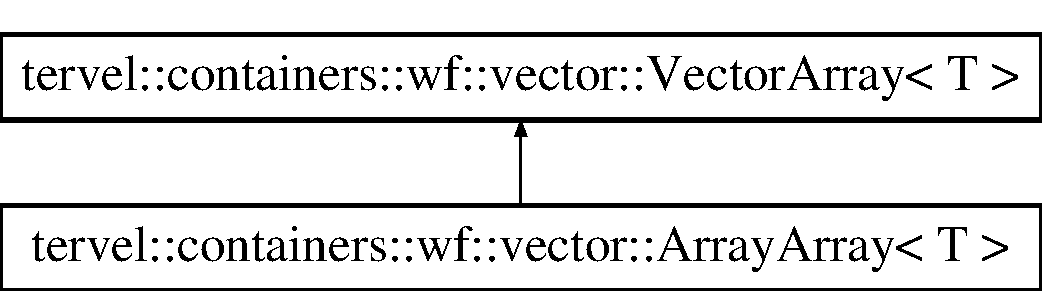
\includegraphics[height=2.000000cm]{classtervel_1_1containers_1_1wf_1_1vector_1_1_array_array}
\end{center}
\end{figure}
\subsection*{Public Member Functions}
\begin{DoxyCompactItemize}
\item 
\hyperlink{classtervel_1_1containers_1_1wf_1_1vector_1_1_array_array_a4d5831877440072dac89334eda24e6e3}{Array\+Array} (size\+\_\+t \hyperlink{classtervel_1_1containers_1_1wf_1_1vector_1_1_array_array_ae7bb842a55e3e189dc1452fb077d8459}{capacity}, T default\+\_\+value=nullptr)
\begin{DoxyCompactList}\small\item\em This class contains code related to managing elements stored in the vector It stores elements on a series of array segments, which are stored into a global vector. \end{DoxyCompactList}\item 
\hyperlink{classtervel_1_1containers_1_1wf_1_1vector_1_1_array_array_a6bac363e501d15644d71e1057db51d55}{$\sim$\+Array\+Array} ()
\item 
\hyperlink{classtervel_1_1containers_1_1wf_1_1vector_1_1_array_array_a7c46cf8d5a4df86d5d258f5e97069876}{Array\+Segment} \hyperlink{classtervel_1_1containers_1_1wf_1_1vector_1_1_array_array_a26bfbe1d092f02ca047d24856cff004c}{add\+\_\+segment} (const size\+\_\+t pos)
\begin{DoxyCompactList}\small\item\em This function adds an array segment to the arrays used to hold additional elements. \end{DoxyCompactList}\item 
\hyperlink{classtervel_1_1containers_1_1wf_1_1vector_1_1_array_array_ac3a7367d6f8ead5417cafe0026e86481}{Array\+Element} $\ast$ \hyperlink{classtervel_1_1containers_1_1wf_1_1vector_1_1_array_array_afaa4f7502ab5ae8ccbe7bb05408f600a}{get\+\_\+spot} (const size\+\_\+t raw\+\_\+pos, const bool no\+\_\+add=false)
\begin{DoxyCompactList}\small\item\em This function returns the address of the specified position. \end{DoxyCompactList}\item 
\hyperlink{classtervel_1_1containers_1_1wf_1_1vector_1_1_array_array_ac3a7367d6f8ead5417cafe0026e86481}{Array\+Element} $\ast$ \hyperlink{classtervel_1_1containers_1_1wf_1_1vector_1_1_array_array_adeae4be5c2a2f99478a8afab5d033316}{allocate\+\_\+array\+\_\+segment} (const size\+\_\+t \hyperlink{classtervel_1_1containers_1_1wf_1_1vector_1_1_array_array_ae7bb842a55e3e189dc1452fb077d8459}{capacity})
\item 
size\+\_\+t \hyperlink{classtervel_1_1containers_1_1wf_1_1vector_1_1_array_array_ae7bb842a55e3e189dc1452fb077d8459}{capacity} ()
\end{DoxyCompactItemize}
\subsection*{Private Types}
\begin{DoxyCompactItemize}
\item 
typedef std\+::atomic$<$ T $>$ \hyperlink{classtervel_1_1containers_1_1wf_1_1vector_1_1_array_array_ac3a7367d6f8ead5417cafe0026e86481}{Array\+Element}
\item 
typedef \hyperlink{classtervel_1_1containers_1_1wf_1_1vector_1_1_array_array_ac3a7367d6f8ead5417cafe0026e86481}{Array\+Element} $\ast$ \hyperlink{classtervel_1_1containers_1_1wf_1_1vector_1_1_array_array_a7c46cf8d5a4df86d5d258f5e97069876}{Array\+Segment}
\end{DoxyCompactItemize}
\subsection*{Private Attributes}
\begin{DoxyCompactItemize}
\item 
const T \hyperlink{classtervel_1_1containers_1_1wf_1_1vector_1_1_array_array_ae234686849179edcb8834753b35a181f}{default\+\_\+value\+\_\+} \{nullptr\}
\item 
std\+::atomic$<$ \hyperlink{classtervel_1_1containers_1_1wf_1_1vector_1_1_array_array_a7c46cf8d5a4df86d5d258f5e97069876}{Array\+Segment} $>$ \hyperlink{classtervel_1_1containers_1_1wf_1_1vector_1_1_array_array_a3dda9f4ccf0846e5741c03c13ae3e2b1}{array\+\_\+of\+\_\+arrays} \mbox{[}\hyperlink{classtervel_1_1containers_1_1wf_1_1vector_1_1_array_array_aee96083ae205bf8a3e2c63520320b674}{k\+\_\+max\+\_\+array\+\_\+segments\+\_\+}\mbox{]}
\item 
size\+\_\+t \hyperlink{classtervel_1_1containers_1_1wf_1_1vector_1_1_array_array_aa658a2bedb822e44a645078afbba8d1f}{offset\+\_\+}
\item 
size\+\_\+t \hyperlink{classtervel_1_1containers_1_1wf_1_1vector_1_1_array_array_a914f36d1acd29dcda33665e08af09bca}{offset\+\_\+pow\+\_\+}
\item 
std\+::atomic$<$ size\+\_\+t $>$ \hyperlink{classtervel_1_1containers_1_1wf_1_1vector_1_1_array_array_add3378d0061344bf1d6cc8f684502cc4}{current\+\_\+capacity\+\_\+}
\end{DoxyCompactItemize}
\subsection*{Static Private Attributes}
\begin{DoxyCompactItemize}
\item 
static const size\+\_\+t \hyperlink{classtervel_1_1containers_1_1wf_1_1vector_1_1_array_array_aee96083ae205bf8a3e2c63520320b674}{k\+\_\+max\+\_\+array\+\_\+segments\+\_\+} \{64\}
\end{DoxyCompactItemize}


\subsection{Member Typedef Documentation}
\hypertarget{classtervel_1_1containers_1_1wf_1_1vector_1_1_array_array_ac3a7367d6f8ead5417cafe0026e86481}{}\index{tervel\+::containers\+::wf\+::vector\+::\+Array\+Array@{tervel\+::containers\+::wf\+::vector\+::\+Array\+Array}!Array\+Element@{Array\+Element}}
\index{Array\+Element@{Array\+Element}!tervel\+::containers\+::wf\+::vector\+::\+Array\+Array@{tervel\+::containers\+::wf\+::vector\+::\+Array\+Array}}
\subsubsection[{Array\+Element}]{\setlength{\rightskip}{0pt plus 5cm}template$<$typename T $>$ typedef std\+::atomic$<$T$>$ {\bf tervel\+::containers\+::wf\+::vector\+::\+Array\+Array}$<$ T $>$\+::{\bf Array\+Element}\hspace{0.3cm}{\ttfamily [private]}}\label{classtervel_1_1containers_1_1wf_1_1vector_1_1_array_array_ac3a7367d6f8ead5417cafe0026e86481}
\hypertarget{classtervel_1_1containers_1_1wf_1_1vector_1_1_array_array_a7c46cf8d5a4df86d5d258f5e97069876}{}\index{tervel\+::containers\+::wf\+::vector\+::\+Array\+Array@{tervel\+::containers\+::wf\+::vector\+::\+Array\+Array}!Array\+Segment@{Array\+Segment}}
\index{Array\+Segment@{Array\+Segment}!tervel\+::containers\+::wf\+::vector\+::\+Array\+Array@{tervel\+::containers\+::wf\+::vector\+::\+Array\+Array}}
\subsubsection[{Array\+Segment}]{\setlength{\rightskip}{0pt plus 5cm}template$<$typename T $>$ typedef {\bf Array\+Element}$\ast$ {\bf tervel\+::containers\+::wf\+::vector\+::\+Array\+Array}$<$ T $>$\+::{\bf Array\+Segment}\hspace{0.3cm}{\ttfamily [private]}}\label{classtervel_1_1containers_1_1wf_1_1vector_1_1_array_array_a7c46cf8d5a4df86d5d258f5e97069876}


\subsection{Constructor \& Destructor Documentation}
\hypertarget{classtervel_1_1containers_1_1wf_1_1vector_1_1_array_array_a4d5831877440072dac89334eda24e6e3}{}\index{tervel\+::containers\+::wf\+::vector\+::\+Array\+Array@{tervel\+::containers\+::wf\+::vector\+::\+Array\+Array}!Array\+Array@{Array\+Array}}
\index{Array\+Array@{Array\+Array}!tervel\+::containers\+::wf\+::vector\+::\+Array\+Array@{tervel\+::containers\+::wf\+::vector\+::\+Array\+Array}}
\subsubsection[{Array\+Array(size\+\_\+t capacity, T default\+\_\+value=nullptr)}]{\setlength{\rightskip}{0pt plus 5cm}template$<$typename T $>$ {\bf tervel\+::containers\+::wf\+::vector\+::\+Array\+Array}$<$ T $>$\+::{\bf Array\+Array} (
\begin{DoxyParamCaption}
\item[{size\+\_\+t}]{capacity, }
\item[{T}]{default\+\_\+value = {\ttfamily nullptr}}
\end{DoxyParamCaption}
)\hspace{0.3cm}{\ttfamily [inline]}}\label{classtervel_1_1containers_1_1wf_1_1vector_1_1_array_array_a4d5831877440072dac89334eda24e6e3}


This class contains code related to managing elements stored in the vector It stores elements on a series of array segments, which are stored into a global vector. 

T\+O\+D\+O\+: Remove atomic type of array replace it with explicit atomic loads This will remove unnecessary memory barriers since it is a single transition type. \hypertarget{classtervel_1_1containers_1_1wf_1_1vector_1_1_array_array_a6bac363e501d15644d71e1057db51d55}{}\index{tervel\+::containers\+::wf\+::vector\+::\+Array\+Array@{tervel\+::containers\+::wf\+::vector\+::\+Array\+Array}!````~Array\+Array@{$\sim$\+Array\+Array}}
\index{````~Array\+Array@{$\sim$\+Array\+Array}!tervel\+::containers\+::wf\+::vector\+::\+Array\+Array@{tervel\+::containers\+::wf\+::vector\+::\+Array\+Array}}
\subsubsection[{$\sim$\+Array\+Array()}]{\setlength{\rightskip}{0pt plus 5cm}template$<$typename T $>$ {\bf tervel\+::containers\+::wf\+::vector\+::\+Array\+Array}$<$ T $>$\+::$\sim${\bf Array\+Array} (
\begin{DoxyParamCaption}
{}
\end{DoxyParamCaption}
)\hspace{0.3cm}{\ttfamily [inline]}}\label{classtervel_1_1containers_1_1wf_1_1vector_1_1_array_array_a6bac363e501d15644d71e1057db51d55}


\subsection{Member Function Documentation}
\hypertarget{classtervel_1_1containers_1_1wf_1_1vector_1_1_array_array_a26bfbe1d092f02ca047d24856cff004c}{}\index{tervel\+::containers\+::wf\+::vector\+::\+Array\+Array@{tervel\+::containers\+::wf\+::vector\+::\+Array\+Array}!add\+\_\+segment@{add\+\_\+segment}}
\index{add\+\_\+segment@{add\+\_\+segment}!tervel\+::containers\+::wf\+::vector\+::\+Array\+Array@{tervel\+::containers\+::wf\+::vector\+::\+Array\+Array}}
\subsubsection[{add\+\_\+segment(const size\+\_\+t pos)}]{\setlength{\rightskip}{0pt plus 5cm}template$<$typename T $>$ {\bf Array\+Segment} {\bf tervel\+::containers\+::wf\+::vector\+::\+Array\+Array}$<$ T $>$\+::add\+\_\+segment (
\begin{DoxyParamCaption}
\item[{const size\+\_\+t}]{pos}
\end{DoxyParamCaption}
)\hspace{0.3cm}{\ttfamily [inline]}}\label{classtervel_1_1containers_1_1wf_1_1vector_1_1_array_array_a26bfbe1d092f02ca047d24856cff004c}


This function adds an array segment to the arrays used to hold additional elements. 


\begin{DoxyParams}{Parameters}
{\em pos} & the slot to place the new array segment \\
\hline
\end{DoxyParams}
\begin{DoxyReturn}{Returns}
the current array segment at the specified position 
\end{DoxyReturn}
\hypertarget{classtervel_1_1containers_1_1wf_1_1vector_1_1_array_array_adeae4be5c2a2f99478a8afab5d033316}{}\index{tervel\+::containers\+::wf\+::vector\+::\+Array\+Array@{tervel\+::containers\+::wf\+::vector\+::\+Array\+Array}!allocate\+\_\+array\+\_\+segment@{allocate\+\_\+array\+\_\+segment}}
\index{allocate\+\_\+array\+\_\+segment@{allocate\+\_\+array\+\_\+segment}!tervel\+::containers\+::wf\+::vector\+::\+Array\+Array@{tervel\+::containers\+::wf\+::vector\+::\+Array\+Array}}
\subsubsection[{allocate\+\_\+array\+\_\+segment(const size\+\_\+t capacity)}]{\setlength{\rightskip}{0pt plus 5cm}template$<$typename T $>$ {\bf Array\+Element}$\ast$ {\bf tervel\+::containers\+::wf\+::vector\+::\+Array\+Array}$<$ T $>$\+::allocate\+\_\+array\+\_\+segment (
\begin{DoxyParamCaption}
\item[{const size\+\_\+t}]{capacity}
\end{DoxyParamCaption}
)\hspace{0.3cm}{\ttfamily [inline]}}\label{classtervel_1_1containers_1_1wf_1_1vector_1_1_array_array_adeae4be5c2a2f99478a8afab5d033316}
\hypertarget{classtervel_1_1containers_1_1wf_1_1vector_1_1_array_array_ae7bb842a55e3e189dc1452fb077d8459}{}\index{tervel\+::containers\+::wf\+::vector\+::\+Array\+Array@{tervel\+::containers\+::wf\+::vector\+::\+Array\+Array}!capacity@{capacity}}
\index{capacity@{capacity}!tervel\+::containers\+::wf\+::vector\+::\+Array\+Array@{tervel\+::containers\+::wf\+::vector\+::\+Array\+Array}}
\subsubsection[{capacity()}]{\setlength{\rightskip}{0pt plus 5cm}template$<$typename T $>$ size\+\_\+t {\bf tervel\+::containers\+::wf\+::vector\+::\+Array\+Array}$<$ T $>$\+::capacity (
\begin{DoxyParamCaption}
{}
\end{DoxyParamCaption}
)\hspace{0.3cm}{\ttfamily [inline]}}\label{classtervel_1_1containers_1_1wf_1_1vector_1_1_array_array_ae7bb842a55e3e189dc1452fb077d8459}
\hypertarget{classtervel_1_1containers_1_1wf_1_1vector_1_1_array_array_afaa4f7502ab5ae8ccbe7bb05408f600a}{}\index{tervel\+::containers\+::wf\+::vector\+::\+Array\+Array@{tervel\+::containers\+::wf\+::vector\+::\+Array\+Array}!get\+\_\+spot@{get\+\_\+spot}}
\index{get\+\_\+spot@{get\+\_\+spot}!tervel\+::containers\+::wf\+::vector\+::\+Array\+Array@{tervel\+::containers\+::wf\+::vector\+::\+Array\+Array}}
\subsubsection[{get\+\_\+spot(const size\+\_\+t raw\+\_\+pos, const bool no\+\_\+add=false)}]{\setlength{\rightskip}{0pt plus 5cm}template$<$typename T $>$ {\bf Array\+Element}$\ast$ {\bf tervel\+::containers\+::wf\+::vector\+::\+Array\+Array}$<$ T $>$\+::get\+\_\+spot (
\begin{DoxyParamCaption}
\item[{const size\+\_\+t}]{raw\+\_\+pos, }
\item[{const bool}]{no\+\_\+add = {\ttfamily false}}
\end{DoxyParamCaption}
)\hspace{0.3cm}{\ttfamily [inline]}, {\ttfamily [virtual]}}\label{classtervel_1_1containers_1_1wf_1_1vector_1_1_array_array_afaa4f7502ab5ae8ccbe7bb05408f600a}


This function returns the address of the specified position. 


\begin{DoxyParams}{Parameters}
{\em raw\+\_\+pos} & the position \\
\hline
{\em no\+\_\+add} & if true then it will not increase the vectors size \\
\hline
\end{DoxyParams}
\begin{DoxyReturn}{Returns}
the address of the specified positon 
\end{DoxyReturn}


Implements \hyperlink{classtervel_1_1containers_1_1wf_1_1vector_1_1_vector_array_a1ff5c1a5a86a822cfd50b48987d1857b}{tervel\+::containers\+::wf\+::vector\+::\+Vector\+Array$<$ T $>$}.



\subsection{Member Data Documentation}
\hypertarget{classtervel_1_1containers_1_1wf_1_1vector_1_1_array_array_a3dda9f4ccf0846e5741c03c13ae3e2b1}{}\index{tervel\+::containers\+::wf\+::vector\+::\+Array\+Array@{tervel\+::containers\+::wf\+::vector\+::\+Array\+Array}!array\+\_\+of\+\_\+arrays@{array\+\_\+of\+\_\+arrays}}
\index{array\+\_\+of\+\_\+arrays@{array\+\_\+of\+\_\+arrays}!tervel\+::containers\+::wf\+::vector\+::\+Array\+Array@{tervel\+::containers\+::wf\+::vector\+::\+Array\+Array}}
\subsubsection[{array\+\_\+of\+\_\+arrays}]{\setlength{\rightskip}{0pt plus 5cm}template$<$typename T $>$ std\+::atomic$<${\bf Array\+Segment}$>$ {\bf tervel\+::containers\+::wf\+::vector\+::\+Array\+Array}$<$ T $>$\+::array\+\_\+of\+\_\+arrays\mbox{[}{\bf k\+\_\+max\+\_\+array\+\_\+segments\+\_\+}\mbox{]}\hspace{0.3cm}{\ttfamily [private]}}\label{classtervel_1_1containers_1_1wf_1_1vector_1_1_array_array_a3dda9f4ccf0846e5741c03c13ae3e2b1}
\hypertarget{classtervel_1_1containers_1_1wf_1_1vector_1_1_array_array_add3378d0061344bf1d6cc8f684502cc4}{}\index{tervel\+::containers\+::wf\+::vector\+::\+Array\+Array@{tervel\+::containers\+::wf\+::vector\+::\+Array\+Array}!current\+\_\+capacity\+\_\+@{current\+\_\+capacity\+\_\+}}
\index{current\+\_\+capacity\+\_\+@{current\+\_\+capacity\+\_\+}!tervel\+::containers\+::wf\+::vector\+::\+Array\+Array@{tervel\+::containers\+::wf\+::vector\+::\+Array\+Array}}
\subsubsection[{current\+\_\+capacity\+\_\+}]{\setlength{\rightskip}{0pt plus 5cm}template$<$typename T $>$ std\+::atomic$<$size\+\_\+t$>$ {\bf tervel\+::containers\+::wf\+::vector\+::\+Array\+Array}$<$ T $>$\+::current\+\_\+capacity\+\_\+\hspace{0.3cm}{\ttfamily [private]}}\label{classtervel_1_1containers_1_1wf_1_1vector_1_1_array_array_add3378d0061344bf1d6cc8f684502cc4}
\hypertarget{classtervel_1_1containers_1_1wf_1_1vector_1_1_array_array_ae234686849179edcb8834753b35a181f}{}\index{tervel\+::containers\+::wf\+::vector\+::\+Array\+Array@{tervel\+::containers\+::wf\+::vector\+::\+Array\+Array}!default\+\_\+value\+\_\+@{default\+\_\+value\+\_\+}}
\index{default\+\_\+value\+\_\+@{default\+\_\+value\+\_\+}!tervel\+::containers\+::wf\+::vector\+::\+Array\+Array@{tervel\+::containers\+::wf\+::vector\+::\+Array\+Array}}
\subsubsection[{default\+\_\+value\+\_\+}]{\setlength{\rightskip}{0pt plus 5cm}template$<$typename T $>$ const T {\bf tervel\+::containers\+::wf\+::vector\+::\+Array\+Array}$<$ T $>$\+::default\+\_\+value\+\_\+ \{nullptr\}\hspace{0.3cm}{\ttfamily [private]}}\label{classtervel_1_1containers_1_1wf_1_1vector_1_1_array_array_ae234686849179edcb8834753b35a181f}
\hypertarget{classtervel_1_1containers_1_1wf_1_1vector_1_1_array_array_aee96083ae205bf8a3e2c63520320b674}{}\index{tervel\+::containers\+::wf\+::vector\+::\+Array\+Array@{tervel\+::containers\+::wf\+::vector\+::\+Array\+Array}!k\+\_\+max\+\_\+array\+\_\+segments\+\_\+@{k\+\_\+max\+\_\+array\+\_\+segments\+\_\+}}
\index{k\+\_\+max\+\_\+array\+\_\+segments\+\_\+@{k\+\_\+max\+\_\+array\+\_\+segments\+\_\+}!tervel\+::containers\+::wf\+::vector\+::\+Array\+Array@{tervel\+::containers\+::wf\+::vector\+::\+Array\+Array}}
\subsubsection[{k\+\_\+max\+\_\+array\+\_\+segments\+\_\+}]{\setlength{\rightskip}{0pt plus 5cm}template$<$typename T $>$ const size\+\_\+t {\bf tervel\+::containers\+::wf\+::vector\+::\+Array\+Array}$<$ T $>$\+::k\+\_\+max\+\_\+array\+\_\+segments\+\_\+ \{64\}\hspace{0.3cm}{\ttfamily [static]}, {\ttfamily [private]}}\label{classtervel_1_1containers_1_1wf_1_1vector_1_1_array_array_aee96083ae205bf8a3e2c63520320b674}
\hypertarget{classtervel_1_1containers_1_1wf_1_1vector_1_1_array_array_aa658a2bedb822e44a645078afbba8d1f}{}\index{tervel\+::containers\+::wf\+::vector\+::\+Array\+Array@{tervel\+::containers\+::wf\+::vector\+::\+Array\+Array}!offset\+\_\+@{offset\+\_\+}}
\index{offset\+\_\+@{offset\+\_\+}!tervel\+::containers\+::wf\+::vector\+::\+Array\+Array@{tervel\+::containers\+::wf\+::vector\+::\+Array\+Array}}
\subsubsection[{offset\+\_\+}]{\setlength{\rightskip}{0pt plus 5cm}template$<$typename T $>$ size\+\_\+t {\bf tervel\+::containers\+::wf\+::vector\+::\+Array\+Array}$<$ T $>$\+::offset\+\_\+\hspace{0.3cm}{\ttfamily [private]}}\label{classtervel_1_1containers_1_1wf_1_1vector_1_1_array_array_aa658a2bedb822e44a645078afbba8d1f}
\hypertarget{classtervel_1_1containers_1_1wf_1_1vector_1_1_array_array_a914f36d1acd29dcda33665e08af09bca}{}\index{tervel\+::containers\+::wf\+::vector\+::\+Array\+Array@{tervel\+::containers\+::wf\+::vector\+::\+Array\+Array}!offset\+\_\+pow\+\_\+@{offset\+\_\+pow\+\_\+}}
\index{offset\+\_\+pow\+\_\+@{offset\+\_\+pow\+\_\+}!tervel\+::containers\+::wf\+::vector\+::\+Array\+Array@{tervel\+::containers\+::wf\+::vector\+::\+Array\+Array}}
\subsubsection[{offset\+\_\+pow\+\_\+}]{\setlength{\rightskip}{0pt plus 5cm}template$<$typename T $>$ size\+\_\+t {\bf tervel\+::containers\+::wf\+::vector\+::\+Array\+Array}$<$ T $>$\+::offset\+\_\+pow\+\_\+\hspace{0.3cm}{\ttfamily [private]}}\label{classtervel_1_1containers_1_1wf_1_1vector_1_1_array_array_a914f36d1acd29dcda33665e08af09bca}


The documentation for this class was generated from the following file\+:\begin{DoxyCompactItemize}
\item 
tervel/containers/wf/vector/\hyperlink{array__array_8h}{array\+\_\+array.\+h}\end{DoxyCompactItemize}

\hypertarget{classtervel_1_1containers_1_1wf_1_1_hash_map_1_1_array_node}{}\section{tervel\+:\+:containers\+:\+:wf\+:\+:Hash\+Map$<$ Key, Value, Functor $>$\+:\+:Array\+Node Class Reference}
\label{classtervel_1_1containers_1_1wf_1_1_hash_map_1_1_array_node}\index{tervel\+::containers\+::wf\+::\+Hash\+Map$<$ Key, Value, Functor $>$\+::\+Array\+Node@{tervel\+::containers\+::wf\+::\+Hash\+Map$<$ Key, Value, Functor $>$\+::\+Array\+Node}}


This class is used to hold the secondary array structure.  


Inheritance diagram for tervel\+:\+:containers\+:\+:wf\+:\+:Hash\+Map$<$ Key, Value, Functor $>$\+:\+:Array\+Node\+:\begin{figure}[H]
\begin{center}
\leavevmode
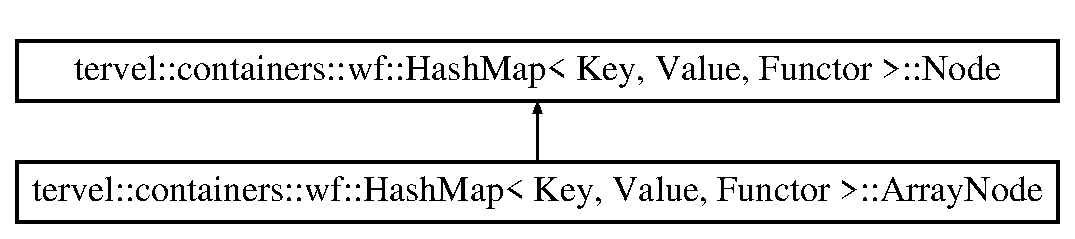
\includegraphics[height=2.000000cm]{classtervel_1_1containers_1_1wf_1_1_hash_map_1_1_array_node}
\end{center}
\end{figure}
\subsection*{Public Member Functions}
\begin{DoxyCompactItemize}
\item 
\hyperlink{classtervel_1_1containers_1_1wf_1_1_hash_map_1_1_array_node_aabfc235f98e6ec20a3f9b717161f1077}{Array\+Node} (uint64\+\_\+t len)
\item 
\hyperlink{classtervel_1_1containers_1_1wf_1_1_hash_map_1_1_array_node_af9e186fa57cd92c58acc614ccb327337}{$\sim$\+Array\+Node} ()
\begin{DoxyCompactList}\small\item\em See Notes on hash map destructor. \end{DoxyCompactList}\item 
\hyperlink{classtervel_1_1containers_1_1wf_1_1_hash_map_ab2c04cbf19034689a795208e0108fe8a}{Location} $\ast$ \hyperlink{classtervel_1_1containers_1_1wf_1_1_hash_map_1_1_array_node_a8f747038046227b9b175aa2b83f50bdf}{access} (uint64\+\_\+t pos)
\item 
bool \hyperlink{classtervel_1_1containers_1_1wf_1_1_hash_map_1_1_array_node_ad5eeaa33f2410902fbd86083e24730ca}{is\+\_\+array} ()
\item 
bool \hyperlink{classtervel_1_1containers_1_1wf_1_1_hash_map_1_1_array_node_a21681cf8d295b98084b1bebc5e434a7d}{is\+\_\+data} ()
\end{DoxyCompactItemize}
\subsection*{Private Attributes}
\begin{DoxyCompactItemize}
\item 
uint64\+\_\+t \hyperlink{classtervel_1_1containers_1_1wf_1_1_hash_map_1_1_array_node_a198987828d99d665861b727aa4a85b69}{len\+\_\+}
\item 
std\+::unique\+\_\+ptr$<$ \hyperlink{classtervel_1_1containers_1_1wf_1_1_hash_map_ab2c04cbf19034689a795208e0108fe8a}{Location}\mbox{[}$\,$\mbox{]}$>$ \hyperlink{classtervel_1_1containers_1_1wf_1_1_hash_map_1_1_array_node_a38edcefe8d4958da95ab4a464d23ae33}{internal\+\_\+array\+\_\+}
\end{DoxyCompactItemize}


\subsection{Detailed Description}
\subsubsection*{template$<$class Key, class Value, class Functor = default\+\_\+functor$<$\+Key, Value$>$$>$class tervel\+::containers\+::wf\+::\+Hash\+Map$<$ Key, Value, Functor $>$\+::\+Array\+Node}

This class is used to hold the secondary array structure. 

\subsection{Constructor \& Destructor Documentation}
\hypertarget{classtervel_1_1containers_1_1wf_1_1_hash_map_1_1_array_node_aabfc235f98e6ec20a3f9b717161f1077}{}\index{tervel\+::containers\+::wf\+::\+Hash\+Map\+::\+Array\+Node@{tervel\+::containers\+::wf\+::\+Hash\+Map\+::\+Array\+Node}!Array\+Node@{Array\+Node}}
\index{Array\+Node@{Array\+Node}!tervel\+::containers\+::wf\+::\+Hash\+Map\+::\+Array\+Node@{tervel\+::containers\+::wf\+::\+Hash\+Map\+::\+Array\+Node}}
\subsubsection[{Array\+Node(uint64\+\_\+t len)}]{\setlength{\rightskip}{0pt plus 5cm}template$<$class Key , class Value , class Functor  = default\+\_\+functor$<$\+Key, Value$>$$>$ {\bf tervel\+::containers\+::wf\+::\+Hash\+Map}$<$ Key, {\bf Value}, Functor $>$\+::Array\+Node\+::\+Array\+Node (
\begin{DoxyParamCaption}
\item[{uint64\+\_\+t}]{len}
\end{DoxyParamCaption}
)\hspace{0.3cm}{\ttfamily [inline]}, {\ttfamily [explicit]}}\label{classtervel_1_1containers_1_1wf_1_1_hash_map_1_1_array_node_aabfc235f98e6ec20a3f9b717161f1077}
\hypertarget{classtervel_1_1containers_1_1wf_1_1_hash_map_1_1_array_node_af9e186fa57cd92c58acc614ccb327337}{}\index{tervel\+::containers\+::wf\+::\+Hash\+Map\+::\+Array\+Node@{tervel\+::containers\+::wf\+::\+Hash\+Map\+::\+Array\+Node}!````~Array\+Node@{$\sim$\+Array\+Node}}
\index{````~Array\+Node@{$\sim$\+Array\+Node}!tervel\+::containers\+::wf\+::\+Hash\+Map\+::\+Array\+Node@{tervel\+::containers\+::wf\+::\+Hash\+Map\+::\+Array\+Node}}
\subsubsection[{$\sim$\+Array\+Node()}]{\setlength{\rightskip}{0pt plus 5cm}template$<$class Key , class Value , class Functor  = default\+\_\+functor$<$\+Key, Value$>$$>$ {\bf tervel\+::containers\+::wf\+::\+Hash\+Map}$<$ Key, {\bf Value}, Functor $>$\+::Array\+Node\+::$\sim$\+Array\+Node (
\begin{DoxyParamCaption}
{}
\end{DoxyParamCaption}
)\hspace{0.3cm}{\ttfamily [inline]}}\label{classtervel_1_1containers_1_1wf_1_1_hash_map_1_1_array_node_af9e186fa57cd92c58acc614ccb327337}


See Notes on hash map destructor. 



\subsection{Member Function Documentation}
\hypertarget{classtervel_1_1containers_1_1wf_1_1_hash_map_1_1_array_node_a8f747038046227b9b175aa2b83f50bdf}{}\index{tervel\+::containers\+::wf\+::\+Hash\+Map\+::\+Array\+Node@{tervel\+::containers\+::wf\+::\+Hash\+Map\+::\+Array\+Node}!access@{access}}
\index{access@{access}!tervel\+::containers\+::wf\+::\+Hash\+Map\+::\+Array\+Node@{tervel\+::containers\+::wf\+::\+Hash\+Map\+::\+Array\+Node}}
\subsubsection[{access(uint64\+\_\+t pos)}]{\setlength{\rightskip}{0pt plus 5cm}template$<$class Key , class Value , class Functor  = default\+\_\+functor$<$\+Key, Value$>$$>$ {\bf Location}$\ast$ {\bf tervel\+::containers\+::wf\+::\+Hash\+Map}$<$ Key, {\bf Value}, Functor $>$\+::Array\+Node\+::access (
\begin{DoxyParamCaption}
\item[{uint64\+\_\+t}]{pos}
\end{DoxyParamCaption}
)\hspace{0.3cm}{\ttfamily [inline]}}\label{classtervel_1_1containers_1_1wf_1_1_hash_map_1_1_array_node_a8f747038046227b9b175aa2b83f50bdf}

\begin{DoxyParams}{Parameters}
{\em pos} & The position to get the address of. \\
\hline
\end{DoxyParams}
\begin{DoxyReturn}{Returns}
the address of a position on the internal array 
\end{DoxyReturn}
\hypertarget{classtervel_1_1containers_1_1wf_1_1_hash_map_1_1_array_node_ad5eeaa33f2410902fbd86083e24730ca}{}\index{tervel\+::containers\+::wf\+::\+Hash\+Map\+::\+Array\+Node@{tervel\+::containers\+::wf\+::\+Hash\+Map\+::\+Array\+Node}!is\+\_\+array@{is\+\_\+array}}
\index{is\+\_\+array@{is\+\_\+array}!tervel\+::containers\+::wf\+::\+Hash\+Map\+::\+Array\+Node@{tervel\+::containers\+::wf\+::\+Hash\+Map\+::\+Array\+Node}}
\subsubsection[{is\+\_\+array()}]{\setlength{\rightskip}{0pt plus 5cm}template$<$class Key , class Value , class Functor  = default\+\_\+functor$<$\+Key, Value$>$$>$ bool {\bf tervel\+::containers\+::wf\+::\+Hash\+Map}$<$ Key, {\bf Value}, Functor $>$\+::Array\+Node\+::is\+\_\+array (
\begin{DoxyParamCaption}
{}
\end{DoxyParamCaption}
)\hspace{0.3cm}{\ttfamily [inline]}, {\ttfamily [virtual]}}\label{classtervel_1_1containers_1_1wf_1_1_hash_map_1_1_array_node_ad5eeaa33f2410902fbd86083e24730ca}
\begin{DoxyReturn}{Returns}
whether or not this instance is an \hyperlink{classtervel_1_1containers_1_1wf_1_1_hash_map_1_1_array_node}{Array\+Node} sub type 
\end{DoxyReturn}


Implements \hyperlink{classtervel_1_1containers_1_1wf_1_1_hash_map_1_1_node_a0908bd3151f0b1b7f8fbb6825731fd15}{tervel\+::containers\+::wf\+::\+Hash\+Map$<$ Key, Value, Functor $>$\+::\+Node}.

\hypertarget{classtervel_1_1containers_1_1wf_1_1_hash_map_1_1_array_node_a21681cf8d295b98084b1bebc5e434a7d}{}\index{tervel\+::containers\+::wf\+::\+Hash\+Map\+::\+Array\+Node@{tervel\+::containers\+::wf\+::\+Hash\+Map\+::\+Array\+Node}!is\+\_\+data@{is\+\_\+data}}
\index{is\+\_\+data@{is\+\_\+data}!tervel\+::containers\+::wf\+::\+Hash\+Map\+::\+Array\+Node@{tervel\+::containers\+::wf\+::\+Hash\+Map\+::\+Array\+Node}}
\subsubsection[{is\+\_\+data()}]{\setlength{\rightskip}{0pt plus 5cm}template$<$class Key , class Value , class Functor  = default\+\_\+functor$<$\+Key, Value$>$$>$ bool {\bf tervel\+::containers\+::wf\+::\+Hash\+Map}$<$ Key, {\bf Value}, Functor $>$\+::Array\+Node\+::is\+\_\+data (
\begin{DoxyParamCaption}
{}
\end{DoxyParamCaption}
)\hspace{0.3cm}{\ttfamily [inline]}, {\ttfamily [virtual]}}\label{classtervel_1_1containers_1_1wf_1_1_hash_map_1_1_array_node_a21681cf8d295b98084b1bebc5e434a7d}
\begin{DoxyReturn}{Returns}
whether or not this instance is an \hyperlink{classtervel_1_1containers_1_1wf_1_1_hash_map_1_1_data_node}{Data\+Node} sub type 
\end{DoxyReturn}


Implements \hyperlink{classtervel_1_1containers_1_1wf_1_1_hash_map_1_1_node_ac7cc7039cfc134def7d936f00efc2155}{tervel\+::containers\+::wf\+::\+Hash\+Map$<$ Key, Value, Functor $>$\+::\+Node}.



\subsection{Member Data Documentation}
\hypertarget{classtervel_1_1containers_1_1wf_1_1_hash_map_1_1_array_node_a38edcefe8d4958da95ab4a464d23ae33}{}\index{tervel\+::containers\+::wf\+::\+Hash\+Map\+::\+Array\+Node@{tervel\+::containers\+::wf\+::\+Hash\+Map\+::\+Array\+Node}!internal\+\_\+array\+\_\+@{internal\+\_\+array\+\_\+}}
\index{internal\+\_\+array\+\_\+@{internal\+\_\+array\+\_\+}!tervel\+::containers\+::wf\+::\+Hash\+Map\+::\+Array\+Node@{tervel\+::containers\+::wf\+::\+Hash\+Map\+::\+Array\+Node}}
\subsubsection[{internal\+\_\+array\+\_\+}]{\setlength{\rightskip}{0pt plus 5cm}template$<$class Key , class Value , class Functor  = default\+\_\+functor$<$\+Key, Value$>$$>$ std\+::unique\+\_\+ptr$<${\bf Location}\mbox{[}$\,$\mbox{]}$>$ {\bf tervel\+::containers\+::wf\+::\+Hash\+Map}$<$ Key, {\bf Value}, Functor $>$\+::Array\+Node\+::internal\+\_\+array\+\_\+\hspace{0.3cm}{\ttfamily [private]}}\label{classtervel_1_1containers_1_1wf_1_1_hash_map_1_1_array_node_a38edcefe8d4958da95ab4a464d23ae33}
\hypertarget{classtervel_1_1containers_1_1wf_1_1_hash_map_1_1_array_node_a198987828d99d665861b727aa4a85b69}{}\index{tervel\+::containers\+::wf\+::\+Hash\+Map\+::\+Array\+Node@{tervel\+::containers\+::wf\+::\+Hash\+Map\+::\+Array\+Node}!len\+\_\+@{len\+\_\+}}
\index{len\+\_\+@{len\+\_\+}!tervel\+::containers\+::wf\+::\+Hash\+Map\+::\+Array\+Node@{tervel\+::containers\+::wf\+::\+Hash\+Map\+::\+Array\+Node}}
\subsubsection[{len\+\_\+}]{\setlength{\rightskip}{0pt plus 5cm}template$<$class Key , class Value , class Functor  = default\+\_\+functor$<$\+Key, Value$>$$>$ uint64\+\_\+t {\bf tervel\+::containers\+::wf\+::\+Hash\+Map}$<$ Key, {\bf Value}, Functor $>$\+::Array\+Node\+::len\+\_\+\hspace{0.3cm}{\ttfamily [private]}}\label{classtervel_1_1containers_1_1wf_1_1_hash_map_1_1_array_node_a198987828d99d665861b727aa4a85b69}


The documentation for this class was generated from the following file\+:\begin{DoxyCompactItemize}
\item 
tervel/containers/wf/hash-\/map/\hyperlink{wf__hash__map_8h}{wf\+\_\+hash\+\_\+map.\+h}\end{DoxyCompactItemize}

\hypertarget{classtervel_1_1containers_1_1wf_1_1_hash_map_no_delete_1_1_array_node}{}\section{tervel\+:\+:containers\+:\+:wf\+:\+:Hash\+Map\+No\+Delete$<$ Key, Value, Functor $>$\+:\+:Array\+Node Class Reference}
\label{classtervel_1_1containers_1_1wf_1_1_hash_map_no_delete_1_1_array_node}\index{tervel\+::containers\+::wf\+::\+Hash\+Map\+No\+Delete$<$ Key, Value, Functor $>$\+::\+Array\+Node@{tervel\+::containers\+::wf\+::\+Hash\+Map\+No\+Delete$<$ Key, Value, Functor $>$\+::\+Array\+Node}}


This class is used to hold the secondary array structure.  


Inheritance diagram for tervel\+:\+:containers\+:\+:wf\+:\+:Hash\+Map\+No\+Delete$<$ Key, Value, Functor $>$\+:\+:Array\+Node\+:\begin{figure}[H]
\begin{center}
\leavevmode
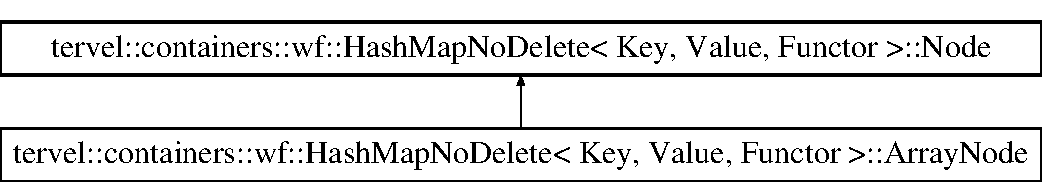
\includegraphics[height=2.000000cm]{classtervel_1_1containers_1_1wf_1_1_hash_map_no_delete_1_1_array_node}
\end{center}
\end{figure}
\subsection*{Public Member Functions}
\begin{DoxyCompactItemize}
\item 
\hyperlink{classtervel_1_1containers_1_1wf_1_1_hash_map_no_delete_1_1_array_node_ac45e67621163d45bf45f5bcc0b6f39f4}{Array\+Node} (uint64\+\_\+t len)
\item 
\hyperlink{classtervel_1_1containers_1_1wf_1_1_hash_map_no_delete_1_1_array_node_ab8e4a7e0ec552f5426083c4559a2d366}{$\sim$\+Array\+Node} ()
\begin{DoxyCompactList}\small\item\em See Notes on hash map destructor. \end{DoxyCompactList}\item 
\hyperlink{classtervel_1_1containers_1_1wf_1_1_hash_map_no_delete_af5b18c3806eb5b2d39693075d8c70ade}{Location} $\ast$ \hyperlink{classtervel_1_1containers_1_1wf_1_1_hash_map_no_delete_1_1_array_node_a405b0e610ce284c037bae98e64239599}{access} (uint64\+\_\+t pos)
\item 
bool \hyperlink{classtervel_1_1containers_1_1wf_1_1_hash_map_no_delete_1_1_array_node_a11f011931040dfd98938b073006cb04b}{is\+\_\+array} ()
\item 
bool \hyperlink{classtervel_1_1containers_1_1wf_1_1_hash_map_no_delete_1_1_array_node_a049ba7f928ab0c87be2e0466f8d29a1b}{is\+\_\+data} ()
\end{DoxyCompactItemize}
\subsection*{Private Attributes}
\begin{DoxyCompactItemize}
\item 
uint64\+\_\+t \hyperlink{classtervel_1_1containers_1_1wf_1_1_hash_map_no_delete_1_1_array_node_a5f281eee813a9ccf8357399782bde1a3}{len\+\_\+}
\item 
std\+::unique\+\_\+ptr$<$ \hyperlink{classtervel_1_1containers_1_1wf_1_1_hash_map_no_delete_af5b18c3806eb5b2d39693075d8c70ade}{Location}\mbox{[}$\,$\mbox{]}$>$ \hyperlink{classtervel_1_1containers_1_1wf_1_1_hash_map_no_delete_1_1_array_node_a7856c599048010921c610f1b6c5ef6e7}{internal\+\_\+array\+\_\+}
\end{DoxyCompactItemize}


\subsection{Detailed Description}
\subsubsection*{template$<$class Key, class Value, class Functor = default\+\_\+functor$<$\+Key, Value$>$$>$class tervel\+::containers\+::wf\+::\+Hash\+Map\+No\+Delete$<$ Key, Value, Functor $>$\+::\+Array\+Node}

This class is used to hold the secondary array structure. 

\subsection{Constructor \& Destructor Documentation}
\hypertarget{classtervel_1_1containers_1_1wf_1_1_hash_map_no_delete_1_1_array_node_ac45e67621163d45bf45f5bcc0b6f39f4}{}\index{tervel\+::containers\+::wf\+::\+Hash\+Map\+No\+Delete\+::\+Array\+Node@{tervel\+::containers\+::wf\+::\+Hash\+Map\+No\+Delete\+::\+Array\+Node}!Array\+Node@{Array\+Node}}
\index{Array\+Node@{Array\+Node}!tervel\+::containers\+::wf\+::\+Hash\+Map\+No\+Delete\+::\+Array\+Node@{tervel\+::containers\+::wf\+::\+Hash\+Map\+No\+Delete\+::\+Array\+Node}}
\subsubsection[{Array\+Node(uint64\+\_\+t len)}]{\setlength{\rightskip}{0pt plus 5cm}template$<$class Key , class Value , class Functor  = default\+\_\+functor$<$\+Key, Value$>$$>$ {\bf tervel\+::containers\+::wf\+::\+Hash\+Map\+No\+Delete}$<$ Key, {\bf Value}, Functor $>$\+::Array\+Node\+::\+Array\+Node (
\begin{DoxyParamCaption}
\item[{uint64\+\_\+t}]{len}
\end{DoxyParamCaption}
)\hspace{0.3cm}{\ttfamily [inline]}, {\ttfamily [explicit]}}\label{classtervel_1_1containers_1_1wf_1_1_hash_map_no_delete_1_1_array_node_ac45e67621163d45bf45f5bcc0b6f39f4}
\hypertarget{classtervel_1_1containers_1_1wf_1_1_hash_map_no_delete_1_1_array_node_ab8e4a7e0ec552f5426083c4559a2d366}{}\index{tervel\+::containers\+::wf\+::\+Hash\+Map\+No\+Delete\+::\+Array\+Node@{tervel\+::containers\+::wf\+::\+Hash\+Map\+No\+Delete\+::\+Array\+Node}!````~Array\+Node@{$\sim$\+Array\+Node}}
\index{````~Array\+Node@{$\sim$\+Array\+Node}!tervel\+::containers\+::wf\+::\+Hash\+Map\+No\+Delete\+::\+Array\+Node@{tervel\+::containers\+::wf\+::\+Hash\+Map\+No\+Delete\+::\+Array\+Node}}
\subsubsection[{$\sim$\+Array\+Node()}]{\setlength{\rightskip}{0pt plus 5cm}template$<$class Key , class Value , class Functor  = default\+\_\+functor$<$\+Key, Value$>$$>$ {\bf tervel\+::containers\+::wf\+::\+Hash\+Map\+No\+Delete}$<$ Key, {\bf Value}, Functor $>$\+::Array\+Node\+::$\sim$\+Array\+Node (
\begin{DoxyParamCaption}
{}
\end{DoxyParamCaption}
)\hspace{0.3cm}{\ttfamily [inline]}}\label{classtervel_1_1containers_1_1wf_1_1_hash_map_no_delete_1_1_array_node_ab8e4a7e0ec552f5426083c4559a2d366}


See Notes on hash map destructor. 



\subsection{Member Function Documentation}
\hypertarget{classtervel_1_1containers_1_1wf_1_1_hash_map_no_delete_1_1_array_node_a405b0e610ce284c037bae98e64239599}{}\index{tervel\+::containers\+::wf\+::\+Hash\+Map\+No\+Delete\+::\+Array\+Node@{tervel\+::containers\+::wf\+::\+Hash\+Map\+No\+Delete\+::\+Array\+Node}!access@{access}}
\index{access@{access}!tervel\+::containers\+::wf\+::\+Hash\+Map\+No\+Delete\+::\+Array\+Node@{tervel\+::containers\+::wf\+::\+Hash\+Map\+No\+Delete\+::\+Array\+Node}}
\subsubsection[{access(uint64\+\_\+t pos)}]{\setlength{\rightskip}{0pt plus 5cm}template$<$class Key , class Value , class Functor  = default\+\_\+functor$<$\+Key, Value$>$$>$ {\bf Location}$\ast$ {\bf tervel\+::containers\+::wf\+::\+Hash\+Map\+No\+Delete}$<$ Key, {\bf Value}, Functor $>$\+::Array\+Node\+::access (
\begin{DoxyParamCaption}
\item[{uint64\+\_\+t}]{pos}
\end{DoxyParamCaption}
)\hspace{0.3cm}{\ttfamily [inline]}}\label{classtervel_1_1containers_1_1wf_1_1_hash_map_no_delete_1_1_array_node_a405b0e610ce284c037bae98e64239599}

\begin{DoxyParams}{Parameters}
{\em pos} & The position to get the address of. \\
\hline
\end{DoxyParams}
\begin{DoxyReturn}{Returns}
the address of a position on the internal array 
\end{DoxyReturn}
\hypertarget{classtervel_1_1containers_1_1wf_1_1_hash_map_no_delete_1_1_array_node_a11f011931040dfd98938b073006cb04b}{}\index{tervel\+::containers\+::wf\+::\+Hash\+Map\+No\+Delete\+::\+Array\+Node@{tervel\+::containers\+::wf\+::\+Hash\+Map\+No\+Delete\+::\+Array\+Node}!is\+\_\+array@{is\+\_\+array}}
\index{is\+\_\+array@{is\+\_\+array}!tervel\+::containers\+::wf\+::\+Hash\+Map\+No\+Delete\+::\+Array\+Node@{tervel\+::containers\+::wf\+::\+Hash\+Map\+No\+Delete\+::\+Array\+Node}}
\subsubsection[{is\+\_\+array()}]{\setlength{\rightskip}{0pt plus 5cm}template$<$class Key , class Value , class Functor  = default\+\_\+functor$<$\+Key, Value$>$$>$ bool {\bf tervel\+::containers\+::wf\+::\+Hash\+Map\+No\+Delete}$<$ Key, {\bf Value}, Functor $>$\+::Array\+Node\+::is\+\_\+array (
\begin{DoxyParamCaption}
{}
\end{DoxyParamCaption}
)\hspace{0.3cm}{\ttfamily [inline]}, {\ttfamily [virtual]}}\label{classtervel_1_1containers_1_1wf_1_1_hash_map_no_delete_1_1_array_node_a11f011931040dfd98938b073006cb04b}
\begin{DoxyReturn}{Returns}
whether or not this instance is an \hyperlink{classtervel_1_1containers_1_1wf_1_1_hash_map_no_delete_1_1_array_node}{Array\+Node} sub type 
\end{DoxyReturn}


Implements \hyperlink{classtervel_1_1containers_1_1wf_1_1_hash_map_no_delete_1_1_node_a551c6b4900b06efe3fc1d4de7c25963b}{tervel\+::containers\+::wf\+::\+Hash\+Map\+No\+Delete$<$ Key, Value, Functor $>$\+::\+Node}.

\hypertarget{classtervel_1_1containers_1_1wf_1_1_hash_map_no_delete_1_1_array_node_a049ba7f928ab0c87be2e0466f8d29a1b}{}\index{tervel\+::containers\+::wf\+::\+Hash\+Map\+No\+Delete\+::\+Array\+Node@{tervel\+::containers\+::wf\+::\+Hash\+Map\+No\+Delete\+::\+Array\+Node}!is\+\_\+data@{is\+\_\+data}}
\index{is\+\_\+data@{is\+\_\+data}!tervel\+::containers\+::wf\+::\+Hash\+Map\+No\+Delete\+::\+Array\+Node@{tervel\+::containers\+::wf\+::\+Hash\+Map\+No\+Delete\+::\+Array\+Node}}
\subsubsection[{is\+\_\+data()}]{\setlength{\rightskip}{0pt plus 5cm}template$<$class Key , class Value , class Functor  = default\+\_\+functor$<$\+Key, Value$>$$>$ bool {\bf tervel\+::containers\+::wf\+::\+Hash\+Map\+No\+Delete}$<$ Key, {\bf Value}, Functor $>$\+::Array\+Node\+::is\+\_\+data (
\begin{DoxyParamCaption}
{}
\end{DoxyParamCaption}
)\hspace{0.3cm}{\ttfamily [inline]}, {\ttfamily [virtual]}}\label{classtervel_1_1containers_1_1wf_1_1_hash_map_no_delete_1_1_array_node_a049ba7f928ab0c87be2e0466f8d29a1b}
\begin{DoxyReturn}{Returns}
whether or not this instance is an \hyperlink{classtervel_1_1containers_1_1wf_1_1_hash_map_no_delete_1_1_data_node}{Data\+Node} sub type 
\end{DoxyReturn}


Implements \hyperlink{classtervel_1_1containers_1_1wf_1_1_hash_map_no_delete_1_1_node_a03ef6395f93104d0313296773be36b3c}{tervel\+::containers\+::wf\+::\+Hash\+Map\+No\+Delete$<$ Key, Value, Functor $>$\+::\+Node}.



\subsection{Member Data Documentation}
\hypertarget{classtervel_1_1containers_1_1wf_1_1_hash_map_no_delete_1_1_array_node_a7856c599048010921c610f1b6c5ef6e7}{}\index{tervel\+::containers\+::wf\+::\+Hash\+Map\+No\+Delete\+::\+Array\+Node@{tervel\+::containers\+::wf\+::\+Hash\+Map\+No\+Delete\+::\+Array\+Node}!internal\+\_\+array\+\_\+@{internal\+\_\+array\+\_\+}}
\index{internal\+\_\+array\+\_\+@{internal\+\_\+array\+\_\+}!tervel\+::containers\+::wf\+::\+Hash\+Map\+No\+Delete\+::\+Array\+Node@{tervel\+::containers\+::wf\+::\+Hash\+Map\+No\+Delete\+::\+Array\+Node}}
\subsubsection[{internal\+\_\+array\+\_\+}]{\setlength{\rightskip}{0pt plus 5cm}template$<$class Key , class Value , class Functor  = default\+\_\+functor$<$\+Key, Value$>$$>$ std\+::unique\+\_\+ptr$<${\bf Location}\mbox{[}$\,$\mbox{]}$>$ {\bf tervel\+::containers\+::wf\+::\+Hash\+Map\+No\+Delete}$<$ Key, {\bf Value}, Functor $>$\+::Array\+Node\+::internal\+\_\+array\+\_\+\hspace{0.3cm}{\ttfamily [private]}}\label{classtervel_1_1containers_1_1wf_1_1_hash_map_no_delete_1_1_array_node_a7856c599048010921c610f1b6c5ef6e7}
\hypertarget{classtervel_1_1containers_1_1wf_1_1_hash_map_no_delete_1_1_array_node_a5f281eee813a9ccf8357399782bde1a3}{}\index{tervel\+::containers\+::wf\+::\+Hash\+Map\+No\+Delete\+::\+Array\+Node@{tervel\+::containers\+::wf\+::\+Hash\+Map\+No\+Delete\+::\+Array\+Node}!len\+\_\+@{len\+\_\+}}
\index{len\+\_\+@{len\+\_\+}!tervel\+::containers\+::wf\+::\+Hash\+Map\+No\+Delete\+::\+Array\+Node@{tervel\+::containers\+::wf\+::\+Hash\+Map\+No\+Delete\+::\+Array\+Node}}
\subsubsection[{len\+\_\+}]{\setlength{\rightskip}{0pt plus 5cm}template$<$class Key , class Value , class Functor  = default\+\_\+functor$<$\+Key, Value$>$$>$ uint64\+\_\+t {\bf tervel\+::containers\+::wf\+::\+Hash\+Map\+No\+Delete}$<$ Key, {\bf Value}, Functor $>$\+::Array\+Node\+::len\+\_\+\hspace{0.3cm}{\ttfamily [private]}}\label{classtervel_1_1containers_1_1wf_1_1_hash_map_no_delete_1_1_array_node_a5f281eee813a9ccf8357399782bde1a3}


The documentation for this class was generated from the following file\+:\begin{DoxyCompactItemize}
\item 
tervel/containers/wf/hash-\/map/\hyperlink{wf__hash__map__no__delete_8h}{wf\+\_\+hash\+\_\+map\+\_\+no\+\_\+delete.\+h}\end{DoxyCompactItemize}

\hypertarget{classtervel_1_1containers_1_1wf_1_1_ring_buffer_1_1_buffer_op}{}\section{tervel\+:\+:containers\+:\+:wf\+:\+:Ring\+Buffer$<$ T $>$\+:\+:Buffer\+Op Class Reference}
\label{classtervel_1_1containers_1_1wf_1_1_ring_buffer_1_1_buffer_op}\index{tervel\+::containers\+::wf\+::\+Ring\+Buffer$<$ T $>$\+::\+Buffer\+Op@{tervel\+::containers\+::wf\+::\+Ring\+Buffer$<$ T $>$\+::\+Buffer\+Op}}


{\ttfamily \#include $<$ring\+\_\+buffer\+\_\+op.\+h$>$}

Inheritance diagram for tervel\+:\+:containers\+:\+:wf\+:\+:Ring\+Buffer$<$ T $>$\+:\+:Buffer\+Op\+:\begin{figure}[H]
\begin{center}
\leavevmode
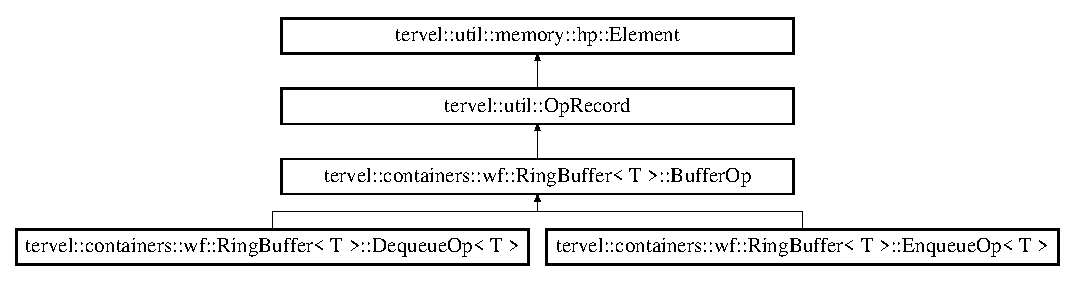
\includegraphics[height=3.323442cm]{classtervel_1_1containers_1_1wf_1_1_ring_buffer_1_1_buffer_op}
\end{center}
\end{figure}
\subsection*{Public Member Functions}
\begin{DoxyCompactItemize}
\item 
\hyperlink{classtervel_1_1containers_1_1wf_1_1_ring_buffer_1_1_buffer_op_a3beeae0f911b913a997c4841392c577c}{Buffer\+Op} (\hyperlink{classtervel_1_1containers_1_1wf_1_1_ring_buffer}{Ring\+Buffer}$<$ T $>$ $\ast$rb)
\item 
\hyperlink{classtervel_1_1containers_1_1wf_1_1_ring_buffer_1_1_buffer_op_aed38cc45945b5fe9fa6020554ebe8543}{$\sim$\+Buffer\+Op} ()
\item 
virtual void $\ast$ \hyperlink{classtervel_1_1containers_1_1wf_1_1_ring_buffer_1_1_buffer_op_a345d7432fa98f44f1620f5f718ff7a1e}{associate} (\hyperlink{classtervel_1_1containers_1_1wf_1_1_ring_buffer_1_1_helper}{Helper} $\ast$h)=0
\item 
bool \hyperlink{classtervel_1_1containers_1_1wf_1_1_ring_buffer_1_1_buffer_op_a118e970ddcaef2f6e932244fc88d99e8}{priv\+Associate} (\hyperlink{classtervel_1_1containers_1_1wf_1_1_ring_buffer_1_1_helper}{Helper} $\ast$h)
\item 
bool \hyperlink{classtervel_1_1containers_1_1wf_1_1_ring_buffer_1_1_buffer_op_adb1f2fd8c3d16d7024c00d49124da0b5}{valid} (\hyperlink{classtervel_1_1containers_1_1wf_1_1_ring_buffer_1_1_helper}{Helper} $\ast$h)
\item 
void \hyperlink{classtervel_1_1containers_1_1wf_1_1_ring_buffer_1_1_buffer_op_a1afc3cef307a996571b654f41650dc4e}{fail} ()
\item 
bool \hyperlink{classtervel_1_1containers_1_1wf_1_1_ring_buffer_1_1_buffer_op_a90977eb87ba55abaabe0edb32ab609e7}{is\+Fail} (\hyperlink{classtervel_1_1containers_1_1wf_1_1_ring_buffer_1_1_helper}{Helper} $\ast$\&h)
\item 
\hyperlink{classtervel_1_1containers_1_1wf_1_1_ring_buffer_1_1_helper}{Helper} $\ast$ \hyperlink{classtervel_1_1containers_1_1wf_1_1_ring_buffer_1_1_buffer_op_ab67453c6a60a8cd47aefc9a5bece510a}{get\+Helper} ()
\item 
bool \hyperlink{classtervel_1_1containers_1_1wf_1_1_ring_buffer_1_1_buffer_op_a7b64b9df1ce447b38bbf6d874edea54d}{not\+Done} ()
\item 
\hyperlink{classtervel_1_1containers_1_1wf_1_1_ring_buffer_1_1_buffer_op_ac6f6c55dff8bae48cccce1357848d32f}{D\+I\+S\+A\+L\+L\+O\+W\+\_\+\+C\+O\+P\+Y\+\_\+\+A\+N\+D\+\_\+\+A\+S\+S\+I\+G\+N} (\hyperlink{classtervel_1_1containers_1_1wf_1_1_ring_buffer_1_1_buffer_op}{Buffer\+Op})
\end{DoxyCompactItemize}
\subsection*{Public Attributes}
\begin{DoxyCompactItemize}
\item 
\hyperlink{classtervel_1_1containers_1_1wf_1_1_ring_buffer}{Ring\+Buffer}$<$ T $>$ $\ast$ \hyperlink{classtervel_1_1containers_1_1wf_1_1_ring_buffer_1_1_buffer_op_a2f8fe07f0f1b404a6cecb43564795973}{rb\+\_\+}
\item 
std\+::atomic$<$ \hyperlink{classtervel_1_1containers_1_1wf_1_1_ring_buffer_1_1_helper}{Helper} $\ast$ $>$ \hyperlink{classtervel_1_1containers_1_1wf_1_1_ring_buffer_1_1_buffer_op_a27d2feab0bcff8ba7f23ffed677b7a6e}{helper\+\_\+} \{nullptr\}
\end{DoxyCompactItemize}
\subsection*{Static Public Attributes}
\begin{DoxyCompactItemize}
\item 
static constexpr \hyperlink{classtervel_1_1containers_1_1wf_1_1_ring_buffer_1_1_helper}{Helper} $\ast$ \hyperlink{classtervel_1_1containers_1_1wf_1_1_ring_buffer_1_1_buffer_op_abdce2129a65d213a747850f8dbe0c6b8}{fail\+\_\+val\+\_\+} = reinterpret\+\_\+cast$<$\hyperlink{classtervel_1_1containers_1_1wf_1_1_ring_buffer_1_1_helper}{Helper} $\ast$$>$(0x1\+L)
\end{DoxyCompactItemize}


\subsection{Constructor \& Destructor Documentation}
\hypertarget{classtervel_1_1containers_1_1wf_1_1_ring_buffer_1_1_buffer_op_a3beeae0f911b913a997c4841392c577c}{}\index{tervel\+::containers\+::wf\+::\+Ring\+Buffer\+::\+Buffer\+Op@{tervel\+::containers\+::wf\+::\+Ring\+Buffer\+::\+Buffer\+Op}!Buffer\+Op@{Buffer\+Op}}
\index{Buffer\+Op@{Buffer\+Op}!tervel\+::containers\+::wf\+::\+Ring\+Buffer\+::\+Buffer\+Op@{tervel\+::containers\+::wf\+::\+Ring\+Buffer\+::\+Buffer\+Op}}
\subsubsection[{Buffer\+Op(\+Ring\+Buffer$<$ T $>$ $\ast$rb)}]{\setlength{\rightskip}{0pt plus 5cm}template$<$typename T$>$ {\bf tervel\+::containers\+::wf\+::\+Ring\+Buffer}$<$ T $>$\+::Buffer\+Op\+::\+Buffer\+Op (
\begin{DoxyParamCaption}
\item[{{\bf Ring\+Buffer}$<$ T $>$ $\ast$}]{rb}
\end{DoxyParamCaption}
)\hspace{0.3cm}{\ttfamily [inline]}}\label{classtervel_1_1containers_1_1wf_1_1_ring_buffer_1_1_buffer_op_a3beeae0f911b913a997c4841392c577c}
\hypertarget{classtervel_1_1containers_1_1wf_1_1_ring_buffer_1_1_buffer_op_aed38cc45945b5fe9fa6020554ebe8543}{}\index{tervel\+::containers\+::wf\+::\+Ring\+Buffer\+::\+Buffer\+Op@{tervel\+::containers\+::wf\+::\+Ring\+Buffer\+::\+Buffer\+Op}!````~Buffer\+Op@{$\sim$\+Buffer\+Op}}
\index{````~Buffer\+Op@{$\sim$\+Buffer\+Op}!tervel\+::containers\+::wf\+::\+Ring\+Buffer\+::\+Buffer\+Op@{tervel\+::containers\+::wf\+::\+Ring\+Buffer\+::\+Buffer\+Op}}
\subsubsection[{$\sim$\+Buffer\+Op()}]{\setlength{\rightskip}{0pt plus 5cm}template$<$typename T$>$ {\bf tervel\+::containers\+::wf\+::\+Ring\+Buffer}$<$ T $>$\+::Buffer\+Op\+::$\sim$\+Buffer\+Op (
\begin{DoxyParamCaption}
{}
\end{DoxyParamCaption}
)\hspace{0.3cm}{\ttfamily [inline]}}\label{classtervel_1_1containers_1_1wf_1_1_ring_buffer_1_1_buffer_op_aed38cc45945b5fe9fa6020554ebe8543}


\subsection{Member Function Documentation}
\hypertarget{classtervel_1_1containers_1_1wf_1_1_ring_buffer_1_1_buffer_op_a345d7432fa98f44f1620f5f718ff7a1e}{}\index{tervel\+::containers\+::wf\+::\+Ring\+Buffer\+::\+Buffer\+Op@{tervel\+::containers\+::wf\+::\+Ring\+Buffer\+::\+Buffer\+Op}!associate@{associate}}
\index{associate@{associate}!tervel\+::containers\+::wf\+::\+Ring\+Buffer\+::\+Buffer\+Op@{tervel\+::containers\+::wf\+::\+Ring\+Buffer\+::\+Buffer\+Op}}
\subsubsection[{associate(\+Helper $\ast$h)=0}]{\setlength{\rightskip}{0pt plus 5cm}template$<$typename T$>$ virtual void$\ast$ {\bf tervel\+::containers\+::wf\+::\+Ring\+Buffer}$<$ T $>$\+::Buffer\+Op\+::associate (
\begin{DoxyParamCaption}
\item[{{\bf Helper} $\ast$}]{h}
\end{DoxyParamCaption}
)\hspace{0.3cm}{\ttfamily [pure virtual]}}\label{classtervel_1_1containers_1_1wf_1_1_ring_buffer_1_1_buffer_op_a345d7432fa98f44f1620f5f718ff7a1e}


Implemented in \hyperlink{classtervel_1_1containers_1_1wf_1_1_ring_buffer_1_1_enqueue_op_a746cece514a2d8189bad01c04a1cf00c}{tervel\+::containers\+::wf\+::\+Ring\+Buffer$<$ T $>$\+::\+Enqueue\+Op$<$ T $>$}, and \hyperlink{classtervel_1_1containers_1_1wf_1_1_ring_buffer_1_1_dequeue_op_a9c2398124db300ce3b28e3541e48d347}{tervel\+::containers\+::wf\+::\+Ring\+Buffer$<$ T $>$\+::\+Dequeue\+Op$<$ T $>$}.

\hypertarget{classtervel_1_1containers_1_1wf_1_1_ring_buffer_1_1_buffer_op_ac6f6c55dff8bae48cccce1357848d32f}{}\index{tervel\+::containers\+::wf\+::\+Ring\+Buffer\+::\+Buffer\+Op@{tervel\+::containers\+::wf\+::\+Ring\+Buffer\+::\+Buffer\+Op}!D\+I\+S\+A\+L\+L\+O\+W\+\_\+\+C\+O\+P\+Y\+\_\+\+A\+N\+D\+\_\+\+A\+S\+S\+I\+G\+N@{D\+I\+S\+A\+L\+L\+O\+W\+\_\+\+C\+O\+P\+Y\+\_\+\+A\+N\+D\+\_\+\+A\+S\+S\+I\+G\+N}}
\index{D\+I\+S\+A\+L\+L\+O\+W\+\_\+\+C\+O\+P\+Y\+\_\+\+A\+N\+D\+\_\+\+A\+S\+S\+I\+G\+N@{D\+I\+S\+A\+L\+L\+O\+W\+\_\+\+C\+O\+P\+Y\+\_\+\+A\+N\+D\+\_\+\+A\+S\+S\+I\+G\+N}!tervel\+::containers\+::wf\+::\+Ring\+Buffer\+::\+Buffer\+Op@{tervel\+::containers\+::wf\+::\+Ring\+Buffer\+::\+Buffer\+Op}}
\subsubsection[{D\+I\+S\+A\+L\+L\+O\+W\+\_\+\+C\+O\+P\+Y\+\_\+\+A\+N\+D\+\_\+\+A\+S\+S\+I\+G\+N(\+Buffer\+Op)}]{\setlength{\rightskip}{0pt plus 5cm}template$<$typename T$>$ {\bf tervel\+::containers\+::wf\+::\+Ring\+Buffer}$<$ T $>$\+::Buffer\+Op\+::\+D\+I\+S\+A\+L\+L\+O\+W\+\_\+\+C\+O\+P\+Y\+\_\+\+A\+N\+D\+\_\+\+A\+S\+S\+I\+G\+N (
\begin{DoxyParamCaption}
\item[{{\bf Buffer\+Op}}]{}
\end{DoxyParamCaption}
)}\label{classtervel_1_1containers_1_1wf_1_1_ring_buffer_1_1_buffer_op_ac6f6c55dff8bae48cccce1357848d32f}
\hypertarget{classtervel_1_1containers_1_1wf_1_1_ring_buffer_1_1_buffer_op_a1afc3cef307a996571b654f41650dc4e}{}\index{tervel\+::containers\+::wf\+::\+Ring\+Buffer\+::\+Buffer\+Op@{tervel\+::containers\+::wf\+::\+Ring\+Buffer\+::\+Buffer\+Op}!fail@{fail}}
\index{fail@{fail}!tervel\+::containers\+::wf\+::\+Ring\+Buffer\+::\+Buffer\+Op@{tervel\+::containers\+::wf\+::\+Ring\+Buffer\+::\+Buffer\+Op}}
\subsubsection[{fail()}]{\setlength{\rightskip}{0pt plus 5cm}template$<$typename T$>$ void {\bf tervel\+::containers\+::wf\+::\+Ring\+Buffer}$<$ T $>$\+::Buffer\+Op\+::fail (
\begin{DoxyParamCaption}
{}
\end{DoxyParamCaption}
)\hspace{0.3cm}{\ttfamily [inline]}}\label{classtervel_1_1containers_1_1wf_1_1_ring_buffer_1_1_buffer_op_a1afc3cef307a996571b654f41650dc4e}
\hypertarget{classtervel_1_1containers_1_1wf_1_1_ring_buffer_1_1_buffer_op_ab67453c6a60a8cd47aefc9a5bece510a}{}\index{tervel\+::containers\+::wf\+::\+Ring\+Buffer\+::\+Buffer\+Op@{tervel\+::containers\+::wf\+::\+Ring\+Buffer\+::\+Buffer\+Op}!get\+Helper@{get\+Helper}}
\index{get\+Helper@{get\+Helper}!tervel\+::containers\+::wf\+::\+Ring\+Buffer\+::\+Buffer\+Op@{tervel\+::containers\+::wf\+::\+Ring\+Buffer\+::\+Buffer\+Op}}
\subsubsection[{get\+Helper()}]{\setlength{\rightskip}{0pt plus 5cm}template$<$typename T$>$ {\bf Helper}$\ast$ {\bf tervel\+::containers\+::wf\+::\+Ring\+Buffer}$<$ T $>$\+::Buffer\+Op\+::get\+Helper (
\begin{DoxyParamCaption}
{}
\end{DoxyParamCaption}
)\hspace{0.3cm}{\ttfamily [inline]}}\label{classtervel_1_1containers_1_1wf_1_1_ring_buffer_1_1_buffer_op_ab67453c6a60a8cd47aefc9a5bece510a}
\hypertarget{classtervel_1_1containers_1_1wf_1_1_ring_buffer_1_1_buffer_op_a90977eb87ba55abaabe0edb32ab609e7}{}\index{tervel\+::containers\+::wf\+::\+Ring\+Buffer\+::\+Buffer\+Op@{tervel\+::containers\+::wf\+::\+Ring\+Buffer\+::\+Buffer\+Op}!is\+Fail@{is\+Fail}}
\index{is\+Fail@{is\+Fail}!tervel\+::containers\+::wf\+::\+Ring\+Buffer\+::\+Buffer\+Op@{tervel\+::containers\+::wf\+::\+Ring\+Buffer\+::\+Buffer\+Op}}
\subsubsection[{is\+Fail(\+Helper $\ast$\&h)}]{\setlength{\rightskip}{0pt plus 5cm}template$<$typename T$>$ bool {\bf tervel\+::containers\+::wf\+::\+Ring\+Buffer}$<$ T $>$\+::Buffer\+Op\+::is\+Fail (
\begin{DoxyParamCaption}
\item[{{\bf Helper} $\ast$\&}]{h}
\end{DoxyParamCaption}
)\hspace{0.3cm}{\ttfamily [inline]}}\label{classtervel_1_1containers_1_1wf_1_1_ring_buffer_1_1_buffer_op_a90977eb87ba55abaabe0edb32ab609e7}
\hypertarget{classtervel_1_1containers_1_1wf_1_1_ring_buffer_1_1_buffer_op_a7b64b9df1ce447b38bbf6d874edea54d}{}\index{tervel\+::containers\+::wf\+::\+Ring\+Buffer\+::\+Buffer\+Op@{tervel\+::containers\+::wf\+::\+Ring\+Buffer\+::\+Buffer\+Op}!not\+Done@{not\+Done}}
\index{not\+Done@{not\+Done}!tervel\+::containers\+::wf\+::\+Ring\+Buffer\+::\+Buffer\+Op@{tervel\+::containers\+::wf\+::\+Ring\+Buffer\+::\+Buffer\+Op}}
\subsubsection[{not\+Done()}]{\setlength{\rightskip}{0pt plus 5cm}template$<$typename T$>$ bool {\bf tervel\+::containers\+::wf\+::\+Ring\+Buffer}$<$ T $>$\+::Buffer\+Op\+::not\+Done (
\begin{DoxyParamCaption}
{}
\end{DoxyParamCaption}
)\hspace{0.3cm}{\ttfamily [inline]}}\label{classtervel_1_1containers_1_1wf_1_1_ring_buffer_1_1_buffer_op_a7b64b9df1ce447b38bbf6d874edea54d}
\hypertarget{classtervel_1_1containers_1_1wf_1_1_ring_buffer_1_1_buffer_op_a118e970ddcaef2f6e932244fc88d99e8}{}\index{tervel\+::containers\+::wf\+::\+Ring\+Buffer\+::\+Buffer\+Op@{tervel\+::containers\+::wf\+::\+Ring\+Buffer\+::\+Buffer\+Op}!priv\+Associate@{priv\+Associate}}
\index{priv\+Associate@{priv\+Associate}!tervel\+::containers\+::wf\+::\+Ring\+Buffer\+::\+Buffer\+Op@{tervel\+::containers\+::wf\+::\+Ring\+Buffer\+::\+Buffer\+Op}}
\subsubsection[{priv\+Associate(\+Helper $\ast$h)}]{\setlength{\rightskip}{0pt plus 5cm}template$<$typename T$>$ bool {\bf tervel\+::containers\+::wf\+::\+Ring\+Buffer}$<$ T $>$\+::Buffer\+Op\+::priv\+Associate (
\begin{DoxyParamCaption}
\item[{{\bf Helper} $\ast$}]{h}
\end{DoxyParamCaption}
)\hspace{0.3cm}{\ttfamily [inline]}}\label{classtervel_1_1containers_1_1wf_1_1_ring_buffer_1_1_buffer_op_a118e970ddcaef2f6e932244fc88d99e8}
\hypertarget{classtervel_1_1containers_1_1wf_1_1_ring_buffer_1_1_buffer_op_adb1f2fd8c3d16d7024c00d49124da0b5}{}\index{tervel\+::containers\+::wf\+::\+Ring\+Buffer\+::\+Buffer\+Op@{tervel\+::containers\+::wf\+::\+Ring\+Buffer\+::\+Buffer\+Op}!valid@{valid}}
\index{valid@{valid}!tervel\+::containers\+::wf\+::\+Ring\+Buffer\+::\+Buffer\+Op@{tervel\+::containers\+::wf\+::\+Ring\+Buffer\+::\+Buffer\+Op}}
\subsubsection[{valid(\+Helper $\ast$h)}]{\setlength{\rightskip}{0pt plus 5cm}template$<$typename T$>$ bool {\bf tervel\+::containers\+::wf\+::\+Ring\+Buffer}$<$ T $>$\+::Buffer\+Op\+::valid (
\begin{DoxyParamCaption}
\item[{{\bf Helper} $\ast$}]{h}
\end{DoxyParamCaption}
)\hspace{0.3cm}{\ttfamily [inline]}}\label{classtervel_1_1containers_1_1wf_1_1_ring_buffer_1_1_buffer_op_adb1f2fd8c3d16d7024c00d49124da0b5}


\subsection{Member Data Documentation}
\hypertarget{classtervel_1_1containers_1_1wf_1_1_ring_buffer_1_1_buffer_op_abdce2129a65d213a747850f8dbe0c6b8}{}\index{tervel\+::containers\+::wf\+::\+Ring\+Buffer\+::\+Buffer\+Op@{tervel\+::containers\+::wf\+::\+Ring\+Buffer\+::\+Buffer\+Op}!fail\+\_\+val\+\_\+@{fail\+\_\+val\+\_\+}}
\index{fail\+\_\+val\+\_\+@{fail\+\_\+val\+\_\+}!tervel\+::containers\+::wf\+::\+Ring\+Buffer\+::\+Buffer\+Op@{tervel\+::containers\+::wf\+::\+Ring\+Buffer\+::\+Buffer\+Op}}
\subsubsection[{fail\+\_\+val\+\_\+}]{\setlength{\rightskip}{0pt plus 5cm}template$<$typename T$>$ constexpr {\bf Helper}$\ast$ {\bf tervel\+::containers\+::wf\+::\+Ring\+Buffer}$<$ T $>$\+::Buffer\+Op\+::fail\+\_\+val\+\_\+ = reinterpret\+\_\+cast$<${\bf Helper} $\ast$$>$(0x1\+L)\hspace{0.3cm}{\ttfamily [static]}}\label{classtervel_1_1containers_1_1wf_1_1_ring_buffer_1_1_buffer_op_abdce2129a65d213a747850f8dbe0c6b8}
\hypertarget{classtervel_1_1containers_1_1wf_1_1_ring_buffer_1_1_buffer_op_a27d2feab0bcff8ba7f23ffed677b7a6e}{}\index{tervel\+::containers\+::wf\+::\+Ring\+Buffer\+::\+Buffer\+Op@{tervel\+::containers\+::wf\+::\+Ring\+Buffer\+::\+Buffer\+Op}!helper\+\_\+@{helper\+\_\+}}
\index{helper\+\_\+@{helper\+\_\+}!tervel\+::containers\+::wf\+::\+Ring\+Buffer\+::\+Buffer\+Op@{tervel\+::containers\+::wf\+::\+Ring\+Buffer\+::\+Buffer\+Op}}
\subsubsection[{helper\+\_\+}]{\setlength{\rightskip}{0pt plus 5cm}template$<$typename T$>$ std\+::atomic$<${\bf Helper} $\ast$$>$ {\bf tervel\+::containers\+::wf\+::\+Ring\+Buffer}$<$ T $>$\+::Buffer\+Op\+::helper\+\_\+ \{nullptr\}}\label{classtervel_1_1containers_1_1wf_1_1_ring_buffer_1_1_buffer_op_a27d2feab0bcff8ba7f23ffed677b7a6e}
\hypertarget{classtervel_1_1containers_1_1wf_1_1_ring_buffer_1_1_buffer_op_a2f8fe07f0f1b404a6cecb43564795973}{}\index{tervel\+::containers\+::wf\+::\+Ring\+Buffer\+::\+Buffer\+Op@{tervel\+::containers\+::wf\+::\+Ring\+Buffer\+::\+Buffer\+Op}!rb\+\_\+@{rb\+\_\+}}
\index{rb\+\_\+@{rb\+\_\+}!tervel\+::containers\+::wf\+::\+Ring\+Buffer\+::\+Buffer\+Op@{tervel\+::containers\+::wf\+::\+Ring\+Buffer\+::\+Buffer\+Op}}
\subsubsection[{rb\+\_\+}]{\setlength{\rightskip}{0pt plus 5cm}template$<$typename T$>$ {\bf Ring\+Buffer}$<$T$>$$\ast$ {\bf tervel\+::containers\+::wf\+::\+Ring\+Buffer}$<$ T $>$\+::Buffer\+Op\+::rb\+\_\+}\label{classtervel_1_1containers_1_1wf_1_1_ring_buffer_1_1_buffer_op_a2f8fe07f0f1b404a6cecb43564795973}


The documentation for this class was generated from the following file\+:\begin{DoxyCompactItemize}
\item 
tervel/containers/wf/ring-\/buffer/\hyperlink{ring__buffer__op_8h}{ring\+\_\+buffer\+\_\+op.\+h}\end{DoxyCompactItemize}

\hypertarget{classtervel_1_1algorithms_1_1wf_1_1mcas_1_1_cas_row}{}\section{tervel\+:\+:algorithms\+:\+:wf\+:\+:mcas\+:\+:Cas\+Row$<$ T $>$ Class Template Reference}
\label{classtervel_1_1algorithms_1_1wf_1_1mcas_1_1_cas_row}\index{tervel\+::algorithms\+::wf\+::mcas\+::\+Cas\+Row$<$ T $>$@{tervel\+::algorithms\+::wf\+::mcas\+::\+Cas\+Row$<$ T $>$}}


This class is used to represent a one of the M C\+A\+S operations performed by an \hyperlink{classtervel_1_1algorithms_1_1wf_1_1mcas_1_1_m_c_a_s}{M\+C\+A\+S} operation.  




{\ttfamily \#include $<$mcas\+\_\+casrow.\+h$>$}

\subsection*{Public Member Functions}
\begin{DoxyCompactItemize}
\item 
\hyperlink{classtervel_1_1algorithms_1_1wf_1_1mcas_1_1_cas_row_a5c9234abd6cf605b0de5b8d5589afcab}{Cas\+Row} ()
\item 
\hyperlink{classtervel_1_1algorithms_1_1wf_1_1mcas_1_1_cas_row_a817b55482cc93b3503c3d37d479943c8}{Cas\+Row} (std\+::atomic$<$ T $>$ $\ast$address, T expected\+\_\+value, T new\+\_\+value)
\item 
\hyperlink{classtervel_1_1algorithms_1_1wf_1_1mcas_1_1_cas_row_a6dd876b641f1e88f951d6a3cd72be34b}{$\sim$\+Cas\+Row} ()
\end{DoxyCompactItemize}
\subsection*{Public Attributes}
\begin{DoxyCompactItemize}
\item 
std\+::atomic$<$ T $>$ $\ast$ \hyperlink{classtervel_1_1algorithms_1_1wf_1_1mcas_1_1_cas_row_a8481dc81b0be30ba611a7f4478989710}{address\+\_\+}
\item 
T \hyperlink{classtervel_1_1algorithms_1_1wf_1_1mcas_1_1_cas_row_a66a7a49d2689691763631b635d0f80b6}{expected\+\_\+value\+\_\+}
\item 
T \hyperlink{classtervel_1_1algorithms_1_1wf_1_1mcas_1_1_cas_row_adcc297c44b5dafc6b08b9fcf3cdc277e}{new\+\_\+value\+\_\+}
\item 
std\+::atomic$<$ \hyperlink{classtervel_1_1algorithms_1_1wf_1_1mcas_1_1_helper}{Helper}$<$ T $>$ $\ast$ $>$ \hyperlink{classtervel_1_1algorithms_1_1wf_1_1mcas_1_1_cas_row_a762b03fb15cb83f591430c393bd3b444}{helper\+\_\+}
\end{DoxyCompactItemize}
\subsection*{Friends}
\begin{DoxyCompactItemize}
\item 
bool \hyperlink{classtervel_1_1algorithms_1_1wf_1_1mcas_1_1_cas_row_a83e942681a1ebe69e69f7fedf93cc89f}{operator$<$} (const \hyperlink{classtervel_1_1algorithms_1_1wf_1_1mcas_1_1_cas_row}{Cas\+Row}$<$ T $>$ \&a, const \hyperlink{classtervel_1_1algorithms_1_1wf_1_1mcas_1_1_cas_row}{Cas\+Row}$<$ T $>$ \&b)
\item 
bool \hyperlink{classtervel_1_1algorithms_1_1wf_1_1mcas_1_1_cas_row_a614f8a40786b7bb3223b08f56013228e}{operator$>$} (const \hyperlink{classtervel_1_1algorithms_1_1wf_1_1mcas_1_1_cas_row}{Cas\+Row}$<$ T $>$ \&a, const \hyperlink{classtervel_1_1algorithms_1_1wf_1_1mcas_1_1_cas_row}{Cas\+Row}$<$ T $>$ \&b)
\item 
bool \hyperlink{classtervel_1_1algorithms_1_1wf_1_1mcas_1_1_cas_row_abfebad601d55fa9ccd25347967c3fdf4}{operator==} (const \hyperlink{classtervel_1_1algorithms_1_1wf_1_1mcas_1_1_cas_row}{Cas\+Row}$<$ T $>$ \&a, const \hyperlink{classtervel_1_1algorithms_1_1wf_1_1mcas_1_1_cas_row}{Cas\+Row}$<$ T $>$ \&b)
\item 
bool \hyperlink{classtervel_1_1algorithms_1_1wf_1_1mcas_1_1_cas_row_a5c80c15327d420ec6bc5ab9dcf51d71e}{operator!=} (const \hyperlink{classtervel_1_1algorithms_1_1wf_1_1mcas_1_1_cas_row}{Cas\+Row}$<$ T $>$ \&a, const \hyperlink{classtervel_1_1algorithms_1_1wf_1_1mcas_1_1_cas_row}{Cas\+Row}$<$ T $>$ \&b)
\item 
void \hyperlink{classtervel_1_1algorithms_1_1wf_1_1mcas_1_1_cas_row_a5b373a53721ccf837fb585df65a585ff}{swap} (\hyperlink{classtervel_1_1algorithms_1_1wf_1_1mcas_1_1_cas_row}{Cas\+Row} \&a, \hyperlink{classtervel_1_1algorithms_1_1wf_1_1mcas_1_1_cas_row}{Cas\+Row} \&b)
\begin{DoxyCompactList}\small\item\em This funciton is used when the \hyperlink{classtervel_1_1algorithms_1_1wf_1_1mcas_1_1_m_c_a_s}{M\+C\+A\+S} operation is sorted to re-\/arrange the Cas\+Rows so they are sorted in a decsending manner. \end{DoxyCompactList}\end{DoxyCompactItemize}


\subsection{Detailed Description}
\subsubsection*{template$<$class T$>$class tervel\+::algorithms\+::wf\+::mcas\+::\+Cas\+Row$<$ T $>$}

This class is used to represent a one of the M C\+A\+S operations performed by an \hyperlink{classtervel_1_1algorithms_1_1wf_1_1mcas_1_1_m_c_a_s}{M\+C\+A\+S} operation. 

It holds an address, expected value and new value for that address. 

\subsection{Constructor \& Destructor Documentation}
\hypertarget{classtervel_1_1algorithms_1_1wf_1_1mcas_1_1_cas_row_a5c9234abd6cf605b0de5b8d5589afcab}{}\index{tervel\+::algorithms\+::wf\+::mcas\+::\+Cas\+Row@{tervel\+::algorithms\+::wf\+::mcas\+::\+Cas\+Row}!Cas\+Row@{Cas\+Row}}
\index{Cas\+Row@{Cas\+Row}!tervel\+::algorithms\+::wf\+::mcas\+::\+Cas\+Row@{tervel\+::algorithms\+::wf\+::mcas\+::\+Cas\+Row}}
\subsubsection[{Cas\+Row()}]{\setlength{\rightskip}{0pt plus 5cm}template$<$class T$>$ {\bf tervel\+::algorithms\+::wf\+::mcas\+::\+Cas\+Row}$<$ T $>$\+::{\bf Cas\+Row} (
\begin{DoxyParamCaption}
{}
\end{DoxyParamCaption}
)\hspace{0.3cm}{\ttfamily [inline]}}\label{classtervel_1_1algorithms_1_1wf_1_1mcas_1_1_cas_row_a5c9234abd6cf605b0de5b8d5589afcab}
\hypertarget{classtervel_1_1algorithms_1_1wf_1_1mcas_1_1_cas_row_a817b55482cc93b3503c3d37d479943c8}{}\index{tervel\+::algorithms\+::wf\+::mcas\+::\+Cas\+Row@{tervel\+::algorithms\+::wf\+::mcas\+::\+Cas\+Row}!Cas\+Row@{Cas\+Row}}
\index{Cas\+Row@{Cas\+Row}!tervel\+::algorithms\+::wf\+::mcas\+::\+Cas\+Row@{tervel\+::algorithms\+::wf\+::mcas\+::\+Cas\+Row}}
\subsubsection[{Cas\+Row(std\+::atomic$<$ T $>$ $\ast$address, T expected\+\_\+value, T new\+\_\+value)}]{\setlength{\rightskip}{0pt plus 5cm}template$<$class T$>$ {\bf tervel\+::algorithms\+::wf\+::mcas\+::\+Cas\+Row}$<$ T $>$\+::{\bf Cas\+Row} (
\begin{DoxyParamCaption}
\item[{std\+::atomic$<$ T $>$ $\ast$}]{address, }
\item[{T}]{expected\+\_\+value, }
\item[{T}]{new\+\_\+value}
\end{DoxyParamCaption}
)\hspace{0.3cm}{\ttfamily [inline]}}\label{classtervel_1_1algorithms_1_1wf_1_1mcas_1_1_cas_row_a817b55482cc93b3503c3d37d479943c8}
\hypertarget{classtervel_1_1algorithms_1_1wf_1_1mcas_1_1_cas_row_a6dd876b641f1e88f951d6a3cd72be34b}{}\index{tervel\+::algorithms\+::wf\+::mcas\+::\+Cas\+Row@{tervel\+::algorithms\+::wf\+::mcas\+::\+Cas\+Row}!````~Cas\+Row@{$\sim$\+Cas\+Row}}
\index{````~Cas\+Row@{$\sim$\+Cas\+Row}!tervel\+::algorithms\+::wf\+::mcas\+::\+Cas\+Row@{tervel\+::algorithms\+::wf\+::mcas\+::\+Cas\+Row}}
\subsubsection[{$\sim$\+Cas\+Row()}]{\setlength{\rightskip}{0pt plus 5cm}template$<$class T$>$ {\bf tervel\+::algorithms\+::wf\+::mcas\+::\+Cas\+Row}$<$ T $>$\+::$\sim${\bf Cas\+Row} (
\begin{DoxyParamCaption}
{}
\end{DoxyParamCaption}
)\hspace{0.3cm}{\ttfamily [inline]}}\label{classtervel_1_1algorithms_1_1wf_1_1mcas_1_1_cas_row_a6dd876b641f1e88f951d6a3cd72be34b}


\subsection{Friends And Related Function Documentation}
\hypertarget{classtervel_1_1algorithms_1_1wf_1_1mcas_1_1_cas_row_a5c80c15327d420ec6bc5ab9dcf51d71e}{}\index{tervel\+::algorithms\+::wf\+::mcas\+::\+Cas\+Row@{tervel\+::algorithms\+::wf\+::mcas\+::\+Cas\+Row}!operator"!=@{operator"!=}}
\index{operator"!=@{operator"!=}!tervel\+::algorithms\+::wf\+::mcas\+::\+Cas\+Row@{tervel\+::algorithms\+::wf\+::mcas\+::\+Cas\+Row}}
\subsubsection[{operator"!=}]{\setlength{\rightskip}{0pt plus 5cm}template$<$class T$>$ bool operator!= (
\begin{DoxyParamCaption}
\item[{const {\bf Cas\+Row}$<$ T $>$ \&}]{a, }
\item[{const {\bf Cas\+Row}$<$ T $>$ \&}]{b}
\end{DoxyParamCaption}
)\hspace{0.3cm}{\ttfamily [friend]}}\label{classtervel_1_1algorithms_1_1wf_1_1mcas_1_1_cas_row_a5c80c15327d420ec6bc5ab9dcf51d71e}
\hypertarget{classtervel_1_1algorithms_1_1wf_1_1mcas_1_1_cas_row_a83e942681a1ebe69e69f7fedf93cc89f}{}\index{tervel\+::algorithms\+::wf\+::mcas\+::\+Cas\+Row@{tervel\+::algorithms\+::wf\+::mcas\+::\+Cas\+Row}!operator$<$@{operator$<$}}
\index{operator$<$@{operator$<$}!tervel\+::algorithms\+::wf\+::mcas\+::\+Cas\+Row@{tervel\+::algorithms\+::wf\+::mcas\+::\+Cas\+Row}}
\subsubsection[{operator$<$}]{\setlength{\rightskip}{0pt plus 5cm}template$<$class T$>$ bool operator$<$ (
\begin{DoxyParamCaption}
\item[{const {\bf Cas\+Row}$<$ T $>$ \&}]{a, }
\item[{const {\bf Cas\+Row}$<$ T $>$ \&}]{b}
\end{DoxyParamCaption}
)\hspace{0.3cm}{\ttfamily [friend]}}\label{classtervel_1_1algorithms_1_1wf_1_1mcas_1_1_cas_row_a83e942681a1ebe69e69f7fedf93cc89f}
\hypertarget{classtervel_1_1algorithms_1_1wf_1_1mcas_1_1_cas_row_abfebad601d55fa9ccd25347967c3fdf4}{}\index{tervel\+::algorithms\+::wf\+::mcas\+::\+Cas\+Row@{tervel\+::algorithms\+::wf\+::mcas\+::\+Cas\+Row}!operator==@{operator==}}
\index{operator==@{operator==}!tervel\+::algorithms\+::wf\+::mcas\+::\+Cas\+Row@{tervel\+::algorithms\+::wf\+::mcas\+::\+Cas\+Row}}
\subsubsection[{operator==}]{\setlength{\rightskip}{0pt plus 5cm}template$<$class T$>$ bool operator== (
\begin{DoxyParamCaption}
\item[{const {\bf Cas\+Row}$<$ T $>$ \&}]{a, }
\item[{const {\bf Cas\+Row}$<$ T $>$ \&}]{b}
\end{DoxyParamCaption}
)\hspace{0.3cm}{\ttfamily [friend]}}\label{classtervel_1_1algorithms_1_1wf_1_1mcas_1_1_cas_row_abfebad601d55fa9ccd25347967c3fdf4}
\hypertarget{classtervel_1_1algorithms_1_1wf_1_1mcas_1_1_cas_row_a614f8a40786b7bb3223b08f56013228e}{}\index{tervel\+::algorithms\+::wf\+::mcas\+::\+Cas\+Row@{tervel\+::algorithms\+::wf\+::mcas\+::\+Cas\+Row}!operator$>$@{operator$>$}}
\index{operator$>$@{operator$>$}!tervel\+::algorithms\+::wf\+::mcas\+::\+Cas\+Row@{tervel\+::algorithms\+::wf\+::mcas\+::\+Cas\+Row}}
\subsubsection[{operator$>$}]{\setlength{\rightskip}{0pt plus 5cm}template$<$class T$>$ bool operator$>$ (
\begin{DoxyParamCaption}
\item[{const {\bf Cas\+Row}$<$ T $>$ \&}]{a, }
\item[{const {\bf Cas\+Row}$<$ T $>$ \&}]{b}
\end{DoxyParamCaption}
)\hspace{0.3cm}{\ttfamily [friend]}}\label{classtervel_1_1algorithms_1_1wf_1_1mcas_1_1_cas_row_a614f8a40786b7bb3223b08f56013228e}
\hypertarget{classtervel_1_1algorithms_1_1wf_1_1mcas_1_1_cas_row_a5b373a53721ccf837fb585df65a585ff}{}\index{tervel\+::algorithms\+::wf\+::mcas\+::\+Cas\+Row@{tervel\+::algorithms\+::wf\+::mcas\+::\+Cas\+Row}!swap@{swap}}
\index{swap@{swap}!tervel\+::algorithms\+::wf\+::mcas\+::\+Cas\+Row@{tervel\+::algorithms\+::wf\+::mcas\+::\+Cas\+Row}}
\subsubsection[{swap}]{\setlength{\rightskip}{0pt plus 5cm}template$<$class T$>$ void swap (
\begin{DoxyParamCaption}
\item[{{\bf Cas\+Row}$<$ T $>$ \&}]{a, }
\item[{{\bf Cas\+Row}$<$ T $>$ \&}]{b}
\end{DoxyParamCaption}
)\hspace{0.3cm}{\ttfamily [friend]}}\label{classtervel_1_1algorithms_1_1wf_1_1mcas_1_1_cas_row_a5b373a53721ccf837fb585df65a585ff}


This funciton is used when the \hyperlink{classtervel_1_1algorithms_1_1wf_1_1mcas_1_1_m_c_a_s}{M\+C\+A\+S} operation is sorted to re-\/arrange the Cas\+Rows so they are sorted in a decsending manner. 

Sorting is important to prevent cyclic dependices between \hyperlink{classtervel_1_1algorithms_1_1wf_1_1mcas_1_1_m_c_a_s}{M\+C\+A\+S} operations. We choose descedning as a secondary bound on the number of \hyperlink{classtervel_1_1algorithms_1_1wf_1_1mcas_1_1_m_c_a_s}{M\+C\+A\+S} operations. That could interfer with this operation. 

\subsection{Member Data Documentation}
\hypertarget{classtervel_1_1algorithms_1_1wf_1_1mcas_1_1_cas_row_a8481dc81b0be30ba611a7f4478989710}{}\index{tervel\+::algorithms\+::wf\+::mcas\+::\+Cas\+Row@{tervel\+::algorithms\+::wf\+::mcas\+::\+Cas\+Row}!address\+\_\+@{address\+\_\+}}
\index{address\+\_\+@{address\+\_\+}!tervel\+::algorithms\+::wf\+::mcas\+::\+Cas\+Row@{tervel\+::algorithms\+::wf\+::mcas\+::\+Cas\+Row}}
\subsubsection[{address\+\_\+}]{\setlength{\rightskip}{0pt plus 5cm}template$<$class T$>$ std\+::atomic$<$T$>$$\ast$ {\bf tervel\+::algorithms\+::wf\+::mcas\+::\+Cas\+Row}$<$ T $>$\+::address\+\_\+}\label{classtervel_1_1algorithms_1_1wf_1_1mcas_1_1_cas_row_a8481dc81b0be30ba611a7f4478989710}
\hypertarget{classtervel_1_1algorithms_1_1wf_1_1mcas_1_1_cas_row_a66a7a49d2689691763631b635d0f80b6}{}\index{tervel\+::algorithms\+::wf\+::mcas\+::\+Cas\+Row@{tervel\+::algorithms\+::wf\+::mcas\+::\+Cas\+Row}!expected\+\_\+value\+\_\+@{expected\+\_\+value\+\_\+}}
\index{expected\+\_\+value\+\_\+@{expected\+\_\+value\+\_\+}!tervel\+::algorithms\+::wf\+::mcas\+::\+Cas\+Row@{tervel\+::algorithms\+::wf\+::mcas\+::\+Cas\+Row}}
\subsubsection[{expected\+\_\+value\+\_\+}]{\setlength{\rightskip}{0pt plus 5cm}template$<$class T$>$ T {\bf tervel\+::algorithms\+::wf\+::mcas\+::\+Cas\+Row}$<$ T $>$\+::expected\+\_\+value\+\_\+}\label{classtervel_1_1algorithms_1_1wf_1_1mcas_1_1_cas_row_a66a7a49d2689691763631b635d0f80b6}
\hypertarget{classtervel_1_1algorithms_1_1wf_1_1mcas_1_1_cas_row_a762b03fb15cb83f591430c393bd3b444}{}\index{tervel\+::algorithms\+::wf\+::mcas\+::\+Cas\+Row@{tervel\+::algorithms\+::wf\+::mcas\+::\+Cas\+Row}!helper\+\_\+@{helper\+\_\+}}
\index{helper\+\_\+@{helper\+\_\+}!tervel\+::algorithms\+::wf\+::mcas\+::\+Cas\+Row@{tervel\+::algorithms\+::wf\+::mcas\+::\+Cas\+Row}}
\subsubsection[{helper\+\_\+}]{\setlength{\rightskip}{0pt plus 5cm}template$<$class T$>$ std\+::atomic$<${\bf Helper}$<$T$>$ $\ast$$>$ {\bf tervel\+::algorithms\+::wf\+::mcas\+::\+Cas\+Row}$<$ T $>$\+::helper\+\_\+}\label{classtervel_1_1algorithms_1_1wf_1_1mcas_1_1_cas_row_a762b03fb15cb83f591430c393bd3b444}
\hypertarget{classtervel_1_1algorithms_1_1wf_1_1mcas_1_1_cas_row_adcc297c44b5dafc6b08b9fcf3cdc277e}{}\index{tervel\+::algorithms\+::wf\+::mcas\+::\+Cas\+Row@{tervel\+::algorithms\+::wf\+::mcas\+::\+Cas\+Row}!new\+\_\+value\+\_\+@{new\+\_\+value\+\_\+}}
\index{new\+\_\+value\+\_\+@{new\+\_\+value\+\_\+}!tervel\+::algorithms\+::wf\+::mcas\+::\+Cas\+Row@{tervel\+::algorithms\+::wf\+::mcas\+::\+Cas\+Row}}
\subsubsection[{new\+\_\+value\+\_\+}]{\setlength{\rightskip}{0pt plus 5cm}template$<$class T$>$ T {\bf tervel\+::algorithms\+::wf\+::mcas\+::\+Cas\+Row}$<$ T $>$\+::new\+\_\+value\+\_\+}\label{classtervel_1_1algorithms_1_1wf_1_1mcas_1_1_cas_row_adcc297c44b5dafc6b08b9fcf3cdc277e}


The documentation for this class was generated from the following file\+:\begin{DoxyCompactItemize}
\item 
tervel/algorithms/wf/mcas/\hyperlink{mcas__casrow_8h}{mcas\+\_\+casrow.\+h}\end{DoxyCompactItemize}

\hypertarget{struct_test_object_1_1counter}{}\section{Test\+Object\+:\+:counter Struct Reference}
\label{struct_test_object_1_1counter}\index{Test\+Object\+::counter@{Test\+Object\+::counter}}


{\ttfamily \#include $<$test\+Object.\+h$>$}

\subsection*{Public Member Functions}
\begin{DoxyCompactItemize}
\item 
int \hyperlink{struct_test_object_1_1counter_aa95d33e925b306b44d2f4644e6d6854d}{inc} ()
\item 
void \hyperlink{struct_test_object_1_1counter_a4d489fa56f4e27ba7199fb61e729e5dd}{reset1} (int offset, int len)
\item 
void \hyperlink{struct_test_object_1_1counter_a183f02106f687d82e854e40cc04f3dc1}{reset2} (std\+::function$<$ int()$>$ func, int len)
\item 
void \hyperlink{struct_test_object_1_1counter_ace630c8e0411208ee659367f78d7af42}{set\+Limit} (int l)
\end{DoxyCompactItemize}
\subsection*{Public Attributes}
\begin{DoxyCompactItemize}
\item 
int \hyperlink{struct_test_object_1_1counter_a052469155f47f7789f265202b8020994}{limit\+\_\+} = 0
\item 
int \hyperlink{struct_test_object_1_1counter_ad9102eca87642a332c0de6ffd3cd9552}{x\+\_\+} = 0
\item 
int \hyperlink{struct_test_object_1_1counter_ad3d69bfa0dfd1d4515bbef5c1b9f7c24}{offset\+\_\+} = 0
\end{DoxyCompactItemize}


\subsection{Member Function Documentation}
\hypertarget{struct_test_object_1_1counter_aa95d33e925b306b44d2f4644e6d6854d}{}\index{Test\+Object\+::counter@{Test\+Object\+::counter}!inc@{inc}}
\index{inc@{inc}!Test\+Object\+::counter@{Test\+Object\+::counter}}
\subsubsection[{inc()}]{\setlength{\rightskip}{0pt plus 5cm}int Test\+Object\+::counter\+::inc (
\begin{DoxyParamCaption}
{}
\end{DoxyParamCaption}
)\hspace{0.3cm}{\ttfamily [inline]}}\label{struct_test_object_1_1counter_aa95d33e925b306b44d2f4644e6d6854d}
\hypertarget{struct_test_object_1_1counter_a4d489fa56f4e27ba7199fb61e729e5dd}{}\index{Test\+Object\+::counter@{Test\+Object\+::counter}!reset1@{reset1}}
\index{reset1@{reset1}!Test\+Object\+::counter@{Test\+Object\+::counter}}
\subsubsection[{reset1(int offset, int len)}]{\setlength{\rightskip}{0pt plus 5cm}void Test\+Object\+::counter\+::reset1 (
\begin{DoxyParamCaption}
\item[{int}]{offset, }
\item[{int}]{len}
\end{DoxyParamCaption}
)\hspace{0.3cm}{\ttfamily [inline]}}\label{struct_test_object_1_1counter_a4d489fa56f4e27ba7199fb61e729e5dd}
\hypertarget{struct_test_object_1_1counter_a183f02106f687d82e854e40cc04f3dc1}{}\index{Test\+Object\+::counter@{Test\+Object\+::counter}!reset2@{reset2}}
\index{reset2@{reset2}!Test\+Object\+::counter@{Test\+Object\+::counter}}
\subsubsection[{reset2(std\+::function$<$ int()$>$ func, int len)}]{\setlength{\rightskip}{0pt plus 5cm}void Test\+Object\+::counter\+::reset2 (
\begin{DoxyParamCaption}
\item[{std\+::function$<$ int()$>$}]{func, }
\item[{int}]{len}
\end{DoxyParamCaption}
)\hspace{0.3cm}{\ttfamily [inline]}}\label{struct_test_object_1_1counter_a183f02106f687d82e854e40cc04f3dc1}
\hypertarget{struct_test_object_1_1counter_ace630c8e0411208ee659367f78d7af42}{}\index{Test\+Object\+::counter@{Test\+Object\+::counter}!set\+Limit@{set\+Limit}}
\index{set\+Limit@{set\+Limit}!Test\+Object\+::counter@{Test\+Object\+::counter}}
\subsubsection[{set\+Limit(int l)}]{\setlength{\rightskip}{0pt plus 5cm}void Test\+Object\+::counter\+::set\+Limit (
\begin{DoxyParamCaption}
\item[{int}]{l}
\end{DoxyParamCaption}
)\hspace{0.3cm}{\ttfamily [inline]}}\label{struct_test_object_1_1counter_ace630c8e0411208ee659367f78d7af42}


\subsection{Member Data Documentation}
\hypertarget{struct_test_object_1_1counter_a052469155f47f7789f265202b8020994}{}\index{Test\+Object\+::counter@{Test\+Object\+::counter}!limit\+\_\+@{limit\+\_\+}}
\index{limit\+\_\+@{limit\+\_\+}!Test\+Object\+::counter@{Test\+Object\+::counter}}
\subsubsection[{limit\+\_\+}]{\setlength{\rightskip}{0pt plus 5cm}int Test\+Object\+::counter\+::limit\+\_\+ = 0}\label{struct_test_object_1_1counter_a052469155f47f7789f265202b8020994}
\hypertarget{struct_test_object_1_1counter_ad3d69bfa0dfd1d4515bbef5c1b9f7c24}{}\index{Test\+Object\+::counter@{Test\+Object\+::counter}!offset\+\_\+@{offset\+\_\+}}
\index{offset\+\_\+@{offset\+\_\+}!Test\+Object\+::counter@{Test\+Object\+::counter}}
\subsubsection[{offset\+\_\+}]{\setlength{\rightskip}{0pt plus 5cm}int Test\+Object\+::counter\+::offset\+\_\+ = 0}\label{struct_test_object_1_1counter_ad3d69bfa0dfd1d4515bbef5c1b9f7c24}
\hypertarget{struct_test_object_1_1counter_ad9102eca87642a332c0de6ffd3cd9552}{}\index{Test\+Object\+::counter@{Test\+Object\+::counter}!x\+\_\+@{x\+\_\+}}
\index{x\+\_\+@{x\+\_\+}!Test\+Object\+::counter@{Test\+Object\+::counter}}
\subsubsection[{x\+\_\+}]{\setlength{\rightskip}{0pt plus 5cm}int Test\+Object\+::counter\+::x\+\_\+ = 0}\label{struct_test_object_1_1counter_ad9102eca87642a332c0de6ffd3cd9552}


The documentation for this struct was generated from the following file\+:\begin{DoxyCompactItemize}
\item 
tervel/tests/mcas/\hyperlink{mcas_2test_object_8h}{test\+Object.\+h}\end{DoxyCompactItemize}

\hypertarget{classtervel_1_1containers_1_1wf_1_1_hash_map_1_1_data_node}{}\section{tervel\+:\+:containers\+:\+:wf\+:\+:Hash\+Map$<$ Key, Value, Functor $>$\+:\+:Data\+Node Class Reference}
\label{classtervel_1_1containers_1_1wf_1_1_hash_map_1_1_data_node}\index{tervel\+::containers\+::wf\+::\+Hash\+Map$<$ Key, Value, Functor $>$\+::\+Data\+Node@{tervel\+::containers\+::wf\+::\+Hash\+Map$<$ Key, Value, Functor $>$\+::\+Data\+Node}}


This class is used to hold a key and value pair.  


Inheritance diagram for tervel\+:\+:containers\+:\+:wf\+:\+:Hash\+Map$<$ Key, Value, Functor $>$\+:\+:Data\+Node\+:\begin{figure}[H]
\begin{center}
\leavevmode
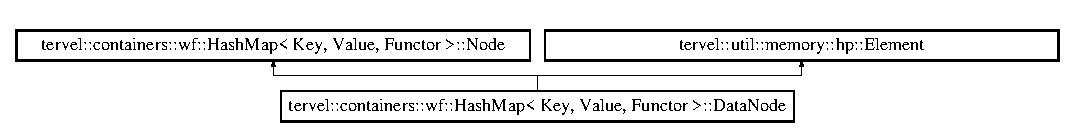
\includegraphics[height=1.403509cm]{classtervel_1_1containers_1_1wf_1_1_hash_map_1_1_data_node}
\end{center}
\end{figure}
\subsection*{Public Member Functions}
\begin{DoxyCompactItemize}
\item 
\hyperlink{classtervel_1_1containers_1_1wf_1_1_hash_map_1_1_data_node_ada4006f1254608301c4c19a08efc9f91}{Data\+Node} (Key k, \hyperlink{hash__map_2test_object_8h_ad777bf08d8e2b01df17ba5e3c51ae11f}{Value} v)
\item 
\hyperlink{classtervel_1_1containers_1_1wf_1_1_hash_map_1_1_data_node_afcd1913936c926974b4bfbe95c18559c}{$\sim$\+Data\+Node} ()
\item 
bool \hyperlink{classtervel_1_1containers_1_1wf_1_1_hash_map_1_1_data_node_a3b607ee5aaa378bd16f398c11708769e}{is\+\_\+array} ()
\item 
bool \hyperlink{classtervel_1_1containers_1_1wf_1_1_hash_map_1_1_data_node_a4a5c4a7e2de1b689d515d8d97322599d}{is\+\_\+data} ()
\end{DoxyCompactItemize}
\subsection*{Public Attributes}
\begin{DoxyCompactItemize}
\item 
Key \hyperlink{classtervel_1_1containers_1_1wf_1_1_hash_map_1_1_data_node_a261f271577727ee5699af49fdaaa989a}{key\+\_\+}
\item 
\hyperlink{hash__map_2test_object_8h_ad777bf08d8e2b01df17ba5e3c51ae11f}{Value} \hyperlink{classtervel_1_1containers_1_1wf_1_1_hash_map_1_1_data_node_a92498a88201109a8cababeff699435a6}{value\+\_\+}
\item 
std\+::atomic$<$ int64\+\_\+t $>$ \hyperlink{classtervel_1_1containers_1_1wf_1_1_hash_map_1_1_data_node_ab90537febd882ad210231df69691acae}{access\+\_\+count\+\_\+}
\end{DoxyCompactItemize}


\subsection{Detailed Description}
\subsubsection*{template$<$class Key, class Value, class Functor = default\+\_\+functor$<$\+Key, Value$>$$>$class tervel\+::containers\+::wf\+::\+Hash\+Map$<$ Key, Value, Functor $>$\+::\+Data\+Node}

This class is used to hold a key and value pair. 

It is hazard pointer protected. 

\subsection{Constructor \& Destructor Documentation}
\hypertarget{classtervel_1_1containers_1_1wf_1_1_hash_map_1_1_data_node_ada4006f1254608301c4c19a08efc9f91}{}\index{tervel\+::containers\+::wf\+::\+Hash\+Map\+::\+Data\+Node@{tervel\+::containers\+::wf\+::\+Hash\+Map\+::\+Data\+Node}!Data\+Node@{Data\+Node}}
\index{Data\+Node@{Data\+Node}!tervel\+::containers\+::wf\+::\+Hash\+Map\+::\+Data\+Node@{tervel\+::containers\+::wf\+::\+Hash\+Map\+::\+Data\+Node}}
\subsubsection[{Data\+Node(\+Key k, Value v)}]{\setlength{\rightskip}{0pt plus 5cm}template$<$class Key , class Value , class Functor  = default\+\_\+functor$<$\+Key, Value$>$$>$ {\bf tervel\+::containers\+::wf\+::\+Hash\+Map}$<$ Key, {\bf Value}, Functor $>$\+::Data\+Node\+::\+Data\+Node (
\begin{DoxyParamCaption}
\item[{Key}]{k, }
\item[{{\bf Value}}]{v}
\end{DoxyParamCaption}
)\hspace{0.3cm}{\ttfamily [inline]}, {\ttfamily [explicit]}}\label{classtervel_1_1containers_1_1wf_1_1_hash_map_1_1_data_node_ada4006f1254608301c4c19a08efc9f91}
\hypertarget{classtervel_1_1containers_1_1wf_1_1_hash_map_1_1_data_node_afcd1913936c926974b4bfbe95c18559c}{}\index{tervel\+::containers\+::wf\+::\+Hash\+Map\+::\+Data\+Node@{tervel\+::containers\+::wf\+::\+Hash\+Map\+::\+Data\+Node}!````~Data\+Node@{$\sim$\+Data\+Node}}
\index{````~Data\+Node@{$\sim$\+Data\+Node}!tervel\+::containers\+::wf\+::\+Hash\+Map\+::\+Data\+Node@{tervel\+::containers\+::wf\+::\+Hash\+Map\+::\+Data\+Node}}
\subsubsection[{$\sim$\+Data\+Node()}]{\setlength{\rightskip}{0pt plus 5cm}template$<$class Key , class Value , class Functor  = default\+\_\+functor$<$\+Key, Value$>$$>$ {\bf tervel\+::containers\+::wf\+::\+Hash\+Map}$<$ Key, {\bf Value}, Functor $>$\+::Data\+Node\+::$\sim$\+Data\+Node (
\begin{DoxyParamCaption}
{}
\end{DoxyParamCaption}
)\hspace{0.3cm}{\ttfamily [inline]}}\label{classtervel_1_1containers_1_1wf_1_1_hash_map_1_1_data_node_afcd1913936c926974b4bfbe95c18559c}


\subsection{Member Function Documentation}
\hypertarget{classtervel_1_1containers_1_1wf_1_1_hash_map_1_1_data_node_a3b607ee5aaa378bd16f398c11708769e}{}\index{tervel\+::containers\+::wf\+::\+Hash\+Map\+::\+Data\+Node@{tervel\+::containers\+::wf\+::\+Hash\+Map\+::\+Data\+Node}!is\+\_\+array@{is\+\_\+array}}
\index{is\+\_\+array@{is\+\_\+array}!tervel\+::containers\+::wf\+::\+Hash\+Map\+::\+Data\+Node@{tervel\+::containers\+::wf\+::\+Hash\+Map\+::\+Data\+Node}}
\subsubsection[{is\+\_\+array()}]{\setlength{\rightskip}{0pt plus 5cm}template$<$class Key , class Value , class Functor  = default\+\_\+functor$<$\+Key, Value$>$$>$ bool {\bf tervel\+::containers\+::wf\+::\+Hash\+Map}$<$ Key, {\bf Value}, Functor $>$\+::Data\+Node\+::is\+\_\+array (
\begin{DoxyParamCaption}
{}
\end{DoxyParamCaption}
)\hspace{0.3cm}{\ttfamily [inline]}, {\ttfamily [virtual]}}\label{classtervel_1_1containers_1_1wf_1_1_hash_map_1_1_data_node_a3b607ee5aaa378bd16f398c11708769e}
\begin{DoxyReturn}{Returns}
whether or not this instance is an Array\+Type sub type 
\end{DoxyReturn}


Implements \hyperlink{classtervel_1_1containers_1_1wf_1_1_hash_map_1_1_node_a0908bd3151f0b1b7f8fbb6825731fd15}{tervel\+::containers\+::wf\+::\+Hash\+Map$<$ Key, Value, Functor $>$\+::\+Node}.

\hypertarget{classtervel_1_1containers_1_1wf_1_1_hash_map_1_1_data_node_a4a5c4a7e2de1b689d515d8d97322599d}{}\index{tervel\+::containers\+::wf\+::\+Hash\+Map\+::\+Data\+Node@{tervel\+::containers\+::wf\+::\+Hash\+Map\+::\+Data\+Node}!is\+\_\+data@{is\+\_\+data}}
\index{is\+\_\+data@{is\+\_\+data}!tervel\+::containers\+::wf\+::\+Hash\+Map\+::\+Data\+Node@{tervel\+::containers\+::wf\+::\+Hash\+Map\+::\+Data\+Node}}
\subsubsection[{is\+\_\+data()}]{\setlength{\rightskip}{0pt plus 5cm}template$<$class Key , class Value , class Functor  = default\+\_\+functor$<$\+Key, Value$>$$>$ bool {\bf tervel\+::containers\+::wf\+::\+Hash\+Map}$<$ Key, {\bf Value}, Functor $>$\+::Data\+Node\+::is\+\_\+data (
\begin{DoxyParamCaption}
{}
\end{DoxyParamCaption}
)\hspace{0.3cm}{\ttfamily [inline]}, {\ttfamily [virtual]}}\label{classtervel_1_1containers_1_1wf_1_1_hash_map_1_1_data_node_a4a5c4a7e2de1b689d515d8d97322599d}
\begin{DoxyReturn}{Returns}
whether or not this instance is an \hyperlink{classtervel_1_1containers_1_1wf_1_1_hash_map_1_1_data_node}{Data\+Node} sub type 
\end{DoxyReturn}


Implements \hyperlink{classtervel_1_1containers_1_1wf_1_1_hash_map_1_1_node_ac7cc7039cfc134def7d936f00efc2155}{tervel\+::containers\+::wf\+::\+Hash\+Map$<$ Key, Value, Functor $>$\+::\+Node}.



\subsection{Member Data Documentation}
\hypertarget{classtervel_1_1containers_1_1wf_1_1_hash_map_1_1_data_node_ab90537febd882ad210231df69691acae}{}\index{tervel\+::containers\+::wf\+::\+Hash\+Map\+::\+Data\+Node@{tervel\+::containers\+::wf\+::\+Hash\+Map\+::\+Data\+Node}!access\+\_\+count\+\_\+@{access\+\_\+count\+\_\+}}
\index{access\+\_\+count\+\_\+@{access\+\_\+count\+\_\+}!tervel\+::containers\+::wf\+::\+Hash\+Map\+::\+Data\+Node@{tervel\+::containers\+::wf\+::\+Hash\+Map\+::\+Data\+Node}}
\subsubsection[{access\+\_\+count\+\_\+}]{\setlength{\rightskip}{0pt plus 5cm}template$<$class Key , class Value , class Functor  = default\+\_\+functor$<$\+Key, Value$>$$>$ std\+::atomic$<$int64\+\_\+t$>$ {\bf tervel\+::containers\+::wf\+::\+Hash\+Map}$<$ Key, {\bf Value}, Functor $>$\+::Data\+Node\+::access\+\_\+count\+\_\+}\label{classtervel_1_1containers_1_1wf_1_1_hash_map_1_1_data_node_ab90537febd882ad210231df69691acae}
\hypertarget{classtervel_1_1containers_1_1wf_1_1_hash_map_1_1_data_node_a261f271577727ee5699af49fdaaa989a}{}\index{tervel\+::containers\+::wf\+::\+Hash\+Map\+::\+Data\+Node@{tervel\+::containers\+::wf\+::\+Hash\+Map\+::\+Data\+Node}!key\+\_\+@{key\+\_\+}}
\index{key\+\_\+@{key\+\_\+}!tervel\+::containers\+::wf\+::\+Hash\+Map\+::\+Data\+Node@{tervel\+::containers\+::wf\+::\+Hash\+Map\+::\+Data\+Node}}
\subsubsection[{key\+\_\+}]{\setlength{\rightskip}{0pt plus 5cm}template$<$class Key , class Value , class Functor  = default\+\_\+functor$<$\+Key, Value$>$$>$ Key {\bf tervel\+::containers\+::wf\+::\+Hash\+Map}$<$ Key, {\bf Value}, Functor $>$\+::Data\+Node\+::key\+\_\+}\label{classtervel_1_1containers_1_1wf_1_1_hash_map_1_1_data_node_a261f271577727ee5699af49fdaaa989a}
\hypertarget{classtervel_1_1containers_1_1wf_1_1_hash_map_1_1_data_node_a92498a88201109a8cababeff699435a6}{}\index{tervel\+::containers\+::wf\+::\+Hash\+Map\+::\+Data\+Node@{tervel\+::containers\+::wf\+::\+Hash\+Map\+::\+Data\+Node}!value\+\_\+@{value\+\_\+}}
\index{value\+\_\+@{value\+\_\+}!tervel\+::containers\+::wf\+::\+Hash\+Map\+::\+Data\+Node@{tervel\+::containers\+::wf\+::\+Hash\+Map\+::\+Data\+Node}}
\subsubsection[{value\+\_\+}]{\setlength{\rightskip}{0pt plus 5cm}template$<$class Key , class Value , class Functor  = default\+\_\+functor$<$\+Key, Value$>$$>$ {\bf Value} {\bf tervel\+::containers\+::wf\+::\+Hash\+Map}$<$ Key, {\bf Value}, Functor $>$\+::Data\+Node\+::value\+\_\+}\label{classtervel_1_1containers_1_1wf_1_1_hash_map_1_1_data_node_a92498a88201109a8cababeff699435a6}


The documentation for this class was generated from the following file\+:\begin{DoxyCompactItemize}
\item 
tervel/containers/wf/hash-\/map/\hyperlink{wf__hash__map_8h}{wf\+\_\+hash\+\_\+map.\+h}\end{DoxyCompactItemize}

\hypertarget{classtervel_1_1containers_1_1wf_1_1_hash_map_no_delete_1_1_data_node}{}\section{tervel\+:\+:containers\+:\+:wf\+:\+:Hash\+Map\+No\+Delete$<$ Key, Value, Functor $>$\+:\+:Data\+Node Class Reference}
\label{classtervel_1_1containers_1_1wf_1_1_hash_map_no_delete_1_1_data_node}\index{tervel\+::containers\+::wf\+::\+Hash\+Map\+No\+Delete$<$ Key, Value, Functor $>$\+::\+Data\+Node@{tervel\+::containers\+::wf\+::\+Hash\+Map\+No\+Delete$<$ Key, Value, Functor $>$\+::\+Data\+Node}}


This class is used to hold a key and value pair.  


Inheritance diagram for tervel\+:\+:containers\+:\+:wf\+:\+:Hash\+Map\+No\+Delete$<$ Key, Value, Functor $>$\+:\+:Data\+Node\+:\begin{figure}[H]
\begin{center}
\leavevmode
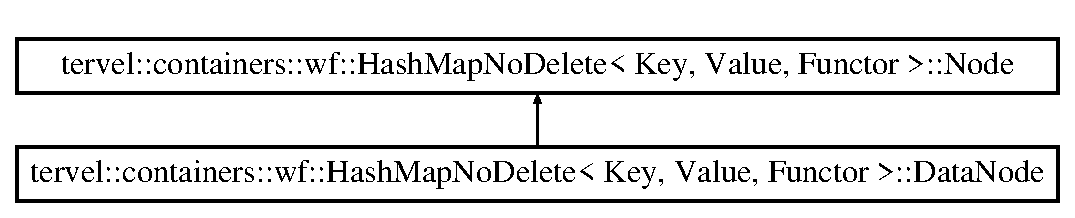
\includegraphics[height=2.000000cm]{classtervel_1_1containers_1_1wf_1_1_hash_map_no_delete_1_1_data_node}
\end{center}
\end{figure}
\subsection*{Public Member Functions}
\begin{DoxyCompactItemize}
\item 
\hyperlink{classtervel_1_1containers_1_1wf_1_1_hash_map_no_delete_1_1_data_node_a4cc9193f493ac699f609a8076eb47416}{Data\+Node} (Key k, \hyperlink{hash__map_2test_object_8h_ad777bf08d8e2b01df17ba5e3c51ae11f}{Value} v)
\item 
\hyperlink{classtervel_1_1containers_1_1wf_1_1_hash_map_no_delete_1_1_data_node_a52f4202ed5b4e8129e7820287bad90cd}{$\sim$\+Data\+Node} ()
\item 
bool \hyperlink{classtervel_1_1containers_1_1wf_1_1_hash_map_no_delete_1_1_data_node_a12ef4de7bec0bb237d2cb4f3eeab1a7d}{is\+\_\+array} ()
\item 
bool \hyperlink{classtervel_1_1containers_1_1wf_1_1_hash_map_no_delete_1_1_data_node_af8b10e3d6d939fd4655e92b884b160cf}{is\+\_\+data} ()
\end{DoxyCompactItemize}
\subsection*{Public Attributes}
\begin{DoxyCompactItemize}
\item 
Key \hyperlink{classtervel_1_1containers_1_1wf_1_1_hash_map_no_delete_1_1_data_node_af9ccfc5066e8ccc8c651e01f5968233e}{key\+\_\+}
\item 
\hyperlink{hash__map_2test_object_8h_ad777bf08d8e2b01df17ba5e3c51ae11f}{Value} \hyperlink{classtervel_1_1containers_1_1wf_1_1_hash_map_no_delete_1_1_data_node_a2f452c674e936fcfa45edee4b0416ea4}{value\+\_\+}
\end{DoxyCompactItemize}


\subsection{Detailed Description}
\subsubsection*{template$<$class Key, class Value, class Functor = default\+\_\+functor$<$\+Key, Value$>$$>$class tervel\+::containers\+::wf\+::\+Hash\+Map\+No\+Delete$<$ Key, Value, Functor $>$\+::\+Data\+Node}

This class is used to hold a key and value pair. 

It is hazard pointer protected. 

\subsection{Constructor \& Destructor Documentation}
\hypertarget{classtervel_1_1containers_1_1wf_1_1_hash_map_no_delete_1_1_data_node_a4cc9193f493ac699f609a8076eb47416}{}\index{tervel\+::containers\+::wf\+::\+Hash\+Map\+No\+Delete\+::\+Data\+Node@{tervel\+::containers\+::wf\+::\+Hash\+Map\+No\+Delete\+::\+Data\+Node}!Data\+Node@{Data\+Node}}
\index{Data\+Node@{Data\+Node}!tervel\+::containers\+::wf\+::\+Hash\+Map\+No\+Delete\+::\+Data\+Node@{tervel\+::containers\+::wf\+::\+Hash\+Map\+No\+Delete\+::\+Data\+Node}}
\subsubsection[{Data\+Node(\+Key k, Value v)}]{\setlength{\rightskip}{0pt plus 5cm}template$<$class Key , class Value , class Functor  = default\+\_\+functor$<$\+Key, Value$>$$>$ {\bf tervel\+::containers\+::wf\+::\+Hash\+Map\+No\+Delete}$<$ Key, {\bf Value}, Functor $>$\+::Data\+Node\+::\+Data\+Node (
\begin{DoxyParamCaption}
\item[{Key}]{k, }
\item[{{\bf Value}}]{v}
\end{DoxyParamCaption}
)\hspace{0.3cm}{\ttfamily [inline]}, {\ttfamily [explicit]}}\label{classtervel_1_1containers_1_1wf_1_1_hash_map_no_delete_1_1_data_node_a4cc9193f493ac699f609a8076eb47416}
\hypertarget{classtervel_1_1containers_1_1wf_1_1_hash_map_no_delete_1_1_data_node_a52f4202ed5b4e8129e7820287bad90cd}{}\index{tervel\+::containers\+::wf\+::\+Hash\+Map\+No\+Delete\+::\+Data\+Node@{tervel\+::containers\+::wf\+::\+Hash\+Map\+No\+Delete\+::\+Data\+Node}!````~Data\+Node@{$\sim$\+Data\+Node}}
\index{````~Data\+Node@{$\sim$\+Data\+Node}!tervel\+::containers\+::wf\+::\+Hash\+Map\+No\+Delete\+::\+Data\+Node@{tervel\+::containers\+::wf\+::\+Hash\+Map\+No\+Delete\+::\+Data\+Node}}
\subsubsection[{$\sim$\+Data\+Node()}]{\setlength{\rightskip}{0pt plus 5cm}template$<$class Key , class Value , class Functor  = default\+\_\+functor$<$\+Key, Value$>$$>$ {\bf tervel\+::containers\+::wf\+::\+Hash\+Map\+No\+Delete}$<$ Key, {\bf Value}, Functor $>$\+::Data\+Node\+::$\sim$\+Data\+Node (
\begin{DoxyParamCaption}
{}
\end{DoxyParamCaption}
)\hspace{0.3cm}{\ttfamily [inline]}}\label{classtervel_1_1containers_1_1wf_1_1_hash_map_no_delete_1_1_data_node_a52f4202ed5b4e8129e7820287bad90cd}


\subsection{Member Function Documentation}
\hypertarget{classtervel_1_1containers_1_1wf_1_1_hash_map_no_delete_1_1_data_node_a12ef4de7bec0bb237d2cb4f3eeab1a7d}{}\index{tervel\+::containers\+::wf\+::\+Hash\+Map\+No\+Delete\+::\+Data\+Node@{tervel\+::containers\+::wf\+::\+Hash\+Map\+No\+Delete\+::\+Data\+Node}!is\+\_\+array@{is\+\_\+array}}
\index{is\+\_\+array@{is\+\_\+array}!tervel\+::containers\+::wf\+::\+Hash\+Map\+No\+Delete\+::\+Data\+Node@{tervel\+::containers\+::wf\+::\+Hash\+Map\+No\+Delete\+::\+Data\+Node}}
\subsubsection[{is\+\_\+array()}]{\setlength{\rightskip}{0pt plus 5cm}template$<$class Key , class Value , class Functor  = default\+\_\+functor$<$\+Key, Value$>$$>$ bool {\bf tervel\+::containers\+::wf\+::\+Hash\+Map\+No\+Delete}$<$ Key, {\bf Value}, Functor $>$\+::Data\+Node\+::is\+\_\+array (
\begin{DoxyParamCaption}
{}
\end{DoxyParamCaption}
)\hspace{0.3cm}{\ttfamily [inline]}, {\ttfamily [virtual]}}\label{classtervel_1_1containers_1_1wf_1_1_hash_map_no_delete_1_1_data_node_a12ef4de7bec0bb237d2cb4f3eeab1a7d}
\begin{DoxyReturn}{Returns}
whether or not this instance is an Array\+Type sub type 
\end{DoxyReturn}


Implements \hyperlink{classtervel_1_1containers_1_1wf_1_1_hash_map_no_delete_1_1_node_a551c6b4900b06efe3fc1d4de7c25963b}{tervel\+::containers\+::wf\+::\+Hash\+Map\+No\+Delete$<$ Key, Value, Functor $>$\+::\+Node}.

\hypertarget{classtervel_1_1containers_1_1wf_1_1_hash_map_no_delete_1_1_data_node_af8b10e3d6d939fd4655e92b884b160cf}{}\index{tervel\+::containers\+::wf\+::\+Hash\+Map\+No\+Delete\+::\+Data\+Node@{tervel\+::containers\+::wf\+::\+Hash\+Map\+No\+Delete\+::\+Data\+Node}!is\+\_\+data@{is\+\_\+data}}
\index{is\+\_\+data@{is\+\_\+data}!tervel\+::containers\+::wf\+::\+Hash\+Map\+No\+Delete\+::\+Data\+Node@{tervel\+::containers\+::wf\+::\+Hash\+Map\+No\+Delete\+::\+Data\+Node}}
\subsubsection[{is\+\_\+data()}]{\setlength{\rightskip}{0pt plus 5cm}template$<$class Key , class Value , class Functor  = default\+\_\+functor$<$\+Key, Value$>$$>$ bool {\bf tervel\+::containers\+::wf\+::\+Hash\+Map\+No\+Delete}$<$ Key, {\bf Value}, Functor $>$\+::Data\+Node\+::is\+\_\+data (
\begin{DoxyParamCaption}
{}
\end{DoxyParamCaption}
)\hspace{0.3cm}{\ttfamily [inline]}, {\ttfamily [virtual]}}\label{classtervel_1_1containers_1_1wf_1_1_hash_map_no_delete_1_1_data_node_af8b10e3d6d939fd4655e92b884b160cf}
\begin{DoxyReturn}{Returns}
whether or not this instance is an \hyperlink{classtervel_1_1containers_1_1wf_1_1_hash_map_no_delete_1_1_data_node}{Data\+Node} sub type 
\end{DoxyReturn}


Implements \hyperlink{classtervel_1_1containers_1_1wf_1_1_hash_map_no_delete_1_1_node_a03ef6395f93104d0313296773be36b3c}{tervel\+::containers\+::wf\+::\+Hash\+Map\+No\+Delete$<$ Key, Value, Functor $>$\+::\+Node}.



\subsection{Member Data Documentation}
\hypertarget{classtervel_1_1containers_1_1wf_1_1_hash_map_no_delete_1_1_data_node_af9ccfc5066e8ccc8c651e01f5968233e}{}\index{tervel\+::containers\+::wf\+::\+Hash\+Map\+No\+Delete\+::\+Data\+Node@{tervel\+::containers\+::wf\+::\+Hash\+Map\+No\+Delete\+::\+Data\+Node}!key\+\_\+@{key\+\_\+}}
\index{key\+\_\+@{key\+\_\+}!tervel\+::containers\+::wf\+::\+Hash\+Map\+No\+Delete\+::\+Data\+Node@{tervel\+::containers\+::wf\+::\+Hash\+Map\+No\+Delete\+::\+Data\+Node}}
\subsubsection[{key\+\_\+}]{\setlength{\rightskip}{0pt plus 5cm}template$<$class Key , class Value , class Functor  = default\+\_\+functor$<$\+Key, Value$>$$>$ Key {\bf tervel\+::containers\+::wf\+::\+Hash\+Map\+No\+Delete}$<$ Key, {\bf Value}, Functor $>$\+::Data\+Node\+::key\+\_\+}\label{classtervel_1_1containers_1_1wf_1_1_hash_map_no_delete_1_1_data_node_af9ccfc5066e8ccc8c651e01f5968233e}
\hypertarget{classtervel_1_1containers_1_1wf_1_1_hash_map_no_delete_1_1_data_node_a2f452c674e936fcfa45edee4b0416ea4}{}\index{tervel\+::containers\+::wf\+::\+Hash\+Map\+No\+Delete\+::\+Data\+Node@{tervel\+::containers\+::wf\+::\+Hash\+Map\+No\+Delete\+::\+Data\+Node}!value\+\_\+@{value\+\_\+}}
\index{value\+\_\+@{value\+\_\+}!tervel\+::containers\+::wf\+::\+Hash\+Map\+No\+Delete\+::\+Data\+Node@{tervel\+::containers\+::wf\+::\+Hash\+Map\+No\+Delete\+::\+Data\+Node}}
\subsubsection[{value\+\_\+}]{\setlength{\rightskip}{0pt plus 5cm}template$<$class Key , class Value , class Functor  = default\+\_\+functor$<$\+Key, Value$>$$>$ {\bf Value} {\bf tervel\+::containers\+::wf\+::\+Hash\+Map\+No\+Delete}$<$ Key, {\bf Value}, Functor $>$\+::Data\+Node\+::value\+\_\+}\label{classtervel_1_1containers_1_1wf_1_1_hash_map_no_delete_1_1_data_node_a2f452c674e936fcfa45edee4b0416ea4}


The documentation for this class was generated from the following file\+:\begin{DoxyCompactItemize}
\item 
tervel/containers/wf/hash-\/map/\hyperlink{wf__hash__map__no__delete_8h}{wf\+\_\+hash\+\_\+map\+\_\+no\+\_\+delete.\+h}\end{DoxyCompactItemize}

\hypertarget{structtervel_1_1containers_1_1wf_1_1default__functor}{}\section{tervel\+:\+:containers\+:\+:wf\+:\+:default\+\_\+functor$<$ Key, Value $>$ Struct Template Reference}
\label{structtervel_1_1containers_1_1wf_1_1default__functor}\index{tervel\+::containers\+::wf\+::default\+\_\+functor$<$ Key, Value $>$@{tervel\+::containers\+::wf\+::default\+\_\+functor$<$ Key, Value $>$}}


A default Functor implementation.  




{\ttfamily \#include $<$wf\+\_\+hash\+\_\+map.\+h$>$}

\subsection*{Public Member Functions}
\begin{DoxyCompactItemize}
\item 
Key \hyperlink{structtervel_1_1containers_1_1wf_1_1default__functor_ad185cd085c0b61b6b82bd0faf9eda7ae}{hash} (Key k)
\item 
bool \hyperlink{structtervel_1_1containers_1_1wf_1_1default__functor_a7956a13bdb3ba082ac5e50800000254f}{key\+\_\+equals} (Key a, Key b)
\item 
Key \hyperlink{structtervel_1_1containers_1_1wf_1_1default__functor_ad185cd085c0b61b6b82bd0faf9eda7ae}{hash} (Key k)
\item 
bool \hyperlink{structtervel_1_1containers_1_1wf_1_1default__functor_a7956a13bdb3ba082ac5e50800000254f}{key\+\_\+equals} (Key a, Key b)
\end{DoxyCompactItemize}


\subsection{Detailed Description}
\subsubsection*{template$<$class Key, class Value$>$struct tervel\+::containers\+::wf\+::default\+\_\+functor$<$ Key, Value $>$}

A default Functor implementation. 



\subsection{Member Function Documentation}
\hypertarget{structtervel_1_1containers_1_1wf_1_1default__functor_ad185cd085c0b61b6b82bd0faf9eda7ae}{}\index{tervel\+::containers\+::wf\+::default\+\_\+functor@{tervel\+::containers\+::wf\+::default\+\_\+functor}!hash@{hash}}
\index{hash@{hash}!tervel\+::containers\+::wf\+::default\+\_\+functor@{tervel\+::containers\+::wf\+::default\+\_\+functor}}
\subsubsection[{hash(\+Key k)}]{\setlength{\rightskip}{0pt plus 5cm}template$<$class Key , class Value $>$ Key {\bf tervel\+::containers\+::wf\+::default\+\_\+functor}$<$ Key, {\bf Value} $>$\+::hash (
\begin{DoxyParamCaption}
\item[{Key}]{k}
\end{DoxyParamCaption}
)\hspace{0.3cm}{\ttfamily [inline]}}\label{structtervel_1_1containers_1_1wf_1_1default__functor_ad185cd085c0b61b6b82bd0faf9eda7ae}
\hypertarget{structtervel_1_1containers_1_1wf_1_1default__functor_ad185cd085c0b61b6b82bd0faf9eda7ae}{}\index{tervel\+::containers\+::wf\+::default\+\_\+functor@{tervel\+::containers\+::wf\+::default\+\_\+functor}!hash@{hash}}
\index{hash@{hash}!tervel\+::containers\+::wf\+::default\+\_\+functor@{tervel\+::containers\+::wf\+::default\+\_\+functor}}
\subsubsection[{hash(\+Key k)}]{\setlength{\rightskip}{0pt plus 5cm}template$<$class Key , class Value $>$ Key {\bf tervel\+::containers\+::wf\+::default\+\_\+functor}$<$ Key, {\bf Value} $>$\+::hash (
\begin{DoxyParamCaption}
\item[{Key}]{k}
\end{DoxyParamCaption}
)\hspace{0.3cm}{\ttfamily [inline]}}\label{structtervel_1_1containers_1_1wf_1_1default__functor_ad185cd085c0b61b6b82bd0faf9eda7ae}
\hypertarget{structtervel_1_1containers_1_1wf_1_1default__functor_a7956a13bdb3ba082ac5e50800000254f}{}\index{tervel\+::containers\+::wf\+::default\+\_\+functor@{tervel\+::containers\+::wf\+::default\+\_\+functor}!key\+\_\+equals@{key\+\_\+equals}}
\index{key\+\_\+equals@{key\+\_\+equals}!tervel\+::containers\+::wf\+::default\+\_\+functor@{tervel\+::containers\+::wf\+::default\+\_\+functor}}
\subsubsection[{key\+\_\+equals(\+Key a, Key b)}]{\setlength{\rightskip}{0pt plus 5cm}template$<$class Key , class Value $>$ bool {\bf tervel\+::containers\+::wf\+::default\+\_\+functor}$<$ Key, {\bf Value} $>$\+::key\+\_\+equals (
\begin{DoxyParamCaption}
\item[{Key}]{a, }
\item[{Key}]{b}
\end{DoxyParamCaption}
)\hspace{0.3cm}{\ttfamily [inline]}}\label{structtervel_1_1containers_1_1wf_1_1default__functor_a7956a13bdb3ba082ac5e50800000254f}
\hypertarget{structtervel_1_1containers_1_1wf_1_1default__functor_a7956a13bdb3ba082ac5e50800000254f}{}\index{tervel\+::containers\+::wf\+::default\+\_\+functor@{tervel\+::containers\+::wf\+::default\+\_\+functor}!key\+\_\+equals@{key\+\_\+equals}}
\index{key\+\_\+equals@{key\+\_\+equals}!tervel\+::containers\+::wf\+::default\+\_\+functor@{tervel\+::containers\+::wf\+::default\+\_\+functor}}
\subsubsection[{key\+\_\+equals(\+Key a, Key b)}]{\setlength{\rightskip}{0pt plus 5cm}template$<$class Key , class Value $>$ bool {\bf tervel\+::containers\+::wf\+::default\+\_\+functor}$<$ Key, {\bf Value} $>$\+::key\+\_\+equals (
\begin{DoxyParamCaption}
\item[{Key}]{a, }
\item[{Key}]{b}
\end{DoxyParamCaption}
)\hspace{0.3cm}{\ttfamily [inline]}}\label{structtervel_1_1containers_1_1wf_1_1default__functor_a7956a13bdb3ba082ac5e50800000254f}


The documentation for this struct was generated from the following files\+:\begin{DoxyCompactItemize}
\item 
tervel/containers/wf/hash-\/map/\hyperlink{wf__hash__map_8h}{wf\+\_\+hash\+\_\+map.\+h}\item 
tervel/containers/wf/hash-\/map/\hyperlink{wf__hash__map__no__delete_8h}{wf\+\_\+hash\+\_\+map\+\_\+no\+\_\+delete.\+h}\end{DoxyCompactItemize}

\hypertarget{classtervel_1_1containers_1_1wf_1_1_ring_buffer_1_1_dequeue_op}{}\section{tervel\+:\+:containers\+:\+:wf\+:\+:Ring\+Buffer$<$ T $>$\+:\+:Dequeue\+Op$<$ T $>$ Class Template Reference}
\label{classtervel_1_1containers_1_1wf_1_1_ring_buffer_1_1_dequeue_op}\index{tervel\+::containers\+::wf\+::\+Ring\+Buffer$<$ T $>$\+::\+Dequeue\+Op$<$ T $>$@{tervel\+::containers\+::wf\+::\+Ring\+Buffer$<$ T $>$\+::\+Dequeue\+Op$<$ T $>$}}


{\ttfamily \#include $<$dequeue\+\_\+op.\+h$>$}

Inheritance diagram for tervel\+:\+:containers\+:\+:wf\+:\+:Ring\+Buffer$<$ T $>$\+:\+:Dequeue\+Op$<$ T $>$\+:\begin{figure}[H]
\begin{center}
\leavevmode
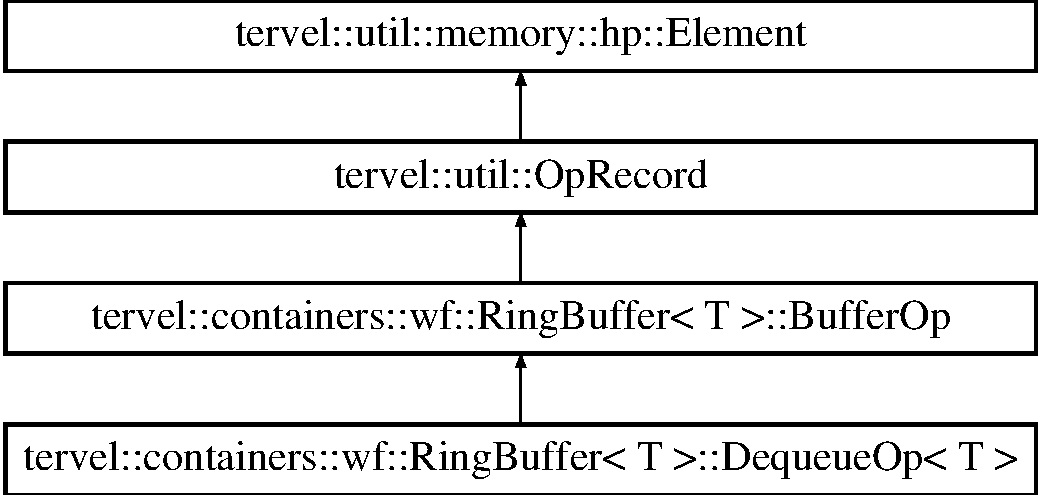
\includegraphics[height=4.000000cm]{classtervel_1_1containers_1_1wf_1_1_ring_buffer_1_1_dequeue_op}
\end{center}
\end{figure}
\subsection*{Public Member Functions}
\begin{DoxyCompactItemize}
\item 
\hyperlink{classtervel_1_1containers_1_1wf_1_1_ring_buffer_1_1_dequeue_op_ae05d7c29cc4e246da4c595bbecb52ae2}{Dequeue\+Op} (\hyperlink{classtervel_1_1containers_1_1wf_1_1_ring_buffer}{Ring\+Buffer}$<$ T $>$ $\ast$rb)
\item 
void $\ast$ \hyperlink{classtervel_1_1containers_1_1wf_1_1_ring_buffer_1_1_dequeue_op_a9c2398124db300ce3b28e3541e48d347}{associate} (\hyperlink{classtervel_1_1containers_1_1wf_1_1_ring_buffer_1_1_helper}{Helper} $\ast$h)
\item 
bool \hyperlink{classtervel_1_1containers_1_1wf_1_1_ring_buffer_1_1_dequeue_op_a87e54fafb11b49f95230ca72f035d20e}{result} (T \&val)
\item 
void \hyperlink{classtervel_1_1containers_1_1wf_1_1_ring_buffer_1_1_dequeue_op_a0f798edd2a65caf9ce112b496c27bdd5}{help\+\_\+complete} ()
\begin{DoxyCompactList}\small\item\em Implementations of this function that upon its return the operation described in the Op\+Record has been completed. \end{DoxyCompactList}\end{DoxyCompactItemize}
\subsection*{Private Member Functions}
\begin{DoxyCompactItemize}
\item 
\hyperlink{classtervel_1_1containers_1_1wf_1_1_ring_buffer_1_1_dequeue_op_af7083b776909fd8aa17cf7143c21cde7}{D\+I\+S\+A\+L\+L\+O\+W\+\_\+\+C\+O\+P\+Y\+\_\+\+A\+N\+D\+\_\+\+A\+S\+S\+I\+G\+N} (\hyperlink{classtervel_1_1containers_1_1wf_1_1_ring_buffer_1_1_dequeue_op}{Dequeue\+Op})
\end{DoxyCompactItemize}
\subsection*{Additional Inherited Members}


\subsection{Constructor \& Destructor Documentation}
\hypertarget{classtervel_1_1containers_1_1wf_1_1_ring_buffer_1_1_dequeue_op_ae05d7c29cc4e246da4c595bbecb52ae2}{}\index{tervel\+::containers\+::wf\+::\+Ring\+Buffer\+::\+Dequeue\+Op@{tervel\+::containers\+::wf\+::\+Ring\+Buffer\+::\+Dequeue\+Op}!Dequeue\+Op@{Dequeue\+Op}}
\index{Dequeue\+Op@{Dequeue\+Op}!tervel\+::containers\+::wf\+::\+Ring\+Buffer\+::\+Dequeue\+Op@{tervel\+::containers\+::wf\+::\+Ring\+Buffer\+::\+Dequeue\+Op}}
\subsubsection[{Dequeue\+Op(\+Ring\+Buffer$<$ T $>$ $\ast$rb)}]{\setlength{\rightskip}{0pt plus 5cm}template$<$typename T$>$ template$<$typename T $>$ {\bf tervel\+::containers\+::wf\+::\+Ring\+Buffer}$<$ T $>$\+::{\bf Dequeue\+Op}$<$ T $>$\+::{\bf Dequeue\+Op} (
\begin{DoxyParamCaption}
\item[{{\bf Ring\+Buffer}$<$ T $>$ $\ast$}]{rb}
\end{DoxyParamCaption}
)\hspace{0.3cm}{\ttfamily [inline]}}\label{classtervel_1_1containers_1_1wf_1_1_ring_buffer_1_1_dequeue_op_ae05d7c29cc4e246da4c595bbecb52ae2}


\subsection{Member Function Documentation}
\hypertarget{classtervel_1_1containers_1_1wf_1_1_ring_buffer_1_1_dequeue_op_a9c2398124db300ce3b28e3541e48d347}{}\index{tervel\+::containers\+::wf\+::\+Ring\+Buffer\+::\+Dequeue\+Op@{tervel\+::containers\+::wf\+::\+Ring\+Buffer\+::\+Dequeue\+Op}!associate@{associate}}
\index{associate@{associate}!tervel\+::containers\+::wf\+::\+Ring\+Buffer\+::\+Dequeue\+Op@{tervel\+::containers\+::wf\+::\+Ring\+Buffer\+::\+Dequeue\+Op}}
\subsubsection[{associate(\+Helper $\ast$h)}]{\setlength{\rightskip}{0pt plus 5cm}template$<$typename T$>$ template$<$typename T $>$ void $\ast$ {\bf tervel\+::containers\+::wf\+::\+Ring\+Buffer}$<$ T $>$\+::{\bf Dequeue\+Op}$<$ T $>$\+::associate (
\begin{DoxyParamCaption}
\item[{{\bf Helper} $\ast$}]{h}
\end{DoxyParamCaption}
)\hspace{0.3cm}{\ttfamily [virtual]}}\label{classtervel_1_1containers_1_1wf_1_1_ring_buffer_1_1_dequeue_op_a9c2398124db300ce3b28e3541e48d347}


Implements \hyperlink{classtervel_1_1containers_1_1wf_1_1_ring_buffer_1_1_buffer_op_a345d7432fa98f44f1620f5f718ff7a1e}{tervel\+::containers\+::wf\+::\+Ring\+Buffer$<$ T $>$\+::\+Buffer\+Op}.

\hypertarget{classtervel_1_1containers_1_1wf_1_1_ring_buffer_1_1_dequeue_op_af7083b776909fd8aa17cf7143c21cde7}{}\index{tervel\+::containers\+::wf\+::\+Ring\+Buffer\+::\+Dequeue\+Op@{tervel\+::containers\+::wf\+::\+Ring\+Buffer\+::\+Dequeue\+Op}!D\+I\+S\+A\+L\+L\+O\+W\+\_\+\+C\+O\+P\+Y\+\_\+\+A\+N\+D\+\_\+\+A\+S\+S\+I\+G\+N@{D\+I\+S\+A\+L\+L\+O\+W\+\_\+\+C\+O\+P\+Y\+\_\+\+A\+N\+D\+\_\+\+A\+S\+S\+I\+G\+N}}
\index{D\+I\+S\+A\+L\+L\+O\+W\+\_\+\+C\+O\+P\+Y\+\_\+\+A\+N\+D\+\_\+\+A\+S\+S\+I\+G\+N@{D\+I\+S\+A\+L\+L\+O\+W\+\_\+\+C\+O\+P\+Y\+\_\+\+A\+N\+D\+\_\+\+A\+S\+S\+I\+G\+N}!tervel\+::containers\+::wf\+::\+Ring\+Buffer\+::\+Dequeue\+Op@{tervel\+::containers\+::wf\+::\+Ring\+Buffer\+::\+Dequeue\+Op}}
\subsubsection[{D\+I\+S\+A\+L\+L\+O\+W\+\_\+\+C\+O\+P\+Y\+\_\+\+A\+N\+D\+\_\+\+A\+S\+S\+I\+G\+N(\+Dequeue\+Op)}]{\setlength{\rightskip}{0pt plus 5cm}template$<$typename T$>$ template$<$typename T $>$ {\bf tervel\+::containers\+::wf\+::\+Ring\+Buffer}$<$ T $>$\+::{\bf Dequeue\+Op}$<$ T $>$\+::D\+I\+S\+A\+L\+L\+O\+W\+\_\+\+C\+O\+P\+Y\+\_\+\+A\+N\+D\+\_\+\+A\+S\+S\+I\+G\+N (
\begin{DoxyParamCaption}
\item[{{\bf Dequeue\+Op}$<$ T $>$}]{}
\end{DoxyParamCaption}
)\hspace{0.3cm}{\ttfamily [private]}}\label{classtervel_1_1containers_1_1wf_1_1_ring_buffer_1_1_dequeue_op_af7083b776909fd8aa17cf7143c21cde7}
\hypertarget{classtervel_1_1containers_1_1wf_1_1_ring_buffer_1_1_dequeue_op_a0f798edd2a65caf9ce112b496c27bdd5}{}\index{tervel\+::containers\+::wf\+::\+Ring\+Buffer\+::\+Dequeue\+Op@{tervel\+::containers\+::wf\+::\+Ring\+Buffer\+::\+Dequeue\+Op}!help\+\_\+complete@{help\+\_\+complete}}
\index{help\+\_\+complete@{help\+\_\+complete}!tervel\+::containers\+::wf\+::\+Ring\+Buffer\+::\+Dequeue\+Op@{tervel\+::containers\+::wf\+::\+Ring\+Buffer\+::\+Dequeue\+Op}}
\subsubsection[{help\+\_\+complete()}]{\setlength{\rightskip}{0pt plus 5cm}template$<$typename T$>$ template$<$typename T $>$ void {\bf tervel\+::containers\+::wf\+::\+Ring\+Buffer}$<$ T $>$\+::{\bf Dequeue\+Op}$<$ T $>$\+::help\+\_\+complete (
\begin{DoxyParamCaption}
{}
\end{DoxyParamCaption}
)\hspace{0.3cm}{\ttfamily [virtual]}}\label{classtervel_1_1containers_1_1wf_1_1_ring_buffer_1_1_dequeue_op_a0f798edd2a65caf9ce112b496c27bdd5}


Implementations of this function that upon its return the operation described in the Op\+Record has been completed. 

As such it must be thread-\/safe and the extending class must contain all the information necessary to complete the operation. 

Implements \hyperlink{classtervel_1_1util_1_1_op_record_aa75ab39688a8d4cceb6a1ef0409537c0}{tervel\+::util\+::\+Op\+Record}.

\hypertarget{classtervel_1_1containers_1_1wf_1_1_ring_buffer_1_1_dequeue_op_a87e54fafb11b49f95230ca72f035d20e}{}\index{tervel\+::containers\+::wf\+::\+Ring\+Buffer\+::\+Dequeue\+Op@{tervel\+::containers\+::wf\+::\+Ring\+Buffer\+::\+Dequeue\+Op}!result@{result}}
\index{result@{result}!tervel\+::containers\+::wf\+::\+Ring\+Buffer\+::\+Dequeue\+Op@{tervel\+::containers\+::wf\+::\+Ring\+Buffer\+::\+Dequeue\+Op}}
\subsubsection[{result(\+T \&val)}]{\setlength{\rightskip}{0pt plus 5cm}template$<$typename T$>$ template$<$typename T $>$ bool {\bf tervel\+::containers\+::wf\+::\+Ring\+Buffer}$<$ T $>$\+::{\bf Dequeue\+Op}$<$ T $>$\+::result (
\begin{DoxyParamCaption}
\item[{T \&}]{val}
\end{DoxyParamCaption}
)}\label{classtervel_1_1containers_1_1wf_1_1_ring_buffer_1_1_dequeue_op_a87e54fafb11b49f95230ca72f035d20e}


The documentation for this class was generated from the following files\+:\begin{DoxyCompactItemize}
\item 
tervel/containers/wf/ring-\/buffer/\hyperlink{dequeue__op_8h}{dequeue\+\_\+op.\+h}\item 
tervel/containers/wf/ring-\/buffer/\hyperlink{dequeue__op__imp_8h}{dequeue\+\_\+op\+\_\+imp.\+h}\end{DoxyCompactItemize}

\hypertarget{classtervel_1_1util_1_1_descriptor}{}\section{tervel\+:\+:util\+:\+:Descriptor Class Reference}
\label{classtervel_1_1util_1_1_descriptor}\index{tervel\+::util\+::\+Descriptor@{tervel\+::util\+::\+Descriptor}}


This defines the \hyperlink{classtervel_1_1util_1_1_descriptor}{Descriptor} class, this class is designed to be extend and be used in conjunction with primarily the R\+C memory pool objects.  




{\ttfamily \#include $<$descriptor.\+h$>$}

Inheritance diagram for tervel\+:\+:util\+:\+:Descriptor\+:\begin{figure}[H]
\begin{center}
\leavevmode
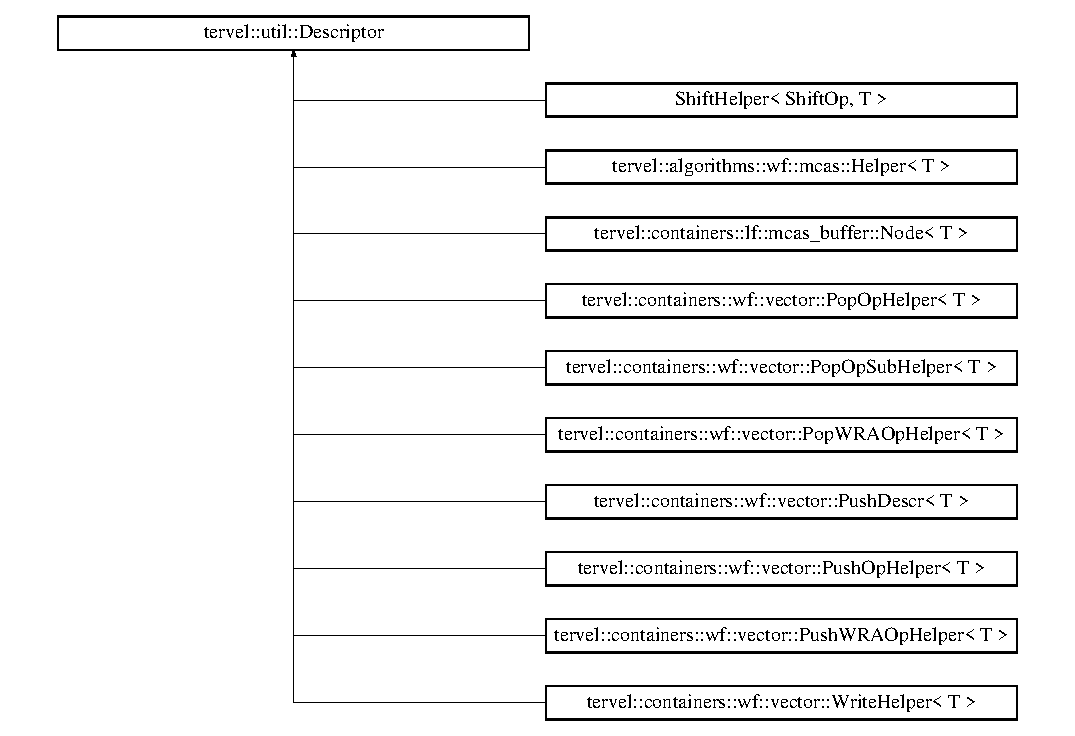
\includegraphics[height=9.447853cm]{classtervel_1_1util_1_1_descriptor}
\end{center}
\end{figure}
\subsection*{Public Member Functions}
\begin{DoxyCompactItemize}
\item 
\hyperlink{classtervel_1_1util_1_1_descriptor_a1c05a0355d92fbf9e48fb3be3b7de6a8}{Descriptor} ()
\item 
virtual \hyperlink{classtervel_1_1util_1_1_descriptor_a40ea2f979d8502d3d467d1a9ed5d770d}{$\sim$\+Descriptor} ()
\item 
virtual void $\ast$ \hyperlink{classtervel_1_1util_1_1_descriptor_a4303b2a08e3ab67de5533cfb20db87c9}{complete} (void $\ast$current, std\+::atomic$<$ void $\ast$ $>$ $\ast$address)=0
\begin{DoxyCompactList}\small\item\em This method is implemented by each sub class and must guarantee that upon return that the descriptor no longer exists at the address it was placed. \end{DoxyCompactList}\item 
virtual void $\ast$ \hyperlink{classtervel_1_1util_1_1_descriptor_a5b443eeb6acf1207f27a6d06c39d4ad4}{get\+\_\+logical\+\_\+value} ()=0
\begin{DoxyCompactList}\small\item\em This method is implemented by each sub class. \end{DoxyCompactList}\item 
virtual bool \hyperlink{classtervel_1_1util_1_1_descriptor_ab643e09f20f35149dc820766b0f9ccdb}{on\+\_\+watch} (std\+::atomic$<$ void $\ast$ $>$ $\ast$, void $\ast$)
\begin{DoxyCompactList}\small\item\em This method is optional to implement for each sub class. \end{DoxyCompactList}\item 
virtual void \hyperlink{classtervel_1_1util_1_1_descriptor_ad383c66e9e773acdf1533d3735617519}{on\+\_\+unwatch} ()
\begin{DoxyCompactList}\small\item\em This method must be implemented if on\+\_\+watch is implemented, and is optional otherwise. \end{DoxyCompactList}\item 
virtual bool \hyperlink{classtervel_1_1util_1_1_descriptor_ac419167492f68c1dc9e8bd517efe5e16}{on\+\_\+is\+\_\+watched} ()
\begin{DoxyCompactList}\small\item\em This method is optional to implement for each sub class. \end{DoxyCompactList}\end{DoxyCompactItemize}
\subsection*{Private Member Functions}
\begin{DoxyCompactItemize}
\item 
\hyperlink{classtervel_1_1util_1_1_descriptor_a9e8ac78761a5c86b66014a892ae52d36}{D\+I\+S\+A\+L\+L\+O\+W\+\_\+\+C\+O\+P\+Y\+\_\+\+A\+N\+D\+\_\+\+A\+S\+S\+I\+G\+N} (\hyperlink{classtervel_1_1util_1_1_descriptor}{Descriptor})
\end{DoxyCompactItemize}


\subsection{Detailed Description}
This defines the \hyperlink{classtervel_1_1util_1_1_descriptor}{Descriptor} class, this class is designed to be extend and be used in conjunction with primarily the R\+C memory pool objects. 

Extending this class allows the developer to quickly create R\+C protected elements.

Classes that extend this class must implement the following functions\+: complete get\+\_\+logical\+\_\+function. This allows for various algorithms and data structures to be executed on overlapping regions of memory.

For use with memory protection schemes we provide the following functions\+: on\+\_\+watch on\+\_\+is\+\_\+watched on\+\_\+unwatch These are called by the memory protection scheme in the event more advance logic is required to safely dereference of free such objects.

If an object contains a reference to other object(s) that can only be freed when it is freed then this must expressed in the objects destructor. 

\subsection{Constructor \& Destructor Documentation}
\hypertarget{classtervel_1_1util_1_1_descriptor_a1c05a0355d92fbf9e48fb3be3b7de6a8}{}\index{tervel\+::util\+::\+Descriptor@{tervel\+::util\+::\+Descriptor}!Descriptor@{Descriptor}}
\index{Descriptor@{Descriptor}!tervel\+::util\+::\+Descriptor@{tervel\+::util\+::\+Descriptor}}
\subsubsection[{Descriptor()}]{\setlength{\rightskip}{0pt plus 5cm}tervel\+::util\+::\+Descriptor\+::\+Descriptor (
\begin{DoxyParamCaption}
{}
\end{DoxyParamCaption}
)\hspace{0.3cm}{\ttfamily [inline]}}\label{classtervel_1_1util_1_1_descriptor_a1c05a0355d92fbf9e48fb3be3b7de6a8}
\hypertarget{classtervel_1_1util_1_1_descriptor_a40ea2f979d8502d3d467d1a9ed5d770d}{}\index{tervel\+::util\+::\+Descriptor@{tervel\+::util\+::\+Descriptor}!````~Descriptor@{$\sim$\+Descriptor}}
\index{````~Descriptor@{$\sim$\+Descriptor}!tervel\+::util\+::\+Descriptor@{tervel\+::util\+::\+Descriptor}}
\subsubsection[{$\sim$\+Descriptor()}]{\setlength{\rightskip}{0pt plus 5cm}virtual tervel\+::util\+::\+Descriptor\+::$\sim$\+Descriptor (
\begin{DoxyParamCaption}
{}
\end{DoxyParamCaption}
)\hspace{0.3cm}{\ttfamily [inline]}, {\ttfamily [virtual]}}\label{classtervel_1_1util_1_1_descriptor_a40ea2f979d8502d3d467d1a9ed5d770d}


\subsection{Member Function Documentation}
\hypertarget{classtervel_1_1util_1_1_descriptor_a4303b2a08e3ab67de5533cfb20db87c9}{}\index{tervel\+::util\+::\+Descriptor@{tervel\+::util\+::\+Descriptor}!complete@{complete}}
\index{complete@{complete}!tervel\+::util\+::\+Descriptor@{tervel\+::util\+::\+Descriptor}}
\subsubsection[{complete(void $\ast$current, std\+::atomic$<$ void $\ast$ $>$ $\ast$address)=0}]{\setlength{\rightskip}{0pt plus 5cm}virtual void$\ast$ tervel\+::util\+::\+Descriptor\+::complete (
\begin{DoxyParamCaption}
\item[{void $\ast$}]{current, }
\item[{std\+::atomic$<$ void $\ast$ $>$ $\ast$}]{address}
\end{DoxyParamCaption}
)\hspace{0.3cm}{\ttfamily [pure virtual]}}\label{classtervel_1_1util_1_1_descriptor_a4303b2a08e3ab67de5533cfb20db87c9}


This method is implemented by each sub class and must guarantee that upon return that the descriptor no longer exists at the address it was placed. 


\begin{DoxyParams}{Parameters}
{\em current} & the reference to this object as it is at the address, \\
\hline
{\em address} & the location this object was read from \\
\hline
\end{DoxyParams}


Implemented in \hyperlink{classtervel_1_1containers_1_1wf_1_1vector_1_1_pop_op_sub_helper_a8dc2729e8f7ed857c55df0f56361622b}{tervel\+::containers\+::wf\+::vector\+::\+Pop\+Op\+Sub\+Helper$<$ T $>$}, \hyperlink{classtervel_1_1containers_1_1wf_1_1vector_1_1_push_op_helper_a8faede3c50015027a4738b5a626c1ea6}{tervel\+::containers\+::wf\+::vector\+::\+Push\+Op\+Helper$<$ T $>$}, \hyperlink{classtervel_1_1containers_1_1wf_1_1vector_1_1_pop_op_helper_a1f92037dcfec837afe0684e119c7344f}{tervel\+::containers\+::wf\+::vector\+::\+Pop\+Op\+Helper$<$ T $>$}, \hyperlink{classtervel_1_1containers_1_1wf_1_1vector_1_1_push_descr_aa8d94d395ac24a37566dfdde8616ff53}{tervel\+::containers\+::wf\+::vector\+::\+Push\+Descr$<$ T $>$}, \hyperlink{classtervel_1_1containers_1_1wf_1_1vector_1_1_write_helper_a379b580d78358bf8332119541d8e87c0}{tervel\+::containers\+::wf\+::vector\+::\+Write\+Helper$<$ T $>$}, \hyperlink{classtervel_1_1containers_1_1wf_1_1vector_1_1_pop_w_r_a_op_helper_a4bb595dabd2cb32dc4171d82532c3413}{tervel\+::containers\+::wf\+::vector\+::\+Pop\+W\+R\+A\+Op\+Helper$<$ T $>$}, \hyperlink{classtervel_1_1containers_1_1wf_1_1vector_1_1_push_w_r_a_op_helper_a77a582be1e79950c4de106e031d5fa1c}{tervel\+::containers\+::wf\+::vector\+::\+Push\+W\+R\+A\+Op\+Helper$<$ T $>$}, \hyperlink{classtervel_1_1algorithms_1_1wf_1_1mcas_1_1_helper_a952a74178febcf25e6f3fe6d3fd8f691}{tervel\+::algorithms\+::wf\+::mcas\+::\+Helper$<$ T $>$}, and \hyperlink{classtervel_1_1containers_1_1lf_1_1mcas__buffer_1_1_node_afee54ad05721b9418bae358383e31f89}{tervel\+::containers\+::lf\+::mcas\+\_\+buffer\+::\+Node$<$ T $>$}.

\hypertarget{classtervel_1_1util_1_1_descriptor_a9e8ac78761a5c86b66014a892ae52d36}{}\index{tervel\+::util\+::\+Descriptor@{tervel\+::util\+::\+Descriptor}!D\+I\+S\+A\+L\+L\+O\+W\+\_\+\+C\+O\+P\+Y\+\_\+\+A\+N\+D\+\_\+\+A\+S\+S\+I\+G\+N@{D\+I\+S\+A\+L\+L\+O\+W\+\_\+\+C\+O\+P\+Y\+\_\+\+A\+N\+D\+\_\+\+A\+S\+S\+I\+G\+N}}
\index{D\+I\+S\+A\+L\+L\+O\+W\+\_\+\+C\+O\+P\+Y\+\_\+\+A\+N\+D\+\_\+\+A\+S\+S\+I\+G\+N@{D\+I\+S\+A\+L\+L\+O\+W\+\_\+\+C\+O\+P\+Y\+\_\+\+A\+N\+D\+\_\+\+A\+S\+S\+I\+G\+N}!tervel\+::util\+::\+Descriptor@{tervel\+::util\+::\+Descriptor}}
\subsubsection[{D\+I\+S\+A\+L\+L\+O\+W\+\_\+\+C\+O\+P\+Y\+\_\+\+A\+N\+D\+\_\+\+A\+S\+S\+I\+G\+N(\+Descriptor)}]{\setlength{\rightskip}{0pt plus 5cm}tervel\+::util\+::\+Descriptor\+::\+D\+I\+S\+A\+L\+L\+O\+W\+\_\+\+C\+O\+P\+Y\+\_\+\+A\+N\+D\+\_\+\+A\+S\+S\+I\+G\+N (
\begin{DoxyParamCaption}
\item[{{\bf Descriptor}}]{}
\end{DoxyParamCaption}
)\hspace{0.3cm}{\ttfamily [private]}}\label{classtervel_1_1util_1_1_descriptor_a9e8ac78761a5c86b66014a892ae52d36}
\hypertarget{classtervel_1_1util_1_1_descriptor_a5b443eeb6acf1207f27a6d06c39d4ad4}{}\index{tervel\+::util\+::\+Descriptor@{tervel\+::util\+::\+Descriptor}!get\+\_\+logical\+\_\+value@{get\+\_\+logical\+\_\+value}}
\index{get\+\_\+logical\+\_\+value@{get\+\_\+logical\+\_\+value}!tervel\+::util\+::\+Descriptor@{tervel\+::util\+::\+Descriptor}}
\subsubsection[{get\+\_\+logical\+\_\+value()=0}]{\setlength{\rightskip}{0pt plus 5cm}virtual void$\ast$ tervel\+::util\+::\+Descriptor\+::get\+\_\+logical\+\_\+value (
\begin{DoxyParamCaption}
{}
\end{DoxyParamCaption}
)\hspace{0.3cm}{\ttfamily [pure virtual]}}\label{classtervel_1_1util_1_1_descriptor_a5b443eeb6acf1207f27a6d06c39d4ad4}


This method is implemented by each sub class. 

It returns the logical value of the past address. If the associated operation is still in progress then it will generally return the value that was replaced by this descriptor. Otherwise it will generally return the result of the operation for the specified address.

It can only be called from the static function which protects the object from being reused during the function. 

Implemented in \hyperlink{classtervel_1_1containers_1_1wf_1_1vector_1_1_pop_op_sub_helper_a2b908a6e906f82a63af7e662fd6407cd}{tervel\+::containers\+::wf\+::vector\+::\+Pop\+Op\+Sub\+Helper$<$ T $>$}, \hyperlink{classtervel_1_1containers_1_1wf_1_1vector_1_1_push_op_helper_aa8ba2c9d99007ae04325294413601cff}{tervel\+::containers\+::wf\+::vector\+::\+Push\+Op\+Helper$<$ T $>$}, \hyperlink{classtervel_1_1containers_1_1wf_1_1vector_1_1_pop_op_helper_a0cd831d37361277e4e212e56d453dd70}{tervel\+::containers\+::wf\+::vector\+::\+Pop\+Op\+Helper$<$ T $>$}, \hyperlink{classtervel_1_1containers_1_1wf_1_1vector_1_1_push_descr_ada1424d353cb887e5f6380f08d0e926a}{tervel\+::containers\+::wf\+::vector\+::\+Push\+Descr$<$ T $>$}, \hyperlink{classtervel_1_1containers_1_1wf_1_1vector_1_1_write_helper_ae2c93c4fb9304dd82c25f5d8d9b23487}{tervel\+::containers\+::wf\+::vector\+::\+Write\+Helper$<$ T $>$}, \hyperlink{classtervel_1_1containers_1_1wf_1_1vector_1_1_push_w_r_a_op_helper_a2c1c6135378bd516be4a147d7e9a61a5}{tervel\+::containers\+::wf\+::vector\+::\+Push\+W\+R\+A\+Op\+Helper$<$ T $>$}, \hyperlink{classtervel_1_1algorithms_1_1wf_1_1mcas_1_1_helper_ad7fbc9ead7553cb023b0ecec2eaf45d4}{tervel\+::algorithms\+::wf\+::mcas\+::\+Helper$<$ T $>$}, \hyperlink{classtervel_1_1containers_1_1lf_1_1mcas__buffer_1_1_node_aceb3488510a25751e9055f13505a6a7d}{tervel\+::containers\+::lf\+::mcas\+\_\+buffer\+::\+Node$<$ T $>$}, and \hyperlink{class_shift_helper_a4c58f2e7ae4ce7e86a38fea777b3ff2e}{Shift\+Helper$<$ Shift\+Op, T $>$}.

\hypertarget{classtervel_1_1util_1_1_descriptor_ac419167492f68c1dc9e8bd517efe5e16}{}\index{tervel\+::util\+::\+Descriptor@{tervel\+::util\+::\+Descriptor}!on\+\_\+is\+\_\+watched@{on\+\_\+is\+\_\+watched}}
\index{on\+\_\+is\+\_\+watched@{on\+\_\+is\+\_\+watched}!tervel\+::util\+::\+Descriptor@{tervel\+::util\+::\+Descriptor}}
\subsubsection[{on\+\_\+is\+\_\+watched()}]{\setlength{\rightskip}{0pt plus 5cm}virtual bool tervel\+::util\+::\+Descriptor\+::on\+\_\+is\+\_\+watched (
\begin{DoxyParamCaption}
{}
\end{DoxyParamCaption}
)\hspace{0.3cm}{\ttfamily [inline]}, {\ttfamily [virtual]}}\label{classtervel_1_1util_1_1_descriptor_ac419167492f68c1dc9e8bd517efe5e16}


This method is optional to implement for each sub class. 

This function must be implemented if on\+\_\+watch is implemented.

\begin{DoxyReturn}{Returns}
true if the item is watched by another thread 
\end{DoxyReturn}


Reimplemented in \hyperlink{classtervel_1_1containers_1_1wf_1_1vector_1_1_pop_op_helper_afc30533f275eb109ae847e0038404360}{tervel\+::containers\+::wf\+::vector\+::\+Pop\+Op\+Helper$<$ T $>$}.

\hypertarget{classtervel_1_1util_1_1_descriptor_ad383c66e9e773acdf1533d3735617519}{}\index{tervel\+::util\+::\+Descriptor@{tervel\+::util\+::\+Descriptor}!on\+\_\+unwatch@{on\+\_\+unwatch}}
\index{on\+\_\+unwatch@{on\+\_\+unwatch}!tervel\+::util\+::\+Descriptor@{tervel\+::util\+::\+Descriptor}}
\subsubsection[{on\+\_\+unwatch()}]{\setlength{\rightskip}{0pt plus 5cm}virtual void tervel\+::util\+::\+Descriptor\+::on\+\_\+unwatch (
\begin{DoxyParamCaption}
{}
\end{DoxyParamCaption}
)\hspace{0.3cm}{\ttfamily [inline]}, {\ttfamily [virtual]}}\label{classtervel_1_1util_1_1_descriptor_ad383c66e9e773acdf1533d3735617519}


This method must be implemented if on\+\_\+watch is implemented, and is optional otherwise. 

It must unwatch any object watched by on\+\_\+watch. It should not unwatch itself. It is called when this descriptor is unwatched. 

Reimplemented in \hyperlink{classtervel_1_1containers_1_1wf_1_1vector_1_1_pop_op_helper_a90ee1e07905e336a864184e96d04bf96}{tervel\+::containers\+::wf\+::vector\+::\+Pop\+Op\+Helper$<$ T $>$}.

\hypertarget{classtervel_1_1util_1_1_descriptor_ab643e09f20f35149dc820766b0f9ccdb}{}\index{tervel\+::util\+::\+Descriptor@{tervel\+::util\+::\+Descriptor}!on\+\_\+watch@{on\+\_\+watch}}
\index{on\+\_\+watch@{on\+\_\+watch}!tervel\+::util\+::\+Descriptor@{tervel\+::util\+::\+Descriptor}}
\subsubsection[{on\+\_\+watch(std\+::atomic$<$ void $\ast$ $>$ $\ast$, void $\ast$)}]{\setlength{\rightskip}{0pt plus 5cm}virtual bool tervel\+::util\+::\+Descriptor\+::on\+\_\+watch (
\begin{DoxyParamCaption}
\item[{std\+::atomic$<$ void $\ast$ $>$ $\ast$}]{, }
\item[{void $\ast$}]{}
\end{DoxyParamCaption}
)\hspace{0.3cm}{\ttfamily [inline]}, {\ttfamily [virtual]}}\label{classtervel_1_1util_1_1_descriptor_ab643e09f20f35149dc820766b0f9ccdb}


This method is optional to implement for each sub class. 

In the event there is a complex dependency between descriptor objects, where watching one implies performing other actions, such as watching a parent object, a developer will implement this function to encapsulate that logic

This function is called by the static watch function It should not watch itself.


\begin{DoxyParams}{Parameters}
{\em address} & The location to check. \\
\hline
{\em expected} & The expected value for that location\\
\hline
\end{DoxyParams}
\begin{DoxyReturn}{Returns}
true if successful, false otherwise 
\end{DoxyReturn}


Reimplemented in \hyperlink{classtervel_1_1containers_1_1wf_1_1vector_1_1_pop_op_sub_helper_ae0fcfb9527874f0b321b0fd48a295833}{tervel\+::containers\+::wf\+::vector\+::\+Pop\+Op\+Sub\+Helper$<$ T $>$}, \hyperlink{classtervel_1_1containers_1_1wf_1_1vector_1_1_push_op_helper_a26ce47d7b64eedcf1983508f5a60d5b7}{tervel\+::containers\+::wf\+::vector\+::\+Push\+Op\+Helper$<$ T $>$}, \hyperlink{classtervel_1_1containers_1_1wf_1_1vector_1_1_pop_op_helper_a2b421b2a3cb984bd94abe3ee254ac819}{tervel\+::containers\+::wf\+::vector\+::\+Pop\+Op\+Helper$<$ T $>$}, \hyperlink{classtervel_1_1containers_1_1wf_1_1vector_1_1_write_helper_a4c914b2218dfcfffaae66e85ff77e6df}{tervel\+::containers\+::wf\+::vector\+::\+Write\+Helper$<$ T $>$}, \hyperlink{classtervel_1_1containers_1_1wf_1_1vector_1_1_push_w_r_a_op_helper_ab330b531d19d3ef8c8b86e239ce22215}{tervel\+::containers\+::wf\+::vector\+::\+Push\+W\+R\+A\+Op\+Helper$<$ T $>$}, \hyperlink{classtervel_1_1algorithms_1_1wf_1_1mcas_1_1_helper_a381449ae3b9624302008a581610f76b5}{tervel\+::algorithms\+::wf\+::mcas\+::\+Helper$<$ T $>$}, and \hyperlink{class_shift_helper_ad7f8e39f62c9646ec5862df3ee1e5ab4}{Shift\+Helper$<$ Shift\+Op, T $>$}.



The documentation for this class was generated from the following file\+:\begin{DoxyCompactItemize}
\item 
tervel/util/\hyperlink{descriptor_8h}{descriptor.\+h}\end{DoxyCompactItemize}

\hypertarget{classtervel_1_1util_1_1memory_1_1rc_1_1_descriptor_pool}{}\section{tervel\+:\+:util\+:\+:memory\+:\+:rc\+:\+:Descriptor\+Pool Class Reference}
\label{classtervel_1_1util_1_1memory_1_1rc_1_1_descriptor_pool}\index{tervel\+::util\+::memory\+::rc\+::\+Descriptor\+Pool@{tervel\+::util\+::memory\+::rc\+::\+Descriptor\+Pool}}


Defines a pool of descriptor objects which is used to allocate descriptors and to store them while they are not safe to delete.  




{\ttfamily \#include $<$descriptor\+\_\+pool.\+h$>$}

\subsection*{Public Member Functions}
\begin{DoxyCompactItemize}
\item 
\hyperlink{classtervel_1_1util_1_1memory_1_1rc_1_1_descriptor_pool_a552444bec208a324258ef830fa45597d}{Descriptor\+Pool} (\hyperlink{classtervel_1_1util_1_1memory_1_1rc_1_1_pool_manager}{Pool\+Manager} $\ast$manager, uint64\+\_\+t pool\+\_\+id, int prefill=\hyperlink{util_8h_afd0fad68cb3234a00478ba61d879a895}{T\+E\+R\+V\+E\+L\+\_\+\+M\+E\+M\+\_\+\+R\+C\+\_\+\+M\+I\+N\+\_\+\+N\+O\+D\+E\+S})
\item 
\hyperlink{classtervel_1_1util_1_1memory_1_1rc_1_1_descriptor_pool_ac3e88ac0469b52e803f4f1991611f72e}{$\sim$\+Descriptor\+Pool} ()
\item 
void \hyperlink{classtervel_1_1util_1_1memory_1_1rc_1_1_descriptor_pool_a6d086ae584f1ce4b23ec0f3040503c7d}{reserve} (size\+\_\+t num\+\_\+descriptors=\hyperlink{util_8h_afd0fad68cb3234a00478ba61d879a895}{T\+E\+R\+V\+E\+L\+\_\+\+M\+E\+M\+\_\+\+R\+C\+\_\+\+M\+I\+N\+\_\+\+N\+O\+D\+E\+S})
\begin{DoxyCompactList}\small\item\em Allocates an extra {\ttfamily num\+\_\+descriptors} elements to the pool. \end{DoxyCompactList}\item 
{\footnotesize template$<$typename Descr\+Type , typename... Args $>$ }\\Descr\+Type $\ast$ \hyperlink{classtervel_1_1util_1_1memory_1_1rc_1_1_descriptor_pool_aeba4dbb575d67e4c2425e1b15c4b3f11}{get\+\_\+descriptor} (Args \&\&...args)
\begin{DoxyCompactList}\small\item\em Constructs and returns a descriptor. \end{DoxyCompactList}\item 
void \hyperlink{classtervel_1_1util_1_1memory_1_1rc_1_1_descriptor_pool_aa81862471eea9aeed3b04ecc503b9197}{free\+\_\+descriptor} (\hyperlink{classtervel_1_1util_1_1_descriptor}{tervel\+::util\+::\+Descriptor} $\ast$descr, bool dont\+\_\+check=false)
\begin{DoxyCompactList}\small\item\em Once a user is done with a descriptor, they should free it with this method. \end{DoxyCompactList}\end{DoxyCompactItemize}
\subsection*{Private Member Functions}
\begin{DoxyCompactItemize}
\item 
\hyperlink{classtervel_1_1util_1_1memory_1_1rc_1_1_pool_element}{Pool\+Element} $\ast$ \hyperlink{classtervel_1_1util_1_1memory_1_1rc_1_1_descriptor_pool_a6a96d2e2269fdf2b9f56bf4249f1ef24}{get\+\_\+from\+\_\+pool} (bool allocate\+\_\+new=true)
\begin{DoxyCompactList}\small\item\em Gets a free element. \end{DoxyCompactList}\item 
void \hyperlink{classtervel_1_1util_1_1memory_1_1rc_1_1_descriptor_pool_a768ce63acad7353b919e71c722f5fe30}{send\+\_\+safe\+\_\+to\+\_\+manager} ()
\begin{DoxyCompactList}\small\item\em Sends the elements from the safe pool to the corresponding safe pool in this pool\textquotesingle{}s manager. \end{DoxyCompactList}\item 
void \hyperlink{classtervel_1_1util_1_1memory_1_1rc_1_1_descriptor_pool_a3e869b61b3689ce58c8749016d380926}{send\+\_\+unsafe\+\_\+to\+\_\+manager} ()
\begin{DoxyCompactList}\small\item\em Sends the elements from the unsafe pool to the corresponding unsafe pool in this pool\textquotesingle{}s manager. \end{DoxyCompactList}\item 
void \hyperlink{classtervel_1_1util_1_1memory_1_1rc_1_1_descriptor_pool_a362beb1ef559ba40a64ca78ffca12cff}{offload} ()
\begin{DoxyCompactList}\small\item\em Sends a subset of the elements to the managers pool. \end{DoxyCompactList}\item 
void \hyperlink{classtervel_1_1util_1_1memory_1_1rc_1_1_descriptor_pool_a573585b4dd774585e2430970f8c1b3fb}{add\+\_\+to\+\_\+safe} (\hyperlink{classtervel_1_1util_1_1_descriptor}{tervel\+::util\+::\+Descriptor} $\ast$descr)
\begin{DoxyCompactList}\small\item\em Releases the descriptor back to the safe pool. \end{DoxyCompactList}\item 
void \hyperlink{classtervel_1_1util_1_1memory_1_1rc_1_1_descriptor_pool_aae0b2295f7166b40c9c748a5ed78f570}{add\+\_\+to\+\_\+unsafe} (\hyperlink{classtervel_1_1util_1_1_descriptor}{tervel\+::util\+::\+Descriptor} $\ast$descr)
\begin{DoxyCompactList}\small\item\em Releases the descriptor back to the unsafe pool. \end{DoxyCompactList}\item 
void \hyperlink{classtervel_1_1util_1_1memory_1_1rc_1_1_descriptor_pool_aff5201eac41e952363dab1e23949f629}{try\+\_\+clear\+\_\+unsafe\+\_\+pool} (bool dont\+\_\+check=false)
\begin{DoxyCompactList}\small\item\em Try to move elements from the unsafe pool to the safe pool. \end{DoxyCompactList}\item 
bool \hyperlink{classtervel_1_1util_1_1memory_1_1rc_1_1_descriptor_pool_a602d77f377890c6c32311d8764a616a5}{verify\+\_\+pool\+\_\+count} (\hyperlink{classtervel_1_1util_1_1memory_1_1rc_1_1_pool_element}{Pool\+Element} $\ast$pool, uint64\+\_\+t count)
\begin{DoxyCompactList}\small\item\em verifies that the length of the linked list matches the count \end{DoxyCompactList}\item 
\hyperlink{classtervel_1_1util_1_1memory_1_1rc_1_1_descriptor_pool_a1a47980d510a2178f37a1c44fb54be54}{D\+I\+S\+A\+L\+L\+O\+W\+\_\+\+C\+O\+P\+Y\+\_\+\+A\+N\+D\+\_\+\+A\+S\+S\+I\+G\+N} (\hyperlink{classtervel_1_1util_1_1memory_1_1rc_1_1_descriptor_pool}{Descriptor\+Pool})
\end{DoxyCompactItemize}
\subsection*{Private Attributes}
\begin{DoxyCompactItemize}
\item 
\hyperlink{classtervel_1_1util_1_1memory_1_1rc_1_1_pool_manager}{Pool\+Manager} $\ast$ \hyperlink{classtervel_1_1util_1_1memory_1_1rc_1_1_descriptor_pool_a571b9eb199df3356d66d3a8137ad9944}{manager\+\_\+}
\begin{DoxyCompactList}\small\item\em This pool\textquotesingle{}s manager. \end{DoxyCompactList}\item 
uint64\+\_\+t \hyperlink{classtervel_1_1util_1_1memory_1_1rc_1_1_descriptor_pool_adec7cbd5e692812b0aa0afefa04697d7}{pool\+\_\+id\+\_\+}
\begin{DoxyCompactList}\small\item\em The pool where excess elements are placed. \end{DoxyCompactList}\item 
\hyperlink{classtervel_1_1util_1_1memory_1_1rc_1_1_pool_element}{Pool\+Element} $\ast$ \hyperlink{classtervel_1_1util_1_1memory_1_1rc_1_1_descriptor_pool_a816f71722b9a18b007154e27bdb153bd}{safe\+\_\+pool\+\_\+} \{nullptr\}
\begin{DoxyCompactList}\small\item\em A linked list of pool elements. \end{DoxyCompactList}\item 
\hyperlink{classtervel_1_1util_1_1memory_1_1rc_1_1_pool_element}{Pool\+Element} $\ast$ \hyperlink{classtervel_1_1util_1_1memory_1_1rc_1_1_descriptor_pool_a850e99b50092270ccc5e8529cffe294b}{unsafe\+\_\+pool\+\_\+} \{nullptr\}
\begin{DoxyCompactList}\small\item\em A linked list of pool elements. \end{DoxyCompactList}\item 
uint64\+\_\+t \hyperlink{classtervel_1_1util_1_1memory_1_1rc_1_1_descriptor_pool_a121f3c807724ee68f21faf5e659c2cf7}{safe\+\_\+pool\+\_\+count\+\_\+} \{0\}
\begin{DoxyCompactList}\small\item\em Two counters used to track the number of elements in the linked list. \end{DoxyCompactList}\item 
uint64\+\_\+t \hyperlink{classtervel_1_1util_1_1memory_1_1rc_1_1_descriptor_pool_a8b8a73ac56132217ea75bd6f5d13ba98}{unsafe\+\_\+pool\+\_\+count\+\_\+} \{0\}
\end{DoxyCompactItemize}


\subsection{Detailed Description}
Defines a pool of descriptor objects which is used to allocate descriptors and to store them while they are not safe to delete. 

The pool is represented as two linked lists of descriptors\+: one for safe elements and one for unsafe elements. The safe pool is known to only contain items owned by the thread owning the \hyperlink{classtervel_1_1util_1_1memory_1_1rc_1_1_descriptor_pool}{Descriptor\+Pool} object, and the unsafe pool contains items where other threads may still hold references to them.

Further, the pool object has a parent who is shared amongst other threads. When a pool is to be destroyed, it sends its remaining elements to the parent, relinquishing ownership of said elements. A top-\/level pool has a null parent. At the moment, it only makes sense to have a single top-\/level parent representing the central pool for all threads, and several local pools for each thread. 

\subsection{Constructor \& Destructor Documentation}
\hypertarget{classtervel_1_1util_1_1memory_1_1rc_1_1_descriptor_pool_a552444bec208a324258ef830fa45597d}{}\index{tervel\+::util\+::memory\+::rc\+::\+Descriptor\+Pool@{tervel\+::util\+::memory\+::rc\+::\+Descriptor\+Pool}!Descriptor\+Pool@{Descriptor\+Pool}}
\index{Descriptor\+Pool@{Descriptor\+Pool}!tervel\+::util\+::memory\+::rc\+::\+Descriptor\+Pool@{tervel\+::util\+::memory\+::rc\+::\+Descriptor\+Pool}}
\subsubsection[{Descriptor\+Pool(\+Pool\+Manager $\ast$manager, uint64\+\_\+t pool\+\_\+id, int prefill=\+T\+E\+R\+V\+E\+L\+\_\+\+M\+E\+M\+\_\+\+R\+C\+\_\+\+M\+I\+N\+\_\+\+N\+O\+D\+E\+S)}]{\setlength{\rightskip}{0pt plus 5cm}tervel\+::util\+::memory\+::rc\+::\+Descriptor\+Pool\+::\+Descriptor\+Pool (
\begin{DoxyParamCaption}
\item[{{\bf Pool\+Manager} $\ast$}]{manager, }
\item[{uint64\+\_\+t}]{pool\+\_\+id, }
\item[{int}]{prefill = {\ttfamily {\bf T\+E\+R\+V\+E\+L\+\_\+\+M\+E\+M\+\_\+\+R\+C\+\_\+\+M\+I\+N\+\_\+\+N\+O\+D\+E\+S}}}
\end{DoxyParamCaption}
)\hspace{0.3cm}{\ttfamily [inline]}}\label{classtervel_1_1util_1_1memory_1_1rc_1_1_descriptor_pool_a552444bec208a324258ef830fa45597d}
\hypertarget{classtervel_1_1util_1_1memory_1_1rc_1_1_descriptor_pool_ac3e88ac0469b52e803f4f1991611f72e}{}\index{tervel\+::util\+::memory\+::rc\+::\+Descriptor\+Pool@{tervel\+::util\+::memory\+::rc\+::\+Descriptor\+Pool}!````~Descriptor\+Pool@{$\sim$\+Descriptor\+Pool}}
\index{````~Descriptor\+Pool@{$\sim$\+Descriptor\+Pool}!tervel\+::util\+::memory\+::rc\+::\+Descriptor\+Pool@{tervel\+::util\+::memory\+::rc\+::\+Descriptor\+Pool}}
\subsubsection[{$\sim$\+Descriptor\+Pool()}]{\setlength{\rightskip}{0pt plus 5cm}tervel\+::util\+::memory\+::rc\+::\+Descriptor\+Pool\+::$\sim$\+Descriptor\+Pool (
\begin{DoxyParamCaption}
{}
\end{DoxyParamCaption}
)\hspace{0.3cm}{\ttfamily [inline]}}\label{classtervel_1_1util_1_1memory_1_1rc_1_1_descriptor_pool_ac3e88ac0469b52e803f4f1991611f72e}


\subsection{Member Function Documentation}
\hypertarget{classtervel_1_1util_1_1memory_1_1rc_1_1_descriptor_pool_a573585b4dd774585e2430970f8c1b3fb}{}\index{tervel\+::util\+::memory\+::rc\+::\+Descriptor\+Pool@{tervel\+::util\+::memory\+::rc\+::\+Descriptor\+Pool}!add\+\_\+to\+\_\+safe@{add\+\_\+to\+\_\+safe}}
\index{add\+\_\+to\+\_\+safe@{add\+\_\+to\+\_\+safe}!tervel\+::util\+::memory\+::rc\+::\+Descriptor\+Pool@{tervel\+::util\+::memory\+::rc\+::\+Descriptor\+Pool}}
\subsubsection[{add\+\_\+to\+\_\+safe(tervel\+::util\+::\+Descriptor $\ast$descr)}]{\setlength{\rightskip}{0pt plus 5cm}void tervel\+::util\+::memory\+::rc\+::\+Descriptor\+Pool\+::add\+\_\+to\+\_\+safe (
\begin{DoxyParamCaption}
\item[{{\bf tervel\+::util\+::\+Descriptor} $\ast$}]{descr}
\end{DoxyParamCaption}
)\hspace{0.3cm}{\ttfamily [private]}}\label{classtervel_1_1util_1_1memory_1_1rc_1_1_descriptor_pool_a573585b4dd774585e2430970f8c1b3fb}


Releases the descriptor back to the safe pool. 

Caller relinquishes ownership of descriptor. It\textquotesingle{}s expected that the given descriptor was taken from this pool to begin with.

Adding a descriptor to the safe pool calls its \textquotesingle{}on\+\_\+return\+\_\+to\+\_\+pool\textquotesingle{} method and its destructor. \hypertarget{classtervel_1_1util_1_1memory_1_1rc_1_1_descriptor_pool_aae0b2295f7166b40c9c748a5ed78f570}{}\index{tervel\+::util\+::memory\+::rc\+::\+Descriptor\+Pool@{tervel\+::util\+::memory\+::rc\+::\+Descriptor\+Pool}!add\+\_\+to\+\_\+unsafe@{add\+\_\+to\+\_\+unsafe}}
\index{add\+\_\+to\+\_\+unsafe@{add\+\_\+to\+\_\+unsafe}!tervel\+::util\+::memory\+::rc\+::\+Descriptor\+Pool@{tervel\+::util\+::memory\+::rc\+::\+Descriptor\+Pool}}
\subsubsection[{add\+\_\+to\+\_\+unsafe(tervel\+::util\+::\+Descriptor $\ast$descr)}]{\setlength{\rightskip}{0pt plus 5cm}void tervel\+::util\+::memory\+::rc\+::\+Descriptor\+Pool\+::add\+\_\+to\+\_\+unsafe (
\begin{DoxyParamCaption}
\item[{{\bf tervel\+::util\+::\+Descriptor} $\ast$}]{descr}
\end{DoxyParamCaption}
)\hspace{0.3cm}{\ttfamily [private]}}\label{classtervel_1_1util_1_1memory_1_1rc_1_1_descriptor_pool_aae0b2295f7166b40c9c748a5ed78f570}


Releases the descriptor back to the unsafe pool. 

Caller relinquishes ownership of descriptor. It\textquotesingle{}s expected that the given descriptor was taken from this pool to begin with.

See notes on \hyperlink{classtervel_1_1util_1_1memory_1_1rc_1_1_descriptor_pool_a573585b4dd774585e2430970f8c1b3fb}{add\+\_\+to\+\_\+safe()} \hypertarget{classtervel_1_1util_1_1memory_1_1rc_1_1_descriptor_pool_a1a47980d510a2178f37a1c44fb54be54}{}\index{tervel\+::util\+::memory\+::rc\+::\+Descriptor\+Pool@{tervel\+::util\+::memory\+::rc\+::\+Descriptor\+Pool}!D\+I\+S\+A\+L\+L\+O\+W\+\_\+\+C\+O\+P\+Y\+\_\+\+A\+N\+D\+\_\+\+A\+S\+S\+I\+G\+N@{D\+I\+S\+A\+L\+L\+O\+W\+\_\+\+C\+O\+P\+Y\+\_\+\+A\+N\+D\+\_\+\+A\+S\+S\+I\+G\+N}}
\index{D\+I\+S\+A\+L\+L\+O\+W\+\_\+\+C\+O\+P\+Y\+\_\+\+A\+N\+D\+\_\+\+A\+S\+S\+I\+G\+N@{D\+I\+S\+A\+L\+L\+O\+W\+\_\+\+C\+O\+P\+Y\+\_\+\+A\+N\+D\+\_\+\+A\+S\+S\+I\+G\+N}!tervel\+::util\+::memory\+::rc\+::\+Descriptor\+Pool@{tervel\+::util\+::memory\+::rc\+::\+Descriptor\+Pool}}
\subsubsection[{D\+I\+S\+A\+L\+L\+O\+W\+\_\+\+C\+O\+P\+Y\+\_\+\+A\+N\+D\+\_\+\+A\+S\+S\+I\+G\+N(\+Descriptor\+Pool)}]{\setlength{\rightskip}{0pt plus 5cm}tervel\+::util\+::memory\+::rc\+::\+Descriptor\+Pool\+::\+D\+I\+S\+A\+L\+L\+O\+W\+\_\+\+C\+O\+P\+Y\+\_\+\+A\+N\+D\+\_\+\+A\+S\+S\+I\+G\+N (
\begin{DoxyParamCaption}
\item[{{\bf Descriptor\+Pool}}]{}
\end{DoxyParamCaption}
)\hspace{0.3cm}{\ttfamily [private]}}\label{classtervel_1_1util_1_1memory_1_1rc_1_1_descriptor_pool_a1a47980d510a2178f37a1c44fb54be54}
\hypertarget{classtervel_1_1util_1_1memory_1_1rc_1_1_descriptor_pool_aa81862471eea9aeed3b04ecc503b9197}{}\index{tervel\+::util\+::memory\+::rc\+::\+Descriptor\+Pool@{tervel\+::util\+::memory\+::rc\+::\+Descriptor\+Pool}!free\+\_\+descriptor@{free\+\_\+descriptor}}
\index{free\+\_\+descriptor@{free\+\_\+descriptor}!tervel\+::util\+::memory\+::rc\+::\+Descriptor\+Pool@{tervel\+::util\+::memory\+::rc\+::\+Descriptor\+Pool}}
\subsubsection[{free\+\_\+descriptor(tervel\+::util\+::\+Descriptor $\ast$descr, bool dont\+\_\+check=false)}]{\setlength{\rightskip}{0pt plus 5cm}void tervel\+::util\+::memory\+::rc\+::\+Descriptor\+Pool\+::free\+\_\+descriptor (
\begin{DoxyParamCaption}
\item[{{\bf tervel\+::util\+::\+Descriptor} $\ast$}]{descr, }
\item[{bool}]{dont\+\_\+check = {\ttfamily false}}
\end{DoxyParamCaption}
)}\label{classtervel_1_1util_1_1memory_1_1rc_1_1_descriptor_pool_aa81862471eea9aeed3b04ecc503b9197}


Once a user is done with a descriptor, they should free it with this method. 


\begin{DoxyParams}{Parameters}
{\em descr} & The descriptor to free. \\
\hline
{\em dont\+\_\+check} & Don\textquotesingle{}t check if the descriptor is being watched before freeing it. Use this flag if you know that no other thread has had access to this descriptor. \\
\hline
{\em pool} & the pool to use when freeing the descriptor. \\
\hline
\end{DoxyParams}
\hypertarget{classtervel_1_1util_1_1memory_1_1rc_1_1_descriptor_pool_aeba4dbb575d67e4c2425e1b15c4b3f11}{}\index{tervel\+::util\+::memory\+::rc\+::\+Descriptor\+Pool@{tervel\+::util\+::memory\+::rc\+::\+Descriptor\+Pool}!get\+\_\+descriptor@{get\+\_\+descriptor}}
\index{get\+\_\+descriptor@{get\+\_\+descriptor}!tervel\+::util\+::memory\+::rc\+::\+Descriptor\+Pool@{tervel\+::util\+::memory\+::rc\+::\+Descriptor\+Pool}}
\subsubsection[{get\+\_\+descriptor(\+Args \&\&...\+args)}]{\setlength{\rightskip}{0pt plus 5cm}template$<$typename Descr\+Type , typename... Args $>$ Descr\+Type $\ast$ tervel\+::util\+::memory\+::rc\+::\+Descriptor\+Pool\+::get\+\_\+descriptor (
\begin{DoxyParamCaption}
\item[{Args \&\&...}]{args}
\end{DoxyParamCaption}
)}\label{classtervel_1_1util_1_1memory_1_1rc_1_1_descriptor_pool_aeba4dbb575d67e4c2425e1b15c4b3f11}


Constructs and returns a descriptor. 

Arguments are forwarded to the constructor of the given descriptor type. User should call free\+\_\+descriptor on the returned pointer when they are done with it to avoid memory leaks. \hypertarget{classtervel_1_1util_1_1memory_1_1rc_1_1_descriptor_pool_a6a96d2e2269fdf2b9f56bf4249f1ef24}{}\index{tervel\+::util\+::memory\+::rc\+::\+Descriptor\+Pool@{tervel\+::util\+::memory\+::rc\+::\+Descriptor\+Pool}!get\+\_\+from\+\_\+pool@{get\+\_\+from\+\_\+pool}}
\index{get\+\_\+from\+\_\+pool@{get\+\_\+from\+\_\+pool}!tervel\+::util\+::memory\+::rc\+::\+Descriptor\+Pool@{tervel\+::util\+::memory\+::rc\+::\+Descriptor\+Pool}}
\subsubsection[{get\+\_\+from\+\_\+pool(bool allocate\+\_\+new=true)}]{\setlength{\rightskip}{0pt plus 5cm}{\bf Pool\+Element}$\ast$ tervel\+::util\+::memory\+::rc\+::\+Descriptor\+Pool\+::get\+\_\+from\+\_\+pool (
\begin{DoxyParamCaption}
\item[{bool}]{allocate\+\_\+new = {\ttfamily true}}
\end{DoxyParamCaption}
)\hspace{0.3cm}{\ttfamily [private]}}\label{classtervel_1_1util_1_1memory_1_1rc_1_1_descriptor_pool_a6a96d2e2269fdf2b9f56bf4249f1ef24}


Gets a free element. 

The local pool is checked for one first, then the manager if there are no local ones, and if all else fails, a new one is allocated using new.


\begin{DoxyParams}{Parameters}
{\em allocate\+\_\+new} & If true and there are no free elements to retrieve from the pool, a new one is allocated. Otherwise, nullptr is returned. \\
\hline
\end{DoxyParams}
\hypertarget{classtervel_1_1util_1_1memory_1_1rc_1_1_descriptor_pool_a362beb1ef559ba40a64ca78ffca12cff}{}\index{tervel\+::util\+::memory\+::rc\+::\+Descriptor\+Pool@{tervel\+::util\+::memory\+::rc\+::\+Descriptor\+Pool}!offload@{offload}}
\index{offload@{offload}!tervel\+::util\+::memory\+::rc\+::\+Descriptor\+Pool@{tervel\+::util\+::memory\+::rc\+::\+Descriptor\+Pool}}
\subsubsection[{offload()}]{\setlength{\rightskip}{0pt plus 5cm}void tervel\+::util\+::memory\+::rc\+::\+Descriptor\+Pool\+::offload (
\begin{DoxyParamCaption}
{}
\end{DoxyParamCaption}
)\hspace{0.3cm}{\ttfamily [private]}}\label{classtervel_1_1util_1_1memory_1_1rc_1_1_descriptor_pool_a362beb1ef559ba40a64ca78ffca12cff}


Sends a subset of the elements to the managers pool. 

\hypertarget{classtervel_1_1util_1_1memory_1_1rc_1_1_descriptor_pool_a6d086ae584f1ce4b23ec0f3040503c7d}{}\index{tervel\+::util\+::memory\+::rc\+::\+Descriptor\+Pool@{tervel\+::util\+::memory\+::rc\+::\+Descriptor\+Pool}!reserve@{reserve}}
\index{reserve@{reserve}!tervel\+::util\+::memory\+::rc\+::\+Descriptor\+Pool@{tervel\+::util\+::memory\+::rc\+::\+Descriptor\+Pool}}
\subsubsection[{reserve(size\+\_\+t num\+\_\+descriptors=\+T\+E\+R\+V\+E\+L\+\_\+\+M\+E\+M\+\_\+\+R\+C\+\_\+\+M\+I\+N\+\_\+\+N\+O\+D\+E\+S)}]{\setlength{\rightskip}{0pt plus 5cm}void tervel\+::util\+::memory\+::rc\+::\+Descriptor\+Pool\+::reserve (
\begin{DoxyParamCaption}
\item[{size\+\_\+t}]{num\+\_\+descriptors = {\ttfamily {\bf T\+E\+R\+V\+E\+L\+\_\+\+M\+E\+M\+\_\+\+R\+C\+\_\+\+M\+I\+N\+\_\+\+N\+O\+D\+E\+S}}}
\end{DoxyParamCaption}
)}\label{classtervel_1_1util_1_1memory_1_1rc_1_1_descriptor_pool_a6d086ae584f1ce4b23ec0f3040503c7d}


Allocates an extra {\ttfamily num\+\_\+descriptors} elements to the pool. 

\hypertarget{classtervel_1_1util_1_1memory_1_1rc_1_1_descriptor_pool_a768ce63acad7353b919e71c722f5fe30}{}\index{tervel\+::util\+::memory\+::rc\+::\+Descriptor\+Pool@{tervel\+::util\+::memory\+::rc\+::\+Descriptor\+Pool}!send\+\_\+safe\+\_\+to\+\_\+manager@{send\+\_\+safe\+\_\+to\+\_\+manager}}
\index{send\+\_\+safe\+\_\+to\+\_\+manager@{send\+\_\+safe\+\_\+to\+\_\+manager}!tervel\+::util\+::memory\+::rc\+::\+Descriptor\+Pool@{tervel\+::util\+::memory\+::rc\+::\+Descriptor\+Pool}}
\subsubsection[{send\+\_\+safe\+\_\+to\+\_\+manager()}]{\setlength{\rightskip}{0pt plus 5cm}void tervel\+::util\+::memory\+::rc\+::\+Descriptor\+Pool\+::send\+\_\+safe\+\_\+to\+\_\+manager (
\begin{DoxyParamCaption}
{}
\end{DoxyParamCaption}
)\hspace{0.3cm}{\ttfamily [private]}}\label{classtervel_1_1util_1_1memory_1_1rc_1_1_descriptor_pool_a768ce63acad7353b919e71c722f5fe30}


Sends the elements from the safe pool to the corresponding safe pool in this pool\textquotesingle{}s manager. 

\hypertarget{classtervel_1_1util_1_1memory_1_1rc_1_1_descriptor_pool_a3e869b61b3689ce58c8749016d380926}{}\index{tervel\+::util\+::memory\+::rc\+::\+Descriptor\+Pool@{tervel\+::util\+::memory\+::rc\+::\+Descriptor\+Pool}!send\+\_\+unsafe\+\_\+to\+\_\+manager@{send\+\_\+unsafe\+\_\+to\+\_\+manager}}
\index{send\+\_\+unsafe\+\_\+to\+\_\+manager@{send\+\_\+unsafe\+\_\+to\+\_\+manager}!tervel\+::util\+::memory\+::rc\+::\+Descriptor\+Pool@{tervel\+::util\+::memory\+::rc\+::\+Descriptor\+Pool}}
\subsubsection[{send\+\_\+unsafe\+\_\+to\+\_\+manager()}]{\setlength{\rightskip}{0pt plus 5cm}void tervel\+::util\+::memory\+::rc\+::\+Descriptor\+Pool\+::send\+\_\+unsafe\+\_\+to\+\_\+manager (
\begin{DoxyParamCaption}
{}
\end{DoxyParamCaption}
)\hspace{0.3cm}{\ttfamily [private]}}\label{classtervel_1_1util_1_1memory_1_1rc_1_1_descriptor_pool_a3e869b61b3689ce58c8749016d380926}


Sends the elements from the unsafe pool to the corresponding unsafe pool in this pool\textquotesingle{}s manager. 

\hypertarget{classtervel_1_1util_1_1memory_1_1rc_1_1_descriptor_pool_aff5201eac41e952363dab1e23949f629}{}\index{tervel\+::util\+::memory\+::rc\+::\+Descriptor\+Pool@{tervel\+::util\+::memory\+::rc\+::\+Descriptor\+Pool}!try\+\_\+clear\+\_\+unsafe\+\_\+pool@{try\+\_\+clear\+\_\+unsafe\+\_\+pool}}
\index{try\+\_\+clear\+\_\+unsafe\+\_\+pool@{try\+\_\+clear\+\_\+unsafe\+\_\+pool}!tervel\+::util\+::memory\+::rc\+::\+Descriptor\+Pool@{tervel\+::util\+::memory\+::rc\+::\+Descriptor\+Pool}}
\subsubsection[{try\+\_\+clear\+\_\+unsafe\+\_\+pool(bool dont\+\_\+check=false)}]{\setlength{\rightskip}{0pt plus 5cm}void tervel\+::util\+::memory\+::rc\+::\+Descriptor\+Pool\+::try\+\_\+clear\+\_\+unsafe\+\_\+pool (
\begin{DoxyParamCaption}
\item[{bool}]{dont\+\_\+check = {\ttfamily false}}
\end{DoxyParamCaption}
)\hspace{0.3cm}{\ttfamily [private]}}\label{classtervel_1_1util_1_1memory_1_1rc_1_1_descriptor_pool_aff5201eac41e952363dab1e23949f629}


Try to move elements from the unsafe pool to the safe pool. 

\hypertarget{classtervel_1_1util_1_1memory_1_1rc_1_1_descriptor_pool_a602d77f377890c6c32311d8764a616a5}{}\index{tervel\+::util\+::memory\+::rc\+::\+Descriptor\+Pool@{tervel\+::util\+::memory\+::rc\+::\+Descriptor\+Pool}!verify\+\_\+pool\+\_\+count@{verify\+\_\+pool\+\_\+count}}
\index{verify\+\_\+pool\+\_\+count@{verify\+\_\+pool\+\_\+count}!tervel\+::util\+::memory\+::rc\+::\+Descriptor\+Pool@{tervel\+::util\+::memory\+::rc\+::\+Descriptor\+Pool}}
\subsubsection[{verify\+\_\+pool\+\_\+count(\+Pool\+Element $\ast$pool, uint64\+\_\+t count)}]{\setlength{\rightskip}{0pt plus 5cm}bool tervel\+::util\+::memory\+::rc\+::\+Descriptor\+Pool\+::verify\+\_\+pool\+\_\+count (
\begin{DoxyParamCaption}
\item[{{\bf Pool\+Element} $\ast$}]{pool, }
\item[{uint64\+\_\+t}]{count}
\end{DoxyParamCaption}
)\hspace{0.3cm}{\ttfamily [private]}}\label{classtervel_1_1util_1_1memory_1_1rc_1_1_descriptor_pool_a602d77f377890c6c32311d8764a616a5}


verifies that the length of the linked list matches the count 



\subsection{Member Data Documentation}
\hypertarget{classtervel_1_1util_1_1memory_1_1rc_1_1_descriptor_pool_a571b9eb199df3356d66d3a8137ad9944}{}\index{tervel\+::util\+::memory\+::rc\+::\+Descriptor\+Pool@{tervel\+::util\+::memory\+::rc\+::\+Descriptor\+Pool}!manager\+\_\+@{manager\+\_\+}}
\index{manager\+\_\+@{manager\+\_\+}!tervel\+::util\+::memory\+::rc\+::\+Descriptor\+Pool@{tervel\+::util\+::memory\+::rc\+::\+Descriptor\+Pool}}
\subsubsection[{manager\+\_\+}]{\setlength{\rightskip}{0pt plus 5cm}{\bf Pool\+Manager}$\ast$ tervel\+::util\+::memory\+::rc\+::\+Descriptor\+Pool\+::manager\+\_\+\hspace{0.3cm}{\ttfamily [private]}}\label{classtervel_1_1util_1_1memory_1_1rc_1_1_descriptor_pool_a571b9eb199df3356d66d3a8137ad9944}


This pool\textquotesingle{}s manager. 

\hypertarget{classtervel_1_1util_1_1memory_1_1rc_1_1_descriptor_pool_adec7cbd5e692812b0aa0afefa04697d7}{}\index{tervel\+::util\+::memory\+::rc\+::\+Descriptor\+Pool@{tervel\+::util\+::memory\+::rc\+::\+Descriptor\+Pool}!pool\+\_\+id\+\_\+@{pool\+\_\+id\+\_\+}}
\index{pool\+\_\+id\+\_\+@{pool\+\_\+id\+\_\+}!tervel\+::util\+::memory\+::rc\+::\+Descriptor\+Pool@{tervel\+::util\+::memory\+::rc\+::\+Descriptor\+Pool}}
\subsubsection[{pool\+\_\+id\+\_\+}]{\setlength{\rightskip}{0pt plus 5cm}uint64\+\_\+t tervel\+::util\+::memory\+::rc\+::\+Descriptor\+Pool\+::pool\+\_\+id\+\_\+\hspace{0.3cm}{\ttfamily [private]}}\label{classtervel_1_1util_1_1memory_1_1rc_1_1_descriptor_pool_adec7cbd5e692812b0aa0afefa04697d7}


The pool where excess elements are placed. 

\hypertarget{classtervel_1_1util_1_1memory_1_1rc_1_1_descriptor_pool_a816f71722b9a18b007154e27bdb153bd}{}\index{tervel\+::util\+::memory\+::rc\+::\+Descriptor\+Pool@{tervel\+::util\+::memory\+::rc\+::\+Descriptor\+Pool}!safe\+\_\+pool\+\_\+@{safe\+\_\+pool\+\_\+}}
\index{safe\+\_\+pool\+\_\+@{safe\+\_\+pool\+\_\+}!tervel\+::util\+::memory\+::rc\+::\+Descriptor\+Pool@{tervel\+::util\+::memory\+::rc\+::\+Descriptor\+Pool}}
\subsubsection[{safe\+\_\+pool\+\_\+}]{\setlength{\rightskip}{0pt plus 5cm}{\bf Pool\+Element}$\ast$ tervel\+::util\+::memory\+::rc\+::\+Descriptor\+Pool\+::safe\+\_\+pool\+\_\+ \{nullptr\}\hspace{0.3cm}{\ttfamily [private]}}\label{classtervel_1_1util_1_1memory_1_1rc_1_1_descriptor_pool_a816f71722b9a18b007154e27bdb153bd}


A linked list of pool elements. 

One can be assured that no thread will try to access the descriptor of any element in this pool. They can\textquotesingle{}t be freed as some threads may still have access to the element itself and may try to increment the refrence count. \hypertarget{classtervel_1_1util_1_1memory_1_1rc_1_1_descriptor_pool_a121f3c807724ee68f21faf5e659c2cf7}{}\index{tervel\+::util\+::memory\+::rc\+::\+Descriptor\+Pool@{tervel\+::util\+::memory\+::rc\+::\+Descriptor\+Pool}!safe\+\_\+pool\+\_\+count\+\_\+@{safe\+\_\+pool\+\_\+count\+\_\+}}
\index{safe\+\_\+pool\+\_\+count\+\_\+@{safe\+\_\+pool\+\_\+count\+\_\+}!tervel\+::util\+::memory\+::rc\+::\+Descriptor\+Pool@{tervel\+::util\+::memory\+::rc\+::\+Descriptor\+Pool}}
\subsubsection[{safe\+\_\+pool\+\_\+count\+\_\+}]{\setlength{\rightskip}{0pt plus 5cm}uint64\+\_\+t tervel\+::util\+::memory\+::rc\+::\+Descriptor\+Pool\+::safe\+\_\+pool\+\_\+count\+\_\+ \{0\}\hspace{0.3cm}{\ttfamily [private]}}\label{classtervel_1_1util_1_1memory_1_1rc_1_1_descriptor_pool_a121f3c807724ee68f21faf5e659c2cf7}


Two counters used to track the number of elements in the linked list. 

this facilitates the detection of when there are too many elements. \hypertarget{classtervel_1_1util_1_1memory_1_1rc_1_1_descriptor_pool_a850e99b50092270ccc5e8529cffe294b}{}\index{tervel\+::util\+::memory\+::rc\+::\+Descriptor\+Pool@{tervel\+::util\+::memory\+::rc\+::\+Descriptor\+Pool}!unsafe\+\_\+pool\+\_\+@{unsafe\+\_\+pool\+\_\+}}
\index{unsafe\+\_\+pool\+\_\+@{unsafe\+\_\+pool\+\_\+}!tervel\+::util\+::memory\+::rc\+::\+Descriptor\+Pool@{tervel\+::util\+::memory\+::rc\+::\+Descriptor\+Pool}}
\subsubsection[{unsafe\+\_\+pool\+\_\+}]{\setlength{\rightskip}{0pt plus 5cm}{\bf Pool\+Element}$\ast$ tervel\+::util\+::memory\+::rc\+::\+Descriptor\+Pool\+::unsafe\+\_\+pool\+\_\+ \{nullptr\}\hspace{0.3cm}{\ttfamily [private]}}\label{classtervel_1_1util_1_1memory_1_1rc_1_1_descriptor_pool_a850e99b50092270ccc5e8529cffe294b}


A linked list of pool elements. 

Elements get released to this pool when they\textquotesingle{}re no longer needed, but some threads may still try to access the descriptor in the element. After some time has passed, items generally move from this pool to the safe\+\_\+pool\+\_\+ \hypertarget{classtervel_1_1util_1_1memory_1_1rc_1_1_descriptor_pool_a8b8a73ac56132217ea75bd6f5d13ba98}{}\index{tervel\+::util\+::memory\+::rc\+::\+Descriptor\+Pool@{tervel\+::util\+::memory\+::rc\+::\+Descriptor\+Pool}!unsafe\+\_\+pool\+\_\+count\+\_\+@{unsafe\+\_\+pool\+\_\+count\+\_\+}}
\index{unsafe\+\_\+pool\+\_\+count\+\_\+@{unsafe\+\_\+pool\+\_\+count\+\_\+}!tervel\+::util\+::memory\+::rc\+::\+Descriptor\+Pool@{tervel\+::util\+::memory\+::rc\+::\+Descriptor\+Pool}}
\subsubsection[{unsafe\+\_\+pool\+\_\+count\+\_\+}]{\setlength{\rightskip}{0pt plus 5cm}uint64\+\_\+t tervel\+::util\+::memory\+::rc\+::\+Descriptor\+Pool\+::unsafe\+\_\+pool\+\_\+count\+\_\+ \{0\}\hspace{0.3cm}{\ttfamily [private]}}\label{classtervel_1_1util_1_1memory_1_1rc_1_1_descriptor_pool_a8b8a73ac56132217ea75bd6f5d13ba98}


The documentation for this class was generated from the following file\+:\begin{DoxyCompactItemize}
\item 
tervel/util/memory/rc/\hyperlink{descriptor__pool_8h}{descriptor\+\_\+pool.\+h}\end{DoxyCompactItemize}

\hypertarget{classtervel_1_1util_1_1memory_1_1hp_1_1_element}{}\section{tervel\+:\+:util\+:\+:memory\+:\+:hp\+:\+:Element Class Reference}
\label{classtervel_1_1util_1_1memory_1_1hp_1_1_element}\index{tervel\+::util\+::memory\+::hp\+::\+Element@{tervel\+::util\+::memory\+::hp\+::\+Element}}


This class is used for the creation of Hazard Pointer Protected Objects Objects which extend it have the ability to call safe\+Free which delays the calling of the objects destructor until it is safe to do so.  




{\ttfamily \#include $<$hp\+\_\+element.\+h$>$}

Inheritance diagram for tervel\+:\+:util\+:\+:memory\+:\+:hp\+:\+:Element\+:\begin{figure}[H]
\begin{center}
\leavevmode
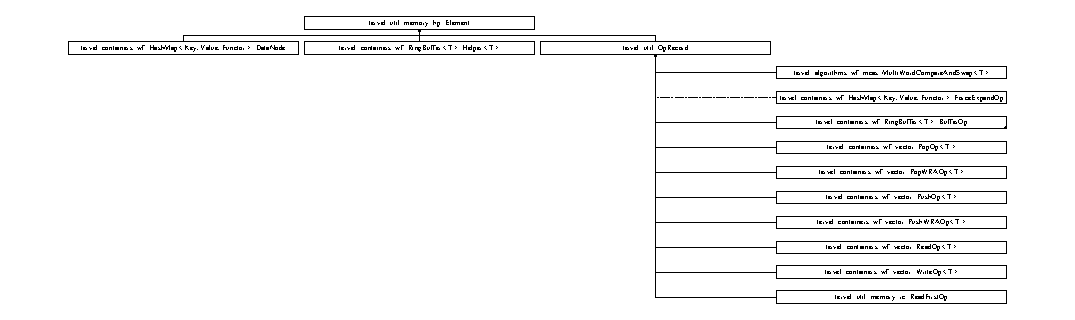
\includegraphics[height=3.853211cm]{classtervel_1_1util_1_1memory_1_1hp_1_1_element}
\end{center}
\end{figure}
\subsection*{Public Member Functions}
\begin{DoxyCompactItemize}
\item 
\hyperlink{classtervel_1_1util_1_1memory_1_1hp_1_1_element_a9b14f67c07b2bd0081978697bf7e545f}{Element} ()
\item 
virtual \hyperlink{classtervel_1_1util_1_1memory_1_1hp_1_1_element_abe65a1233e6d95b0a75c2ca3383daa86}{$\sim$\+Element} ()
\item 
void \hyperlink{classtervel_1_1util_1_1memory_1_1hp_1_1_element_af2356f697bc41aeffdc4a3e8f9aacefc}{safe\+\_\+delete} (bool no\+\_\+check=false, \hyperlink{classtervel_1_1util_1_1memory_1_1hp_1_1_element_list}{Element\+List} $\ast$const element\+\_\+list=\hyperlink{namespacetervel_a60b23602adbb2dee6160af411b74bfd3}{tervel\+::tl\+\_\+thread\+\_\+info}-\/$>$get\+\_\+hp\+\_\+element\+\_\+list())
\begin{DoxyCompactList}\small\item\em This function is used to free a hazard pointer protected object if it is safe to do so O\+R add it to a list to be freed later. \end{DoxyCompactList}\item 
virtual bool \hyperlink{classtervel_1_1util_1_1memory_1_1hp_1_1_element_a53493ef4754dd77016139863af964f90}{on\+\_\+watch} (std\+::atomic$<$ void $\ast$ $>$ $\ast$address, void $\ast$expected)
\begin{DoxyCompactList}\small\item\em This function is used to achieve a strong watch on an \hyperlink{classtervel_1_1util_1_1memory_1_1hp_1_1_element}{Element}. \end{DoxyCompactList}\item 
virtual bool \hyperlink{classtervel_1_1util_1_1memory_1_1hp_1_1_element_a88306bc6b64d0110e3ee568514dbcc04}{on\+\_\+is\+\_\+watched} ()
\begin{DoxyCompactList}\small\item\em This function is used to check a strong watch on an \hyperlink{classtervel_1_1util_1_1memory_1_1hp_1_1_element}{Element}. \end{DoxyCompactList}\item 
virtual void \hyperlink{classtervel_1_1util_1_1memory_1_1hp_1_1_element_ae71f306b6c9f08565e61546a0dc0a30c}{on\+\_\+unwatch} ()
\begin{DoxyCompactList}\small\item\em This function is used to remove a strong watch on an \hyperlink{classtervel_1_1util_1_1memory_1_1hp_1_1_element}{Element}. \end{DoxyCompactList}\end{DoxyCompactItemize}
\subsection*{Private Member Functions}
\begin{DoxyCompactItemize}
\item 
\hyperlink{classtervel_1_1util_1_1memory_1_1hp_1_1_element}{Element} $\ast$ \hyperlink{classtervel_1_1util_1_1memory_1_1hp_1_1_element_ac7b4a852a630298613bad1c57fb58d7f}{next} ()
\begin{DoxyCompactList}\small\item\em Helper method for getting the next pointer. \end{DoxyCompactList}\item 
void \hyperlink{classtervel_1_1util_1_1memory_1_1hp_1_1_element_a0611147a7c56ce225ec3129c2770eb9e}{next} (\hyperlink{classtervel_1_1util_1_1memory_1_1hp_1_1_element}{Element} $\ast$next)
\begin{DoxyCompactList}\small\item\em Helper method for setting the next pointer. \end{DoxyCompactList}\item 
\hyperlink{classtervel_1_1util_1_1memory_1_1hp_1_1_element_ad02ba6ec20e44c7a7e3cf8f9cea8e759}{D\+I\+S\+A\+L\+L\+O\+W\+\_\+\+C\+O\+P\+Y\+\_\+\+A\+N\+D\+\_\+\+A\+S\+S\+I\+G\+N} (\hyperlink{classtervel_1_1util_1_1memory_1_1hp_1_1_element}{Element})
\end{DoxyCompactItemize}
\subsection*{Private Attributes}
\begin{DoxyCompactItemize}
\item 
\hyperlink{classtervel_1_1util_1_1memory_1_1hp_1_1_element}{Element} $\ast$ \hyperlink{classtervel_1_1util_1_1memory_1_1hp_1_1_element_a6a0fa344b7f35ea4db2381a54dfd6c8d}{next\+\_\+} \{nullptr\}
\item 
friend \hyperlink{classtervel_1_1util_1_1memory_1_1hp_1_1_element_a2bede6af4da0ddbd5d5e12861432d670}{List\+Manager}
\item 
friend \hyperlink{classtervel_1_1util_1_1memory_1_1hp_1_1_element_abf4d1f696e870e12271bffb158ceb7c7}{Element\+List}
\end{DoxyCompactItemize}


\subsection{Detailed Description}
This class is used for the creation of Hazard Pointer Protected Objects Objects which extend it have the ability to call safe\+Free which delays the calling of the objects destructor until it is safe to do so. 

To achieve more advance functionality, the user can also extend \hyperlink{classtervel_1_1util_1_1_descriptor}{Descriptor} class which will provides on\+\_\+watch, on\+\_\+unwatch, and on\+\_\+is\+\_\+watch functions. 

\subsection{Constructor \& Destructor Documentation}
\hypertarget{classtervel_1_1util_1_1memory_1_1hp_1_1_element_a9b14f67c07b2bd0081978697bf7e545f}{}\index{tervel\+::util\+::memory\+::hp\+::\+Element@{tervel\+::util\+::memory\+::hp\+::\+Element}!Element@{Element}}
\index{Element@{Element}!tervel\+::util\+::memory\+::hp\+::\+Element@{tervel\+::util\+::memory\+::hp\+::\+Element}}
\subsubsection[{Element()}]{\setlength{\rightskip}{0pt plus 5cm}tervel\+::util\+::memory\+::hp\+::\+Element\+::\+Element (
\begin{DoxyParamCaption}
{}
\end{DoxyParamCaption}
)\hspace{0.3cm}{\ttfamily [inline]}}\label{classtervel_1_1util_1_1memory_1_1hp_1_1_element_a9b14f67c07b2bd0081978697bf7e545f}
\hypertarget{classtervel_1_1util_1_1memory_1_1hp_1_1_element_abe65a1233e6d95b0a75c2ca3383daa86}{}\index{tervel\+::util\+::memory\+::hp\+::\+Element@{tervel\+::util\+::memory\+::hp\+::\+Element}!````~Element@{$\sim$\+Element}}
\index{````~Element@{$\sim$\+Element}!tervel\+::util\+::memory\+::hp\+::\+Element@{tervel\+::util\+::memory\+::hp\+::\+Element}}
\subsubsection[{$\sim$\+Element()}]{\setlength{\rightskip}{0pt plus 5cm}virtual tervel\+::util\+::memory\+::hp\+::\+Element\+::$\sim$\+Element (
\begin{DoxyParamCaption}
{}
\end{DoxyParamCaption}
)\hspace{0.3cm}{\ttfamily [inline]}, {\ttfamily [virtual]}}\label{classtervel_1_1util_1_1memory_1_1hp_1_1_element_abe65a1233e6d95b0a75c2ca3383daa86}


\subsection{Member Function Documentation}
\hypertarget{classtervel_1_1util_1_1memory_1_1hp_1_1_element_ad02ba6ec20e44c7a7e3cf8f9cea8e759}{}\index{tervel\+::util\+::memory\+::hp\+::\+Element@{tervel\+::util\+::memory\+::hp\+::\+Element}!D\+I\+S\+A\+L\+L\+O\+W\+\_\+\+C\+O\+P\+Y\+\_\+\+A\+N\+D\+\_\+\+A\+S\+S\+I\+G\+N@{D\+I\+S\+A\+L\+L\+O\+W\+\_\+\+C\+O\+P\+Y\+\_\+\+A\+N\+D\+\_\+\+A\+S\+S\+I\+G\+N}}
\index{D\+I\+S\+A\+L\+L\+O\+W\+\_\+\+C\+O\+P\+Y\+\_\+\+A\+N\+D\+\_\+\+A\+S\+S\+I\+G\+N@{D\+I\+S\+A\+L\+L\+O\+W\+\_\+\+C\+O\+P\+Y\+\_\+\+A\+N\+D\+\_\+\+A\+S\+S\+I\+G\+N}!tervel\+::util\+::memory\+::hp\+::\+Element@{tervel\+::util\+::memory\+::hp\+::\+Element}}
\subsubsection[{D\+I\+S\+A\+L\+L\+O\+W\+\_\+\+C\+O\+P\+Y\+\_\+\+A\+N\+D\+\_\+\+A\+S\+S\+I\+G\+N(\+Element)}]{\setlength{\rightskip}{0pt plus 5cm}tervel\+::util\+::memory\+::hp\+::\+Element\+::\+D\+I\+S\+A\+L\+L\+O\+W\+\_\+\+C\+O\+P\+Y\+\_\+\+A\+N\+D\+\_\+\+A\+S\+S\+I\+G\+N (
\begin{DoxyParamCaption}
\item[{{\bf Element}}]{}
\end{DoxyParamCaption}
)\hspace{0.3cm}{\ttfamily [private]}}\label{classtervel_1_1util_1_1memory_1_1hp_1_1_element_ad02ba6ec20e44c7a7e3cf8f9cea8e759}
\hypertarget{classtervel_1_1util_1_1memory_1_1hp_1_1_element_ac7b4a852a630298613bad1c57fb58d7f}{}\index{tervel\+::util\+::memory\+::hp\+::\+Element@{tervel\+::util\+::memory\+::hp\+::\+Element}!next@{next}}
\index{next@{next}!tervel\+::util\+::memory\+::hp\+::\+Element@{tervel\+::util\+::memory\+::hp\+::\+Element}}
\subsubsection[{next()}]{\setlength{\rightskip}{0pt plus 5cm}{\bf Element}$\ast$ tervel\+::util\+::memory\+::hp\+::\+Element\+::next (
\begin{DoxyParamCaption}
{}
\end{DoxyParamCaption}
)\hspace{0.3cm}{\ttfamily [inline]}, {\ttfamily [private]}}\label{classtervel_1_1util_1_1memory_1_1hp_1_1_element_ac7b4a852a630298613bad1c57fb58d7f}


Helper method for getting the next pointer. 

\hypertarget{classtervel_1_1util_1_1memory_1_1hp_1_1_element_a0611147a7c56ce225ec3129c2770eb9e}{}\index{tervel\+::util\+::memory\+::hp\+::\+Element@{tervel\+::util\+::memory\+::hp\+::\+Element}!next@{next}}
\index{next@{next}!tervel\+::util\+::memory\+::hp\+::\+Element@{tervel\+::util\+::memory\+::hp\+::\+Element}}
\subsubsection[{next(\+Element $\ast$next)}]{\setlength{\rightskip}{0pt plus 5cm}void tervel\+::util\+::memory\+::hp\+::\+Element\+::next (
\begin{DoxyParamCaption}
\item[{{\bf Element} $\ast$}]{next}
\end{DoxyParamCaption}
)\hspace{0.3cm}{\ttfamily [inline]}, {\ttfamily [private]}}\label{classtervel_1_1util_1_1memory_1_1hp_1_1_element_a0611147a7c56ce225ec3129c2770eb9e}


Helper method for setting the next pointer. 

\hypertarget{classtervel_1_1util_1_1memory_1_1hp_1_1_element_a88306bc6b64d0110e3ee568514dbcc04}{}\index{tervel\+::util\+::memory\+::hp\+::\+Element@{tervel\+::util\+::memory\+::hp\+::\+Element}!on\+\_\+is\+\_\+watched@{on\+\_\+is\+\_\+watched}}
\index{on\+\_\+is\+\_\+watched@{on\+\_\+is\+\_\+watched}!tervel\+::util\+::memory\+::hp\+::\+Element@{tervel\+::util\+::memory\+::hp\+::\+Element}}
\subsubsection[{on\+\_\+is\+\_\+watched()}]{\setlength{\rightskip}{0pt plus 5cm}virtual bool tervel\+::util\+::memory\+::hp\+::\+Element\+::on\+\_\+is\+\_\+watched (
\begin{DoxyParamCaption}
{}
\end{DoxyParamCaption}
)\hspace{0.3cm}{\ttfamily [inline]}, {\ttfamily [virtual]}}\label{classtervel_1_1util_1_1memory_1_1hp_1_1_element_a88306bc6b64d0110e3ee568514dbcc04}


This function is used to check a strong watch on an \hyperlink{classtervel_1_1util_1_1memory_1_1hp_1_1_element}{Element}. 

Classes wishing to express this should override this function.

\begin{DoxyReturn}{Returns}
whether or not the element is watched. 
\end{DoxyReturn}


Reimplemented in \hyperlink{classtervel_1_1algorithms_1_1wf_1_1mcas_1_1_multi_word_compare_and_swap_aa5ee7cf4770a925939b9e7497b34473a}{tervel\+::algorithms\+::wf\+::mcas\+::\+Multi\+Word\+Compare\+And\+Swap$<$ T $>$}, and \hyperlink{classtervel_1_1util_1_1_op_record_a80c4ee47bebf246ce40bb922958dd21b}{tervel\+::util\+::\+Op\+Record}.

\hypertarget{classtervel_1_1util_1_1memory_1_1hp_1_1_element_ae71f306b6c9f08565e61546a0dc0a30c}{}\index{tervel\+::util\+::memory\+::hp\+::\+Element@{tervel\+::util\+::memory\+::hp\+::\+Element}!on\+\_\+unwatch@{on\+\_\+unwatch}}
\index{on\+\_\+unwatch@{on\+\_\+unwatch}!tervel\+::util\+::memory\+::hp\+::\+Element@{tervel\+::util\+::memory\+::hp\+::\+Element}}
\subsubsection[{on\+\_\+unwatch()}]{\setlength{\rightskip}{0pt plus 5cm}virtual void tervel\+::util\+::memory\+::hp\+::\+Element\+::on\+\_\+unwatch (
\begin{DoxyParamCaption}
{}
\end{DoxyParamCaption}
)\hspace{0.3cm}{\ttfamily [inline]}, {\ttfamily [virtual]}}\label{classtervel_1_1util_1_1memory_1_1hp_1_1_element_ae71f306b6c9f08565e61546a0dc0a30c}


This function is used to remove a strong watch on an \hyperlink{classtervel_1_1util_1_1memory_1_1hp_1_1_element}{Element}. 

Classes wishing to express this should override this function. 

Reimplemented in \hyperlink{classtervel_1_1util_1_1_op_record_a0018d1a71b9b3dcc4e2f59f34c938a46}{tervel\+::util\+::\+Op\+Record}.

\hypertarget{classtervel_1_1util_1_1memory_1_1hp_1_1_element_a53493ef4754dd77016139863af964f90}{}\index{tervel\+::util\+::memory\+::hp\+::\+Element@{tervel\+::util\+::memory\+::hp\+::\+Element}!on\+\_\+watch@{on\+\_\+watch}}
\index{on\+\_\+watch@{on\+\_\+watch}!tervel\+::util\+::memory\+::hp\+::\+Element@{tervel\+::util\+::memory\+::hp\+::\+Element}}
\subsubsection[{on\+\_\+watch(std\+::atomic$<$ void $\ast$ $>$ $\ast$address, void $\ast$expected)}]{\setlength{\rightskip}{0pt plus 5cm}virtual bool tervel\+::util\+::memory\+::hp\+::\+Element\+::on\+\_\+watch (
\begin{DoxyParamCaption}
\item[{std\+::atomic$<$ void $\ast$ $>$ $\ast$}]{address, }
\item[{void $\ast$}]{expected}
\end{DoxyParamCaption}
)\hspace{0.3cm}{\ttfamily [inline]}, {\ttfamily [virtual]}}\label{classtervel_1_1util_1_1memory_1_1hp_1_1_element_a53493ef4754dd77016139863af964f90}


This function is used to achieve a strong watch on an \hyperlink{classtervel_1_1util_1_1memory_1_1hp_1_1_element}{Element}. 

Classes wishing to express this should override this function.


\begin{DoxyParams}{Parameters}
{\em address} & the expected was load from \\
\hline
{\em expected} & the last known value of address \\
\hline
\end{DoxyParams}
\begin{DoxyReturn}{Returns}
whether or not the element was succefully watched. 
\end{DoxyReturn}


Reimplemented in \hyperlink{classtervel_1_1util_1_1_op_record_a6433f4d6d353ba6ed66e8eaefaa07d32}{tervel\+::util\+::\+Op\+Record}, and \hyperlink{classtervel_1_1containers_1_1wf_1_1_ring_buffer_1_1_helper_a2602ee377d46b4b086c5df431b851645}{tervel\+::containers\+::wf\+::\+Ring\+Buffer$<$ T $>$\+::\+Helper$<$ T $>$}.

\hypertarget{classtervel_1_1util_1_1memory_1_1hp_1_1_element_af2356f697bc41aeffdc4a3e8f9aacefc}{}\index{tervel\+::util\+::memory\+::hp\+::\+Element@{tervel\+::util\+::memory\+::hp\+::\+Element}!safe\+\_\+delete@{safe\+\_\+delete}}
\index{safe\+\_\+delete@{safe\+\_\+delete}!tervel\+::util\+::memory\+::hp\+::\+Element@{tervel\+::util\+::memory\+::hp\+::\+Element}}
\subsubsection[{safe\+\_\+delete(bool no\+\_\+check=false, Element\+List $\ast$const element\+\_\+list=tervel\+::tl\+\_\+thread\+\_\+info-\/$>$get\+\_\+hp\+\_\+element\+\_\+list())}]{\setlength{\rightskip}{0pt plus 5cm}void tervel\+::util\+::memory\+::hp\+::\+Element\+::safe\+\_\+delete (
\begin{DoxyParamCaption}
\item[{bool}]{no\+\_\+check = {\ttfamily false}, }
\item[{{\bf Element\+List} $\ast$const}]{element\+\_\+list = {\ttfamily {\bf tervel\+::tl\+\_\+thread\+\_\+info}-\/$>$get\+\_\+hp\+\_\+element\+\_\+list()}}
\end{DoxyParamCaption}
)\hspace{0.3cm}{\ttfamily [inline]}}\label{classtervel_1_1util_1_1memory_1_1hp_1_1_element_af2356f697bc41aeffdc4a3e8f9aacefc}


This function is used to free a hazard pointer protected object if it is safe to do so O\+R add it to a list to be freed later. 

It also calls \textquotesingle{}try\+\_\+to\+\_\+free\+\_\+\+Elements\textquotesingle{} in an attempt to free previously unfreeable objects.


\begin{DoxyParams}{Parameters}
{\em no\+\_\+check} & if true then the object is imeditly deleted \\
\hline
{\em element\+\_\+list} & the list to append the object to until it is safe \\
\hline
\end{DoxyParams}


\subsection{Member Data Documentation}
\hypertarget{classtervel_1_1util_1_1memory_1_1hp_1_1_element_abf4d1f696e870e12271bffb158ceb7c7}{}\index{tervel\+::util\+::memory\+::hp\+::\+Element@{tervel\+::util\+::memory\+::hp\+::\+Element}!Element\+List@{Element\+List}}
\index{Element\+List@{Element\+List}!tervel\+::util\+::memory\+::hp\+::\+Element@{tervel\+::util\+::memory\+::hp\+::\+Element}}
\subsubsection[{Element\+List}]{\setlength{\rightskip}{0pt plus 5cm}friend tervel\+::util\+::memory\+::hp\+::\+Element\+::\+Element\+List\hspace{0.3cm}{\ttfamily [private]}}\label{classtervel_1_1util_1_1memory_1_1hp_1_1_element_abf4d1f696e870e12271bffb158ceb7c7}
\hypertarget{classtervel_1_1util_1_1memory_1_1hp_1_1_element_a2bede6af4da0ddbd5d5e12861432d670}{}\index{tervel\+::util\+::memory\+::hp\+::\+Element@{tervel\+::util\+::memory\+::hp\+::\+Element}!List\+Manager@{List\+Manager}}
\index{List\+Manager@{List\+Manager}!tervel\+::util\+::memory\+::hp\+::\+Element@{tervel\+::util\+::memory\+::hp\+::\+Element}}
\subsubsection[{List\+Manager}]{\setlength{\rightskip}{0pt plus 5cm}friend tervel\+::util\+::memory\+::hp\+::\+Element\+::\+List\+Manager\hspace{0.3cm}{\ttfamily [private]}}\label{classtervel_1_1util_1_1memory_1_1hp_1_1_element_a2bede6af4da0ddbd5d5e12861432d670}
\hypertarget{classtervel_1_1util_1_1memory_1_1hp_1_1_element_a6a0fa344b7f35ea4db2381a54dfd6c8d}{}\index{tervel\+::util\+::memory\+::hp\+::\+Element@{tervel\+::util\+::memory\+::hp\+::\+Element}!next\+\_\+@{next\+\_\+}}
\index{next\+\_\+@{next\+\_\+}!tervel\+::util\+::memory\+::hp\+::\+Element@{tervel\+::util\+::memory\+::hp\+::\+Element}}
\subsubsection[{next\+\_\+}]{\setlength{\rightskip}{0pt plus 5cm}{\bf Element}$\ast$ tervel\+::util\+::memory\+::hp\+::\+Element\+::next\+\_\+ \{nullptr\}\hspace{0.3cm}{\ttfamily [private]}}\label{classtervel_1_1util_1_1memory_1_1hp_1_1_element_a6a0fa344b7f35ea4db2381a54dfd6c8d}


The documentation for this class was generated from the following file\+:\begin{DoxyCompactItemize}
\item 
tervel/util/memory/hp/\hyperlink{hp__element_8h}{hp\+\_\+element.\+h}\end{DoxyCompactItemize}

\hypertarget{classtervel_1_1util_1_1memory_1_1hp_1_1_element_list}{}\section{tervel\+:\+:util\+:\+:memory\+:\+:hp\+:\+:Element\+List Class Reference}
\label{classtervel_1_1util_1_1memory_1_1hp_1_1_element_list}\index{tervel\+::util\+::memory\+::hp\+::\+Element\+List@{tervel\+::util\+::memory\+::hp\+::\+Element\+List}}


Defines a list of objects which are stored until they are safe to be freed.  




{\ttfamily \#include $<$hp\+\_\+list.\+h$>$}

\subsection*{Public Member Functions}
\begin{DoxyCompactItemize}
\item 
\hyperlink{classtervel_1_1util_1_1memory_1_1hp_1_1_element_list_a08f1ad218521948919aa8232098d69fb}{Element\+List} (\hyperlink{classtervel_1_1util_1_1memory_1_1hp_1_1_list_manager}{List\+Manager} $\ast$manager)
\item 
\hyperlink{classtervel_1_1util_1_1memory_1_1hp_1_1_element_list_a4ca58faad54530a724b61dfc5dc2f73b}{$\sim$\+Element\+List} ()
\end{DoxyCompactItemize}
\subsection*{Public Attributes}
\begin{DoxyCompactItemize}
\item 
friend \hyperlink{classtervel_1_1util_1_1memory_1_1hp_1_1_element_list_a2392e8dcf3dc26d7766c92a875696649}{Element}
\end{DoxyCompactItemize}
\subsection*{Private Member Functions}
\begin{DoxyCompactItemize}
\item 
void \hyperlink{classtervel_1_1util_1_1memory_1_1hp_1_1_element_list_adf7724a6cc985cde89f6195bbfd9d656}{send\+\_\+to\+\_\+manager} ()
\begin{DoxyCompactList}\small\item\em Sends all elements managed by this list to the parent. \end{DoxyCompactList}\item 
void \hyperlink{classtervel_1_1util_1_1memory_1_1hp_1_1_element_list_a694cee8f0e74e14e9af680f48f28b109}{add\+\_\+to\+\_\+unsafe} (\hyperlink{classtervel_1_1util_1_1memory_1_1hp_1_1_element}{Element} $\ast$elem)
\begin{DoxyCompactList}\small\item\em This function adds an \hyperlink{classtervel_1_1util_1_1memory_1_1hp_1_1_element}{Element} to the unsafe list. \end{DoxyCompactList}\item 
void \hyperlink{classtervel_1_1util_1_1memory_1_1hp_1_1_element_list_a595805e2257bf2f276ad2e0ecf8dd675}{try\+\_\+to\+\_\+free\+\_\+elements} (bool dont\+\_\+check=false)
\begin{DoxyCompactList}\small\item\em Tries to free elements from the unsafe list. \end{DoxyCompactList}\end{DoxyCompactItemize}
\subsection*{Private Attributes}
\begin{DoxyCompactItemize}
\item 
\hyperlink{classtervel_1_1util_1_1memory_1_1hp_1_1_list_manager}{List\+Manager} $\ast$ \hyperlink{classtervel_1_1util_1_1memory_1_1hp_1_1_element_list_a59a6505303f5914110a624570b5c902d}{manager\+\_\+}
\begin{DoxyCompactList}\small\item\em This list\textquotesingle{}s manager. \end{DoxyCompactList}\item 
\hyperlink{classtervel_1_1util_1_1memory_1_1hp_1_1_element}{Element} $\ast$ \hyperlink{classtervel_1_1util_1_1memory_1_1hp_1_1_element_list_a7522322f344cde24db1524ce4e4666d1}{element\+\_\+list\+\_\+} \{nullptr\}
\begin{DoxyCompactList}\small\item\em A linked list of list elements. \end{DoxyCompactList}\end{DoxyCompactItemize}


\subsection{Detailed Description}
Defines a list of objects which are stored until they are safe to be freed. 

The list is represented as a linked list of H\+P Elements

Further, this object has a parent who is shared amongst other threads. When it is to be destroyed, it sends its remaining elements to the parent, relinquishing ownership of said elements. 

\subsection{Constructor \& Destructor Documentation}
\hypertarget{classtervel_1_1util_1_1memory_1_1hp_1_1_element_list_a08f1ad218521948919aa8232098d69fb}{}\index{tervel\+::util\+::memory\+::hp\+::\+Element\+List@{tervel\+::util\+::memory\+::hp\+::\+Element\+List}!Element\+List@{Element\+List}}
\index{Element\+List@{Element\+List}!tervel\+::util\+::memory\+::hp\+::\+Element\+List@{tervel\+::util\+::memory\+::hp\+::\+Element\+List}}
\subsubsection[{Element\+List(\+List\+Manager $\ast$manager)}]{\setlength{\rightskip}{0pt plus 5cm}tervel\+::util\+::memory\+::hp\+::\+Element\+List\+::\+Element\+List (
\begin{DoxyParamCaption}
\item[{{\bf List\+Manager} $\ast$}]{manager}
\end{DoxyParamCaption}
)\hspace{0.3cm}{\ttfamily [inline]}, {\ttfamily [explicit]}}\label{classtervel_1_1util_1_1memory_1_1hp_1_1_element_list_a08f1ad218521948919aa8232098d69fb}
\hypertarget{classtervel_1_1util_1_1memory_1_1hp_1_1_element_list_a4ca58faad54530a724b61dfc5dc2f73b}{}\index{tervel\+::util\+::memory\+::hp\+::\+Element\+List@{tervel\+::util\+::memory\+::hp\+::\+Element\+List}!````~Element\+List@{$\sim$\+Element\+List}}
\index{````~Element\+List@{$\sim$\+Element\+List}!tervel\+::util\+::memory\+::hp\+::\+Element\+List@{tervel\+::util\+::memory\+::hp\+::\+Element\+List}}
\subsubsection[{$\sim$\+Element\+List()}]{\setlength{\rightskip}{0pt plus 5cm}tervel\+::util\+::memory\+::hp\+::\+Element\+List\+::$\sim$\+Element\+List (
\begin{DoxyParamCaption}
{}
\end{DoxyParamCaption}
)\hspace{0.3cm}{\ttfamily [inline]}}\label{classtervel_1_1util_1_1memory_1_1hp_1_1_element_list_a4ca58faad54530a724b61dfc5dc2f73b}


\subsection{Member Function Documentation}
\hypertarget{classtervel_1_1util_1_1memory_1_1hp_1_1_element_list_a694cee8f0e74e14e9af680f48f28b109}{}\index{tervel\+::util\+::memory\+::hp\+::\+Element\+List@{tervel\+::util\+::memory\+::hp\+::\+Element\+List}!add\+\_\+to\+\_\+unsafe@{add\+\_\+to\+\_\+unsafe}}
\index{add\+\_\+to\+\_\+unsafe@{add\+\_\+to\+\_\+unsafe}!tervel\+::util\+::memory\+::hp\+::\+Element\+List@{tervel\+::util\+::memory\+::hp\+::\+Element\+List}}
\subsubsection[{add\+\_\+to\+\_\+unsafe(\+Element $\ast$elem)}]{\setlength{\rightskip}{0pt plus 5cm}void tervel\+::util\+::memory\+::hp\+::\+Element\+List\+::add\+\_\+to\+\_\+unsafe (
\begin{DoxyParamCaption}
\item[{{\bf Element} $\ast$}]{elem}
\end{DoxyParamCaption}
)\hspace{0.3cm}{\ttfamily [private]}}\label{classtervel_1_1util_1_1memory_1_1hp_1_1_element_list_a694cee8f0e74e14e9af680f48f28b109}


This function adds an \hyperlink{classtervel_1_1util_1_1memory_1_1hp_1_1_element}{Element} to the unsafe list. 


\begin{DoxyParams}{Parameters}
{\em elem} & The element to add \\
\hline
\end{DoxyParams}
\hypertarget{classtervel_1_1util_1_1memory_1_1hp_1_1_element_list_adf7724a6cc985cde89f6195bbfd9d656}{}\index{tervel\+::util\+::memory\+::hp\+::\+Element\+List@{tervel\+::util\+::memory\+::hp\+::\+Element\+List}!send\+\_\+to\+\_\+manager@{send\+\_\+to\+\_\+manager}}
\index{send\+\_\+to\+\_\+manager@{send\+\_\+to\+\_\+manager}!tervel\+::util\+::memory\+::hp\+::\+Element\+List@{tervel\+::util\+::memory\+::hp\+::\+Element\+List}}
\subsubsection[{send\+\_\+to\+\_\+manager()}]{\setlength{\rightskip}{0pt plus 5cm}void tervel\+::util\+::memory\+::hp\+::\+Element\+List\+::send\+\_\+to\+\_\+manager (
\begin{DoxyParamCaption}
{}
\end{DoxyParamCaption}
)\hspace{0.3cm}{\ttfamily [private]}}\label{classtervel_1_1util_1_1memory_1_1hp_1_1_element_list_adf7724a6cc985cde89f6195bbfd9d656}


Sends all elements managed by this list to the parent. 

\hypertarget{classtervel_1_1util_1_1memory_1_1hp_1_1_element_list_a595805e2257bf2f276ad2e0ecf8dd675}{}\index{tervel\+::util\+::memory\+::hp\+::\+Element\+List@{tervel\+::util\+::memory\+::hp\+::\+Element\+List}!try\+\_\+to\+\_\+free\+\_\+elements@{try\+\_\+to\+\_\+free\+\_\+elements}}
\index{try\+\_\+to\+\_\+free\+\_\+elements@{try\+\_\+to\+\_\+free\+\_\+elements}!tervel\+::util\+::memory\+::hp\+::\+Element\+List@{tervel\+::util\+::memory\+::hp\+::\+Element\+List}}
\subsubsection[{try\+\_\+to\+\_\+free\+\_\+elements(bool dont\+\_\+check=false)}]{\setlength{\rightskip}{0pt plus 5cm}void tervel\+::util\+::memory\+::hp\+::\+Element\+List\+::try\+\_\+to\+\_\+free\+\_\+elements (
\begin{DoxyParamCaption}
\item[{bool}]{dont\+\_\+check = {\ttfamily false}}
\end{DoxyParamCaption}
)\hspace{0.3cm}{\ttfamily [private]}}\label{classtervel_1_1util_1_1memory_1_1hp_1_1_element_list_a595805e2257bf2f276ad2e0ecf8dd675}


Tries to free elements from the unsafe list. 


\begin{DoxyParams}{Parameters}
{\em dont\+\_\+check} & If true, it ignores safety checks \\
\hline
\end{DoxyParams}


\subsection{Member Data Documentation}
\hypertarget{classtervel_1_1util_1_1memory_1_1hp_1_1_element_list_a2392e8dcf3dc26d7766c92a875696649}{}\index{tervel\+::util\+::memory\+::hp\+::\+Element\+List@{tervel\+::util\+::memory\+::hp\+::\+Element\+List}!Element@{Element}}
\index{Element@{Element}!tervel\+::util\+::memory\+::hp\+::\+Element\+List@{tervel\+::util\+::memory\+::hp\+::\+Element\+List}}
\subsubsection[{Element}]{\setlength{\rightskip}{0pt plus 5cm}friend tervel\+::util\+::memory\+::hp\+::\+Element\+List\+::\+Element}\label{classtervel_1_1util_1_1memory_1_1hp_1_1_element_list_a2392e8dcf3dc26d7766c92a875696649}
\hypertarget{classtervel_1_1util_1_1memory_1_1hp_1_1_element_list_a7522322f344cde24db1524ce4e4666d1}{}\index{tervel\+::util\+::memory\+::hp\+::\+Element\+List@{tervel\+::util\+::memory\+::hp\+::\+Element\+List}!element\+\_\+list\+\_\+@{element\+\_\+list\+\_\+}}
\index{element\+\_\+list\+\_\+@{element\+\_\+list\+\_\+}!tervel\+::util\+::memory\+::hp\+::\+Element\+List@{tervel\+::util\+::memory\+::hp\+::\+Element\+List}}
\subsubsection[{element\+\_\+list\+\_\+}]{\setlength{\rightskip}{0pt plus 5cm}{\bf Element}$\ast$ tervel\+::util\+::memory\+::hp\+::\+Element\+List\+::element\+\_\+list\+\_\+ \{nullptr\}\hspace{0.3cm}{\ttfamily [private]}}\label{classtervel_1_1util_1_1memory_1_1hp_1_1_element_list_a7522322f344cde24db1524ce4e4666d1}


A linked list of list elements. 

Elements are freed when they are no longer referenced by other threads. \hypertarget{classtervel_1_1util_1_1memory_1_1hp_1_1_element_list_a59a6505303f5914110a624570b5c902d}{}\index{tervel\+::util\+::memory\+::hp\+::\+Element\+List@{tervel\+::util\+::memory\+::hp\+::\+Element\+List}!manager\+\_\+@{manager\+\_\+}}
\index{manager\+\_\+@{manager\+\_\+}!tervel\+::util\+::memory\+::hp\+::\+Element\+List@{tervel\+::util\+::memory\+::hp\+::\+Element\+List}}
\subsubsection[{manager\+\_\+}]{\setlength{\rightskip}{0pt plus 5cm}{\bf List\+Manager}$\ast$ tervel\+::util\+::memory\+::hp\+::\+Element\+List\+::manager\+\_\+\hspace{0.3cm}{\ttfamily [private]}}\label{classtervel_1_1util_1_1memory_1_1hp_1_1_element_list_a59a6505303f5914110a624570b5c902d}


This list\textquotesingle{}s manager. 



The documentation for this class was generated from the following file\+:\begin{DoxyCompactItemize}
\item 
tervel/util/memory/hp/\hyperlink{hp__list_8h}{hp\+\_\+list.\+h}\end{DoxyCompactItemize}

\hypertarget{classtervel_1_1containers_1_1wf_1_1_ring_buffer_1_1_enqueue_op}{}\section{tervel\+:\+:containers\+:\+:wf\+:\+:Ring\+Buffer$<$ T $>$\+:\+:Enqueue\+Op$<$ T $>$ Class Template Reference}
\label{classtervel_1_1containers_1_1wf_1_1_ring_buffer_1_1_enqueue_op}\index{tervel\+::containers\+::wf\+::\+Ring\+Buffer$<$ T $>$\+::\+Enqueue\+Op$<$ T $>$@{tervel\+::containers\+::wf\+::\+Ring\+Buffer$<$ T $>$\+::\+Enqueue\+Op$<$ T $>$}}


{\ttfamily \#include $<$enqueue\+\_\+op.\+h$>$}

Inheritance diagram for tervel\+:\+:containers\+:\+:wf\+:\+:Ring\+Buffer$<$ T $>$\+:\+:Enqueue\+Op$<$ T $>$\+:\begin{figure}[H]
\begin{center}
\leavevmode
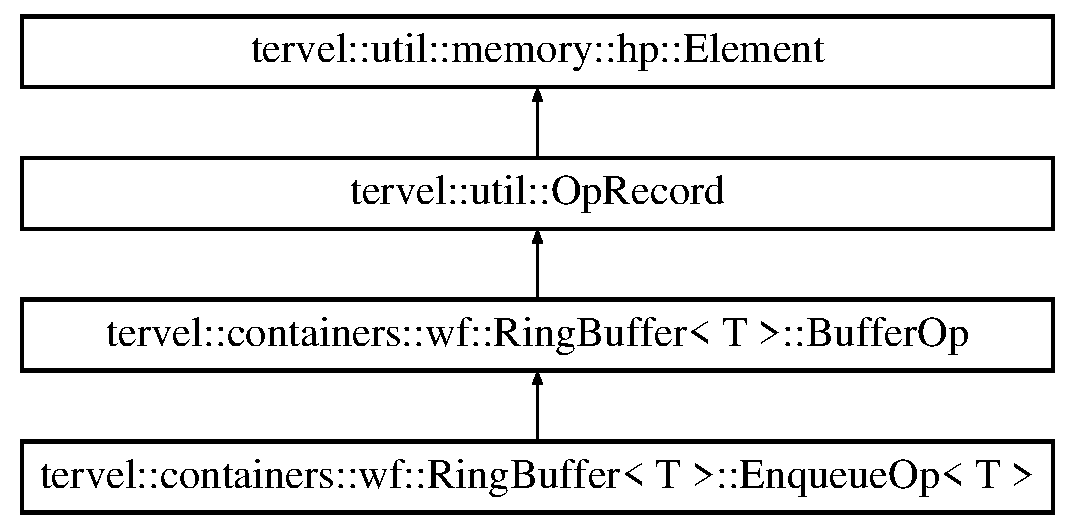
\includegraphics[height=4.000000cm]{classtervel_1_1containers_1_1wf_1_1_ring_buffer_1_1_enqueue_op}
\end{center}
\end{figure}
\subsection*{Public Member Functions}
\begin{DoxyCompactItemize}
\item 
\hyperlink{classtervel_1_1containers_1_1wf_1_1_ring_buffer_1_1_enqueue_op_ac3525c0a93c6f9c479b3631645fb6f49}{Enqueue\+Op} (\hyperlink{classtervel_1_1containers_1_1wf_1_1_ring_buffer}{Ring\+Buffer}$<$ T $>$ $\ast$rb, T value)
\item 
void $\ast$ \hyperlink{classtervel_1_1containers_1_1wf_1_1_ring_buffer_1_1_enqueue_op_a746cece514a2d8189bad01c04a1cf00c}{associate} (\hyperlink{classtervel_1_1containers_1_1wf_1_1_ring_buffer_1_1_helper}{Helper} $\ast$h)
\item 
void \hyperlink{classtervel_1_1containers_1_1wf_1_1_ring_buffer_1_1_enqueue_op_a928f562593a93be6c99df05c128012b8}{help\+\_\+complete} ()
\begin{DoxyCompactList}\small\item\em Implementations of this function that upon its return the operation described in the Op\+Record has been completed. \end{DoxyCompactList}\item 
bool \hyperlink{classtervel_1_1containers_1_1wf_1_1_ring_buffer_1_1_enqueue_op_abb16cd7e84e8d3d1ffe1f25a400ac36c}{result} ()
\end{DoxyCompactItemize}
\subsection*{Private Member Functions}
\begin{DoxyCompactItemize}
\item 
\hyperlink{classtervel_1_1containers_1_1wf_1_1_ring_buffer_1_1_enqueue_op_ada0000413005d66f893690c9bb9255e4}{D\+I\+S\+A\+L\+L\+O\+W\+\_\+\+C\+O\+P\+Y\+\_\+\+A\+N\+D\+\_\+\+A\+S\+S\+I\+G\+N} (\hyperlink{classtervel_1_1containers_1_1wf_1_1_ring_buffer_1_1_enqueue_op}{Enqueue\+Op})
\end{DoxyCompactItemize}
\subsection*{Private Attributes}
\begin{DoxyCompactItemize}
\item 
const T \hyperlink{classtervel_1_1containers_1_1wf_1_1_ring_buffer_1_1_enqueue_op_a860df72b95b0dca2d419fb0b65361982}{value\+\_\+}
\end{DoxyCompactItemize}
\subsection*{Additional Inherited Members}


\subsection{Constructor \& Destructor Documentation}
\hypertarget{classtervel_1_1containers_1_1wf_1_1_ring_buffer_1_1_enqueue_op_ac3525c0a93c6f9c479b3631645fb6f49}{}\index{tervel\+::containers\+::wf\+::\+Ring\+Buffer\+::\+Enqueue\+Op@{tervel\+::containers\+::wf\+::\+Ring\+Buffer\+::\+Enqueue\+Op}!Enqueue\+Op@{Enqueue\+Op}}
\index{Enqueue\+Op@{Enqueue\+Op}!tervel\+::containers\+::wf\+::\+Ring\+Buffer\+::\+Enqueue\+Op@{tervel\+::containers\+::wf\+::\+Ring\+Buffer\+::\+Enqueue\+Op}}
\subsubsection[{Enqueue\+Op(\+Ring\+Buffer$<$ T $>$ $\ast$rb, T value)}]{\setlength{\rightskip}{0pt plus 5cm}template$<$typename T$>$ template$<$typename T $>$ {\bf tervel\+::containers\+::wf\+::\+Ring\+Buffer}$<$ T $>$\+::{\bf Enqueue\+Op}$<$ T $>$\+::{\bf Enqueue\+Op} (
\begin{DoxyParamCaption}
\item[{{\bf Ring\+Buffer}$<$ T $>$ $\ast$}]{rb, }
\item[{T}]{value}
\end{DoxyParamCaption}
)\hspace{0.3cm}{\ttfamily [inline]}}\label{classtervel_1_1containers_1_1wf_1_1_ring_buffer_1_1_enqueue_op_ac3525c0a93c6f9c479b3631645fb6f49}


\subsection{Member Function Documentation}
\hypertarget{classtervel_1_1containers_1_1wf_1_1_ring_buffer_1_1_enqueue_op_a746cece514a2d8189bad01c04a1cf00c}{}\index{tervel\+::containers\+::wf\+::\+Ring\+Buffer\+::\+Enqueue\+Op@{tervel\+::containers\+::wf\+::\+Ring\+Buffer\+::\+Enqueue\+Op}!associate@{associate}}
\index{associate@{associate}!tervel\+::containers\+::wf\+::\+Ring\+Buffer\+::\+Enqueue\+Op@{tervel\+::containers\+::wf\+::\+Ring\+Buffer\+::\+Enqueue\+Op}}
\subsubsection[{associate(\+Helper $\ast$h)}]{\setlength{\rightskip}{0pt plus 5cm}template$<$typename T$>$ template$<$typename T $>$ void $\ast$ {\bf tervel\+::containers\+::wf\+::\+Ring\+Buffer}$<$ T $>$\+::{\bf Enqueue\+Op}$<$ T $>$\+::associate (
\begin{DoxyParamCaption}
\item[{{\bf Helper} $\ast$}]{h}
\end{DoxyParamCaption}
)\hspace{0.3cm}{\ttfamily [virtual]}}\label{classtervel_1_1containers_1_1wf_1_1_ring_buffer_1_1_enqueue_op_a746cece514a2d8189bad01c04a1cf00c}


Implements \hyperlink{classtervel_1_1containers_1_1wf_1_1_ring_buffer_1_1_buffer_op_a345d7432fa98f44f1620f5f718ff7a1e}{tervel\+::containers\+::wf\+::\+Ring\+Buffer$<$ T $>$\+::\+Buffer\+Op}.

\hypertarget{classtervel_1_1containers_1_1wf_1_1_ring_buffer_1_1_enqueue_op_ada0000413005d66f893690c9bb9255e4}{}\index{tervel\+::containers\+::wf\+::\+Ring\+Buffer\+::\+Enqueue\+Op@{tervel\+::containers\+::wf\+::\+Ring\+Buffer\+::\+Enqueue\+Op}!D\+I\+S\+A\+L\+L\+O\+W\+\_\+\+C\+O\+P\+Y\+\_\+\+A\+N\+D\+\_\+\+A\+S\+S\+I\+G\+N@{D\+I\+S\+A\+L\+L\+O\+W\+\_\+\+C\+O\+P\+Y\+\_\+\+A\+N\+D\+\_\+\+A\+S\+S\+I\+G\+N}}
\index{D\+I\+S\+A\+L\+L\+O\+W\+\_\+\+C\+O\+P\+Y\+\_\+\+A\+N\+D\+\_\+\+A\+S\+S\+I\+G\+N@{D\+I\+S\+A\+L\+L\+O\+W\+\_\+\+C\+O\+P\+Y\+\_\+\+A\+N\+D\+\_\+\+A\+S\+S\+I\+G\+N}!tervel\+::containers\+::wf\+::\+Ring\+Buffer\+::\+Enqueue\+Op@{tervel\+::containers\+::wf\+::\+Ring\+Buffer\+::\+Enqueue\+Op}}
\subsubsection[{D\+I\+S\+A\+L\+L\+O\+W\+\_\+\+C\+O\+P\+Y\+\_\+\+A\+N\+D\+\_\+\+A\+S\+S\+I\+G\+N(\+Enqueue\+Op)}]{\setlength{\rightskip}{0pt plus 5cm}template$<$typename T$>$ template$<$typename T $>$ {\bf tervel\+::containers\+::wf\+::\+Ring\+Buffer}$<$ T $>$\+::{\bf Enqueue\+Op}$<$ T $>$\+::D\+I\+S\+A\+L\+L\+O\+W\+\_\+\+C\+O\+P\+Y\+\_\+\+A\+N\+D\+\_\+\+A\+S\+S\+I\+G\+N (
\begin{DoxyParamCaption}
\item[{{\bf Enqueue\+Op}$<$ T $>$}]{}
\end{DoxyParamCaption}
)\hspace{0.3cm}{\ttfamily [private]}}\label{classtervel_1_1containers_1_1wf_1_1_ring_buffer_1_1_enqueue_op_ada0000413005d66f893690c9bb9255e4}
\hypertarget{classtervel_1_1containers_1_1wf_1_1_ring_buffer_1_1_enqueue_op_a928f562593a93be6c99df05c128012b8}{}\index{tervel\+::containers\+::wf\+::\+Ring\+Buffer\+::\+Enqueue\+Op@{tervel\+::containers\+::wf\+::\+Ring\+Buffer\+::\+Enqueue\+Op}!help\+\_\+complete@{help\+\_\+complete}}
\index{help\+\_\+complete@{help\+\_\+complete}!tervel\+::containers\+::wf\+::\+Ring\+Buffer\+::\+Enqueue\+Op@{tervel\+::containers\+::wf\+::\+Ring\+Buffer\+::\+Enqueue\+Op}}
\subsubsection[{help\+\_\+complete()}]{\setlength{\rightskip}{0pt plus 5cm}template$<$typename T$>$ template$<$typename T $>$ void {\bf tervel\+::containers\+::wf\+::\+Ring\+Buffer}$<$ T $>$\+::{\bf Enqueue\+Op}$<$ T $>$\+::help\+\_\+complete (
\begin{DoxyParamCaption}
{}
\end{DoxyParamCaption}
)\hspace{0.3cm}{\ttfamily [virtual]}}\label{classtervel_1_1containers_1_1wf_1_1_ring_buffer_1_1_enqueue_op_a928f562593a93be6c99df05c128012b8}


Implementations of this function that upon its return the operation described in the Op\+Record has been completed. 

As such it must be thread-\/safe and the extending class must contain all the information necessary to complete the operation. 

Implements \hyperlink{classtervel_1_1util_1_1_op_record_aa75ab39688a8d4cceb6a1ef0409537c0}{tervel\+::util\+::\+Op\+Record}.

\hypertarget{classtervel_1_1containers_1_1wf_1_1_ring_buffer_1_1_enqueue_op_abb16cd7e84e8d3d1ffe1f25a400ac36c}{}\index{tervel\+::containers\+::wf\+::\+Ring\+Buffer\+::\+Enqueue\+Op@{tervel\+::containers\+::wf\+::\+Ring\+Buffer\+::\+Enqueue\+Op}!result@{result}}
\index{result@{result}!tervel\+::containers\+::wf\+::\+Ring\+Buffer\+::\+Enqueue\+Op@{tervel\+::containers\+::wf\+::\+Ring\+Buffer\+::\+Enqueue\+Op}}
\subsubsection[{result()}]{\setlength{\rightskip}{0pt plus 5cm}template$<$typename T$>$ template$<$typename T $>$ bool {\bf tervel\+::containers\+::wf\+::\+Ring\+Buffer}$<$ T $>$\+::{\bf Enqueue\+Op}$<$ T $>$\+::result (
\begin{DoxyParamCaption}
{}
\end{DoxyParamCaption}
)}\label{classtervel_1_1containers_1_1wf_1_1_ring_buffer_1_1_enqueue_op_abb16cd7e84e8d3d1ffe1f25a400ac36c}


\subsection{Member Data Documentation}
\hypertarget{classtervel_1_1containers_1_1wf_1_1_ring_buffer_1_1_enqueue_op_a860df72b95b0dca2d419fb0b65361982}{}\index{tervel\+::containers\+::wf\+::\+Ring\+Buffer\+::\+Enqueue\+Op@{tervel\+::containers\+::wf\+::\+Ring\+Buffer\+::\+Enqueue\+Op}!value\+\_\+@{value\+\_\+}}
\index{value\+\_\+@{value\+\_\+}!tervel\+::containers\+::wf\+::\+Ring\+Buffer\+::\+Enqueue\+Op@{tervel\+::containers\+::wf\+::\+Ring\+Buffer\+::\+Enqueue\+Op}}
\subsubsection[{value\+\_\+}]{\setlength{\rightskip}{0pt plus 5cm}template$<$typename T$>$ template$<$typename T $>$ const T {\bf tervel\+::containers\+::wf\+::\+Ring\+Buffer}$<$ T $>$\+::{\bf Enqueue\+Op}$<$ T $>$\+::value\+\_\+\hspace{0.3cm}{\ttfamily [private]}}\label{classtervel_1_1containers_1_1wf_1_1_ring_buffer_1_1_enqueue_op_a860df72b95b0dca2d419fb0b65361982}


The documentation for this class was generated from the following files\+:\begin{DoxyCompactItemize}
\item 
tervel/containers/wf/ring-\/buffer/\hyperlink{enqueue__op_8h}{enqueue\+\_\+op.\+h}\item 
tervel/containers/wf/ring-\/buffer/\hyperlink{enqueue__op__imp_8h}{enqueue\+\_\+op\+\_\+imp.\+h}\end{DoxyCompactItemize}

\hypertarget{struct_test_class_1_1equal__to}{}\section{Test\+Class$<$ Key, Value $>$\+:\+:equal\+\_\+to$<$ T $>$ Struct Template Reference}
\label{struct_test_class_1_1equal__to}\index{Test\+Class$<$ Key, Value $>$\+::equal\+\_\+to$<$ T $>$@{Test\+Class$<$ Key, Value $>$\+::equal\+\_\+to$<$ T $>$}}
Inheritance diagram for Test\+Class$<$ Key, Value $>$\+:\+:equal\+\_\+to$<$ T $>$\+:\begin{figure}[H]
\begin{center}
\leavevmode
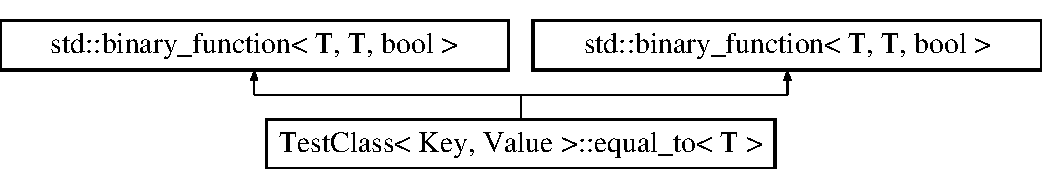
\includegraphics[height=2.000000cm]{struct_test_class_1_1equal__to}
\end{center}
\end{figure}
\subsection*{Public Member Functions}
\begin{DoxyCompactItemize}
\item 
bool \hyperlink{struct_test_class_1_1equal__to_afb3bfd12cfd80edd94463b71702c8718}{operator()} (const T \&x, const T \&y) const 
\item 
bool \hyperlink{struct_test_class_1_1equal__to_afb3bfd12cfd80edd94463b71702c8718}{operator()} (const T \&x, const T \&y) const 
\end{DoxyCompactItemize}


\subsection{Member Function Documentation}
\hypertarget{struct_test_class_1_1equal__to_afb3bfd12cfd80edd94463b71702c8718}{}\index{Test\+Class\+::equal\+\_\+to@{Test\+Class\+::equal\+\_\+to}!operator()@{operator()}}
\index{operator()@{operator()}!Test\+Class\+::equal\+\_\+to@{Test\+Class\+::equal\+\_\+to}}
\subsubsection[{operator()(const T \&x, const T \&y) const }]{\setlength{\rightskip}{0pt plus 5cm}template$<$class Key, class Value$>$ template$<$class T $>$ bool {\bf Test\+Class}$<$ Key, {\bf Value} $>$\+::{\bf equal\+\_\+to}$<$ T $>$\+::operator() (
\begin{DoxyParamCaption}
\item[{const T \&}]{x, }
\item[{const T \&}]{y}
\end{DoxyParamCaption}
) const\hspace{0.3cm}{\ttfamily [inline]}}\label{struct_test_class_1_1equal__to_afb3bfd12cfd80edd94463b71702c8718}
\hypertarget{struct_test_class_1_1equal__to_afb3bfd12cfd80edd94463b71702c8718}{}\index{Test\+Class\+::equal\+\_\+to@{Test\+Class\+::equal\+\_\+to}!operator()@{operator()}}
\index{operator()@{operator()}!Test\+Class\+::equal\+\_\+to@{Test\+Class\+::equal\+\_\+to}}
\subsubsection[{operator()(const T \&x, const T \&y) const }]{\setlength{\rightskip}{0pt plus 5cm}template$<$class Key, class Value$>$ template$<$class T $>$ bool {\bf Test\+Class}$<$ Key, {\bf Value} $>$\+::{\bf equal\+\_\+to}$<$ T $>$\+::operator() (
\begin{DoxyParamCaption}
\item[{const T \&}]{x, }
\item[{const T \&}]{y}
\end{DoxyParamCaption}
) const\hspace{0.3cm}{\ttfamily [inline]}}\label{struct_test_class_1_1equal__to_afb3bfd12cfd80edd94463b71702c8718}


The documentation for this struct was generated from the following files\+:\begin{DoxyCompactItemize}
\item 
tervel/tests/hash\+\_\+map/api/\hyperlink{lock__boost__map_8h}{lock\+\_\+boost\+\_\+map.\+h}\item 
tervel/tests/hash\+\_\+map/api/\hyperlink{lock__stl__map_8h}{lock\+\_\+stl\+\_\+map.\+h}\end{DoxyCompactItemize}

\hypertarget{class_erase_at}{}\section{Erase\+At$<$ T $>$ Class Template Reference}
\label{class_erase_at}\index{Erase\+At$<$ T $>$@{Erase\+At$<$ T $>$}}


{\ttfamily \#include $<$earaseat\+\_\+op.\+h$>$}

Inheritance diagram for Erase\+At$<$ T $>$\+:\begin{figure}[H]
\begin{center}
\leavevmode
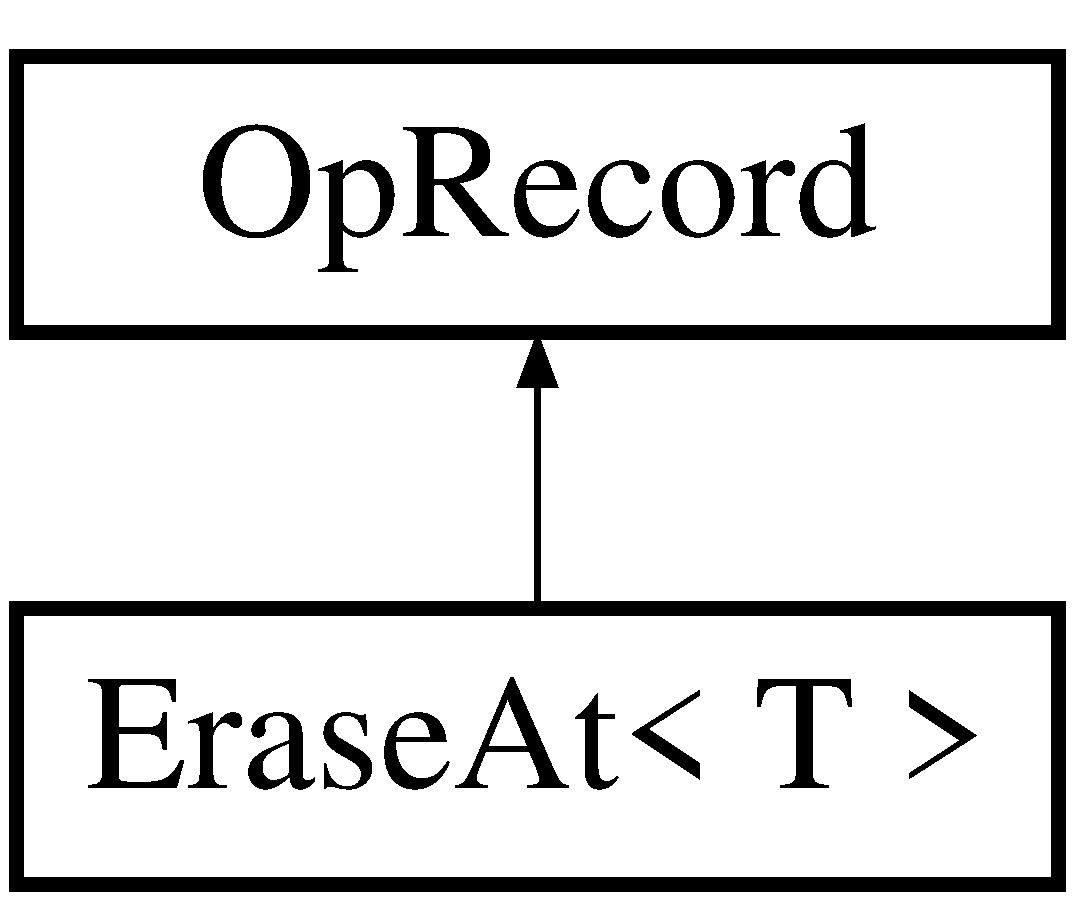
\includegraphics[height=2.000000cm]{class_erase_at}
\end{center}
\end{figure}
\subsection*{Public Member Functions}
\begin{DoxyCompactItemize}
\item 
\hyperlink{class_erase_at_a4f96bd2292727d90cecbaac7aa356aeb}{Erase\+At} (const Vector $\ast$vector, const size\+\_\+t idx)
\item 
bool \hyperlink{class_erase_at_a8db28ef12f418e3e7bc745fb32038b78}{begin} (const T \&result)
\item 
void \hyperlink{class_erase_at_ac69fc35afacc8da116cf093f100fff69}{execute} ()
\item 
void \hyperlink{class_erase_at_a47c62ba991eb506ffe67a73e0317673d}{cleanup} ()
\item 
bool \hyperlink{class_erase_at_ae8f9925c82a249f5467da3036747d340}{complete} (int pos)
\item 
bool \hyperlink{class_erase_at_a6f6a5c68a1bae7683b10f403702f0f88}{is\+\_\+complete} ()
\end{DoxyCompactItemize}
\subsection*{Public Attributes}
\begin{DoxyCompactItemize}
\item 
const size\+\_\+t \hyperlink{class_erase_at_ab067b4f8d097677748b1cd081730e450}{idx\+\_\+}
\item 
const Vector$<$ T $>$ $\ast$ \hyperlink{class_erase_at_a7a24a5872cd3fa48cb71711b96e15af9}{vector\+\_\+}
\item 
std\+::atomic$<$ bool $>$ \hyperlink{class_erase_at_a7a0e20cf5a5e02822dd1d0a3d486920c}{is\+\_\+complete\+\_\+}
\item 
std\+::atomic$<$ helper\+\_\+t $\ast$ $>$ \hyperlink{class_erase_at_a6fe6f561569a440fa9f8631d6c06d895}{next\+\_\+}
\end{DoxyCompactItemize}


\subsection{Constructor \& Destructor Documentation}
\hypertarget{class_erase_at_a4f96bd2292727d90cecbaac7aa356aeb}{}\index{Erase\+At@{Erase\+At}!Erase\+At@{Erase\+At}}
\index{Erase\+At@{Erase\+At}!Erase\+At@{Erase\+At}}
\subsubsection[{Erase\+At(const Vector $\ast$vector, const size\+\_\+t idx)}]{\setlength{\rightskip}{0pt plus 5cm}template$<$class T $>$ {\bf Erase\+At}$<$ T $>$\+::{\bf Erase\+At} (
\begin{DoxyParamCaption}
\item[{const Vector $\ast$}]{vector, }
\item[{const size\+\_\+t}]{idx}
\end{DoxyParamCaption}
)\hspace{0.3cm}{\ttfamily [inline]}}\label{class_erase_at_a4f96bd2292727d90cecbaac7aa356aeb}


\subsection{Member Function Documentation}
\hypertarget{class_erase_at_a8db28ef12f418e3e7bc745fb32038b78}{}\index{Erase\+At@{Erase\+At}!begin@{begin}}
\index{begin@{begin}!Erase\+At@{Erase\+At}}
\subsubsection[{begin(const T \&result)}]{\setlength{\rightskip}{0pt plus 5cm}template$<$class T $>$ bool {\bf Erase\+At}$<$ T $>$\+::begin (
\begin{DoxyParamCaption}
\item[{const T \&}]{result}
\end{DoxyParamCaption}
)\hspace{0.3cm}{\ttfamily [inline]}}\label{class_erase_at_a8db28ef12f418e3e7bc745fb32038b78}
\hypertarget{class_erase_at_a47c62ba991eb506ffe67a73e0317673d}{}\index{Erase\+At@{Erase\+At}!cleanup@{cleanup}}
\index{cleanup@{cleanup}!Erase\+At@{Erase\+At}}
\subsubsection[{cleanup()}]{\setlength{\rightskip}{0pt plus 5cm}template$<$class T $>$ void {\bf Erase\+At}$<$ T $>$\+::cleanup (
\begin{DoxyParamCaption}
{}
\end{DoxyParamCaption}
)}\label{class_erase_at_a47c62ba991eb506ffe67a73e0317673d}
\hypertarget{class_erase_at_ae8f9925c82a249f5467da3036747d340}{}\index{Erase\+At@{Erase\+At}!complete@{complete}}
\index{complete@{complete}!Erase\+At@{Erase\+At}}
\subsubsection[{complete(int pos)}]{\setlength{\rightskip}{0pt plus 5cm}template$<$class T $>$ bool {\bf Erase\+At}$<$ T $>$\+::complete (
\begin{DoxyParamCaption}
\item[{int}]{pos}
\end{DoxyParamCaption}
)\hspace{0.3cm}{\ttfamily [inline]}}\label{class_erase_at_ae8f9925c82a249f5467da3036747d340}
\hypertarget{class_erase_at_ac69fc35afacc8da116cf093f100fff69}{}\index{Erase\+At@{Erase\+At}!execute@{execute}}
\index{execute@{execute}!Erase\+At@{Erase\+At}}
\subsubsection[{execute()}]{\setlength{\rightskip}{0pt plus 5cm}template$<$class T $>$ void {\bf Erase\+At}$<$ T $>$\+::execute (
\begin{DoxyParamCaption}
{}
\end{DoxyParamCaption}
)\hspace{0.3cm}{\ttfamily [inline]}}\label{class_erase_at_ac69fc35afacc8da116cf093f100fff69}
\hypertarget{class_erase_at_a6f6a5c68a1bae7683b10f403702f0f88}{}\index{Erase\+At@{Erase\+At}!is\+\_\+complete@{is\+\_\+complete}}
\index{is\+\_\+complete@{is\+\_\+complete}!Erase\+At@{Erase\+At}}
\subsubsection[{is\+\_\+complete()}]{\setlength{\rightskip}{0pt plus 5cm}template$<$class T $>$ bool {\bf Erase\+At}$<$ T $>$\+::is\+\_\+complete (
\begin{DoxyParamCaption}
{}
\end{DoxyParamCaption}
)\hspace{0.3cm}{\ttfamily [inline]}}\label{class_erase_at_a6f6a5c68a1bae7683b10f403702f0f88}


\subsection{Member Data Documentation}
\hypertarget{class_erase_at_ab067b4f8d097677748b1cd081730e450}{}\index{Erase\+At@{Erase\+At}!idx\+\_\+@{idx\+\_\+}}
\index{idx\+\_\+@{idx\+\_\+}!Erase\+At@{Erase\+At}}
\subsubsection[{idx\+\_\+}]{\setlength{\rightskip}{0pt plus 5cm}template$<$class T $>$ const size\+\_\+t {\bf Erase\+At}$<$ T $>$\+::idx\+\_\+}\label{class_erase_at_ab067b4f8d097677748b1cd081730e450}
\hypertarget{class_erase_at_a7a0e20cf5a5e02822dd1d0a3d486920c}{}\index{Erase\+At@{Erase\+At}!is\+\_\+complete\+\_\+@{is\+\_\+complete\+\_\+}}
\index{is\+\_\+complete\+\_\+@{is\+\_\+complete\+\_\+}!Erase\+At@{Erase\+At}}
\subsubsection[{is\+\_\+complete\+\_\+}]{\setlength{\rightskip}{0pt plus 5cm}template$<$class T $>$ std\+::atomic$<$bool$>$ {\bf Erase\+At}$<$ T $>$\+::is\+\_\+complete\+\_\+}\label{class_erase_at_a7a0e20cf5a5e02822dd1d0a3d486920c}
\hypertarget{class_erase_at_a6fe6f561569a440fa9f8631d6c06d895}{}\index{Erase\+At@{Erase\+At}!next\+\_\+@{next\+\_\+}}
\index{next\+\_\+@{next\+\_\+}!Erase\+At@{Erase\+At}}
\subsubsection[{next\+\_\+}]{\setlength{\rightskip}{0pt plus 5cm}template$<$class T $>$ std\+::atomic$<$helper\+\_\+t $\ast$$>$ {\bf Erase\+At}$<$ T $>$\+::next\+\_\+}\label{class_erase_at_a6fe6f561569a440fa9f8631d6c06d895}
\hypertarget{class_erase_at_a7a24a5872cd3fa48cb71711b96e15af9}{}\index{Erase\+At@{Erase\+At}!vector\+\_\+@{vector\+\_\+}}
\index{vector\+\_\+@{vector\+\_\+}!Erase\+At@{Erase\+At}}
\subsubsection[{vector\+\_\+}]{\setlength{\rightskip}{0pt plus 5cm}template$<$class T $>$ const Vector$<$T$>$$\ast$ {\bf Erase\+At}$<$ T $>$\+::vector\+\_\+}\label{class_erase_at_a7a24a5872cd3fa48cb71711b96e15af9}


The documentation for this class was generated from the following file\+:\begin{DoxyCompactItemize}
\item 
tervel/containers/wf/vector/old/\hyperlink{earaseat__op_8h}{earaseat\+\_\+op.\+h}\end{DoxyCompactItemize}

\hypertarget{struct_test_class_1_1foo__set__traits}{}\section{Test\+Class$<$ Key, Value $>$\+:\+:foo\+\_\+set\+\_\+traits Struct Reference}
\label{struct_test_class_1_1foo__set__traits}\index{Test\+Class$<$ Key, Value $>$\+::foo\+\_\+set\+\_\+traits@{Test\+Class$<$ Key, Value $>$\+::foo\+\_\+set\+\_\+traits}}
Inheritance diagram for Test\+Class$<$ Key, Value $>$\+:\+:foo\+\_\+set\+\_\+traits\+:\begin{figure}[H]
\begin{center}
\leavevmode
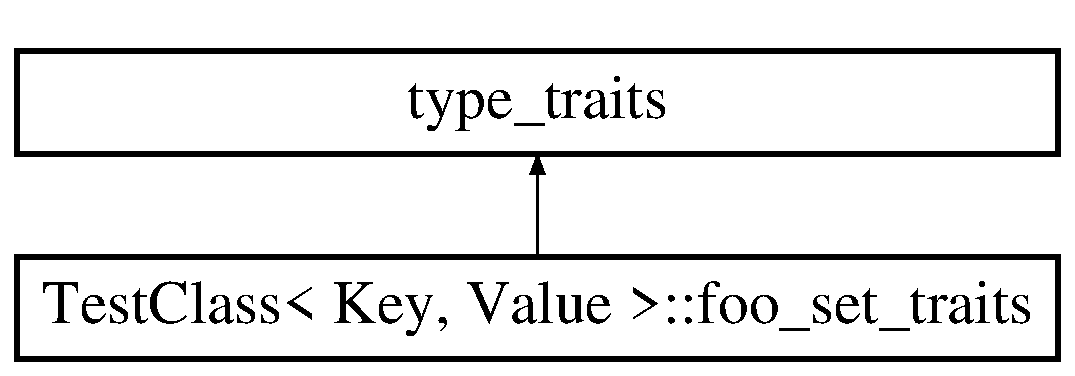
\includegraphics[height=2.000000cm]{struct_test_class_1_1foo__set__traits}
\end{center}
\end{figure}
\subsection*{Classes}
\begin{DoxyCompactItemize}
\item 
struct \hyperlink{struct_test_class_1_1foo__set__traits_1_1ordered__list__traits}{ordered\+\_\+list\+\_\+traits}
\end{DoxyCompactItemize}
\subsection*{Public Types}
\begin{DoxyCompactItemize}
\item 
typedef cds\+::container\+::michael\+\_\+list\+\_\+tag \hyperlink{struct_test_class_1_1foo__set__traits_a9cbc3585bd646618faf9f6a28d5a1133}{ordered\+\_\+list}
\item 
typedef struct \hyperlink{struct_test_class_1_1s__hash}{s\+\_\+hash}$<$ Key $>$ \hyperlink{struct_test_class_1_1foo__set__traits_a5e8da11bd322076d626508eb728c8518}{hash}
\end{DoxyCompactItemize}


\subsection{Member Typedef Documentation}
\hypertarget{struct_test_class_1_1foo__set__traits_a5e8da11bd322076d626508eb728c8518}{}\index{Test\+Class\+::foo\+\_\+set\+\_\+traits@{Test\+Class\+::foo\+\_\+set\+\_\+traits}!hash@{hash}}
\index{hash@{hash}!Test\+Class\+::foo\+\_\+set\+\_\+traits@{Test\+Class\+::foo\+\_\+set\+\_\+traits}}
\subsubsection[{hash}]{\setlength{\rightskip}{0pt plus 5cm}template$<$class Key, class Value$>$ typedef struct {\bf s\+\_\+hash}$<$ Key $>$ {\bf Test\+Class}$<$ Key, {\bf Value} $>$\+::{\bf foo\+\_\+set\+\_\+traits\+::hash}}\label{struct_test_class_1_1foo__set__traits_a5e8da11bd322076d626508eb728c8518}
\hypertarget{struct_test_class_1_1foo__set__traits_a9cbc3585bd646618faf9f6a28d5a1133}{}\index{Test\+Class\+::foo\+\_\+set\+\_\+traits@{Test\+Class\+::foo\+\_\+set\+\_\+traits}!ordered\+\_\+list@{ordered\+\_\+list}}
\index{ordered\+\_\+list@{ordered\+\_\+list}!Test\+Class\+::foo\+\_\+set\+\_\+traits@{Test\+Class\+::foo\+\_\+set\+\_\+traits}}
\subsubsection[{ordered\+\_\+list}]{\setlength{\rightskip}{0pt plus 5cm}template$<$class Key, class Value$>$ typedef cds\+::container\+::michael\+\_\+list\+\_\+tag {\bf Test\+Class}$<$ Key, {\bf Value} $>$\+::{\bf foo\+\_\+set\+\_\+traits\+::ordered\+\_\+list}}\label{struct_test_class_1_1foo__set__traits_a9cbc3585bd646618faf9f6a28d5a1133}


The documentation for this struct was generated from the following file\+:\begin{DoxyCompactItemize}
\item 
tervel/tests/hash\+\_\+map/api/\hyperlink{cds__split__map_8h}{cds\+\_\+split\+\_\+map.\+h}\end{DoxyCompactItemize}

\hypertarget{classtervel_1_1containers_1_1wf_1_1_hash_map_1_1_force_expand_op}{}\section{tervel\+:\+:containers\+:\+:wf\+:\+:Hash\+Map$<$ Key, Value, Functor $>$\+:\+:Force\+Expand\+Op Class Reference}
\label{classtervel_1_1containers_1_1wf_1_1_hash_map_1_1_force_expand_op}\index{tervel\+::containers\+::wf\+::\+Hash\+Map$<$ Key, Value, Functor $>$\+::\+Force\+Expand\+Op@{tervel\+::containers\+::wf\+::\+Hash\+Map$<$ Key, Value, Functor $>$\+::\+Force\+Expand\+Op}}


T\+O\+D\+O(steven)\+: add description T\+O\+D\+O(steven)\+: move into a file.  


Inheritance diagram for tervel\+:\+:containers\+:\+:wf\+:\+:Hash\+Map$<$ Key, Value, Functor $>$\+:\+:Force\+Expand\+Op\+:\begin{figure}[H]
\begin{center}
\leavevmode
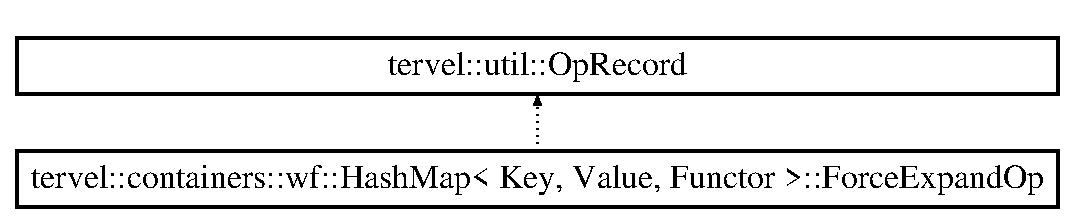
\includegraphics[height=2.000000cm]{classtervel_1_1containers_1_1wf_1_1_hash_map_1_1_force_expand_op}
\end{center}
\end{figure}
\subsection*{Public Member Functions}
\begin{DoxyCompactItemize}
\item 
\hyperlink{classtervel_1_1containers_1_1wf_1_1_hash_map_1_1_force_expand_op_aa7213b3c1c5d4216eabc96771542f59c}{Force\+Expand\+Op} (\hyperlink{classtervel_1_1containers_1_1wf_1_1_hash_map}{Hash\+Map} $\ast$map, \hyperlink{classtervel_1_1containers_1_1wf_1_1_hash_map_ab2c04cbf19034689a795208e0108fe8a}{Location} $\ast$loc, size\+\_\+t depth)
\item 
void \hyperlink{classtervel_1_1containers_1_1wf_1_1_hash_map_1_1_force_expand_op_adfe48adab3158c1e81119a2ff369e3d8}{help\+\_\+complete} ()
\begin{DoxyCompactList}\small\item\em Implementations of this function that upon its return the operation described in the Op\+Record has been completed. \end{DoxyCompactList}\end{DoxyCompactItemize}
\subsection*{Private Attributes}
\begin{DoxyCompactItemize}
\item 
\hyperlink{classtervel_1_1containers_1_1wf_1_1_hash_map}{Hash\+Map} $\ast$ \hyperlink{classtervel_1_1containers_1_1wf_1_1_hash_map_1_1_force_expand_op_a6d1c762e111e8324c9fcaf56354575e1}{map\+\_\+} \{nullptr\}
\item 
\hyperlink{classtervel_1_1containers_1_1wf_1_1_hash_map_ab2c04cbf19034689a795208e0108fe8a}{Location} $\ast$ \hyperlink{classtervel_1_1containers_1_1wf_1_1_hash_map_1_1_force_expand_op_a4f6bd52ceb03f190143e389f60714a53}{loc\+\_\+} \{nullptr\}
\item 
size\+\_\+t \hyperlink{classtervel_1_1containers_1_1wf_1_1_hash_map_1_1_force_expand_op_a089cd031b862f5bafb70882399148174}{depth\+\_\+} \{0\}
\end{DoxyCompactItemize}
\subsection*{Friends}
\begin{DoxyCompactItemize}
\item 
class \hyperlink{classtervel_1_1containers_1_1wf_1_1_hash_map_1_1_force_expand_op_ab6054287e6f409207af3fa16e49046ad}{Hash\+Map}
\end{DoxyCompactItemize}
\subsection*{Additional Inherited Members}


\subsection{Detailed Description}
\subsubsection*{template$<$class Key, class Value, class Functor = default\+\_\+functor$<$\+Key, Value$>$$>$class tervel\+::containers\+::wf\+::\+Hash\+Map$<$ Key, Value, Functor $>$\+::\+Force\+Expand\+Op}

T\+O\+D\+O(steven)\+: add description T\+O\+D\+O(steven)\+: move into a file. 

\subsection{Constructor \& Destructor Documentation}
\hypertarget{classtervel_1_1containers_1_1wf_1_1_hash_map_1_1_force_expand_op_aa7213b3c1c5d4216eabc96771542f59c}{}\index{tervel\+::containers\+::wf\+::\+Hash\+Map\+::\+Force\+Expand\+Op@{tervel\+::containers\+::wf\+::\+Hash\+Map\+::\+Force\+Expand\+Op}!Force\+Expand\+Op@{Force\+Expand\+Op}}
\index{Force\+Expand\+Op@{Force\+Expand\+Op}!tervel\+::containers\+::wf\+::\+Hash\+Map\+::\+Force\+Expand\+Op@{tervel\+::containers\+::wf\+::\+Hash\+Map\+::\+Force\+Expand\+Op}}
\subsubsection[{Force\+Expand\+Op(\+Hash\+Map $\ast$map, Location $\ast$loc, size\+\_\+t depth)}]{\setlength{\rightskip}{0pt plus 5cm}template$<$class Key , class Value , class Functor  = default\+\_\+functor$<$\+Key, Value$>$$>$ {\bf tervel\+::containers\+::wf\+::\+Hash\+Map}$<$ Key, {\bf Value}, Functor $>$\+::Force\+Expand\+Op\+::\+Force\+Expand\+Op (
\begin{DoxyParamCaption}
\item[{{\bf Hash\+Map} $\ast$}]{map, }
\item[{{\bf Location} $\ast$}]{loc, }
\item[{size\+\_\+t}]{depth}
\end{DoxyParamCaption}
)\hspace{0.3cm}{\ttfamily [inline]}}\label{classtervel_1_1containers_1_1wf_1_1_hash_map_1_1_force_expand_op_aa7213b3c1c5d4216eabc96771542f59c}


\subsection{Member Function Documentation}
\hypertarget{classtervel_1_1containers_1_1wf_1_1_hash_map_1_1_force_expand_op_adfe48adab3158c1e81119a2ff369e3d8}{}\index{tervel\+::containers\+::wf\+::\+Hash\+Map\+::\+Force\+Expand\+Op@{tervel\+::containers\+::wf\+::\+Hash\+Map\+::\+Force\+Expand\+Op}!help\+\_\+complete@{help\+\_\+complete}}
\index{help\+\_\+complete@{help\+\_\+complete}!tervel\+::containers\+::wf\+::\+Hash\+Map\+::\+Force\+Expand\+Op@{tervel\+::containers\+::wf\+::\+Hash\+Map\+::\+Force\+Expand\+Op}}
\subsubsection[{help\+\_\+complete()}]{\setlength{\rightskip}{0pt plus 5cm}template$<$class Key , class Value , class Functor  = default\+\_\+functor$<$\+Key, Value$>$$>$ void {\bf tervel\+::containers\+::wf\+::\+Hash\+Map}$<$ Key, {\bf Value}, Functor $>$\+::Force\+Expand\+Op\+::help\+\_\+complete (
\begin{DoxyParamCaption}
{}
\end{DoxyParamCaption}
)\hspace{0.3cm}{\ttfamily [inline]}, {\ttfamily [virtual]}}\label{classtervel_1_1containers_1_1wf_1_1_hash_map_1_1_force_expand_op_adfe48adab3158c1e81119a2ff369e3d8}


Implementations of this function that upon its return the operation described in the Op\+Record has been completed. 

As such it must be thread-\/safe and the extending class must contain all the information necessary to complete the operation. 

Implements \hyperlink{classtervel_1_1util_1_1_op_record_aa75ab39688a8d4cceb6a1ef0409537c0}{tervel\+::util\+::\+Op\+Record}.



\subsection{Friends And Related Function Documentation}
\hypertarget{classtervel_1_1containers_1_1wf_1_1_hash_map_1_1_force_expand_op_ab6054287e6f409207af3fa16e49046ad}{}\index{tervel\+::containers\+::wf\+::\+Hash\+Map\+::\+Force\+Expand\+Op@{tervel\+::containers\+::wf\+::\+Hash\+Map\+::\+Force\+Expand\+Op}!Hash\+Map@{Hash\+Map}}
\index{Hash\+Map@{Hash\+Map}!tervel\+::containers\+::wf\+::\+Hash\+Map\+::\+Force\+Expand\+Op@{tervel\+::containers\+::wf\+::\+Hash\+Map\+::\+Force\+Expand\+Op}}
\subsubsection[{Hash\+Map}]{\setlength{\rightskip}{0pt plus 5cm}template$<$class Key , class Value , class Functor  = default\+\_\+functor$<$\+Key, Value$>$$>$ friend class {\bf Hash\+Map}\hspace{0.3cm}{\ttfamily [friend]}}\label{classtervel_1_1containers_1_1wf_1_1_hash_map_1_1_force_expand_op_ab6054287e6f409207af3fa16e49046ad}


\subsection{Member Data Documentation}
\hypertarget{classtervel_1_1containers_1_1wf_1_1_hash_map_1_1_force_expand_op_a089cd031b862f5bafb70882399148174}{}\index{tervel\+::containers\+::wf\+::\+Hash\+Map\+::\+Force\+Expand\+Op@{tervel\+::containers\+::wf\+::\+Hash\+Map\+::\+Force\+Expand\+Op}!depth\+\_\+@{depth\+\_\+}}
\index{depth\+\_\+@{depth\+\_\+}!tervel\+::containers\+::wf\+::\+Hash\+Map\+::\+Force\+Expand\+Op@{tervel\+::containers\+::wf\+::\+Hash\+Map\+::\+Force\+Expand\+Op}}
\subsubsection[{depth\+\_\+}]{\setlength{\rightskip}{0pt plus 5cm}template$<$class Key , class Value , class Functor  = default\+\_\+functor$<$\+Key, Value$>$$>$ size\+\_\+t {\bf tervel\+::containers\+::wf\+::\+Hash\+Map}$<$ Key, {\bf Value}, Functor $>$\+::Force\+Expand\+Op\+::depth\+\_\+ \{0\}\hspace{0.3cm}{\ttfamily [private]}}\label{classtervel_1_1containers_1_1wf_1_1_hash_map_1_1_force_expand_op_a089cd031b862f5bafb70882399148174}
\hypertarget{classtervel_1_1containers_1_1wf_1_1_hash_map_1_1_force_expand_op_a4f6bd52ceb03f190143e389f60714a53}{}\index{tervel\+::containers\+::wf\+::\+Hash\+Map\+::\+Force\+Expand\+Op@{tervel\+::containers\+::wf\+::\+Hash\+Map\+::\+Force\+Expand\+Op}!loc\+\_\+@{loc\+\_\+}}
\index{loc\+\_\+@{loc\+\_\+}!tervel\+::containers\+::wf\+::\+Hash\+Map\+::\+Force\+Expand\+Op@{tervel\+::containers\+::wf\+::\+Hash\+Map\+::\+Force\+Expand\+Op}}
\subsubsection[{loc\+\_\+}]{\setlength{\rightskip}{0pt plus 5cm}template$<$class Key , class Value , class Functor  = default\+\_\+functor$<$\+Key, Value$>$$>$ {\bf Location}$\ast$ {\bf tervel\+::containers\+::wf\+::\+Hash\+Map}$<$ Key, {\bf Value}, Functor $>$\+::Force\+Expand\+Op\+::loc\+\_\+ \{nullptr\}\hspace{0.3cm}{\ttfamily [private]}}\label{classtervel_1_1containers_1_1wf_1_1_hash_map_1_1_force_expand_op_a4f6bd52ceb03f190143e389f60714a53}
\hypertarget{classtervel_1_1containers_1_1wf_1_1_hash_map_1_1_force_expand_op_a6d1c762e111e8324c9fcaf56354575e1}{}\index{tervel\+::containers\+::wf\+::\+Hash\+Map\+::\+Force\+Expand\+Op@{tervel\+::containers\+::wf\+::\+Hash\+Map\+::\+Force\+Expand\+Op}!map\+\_\+@{map\+\_\+}}
\index{map\+\_\+@{map\+\_\+}!tervel\+::containers\+::wf\+::\+Hash\+Map\+::\+Force\+Expand\+Op@{tervel\+::containers\+::wf\+::\+Hash\+Map\+::\+Force\+Expand\+Op}}
\subsubsection[{map\+\_\+}]{\setlength{\rightskip}{0pt plus 5cm}template$<$class Key , class Value , class Functor  = default\+\_\+functor$<$\+Key, Value$>$$>$ {\bf Hash\+Map}$\ast$ {\bf tervel\+::containers\+::wf\+::\+Hash\+Map}$<$ Key, {\bf Value}, Functor $>$\+::Force\+Expand\+Op\+::map\+\_\+ \{nullptr\}\hspace{0.3cm}{\ttfamily [private]}}\label{classtervel_1_1containers_1_1wf_1_1_hash_map_1_1_force_expand_op_a6d1c762e111e8324c9fcaf56354575e1}


The documentation for this class was generated from the following file\+:\begin{DoxyCompactItemize}
\item 
tervel/containers/wf/hash-\/map/\hyperlink{wf__hash__map_8h}{wf\+\_\+hash\+\_\+map.\+h}\end{DoxyCompactItemize}

\hypertarget{struct_test_class_1_1functor}{}\section{Test\+Class$<$ Key, Value $>$\+:\+:functor Struct Reference}
\label{struct_test_class_1_1functor}\index{Test\+Class$<$ Key, Value $>$\+::functor@{Test\+Class$<$ Key, Value $>$\+::functor}}
\subsection*{Public Member Functions}
\begin{DoxyCompactItemize}
\item 
void \hyperlink{struct_test_class_1_1functor_ac6890291dc692c73faaa31bee690b41e}{operator()} (std\+::pair$<$ Key, \hyperlink{hash__map_2test_object_8h_ad777bf08d8e2b01df17ba5e3c51ae11f}{Value} $>$ pair)
\item 
bool \hyperlink{struct_test_class_1_1functor_aeb074051580e7abcbe0507018d927adb}{get\+Value} (\hyperlink{hash__map_2test_object_8h_ad777bf08d8e2b01df17ba5e3c51ae11f}{Value} \&val)
\item 
void \hyperlink{struct_test_class_1_1functor_ac6890291dc692c73faaa31bee690b41e}{operator()} (std\+::pair$<$ Key, \hyperlink{hash__map_2test_object_8h_ad777bf08d8e2b01df17ba5e3c51ae11f}{Value} $>$ pair)
\item 
bool \hyperlink{struct_test_class_1_1functor_aeb074051580e7abcbe0507018d927adb}{get\+Value} (\hyperlink{hash__map_2test_object_8h_ad777bf08d8e2b01df17ba5e3c51ae11f}{Value} \&val)
\end{DoxyCompactItemize}
\subsection*{Public Attributes}
\begin{DoxyCompactItemize}
\item 
\hyperlink{hash__map_2test_object_8h_ad777bf08d8e2b01df17ba5e3c51ae11f}{Value} \hyperlink{struct_test_class_1_1functor_ae8901ceb7e534ecf91007659aef7ab70}{curr\+\_\+value}
\item 
bool \hyperlink{struct_test_class_1_1functor_aac45799e70b923c7ebd6b1e3aa5ad933}{res}
\end{DoxyCompactItemize}


\subsection{Member Function Documentation}
\hypertarget{struct_test_class_1_1functor_aeb074051580e7abcbe0507018d927adb}{}\index{Test\+Class\+::functor@{Test\+Class\+::functor}!get\+Value@{get\+Value}}
\index{get\+Value@{get\+Value}!Test\+Class\+::functor@{Test\+Class\+::functor}}
\subsubsection[{get\+Value(\+Value \&val)}]{\setlength{\rightskip}{0pt plus 5cm}template$<$class Key, class Value$>$ bool {\bf Test\+Class}$<$ Key, {\bf Value} $>$\+::functor\+::get\+Value (
\begin{DoxyParamCaption}
\item[{{\bf Value} \&}]{val}
\end{DoxyParamCaption}
)\hspace{0.3cm}{\ttfamily [inline]}}\label{struct_test_class_1_1functor_aeb074051580e7abcbe0507018d927adb}
\hypertarget{struct_test_class_1_1functor_aeb074051580e7abcbe0507018d927adb}{}\index{Test\+Class\+::functor@{Test\+Class\+::functor}!get\+Value@{get\+Value}}
\index{get\+Value@{get\+Value}!Test\+Class\+::functor@{Test\+Class\+::functor}}
\subsubsection[{get\+Value(\+Value \&val)}]{\setlength{\rightskip}{0pt plus 5cm}template$<$class Key, class Value$>$ bool {\bf Test\+Class}$<$ Key, {\bf Value} $>$\+::functor\+::get\+Value (
\begin{DoxyParamCaption}
\item[{{\bf Value} \&}]{val}
\end{DoxyParamCaption}
)\hspace{0.3cm}{\ttfamily [inline]}}\label{struct_test_class_1_1functor_aeb074051580e7abcbe0507018d927adb}
\hypertarget{struct_test_class_1_1functor_ac6890291dc692c73faaa31bee690b41e}{}\index{Test\+Class\+::functor@{Test\+Class\+::functor}!operator()@{operator()}}
\index{operator()@{operator()}!Test\+Class\+::functor@{Test\+Class\+::functor}}
\subsubsection[{operator()(std\+::pair$<$ Key, Value $>$ pair)}]{\setlength{\rightskip}{0pt plus 5cm}template$<$class Key, class Value$>$ void {\bf Test\+Class}$<$ Key, {\bf Value} $>$\+::functor\+::operator() (
\begin{DoxyParamCaption}
\item[{std\+::pair$<$ Key, {\bf Value} $>$}]{pair}
\end{DoxyParamCaption}
)\hspace{0.3cm}{\ttfamily [inline]}}\label{struct_test_class_1_1functor_ac6890291dc692c73faaa31bee690b41e}
\hypertarget{struct_test_class_1_1functor_ac6890291dc692c73faaa31bee690b41e}{}\index{Test\+Class\+::functor@{Test\+Class\+::functor}!operator()@{operator()}}
\index{operator()@{operator()}!Test\+Class\+::functor@{Test\+Class\+::functor}}
\subsubsection[{operator()(std\+::pair$<$ Key, Value $>$ pair)}]{\setlength{\rightskip}{0pt plus 5cm}template$<$class Key, class Value$>$ void {\bf Test\+Class}$<$ Key, {\bf Value} $>$\+::functor\+::operator() (
\begin{DoxyParamCaption}
\item[{std\+::pair$<$ Key, {\bf Value} $>$}]{pair}
\end{DoxyParamCaption}
)\hspace{0.3cm}{\ttfamily [inline]}}\label{struct_test_class_1_1functor_ac6890291dc692c73faaa31bee690b41e}


\subsection{Member Data Documentation}
\hypertarget{struct_test_class_1_1functor_ae8901ceb7e534ecf91007659aef7ab70}{}\index{Test\+Class\+::functor@{Test\+Class\+::functor}!curr\+\_\+value@{curr\+\_\+value}}
\index{curr\+\_\+value@{curr\+\_\+value}!Test\+Class\+::functor@{Test\+Class\+::functor}}
\subsubsection[{curr\+\_\+value}]{\setlength{\rightskip}{0pt plus 5cm}template$<$class Key, class Value$>$ {\bf Value} {\bf Test\+Class}$<$ Key, {\bf Value} $>$\+::functor\+::curr\+\_\+value}\label{struct_test_class_1_1functor_ae8901ceb7e534ecf91007659aef7ab70}
\hypertarget{struct_test_class_1_1functor_aac45799e70b923c7ebd6b1e3aa5ad933}{}\index{Test\+Class\+::functor@{Test\+Class\+::functor}!res@{res}}
\index{res@{res}!Test\+Class\+::functor@{Test\+Class\+::functor}}
\subsubsection[{res}]{\setlength{\rightskip}{0pt plus 5cm}template$<$class Key, class Value$>$ bool {\bf Test\+Class}$<$ Key, {\bf Value} $>$\+::functor\+::res}\label{struct_test_class_1_1functor_aac45799e70b923c7ebd6b1e3aa5ad933}


The documentation for this struct was generated from the following files\+:\begin{DoxyCompactItemize}
\item 
tervel/tests/hash\+\_\+map/api/\hyperlink{cds__michael__map_8h}{cds\+\_\+michael\+\_\+map.\+h}\item 
tervel/tests/hash\+\_\+map/api/\hyperlink{cds__split__map_8h}{cds\+\_\+split\+\_\+map.\+h}\end{DoxyCompactItemize}

\hypertarget{struct_test_class_1_1map__traits_1_1hash}{}\section{Test\+Class$<$ Key, Value $>$\+:\+:map\+\_\+traits\+:\+:hash Struct Reference}
\label{struct_test_class_1_1map__traits_1_1hash}\index{Test\+Class$<$ Key, Value $>$\+::map\+\_\+traits\+::hash@{Test\+Class$<$ Key, Value $>$\+::map\+\_\+traits\+::hash}}


{\ttfamily \#include $<$cds\+\_\+michael\+\_\+map.\+h$>$}

\subsection*{Public Member Functions}
\begin{DoxyCompactItemize}
\item 
size\+\_\+t \hyperlink{struct_test_class_1_1map__traits_1_1hash_a327afe44c2bb0e61f3a31006d1272ddb}{operator()} (const Key \&k) const 
\end{DoxyCompactItemize}


\subsection{Member Function Documentation}
\hypertarget{struct_test_class_1_1map__traits_1_1hash_a327afe44c2bb0e61f3a31006d1272ddb}{}\index{Test\+Class\+::map\+\_\+traits\+::hash@{Test\+Class\+::map\+\_\+traits\+::hash}!operator()@{operator()}}
\index{operator()@{operator()}!Test\+Class\+::map\+\_\+traits\+::hash@{Test\+Class\+::map\+\_\+traits\+::hash}}
\subsubsection[{operator()(const Key \&k) const }]{\setlength{\rightskip}{0pt plus 5cm}template$<$class Key, class Value$>$ size\+\_\+t {\bf Test\+Class}$<$ Key, {\bf Value} $>$\+::map\+\_\+traits\+::hash\+::operator() (
\begin{DoxyParamCaption}
\item[{const Key \&}]{k}
\end{DoxyParamCaption}
) const\hspace{0.3cm}{\ttfamily [inline]}}\label{struct_test_class_1_1map__traits_1_1hash_a327afe44c2bb0e61f3a31006d1272ddb}


The documentation for this struct was generated from the following file\+:\begin{DoxyCompactItemize}
\item 
tervel/tests/hash\+\_\+map/api/\hyperlink{cds__michael__map_8h}{cds\+\_\+michael\+\_\+map.\+h}\end{DoxyCompactItemize}

\hypertarget{classtervel_1_1containers_1_1wf_1_1_hash_map}{}\section{tervel\+:\+:containers\+:\+:wf\+:\+:Hash\+Map$<$ Key, Value, Functor $>$ Class Template Reference}
\label{classtervel_1_1containers_1_1wf_1_1_hash_map}\index{tervel\+::containers\+::wf\+::\+Hash\+Map$<$ Key, Value, Functor $>$@{tervel\+::containers\+::wf\+::\+Hash\+Map$<$ Key, Value, Functor $>$}}


A wait-\/free hash map implementation.  




{\ttfamily \#include $<$wf\+\_\+hash\+\_\+map.\+h$>$}

\subsection*{Classes}
\begin{DoxyCompactItemize}
\item 
class \hyperlink{classtervel_1_1containers_1_1wf_1_1_hash_map_1_1_array_node}{Array\+Node}
\begin{DoxyCompactList}\small\item\em This class is used to hold the secondary array structure. \end{DoxyCompactList}\item 
class \hyperlink{classtervel_1_1containers_1_1wf_1_1_hash_map_1_1_data_node}{Data\+Node}
\begin{DoxyCompactList}\small\item\em This class is used to hold a key and value pair. \end{DoxyCompactList}\item 
class \hyperlink{classtervel_1_1containers_1_1wf_1_1_hash_map_1_1_force_expand_op}{Force\+Expand\+Op}
\begin{DoxyCompactList}\small\item\em T\+O\+D\+O(steven)\+: add description T\+O\+D\+O(steven)\+: move into a file. \end{DoxyCompactList}\item 
class \hyperlink{classtervel_1_1containers_1_1wf_1_1_hash_map_1_1_node}{Node}
\begin{DoxyCompactList}\small\item\em This class is used to differentiate between data\+\_\+nodes and array\+\_\+nodes/. \end{DoxyCompactList}\item 
class \hyperlink{classtervel_1_1containers_1_1wf_1_1_hash_map_1_1_value_accessor}{Value\+Accessor}
\begin{DoxyCompactList}\small\item\em This class is used to safe guard access to values. \end{DoxyCompactList}\end{DoxyCompactItemize}
\subsection*{Public Member Functions}
\begin{DoxyCompactItemize}
\item 
\hyperlink{classtervel_1_1containers_1_1wf_1_1_hash_map_ad8c150cd36ed719afb858430337f1c62}{Hash\+Map} (uint64\+\_\+t capacity, uint64\+\_\+t expansion\+\_\+rate=3)
\item 
\hyperlink{classtervel_1_1containers_1_1wf_1_1_hash_map_ae794cb0541447e72830673a22f541ca8}{$\sim$\+Hash\+Map} ()
\begin{DoxyCompactList}\small\item\em Not Thread Safe! May create a very large stack! Note\+: should implement a better way... \end{DoxyCompactList}\item 
bool \hyperlink{classtervel_1_1containers_1_1wf_1_1_hash_map_a4c1495c1d9bcdef760f0a4d973778d57}{at} (Key key, \hyperlink{classtervel_1_1containers_1_1wf_1_1_hash_map_1_1_value_accessor}{Value\+Accessor} \&va)
\begin{DoxyCompactList}\small\item\em This function returns true and initializes the passed \hyperlink{classtervel_1_1containers_1_1wf_1_1_hash_map_1_1_value_accessor}{Value\+Accessor} if the key exists in the hash map. \end{DoxyCompactList}\item 
bool \hyperlink{classtervel_1_1containers_1_1wf_1_1_hash_map_aa987d6abf872d3fb51a714fa9c3da047}{insert} (Key key, \hyperlink{hash__map_2test_object_8h_ad777bf08d8e2b01df17ba5e3c51ae11f}{Value} value)
\begin{DoxyCompactList}\small\item\em This function returns true if the key value pair was successfully inserted. \end{DoxyCompactList}\item 
bool \hyperlink{classtervel_1_1containers_1_1wf_1_1_hash_map_ad4c3355a93bdec5af4d8dba02b9bd02a}{remove} (Key key)
\begin{DoxyCompactList}\small\item\em Attempts to remove a key/value pair from the hash map Returns false in the event the key is not in the hash map or if the access\+\_\+counter is non-\/zero. \end{DoxyCompactList}\item 
size\+\_\+t \hyperlink{classtervel_1_1containers_1_1wf_1_1_hash_map_a2fb368a522433b4a96c8d4ac7feb7a78}{size} ()
\item 
uint64\+\_\+t \hyperlink{classtervel_1_1containers_1_1wf_1_1_hash_map_a8e8d0c8976e57161982b2690429c7a21}{get\+\_\+position} (Key \&key, size\+\_\+t depth)
\item 
uint64\+\_\+t \hyperlink{classtervel_1_1containers_1_1wf_1_1_hash_map_a6612d9ecf9fa6707d6f5f6cc9aa59613}{max\+\_\+depth} ()
\item 
void \hyperlink{classtervel_1_1containers_1_1wf_1_1_hash_map_aef0328afe3b270b14f6345e76aff9ef7}{print\+\_\+key} (Key \&key)
\begin{DoxyCompactList}\small\item\em Outputs the positions a key belongs in at each depth. \end{DoxyCompactList}\end{DoxyCompactItemize}
\subsection*{Private Types}
\begin{DoxyCompactItemize}
\item 
typedef std\+::atomic$<$ \hyperlink{classtervel_1_1containers_1_1wf_1_1_hash_map_1_1_node}{Node} $\ast$ $>$ \hyperlink{classtervel_1_1containers_1_1wf_1_1_hash_map_ab2c04cbf19034689a795208e0108fe8a}{Location}
\end{DoxyCompactItemize}
\subsection*{Private Member Functions}
\begin{DoxyCompactItemize}
\item 
void \hyperlink{classtervel_1_1containers_1_1wf_1_1_hash_map_a16ae6d201452512192fdca6e2edfb103}{expand\+\_\+map} (\hyperlink{classtervel_1_1containers_1_1wf_1_1_hash_map_ab2c04cbf19034689a795208e0108fe8a}{Location} $\ast$loc, \hyperlink{classtervel_1_1containers_1_1wf_1_1_hash_map_1_1_node}{Node} $\ast$curr\+\_\+value, size\+\_\+t depth)
\begin{DoxyCompactList}\small\item\em Increases the capacity of the hash map by replacing a data node reference with a reference to an array node containing a reference to that data node. \end{DoxyCompactList}\item 
bool \hyperlink{classtervel_1_1containers_1_1wf_1_1_hash_map_ad20d1a66ecbec92076502223116708e4}{hp\+\_\+watch\+\_\+and\+\_\+get\+\_\+value} (\hyperlink{classtervel_1_1containers_1_1wf_1_1_hash_map_ab2c04cbf19034689a795208e0108fe8a}{Location} $\ast$loc, \hyperlink{classtervel_1_1containers_1_1wf_1_1_hash_map_1_1_node}{Node} $\ast$\&value)
\begin{DoxyCompactList}\small\item\em This is a wrapper for hazard pointers. \end{DoxyCompactList}\item 
void \hyperlink{classtervel_1_1containers_1_1wf_1_1_hash_map_aa69a1e4365aa684f19af2b98fe0a663a}{hp\+\_\+unwatch} ()
\end{DoxyCompactItemize}
\subsection*{Private Attributes}
\begin{DoxyCompactItemize}
\item 
const size\+\_\+t \hyperlink{classtervel_1_1containers_1_1wf_1_1_hash_map_a33e402d5fcf528ee13dbe5aa3f893fa2}{primary\+\_\+array\+\_\+size\+\_\+}
\item 
const size\+\_\+t \hyperlink{classtervel_1_1containers_1_1wf_1_1_hash_map_abaa36dc12509164a3c9612666a4eacbc}{primary\+\_\+array\+\_\+pow\+\_\+}
\item 
const size\+\_\+t \hyperlink{classtervel_1_1containers_1_1wf_1_1_hash_map_ac9a43fdb98927d0147a1240bd882e70b}{secondary\+\_\+array\+\_\+size\+\_\+}
\item 
const size\+\_\+t \hyperlink{classtervel_1_1containers_1_1wf_1_1_hash_map_a0db3b6f46ecf2ac2c243ee76edf0a4f5}{secondary\+\_\+array\+\_\+pow\+\_\+}
\item 
std\+::atomic$<$ uint64\+\_\+t $>$ \hyperlink{classtervel_1_1containers_1_1wf_1_1_hash_map_a88bcdcb8728735910311f62e99027385}{size\+\_\+}
\item 
std\+::unique\+\_\+ptr$<$ \hyperlink{classtervel_1_1containers_1_1wf_1_1_hash_map_ab2c04cbf19034689a795208e0108fe8a}{Location}\mbox{[}$\,$\mbox{]}$>$ \hyperlink{classtervel_1_1containers_1_1wf_1_1_hash_map_a501a15b166513ae18873d6d1d3da71a4}{primary\+\_\+array\+\_\+}
\end{DoxyCompactItemize}
\subsection*{Friends}
\begin{DoxyCompactItemize}
\item 
class \hyperlink{classtervel_1_1containers_1_1wf_1_1_hash_map_a6db9d28bd448a131448276ee03de1e6d}{Node}
\item 
class \hyperlink{classtervel_1_1containers_1_1wf_1_1_hash_map_a92fd79231cf52565db2b541bf8b96039}{Force\+Expand\+Op}
\end{DoxyCompactItemize}


\subsection{Detailed Description}
\subsubsection*{template$<$class Key, class Value, class Functor = default\+\_\+functor$<$\+Key, Value$>$$>$class tervel\+::containers\+::wf\+::\+Hash\+Map$<$ Key, Value, Functor $>$}

A wait-\/free hash map implementation. 

T\+O\+D\+O(steven)\+: Provide general overview

Functor should have the following functions\+: -\/\+Key hash(\+Key k) (where hash(a) == (hash(b) implies a == b -\/bool key\+\_\+equals (Key a, Key b) Important Note\+: the hashed value of keys will be passed in. 

\subsection{Member Typedef Documentation}
\hypertarget{classtervel_1_1containers_1_1wf_1_1_hash_map_ab2c04cbf19034689a795208e0108fe8a}{}\index{tervel\+::containers\+::wf\+::\+Hash\+Map@{tervel\+::containers\+::wf\+::\+Hash\+Map}!Location@{Location}}
\index{Location@{Location}!tervel\+::containers\+::wf\+::\+Hash\+Map@{tervel\+::containers\+::wf\+::\+Hash\+Map}}
\subsubsection[{Location}]{\setlength{\rightskip}{0pt plus 5cm}template$<$class Key , class Value , class Functor  = default\+\_\+functor$<$\+Key, Value$>$$>$ typedef std\+::atomic$<${\bf Node} $\ast$$>$ {\bf tervel\+::containers\+::wf\+::\+Hash\+Map}$<$ Key, {\bf Value}, Functor $>$\+::{\bf Location}\hspace{0.3cm}{\ttfamily [private]}}\label{classtervel_1_1containers_1_1wf_1_1_hash_map_ab2c04cbf19034689a795208e0108fe8a}


\subsection{Constructor \& Destructor Documentation}
\hypertarget{classtervel_1_1containers_1_1wf_1_1_hash_map_ad8c150cd36ed719afb858430337f1c62}{}\index{tervel\+::containers\+::wf\+::\+Hash\+Map@{tervel\+::containers\+::wf\+::\+Hash\+Map}!Hash\+Map@{Hash\+Map}}
\index{Hash\+Map@{Hash\+Map}!tervel\+::containers\+::wf\+::\+Hash\+Map@{tervel\+::containers\+::wf\+::\+Hash\+Map}}
\subsubsection[{Hash\+Map(uint64\+\_\+t capacity, uint64\+\_\+t expansion\+\_\+rate=3)}]{\setlength{\rightskip}{0pt plus 5cm}template$<$class Key , class Value , class Functor  = default\+\_\+functor$<$\+Key, Value$>$$>$ {\bf tervel\+::containers\+::wf\+::\+Hash\+Map}$<$ Key, {\bf Value}, Functor $>$\+::{\bf Hash\+Map} (
\begin{DoxyParamCaption}
\item[{uint64\+\_\+t}]{capacity, }
\item[{uint64\+\_\+t}]{expansion\+\_\+rate = {\ttfamily 3}}
\end{DoxyParamCaption}
)\hspace{0.3cm}{\ttfamily [inline]}}\label{classtervel_1_1containers_1_1wf_1_1_hash_map_ad8c150cd36ed719afb858430337f1c62}
\hypertarget{classtervel_1_1containers_1_1wf_1_1_hash_map_ae794cb0541447e72830673a22f541ca8}{}\index{tervel\+::containers\+::wf\+::\+Hash\+Map@{tervel\+::containers\+::wf\+::\+Hash\+Map}!````~Hash\+Map@{$\sim$\+Hash\+Map}}
\index{````~Hash\+Map@{$\sim$\+Hash\+Map}!tervel\+::containers\+::wf\+::\+Hash\+Map@{tervel\+::containers\+::wf\+::\+Hash\+Map}}
\subsubsection[{$\sim$\+Hash\+Map()}]{\setlength{\rightskip}{0pt plus 5cm}template$<$class Key , class Value , class Functor  = default\+\_\+functor$<$\+Key, Value$>$$>$ {\bf tervel\+::containers\+::wf\+::\+Hash\+Map}$<$ Key, {\bf Value}, Functor $>$\+::$\sim${\bf Hash\+Map} (
\begin{DoxyParamCaption}
{}
\end{DoxyParamCaption}
)\hspace{0.3cm}{\ttfamily [inline]}}\label{classtervel_1_1containers_1_1wf_1_1_hash_map_ae794cb0541447e72830673a22f541ca8}


Not Thread Safe! May create a very large stack! Note\+: should implement a better way... 

If it is a node type then the node will be freed If it is an array node then the destructor of the array node will free any nodes that are referenced it. This may cause more array node\textquotesingle{}s to be freed. Stack can reach \hyperlink{classtervel_1_1containers_1_1wf_1_1_hash_map_a6612d9ecf9fa6707d6f5f6cc9aa59613}{max\+\_\+depth()} in size. 

\subsection{Member Function Documentation}
\hypertarget{classtervel_1_1containers_1_1wf_1_1_hash_map_a4c1495c1d9bcdef760f0a4d973778d57}{}\index{tervel\+::containers\+::wf\+::\+Hash\+Map@{tervel\+::containers\+::wf\+::\+Hash\+Map}!at@{at}}
\index{at@{at}!tervel\+::containers\+::wf\+::\+Hash\+Map@{tervel\+::containers\+::wf\+::\+Hash\+Map}}
\subsubsection[{at(\+Key key, Value\+Accessor \&va)}]{\setlength{\rightskip}{0pt plus 5cm}template$<$class Key , class Value , class Functor $>$ bool {\bf tervel\+::containers\+::wf\+::\+Hash\+Map}$<$ Key, {\bf Value}, Functor $>$\+::at (
\begin{DoxyParamCaption}
\item[{Key}]{key, }
\item[{{\bf Value\+Accessor} \&}]{va}
\end{DoxyParamCaption}
)}\label{classtervel_1_1containers_1_1wf_1_1_hash_map_a4c1495c1d9bcdef760f0a4d973778d57}


This function returns true and initializes the passed \hyperlink{classtervel_1_1containers_1_1wf_1_1_hash_map_1_1_value_accessor}{Value\+Accessor} if the key exists in the hash map. 

Initializing the \hyperlink{classtervel_1_1containers_1_1wf_1_1_hash_map_1_1_value_accessor}{Value\+Accessor} consists of assigning storing a reference to the associated value and a reference to the access counter. The access counter will have been increased by one. Upon the destruction or re-\/initialization of the \hyperlink{classtervel_1_1containers_1_1wf_1_1_hash_map_1_1_value_accessor}{Value\+Accessor}, the access counter will be decremented.

The sequential complexity of this operation is O(max\+\_\+depth()).


\begin{DoxyParams}{Parameters}
{\em key} & the key to look up \\
\hline
{\em va} & the location to store the address of the value/access\+\_\+counter \\
\hline
\end{DoxyParams}
\begin{DoxyReturn}{Returns}
whether or not the key is present 
\end{DoxyReturn}
\hypertarget{classtervel_1_1containers_1_1wf_1_1_hash_map_a16ae6d201452512192fdca6e2edfb103}{}\index{tervel\+::containers\+::wf\+::\+Hash\+Map@{tervel\+::containers\+::wf\+::\+Hash\+Map}!expand\+\_\+map@{expand\+\_\+map}}
\index{expand\+\_\+map@{expand\+\_\+map}!tervel\+::containers\+::wf\+::\+Hash\+Map@{tervel\+::containers\+::wf\+::\+Hash\+Map}}
\subsubsection[{expand\+\_\+map(\+Location $\ast$loc, Node $\ast$curr\+\_\+value, size\+\_\+t depth)}]{\setlength{\rightskip}{0pt plus 5cm}template$<$class Key , class Value , class Functor $>$ void {\bf tervel\+::containers\+::wf\+::\+Hash\+Map}$<$ Key, {\bf Value}, Functor $>$\+::expand\+\_\+map (
\begin{DoxyParamCaption}
\item[{{\bf Location} $\ast$}]{loc, }
\item[{{\bf Node} $\ast$}]{curr\+\_\+value, }
\item[{size\+\_\+t}]{depth}
\end{DoxyParamCaption}
)\hspace{0.3cm}{\ttfamily [private]}}\label{classtervel_1_1containers_1_1wf_1_1_hash_map_a16ae6d201452512192fdca6e2edfb103}


Increases the capacity of the hash map by replacing a data node reference with a reference to an array node containing a reference to that data node. 


\begin{DoxyParams}{Parameters}
{\em loc} & The location to expand at \\
\hline
{\em curr\+\_\+value} & The current value (data node) at the location \\
\hline
{\em next\+\_\+position} & The position the data node belongs at the next depth. \\
\hline
\end{DoxyParams}
\hypertarget{classtervel_1_1containers_1_1wf_1_1_hash_map_a8e8d0c8976e57161982b2690429c7a21}{}\index{tervel\+::containers\+::wf\+::\+Hash\+Map@{tervel\+::containers\+::wf\+::\+Hash\+Map}!get\+\_\+position@{get\+\_\+position}}
\index{get\+\_\+position@{get\+\_\+position}!tervel\+::containers\+::wf\+::\+Hash\+Map@{tervel\+::containers\+::wf\+::\+Hash\+Map}}
\subsubsection[{get\+\_\+position(\+Key \&key, size\+\_\+t depth)}]{\setlength{\rightskip}{0pt plus 5cm}template$<$class Key , class Value , class Functor $>$ uint64\+\_\+t {\bf tervel\+::containers\+::wf\+::\+Hash\+Map}$<$ Key, {\bf Value}, Functor $>$\+::get\+\_\+position (
\begin{DoxyParamCaption}
\item[{Key \&}]{key, }
\item[{size\+\_\+t}]{depth}
\end{DoxyParamCaption}
)}\label{classtervel_1_1containers_1_1wf_1_1_hash_map_a8e8d0c8976e57161982b2690429c7a21}

\begin{DoxyParams}{Parameters}
{\em key} & The key \\
\hline
{\em depth} & The depth \\
\hline
\end{DoxyParams}
\begin{DoxyReturn}{Returns}
the position this key belongs in at the specified depth. 
\end{DoxyReturn}
\hypertarget{classtervel_1_1containers_1_1wf_1_1_hash_map_aa69a1e4365aa684f19af2b98fe0a663a}{}\index{tervel\+::containers\+::wf\+::\+Hash\+Map@{tervel\+::containers\+::wf\+::\+Hash\+Map}!hp\+\_\+unwatch@{hp\+\_\+unwatch}}
\index{hp\+\_\+unwatch@{hp\+\_\+unwatch}!tervel\+::containers\+::wf\+::\+Hash\+Map@{tervel\+::containers\+::wf\+::\+Hash\+Map}}
\subsubsection[{hp\+\_\+unwatch()}]{\setlength{\rightskip}{0pt plus 5cm}template$<$class Key , class Value , class Functor $>$ void {\bf tervel\+::containers\+::wf\+::\+Hash\+Map}$<$ Key, {\bf Value}, Functor $>$\+::hp\+\_\+unwatch (
\begin{DoxyParamCaption}
{}
\end{DoxyParamCaption}
)\hspace{0.3cm}{\ttfamily [private]}}\label{classtervel_1_1containers_1_1wf_1_1_hash_map_aa69a1e4365aa684f19af2b98fe0a663a}
\hypertarget{classtervel_1_1containers_1_1wf_1_1_hash_map_ad20d1a66ecbec92076502223116708e4}{}\index{tervel\+::containers\+::wf\+::\+Hash\+Map@{tervel\+::containers\+::wf\+::\+Hash\+Map}!hp\+\_\+watch\+\_\+and\+\_\+get\+\_\+value@{hp\+\_\+watch\+\_\+and\+\_\+get\+\_\+value}}
\index{hp\+\_\+watch\+\_\+and\+\_\+get\+\_\+value@{hp\+\_\+watch\+\_\+and\+\_\+get\+\_\+value}!tervel\+::containers\+::wf\+::\+Hash\+Map@{tervel\+::containers\+::wf\+::\+Hash\+Map}}
\subsubsection[{hp\+\_\+watch\+\_\+and\+\_\+get\+\_\+value(\+Location $\ast$loc, Node $\ast$\&value)}]{\setlength{\rightskip}{0pt plus 5cm}template$<$class Key , class Value , class Functor $>$ bool {\bf tervel\+::containers\+::wf\+::\+Hash\+Map}$<$ Key, {\bf Value}, Functor $>$\+::hp\+\_\+watch\+\_\+and\+\_\+get\+\_\+value (
\begin{DoxyParamCaption}
\item[{{\bf Location} $\ast$}]{loc, }
\item[{{\bf Node} $\ast$\&}]{value}
\end{DoxyParamCaption}
)\hspace{0.3cm}{\ttfamily [private]}}\label{classtervel_1_1containers_1_1wf_1_1_hash_map_ad20d1a66ecbec92076502223116708e4}


This is a wrapper for hazard pointers. 

If it returns true then the value has been assigned the current value of loc and it is hazard pointer protected. 
\begin{DoxyParams}{Parameters}
{\em loc} & the location to dereference a \hyperlink{classtervel_1_1containers_1_1wf_1_1_hash_map_1_1_node}{Node} object from \\
\hline
{\em value} & the destination to write the \hyperlink{classtervel_1_1containers_1_1wf_1_1_hash_map_1_1_node}{Node} objet pointer \\
\hline
\end{DoxyParams}
\begin{DoxyReturn}{Returns}
whether or not it was able to dereference and hazard pointer watch a node object. 
\end{DoxyReturn}
\hypertarget{classtervel_1_1containers_1_1wf_1_1_hash_map_aa987d6abf872d3fb51a714fa9c3da047}{}\index{tervel\+::containers\+::wf\+::\+Hash\+Map@{tervel\+::containers\+::wf\+::\+Hash\+Map}!insert@{insert}}
\index{insert@{insert}!tervel\+::containers\+::wf\+::\+Hash\+Map@{tervel\+::containers\+::wf\+::\+Hash\+Map}}
\subsubsection[{insert(\+Key key, Value value)}]{\setlength{\rightskip}{0pt plus 5cm}template$<$class Key , class Value , class Functor $>$ bool {\bf tervel\+::containers\+::wf\+::\+Hash\+Map}$<$ Key, {\bf Value}, Functor $>$\+::insert (
\begin{DoxyParamCaption}
\item[{Key}]{key, }
\item[{{\bf Value}}]{value}
\end{DoxyParamCaption}
)}\label{classtervel_1_1containers_1_1wf_1_1_hash_map_aa987d6abf872d3fb51a714fa9c3da047}


This function returns true if the key value pair was successfully inserted. 

Otherwise it returns false.

A key can fail to insert in the event the key is already present.

The sequential complexity of this operation is O(max\+\_\+depth()).


\begin{DoxyParams}{Parameters}
{\em key} & The key to insert \\
\hline
{\em value} & The key\textquotesingle{}s associated value \\
\hline
\end{DoxyParams}
\begin{DoxyReturn}{Returns}
whether or not the the key/value was inserted 
\end{DoxyReturn}
\hypertarget{classtervel_1_1containers_1_1wf_1_1_hash_map_a6612d9ecf9fa6707d6f5f6cc9aa59613}{}\index{tervel\+::containers\+::wf\+::\+Hash\+Map@{tervel\+::containers\+::wf\+::\+Hash\+Map}!max\+\_\+depth@{max\+\_\+depth}}
\index{max\+\_\+depth@{max\+\_\+depth}!tervel\+::containers\+::wf\+::\+Hash\+Map@{tervel\+::containers\+::wf\+::\+Hash\+Map}}
\subsubsection[{max\+\_\+depth()}]{\setlength{\rightskip}{0pt plus 5cm}template$<$class Key , class Value , class Functor $>$ uint64\+\_\+t {\bf tervel\+::containers\+::wf\+::\+Hash\+Map}$<$ Key, {\bf Value}, Functor $>$\+::max\+\_\+depth (
\begin{DoxyParamCaption}
{}
\end{DoxyParamCaption}
)}\label{classtervel_1_1containers_1_1wf_1_1_hash_map_a6612d9ecf9fa6707d6f5f6cc9aa59613}
\begin{DoxyReturn}{Returns}
the maximum depth of the hash map, any depth beyond this would not produce any non-\/zero positions. 
\end{DoxyReturn}
\hypertarget{classtervel_1_1containers_1_1wf_1_1_hash_map_aef0328afe3b270b14f6345e76aff9ef7}{}\index{tervel\+::containers\+::wf\+::\+Hash\+Map@{tervel\+::containers\+::wf\+::\+Hash\+Map}!print\+\_\+key@{print\+\_\+key}}
\index{print\+\_\+key@{print\+\_\+key}!tervel\+::containers\+::wf\+::\+Hash\+Map@{tervel\+::containers\+::wf\+::\+Hash\+Map}}
\subsubsection[{print\+\_\+key(\+Key \&key)}]{\setlength{\rightskip}{0pt plus 5cm}template$<$class Key , class Value , class Functor $>$ void {\bf tervel\+::containers\+::wf\+::\+Hash\+Map}$<$ Key, {\bf Value}, Functor $>$\+::print\+\_\+key (
\begin{DoxyParamCaption}
\item[{Key \&}]{key}
\end{DoxyParamCaption}
)}\label{classtervel_1_1containers_1_1wf_1_1_hash_map_aef0328afe3b270b14f6345e76aff9ef7}


Outputs the positions a key belongs in at each depth. 


\begin{DoxyParams}{Parameters}
{\em key} & The Key \\
\hline
\end{DoxyParams}
\hypertarget{classtervel_1_1containers_1_1wf_1_1_hash_map_ad4c3355a93bdec5af4d8dba02b9bd02a}{}\index{tervel\+::containers\+::wf\+::\+Hash\+Map@{tervel\+::containers\+::wf\+::\+Hash\+Map}!remove@{remove}}
\index{remove@{remove}!tervel\+::containers\+::wf\+::\+Hash\+Map@{tervel\+::containers\+::wf\+::\+Hash\+Map}}
\subsubsection[{remove(\+Key key)}]{\setlength{\rightskip}{0pt plus 5cm}template$<$class Key , class Value , class Functor $>$ bool {\bf tervel\+::containers\+::wf\+::\+Hash\+Map}$<$ Key, {\bf Value}, Functor $>$\+::remove (
\begin{DoxyParamCaption}
\item[{Key}]{key}
\end{DoxyParamCaption}
)}\label{classtervel_1_1containers_1_1wf_1_1_hash_map_ad4c3355a93bdec5af4d8dba02b9bd02a}


Attempts to remove a key/value pair from the hash map Returns false in the event the key is not in the hash map or if the access\+\_\+counter is non-\/zero. 


\begin{DoxyParams}{Parameters}
{\em key} & The key to resume \\
\hline
\end{DoxyParams}
\begin{DoxyReturn}{Returns}
where or not the key was removed 
\end{DoxyReturn}
\hypertarget{classtervel_1_1containers_1_1wf_1_1_hash_map_a2fb368a522433b4a96c8d4ac7feb7a78}{}\index{tervel\+::containers\+::wf\+::\+Hash\+Map@{tervel\+::containers\+::wf\+::\+Hash\+Map}!size@{size}}
\index{size@{size}!tervel\+::containers\+::wf\+::\+Hash\+Map@{tervel\+::containers\+::wf\+::\+Hash\+Map}}
\subsubsection[{size()}]{\setlength{\rightskip}{0pt plus 5cm}template$<$class Key , class Value , class Functor  = default\+\_\+functor$<$\+Key, Value$>$$>$ size\+\_\+t {\bf tervel\+::containers\+::wf\+::\+Hash\+Map}$<$ Key, {\bf Value}, Functor $>$\+::size (
\begin{DoxyParamCaption}
{}
\end{DoxyParamCaption}
)\hspace{0.3cm}{\ttfamily [inline]}}\label{classtervel_1_1containers_1_1wf_1_1_hash_map_a2fb368a522433b4a96c8d4ac7feb7a78}
\begin{DoxyReturn}{Returns}
the number of keys in the hash map 
\end{DoxyReturn}


\subsection{Friends And Related Function Documentation}
\hypertarget{classtervel_1_1containers_1_1wf_1_1_hash_map_a92fd79231cf52565db2b541bf8b96039}{}\index{tervel\+::containers\+::wf\+::\+Hash\+Map@{tervel\+::containers\+::wf\+::\+Hash\+Map}!Force\+Expand\+Op@{Force\+Expand\+Op}}
\index{Force\+Expand\+Op@{Force\+Expand\+Op}!tervel\+::containers\+::wf\+::\+Hash\+Map@{tervel\+::containers\+::wf\+::\+Hash\+Map}}
\subsubsection[{Force\+Expand\+Op}]{\setlength{\rightskip}{0pt plus 5cm}template$<$class Key , class Value , class Functor  = default\+\_\+functor$<$\+Key, Value$>$$>$ friend class {\bf Force\+Expand\+Op}\hspace{0.3cm}{\ttfamily [friend]}}\label{classtervel_1_1containers_1_1wf_1_1_hash_map_a92fd79231cf52565db2b541bf8b96039}
\hypertarget{classtervel_1_1containers_1_1wf_1_1_hash_map_a6db9d28bd448a131448276ee03de1e6d}{}\index{tervel\+::containers\+::wf\+::\+Hash\+Map@{tervel\+::containers\+::wf\+::\+Hash\+Map}!Node@{Node}}
\index{Node@{Node}!tervel\+::containers\+::wf\+::\+Hash\+Map@{tervel\+::containers\+::wf\+::\+Hash\+Map}}
\subsubsection[{Node}]{\setlength{\rightskip}{0pt plus 5cm}template$<$class Key , class Value , class Functor  = default\+\_\+functor$<$\+Key, Value$>$$>$ friend class {\bf Node}\hspace{0.3cm}{\ttfamily [friend]}}\label{classtervel_1_1containers_1_1wf_1_1_hash_map_a6db9d28bd448a131448276ee03de1e6d}


\subsection{Member Data Documentation}
\hypertarget{classtervel_1_1containers_1_1wf_1_1_hash_map_a501a15b166513ae18873d6d1d3da71a4}{}\index{tervel\+::containers\+::wf\+::\+Hash\+Map@{tervel\+::containers\+::wf\+::\+Hash\+Map}!primary\+\_\+array\+\_\+@{primary\+\_\+array\+\_\+}}
\index{primary\+\_\+array\+\_\+@{primary\+\_\+array\+\_\+}!tervel\+::containers\+::wf\+::\+Hash\+Map@{tervel\+::containers\+::wf\+::\+Hash\+Map}}
\subsubsection[{primary\+\_\+array\+\_\+}]{\setlength{\rightskip}{0pt plus 5cm}template$<$class Key , class Value , class Functor  = default\+\_\+functor$<$\+Key, Value$>$$>$ std\+::unique\+\_\+ptr$<${\bf Location}\mbox{[}$\,$\mbox{]}$>$ {\bf tervel\+::containers\+::wf\+::\+Hash\+Map}$<$ Key, {\bf Value}, Functor $>$\+::primary\+\_\+array\+\_\+\hspace{0.3cm}{\ttfamily [private]}}\label{classtervel_1_1containers_1_1wf_1_1_hash_map_a501a15b166513ae18873d6d1d3da71a4}
\hypertarget{classtervel_1_1containers_1_1wf_1_1_hash_map_abaa36dc12509164a3c9612666a4eacbc}{}\index{tervel\+::containers\+::wf\+::\+Hash\+Map@{tervel\+::containers\+::wf\+::\+Hash\+Map}!primary\+\_\+array\+\_\+pow\+\_\+@{primary\+\_\+array\+\_\+pow\+\_\+}}
\index{primary\+\_\+array\+\_\+pow\+\_\+@{primary\+\_\+array\+\_\+pow\+\_\+}!tervel\+::containers\+::wf\+::\+Hash\+Map@{tervel\+::containers\+::wf\+::\+Hash\+Map}}
\subsubsection[{primary\+\_\+array\+\_\+pow\+\_\+}]{\setlength{\rightskip}{0pt plus 5cm}template$<$class Key , class Value , class Functor  = default\+\_\+functor$<$\+Key, Value$>$$>$ const size\+\_\+t {\bf tervel\+::containers\+::wf\+::\+Hash\+Map}$<$ Key, {\bf Value}, Functor $>$\+::primary\+\_\+array\+\_\+pow\+\_\+\hspace{0.3cm}{\ttfamily [private]}}\label{classtervel_1_1containers_1_1wf_1_1_hash_map_abaa36dc12509164a3c9612666a4eacbc}
\hypertarget{classtervel_1_1containers_1_1wf_1_1_hash_map_a33e402d5fcf528ee13dbe5aa3f893fa2}{}\index{tervel\+::containers\+::wf\+::\+Hash\+Map@{tervel\+::containers\+::wf\+::\+Hash\+Map}!primary\+\_\+array\+\_\+size\+\_\+@{primary\+\_\+array\+\_\+size\+\_\+}}
\index{primary\+\_\+array\+\_\+size\+\_\+@{primary\+\_\+array\+\_\+size\+\_\+}!tervel\+::containers\+::wf\+::\+Hash\+Map@{tervel\+::containers\+::wf\+::\+Hash\+Map}}
\subsubsection[{primary\+\_\+array\+\_\+size\+\_\+}]{\setlength{\rightskip}{0pt plus 5cm}template$<$class Key , class Value , class Functor  = default\+\_\+functor$<$\+Key, Value$>$$>$ const size\+\_\+t {\bf tervel\+::containers\+::wf\+::\+Hash\+Map}$<$ Key, {\bf Value}, Functor $>$\+::primary\+\_\+array\+\_\+size\+\_\+\hspace{0.3cm}{\ttfamily [private]}}\label{classtervel_1_1containers_1_1wf_1_1_hash_map_a33e402d5fcf528ee13dbe5aa3f893fa2}
\hypertarget{classtervel_1_1containers_1_1wf_1_1_hash_map_a0db3b6f46ecf2ac2c243ee76edf0a4f5}{}\index{tervel\+::containers\+::wf\+::\+Hash\+Map@{tervel\+::containers\+::wf\+::\+Hash\+Map}!secondary\+\_\+array\+\_\+pow\+\_\+@{secondary\+\_\+array\+\_\+pow\+\_\+}}
\index{secondary\+\_\+array\+\_\+pow\+\_\+@{secondary\+\_\+array\+\_\+pow\+\_\+}!tervel\+::containers\+::wf\+::\+Hash\+Map@{tervel\+::containers\+::wf\+::\+Hash\+Map}}
\subsubsection[{secondary\+\_\+array\+\_\+pow\+\_\+}]{\setlength{\rightskip}{0pt plus 5cm}template$<$class Key , class Value , class Functor  = default\+\_\+functor$<$\+Key, Value$>$$>$ const size\+\_\+t {\bf tervel\+::containers\+::wf\+::\+Hash\+Map}$<$ Key, {\bf Value}, Functor $>$\+::secondary\+\_\+array\+\_\+pow\+\_\+\hspace{0.3cm}{\ttfamily [private]}}\label{classtervel_1_1containers_1_1wf_1_1_hash_map_a0db3b6f46ecf2ac2c243ee76edf0a4f5}
\hypertarget{classtervel_1_1containers_1_1wf_1_1_hash_map_ac9a43fdb98927d0147a1240bd882e70b}{}\index{tervel\+::containers\+::wf\+::\+Hash\+Map@{tervel\+::containers\+::wf\+::\+Hash\+Map}!secondary\+\_\+array\+\_\+size\+\_\+@{secondary\+\_\+array\+\_\+size\+\_\+}}
\index{secondary\+\_\+array\+\_\+size\+\_\+@{secondary\+\_\+array\+\_\+size\+\_\+}!tervel\+::containers\+::wf\+::\+Hash\+Map@{tervel\+::containers\+::wf\+::\+Hash\+Map}}
\subsubsection[{secondary\+\_\+array\+\_\+size\+\_\+}]{\setlength{\rightskip}{0pt plus 5cm}template$<$class Key , class Value , class Functor  = default\+\_\+functor$<$\+Key, Value$>$$>$ const size\+\_\+t {\bf tervel\+::containers\+::wf\+::\+Hash\+Map}$<$ Key, {\bf Value}, Functor $>$\+::secondary\+\_\+array\+\_\+size\+\_\+\hspace{0.3cm}{\ttfamily [private]}}\label{classtervel_1_1containers_1_1wf_1_1_hash_map_ac9a43fdb98927d0147a1240bd882e70b}
\hypertarget{classtervel_1_1containers_1_1wf_1_1_hash_map_a88bcdcb8728735910311f62e99027385}{}\index{tervel\+::containers\+::wf\+::\+Hash\+Map@{tervel\+::containers\+::wf\+::\+Hash\+Map}!size\+\_\+@{size\+\_\+}}
\index{size\+\_\+@{size\+\_\+}!tervel\+::containers\+::wf\+::\+Hash\+Map@{tervel\+::containers\+::wf\+::\+Hash\+Map}}
\subsubsection[{size\+\_\+}]{\setlength{\rightskip}{0pt plus 5cm}template$<$class Key , class Value , class Functor  = default\+\_\+functor$<$\+Key, Value$>$$>$ std\+::atomic$<$uint64\+\_\+t$>$ {\bf tervel\+::containers\+::wf\+::\+Hash\+Map}$<$ Key, {\bf Value}, Functor $>$\+::size\+\_\+\hspace{0.3cm}{\ttfamily [private]}}\label{classtervel_1_1containers_1_1wf_1_1_hash_map_a88bcdcb8728735910311f62e99027385}


The documentation for this class was generated from the following file\+:\begin{DoxyCompactItemize}
\item 
tervel/containers/wf/hash-\/map/\hyperlink{wf__hash__map_8h}{wf\+\_\+hash\+\_\+map.\+h}\end{DoxyCompactItemize}

\hypertarget{classtervel_1_1containers_1_1wf_1_1_hash_map_no_delete}{}\section{tervel\+:\+:containers\+:\+:wf\+:\+:Hash\+Map\+No\+Delete$<$ Key, Value, Functor $>$ Class Template Reference}
\label{classtervel_1_1containers_1_1wf_1_1_hash_map_no_delete}\index{tervel\+::containers\+::wf\+::\+Hash\+Map\+No\+Delete$<$ Key, Value, Functor $>$@{tervel\+::containers\+::wf\+::\+Hash\+Map\+No\+Delete$<$ Key, Value, Functor $>$}}


A wait-\/free hash map implementation.  




{\ttfamily \#include $<$wf\+\_\+hash\+\_\+map\+\_\+no\+\_\+delete.\+h$>$}

\subsection*{Classes}
\begin{DoxyCompactItemize}
\item 
class \hyperlink{classtervel_1_1containers_1_1wf_1_1_hash_map_no_delete_1_1_array_node}{Array\+Node}
\begin{DoxyCompactList}\small\item\em This class is used to hold the secondary array structure. \end{DoxyCompactList}\item 
class \hyperlink{classtervel_1_1containers_1_1wf_1_1_hash_map_no_delete_1_1_data_node}{Data\+Node}
\begin{DoxyCompactList}\small\item\em This class is used to hold a key and value pair. \end{DoxyCompactList}\item 
class \hyperlink{classtervel_1_1containers_1_1wf_1_1_hash_map_no_delete_1_1_node}{Node}
\begin{DoxyCompactList}\small\item\em This class is used to differentiate between data\+\_\+nodes and array\+\_\+nodes/. \end{DoxyCompactList}\item 
class \hyperlink{classtervel_1_1containers_1_1wf_1_1_hash_map_no_delete_1_1_value_accessor}{Value\+Accessor}
\begin{DoxyCompactList}\small\item\em This class is used to safe guard access to values. \end{DoxyCompactList}\end{DoxyCompactItemize}
\subsection*{Public Member Functions}
\begin{DoxyCompactItemize}
\item 
\hyperlink{classtervel_1_1containers_1_1wf_1_1_hash_map_no_delete_a5ccfca89ca6b98846a5f5a89e0aaea68}{Hash\+Map\+No\+Delete} (uint64\+\_\+t capacity, uint64\+\_\+t expansion\+\_\+rate=3)
\item 
\hyperlink{classtervel_1_1containers_1_1wf_1_1_hash_map_no_delete_a1a842f9ae98c2431058fca17b12a3c90}{$\sim$\+Hash\+Map\+No\+Delete} ()
\begin{DoxyCompactList}\small\item\em Not Thread Safe! If it is a node type then the node will be freed If it is an array node then the destructor of the array node will free any nodes that are referenced it. \end{DoxyCompactList}\item 
bool \hyperlink{classtervel_1_1containers_1_1wf_1_1_hash_map_no_delete_aa2a9113fdff490d4506e4fea024e6682}{at} (Key key, \hyperlink{classtervel_1_1containers_1_1wf_1_1_hash_map_no_delete_1_1_value_accessor}{Value\+Accessor} \&va)
\begin{DoxyCompactList}\small\item\em This function returns true and initializes the passed \hyperlink{classtervel_1_1containers_1_1wf_1_1_hash_map_no_delete_1_1_value_accessor}{Value\+Accessor} if the key exists in the hash map. \end{DoxyCompactList}\item 
bool \hyperlink{classtervel_1_1containers_1_1wf_1_1_hash_map_no_delete_ab7f96b858f59003d915f7398f1231f56}{insert} (Key key, \hyperlink{hash__map_2test_object_8h_ad777bf08d8e2b01df17ba5e3c51ae11f}{Value} value)
\begin{DoxyCompactList}\small\item\em This function returns true if the key value pair was successfully inserted. \end{DoxyCompactList}\item 
size\+\_\+t \hyperlink{classtervel_1_1containers_1_1wf_1_1_hash_map_no_delete_a8822f863119e3bbf5db0cfa881e3c095}{size} ()
\item 
uint64\+\_\+t \hyperlink{classtervel_1_1containers_1_1wf_1_1_hash_map_no_delete_a8f8d14cc36e7f743e87c19507c5eafcb}{get\+\_\+position} (Key \&key, size\+\_\+t depth)
\item 
uint64\+\_\+t \hyperlink{classtervel_1_1containers_1_1wf_1_1_hash_map_no_delete_aede08bd3a6c4814d79c9b1afcfbffa0b}{max\+\_\+depth} ()
\item 
void \hyperlink{classtervel_1_1containers_1_1wf_1_1_hash_map_no_delete_a91e2df240ee788980b13c521dc1617b6}{print\+\_\+key} (Key \&key)
\begin{DoxyCompactList}\small\item\em Outputs the positions a key belongs in at each depth. \end{DoxyCompactList}\end{DoxyCompactItemize}
\subsection*{Private Types}
\begin{DoxyCompactItemize}
\item 
typedef std\+::atomic$<$ \hyperlink{classtervel_1_1containers_1_1wf_1_1_hash_map_no_delete_1_1_node}{Node} $\ast$ $>$ \hyperlink{classtervel_1_1containers_1_1wf_1_1_hash_map_no_delete_af5b18c3806eb5b2d39693075d8c70ade}{Location}
\end{DoxyCompactItemize}
\subsection*{Private Member Functions}
\begin{DoxyCompactItemize}
\item 
void \hyperlink{classtervel_1_1containers_1_1wf_1_1_hash_map_no_delete_a381d5f5ba7c9b8d693d2190a2f075bd0}{expand\+\_\+map} (\hyperlink{classtervel_1_1containers_1_1wf_1_1_hash_map_no_delete_af5b18c3806eb5b2d39693075d8c70ade}{Location} $\ast$loc, \hyperlink{classtervel_1_1containers_1_1wf_1_1_hash_map_no_delete_1_1_node}{Node} $\ast$\&curr\+\_\+value, uint64\+\_\+t next\+\_\+position)
\begin{DoxyCompactList}\small\item\em Increases the capacity of the hash map by replacing a data node reference with a reference to an array node containing a reference to that data node. \end{DoxyCompactList}\end{DoxyCompactItemize}
\subsection*{Private Attributes}
\begin{DoxyCompactItemize}
\item 
const size\+\_\+t \hyperlink{classtervel_1_1containers_1_1wf_1_1_hash_map_no_delete_a1f333a92710074bed29c9f941b06eec7}{primary\+\_\+array\+\_\+size\+\_\+}
\item 
const size\+\_\+t \hyperlink{classtervel_1_1containers_1_1wf_1_1_hash_map_no_delete_ac3431b2c53bed4e88100925683305b7d}{primary\+\_\+array\+\_\+pow\+\_\+}
\item 
const size\+\_\+t \hyperlink{classtervel_1_1containers_1_1wf_1_1_hash_map_no_delete_ab729cf227a5662c6f91b4ead2e8ca7f7}{secondary\+\_\+array\+\_\+size\+\_\+}
\item 
const size\+\_\+t \hyperlink{classtervel_1_1containers_1_1wf_1_1_hash_map_no_delete_a0c80efcf817e89cd28b70549611afdbe}{secondary\+\_\+array\+\_\+pow\+\_\+}
\item 
std\+::atomic$<$ uint64\+\_\+t $>$ \hyperlink{classtervel_1_1containers_1_1wf_1_1_hash_map_no_delete_a48a1191506c1beadd156e234e037126a}{size\+\_\+}
\item 
std\+::unique\+\_\+ptr$<$ \hyperlink{classtervel_1_1containers_1_1wf_1_1_hash_map_no_delete_af5b18c3806eb5b2d39693075d8c70ade}{Location}\mbox{[}$\,$\mbox{]}$>$ \hyperlink{classtervel_1_1containers_1_1wf_1_1_hash_map_no_delete_a28471f701bfecc080dfbc3d109b221ff}{primary\+\_\+array\+\_\+}
\end{DoxyCompactItemize}
\subsection*{Friends}
\begin{DoxyCompactItemize}
\item 
class \hyperlink{classtervel_1_1containers_1_1wf_1_1_hash_map_no_delete_a6db9d28bd448a131448276ee03de1e6d}{Node}
\end{DoxyCompactItemize}


\subsection{Detailed Description}
\subsubsection*{template$<$class Key, class Value, class Functor = default\+\_\+functor$<$\+Key, Value$>$$>$class tervel\+::containers\+::wf\+::\+Hash\+Map\+No\+Delete$<$ Key, Value, Functor $>$}

A wait-\/free hash map implementation. 

T\+O\+D\+O(steven)\+: Provide general overview

Functor should have the following functions\+: -\/\+Key hash(\+Key k) (where hash(a) == (hash(b) implies a == b -\/bool key\+\_\+equals (Key a, Key b) Important Note\+: the hashed value of keys will be passed in. 

\subsection{Member Typedef Documentation}
\hypertarget{classtervel_1_1containers_1_1wf_1_1_hash_map_no_delete_af5b18c3806eb5b2d39693075d8c70ade}{}\index{tervel\+::containers\+::wf\+::\+Hash\+Map\+No\+Delete@{tervel\+::containers\+::wf\+::\+Hash\+Map\+No\+Delete}!Location@{Location}}
\index{Location@{Location}!tervel\+::containers\+::wf\+::\+Hash\+Map\+No\+Delete@{tervel\+::containers\+::wf\+::\+Hash\+Map\+No\+Delete}}
\subsubsection[{Location}]{\setlength{\rightskip}{0pt plus 5cm}template$<$class Key , class Value , class Functor  = default\+\_\+functor$<$\+Key, Value$>$$>$ typedef std\+::atomic$<${\bf Node} $\ast$$>$ {\bf tervel\+::containers\+::wf\+::\+Hash\+Map\+No\+Delete}$<$ Key, {\bf Value}, Functor $>$\+::{\bf Location}\hspace{0.3cm}{\ttfamily [private]}}\label{classtervel_1_1containers_1_1wf_1_1_hash_map_no_delete_af5b18c3806eb5b2d39693075d8c70ade}


\subsection{Constructor \& Destructor Documentation}
\hypertarget{classtervel_1_1containers_1_1wf_1_1_hash_map_no_delete_a5ccfca89ca6b98846a5f5a89e0aaea68}{}\index{tervel\+::containers\+::wf\+::\+Hash\+Map\+No\+Delete@{tervel\+::containers\+::wf\+::\+Hash\+Map\+No\+Delete}!Hash\+Map\+No\+Delete@{Hash\+Map\+No\+Delete}}
\index{Hash\+Map\+No\+Delete@{Hash\+Map\+No\+Delete}!tervel\+::containers\+::wf\+::\+Hash\+Map\+No\+Delete@{tervel\+::containers\+::wf\+::\+Hash\+Map\+No\+Delete}}
\subsubsection[{Hash\+Map\+No\+Delete(uint64\+\_\+t capacity, uint64\+\_\+t expansion\+\_\+rate=3)}]{\setlength{\rightskip}{0pt plus 5cm}template$<$class Key , class Value , class Functor  = default\+\_\+functor$<$\+Key, Value$>$$>$ {\bf tervel\+::containers\+::wf\+::\+Hash\+Map\+No\+Delete}$<$ Key, {\bf Value}, Functor $>$\+::{\bf Hash\+Map\+No\+Delete} (
\begin{DoxyParamCaption}
\item[{uint64\+\_\+t}]{capacity, }
\item[{uint64\+\_\+t}]{expansion\+\_\+rate = {\ttfamily 3}}
\end{DoxyParamCaption}
)\hspace{0.3cm}{\ttfamily [inline]}}\label{classtervel_1_1containers_1_1wf_1_1_hash_map_no_delete_a5ccfca89ca6b98846a5f5a89e0aaea68}
\hypertarget{classtervel_1_1containers_1_1wf_1_1_hash_map_no_delete_a1a842f9ae98c2431058fca17b12a3c90}{}\index{tervel\+::containers\+::wf\+::\+Hash\+Map\+No\+Delete@{tervel\+::containers\+::wf\+::\+Hash\+Map\+No\+Delete}!````~Hash\+Map\+No\+Delete@{$\sim$\+Hash\+Map\+No\+Delete}}
\index{````~Hash\+Map\+No\+Delete@{$\sim$\+Hash\+Map\+No\+Delete}!tervel\+::containers\+::wf\+::\+Hash\+Map\+No\+Delete@{tervel\+::containers\+::wf\+::\+Hash\+Map\+No\+Delete}}
\subsubsection[{$\sim$\+Hash\+Map\+No\+Delete()}]{\setlength{\rightskip}{0pt plus 5cm}template$<$class Key , class Value , class Functor  = default\+\_\+functor$<$\+Key, Value$>$$>$ {\bf tervel\+::containers\+::wf\+::\+Hash\+Map\+No\+Delete}$<$ Key, {\bf Value}, Functor $>$\+::$\sim${\bf Hash\+Map\+No\+Delete} (
\begin{DoxyParamCaption}
{}
\end{DoxyParamCaption}
)\hspace{0.3cm}{\ttfamily [inline]}}\label{classtervel_1_1containers_1_1wf_1_1_hash_map_no_delete_a1a842f9ae98c2431058fca17b12a3c90}


Not Thread Safe! If it is a node type then the node will be freed If it is an array node then the destructor of the array node will free any nodes that are referenced it. 

This may cause more array node\textquotesingle{}s to be freed. Stack can reach \hyperlink{classtervel_1_1containers_1_1wf_1_1_hash_map_no_delete_aede08bd3a6c4814d79c9b1afcfbffa0b}{max\+\_\+depth()} in size. 

\subsection{Member Function Documentation}
\hypertarget{classtervel_1_1containers_1_1wf_1_1_hash_map_no_delete_aa2a9113fdff490d4506e4fea024e6682}{}\index{tervel\+::containers\+::wf\+::\+Hash\+Map\+No\+Delete@{tervel\+::containers\+::wf\+::\+Hash\+Map\+No\+Delete}!at@{at}}
\index{at@{at}!tervel\+::containers\+::wf\+::\+Hash\+Map\+No\+Delete@{tervel\+::containers\+::wf\+::\+Hash\+Map\+No\+Delete}}
\subsubsection[{at(\+Key key, Value\+Accessor \&va)}]{\setlength{\rightskip}{0pt plus 5cm}template$<$class Key , class Value , class Functor $>$ bool {\bf tervel\+::containers\+::wf\+::\+Hash\+Map\+No\+Delete}$<$ Key, {\bf Value}, Functor $>$\+::at (
\begin{DoxyParamCaption}
\item[{Key}]{key, }
\item[{{\bf Value\+Accessor} \&}]{va}
\end{DoxyParamCaption}
)}\label{classtervel_1_1containers_1_1wf_1_1_hash_map_no_delete_aa2a9113fdff490d4506e4fea024e6682}


This function returns true and initializes the passed \hyperlink{classtervel_1_1containers_1_1wf_1_1_hash_map_no_delete_1_1_value_accessor}{Value\+Accessor} if the key exists in the hash map. 

Initializing the \hyperlink{classtervel_1_1containers_1_1wf_1_1_hash_map_no_delete_1_1_value_accessor}{Value\+Accessor} consists of assigning storing a reference to the associated value and a reference to the access counter. The access counter will have been increased by one. Upon the destruction or re-\/initialization of the \hyperlink{classtervel_1_1containers_1_1wf_1_1_hash_map_no_delete_1_1_value_accessor}{Value\+Accessor}, the access counter will be decremented.

The sequential complexity of this operation is O(max\+\_\+depth()).


\begin{DoxyParams}{Parameters}
{\em key} & the key to look up \\
\hline
{\em va} & the location to store the address of the value/access\+\_\+counter \\
\hline
\end{DoxyParams}
\begin{DoxyReturn}{Returns}
whether or not the key is present 
\end{DoxyReturn}
\hypertarget{classtervel_1_1containers_1_1wf_1_1_hash_map_no_delete_a381d5f5ba7c9b8d693d2190a2f075bd0}{}\index{tervel\+::containers\+::wf\+::\+Hash\+Map\+No\+Delete@{tervel\+::containers\+::wf\+::\+Hash\+Map\+No\+Delete}!expand\+\_\+map@{expand\+\_\+map}}
\index{expand\+\_\+map@{expand\+\_\+map}!tervel\+::containers\+::wf\+::\+Hash\+Map\+No\+Delete@{tervel\+::containers\+::wf\+::\+Hash\+Map\+No\+Delete}}
\subsubsection[{expand\+\_\+map(\+Location $\ast$loc, Node $\ast$\&curr\+\_\+value, uint64\+\_\+t next\+\_\+position)}]{\setlength{\rightskip}{0pt plus 5cm}template$<$class Key , class Value , class Functor $>$ void {\bf tervel\+::containers\+::wf\+::\+Hash\+Map\+No\+Delete}$<$ Key, {\bf Value}, Functor $>$\+::expand\+\_\+map (
\begin{DoxyParamCaption}
\item[{{\bf Location} $\ast$}]{loc, }
\item[{{\bf Node} $\ast$\&}]{curr\+\_\+value, }
\item[{uint64\+\_\+t}]{next\+\_\+position}
\end{DoxyParamCaption}
)\hspace{0.3cm}{\ttfamily [private]}}\label{classtervel_1_1containers_1_1wf_1_1_hash_map_no_delete_a381d5f5ba7c9b8d693d2190a2f075bd0}


Increases the capacity of the hash map by replacing a data node reference with a reference to an array node containing a reference to that data node. 


\begin{DoxyParams}{Parameters}
{\em loc} & The location to expand at \\
\hline
{\em curr\+\_\+value} & The current value (data node) at the location \\
\hline
{\em next\+\_\+position} & The position the data node belongs at the next depth. \\
\hline
\end{DoxyParams}
\hypertarget{classtervel_1_1containers_1_1wf_1_1_hash_map_no_delete_a8f8d14cc36e7f743e87c19507c5eafcb}{}\index{tervel\+::containers\+::wf\+::\+Hash\+Map\+No\+Delete@{tervel\+::containers\+::wf\+::\+Hash\+Map\+No\+Delete}!get\+\_\+position@{get\+\_\+position}}
\index{get\+\_\+position@{get\+\_\+position}!tervel\+::containers\+::wf\+::\+Hash\+Map\+No\+Delete@{tervel\+::containers\+::wf\+::\+Hash\+Map\+No\+Delete}}
\subsubsection[{get\+\_\+position(\+Key \&key, size\+\_\+t depth)}]{\setlength{\rightskip}{0pt plus 5cm}template$<$class Key , class Value , class Functor $>$ uint64\+\_\+t {\bf tervel\+::containers\+::wf\+::\+Hash\+Map\+No\+Delete}$<$ Key, {\bf Value}, Functor $>$\+::get\+\_\+position (
\begin{DoxyParamCaption}
\item[{Key \&}]{key, }
\item[{size\+\_\+t}]{depth}
\end{DoxyParamCaption}
)}\label{classtervel_1_1containers_1_1wf_1_1_hash_map_no_delete_a8f8d14cc36e7f743e87c19507c5eafcb}

\begin{DoxyParams}{Parameters}
{\em key} & The key \\
\hline
{\em depth} & The depth \\
\hline
\end{DoxyParams}
\begin{DoxyReturn}{Returns}
the position this key belongs in at the specified depth. 
\end{DoxyReturn}
\hypertarget{classtervel_1_1containers_1_1wf_1_1_hash_map_no_delete_ab7f96b858f59003d915f7398f1231f56}{}\index{tervel\+::containers\+::wf\+::\+Hash\+Map\+No\+Delete@{tervel\+::containers\+::wf\+::\+Hash\+Map\+No\+Delete}!insert@{insert}}
\index{insert@{insert}!tervel\+::containers\+::wf\+::\+Hash\+Map\+No\+Delete@{tervel\+::containers\+::wf\+::\+Hash\+Map\+No\+Delete}}
\subsubsection[{insert(\+Key key, Value value)}]{\setlength{\rightskip}{0pt plus 5cm}template$<$class Key , class Value , class Functor $>$ bool {\bf tervel\+::containers\+::wf\+::\+Hash\+Map\+No\+Delete}$<$ Key, {\bf Value}, Functor $>$\+::insert (
\begin{DoxyParamCaption}
\item[{Key}]{key, }
\item[{{\bf Value}}]{value}
\end{DoxyParamCaption}
)}\label{classtervel_1_1containers_1_1wf_1_1_hash_map_no_delete_ab7f96b858f59003d915f7398f1231f56}


This function returns true if the key value pair was successfully inserted. 

Otherwise it returns false.

A key can fail to insert in the event the key is already present.

The sequential complexity of this operation is O(max\+\_\+depth()).


\begin{DoxyParams}{Parameters}
{\em key} & The key to insert \\
\hline
{\em value} & The key\textquotesingle{}s associated value \\
\hline
\end{DoxyParams}
\begin{DoxyReturn}{Returns}
whether or not the the key/value was inserted 
\end{DoxyReturn}
\hypertarget{classtervel_1_1containers_1_1wf_1_1_hash_map_no_delete_aede08bd3a6c4814d79c9b1afcfbffa0b}{}\index{tervel\+::containers\+::wf\+::\+Hash\+Map\+No\+Delete@{tervel\+::containers\+::wf\+::\+Hash\+Map\+No\+Delete}!max\+\_\+depth@{max\+\_\+depth}}
\index{max\+\_\+depth@{max\+\_\+depth}!tervel\+::containers\+::wf\+::\+Hash\+Map\+No\+Delete@{tervel\+::containers\+::wf\+::\+Hash\+Map\+No\+Delete}}
\subsubsection[{max\+\_\+depth()}]{\setlength{\rightskip}{0pt plus 5cm}template$<$class Key , class Value , class Functor $>$ uint64\+\_\+t {\bf tervel\+::containers\+::wf\+::\+Hash\+Map\+No\+Delete}$<$ Key, {\bf Value}, Functor $>$\+::max\+\_\+depth (
\begin{DoxyParamCaption}
{}
\end{DoxyParamCaption}
)}\label{classtervel_1_1containers_1_1wf_1_1_hash_map_no_delete_aede08bd3a6c4814d79c9b1afcfbffa0b}
\begin{DoxyReturn}{Returns}
the maximum depth of the hash map, any depth beyond this would not produce any non-\/zero positions. 
\end{DoxyReturn}
\hypertarget{classtervel_1_1containers_1_1wf_1_1_hash_map_no_delete_a91e2df240ee788980b13c521dc1617b6}{}\index{tervel\+::containers\+::wf\+::\+Hash\+Map\+No\+Delete@{tervel\+::containers\+::wf\+::\+Hash\+Map\+No\+Delete}!print\+\_\+key@{print\+\_\+key}}
\index{print\+\_\+key@{print\+\_\+key}!tervel\+::containers\+::wf\+::\+Hash\+Map\+No\+Delete@{tervel\+::containers\+::wf\+::\+Hash\+Map\+No\+Delete}}
\subsubsection[{print\+\_\+key(\+Key \&key)}]{\setlength{\rightskip}{0pt plus 5cm}template$<$class Key , class Value , class Functor $>$ void {\bf tervel\+::containers\+::wf\+::\+Hash\+Map\+No\+Delete}$<$ Key, {\bf Value}, Functor $>$\+::print\+\_\+key (
\begin{DoxyParamCaption}
\item[{Key \&}]{key}
\end{DoxyParamCaption}
)}\label{classtervel_1_1containers_1_1wf_1_1_hash_map_no_delete_a91e2df240ee788980b13c521dc1617b6}


Outputs the positions a key belongs in at each depth. 

Used for Debugging 
\begin{DoxyParams}{Parameters}
{\em key} & The Key \\
\hline
\end{DoxyParams}
\hypertarget{classtervel_1_1containers_1_1wf_1_1_hash_map_no_delete_a8822f863119e3bbf5db0cfa881e3c095}{}\index{tervel\+::containers\+::wf\+::\+Hash\+Map\+No\+Delete@{tervel\+::containers\+::wf\+::\+Hash\+Map\+No\+Delete}!size@{size}}
\index{size@{size}!tervel\+::containers\+::wf\+::\+Hash\+Map\+No\+Delete@{tervel\+::containers\+::wf\+::\+Hash\+Map\+No\+Delete}}
\subsubsection[{size()}]{\setlength{\rightskip}{0pt plus 5cm}template$<$class Key , class Value , class Functor  = default\+\_\+functor$<$\+Key, Value$>$$>$ size\+\_\+t {\bf tervel\+::containers\+::wf\+::\+Hash\+Map\+No\+Delete}$<$ Key, {\bf Value}, Functor $>$\+::size (
\begin{DoxyParamCaption}
{}
\end{DoxyParamCaption}
)\hspace{0.3cm}{\ttfamily [inline]}}\label{classtervel_1_1containers_1_1wf_1_1_hash_map_no_delete_a8822f863119e3bbf5db0cfa881e3c095}
\begin{DoxyReturn}{Returns}
the number of keys in the hash map 
\end{DoxyReturn}


\subsection{Friends And Related Function Documentation}
\hypertarget{classtervel_1_1containers_1_1wf_1_1_hash_map_no_delete_a6db9d28bd448a131448276ee03de1e6d}{}\index{tervel\+::containers\+::wf\+::\+Hash\+Map\+No\+Delete@{tervel\+::containers\+::wf\+::\+Hash\+Map\+No\+Delete}!Node@{Node}}
\index{Node@{Node}!tervel\+::containers\+::wf\+::\+Hash\+Map\+No\+Delete@{tervel\+::containers\+::wf\+::\+Hash\+Map\+No\+Delete}}
\subsubsection[{Node}]{\setlength{\rightskip}{0pt plus 5cm}template$<$class Key , class Value , class Functor  = default\+\_\+functor$<$\+Key, Value$>$$>$ friend class {\bf Node}\hspace{0.3cm}{\ttfamily [friend]}}\label{classtervel_1_1containers_1_1wf_1_1_hash_map_no_delete_a6db9d28bd448a131448276ee03de1e6d}


\subsection{Member Data Documentation}
\hypertarget{classtervel_1_1containers_1_1wf_1_1_hash_map_no_delete_a28471f701bfecc080dfbc3d109b221ff}{}\index{tervel\+::containers\+::wf\+::\+Hash\+Map\+No\+Delete@{tervel\+::containers\+::wf\+::\+Hash\+Map\+No\+Delete}!primary\+\_\+array\+\_\+@{primary\+\_\+array\+\_\+}}
\index{primary\+\_\+array\+\_\+@{primary\+\_\+array\+\_\+}!tervel\+::containers\+::wf\+::\+Hash\+Map\+No\+Delete@{tervel\+::containers\+::wf\+::\+Hash\+Map\+No\+Delete}}
\subsubsection[{primary\+\_\+array\+\_\+}]{\setlength{\rightskip}{0pt plus 5cm}template$<$class Key , class Value , class Functor  = default\+\_\+functor$<$\+Key, Value$>$$>$ std\+::unique\+\_\+ptr$<${\bf Location}\mbox{[}$\,$\mbox{]}$>$ {\bf tervel\+::containers\+::wf\+::\+Hash\+Map\+No\+Delete}$<$ Key, {\bf Value}, Functor $>$\+::primary\+\_\+array\+\_\+\hspace{0.3cm}{\ttfamily [private]}}\label{classtervel_1_1containers_1_1wf_1_1_hash_map_no_delete_a28471f701bfecc080dfbc3d109b221ff}
\hypertarget{classtervel_1_1containers_1_1wf_1_1_hash_map_no_delete_ac3431b2c53bed4e88100925683305b7d}{}\index{tervel\+::containers\+::wf\+::\+Hash\+Map\+No\+Delete@{tervel\+::containers\+::wf\+::\+Hash\+Map\+No\+Delete}!primary\+\_\+array\+\_\+pow\+\_\+@{primary\+\_\+array\+\_\+pow\+\_\+}}
\index{primary\+\_\+array\+\_\+pow\+\_\+@{primary\+\_\+array\+\_\+pow\+\_\+}!tervel\+::containers\+::wf\+::\+Hash\+Map\+No\+Delete@{tervel\+::containers\+::wf\+::\+Hash\+Map\+No\+Delete}}
\subsubsection[{primary\+\_\+array\+\_\+pow\+\_\+}]{\setlength{\rightskip}{0pt plus 5cm}template$<$class Key , class Value , class Functor  = default\+\_\+functor$<$\+Key, Value$>$$>$ const size\+\_\+t {\bf tervel\+::containers\+::wf\+::\+Hash\+Map\+No\+Delete}$<$ Key, {\bf Value}, Functor $>$\+::primary\+\_\+array\+\_\+pow\+\_\+\hspace{0.3cm}{\ttfamily [private]}}\label{classtervel_1_1containers_1_1wf_1_1_hash_map_no_delete_ac3431b2c53bed4e88100925683305b7d}
\hypertarget{classtervel_1_1containers_1_1wf_1_1_hash_map_no_delete_a1f333a92710074bed29c9f941b06eec7}{}\index{tervel\+::containers\+::wf\+::\+Hash\+Map\+No\+Delete@{tervel\+::containers\+::wf\+::\+Hash\+Map\+No\+Delete}!primary\+\_\+array\+\_\+size\+\_\+@{primary\+\_\+array\+\_\+size\+\_\+}}
\index{primary\+\_\+array\+\_\+size\+\_\+@{primary\+\_\+array\+\_\+size\+\_\+}!tervel\+::containers\+::wf\+::\+Hash\+Map\+No\+Delete@{tervel\+::containers\+::wf\+::\+Hash\+Map\+No\+Delete}}
\subsubsection[{primary\+\_\+array\+\_\+size\+\_\+}]{\setlength{\rightskip}{0pt plus 5cm}template$<$class Key , class Value , class Functor  = default\+\_\+functor$<$\+Key, Value$>$$>$ const size\+\_\+t {\bf tervel\+::containers\+::wf\+::\+Hash\+Map\+No\+Delete}$<$ Key, {\bf Value}, Functor $>$\+::primary\+\_\+array\+\_\+size\+\_\+\hspace{0.3cm}{\ttfamily [private]}}\label{classtervel_1_1containers_1_1wf_1_1_hash_map_no_delete_a1f333a92710074bed29c9f941b06eec7}
\hypertarget{classtervel_1_1containers_1_1wf_1_1_hash_map_no_delete_a0c80efcf817e89cd28b70549611afdbe}{}\index{tervel\+::containers\+::wf\+::\+Hash\+Map\+No\+Delete@{tervel\+::containers\+::wf\+::\+Hash\+Map\+No\+Delete}!secondary\+\_\+array\+\_\+pow\+\_\+@{secondary\+\_\+array\+\_\+pow\+\_\+}}
\index{secondary\+\_\+array\+\_\+pow\+\_\+@{secondary\+\_\+array\+\_\+pow\+\_\+}!tervel\+::containers\+::wf\+::\+Hash\+Map\+No\+Delete@{tervel\+::containers\+::wf\+::\+Hash\+Map\+No\+Delete}}
\subsubsection[{secondary\+\_\+array\+\_\+pow\+\_\+}]{\setlength{\rightskip}{0pt plus 5cm}template$<$class Key , class Value , class Functor  = default\+\_\+functor$<$\+Key, Value$>$$>$ const size\+\_\+t {\bf tervel\+::containers\+::wf\+::\+Hash\+Map\+No\+Delete}$<$ Key, {\bf Value}, Functor $>$\+::secondary\+\_\+array\+\_\+pow\+\_\+\hspace{0.3cm}{\ttfamily [private]}}\label{classtervel_1_1containers_1_1wf_1_1_hash_map_no_delete_a0c80efcf817e89cd28b70549611afdbe}
\hypertarget{classtervel_1_1containers_1_1wf_1_1_hash_map_no_delete_ab729cf227a5662c6f91b4ead2e8ca7f7}{}\index{tervel\+::containers\+::wf\+::\+Hash\+Map\+No\+Delete@{tervel\+::containers\+::wf\+::\+Hash\+Map\+No\+Delete}!secondary\+\_\+array\+\_\+size\+\_\+@{secondary\+\_\+array\+\_\+size\+\_\+}}
\index{secondary\+\_\+array\+\_\+size\+\_\+@{secondary\+\_\+array\+\_\+size\+\_\+}!tervel\+::containers\+::wf\+::\+Hash\+Map\+No\+Delete@{tervel\+::containers\+::wf\+::\+Hash\+Map\+No\+Delete}}
\subsubsection[{secondary\+\_\+array\+\_\+size\+\_\+}]{\setlength{\rightskip}{0pt plus 5cm}template$<$class Key , class Value , class Functor  = default\+\_\+functor$<$\+Key, Value$>$$>$ const size\+\_\+t {\bf tervel\+::containers\+::wf\+::\+Hash\+Map\+No\+Delete}$<$ Key, {\bf Value}, Functor $>$\+::secondary\+\_\+array\+\_\+size\+\_\+\hspace{0.3cm}{\ttfamily [private]}}\label{classtervel_1_1containers_1_1wf_1_1_hash_map_no_delete_ab729cf227a5662c6f91b4ead2e8ca7f7}
\hypertarget{classtervel_1_1containers_1_1wf_1_1_hash_map_no_delete_a48a1191506c1beadd156e234e037126a}{}\index{tervel\+::containers\+::wf\+::\+Hash\+Map\+No\+Delete@{tervel\+::containers\+::wf\+::\+Hash\+Map\+No\+Delete}!size\+\_\+@{size\+\_\+}}
\index{size\+\_\+@{size\+\_\+}!tervel\+::containers\+::wf\+::\+Hash\+Map\+No\+Delete@{tervel\+::containers\+::wf\+::\+Hash\+Map\+No\+Delete}}
\subsubsection[{size\+\_\+}]{\setlength{\rightskip}{0pt plus 5cm}template$<$class Key , class Value , class Functor  = default\+\_\+functor$<$\+Key, Value$>$$>$ std\+::atomic$<$uint64\+\_\+t$>$ {\bf tervel\+::containers\+::wf\+::\+Hash\+Map\+No\+Delete}$<$ Key, {\bf Value}, Functor $>$\+::size\+\_\+\hspace{0.3cm}{\ttfamily [private]}}\label{classtervel_1_1containers_1_1wf_1_1_hash_map_no_delete_a48a1191506c1beadd156e234e037126a}


The documentation for this class was generated from the following file\+:\begin{DoxyCompactItemize}
\item 
tervel/containers/wf/hash-\/map/\hyperlink{wf__hash__map__no__delete_8h}{wf\+\_\+hash\+\_\+map\+\_\+no\+\_\+delete.\+h}\end{DoxyCompactItemize}

\hypertarget{classtervel_1_1util_1_1memory_1_1hp_1_1_hazard_pointer}{}\section{tervel\+:\+:util\+:\+:memory\+:\+:hp\+:\+:Hazard\+Pointer Class Reference}
\label{classtervel_1_1util_1_1memory_1_1hp_1_1_hazard_pointer}\index{tervel\+::util\+::memory\+::hp\+::\+Hazard\+Pointer@{tervel\+::util\+::memory\+::hp\+::\+Hazard\+Pointer}}


This class is used to maintain the list of hazard pointed objects.  




{\ttfamily \#include $<$hazard\+\_\+pointer.\+h$>$}

\subsection*{Public Types}
\begin{DoxyCompactItemize}
\item 
enum \hyperlink{classtervel_1_1util_1_1memory_1_1hp_1_1_hazard_pointer_a390f6869150121a40b300b955198b897}{Slot\+I\+D} \+: size\+\_\+t \{ \hyperlink{classtervel_1_1util_1_1memory_1_1hp_1_1_hazard_pointer_a390f6869150121a40b300b955198b897abd1604d15b78c5756539716cce5a8630}{Slot\+I\+D\+::\+S\+H\+O\+R\+T\+U\+S\+E} = 0, 
\hyperlink{classtervel_1_1util_1_1memory_1_1hp_1_1_hazard_pointer_a390f6869150121a40b300b955198b897ac661068f021187b485d8673a518a8518}{Slot\+I\+D\+::\+S\+H\+O\+R\+T\+U\+S\+E2}, 
\hyperlink{classtervel_1_1util_1_1memory_1_1hp_1_1_hazard_pointer_a390f6869150121a40b300b955198b897aea3e00804dede57f637602af17ce4388}{Slot\+I\+D\+::\+P\+R\+O\+G\+\_\+\+A\+S\+S\+U\+R}, 
\hyperlink{classtervel_1_1util_1_1memory_1_1hp_1_1_hazard_pointer_a390f6869150121a40b300b955198b897ab1a326c06d88bf042f73d70f50197905}{Slot\+I\+D\+::\+E\+N\+D}
 \}
\end{DoxyCompactItemize}
\subsection*{Public Member Functions}
\begin{DoxyCompactItemize}
\item 
\hyperlink{classtervel_1_1util_1_1memory_1_1hp_1_1_hazard_pointer_a0dbe6dd92b03ef114c42df84fb3a5890}{Hazard\+Pointer} (int num\+\_\+threads)
\item 
\hyperlink{classtervel_1_1util_1_1memory_1_1hp_1_1_hazard_pointer_a97e562a1f8ff2941576df361eb987645}{$\sim$\+Hazard\+Pointer} ()
\item 
void \hyperlink{classtervel_1_1util_1_1memory_1_1hp_1_1_hazard_pointer_ab01efc169d99bc39c5bd9cbc4f6dcfaa}{watch} (\hyperlink{classtervel_1_1util_1_1memory_1_1hp_1_1_hazard_pointer_a390f6869150121a40b300b955198b897}{Slot\+I\+D} slot, void $\ast$value)
\begin{DoxyCompactList}\small\item\em This function takes a Slot\+I\+D and stores the specified value into that the threads alloted slot for that id in the hazard pointer watch list. \end{DoxyCompactList}\item 
void \hyperlink{classtervel_1_1util_1_1memory_1_1hp_1_1_hazard_pointer_a3c17a4d058f1a85927fd9b16f05c7f35}{clear\+\_\+watch} (\hyperlink{classtervel_1_1util_1_1memory_1_1hp_1_1_hazard_pointer_a390f6869150121a40b300b955198b897}{Slot\+I\+D} slot)
\begin{DoxyCompactList}\small\item\em This function takes a Slot\+I\+D and stores null into that the threads alloted slot for that id in the hazard pointer watch list. \end{DoxyCompactList}\item 
bool \hyperlink{classtervel_1_1util_1_1memory_1_1hp_1_1_hazard_pointer_ab2bff99dd52c7e31dbca3a22ad56686f}{contains} (void $\ast$value)
\begin{DoxyCompactList}\small\item\em This function returns true of the specified value is being watched. \end{DoxyCompactList}\item 
\hyperlink{classtervel_1_1util_1_1memory_1_1hp_1_1_hazard_pointer_a5466b42f3da363b0e855d525752956ed}{D\+I\+S\+A\+L\+L\+O\+W\+\_\+\+C\+O\+P\+Y\+\_\+\+A\+N\+D\+\_\+\+A\+S\+S\+I\+G\+N} (\hyperlink{classtervel_1_1util_1_1memory_1_1hp_1_1_hazard_pointer}{Hazard\+Pointer})
\end{DoxyCompactItemize}
\subsection*{Static Public Member Functions}
\begin{DoxyCompactItemize}
\item 
static bool \hyperlink{classtervel_1_1util_1_1memory_1_1hp_1_1_hazard_pointer_a120e2c2ab55e065af1a94323436e194c}{watch} (\hyperlink{classtervel_1_1util_1_1memory_1_1hp_1_1_hazard_pointer_a390f6869150121a40b300b955198b897}{Slot\+I\+D} slot\+\_\+id, \hyperlink{classtervel_1_1util_1_1memory_1_1hp_1_1_element}{Element} $\ast$elem, std\+::atomic$<$ void $\ast$ $>$ $\ast$address, void $\ast$expected, \hyperlink{classtervel_1_1util_1_1memory_1_1hp_1_1_hazard_pointer}{Hazard\+Pointer} $\ast$const hazard\+\_\+pointer=\hyperlink{namespacetervel_a60b23602adbb2dee6160af411b74bfd3}{tervel\+::tl\+\_\+thread\+\_\+info}-\/$>$get\+\_\+hazard\+\_\+pointer())
\begin{DoxyCompactList}\small\item\em This method is used to achieve a hazard pointer watch on the the based descr. \end{DoxyCompactList}\item 
static bool \hyperlink{classtervel_1_1util_1_1memory_1_1hp_1_1_hazard_pointer_a922cce0c823718c742dbe175302746e7}{watch} (\hyperlink{classtervel_1_1util_1_1memory_1_1hp_1_1_hazard_pointer_a390f6869150121a40b300b955198b897}{Slot\+I\+D} slot\+\_\+id, void $\ast$value, std\+::atomic$<$ void $\ast$ $>$ $\ast$address, void $\ast$expected, \hyperlink{classtervel_1_1util_1_1memory_1_1hp_1_1_hazard_pointer}{Hazard\+Pointer} $\ast$const hazard\+\_\+pointer=\hyperlink{namespacetervel_a60b23602adbb2dee6160af411b74bfd3}{tervel\+::tl\+\_\+thread\+\_\+info}-\/$>$get\+\_\+hazard\+\_\+pointer())
\begin{DoxyCompactList}\small\item\em This method is used to achieve a hazard pointer watch on a memory address. \end{DoxyCompactList}\item 
static void \hyperlink{classtervel_1_1util_1_1memory_1_1hp_1_1_hazard_pointer_a1590c02f081e2f007ccd094316d1c63c}{unwatch} (\hyperlink{classtervel_1_1util_1_1memory_1_1hp_1_1_hazard_pointer_a390f6869150121a40b300b955198b897}{Slot\+I\+D} slot\+\_\+id, \hyperlink{classtervel_1_1util_1_1memory_1_1hp_1_1_hazard_pointer}{Hazard\+Pointer} $\ast$const hazard\+\_\+pointer=\hyperlink{namespacetervel_a60b23602adbb2dee6160af411b74bfd3}{tervel\+::tl\+\_\+thread\+\_\+info}-\/$>$get\+\_\+hazard\+\_\+pointer())
\begin{DoxyCompactList}\small\item\em This method is used to remove the hazard pointer watch. \end{DoxyCompactList}\item 
static void \hyperlink{classtervel_1_1util_1_1memory_1_1hp_1_1_hazard_pointer_afc0d806a9da778508e03841a8cf3f680}{unwatch} (\hyperlink{classtervel_1_1util_1_1memory_1_1hp_1_1_hazard_pointer_a390f6869150121a40b300b955198b897}{Slot\+I\+D} slot\+\_\+id, \hyperlink{classtervel_1_1util_1_1memory_1_1hp_1_1_element}{Element} $\ast$descr, \hyperlink{classtervel_1_1util_1_1memory_1_1hp_1_1_hazard_pointer}{Hazard\+Pointer} $\ast$const hazard\+\_\+pointer=\hyperlink{namespacetervel_a60b23602adbb2dee6160af411b74bfd3}{tervel\+::tl\+\_\+thread\+\_\+info}-\/$>$get\+\_\+hazard\+\_\+pointer())
\begin{DoxyCompactList}\small\item\em This method is used to remove the hazard pointer watch. \end{DoxyCompactList}\item 
static bool \hyperlink{classtervel_1_1util_1_1memory_1_1hp_1_1_hazard_pointer_a925098130bd0c94a05c5481b98a6c80e}{is\+\_\+watched} (\hyperlink{classtervel_1_1util_1_1memory_1_1hp_1_1_element}{Element} $\ast$descr, \hyperlink{classtervel_1_1util_1_1memory_1_1hp_1_1_hazard_pointer}{Hazard\+Pointer} $\ast$const hazard\+\_\+pointer=\hyperlink{namespacetervel_a60b23602adbb2dee6160af411b74bfd3}{tervel\+::tl\+\_\+thread\+\_\+info}-\/$>$get\+\_\+hazard\+\_\+pointer())
\begin{DoxyCompactList}\small\item\em This method is used to determine if a hazard pointer watch exists on a passed value. \end{DoxyCompactList}\item 
static bool \hyperlink{classtervel_1_1util_1_1memory_1_1hp_1_1_hazard_pointer_ad168bf73b08b1cbdb5bff69f0e289433}{is\+\_\+watched} (void $\ast$value, \hyperlink{classtervel_1_1util_1_1memory_1_1hp_1_1_hazard_pointer}{Hazard\+Pointer} $\ast$const hazard\+\_\+pointer=\hyperlink{namespacetervel_a60b23602adbb2dee6160af411b74bfd3}{tervel\+::tl\+\_\+thread\+\_\+info}-\/$>$get\+\_\+hazard\+\_\+pointer())
\begin{DoxyCompactList}\small\item\em This method is used to determine if a hazard pointer watch exists on a passed value. \end{DoxyCompactList}\end{DoxyCompactItemize}
\subsection*{Public Attributes}
\begin{DoxyCompactItemize}
\item 
\hyperlink{classtervel_1_1util_1_1memory_1_1hp_1_1_list_manager}{util\+::memory\+::hp\+::\+List\+Manager} \hyperlink{classtervel_1_1util_1_1memory_1_1hp_1_1_hazard_pointer_a1a383a62d826608c66e33718e1efa523}{hp\+\_\+list\+\_\+manager\+\_\+}
\end{DoxyCompactItemize}
\subsection*{Private Member Functions}
\begin{DoxyCompactItemize}
\item 
size\+\_\+t \hyperlink{classtervel_1_1util_1_1memory_1_1hp_1_1_hazard_pointer_ae45134e1defa344a7cf642ea3dac29e2}{get\+\_\+slot} (\hyperlink{classtervel_1_1util_1_1memory_1_1hp_1_1_hazard_pointer_a390f6869150121a40b300b955198b897}{Slot\+I\+D} id)
\begin{DoxyCompactList}\small\item\em This function calculates a the position of a threads slot for the specified Slot\+I\+D. \end{DoxyCompactList}\end{DoxyCompactItemize}
\subsection*{Private Attributes}
\begin{DoxyCompactItemize}
\item 
std\+::unique\+\_\+ptr$<$ std\+::atomic$<$ void $\ast$ $>$\mbox{[}$\,$\mbox{]}$>$ \hyperlink{classtervel_1_1util_1_1memory_1_1hp_1_1_hazard_pointer_abfd4c49d7092b4114b65f763d748c939}{watches\+\_\+}
\item 
const size\+\_\+t \hyperlink{classtervel_1_1util_1_1memory_1_1hp_1_1_hazard_pointer_ae43516037d461753c977ec58eb545760}{num\+\_\+slots\+\_\+}
\end{DoxyCompactItemize}


\subsection{Detailed Description}
This class is used to maintain the list of hazard pointed objects. 

Any value can be written into a slot, however we provide special implementation for Elements, in that we call their on\+\_\+$\ast$ functions. This allows for more expressive operations to be performed.

If an individual thread requires more than one element to be hazard pointer protected at a single instance, then Slot\+I\+Ds should be added. 

\subsection{Member Enumeration Documentation}
\hypertarget{classtervel_1_1util_1_1memory_1_1hp_1_1_hazard_pointer_a390f6869150121a40b300b955198b897}{}\index{tervel\+::util\+::memory\+::hp\+::\+Hazard\+Pointer@{tervel\+::util\+::memory\+::hp\+::\+Hazard\+Pointer}!Slot\+I\+D@{Slot\+I\+D}}
\index{Slot\+I\+D@{Slot\+I\+D}!tervel\+::util\+::memory\+::hp\+::\+Hazard\+Pointer@{tervel\+::util\+::memory\+::hp\+::\+Hazard\+Pointer}}
\subsubsection[{Slot\+I\+D}]{\setlength{\rightskip}{0pt plus 5cm}enum {\bf tervel\+::util\+::memory\+::hp\+::\+Hazard\+Pointer\+::\+Slot\+I\+D} \+: size\+\_\+t\hspace{0.3cm}{\ttfamily [strong]}}\label{classtervel_1_1util_1_1memory_1_1hp_1_1_hazard_pointer_a390f6869150121a40b300b955198b897}
\begin{Desc}
\item[Enumerator]\par
\begin{description}
\index{S\+H\+O\+R\+T\+U\+S\+E@{S\+H\+O\+R\+T\+U\+S\+E}!tervel\+::util\+::memory\+::hp\+::\+Hazard\+Pointer@{tervel\+::util\+::memory\+::hp\+::\+Hazard\+Pointer}}\index{tervel\+::util\+::memory\+::hp\+::\+Hazard\+Pointer@{tervel\+::util\+::memory\+::hp\+::\+Hazard\+Pointer}!S\+H\+O\+R\+T\+U\+S\+E@{S\+H\+O\+R\+T\+U\+S\+E}}\item[{\em 
\hypertarget{classtervel_1_1util_1_1memory_1_1hp_1_1_hazard_pointer_a390f6869150121a40b300b955198b897abd1604d15b78c5756539716cce5a8630}{}S\+H\+O\+R\+T\+U\+S\+E\label{classtervel_1_1util_1_1memory_1_1hp_1_1_hazard_pointer_a390f6869150121a40b300b955198b897abd1604d15b78c5756539716cce5a8630}
}]\index{S\+H\+O\+R\+T\+U\+S\+E2@{S\+H\+O\+R\+T\+U\+S\+E2}!tervel\+::util\+::memory\+::hp\+::\+Hazard\+Pointer@{tervel\+::util\+::memory\+::hp\+::\+Hazard\+Pointer}}\index{tervel\+::util\+::memory\+::hp\+::\+Hazard\+Pointer@{tervel\+::util\+::memory\+::hp\+::\+Hazard\+Pointer}!S\+H\+O\+R\+T\+U\+S\+E2@{S\+H\+O\+R\+T\+U\+S\+E2}}\item[{\em 
\hypertarget{classtervel_1_1util_1_1memory_1_1hp_1_1_hazard_pointer_a390f6869150121a40b300b955198b897ac661068f021187b485d8673a518a8518}{}S\+H\+O\+R\+T\+U\+S\+E2\label{classtervel_1_1util_1_1memory_1_1hp_1_1_hazard_pointer_a390f6869150121a40b300b955198b897ac661068f021187b485d8673a518a8518}
}]\index{P\+R\+O\+G\+\_\+\+A\+S\+S\+U\+R@{P\+R\+O\+G\+\_\+\+A\+S\+S\+U\+R}!tervel\+::util\+::memory\+::hp\+::\+Hazard\+Pointer@{tervel\+::util\+::memory\+::hp\+::\+Hazard\+Pointer}}\index{tervel\+::util\+::memory\+::hp\+::\+Hazard\+Pointer@{tervel\+::util\+::memory\+::hp\+::\+Hazard\+Pointer}!P\+R\+O\+G\+\_\+\+A\+S\+S\+U\+R@{P\+R\+O\+G\+\_\+\+A\+S\+S\+U\+R}}\item[{\em 
\hypertarget{classtervel_1_1util_1_1memory_1_1hp_1_1_hazard_pointer_a390f6869150121a40b300b955198b897aea3e00804dede57f637602af17ce4388}{}P\+R\+O\+G\+\_\+\+A\+S\+S\+U\+R\label{classtervel_1_1util_1_1memory_1_1hp_1_1_hazard_pointer_a390f6869150121a40b300b955198b897aea3e00804dede57f637602af17ce4388}
}]\index{E\+N\+D@{E\+N\+D}!tervel\+::util\+::memory\+::hp\+::\+Hazard\+Pointer@{tervel\+::util\+::memory\+::hp\+::\+Hazard\+Pointer}}\index{tervel\+::util\+::memory\+::hp\+::\+Hazard\+Pointer@{tervel\+::util\+::memory\+::hp\+::\+Hazard\+Pointer}!E\+N\+D@{E\+N\+D}}\item[{\em 
\hypertarget{classtervel_1_1util_1_1memory_1_1hp_1_1_hazard_pointer_a390f6869150121a40b300b955198b897ab1a326c06d88bf042f73d70f50197905}{}E\+N\+D\label{classtervel_1_1util_1_1memory_1_1hp_1_1_hazard_pointer_a390f6869150121a40b300b955198b897ab1a326c06d88bf042f73d70f50197905}
}]\end{description}
\end{Desc}


\subsection{Constructor \& Destructor Documentation}
\hypertarget{classtervel_1_1util_1_1memory_1_1hp_1_1_hazard_pointer_a0dbe6dd92b03ef114c42df84fb3a5890}{}\index{tervel\+::util\+::memory\+::hp\+::\+Hazard\+Pointer@{tervel\+::util\+::memory\+::hp\+::\+Hazard\+Pointer}!Hazard\+Pointer@{Hazard\+Pointer}}
\index{Hazard\+Pointer@{Hazard\+Pointer}!tervel\+::util\+::memory\+::hp\+::\+Hazard\+Pointer@{tervel\+::util\+::memory\+::hp\+::\+Hazard\+Pointer}}
\subsubsection[{Hazard\+Pointer(int num\+\_\+threads)}]{\setlength{\rightskip}{0pt plus 5cm}tervel\+::util\+::memory\+::hp\+::\+Hazard\+Pointer\+::\+Hazard\+Pointer (
\begin{DoxyParamCaption}
\item[{int}]{num\+\_\+threads}
\end{DoxyParamCaption}
)\hspace{0.3cm}{\ttfamily [explicit]}}\label{classtervel_1_1util_1_1memory_1_1hp_1_1_hazard_pointer_a0dbe6dd92b03ef114c42df84fb3a5890}
\hypertarget{classtervel_1_1util_1_1memory_1_1hp_1_1_hazard_pointer_a97e562a1f8ff2941576df361eb987645}{}\index{tervel\+::util\+::memory\+::hp\+::\+Hazard\+Pointer@{tervel\+::util\+::memory\+::hp\+::\+Hazard\+Pointer}!````~Hazard\+Pointer@{$\sim$\+Hazard\+Pointer}}
\index{````~Hazard\+Pointer@{$\sim$\+Hazard\+Pointer}!tervel\+::util\+::memory\+::hp\+::\+Hazard\+Pointer@{tervel\+::util\+::memory\+::hp\+::\+Hazard\+Pointer}}
\subsubsection[{$\sim$\+Hazard\+Pointer()}]{\setlength{\rightskip}{0pt plus 5cm}tervel\+::util\+::memory\+::hp\+::\+Hazard\+Pointer\+::$\sim$\+Hazard\+Pointer (
\begin{DoxyParamCaption}
{}
\end{DoxyParamCaption}
)}\label{classtervel_1_1util_1_1memory_1_1hp_1_1_hazard_pointer_a97e562a1f8ff2941576df361eb987645}


\subsection{Member Function Documentation}
\hypertarget{classtervel_1_1util_1_1memory_1_1hp_1_1_hazard_pointer_a3c17a4d058f1a85927fd9b16f05c7f35}{}\index{tervel\+::util\+::memory\+::hp\+::\+Hazard\+Pointer@{tervel\+::util\+::memory\+::hp\+::\+Hazard\+Pointer}!clear\+\_\+watch@{clear\+\_\+watch}}
\index{clear\+\_\+watch@{clear\+\_\+watch}!tervel\+::util\+::memory\+::hp\+::\+Hazard\+Pointer@{tervel\+::util\+::memory\+::hp\+::\+Hazard\+Pointer}}
\subsubsection[{clear\+\_\+watch(\+Slot\+I\+D slot)}]{\setlength{\rightskip}{0pt plus 5cm}void tervel\+::util\+::memory\+::hp\+::\+Hazard\+Pointer\+::clear\+\_\+watch (
\begin{DoxyParamCaption}
\item[{{\bf Slot\+I\+D}}]{slot}
\end{DoxyParamCaption}
)\hspace{0.3cm}{\ttfamily [inline]}}\label{classtervel_1_1util_1_1memory_1_1hp_1_1_hazard_pointer_a3c17a4d058f1a85927fd9b16f05c7f35}


This function takes a Slot\+I\+D and stores null into that the threads alloted slot for that id in the hazard pointer watch list. 


\begin{DoxyParams}{Parameters}
{\em slot} & The id of the slot to watch. \\
\hline
\end{DoxyParams}
\hypertarget{classtervel_1_1util_1_1memory_1_1hp_1_1_hazard_pointer_ab2bff99dd52c7e31dbca3a22ad56686f}{}\index{tervel\+::util\+::memory\+::hp\+::\+Hazard\+Pointer@{tervel\+::util\+::memory\+::hp\+::\+Hazard\+Pointer}!contains@{contains}}
\index{contains@{contains}!tervel\+::util\+::memory\+::hp\+::\+Hazard\+Pointer@{tervel\+::util\+::memory\+::hp\+::\+Hazard\+Pointer}}
\subsubsection[{contains(void $\ast$value)}]{\setlength{\rightskip}{0pt plus 5cm}bool tervel\+::util\+::memory\+::hp\+::\+Hazard\+Pointer\+::contains (
\begin{DoxyParamCaption}
\item[{void $\ast$}]{value}
\end{DoxyParamCaption}
)\hspace{0.3cm}{\ttfamily [inline]}}\label{classtervel_1_1util_1_1memory_1_1hp_1_1_hazard_pointer_ab2bff99dd52c7e31dbca3a22ad56686f}


This function returns true of the specified value is being watched. 


\begin{DoxyParams}{Parameters}
{\em value} & The value to check. \\
\hline
\end{DoxyParams}
\begin{DoxyReturn}{Returns}
true is the table contains the specified value 
\end{DoxyReturn}
\hypertarget{classtervel_1_1util_1_1memory_1_1hp_1_1_hazard_pointer_a5466b42f3da363b0e855d525752956ed}{}\index{tervel\+::util\+::memory\+::hp\+::\+Hazard\+Pointer@{tervel\+::util\+::memory\+::hp\+::\+Hazard\+Pointer}!D\+I\+S\+A\+L\+L\+O\+W\+\_\+\+C\+O\+P\+Y\+\_\+\+A\+N\+D\+\_\+\+A\+S\+S\+I\+G\+N@{D\+I\+S\+A\+L\+L\+O\+W\+\_\+\+C\+O\+P\+Y\+\_\+\+A\+N\+D\+\_\+\+A\+S\+S\+I\+G\+N}}
\index{D\+I\+S\+A\+L\+L\+O\+W\+\_\+\+C\+O\+P\+Y\+\_\+\+A\+N\+D\+\_\+\+A\+S\+S\+I\+G\+N@{D\+I\+S\+A\+L\+L\+O\+W\+\_\+\+C\+O\+P\+Y\+\_\+\+A\+N\+D\+\_\+\+A\+S\+S\+I\+G\+N}!tervel\+::util\+::memory\+::hp\+::\+Hazard\+Pointer@{tervel\+::util\+::memory\+::hp\+::\+Hazard\+Pointer}}
\subsubsection[{D\+I\+S\+A\+L\+L\+O\+W\+\_\+\+C\+O\+P\+Y\+\_\+\+A\+N\+D\+\_\+\+A\+S\+S\+I\+G\+N(\+Hazard\+Pointer)}]{\setlength{\rightskip}{0pt plus 5cm}tervel\+::util\+::memory\+::hp\+::\+Hazard\+Pointer\+::\+D\+I\+S\+A\+L\+L\+O\+W\+\_\+\+C\+O\+P\+Y\+\_\+\+A\+N\+D\+\_\+\+A\+S\+S\+I\+G\+N (
\begin{DoxyParamCaption}
\item[{{\bf Hazard\+Pointer}}]{}
\end{DoxyParamCaption}
)}\label{classtervel_1_1util_1_1memory_1_1hp_1_1_hazard_pointer_a5466b42f3da363b0e855d525752956ed}
\hypertarget{classtervel_1_1util_1_1memory_1_1hp_1_1_hazard_pointer_ae45134e1defa344a7cf642ea3dac29e2}{}\index{tervel\+::util\+::memory\+::hp\+::\+Hazard\+Pointer@{tervel\+::util\+::memory\+::hp\+::\+Hazard\+Pointer}!get\+\_\+slot@{get\+\_\+slot}}
\index{get\+\_\+slot@{get\+\_\+slot}!tervel\+::util\+::memory\+::hp\+::\+Hazard\+Pointer@{tervel\+::util\+::memory\+::hp\+::\+Hazard\+Pointer}}
\subsubsection[{get\+\_\+slot(\+Slot\+I\+D id)}]{\setlength{\rightskip}{0pt plus 5cm}size\+\_\+t tervel\+::util\+::memory\+::hp\+::\+Hazard\+Pointer\+::get\+\_\+slot (
\begin{DoxyParamCaption}
\item[{{\bf Slot\+I\+D}}]{id}
\end{DoxyParamCaption}
)\hspace{0.3cm}{\ttfamily [inline]}, {\ttfamily [private]}}\label{classtervel_1_1util_1_1memory_1_1hp_1_1_hazard_pointer_ae45134e1defa344a7cf642ea3dac29e2}


This function calculates a the position of a threads slot for the specified Slot\+I\+D. 


\begin{DoxyParams}{Parameters}
{\em slot} & The slot id to get the position of \\
\hline
\end{DoxyParams}
\hypertarget{classtervel_1_1util_1_1memory_1_1hp_1_1_hazard_pointer_a925098130bd0c94a05c5481b98a6c80e}{}\index{tervel\+::util\+::memory\+::hp\+::\+Hazard\+Pointer@{tervel\+::util\+::memory\+::hp\+::\+Hazard\+Pointer}!is\+\_\+watched@{is\+\_\+watched}}
\index{is\+\_\+watched@{is\+\_\+watched}!tervel\+::util\+::memory\+::hp\+::\+Hazard\+Pointer@{tervel\+::util\+::memory\+::hp\+::\+Hazard\+Pointer}}
\subsubsection[{is\+\_\+watched(\+Element $\ast$descr, Hazard\+Pointer $\ast$const hazard\+\_\+pointer=tervel\+::tl\+\_\+thread\+\_\+info-\/$>$get\+\_\+hazard\+\_\+pointer())}]{\setlength{\rightskip}{0pt plus 5cm}static bool tervel\+::util\+::memory\+::hp\+::\+Hazard\+Pointer\+::is\+\_\+watched (
\begin{DoxyParamCaption}
\item[{{\bf Element} $\ast$}]{descr, }
\item[{{\bf Hazard\+Pointer} $\ast$const}]{hazard\+\_\+pointer = {\ttfamily {\bf tervel\+::tl\+\_\+thread\+\_\+info}-\/$>$get\+\_\+hazard\+\_\+pointer()}}
\end{DoxyParamCaption}
)\hspace{0.3cm}{\ttfamily [static]}}\label{classtervel_1_1util_1_1memory_1_1hp_1_1_hazard_pointer_a925098130bd0c94a05c5481b98a6c80e}


This method is used to determine if a hazard pointer watch exists on a passed value. 

If a descr is passed then it will internally call descr-\/$>$on\+\_\+is\+\_\+watched.


\begin{DoxyParams}{Parameters}
{\em descr} & to call on\+\_\+is\+\_\+watched on. \\
\hline
\end{DoxyParams}
\hypertarget{classtervel_1_1util_1_1memory_1_1hp_1_1_hazard_pointer_ad168bf73b08b1cbdb5bff69f0e289433}{}\index{tervel\+::util\+::memory\+::hp\+::\+Hazard\+Pointer@{tervel\+::util\+::memory\+::hp\+::\+Hazard\+Pointer}!is\+\_\+watched@{is\+\_\+watched}}
\index{is\+\_\+watched@{is\+\_\+watched}!tervel\+::util\+::memory\+::hp\+::\+Hazard\+Pointer@{tervel\+::util\+::memory\+::hp\+::\+Hazard\+Pointer}}
\subsubsection[{is\+\_\+watched(void $\ast$value, Hazard\+Pointer $\ast$const hazard\+\_\+pointer=tervel\+::tl\+\_\+thread\+\_\+info-\/$>$get\+\_\+hazard\+\_\+pointer())}]{\setlength{\rightskip}{0pt plus 5cm}static bool tervel\+::util\+::memory\+::hp\+::\+Hazard\+Pointer\+::is\+\_\+watched (
\begin{DoxyParamCaption}
\item[{void $\ast$}]{value, }
\item[{{\bf Hazard\+Pointer} $\ast$const}]{hazard\+\_\+pointer = {\ttfamily {\bf tervel\+::tl\+\_\+thread\+\_\+info}-\/$>$get\+\_\+hazard\+\_\+pointer()}}
\end{DoxyParamCaption}
)\hspace{0.3cm}{\ttfamily [static]}}\label{classtervel_1_1util_1_1memory_1_1hp_1_1_hazard_pointer_ad168bf73b08b1cbdb5bff69f0e289433}


This method is used to determine if a hazard pointer watch exists on a passed value. 

If a descr is passed then it will internally call descr-\/$>$on\+\_\+is\+\_\+watched.


\begin{DoxyParams}{Parameters}
{\em value} & to check if watch \\
\hline
\end{DoxyParams}
\hypertarget{classtervel_1_1util_1_1memory_1_1hp_1_1_hazard_pointer_a1590c02f081e2f007ccd094316d1c63c}{}\index{tervel\+::util\+::memory\+::hp\+::\+Hazard\+Pointer@{tervel\+::util\+::memory\+::hp\+::\+Hazard\+Pointer}!unwatch@{unwatch}}
\index{unwatch@{unwatch}!tervel\+::util\+::memory\+::hp\+::\+Hazard\+Pointer@{tervel\+::util\+::memory\+::hp\+::\+Hazard\+Pointer}}
\subsubsection[{unwatch(\+Slot\+I\+D slot\+\_\+id, Hazard\+Pointer $\ast$const hazard\+\_\+pointer=tervel\+::tl\+\_\+thread\+\_\+info-\/$>$get\+\_\+hazard\+\_\+pointer())}]{\setlength{\rightskip}{0pt plus 5cm}static void tervel\+::util\+::memory\+::hp\+::\+Hazard\+Pointer\+::unwatch (
\begin{DoxyParamCaption}
\item[{{\bf Slot\+I\+D}}]{slot\+\_\+id, }
\item[{{\bf Hazard\+Pointer} $\ast$const}]{hazard\+\_\+pointer = {\ttfamily {\bf tervel\+::tl\+\_\+thread\+\_\+info}-\/$>$get\+\_\+hazard\+\_\+pointer()}}
\end{DoxyParamCaption}
)\hspace{0.3cm}{\ttfamily [static]}}\label{classtervel_1_1util_1_1memory_1_1hp_1_1_hazard_pointer_a1590c02f081e2f007ccd094316d1c63c}


This method is used to remove the hazard pointer watch. 

If a descr is passed then it will internally call descr-\/$>$on\+\_\+unwatch.


\begin{DoxyParams}{Parameters}
{\em slot} & the slot to remove the watch \\
\hline
\end{DoxyParams}
\hypertarget{classtervel_1_1util_1_1memory_1_1hp_1_1_hazard_pointer_afc0d806a9da778508e03841a8cf3f680}{}\index{tervel\+::util\+::memory\+::hp\+::\+Hazard\+Pointer@{tervel\+::util\+::memory\+::hp\+::\+Hazard\+Pointer}!unwatch@{unwatch}}
\index{unwatch@{unwatch}!tervel\+::util\+::memory\+::hp\+::\+Hazard\+Pointer@{tervel\+::util\+::memory\+::hp\+::\+Hazard\+Pointer}}
\subsubsection[{unwatch(\+Slot\+I\+D slot\+\_\+id, Element $\ast$descr, Hazard\+Pointer $\ast$const hazard\+\_\+pointer=tervel\+::tl\+\_\+thread\+\_\+info-\/$>$get\+\_\+hazard\+\_\+pointer())}]{\setlength{\rightskip}{0pt plus 5cm}static void tervel\+::util\+::memory\+::hp\+::\+Hazard\+Pointer\+::unwatch (
\begin{DoxyParamCaption}
\item[{{\bf Slot\+I\+D}}]{slot\+\_\+id, }
\item[{{\bf Element} $\ast$}]{descr, }
\item[{{\bf Hazard\+Pointer} $\ast$const}]{hazard\+\_\+pointer = {\ttfamily {\bf tervel\+::tl\+\_\+thread\+\_\+info}-\/$>$get\+\_\+hazard\+\_\+pointer()}}
\end{DoxyParamCaption}
)\hspace{0.3cm}{\ttfamily [static]}}\label{classtervel_1_1util_1_1memory_1_1hp_1_1_hazard_pointer_afc0d806a9da778508e03841a8cf3f680}


This method is used to remove the hazard pointer watch. 

If a descr is passed then it will internally call descr-\/$>$on\+\_\+unwatch.


\begin{DoxyParams}{Parameters}
{\em slot} & the slot to remove the watch \\
\hline
{\em descr} & to call on\+\_\+unwatch on. \\
\hline
\end{DoxyParams}
\hypertarget{classtervel_1_1util_1_1memory_1_1hp_1_1_hazard_pointer_a120e2c2ab55e065af1a94323436e194c}{}\index{tervel\+::util\+::memory\+::hp\+::\+Hazard\+Pointer@{tervel\+::util\+::memory\+::hp\+::\+Hazard\+Pointer}!watch@{watch}}
\index{watch@{watch}!tervel\+::util\+::memory\+::hp\+::\+Hazard\+Pointer@{tervel\+::util\+::memory\+::hp\+::\+Hazard\+Pointer}}
\subsubsection[{watch(\+Slot\+I\+D slot\+\_\+id, Element $\ast$elem, std\+::atomic$<$ void $\ast$ $>$ $\ast$address, void $\ast$expected, Hazard\+Pointer $\ast$const hazard\+\_\+pointer=tervel\+::tl\+\_\+thread\+\_\+info-\/$>$get\+\_\+hazard\+\_\+pointer())}]{\setlength{\rightskip}{0pt plus 5cm}static bool tervel\+::util\+::memory\+::hp\+::\+Hazard\+Pointer\+::watch (
\begin{DoxyParamCaption}
\item[{{\bf Slot\+I\+D}}]{slot\+\_\+id, }
\item[{{\bf Element} $\ast$}]{elem, }
\item[{std\+::atomic$<$ void $\ast$ $>$ $\ast$}]{address, }
\item[{void $\ast$}]{expected, }
\item[{{\bf Hazard\+Pointer} $\ast$const}]{hazard\+\_\+pointer = {\ttfamily {\bf tervel\+::tl\+\_\+thread\+\_\+info}-\/$>$get\+\_\+hazard\+\_\+pointer()}}
\end{DoxyParamCaption}
)\hspace{0.3cm}{\ttfamily [static]}}\label{classtervel_1_1util_1_1memory_1_1hp_1_1_hazard_pointer_a120e2c2ab55e065af1a94323436e194c}


This method is used to achieve a hazard pointer watch on the the based descr. 

Internally it will call the descriptors on\+\_\+watch function.

If after writing descr the object is still at the address (indicated by $\ast$a == value), it will call on\+\_\+watch. If that returns true then it will return true. Otherwise it removes the hazard pointer watch and returns false


\begin{DoxyParams}{Parameters}
{\em slot} & The position to place the descr value in the watch table. \\
\hline
{\em descr} & The descr that is to be watched. \\
\hline
{\em address} & The address to check \\
\hline
{\em expected} & The value which is to be expected at the address \\
\hline
\end{DoxyParams}
\hypertarget{classtervel_1_1util_1_1memory_1_1hp_1_1_hazard_pointer_a922cce0c823718c742dbe175302746e7}{}\index{tervel\+::util\+::memory\+::hp\+::\+Hazard\+Pointer@{tervel\+::util\+::memory\+::hp\+::\+Hazard\+Pointer}!watch@{watch}}
\index{watch@{watch}!tervel\+::util\+::memory\+::hp\+::\+Hazard\+Pointer@{tervel\+::util\+::memory\+::hp\+::\+Hazard\+Pointer}}
\subsubsection[{watch(\+Slot\+I\+D slot\+\_\+id, void $\ast$value, std\+::atomic$<$ void $\ast$ $>$ $\ast$address, void $\ast$expected, Hazard\+Pointer $\ast$const hazard\+\_\+pointer=tervel\+::tl\+\_\+thread\+\_\+info-\/$>$get\+\_\+hazard\+\_\+pointer())}]{\setlength{\rightskip}{0pt plus 5cm}static bool tervel\+::util\+::memory\+::hp\+::\+Hazard\+Pointer\+::watch (
\begin{DoxyParamCaption}
\item[{{\bf Slot\+I\+D}}]{slot\+\_\+id, }
\item[{void $\ast$}]{value, }
\item[{std\+::atomic$<$ void $\ast$ $>$ $\ast$}]{address, }
\item[{void $\ast$}]{expected, }
\item[{{\bf Hazard\+Pointer} $\ast$const}]{hazard\+\_\+pointer = {\ttfamily {\bf tervel\+::tl\+\_\+thread\+\_\+info}-\/$>$get\+\_\+hazard\+\_\+pointer()}}
\end{DoxyParamCaption}
)\hspace{0.3cm}{\ttfamily [static]}}\label{classtervel_1_1util_1_1memory_1_1hp_1_1_hazard_pointer_a922cce0c823718c742dbe175302746e7}


This method is used to achieve a hazard pointer watch on a memory address. 

If after writing the value, it is still at the address (indicated by $\ast$a == value), will return true. Otherwise it removes the hazard pointer watch and returns false


\begin{DoxyParams}{Parameters}
{\em slot} & The position to place the value in the watch table. \\
\hline
{\em value} & The value that is to be watched. \\
\hline
{\em address} & The address to check \\
\hline
{\em expected} & The value which is to be expected at the address \\
\hline
\end{DoxyParams}
\hypertarget{classtervel_1_1util_1_1memory_1_1hp_1_1_hazard_pointer_ab01efc169d99bc39c5bd9cbc4f6dcfaa}{}\index{tervel\+::util\+::memory\+::hp\+::\+Hazard\+Pointer@{tervel\+::util\+::memory\+::hp\+::\+Hazard\+Pointer}!watch@{watch}}
\index{watch@{watch}!tervel\+::util\+::memory\+::hp\+::\+Hazard\+Pointer@{tervel\+::util\+::memory\+::hp\+::\+Hazard\+Pointer}}
\subsubsection[{watch(\+Slot\+I\+D slot, void $\ast$value)}]{\setlength{\rightskip}{0pt plus 5cm}void tervel\+::util\+::memory\+::hp\+::\+Hazard\+Pointer\+::watch (
\begin{DoxyParamCaption}
\item[{{\bf Slot\+I\+D}}]{slot, }
\item[{void $\ast$}]{value}
\end{DoxyParamCaption}
)\hspace{0.3cm}{\ttfamily [inline]}}\label{classtervel_1_1util_1_1memory_1_1hp_1_1_hazard_pointer_ab01efc169d99bc39c5bd9cbc4f6dcfaa}


This function takes a Slot\+I\+D and stores the specified value into that the threads alloted slot for that id in the hazard pointer watch list. 


\begin{DoxyParams}{Parameters}
{\em slot} & The id of the slot to watch. \\
\hline
{\em value} & The value to watch \\
\hline
\end{DoxyParams}


\subsection{Member Data Documentation}
\hypertarget{classtervel_1_1util_1_1memory_1_1hp_1_1_hazard_pointer_a1a383a62d826608c66e33718e1efa523}{}\index{tervel\+::util\+::memory\+::hp\+::\+Hazard\+Pointer@{tervel\+::util\+::memory\+::hp\+::\+Hazard\+Pointer}!hp\+\_\+list\+\_\+manager\+\_\+@{hp\+\_\+list\+\_\+manager\+\_\+}}
\index{hp\+\_\+list\+\_\+manager\+\_\+@{hp\+\_\+list\+\_\+manager\+\_\+}!tervel\+::util\+::memory\+::hp\+::\+Hazard\+Pointer@{tervel\+::util\+::memory\+::hp\+::\+Hazard\+Pointer}}
\subsubsection[{hp\+\_\+list\+\_\+manager\+\_\+}]{\setlength{\rightskip}{0pt plus 5cm}{\bf util\+::memory\+::hp\+::\+List\+Manager} tervel\+::util\+::memory\+::hp\+::\+Hazard\+Pointer\+::hp\+\_\+list\+\_\+manager\+\_\+}\label{classtervel_1_1util_1_1memory_1_1hp_1_1_hazard_pointer_a1a383a62d826608c66e33718e1efa523}
\hypertarget{classtervel_1_1util_1_1memory_1_1hp_1_1_hazard_pointer_ae43516037d461753c977ec58eb545760}{}\index{tervel\+::util\+::memory\+::hp\+::\+Hazard\+Pointer@{tervel\+::util\+::memory\+::hp\+::\+Hazard\+Pointer}!num\+\_\+slots\+\_\+@{num\+\_\+slots\+\_\+}}
\index{num\+\_\+slots\+\_\+@{num\+\_\+slots\+\_\+}!tervel\+::util\+::memory\+::hp\+::\+Hazard\+Pointer@{tervel\+::util\+::memory\+::hp\+::\+Hazard\+Pointer}}
\subsubsection[{num\+\_\+slots\+\_\+}]{\setlength{\rightskip}{0pt plus 5cm}const size\+\_\+t tervel\+::util\+::memory\+::hp\+::\+Hazard\+Pointer\+::num\+\_\+slots\+\_\+\hspace{0.3cm}{\ttfamily [private]}}\label{classtervel_1_1util_1_1memory_1_1hp_1_1_hazard_pointer_ae43516037d461753c977ec58eb545760}
\hypertarget{classtervel_1_1util_1_1memory_1_1hp_1_1_hazard_pointer_abfd4c49d7092b4114b65f763d748c939}{}\index{tervel\+::util\+::memory\+::hp\+::\+Hazard\+Pointer@{tervel\+::util\+::memory\+::hp\+::\+Hazard\+Pointer}!watches\+\_\+@{watches\+\_\+}}
\index{watches\+\_\+@{watches\+\_\+}!tervel\+::util\+::memory\+::hp\+::\+Hazard\+Pointer@{tervel\+::util\+::memory\+::hp\+::\+Hazard\+Pointer}}
\subsubsection[{watches\+\_\+}]{\setlength{\rightskip}{0pt plus 5cm}std\+::unique\+\_\+ptr$<$std\+::atomic$<$void $\ast$$>$\mbox{[}$\,$\mbox{]}$>$ tervel\+::util\+::memory\+::hp\+::\+Hazard\+Pointer\+::watches\+\_\+\hspace{0.3cm}{\ttfamily [private]}}\label{classtervel_1_1util_1_1memory_1_1hp_1_1_hazard_pointer_abfd4c49d7092b4114b65f763d748c939}


The documentation for this class was generated from the following file\+:\begin{DoxyCompactItemize}
\item 
tervel/util/memory/hp/\hyperlink{hazard__pointer_8h}{hazard\+\_\+pointer.\+h}\end{DoxyCompactItemize}

\hypertarget{structtervel_1_1util_1_1memory_1_1rc_1_1_pool_element_1_1_header}{}\section{tervel\+:\+:util\+:\+:memory\+:\+:rc\+:\+:Pool\+Element\+:\+:Header Struct Reference}
\label{structtervel_1_1util_1_1memory_1_1rc_1_1_pool_element_1_1_header}\index{tervel\+::util\+::memory\+::rc\+::\+Pool\+Element\+::\+Header@{tervel\+::util\+::memory\+::rc\+::\+Pool\+Element\+::\+Header}}


All the member variables of \hyperlink{classtervel_1_1util_1_1memory_1_1rc_1_1_pool_element}{Pool\+Element} are stored in a struct so that the left over memory for cache padding can be easily calculated.  




{\ttfamily \#include $<$pool\+\_\+element.\+h$>$}

\subsection*{Public Attributes}
\begin{DoxyCompactItemize}
\item 
\hyperlink{classtervel_1_1util_1_1memory_1_1rc_1_1_pool_element}{Pool\+Element} $\ast$ \hyperlink{structtervel_1_1util_1_1memory_1_1rc_1_1_pool_element_1_1_header_a2beae3087068869d894899bba1f1fcad}{next}
\item 
std\+::atomic$<$ int64\+\_\+t $>$ \hyperlink{structtervel_1_1util_1_1memory_1_1rc_1_1_pool_element_1_1_header_a69dc8b5b09349d7344156b80226b22bc}{ref\+\_\+count} \{0\}
\end{DoxyCompactItemize}


\subsection{Detailed Description}
All the member variables of \hyperlink{classtervel_1_1util_1_1memory_1_1rc_1_1_pool_element}{Pool\+Element} are stored in a struct so that the left over memory for cache padding can be easily calculated. 

\subsection{Member Data Documentation}
\hypertarget{structtervel_1_1util_1_1memory_1_1rc_1_1_pool_element_1_1_header_a2beae3087068869d894899bba1f1fcad}{}\index{tervel\+::util\+::memory\+::rc\+::\+Pool\+Element\+::\+Header@{tervel\+::util\+::memory\+::rc\+::\+Pool\+Element\+::\+Header}!next@{next}}
\index{next@{next}!tervel\+::util\+::memory\+::rc\+::\+Pool\+Element\+::\+Header@{tervel\+::util\+::memory\+::rc\+::\+Pool\+Element\+::\+Header}}
\subsubsection[{next}]{\setlength{\rightskip}{0pt plus 5cm}{\bf Pool\+Element}$\ast$ tervel\+::util\+::memory\+::rc\+::\+Pool\+Element\+::\+Header\+::next}\label{structtervel_1_1util_1_1memory_1_1rc_1_1_pool_element_1_1_header_a2beae3087068869d894899bba1f1fcad}
\hypertarget{structtervel_1_1util_1_1memory_1_1rc_1_1_pool_element_1_1_header_a69dc8b5b09349d7344156b80226b22bc}{}\index{tervel\+::util\+::memory\+::rc\+::\+Pool\+Element\+::\+Header@{tervel\+::util\+::memory\+::rc\+::\+Pool\+Element\+::\+Header}!ref\+\_\+count@{ref\+\_\+count}}
\index{ref\+\_\+count@{ref\+\_\+count}!tervel\+::util\+::memory\+::rc\+::\+Pool\+Element\+::\+Header@{tervel\+::util\+::memory\+::rc\+::\+Pool\+Element\+::\+Header}}
\subsubsection[{ref\+\_\+count}]{\setlength{\rightskip}{0pt plus 5cm}std\+::atomic$<$int64\+\_\+t$>$ tervel\+::util\+::memory\+::rc\+::\+Pool\+Element\+::\+Header\+::ref\+\_\+count \{0\}}\label{structtervel_1_1util_1_1memory_1_1rc_1_1_pool_element_1_1_header_a69dc8b5b09349d7344156b80226b22bc}


The documentation for this struct was generated from the following file\+:\begin{DoxyCompactItemize}
\item 
tervel/util/memory/rc/\hyperlink{pool__element_8h}{pool\+\_\+element.\+h}\end{DoxyCompactItemize}

\hypertarget{classtervel_1_1algorithms_1_1wf_1_1mcas_1_1_helper}{}\section{tervel\+:\+:algorithms\+:\+:wf\+:\+:mcas\+:\+:Helper$<$ T $>$ Class Template Reference}
\label{classtervel_1_1algorithms_1_1wf_1_1mcas_1_1_helper}\index{tervel\+::algorithms\+::wf\+::mcas\+::\+Helper$<$ T $>$@{tervel\+::algorithms\+::wf\+::mcas\+::\+Helper$<$ T $>$}}


This class is the \hyperlink{classtervel_1_1algorithms_1_1wf_1_1mcas_1_1_m_c_a_s}{M\+C\+A\+S} operation\textquotesingle{}s helper.  




{\ttfamily \#include $<$mcas\+\_\+casrow.\+h$>$}

Inheritance diagram for tervel\+:\+:algorithms\+:\+:wf\+:\+:mcas\+:\+:Helper$<$ T $>$\+:\begin{figure}[H]
\begin{center}
\leavevmode
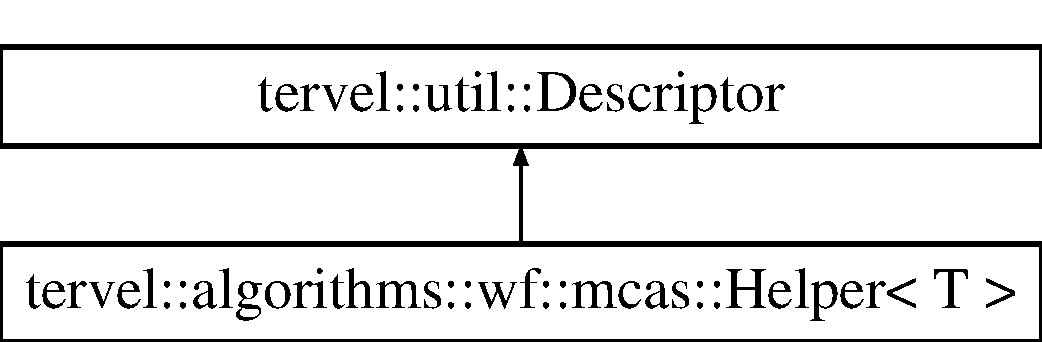
\includegraphics[height=2.000000cm]{classtervel_1_1algorithms_1_1wf_1_1mcas_1_1_helper}
\end{center}
\end{figure}
\subsection*{Public Member Functions}
\begin{DoxyCompactItemize}
\item 
\hyperlink{classtervel_1_1algorithms_1_1wf_1_1mcas_1_1_helper_adf95331e5787d82f619057cbccdf1905}{Helper} (\hyperlink{classtervel_1_1algorithms_1_1wf_1_1mcas_1_1_m_c_a_s}{M\+C\+A\+S}$<$ T $>$ $\ast$mcas\+\_\+op, \hyperlink{classtervel_1_1algorithms_1_1wf_1_1mcas_1_1_cas_row}{Cas\+Row}$<$ T $>$ $\ast$cas\+\_\+row)
\begin{DoxyCompactList}\small\item\em The \hyperlink{classtervel_1_1algorithms_1_1wf_1_1mcas_1_1_helper}{Helper} object contains a reference to the row it is associated with and the mcas operation that contains the row. \end{DoxyCompactList}\item 
bool \hyperlink{classtervel_1_1algorithms_1_1wf_1_1mcas_1_1_helper_a381449ae3b9624302008a581610f76b5}{on\+\_\+watch} (std\+::atomic$<$ void $\ast$ $>$ $\ast$address, void $\ast$value)
\begin{DoxyCompactList}\small\item\em This method is optional to implement for each sub class. \end{DoxyCompactList}\item 
void $\ast$ \hyperlink{classtervel_1_1algorithms_1_1wf_1_1mcas_1_1_helper_a952a74178febcf25e6f3fe6d3fd8f691}{complete} (void $\ast$value, std\+::atomic$<$ void $\ast$ $>$ $\ast$address)
\begin{DoxyCompactList}\small\item\em This method is implemented by each sub class and must guarantee that upon return that the descriptor no longer exists at the address it was placed. \end{DoxyCompactList}\item 
void $\ast$ \hyperlink{classtervel_1_1algorithms_1_1wf_1_1mcas_1_1_helper_ad7fbc9ead7553cb023b0ecec2eaf45d4}{get\+\_\+logical\+\_\+value} ()
\begin{DoxyCompactList}\small\item\em This method is implemented by each sub class. \end{DoxyCompactList}\end{DoxyCompactItemize}
\subsection*{Private Attributes}
\begin{DoxyCompactItemize}
\item 
\hyperlink{classtervel_1_1algorithms_1_1wf_1_1mcas_1_1_cas_row}{Cas\+Row}$<$ T $>$ $\ast$ \hyperlink{classtervel_1_1algorithms_1_1wf_1_1mcas_1_1_helper_a1dc09a369e400a1d0dc37e505b585932}{cas\+\_\+row\+\_\+}
\item 
\hyperlink{classtervel_1_1algorithms_1_1wf_1_1mcas_1_1_m_c_a_s}{M\+C\+A\+S}$<$ T $>$ $\ast$ \hyperlink{classtervel_1_1algorithms_1_1wf_1_1mcas_1_1_helper_a50a2eb6601553b9110c408f7981b7f15}{mcas\+\_\+op\+\_\+}
\end{DoxyCompactItemize}


\subsection{Detailed Description}
\subsubsection*{template$<$class T$>$class tervel\+::algorithms\+::wf\+::mcas\+::\+Helper$<$ T $>$}

This class is the \hyperlink{classtervel_1_1algorithms_1_1wf_1_1mcas_1_1_m_c_a_s}{M\+C\+A\+S} operation\textquotesingle{}s helper. 

The \hyperlink{classtervel_1_1algorithms_1_1wf_1_1mcas_1_1_helper}{Helper} or M\+C\+H is used to replace the expected value of the specified address. 

\subsection{Constructor \& Destructor Documentation}
\hypertarget{classtervel_1_1algorithms_1_1wf_1_1mcas_1_1_helper_adf95331e5787d82f619057cbccdf1905}{}\index{tervel\+::algorithms\+::wf\+::mcas\+::\+Helper@{tervel\+::algorithms\+::wf\+::mcas\+::\+Helper}!Helper@{Helper}}
\index{Helper@{Helper}!tervel\+::algorithms\+::wf\+::mcas\+::\+Helper@{tervel\+::algorithms\+::wf\+::mcas\+::\+Helper}}
\subsubsection[{Helper(\+M\+C\+A\+S$<$ T $>$ $\ast$mcas\+\_\+op, Cas\+Row$<$ T $>$ $\ast$cas\+\_\+row)}]{\setlength{\rightskip}{0pt plus 5cm}template$<$class T$>$ {\bf tervel\+::algorithms\+::wf\+::mcas\+::\+Helper}$<$ T $>$\+::{\bf Helper} (
\begin{DoxyParamCaption}
\item[{{\bf M\+C\+A\+S}$<$ T $>$ $\ast$}]{mcas\+\_\+op, }
\item[{{\bf Cas\+Row}$<$ T $>$ $\ast$}]{cas\+\_\+row}
\end{DoxyParamCaption}
)\hspace{0.3cm}{\ttfamily [inline]}}\label{classtervel_1_1algorithms_1_1wf_1_1mcas_1_1_helper_adf95331e5787d82f619057cbccdf1905}


The \hyperlink{classtervel_1_1algorithms_1_1wf_1_1mcas_1_1_helper}{Helper} object contains a reference to the row it is associated with and the mcas operation that contains the row. 


\begin{DoxyParams}{Parameters}
{\em mcas\+\_\+op} & the M\+C\+A\+S$<$\+T$>$ which contains the referenced cas\+\_\+row \\
\hline
{\em cas\+\_\+row} & the referenced row in the M\+C\+A\+S$<$\+T$>$. \\
\hline
\end{DoxyParams}


\subsection{Member Function Documentation}
\hypertarget{classtervel_1_1algorithms_1_1wf_1_1mcas_1_1_helper_a952a74178febcf25e6f3fe6d3fd8f691}{}\index{tervel\+::algorithms\+::wf\+::mcas\+::\+Helper@{tervel\+::algorithms\+::wf\+::mcas\+::\+Helper}!complete@{complete}}
\index{complete@{complete}!tervel\+::algorithms\+::wf\+::mcas\+::\+Helper@{tervel\+::algorithms\+::wf\+::mcas\+::\+Helper}}
\subsubsection[{complete(void $\ast$value, std\+::atomic$<$ void $\ast$ $>$ $\ast$address)}]{\setlength{\rightskip}{0pt plus 5cm}template$<$class T$>$ void$\ast$ {\bf tervel\+::algorithms\+::wf\+::mcas\+::\+Helper}$<$ T $>$\+::complete (
\begin{DoxyParamCaption}
\item[{void $\ast$}]{current, }
\item[{std\+::atomic$<$ void $\ast$ $>$ $\ast$}]{address}
\end{DoxyParamCaption}
)\hspace{0.3cm}{\ttfamily [inline]}, {\ttfamily [virtual]}}\label{classtervel_1_1algorithms_1_1wf_1_1mcas_1_1_helper_a952a74178febcf25e6f3fe6d3fd8f691}


This method is implemented by each sub class and must guarantee that upon return that the descriptor no longer exists at the address it was placed. 


\begin{DoxyParams}{Parameters}
{\em current} & the reference to this object as it is at the address, \\
\hline
{\em address} & the location this object was read from \\
\hline
\end{DoxyParams}


Implements \hyperlink{classtervel_1_1util_1_1_descriptor_a4303b2a08e3ab67de5533cfb20db87c9}{tervel\+::util\+::\+Descriptor}.

\hypertarget{classtervel_1_1algorithms_1_1wf_1_1mcas_1_1_helper_ad7fbc9ead7553cb023b0ecec2eaf45d4}{}\index{tervel\+::algorithms\+::wf\+::mcas\+::\+Helper@{tervel\+::algorithms\+::wf\+::mcas\+::\+Helper}!get\+\_\+logical\+\_\+value@{get\+\_\+logical\+\_\+value}}
\index{get\+\_\+logical\+\_\+value@{get\+\_\+logical\+\_\+value}!tervel\+::algorithms\+::wf\+::mcas\+::\+Helper@{tervel\+::algorithms\+::wf\+::mcas\+::\+Helper}}
\subsubsection[{get\+\_\+logical\+\_\+value()}]{\setlength{\rightskip}{0pt plus 5cm}template$<$class T$>$ void$\ast$ {\bf tervel\+::algorithms\+::wf\+::mcas\+::\+Helper}$<$ T $>$\+::get\+\_\+logical\+\_\+value (
\begin{DoxyParamCaption}
{}
\end{DoxyParamCaption}
)\hspace{0.3cm}{\ttfamily [inline]}, {\ttfamily [virtual]}}\label{classtervel_1_1algorithms_1_1wf_1_1mcas_1_1_helper_ad7fbc9ead7553cb023b0ecec2eaf45d4}


This method is implemented by each sub class. 

It returns the logical value of the past address. If the associated operation is still in progress then it will generally return the value that was replaced by this descriptor. Otherwise it will generally return the result of the operation for the specified address.

It can only be called from the static function which protects the object from being reused during the function. 

Implements \hyperlink{classtervel_1_1util_1_1_descriptor_a5b443eeb6acf1207f27a6d06c39d4ad4}{tervel\+::util\+::\+Descriptor}.

\hypertarget{classtervel_1_1algorithms_1_1wf_1_1mcas_1_1_helper_a381449ae3b9624302008a581610f76b5}{}\index{tervel\+::algorithms\+::wf\+::mcas\+::\+Helper@{tervel\+::algorithms\+::wf\+::mcas\+::\+Helper}!on\+\_\+watch@{on\+\_\+watch}}
\index{on\+\_\+watch@{on\+\_\+watch}!tervel\+::algorithms\+::wf\+::mcas\+::\+Helper@{tervel\+::algorithms\+::wf\+::mcas\+::\+Helper}}
\subsubsection[{on\+\_\+watch(std\+::atomic$<$ void $\ast$ $>$ $\ast$address, void $\ast$value)}]{\setlength{\rightskip}{0pt plus 5cm}template$<$class T$>$ bool {\bf tervel\+::algorithms\+::wf\+::mcas\+::\+Helper}$<$ T $>$\+::on\+\_\+watch (
\begin{DoxyParamCaption}
\item[{std\+::atomic$<$ void $\ast$ $>$ $\ast$}]{, }
\item[{void $\ast$}]{}
\end{DoxyParamCaption}
)\hspace{0.3cm}{\ttfamily [inline]}, {\ttfamily [virtual]}}\label{classtervel_1_1algorithms_1_1wf_1_1mcas_1_1_helper_a381449ae3b9624302008a581610f76b5}


This method is optional to implement for each sub class. 

In the event there is a complex dependency between descriptor objects, where watching one implies performing other actions, such as watching a parent object, a developer will implement this function to encapsulate that logic

This function is called by the static watch function It should not watch itself.


\begin{DoxyParams}{Parameters}
{\em address} & The location to check. \\
\hline
{\em expected} & The expected value for that location\\
\hline
\end{DoxyParams}
\begin{DoxyReturn}{Returns}
true if successful, false otherwise 
\end{DoxyReturn}


Reimplemented from \hyperlink{classtervel_1_1util_1_1_descriptor_ab643e09f20f35149dc820766b0f9ccdb}{tervel\+::util\+::\+Descriptor}.



\subsection{Member Data Documentation}
\hypertarget{classtervel_1_1algorithms_1_1wf_1_1mcas_1_1_helper_a1dc09a369e400a1d0dc37e505b585932}{}\index{tervel\+::algorithms\+::wf\+::mcas\+::\+Helper@{tervel\+::algorithms\+::wf\+::mcas\+::\+Helper}!cas\+\_\+row\+\_\+@{cas\+\_\+row\+\_\+}}
\index{cas\+\_\+row\+\_\+@{cas\+\_\+row\+\_\+}!tervel\+::algorithms\+::wf\+::mcas\+::\+Helper@{tervel\+::algorithms\+::wf\+::mcas\+::\+Helper}}
\subsubsection[{cas\+\_\+row\+\_\+}]{\setlength{\rightskip}{0pt plus 5cm}template$<$class T$>$ {\bf Cas\+Row}$<$T$>$$\ast$ {\bf tervel\+::algorithms\+::wf\+::mcas\+::\+Helper}$<$ T $>$\+::cas\+\_\+row\+\_\+\hspace{0.3cm}{\ttfamily [private]}}\label{classtervel_1_1algorithms_1_1wf_1_1mcas_1_1_helper_a1dc09a369e400a1d0dc37e505b585932}
\hypertarget{classtervel_1_1algorithms_1_1wf_1_1mcas_1_1_helper_a50a2eb6601553b9110c408f7981b7f15}{}\index{tervel\+::algorithms\+::wf\+::mcas\+::\+Helper@{tervel\+::algorithms\+::wf\+::mcas\+::\+Helper}!mcas\+\_\+op\+\_\+@{mcas\+\_\+op\+\_\+}}
\index{mcas\+\_\+op\+\_\+@{mcas\+\_\+op\+\_\+}!tervel\+::algorithms\+::wf\+::mcas\+::\+Helper@{tervel\+::algorithms\+::wf\+::mcas\+::\+Helper}}
\subsubsection[{mcas\+\_\+op\+\_\+}]{\setlength{\rightskip}{0pt plus 5cm}template$<$class T$>$ {\bf M\+C\+A\+S}$<$T$>$$\ast$ {\bf tervel\+::algorithms\+::wf\+::mcas\+::\+Helper}$<$ T $>$\+::mcas\+\_\+op\+\_\+\hspace{0.3cm}{\ttfamily [private]}}\label{classtervel_1_1algorithms_1_1wf_1_1mcas_1_1_helper_a50a2eb6601553b9110c408f7981b7f15}


The documentation for this class was generated from the following files\+:\begin{DoxyCompactItemize}
\item 
tervel/algorithms/wf/mcas/\hyperlink{mcas__casrow_8h}{mcas\+\_\+casrow.\+h}\item 
tervel/algorithms/wf/mcas/\hyperlink{mcas__helper_8h}{mcas\+\_\+helper.\+h}\end{DoxyCompactItemize}

\hypertarget{classtervel_1_1containers_1_1wf_1_1_ring_buffer_1_1_helper}{}\section{tervel\+:\+:containers\+:\+:wf\+:\+:Ring\+Buffer$<$ T $>$\+:\+:Helper$<$ T $>$ Class Template Reference}
\label{classtervel_1_1containers_1_1wf_1_1_ring_buffer_1_1_helper}\index{tervel\+::containers\+::wf\+::\+Ring\+Buffer$<$ T $>$\+::\+Helper$<$ T $>$@{tervel\+::containers\+::wf\+::\+Ring\+Buffer$<$ T $>$\+::\+Helper$<$ T $>$}}


{\ttfamily \#include $<$helper.\+h$>$}

Inheritance diagram for tervel\+:\+:containers\+:\+:wf\+:\+:Ring\+Buffer$<$ T $>$\+:\+:Helper$<$ T $>$\+:\begin{figure}[H]
\begin{center}
\leavevmode
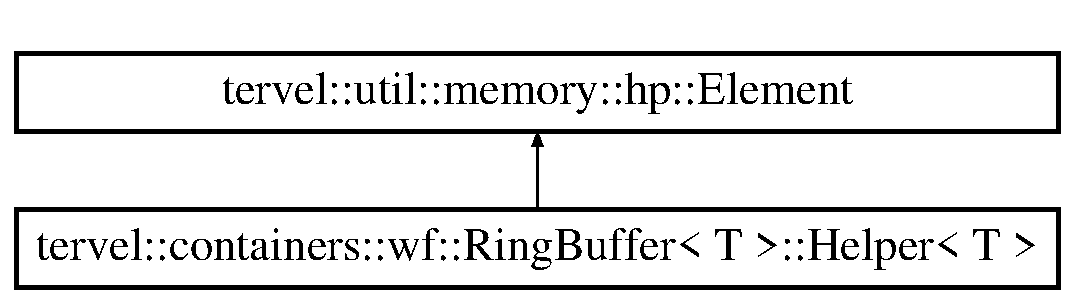
\includegraphics[height=2.000000cm]{classtervel_1_1containers_1_1wf_1_1_ring_buffer_1_1_helper}
\end{center}
\end{figure}
\subsection*{Public Member Functions}
\begin{DoxyCompactItemize}
\item 
\hyperlink{classtervel_1_1containers_1_1wf_1_1_ring_buffer_1_1_helper_a727b15617f6bd482ae200aad29e9a062}{Helper} (\hyperlink{classtervel_1_1containers_1_1wf_1_1_ring_buffer_1_1_buffer_op}{Buffer\+Op} $\ast$op, uintptr\+\_\+t old\+\_\+value)
\item 
\hyperlink{classtervel_1_1containers_1_1wf_1_1_ring_buffer_1_1_helper_a27ab01a87150b6b3561485fbb48f1a2d}{$\sim$\+Helper} ()
\item 
bool \hyperlink{classtervel_1_1containers_1_1wf_1_1_ring_buffer_1_1_helper_a2602ee377d46b4b086c5df431b851645}{on\+\_\+watch} (std\+::atomic$<$ void $\ast$ $>$ $\ast$address, void $\ast$expected)
\begin{DoxyCompactList}\small\item\em This function is used to achieve a strong watch on an Element. \end{DoxyCompactList}\item 
void $\ast$ \hyperlink{classtervel_1_1containers_1_1wf_1_1_ring_buffer_1_1_helper_ad9e59b7233276f595218f0731eb61602}{associate} ()
\item 
bool \hyperlink{classtervel_1_1containers_1_1wf_1_1_ring_buffer_1_1_helper_a82987e8211ac1e29b9f08edcee4b17e6}{valid} ()
\end{DoxyCompactItemize}
\subsection*{Static Public Member Functions}
\begin{DoxyCompactItemize}
\item 
static uintptr\+\_\+t \hyperlink{classtervel_1_1containers_1_1wf_1_1_ring_buffer_1_1_helper_ae04b46af093b7546aa05a9ce7a8533a9}{Helper\+Type} (\hyperlink{classtervel_1_1containers_1_1wf_1_1_ring_buffer_1_1_helper}{Helper} $\ast$h)
\begin{DoxyCompactList}\small\item\em Returns a uintptr\+\_\+t for the passed helper object. \end{DoxyCompactList}\item 
static bool \hyperlink{classtervel_1_1containers_1_1wf_1_1_ring_buffer_1_1_helper_aa375dafb087de1a4b6ad9d2164f390ea}{is\+Helper\+Type} (uintptr\+\_\+t val)
\item 
static \hyperlink{classtervel_1_1containers_1_1wf_1_1_ring_buffer_1_1_helper}{Helper} $\ast$ \hyperlink{classtervel_1_1containers_1_1wf_1_1_ring_buffer_1_1_helper_a4a392baf1637042a60e743b306b9399f}{get\+Helper\+Type} (uintptr\+\_\+t val)
\end{DoxyCompactItemize}
\subsection*{Public Attributes}
\begin{DoxyCompactItemize}
\item 
\hyperlink{classtervel_1_1containers_1_1wf_1_1_ring_buffer_1_1_buffer_op}{Buffer\+Op} $\ast$ \hyperlink{classtervel_1_1containers_1_1wf_1_1_ring_buffer_1_1_helper_acdb1064476d7cbc7cc18492aa2a2d9ea}{op\+\_\+}
\item 
const uintptr\+\_\+t \hyperlink{classtervel_1_1containers_1_1wf_1_1_ring_buffer_1_1_helper_a9669431287884c83f20afb6c16446a6c}{old\+\_\+value\+\_\+}
\end{DoxyCompactItemize}


\subsection{Constructor \& Destructor Documentation}
\hypertarget{classtervel_1_1containers_1_1wf_1_1_ring_buffer_1_1_helper_a727b15617f6bd482ae200aad29e9a062}{}\index{tervel\+::containers\+::wf\+::\+Ring\+Buffer\+::\+Helper@{tervel\+::containers\+::wf\+::\+Ring\+Buffer\+::\+Helper}!Helper@{Helper}}
\index{Helper@{Helper}!tervel\+::containers\+::wf\+::\+Ring\+Buffer\+::\+Helper@{tervel\+::containers\+::wf\+::\+Ring\+Buffer\+::\+Helper}}
\subsubsection[{Helper(\+Buffer\+Op $\ast$op, uintptr\+\_\+t old\+\_\+value)}]{\setlength{\rightskip}{0pt plus 5cm}template$<$typename T$>$ template$<$typename T $>$ {\bf tervel\+::containers\+::wf\+::\+Ring\+Buffer}$<$ T $>$\+::{\bf Helper}$<$ T $>$\+::{\bf Helper} (
\begin{DoxyParamCaption}
\item[{{\bf Buffer\+Op} $\ast$}]{op, }
\item[{uintptr\+\_\+t}]{old\+\_\+value}
\end{DoxyParamCaption}
)\hspace{0.3cm}{\ttfamily [inline]}}\label{classtervel_1_1containers_1_1wf_1_1_ring_buffer_1_1_helper_a727b15617f6bd482ae200aad29e9a062}
\hypertarget{classtervel_1_1containers_1_1wf_1_1_ring_buffer_1_1_helper_a27ab01a87150b6b3561485fbb48f1a2d}{}\index{tervel\+::containers\+::wf\+::\+Ring\+Buffer\+::\+Helper@{tervel\+::containers\+::wf\+::\+Ring\+Buffer\+::\+Helper}!````~Helper@{$\sim$\+Helper}}
\index{````~Helper@{$\sim$\+Helper}!tervel\+::containers\+::wf\+::\+Ring\+Buffer\+::\+Helper@{tervel\+::containers\+::wf\+::\+Ring\+Buffer\+::\+Helper}}
\subsubsection[{$\sim$\+Helper()}]{\setlength{\rightskip}{0pt plus 5cm}template$<$typename T$>$ template$<$typename T $>$ {\bf tervel\+::containers\+::wf\+::\+Ring\+Buffer}$<$ T $>$\+::{\bf Helper}$<$ T $>$\+::$\sim${\bf Helper} (
\begin{DoxyParamCaption}
{}
\end{DoxyParamCaption}
)\hspace{0.3cm}{\ttfamily [inline]}}\label{classtervel_1_1containers_1_1wf_1_1_ring_buffer_1_1_helper_a27ab01a87150b6b3561485fbb48f1a2d}


\subsection{Member Function Documentation}
\hypertarget{classtervel_1_1containers_1_1wf_1_1_ring_buffer_1_1_helper_ad9e59b7233276f595218f0731eb61602}{}\index{tervel\+::containers\+::wf\+::\+Ring\+Buffer\+::\+Helper@{tervel\+::containers\+::wf\+::\+Ring\+Buffer\+::\+Helper}!associate@{associate}}
\index{associate@{associate}!tervel\+::containers\+::wf\+::\+Ring\+Buffer\+::\+Helper@{tervel\+::containers\+::wf\+::\+Ring\+Buffer\+::\+Helper}}
\subsubsection[{associate()}]{\setlength{\rightskip}{0pt plus 5cm}template$<$typename T$>$ template$<$typename T $>$ void $\ast$ {\bf tervel\+::containers\+::wf\+::\+Ring\+Buffer}$<$ T $>$\+::{\bf Helper}$<$ T $>$\+::associate (
\begin{DoxyParamCaption}
{}
\end{DoxyParamCaption}
)}\label{classtervel_1_1containers_1_1wf_1_1_ring_buffer_1_1_helper_ad9e59b7233276f595218f0731eb61602}
\hypertarget{classtervel_1_1containers_1_1wf_1_1_ring_buffer_1_1_helper_a4a392baf1637042a60e743b306b9399f}{}\index{tervel\+::containers\+::wf\+::\+Ring\+Buffer\+::\+Helper@{tervel\+::containers\+::wf\+::\+Ring\+Buffer\+::\+Helper}!get\+Helper\+Type@{get\+Helper\+Type}}
\index{get\+Helper\+Type@{get\+Helper\+Type}!tervel\+::containers\+::wf\+::\+Ring\+Buffer\+::\+Helper@{tervel\+::containers\+::wf\+::\+Ring\+Buffer\+::\+Helper}}
\subsubsection[{get\+Helper\+Type(uintptr\+\_\+t val)}]{\setlength{\rightskip}{0pt plus 5cm}template$<$typename T$>$ template$<$typename T $>$ {\bf Ring\+Buffer}$<$ T $>$\+::{\bf Helper} $\ast$ {\bf tervel\+::containers\+::wf\+::\+Ring\+Buffer}$<$ T $>$\+::{\bf Helper}$<$ T $>$\+::get\+Helper\+Type (
\begin{DoxyParamCaption}
\item[{uintptr\+\_\+t}]{val}
\end{DoxyParamCaption}
)\hspace{0.3cm}{\ttfamily [inline]}, {\ttfamily [static]}}\label{classtervel_1_1containers_1_1wf_1_1_ring_buffer_1_1_helper_a4a392baf1637042a60e743b306b9399f}
\hypertarget{classtervel_1_1containers_1_1wf_1_1_ring_buffer_1_1_helper_ae04b46af093b7546aa05a9ce7a8533a9}{}\index{tervel\+::containers\+::wf\+::\+Ring\+Buffer\+::\+Helper@{tervel\+::containers\+::wf\+::\+Ring\+Buffer\+::\+Helper}!Helper\+Type@{Helper\+Type}}
\index{Helper\+Type@{Helper\+Type}!tervel\+::containers\+::wf\+::\+Ring\+Buffer\+::\+Helper@{tervel\+::containers\+::wf\+::\+Ring\+Buffer\+::\+Helper}}
\subsubsection[{Helper\+Type(\+Helper $\ast$h)}]{\setlength{\rightskip}{0pt plus 5cm}template$<$typename T$>$ template$<$typename T $>$ uintptr\+\_\+t {\bf tervel\+::containers\+::wf\+::\+Ring\+Buffer}$<$ T $>$\+::{\bf Helper}$<$ T $>$\+::Helper\+Type (
\begin{DoxyParamCaption}
\item[{{\bf Helper}$<$ T $>$ $\ast$}]{h}
\end{DoxyParamCaption}
)\hspace{0.3cm}{\ttfamily [inline]}, {\ttfamily [static]}}\label{classtervel_1_1containers_1_1wf_1_1_ring_buffer_1_1_helper_ae04b46af093b7546aa05a9ce7a8533a9}


Returns a uintptr\+\_\+t for the passed helper object. 

Returns a uintptr\+\_\+t for the passed helper object by performing a bitwise O\+R with h and oprec\+\_\+lsb


\begin{DoxyParams}{Parameters}
{\em h} & the pointer to O\+R \\
\hline
\end{DoxyParams}
\begin{DoxyReturn}{Returns}
the result of the bitwise or. 
\end{DoxyReturn}
\hypertarget{classtervel_1_1containers_1_1wf_1_1_ring_buffer_1_1_helper_aa375dafb087de1a4b6ad9d2164f390ea}{}\index{tervel\+::containers\+::wf\+::\+Ring\+Buffer\+::\+Helper@{tervel\+::containers\+::wf\+::\+Ring\+Buffer\+::\+Helper}!is\+Helper\+Type@{is\+Helper\+Type}}
\index{is\+Helper\+Type@{is\+Helper\+Type}!tervel\+::containers\+::wf\+::\+Ring\+Buffer\+::\+Helper@{tervel\+::containers\+::wf\+::\+Ring\+Buffer\+::\+Helper}}
\subsubsection[{is\+Helper\+Type(uintptr\+\_\+t val)}]{\setlength{\rightskip}{0pt plus 5cm}template$<$typename T$>$ template$<$typename T $>$ bool {\bf tervel\+::containers\+::wf\+::\+Ring\+Buffer}$<$ T $>$\+::{\bf Helper}$<$ T $>$\+::is\+Helper\+Type (
\begin{DoxyParamCaption}
\item[{uintptr\+\_\+t}]{val}
\end{DoxyParamCaption}
)\hspace{0.3cm}{\ttfamily [inline]}, {\ttfamily [static]}}\label{classtervel_1_1containers_1_1wf_1_1_ring_buffer_1_1_helper_aa375dafb087de1a4b6ad9d2164f390ea}
\hypertarget{classtervel_1_1containers_1_1wf_1_1_ring_buffer_1_1_helper_a2602ee377d46b4b086c5df431b851645}{}\index{tervel\+::containers\+::wf\+::\+Ring\+Buffer\+::\+Helper@{tervel\+::containers\+::wf\+::\+Ring\+Buffer\+::\+Helper}!on\+\_\+watch@{on\+\_\+watch}}
\index{on\+\_\+watch@{on\+\_\+watch}!tervel\+::containers\+::wf\+::\+Ring\+Buffer\+::\+Helper@{tervel\+::containers\+::wf\+::\+Ring\+Buffer\+::\+Helper}}
\subsubsection[{on\+\_\+watch(std\+::atomic$<$ void $\ast$ $>$ $\ast$address, void $\ast$expected)}]{\setlength{\rightskip}{0pt plus 5cm}template$<$typename T$>$ template$<$typename T $>$ bool {\bf tervel\+::containers\+::wf\+::\+Ring\+Buffer}$<$ T $>$\+::{\bf Helper}$<$ T $>$\+::on\+\_\+watch (
\begin{DoxyParamCaption}
\item[{std\+::atomic$<$ void $\ast$ $>$ $\ast$}]{address, }
\item[{void $\ast$}]{expected}
\end{DoxyParamCaption}
)\hspace{0.3cm}{\ttfamily [virtual]}}\label{classtervel_1_1containers_1_1wf_1_1_ring_buffer_1_1_helper_a2602ee377d46b4b086c5df431b851645}


This function is used to achieve a strong watch on an Element. 

Classes wishing to express this should override this function.


\begin{DoxyParams}{Parameters}
{\em address} & the expected was load from \\
\hline
{\em expected} & the last known value of address \\
\hline
\end{DoxyParams}
\begin{DoxyReturn}{Returns}
whether or not the element was succefully watched. 
\end{DoxyReturn}


Reimplemented from \hyperlink{classtervel_1_1util_1_1memory_1_1hp_1_1_element_a53493ef4754dd77016139863af964f90}{tervel\+::util\+::memory\+::hp\+::\+Element}.

\hypertarget{classtervel_1_1containers_1_1wf_1_1_ring_buffer_1_1_helper_a82987e8211ac1e29b9f08edcee4b17e6}{}\index{tervel\+::containers\+::wf\+::\+Ring\+Buffer\+::\+Helper@{tervel\+::containers\+::wf\+::\+Ring\+Buffer\+::\+Helper}!valid@{valid}}
\index{valid@{valid}!tervel\+::containers\+::wf\+::\+Ring\+Buffer\+::\+Helper@{tervel\+::containers\+::wf\+::\+Ring\+Buffer\+::\+Helper}}
\subsubsection[{valid()}]{\setlength{\rightskip}{0pt plus 5cm}template$<$typename T$>$ template$<$typename T $>$ bool {\bf tervel\+::containers\+::wf\+::\+Ring\+Buffer}$<$ T $>$\+::{\bf Helper}$<$ T $>$\+::valid (
\begin{DoxyParamCaption}
{}
\end{DoxyParamCaption}
)}\label{classtervel_1_1containers_1_1wf_1_1_ring_buffer_1_1_helper_a82987e8211ac1e29b9f08edcee4b17e6}


\subsection{Member Data Documentation}
\hypertarget{classtervel_1_1containers_1_1wf_1_1_ring_buffer_1_1_helper_a9669431287884c83f20afb6c16446a6c}{}\index{tervel\+::containers\+::wf\+::\+Ring\+Buffer\+::\+Helper@{tervel\+::containers\+::wf\+::\+Ring\+Buffer\+::\+Helper}!old\+\_\+value\+\_\+@{old\+\_\+value\+\_\+}}
\index{old\+\_\+value\+\_\+@{old\+\_\+value\+\_\+}!tervel\+::containers\+::wf\+::\+Ring\+Buffer\+::\+Helper@{tervel\+::containers\+::wf\+::\+Ring\+Buffer\+::\+Helper}}
\subsubsection[{old\+\_\+value\+\_\+}]{\setlength{\rightskip}{0pt plus 5cm}template$<$typename T$>$ template$<$typename T $>$ const uintptr\+\_\+t {\bf tervel\+::containers\+::wf\+::\+Ring\+Buffer}$<$ T $>$\+::{\bf Helper}$<$ T $>$\+::old\+\_\+value\+\_\+}\label{classtervel_1_1containers_1_1wf_1_1_ring_buffer_1_1_helper_a9669431287884c83f20afb6c16446a6c}
\hypertarget{classtervel_1_1containers_1_1wf_1_1_ring_buffer_1_1_helper_acdb1064476d7cbc7cc18492aa2a2d9ea}{}\index{tervel\+::containers\+::wf\+::\+Ring\+Buffer\+::\+Helper@{tervel\+::containers\+::wf\+::\+Ring\+Buffer\+::\+Helper}!op\+\_\+@{op\+\_\+}}
\index{op\+\_\+@{op\+\_\+}!tervel\+::containers\+::wf\+::\+Ring\+Buffer\+::\+Helper@{tervel\+::containers\+::wf\+::\+Ring\+Buffer\+::\+Helper}}
\subsubsection[{op\+\_\+}]{\setlength{\rightskip}{0pt plus 5cm}template$<$typename T$>$ template$<$typename T $>$ {\bf Buffer\+Op}$\ast$ {\bf tervel\+::containers\+::wf\+::\+Ring\+Buffer}$<$ T $>$\+::{\bf Helper}$<$ T $>$\+::op\+\_\+}\label{classtervel_1_1containers_1_1wf_1_1_ring_buffer_1_1_helper_acdb1064476d7cbc7cc18492aa2a2d9ea}


The documentation for this class was generated from the following files\+:\begin{DoxyCompactItemize}
\item 
tervel/containers/wf/ring-\/buffer/\hyperlink{helper_8h}{helper.\+h}\item 
tervel/containers/wf/ring-\/buffer/\hyperlink{helper__imp_8h}{helper\+\_\+imp.\+h}\end{DoxyCompactItemize}

\hypertarget{class_insert_at}{}\section{Insert\+At Class Reference}
\label{class_insert_at}\index{Insert\+At@{Insert\+At}}


{\ttfamily \#include $<$insertat\+\_\+op.\+h$>$}

Inheritance diagram for Insert\+At\+:\begin{figure}[H]
\begin{center}
\leavevmode
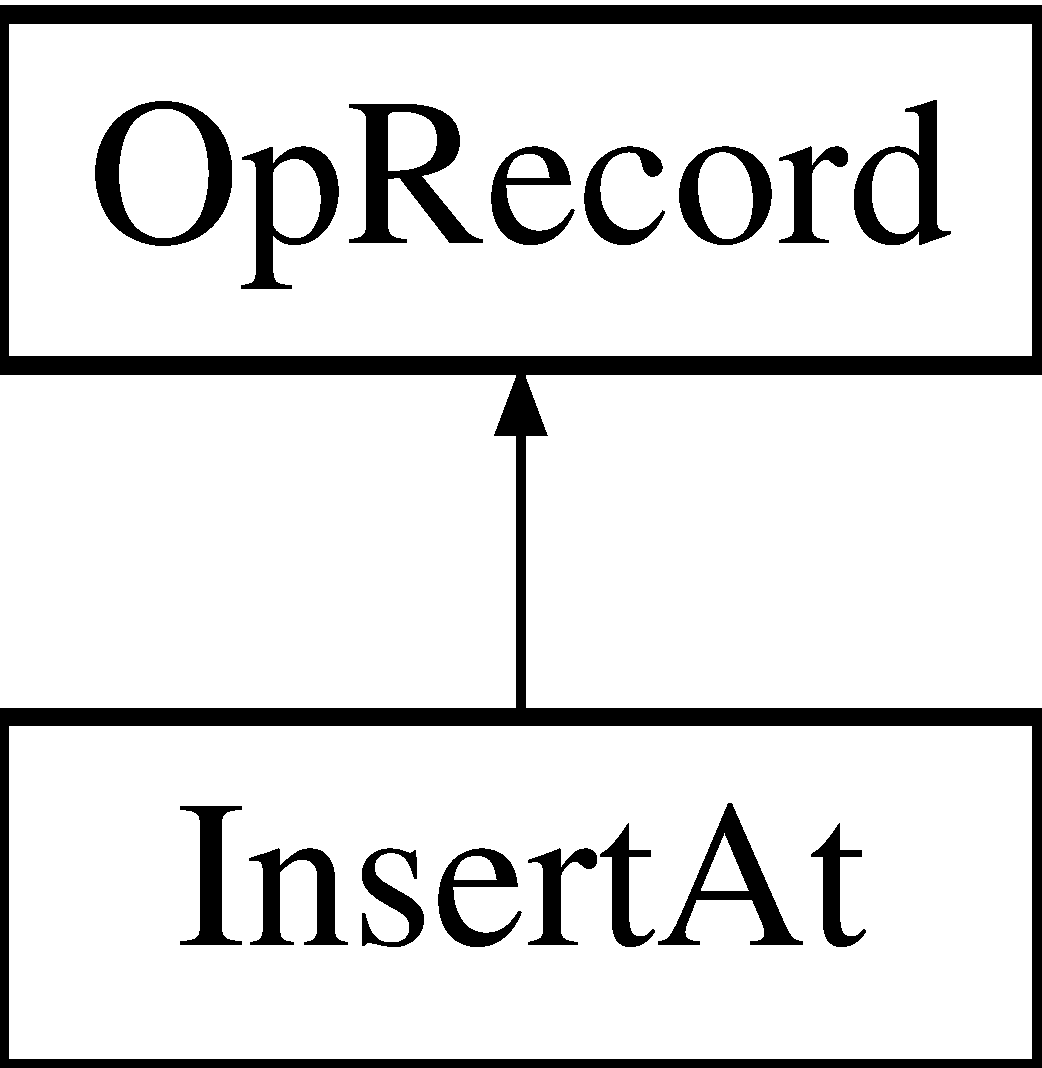
\includegraphics[height=2.000000cm]{class_insert_at}
\end{center}
\end{figure}
\subsection*{Public Member Functions}
\begin{DoxyCompactItemize}
\item 
void \hyperlink{class_insert_at_a44d47d24a48f8bcedd833129dadedea0}{init} (int p, void $\ast$v)
\item 
\hyperlink{class_insert_at_aa86ff4bb5674c3be14a46a29dacd3d9f}{Insert\+At} (int p, void $\ast$v)
\item 
void \hyperlink{class_insert_at_a80960f22e24c552a92f02963b3f9032c}{execute} (W\+F\+Vector $\ast$vec)
\item 
bool \hyperlink{class_insert_at_aca674527cd17b29b486a3082ab0437a4}{s\+\_\+execute} (W\+F\+Vector $\ast$vec)
\item 
void \hyperlink{class_insert_at_af3728e08aaa557a8c99ba81564120597}{cleanup} (W\+F\+Vector $\ast$vec, int \hyperlink{class_insert_at_a926928e16ec2ab511860662a01f3082a}{pos})
\item 
bool \hyperlink{class_insert_at_a2d95031cbed8c06477dd5001588757ca}{complete} (W\+F\+Vector $\ast$vec, int \hyperlink{class_insert_at_a926928e16ec2ab511860662a01f3082a}{pos})
\item 
bool \hyperlink{class_insert_at_a09d79636c2ba9023e3600d80d0af314c}{try\+Free} ()
\item 
void $\ast$ \hyperlink{class_insert_at_a7ccae8ef989a96aece9e7aef1afbd553}{read\+Through} (\hyperlink{class_shift_helper}{Shift\+Helper}$<$ \hyperlink{class_insert_at}{Insert\+At} $>$ $\ast$helper)
\end{DoxyCompactItemize}
\subsection*{Public Attributes}
\begin{DoxyCompactItemize}
\item 
void $\ast$ \hyperlink{class_insert_at_a4cd84946e247761597bde3791508d820}{rvalue}
\item 
int \hyperlink{class_insert_at_a926928e16ec2ab511860662a01f3082a}{pos}
\item 
std\+::atomic$<$ \hyperlink{class_shift_helper}{Shift\+Helper}$<$ \hyperlink{class_insert_at}{Insert\+At} $>$ $\ast$ $>$ \hyperlink{class_insert_at_a05c82ae139b7af1675eeaa58dd8f930a}{next}
\item 
std\+::atomic$<$ bool $>$ \hyperlink{class_insert_at_a258e77cb8a4bf7676290c28428b58d5c}{is\+Complete}
\end{DoxyCompactItemize}


\subsection{Constructor \& Destructor Documentation}
\hypertarget{class_insert_at_aa86ff4bb5674c3be14a46a29dacd3d9f}{}\index{Insert\+At@{Insert\+At}!Insert\+At@{Insert\+At}}
\index{Insert\+At@{Insert\+At}!Insert\+At@{Insert\+At}}
\subsubsection[{Insert\+At(int p, void $\ast$v)}]{\setlength{\rightskip}{0pt plus 5cm}Insert\+At\+::\+Insert\+At (
\begin{DoxyParamCaption}
\item[{int}]{p, }
\item[{void $\ast$}]{v}
\end{DoxyParamCaption}
)\hspace{0.3cm}{\ttfamily [inline]}}\label{class_insert_at_aa86ff4bb5674c3be14a46a29dacd3d9f}


\subsection{Member Function Documentation}
\hypertarget{class_insert_at_af3728e08aaa557a8c99ba81564120597}{}\index{Insert\+At@{Insert\+At}!cleanup@{cleanup}}
\index{cleanup@{cleanup}!Insert\+At@{Insert\+At}}
\subsubsection[{cleanup(\+W\+F\+Vector $\ast$vec, int pos)}]{\setlength{\rightskip}{0pt plus 5cm}void Insert\+At\+::cleanup (
\begin{DoxyParamCaption}
\item[{W\+F\+Vector $\ast$}]{vec, }
\item[{int}]{pos}
\end{DoxyParamCaption}
)}\label{class_insert_at_af3728e08aaa557a8c99ba81564120597}
\hypertarget{class_insert_at_a2d95031cbed8c06477dd5001588757ca}{}\index{Insert\+At@{Insert\+At}!complete@{complete}}
\index{complete@{complete}!Insert\+At@{Insert\+At}}
\subsubsection[{complete(\+W\+F\+Vector $\ast$vec, int pos)}]{\setlength{\rightskip}{0pt plus 5cm}bool Insert\+At\+::complete (
\begin{DoxyParamCaption}
\item[{W\+F\+Vector $\ast$}]{vec, }
\item[{int}]{pos}
\end{DoxyParamCaption}
)\hspace{0.3cm}{\ttfamily [inline]}}\label{class_insert_at_a2d95031cbed8c06477dd5001588757ca}
\hypertarget{class_insert_at_a80960f22e24c552a92f02963b3f9032c}{}\index{Insert\+At@{Insert\+At}!execute@{execute}}
\index{execute@{execute}!Insert\+At@{Insert\+At}}
\subsubsection[{execute(\+W\+F\+Vector $\ast$vec)}]{\setlength{\rightskip}{0pt plus 5cm}void Insert\+At\+::execute (
\begin{DoxyParamCaption}
\item[{W\+F\+Vector $\ast$}]{vec}
\end{DoxyParamCaption}
)\hspace{0.3cm}{\ttfamily [inline]}}\label{class_insert_at_a80960f22e24c552a92f02963b3f9032c}
\hypertarget{class_insert_at_a44d47d24a48f8bcedd833129dadedea0}{}\index{Insert\+At@{Insert\+At}!init@{init}}
\index{init@{init}!Insert\+At@{Insert\+At}}
\subsubsection[{init(int p, void $\ast$v)}]{\setlength{\rightskip}{0pt plus 5cm}void Insert\+At\+::init (
\begin{DoxyParamCaption}
\item[{int}]{p, }
\item[{void $\ast$}]{v}
\end{DoxyParamCaption}
)\hspace{0.3cm}{\ttfamily [inline]}}\label{class_insert_at_a44d47d24a48f8bcedd833129dadedea0}
\hypertarget{class_insert_at_a7ccae8ef989a96aece9e7aef1afbd553}{}\index{Insert\+At@{Insert\+At}!read\+Through@{read\+Through}}
\index{read\+Through@{read\+Through}!Insert\+At@{Insert\+At}}
\subsubsection[{read\+Through(\+Shift\+Helper$<$ Insert\+At $>$ $\ast$helper)}]{\setlength{\rightskip}{0pt plus 5cm}void $\ast$ Insert\+At\+::read\+Through (
\begin{DoxyParamCaption}
\item[{{\bf Shift\+Helper}$<$ {\bf Insert\+At} $>$ $\ast$}]{helper}
\end{DoxyParamCaption}
)}\label{class_insert_at_a7ccae8ef989a96aece9e7aef1afbd553}
\hypertarget{class_insert_at_aca674527cd17b29b486a3082ab0437a4}{}\index{Insert\+At@{Insert\+At}!s\+\_\+execute@{s\+\_\+execute}}
\index{s\+\_\+execute@{s\+\_\+execute}!Insert\+At@{Insert\+At}}
\subsubsection[{s\+\_\+execute(\+W\+F\+Vector $\ast$vec)}]{\setlength{\rightskip}{0pt plus 5cm}bool Insert\+At\+::s\+\_\+execute (
\begin{DoxyParamCaption}
\item[{W\+F\+Vector $\ast$}]{vec}
\end{DoxyParamCaption}
)\hspace{0.3cm}{\ttfamily [inline]}}\label{class_insert_at_aca674527cd17b29b486a3082ab0437a4}
\hypertarget{class_insert_at_a09d79636c2ba9023e3600d80d0af314c}{}\index{Insert\+At@{Insert\+At}!try\+Free@{try\+Free}}
\index{try\+Free@{try\+Free}!Insert\+At@{Insert\+At}}
\subsubsection[{try\+Free()}]{\setlength{\rightskip}{0pt plus 5cm}bool Insert\+At\+::try\+Free (
\begin{DoxyParamCaption}
{}
\end{DoxyParamCaption}
)}\label{class_insert_at_a09d79636c2ba9023e3600d80d0af314c}


\subsection{Member Data Documentation}
\hypertarget{class_insert_at_a258e77cb8a4bf7676290c28428b58d5c}{}\index{Insert\+At@{Insert\+At}!is\+Complete@{is\+Complete}}
\index{is\+Complete@{is\+Complete}!Insert\+At@{Insert\+At}}
\subsubsection[{is\+Complete}]{\setlength{\rightskip}{0pt plus 5cm}std\+::atomic$<$bool$>$ Insert\+At\+::is\+Complete}\label{class_insert_at_a258e77cb8a4bf7676290c28428b58d5c}
\hypertarget{class_insert_at_a05c82ae139b7af1675eeaa58dd8f930a}{}\index{Insert\+At@{Insert\+At}!next@{next}}
\index{next@{next}!Insert\+At@{Insert\+At}}
\subsubsection[{next}]{\setlength{\rightskip}{0pt plus 5cm}std\+::atomic$<${\bf Shift\+Helper}$<${\bf Insert\+At}$>$ $\ast$$>$ Insert\+At\+::next}\label{class_insert_at_a05c82ae139b7af1675eeaa58dd8f930a}
\hypertarget{class_insert_at_a926928e16ec2ab511860662a01f3082a}{}\index{Insert\+At@{Insert\+At}!pos@{pos}}
\index{pos@{pos}!Insert\+At@{Insert\+At}}
\subsubsection[{pos}]{\setlength{\rightskip}{0pt plus 5cm}int Insert\+At\+::pos}\label{class_insert_at_a926928e16ec2ab511860662a01f3082a}
\hypertarget{class_insert_at_a4cd84946e247761597bde3791508d820}{}\index{Insert\+At@{Insert\+At}!rvalue@{rvalue}}
\index{rvalue@{rvalue}!Insert\+At@{Insert\+At}}
\subsubsection[{rvalue}]{\setlength{\rightskip}{0pt plus 5cm}void$\ast$ Insert\+At\+::rvalue}\label{class_insert_at_a4cd84946e247761597bde3791508d820}


The documentation for this class was generated from the following file\+:\begin{DoxyCompactItemize}
\item 
tervel/containers/wf/vector/old/\hyperlink{insertat__op_8h}{insertat\+\_\+op.\+h}\end{DoxyCompactItemize}

\hypertarget{struct_test_class_1_1less__s}{}\section{Test\+Class$<$ Key, Value $>$\+:\+:less\+\_\+s$<$ T $>$ Struct Template Reference}
\label{struct_test_class_1_1less__s}\index{Test\+Class$<$ Key, Value $>$\+::less\+\_\+s$<$ T $>$@{Test\+Class$<$ Key, Value $>$\+::less\+\_\+s$<$ T $>$}}
Inheritance diagram for Test\+Class$<$ Key, Value $>$\+:\+:less\+\_\+s$<$ T $>$\+:\begin{figure}[H]
\begin{center}
\leavevmode
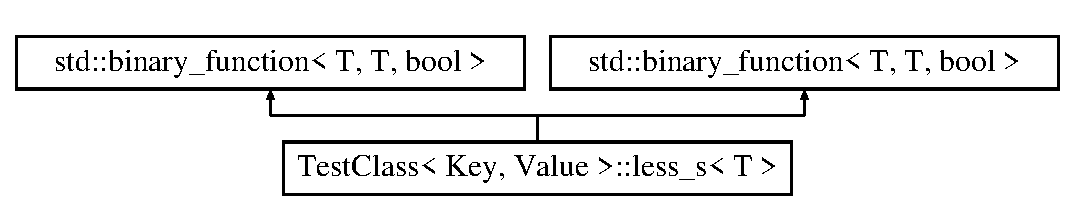
\includegraphics[height=2.000000cm]{struct_test_class_1_1less__s}
\end{center}
\end{figure}
\subsection*{Public Member Functions}
\begin{DoxyCompactItemize}
\item 
bool \hyperlink{struct_test_class_1_1less__s_a1bd896c442f180da6c02381aa4fce63e}{operator()} (const T \&x, const T \&y) const 
\item 
bool \hyperlink{struct_test_class_1_1less__s_a1bd896c442f180da6c02381aa4fce63e}{operator()} (const T \&x, const T \&y) const 
\end{DoxyCompactItemize}


\subsection{Member Function Documentation}
\hypertarget{struct_test_class_1_1less__s_a1bd896c442f180da6c02381aa4fce63e}{}\index{Test\+Class\+::less\+\_\+s@{Test\+Class\+::less\+\_\+s}!operator()@{operator()}}
\index{operator()@{operator()}!Test\+Class\+::less\+\_\+s@{Test\+Class\+::less\+\_\+s}}
\subsubsection[{operator()(const T \&x, const T \&y) const }]{\setlength{\rightskip}{0pt plus 5cm}template$<$class Key, class Value$>$ template$<$class T $>$ bool {\bf Test\+Class}$<$ Key, {\bf Value} $>$\+::{\bf less\+\_\+s}$<$ T $>$\+::operator() (
\begin{DoxyParamCaption}
\item[{const T \&}]{x, }
\item[{const T \&}]{y}
\end{DoxyParamCaption}
) const\hspace{0.3cm}{\ttfamily [inline]}}\label{struct_test_class_1_1less__s_a1bd896c442f180da6c02381aa4fce63e}
\hypertarget{struct_test_class_1_1less__s_a1bd896c442f180da6c02381aa4fce63e}{}\index{Test\+Class\+::less\+\_\+s@{Test\+Class\+::less\+\_\+s}!operator()@{operator()}}
\index{operator()@{operator()}!Test\+Class\+::less\+\_\+s@{Test\+Class\+::less\+\_\+s}}
\subsubsection[{operator()(const T \&x, const T \&y) const }]{\setlength{\rightskip}{0pt plus 5cm}template$<$class Key, class Value$>$ template$<$class T $>$ bool {\bf Test\+Class}$<$ Key, {\bf Value} $>$\+::{\bf less\+\_\+s}$<$ T $>$\+::operator() (
\begin{DoxyParamCaption}
\item[{const T \&}]{x, }
\item[{const T \&}]{y}
\end{DoxyParamCaption}
) const\hspace{0.3cm}{\ttfamily [inline]}}\label{struct_test_class_1_1less__s_a1bd896c442f180da6c02381aa4fce63e}


The documentation for this struct was generated from the following files\+:\begin{DoxyCompactItemize}
\item 
tervel/tests/hash\+\_\+map/api/\hyperlink{cds__michael__map_8h}{cds\+\_\+michael\+\_\+map.\+h}\item 
tervel/tests/hash\+\_\+map/api/\hyperlink{cds__split__map_8h}{cds\+\_\+split\+\_\+map.\+h}\end{DoxyCompactItemize}

\hypertarget{classtervel_1_1util_1_1_progress_assurance_1_1_limit}{}\section{tervel\+:\+:util\+:\+:Progress\+Assurance\+:\+:Limit Class Reference}
\label{classtervel_1_1util_1_1_progress_assurance_1_1_limit}\index{tervel\+::util\+::\+Progress\+Assurance\+::\+Limit@{tervel\+::util\+::\+Progress\+Assurance\+::\+Limit}}


{\ttfamily \#include $<$progress\+\_\+assurance.\+h$>$}

\subsection*{Public Member Functions}
\begin{DoxyCompactItemize}
\item 
\hyperlink{classtervel_1_1util_1_1_progress_assurance_1_1_limit_a01796959d367f7424ce8161e529f7232}{Limit} (size\+\_\+t limit=\hyperlink{util_8h_ad2402840ec2629b707473cbb5e0e26d7}{T\+E\+R\+V\+E\+L\+\_\+\+P\+R\+O\+G\+\_\+\+A\+S\+S\+U\+R\+\_\+\+L\+I\+M\+I\+T})
\item 
bool \hyperlink{classtervel_1_1util_1_1_progress_assurance_1_1_limit_a7734a52404e54e898f5a14b3a8979077}{is\+Delayed} (size\+\_\+t val=1)
\item 
void \hyperlink{classtervel_1_1util_1_1_progress_assurance_1_1_limit_a03a87c8697ddfb04712851114bb66e32}{reset} (size\+\_\+t limit=\hyperlink{util_8h_ad2402840ec2629b707473cbb5e0e26d7}{T\+E\+R\+V\+E\+L\+\_\+\+P\+R\+O\+G\+\_\+\+A\+S\+S\+U\+R\+\_\+\+L\+I\+M\+I\+T})
\end{DoxyCompactItemize}
\subsection*{Private Attributes}
\begin{DoxyCompactItemize}
\item 
size\+\_\+t \hyperlink{classtervel_1_1util_1_1_progress_assurance_1_1_limit_a08bd5c60326801e6337cbe1b3f184ab1}{counter\+\_\+}
\end{DoxyCompactItemize}


\subsection{Constructor \& Destructor Documentation}
\hypertarget{classtervel_1_1util_1_1_progress_assurance_1_1_limit_a01796959d367f7424ce8161e529f7232}{}\index{tervel\+::util\+::\+Progress\+Assurance\+::\+Limit@{tervel\+::util\+::\+Progress\+Assurance\+::\+Limit}!Limit@{Limit}}
\index{Limit@{Limit}!tervel\+::util\+::\+Progress\+Assurance\+::\+Limit@{tervel\+::util\+::\+Progress\+Assurance\+::\+Limit}}
\subsubsection[{Limit(size\+\_\+t limit=\+T\+E\+R\+V\+E\+L\+\_\+\+P\+R\+O\+G\+\_\+\+A\+S\+S\+U\+R\+\_\+\+L\+I\+M\+I\+T)}]{\setlength{\rightskip}{0pt plus 5cm}tervel\+::util\+::\+Progress\+Assurance\+::\+Limit\+::\+Limit (
\begin{DoxyParamCaption}
\item[{size\+\_\+t}]{limit = {\ttfamily {\bf T\+E\+R\+V\+E\+L\+\_\+\+P\+R\+O\+G\+\_\+\+A\+S\+S\+U\+R\+\_\+\+L\+I\+M\+I\+T}}}
\end{DoxyParamCaption}
)\hspace{0.3cm}{\ttfamily [inline]}, {\ttfamily [explicit]}}\label{classtervel_1_1util_1_1_progress_assurance_1_1_limit_a01796959d367f7424ce8161e529f7232}


\subsection{Member Function Documentation}
\hypertarget{classtervel_1_1util_1_1_progress_assurance_1_1_limit_a7734a52404e54e898f5a14b3a8979077}{}\index{tervel\+::util\+::\+Progress\+Assurance\+::\+Limit@{tervel\+::util\+::\+Progress\+Assurance\+::\+Limit}!is\+Delayed@{is\+Delayed}}
\index{is\+Delayed@{is\+Delayed}!tervel\+::util\+::\+Progress\+Assurance\+::\+Limit@{tervel\+::util\+::\+Progress\+Assurance\+::\+Limit}}
\subsubsection[{is\+Delayed(size\+\_\+t val=1)}]{\setlength{\rightskip}{0pt plus 5cm}bool tervel\+::util\+::\+Progress\+Assurance\+::\+Limit\+::is\+Delayed (
\begin{DoxyParamCaption}
\item[{size\+\_\+t}]{val = {\ttfamily 1}}
\end{DoxyParamCaption}
)\hspace{0.3cm}{\ttfamily [inline]}}\label{classtervel_1_1util_1_1_progress_assurance_1_1_limit_a7734a52404e54e898f5a14b3a8979077}
\hypertarget{classtervel_1_1util_1_1_progress_assurance_1_1_limit_a03a87c8697ddfb04712851114bb66e32}{}\index{tervel\+::util\+::\+Progress\+Assurance\+::\+Limit@{tervel\+::util\+::\+Progress\+Assurance\+::\+Limit}!reset@{reset}}
\index{reset@{reset}!tervel\+::util\+::\+Progress\+Assurance\+::\+Limit@{tervel\+::util\+::\+Progress\+Assurance\+::\+Limit}}
\subsubsection[{reset(size\+\_\+t limit=\+T\+E\+R\+V\+E\+L\+\_\+\+P\+R\+O\+G\+\_\+\+A\+S\+S\+U\+R\+\_\+\+L\+I\+M\+I\+T)}]{\setlength{\rightskip}{0pt plus 5cm}void tervel\+::util\+::\+Progress\+Assurance\+::\+Limit\+::reset (
\begin{DoxyParamCaption}
\item[{size\+\_\+t}]{limit = {\ttfamily {\bf T\+E\+R\+V\+E\+L\+\_\+\+P\+R\+O\+G\+\_\+\+A\+S\+S\+U\+R\+\_\+\+L\+I\+M\+I\+T}}}
\end{DoxyParamCaption}
)\hspace{0.3cm}{\ttfamily [inline]}}\label{classtervel_1_1util_1_1_progress_assurance_1_1_limit_a03a87c8697ddfb04712851114bb66e32}


\subsection{Member Data Documentation}
\hypertarget{classtervel_1_1util_1_1_progress_assurance_1_1_limit_a08bd5c60326801e6337cbe1b3f184ab1}{}\index{tervel\+::util\+::\+Progress\+Assurance\+::\+Limit@{tervel\+::util\+::\+Progress\+Assurance\+::\+Limit}!counter\+\_\+@{counter\+\_\+}}
\index{counter\+\_\+@{counter\+\_\+}!tervel\+::util\+::\+Progress\+Assurance\+::\+Limit@{tervel\+::util\+::\+Progress\+Assurance\+::\+Limit}}
\subsubsection[{counter\+\_\+}]{\setlength{\rightskip}{0pt plus 5cm}size\+\_\+t tervel\+::util\+::\+Progress\+Assurance\+::\+Limit\+::counter\+\_\+\hspace{0.3cm}{\ttfamily [private]}}\label{classtervel_1_1util_1_1_progress_assurance_1_1_limit_a08bd5c60326801e6337cbe1b3f184ab1}


The documentation for this class was generated from the following file\+:\begin{DoxyCompactItemize}
\item 
tervel/util/\hyperlink{progress__assurance_8h}{progress\+\_\+assurance.\+h}\end{DoxyCompactItemize}

\hypertarget{struct_test_class_1_1list__traits}{}\section{Test\+Class$<$ Key, Value $>$\+:\+:list\+\_\+traits Struct Reference}
\label{struct_test_class_1_1list__traits}\index{Test\+Class$<$ Key, Value $>$\+::list\+\_\+traits@{Test\+Class$<$ Key, Value $>$\+::list\+\_\+traits}}
Inheritance diagram for Test\+Class$<$ Key, Value $>$\+:\+:list\+\_\+traits\+:\begin{figure}[H]
\begin{center}
\leavevmode
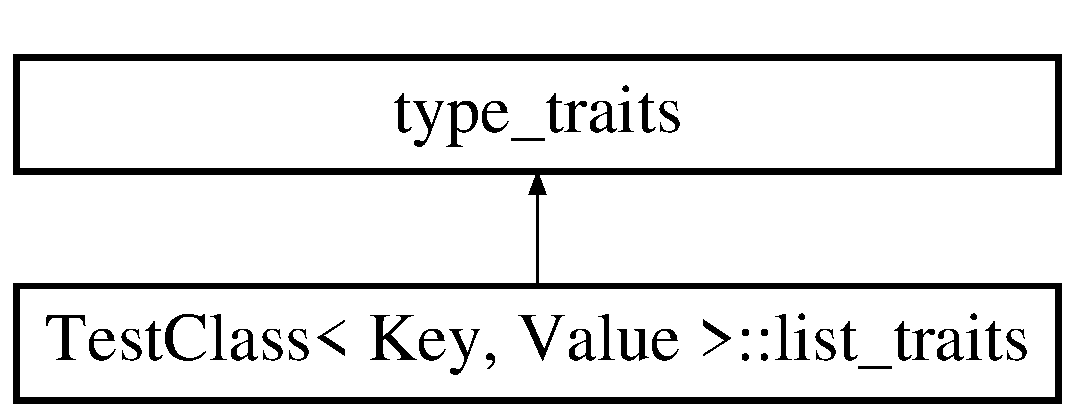
\includegraphics[height=2.000000cm]{struct_test_class_1_1list__traits}
\end{center}
\end{figure}
\subsection*{Public Types}
\begin{DoxyCompactItemize}
\item 
typedef struct \hyperlink{struct_test_class_1_1less__s}{less\+\_\+s}$<$ Key $>$ \hyperlink{struct_test_class_1_1list__traits_ae7d3e41718101d189b822e03a4cbb56b}{less}
\end{DoxyCompactItemize}


\subsection{Member Typedef Documentation}
\hypertarget{struct_test_class_1_1list__traits_ae7d3e41718101d189b822e03a4cbb56b}{}\index{Test\+Class\+::list\+\_\+traits@{Test\+Class\+::list\+\_\+traits}!less@{less}}
\index{less@{less}!Test\+Class\+::list\+\_\+traits@{Test\+Class\+::list\+\_\+traits}}
\subsubsection[{less}]{\setlength{\rightskip}{0pt plus 5cm}template$<$class Key, class Value$>$ typedef struct {\bf less\+\_\+s}$<$ Key $>$ {\bf Test\+Class}$<$ Key, {\bf Value} $>$\+::{\bf list\+\_\+traits\+::less}}\label{struct_test_class_1_1list__traits_ae7d3e41718101d189b822e03a4cbb56b}


The documentation for this struct was generated from the following file\+:\begin{DoxyCompactItemize}
\item 
tervel/tests/hash\+\_\+map/api/\hyperlink{cds__michael__map_8h}{cds\+\_\+michael\+\_\+map.\+h}\end{DoxyCompactItemize}

\hypertarget{classtervel_1_1util_1_1memory_1_1hp_1_1_list_manager}{}\section{tervel\+:\+:util\+:\+:memory\+:\+:hp\+:\+:List\+Manager Class Reference}
\label{classtervel_1_1util_1_1memory_1_1hp_1_1_list_manager}\index{tervel\+::util\+::memory\+::hp\+::\+List\+Manager@{tervel\+::util\+::memory\+::hp\+::\+List\+Manager}}


Encapsulates a shared central \textquotesingle{}to free list\textquotesingle{} between several thread-\/local lists.  




{\ttfamily \#include $<$list\+\_\+manager.\+h$>$}

\subsection*{Classes}
\begin{DoxyCompactItemize}
\item 
struct \hyperlink{structtervel_1_1util_1_1memory_1_1hp_1_1_list_manager_1_1_managed_pool}{Managed\+Pool}
\end{DoxyCompactItemize}
\subsection*{Public Member Functions}
\begin{DoxyCompactItemize}
\item 
\hyperlink{classtervel_1_1util_1_1memory_1_1hp_1_1_list_manager_a4b3bf525fc6328f81d4696e4357bf507}{List\+Manager} (size\+\_\+t number\+\_\+pools)
\item 
\hyperlink{classtervel_1_1util_1_1memory_1_1hp_1_1_list_manager_a6604ce2e6e426c8e42577356d7fc05c5}{$\sim$\+List\+Manager} ()
\item 
\hyperlink{classtervel_1_1util_1_1memory_1_1hp_1_1_element_list}{Element\+List} $\ast$ \hyperlink{classtervel_1_1util_1_1memory_1_1hp_1_1_list_manager_affa204b0a7ee633a109b9087e27bdad7}{allocate\+\_\+list} ()
\end{DoxyCompactItemize}
\subsection*{Private Member Functions}
\begin{DoxyCompactItemize}
\item 
void \hyperlink{classtervel_1_1util_1_1memory_1_1hp_1_1_list_manager_a09d48828ef1f36fadabfa16e3e7b1867}{recieve\+\_\+element\+\_\+list} (uint64\+\_\+t tid, \hyperlink{classtervel_1_1util_1_1memory_1_1hp_1_1_element}{Element} $\ast$element\+\_\+list)
\begin{DoxyCompactList}\small\item\em This function is called when a thread is detached. \end{DoxyCompactList}\item 
\hyperlink{classtervel_1_1util_1_1memory_1_1hp_1_1_list_manager_adc3d78ca9ecba0289b65ba06f3b558ad}{D\+I\+S\+A\+L\+L\+O\+W\+\_\+\+C\+O\+P\+Y\+\_\+\+A\+N\+D\+\_\+\+A\+S\+S\+I\+G\+N} (\hyperlink{classtervel_1_1util_1_1memory_1_1hp_1_1_list_manager}{List\+Manager})
\end{DoxyCompactItemize}
\subsection*{Private Attributes}
\begin{DoxyCompactItemize}
\item 
std\+::unique\+\_\+ptr$<$ \hyperlink{structtervel_1_1util_1_1memory_1_1hp_1_1_list_manager_1_1_managed_pool}{Managed\+Pool}\mbox{[}$\,$\mbox{]}$>$ \hyperlink{classtervel_1_1util_1_1memory_1_1hp_1_1_list_manager_ab69b3baf1e6e618ae90c39694ea0baa7}{free\+\_\+lists\+\_\+}
\item 
size\+\_\+t \hyperlink{classtervel_1_1util_1_1memory_1_1hp_1_1_list_manager_a5db6bf76022092febdad37d9d6db73e4}{number\+\_\+pools\+\_\+}
\end{DoxyCompactItemize}
\subsection*{Friends}
\begin{DoxyCompactItemize}
\item 
class \hyperlink{classtervel_1_1util_1_1memory_1_1hp_1_1_list_manager_a9b2179409b88ca63c8a1eea5b93a82a9}{Element\+List}
\end{DoxyCompactItemize}


\subsection{Detailed Description}
Encapsulates a shared central \textquotesingle{}to free list\textquotesingle{} between several thread-\/local lists. 

When a thread is destroyed it will send its unfreeable items to this list, which is freed by the user. 

\subsection{Constructor \& Destructor Documentation}
\hypertarget{classtervel_1_1util_1_1memory_1_1hp_1_1_list_manager_a4b3bf525fc6328f81d4696e4357bf507}{}\index{tervel\+::util\+::memory\+::hp\+::\+List\+Manager@{tervel\+::util\+::memory\+::hp\+::\+List\+Manager}!List\+Manager@{List\+Manager}}
\index{List\+Manager@{List\+Manager}!tervel\+::util\+::memory\+::hp\+::\+List\+Manager@{tervel\+::util\+::memory\+::hp\+::\+List\+Manager}}
\subsubsection[{List\+Manager(size\+\_\+t number\+\_\+pools)}]{\setlength{\rightskip}{0pt plus 5cm}tervel\+::util\+::memory\+::hp\+::\+List\+Manager\+::\+List\+Manager (
\begin{DoxyParamCaption}
\item[{size\+\_\+t}]{number\+\_\+pools}
\end{DoxyParamCaption}
)\hspace{0.3cm}{\ttfamily [inline]}, {\ttfamily [explicit]}}\label{classtervel_1_1util_1_1memory_1_1hp_1_1_list_manager_a4b3bf525fc6328f81d4696e4357bf507}
\hypertarget{classtervel_1_1util_1_1memory_1_1hp_1_1_list_manager_a6604ce2e6e426c8e42577356d7fc05c5}{}\index{tervel\+::util\+::memory\+::hp\+::\+List\+Manager@{tervel\+::util\+::memory\+::hp\+::\+List\+Manager}!````~List\+Manager@{$\sim$\+List\+Manager}}
\index{````~List\+Manager@{$\sim$\+List\+Manager}!tervel\+::util\+::memory\+::hp\+::\+List\+Manager@{tervel\+::util\+::memory\+::hp\+::\+List\+Manager}}
\subsubsection[{$\sim$\+List\+Manager()}]{\setlength{\rightskip}{0pt plus 5cm}tervel\+::util\+::memory\+::hp\+::\+List\+Manager\+::$\sim$\+List\+Manager (
\begin{DoxyParamCaption}
{}
\end{DoxyParamCaption}
)}\label{classtervel_1_1util_1_1memory_1_1hp_1_1_list_manager_a6604ce2e6e426c8e42577356d7fc05c5}


\subsection{Member Function Documentation}
\hypertarget{classtervel_1_1util_1_1memory_1_1hp_1_1_list_manager_affa204b0a7ee633a109b9087e27bdad7}{}\index{tervel\+::util\+::memory\+::hp\+::\+List\+Manager@{tervel\+::util\+::memory\+::hp\+::\+List\+Manager}!allocate\+\_\+list@{allocate\+\_\+list}}
\index{allocate\+\_\+list@{allocate\+\_\+list}!tervel\+::util\+::memory\+::hp\+::\+List\+Manager@{tervel\+::util\+::memory\+::hp\+::\+List\+Manager}}
\subsubsection[{allocate\+\_\+list()}]{\setlength{\rightskip}{0pt plus 5cm}{\bf Element\+List}$\ast$ tervel\+::util\+::memory\+::hp\+::\+List\+Manager\+::allocate\+\_\+list (
\begin{DoxyParamCaption}
{}
\end{DoxyParamCaption}
)\hspace{0.3cm}{\ttfamily [inline]}}\label{classtervel_1_1util_1_1memory_1_1hp_1_1_list_manager_affa204b0a7ee633a109b9087e27bdad7}
\hypertarget{classtervel_1_1util_1_1memory_1_1hp_1_1_list_manager_adc3d78ca9ecba0289b65ba06f3b558ad}{}\index{tervel\+::util\+::memory\+::hp\+::\+List\+Manager@{tervel\+::util\+::memory\+::hp\+::\+List\+Manager}!D\+I\+S\+A\+L\+L\+O\+W\+\_\+\+C\+O\+P\+Y\+\_\+\+A\+N\+D\+\_\+\+A\+S\+S\+I\+G\+N@{D\+I\+S\+A\+L\+L\+O\+W\+\_\+\+C\+O\+P\+Y\+\_\+\+A\+N\+D\+\_\+\+A\+S\+S\+I\+G\+N}}
\index{D\+I\+S\+A\+L\+L\+O\+W\+\_\+\+C\+O\+P\+Y\+\_\+\+A\+N\+D\+\_\+\+A\+S\+S\+I\+G\+N@{D\+I\+S\+A\+L\+L\+O\+W\+\_\+\+C\+O\+P\+Y\+\_\+\+A\+N\+D\+\_\+\+A\+S\+S\+I\+G\+N}!tervel\+::util\+::memory\+::hp\+::\+List\+Manager@{tervel\+::util\+::memory\+::hp\+::\+List\+Manager}}
\subsubsection[{D\+I\+S\+A\+L\+L\+O\+W\+\_\+\+C\+O\+P\+Y\+\_\+\+A\+N\+D\+\_\+\+A\+S\+S\+I\+G\+N(\+List\+Manager)}]{\setlength{\rightskip}{0pt plus 5cm}tervel\+::util\+::memory\+::hp\+::\+List\+Manager\+::\+D\+I\+S\+A\+L\+L\+O\+W\+\_\+\+C\+O\+P\+Y\+\_\+\+A\+N\+D\+\_\+\+A\+S\+S\+I\+G\+N (
\begin{DoxyParamCaption}
\item[{{\bf List\+Manager}}]{}
\end{DoxyParamCaption}
)\hspace{0.3cm}{\ttfamily [private]}}\label{classtervel_1_1util_1_1memory_1_1hp_1_1_list_manager_adc3d78ca9ecba0289b65ba06f3b558ad}
\hypertarget{classtervel_1_1util_1_1memory_1_1hp_1_1_list_manager_a09d48828ef1f36fadabfa16e3e7b1867}{}\index{tervel\+::util\+::memory\+::hp\+::\+List\+Manager@{tervel\+::util\+::memory\+::hp\+::\+List\+Manager}!recieve\+\_\+element\+\_\+list@{recieve\+\_\+element\+\_\+list}}
\index{recieve\+\_\+element\+\_\+list@{recieve\+\_\+element\+\_\+list}!tervel\+::util\+::memory\+::hp\+::\+List\+Manager@{tervel\+::util\+::memory\+::hp\+::\+List\+Manager}}
\subsubsection[{recieve\+\_\+element\+\_\+list(uint64\+\_\+t tid, Element $\ast$element\+\_\+list)}]{\setlength{\rightskip}{0pt plus 5cm}void tervel\+::util\+::memory\+::hp\+::\+List\+Manager\+::recieve\+\_\+element\+\_\+list (
\begin{DoxyParamCaption}
\item[{uint64\+\_\+t}]{tid, }
\item[{{\bf Element} $\ast$}]{element\+\_\+list}
\end{DoxyParamCaption}
)\hspace{0.3cm}{\ttfamily [inline]}, {\ttfamily [private]}}\label{classtervel_1_1util_1_1memory_1_1hp_1_1_list_manager_a09d48828ef1f36fadabfa16e3e7b1867}


This function is called when a thread is detached. 

It moves elements from its private H\+P pool to the shared pool.


\begin{DoxyParams}{Parameters}
{\em tid} & The threads tervel id \\
\hline
{\em element\+\_\+list} & The list of elements that it owned. \\
\hline
\end{DoxyParams}


\subsection{Friends And Related Function Documentation}
\hypertarget{classtervel_1_1util_1_1memory_1_1hp_1_1_list_manager_a9b2179409b88ca63c8a1eea5b93a82a9}{}\index{tervel\+::util\+::memory\+::hp\+::\+List\+Manager@{tervel\+::util\+::memory\+::hp\+::\+List\+Manager}!Element\+List@{Element\+List}}
\index{Element\+List@{Element\+List}!tervel\+::util\+::memory\+::hp\+::\+List\+Manager@{tervel\+::util\+::memory\+::hp\+::\+List\+Manager}}
\subsubsection[{Element\+List}]{\setlength{\rightskip}{0pt plus 5cm}friend class {\bf Element\+List}\hspace{0.3cm}{\ttfamily [friend]}}\label{classtervel_1_1util_1_1memory_1_1hp_1_1_list_manager_a9b2179409b88ca63c8a1eea5b93a82a9}


\subsection{Member Data Documentation}
\hypertarget{classtervel_1_1util_1_1memory_1_1hp_1_1_list_manager_ab69b3baf1e6e618ae90c39694ea0baa7}{}\index{tervel\+::util\+::memory\+::hp\+::\+List\+Manager@{tervel\+::util\+::memory\+::hp\+::\+List\+Manager}!free\+\_\+lists\+\_\+@{free\+\_\+lists\+\_\+}}
\index{free\+\_\+lists\+\_\+@{free\+\_\+lists\+\_\+}!tervel\+::util\+::memory\+::hp\+::\+List\+Manager@{tervel\+::util\+::memory\+::hp\+::\+List\+Manager}}
\subsubsection[{free\+\_\+lists\+\_\+}]{\setlength{\rightskip}{0pt plus 5cm}std\+::unique\+\_\+ptr$<${\bf Managed\+Pool}\mbox{[}$\,$\mbox{]}$>$ tervel\+::util\+::memory\+::hp\+::\+List\+Manager\+::free\+\_\+lists\+\_\+\hspace{0.3cm}{\ttfamily [private]}}\label{classtervel_1_1util_1_1memory_1_1hp_1_1_list_manager_ab69b3baf1e6e618ae90c39694ea0baa7}
\hypertarget{classtervel_1_1util_1_1memory_1_1hp_1_1_list_manager_a5db6bf76022092febdad37d9d6db73e4}{}\index{tervel\+::util\+::memory\+::hp\+::\+List\+Manager@{tervel\+::util\+::memory\+::hp\+::\+List\+Manager}!number\+\_\+pools\+\_\+@{number\+\_\+pools\+\_\+}}
\index{number\+\_\+pools\+\_\+@{number\+\_\+pools\+\_\+}!tervel\+::util\+::memory\+::hp\+::\+List\+Manager@{tervel\+::util\+::memory\+::hp\+::\+List\+Manager}}
\subsubsection[{number\+\_\+pools\+\_\+}]{\setlength{\rightskip}{0pt plus 5cm}size\+\_\+t tervel\+::util\+::memory\+::hp\+::\+List\+Manager\+::number\+\_\+pools\+\_\+\hspace{0.3cm}{\ttfamily [private]}}\label{classtervel_1_1util_1_1memory_1_1hp_1_1_list_manager_a5db6bf76022092febdad37d9d6db73e4}


The documentation for this class was generated from the following file\+:\begin{DoxyCompactItemize}
\item 
tervel/util/memory/hp/\hyperlink{list__manager_8h}{list\+\_\+manager.\+h}\end{DoxyCompactItemize}

\hypertarget{structtervel_1_1util_1_1memory_1_1hp_1_1_list_manager_1_1_managed_pool}{}\section{tervel\+:\+:util\+:\+:memory\+:\+:hp\+:\+:List\+Manager\+:\+:Managed\+Pool Struct Reference}
\label{structtervel_1_1util_1_1memory_1_1hp_1_1_list_manager_1_1_managed_pool}\index{tervel\+::util\+::memory\+::hp\+::\+List\+Manager\+::\+Managed\+Pool@{tervel\+::util\+::memory\+::hp\+::\+List\+Manager\+::\+Managed\+Pool}}
\subsection*{Public Attributes}
\begin{DoxyCompactItemize}
\item 
std\+::atomic$<$ \hyperlink{classtervel_1_1util_1_1memory_1_1hp_1_1_element}{Element} $\ast$ $>$ \hyperlink{structtervel_1_1util_1_1memory_1_1hp_1_1_list_manager_1_1_managed_pool_a20d73e9d78c03f8e7ffb32a9cf258d8d}{element\+\_\+list\+\_\+} \{nullptr\}
\end{DoxyCompactItemize}


\subsection{Member Data Documentation}
\hypertarget{structtervel_1_1util_1_1memory_1_1hp_1_1_list_manager_1_1_managed_pool_a20d73e9d78c03f8e7ffb32a9cf258d8d}{}\index{tervel\+::util\+::memory\+::hp\+::\+List\+Manager\+::\+Managed\+Pool@{tervel\+::util\+::memory\+::hp\+::\+List\+Manager\+::\+Managed\+Pool}!element\+\_\+list\+\_\+@{element\+\_\+list\+\_\+}}
\index{element\+\_\+list\+\_\+@{element\+\_\+list\+\_\+}!tervel\+::util\+::memory\+::hp\+::\+List\+Manager\+::\+Managed\+Pool@{tervel\+::util\+::memory\+::hp\+::\+List\+Manager\+::\+Managed\+Pool}}
\subsubsection[{element\+\_\+list\+\_\+}]{\setlength{\rightskip}{0pt plus 5cm}std\+::atomic$<${\bf Element} $\ast$$>$ tervel\+::util\+::memory\+::hp\+::\+List\+Manager\+::\+Managed\+Pool\+::element\+\_\+list\+\_\+ \{nullptr\}}\label{structtervel_1_1util_1_1memory_1_1hp_1_1_list_manager_1_1_managed_pool_a20d73e9d78c03f8e7ffb32a9cf258d8d}


The documentation for this struct was generated from the following file\+:\begin{DoxyCompactItemize}
\item 
tervel/util/memory/hp/\hyperlink{list__manager_8h}{list\+\_\+manager.\+h}\end{DoxyCompactItemize}

\hypertarget{structtervel_1_1util_1_1memory_1_1rc_1_1_pool_manager_1_1_managed_pool}{}\section{tervel\+:\+:util\+:\+:memory\+:\+:rc\+:\+:Pool\+Manager\+:\+:Managed\+Pool Struct Reference}
\label{structtervel_1_1util_1_1memory_1_1rc_1_1_pool_manager_1_1_managed_pool}\index{tervel\+::util\+::memory\+::rc\+::\+Pool\+Manager\+::\+Managed\+Pool@{tervel\+::util\+::memory\+::rc\+::\+Pool\+Manager\+::\+Managed\+Pool}}
\subsection*{Public Attributes}
\begin{DoxyCompactItemize}
\item 
std\+::atomic$<$ \hyperlink{classtervel_1_1util_1_1memory_1_1rc_1_1_pool_element}{Pool\+Element} $\ast$ $>$ \hyperlink{structtervel_1_1util_1_1memory_1_1rc_1_1_pool_manager_1_1_managed_pool_a629673750afb186a300d9a387c1f5bce}{safe\+\_\+pool} \{nullptr\}
\item 
std\+::atomic$<$ \hyperlink{classtervel_1_1util_1_1memory_1_1rc_1_1_pool_element}{Pool\+Element} $\ast$ $>$ \hyperlink{structtervel_1_1util_1_1memory_1_1rc_1_1_pool_manager_1_1_managed_pool_aca865c03268b33d1e2ae18ce8f861abe}{unsafe\+\_\+pool} \{nullptr\}
\item 
char \hyperlink{structtervel_1_1util_1_1memory_1_1rc_1_1_pool_manager_1_1_managed_pool_a1c5d4e16c41dc07c936d6192e4e25775}{padding} \mbox{[}\hyperlink{system_8h_af89f60b07247176687889ade776c8e10}{C\+A\+C\+H\+E\+\_\+\+L\+I\+N\+E\+\_\+\+S\+I\+Z\+E}-\/sizeof(\hyperlink{structtervel_1_1util_1_1memory_1_1rc_1_1_pool_manager_1_1_managed_pool_a629673750afb186a300d9a387c1f5bce}{safe\+\_\+pool})-\/sizeof(\hyperlink{structtervel_1_1util_1_1memory_1_1rc_1_1_pool_manager_1_1_managed_pool_aca865c03268b33d1e2ae18ce8f861abe}{unsafe\+\_\+pool})\mbox{]}
\end{DoxyCompactItemize}


\subsection{Member Data Documentation}
\hypertarget{structtervel_1_1util_1_1memory_1_1rc_1_1_pool_manager_1_1_managed_pool_a1c5d4e16c41dc07c936d6192e4e25775}{}\index{tervel\+::util\+::memory\+::rc\+::\+Pool\+Manager\+::\+Managed\+Pool@{tervel\+::util\+::memory\+::rc\+::\+Pool\+Manager\+::\+Managed\+Pool}!padding@{padding}}
\index{padding@{padding}!tervel\+::util\+::memory\+::rc\+::\+Pool\+Manager\+::\+Managed\+Pool@{tervel\+::util\+::memory\+::rc\+::\+Pool\+Manager\+::\+Managed\+Pool}}
\subsubsection[{padding}]{\setlength{\rightskip}{0pt plus 5cm}char tervel\+::util\+::memory\+::rc\+::\+Pool\+Manager\+::\+Managed\+Pool\+::padding\mbox{[}{\bf C\+A\+C\+H\+E\+\_\+\+L\+I\+N\+E\+\_\+\+S\+I\+Z\+E} -\/sizeof({\bf safe\+\_\+pool})-\/sizeof({\bf unsafe\+\_\+pool})\mbox{]}}\label{structtervel_1_1util_1_1memory_1_1rc_1_1_pool_manager_1_1_managed_pool_a1c5d4e16c41dc07c936d6192e4e25775}
\hypertarget{structtervel_1_1util_1_1memory_1_1rc_1_1_pool_manager_1_1_managed_pool_a629673750afb186a300d9a387c1f5bce}{}\index{tervel\+::util\+::memory\+::rc\+::\+Pool\+Manager\+::\+Managed\+Pool@{tervel\+::util\+::memory\+::rc\+::\+Pool\+Manager\+::\+Managed\+Pool}!safe\+\_\+pool@{safe\+\_\+pool}}
\index{safe\+\_\+pool@{safe\+\_\+pool}!tervel\+::util\+::memory\+::rc\+::\+Pool\+Manager\+::\+Managed\+Pool@{tervel\+::util\+::memory\+::rc\+::\+Pool\+Manager\+::\+Managed\+Pool}}
\subsubsection[{safe\+\_\+pool}]{\setlength{\rightskip}{0pt plus 5cm}std\+::atomic$<${\bf Pool\+Element} $\ast$$>$ tervel\+::util\+::memory\+::rc\+::\+Pool\+Manager\+::\+Managed\+Pool\+::safe\+\_\+pool \{nullptr\}}\label{structtervel_1_1util_1_1memory_1_1rc_1_1_pool_manager_1_1_managed_pool_a629673750afb186a300d9a387c1f5bce}
\hypertarget{structtervel_1_1util_1_1memory_1_1rc_1_1_pool_manager_1_1_managed_pool_aca865c03268b33d1e2ae18ce8f861abe}{}\index{tervel\+::util\+::memory\+::rc\+::\+Pool\+Manager\+::\+Managed\+Pool@{tervel\+::util\+::memory\+::rc\+::\+Pool\+Manager\+::\+Managed\+Pool}!unsafe\+\_\+pool@{unsafe\+\_\+pool}}
\index{unsafe\+\_\+pool@{unsafe\+\_\+pool}!tervel\+::util\+::memory\+::rc\+::\+Pool\+Manager\+::\+Managed\+Pool@{tervel\+::util\+::memory\+::rc\+::\+Pool\+Manager\+::\+Managed\+Pool}}
\subsubsection[{unsafe\+\_\+pool}]{\setlength{\rightskip}{0pt plus 5cm}std\+::atomic$<${\bf Pool\+Element} $\ast$$>$ tervel\+::util\+::memory\+::rc\+::\+Pool\+Manager\+::\+Managed\+Pool\+::unsafe\+\_\+pool \{nullptr\}}\label{structtervel_1_1util_1_1memory_1_1rc_1_1_pool_manager_1_1_managed_pool_aca865c03268b33d1e2ae18ce8f861abe}


The documentation for this struct was generated from the following file\+:\begin{DoxyCompactItemize}
\item 
tervel/util/memory/rc/\hyperlink{pool__manager_8h}{pool\+\_\+manager.\+h}\end{DoxyCompactItemize}

\hypertarget{struct_test_class_1_1map__traits}{}\section{Test\+Class$<$ Key, Value $>$\+:\+:map\+\_\+traits Struct Reference}
\label{struct_test_class_1_1map__traits}\index{Test\+Class$<$ Key, Value $>$\+::map\+\_\+traits@{Test\+Class$<$ Key, Value $>$\+::map\+\_\+traits}}
Inheritance diagram for Test\+Class$<$ Key, Value $>$\+:\+:map\+\_\+traits\+:\begin{figure}[H]
\begin{center}
\leavevmode
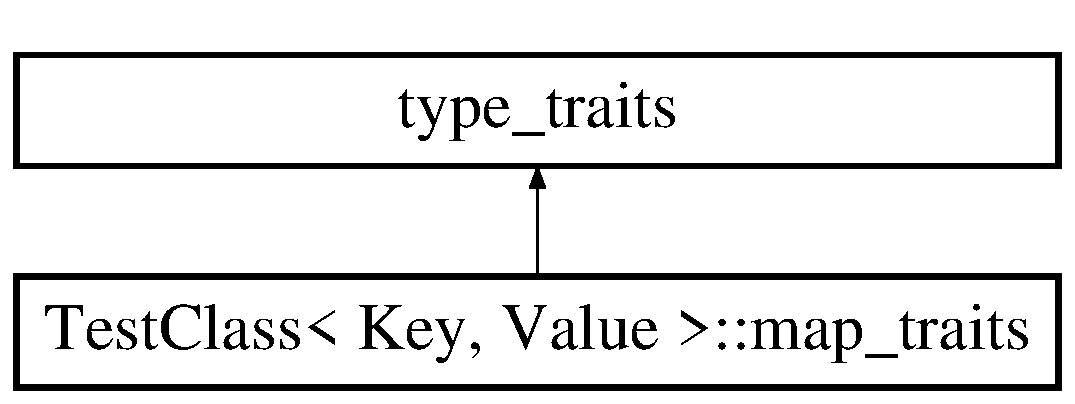
\includegraphics[height=2.000000cm]{struct_test_class_1_1map__traits}
\end{center}
\end{figure}
\subsection*{Classes}
\begin{DoxyCompactItemize}
\item 
struct \hyperlink{struct_test_class_1_1map__traits_1_1hash}{hash}
\end{DoxyCompactItemize}


The documentation for this struct was generated from the following file\+:\begin{DoxyCompactItemize}
\item 
tervel/tests/hash\+\_\+map/api/\hyperlink{cds__michael__map_8h}{cds\+\_\+michael\+\_\+map.\+h}\end{DoxyCompactItemize}

\hypertarget{classtervel_1_1algorithms_1_1wf_1_1mcas_1_1_m_c_a_s}{}\section{tervel\+:\+:algorithms\+:\+:wf\+:\+:mcas\+:\+:M\+C\+A\+S$<$ T $>$ Class Template Reference}
\label{classtervel_1_1algorithms_1_1wf_1_1mcas_1_1_m_c_a_s}\index{tervel\+::algorithms\+::wf\+::mcas\+::\+M\+C\+A\+S$<$ T $>$@{tervel\+::algorithms\+::wf\+::mcas\+::\+M\+C\+A\+S$<$ T $>$}}


{\ttfamily \#include $<$mcas\+\_\+helper.\+h$>$}



The documentation for this class was generated from the following file\+:\begin{DoxyCompactItemize}
\item 
tervel/algorithms/wf/mcas/\hyperlink{mcas__helper_8h}{mcas\+\_\+helper.\+h}\end{DoxyCompactItemize}

\hypertarget{classtervel_1_1algorithms_1_1wf_1_1mcas_1_1_multi_word_compare_and_swap}{}\section{tervel\+:\+:algorithms\+:\+:wf\+:\+:mcas\+:\+:Multi\+Word\+Compare\+And\+Swap$<$ T $>$ Class Template Reference}
\label{classtervel_1_1algorithms_1_1wf_1_1mcas_1_1_multi_word_compare_and_swap}\index{tervel\+::algorithms\+::wf\+::mcas\+::\+Multi\+Word\+Compare\+And\+Swap$<$ T $>$@{tervel\+::algorithms\+::wf\+::mcas\+::\+Multi\+Word\+Compare\+And\+Swap$<$ T $>$}}


\hyperlink{classtervel_1_1algorithms_1_1wf_1_1mcas_1_1_multi_word_compare_and_swap}{Multi\+Word\+Compare\+And\+Swap} class is used to perform a Multi-\/\+Word Compare-\/and-\/\+Swap (\hyperlink{classtervel_1_1algorithms_1_1wf_1_1mcas_1_1_m_c_a_s}{M\+C\+A\+S}) To execute an \hyperlink{classtervel_1_1algorithms_1_1wf_1_1mcas_1_1_m_c_a_s}{M\+C\+A\+S}, call add\+C\+A\+S\+Triple for each address you want to update, then call \hyperlink{classtervel_1_1algorithms_1_1wf_1_1mcas_1_1_multi_word_compare_and_swap_a3cf56f32c7579f734b1e0ecbd8d9c7f3}{execute()};.  




{\ttfamily \#include $<$mcas.\+h$>$}

Inheritance diagram for tervel\+:\+:algorithms\+:\+:wf\+:\+:mcas\+:\+:Multi\+Word\+Compare\+And\+Swap$<$ T $>$\+:\begin{figure}[H]
\begin{center}
\leavevmode
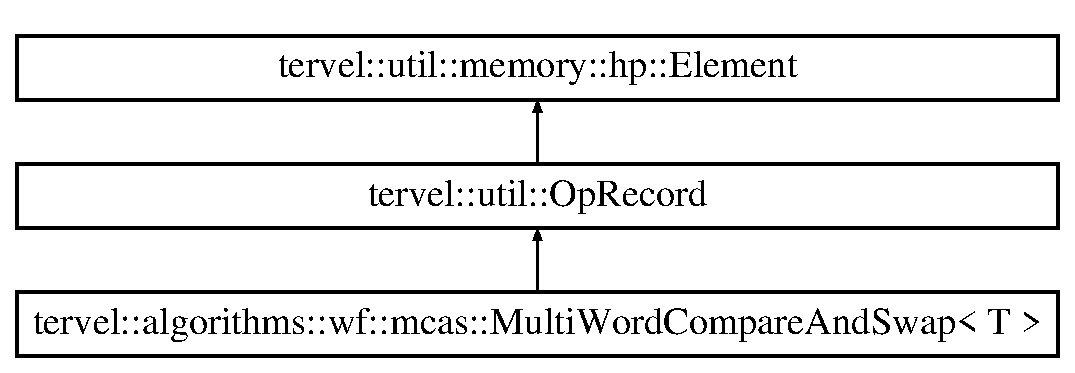
\includegraphics[height=3.000000cm]{classtervel_1_1algorithms_1_1wf_1_1mcas_1_1_multi_word_compare_and_swap}
\end{center}
\end{figure}
\subsection*{Public Member Functions}
\begin{DoxyCompactItemize}
\item 
\hyperlink{classtervel_1_1algorithms_1_1wf_1_1mcas_1_1_multi_word_compare_and_swap_ac31e0f21642273902a26d2858778c57c}{Multi\+Word\+Compare\+And\+Swap} (int max\+\_\+rows)
\item 
\hyperlink{classtervel_1_1algorithms_1_1wf_1_1mcas_1_1_multi_word_compare_and_swap_abb6ccc2c0fc9c52e741b4a7b544f4ec9}{$\sim$\+Multi\+Word\+Compare\+And\+Swap} ()
\item 
bool \hyperlink{classtervel_1_1algorithms_1_1wf_1_1mcas_1_1_multi_word_compare_and_swap_adb40351c3953d749ff9a57237730846a}{add\+\_\+cas\+\_\+triple} (std\+::atomic$<$ T $>$ $\ast$address, T expected\+\_\+value, T new\+\_\+value)
\begin{DoxyCompactList}\small\item\em This function is used to add a C\+A\+S triple to the \hyperlink{classtervel_1_1algorithms_1_1wf_1_1mcas_1_1_m_c_a_s}{M\+C\+A\+S} operation. \end{DoxyCompactList}\item 
bool \hyperlink{classtervel_1_1algorithms_1_1wf_1_1mcas_1_1_multi_word_compare_and_swap_a3cf56f32c7579f734b1e0ecbd8d9c7f3}{execute} ()
\begin{DoxyCompactList}\small\item\em This function is called after all the C\+A\+S triples have been added to the operation. \end{DoxyCompactList}\item 
void \hyperlink{classtervel_1_1algorithms_1_1wf_1_1mcas_1_1_multi_word_compare_and_swap_a2581e26f73e07c80473cf2999cf45652}{help\+\_\+complete} ()
\begin{DoxyCompactList}\small\item\em T\+His function overrides the virtual function in the Op\+Record class It is called by the progress assurance scheme. \end{DoxyCompactList}\item 
bool \hyperlink{classtervel_1_1algorithms_1_1wf_1_1mcas_1_1_multi_word_compare_and_swap_aa5ee7cf4770a925939b9e7497b34473a}{on\+\_\+is\+\_\+watched} ()
\begin{DoxyCompactList}\small\item\em This function overrides the virtual function in the H\+P\+::\+Element class It returns whether or not this mcas class is being referenced by another threaded. \end{DoxyCompactList}\end{DoxyCompactItemize}
\subsection*{Static Public Attributes}
\begin{DoxyCompactItemize}
\item 
static constexpr void $\ast$ \hyperlink{classtervel_1_1algorithms_1_1wf_1_1mcas_1_1_multi_word_compare_and_swap_a7f918a073a882ba1219855a9e03db2f6}{M\+C\+A\+S\+\_\+\+F\+A\+I\+L\+\_\+\+C\+O\+N\+S\+T} = reinterpret\+\_\+cast$<$void $\ast$$>$(0x1\+L)
\end{DoxyCompactItemize}
\subsection*{Private Types}
\begin{DoxyCompactItemize}
\item 
enum \hyperlink{classtervel_1_1algorithms_1_1wf_1_1mcas_1_1_multi_word_compare_and_swap_acc59b33256be2492c2d576bd1b770027}{M\+Cas\+State} \+: std\+::int8\+\_\+t \{ \hyperlink{classtervel_1_1algorithms_1_1wf_1_1mcas_1_1_multi_word_compare_and_swap_acc59b33256be2492c2d576bd1b770027aca69f96c768067fbff6c911ca87bccc9}{M\+Cas\+State\+::\+I\+N\+\_\+\+P\+R\+O\+G\+R\+E\+S\+S} = 0, 
\hyperlink{classtervel_1_1algorithms_1_1wf_1_1mcas_1_1_multi_word_compare_and_swap_acc59b33256be2492c2d576bd1b770027a7a95bf926a0333f57705aeac07a362a2}{M\+Cas\+State\+::\+P\+A\+S\+S} = 1, 
\hyperlink{classtervel_1_1algorithms_1_1wf_1_1mcas_1_1_multi_word_compare_and_swap_acc59b33256be2492c2d576bd1b770027ac2759effffc94bb9acc71d69fe3e8a1f}{M\+Cas\+State\+::\+F\+A\+I\+L} = 2, 
\hyperlink{classtervel_1_1algorithms_1_1wf_1_1mcas_1_1_multi_word_compare_and_swap_acc59b33256be2492c2d576bd1b770027a63c2867fdcae0e8e8413d7ac21b69b59}{M\+Cas\+State\+::\+D\+E\+L\+E\+T\+E\+D} = 3
 \}\begin{DoxyCompactList}\small\item\em This enum is used to indicate the state of an mcas operation D\+E\+L\+E\+T\+E\+D is used in debugging procedures. \end{DoxyCompactList}
\end{DoxyCompactItemize}
\subsection*{Private Member Functions}
\begin{DoxyCompactItemize}
\item 
bool \hyperlink{classtervel_1_1algorithms_1_1wf_1_1mcas_1_1_multi_word_compare_and_swap_a3336555d8271a621a8d616197719de94}{mcas\+\_\+complete} (int start\+\_\+pos, bool wfmode=false)
\begin{DoxyCompactList}\small\item\em This function is used to complete a currently executing \hyperlink{classtervel_1_1algorithms_1_1wf_1_1mcas_1_1_m_c_a_s}{M\+C\+A\+S} operation It is most likely that this operation is in conflict with some other operation and that it was discover by the dereferencing of an M\+C\+H The M\+C\+H contains a reference to the row in the \hyperlink{classtervel_1_1algorithms_1_1wf_1_1mcas_1_1_m_c_a_s}{M\+C\+A\+S} it is associated with and a reference to the final row in the mcas. \end{DoxyCompactList}\item 
bool \hyperlink{classtervel_1_1algorithms_1_1wf_1_1mcas_1_1_multi_word_compare_and_swap_a7cfccaf9f649f972039aaae8634989ec}{mcas\+\_\+complete} (\hyperlink{classtervel_1_1algorithms_1_1wf_1_1mcas_1_1_cas_row}{Cas\+Row}$<$ T $>$ $\ast$current\+\_\+row)
\begin{DoxyCompactList}\small\item\em Same as above, but it calculates the start\+\_\+pos based on the current row then calls the above mcas\+\_\+complete. \end{DoxyCompactList}\item 
void \hyperlink{classtervel_1_1algorithms_1_1wf_1_1mcas_1_1_multi_word_compare_and_swap_a66dbc5cd0e815dd1884ae39e432ad44d}{cleanup} (bool success)
\begin{DoxyCompactList}\small\item\em This function is used to cleanup a completed \hyperlink{classtervel_1_1algorithms_1_1wf_1_1mcas_1_1_m_c_a_s}{M\+C\+A\+S} operation It removes each M\+C\+H placed during this operation, replacing it with the logical value. \end{DoxyCompactList}\item 
T \hyperlink{classtervel_1_1algorithms_1_1wf_1_1mcas_1_1_multi_word_compare_and_swap_a2bd338dc83ac629d5c139f74eab2f5d7}{mcas\+\_\+remove} (const int pos, T value)
\begin{DoxyCompactList}\small\item\em This function insures that upon its return that $\ast$(cas\+\_\+rows\+\_\+\mbox{[}pos\mbox{]}.address) no longer equals value. \end{DoxyCompactList}\end{DoxyCompactItemize}
\subsection*{Private Attributes}
\begin{DoxyCompactItemize}
\item 
std\+::unique\+\_\+ptr$<$ \hyperlink{classtervel_1_1algorithms_1_1wf_1_1mcas_1_1_cas_row}{Cas\+Row}$<$ T $>$\mbox{[}$\,$\mbox{]}$>$ \hyperlink{classtervel_1_1algorithms_1_1wf_1_1mcas_1_1_multi_word_compare_and_swap_aa8be0b396445ce9d7e022aaab4acbaff}{cas\+\_\+rows\+\_\+}
\item 
std\+::atomic$<$ \hyperlink{classtervel_1_1algorithms_1_1wf_1_1mcas_1_1_multi_word_compare_and_swap_acc59b33256be2492c2d576bd1b770027}{M\+Cas\+State} $>$ \hyperlink{classtervel_1_1algorithms_1_1wf_1_1mcas_1_1_multi_word_compare_and_swap_a4d1104bb3f8bd1f0c2f4f93366c08224}{state\+\_\+} \{\hyperlink{classtervel_1_1algorithms_1_1wf_1_1mcas_1_1_multi_word_compare_and_swap_acc59b33256be2492c2d576bd1b770027aca69f96c768067fbff6c911ca87bccc9}{M\+Cas\+State\+::\+I\+N\+\_\+\+P\+R\+O\+G\+R\+E\+S\+S}\}
\item 
int \hyperlink{classtervel_1_1algorithms_1_1wf_1_1mcas_1_1_multi_word_compare_and_swap_a7e5a630e068ea866a43d4ad17fe71b98}{row\+\_\+count\+\_\+} \{0\}
\item 
int \hyperlink{classtervel_1_1algorithms_1_1wf_1_1mcas_1_1_multi_word_compare_and_swap_a9a61156a897ca69db4ef4b14a3949b5f}{max\+\_\+rows\+\_\+}
\item 
friend \hyperlink{classtervel_1_1algorithms_1_1wf_1_1mcas_1_1_multi_word_compare_and_swap_afdcffdc9d34879f8028a39d91def8fb7}{Helper$<$ T $>$}
\item 
friend \hyperlink{classtervel_1_1algorithms_1_1wf_1_1mcas_1_1_multi_word_compare_and_swap_a330cbacbf84e4c22631cc35b28b0bed4}{Cas\+Row$<$ T $>$}
\end{DoxyCompactItemize}


\subsection{Detailed Description}
\subsubsection*{template$<$class T$>$class tervel\+::algorithms\+::wf\+::mcas\+::\+Multi\+Word\+Compare\+And\+Swap$<$ T $>$}

\hyperlink{classtervel_1_1algorithms_1_1wf_1_1mcas_1_1_multi_word_compare_and_swap}{Multi\+Word\+Compare\+And\+Swap} class is used to perform a Multi-\/\+Word Compare-\/and-\/\+Swap (\hyperlink{classtervel_1_1algorithms_1_1wf_1_1mcas_1_1_m_c_a_s}{M\+C\+A\+S}) To execute an \hyperlink{classtervel_1_1algorithms_1_1wf_1_1mcas_1_1_m_c_a_s}{M\+C\+A\+S}, call add\+C\+A\+S\+Triple for each address you want to update, then call \hyperlink{classtervel_1_1algorithms_1_1wf_1_1mcas_1_1_multi_word_compare_and_swap_a3cf56f32c7579f734b1e0ecbd8d9c7f3}{execute()};. 

This function is wait-\/free. 

\subsection{Member Enumeration Documentation}
\hypertarget{classtervel_1_1algorithms_1_1wf_1_1mcas_1_1_multi_word_compare_and_swap_acc59b33256be2492c2d576bd1b770027}{}\index{tervel\+::algorithms\+::wf\+::mcas\+::\+Multi\+Word\+Compare\+And\+Swap@{tervel\+::algorithms\+::wf\+::mcas\+::\+Multi\+Word\+Compare\+And\+Swap}!M\+Cas\+State@{M\+Cas\+State}}
\index{M\+Cas\+State@{M\+Cas\+State}!tervel\+::algorithms\+::wf\+::mcas\+::\+Multi\+Word\+Compare\+And\+Swap@{tervel\+::algorithms\+::wf\+::mcas\+::\+Multi\+Word\+Compare\+And\+Swap}}
\subsubsection[{M\+Cas\+State}]{\setlength{\rightskip}{0pt plus 5cm}template$<$class T $>$ enum {\bf tervel\+::algorithms\+::wf\+::mcas\+::\+Multi\+Word\+Compare\+And\+Swap\+::\+M\+Cas\+State} \+: std\+::int8\+\_\+t\hspace{0.3cm}{\ttfamily [strong]}, {\ttfamily [private]}}\label{classtervel_1_1algorithms_1_1wf_1_1mcas_1_1_multi_word_compare_and_swap_acc59b33256be2492c2d576bd1b770027}


This enum is used to indicate the state of an mcas operation D\+E\+L\+E\+T\+E\+D is used in debugging procedures. 

\begin{Desc}
\item[Enumerator]\par
\begin{description}
\index{I\+N\+\_\+\+P\+R\+O\+G\+R\+E\+S\+S@{I\+N\+\_\+\+P\+R\+O\+G\+R\+E\+S\+S}!tervel\+::algorithms\+::wf\+::mcas\+::\+Multi\+Word\+Compare\+And\+Swap@{tervel\+::algorithms\+::wf\+::mcas\+::\+Multi\+Word\+Compare\+And\+Swap}}\index{tervel\+::algorithms\+::wf\+::mcas\+::\+Multi\+Word\+Compare\+And\+Swap@{tervel\+::algorithms\+::wf\+::mcas\+::\+Multi\+Word\+Compare\+And\+Swap}!I\+N\+\_\+\+P\+R\+O\+G\+R\+E\+S\+S@{I\+N\+\_\+\+P\+R\+O\+G\+R\+E\+S\+S}}\item[{\em 
\hypertarget{classtervel_1_1algorithms_1_1wf_1_1mcas_1_1_multi_word_compare_and_swap_acc59b33256be2492c2d576bd1b770027aca69f96c768067fbff6c911ca87bccc9}{}I\+N\+\_\+\+P\+R\+O\+G\+R\+E\+S\+S\label{classtervel_1_1algorithms_1_1wf_1_1mcas_1_1_multi_word_compare_and_swap_acc59b33256be2492c2d576bd1b770027aca69f96c768067fbff6c911ca87bccc9}
}]\index{P\+A\+S\+S@{P\+A\+S\+S}!tervel\+::algorithms\+::wf\+::mcas\+::\+Multi\+Word\+Compare\+And\+Swap@{tervel\+::algorithms\+::wf\+::mcas\+::\+Multi\+Word\+Compare\+And\+Swap}}\index{tervel\+::algorithms\+::wf\+::mcas\+::\+Multi\+Word\+Compare\+And\+Swap@{tervel\+::algorithms\+::wf\+::mcas\+::\+Multi\+Word\+Compare\+And\+Swap}!P\+A\+S\+S@{P\+A\+S\+S}}\item[{\em 
\hypertarget{classtervel_1_1algorithms_1_1wf_1_1mcas_1_1_multi_word_compare_and_swap_acc59b33256be2492c2d576bd1b770027a7a95bf926a0333f57705aeac07a362a2}{}P\+A\+S\+S\label{classtervel_1_1algorithms_1_1wf_1_1mcas_1_1_multi_word_compare_and_swap_acc59b33256be2492c2d576bd1b770027a7a95bf926a0333f57705aeac07a362a2}
}]\index{F\+A\+I\+L@{F\+A\+I\+L}!tervel\+::algorithms\+::wf\+::mcas\+::\+Multi\+Word\+Compare\+And\+Swap@{tervel\+::algorithms\+::wf\+::mcas\+::\+Multi\+Word\+Compare\+And\+Swap}}\index{tervel\+::algorithms\+::wf\+::mcas\+::\+Multi\+Word\+Compare\+And\+Swap@{tervel\+::algorithms\+::wf\+::mcas\+::\+Multi\+Word\+Compare\+And\+Swap}!F\+A\+I\+L@{F\+A\+I\+L}}\item[{\em 
\hypertarget{classtervel_1_1algorithms_1_1wf_1_1mcas_1_1_multi_word_compare_and_swap_acc59b33256be2492c2d576bd1b770027ac2759effffc94bb9acc71d69fe3e8a1f}{}F\+A\+I\+L\label{classtervel_1_1algorithms_1_1wf_1_1mcas_1_1_multi_word_compare_and_swap_acc59b33256be2492c2d576bd1b770027ac2759effffc94bb9acc71d69fe3e8a1f}
}]\index{D\+E\+L\+E\+T\+E\+D@{D\+E\+L\+E\+T\+E\+D}!tervel\+::algorithms\+::wf\+::mcas\+::\+Multi\+Word\+Compare\+And\+Swap@{tervel\+::algorithms\+::wf\+::mcas\+::\+Multi\+Word\+Compare\+And\+Swap}}\index{tervel\+::algorithms\+::wf\+::mcas\+::\+Multi\+Word\+Compare\+And\+Swap@{tervel\+::algorithms\+::wf\+::mcas\+::\+Multi\+Word\+Compare\+And\+Swap}!D\+E\+L\+E\+T\+E\+D@{D\+E\+L\+E\+T\+E\+D}}\item[{\em 
\hypertarget{classtervel_1_1algorithms_1_1wf_1_1mcas_1_1_multi_word_compare_and_swap_acc59b33256be2492c2d576bd1b770027a63c2867fdcae0e8e8413d7ac21b69b59}{}D\+E\+L\+E\+T\+E\+D\label{classtervel_1_1algorithms_1_1wf_1_1mcas_1_1_multi_word_compare_and_swap_acc59b33256be2492c2d576bd1b770027a63c2867fdcae0e8e8413d7ac21b69b59}
}]\end{description}
\end{Desc}


\subsection{Constructor \& Destructor Documentation}
\hypertarget{classtervel_1_1algorithms_1_1wf_1_1mcas_1_1_multi_word_compare_and_swap_ac31e0f21642273902a26d2858778c57c}{}\index{tervel\+::algorithms\+::wf\+::mcas\+::\+Multi\+Word\+Compare\+And\+Swap@{tervel\+::algorithms\+::wf\+::mcas\+::\+Multi\+Word\+Compare\+And\+Swap}!Multi\+Word\+Compare\+And\+Swap@{Multi\+Word\+Compare\+And\+Swap}}
\index{Multi\+Word\+Compare\+And\+Swap@{Multi\+Word\+Compare\+And\+Swap}!tervel\+::algorithms\+::wf\+::mcas\+::\+Multi\+Word\+Compare\+And\+Swap@{tervel\+::algorithms\+::wf\+::mcas\+::\+Multi\+Word\+Compare\+And\+Swap}}
\subsubsection[{Multi\+Word\+Compare\+And\+Swap(int max\+\_\+rows)}]{\setlength{\rightskip}{0pt plus 5cm}template$<$class T $>$ {\bf tervel\+::algorithms\+::wf\+::mcas\+::\+Multi\+Word\+Compare\+And\+Swap}$<$ T $>$\+::{\bf Multi\+Word\+Compare\+And\+Swap} (
\begin{DoxyParamCaption}
\item[{int}]{max\+\_\+rows}
\end{DoxyParamCaption}
)\hspace{0.3cm}{\ttfamily [inline]}, {\ttfamily [explicit]}}\label{classtervel_1_1algorithms_1_1wf_1_1mcas_1_1_multi_word_compare_and_swap_ac31e0f21642273902a26d2858778c57c}
\hypertarget{classtervel_1_1algorithms_1_1wf_1_1mcas_1_1_multi_word_compare_and_swap_abb6ccc2c0fc9c52e741b4a7b544f4ec9}{}\index{tervel\+::algorithms\+::wf\+::mcas\+::\+Multi\+Word\+Compare\+And\+Swap@{tervel\+::algorithms\+::wf\+::mcas\+::\+Multi\+Word\+Compare\+And\+Swap}!````~Multi\+Word\+Compare\+And\+Swap@{$\sim$\+Multi\+Word\+Compare\+And\+Swap}}
\index{````~Multi\+Word\+Compare\+And\+Swap@{$\sim$\+Multi\+Word\+Compare\+And\+Swap}!tervel\+::algorithms\+::wf\+::mcas\+::\+Multi\+Word\+Compare\+And\+Swap@{tervel\+::algorithms\+::wf\+::mcas\+::\+Multi\+Word\+Compare\+And\+Swap}}
\subsubsection[{$\sim$\+Multi\+Word\+Compare\+And\+Swap()}]{\setlength{\rightskip}{0pt plus 5cm}template$<$class T $>$ {\bf tervel\+::algorithms\+::wf\+::mcas\+::\+Multi\+Word\+Compare\+And\+Swap}$<$ T $>$\+::$\sim${\bf Multi\+Word\+Compare\+And\+Swap} (
\begin{DoxyParamCaption}
{}
\end{DoxyParamCaption}
)\hspace{0.3cm}{\ttfamily [inline]}}\label{classtervel_1_1algorithms_1_1wf_1_1mcas_1_1_multi_word_compare_and_swap_abb6ccc2c0fc9c52e741b4a7b544f4ec9}


\subsection{Member Function Documentation}
\hypertarget{classtervel_1_1algorithms_1_1wf_1_1mcas_1_1_multi_word_compare_and_swap_adb40351c3953d749ff9a57237730846a}{}\index{tervel\+::algorithms\+::wf\+::mcas\+::\+Multi\+Word\+Compare\+And\+Swap@{tervel\+::algorithms\+::wf\+::mcas\+::\+Multi\+Word\+Compare\+And\+Swap}!add\+\_\+cas\+\_\+triple@{add\+\_\+cas\+\_\+triple}}
\index{add\+\_\+cas\+\_\+triple@{add\+\_\+cas\+\_\+triple}!tervel\+::algorithms\+::wf\+::mcas\+::\+Multi\+Word\+Compare\+And\+Swap@{tervel\+::algorithms\+::wf\+::mcas\+::\+Multi\+Word\+Compare\+And\+Swap}}
\subsubsection[{add\+\_\+cas\+\_\+triple(std\+::atomic$<$ T $>$ $\ast$address, T expected\+\_\+value, T new\+\_\+value)}]{\setlength{\rightskip}{0pt plus 5cm}template$<$class T $>$ bool {\bf tervel\+::algorithms\+::wf\+::mcas\+::\+Multi\+Word\+Compare\+And\+Swap}$<$ T $>$\+::add\+\_\+cas\+\_\+triple (
\begin{DoxyParamCaption}
\item[{std\+::atomic$<$ T $>$ $\ast$}]{address, }
\item[{T}]{expected\+\_\+value, }
\item[{T}]{new\+\_\+value}
\end{DoxyParamCaption}
)}\label{classtervel_1_1algorithms_1_1wf_1_1mcas_1_1_multi_word_compare_and_swap_adb40351c3953d749ff9a57237730846a}


This function is used to add a C\+A\+S triple to the \hyperlink{classtervel_1_1algorithms_1_1wf_1_1mcas_1_1_m_c_a_s}{M\+C\+A\+S} operation. 

Each Triple consistent of an address to replace the expected value with a new value iff each other address holds its expected value.

This function returns false in the event the address already exists in the \hyperlink{classtervel_1_1algorithms_1_1wf_1_1mcas_1_1_m_c_a_s}{M\+C\+A\+S} operation or the passed values are not valid. A Valid value is a value which does not use one of the reserved bits or constants. See related documentation for more details


\begin{DoxyParams}{Parameters}
{\em address} & \\
\hline
{\em expected\+\_\+value} & \\
\hline
{\em new\+\_\+value} & \\
\hline
\end{DoxyParams}
\begin{DoxyReturn}{Returns}
true if successfully added. 
\end{DoxyReturn}
\hypertarget{classtervel_1_1algorithms_1_1wf_1_1mcas_1_1_multi_word_compare_and_swap_a66dbc5cd0e815dd1884ae39e432ad44d}{}\index{tervel\+::algorithms\+::wf\+::mcas\+::\+Multi\+Word\+Compare\+And\+Swap@{tervel\+::algorithms\+::wf\+::mcas\+::\+Multi\+Word\+Compare\+And\+Swap}!cleanup@{cleanup}}
\index{cleanup@{cleanup}!tervel\+::algorithms\+::wf\+::mcas\+::\+Multi\+Word\+Compare\+And\+Swap@{tervel\+::algorithms\+::wf\+::mcas\+::\+Multi\+Word\+Compare\+And\+Swap}}
\subsubsection[{cleanup(bool success)}]{\setlength{\rightskip}{0pt plus 5cm}template$<$class T $>$ void {\bf tervel\+::algorithms\+::wf\+::mcas\+::\+Multi\+Word\+Compare\+And\+Swap}$<$ T $>$\+::cleanup (
\begin{DoxyParamCaption}
\item[{bool}]{success}
\end{DoxyParamCaption}
)\hspace{0.3cm}{\ttfamily [private]}}\label{classtervel_1_1algorithms_1_1wf_1_1mcas_1_1_multi_word_compare_and_swap_a66dbc5cd0e815dd1884ae39e432ad44d}


This function is used to cleanup a completed \hyperlink{classtervel_1_1algorithms_1_1wf_1_1mcas_1_1_m_c_a_s}{M\+C\+A\+S} operation It removes each M\+C\+H placed during this operation, replacing it with the logical value. 

\hypertarget{classtervel_1_1algorithms_1_1wf_1_1mcas_1_1_multi_word_compare_and_swap_a3cf56f32c7579f734b1e0ecbd8d9c7f3}{}\index{tervel\+::algorithms\+::wf\+::mcas\+::\+Multi\+Word\+Compare\+And\+Swap@{tervel\+::algorithms\+::wf\+::mcas\+::\+Multi\+Word\+Compare\+And\+Swap}!execute@{execute}}
\index{execute@{execute}!tervel\+::algorithms\+::wf\+::mcas\+::\+Multi\+Word\+Compare\+And\+Swap@{tervel\+::algorithms\+::wf\+::mcas\+::\+Multi\+Word\+Compare\+And\+Swap}}
\subsubsection[{execute()}]{\setlength{\rightskip}{0pt plus 5cm}template$<$class T $>$ bool {\bf tervel\+::algorithms\+::wf\+::mcas\+::\+Multi\+Word\+Compare\+And\+Swap}$<$ T $>$\+::execute (
\begin{DoxyParamCaption}
{}
\end{DoxyParamCaption}
)}\label{classtervel_1_1algorithms_1_1wf_1_1mcas_1_1_multi_word_compare_and_swap_a3cf56f32c7579f734b1e0ecbd8d9c7f3}


This function is called after all the C\+A\+S triples have been added to the operation. 

It will attempt to apply the operation.

\begin{DoxyReturn}{Returns}
true if it replaced the values at each address with a new value 
\end{DoxyReturn}
\hypertarget{classtervel_1_1algorithms_1_1wf_1_1mcas_1_1_multi_word_compare_and_swap_a2581e26f73e07c80473cf2999cf45652}{}\index{tervel\+::algorithms\+::wf\+::mcas\+::\+Multi\+Word\+Compare\+And\+Swap@{tervel\+::algorithms\+::wf\+::mcas\+::\+Multi\+Word\+Compare\+And\+Swap}!help\+\_\+complete@{help\+\_\+complete}}
\index{help\+\_\+complete@{help\+\_\+complete}!tervel\+::algorithms\+::wf\+::mcas\+::\+Multi\+Word\+Compare\+And\+Swap@{tervel\+::algorithms\+::wf\+::mcas\+::\+Multi\+Word\+Compare\+And\+Swap}}
\subsubsection[{help\+\_\+complete()}]{\setlength{\rightskip}{0pt plus 5cm}template$<$class T $>$ void {\bf tervel\+::algorithms\+::wf\+::mcas\+::\+Multi\+Word\+Compare\+And\+Swap}$<$ T $>$\+::help\+\_\+complete (
\begin{DoxyParamCaption}
{}
\end{DoxyParamCaption}
)\hspace{0.3cm}{\ttfamily [inline]}, {\ttfamily [virtual]}}\label{classtervel_1_1algorithms_1_1wf_1_1mcas_1_1_multi_word_compare_and_swap_a2581e26f73e07c80473cf2999cf45652}


T\+His function overrides the virtual function in the Op\+Record class It is called by the progress assurance scheme. 

Upon its return the \hyperlink{classtervel_1_1algorithms_1_1wf_1_1mcas_1_1_m_c_a_s}{M\+C\+A\+S} operation must be completed 

Implements \hyperlink{classtervel_1_1util_1_1_op_record_aa75ab39688a8d4cceb6a1ef0409537c0}{tervel\+::util\+::\+Op\+Record}.

\hypertarget{classtervel_1_1algorithms_1_1wf_1_1mcas_1_1_multi_word_compare_and_swap_a3336555d8271a621a8d616197719de94}{}\index{tervel\+::algorithms\+::wf\+::mcas\+::\+Multi\+Word\+Compare\+And\+Swap@{tervel\+::algorithms\+::wf\+::mcas\+::\+Multi\+Word\+Compare\+And\+Swap}!mcas\+\_\+complete@{mcas\+\_\+complete}}
\index{mcas\+\_\+complete@{mcas\+\_\+complete}!tervel\+::algorithms\+::wf\+::mcas\+::\+Multi\+Word\+Compare\+And\+Swap@{tervel\+::algorithms\+::wf\+::mcas\+::\+Multi\+Word\+Compare\+And\+Swap}}
\subsubsection[{mcas\+\_\+complete(int start\+\_\+pos, bool wfmode=false)}]{\setlength{\rightskip}{0pt plus 5cm}template$<$class T $>$ bool {\bf tervel\+::algorithms\+::wf\+::mcas\+::\+Multi\+Word\+Compare\+And\+Swap}$<$ T $>$\+::mcas\+\_\+complete (
\begin{DoxyParamCaption}
\item[{int}]{start\+\_\+pos, }
\item[{bool}]{wfmode = {\ttfamily false}}
\end{DoxyParamCaption}
)\hspace{0.3cm}{\ttfamily [private]}}\label{classtervel_1_1algorithms_1_1wf_1_1mcas_1_1_multi_word_compare_and_swap_a3336555d8271a621a8d616197719de94}


This function is used to complete a currently executing \hyperlink{classtervel_1_1algorithms_1_1wf_1_1mcas_1_1_m_c_a_s}{M\+C\+A\+S} operation It is most likely that this operation is in conflict with some other operation and that it was discover by the dereferencing of an M\+C\+H The M\+C\+H contains a reference to the row in the \hyperlink{classtervel_1_1algorithms_1_1wf_1_1mcas_1_1_m_c_a_s}{M\+C\+A\+S} it is associated with and a reference to the final row in the mcas. 

Using these two, we can complete the remaining rows.


\begin{DoxyParams}{Parameters}
{\em start\+\_\+pos} & the row to begin at \\
\hline
{\em wfmode} & if true it ignores the fail count because the operation is in the op\+\_\+table \\
\hline
\end{DoxyParams}
\begin{DoxyReturn}{Returns}
whether or not the mcas succeeded. 
\end{DoxyReturn}
Loop for each row in the op, if helping complete another thread\textquotesingle{}s \hyperlink{classtervel_1_1algorithms_1_1wf_1_1mcas_1_1_m_c_a_s}{M\+C\+A\+S} Start at last known completed row.\hypertarget{classtervel_1_1algorithms_1_1wf_1_1mcas_1_1_multi_word_compare_and_swap_a7cfccaf9f649f972039aaae8634989ec}{}\index{tervel\+::algorithms\+::wf\+::mcas\+::\+Multi\+Word\+Compare\+And\+Swap@{tervel\+::algorithms\+::wf\+::mcas\+::\+Multi\+Word\+Compare\+And\+Swap}!mcas\+\_\+complete@{mcas\+\_\+complete}}
\index{mcas\+\_\+complete@{mcas\+\_\+complete}!tervel\+::algorithms\+::wf\+::mcas\+::\+Multi\+Word\+Compare\+And\+Swap@{tervel\+::algorithms\+::wf\+::mcas\+::\+Multi\+Word\+Compare\+And\+Swap}}
\subsubsection[{mcas\+\_\+complete(\+Cas\+Row$<$ T $>$ $\ast$current\+\_\+row)}]{\setlength{\rightskip}{0pt plus 5cm}template$<$class T $>$ bool {\bf tervel\+::algorithms\+::wf\+::mcas\+::\+Multi\+Word\+Compare\+And\+Swap}$<$ T $>$\+::mcas\+\_\+complete (
\begin{DoxyParamCaption}
\item[{{\bf Cas\+Row}$<$ T $>$ $\ast$}]{current\+\_\+row}
\end{DoxyParamCaption}
)\hspace{0.3cm}{\ttfamily [private]}}\label{classtervel_1_1algorithms_1_1wf_1_1mcas_1_1_multi_word_compare_and_swap_a7cfccaf9f649f972039aaae8634989ec}


Same as above, but it calculates the start\+\_\+pos based on the current row then calls the above mcas\+\_\+complete. 


\begin{DoxyParams}{Parameters}
{\em current\+\_\+row} & the last known completed row \\
\hline
\end{DoxyParams}
\begin{DoxyReturn}{Returns}
where or not the mcas succeeded 
\end{DoxyReturn}
\hypertarget{classtervel_1_1algorithms_1_1wf_1_1mcas_1_1_multi_word_compare_and_swap_a2bd338dc83ac629d5c139f74eab2f5d7}{}\index{tervel\+::algorithms\+::wf\+::mcas\+::\+Multi\+Word\+Compare\+And\+Swap@{tervel\+::algorithms\+::wf\+::mcas\+::\+Multi\+Word\+Compare\+And\+Swap}!mcas\+\_\+remove@{mcas\+\_\+remove}}
\index{mcas\+\_\+remove@{mcas\+\_\+remove}!tervel\+::algorithms\+::wf\+::mcas\+::\+Multi\+Word\+Compare\+And\+Swap@{tervel\+::algorithms\+::wf\+::mcas\+::\+Multi\+Word\+Compare\+And\+Swap}}
\subsubsection[{mcas\+\_\+remove(const int pos, T value)}]{\setlength{\rightskip}{0pt plus 5cm}template$<$class T $>$ T {\bf tervel\+::algorithms\+::wf\+::mcas\+::\+Multi\+Word\+Compare\+And\+Swap}$<$ T $>$\+::mcas\+\_\+remove (
\begin{DoxyParamCaption}
\item[{const int}]{pos, }
\item[{T}]{value}
\end{DoxyParamCaption}
)\hspace{0.3cm}{\ttfamily [private]}}\label{classtervel_1_1algorithms_1_1wf_1_1mcas_1_1_multi_word_compare_and_swap_a2bd338dc83ac629d5c139f74eab2f5d7}


This function insures that upon its return that $\ast$(cas\+\_\+rows\+\_\+\mbox{[}pos\mbox{]}.address) no longer equals value. 

Where value is an object that holds an R\+C bit mark. If the object is not a \hyperlink{classtervel_1_1algorithms_1_1wf_1_1mcas_1_1_helper}{Helper} for this operation, then the standard descriptor remove function is called. This is important to prevent the case where the stack increases beyond reasonable levels when multiple threads are helping to complete the same operation.


\begin{DoxyParams}{Parameters}
{\em pos} & the cas\+\_\+row which is blocked from completing its operation \\
\hline
{\em value} & the value read at the position \\
\hline
\end{DoxyParams}
\begin{DoxyReturn}{Returns}
the new current value 
\end{DoxyReturn}
\hypertarget{classtervel_1_1algorithms_1_1wf_1_1mcas_1_1_multi_word_compare_and_swap_aa5ee7cf4770a925939b9e7497b34473a}{}\index{tervel\+::algorithms\+::wf\+::mcas\+::\+Multi\+Word\+Compare\+And\+Swap@{tervel\+::algorithms\+::wf\+::mcas\+::\+Multi\+Word\+Compare\+And\+Swap}!on\+\_\+is\+\_\+watched@{on\+\_\+is\+\_\+watched}}
\index{on\+\_\+is\+\_\+watched@{on\+\_\+is\+\_\+watched}!tervel\+::algorithms\+::wf\+::mcas\+::\+Multi\+Word\+Compare\+And\+Swap@{tervel\+::algorithms\+::wf\+::mcas\+::\+Multi\+Word\+Compare\+And\+Swap}}
\subsubsection[{on\+\_\+is\+\_\+watched()}]{\setlength{\rightskip}{0pt plus 5cm}template$<$class T $>$ bool {\bf tervel\+::algorithms\+::wf\+::mcas\+::\+Multi\+Word\+Compare\+And\+Swap}$<$ T $>$\+::on\+\_\+is\+\_\+watched (
\begin{DoxyParamCaption}
{}
\end{DoxyParamCaption}
)\hspace{0.3cm}{\ttfamily [inline]}, {\ttfamily [virtual]}}\label{classtervel_1_1algorithms_1_1wf_1_1mcas_1_1_multi_word_compare_and_swap_aa5ee7cf4770a925939b9e7497b34473a}


This function overrides the virtual function in the H\+P\+::\+Element class It returns whether or not this mcas class is being referenced by another threaded. 

It is being referenced if any associated descriptor has a positive reference count or if there is a hazard point watch on it.

\begin{DoxyReturn}{Returns}
True if watched 
\end{DoxyReturn}


Reimplemented from \hyperlink{classtervel_1_1util_1_1memory_1_1hp_1_1_element_a88306bc6b64d0110e3ee568514dbcc04}{tervel\+::util\+::memory\+::hp\+::\+Element}.



\subsection{Member Data Documentation}
\hypertarget{classtervel_1_1algorithms_1_1wf_1_1mcas_1_1_multi_word_compare_and_swap_aa8be0b396445ce9d7e022aaab4acbaff}{}\index{tervel\+::algorithms\+::wf\+::mcas\+::\+Multi\+Word\+Compare\+And\+Swap@{tervel\+::algorithms\+::wf\+::mcas\+::\+Multi\+Word\+Compare\+And\+Swap}!cas\+\_\+rows\+\_\+@{cas\+\_\+rows\+\_\+}}
\index{cas\+\_\+rows\+\_\+@{cas\+\_\+rows\+\_\+}!tervel\+::algorithms\+::wf\+::mcas\+::\+Multi\+Word\+Compare\+And\+Swap@{tervel\+::algorithms\+::wf\+::mcas\+::\+Multi\+Word\+Compare\+And\+Swap}}
\subsubsection[{cas\+\_\+rows\+\_\+}]{\setlength{\rightskip}{0pt plus 5cm}template$<$class T $>$ std\+::unique\+\_\+ptr$<${\bf Cas\+Row}$<$T$>$\mbox{[}$\,$\mbox{]}$>$ {\bf tervel\+::algorithms\+::wf\+::mcas\+::\+Multi\+Word\+Compare\+And\+Swap}$<$ T $>$\+::cas\+\_\+rows\+\_\+\hspace{0.3cm}{\ttfamily [private]}}\label{classtervel_1_1algorithms_1_1wf_1_1mcas_1_1_multi_word_compare_and_swap_aa8be0b396445ce9d7e022aaab4acbaff}
\hypertarget{classtervel_1_1algorithms_1_1wf_1_1mcas_1_1_multi_word_compare_and_swap_a330cbacbf84e4c22631cc35b28b0bed4}{}\index{tervel\+::algorithms\+::wf\+::mcas\+::\+Multi\+Word\+Compare\+And\+Swap@{tervel\+::algorithms\+::wf\+::mcas\+::\+Multi\+Word\+Compare\+And\+Swap}!Cas\+Row$<$ T $>$@{Cas\+Row$<$ T $>$}}
\index{Cas\+Row$<$ T $>$@{Cas\+Row$<$ T $>$}!tervel\+::algorithms\+::wf\+::mcas\+::\+Multi\+Word\+Compare\+And\+Swap@{tervel\+::algorithms\+::wf\+::mcas\+::\+Multi\+Word\+Compare\+And\+Swap}}
\subsubsection[{Cas\+Row$<$ T $>$}]{\setlength{\rightskip}{0pt plus 5cm}template$<$class T $>$ friend {\bf tervel\+::algorithms\+::wf\+::mcas\+::\+Multi\+Word\+Compare\+And\+Swap}$<$ T $>$\+::{\bf Cas\+Row}$<$ T $>$\hspace{0.3cm}{\ttfamily [private]}}\label{classtervel_1_1algorithms_1_1wf_1_1mcas_1_1_multi_word_compare_and_swap_a330cbacbf84e4c22631cc35b28b0bed4}
\hypertarget{classtervel_1_1algorithms_1_1wf_1_1mcas_1_1_multi_word_compare_and_swap_afdcffdc9d34879f8028a39d91def8fb7}{}\index{tervel\+::algorithms\+::wf\+::mcas\+::\+Multi\+Word\+Compare\+And\+Swap@{tervel\+::algorithms\+::wf\+::mcas\+::\+Multi\+Word\+Compare\+And\+Swap}!Helper$<$ T $>$@{Helper$<$ T $>$}}
\index{Helper$<$ T $>$@{Helper$<$ T $>$}!tervel\+::algorithms\+::wf\+::mcas\+::\+Multi\+Word\+Compare\+And\+Swap@{tervel\+::algorithms\+::wf\+::mcas\+::\+Multi\+Word\+Compare\+And\+Swap}}
\subsubsection[{Helper$<$ T $>$}]{\setlength{\rightskip}{0pt plus 5cm}template$<$class T $>$ friend {\bf tervel\+::algorithms\+::wf\+::mcas\+::\+Multi\+Word\+Compare\+And\+Swap}$<$ T $>$\+::{\bf Helper}$<$ T $>$\hspace{0.3cm}{\ttfamily [private]}}\label{classtervel_1_1algorithms_1_1wf_1_1mcas_1_1_multi_word_compare_and_swap_afdcffdc9d34879f8028a39d91def8fb7}
\hypertarget{classtervel_1_1algorithms_1_1wf_1_1mcas_1_1_multi_word_compare_and_swap_a9a61156a897ca69db4ef4b14a3949b5f}{}\index{tervel\+::algorithms\+::wf\+::mcas\+::\+Multi\+Word\+Compare\+And\+Swap@{tervel\+::algorithms\+::wf\+::mcas\+::\+Multi\+Word\+Compare\+And\+Swap}!max\+\_\+rows\+\_\+@{max\+\_\+rows\+\_\+}}
\index{max\+\_\+rows\+\_\+@{max\+\_\+rows\+\_\+}!tervel\+::algorithms\+::wf\+::mcas\+::\+Multi\+Word\+Compare\+And\+Swap@{tervel\+::algorithms\+::wf\+::mcas\+::\+Multi\+Word\+Compare\+And\+Swap}}
\subsubsection[{max\+\_\+rows\+\_\+}]{\setlength{\rightskip}{0pt plus 5cm}template$<$class T $>$ int {\bf tervel\+::algorithms\+::wf\+::mcas\+::\+Multi\+Word\+Compare\+And\+Swap}$<$ T $>$\+::max\+\_\+rows\+\_\+\hspace{0.3cm}{\ttfamily [private]}}\label{classtervel_1_1algorithms_1_1wf_1_1mcas_1_1_multi_word_compare_and_swap_a9a61156a897ca69db4ef4b14a3949b5f}
\hypertarget{classtervel_1_1algorithms_1_1wf_1_1mcas_1_1_multi_word_compare_and_swap_a7f918a073a882ba1219855a9e03db2f6}{}\index{tervel\+::algorithms\+::wf\+::mcas\+::\+Multi\+Word\+Compare\+And\+Swap@{tervel\+::algorithms\+::wf\+::mcas\+::\+Multi\+Word\+Compare\+And\+Swap}!M\+C\+A\+S\+\_\+\+F\+A\+I\+L\+\_\+\+C\+O\+N\+S\+T@{M\+C\+A\+S\+\_\+\+F\+A\+I\+L\+\_\+\+C\+O\+N\+S\+T}}
\index{M\+C\+A\+S\+\_\+\+F\+A\+I\+L\+\_\+\+C\+O\+N\+S\+T@{M\+C\+A\+S\+\_\+\+F\+A\+I\+L\+\_\+\+C\+O\+N\+S\+T}!tervel\+::algorithms\+::wf\+::mcas\+::\+Multi\+Word\+Compare\+And\+Swap@{tervel\+::algorithms\+::wf\+::mcas\+::\+Multi\+Word\+Compare\+And\+Swap}}
\subsubsection[{M\+C\+A\+S\+\_\+\+F\+A\+I\+L\+\_\+\+C\+O\+N\+S\+T}]{\setlength{\rightskip}{0pt plus 5cm}template$<$class T $>$ constexpr void$\ast$ {\bf tervel\+::algorithms\+::wf\+::mcas\+::\+Multi\+Word\+Compare\+And\+Swap}$<$ T $>$\+::M\+C\+A\+S\+\_\+\+F\+A\+I\+L\+\_\+\+C\+O\+N\+S\+T = reinterpret\+\_\+cast$<$void $\ast$$>$(0x1\+L)\hspace{0.3cm}{\ttfamily [static]}}\label{classtervel_1_1algorithms_1_1wf_1_1mcas_1_1_multi_word_compare_and_swap_a7f918a073a882ba1219855a9e03db2f6}
\hypertarget{classtervel_1_1algorithms_1_1wf_1_1mcas_1_1_multi_word_compare_and_swap_a7e5a630e068ea866a43d4ad17fe71b98}{}\index{tervel\+::algorithms\+::wf\+::mcas\+::\+Multi\+Word\+Compare\+And\+Swap@{tervel\+::algorithms\+::wf\+::mcas\+::\+Multi\+Word\+Compare\+And\+Swap}!row\+\_\+count\+\_\+@{row\+\_\+count\+\_\+}}
\index{row\+\_\+count\+\_\+@{row\+\_\+count\+\_\+}!tervel\+::algorithms\+::wf\+::mcas\+::\+Multi\+Word\+Compare\+And\+Swap@{tervel\+::algorithms\+::wf\+::mcas\+::\+Multi\+Word\+Compare\+And\+Swap}}
\subsubsection[{row\+\_\+count\+\_\+}]{\setlength{\rightskip}{0pt plus 5cm}template$<$class T $>$ int {\bf tervel\+::algorithms\+::wf\+::mcas\+::\+Multi\+Word\+Compare\+And\+Swap}$<$ T $>$\+::row\+\_\+count\+\_\+ \{0\}\hspace{0.3cm}{\ttfamily [private]}}\label{classtervel_1_1algorithms_1_1wf_1_1mcas_1_1_multi_word_compare_and_swap_a7e5a630e068ea866a43d4ad17fe71b98}
\hypertarget{classtervel_1_1algorithms_1_1wf_1_1mcas_1_1_multi_word_compare_and_swap_a4d1104bb3f8bd1f0c2f4f93366c08224}{}\index{tervel\+::algorithms\+::wf\+::mcas\+::\+Multi\+Word\+Compare\+And\+Swap@{tervel\+::algorithms\+::wf\+::mcas\+::\+Multi\+Word\+Compare\+And\+Swap}!state\+\_\+@{state\+\_\+}}
\index{state\+\_\+@{state\+\_\+}!tervel\+::algorithms\+::wf\+::mcas\+::\+Multi\+Word\+Compare\+And\+Swap@{tervel\+::algorithms\+::wf\+::mcas\+::\+Multi\+Word\+Compare\+And\+Swap}}
\subsubsection[{state\+\_\+}]{\setlength{\rightskip}{0pt plus 5cm}template$<$class T $>$ std\+::atomic$<${\bf M\+Cas\+State}$>$ {\bf tervel\+::algorithms\+::wf\+::mcas\+::\+Multi\+Word\+Compare\+And\+Swap}$<$ T $>$\+::state\+\_\+ \{{\bf M\+Cas\+State\+::\+I\+N\+\_\+\+P\+R\+O\+G\+R\+E\+S\+S}\}\hspace{0.3cm}{\ttfamily [private]}}\label{classtervel_1_1algorithms_1_1wf_1_1mcas_1_1_multi_word_compare_and_swap_a4d1104bb3f8bd1f0c2f4f93366c08224}


The documentation for this class was generated from the following files\+:\begin{DoxyCompactItemize}
\item 
tervel/algorithms/wf/mcas/\hyperlink{mcas_8h}{mcas.\+h}\item 
tervel/algorithms/wf/mcas/\hyperlink{mcas__imp_8h}{mcas\+\_\+imp.\+h}\end{DoxyCompactItemize}

\hypertarget{struct_test_class_1_1_my_hash_compare}{}\section{Test\+Class$<$ Key, Value $>$\+:\+:My\+Hash\+Compare Struct Reference}
\label{struct_test_class_1_1_my_hash_compare}\index{Test\+Class$<$ Key, Value $>$\+::\+My\+Hash\+Compare@{Test\+Class$<$ Key, Value $>$\+::\+My\+Hash\+Compare}}
\subsection*{Static Public Member Functions}
\begin{DoxyCompactItemize}
\item 
static size\+\_\+t \hyperlink{struct_test_class_1_1_my_hash_compare_a26ee92e8170d7eae1c4605c894f9c8ba}{hash} (const Key \&k)
\item 
static bool \hyperlink{struct_test_class_1_1_my_hash_compare_aa0af631f5703f04e6ea798df24f1c113}{equal} (const Key \&key1, const Key \&key2)
\end{DoxyCompactItemize}


\subsection{Member Function Documentation}
\hypertarget{struct_test_class_1_1_my_hash_compare_aa0af631f5703f04e6ea798df24f1c113}{}\index{Test\+Class\+::\+My\+Hash\+Compare@{Test\+Class\+::\+My\+Hash\+Compare}!equal@{equal}}
\index{equal@{equal}!Test\+Class\+::\+My\+Hash\+Compare@{Test\+Class\+::\+My\+Hash\+Compare}}
\subsubsection[{equal(const Key \&key1, const Key \&key2)}]{\setlength{\rightskip}{0pt plus 5cm}template$<$class Key, class Value$>$ static bool {\bf Test\+Class}$<$ Key, {\bf Value} $>$\+::My\+Hash\+Compare\+::equal (
\begin{DoxyParamCaption}
\item[{const Key \&}]{key1, }
\item[{const Key \&}]{key2}
\end{DoxyParamCaption}
)\hspace{0.3cm}{\ttfamily [inline]}, {\ttfamily [static]}}\label{struct_test_class_1_1_my_hash_compare_aa0af631f5703f04e6ea798df24f1c113}
\hypertarget{struct_test_class_1_1_my_hash_compare_a26ee92e8170d7eae1c4605c894f9c8ba}{}\index{Test\+Class\+::\+My\+Hash\+Compare@{Test\+Class\+::\+My\+Hash\+Compare}!hash@{hash}}
\index{hash@{hash}!Test\+Class\+::\+My\+Hash\+Compare@{Test\+Class\+::\+My\+Hash\+Compare}}
\subsubsection[{hash(const Key \&k)}]{\setlength{\rightskip}{0pt plus 5cm}template$<$class Key, class Value$>$ static size\+\_\+t {\bf Test\+Class}$<$ Key, {\bf Value} $>$\+::My\+Hash\+Compare\+::hash (
\begin{DoxyParamCaption}
\item[{const Key \&}]{k}
\end{DoxyParamCaption}
)\hspace{0.3cm}{\ttfamily [inline]}, {\ttfamily [static]}}\label{struct_test_class_1_1_my_hash_compare_a26ee92e8170d7eae1c4605c894f9c8ba}


The documentation for this struct was generated from the following file\+:\begin{DoxyCompactItemize}
\item 
tervel/tests/hash\+\_\+map/api/\hyperlink{tbb__map_8h}{tbb\+\_\+map.\+h}\end{DoxyCompactItemize}

\hypertarget{classtervel_1_1containers_1_1lf_1_1mcas__buffer_1_1_node}{}\section{tervel\+:\+:containers\+:\+:lf\+:\+:mcas\+\_\+buffer\+:\+:Node$<$ T $>$ Class Template Reference}
\label{classtervel_1_1containers_1_1lf_1_1mcas__buffer_1_1_node}\index{tervel\+::containers\+::lf\+::mcas\+\_\+buffer\+::\+Node$<$ T $>$@{tervel\+::containers\+::lf\+::mcas\+\_\+buffer\+::\+Node$<$ T $>$}}


{\ttfamily \#include $<$mcas\+\_\+buffer.\+h$>$}

Inheritance diagram for tervel\+:\+:containers\+:\+:lf\+:\+:mcas\+\_\+buffer\+:\+:Node$<$ T $>$\+:\begin{figure}[H]
\begin{center}
\leavevmode
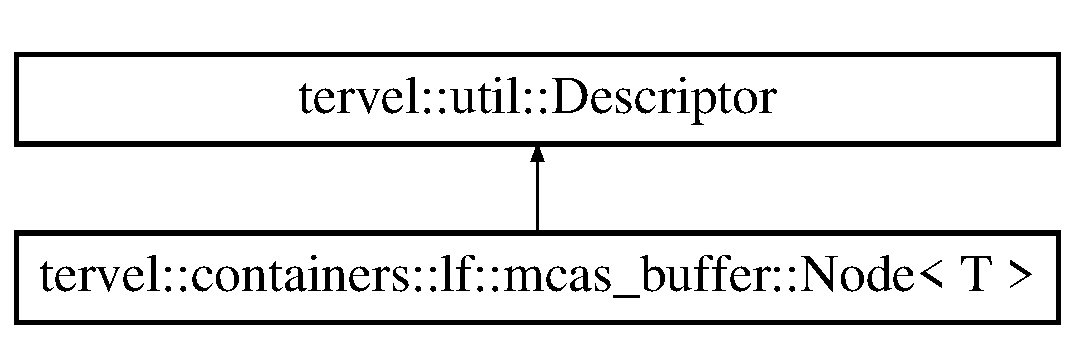
\includegraphics[height=2.000000cm]{classtervel_1_1containers_1_1lf_1_1mcas__buffer_1_1_node}
\end{center}
\end{figure}
\subsection*{Public Member Functions}
\begin{DoxyCompactItemize}
\item 
\hyperlink{classtervel_1_1containers_1_1lf_1_1mcas__buffer_1_1_node_ac5c94e003f42781fa851d8f83c860901}{Node} (T val)
\item 
\hyperlink{classtervel_1_1containers_1_1lf_1_1mcas__buffer_1_1_node_a424b975f90d6ba651c10b834837165e0}{$\sim$\+Node} ()
\item 
T \hyperlink{classtervel_1_1containers_1_1lf_1_1mcas__buffer_1_1_node_a64fc5cbefc0609a1e59f0d912808ecc8}{value} ()
\item 
void $\ast$ \hyperlink{classtervel_1_1containers_1_1lf_1_1mcas__buffer_1_1_node_afee54ad05721b9418bae358383e31f89}{complete} (void $\ast$current, std\+::atomic$<$ void $\ast$ $>$ $\ast$address)
\begin{DoxyCompactList}\small\item\em This method is implemented by each sub class and must guarantee that upon return that the descriptor no longer exists at the address it was placed. \end{DoxyCompactList}\item 
void $\ast$ \hyperlink{classtervel_1_1containers_1_1lf_1_1mcas__buffer_1_1_node_aceb3488510a25751e9055f13505a6a7d}{get\+\_\+logical\+\_\+value} ()
\begin{DoxyCompactList}\small\item\em This method is implemented by each sub class. \end{DoxyCompactList}\end{DoxyCompactItemize}
\subsection*{Private Attributes}
\begin{DoxyCompactItemize}
\item 
const T \hyperlink{classtervel_1_1containers_1_1lf_1_1mcas__buffer_1_1_node_a4e4a3009f3c6bdde1a0d55513bcfc89f}{val\+\_\+}
\end{DoxyCompactItemize}


\subsection{Constructor \& Destructor Documentation}
\hypertarget{classtervel_1_1containers_1_1lf_1_1mcas__buffer_1_1_node_ac5c94e003f42781fa851d8f83c860901}{}\index{tervel\+::containers\+::lf\+::mcas\+\_\+buffer\+::\+Node@{tervel\+::containers\+::lf\+::mcas\+\_\+buffer\+::\+Node}!Node@{Node}}
\index{Node@{Node}!tervel\+::containers\+::lf\+::mcas\+\_\+buffer\+::\+Node@{tervel\+::containers\+::lf\+::mcas\+\_\+buffer\+::\+Node}}
\subsubsection[{Node(\+T val)}]{\setlength{\rightskip}{0pt plus 5cm}template$<$typename T$>$ {\bf tervel\+::containers\+::lf\+::mcas\+\_\+buffer\+::\+Node}$<$ T $>$\+::{\bf Node} (
\begin{DoxyParamCaption}
\item[{T}]{val}
\end{DoxyParamCaption}
)\hspace{0.3cm}{\ttfamily [inline]}, {\ttfamily [explicit]}}\label{classtervel_1_1containers_1_1lf_1_1mcas__buffer_1_1_node_ac5c94e003f42781fa851d8f83c860901}
\hypertarget{classtervel_1_1containers_1_1lf_1_1mcas__buffer_1_1_node_a424b975f90d6ba651c10b834837165e0}{}\index{tervel\+::containers\+::lf\+::mcas\+\_\+buffer\+::\+Node@{tervel\+::containers\+::lf\+::mcas\+\_\+buffer\+::\+Node}!````~Node@{$\sim$\+Node}}
\index{````~Node@{$\sim$\+Node}!tervel\+::containers\+::lf\+::mcas\+\_\+buffer\+::\+Node@{tervel\+::containers\+::lf\+::mcas\+\_\+buffer\+::\+Node}}
\subsubsection[{$\sim$\+Node()}]{\setlength{\rightskip}{0pt plus 5cm}template$<$typename T$>$ {\bf tervel\+::containers\+::lf\+::mcas\+\_\+buffer\+::\+Node}$<$ T $>$\+::$\sim${\bf Node} (
\begin{DoxyParamCaption}
{}
\end{DoxyParamCaption}
)\hspace{0.3cm}{\ttfamily [inline]}}\label{classtervel_1_1containers_1_1lf_1_1mcas__buffer_1_1_node_a424b975f90d6ba651c10b834837165e0}


\subsection{Member Function Documentation}
\hypertarget{classtervel_1_1containers_1_1lf_1_1mcas__buffer_1_1_node_afee54ad05721b9418bae358383e31f89}{}\index{tervel\+::containers\+::lf\+::mcas\+\_\+buffer\+::\+Node@{tervel\+::containers\+::lf\+::mcas\+\_\+buffer\+::\+Node}!complete@{complete}}
\index{complete@{complete}!tervel\+::containers\+::lf\+::mcas\+\_\+buffer\+::\+Node@{tervel\+::containers\+::lf\+::mcas\+\_\+buffer\+::\+Node}}
\subsubsection[{complete(void $\ast$current, std\+::atomic$<$ void $\ast$ $>$ $\ast$address)}]{\setlength{\rightskip}{0pt plus 5cm}template$<$typename T$>$ void$\ast$ {\bf tervel\+::containers\+::lf\+::mcas\+\_\+buffer\+::\+Node}$<$ T $>$\+::complete (
\begin{DoxyParamCaption}
\item[{void $\ast$}]{current, }
\item[{std\+::atomic$<$ void $\ast$ $>$ $\ast$}]{address}
\end{DoxyParamCaption}
)\hspace{0.3cm}{\ttfamily [inline]}, {\ttfamily [virtual]}}\label{classtervel_1_1containers_1_1lf_1_1mcas__buffer_1_1_node_afee54ad05721b9418bae358383e31f89}


This method is implemented by each sub class and must guarantee that upon return that the descriptor no longer exists at the address it was placed. 


\begin{DoxyParams}{Parameters}
{\em current} & the reference to this object as it is at the address, \\
\hline
{\em address} & the location this object was read from \\
\hline
\end{DoxyParams}


Implements \hyperlink{classtervel_1_1util_1_1_descriptor_a4303b2a08e3ab67de5533cfb20db87c9}{tervel\+::util\+::\+Descriptor}.

\hypertarget{classtervel_1_1containers_1_1lf_1_1mcas__buffer_1_1_node_aceb3488510a25751e9055f13505a6a7d}{}\index{tervel\+::containers\+::lf\+::mcas\+\_\+buffer\+::\+Node@{tervel\+::containers\+::lf\+::mcas\+\_\+buffer\+::\+Node}!get\+\_\+logical\+\_\+value@{get\+\_\+logical\+\_\+value}}
\index{get\+\_\+logical\+\_\+value@{get\+\_\+logical\+\_\+value}!tervel\+::containers\+::lf\+::mcas\+\_\+buffer\+::\+Node@{tervel\+::containers\+::lf\+::mcas\+\_\+buffer\+::\+Node}}
\subsubsection[{get\+\_\+logical\+\_\+value()}]{\setlength{\rightskip}{0pt plus 5cm}template$<$typename T$>$ void$\ast$ {\bf tervel\+::containers\+::lf\+::mcas\+\_\+buffer\+::\+Node}$<$ T $>$\+::get\+\_\+logical\+\_\+value (
\begin{DoxyParamCaption}
{}
\end{DoxyParamCaption}
)\hspace{0.3cm}{\ttfamily [inline]}, {\ttfamily [virtual]}}\label{classtervel_1_1containers_1_1lf_1_1mcas__buffer_1_1_node_aceb3488510a25751e9055f13505a6a7d}


This method is implemented by each sub class. 

It returns the logical value of the past address. If the associated operation is still in progress then it will generally return the value that was replaced by this descriptor. Otherwise it will generally return the result of the operation for the specified address.

It can only be called from the static function which protects the object from being reused during the function. 

Implements \hyperlink{classtervel_1_1util_1_1_descriptor_a5b443eeb6acf1207f27a6d06c39d4ad4}{tervel\+::util\+::\+Descriptor}.

\hypertarget{classtervel_1_1containers_1_1lf_1_1mcas__buffer_1_1_node_a64fc5cbefc0609a1e59f0d912808ecc8}{}\index{tervel\+::containers\+::lf\+::mcas\+\_\+buffer\+::\+Node@{tervel\+::containers\+::lf\+::mcas\+\_\+buffer\+::\+Node}!value@{value}}
\index{value@{value}!tervel\+::containers\+::lf\+::mcas\+\_\+buffer\+::\+Node@{tervel\+::containers\+::lf\+::mcas\+\_\+buffer\+::\+Node}}
\subsubsection[{value()}]{\setlength{\rightskip}{0pt plus 5cm}template$<$typename T$>$ T {\bf tervel\+::containers\+::lf\+::mcas\+\_\+buffer\+::\+Node}$<$ T $>$\+::value (
\begin{DoxyParamCaption}
{}
\end{DoxyParamCaption}
)\hspace{0.3cm}{\ttfamily [inline]}}\label{classtervel_1_1containers_1_1lf_1_1mcas__buffer_1_1_node_a64fc5cbefc0609a1e59f0d912808ecc8}


\subsection{Member Data Documentation}
\hypertarget{classtervel_1_1containers_1_1lf_1_1mcas__buffer_1_1_node_a4e4a3009f3c6bdde1a0d55513bcfc89f}{}\index{tervel\+::containers\+::lf\+::mcas\+\_\+buffer\+::\+Node@{tervel\+::containers\+::lf\+::mcas\+\_\+buffer\+::\+Node}!val\+\_\+@{val\+\_\+}}
\index{val\+\_\+@{val\+\_\+}!tervel\+::containers\+::lf\+::mcas\+\_\+buffer\+::\+Node@{tervel\+::containers\+::lf\+::mcas\+\_\+buffer\+::\+Node}}
\subsubsection[{val\+\_\+}]{\setlength{\rightskip}{0pt plus 5cm}template$<$typename T$>$ const T {\bf tervel\+::containers\+::lf\+::mcas\+\_\+buffer\+::\+Node}$<$ T $>$\+::val\+\_\+\hspace{0.3cm}{\ttfamily [private]}}\label{classtervel_1_1containers_1_1lf_1_1mcas__buffer_1_1_node_a4e4a3009f3c6bdde1a0d55513bcfc89f}


The documentation for this class was generated from the following file\+:\begin{DoxyCompactItemize}
\item 
tervel/containers/lf/mcas-\/buffer/\hyperlink{mcas__buffer_8h}{mcas\+\_\+buffer.\+h}\end{DoxyCompactItemize}

\hypertarget{classtervel_1_1containers_1_1wf_1_1_hash_map_1_1_node}{}\section{tervel\+:\+:containers\+:\+:wf\+:\+:Hash\+Map$<$ Key, Value, Functor $>$\+:\+:Node Class Reference}
\label{classtervel_1_1containers_1_1wf_1_1_hash_map_1_1_node}\index{tervel\+::containers\+::wf\+::\+Hash\+Map$<$ Key, Value, Functor $>$\+::\+Node@{tervel\+::containers\+::wf\+::\+Hash\+Map$<$ Key, Value, Functor $>$\+::\+Node}}


This class is used to differentiate between data\+\_\+nodes and array\+\_\+nodes/.  


Inheritance diagram for tervel\+:\+:containers\+:\+:wf\+:\+:Hash\+Map$<$ Key, Value, Functor $>$\+:\+:Node\+:\begin{figure}[H]
\begin{center}
\leavevmode
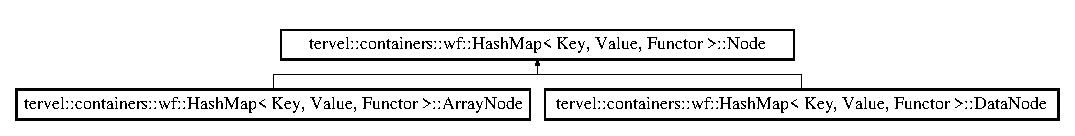
\includegraphics[height=1.379310cm]{classtervel_1_1containers_1_1wf_1_1_hash_map_1_1_node}
\end{center}
\end{figure}
\subsection*{Public Member Functions}
\begin{DoxyCompactItemize}
\item 
\hyperlink{classtervel_1_1containers_1_1wf_1_1_hash_map_1_1_node_a527126a2a9e22cce4e8ea3634168de62}{Node} ()
\item 
virtual \hyperlink{classtervel_1_1containers_1_1wf_1_1_hash_map_1_1_node_aa9a636d0614e3bb54e81543027558a08}{$\sim$\+Node} ()
\item 
virtual bool \hyperlink{classtervel_1_1containers_1_1wf_1_1_hash_map_1_1_node_a0908bd3151f0b1b7f8fbb6825731fd15}{is\+\_\+array} ()=0
\item 
virtual bool \hyperlink{classtervel_1_1containers_1_1wf_1_1_hash_map_1_1_node_ac7cc7039cfc134def7d936f00efc2155}{is\+\_\+data} ()=0
\end{DoxyCompactItemize}


\subsection{Detailed Description}
\subsubsection*{template$<$class Key, class Value, class Functor = default\+\_\+functor$<$\+Key, Value$>$$>$class tervel\+::containers\+::wf\+::\+Hash\+Map$<$ Key, Value, Functor $>$\+::\+Node}

This class is used to differentiate between data\+\_\+nodes and array\+\_\+nodes/. 

\subsection{Constructor \& Destructor Documentation}
\hypertarget{classtervel_1_1containers_1_1wf_1_1_hash_map_1_1_node_a527126a2a9e22cce4e8ea3634168de62}{}\index{tervel\+::containers\+::wf\+::\+Hash\+Map\+::\+Node@{tervel\+::containers\+::wf\+::\+Hash\+Map\+::\+Node}!Node@{Node}}
\index{Node@{Node}!tervel\+::containers\+::wf\+::\+Hash\+Map\+::\+Node@{tervel\+::containers\+::wf\+::\+Hash\+Map\+::\+Node}}
\subsubsection[{Node()}]{\setlength{\rightskip}{0pt plus 5cm}template$<$class Key , class Value , class Functor  = default\+\_\+functor$<$\+Key, Value$>$$>$ {\bf tervel\+::containers\+::wf\+::\+Hash\+Map}$<$ Key, {\bf Value}, Functor $>$\+::Node\+::\+Node (
\begin{DoxyParamCaption}
{}
\end{DoxyParamCaption}
)\hspace{0.3cm}{\ttfamily [inline]}}\label{classtervel_1_1containers_1_1wf_1_1_hash_map_1_1_node_a527126a2a9e22cce4e8ea3634168de62}
\hypertarget{classtervel_1_1containers_1_1wf_1_1_hash_map_1_1_node_aa9a636d0614e3bb54e81543027558a08}{}\index{tervel\+::containers\+::wf\+::\+Hash\+Map\+::\+Node@{tervel\+::containers\+::wf\+::\+Hash\+Map\+::\+Node}!````~Node@{$\sim$\+Node}}
\index{````~Node@{$\sim$\+Node}!tervel\+::containers\+::wf\+::\+Hash\+Map\+::\+Node@{tervel\+::containers\+::wf\+::\+Hash\+Map\+::\+Node}}
\subsubsection[{$\sim$\+Node()}]{\setlength{\rightskip}{0pt plus 5cm}template$<$class Key , class Value , class Functor  = default\+\_\+functor$<$\+Key, Value$>$$>$ virtual {\bf tervel\+::containers\+::wf\+::\+Hash\+Map}$<$ Key, {\bf Value}, Functor $>$\+::Node\+::$\sim$\+Node (
\begin{DoxyParamCaption}
{}
\end{DoxyParamCaption}
)\hspace{0.3cm}{\ttfamily [inline]}, {\ttfamily [virtual]}}\label{classtervel_1_1containers_1_1wf_1_1_hash_map_1_1_node_aa9a636d0614e3bb54e81543027558a08}


\subsection{Member Function Documentation}
\hypertarget{classtervel_1_1containers_1_1wf_1_1_hash_map_1_1_node_a0908bd3151f0b1b7f8fbb6825731fd15}{}\index{tervel\+::containers\+::wf\+::\+Hash\+Map\+::\+Node@{tervel\+::containers\+::wf\+::\+Hash\+Map\+::\+Node}!is\+\_\+array@{is\+\_\+array}}
\index{is\+\_\+array@{is\+\_\+array}!tervel\+::containers\+::wf\+::\+Hash\+Map\+::\+Node@{tervel\+::containers\+::wf\+::\+Hash\+Map\+::\+Node}}
\subsubsection[{is\+\_\+array()=0}]{\setlength{\rightskip}{0pt plus 5cm}template$<$class Key , class Value , class Functor  = default\+\_\+functor$<$\+Key, Value$>$$>$ virtual bool {\bf tervel\+::containers\+::wf\+::\+Hash\+Map}$<$ Key, {\bf Value}, Functor $>$\+::Node\+::is\+\_\+array (
\begin{DoxyParamCaption}
{}
\end{DoxyParamCaption}
)\hspace{0.3cm}{\ttfamily [pure virtual]}}\label{classtervel_1_1containers_1_1wf_1_1_hash_map_1_1_node_a0908bd3151f0b1b7f8fbb6825731fd15}
\begin{DoxyReturn}{Returns}
whether or not this instance is an \hyperlink{classtervel_1_1containers_1_1wf_1_1_hash_map_1_1_array_node}{Array\+Node} sub type 
\end{DoxyReturn}


Implemented in \hyperlink{classtervel_1_1containers_1_1wf_1_1_hash_map_1_1_data_node_a3b607ee5aaa378bd16f398c11708769e}{tervel\+::containers\+::wf\+::\+Hash\+Map$<$ Key, Value, Functor $>$\+::\+Data\+Node}, and \hyperlink{classtervel_1_1containers_1_1wf_1_1_hash_map_1_1_array_node_ad5eeaa33f2410902fbd86083e24730ca}{tervel\+::containers\+::wf\+::\+Hash\+Map$<$ Key, Value, Functor $>$\+::\+Array\+Node}.

\hypertarget{classtervel_1_1containers_1_1wf_1_1_hash_map_1_1_node_ac7cc7039cfc134def7d936f00efc2155}{}\index{tervel\+::containers\+::wf\+::\+Hash\+Map\+::\+Node@{tervel\+::containers\+::wf\+::\+Hash\+Map\+::\+Node}!is\+\_\+data@{is\+\_\+data}}
\index{is\+\_\+data@{is\+\_\+data}!tervel\+::containers\+::wf\+::\+Hash\+Map\+::\+Node@{tervel\+::containers\+::wf\+::\+Hash\+Map\+::\+Node}}
\subsubsection[{is\+\_\+data()=0}]{\setlength{\rightskip}{0pt plus 5cm}template$<$class Key , class Value , class Functor  = default\+\_\+functor$<$\+Key, Value$>$$>$ virtual bool {\bf tervel\+::containers\+::wf\+::\+Hash\+Map}$<$ Key, {\bf Value}, Functor $>$\+::Node\+::is\+\_\+data (
\begin{DoxyParamCaption}
{}
\end{DoxyParamCaption}
)\hspace{0.3cm}{\ttfamily [pure virtual]}}\label{classtervel_1_1containers_1_1wf_1_1_hash_map_1_1_node_ac7cc7039cfc134def7d936f00efc2155}
\begin{DoxyReturn}{Returns}
whether or not this instance is an \hyperlink{classtervel_1_1containers_1_1wf_1_1_hash_map_1_1_data_node}{Data\+Node} sub type 
\end{DoxyReturn}


Implemented in \hyperlink{classtervel_1_1containers_1_1wf_1_1_hash_map_1_1_data_node_a4a5c4a7e2de1b689d515d8d97322599d}{tervel\+::containers\+::wf\+::\+Hash\+Map$<$ Key, Value, Functor $>$\+::\+Data\+Node}, and \hyperlink{classtervel_1_1containers_1_1wf_1_1_hash_map_1_1_array_node_a21681cf8d295b98084b1bebc5e434a7d}{tervel\+::containers\+::wf\+::\+Hash\+Map$<$ Key, Value, Functor $>$\+::\+Array\+Node}.



The documentation for this class was generated from the following file\+:\begin{DoxyCompactItemize}
\item 
tervel/containers/wf/hash-\/map/\hyperlink{wf__hash__map_8h}{wf\+\_\+hash\+\_\+map.\+h}\end{DoxyCompactItemize}

\hypertarget{classtervel_1_1containers_1_1wf_1_1_hash_map_no_delete_1_1_node}{}\section{tervel\+:\+:containers\+:\+:wf\+:\+:Hash\+Map\+No\+Delete$<$ Key, Value, Functor $>$\+:\+:Node Class Reference}
\label{classtervel_1_1containers_1_1wf_1_1_hash_map_no_delete_1_1_node}\index{tervel\+::containers\+::wf\+::\+Hash\+Map\+No\+Delete$<$ Key, Value, Functor $>$\+::\+Node@{tervel\+::containers\+::wf\+::\+Hash\+Map\+No\+Delete$<$ Key, Value, Functor $>$\+::\+Node}}


This class is used to differentiate between data\+\_\+nodes and array\+\_\+nodes/.  


Inheritance diagram for tervel\+:\+:containers\+:\+:wf\+:\+:Hash\+Map\+No\+Delete$<$ Key, Value, Functor $>$\+:\+:Node\+:\begin{figure}[H]
\begin{center}
\leavevmode
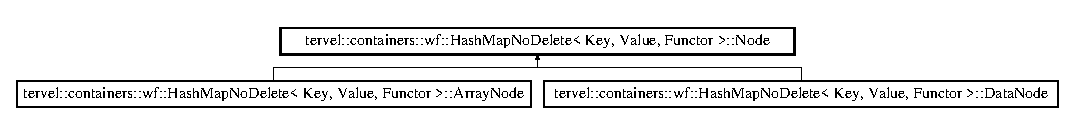
\includegraphics[height=1.222707cm]{classtervel_1_1containers_1_1wf_1_1_hash_map_no_delete_1_1_node}
\end{center}
\end{figure}
\subsection*{Public Member Functions}
\begin{DoxyCompactItemize}
\item 
\hyperlink{classtervel_1_1containers_1_1wf_1_1_hash_map_no_delete_1_1_node_ad277ea9a398c9bf518b986fdd7efd46e}{Node} ()
\item 
virtual \hyperlink{classtervel_1_1containers_1_1wf_1_1_hash_map_no_delete_1_1_node_a7f65753fac9617b5e9cb072d31131f52}{$\sim$\+Node} ()
\item 
virtual bool \hyperlink{classtervel_1_1containers_1_1wf_1_1_hash_map_no_delete_1_1_node_a551c6b4900b06efe3fc1d4de7c25963b}{is\+\_\+array} ()=0
\item 
virtual bool \hyperlink{classtervel_1_1containers_1_1wf_1_1_hash_map_no_delete_1_1_node_a03ef6395f93104d0313296773be36b3c}{is\+\_\+data} ()=0
\end{DoxyCompactItemize}


\subsection{Detailed Description}
\subsubsection*{template$<$class Key, class Value, class Functor = default\+\_\+functor$<$\+Key, Value$>$$>$class tervel\+::containers\+::wf\+::\+Hash\+Map\+No\+Delete$<$ Key, Value, Functor $>$\+::\+Node}

This class is used to differentiate between data\+\_\+nodes and array\+\_\+nodes/. 

\subsection{Constructor \& Destructor Documentation}
\hypertarget{classtervel_1_1containers_1_1wf_1_1_hash_map_no_delete_1_1_node_ad277ea9a398c9bf518b986fdd7efd46e}{}\index{tervel\+::containers\+::wf\+::\+Hash\+Map\+No\+Delete\+::\+Node@{tervel\+::containers\+::wf\+::\+Hash\+Map\+No\+Delete\+::\+Node}!Node@{Node}}
\index{Node@{Node}!tervel\+::containers\+::wf\+::\+Hash\+Map\+No\+Delete\+::\+Node@{tervel\+::containers\+::wf\+::\+Hash\+Map\+No\+Delete\+::\+Node}}
\subsubsection[{Node()}]{\setlength{\rightskip}{0pt plus 5cm}template$<$class Key , class Value , class Functor  = default\+\_\+functor$<$\+Key, Value$>$$>$ {\bf tervel\+::containers\+::wf\+::\+Hash\+Map\+No\+Delete}$<$ Key, {\bf Value}, Functor $>$\+::Node\+::\+Node (
\begin{DoxyParamCaption}
{}
\end{DoxyParamCaption}
)\hspace{0.3cm}{\ttfamily [inline]}}\label{classtervel_1_1containers_1_1wf_1_1_hash_map_no_delete_1_1_node_ad277ea9a398c9bf518b986fdd7efd46e}
\hypertarget{classtervel_1_1containers_1_1wf_1_1_hash_map_no_delete_1_1_node_a7f65753fac9617b5e9cb072d31131f52}{}\index{tervel\+::containers\+::wf\+::\+Hash\+Map\+No\+Delete\+::\+Node@{tervel\+::containers\+::wf\+::\+Hash\+Map\+No\+Delete\+::\+Node}!````~Node@{$\sim$\+Node}}
\index{````~Node@{$\sim$\+Node}!tervel\+::containers\+::wf\+::\+Hash\+Map\+No\+Delete\+::\+Node@{tervel\+::containers\+::wf\+::\+Hash\+Map\+No\+Delete\+::\+Node}}
\subsubsection[{$\sim$\+Node()}]{\setlength{\rightskip}{0pt plus 5cm}template$<$class Key , class Value , class Functor  = default\+\_\+functor$<$\+Key, Value$>$$>$ virtual {\bf tervel\+::containers\+::wf\+::\+Hash\+Map\+No\+Delete}$<$ Key, {\bf Value}, Functor $>$\+::Node\+::$\sim$\+Node (
\begin{DoxyParamCaption}
{}
\end{DoxyParamCaption}
)\hspace{0.3cm}{\ttfamily [inline]}, {\ttfamily [virtual]}}\label{classtervel_1_1containers_1_1wf_1_1_hash_map_no_delete_1_1_node_a7f65753fac9617b5e9cb072d31131f52}


\subsection{Member Function Documentation}
\hypertarget{classtervel_1_1containers_1_1wf_1_1_hash_map_no_delete_1_1_node_a551c6b4900b06efe3fc1d4de7c25963b}{}\index{tervel\+::containers\+::wf\+::\+Hash\+Map\+No\+Delete\+::\+Node@{tervel\+::containers\+::wf\+::\+Hash\+Map\+No\+Delete\+::\+Node}!is\+\_\+array@{is\+\_\+array}}
\index{is\+\_\+array@{is\+\_\+array}!tervel\+::containers\+::wf\+::\+Hash\+Map\+No\+Delete\+::\+Node@{tervel\+::containers\+::wf\+::\+Hash\+Map\+No\+Delete\+::\+Node}}
\subsubsection[{is\+\_\+array()=0}]{\setlength{\rightskip}{0pt plus 5cm}template$<$class Key , class Value , class Functor  = default\+\_\+functor$<$\+Key, Value$>$$>$ virtual bool {\bf tervel\+::containers\+::wf\+::\+Hash\+Map\+No\+Delete}$<$ Key, {\bf Value}, Functor $>$\+::Node\+::is\+\_\+array (
\begin{DoxyParamCaption}
{}
\end{DoxyParamCaption}
)\hspace{0.3cm}{\ttfamily [pure virtual]}}\label{classtervel_1_1containers_1_1wf_1_1_hash_map_no_delete_1_1_node_a551c6b4900b06efe3fc1d4de7c25963b}
\begin{DoxyReturn}{Returns}
whether or not this instance is an \hyperlink{classtervel_1_1containers_1_1wf_1_1_hash_map_no_delete_1_1_array_node}{Array\+Node} sub type 
\end{DoxyReturn}


Implemented in \hyperlink{classtervel_1_1containers_1_1wf_1_1_hash_map_no_delete_1_1_data_node_a12ef4de7bec0bb237d2cb4f3eeab1a7d}{tervel\+::containers\+::wf\+::\+Hash\+Map\+No\+Delete$<$ Key, Value, Functor $>$\+::\+Data\+Node}, and \hyperlink{classtervel_1_1containers_1_1wf_1_1_hash_map_no_delete_1_1_array_node_a11f011931040dfd98938b073006cb04b}{tervel\+::containers\+::wf\+::\+Hash\+Map\+No\+Delete$<$ Key, Value, Functor $>$\+::\+Array\+Node}.

\hypertarget{classtervel_1_1containers_1_1wf_1_1_hash_map_no_delete_1_1_node_a03ef6395f93104d0313296773be36b3c}{}\index{tervel\+::containers\+::wf\+::\+Hash\+Map\+No\+Delete\+::\+Node@{tervel\+::containers\+::wf\+::\+Hash\+Map\+No\+Delete\+::\+Node}!is\+\_\+data@{is\+\_\+data}}
\index{is\+\_\+data@{is\+\_\+data}!tervel\+::containers\+::wf\+::\+Hash\+Map\+No\+Delete\+::\+Node@{tervel\+::containers\+::wf\+::\+Hash\+Map\+No\+Delete\+::\+Node}}
\subsubsection[{is\+\_\+data()=0}]{\setlength{\rightskip}{0pt plus 5cm}template$<$class Key , class Value , class Functor  = default\+\_\+functor$<$\+Key, Value$>$$>$ virtual bool {\bf tervel\+::containers\+::wf\+::\+Hash\+Map\+No\+Delete}$<$ Key, {\bf Value}, Functor $>$\+::Node\+::is\+\_\+data (
\begin{DoxyParamCaption}
{}
\end{DoxyParamCaption}
)\hspace{0.3cm}{\ttfamily [pure virtual]}}\label{classtervel_1_1containers_1_1wf_1_1_hash_map_no_delete_1_1_node_a03ef6395f93104d0313296773be36b3c}
\begin{DoxyReturn}{Returns}
whether or not this instance is an \hyperlink{classtervel_1_1containers_1_1wf_1_1_hash_map_no_delete_1_1_data_node}{Data\+Node} sub type 
\end{DoxyReturn}


Implemented in \hyperlink{classtervel_1_1containers_1_1wf_1_1_hash_map_no_delete_1_1_data_node_af8b10e3d6d939fd4655e92b884b160cf}{tervel\+::containers\+::wf\+::\+Hash\+Map\+No\+Delete$<$ Key, Value, Functor $>$\+::\+Data\+Node}, and \hyperlink{classtervel_1_1containers_1_1wf_1_1_hash_map_no_delete_1_1_array_node_a049ba7f928ab0c87be2e0466f8d29a1b}{tervel\+::containers\+::wf\+::\+Hash\+Map\+No\+Delete$<$ Key, Value, Functor $>$\+::\+Array\+Node}.



The documentation for this class was generated from the following file\+:\begin{DoxyCompactItemize}
\item 
tervel/containers/wf/hash-\/map/\hyperlink{wf__hash__map__no__delete_8h}{wf\+\_\+hash\+\_\+map\+\_\+no\+\_\+delete.\+h}\end{DoxyCompactItemize}

\hypertarget{classtervel_1_1util_1_1_op_record}{}\section{tervel\+:\+:util\+:\+:Op\+Record Class Reference}
\label{classtervel_1_1util_1_1_op_record}\index{tervel\+::util\+::\+Op\+Record@{tervel\+::util\+::\+Op\+Record}}


This class is used to create Operation Records.  




{\ttfamily \#include $<$progress\+\_\+assurance.\+h$>$}

Inheritance diagram for tervel\+:\+:util\+:\+:Op\+Record\+:\begin{figure}[H]
\begin{center}
\leavevmode
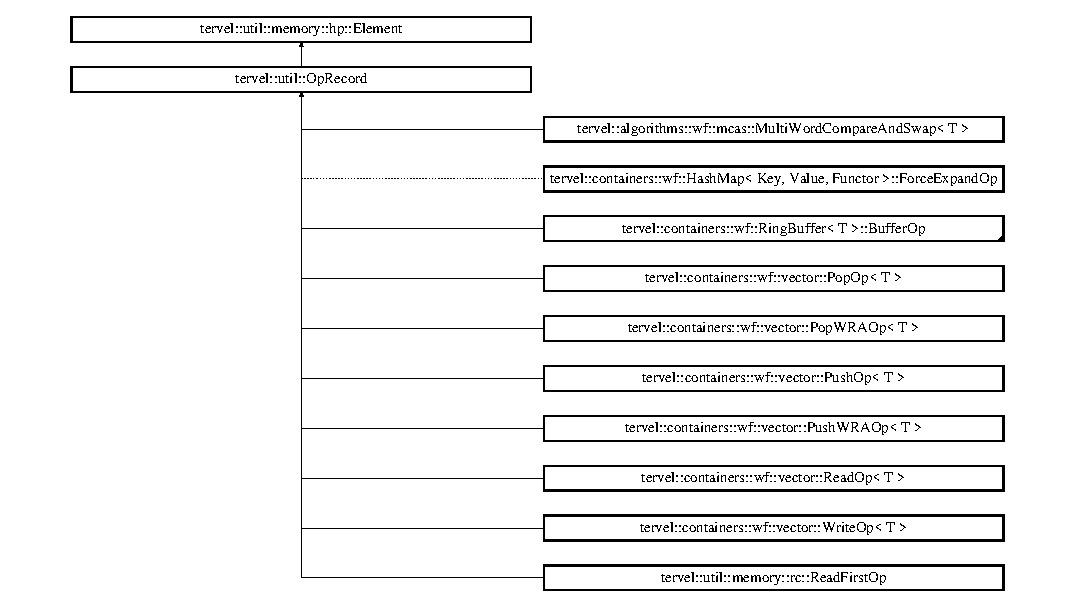
\includegraphics[height=7.706422cm]{classtervel_1_1util_1_1_op_record}
\end{center}
\end{figure}
\subsection*{Public Member Functions}
\begin{DoxyCompactItemize}
\item 
\hyperlink{classtervel_1_1util_1_1_op_record_aab6cd47463ff94ff4e94a7f1a57b7312}{Op\+Record} ()
\item 
virtual void \hyperlink{classtervel_1_1util_1_1_op_record_aa75ab39688a8d4cceb6a1ef0409537c0}{help\+\_\+complete} ()=0
\begin{DoxyCompactList}\small\item\em Implementations of this function that upon its return the operation described in the \hyperlink{classtervel_1_1util_1_1_op_record}{Op\+Record} has been completed. \end{DoxyCompactList}\item 
bool \hyperlink{classtervel_1_1util_1_1_op_record_a6433f4d6d353ba6ed66e8eaefaa07d32}{on\+\_\+watch} (std\+::atomic$<$ void $\ast$ $>$ $\ast$address, void $\ast$expected)
\begin{DoxyCompactList}\small\item\em This function is used to achieve a strong watch on an Element. \end{DoxyCompactList}\item 
bool \hyperlink{classtervel_1_1util_1_1_op_record_a80c4ee47bebf246ce40bb922958dd21b}{on\+\_\+is\+\_\+watched} ()
\begin{DoxyCompactList}\small\item\em This function is used to check a strong watch on an Element. \end{DoxyCompactList}\item 
void \hyperlink{classtervel_1_1util_1_1_op_record_a0018d1a71b9b3dcc4e2f59f34c938a46}{on\+\_\+unwatch} ()
\begin{DoxyCompactList}\small\item\em This function is used to remove a strong watch on an Element. \end{DoxyCompactList}\end{DoxyCompactItemize}
\subsection*{Private Member Functions}
\begin{DoxyCompactItemize}
\item 
\hyperlink{classtervel_1_1util_1_1_op_record_abf951d0ffac66bfebc8ae6aef8a3c6e1}{D\+I\+S\+A\+L\+L\+O\+W\+\_\+\+C\+O\+P\+Y\+\_\+\+A\+N\+D\+\_\+\+A\+S\+S\+I\+G\+N} (\hyperlink{classtervel_1_1util_1_1_op_record}{Op\+Record})
\end{DoxyCompactItemize}


\subsection{Detailed Description}
This class is used to create Operation Records. 

Operation records are designed to allow an arbitary thread to complete some other thread\textquotesingle{}s operation in the event that thread is unable to do so. These objects are H\+P protected. 

\subsection{Constructor \& Destructor Documentation}
\hypertarget{classtervel_1_1util_1_1_op_record_aab6cd47463ff94ff4e94a7f1a57b7312}{}\index{tervel\+::util\+::\+Op\+Record@{tervel\+::util\+::\+Op\+Record}!Op\+Record@{Op\+Record}}
\index{Op\+Record@{Op\+Record}!tervel\+::util\+::\+Op\+Record@{tervel\+::util\+::\+Op\+Record}}
\subsubsection[{Op\+Record()}]{\setlength{\rightskip}{0pt plus 5cm}tervel\+::util\+::\+Op\+Record\+::\+Op\+Record (
\begin{DoxyParamCaption}
{}
\end{DoxyParamCaption}
)\hspace{0.3cm}{\ttfamily [inline]}}\label{classtervel_1_1util_1_1_op_record_aab6cd47463ff94ff4e94a7f1a57b7312}


\subsection{Member Function Documentation}
\hypertarget{classtervel_1_1util_1_1_op_record_abf951d0ffac66bfebc8ae6aef8a3c6e1}{}\index{tervel\+::util\+::\+Op\+Record@{tervel\+::util\+::\+Op\+Record}!D\+I\+S\+A\+L\+L\+O\+W\+\_\+\+C\+O\+P\+Y\+\_\+\+A\+N\+D\+\_\+\+A\+S\+S\+I\+G\+N@{D\+I\+S\+A\+L\+L\+O\+W\+\_\+\+C\+O\+P\+Y\+\_\+\+A\+N\+D\+\_\+\+A\+S\+S\+I\+G\+N}}
\index{D\+I\+S\+A\+L\+L\+O\+W\+\_\+\+C\+O\+P\+Y\+\_\+\+A\+N\+D\+\_\+\+A\+S\+S\+I\+G\+N@{D\+I\+S\+A\+L\+L\+O\+W\+\_\+\+C\+O\+P\+Y\+\_\+\+A\+N\+D\+\_\+\+A\+S\+S\+I\+G\+N}!tervel\+::util\+::\+Op\+Record@{tervel\+::util\+::\+Op\+Record}}
\subsubsection[{D\+I\+S\+A\+L\+L\+O\+W\+\_\+\+C\+O\+P\+Y\+\_\+\+A\+N\+D\+\_\+\+A\+S\+S\+I\+G\+N(\+Op\+Record)}]{\setlength{\rightskip}{0pt plus 5cm}tervel\+::util\+::\+Op\+Record\+::\+D\+I\+S\+A\+L\+L\+O\+W\+\_\+\+C\+O\+P\+Y\+\_\+\+A\+N\+D\+\_\+\+A\+S\+S\+I\+G\+N (
\begin{DoxyParamCaption}
\item[{{\bf Op\+Record}}]{}
\end{DoxyParamCaption}
)\hspace{0.3cm}{\ttfamily [private]}}\label{classtervel_1_1util_1_1_op_record_abf951d0ffac66bfebc8ae6aef8a3c6e1}
\hypertarget{classtervel_1_1util_1_1_op_record_aa75ab39688a8d4cceb6a1ef0409537c0}{}\index{tervel\+::util\+::\+Op\+Record@{tervel\+::util\+::\+Op\+Record}!help\+\_\+complete@{help\+\_\+complete}}
\index{help\+\_\+complete@{help\+\_\+complete}!tervel\+::util\+::\+Op\+Record@{tervel\+::util\+::\+Op\+Record}}
\subsubsection[{help\+\_\+complete()=0}]{\setlength{\rightskip}{0pt plus 5cm}virtual void tervel\+::util\+::\+Op\+Record\+::help\+\_\+complete (
\begin{DoxyParamCaption}
{}
\end{DoxyParamCaption}
)\hspace{0.3cm}{\ttfamily [pure virtual]}}\label{classtervel_1_1util_1_1_op_record_aa75ab39688a8d4cceb6a1ef0409537c0}


Implementations of this function that upon its return the operation described in the \hyperlink{classtervel_1_1util_1_1_op_record}{Op\+Record} has been completed. 

As such it must be thread-\/safe and the extending class must contain all the information necessary to complete the operation. 

Implemented in \hyperlink{classtervel_1_1containers_1_1wf_1_1_hash_map_1_1_force_expand_op_adfe48adab3158c1e81119a2ff369e3d8}{tervel\+::containers\+::wf\+::\+Hash\+Map$<$ Key, Value, Functor $>$\+::\+Force\+Expand\+Op}, \hyperlink{classtervel_1_1containers_1_1wf_1_1vector_1_1_pop_op_abd820a976a7f356f87ed8dadddef12c4}{tervel\+::containers\+::wf\+::vector\+::\+Pop\+Op$<$ T $>$}, \hyperlink{classtervel_1_1containers_1_1wf_1_1vector_1_1_push_op_aca23a90c8ef1a6ac95a102def3b63d56}{tervel\+::containers\+::wf\+::vector\+::\+Push\+Op$<$ T $>$}, \hyperlink{classtervel_1_1algorithms_1_1wf_1_1mcas_1_1_multi_word_compare_and_swap_a2581e26f73e07c80473cf2999cf45652}{tervel\+::algorithms\+::wf\+::mcas\+::\+Multi\+Word\+Compare\+And\+Swap$<$ T $>$}, \hyperlink{classtervel_1_1containers_1_1wf_1_1vector_1_1_pop_w_r_a_op_ab9dbcb928b3805f777856e2e35e9b461}{tervel\+::containers\+::wf\+::vector\+::\+Pop\+W\+R\+A\+Op$<$ T $>$}, \hyperlink{classtervel_1_1containers_1_1wf_1_1vector_1_1_write_op_a30f4a6d0e37b6e591fb986977304e08d}{tervel\+::containers\+::wf\+::vector\+::\+Write\+Op$<$ T $>$}, \hyperlink{classtervel_1_1containers_1_1wf_1_1vector_1_1_push_w_r_a_op_ae06dc17442f24775407ce7eabbf79a59}{tervel\+::containers\+::wf\+::vector\+::\+Push\+W\+R\+A\+Op$<$ T $>$}, \hyperlink{classtervel_1_1util_1_1memory_1_1rc_1_1_read_first_op_a21e1fa517b7e7f522be78dcc95d810da}{tervel\+::util\+::memory\+::rc\+::\+Read\+First\+Op}, \hyperlink{classtervel_1_1containers_1_1wf_1_1_ring_buffer_1_1_enqueue_op_a928f562593a93be6c99df05c128012b8}{tervel\+::containers\+::wf\+::\+Ring\+Buffer$<$ T $>$\+::\+Enqueue\+Op$<$ T $>$}, \hyperlink{classtervel_1_1containers_1_1wf_1_1vector_1_1_read_op_ad2c5f63b0c39e1b30350656fcdd44538}{tervel\+::containers\+::wf\+::vector\+::\+Read\+Op$<$ T $>$}, and \hyperlink{classtervel_1_1containers_1_1wf_1_1_ring_buffer_1_1_dequeue_op_a0f798edd2a65caf9ce112b496c27bdd5}{tervel\+::containers\+::wf\+::\+Ring\+Buffer$<$ T $>$\+::\+Dequeue\+Op$<$ T $>$}.

\hypertarget{classtervel_1_1util_1_1_op_record_a80c4ee47bebf246ce40bb922958dd21b}{}\index{tervel\+::util\+::\+Op\+Record@{tervel\+::util\+::\+Op\+Record}!on\+\_\+is\+\_\+watched@{on\+\_\+is\+\_\+watched}}
\index{on\+\_\+is\+\_\+watched@{on\+\_\+is\+\_\+watched}!tervel\+::util\+::\+Op\+Record@{tervel\+::util\+::\+Op\+Record}}
\subsubsection[{on\+\_\+is\+\_\+watched()}]{\setlength{\rightskip}{0pt plus 5cm}bool tervel\+::util\+::\+Op\+Record\+::on\+\_\+is\+\_\+watched (
\begin{DoxyParamCaption}
{}
\end{DoxyParamCaption}
)\hspace{0.3cm}{\ttfamily [inline]}, {\ttfamily [virtual]}}\label{classtervel_1_1util_1_1_op_record_a80c4ee47bebf246ce40bb922958dd21b}


This function is used to check a strong watch on an Element. 

Classes wishing to express this should override this function.

\begin{DoxyReturn}{Returns}
whether or not the element is watched. 
\end{DoxyReturn}


Reimplemented from \hyperlink{classtervel_1_1util_1_1memory_1_1hp_1_1_element_a88306bc6b64d0110e3ee568514dbcc04}{tervel\+::util\+::memory\+::hp\+::\+Element}.

\hypertarget{classtervel_1_1util_1_1_op_record_a0018d1a71b9b3dcc4e2f59f34c938a46}{}\index{tervel\+::util\+::\+Op\+Record@{tervel\+::util\+::\+Op\+Record}!on\+\_\+unwatch@{on\+\_\+unwatch}}
\index{on\+\_\+unwatch@{on\+\_\+unwatch}!tervel\+::util\+::\+Op\+Record@{tervel\+::util\+::\+Op\+Record}}
\subsubsection[{on\+\_\+unwatch()}]{\setlength{\rightskip}{0pt plus 5cm}void tervel\+::util\+::\+Op\+Record\+::on\+\_\+unwatch (
\begin{DoxyParamCaption}
{}
\end{DoxyParamCaption}
)\hspace{0.3cm}{\ttfamily [inline]}, {\ttfamily [virtual]}}\label{classtervel_1_1util_1_1_op_record_a0018d1a71b9b3dcc4e2f59f34c938a46}


This function is used to remove a strong watch on an Element. 

Classes wishing to express this should override this function. 

Reimplemented from \hyperlink{classtervel_1_1util_1_1memory_1_1hp_1_1_element_ae71f306b6c9f08565e61546a0dc0a30c}{tervel\+::util\+::memory\+::hp\+::\+Element}.

\hypertarget{classtervel_1_1util_1_1_op_record_a6433f4d6d353ba6ed66e8eaefaa07d32}{}\index{tervel\+::util\+::\+Op\+Record@{tervel\+::util\+::\+Op\+Record}!on\+\_\+watch@{on\+\_\+watch}}
\index{on\+\_\+watch@{on\+\_\+watch}!tervel\+::util\+::\+Op\+Record@{tervel\+::util\+::\+Op\+Record}}
\subsubsection[{on\+\_\+watch(std\+::atomic$<$ void $\ast$ $>$ $\ast$address, void $\ast$expected)}]{\setlength{\rightskip}{0pt plus 5cm}bool tervel\+::util\+::\+Op\+Record\+::on\+\_\+watch (
\begin{DoxyParamCaption}
\item[{std\+::atomic$<$ void $\ast$ $>$ $\ast$}]{address, }
\item[{void $\ast$}]{expected}
\end{DoxyParamCaption}
)\hspace{0.3cm}{\ttfamily [inline]}, {\ttfamily [virtual]}}\label{classtervel_1_1util_1_1_op_record_a6433f4d6d353ba6ed66e8eaefaa07d32}


This function is used to achieve a strong watch on an Element. 

Classes wishing to express this should override this function.


\begin{DoxyParams}{Parameters}
{\em address} & the expected was load from \\
\hline
{\em expected} & the last known value of address \\
\hline
\end{DoxyParams}
\begin{DoxyReturn}{Returns}
whether or not the element was succefully watched. 
\end{DoxyReturn}


Reimplemented from \hyperlink{classtervel_1_1util_1_1memory_1_1hp_1_1_element_a53493ef4754dd77016139863af964f90}{tervel\+::util\+::memory\+::hp\+::\+Element}.



The documentation for this class was generated from the following file\+:\begin{DoxyCompactItemize}
\item 
tervel/util/\hyperlink{progress__assurance_8h}{progress\+\_\+assurance.\+h}\end{DoxyCompactItemize}

\hypertarget{struct_test_class_1_1foo__set__traits_1_1ordered__list__traits}{}\section{Test\+Class$<$ Key, Value $>$\+:\+:foo\+\_\+set\+\_\+traits\+:\+:ordered\+\_\+list\+\_\+traits Struct Reference}
\label{struct_test_class_1_1foo__set__traits_1_1ordered__list__traits}\index{Test\+Class$<$ Key, Value $>$\+::foo\+\_\+set\+\_\+traits\+::ordered\+\_\+list\+\_\+traits@{Test\+Class$<$ Key, Value $>$\+::foo\+\_\+set\+\_\+traits\+::ordered\+\_\+list\+\_\+traits}}


{\ttfamily \#include $<$cds\+\_\+split\+\_\+map.\+h$>$}

Inheritance diagram for Test\+Class$<$ Key, Value $>$\+:\+:foo\+\_\+set\+\_\+traits\+:\+:ordered\+\_\+list\+\_\+traits\+:\begin{figure}[H]
\begin{center}
\leavevmode
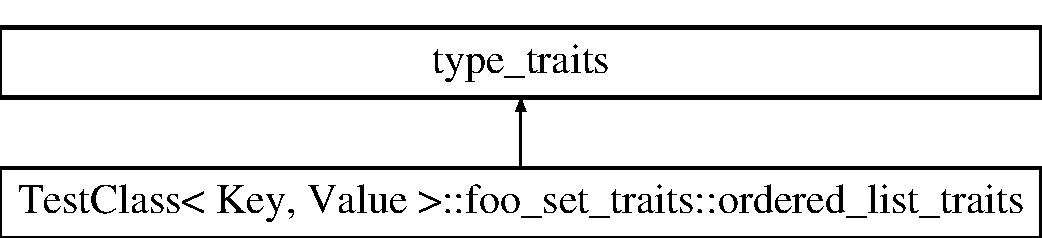
\includegraphics[height=2.000000cm]{struct_test_class_1_1foo__set__traits_1_1ordered__list__traits}
\end{center}
\end{figure}
\subsection*{Public Types}
\begin{DoxyCompactItemize}
\item 
typedef struct \hyperlink{struct_test_class_1_1less__s}{less\+\_\+s}$<$ Key $>$ \hyperlink{struct_test_class_1_1foo__set__traits_1_1ordered__list__traits_ac8741038df1d94768fbc5f5411320a1a}{less}
\end{DoxyCompactItemize}


\subsection{Member Typedef Documentation}
\hypertarget{struct_test_class_1_1foo__set__traits_1_1ordered__list__traits_ac8741038df1d94768fbc5f5411320a1a}{}\index{Test\+Class\+::foo\+\_\+set\+\_\+traits\+::ordered\+\_\+list\+\_\+traits@{Test\+Class\+::foo\+\_\+set\+\_\+traits\+::ordered\+\_\+list\+\_\+traits}!less@{less}}
\index{less@{less}!Test\+Class\+::foo\+\_\+set\+\_\+traits\+::ordered\+\_\+list\+\_\+traits@{Test\+Class\+::foo\+\_\+set\+\_\+traits\+::ordered\+\_\+list\+\_\+traits}}
\subsubsection[{less}]{\setlength{\rightskip}{0pt plus 5cm}template$<$class Key, class Value$>$ typedef struct {\bf less\+\_\+s}$<$ Key $>$ {\bf Test\+Class}$<$ Key, {\bf Value} $>$\+::{\bf foo\+\_\+set\+\_\+traits\+::ordered\+\_\+list\+\_\+traits\+::less}}\label{struct_test_class_1_1foo__set__traits_1_1ordered__list__traits_ac8741038df1d94768fbc5f5411320a1a}


The documentation for this struct was generated from the following file\+:\begin{DoxyCompactItemize}
\item 
tervel/tests/hash\+\_\+map/api/\hyperlink{cds__split__map_8h}{cds\+\_\+split\+\_\+map.\+h}\end{DoxyCompactItemize}

\hypertarget{classtervel_1_1util_1_1_padded_atomic}{}\section{tervel\+:\+:util\+:\+:Padded\+Atomic$<$ T $>$ Class Template Reference}
\label{classtervel_1_1util_1_1_padded_atomic}\index{tervel\+::util\+::\+Padded\+Atomic$<$ T $>$@{tervel\+::util\+::\+Padded\+Atomic$<$ T $>$}}


{\ttfamily \#include $<$padded\+\_\+atomic.\+h$>$}

\subsection*{Public Member Functions}
\begin{DoxyCompactItemize}
\item 
\hyperlink{classtervel_1_1util_1_1_padded_atomic_aa7929f3db1e0a13913692fe4db0b017a}{Padded\+Atomic} ()
\item 
\hyperlink{classtervel_1_1util_1_1_padded_atomic_a86f2c393839532e972a095d2b43be4d0}{Padded\+Atomic} (T value)
\item 
T \hyperlink{classtervel_1_1util_1_1_padded_atomic_a603ee3ac664c6121044c914f6824ee52}{load} (std\+::memory\+\_\+order memory\+\_\+order=std\+::memory\+\_\+order\+\_\+seq\+\_\+cst)
\item 
void \hyperlink{classtervel_1_1util_1_1_padded_atomic_a33f992fba64fdd3a7a17ab54d1abeca2}{store} (T value, std\+::memory\+\_\+order memory\+\_\+order=std\+::memory\+\_\+order\+\_\+seq\+\_\+cst)
\item 
T \hyperlink{classtervel_1_1util_1_1_padded_atomic_a7800d0cf0e9c78fa55375a1ce3030914}{exchange} (T value, std\+::memory\+\_\+order memory\+\_\+order=std\+::memory\+\_\+order\+\_\+seq\+\_\+cst)
\item 
bool \hyperlink{classtervel_1_1util_1_1_padded_atomic_a78f2403b679cb889cc3c460eb1b3a287}{compare\+\_\+exchange\+\_\+weak} (T \&expected, T desired, std\+::memory\+\_\+order success, std\+::memory\+\_\+order failure)
\item 
bool \hyperlink{classtervel_1_1util_1_1_padded_atomic_aff55fac4c51bd25c554da24a2b9037d3}{compare\+\_\+exchange\+\_\+weak} (T \&expected, T desired, std\+::memory\+\_\+order order=std\+::memory\+\_\+order\+\_\+seq\+\_\+cst)
\item 
bool \hyperlink{classtervel_1_1util_1_1_padded_atomic_a439f7948c88df740c4f39ec97570e28e}{compare\+\_\+exchange\+\_\+strong} (T \&expected, T desired, std\+::memory\+\_\+order success, std\+::memory\+\_\+order failure)
\item 
bool \hyperlink{classtervel_1_1util_1_1_padded_atomic_ac6c9885eb963cf7b1854ea00d7a8c89a}{compare\+\_\+exchange\+\_\+strong} (T \&expected, T desired, std\+::memory\+\_\+order order=std\+::memory\+\_\+order\+\_\+seq\+\_\+cst)
\item 
T \hyperlink{classtervel_1_1util_1_1_padded_atomic_ab5f6c8224a77c14dc9d5638cc916ea1e}{fetch\+\_\+add} (T arg, std\+::memory\+\_\+order memory\+\_\+order=std\+::memory\+\_\+order\+\_\+seq\+\_\+cst)
\end{DoxyCompactItemize}
\subsection*{Public Attributes}
\begin{DoxyCompactItemize}
\item 
std\+::atomic$<$ T $>$ \hyperlink{classtervel_1_1util_1_1_padded_atomic_a31ed76f17b9e51163c8850dd854eef1c}{atomic}
\end{DoxyCompactItemize}
\subsection*{Private Attributes}
\begin{DoxyCompactItemize}
\item 
char \hyperlink{classtervel_1_1util_1_1_padded_atomic_a25a8e96cf123a656c36b71ce65747528}{padding} \mbox{[}\hyperlink{system_8h_af89f60b07247176687889ade776c8e10}{C\+A\+C\+H\+E\+\_\+\+L\+I\+N\+E\+\_\+\+S\+I\+Z\+E}-\/sizeof(std\+::atomic$<$ T $>$)\mbox{]}
\end{DoxyCompactItemize}


\subsection{Constructor \& Destructor Documentation}
\hypertarget{classtervel_1_1util_1_1_padded_atomic_aa7929f3db1e0a13913692fe4db0b017a}{}\index{tervel\+::util\+::\+Padded\+Atomic@{tervel\+::util\+::\+Padded\+Atomic}!Padded\+Atomic@{Padded\+Atomic}}
\index{Padded\+Atomic@{Padded\+Atomic}!tervel\+::util\+::\+Padded\+Atomic@{tervel\+::util\+::\+Padded\+Atomic}}
\subsubsection[{Padded\+Atomic()}]{\setlength{\rightskip}{0pt plus 5cm}template$<$class T $>$ {\bf tervel\+::util\+::\+Padded\+Atomic}$<$ T $>$\+::{\bf Padded\+Atomic} (
\begin{DoxyParamCaption}
{}
\end{DoxyParamCaption}
)\hspace{0.3cm}{\ttfamily [inline]}, {\ttfamily [explicit]}}\label{classtervel_1_1util_1_1_padded_atomic_aa7929f3db1e0a13913692fe4db0b017a}
\hypertarget{classtervel_1_1util_1_1_padded_atomic_a86f2c393839532e972a095d2b43be4d0}{}\index{tervel\+::util\+::\+Padded\+Atomic@{tervel\+::util\+::\+Padded\+Atomic}!Padded\+Atomic@{Padded\+Atomic}}
\index{Padded\+Atomic@{Padded\+Atomic}!tervel\+::util\+::\+Padded\+Atomic@{tervel\+::util\+::\+Padded\+Atomic}}
\subsubsection[{Padded\+Atomic(\+T value)}]{\setlength{\rightskip}{0pt plus 5cm}template$<$class T $>$ {\bf tervel\+::util\+::\+Padded\+Atomic}$<$ T $>$\+::{\bf Padded\+Atomic} (
\begin{DoxyParamCaption}
\item[{T}]{value}
\end{DoxyParamCaption}
)\hspace{0.3cm}{\ttfamily [inline]}, {\ttfamily [explicit]}}\label{classtervel_1_1util_1_1_padded_atomic_a86f2c393839532e972a095d2b43be4d0}


\subsection{Member Function Documentation}
\hypertarget{classtervel_1_1util_1_1_padded_atomic_a439f7948c88df740c4f39ec97570e28e}{}\index{tervel\+::util\+::\+Padded\+Atomic@{tervel\+::util\+::\+Padded\+Atomic}!compare\+\_\+exchange\+\_\+strong@{compare\+\_\+exchange\+\_\+strong}}
\index{compare\+\_\+exchange\+\_\+strong@{compare\+\_\+exchange\+\_\+strong}!tervel\+::util\+::\+Padded\+Atomic@{tervel\+::util\+::\+Padded\+Atomic}}
\subsubsection[{compare\+\_\+exchange\+\_\+strong(\+T \&expected, T desired, std\+::memory\+\_\+order success, std\+::memory\+\_\+order failure)}]{\setlength{\rightskip}{0pt plus 5cm}template$<$class T $>$ bool {\bf tervel\+::util\+::\+Padded\+Atomic}$<$ T $>$\+::compare\+\_\+exchange\+\_\+strong (
\begin{DoxyParamCaption}
\item[{T \&}]{expected, }
\item[{T}]{desired, }
\item[{std\+::memory\+\_\+order}]{success, }
\item[{std\+::memory\+\_\+order}]{failure}
\end{DoxyParamCaption}
)\hspace{0.3cm}{\ttfamily [inline]}}\label{classtervel_1_1util_1_1_padded_atomic_a439f7948c88df740c4f39ec97570e28e}
\hypertarget{classtervel_1_1util_1_1_padded_atomic_ac6c9885eb963cf7b1854ea00d7a8c89a}{}\index{tervel\+::util\+::\+Padded\+Atomic@{tervel\+::util\+::\+Padded\+Atomic}!compare\+\_\+exchange\+\_\+strong@{compare\+\_\+exchange\+\_\+strong}}
\index{compare\+\_\+exchange\+\_\+strong@{compare\+\_\+exchange\+\_\+strong}!tervel\+::util\+::\+Padded\+Atomic@{tervel\+::util\+::\+Padded\+Atomic}}
\subsubsection[{compare\+\_\+exchange\+\_\+strong(\+T \&expected, T desired, std\+::memory\+\_\+order order=std\+::memory\+\_\+order\+\_\+seq\+\_\+cst)}]{\setlength{\rightskip}{0pt plus 5cm}template$<$class T $>$ bool {\bf tervel\+::util\+::\+Padded\+Atomic}$<$ T $>$\+::compare\+\_\+exchange\+\_\+strong (
\begin{DoxyParamCaption}
\item[{T \&}]{expected, }
\item[{T}]{desired, }
\item[{std\+::memory\+\_\+order}]{order = {\ttfamily std\+:\+:memory\+\_\+order\+\_\+seq\+\_\+cst}}
\end{DoxyParamCaption}
)\hspace{0.3cm}{\ttfamily [inline]}}\label{classtervel_1_1util_1_1_padded_atomic_ac6c9885eb963cf7b1854ea00d7a8c89a}
\hypertarget{classtervel_1_1util_1_1_padded_atomic_a78f2403b679cb889cc3c460eb1b3a287}{}\index{tervel\+::util\+::\+Padded\+Atomic@{tervel\+::util\+::\+Padded\+Atomic}!compare\+\_\+exchange\+\_\+weak@{compare\+\_\+exchange\+\_\+weak}}
\index{compare\+\_\+exchange\+\_\+weak@{compare\+\_\+exchange\+\_\+weak}!tervel\+::util\+::\+Padded\+Atomic@{tervel\+::util\+::\+Padded\+Atomic}}
\subsubsection[{compare\+\_\+exchange\+\_\+weak(\+T \&expected, T desired, std\+::memory\+\_\+order success, std\+::memory\+\_\+order failure)}]{\setlength{\rightskip}{0pt plus 5cm}template$<$class T $>$ bool {\bf tervel\+::util\+::\+Padded\+Atomic}$<$ T $>$\+::compare\+\_\+exchange\+\_\+weak (
\begin{DoxyParamCaption}
\item[{T \&}]{expected, }
\item[{T}]{desired, }
\item[{std\+::memory\+\_\+order}]{success, }
\item[{std\+::memory\+\_\+order}]{failure}
\end{DoxyParamCaption}
)\hspace{0.3cm}{\ttfamily [inline]}}\label{classtervel_1_1util_1_1_padded_atomic_a78f2403b679cb889cc3c460eb1b3a287}
\hypertarget{classtervel_1_1util_1_1_padded_atomic_aff55fac4c51bd25c554da24a2b9037d3}{}\index{tervel\+::util\+::\+Padded\+Atomic@{tervel\+::util\+::\+Padded\+Atomic}!compare\+\_\+exchange\+\_\+weak@{compare\+\_\+exchange\+\_\+weak}}
\index{compare\+\_\+exchange\+\_\+weak@{compare\+\_\+exchange\+\_\+weak}!tervel\+::util\+::\+Padded\+Atomic@{tervel\+::util\+::\+Padded\+Atomic}}
\subsubsection[{compare\+\_\+exchange\+\_\+weak(\+T \&expected, T desired, std\+::memory\+\_\+order order=std\+::memory\+\_\+order\+\_\+seq\+\_\+cst)}]{\setlength{\rightskip}{0pt plus 5cm}template$<$class T $>$ bool {\bf tervel\+::util\+::\+Padded\+Atomic}$<$ T $>$\+::compare\+\_\+exchange\+\_\+weak (
\begin{DoxyParamCaption}
\item[{T \&}]{expected, }
\item[{T}]{desired, }
\item[{std\+::memory\+\_\+order}]{order = {\ttfamily std\+:\+:memory\+\_\+order\+\_\+seq\+\_\+cst}}
\end{DoxyParamCaption}
)\hspace{0.3cm}{\ttfamily [inline]}}\label{classtervel_1_1util_1_1_padded_atomic_aff55fac4c51bd25c554da24a2b9037d3}
\hypertarget{classtervel_1_1util_1_1_padded_atomic_a7800d0cf0e9c78fa55375a1ce3030914}{}\index{tervel\+::util\+::\+Padded\+Atomic@{tervel\+::util\+::\+Padded\+Atomic}!exchange@{exchange}}
\index{exchange@{exchange}!tervel\+::util\+::\+Padded\+Atomic@{tervel\+::util\+::\+Padded\+Atomic}}
\subsubsection[{exchange(\+T value, std\+::memory\+\_\+order memory\+\_\+order=std\+::memory\+\_\+order\+\_\+seq\+\_\+cst)}]{\setlength{\rightskip}{0pt plus 5cm}template$<$class T $>$ T {\bf tervel\+::util\+::\+Padded\+Atomic}$<$ T $>$\+::exchange (
\begin{DoxyParamCaption}
\item[{T}]{value, }
\item[{std\+::memory\+\_\+order}]{memory\+\_\+order = {\ttfamily std\+:\+:memory\+\_\+order\+\_\+seq\+\_\+cst}}
\end{DoxyParamCaption}
)\hspace{0.3cm}{\ttfamily [inline]}}\label{classtervel_1_1util_1_1_padded_atomic_a7800d0cf0e9c78fa55375a1ce3030914}
\hypertarget{classtervel_1_1util_1_1_padded_atomic_ab5f6c8224a77c14dc9d5638cc916ea1e}{}\index{tervel\+::util\+::\+Padded\+Atomic@{tervel\+::util\+::\+Padded\+Atomic}!fetch\+\_\+add@{fetch\+\_\+add}}
\index{fetch\+\_\+add@{fetch\+\_\+add}!tervel\+::util\+::\+Padded\+Atomic@{tervel\+::util\+::\+Padded\+Atomic}}
\subsubsection[{fetch\+\_\+add(\+T arg, std\+::memory\+\_\+order memory\+\_\+order=std\+::memory\+\_\+order\+\_\+seq\+\_\+cst)}]{\setlength{\rightskip}{0pt plus 5cm}template$<$class T $>$ T {\bf tervel\+::util\+::\+Padded\+Atomic}$<$ T $>$\+::fetch\+\_\+add (
\begin{DoxyParamCaption}
\item[{T}]{arg, }
\item[{std\+::memory\+\_\+order}]{memory\+\_\+order = {\ttfamily std\+:\+:memory\+\_\+order\+\_\+seq\+\_\+cst}}
\end{DoxyParamCaption}
)\hspace{0.3cm}{\ttfamily [inline]}}\label{classtervel_1_1util_1_1_padded_atomic_ab5f6c8224a77c14dc9d5638cc916ea1e}
\hypertarget{classtervel_1_1util_1_1_padded_atomic_a603ee3ac664c6121044c914f6824ee52}{}\index{tervel\+::util\+::\+Padded\+Atomic@{tervel\+::util\+::\+Padded\+Atomic}!load@{load}}
\index{load@{load}!tervel\+::util\+::\+Padded\+Atomic@{tervel\+::util\+::\+Padded\+Atomic}}
\subsubsection[{load(std\+::memory\+\_\+order memory\+\_\+order=std\+::memory\+\_\+order\+\_\+seq\+\_\+cst)}]{\setlength{\rightskip}{0pt plus 5cm}template$<$class T $>$ T {\bf tervel\+::util\+::\+Padded\+Atomic}$<$ T $>$\+::load (
\begin{DoxyParamCaption}
\item[{std\+::memory\+\_\+order}]{memory\+\_\+order = {\ttfamily std\+:\+:memory\+\_\+order\+\_\+seq\+\_\+cst}}
\end{DoxyParamCaption}
)\hspace{0.3cm}{\ttfamily [inline]}}\label{classtervel_1_1util_1_1_padded_atomic_a603ee3ac664c6121044c914f6824ee52}
\hypertarget{classtervel_1_1util_1_1_padded_atomic_a33f992fba64fdd3a7a17ab54d1abeca2}{}\index{tervel\+::util\+::\+Padded\+Atomic@{tervel\+::util\+::\+Padded\+Atomic}!store@{store}}
\index{store@{store}!tervel\+::util\+::\+Padded\+Atomic@{tervel\+::util\+::\+Padded\+Atomic}}
\subsubsection[{store(\+T value, std\+::memory\+\_\+order memory\+\_\+order=std\+::memory\+\_\+order\+\_\+seq\+\_\+cst)}]{\setlength{\rightskip}{0pt plus 5cm}template$<$class T $>$ void {\bf tervel\+::util\+::\+Padded\+Atomic}$<$ T $>$\+::store (
\begin{DoxyParamCaption}
\item[{T}]{value, }
\item[{std\+::memory\+\_\+order}]{memory\+\_\+order = {\ttfamily std\+:\+:memory\+\_\+order\+\_\+seq\+\_\+cst}}
\end{DoxyParamCaption}
)\hspace{0.3cm}{\ttfamily [inline]}}\label{classtervel_1_1util_1_1_padded_atomic_a33f992fba64fdd3a7a17ab54d1abeca2}


\subsection{Member Data Documentation}
\hypertarget{classtervel_1_1util_1_1_padded_atomic_a31ed76f17b9e51163c8850dd854eef1c}{}\index{tervel\+::util\+::\+Padded\+Atomic@{tervel\+::util\+::\+Padded\+Atomic}!atomic@{atomic}}
\index{atomic@{atomic}!tervel\+::util\+::\+Padded\+Atomic@{tervel\+::util\+::\+Padded\+Atomic}}
\subsubsection[{atomic}]{\setlength{\rightskip}{0pt plus 5cm}template$<$class T $>$ std\+::atomic$<$T$>$ {\bf tervel\+::util\+::\+Padded\+Atomic}$<$ T $>$\+::atomic}\label{classtervel_1_1util_1_1_padded_atomic_a31ed76f17b9e51163c8850dd854eef1c}
\hypertarget{classtervel_1_1util_1_1_padded_atomic_a25a8e96cf123a656c36b71ce65747528}{}\index{tervel\+::util\+::\+Padded\+Atomic@{tervel\+::util\+::\+Padded\+Atomic}!padding@{padding}}
\index{padding@{padding}!tervel\+::util\+::\+Padded\+Atomic@{tervel\+::util\+::\+Padded\+Atomic}}
\subsubsection[{padding}]{\setlength{\rightskip}{0pt plus 5cm}template$<$class T $>$ char {\bf tervel\+::util\+::\+Padded\+Atomic}$<$ T $>$\+::padding\mbox{[}{\bf C\+A\+C\+H\+E\+\_\+\+L\+I\+N\+E\+\_\+\+S\+I\+Z\+E}-\/sizeof(std\+::atomic$<$ T $>$)\mbox{]}\hspace{0.3cm}{\ttfamily [private]}}\label{classtervel_1_1util_1_1_padded_atomic_a25a8e96cf123a656c36b71ce65747528}


The documentation for this class was generated from the following file\+:\begin{DoxyCompactItemize}
\item 
tervel/util/\hyperlink{padded__atomic_8h}{padded\+\_\+atomic.\+h}\end{DoxyCompactItemize}

\hypertarget{classtervel_1_1util_1_1memory_1_1rc_1_1_pool_element}{}\section{tervel\+:\+:util\+:\+:memory\+:\+:rc\+:\+:Pool\+Element Class Reference}
\label{classtervel_1_1util_1_1memory_1_1rc_1_1_pool_element}\index{tervel\+::util\+::memory\+::rc\+::\+Pool\+Element@{tervel\+::util\+::memory\+::rc\+::\+Pool\+Element}}


This class is used to hold the memory management information (\hyperlink{structtervel_1_1util_1_1memory_1_1rc_1_1_pool_element_1_1_header}{Header}) and a descriptor object.  




{\ttfamily \#include $<$pool\+\_\+element.\+h$>$}

\subsection*{Classes}
\begin{DoxyCompactItemize}
\item 
struct \hyperlink{structtervel_1_1util_1_1memory_1_1rc_1_1_pool_element_1_1_header}{Header}
\begin{DoxyCompactList}\small\item\em All the member variables of \hyperlink{classtervel_1_1util_1_1memory_1_1rc_1_1_pool_element}{Pool\+Element} are stored in a struct so that the left over memory for cache padding can be easily calculated. \end{DoxyCompactList}\end{DoxyCompactItemize}
\subsection*{Public Member Functions}
\begin{DoxyCompactItemize}
\item 
\hyperlink{classtervel_1_1util_1_1memory_1_1rc_1_1_pool_element_a172c3d0063e2ade9a3cfc8cb11287061}{Pool\+Element} (\hyperlink{classtervel_1_1util_1_1memory_1_1rc_1_1_pool_element}{Pool\+Element} $\ast$\hyperlink{classtervel_1_1util_1_1memory_1_1rc_1_1_pool_element_a2ac432791b8b1d4cba1734a4e3bd7fef}{next}=nullptr)
\item 
\hyperlink{classtervel_1_1util_1_1memory_1_1rc_1_1_pool_element_a52629cac14fdc7e9df441fa28b4d60fc}{$\sim$\+Pool\+Element} ()
\item 
\hyperlink{classtervel_1_1util_1_1_descriptor}{Descriptor} $\ast$ \hyperlink{classtervel_1_1util_1_1memory_1_1rc_1_1_pool_element_ad84ff081d680dd280253e3580fac2561}{descriptor} ()
\begin{DoxyCompactList}\small\item\em Returns a pointer to the associated descriptor of this element. \end{DoxyCompactList}\item 
\hyperlink{structtervel_1_1util_1_1memory_1_1rc_1_1_pool_element_1_1_header}{Header} \& \hyperlink{classtervel_1_1util_1_1memory_1_1rc_1_1_pool_element_a51242ff566f53c56978fb396005e41ad}{header} ()
\begin{DoxyCompactList}\small\item\em A reference to the header which houses all the special info. \end{DoxyCompactList}\item 
\hyperlink{classtervel_1_1util_1_1memory_1_1rc_1_1_pool_element}{Pool\+Element} $\ast$ \hyperlink{classtervel_1_1util_1_1memory_1_1rc_1_1_pool_element_a2ac432791b8b1d4cba1734a4e3bd7fef}{next} ()
\begin{DoxyCompactList}\small\item\em Helper method for getting the next pointer. \end{DoxyCompactList}\item 
void \hyperlink{classtervel_1_1util_1_1memory_1_1rc_1_1_pool_element_a9e6409cf32a8f23769951b034ad5974a}{next} (\hyperlink{classtervel_1_1util_1_1memory_1_1rc_1_1_pool_element}{Pool\+Element} $\ast$next)
\begin{DoxyCompactList}\small\item\em Helper method for setting the next pointer. \end{DoxyCompactList}\item 
{\footnotesize template$<$typename Descr\+Type , typename... Args $>$ }\\void \hyperlink{classtervel_1_1util_1_1memory_1_1rc_1_1_pool_element_a331f2b0a6a0ebf2db58c0ba81a34db45}{init\+\_\+descriptor} (Args \&\&...args)
\begin{DoxyCompactList}\small\item\em Constructs a descriptor of the given type within this pool element. \end{DoxyCompactList}\item 
void \hyperlink{classtervel_1_1util_1_1memory_1_1rc_1_1_pool_element_add6f9c64f13202b97797dc12c4bc3dd8}{cleanup\+\_\+descriptor} ()
\begin{DoxyCompactList}\small\item\em Should be called by the owner of this element when the descriptor in this element is no longer needed, and it is safe to destroy it. \end{DoxyCompactList}\end{DoxyCompactItemize}
\subsection*{Private Member Functions}
\begin{DoxyCompactItemize}
\item 
\hyperlink{classtervel_1_1util_1_1memory_1_1rc_1_1_pool_element_a4080376010aab52b5454440ec4537b47}{D\+I\+S\+A\+L\+L\+O\+W\+\_\+\+C\+O\+P\+Y\+\_\+\+A\+N\+D\+\_\+\+A\+S\+S\+I\+G\+N} (\hyperlink{classtervel_1_1util_1_1memory_1_1rc_1_1_pool_element}{Pool\+Element})
\end{DoxyCompactItemize}
\subsection*{Private Attributes}
\begin{DoxyCompactItemize}
\item 
char \hyperlink{classtervel_1_1util_1_1memory_1_1rc_1_1_pool_element_ab97d48ce3cb545bcb970e602f9ddaaa4}{padding\+\_\+} \mbox{[}\hyperlink{system_8h_af89f60b07247176687889ade776c8e10}{C\+A\+C\+H\+E\+\_\+\+L\+I\+N\+E\+\_\+\+S\+I\+Z\+E}-\/sizeof(\hyperlink{structtervel_1_1util_1_1memory_1_1rc_1_1_pool_element_1_1_header}{Header})\mbox{]}
\item 
\hyperlink{structtervel_1_1util_1_1memory_1_1rc_1_1_pool_element_1_1_header}{Header} \hyperlink{classtervel_1_1util_1_1memory_1_1rc_1_1_pool_element_aaa6ba2c75f70b0f717a5df1dfee1c811}{header\+\_\+}
\end{DoxyCompactItemize}


\subsection{Detailed Description}
This class is used to hold the memory management information (\hyperlink{structtervel_1_1util_1_1memory_1_1rc_1_1_pool_element_1_1_header}{Header}) and a descriptor object. 

It is important to sepearte them to prevent the case where a thread attempts to dereference an object while its type id is being changed. 

\subsection{Constructor \& Destructor Documentation}
\hypertarget{classtervel_1_1util_1_1memory_1_1rc_1_1_pool_element_a172c3d0063e2ade9a3cfc8cb11287061}{}\index{tervel\+::util\+::memory\+::rc\+::\+Pool\+Element@{tervel\+::util\+::memory\+::rc\+::\+Pool\+Element}!Pool\+Element@{Pool\+Element}}
\index{Pool\+Element@{Pool\+Element}!tervel\+::util\+::memory\+::rc\+::\+Pool\+Element@{tervel\+::util\+::memory\+::rc\+::\+Pool\+Element}}
\subsubsection[{Pool\+Element(\+Pool\+Element $\ast$next=nullptr)}]{\setlength{\rightskip}{0pt plus 5cm}tervel\+::util\+::memory\+::rc\+::\+Pool\+Element\+::\+Pool\+Element (
\begin{DoxyParamCaption}
\item[{{\bf Pool\+Element} $\ast$}]{next = {\ttfamily nullptr}}
\end{DoxyParamCaption}
)\hspace{0.3cm}{\ttfamily [inline]}, {\ttfamily [explicit]}}\label{classtervel_1_1util_1_1memory_1_1rc_1_1_pool_element_a172c3d0063e2ade9a3cfc8cb11287061}
\hypertarget{classtervel_1_1util_1_1memory_1_1rc_1_1_pool_element_a52629cac14fdc7e9df441fa28b4d60fc}{}\index{tervel\+::util\+::memory\+::rc\+::\+Pool\+Element@{tervel\+::util\+::memory\+::rc\+::\+Pool\+Element}!````~Pool\+Element@{$\sim$\+Pool\+Element}}
\index{````~Pool\+Element@{$\sim$\+Pool\+Element}!tervel\+::util\+::memory\+::rc\+::\+Pool\+Element@{tervel\+::util\+::memory\+::rc\+::\+Pool\+Element}}
\subsubsection[{$\sim$\+Pool\+Element()}]{\setlength{\rightskip}{0pt plus 5cm}tervel\+::util\+::memory\+::rc\+::\+Pool\+Element\+::$\sim$\+Pool\+Element (
\begin{DoxyParamCaption}
{}
\end{DoxyParamCaption}
)\hspace{0.3cm}{\ttfamily [inline]}}\label{classtervel_1_1util_1_1memory_1_1rc_1_1_pool_element_a52629cac14fdc7e9df441fa28b4d60fc}


\subsection{Member Function Documentation}
\hypertarget{classtervel_1_1util_1_1memory_1_1rc_1_1_pool_element_add6f9c64f13202b97797dc12c4bc3dd8}{}\index{tervel\+::util\+::memory\+::rc\+::\+Pool\+Element@{tervel\+::util\+::memory\+::rc\+::\+Pool\+Element}!cleanup\+\_\+descriptor@{cleanup\+\_\+descriptor}}
\index{cleanup\+\_\+descriptor@{cleanup\+\_\+descriptor}!tervel\+::util\+::memory\+::rc\+::\+Pool\+Element@{tervel\+::util\+::memory\+::rc\+::\+Pool\+Element}}
\subsubsection[{cleanup\+\_\+descriptor()}]{\setlength{\rightskip}{0pt plus 5cm}void tervel\+::util\+::memory\+::rc\+::\+Pool\+Element\+::cleanup\+\_\+descriptor (
\begin{DoxyParamCaption}
{}
\end{DoxyParamCaption}
)\hspace{0.3cm}{\ttfamily [inline]}}\label{classtervel_1_1util_1_1memory_1_1rc_1_1_pool_element_add6f9c64f13202b97797dc12c4bc3dd8}


Should be called by the owner of this element when the descriptor in this element is no longer needed, and it is safe to destroy it. 

Simply calls the destructor on the internal descriptor. \hypertarget{classtervel_1_1util_1_1memory_1_1rc_1_1_pool_element_ad84ff081d680dd280253e3580fac2561}{}\index{tervel\+::util\+::memory\+::rc\+::\+Pool\+Element@{tervel\+::util\+::memory\+::rc\+::\+Pool\+Element}!descriptor@{descriptor}}
\index{descriptor@{descriptor}!tervel\+::util\+::memory\+::rc\+::\+Pool\+Element@{tervel\+::util\+::memory\+::rc\+::\+Pool\+Element}}
\subsubsection[{descriptor()}]{\setlength{\rightskip}{0pt plus 5cm}{\bf Descriptor}$\ast$ tervel\+::util\+::memory\+::rc\+::\+Pool\+Element\+::descriptor (
\begin{DoxyParamCaption}
{}
\end{DoxyParamCaption}
)\hspace{0.3cm}{\ttfamily [inline]}}\label{classtervel_1_1util_1_1memory_1_1rc_1_1_pool_element_ad84ff081d680dd280253e3580fac2561}


Returns a pointer to the associated descriptor of this element. 

This pointer may or may not reference a constructed object.

Returns a pointer to the associated descriptor of this element. This pointer may or may not reference a constructed object.

T\+O\+D\+O(carlos) add const versions of these accessors

\begin{DoxyReturn}{Returns}
a pointer a descriptor type 
\end{DoxyReturn}
\hypertarget{classtervel_1_1util_1_1memory_1_1rc_1_1_pool_element_a4080376010aab52b5454440ec4537b47}{}\index{tervel\+::util\+::memory\+::rc\+::\+Pool\+Element@{tervel\+::util\+::memory\+::rc\+::\+Pool\+Element}!D\+I\+S\+A\+L\+L\+O\+W\+\_\+\+C\+O\+P\+Y\+\_\+\+A\+N\+D\+\_\+\+A\+S\+S\+I\+G\+N@{D\+I\+S\+A\+L\+L\+O\+W\+\_\+\+C\+O\+P\+Y\+\_\+\+A\+N\+D\+\_\+\+A\+S\+S\+I\+G\+N}}
\index{D\+I\+S\+A\+L\+L\+O\+W\+\_\+\+C\+O\+P\+Y\+\_\+\+A\+N\+D\+\_\+\+A\+S\+S\+I\+G\+N@{D\+I\+S\+A\+L\+L\+O\+W\+\_\+\+C\+O\+P\+Y\+\_\+\+A\+N\+D\+\_\+\+A\+S\+S\+I\+G\+N}!tervel\+::util\+::memory\+::rc\+::\+Pool\+Element@{tervel\+::util\+::memory\+::rc\+::\+Pool\+Element}}
\subsubsection[{D\+I\+S\+A\+L\+L\+O\+W\+\_\+\+C\+O\+P\+Y\+\_\+\+A\+N\+D\+\_\+\+A\+S\+S\+I\+G\+N(\+Pool\+Element)}]{\setlength{\rightskip}{0pt plus 5cm}tervel\+::util\+::memory\+::rc\+::\+Pool\+Element\+::\+D\+I\+S\+A\+L\+L\+O\+W\+\_\+\+C\+O\+P\+Y\+\_\+\+A\+N\+D\+\_\+\+A\+S\+S\+I\+G\+N (
\begin{DoxyParamCaption}
\item[{{\bf Pool\+Element}}]{}
\end{DoxyParamCaption}
)\hspace{0.3cm}{\ttfamily [private]}}\label{classtervel_1_1util_1_1memory_1_1rc_1_1_pool_element_a4080376010aab52b5454440ec4537b47}
\hypertarget{classtervel_1_1util_1_1memory_1_1rc_1_1_pool_element_a51242ff566f53c56978fb396005e41ad}{}\index{tervel\+::util\+::memory\+::rc\+::\+Pool\+Element@{tervel\+::util\+::memory\+::rc\+::\+Pool\+Element}!header@{header}}
\index{header@{header}!tervel\+::util\+::memory\+::rc\+::\+Pool\+Element@{tervel\+::util\+::memory\+::rc\+::\+Pool\+Element}}
\subsubsection[{header()}]{\setlength{\rightskip}{0pt plus 5cm}{\bf Header}\& tervel\+::util\+::memory\+::rc\+::\+Pool\+Element\+::header (
\begin{DoxyParamCaption}
{}
\end{DoxyParamCaption}
)\hspace{0.3cm}{\ttfamily [inline]}}\label{classtervel_1_1util_1_1memory_1_1rc_1_1_pool_element_a51242ff566f53c56978fb396005e41ad}


A reference to the header which houses all the special info. 

A reference to the header which houses all the special info \begin{DoxyReturn}{Returns}
A reference to the header which houses all the 
\end{DoxyReturn}
\hypertarget{classtervel_1_1util_1_1memory_1_1rc_1_1_pool_element_a331f2b0a6a0ebf2db58c0ba81a34db45}{}\index{tervel\+::util\+::memory\+::rc\+::\+Pool\+Element@{tervel\+::util\+::memory\+::rc\+::\+Pool\+Element}!init\+\_\+descriptor@{init\+\_\+descriptor}}
\index{init\+\_\+descriptor@{init\+\_\+descriptor}!tervel\+::util\+::memory\+::rc\+::\+Pool\+Element@{tervel\+::util\+::memory\+::rc\+::\+Pool\+Element}}
\subsubsection[{init\+\_\+descriptor(\+Args \&\&...\+args)}]{\setlength{\rightskip}{0pt plus 5cm}template$<$typename Descr\+Type , typename... Args $>$ void tervel\+::util\+::memory\+::rc\+::\+Pool\+Element\+::init\+\_\+descriptor (
\begin{DoxyParamCaption}
\item[{Args \&\&...}]{args}
\end{DoxyParamCaption}
)}\label{classtervel_1_1util_1_1memory_1_1rc_1_1_pool_element_a331f2b0a6a0ebf2db58c0ba81a34db45}


Constructs a descriptor of the given type within this pool element. 

Caller must be careful that there\textquotesingle{}s not another descriptor already in use in this element, or memory will be stomped and resources might leak.

Call \hyperlink{classtervel_1_1util_1_1memory_1_1rc_1_1_pool_element_add6f9c64f13202b97797dc12c4bc3dd8}{cleanup\+\_\+descriptor()} to call the descriptor\textquotesingle{}s destructor when done with it. \hypertarget{classtervel_1_1util_1_1memory_1_1rc_1_1_pool_element_a2ac432791b8b1d4cba1734a4e3bd7fef}{}\index{tervel\+::util\+::memory\+::rc\+::\+Pool\+Element@{tervel\+::util\+::memory\+::rc\+::\+Pool\+Element}!next@{next}}
\index{next@{next}!tervel\+::util\+::memory\+::rc\+::\+Pool\+Element@{tervel\+::util\+::memory\+::rc\+::\+Pool\+Element}}
\subsubsection[{next()}]{\setlength{\rightskip}{0pt plus 5cm}{\bf Pool\+Element}$\ast$ tervel\+::util\+::memory\+::rc\+::\+Pool\+Element\+::next (
\begin{DoxyParamCaption}
{}
\end{DoxyParamCaption}
)\hspace{0.3cm}{\ttfamily [inline]}}\label{classtervel_1_1util_1_1memory_1_1rc_1_1_pool_element_a2ac432791b8b1d4cba1734a4e3bd7fef}


Helper method for getting the next pointer. 

\hypertarget{classtervel_1_1util_1_1memory_1_1rc_1_1_pool_element_a9e6409cf32a8f23769951b034ad5974a}{}\index{tervel\+::util\+::memory\+::rc\+::\+Pool\+Element@{tervel\+::util\+::memory\+::rc\+::\+Pool\+Element}!next@{next}}
\index{next@{next}!tervel\+::util\+::memory\+::rc\+::\+Pool\+Element@{tervel\+::util\+::memory\+::rc\+::\+Pool\+Element}}
\subsubsection[{next(\+Pool\+Element $\ast$next)}]{\setlength{\rightskip}{0pt plus 5cm}void tervel\+::util\+::memory\+::rc\+::\+Pool\+Element\+::next (
\begin{DoxyParamCaption}
\item[{{\bf Pool\+Element} $\ast$}]{next}
\end{DoxyParamCaption}
)\hspace{0.3cm}{\ttfamily [inline]}}\label{classtervel_1_1util_1_1memory_1_1rc_1_1_pool_element_a9e6409cf32a8f23769951b034ad5974a}


Helper method for setting the next pointer. 



\subsection{Member Data Documentation}
\hypertarget{classtervel_1_1util_1_1memory_1_1rc_1_1_pool_element_aaa6ba2c75f70b0f717a5df1dfee1c811}{}\index{tervel\+::util\+::memory\+::rc\+::\+Pool\+Element@{tervel\+::util\+::memory\+::rc\+::\+Pool\+Element}!header\+\_\+@{header\+\_\+}}
\index{header\+\_\+@{header\+\_\+}!tervel\+::util\+::memory\+::rc\+::\+Pool\+Element@{tervel\+::util\+::memory\+::rc\+::\+Pool\+Element}}
\subsubsection[{header\+\_\+}]{\setlength{\rightskip}{0pt plus 5cm}{\bf Header} tervel\+::util\+::memory\+::rc\+::\+Pool\+Element\+::header\+\_\+\hspace{0.3cm}{\ttfamily [private]}}\label{classtervel_1_1util_1_1memory_1_1rc_1_1_pool_element_aaa6ba2c75f70b0f717a5df1dfee1c811}
\hypertarget{classtervel_1_1util_1_1memory_1_1rc_1_1_pool_element_ab97d48ce3cb545bcb970e602f9ddaaa4}{}\index{tervel\+::util\+::memory\+::rc\+::\+Pool\+Element@{tervel\+::util\+::memory\+::rc\+::\+Pool\+Element}!padding\+\_\+@{padding\+\_\+}}
\index{padding\+\_\+@{padding\+\_\+}!tervel\+::util\+::memory\+::rc\+::\+Pool\+Element@{tervel\+::util\+::memory\+::rc\+::\+Pool\+Element}}
\subsubsection[{padding\+\_\+}]{\setlength{\rightskip}{0pt plus 5cm}char tervel\+::util\+::memory\+::rc\+::\+Pool\+Element\+::padding\+\_\+\mbox{[}{\bf C\+A\+C\+H\+E\+\_\+\+L\+I\+N\+E\+\_\+\+S\+I\+Z\+E}-\/sizeof({\bf Header})\mbox{]}\hspace{0.3cm}{\ttfamily [private]}}\label{classtervel_1_1util_1_1memory_1_1rc_1_1_pool_element_ab97d48ce3cb545bcb970e602f9ddaaa4}


The documentation for this class was generated from the following file\+:\begin{DoxyCompactItemize}
\item 
tervel/util/memory/rc/\hyperlink{pool__element_8h}{pool\+\_\+element.\+h}\end{DoxyCompactItemize}

\hypertarget{classtervel_1_1util_1_1memory_1_1rc_1_1_pool_manager}{}\section{tervel\+:\+:util\+:\+:memory\+:\+:rc\+:\+:Pool\+Manager Class Reference}
\label{classtervel_1_1util_1_1memory_1_1rc_1_1_pool_manager}\index{tervel\+::util\+::memory\+::rc\+::\+Pool\+Manager@{tervel\+::util\+::memory\+::rc\+::\+Pool\+Manager}}


A manager class for the reference count protected memory pools.  




{\ttfamily \#include $<$pool\+\_\+manager.\+h$>$}

\subsection*{Classes}
\begin{DoxyCompactItemize}
\item 
struct \hyperlink{structtervel_1_1util_1_1memory_1_1rc_1_1_pool_manager_1_1_managed_pool}{Managed\+Pool}
\end{DoxyCompactItemize}
\subsection*{Public Member Functions}
\begin{DoxyCompactItemize}
\item 
\hyperlink{classtervel_1_1util_1_1memory_1_1rc_1_1_pool_manager_aaedbc1e995ab876080fb098986b8afd2}{Pool\+Manager} (size\+\_\+t number\+\_\+pools)
\begin{DoxyCompactList}\small\item\em \hyperlink{classtervel_1_1util_1_1memory_1_1rc_1_1_pool_manager}{Pool\+Manager} constructor. \end{DoxyCompactList}\item 
\hyperlink{classtervel_1_1util_1_1memory_1_1rc_1_1_pool_manager_a6baac97ccf4070def8ce8c0fa4253400}{$\sim$\+Pool\+Manager} ()
\item 
\hyperlink{classtervel_1_1util_1_1memory_1_1rc_1_1_descriptor_pool}{Descriptor\+Pool} $\ast$ \hyperlink{classtervel_1_1util_1_1memory_1_1rc_1_1_pool_manager_a5c63d1bc7aa2e9d6583164b756d2b109}{allocate\+\_\+pool} (const uint64\+\_\+t tid)
\begin{DoxyCompactList}\small\item\em Allocates a pool for thread-\/local use. \end{DoxyCompactList}\item 
void \hyperlink{classtervel_1_1util_1_1memory_1_1rc_1_1_pool_manager_a8dc3f717f6c1e2f725bf634df86cd0fb}{get\+\_\+safe\+\_\+elements} (\hyperlink{classtervel_1_1util_1_1memory_1_1rc_1_1_pool_element}{Pool\+Element} $\ast$$\ast$pool, uint64\+\_\+t $\ast$count, uint64\+\_\+t min\+\_\+elem)
\begin{DoxyCompactList}\small\item\em This fuinction attempts to get \textquotesingle{}count\textquotesingle{} many elements from the global pool. \end{DoxyCompactList}\item 
void \hyperlink{classtervel_1_1util_1_1memory_1_1rc_1_1_pool_manager_a8c37fce16d20fc15c8db8e38b759041e}{add\+\_\+safe\+\_\+elements} (uint64\+\_\+t pid, \hyperlink{classtervel_1_1util_1_1memory_1_1rc_1_1_pool_element}{Pool\+Element} $\ast$pool, \hyperlink{classtervel_1_1util_1_1memory_1_1rc_1_1_pool_element}{Pool\+Element} $\ast$pool\+\_\+end=nullptr)
\begin{DoxyCompactList}\small\item\em Places excess elements into the global pool. \end{DoxyCompactList}\item 
void \hyperlink{classtervel_1_1util_1_1memory_1_1rc_1_1_pool_manager_a8c20264628d73217c0819ddac5964238}{add\+\_\+unsafe\+\_\+elements} (uint64\+\_\+t pid, \hyperlink{classtervel_1_1util_1_1memory_1_1rc_1_1_pool_element}{Pool\+Element} $\ast$pool)
\begin{DoxyCompactList}\small\item\em Places unsafe elements into the global pool. \end{DoxyCompactList}\end{DoxyCompactItemize}
\subsection*{Public Attributes}
\begin{DoxyCompactItemize}
\item 
const size\+\_\+t \hyperlink{classtervel_1_1util_1_1memory_1_1rc_1_1_pool_manager_aabebb2e05664becf83a3f494160a721f}{number\+\_\+pools\+\_\+}
\end{DoxyCompactItemize}
\subsection*{Private Member Functions}
\begin{DoxyCompactItemize}
\item 
\hyperlink{classtervel_1_1util_1_1memory_1_1rc_1_1_pool_manager_a48a378be0c58138b34b32d9fa6fed4c8}{D\+I\+S\+A\+L\+L\+O\+W\+\_\+\+C\+O\+P\+Y\+\_\+\+A\+N\+D\+\_\+\+A\+S\+S\+I\+G\+N} (\hyperlink{classtervel_1_1util_1_1memory_1_1rc_1_1_pool_manager}{Pool\+Manager})
\end{DoxyCompactItemize}
\subsection*{Private Attributes}
\begin{DoxyCompactItemize}
\item 
std\+::unique\+\_\+ptr$<$ \hyperlink{structtervel_1_1util_1_1memory_1_1rc_1_1_pool_manager_1_1_managed_pool}{Managed\+Pool}\mbox{[}$\,$\mbox{]}$>$ \hyperlink{classtervel_1_1util_1_1memory_1_1rc_1_1_pool_manager_a69430218cf6f7b1dac677ae64f14f77c}{pools\+\_\+}
\end{DoxyCompactItemize}
\subsection*{Friends}
\begin{DoxyCompactItemize}
\item 
class \hyperlink{classtervel_1_1util_1_1memory_1_1rc_1_1_pool_manager_a580b2e7743fb5db76d84a307272a3cec}{Descriptor\+Pool}
\end{DoxyCompactItemize}


\subsection{Detailed Description}
A manager class for the reference count protected memory pools. 

Encapsulates a shared central pool between several thread-\/local pools. Idea is that each thread gets a local pool to grab descriptors from, and that each of these pools is managed by a single instance of this class. The thread local pools can periodically release their unused elements into the shared pool in this manager, or can take elements from the shared pools in this manager. 

\subsection{Constructor \& Destructor Documentation}
\hypertarget{classtervel_1_1util_1_1memory_1_1rc_1_1_pool_manager_aaedbc1e995ab876080fb098986b8afd2}{}\index{tervel\+::util\+::memory\+::rc\+::\+Pool\+Manager@{tervel\+::util\+::memory\+::rc\+::\+Pool\+Manager}!Pool\+Manager@{Pool\+Manager}}
\index{Pool\+Manager@{Pool\+Manager}!tervel\+::util\+::memory\+::rc\+::\+Pool\+Manager@{tervel\+::util\+::memory\+::rc\+::\+Pool\+Manager}}
\subsubsection[{Pool\+Manager(size\+\_\+t number\+\_\+pools)}]{\setlength{\rightskip}{0pt plus 5cm}tervel\+::util\+::memory\+::rc\+::\+Pool\+Manager\+::\+Pool\+Manager (
\begin{DoxyParamCaption}
\item[{size\+\_\+t}]{number\+\_\+pools}
\end{DoxyParamCaption}
)\hspace{0.3cm}{\ttfamily [inline]}, {\ttfamily [explicit]}}\label{classtervel_1_1util_1_1memory_1_1rc_1_1_pool_manager_aaedbc1e995ab876080fb098986b8afd2}


\hyperlink{classtervel_1_1util_1_1memory_1_1rc_1_1_pool_manager}{Pool\+Manager} constructor. 

R\+C \hyperlink{classtervel_1_1util_1_1memory_1_1rc_1_1_pool_manager}{Pool\+Manager} constructor


\begin{DoxyParams}{Parameters}
{\em number\+\_\+pools} & this should be the number of \hyperlink{classtervel_1_1_tervel}{Tervel} threads \\
\hline
\end{DoxyParams}
\hypertarget{classtervel_1_1util_1_1memory_1_1rc_1_1_pool_manager_a6baac97ccf4070def8ce8c0fa4253400}{}\index{tervel\+::util\+::memory\+::rc\+::\+Pool\+Manager@{tervel\+::util\+::memory\+::rc\+::\+Pool\+Manager}!````~Pool\+Manager@{$\sim$\+Pool\+Manager}}
\index{````~Pool\+Manager@{$\sim$\+Pool\+Manager}!tervel\+::util\+::memory\+::rc\+::\+Pool\+Manager@{tervel\+::util\+::memory\+::rc\+::\+Pool\+Manager}}
\subsubsection[{$\sim$\+Pool\+Manager()}]{\setlength{\rightskip}{0pt plus 5cm}tervel\+::util\+::memory\+::rc\+::\+Pool\+Manager\+::$\sim$\+Pool\+Manager (
\begin{DoxyParamCaption}
{}
\end{DoxyParamCaption}
)}\label{classtervel_1_1util_1_1memory_1_1rc_1_1_pool_manager_a6baac97ccf4070def8ce8c0fa4253400}


\subsection{Member Function Documentation}
\hypertarget{classtervel_1_1util_1_1memory_1_1rc_1_1_pool_manager_a8c37fce16d20fc15c8db8e38b759041e}{}\index{tervel\+::util\+::memory\+::rc\+::\+Pool\+Manager@{tervel\+::util\+::memory\+::rc\+::\+Pool\+Manager}!add\+\_\+safe\+\_\+elements@{add\+\_\+safe\+\_\+elements}}
\index{add\+\_\+safe\+\_\+elements@{add\+\_\+safe\+\_\+elements}!tervel\+::util\+::memory\+::rc\+::\+Pool\+Manager@{tervel\+::util\+::memory\+::rc\+::\+Pool\+Manager}}
\subsubsection[{add\+\_\+safe\+\_\+elements(uint64\+\_\+t pid, Pool\+Element $\ast$pool, Pool\+Element $\ast$pool\+\_\+end=nullptr)}]{\setlength{\rightskip}{0pt plus 5cm}void tervel\+::util\+::memory\+::rc\+::\+Pool\+Manager\+::add\+\_\+safe\+\_\+elements (
\begin{DoxyParamCaption}
\item[{uint64\+\_\+t}]{pid, }
\item[{{\bf Pool\+Element} $\ast$}]{pool, }
\item[{{\bf Pool\+Element} $\ast$}]{pool\+\_\+end = {\ttfamily nullptr}}
\end{DoxyParamCaption}
)}\label{classtervel_1_1util_1_1memory_1_1rc_1_1_pool_manager_a8c37fce16d20fc15c8db8e38b759041e}


Places excess elements into the global pool. 

Places excess elements into the global pool by performing an exchange on the current value of at position \textquotesingle{}pid\textquotesingle{} then combing it was the excess elements and then storing the new value.


\begin{DoxyParams}{Parameters}
{\em pid} & the position to add the elements \\
\hline
{\em pool} & the elements to end \\
\hline
{\em pool\+\_\+end} & a shortcut to the end of the pool list \\
\hline
\end{DoxyParams}
\hypertarget{classtervel_1_1util_1_1memory_1_1rc_1_1_pool_manager_a8c20264628d73217c0819ddac5964238}{}\index{tervel\+::util\+::memory\+::rc\+::\+Pool\+Manager@{tervel\+::util\+::memory\+::rc\+::\+Pool\+Manager}!add\+\_\+unsafe\+\_\+elements@{add\+\_\+unsafe\+\_\+elements}}
\index{add\+\_\+unsafe\+\_\+elements@{add\+\_\+unsafe\+\_\+elements}!tervel\+::util\+::memory\+::rc\+::\+Pool\+Manager@{tervel\+::util\+::memory\+::rc\+::\+Pool\+Manager}}
\subsubsection[{add\+\_\+unsafe\+\_\+elements(uint64\+\_\+t pid, Pool\+Element $\ast$pool)}]{\setlength{\rightskip}{0pt plus 5cm}void tervel\+::util\+::memory\+::rc\+::\+Pool\+Manager\+::add\+\_\+unsafe\+\_\+elements (
\begin{DoxyParamCaption}
\item[{uint64\+\_\+t}]{pid, }
\item[{{\bf Pool\+Element} $\ast$}]{pool}
\end{DoxyParamCaption}
)}\label{classtervel_1_1util_1_1memory_1_1rc_1_1_pool_manager_a8c20264628d73217c0819ddac5964238}


Places unsafe elements into the global pool. 

Places unsafe elements into the global pool at position \textquotesingle{}pid\textquotesingle{}. This function is only called from the \hyperlink{classtervel_1_1util_1_1memory_1_1rc_1_1_descriptor_pool}{Descriptor\+Pool} destructor.


\begin{DoxyParams}{Parameters}
{\em pid} & the position to add the elements \\
\hline
{\em pool} & the elements to end \\
\hline
\end{DoxyParams}
\hypertarget{classtervel_1_1util_1_1memory_1_1rc_1_1_pool_manager_a5c63d1bc7aa2e9d6583164b756d2b109}{}\index{tervel\+::util\+::memory\+::rc\+::\+Pool\+Manager@{tervel\+::util\+::memory\+::rc\+::\+Pool\+Manager}!allocate\+\_\+pool@{allocate\+\_\+pool}}
\index{allocate\+\_\+pool@{allocate\+\_\+pool}!tervel\+::util\+::memory\+::rc\+::\+Pool\+Manager@{tervel\+::util\+::memory\+::rc\+::\+Pool\+Manager}}
\subsubsection[{allocate\+\_\+pool(const uint64\+\_\+t tid)}]{\setlength{\rightskip}{0pt plus 5cm}{\bf Descriptor\+Pool}$\ast$ tervel\+::util\+::memory\+::rc\+::\+Pool\+Manager\+::allocate\+\_\+pool (
\begin{DoxyParamCaption}
\item[{const uint64\+\_\+t}]{tid}
\end{DoxyParamCaption}
)}\label{classtervel_1_1util_1_1memory_1_1rc_1_1_pool_manager_a5c63d1bc7aa2e9d6583164b756d2b109}


Allocates a pool for thread-\/local use. 

Allocates a pool and returns it to the calling thread

It creates a \hyperlink{classtervel_1_1util_1_1memory_1_1rc_1_1_descriptor_pool}{Descriptor\+Pool} object and returns the a pointer to that object


\begin{DoxyParams}{Parameters}
{\em tid} & \hyperlink{classtervel_1_1_tervel}{Tervel} thread id for the calling thread \\
\hline
\end{DoxyParams}
\begin{DoxyReturn}{Returns}
a \hyperlink{classtervel_1_1util_1_1memory_1_1rc_1_1_descriptor_pool}{Descriptor\+Pool} pointer 
\end{DoxyReturn}
\hypertarget{classtervel_1_1util_1_1memory_1_1rc_1_1_pool_manager_a48a378be0c58138b34b32d9fa6fed4c8}{}\index{tervel\+::util\+::memory\+::rc\+::\+Pool\+Manager@{tervel\+::util\+::memory\+::rc\+::\+Pool\+Manager}!D\+I\+S\+A\+L\+L\+O\+W\+\_\+\+C\+O\+P\+Y\+\_\+\+A\+N\+D\+\_\+\+A\+S\+S\+I\+G\+N@{D\+I\+S\+A\+L\+L\+O\+W\+\_\+\+C\+O\+P\+Y\+\_\+\+A\+N\+D\+\_\+\+A\+S\+S\+I\+G\+N}}
\index{D\+I\+S\+A\+L\+L\+O\+W\+\_\+\+C\+O\+P\+Y\+\_\+\+A\+N\+D\+\_\+\+A\+S\+S\+I\+G\+N@{D\+I\+S\+A\+L\+L\+O\+W\+\_\+\+C\+O\+P\+Y\+\_\+\+A\+N\+D\+\_\+\+A\+S\+S\+I\+G\+N}!tervel\+::util\+::memory\+::rc\+::\+Pool\+Manager@{tervel\+::util\+::memory\+::rc\+::\+Pool\+Manager}}
\subsubsection[{D\+I\+S\+A\+L\+L\+O\+W\+\_\+\+C\+O\+P\+Y\+\_\+\+A\+N\+D\+\_\+\+A\+S\+S\+I\+G\+N(\+Pool\+Manager)}]{\setlength{\rightskip}{0pt plus 5cm}tervel\+::util\+::memory\+::rc\+::\+Pool\+Manager\+::\+D\+I\+S\+A\+L\+L\+O\+W\+\_\+\+C\+O\+P\+Y\+\_\+\+A\+N\+D\+\_\+\+A\+S\+S\+I\+G\+N (
\begin{DoxyParamCaption}
\item[{{\bf Pool\+Manager}}]{}
\end{DoxyParamCaption}
)\hspace{0.3cm}{\ttfamily [private]}}\label{classtervel_1_1util_1_1memory_1_1rc_1_1_pool_manager_a48a378be0c58138b34b32d9fa6fed4c8}
\hypertarget{classtervel_1_1util_1_1memory_1_1rc_1_1_pool_manager_a8dc3f717f6c1e2f725bf634df86cd0fb}{}\index{tervel\+::util\+::memory\+::rc\+::\+Pool\+Manager@{tervel\+::util\+::memory\+::rc\+::\+Pool\+Manager}!get\+\_\+safe\+\_\+elements@{get\+\_\+safe\+\_\+elements}}
\index{get\+\_\+safe\+\_\+elements@{get\+\_\+safe\+\_\+elements}!tervel\+::util\+::memory\+::rc\+::\+Pool\+Manager@{tervel\+::util\+::memory\+::rc\+::\+Pool\+Manager}}
\subsubsection[{get\+\_\+safe\+\_\+elements(\+Pool\+Element $\ast$$\ast$pool, uint64\+\_\+t $\ast$count, uint64\+\_\+t min\+\_\+elem)}]{\setlength{\rightskip}{0pt plus 5cm}void tervel\+::util\+::memory\+::rc\+::\+Pool\+Manager\+::get\+\_\+safe\+\_\+elements (
\begin{DoxyParamCaption}
\item[{{\bf Pool\+Element} $\ast$$\ast$}]{pool, }
\item[{uint64\+\_\+t $\ast$}]{count, }
\item[{uint64\+\_\+t}]{min\+\_\+elem}
\end{DoxyParamCaption}
)}\label{classtervel_1_1util_1_1memory_1_1rc_1_1_pool_manager_a8dc3f717f6c1e2f725bf634df86cd0fb}


This fuinction attempts to get \textquotesingle{}count\textquotesingle{} many elements from the global pool. 

A thread calling this function attempts to take any free elements and if successful will update the pool list, and count. It will keep trying until count $>$= min\+\_\+elem or there are no more elements that can be taken from the global pool.


\begin{DoxyParams}{Parameters}
{\em pool} & A link list to pre-\/pend any elements taken from the global pool \\
\hline
{\em count} & A count of the number of elements in pool \\
\hline
{\em min\+\_\+elem} & The min desired value of count \\
\hline
\end{DoxyParams}


\subsection{Friends And Related Function Documentation}
\hypertarget{classtervel_1_1util_1_1memory_1_1rc_1_1_pool_manager_a580b2e7743fb5db76d84a307272a3cec}{}\index{tervel\+::util\+::memory\+::rc\+::\+Pool\+Manager@{tervel\+::util\+::memory\+::rc\+::\+Pool\+Manager}!Descriptor\+Pool@{Descriptor\+Pool}}
\index{Descriptor\+Pool@{Descriptor\+Pool}!tervel\+::util\+::memory\+::rc\+::\+Pool\+Manager@{tervel\+::util\+::memory\+::rc\+::\+Pool\+Manager}}
\subsubsection[{Descriptor\+Pool}]{\setlength{\rightskip}{0pt plus 5cm}friend class {\bf Descriptor\+Pool}\hspace{0.3cm}{\ttfamily [friend]}}\label{classtervel_1_1util_1_1memory_1_1rc_1_1_pool_manager_a580b2e7743fb5db76d84a307272a3cec}


\subsection{Member Data Documentation}
\hypertarget{classtervel_1_1util_1_1memory_1_1rc_1_1_pool_manager_aabebb2e05664becf83a3f494160a721f}{}\index{tervel\+::util\+::memory\+::rc\+::\+Pool\+Manager@{tervel\+::util\+::memory\+::rc\+::\+Pool\+Manager}!number\+\_\+pools\+\_\+@{number\+\_\+pools\+\_\+}}
\index{number\+\_\+pools\+\_\+@{number\+\_\+pools\+\_\+}!tervel\+::util\+::memory\+::rc\+::\+Pool\+Manager@{tervel\+::util\+::memory\+::rc\+::\+Pool\+Manager}}
\subsubsection[{number\+\_\+pools\+\_\+}]{\setlength{\rightskip}{0pt plus 5cm}const size\+\_\+t tervel\+::util\+::memory\+::rc\+::\+Pool\+Manager\+::number\+\_\+pools\+\_\+}\label{classtervel_1_1util_1_1memory_1_1rc_1_1_pool_manager_aabebb2e05664becf83a3f494160a721f}
\hypertarget{classtervel_1_1util_1_1memory_1_1rc_1_1_pool_manager_a69430218cf6f7b1dac677ae64f14f77c}{}\index{tervel\+::util\+::memory\+::rc\+::\+Pool\+Manager@{tervel\+::util\+::memory\+::rc\+::\+Pool\+Manager}!pools\+\_\+@{pools\+\_\+}}
\index{pools\+\_\+@{pools\+\_\+}!tervel\+::util\+::memory\+::rc\+::\+Pool\+Manager@{tervel\+::util\+::memory\+::rc\+::\+Pool\+Manager}}
\subsubsection[{pools\+\_\+}]{\setlength{\rightskip}{0pt plus 5cm}std\+::unique\+\_\+ptr$<${\bf Managed\+Pool}\mbox{[}$\,$\mbox{]}$>$ tervel\+::util\+::memory\+::rc\+::\+Pool\+Manager\+::pools\+\_\+\hspace{0.3cm}{\ttfamily [private]}}\label{classtervel_1_1util_1_1memory_1_1rc_1_1_pool_manager_a69430218cf6f7b1dac677ae64f14f77c}


The documentation for this class was generated from the following file\+:\begin{DoxyCompactItemize}
\item 
tervel/util/memory/rc/\hyperlink{pool__manager_8h}{pool\+\_\+manager.\+h}\end{DoxyCompactItemize}

\hypertarget{class_pop_helper}{}\section{Pop\+Helper Class Reference}
\label{class_pop_helper}\index{Pop\+Helper@{Pop\+Helper}}


{\ttfamily \#include $<$pop\+\_\+helper.\+h$>$}

Inheritance diagram for Pop\+Helper\+:\begin{figure}[H]
\begin{center}
\leavevmode
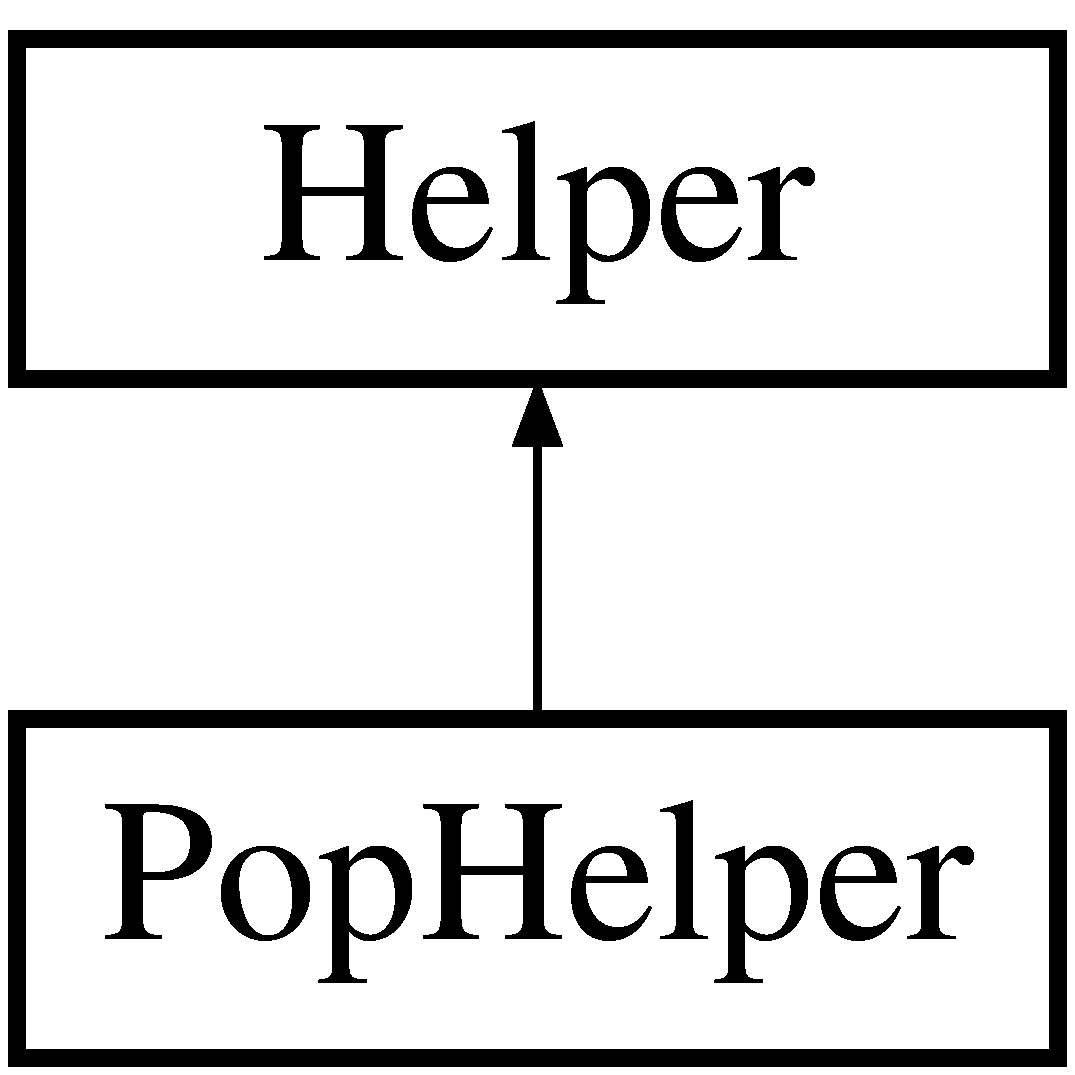
\includegraphics[height=2.000000cm]{class_pop_helper}
\end{center}
\end{figure}
\subsection*{Public Member Functions}
\begin{DoxyCompactItemize}
\item 
void \hyperlink{class_pop_helper_afc46783535b23c91f252e182d771ae3f}{init} (\hyperlink{class_pop_op}{Pop\+Op} $\ast$cop)
\item 
\hyperlink{class_pop_helper_a3d5d4f3c3cf005787a9cefabbfe895ed}{Pop\+Helper} ()
\item 
\hyperlink{class_pop_helper_a4258b16f767e4dff8e9799032903d4ce}{Pop\+Helper} (\hyperlink{class_pop_op}{Pop\+Op} $\ast$cop)
\item 
bool \hyperlink{class_pop_helper_a74d0a4ce1e4f8d2705fc69a014bfc924}{complete} (W\+F\+Vector $\ast$vec, int pos)
\item 
bool \hyperlink{class_pop_helper_a9902a2778674e0577b9c84f3c7a52a0d}{get\+Result} (void $\ast$\&v)
\item 
bool \hyperlink{class_pop_helper_a53b61d8fd4386a4cec5fca6ef399d284}{try\+Free} ()
\item 
bool \hyperlink{class_pop_helper_a9fd70c008d5bded56884fd78030f4d56}{watch} (void $\ast$p, Array\+Element $\ast$a)
\item 
void \hyperlink{class_pop_helper_a15c8fd43c7291a6750f7e66c737f2593}{unwatch} ()
\item 
bool \hyperlink{class_pop_helper_a2c831cbed796924dfdad5e5bd1bdd4c3}{is\+Watched} ()
\item 
void $\ast$ \hyperlink{class_pop_helper_a83b4ba96b55bf0f32e288e73b0af2d32}{read\+Through} ()
\end{DoxyCompactItemize}
\subsection*{Public Attributes}
\begin{DoxyCompactItemize}
\item 
std\+::atomic$<$ void $\ast$ $>$ \hyperlink{class_pop_helper_a4dec73ec5d4d34f54634b18c325262b3}{child}
\item 
\hyperlink{class_pop_op}{Pop\+Op} $\ast$ \hyperlink{class_pop_helper_a8997d99ba6a2a7449d2fcf4ed6e99340}{control\+Op}
\end{DoxyCompactItemize}


\subsection{Constructor \& Destructor Documentation}
\hypertarget{class_pop_helper_a3d5d4f3c3cf005787a9cefabbfe895ed}{}\index{Pop\+Helper@{Pop\+Helper}!Pop\+Helper@{Pop\+Helper}}
\index{Pop\+Helper@{Pop\+Helper}!Pop\+Helper@{Pop\+Helper}}
\subsubsection[{Pop\+Helper()}]{\setlength{\rightskip}{0pt plus 5cm}Pop\+Helper\+::\+Pop\+Helper (
\begin{DoxyParamCaption}
{}
\end{DoxyParamCaption}
)\hspace{0.3cm}{\ttfamily [inline]}}\label{class_pop_helper_a3d5d4f3c3cf005787a9cefabbfe895ed}
\hypertarget{class_pop_helper_a4258b16f767e4dff8e9799032903d4ce}{}\index{Pop\+Helper@{Pop\+Helper}!Pop\+Helper@{Pop\+Helper}}
\index{Pop\+Helper@{Pop\+Helper}!Pop\+Helper@{Pop\+Helper}}
\subsubsection[{Pop\+Helper(\+Pop\+Op $\ast$cop)}]{\setlength{\rightskip}{0pt plus 5cm}Pop\+Helper\+::\+Pop\+Helper (
\begin{DoxyParamCaption}
\item[{{\bf Pop\+Op} $\ast$}]{cop}
\end{DoxyParamCaption}
)\hspace{0.3cm}{\ttfamily [inline]}}\label{class_pop_helper_a4258b16f767e4dff8e9799032903d4ce}


\subsection{Member Function Documentation}
\hypertarget{class_pop_helper_a74d0a4ce1e4f8d2705fc69a014bfc924}{}\index{Pop\+Helper@{Pop\+Helper}!complete@{complete}}
\index{complete@{complete}!Pop\+Helper@{Pop\+Helper}}
\subsubsection[{complete(\+W\+F\+Vector $\ast$vec, int pos)}]{\setlength{\rightskip}{0pt plus 5cm}bool Pop\+Helper\+::complete (
\begin{DoxyParamCaption}
\item[{W\+F\+Vector $\ast$}]{vec, }
\item[{int}]{pos}
\end{DoxyParamCaption}
)}\label{class_pop_helper_a74d0a4ce1e4f8d2705fc69a014bfc924}
\hypertarget{class_pop_helper_a9902a2778674e0577b9c84f3c7a52a0d}{}\index{Pop\+Helper@{Pop\+Helper}!get\+Result@{get\+Result}}
\index{get\+Result@{get\+Result}!Pop\+Helper@{Pop\+Helper}}
\subsubsection[{get\+Result(void $\ast$\&v)}]{\setlength{\rightskip}{0pt plus 5cm}bool Pop\+Helper\+::get\+Result (
\begin{DoxyParamCaption}
\item[{void $\ast$\&}]{v}
\end{DoxyParamCaption}
)}\label{class_pop_helper_a9902a2778674e0577b9c84f3c7a52a0d}
\hypertarget{class_pop_helper_afc46783535b23c91f252e182d771ae3f}{}\index{Pop\+Helper@{Pop\+Helper}!init@{init}}
\index{init@{init}!Pop\+Helper@{Pop\+Helper}}
\subsubsection[{init(\+Pop\+Op $\ast$cop)}]{\setlength{\rightskip}{0pt plus 5cm}void Pop\+Helper\+::init (
\begin{DoxyParamCaption}
\item[{{\bf Pop\+Op} $\ast$}]{cop}
\end{DoxyParamCaption}
)\hspace{0.3cm}{\ttfamily [inline]}}\label{class_pop_helper_afc46783535b23c91f252e182d771ae3f}
\hypertarget{class_pop_helper_a2c831cbed796924dfdad5e5bd1bdd4c3}{}\index{Pop\+Helper@{Pop\+Helper}!is\+Watched@{is\+Watched}}
\index{is\+Watched@{is\+Watched}!Pop\+Helper@{Pop\+Helper}}
\subsubsection[{is\+Watched()}]{\setlength{\rightskip}{0pt plus 5cm}bool Pop\+Helper\+::is\+Watched (
\begin{DoxyParamCaption}
{}
\end{DoxyParamCaption}
)\hspace{0.3cm}{\ttfamily [inline]}}\label{class_pop_helper_a2c831cbed796924dfdad5e5bd1bdd4c3}
\hypertarget{class_pop_helper_a83b4ba96b55bf0f32e288e73b0af2d32}{}\index{Pop\+Helper@{Pop\+Helper}!read\+Through@{read\+Through}}
\index{read\+Through@{read\+Through}!Pop\+Helper@{Pop\+Helper}}
\subsubsection[{read\+Through()}]{\setlength{\rightskip}{0pt plus 5cm}void$\ast$ Pop\+Helper\+::read\+Through (
\begin{DoxyParamCaption}
{}
\end{DoxyParamCaption}
)\hspace{0.3cm}{\ttfamily [inline]}}\label{class_pop_helper_a83b4ba96b55bf0f32e288e73b0af2d32}
\hypertarget{class_pop_helper_a53b61d8fd4386a4cec5fca6ef399d284}{}\index{Pop\+Helper@{Pop\+Helper}!try\+Free@{try\+Free}}
\index{try\+Free@{try\+Free}!Pop\+Helper@{Pop\+Helper}}
\subsubsection[{try\+Free()}]{\setlength{\rightskip}{0pt plus 5cm}bool Pop\+Helper\+::try\+Free (
\begin{DoxyParamCaption}
{}
\end{DoxyParamCaption}
)}\label{class_pop_helper_a53b61d8fd4386a4cec5fca6ef399d284}
\hypertarget{class_pop_helper_a15c8fd43c7291a6750f7e66c737f2593}{}\index{Pop\+Helper@{Pop\+Helper}!unwatch@{unwatch}}
\index{unwatch@{unwatch}!Pop\+Helper@{Pop\+Helper}}
\subsubsection[{unwatch()}]{\setlength{\rightskip}{0pt plus 5cm}void Pop\+Helper\+::unwatch (
\begin{DoxyParamCaption}
{}
\end{DoxyParamCaption}
)\hspace{0.3cm}{\ttfamily [inline]}}\label{class_pop_helper_a15c8fd43c7291a6750f7e66c737f2593}
\hypertarget{class_pop_helper_a9fd70c008d5bded56884fd78030f4d56}{}\index{Pop\+Helper@{Pop\+Helper}!watch@{watch}}
\index{watch@{watch}!Pop\+Helper@{Pop\+Helper}}
\subsubsection[{watch(void $\ast$p, Array\+Element $\ast$a)}]{\setlength{\rightskip}{0pt plus 5cm}bool Pop\+Helper\+::watch (
\begin{DoxyParamCaption}
\item[{void $\ast$}]{p, }
\item[{Array\+Element $\ast$}]{a}
\end{DoxyParamCaption}
)\hspace{0.3cm}{\ttfamily [inline]}}\label{class_pop_helper_a9fd70c008d5bded56884fd78030f4d56}


\subsection{Member Data Documentation}
\hypertarget{class_pop_helper_a4dec73ec5d4d34f54634b18c325262b3}{}\index{Pop\+Helper@{Pop\+Helper}!child@{child}}
\index{child@{child}!Pop\+Helper@{Pop\+Helper}}
\subsubsection[{child}]{\setlength{\rightskip}{0pt plus 5cm}std\+::atomic$<$void $\ast$$>$ Pop\+Helper\+::child}\label{class_pop_helper_a4dec73ec5d4d34f54634b18c325262b3}
\hypertarget{class_pop_helper_a8997d99ba6a2a7449d2fcf4ed6e99340}{}\index{Pop\+Helper@{Pop\+Helper}!control\+Op@{control\+Op}}
\index{control\+Op@{control\+Op}!Pop\+Helper@{Pop\+Helper}}
\subsubsection[{control\+Op}]{\setlength{\rightskip}{0pt plus 5cm}{\bf Pop\+Op}$\ast$ Pop\+Helper\+::control\+Op}\label{class_pop_helper_a8997d99ba6a2a7449d2fcf4ed6e99340}


The documentation for this class was generated from the following file\+:\begin{DoxyCompactItemize}
\item 
tervel/containers/wf/vector/old/\hyperlink{pop__helper_8h}{pop\+\_\+helper.\+h}\end{DoxyCompactItemize}

\hypertarget{class_pop_op}{}\section{Pop\+Op Class Reference}
\label{class_pop_op}\index{Pop\+Op@{Pop\+Op}}


{\ttfamily \#include $<$pop\+\_\+op.\+h$>$}

Inheritance diagram for Pop\+Op\+:\begin{figure}[H]
\begin{center}
\leavevmode
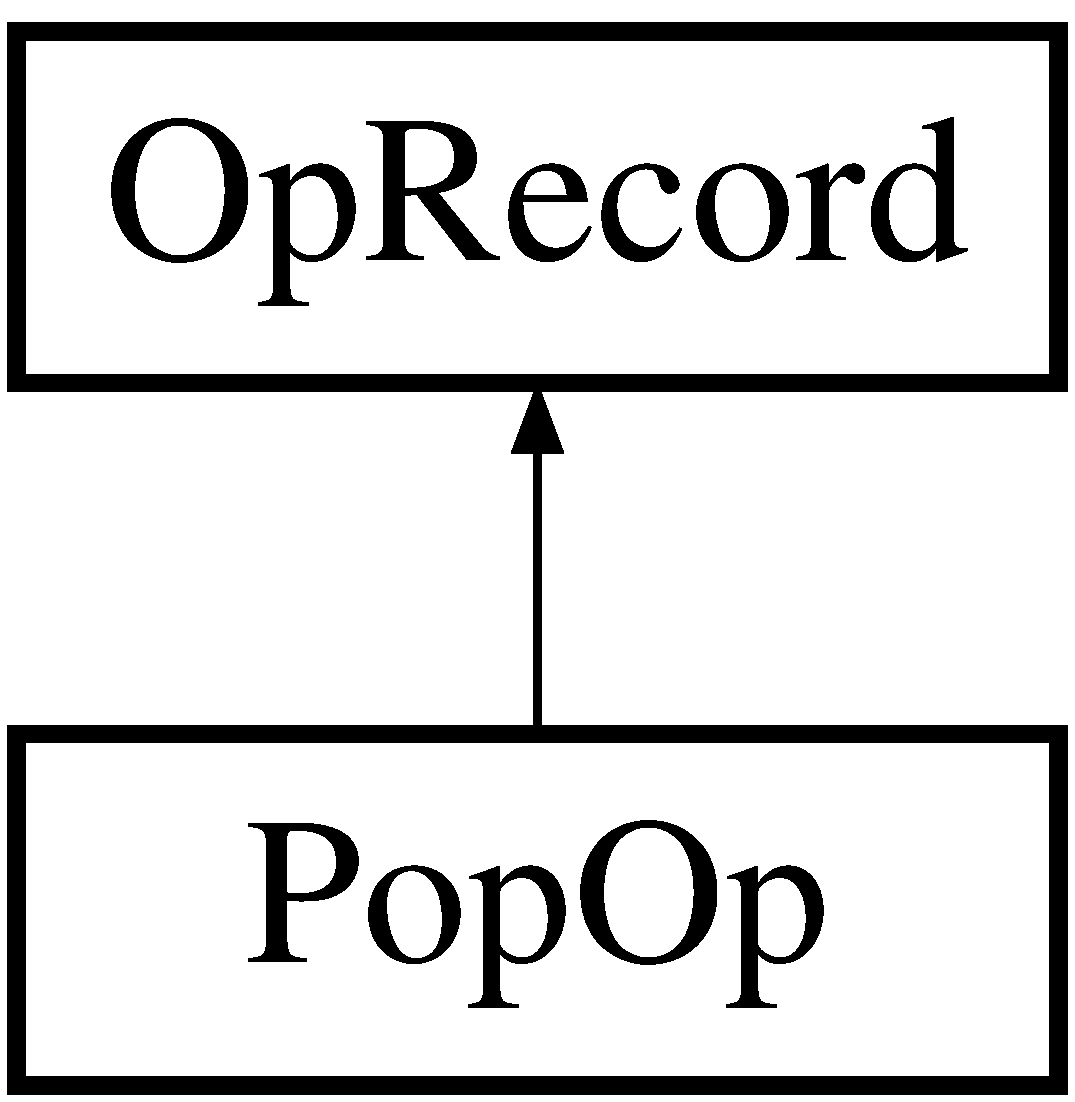
\includegraphics[height=2.000000cm]{class_pop_op}
\end{center}
\end{figure}
\subsection*{Public Member Functions}
\begin{DoxyCompactItemize}
\item 
\hyperlink{class_pop_op_a892b7f55547a7bd14ed03e16da429c4b}{Pop\+Op} ()
\item 
void $\ast$ \hyperlink{class_pop_op_afdea3c00a83ab27ca50a5283ad6f7834}{begin} (W\+F\+Vector $\ast$vec)
\item 
void $\ast$ \hyperlink{class_pop_op_a4fbff3f17df43cc3d3000fe5bdb02ed6}{s\+\_\+execute} (W\+F\+Vector $\ast$vec)
\item 
void \hyperlink{class_pop_op_a5916f1f444527aa67a32e8a38935e21c}{execute} (W\+F\+Vector $\ast$vec)
\item 
bool \hyperlink{class_pop_op_af6ae772dbf74cda9c10ced07939a4e21}{try\+Free} ()
\end{DoxyCompactItemize}
\subsection*{Public Attributes}
\begin{DoxyCompactItemize}
\item 
std\+::atomic$<$ \hyperlink{class_pop_helper}{Pop\+Helper} $\ast$ $>$ \hyperlink{class_pop_op_a54a10dfdaa44c82037f5a50a03aab0a5}{assoc}
\end{DoxyCompactItemize}


\subsection{Constructor \& Destructor Documentation}
\hypertarget{class_pop_op_a892b7f55547a7bd14ed03e16da429c4b}{}\index{Pop\+Op@{Pop\+Op}!Pop\+Op@{Pop\+Op}}
\index{Pop\+Op@{Pop\+Op}!Pop\+Op@{Pop\+Op}}
\subsubsection[{Pop\+Op()}]{\setlength{\rightskip}{0pt plus 5cm}Pop\+Op\+::\+Pop\+Op (
\begin{DoxyParamCaption}
{}
\end{DoxyParamCaption}
)\hspace{0.3cm}{\ttfamily [inline]}}\label{class_pop_op_a892b7f55547a7bd14ed03e16da429c4b}


\subsection{Member Function Documentation}
\hypertarget{class_pop_op_afdea3c00a83ab27ca50a5283ad6f7834}{}\index{Pop\+Op@{Pop\+Op}!begin@{begin}}
\index{begin@{begin}!Pop\+Op@{Pop\+Op}}
\subsubsection[{begin(\+W\+F\+Vector $\ast$vec)}]{\setlength{\rightskip}{0pt plus 5cm}void $\ast$ Pop\+Op\+::begin (
\begin{DoxyParamCaption}
\item[{W\+F\+Vector $\ast$}]{vec}
\end{DoxyParamCaption}
)}\label{class_pop_op_afdea3c00a83ab27ca50a5283ad6f7834}
\hypertarget{class_pop_op_a5916f1f444527aa67a32e8a38935e21c}{}\index{Pop\+Op@{Pop\+Op}!execute@{execute}}
\index{execute@{execute}!Pop\+Op@{Pop\+Op}}
\subsubsection[{execute(\+W\+F\+Vector $\ast$vec)}]{\setlength{\rightskip}{0pt plus 5cm}void Pop\+Op\+::execute (
\begin{DoxyParamCaption}
\item[{W\+F\+Vector $\ast$}]{vec}
\end{DoxyParamCaption}
)\hspace{0.3cm}{\ttfamily [inline]}}\label{class_pop_op_a5916f1f444527aa67a32e8a38935e21c}
\hypertarget{class_pop_op_a4fbff3f17df43cc3d3000fe5bdb02ed6}{}\index{Pop\+Op@{Pop\+Op}!s\+\_\+execute@{s\+\_\+execute}}
\index{s\+\_\+execute@{s\+\_\+execute}!Pop\+Op@{Pop\+Op}}
\subsubsection[{s\+\_\+execute(\+W\+F\+Vector $\ast$vec)}]{\setlength{\rightskip}{0pt plus 5cm}void $\ast$ Pop\+Op\+::s\+\_\+execute (
\begin{DoxyParamCaption}
\item[{W\+F\+Vector $\ast$}]{vec}
\end{DoxyParamCaption}
)}\label{class_pop_op_a4fbff3f17df43cc3d3000fe5bdb02ed6}
\hypertarget{class_pop_op_af6ae772dbf74cda9c10ced07939a4e21}{}\index{Pop\+Op@{Pop\+Op}!try\+Free@{try\+Free}}
\index{try\+Free@{try\+Free}!Pop\+Op@{Pop\+Op}}
\subsubsection[{try\+Free()}]{\setlength{\rightskip}{0pt plus 5cm}bool Pop\+Op\+::try\+Free (
\begin{DoxyParamCaption}
{}
\end{DoxyParamCaption}
)}\label{class_pop_op_af6ae772dbf74cda9c10ced07939a4e21}


\subsection{Member Data Documentation}
\hypertarget{class_pop_op_a54a10dfdaa44c82037f5a50a03aab0a5}{}\index{Pop\+Op@{Pop\+Op}!assoc@{assoc}}
\index{assoc@{assoc}!Pop\+Op@{Pop\+Op}}
\subsubsection[{assoc}]{\setlength{\rightskip}{0pt plus 5cm}std\+::atomic$<${\bf Pop\+Helper} $\ast$$>$ Pop\+Op\+::assoc}\label{class_pop_op_a54a10dfdaa44c82037f5a50a03aab0a5}


The documentation for this class was generated from the following files\+:\begin{DoxyCompactItemize}
\item 
tervel/containers/wf/vector/old/\hyperlink{pop__op_8h}{pop\+\_\+op.\+h}\item 
tervel/containers/wf/vector/old/\hyperlink{pop__helper_8h}{pop\+\_\+helper.\+h}\end{DoxyCompactItemize}

\hypertarget{classtervel_1_1containers_1_1wf_1_1vector_1_1_pop_op}{}\section{tervel\+:\+:containers\+:\+:wf\+:\+:vector\+:\+:Pop\+Op$<$ T $>$ Class Template Reference}
\label{classtervel_1_1containers_1_1wf_1_1vector_1_1_pop_op}\index{tervel\+::containers\+::wf\+::vector\+::\+Pop\+Op$<$ T $>$@{tervel\+::containers\+::wf\+::vector\+::\+Pop\+Op$<$ T $>$}}


{\ttfamily \#include $<$popback\+\_\+op.\+h$>$}

Inheritance diagram for tervel\+:\+:containers\+:\+:wf\+:\+:vector\+:\+:Pop\+Op$<$ T $>$\+:\begin{figure}[H]
\begin{center}
\leavevmode
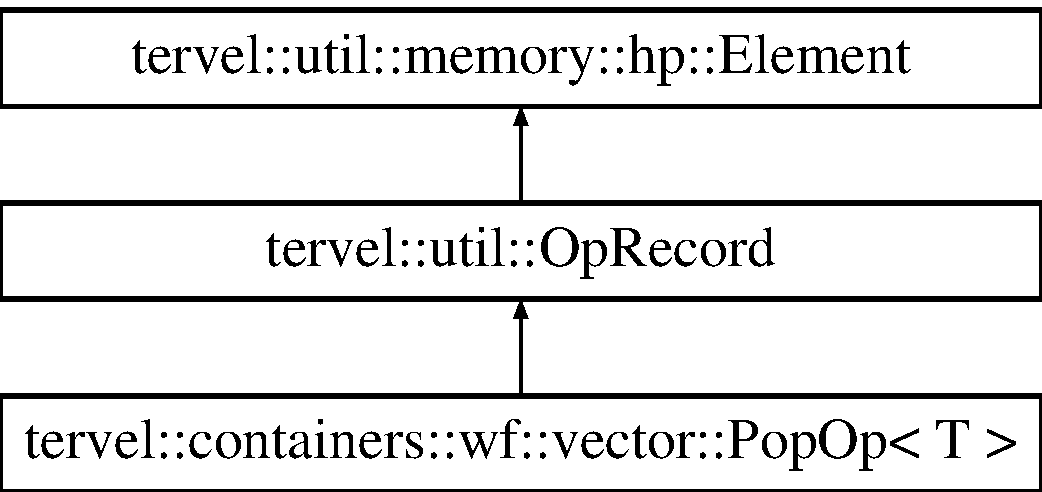
\includegraphics[height=3.000000cm]{classtervel_1_1containers_1_1wf_1_1vector_1_1_pop_op}
\end{center}
\end{figure}
\subsection*{Public Member Functions}
\begin{DoxyCompactItemize}
\item 
\hyperlink{classtervel_1_1containers_1_1wf_1_1vector_1_1_pop_op_acec5a8f43e480109f9e4c7edcdada373}{Pop\+Op} (Vector$<$ T $>$ $\ast$vec)
\item 
\hyperlink{classtervel_1_1containers_1_1wf_1_1vector_1_1_pop_op_afe1ff098c9530cdc332b6c5af646b435}{$\sim$\+Pop\+Op} ()
\item 
bool \hyperlink{classtervel_1_1containers_1_1wf_1_1vector_1_1_pop_op_a71d9e27ccf6ec78d6001e630b9357e5b}{result} (T \&val)
\item 
bool \hyperlink{classtervel_1_1containers_1_1wf_1_1vector_1_1_pop_op_a2312e7a8857bbf35e3c97df89ca72598}{result} ()
\item 
void \hyperlink{classtervel_1_1containers_1_1wf_1_1vector_1_1_pop_op_ac997893b45ab02efe3c2e705bc4a24ae}{set\+\_\+failed} ()
\item 
void \hyperlink{classtervel_1_1containers_1_1wf_1_1vector_1_1_pop_op_abd820a976a7f356f87ed8dadddef12c4}{help\+\_\+complete} ()
\begin{DoxyCompactList}\small\item\em Implementations of this function that upon its return the operation described in the Op\+Record has been completed. \end{DoxyCompactList}\item 
bool \hyperlink{classtervel_1_1containers_1_1wf_1_1vector_1_1_pop_op_a33e196246b45105b1a7be0f7f3e4cd35}{is\+\_\+watched} ()
\end{DoxyCompactItemize}
\subsection*{Static Public Member Functions}
\begin{DoxyCompactItemize}
\item 
static bool \hyperlink{classtervel_1_1containers_1_1wf_1_1vector_1_1_pop_op_a54386e257528936796ac13e7ca72394a}{execute} (Vector$<$ T $>$ $\ast$vec, T \&val)
\end{DoxyCompactItemize}
\subsection*{Static Public Attributes}
\begin{DoxyCompactItemize}
\item 
static constexpr \hyperlink{classtervel_1_1containers_1_1wf_1_1vector_1_1_pop_op_helper}{Pop\+Op\+Helper}$<$ T $>$ $\ast$ \hyperlink{classtervel_1_1containers_1_1wf_1_1vector_1_1_pop_op_a2f0d5f83e90cec090ec83ae5ba5d056b}{is\+\_\+empty\+\_\+const} \{reinterpret\+\_\+cast$<$\hyperlink{classtervel_1_1containers_1_1wf_1_1vector_1_1_pop_op_helper}{Pop\+Op\+Helper}$<$T$>$ $\ast$$>$(0x1\+L)\}
\end{DoxyCompactItemize}
\subsection*{Private Attributes}
\begin{DoxyCompactItemize}
\item 
Vector$<$ T $>$ $\ast$ \hyperlink{classtervel_1_1containers_1_1wf_1_1vector_1_1_pop_op_a32b0803cfcf70ab2b86b59b6790eb676}{vec\+\_\+}
\item 
std\+::atomic$<$ T $>$ $\ast$ \hyperlink{classtervel_1_1containers_1_1wf_1_1vector_1_1_pop_op_afedc8c1eafbacd0601a72c43fd1dc521}{prev\+\_\+spot\+\_\+} \{nullptr\}
\item 
std\+::atomic$<$ \hyperlink{classtervel_1_1containers_1_1wf_1_1vector_1_1_pop_op_helper}{Pop\+Op\+Helper}$<$ T $>$ $\ast$ $>$ \hyperlink{classtervel_1_1containers_1_1wf_1_1vector_1_1_pop_op_a628660acd654de451aa0554f365a458d}{helper\+\_\+} \{nullptr\}
\end{DoxyCompactItemize}
\subsection*{Friends}
\begin{DoxyCompactItemize}
\item 
class \hyperlink{classtervel_1_1containers_1_1wf_1_1vector_1_1_pop_op_a3c1a5b124243e3f3d5eb89eb57751655}{Pop\+Op\+Helper$<$ T $>$}
\end{DoxyCompactItemize}


\subsection{Constructor \& Destructor Documentation}
\hypertarget{classtervel_1_1containers_1_1wf_1_1vector_1_1_pop_op_acec5a8f43e480109f9e4c7edcdada373}{}\index{tervel\+::containers\+::wf\+::vector\+::\+Pop\+Op@{tervel\+::containers\+::wf\+::vector\+::\+Pop\+Op}!Pop\+Op@{Pop\+Op}}
\index{Pop\+Op@{Pop\+Op}!tervel\+::containers\+::wf\+::vector\+::\+Pop\+Op@{tervel\+::containers\+::wf\+::vector\+::\+Pop\+Op}}
\subsubsection[{Pop\+Op(\+Vector$<$ T $>$ $\ast$vec)}]{\setlength{\rightskip}{0pt plus 5cm}template$<$typename T$>$ {\bf tervel\+::containers\+::wf\+::vector\+::\+Pop\+Op}$<$ T $>$\+::{\bf Pop\+Op} (
\begin{DoxyParamCaption}
\item[{Vector$<$ T $>$ $\ast$}]{vec}
\end{DoxyParamCaption}
)\hspace{0.3cm}{\ttfamily [inline]}}\label{classtervel_1_1containers_1_1wf_1_1vector_1_1_pop_op_acec5a8f43e480109f9e4c7edcdada373}
\hypertarget{classtervel_1_1containers_1_1wf_1_1vector_1_1_pop_op_afe1ff098c9530cdc332b6c5af646b435}{}\index{tervel\+::containers\+::wf\+::vector\+::\+Pop\+Op@{tervel\+::containers\+::wf\+::vector\+::\+Pop\+Op}!````~Pop\+Op@{$\sim$\+Pop\+Op}}
\index{````~Pop\+Op@{$\sim$\+Pop\+Op}!tervel\+::containers\+::wf\+::vector\+::\+Pop\+Op@{tervel\+::containers\+::wf\+::vector\+::\+Pop\+Op}}
\subsubsection[{$\sim$\+Pop\+Op()}]{\setlength{\rightskip}{0pt plus 5cm}template$<$typename T$>$ {\bf tervel\+::containers\+::wf\+::vector\+::\+Pop\+Op}$<$ T $>$\+::$\sim${\bf Pop\+Op} (
\begin{DoxyParamCaption}
{}
\end{DoxyParamCaption}
)\hspace{0.3cm}{\ttfamily [inline]}}\label{classtervel_1_1containers_1_1wf_1_1vector_1_1_pop_op_afe1ff098c9530cdc332b6c5af646b435}


\subsection{Member Function Documentation}
\hypertarget{classtervel_1_1containers_1_1wf_1_1vector_1_1_pop_op_a54386e257528936796ac13e7ca72394a}{}\index{tervel\+::containers\+::wf\+::vector\+::\+Pop\+Op@{tervel\+::containers\+::wf\+::vector\+::\+Pop\+Op}!execute@{execute}}
\index{execute@{execute}!tervel\+::containers\+::wf\+::vector\+::\+Pop\+Op@{tervel\+::containers\+::wf\+::vector\+::\+Pop\+Op}}
\subsubsection[{execute(\+Vector$<$ T $>$ $\ast$vec, T \&val)}]{\setlength{\rightskip}{0pt plus 5cm}template$<$typename T$>$ static bool {\bf tervel\+::containers\+::wf\+::vector\+::\+Pop\+Op}$<$ T $>$\+::execute (
\begin{DoxyParamCaption}
\item[{Vector$<$ T $>$ $\ast$}]{vec, }
\item[{T \&}]{val}
\end{DoxyParamCaption}
)\hspace{0.3cm}{\ttfamily [inline]}, {\ttfamily [static]}}\label{classtervel_1_1containers_1_1wf_1_1vector_1_1_pop_op_a54386e257528936796ac13e7ca72394a}
\hypertarget{classtervel_1_1containers_1_1wf_1_1vector_1_1_pop_op_abd820a976a7f356f87ed8dadddef12c4}{}\index{tervel\+::containers\+::wf\+::vector\+::\+Pop\+Op@{tervel\+::containers\+::wf\+::vector\+::\+Pop\+Op}!help\+\_\+complete@{help\+\_\+complete}}
\index{help\+\_\+complete@{help\+\_\+complete}!tervel\+::containers\+::wf\+::vector\+::\+Pop\+Op@{tervel\+::containers\+::wf\+::vector\+::\+Pop\+Op}}
\subsubsection[{help\+\_\+complete()}]{\setlength{\rightskip}{0pt plus 5cm}template$<$typename T$>$ void {\bf tervel\+::containers\+::wf\+::vector\+::\+Pop\+Op}$<$ T $>$\+::help\+\_\+complete (
\begin{DoxyParamCaption}
{}
\end{DoxyParamCaption}
)\hspace{0.3cm}{\ttfamily [inline]}, {\ttfamily [virtual]}}\label{classtervel_1_1containers_1_1wf_1_1vector_1_1_pop_op_abd820a976a7f356f87ed8dadddef12c4}


Implementations of this function that upon its return the operation described in the Op\+Record has been completed. 

As such it must be thread-\/safe and the extending class must contain all the information necessary to complete the operation. 

Implements \hyperlink{classtervel_1_1util_1_1_op_record_aa75ab39688a8d4cceb6a1ef0409537c0}{tervel\+::util\+::\+Op\+Record}.

\hypertarget{classtervel_1_1containers_1_1wf_1_1vector_1_1_pop_op_a33e196246b45105b1a7be0f7f3e4cd35}{}\index{tervel\+::containers\+::wf\+::vector\+::\+Pop\+Op@{tervel\+::containers\+::wf\+::vector\+::\+Pop\+Op}!is\+\_\+watched@{is\+\_\+watched}}
\index{is\+\_\+watched@{is\+\_\+watched}!tervel\+::containers\+::wf\+::vector\+::\+Pop\+Op@{tervel\+::containers\+::wf\+::vector\+::\+Pop\+Op}}
\subsubsection[{is\+\_\+watched()}]{\setlength{\rightskip}{0pt plus 5cm}template$<$typename T$>$ bool {\bf tervel\+::containers\+::wf\+::vector\+::\+Pop\+Op}$<$ T $>$\+::is\+\_\+watched (
\begin{DoxyParamCaption}
{}
\end{DoxyParamCaption}
)\hspace{0.3cm}{\ttfamily [inline]}}\label{classtervel_1_1containers_1_1wf_1_1vector_1_1_pop_op_a33e196246b45105b1a7be0f7f3e4cd35}
\hypertarget{classtervel_1_1containers_1_1wf_1_1vector_1_1_pop_op_a71d9e27ccf6ec78d6001e630b9357e5b}{}\index{tervel\+::containers\+::wf\+::vector\+::\+Pop\+Op@{tervel\+::containers\+::wf\+::vector\+::\+Pop\+Op}!result@{result}}
\index{result@{result}!tervel\+::containers\+::wf\+::vector\+::\+Pop\+Op@{tervel\+::containers\+::wf\+::vector\+::\+Pop\+Op}}
\subsubsection[{result(\+T \&val)}]{\setlength{\rightskip}{0pt plus 5cm}template$<$typename T$>$ bool {\bf tervel\+::containers\+::wf\+::vector\+::\+Pop\+Op}$<$ T $>$\+::result (
\begin{DoxyParamCaption}
\item[{T \&}]{val}
\end{DoxyParamCaption}
)\hspace{0.3cm}{\ttfamily [inline]}}\label{classtervel_1_1containers_1_1wf_1_1vector_1_1_pop_op_a71d9e27ccf6ec78d6001e630b9357e5b}
\hypertarget{classtervel_1_1containers_1_1wf_1_1vector_1_1_pop_op_a2312e7a8857bbf35e3c97df89ca72598}{}\index{tervel\+::containers\+::wf\+::vector\+::\+Pop\+Op@{tervel\+::containers\+::wf\+::vector\+::\+Pop\+Op}!result@{result}}
\index{result@{result}!tervel\+::containers\+::wf\+::vector\+::\+Pop\+Op@{tervel\+::containers\+::wf\+::vector\+::\+Pop\+Op}}
\subsubsection[{result()}]{\setlength{\rightskip}{0pt plus 5cm}template$<$typename T$>$ bool {\bf tervel\+::containers\+::wf\+::vector\+::\+Pop\+Op}$<$ T $>$\+::result (
\begin{DoxyParamCaption}
{}
\end{DoxyParamCaption}
)\hspace{0.3cm}{\ttfamily [inline]}}\label{classtervel_1_1containers_1_1wf_1_1vector_1_1_pop_op_a2312e7a8857bbf35e3c97df89ca72598}
\hypertarget{classtervel_1_1containers_1_1wf_1_1vector_1_1_pop_op_ac997893b45ab02efe3c2e705bc4a24ae}{}\index{tervel\+::containers\+::wf\+::vector\+::\+Pop\+Op@{tervel\+::containers\+::wf\+::vector\+::\+Pop\+Op}!set\+\_\+failed@{set\+\_\+failed}}
\index{set\+\_\+failed@{set\+\_\+failed}!tervel\+::containers\+::wf\+::vector\+::\+Pop\+Op@{tervel\+::containers\+::wf\+::vector\+::\+Pop\+Op}}
\subsubsection[{set\+\_\+failed()}]{\setlength{\rightskip}{0pt plus 5cm}template$<$typename T$>$ void {\bf tervel\+::containers\+::wf\+::vector\+::\+Pop\+Op}$<$ T $>$\+::set\+\_\+failed (
\begin{DoxyParamCaption}
{}
\end{DoxyParamCaption}
)\hspace{0.3cm}{\ttfamily [inline]}}\label{classtervel_1_1containers_1_1wf_1_1vector_1_1_pop_op_ac997893b45ab02efe3c2e705bc4a24ae}


\subsection{Friends And Related Function Documentation}
\hypertarget{classtervel_1_1containers_1_1wf_1_1vector_1_1_pop_op_a3c1a5b124243e3f3d5eb89eb57751655}{}\index{tervel\+::containers\+::wf\+::vector\+::\+Pop\+Op@{tervel\+::containers\+::wf\+::vector\+::\+Pop\+Op}!Pop\+Op\+Helper$<$ T $>$@{Pop\+Op\+Helper$<$ T $>$}}
\index{Pop\+Op\+Helper$<$ T $>$@{Pop\+Op\+Helper$<$ T $>$}!tervel\+::containers\+::wf\+::vector\+::\+Pop\+Op@{tervel\+::containers\+::wf\+::vector\+::\+Pop\+Op}}
\subsubsection[{Pop\+Op\+Helper$<$ T $>$}]{\setlength{\rightskip}{0pt plus 5cm}template$<$typename T$>$ friend class {\bf Pop\+Op\+Helper}$<$ T $>$\hspace{0.3cm}{\ttfamily [friend]}}\label{classtervel_1_1containers_1_1wf_1_1vector_1_1_pop_op_a3c1a5b124243e3f3d5eb89eb57751655}


\subsection{Member Data Documentation}
\hypertarget{classtervel_1_1containers_1_1wf_1_1vector_1_1_pop_op_a628660acd654de451aa0554f365a458d}{}\index{tervel\+::containers\+::wf\+::vector\+::\+Pop\+Op@{tervel\+::containers\+::wf\+::vector\+::\+Pop\+Op}!helper\+\_\+@{helper\+\_\+}}
\index{helper\+\_\+@{helper\+\_\+}!tervel\+::containers\+::wf\+::vector\+::\+Pop\+Op@{tervel\+::containers\+::wf\+::vector\+::\+Pop\+Op}}
\subsubsection[{helper\+\_\+}]{\setlength{\rightskip}{0pt plus 5cm}template$<$typename T$>$ std\+::atomic$<${\bf Pop\+Op\+Helper}$<$T$>$ $\ast$$>$ {\bf tervel\+::containers\+::wf\+::vector\+::\+Pop\+Op}$<$ T $>$\+::helper\+\_\+ \{nullptr\}\hspace{0.3cm}{\ttfamily [private]}}\label{classtervel_1_1containers_1_1wf_1_1vector_1_1_pop_op_a628660acd654de451aa0554f365a458d}
\hypertarget{classtervel_1_1containers_1_1wf_1_1vector_1_1_pop_op_a2f0d5f83e90cec090ec83ae5ba5d056b}{}\index{tervel\+::containers\+::wf\+::vector\+::\+Pop\+Op@{tervel\+::containers\+::wf\+::vector\+::\+Pop\+Op}!is\+\_\+empty\+\_\+const@{is\+\_\+empty\+\_\+const}}
\index{is\+\_\+empty\+\_\+const@{is\+\_\+empty\+\_\+const}!tervel\+::containers\+::wf\+::vector\+::\+Pop\+Op@{tervel\+::containers\+::wf\+::vector\+::\+Pop\+Op}}
\subsubsection[{is\+\_\+empty\+\_\+const}]{\setlength{\rightskip}{0pt plus 5cm}template$<$typename T$>$ constexpr {\bf Pop\+Op\+Helper}$<$T$>$$\ast$ {\bf tervel\+::containers\+::wf\+::vector\+::\+Pop\+Op}$<$ T $>$\+::is\+\_\+empty\+\_\+const \{reinterpret\+\_\+cast$<${\bf Pop\+Op\+Helper}$<$T$>$ $\ast$$>$(0x1\+L)\}\hspace{0.3cm}{\ttfamily [static]}}\label{classtervel_1_1containers_1_1wf_1_1vector_1_1_pop_op_a2f0d5f83e90cec090ec83ae5ba5d056b}
\hypertarget{classtervel_1_1containers_1_1wf_1_1vector_1_1_pop_op_afedc8c1eafbacd0601a72c43fd1dc521}{}\index{tervel\+::containers\+::wf\+::vector\+::\+Pop\+Op@{tervel\+::containers\+::wf\+::vector\+::\+Pop\+Op}!prev\+\_\+spot\+\_\+@{prev\+\_\+spot\+\_\+}}
\index{prev\+\_\+spot\+\_\+@{prev\+\_\+spot\+\_\+}!tervel\+::containers\+::wf\+::vector\+::\+Pop\+Op@{tervel\+::containers\+::wf\+::vector\+::\+Pop\+Op}}
\subsubsection[{prev\+\_\+spot\+\_\+}]{\setlength{\rightskip}{0pt plus 5cm}template$<$typename T$>$ std\+::atomic$<$T$>$$\ast$ {\bf tervel\+::containers\+::wf\+::vector\+::\+Pop\+Op}$<$ T $>$\+::prev\+\_\+spot\+\_\+ \{nullptr\}\hspace{0.3cm}{\ttfamily [private]}}\label{classtervel_1_1containers_1_1wf_1_1vector_1_1_pop_op_afedc8c1eafbacd0601a72c43fd1dc521}
\hypertarget{classtervel_1_1containers_1_1wf_1_1vector_1_1_pop_op_a32b0803cfcf70ab2b86b59b6790eb676}{}\index{tervel\+::containers\+::wf\+::vector\+::\+Pop\+Op@{tervel\+::containers\+::wf\+::vector\+::\+Pop\+Op}!vec\+\_\+@{vec\+\_\+}}
\index{vec\+\_\+@{vec\+\_\+}!tervel\+::containers\+::wf\+::vector\+::\+Pop\+Op@{tervel\+::containers\+::wf\+::vector\+::\+Pop\+Op}}
\subsubsection[{vec\+\_\+}]{\setlength{\rightskip}{0pt plus 5cm}template$<$typename T$>$ Vector$<$T$>$$\ast$ {\bf tervel\+::containers\+::wf\+::vector\+::\+Pop\+Op}$<$ T $>$\+::vec\+\_\+\hspace{0.3cm}{\ttfamily [private]}}\label{classtervel_1_1containers_1_1wf_1_1vector_1_1_pop_op_a32b0803cfcf70ab2b86b59b6790eb676}


The documentation for this class was generated from the following file\+:\begin{DoxyCompactItemize}
\item 
tervel/containers/wf/vector/\hyperlink{popback__op_8h}{popback\+\_\+op.\+h}\end{DoxyCompactItemize}

\hypertarget{classtervel_1_1containers_1_1wf_1_1vector_1_1_pop_op_helper}{}\section{tervel\+:\+:containers\+:\+:wf\+:\+:vector\+:\+:Pop\+Op\+Helper$<$ T $>$ Class Template Reference}
\label{classtervel_1_1containers_1_1wf_1_1vector_1_1_pop_op_helper}\index{tervel\+::containers\+::wf\+::vector\+::\+Pop\+Op\+Helper$<$ T $>$@{tervel\+::containers\+::wf\+::vector\+::\+Pop\+Op\+Helper$<$ T $>$}}


{\ttfamily \#include $<$popback\+\_\+op.\+h$>$}

Inheritance diagram for tervel\+:\+:containers\+:\+:wf\+:\+:vector\+:\+:Pop\+Op\+Helper$<$ T $>$\+:\begin{figure}[H]
\begin{center}
\leavevmode
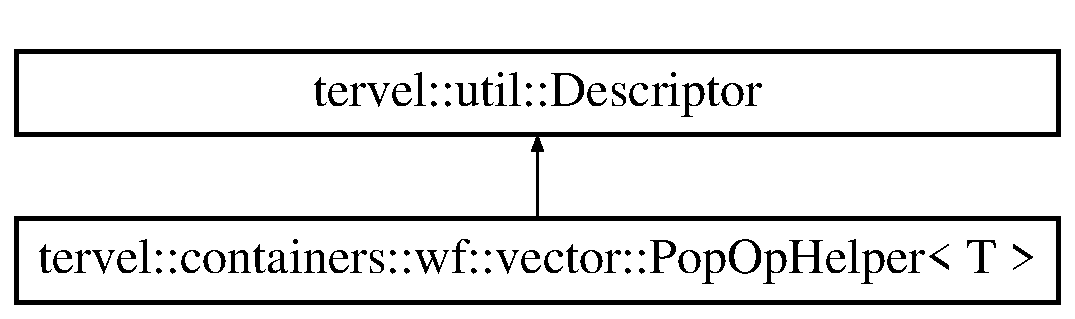
\includegraphics[height=2.000000cm]{classtervel_1_1containers_1_1wf_1_1vector_1_1_pop_op_helper}
\end{center}
\end{figure}
\subsection*{Public Member Functions}
\begin{DoxyCompactItemize}
\item 
\hyperlink{classtervel_1_1containers_1_1wf_1_1vector_1_1_pop_op_helper_a240a07fdf0b2b8dd83118e4561d1d503}{Pop\+Op\+Helper} (Vector$<$ T $>$ $\ast$vec, \hyperlink{classtervel_1_1containers_1_1wf_1_1vector_1_1_pop_op}{Pop\+Op}$<$ T $>$ $\ast$op)
\item 
\hyperlink{classtervel_1_1containers_1_1wf_1_1vector_1_1_pop_op_helper_a5202ccce9347631011450a59c5ccee4b}{Pop\+Op\+Helper} (Vector$<$ T $>$ $\ast$vec)
\item 
\hyperlink{classtervel_1_1containers_1_1wf_1_1vector_1_1_pop_op_helper_a2e3fa09a93946eb888c949c5104320d3}{$\sim$\+Pop\+Op\+Helper} ()
\item 
void \hyperlink{classtervel_1_1containers_1_1wf_1_1vector_1_1_pop_op_helper_a41e3e623caaa4ee222bf3caaf8b550a6}{set\+\_\+prev\+\_\+spot} (std\+::atomic$<$ T $>$ $\ast$prev\+\_\+spot)
\item 
bool \hyperlink{classtervel_1_1containers_1_1wf_1_1vector_1_1_pop_op_helper_ab415614db4dbb5e22d77e22c74fbd3ad}{in\+\_\+progress} ()
\item 
bool \hyperlink{classtervel_1_1containers_1_1wf_1_1vector_1_1_pop_op_helper_a5e9f2e1522a4b12e279d623c164ce77f}{result} (T \&val)
\item 
bool \hyperlink{classtervel_1_1containers_1_1wf_1_1vector_1_1_pop_op_helper_a7d7cee8a5eb40da290c8e3c95f324721}{result} ()
\item 
void \hyperlink{classtervel_1_1containers_1_1wf_1_1vector_1_1_pop_op_helper_ad5e86e41301c8fc8a0254daf285e023f}{fail} ()
\item 
void $\ast$ \hyperlink{classtervel_1_1containers_1_1wf_1_1vector_1_1_pop_op_helper_a0cd831d37361277e4e212e56d453dd70}{get\+\_\+logical\+\_\+value} ()
\begin{DoxyCompactList}\small\item\em This method is implemented by each sub class. \end{DoxyCompactList}\item 
void $\ast$ \hyperlink{classtervel_1_1containers_1_1wf_1_1vector_1_1_pop_op_helper_a1f92037dcfec837afe0684e119c7344f}{complete} (void $\ast$value, std\+::atomic$<$ void $\ast$ $>$ $\ast$address)
\begin{DoxyCompactList}\small\item\em This method is implemented by each sub class and must guarantee that upon return that the descriptor no longer exists at the address it was placed. \end{DoxyCompactList}\item 
bool \hyperlink{classtervel_1_1containers_1_1wf_1_1vector_1_1_pop_op_helper_a7d5839d23d38c1c1762f2b04afb04ff4}{associate} (\hyperlink{classtervel_1_1containers_1_1wf_1_1vector_1_1_pop_op_sub_helper}{Pop\+Op\+Sub\+Helper}$<$ T $>$ $\ast$child)
\item 
bool \hyperlink{classtervel_1_1containers_1_1wf_1_1vector_1_1_pop_op_helper_a2b421b2a3cb984bd94abe3ee254ac819}{on\+\_\+watch} (std\+::atomic$<$ void $\ast$ $>$ $\ast$address, void $\ast$value)
\begin{DoxyCompactList}\small\item\em This method is optional to implement for each sub class. \end{DoxyCompactList}\item 
void \hyperlink{classtervel_1_1containers_1_1wf_1_1vector_1_1_pop_op_helper_a90ee1e07905e336a864184e96d04bf96}{on\+\_\+unwatch} ()
\begin{DoxyCompactList}\small\item\em This method must be implemented if on\+\_\+watch is implemented, and is optional otherwise. \end{DoxyCompactList}\item 
bool \hyperlink{classtervel_1_1containers_1_1wf_1_1vector_1_1_pop_op_helper_afc30533f275eb109ae847e0038404360}{on\+\_\+is\+\_\+watched} ()
\begin{DoxyCompactList}\small\item\em This method is optional to implement for each sub class. \end{DoxyCompactList}\item 
void \hyperlink{classtervel_1_1containers_1_1wf_1_1vector_1_1_pop_op_helper_a54ea71e4dd7949e2b3aa778becf43245}{set\+\_\+control\+\_\+word} ()
\end{DoxyCompactItemize}
\subsection*{Static Public Attributes}
\begin{DoxyCompactItemize}
\item 
static constexpr \hyperlink{classtervel_1_1containers_1_1wf_1_1vector_1_1_pop_op_sub_helper}{Pop\+Op\+Sub\+Helper}$<$ T $>$ $\ast$ \hyperlink{classtervel_1_1containers_1_1wf_1_1vector_1_1_pop_op_helper_a8b5f2f7807984b6a29dbb3b34838eb1f}{fail\+\_\+const} \{reinterpret\+\_\+cast$<$\hyperlink{classtervel_1_1containers_1_1wf_1_1vector_1_1_pop_op_sub_helper}{Pop\+Op\+Sub\+Helper}$<$T$>$ $\ast$$>$(0x1\+L)\}
\end{DoxyCompactItemize}
\subsection*{Private Attributes}
\begin{DoxyCompactItemize}
\item 
Vector$<$ T $>$ $\ast$ \hyperlink{classtervel_1_1containers_1_1wf_1_1vector_1_1_pop_op_helper_a806490bb4410f0becea1ae1dadd27b33}{vec\+\_\+}
\item 
\hyperlink{classtervel_1_1containers_1_1wf_1_1vector_1_1_pop_op}{Pop\+Op}$<$ T $>$ $\ast$ \hyperlink{classtervel_1_1containers_1_1wf_1_1vector_1_1_pop_op_helper_ae44349620db471dd999948a01d590bd8}{op\+\_\+} \{nullptr\}
\item 
std\+::atomic$<$ T $>$ $\ast$ \hyperlink{classtervel_1_1containers_1_1wf_1_1vector_1_1_pop_op_helper_a0a2d49f9ffbee73355ae71e3350d28b7}{prev\+\_\+spot\+\_\+} \{nullptr\}
\item 
std\+::atomic$<$ \hyperlink{classtervel_1_1containers_1_1wf_1_1vector_1_1_pop_op_sub_helper}{Pop\+Op\+Sub\+Helper}$<$ T $>$ $\ast$ $>$ \hyperlink{classtervel_1_1containers_1_1wf_1_1vector_1_1_pop_op_helper_a154a8e3c80060d0a59d3863737180681}{child\+\_\+} \{nullptr\}
\end{DoxyCompactItemize}


\subsection{Constructor \& Destructor Documentation}
\hypertarget{classtervel_1_1containers_1_1wf_1_1vector_1_1_pop_op_helper_a240a07fdf0b2b8dd83118e4561d1d503}{}\index{tervel\+::containers\+::wf\+::vector\+::\+Pop\+Op\+Helper@{tervel\+::containers\+::wf\+::vector\+::\+Pop\+Op\+Helper}!Pop\+Op\+Helper@{Pop\+Op\+Helper}}
\index{Pop\+Op\+Helper@{Pop\+Op\+Helper}!tervel\+::containers\+::wf\+::vector\+::\+Pop\+Op\+Helper@{tervel\+::containers\+::wf\+::vector\+::\+Pop\+Op\+Helper}}
\subsubsection[{Pop\+Op\+Helper(\+Vector$<$ T $>$ $\ast$vec, Pop\+Op$<$ T $>$ $\ast$op)}]{\setlength{\rightskip}{0pt plus 5cm}template$<$typename T$>$ {\bf tervel\+::containers\+::wf\+::vector\+::\+Pop\+Op\+Helper}$<$ T $>$\+::{\bf Pop\+Op\+Helper} (
\begin{DoxyParamCaption}
\item[{Vector$<$ T $>$ $\ast$}]{vec, }
\item[{{\bf Pop\+Op}$<$ T $>$ $\ast$}]{op}
\end{DoxyParamCaption}
)\hspace{0.3cm}{\ttfamily [inline]}}\label{classtervel_1_1containers_1_1wf_1_1vector_1_1_pop_op_helper_a240a07fdf0b2b8dd83118e4561d1d503}
\hypertarget{classtervel_1_1containers_1_1wf_1_1vector_1_1_pop_op_helper_a5202ccce9347631011450a59c5ccee4b}{}\index{tervel\+::containers\+::wf\+::vector\+::\+Pop\+Op\+Helper@{tervel\+::containers\+::wf\+::vector\+::\+Pop\+Op\+Helper}!Pop\+Op\+Helper@{Pop\+Op\+Helper}}
\index{Pop\+Op\+Helper@{Pop\+Op\+Helper}!tervel\+::containers\+::wf\+::vector\+::\+Pop\+Op\+Helper@{tervel\+::containers\+::wf\+::vector\+::\+Pop\+Op\+Helper}}
\subsubsection[{Pop\+Op\+Helper(\+Vector$<$ T $>$ $\ast$vec)}]{\setlength{\rightskip}{0pt plus 5cm}template$<$typename T$>$ {\bf tervel\+::containers\+::wf\+::vector\+::\+Pop\+Op\+Helper}$<$ T $>$\+::{\bf Pop\+Op\+Helper} (
\begin{DoxyParamCaption}
\item[{Vector$<$ T $>$ $\ast$}]{vec}
\end{DoxyParamCaption}
)\hspace{0.3cm}{\ttfamily [inline]}, {\ttfamily [explicit]}}\label{classtervel_1_1containers_1_1wf_1_1vector_1_1_pop_op_helper_a5202ccce9347631011450a59c5ccee4b}
\hypertarget{classtervel_1_1containers_1_1wf_1_1vector_1_1_pop_op_helper_a2e3fa09a93946eb888c949c5104320d3}{}\index{tervel\+::containers\+::wf\+::vector\+::\+Pop\+Op\+Helper@{tervel\+::containers\+::wf\+::vector\+::\+Pop\+Op\+Helper}!````~Pop\+Op\+Helper@{$\sim$\+Pop\+Op\+Helper}}
\index{````~Pop\+Op\+Helper@{$\sim$\+Pop\+Op\+Helper}!tervel\+::containers\+::wf\+::vector\+::\+Pop\+Op\+Helper@{tervel\+::containers\+::wf\+::vector\+::\+Pop\+Op\+Helper}}
\subsubsection[{$\sim$\+Pop\+Op\+Helper()}]{\setlength{\rightskip}{0pt plus 5cm}template$<$typename T$>$ {\bf tervel\+::containers\+::wf\+::vector\+::\+Pop\+Op\+Helper}$<$ T $>$\+::$\sim${\bf Pop\+Op\+Helper} (
\begin{DoxyParamCaption}
{}
\end{DoxyParamCaption}
)\hspace{0.3cm}{\ttfamily [inline]}}\label{classtervel_1_1containers_1_1wf_1_1vector_1_1_pop_op_helper_a2e3fa09a93946eb888c949c5104320d3}


\subsection{Member Function Documentation}
\hypertarget{classtervel_1_1containers_1_1wf_1_1vector_1_1_pop_op_helper_a7d5839d23d38c1c1762f2b04afb04ff4}{}\index{tervel\+::containers\+::wf\+::vector\+::\+Pop\+Op\+Helper@{tervel\+::containers\+::wf\+::vector\+::\+Pop\+Op\+Helper}!associate@{associate}}
\index{associate@{associate}!tervel\+::containers\+::wf\+::vector\+::\+Pop\+Op\+Helper@{tervel\+::containers\+::wf\+::vector\+::\+Pop\+Op\+Helper}}
\subsubsection[{associate(\+Pop\+Op\+Sub\+Helper$<$ T $>$ $\ast$child)}]{\setlength{\rightskip}{0pt plus 5cm}template$<$typename T$>$ bool {\bf tervel\+::containers\+::wf\+::vector\+::\+Pop\+Op\+Helper}$<$ T $>$\+::associate (
\begin{DoxyParamCaption}
\item[{{\bf Pop\+Op\+Sub\+Helper}$<$ T $>$ $\ast$}]{child}
\end{DoxyParamCaption}
)\hspace{0.3cm}{\ttfamily [inline]}}\label{classtervel_1_1containers_1_1wf_1_1vector_1_1_pop_op_helper_a7d5839d23d38c1c1762f2b04afb04ff4}
\hypertarget{classtervel_1_1containers_1_1wf_1_1vector_1_1_pop_op_helper_a1f92037dcfec837afe0684e119c7344f}{}\index{tervel\+::containers\+::wf\+::vector\+::\+Pop\+Op\+Helper@{tervel\+::containers\+::wf\+::vector\+::\+Pop\+Op\+Helper}!complete@{complete}}
\index{complete@{complete}!tervel\+::containers\+::wf\+::vector\+::\+Pop\+Op\+Helper@{tervel\+::containers\+::wf\+::vector\+::\+Pop\+Op\+Helper}}
\subsubsection[{complete(void $\ast$value, std\+::atomic$<$ void $\ast$ $>$ $\ast$address)}]{\setlength{\rightskip}{0pt plus 5cm}template$<$typename T$>$ void$\ast$ {\bf tervel\+::containers\+::wf\+::vector\+::\+Pop\+Op\+Helper}$<$ T $>$\+::complete (
\begin{DoxyParamCaption}
\item[{void $\ast$}]{current, }
\item[{std\+::atomic$<$ void $\ast$ $>$ $\ast$}]{address}
\end{DoxyParamCaption}
)\hspace{0.3cm}{\ttfamily [inline]}, {\ttfamily [virtual]}}\label{classtervel_1_1containers_1_1wf_1_1vector_1_1_pop_op_helper_a1f92037dcfec837afe0684e119c7344f}


This method is implemented by each sub class and must guarantee that upon return that the descriptor no longer exists at the address it was placed. 


\begin{DoxyParams}{Parameters}
{\em current} & the reference to this object as it is at the address, \\
\hline
{\em address} & the location this object was read from \\
\hline
\end{DoxyParams}


Implements \hyperlink{classtervel_1_1util_1_1_descriptor_a4303b2a08e3ab67de5533cfb20db87c9}{tervel\+::util\+::\+Descriptor}.

\hypertarget{classtervel_1_1containers_1_1wf_1_1vector_1_1_pop_op_helper_ad5e86e41301c8fc8a0254daf285e023f}{}\index{tervel\+::containers\+::wf\+::vector\+::\+Pop\+Op\+Helper@{tervel\+::containers\+::wf\+::vector\+::\+Pop\+Op\+Helper}!fail@{fail}}
\index{fail@{fail}!tervel\+::containers\+::wf\+::vector\+::\+Pop\+Op\+Helper@{tervel\+::containers\+::wf\+::vector\+::\+Pop\+Op\+Helper}}
\subsubsection[{fail()}]{\setlength{\rightskip}{0pt plus 5cm}template$<$typename T$>$ void {\bf tervel\+::containers\+::wf\+::vector\+::\+Pop\+Op\+Helper}$<$ T $>$\+::fail (
\begin{DoxyParamCaption}
{}
\end{DoxyParamCaption}
)\hspace{0.3cm}{\ttfamily [inline]}}\label{classtervel_1_1containers_1_1wf_1_1vector_1_1_pop_op_helper_ad5e86e41301c8fc8a0254daf285e023f}
\hypertarget{classtervel_1_1containers_1_1wf_1_1vector_1_1_pop_op_helper_a0cd831d37361277e4e212e56d453dd70}{}\index{tervel\+::containers\+::wf\+::vector\+::\+Pop\+Op\+Helper@{tervel\+::containers\+::wf\+::vector\+::\+Pop\+Op\+Helper}!get\+\_\+logical\+\_\+value@{get\+\_\+logical\+\_\+value}}
\index{get\+\_\+logical\+\_\+value@{get\+\_\+logical\+\_\+value}!tervel\+::containers\+::wf\+::vector\+::\+Pop\+Op\+Helper@{tervel\+::containers\+::wf\+::vector\+::\+Pop\+Op\+Helper}}
\subsubsection[{get\+\_\+logical\+\_\+value()}]{\setlength{\rightskip}{0pt plus 5cm}template$<$typename T$>$ void$\ast$ {\bf tervel\+::containers\+::wf\+::vector\+::\+Pop\+Op\+Helper}$<$ T $>$\+::get\+\_\+logical\+\_\+value (
\begin{DoxyParamCaption}
{}
\end{DoxyParamCaption}
)\hspace{0.3cm}{\ttfamily [inline]}, {\ttfamily [virtual]}}\label{classtervel_1_1containers_1_1wf_1_1vector_1_1_pop_op_helper_a0cd831d37361277e4e212e56d453dd70}


This method is implemented by each sub class. 

It returns the logical value of the past address. If the associated operation is still in progress then it will generally return the value that was replaced by this descriptor. Otherwise it will generally return the result of the operation for the specified address.

It can only be called from the static function which protects the object from being reused during the function. 

Implements \hyperlink{classtervel_1_1util_1_1_descriptor_a5b443eeb6acf1207f27a6d06c39d4ad4}{tervel\+::util\+::\+Descriptor}.

\hypertarget{classtervel_1_1containers_1_1wf_1_1vector_1_1_pop_op_helper_ab415614db4dbb5e22d77e22c74fbd3ad}{}\index{tervel\+::containers\+::wf\+::vector\+::\+Pop\+Op\+Helper@{tervel\+::containers\+::wf\+::vector\+::\+Pop\+Op\+Helper}!in\+\_\+progress@{in\+\_\+progress}}
\index{in\+\_\+progress@{in\+\_\+progress}!tervel\+::containers\+::wf\+::vector\+::\+Pop\+Op\+Helper@{tervel\+::containers\+::wf\+::vector\+::\+Pop\+Op\+Helper}}
\subsubsection[{in\+\_\+progress()}]{\setlength{\rightskip}{0pt plus 5cm}template$<$typename T$>$ bool {\bf tervel\+::containers\+::wf\+::vector\+::\+Pop\+Op\+Helper}$<$ T $>$\+::in\+\_\+progress (
\begin{DoxyParamCaption}
{}
\end{DoxyParamCaption}
)\hspace{0.3cm}{\ttfamily [inline]}}\label{classtervel_1_1containers_1_1wf_1_1vector_1_1_pop_op_helper_ab415614db4dbb5e22d77e22c74fbd3ad}
\hypertarget{classtervel_1_1containers_1_1wf_1_1vector_1_1_pop_op_helper_afc30533f275eb109ae847e0038404360}{}\index{tervel\+::containers\+::wf\+::vector\+::\+Pop\+Op\+Helper@{tervel\+::containers\+::wf\+::vector\+::\+Pop\+Op\+Helper}!on\+\_\+is\+\_\+watched@{on\+\_\+is\+\_\+watched}}
\index{on\+\_\+is\+\_\+watched@{on\+\_\+is\+\_\+watched}!tervel\+::containers\+::wf\+::vector\+::\+Pop\+Op\+Helper@{tervel\+::containers\+::wf\+::vector\+::\+Pop\+Op\+Helper}}
\subsubsection[{on\+\_\+is\+\_\+watched()}]{\setlength{\rightskip}{0pt plus 5cm}template$<$typename T$>$ bool {\bf tervel\+::containers\+::wf\+::vector\+::\+Pop\+Op\+Helper}$<$ T $>$\+::on\+\_\+is\+\_\+watched (
\begin{DoxyParamCaption}
{}
\end{DoxyParamCaption}
)\hspace{0.3cm}{\ttfamily [inline]}, {\ttfamily [virtual]}}\label{classtervel_1_1containers_1_1wf_1_1vector_1_1_pop_op_helper_afc30533f275eb109ae847e0038404360}


This method is optional to implement for each sub class. 

This function must be implemented if on\+\_\+watch is implemented.

\begin{DoxyReturn}{Returns}
true if the item is watched by another thread 
\end{DoxyReturn}


Reimplemented from \hyperlink{classtervel_1_1util_1_1_descriptor_ac419167492f68c1dc9e8bd517efe5e16}{tervel\+::util\+::\+Descriptor}.

\hypertarget{classtervel_1_1containers_1_1wf_1_1vector_1_1_pop_op_helper_a90ee1e07905e336a864184e96d04bf96}{}\index{tervel\+::containers\+::wf\+::vector\+::\+Pop\+Op\+Helper@{tervel\+::containers\+::wf\+::vector\+::\+Pop\+Op\+Helper}!on\+\_\+unwatch@{on\+\_\+unwatch}}
\index{on\+\_\+unwatch@{on\+\_\+unwatch}!tervel\+::containers\+::wf\+::vector\+::\+Pop\+Op\+Helper@{tervel\+::containers\+::wf\+::vector\+::\+Pop\+Op\+Helper}}
\subsubsection[{on\+\_\+unwatch()}]{\setlength{\rightskip}{0pt plus 5cm}template$<$typename T$>$ void {\bf tervel\+::containers\+::wf\+::vector\+::\+Pop\+Op\+Helper}$<$ T $>$\+::on\+\_\+unwatch (
\begin{DoxyParamCaption}
{}
\end{DoxyParamCaption}
)\hspace{0.3cm}{\ttfamily [inline]}, {\ttfamily [virtual]}}\label{classtervel_1_1containers_1_1wf_1_1vector_1_1_pop_op_helper_a90ee1e07905e336a864184e96d04bf96}


This method must be implemented if on\+\_\+watch is implemented, and is optional otherwise. 

It must unwatch any object watched by on\+\_\+watch. It should not unwatch itself. It is called when this descriptor is unwatched. 

Reimplemented from \hyperlink{classtervel_1_1util_1_1_descriptor_ad383c66e9e773acdf1533d3735617519}{tervel\+::util\+::\+Descriptor}.

\hypertarget{classtervel_1_1containers_1_1wf_1_1vector_1_1_pop_op_helper_a2b421b2a3cb984bd94abe3ee254ac819}{}\index{tervel\+::containers\+::wf\+::vector\+::\+Pop\+Op\+Helper@{tervel\+::containers\+::wf\+::vector\+::\+Pop\+Op\+Helper}!on\+\_\+watch@{on\+\_\+watch}}
\index{on\+\_\+watch@{on\+\_\+watch}!tervel\+::containers\+::wf\+::vector\+::\+Pop\+Op\+Helper@{tervel\+::containers\+::wf\+::vector\+::\+Pop\+Op\+Helper}}
\subsubsection[{on\+\_\+watch(std\+::atomic$<$ void $\ast$ $>$ $\ast$address, void $\ast$value)}]{\setlength{\rightskip}{0pt plus 5cm}template$<$typename T$>$ bool {\bf tervel\+::containers\+::wf\+::vector\+::\+Pop\+Op\+Helper}$<$ T $>$\+::on\+\_\+watch (
\begin{DoxyParamCaption}
\item[{std\+::atomic$<$ void $\ast$ $>$ $\ast$}]{, }
\item[{void $\ast$}]{}
\end{DoxyParamCaption}
)\hspace{0.3cm}{\ttfamily [inline]}, {\ttfamily [virtual]}}\label{classtervel_1_1containers_1_1wf_1_1vector_1_1_pop_op_helper_a2b421b2a3cb984bd94abe3ee254ac819}


This method is optional to implement for each sub class. 

In the event there is a complex dependency between descriptor objects, where watching one implies performing other actions, such as watching a parent object, a developer will implement this function to encapsulate that logic

This function is called by the static watch function It should not watch itself.


\begin{DoxyParams}{Parameters}
{\em address} & The location to check. \\
\hline
{\em expected} & The expected value for that location\\
\hline
\end{DoxyParams}
\begin{DoxyReturn}{Returns}
true if successful, false otherwise 
\end{DoxyReturn}


Reimplemented from \hyperlink{classtervel_1_1util_1_1_descriptor_ab643e09f20f35149dc820766b0f9ccdb}{tervel\+::util\+::\+Descriptor}.

\hypertarget{classtervel_1_1containers_1_1wf_1_1vector_1_1_pop_op_helper_a5e9f2e1522a4b12e279d623c164ce77f}{}\index{tervel\+::containers\+::wf\+::vector\+::\+Pop\+Op\+Helper@{tervel\+::containers\+::wf\+::vector\+::\+Pop\+Op\+Helper}!result@{result}}
\index{result@{result}!tervel\+::containers\+::wf\+::vector\+::\+Pop\+Op\+Helper@{tervel\+::containers\+::wf\+::vector\+::\+Pop\+Op\+Helper}}
\subsubsection[{result(\+T \&val)}]{\setlength{\rightskip}{0pt plus 5cm}template$<$typename T$>$ bool {\bf tervel\+::containers\+::wf\+::vector\+::\+Pop\+Op\+Helper}$<$ T $>$\+::result (
\begin{DoxyParamCaption}
\item[{T \&}]{val}
\end{DoxyParamCaption}
)\hspace{0.3cm}{\ttfamily [inline]}}\label{classtervel_1_1containers_1_1wf_1_1vector_1_1_pop_op_helper_a5e9f2e1522a4b12e279d623c164ce77f}
\hypertarget{classtervel_1_1containers_1_1wf_1_1vector_1_1_pop_op_helper_a7d7cee8a5eb40da290c8e3c95f324721}{}\index{tervel\+::containers\+::wf\+::vector\+::\+Pop\+Op\+Helper@{tervel\+::containers\+::wf\+::vector\+::\+Pop\+Op\+Helper}!result@{result}}
\index{result@{result}!tervel\+::containers\+::wf\+::vector\+::\+Pop\+Op\+Helper@{tervel\+::containers\+::wf\+::vector\+::\+Pop\+Op\+Helper}}
\subsubsection[{result()}]{\setlength{\rightskip}{0pt plus 5cm}template$<$typename T$>$ bool {\bf tervel\+::containers\+::wf\+::vector\+::\+Pop\+Op\+Helper}$<$ T $>$\+::result (
\begin{DoxyParamCaption}
{}
\end{DoxyParamCaption}
)\hspace{0.3cm}{\ttfamily [inline]}}\label{classtervel_1_1containers_1_1wf_1_1vector_1_1_pop_op_helper_a7d7cee8a5eb40da290c8e3c95f324721}
\hypertarget{classtervel_1_1containers_1_1wf_1_1vector_1_1_pop_op_helper_a54ea71e4dd7949e2b3aa778becf43245}{}\index{tervel\+::containers\+::wf\+::vector\+::\+Pop\+Op\+Helper@{tervel\+::containers\+::wf\+::vector\+::\+Pop\+Op\+Helper}!set\+\_\+control\+\_\+word@{set\+\_\+control\+\_\+word}}
\index{set\+\_\+control\+\_\+word@{set\+\_\+control\+\_\+word}!tervel\+::containers\+::wf\+::vector\+::\+Pop\+Op\+Helper@{tervel\+::containers\+::wf\+::vector\+::\+Pop\+Op\+Helper}}
\subsubsection[{set\+\_\+control\+\_\+word()}]{\setlength{\rightskip}{0pt plus 5cm}template$<$typename T$>$ void {\bf tervel\+::containers\+::wf\+::vector\+::\+Pop\+Op\+Helper}$<$ T $>$\+::set\+\_\+control\+\_\+word (
\begin{DoxyParamCaption}
{}
\end{DoxyParamCaption}
)\hspace{0.3cm}{\ttfamily [inline]}}\label{classtervel_1_1containers_1_1wf_1_1vector_1_1_pop_op_helper_a54ea71e4dd7949e2b3aa778becf43245}
\hypertarget{classtervel_1_1containers_1_1wf_1_1vector_1_1_pop_op_helper_a41e3e623caaa4ee222bf3caaf8b550a6}{}\index{tervel\+::containers\+::wf\+::vector\+::\+Pop\+Op\+Helper@{tervel\+::containers\+::wf\+::vector\+::\+Pop\+Op\+Helper}!set\+\_\+prev\+\_\+spot@{set\+\_\+prev\+\_\+spot}}
\index{set\+\_\+prev\+\_\+spot@{set\+\_\+prev\+\_\+spot}!tervel\+::containers\+::wf\+::vector\+::\+Pop\+Op\+Helper@{tervel\+::containers\+::wf\+::vector\+::\+Pop\+Op\+Helper}}
\subsubsection[{set\+\_\+prev\+\_\+spot(std\+::atomic$<$ T $>$ $\ast$prev\+\_\+spot)}]{\setlength{\rightskip}{0pt plus 5cm}template$<$typename T$>$ void {\bf tervel\+::containers\+::wf\+::vector\+::\+Pop\+Op\+Helper}$<$ T $>$\+::set\+\_\+prev\+\_\+spot (
\begin{DoxyParamCaption}
\item[{std\+::atomic$<$ T $>$ $\ast$}]{prev\+\_\+spot}
\end{DoxyParamCaption}
)\hspace{0.3cm}{\ttfamily [inline]}}\label{classtervel_1_1containers_1_1wf_1_1vector_1_1_pop_op_helper_a41e3e623caaa4ee222bf3caaf8b550a6}


\subsection{Member Data Documentation}
\hypertarget{classtervel_1_1containers_1_1wf_1_1vector_1_1_pop_op_helper_a154a8e3c80060d0a59d3863737180681}{}\index{tervel\+::containers\+::wf\+::vector\+::\+Pop\+Op\+Helper@{tervel\+::containers\+::wf\+::vector\+::\+Pop\+Op\+Helper}!child\+\_\+@{child\+\_\+}}
\index{child\+\_\+@{child\+\_\+}!tervel\+::containers\+::wf\+::vector\+::\+Pop\+Op\+Helper@{tervel\+::containers\+::wf\+::vector\+::\+Pop\+Op\+Helper}}
\subsubsection[{child\+\_\+}]{\setlength{\rightskip}{0pt plus 5cm}template$<$typename T$>$ std\+::atomic$<${\bf Pop\+Op\+Sub\+Helper}$<$T$>$ $\ast$$>$ {\bf tervel\+::containers\+::wf\+::vector\+::\+Pop\+Op\+Helper}$<$ T $>$\+::child\+\_\+ \{nullptr\}\hspace{0.3cm}{\ttfamily [private]}}\label{classtervel_1_1containers_1_1wf_1_1vector_1_1_pop_op_helper_a154a8e3c80060d0a59d3863737180681}
\hypertarget{classtervel_1_1containers_1_1wf_1_1vector_1_1_pop_op_helper_a8b5f2f7807984b6a29dbb3b34838eb1f}{}\index{tervel\+::containers\+::wf\+::vector\+::\+Pop\+Op\+Helper@{tervel\+::containers\+::wf\+::vector\+::\+Pop\+Op\+Helper}!fail\+\_\+const@{fail\+\_\+const}}
\index{fail\+\_\+const@{fail\+\_\+const}!tervel\+::containers\+::wf\+::vector\+::\+Pop\+Op\+Helper@{tervel\+::containers\+::wf\+::vector\+::\+Pop\+Op\+Helper}}
\subsubsection[{fail\+\_\+const}]{\setlength{\rightskip}{0pt plus 5cm}template$<$typename T$>$ constexpr {\bf Pop\+Op\+Sub\+Helper}$<$T$>$$\ast$ {\bf tervel\+::containers\+::wf\+::vector\+::\+Pop\+Op\+Helper}$<$ T $>$\+::fail\+\_\+const \{reinterpret\+\_\+cast$<${\bf Pop\+Op\+Sub\+Helper}$<$T$>$ $\ast$$>$(0x1\+L)\}\hspace{0.3cm}{\ttfamily [static]}}\label{classtervel_1_1containers_1_1wf_1_1vector_1_1_pop_op_helper_a8b5f2f7807984b6a29dbb3b34838eb1f}
\hypertarget{classtervel_1_1containers_1_1wf_1_1vector_1_1_pop_op_helper_ae44349620db471dd999948a01d590bd8}{}\index{tervel\+::containers\+::wf\+::vector\+::\+Pop\+Op\+Helper@{tervel\+::containers\+::wf\+::vector\+::\+Pop\+Op\+Helper}!op\+\_\+@{op\+\_\+}}
\index{op\+\_\+@{op\+\_\+}!tervel\+::containers\+::wf\+::vector\+::\+Pop\+Op\+Helper@{tervel\+::containers\+::wf\+::vector\+::\+Pop\+Op\+Helper}}
\subsubsection[{op\+\_\+}]{\setlength{\rightskip}{0pt plus 5cm}template$<$typename T$>$ {\bf Pop\+Op}$<$T$>$$\ast$ {\bf tervel\+::containers\+::wf\+::vector\+::\+Pop\+Op\+Helper}$<$ T $>$\+::op\+\_\+ \{nullptr\}\hspace{0.3cm}{\ttfamily [private]}}\label{classtervel_1_1containers_1_1wf_1_1vector_1_1_pop_op_helper_ae44349620db471dd999948a01d590bd8}
\hypertarget{classtervel_1_1containers_1_1wf_1_1vector_1_1_pop_op_helper_a0a2d49f9ffbee73355ae71e3350d28b7}{}\index{tervel\+::containers\+::wf\+::vector\+::\+Pop\+Op\+Helper@{tervel\+::containers\+::wf\+::vector\+::\+Pop\+Op\+Helper}!prev\+\_\+spot\+\_\+@{prev\+\_\+spot\+\_\+}}
\index{prev\+\_\+spot\+\_\+@{prev\+\_\+spot\+\_\+}!tervel\+::containers\+::wf\+::vector\+::\+Pop\+Op\+Helper@{tervel\+::containers\+::wf\+::vector\+::\+Pop\+Op\+Helper}}
\subsubsection[{prev\+\_\+spot\+\_\+}]{\setlength{\rightskip}{0pt plus 5cm}template$<$typename T$>$ std\+::atomic$<$T$>$$\ast$ {\bf tervel\+::containers\+::wf\+::vector\+::\+Pop\+Op\+Helper}$<$ T $>$\+::prev\+\_\+spot\+\_\+ \{nullptr\}\hspace{0.3cm}{\ttfamily [private]}}\label{classtervel_1_1containers_1_1wf_1_1vector_1_1_pop_op_helper_a0a2d49f9ffbee73355ae71e3350d28b7}
\hypertarget{classtervel_1_1containers_1_1wf_1_1vector_1_1_pop_op_helper_a806490bb4410f0becea1ae1dadd27b33}{}\index{tervel\+::containers\+::wf\+::vector\+::\+Pop\+Op\+Helper@{tervel\+::containers\+::wf\+::vector\+::\+Pop\+Op\+Helper}!vec\+\_\+@{vec\+\_\+}}
\index{vec\+\_\+@{vec\+\_\+}!tervel\+::containers\+::wf\+::vector\+::\+Pop\+Op\+Helper@{tervel\+::containers\+::wf\+::vector\+::\+Pop\+Op\+Helper}}
\subsubsection[{vec\+\_\+}]{\setlength{\rightskip}{0pt plus 5cm}template$<$typename T$>$ Vector$<$T$>$$\ast$ {\bf tervel\+::containers\+::wf\+::vector\+::\+Pop\+Op\+Helper}$<$ T $>$\+::vec\+\_\+\hspace{0.3cm}{\ttfamily [private]}}\label{classtervel_1_1containers_1_1wf_1_1vector_1_1_pop_op_helper_a806490bb4410f0becea1ae1dadd27b33}


The documentation for this class was generated from the following file\+:\begin{DoxyCompactItemize}
\item 
tervel/containers/wf/vector/\hyperlink{popback__op_8h}{popback\+\_\+op.\+h}\end{DoxyCompactItemize}

\hypertarget{classtervel_1_1containers_1_1wf_1_1vector_1_1_pop_op_sub_helper}{}\section{tervel\+:\+:containers\+:\+:wf\+:\+:vector\+:\+:Pop\+Op\+Sub\+Helper$<$ T $>$ Class Template Reference}
\label{classtervel_1_1containers_1_1wf_1_1vector_1_1_pop_op_sub_helper}\index{tervel\+::containers\+::wf\+::vector\+::\+Pop\+Op\+Sub\+Helper$<$ T $>$@{tervel\+::containers\+::wf\+::vector\+::\+Pop\+Op\+Sub\+Helper$<$ T $>$}}


{\ttfamily \#include $<$popback\+\_\+op.\+h$>$}

Inheritance diagram for tervel\+:\+:containers\+:\+:wf\+:\+:vector\+:\+:Pop\+Op\+Sub\+Helper$<$ T $>$\+:\begin{figure}[H]
\begin{center}
\leavevmode
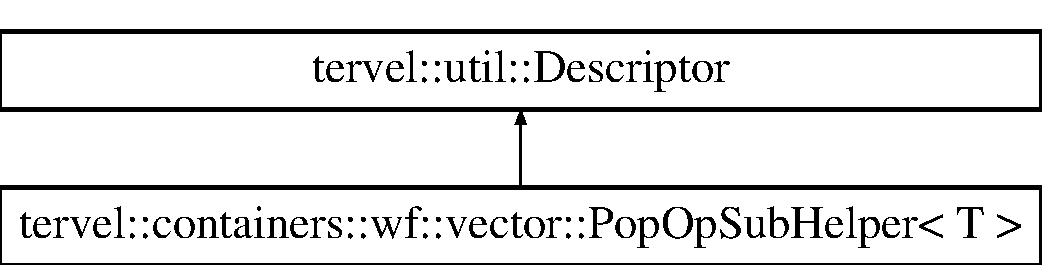
\includegraphics[height=2.000000cm]{classtervel_1_1containers_1_1wf_1_1vector_1_1_pop_op_sub_helper}
\end{center}
\end{figure}
\subsection*{Public Member Functions}
\begin{DoxyCompactItemize}
\item 
\hyperlink{classtervel_1_1containers_1_1wf_1_1vector_1_1_pop_op_sub_helper_a427afa23f9b23da97724a550956aac59}{Pop\+Op\+Sub\+Helper} (\hyperlink{classtervel_1_1containers_1_1wf_1_1vector_1_1_pop_op_helper}{Pop\+Op\+Helper}$<$ T $>$ $\ast$parent, T \hyperlink{classtervel_1_1containers_1_1wf_1_1vector_1_1_pop_op_sub_helper_a50f35566adc28c29e64593f3159aa96a}{val})
\item 
void \hyperlink{classtervel_1_1containers_1_1wf_1_1vector_1_1_pop_op_sub_helper_a50f35566adc28c29e64593f3159aa96a}{val} (T \&val)
\item 
void $\ast$ \hyperlink{classtervel_1_1containers_1_1wf_1_1vector_1_1_pop_op_sub_helper_a2b908a6e906f82a63af7e662fd6407cd}{get\+\_\+logical\+\_\+value} ()
\begin{DoxyCompactList}\small\item\em This method is implemented by each sub class. \end{DoxyCompactList}\item 
void $\ast$ \hyperlink{classtervel_1_1containers_1_1wf_1_1vector_1_1_pop_op_sub_helper_a8dc2729e8f7ed857c55df0f56361622b}{complete} (void $\ast$value, std\+::atomic$<$ void $\ast$ $>$ $\ast$address)
\begin{DoxyCompactList}\small\item\em This method is implemented by each sub class and must guarantee that upon return that the descriptor no longer exists at the address it was placed. \end{DoxyCompactList}\item 
bool \hyperlink{classtervel_1_1containers_1_1wf_1_1vector_1_1_pop_op_sub_helper_ae0fcfb9527874f0b321b0fd48a295833}{on\+\_\+watch} (std\+::atomic$<$ void $\ast$ $>$ $\ast$address, void $\ast$value)
\begin{DoxyCompactList}\small\item\em This method is optional to implement for each sub class. \end{DoxyCompactList}\end{DoxyCompactItemize}
\subsection*{Private Attributes}
\begin{DoxyCompactItemize}
\item 
T \hyperlink{classtervel_1_1containers_1_1wf_1_1vector_1_1_pop_op_sub_helper_a7957cf169b647bdad67fa9a577a6ebcf}{val\+\_\+}
\item 
\hyperlink{classtervel_1_1containers_1_1wf_1_1vector_1_1_pop_op_helper}{Pop\+Op\+Helper}$<$ T $>$ $\ast$ \hyperlink{classtervel_1_1containers_1_1wf_1_1vector_1_1_pop_op_sub_helper_a8026aadc97236024880ec507b252d7f8}{parent\+\_\+}
\end{DoxyCompactItemize}


\subsection{Constructor \& Destructor Documentation}
\hypertarget{classtervel_1_1containers_1_1wf_1_1vector_1_1_pop_op_sub_helper_a427afa23f9b23da97724a550956aac59}{}\index{tervel\+::containers\+::wf\+::vector\+::\+Pop\+Op\+Sub\+Helper@{tervel\+::containers\+::wf\+::vector\+::\+Pop\+Op\+Sub\+Helper}!Pop\+Op\+Sub\+Helper@{Pop\+Op\+Sub\+Helper}}
\index{Pop\+Op\+Sub\+Helper@{Pop\+Op\+Sub\+Helper}!tervel\+::containers\+::wf\+::vector\+::\+Pop\+Op\+Sub\+Helper@{tervel\+::containers\+::wf\+::vector\+::\+Pop\+Op\+Sub\+Helper}}
\subsubsection[{Pop\+Op\+Sub\+Helper(\+Pop\+Op\+Helper$<$ T $>$ $\ast$parent, T val)}]{\setlength{\rightskip}{0pt plus 5cm}template$<$typename T$>$ {\bf tervel\+::containers\+::wf\+::vector\+::\+Pop\+Op\+Sub\+Helper}$<$ T $>$\+::{\bf Pop\+Op\+Sub\+Helper} (
\begin{DoxyParamCaption}
\item[{{\bf Pop\+Op\+Helper}$<$ T $>$ $\ast$}]{parent, }
\item[{T}]{val}
\end{DoxyParamCaption}
)\hspace{0.3cm}{\ttfamily [inline]}, {\ttfamily [explicit]}}\label{classtervel_1_1containers_1_1wf_1_1vector_1_1_pop_op_sub_helper_a427afa23f9b23da97724a550956aac59}


\subsection{Member Function Documentation}
\hypertarget{classtervel_1_1containers_1_1wf_1_1vector_1_1_pop_op_sub_helper_a8dc2729e8f7ed857c55df0f56361622b}{}\index{tervel\+::containers\+::wf\+::vector\+::\+Pop\+Op\+Sub\+Helper@{tervel\+::containers\+::wf\+::vector\+::\+Pop\+Op\+Sub\+Helper}!complete@{complete}}
\index{complete@{complete}!tervel\+::containers\+::wf\+::vector\+::\+Pop\+Op\+Sub\+Helper@{tervel\+::containers\+::wf\+::vector\+::\+Pop\+Op\+Sub\+Helper}}
\subsubsection[{complete(void $\ast$value, std\+::atomic$<$ void $\ast$ $>$ $\ast$address)}]{\setlength{\rightskip}{0pt plus 5cm}template$<$typename T$>$ void$\ast$ {\bf tervel\+::containers\+::wf\+::vector\+::\+Pop\+Op\+Sub\+Helper}$<$ T $>$\+::complete (
\begin{DoxyParamCaption}
\item[{void $\ast$}]{current, }
\item[{std\+::atomic$<$ void $\ast$ $>$ $\ast$}]{address}
\end{DoxyParamCaption}
)\hspace{0.3cm}{\ttfamily [inline]}, {\ttfamily [virtual]}}\label{classtervel_1_1containers_1_1wf_1_1vector_1_1_pop_op_sub_helper_a8dc2729e8f7ed857c55df0f56361622b}


This method is implemented by each sub class and must guarantee that upon return that the descriptor no longer exists at the address it was placed. 


\begin{DoxyParams}{Parameters}
{\em current} & the reference to this object as it is at the address, \\
\hline
{\em address} & the location this object was read from \\
\hline
\end{DoxyParams}


Implements \hyperlink{classtervel_1_1util_1_1_descriptor_a4303b2a08e3ab67de5533cfb20db87c9}{tervel\+::util\+::\+Descriptor}.

\hypertarget{classtervel_1_1containers_1_1wf_1_1vector_1_1_pop_op_sub_helper_a2b908a6e906f82a63af7e662fd6407cd}{}\index{tervel\+::containers\+::wf\+::vector\+::\+Pop\+Op\+Sub\+Helper@{tervel\+::containers\+::wf\+::vector\+::\+Pop\+Op\+Sub\+Helper}!get\+\_\+logical\+\_\+value@{get\+\_\+logical\+\_\+value}}
\index{get\+\_\+logical\+\_\+value@{get\+\_\+logical\+\_\+value}!tervel\+::containers\+::wf\+::vector\+::\+Pop\+Op\+Sub\+Helper@{tervel\+::containers\+::wf\+::vector\+::\+Pop\+Op\+Sub\+Helper}}
\subsubsection[{get\+\_\+logical\+\_\+value()}]{\setlength{\rightskip}{0pt plus 5cm}template$<$typename T$>$ void$\ast$ {\bf tervel\+::containers\+::wf\+::vector\+::\+Pop\+Op\+Sub\+Helper}$<$ T $>$\+::get\+\_\+logical\+\_\+value (
\begin{DoxyParamCaption}
{}
\end{DoxyParamCaption}
)\hspace{0.3cm}{\ttfamily [inline]}, {\ttfamily [virtual]}}\label{classtervel_1_1containers_1_1wf_1_1vector_1_1_pop_op_sub_helper_a2b908a6e906f82a63af7e662fd6407cd}


This method is implemented by each sub class. 

It returns the logical value of the past address. If the associated operation is still in progress then it will generally return the value that was replaced by this descriptor. Otherwise it will generally return the result of the operation for the specified address.

It can only be called from the static function which protects the object from being reused during the function. 

Implements \hyperlink{classtervel_1_1util_1_1_descriptor_a5b443eeb6acf1207f27a6d06c39d4ad4}{tervel\+::util\+::\+Descriptor}.

\hypertarget{classtervel_1_1containers_1_1wf_1_1vector_1_1_pop_op_sub_helper_ae0fcfb9527874f0b321b0fd48a295833}{}\index{tervel\+::containers\+::wf\+::vector\+::\+Pop\+Op\+Sub\+Helper@{tervel\+::containers\+::wf\+::vector\+::\+Pop\+Op\+Sub\+Helper}!on\+\_\+watch@{on\+\_\+watch}}
\index{on\+\_\+watch@{on\+\_\+watch}!tervel\+::containers\+::wf\+::vector\+::\+Pop\+Op\+Sub\+Helper@{tervel\+::containers\+::wf\+::vector\+::\+Pop\+Op\+Sub\+Helper}}
\subsubsection[{on\+\_\+watch(std\+::atomic$<$ void $\ast$ $>$ $\ast$address, void $\ast$value)}]{\setlength{\rightskip}{0pt plus 5cm}template$<$typename T$>$ bool {\bf tervel\+::containers\+::wf\+::vector\+::\+Pop\+Op\+Sub\+Helper}$<$ T $>$\+::on\+\_\+watch (
\begin{DoxyParamCaption}
\item[{std\+::atomic$<$ void $\ast$ $>$ $\ast$}]{, }
\item[{void $\ast$}]{}
\end{DoxyParamCaption}
)\hspace{0.3cm}{\ttfamily [inline]}, {\ttfamily [virtual]}}\label{classtervel_1_1containers_1_1wf_1_1vector_1_1_pop_op_sub_helper_ae0fcfb9527874f0b321b0fd48a295833}


This method is optional to implement for each sub class. 

In the event there is a complex dependency between descriptor objects, where watching one implies performing other actions, such as watching a parent object, a developer will implement this function to encapsulate that logic

This function is called by the static watch function It should not watch itself.


\begin{DoxyParams}{Parameters}
{\em address} & The location to check. \\
\hline
{\em expected} & The expected value for that location\\
\hline
\end{DoxyParams}
\begin{DoxyReturn}{Returns}
true if successful, false otherwise 
\end{DoxyReturn}


Reimplemented from \hyperlink{classtervel_1_1util_1_1_descriptor_ab643e09f20f35149dc820766b0f9ccdb}{tervel\+::util\+::\+Descriptor}.

\hypertarget{classtervel_1_1containers_1_1wf_1_1vector_1_1_pop_op_sub_helper_a50f35566adc28c29e64593f3159aa96a}{}\index{tervel\+::containers\+::wf\+::vector\+::\+Pop\+Op\+Sub\+Helper@{tervel\+::containers\+::wf\+::vector\+::\+Pop\+Op\+Sub\+Helper}!val@{val}}
\index{val@{val}!tervel\+::containers\+::wf\+::vector\+::\+Pop\+Op\+Sub\+Helper@{tervel\+::containers\+::wf\+::vector\+::\+Pop\+Op\+Sub\+Helper}}
\subsubsection[{val(\+T \&val)}]{\setlength{\rightskip}{0pt plus 5cm}template$<$typename T$>$ void {\bf tervel\+::containers\+::wf\+::vector\+::\+Pop\+Op\+Sub\+Helper}$<$ T $>$\+::val (
\begin{DoxyParamCaption}
\item[{T \&}]{val}
\end{DoxyParamCaption}
)\hspace{0.3cm}{\ttfamily [inline]}}\label{classtervel_1_1containers_1_1wf_1_1vector_1_1_pop_op_sub_helper_a50f35566adc28c29e64593f3159aa96a}


\subsection{Member Data Documentation}
\hypertarget{classtervel_1_1containers_1_1wf_1_1vector_1_1_pop_op_sub_helper_a8026aadc97236024880ec507b252d7f8}{}\index{tervel\+::containers\+::wf\+::vector\+::\+Pop\+Op\+Sub\+Helper@{tervel\+::containers\+::wf\+::vector\+::\+Pop\+Op\+Sub\+Helper}!parent\+\_\+@{parent\+\_\+}}
\index{parent\+\_\+@{parent\+\_\+}!tervel\+::containers\+::wf\+::vector\+::\+Pop\+Op\+Sub\+Helper@{tervel\+::containers\+::wf\+::vector\+::\+Pop\+Op\+Sub\+Helper}}
\subsubsection[{parent\+\_\+}]{\setlength{\rightskip}{0pt plus 5cm}template$<$typename T$>$ {\bf Pop\+Op\+Helper}$<$T$>$$\ast$ {\bf tervel\+::containers\+::wf\+::vector\+::\+Pop\+Op\+Sub\+Helper}$<$ T $>$\+::parent\+\_\+\hspace{0.3cm}{\ttfamily [private]}}\label{classtervel_1_1containers_1_1wf_1_1vector_1_1_pop_op_sub_helper_a8026aadc97236024880ec507b252d7f8}
\hypertarget{classtervel_1_1containers_1_1wf_1_1vector_1_1_pop_op_sub_helper_a7957cf169b647bdad67fa9a577a6ebcf}{}\index{tervel\+::containers\+::wf\+::vector\+::\+Pop\+Op\+Sub\+Helper@{tervel\+::containers\+::wf\+::vector\+::\+Pop\+Op\+Sub\+Helper}!val\+\_\+@{val\+\_\+}}
\index{val\+\_\+@{val\+\_\+}!tervel\+::containers\+::wf\+::vector\+::\+Pop\+Op\+Sub\+Helper@{tervel\+::containers\+::wf\+::vector\+::\+Pop\+Op\+Sub\+Helper}}
\subsubsection[{val\+\_\+}]{\setlength{\rightskip}{0pt plus 5cm}template$<$typename T$>$ T {\bf tervel\+::containers\+::wf\+::vector\+::\+Pop\+Op\+Sub\+Helper}$<$ T $>$\+::val\+\_\+\hspace{0.3cm}{\ttfamily [private]}}\label{classtervel_1_1containers_1_1wf_1_1vector_1_1_pop_op_sub_helper_a7957cf169b647bdad67fa9a577a6ebcf}


The documentation for this class was generated from the following file\+:\begin{DoxyCompactItemize}
\item 
tervel/containers/wf/vector/\hyperlink{popback__op_8h}{popback\+\_\+op.\+h}\end{DoxyCompactItemize}

\hypertarget{class_pop_sub_helper}{}\section{Pop\+Sub\+Helper Class Reference}
\label{class_pop_sub_helper}\index{Pop\+Sub\+Helper@{Pop\+Sub\+Helper}}


{\ttfamily \#include $<$pop\+\_\+helper.\+h$>$}

Inheritance diagram for Pop\+Sub\+Helper\+:\begin{figure}[H]
\begin{center}
\leavevmode
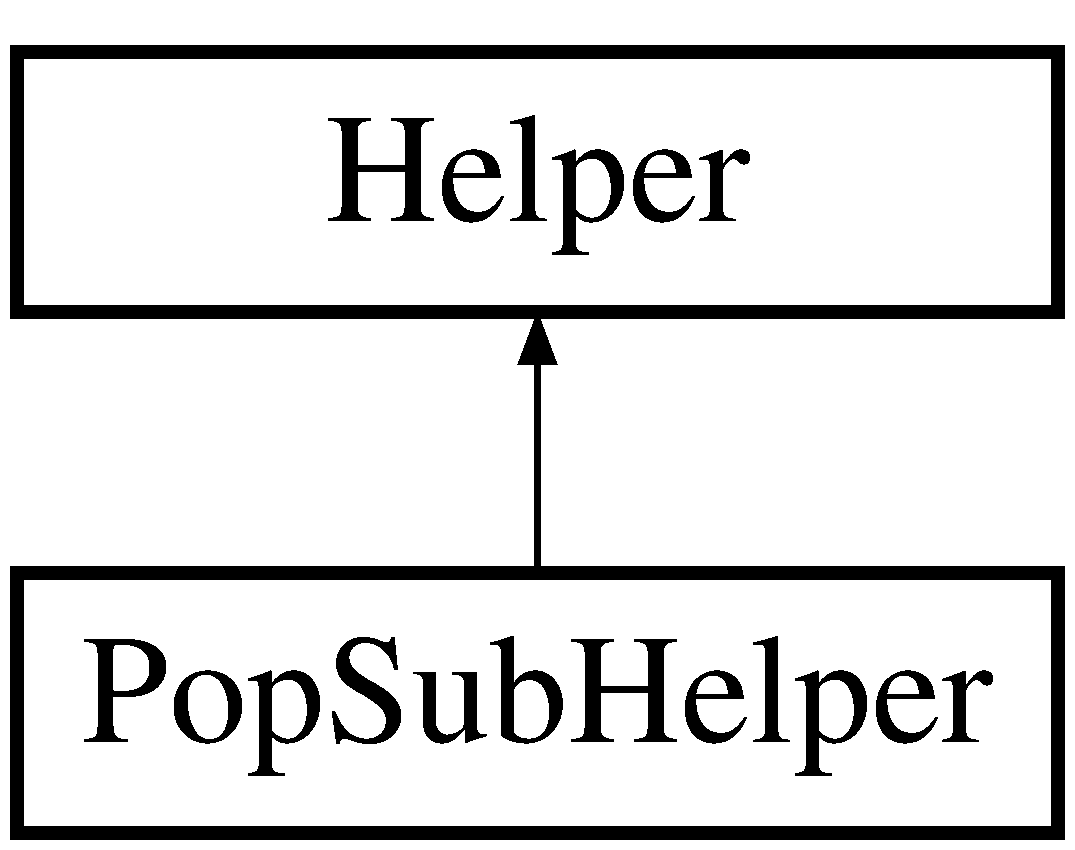
\includegraphics[height=2.000000cm]{class_pop_sub_helper}
\end{center}
\end{figure}
\subsection*{Public Member Functions}
\begin{DoxyCompactItemize}
\item 
void \hyperlink{class_pop_sub_helper_aa2830f2758975fb78e4d603ecf582092}{init} (\hyperlink{class_pop_helper}{Pop\+Helper} $\ast$p)
\item 
\hyperlink{class_pop_sub_helper_ad743a1ad146cc5a21a33300857b6989f}{Pop\+Sub\+Helper} (\hyperlink{class_pop_helper}{Pop\+Helper} $\ast$p)
\item 
void $\ast$ \hyperlink{class_pop_sub_helper_acbb3db6f8695be462af7d7e0a0853c9b}{get\+Value} ()
\item 
bool \hyperlink{class_pop_sub_helper_ae594014ef3cb91ecf55fa5d76eb2bf21}{complete} (W\+F\+Vector $\ast$vec, int pos)
\item 
bool \hyperlink{class_pop_sub_helper_ab3d196973dfda34200dcc16bce0b303b}{try\+Free} ()
\item 
bool \hyperlink{class_pop_sub_helper_ae4e86d5f4ba56ee2e0933f666964dcde}{watch} (void $\ast$p, Array\+Element $\ast$a)
\item 
void \hyperlink{class_pop_sub_helper_ac6b19047e3869d29875d8d8399f271cf}{unwatch} ()
\item 
bool \hyperlink{class_pop_sub_helper_a627522e3169aa505ac817cbe6d63d634}{is\+Watched} ()
\item 
void $\ast$ \hyperlink{class_pop_sub_helper_af568847074d4622ffdae03990ea83dfb}{read\+Through} ()
\end{DoxyCompactItemize}
\subsection*{Public Attributes}
\begin{DoxyCompactItemize}
\item 
void $\ast$ \hyperlink{class_pop_sub_helper_aed4ed06407d4fde68304918e1b9f0dcd}{value}
\item 
\hyperlink{class_pop_helper}{Pop\+Helper} $\ast$ \hyperlink{class_pop_sub_helper_ab5875762d6213bdc26bb7edee89c6a3a}{parent}
\end{DoxyCompactItemize}


\subsection{Constructor \& Destructor Documentation}
\hypertarget{class_pop_sub_helper_ad743a1ad146cc5a21a33300857b6989f}{}\index{Pop\+Sub\+Helper@{Pop\+Sub\+Helper}!Pop\+Sub\+Helper@{Pop\+Sub\+Helper}}
\index{Pop\+Sub\+Helper@{Pop\+Sub\+Helper}!Pop\+Sub\+Helper@{Pop\+Sub\+Helper}}
\subsubsection[{Pop\+Sub\+Helper(\+Pop\+Helper $\ast$p)}]{\setlength{\rightskip}{0pt plus 5cm}Pop\+Sub\+Helper\+::\+Pop\+Sub\+Helper (
\begin{DoxyParamCaption}
\item[{{\bf Pop\+Helper} $\ast$}]{p}
\end{DoxyParamCaption}
)\hspace{0.3cm}{\ttfamily [inline]}}\label{class_pop_sub_helper_ad743a1ad146cc5a21a33300857b6989f}


\subsection{Member Function Documentation}
\hypertarget{class_pop_sub_helper_ae594014ef3cb91ecf55fa5d76eb2bf21}{}\index{Pop\+Sub\+Helper@{Pop\+Sub\+Helper}!complete@{complete}}
\index{complete@{complete}!Pop\+Sub\+Helper@{Pop\+Sub\+Helper}}
\subsubsection[{complete(\+W\+F\+Vector $\ast$vec, int pos)}]{\setlength{\rightskip}{0pt plus 5cm}bool Pop\+Sub\+Helper\+::complete (
\begin{DoxyParamCaption}
\item[{W\+F\+Vector $\ast$}]{vec, }
\item[{int}]{pos}
\end{DoxyParamCaption}
)}\label{class_pop_sub_helper_ae594014ef3cb91ecf55fa5d76eb2bf21}
\hypertarget{class_pop_sub_helper_acbb3db6f8695be462af7d7e0a0853c9b}{}\index{Pop\+Sub\+Helper@{Pop\+Sub\+Helper}!get\+Value@{get\+Value}}
\index{get\+Value@{get\+Value}!Pop\+Sub\+Helper@{Pop\+Sub\+Helper}}
\subsubsection[{get\+Value()}]{\setlength{\rightskip}{0pt plus 5cm}void $\ast$ Pop\+Sub\+Helper\+::get\+Value (
\begin{DoxyParamCaption}
{}
\end{DoxyParamCaption}
)}\label{class_pop_sub_helper_acbb3db6f8695be462af7d7e0a0853c9b}
\hypertarget{class_pop_sub_helper_aa2830f2758975fb78e4d603ecf582092}{}\index{Pop\+Sub\+Helper@{Pop\+Sub\+Helper}!init@{init}}
\index{init@{init}!Pop\+Sub\+Helper@{Pop\+Sub\+Helper}}
\subsubsection[{init(\+Pop\+Helper $\ast$p)}]{\setlength{\rightskip}{0pt plus 5cm}void Pop\+Sub\+Helper\+::init (
\begin{DoxyParamCaption}
\item[{{\bf Pop\+Helper} $\ast$}]{p}
\end{DoxyParamCaption}
)\hspace{0.3cm}{\ttfamily [inline]}}\label{class_pop_sub_helper_aa2830f2758975fb78e4d603ecf582092}
\hypertarget{class_pop_sub_helper_a627522e3169aa505ac817cbe6d63d634}{}\index{Pop\+Sub\+Helper@{Pop\+Sub\+Helper}!is\+Watched@{is\+Watched}}
\index{is\+Watched@{is\+Watched}!Pop\+Sub\+Helper@{Pop\+Sub\+Helper}}
\subsubsection[{is\+Watched()}]{\setlength{\rightskip}{0pt plus 5cm}bool Pop\+Sub\+Helper\+::is\+Watched (
\begin{DoxyParamCaption}
{}
\end{DoxyParamCaption}
)\hspace{0.3cm}{\ttfamily [inline]}}\label{class_pop_sub_helper_a627522e3169aa505ac817cbe6d63d634}
\hypertarget{class_pop_sub_helper_af568847074d4622ffdae03990ea83dfb}{}\index{Pop\+Sub\+Helper@{Pop\+Sub\+Helper}!read\+Through@{read\+Through}}
\index{read\+Through@{read\+Through}!Pop\+Sub\+Helper@{Pop\+Sub\+Helper}}
\subsubsection[{read\+Through()}]{\setlength{\rightskip}{0pt plus 5cm}void$\ast$ Pop\+Sub\+Helper\+::read\+Through (
\begin{DoxyParamCaption}
{}
\end{DoxyParamCaption}
)\hspace{0.3cm}{\ttfamily [inline]}}\label{class_pop_sub_helper_af568847074d4622ffdae03990ea83dfb}
\hypertarget{class_pop_sub_helper_ab3d196973dfda34200dcc16bce0b303b}{}\index{Pop\+Sub\+Helper@{Pop\+Sub\+Helper}!try\+Free@{try\+Free}}
\index{try\+Free@{try\+Free}!Pop\+Sub\+Helper@{Pop\+Sub\+Helper}}
\subsubsection[{try\+Free()}]{\setlength{\rightskip}{0pt plus 5cm}bool Pop\+Sub\+Helper\+::try\+Free (
\begin{DoxyParamCaption}
{}
\end{DoxyParamCaption}
)}\label{class_pop_sub_helper_ab3d196973dfda34200dcc16bce0b303b}
\hypertarget{class_pop_sub_helper_ac6b19047e3869d29875d8d8399f271cf}{}\index{Pop\+Sub\+Helper@{Pop\+Sub\+Helper}!unwatch@{unwatch}}
\index{unwatch@{unwatch}!Pop\+Sub\+Helper@{Pop\+Sub\+Helper}}
\subsubsection[{unwatch()}]{\setlength{\rightskip}{0pt plus 5cm}void Pop\+Sub\+Helper\+::unwatch (
\begin{DoxyParamCaption}
{}
\end{DoxyParamCaption}
)\hspace{0.3cm}{\ttfamily [inline]}}\label{class_pop_sub_helper_ac6b19047e3869d29875d8d8399f271cf}
\hypertarget{class_pop_sub_helper_ae4e86d5f4ba56ee2e0933f666964dcde}{}\index{Pop\+Sub\+Helper@{Pop\+Sub\+Helper}!watch@{watch}}
\index{watch@{watch}!Pop\+Sub\+Helper@{Pop\+Sub\+Helper}}
\subsubsection[{watch(void $\ast$p, Array\+Element $\ast$a)}]{\setlength{\rightskip}{0pt plus 5cm}bool Pop\+Sub\+Helper\+::watch (
\begin{DoxyParamCaption}
\item[{void $\ast$}]{p, }
\item[{Array\+Element $\ast$}]{a}
\end{DoxyParamCaption}
)\hspace{0.3cm}{\ttfamily [inline]}}\label{class_pop_sub_helper_ae4e86d5f4ba56ee2e0933f666964dcde}


\subsection{Member Data Documentation}
\hypertarget{class_pop_sub_helper_ab5875762d6213bdc26bb7edee89c6a3a}{}\index{Pop\+Sub\+Helper@{Pop\+Sub\+Helper}!parent@{parent}}
\index{parent@{parent}!Pop\+Sub\+Helper@{Pop\+Sub\+Helper}}
\subsubsection[{parent}]{\setlength{\rightskip}{0pt plus 5cm}{\bf Pop\+Helper}$\ast$ Pop\+Sub\+Helper\+::parent}\label{class_pop_sub_helper_ab5875762d6213bdc26bb7edee89c6a3a}
\hypertarget{class_pop_sub_helper_aed4ed06407d4fde68304918e1b9f0dcd}{}\index{Pop\+Sub\+Helper@{Pop\+Sub\+Helper}!value@{value}}
\index{value@{value}!Pop\+Sub\+Helper@{Pop\+Sub\+Helper}}
\subsubsection[{value}]{\setlength{\rightskip}{0pt plus 5cm}void$\ast$ Pop\+Sub\+Helper\+::value}\label{class_pop_sub_helper_aed4ed06407d4fde68304918e1b9f0dcd}


The documentation for this class was generated from the following file\+:\begin{DoxyCompactItemize}
\item 
tervel/containers/wf/vector/old/\hyperlink{pop__helper_8h}{pop\+\_\+helper.\+h}\end{DoxyCompactItemize}

\hypertarget{classtervel_1_1containers_1_1wf_1_1vector_1_1_pop_w_r_a_op}{}\section{tervel\+:\+:containers\+:\+:wf\+:\+:vector\+:\+:Pop\+W\+R\+A\+Op$<$ T $>$ Class Template Reference}
\label{classtervel_1_1containers_1_1wf_1_1vector_1_1_pop_w_r_a_op}\index{tervel\+::containers\+::wf\+::vector\+::\+Pop\+W\+R\+A\+Op$<$ T $>$@{tervel\+::containers\+::wf\+::vector\+::\+Pop\+W\+R\+A\+Op$<$ T $>$}}


{\ttfamily \#include $<$popbackwra\+\_\+op.\+h$>$}

Inheritance diagram for tervel\+:\+:containers\+:\+:wf\+:\+:vector\+:\+:Pop\+W\+R\+A\+Op$<$ T $>$\+:\begin{figure}[H]
\begin{center}
\leavevmode
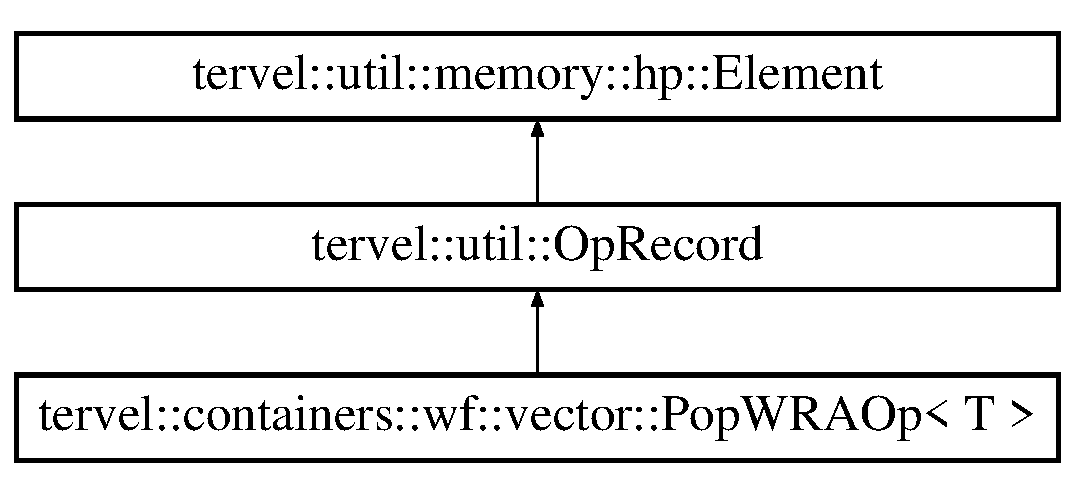
\includegraphics[height=3.000000cm]{classtervel_1_1containers_1_1wf_1_1vector_1_1_pop_w_r_a_op}
\end{center}
\end{figure}
\subsection*{Public Member Functions}
\begin{DoxyCompactItemize}
\item 
\hyperlink{classtervel_1_1containers_1_1wf_1_1vector_1_1_pop_w_r_a_op_acf35830bb35206909f2e65725848b2a0}{Pop\+W\+R\+A\+Op} (Vector$<$ T $>$ $\ast$vec)
\item 
\hyperlink{classtervel_1_1containers_1_1wf_1_1vector_1_1_pop_w_r_a_op_a8b7d9d55d71e5b322476dc0687c662ab}{$\sim$\+Pop\+W\+R\+A\+Op} ()
\item 
void \hyperlink{classtervel_1_1containers_1_1wf_1_1vector_1_1_pop_w_r_a_op_aaf425a7b0688f802c4ed134e8a5fc681}{set\+\_\+failed} ()
\item 
void \hyperlink{classtervel_1_1containers_1_1wf_1_1vector_1_1_pop_w_r_a_op_ab9dbcb928b3805f777856e2e35e9b461}{help\+\_\+complete} ()
\begin{DoxyCompactList}\small\item\em Implementations of this function that upon its return the operation described in the Op\+Record has been completed. \end{DoxyCompactList}\item 
bool \hyperlink{classtervel_1_1containers_1_1wf_1_1vector_1_1_pop_w_r_a_op_a3dcebe953f8462406063bbf98a9319f3}{result} (T \&val)
\item 
bool \hyperlink{classtervel_1_1containers_1_1wf_1_1vector_1_1_pop_w_r_a_op_ace647557e94685a3d0801f184c2e00e9}{result} ()
\end{DoxyCompactItemize}
\subsection*{Static Public Attributes}
\begin{DoxyCompactItemize}
\item 
static constexpr \hyperlink{classtervel_1_1containers_1_1wf_1_1vector_1_1_pop_w_r_a_op_helper}{Pop\+W\+R\+A\+Op\+Helper}$<$ T $>$ $\ast$ \hyperlink{classtervel_1_1containers_1_1wf_1_1vector_1_1_pop_w_r_a_op_ab59b382256b993e0bcae4c7a1064f665}{is\+\_\+empty\+\_\+const} \{reinterpret\+\_\+cast$<$\hyperlink{classtervel_1_1containers_1_1wf_1_1vector_1_1_pop_w_r_a_op_helper}{Pop\+W\+R\+A\+Op\+Helper}$<$T$>$ $\ast$$>$(0x1\+L)\}
\end{DoxyCompactItemize}
\subsection*{Private Attributes}
\begin{DoxyCompactItemize}
\item 
Vector$<$ T $>$ $\ast$ \hyperlink{classtervel_1_1containers_1_1wf_1_1vector_1_1_pop_w_r_a_op_ae0e8adc35df23f084d965aadc3f7de1b}{vec\+\_\+}
\item 
std\+::atomic$<$ T $>$ \hyperlink{classtervel_1_1containers_1_1wf_1_1vector_1_1_pop_w_r_a_op_a4b7f4c44861229e9388d0458a52da214}{value\+\_\+} \{Vector$<$T$>$\+::c\+\_\+not\+\_\+value\+\_\+\}
\item 
std\+::atomic$<$ T $>$ $\ast$ \hyperlink{classtervel_1_1containers_1_1wf_1_1vector_1_1_pop_w_r_a_op_af59ca2f59473f47e6bd91eb510a2db84}{prev\+\_\+spot\+\_\+} \{nullptr\}
\item 
std\+::atomic$<$ \hyperlink{classtervel_1_1containers_1_1wf_1_1vector_1_1_pop_w_r_a_op_helper}{Pop\+W\+R\+A\+Op\+Helper}$<$ T $>$ $\ast$ $>$ \hyperlink{classtervel_1_1containers_1_1wf_1_1vector_1_1_pop_w_r_a_op_ae3ba9949906f4848355163a3ca1f6185}{helper\+\_\+} \{nullptr\}
\end{DoxyCompactItemize}
\subsection*{Friends}
\begin{DoxyCompactItemize}
\item 
class \hyperlink{classtervel_1_1containers_1_1wf_1_1vector_1_1_pop_w_r_a_op_a001862caebce5469c52298be5fc100a3}{Pop\+W\+R\+A\+Op\+Helper$<$ T $>$}
\end{DoxyCompactItemize}


\subsection{Constructor \& Destructor Documentation}
\hypertarget{classtervel_1_1containers_1_1wf_1_1vector_1_1_pop_w_r_a_op_acf35830bb35206909f2e65725848b2a0}{}\index{tervel\+::containers\+::wf\+::vector\+::\+Pop\+W\+R\+A\+Op@{tervel\+::containers\+::wf\+::vector\+::\+Pop\+W\+R\+A\+Op}!Pop\+W\+R\+A\+Op@{Pop\+W\+R\+A\+Op}}
\index{Pop\+W\+R\+A\+Op@{Pop\+W\+R\+A\+Op}!tervel\+::containers\+::wf\+::vector\+::\+Pop\+W\+R\+A\+Op@{tervel\+::containers\+::wf\+::vector\+::\+Pop\+W\+R\+A\+Op}}
\subsubsection[{Pop\+W\+R\+A\+Op(\+Vector$<$ T $>$ $\ast$vec)}]{\setlength{\rightskip}{0pt plus 5cm}template$<$typename T$>$ {\bf tervel\+::containers\+::wf\+::vector\+::\+Pop\+W\+R\+A\+Op}$<$ T $>$\+::{\bf Pop\+W\+R\+A\+Op} (
\begin{DoxyParamCaption}
\item[{Vector$<$ T $>$ $\ast$}]{vec}
\end{DoxyParamCaption}
)\hspace{0.3cm}{\ttfamily [inline]}}\label{classtervel_1_1containers_1_1wf_1_1vector_1_1_pop_w_r_a_op_acf35830bb35206909f2e65725848b2a0}
\hypertarget{classtervel_1_1containers_1_1wf_1_1vector_1_1_pop_w_r_a_op_a8b7d9d55d71e5b322476dc0687c662ab}{}\index{tervel\+::containers\+::wf\+::vector\+::\+Pop\+W\+R\+A\+Op@{tervel\+::containers\+::wf\+::vector\+::\+Pop\+W\+R\+A\+Op}!````~Pop\+W\+R\+A\+Op@{$\sim$\+Pop\+W\+R\+A\+Op}}
\index{````~Pop\+W\+R\+A\+Op@{$\sim$\+Pop\+W\+R\+A\+Op}!tervel\+::containers\+::wf\+::vector\+::\+Pop\+W\+R\+A\+Op@{tervel\+::containers\+::wf\+::vector\+::\+Pop\+W\+R\+A\+Op}}
\subsubsection[{$\sim$\+Pop\+W\+R\+A\+Op()}]{\setlength{\rightskip}{0pt plus 5cm}template$<$typename T$>$ {\bf tervel\+::containers\+::wf\+::vector\+::\+Pop\+W\+R\+A\+Op}$<$ T $>$\+::$\sim${\bf Pop\+W\+R\+A\+Op} (
\begin{DoxyParamCaption}
{}
\end{DoxyParamCaption}
)\hspace{0.3cm}{\ttfamily [inline]}}\label{classtervel_1_1containers_1_1wf_1_1vector_1_1_pop_w_r_a_op_a8b7d9d55d71e5b322476dc0687c662ab}


\subsection{Member Function Documentation}
\hypertarget{classtervel_1_1containers_1_1wf_1_1vector_1_1_pop_w_r_a_op_ab9dbcb928b3805f777856e2e35e9b461}{}\index{tervel\+::containers\+::wf\+::vector\+::\+Pop\+W\+R\+A\+Op@{tervel\+::containers\+::wf\+::vector\+::\+Pop\+W\+R\+A\+Op}!help\+\_\+complete@{help\+\_\+complete}}
\index{help\+\_\+complete@{help\+\_\+complete}!tervel\+::containers\+::wf\+::vector\+::\+Pop\+W\+R\+A\+Op@{tervel\+::containers\+::wf\+::vector\+::\+Pop\+W\+R\+A\+Op}}
\subsubsection[{help\+\_\+complete()}]{\setlength{\rightskip}{0pt plus 5cm}template$<$typename T$>$ void {\bf tervel\+::containers\+::wf\+::vector\+::\+Pop\+W\+R\+A\+Op}$<$ T $>$\+::help\+\_\+complete (
\begin{DoxyParamCaption}
{}
\end{DoxyParamCaption}
)\hspace{0.3cm}{\ttfamily [inline]}, {\ttfamily [virtual]}}\label{classtervel_1_1containers_1_1wf_1_1vector_1_1_pop_w_r_a_op_ab9dbcb928b3805f777856e2e35e9b461}


Implementations of this function that upon its return the operation described in the Op\+Record has been completed. 

As such it must be thread-\/safe and the extending class must contain all the information necessary to complete the operation. 

Implements \hyperlink{classtervel_1_1util_1_1_op_record_aa75ab39688a8d4cceb6a1ef0409537c0}{tervel\+::util\+::\+Op\+Record}.

\hypertarget{classtervel_1_1containers_1_1wf_1_1vector_1_1_pop_w_r_a_op_a3dcebe953f8462406063bbf98a9319f3}{}\index{tervel\+::containers\+::wf\+::vector\+::\+Pop\+W\+R\+A\+Op@{tervel\+::containers\+::wf\+::vector\+::\+Pop\+W\+R\+A\+Op}!result@{result}}
\index{result@{result}!tervel\+::containers\+::wf\+::vector\+::\+Pop\+W\+R\+A\+Op@{tervel\+::containers\+::wf\+::vector\+::\+Pop\+W\+R\+A\+Op}}
\subsubsection[{result(\+T \&val)}]{\setlength{\rightskip}{0pt plus 5cm}template$<$typename T$>$ bool {\bf tervel\+::containers\+::wf\+::vector\+::\+Pop\+W\+R\+A\+Op}$<$ T $>$\+::result (
\begin{DoxyParamCaption}
\item[{T \&}]{val}
\end{DoxyParamCaption}
)\hspace{0.3cm}{\ttfamily [inline]}}\label{classtervel_1_1containers_1_1wf_1_1vector_1_1_pop_w_r_a_op_a3dcebe953f8462406063bbf98a9319f3}
\hypertarget{classtervel_1_1containers_1_1wf_1_1vector_1_1_pop_w_r_a_op_ace647557e94685a3d0801f184c2e00e9}{}\index{tervel\+::containers\+::wf\+::vector\+::\+Pop\+W\+R\+A\+Op@{tervel\+::containers\+::wf\+::vector\+::\+Pop\+W\+R\+A\+Op}!result@{result}}
\index{result@{result}!tervel\+::containers\+::wf\+::vector\+::\+Pop\+W\+R\+A\+Op@{tervel\+::containers\+::wf\+::vector\+::\+Pop\+W\+R\+A\+Op}}
\subsubsection[{result()}]{\setlength{\rightskip}{0pt plus 5cm}template$<$typename T$>$ bool {\bf tervel\+::containers\+::wf\+::vector\+::\+Pop\+W\+R\+A\+Op}$<$ T $>$\+::result (
\begin{DoxyParamCaption}
{}
\end{DoxyParamCaption}
)\hspace{0.3cm}{\ttfamily [inline]}}\label{classtervel_1_1containers_1_1wf_1_1vector_1_1_pop_w_r_a_op_ace647557e94685a3d0801f184c2e00e9}
\hypertarget{classtervel_1_1containers_1_1wf_1_1vector_1_1_pop_w_r_a_op_aaf425a7b0688f802c4ed134e8a5fc681}{}\index{tervel\+::containers\+::wf\+::vector\+::\+Pop\+W\+R\+A\+Op@{tervel\+::containers\+::wf\+::vector\+::\+Pop\+W\+R\+A\+Op}!set\+\_\+failed@{set\+\_\+failed}}
\index{set\+\_\+failed@{set\+\_\+failed}!tervel\+::containers\+::wf\+::vector\+::\+Pop\+W\+R\+A\+Op@{tervel\+::containers\+::wf\+::vector\+::\+Pop\+W\+R\+A\+Op}}
\subsubsection[{set\+\_\+failed()}]{\setlength{\rightskip}{0pt plus 5cm}template$<$typename T$>$ void {\bf tervel\+::containers\+::wf\+::vector\+::\+Pop\+W\+R\+A\+Op}$<$ T $>$\+::set\+\_\+failed (
\begin{DoxyParamCaption}
{}
\end{DoxyParamCaption}
)\hspace{0.3cm}{\ttfamily [inline]}}\label{classtervel_1_1containers_1_1wf_1_1vector_1_1_pop_w_r_a_op_aaf425a7b0688f802c4ed134e8a5fc681}


\subsection{Friends And Related Function Documentation}
\hypertarget{classtervel_1_1containers_1_1wf_1_1vector_1_1_pop_w_r_a_op_a001862caebce5469c52298be5fc100a3}{}\index{tervel\+::containers\+::wf\+::vector\+::\+Pop\+W\+R\+A\+Op@{tervel\+::containers\+::wf\+::vector\+::\+Pop\+W\+R\+A\+Op}!Pop\+W\+R\+A\+Op\+Helper$<$ T $>$@{Pop\+W\+R\+A\+Op\+Helper$<$ T $>$}}
\index{Pop\+W\+R\+A\+Op\+Helper$<$ T $>$@{Pop\+W\+R\+A\+Op\+Helper$<$ T $>$}!tervel\+::containers\+::wf\+::vector\+::\+Pop\+W\+R\+A\+Op@{tervel\+::containers\+::wf\+::vector\+::\+Pop\+W\+R\+A\+Op}}
\subsubsection[{Pop\+W\+R\+A\+Op\+Helper$<$ T $>$}]{\setlength{\rightskip}{0pt plus 5cm}template$<$typename T$>$ friend class {\bf Pop\+W\+R\+A\+Op\+Helper}$<$ T $>$\hspace{0.3cm}{\ttfamily [friend]}}\label{classtervel_1_1containers_1_1wf_1_1vector_1_1_pop_w_r_a_op_a001862caebce5469c52298be5fc100a3}


\subsection{Member Data Documentation}
\hypertarget{classtervel_1_1containers_1_1wf_1_1vector_1_1_pop_w_r_a_op_ae3ba9949906f4848355163a3ca1f6185}{}\index{tervel\+::containers\+::wf\+::vector\+::\+Pop\+W\+R\+A\+Op@{tervel\+::containers\+::wf\+::vector\+::\+Pop\+W\+R\+A\+Op}!helper\+\_\+@{helper\+\_\+}}
\index{helper\+\_\+@{helper\+\_\+}!tervel\+::containers\+::wf\+::vector\+::\+Pop\+W\+R\+A\+Op@{tervel\+::containers\+::wf\+::vector\+::\+Pop\+W\+R\+A\+Op}}
\subsubsection[{helper\+\_\+}]{\setlength{\rightskip}{0pt plus 5cm}template$<$typename T$>$ std\+::atomic$<${\bf Pop\+W\+R\+A\+Op\+Helper}$<$T$>$ $\ast$$>$ {\bf tervel\+::containers\+::wf\+::vector\+::\+Pop\+W\+R\+A\+Op}$<$ T $>$\+::helper\+\_\+ \{nullptr\}\hspace{0.3cm}{\ttfamily [private]}}\label{classtervel_1_1containers_1_1wf_1_1vector_1_1_pop_w_r_a_op_ae3ba9949906f4848355163a3ca1f6185}
\hypertarget{classtervel_1_1containers_1_1wf_1_1vector_1_1_pop_w_r_a_op_ab59b382256b993e0bcae4c7a1064f665}{}\index{tervel\+::containers\+::wf\+::vector\+::\+Pop\+W\+R\+A\+Op@{tervel\+::containers\+::wf\+::vector\+::\+Pop\+W\+R\+A\+Op}!is\+\_\+empty\+\_\+const@{is\+\_\+empty\+\_\+const}}
\index{is\+\_\+empty\+\_\+const@{is\+\_\+empty\+\_\+const}!tervel\+::containers\+::wf\+::vector\+::\+Pop\+W\+R\+A\+Op@{tervel\+::containers\+::wf\+::vector\+::\+Pop\+W\+R\+A\+Op}}
\subsubsection[{is\+\_\+empty\+\_\+const}]{\setlength{\rightskip}{0pt plus 5cm}template$<$typename T$>$ constexpr {\bf Pop\+W\+R\+A\+Op\+Helper}$<$T$>$$\ast$ {\bf tervel\+::containers\+::wf\+::vector\+::\+Pop\+W\+R\+A\+Op}$<$ T $>$\+::is\+\_\+empty\+\_\+const \{reinterpret\+\_\+cast$<${\bf Pop\+W\+R\+A\+Op\+Helper}$<$T$>$ $\ast$$>$(0x1\+L)\}\hspace{0.3cm}{\ttfamily [static]}}\label{classtervel_1_1containers_1_1wf_1_1vector_1_1_pop_w_r_a_op_ab59b382256b993e0bcae4c7a1064f665}
\hypertarget{classtervel_1_1containers_1_1wf_1_1vector_1_1_pop_w_r_a_op_af59ca2f59473f47e6bd91eb510a2db84}{}\index{tervel\+::containers\+::wf\+::vector\+::\+Pop\+W\+R\+A\+Op@{tervel\+::containers\+::wf\+::vector\+::\+Pop\+W\+R\+A\+Op}!prev\+\_\+spot\+\_\+@{prev\+\_\+spot\+\_\+}}
\index{prev\+\_\+spot\+\_\+@{prev\+\_\+spot\+\_\+}!tervel\+::containers\+::wf\+::vector\+::\+Pop\+W\+R\+A\+Op@{tervel\+::containers\+::wf\+::vector\+::\+Pop\+W\+R\+A\+Op}}
\subsubsection[{prev\+\_\+spot\+\_\+}]{\setlength{\rightskip}{0pt plus 5cm}template$<$typename T$>$ std\+::atomic$<$T$>$$\ast$ {\bf tervel\+::containers\+::wf\+::vector\+::\+Pop\+W\+R\+A\+Op}$<$ T $>$\+::prev\+\_\+spot\+\_\+ \{nullptr\}\hspace{0.3cm}{\ttfamily [private]}}\label{classtervel_1_1containers_1_1wf_1_1vector_1_1_pop_w_r_a_op_af59ca2f59473f47e6bd91eb510a2db84}
\hypertarget{classtervel_1_1containers_1_1wf_1_1vector_1_1_pop_w_r_a_op_a4b7f4c44861229e9388d0458a52da214}{}\index{tervel\+::containers\+::wf\+::vector\+::\+Pop\+W\+R\+A\+Op@{tervel\+::containers\+::wf\+::vector\+::\+Pop\+W\+R\+A\+Op}!value\+\_\+@{value\+\_\+}}
\index{value\+\_\+@{value\+\_\+}!tervel\+::containers\+::wf\+::vector\+::\+Pop\+W\+R\+A\+Op@{tervel\+::containers\+::wf\+::vector\+::\+Pop\+W\+R\+A\+Op}}
\subsubsection[{value\+\_\+}]{\setlength{\rightskip}{0pt plus 5cm}template$<$typename T$>$ std\+::atomic$<$T$>$ {\bf tervel\+::containers\+::wf\+::vector\+::\+Pop\+W\+R\+A\+Op}$<$ T $>$\+::value\+\_\+ \{Vector$<$T$>$\+::c\+\_\+not\+\_\+value\+\_\+\}\hspace{0.3cm}{\ttfamily [private]}}\label{classtervel_1_1containers_1_1wf_1_1vector_1_1_pop_w_r_a_op_a4b7f4c44861229e9388d0458a52da214}
\hypertarget{classtervel_1_1containers_1_1wf_1_1vector_1_1_pop_w_r_a_op_ae0e8adc35df23f084d965aadc3f7de1b}{}\index{tervel\+::containers\+::wf\+::vector\+::\+Pop\+W\+R\+A\+Op@{tervel\+::containers\+::wf\+::vector\+::\+Pop\+W\+R\+A\+Op}!vec\+\_\+@{vec\+\_\+}}
\index{vec\+\_\+@{vec\+\_\+}!tervel\+::containers\+::wf\+::vector\+::\+Pop\+W\+R\+A\+Op@{tervel\+::containers\+::wf\+::vector\+::\+Pop\+W\+R\+A\+Op}}
\subsubsection[{vec\+\_\+}]{\setlength{\rightskip}{0pt plus 5cm}template$<$typename T$>$ Vector$<$T$>$$\ast$ {\bf tervel\+::containers\+::wf\+::vector\+::\+Pop\+W\+R\+A\+Op}$<$ T $>$\+::vec\+\_\+\hspace{0.3cm}{\ttfamily [private]}}\label{classtervel_1_1containers_1_1wf_1_1vector_1_1_pop_w_r_a_op_ae0e8adc35df23f084d965aadc3f7de1b}


The documentation for this class was generated from the following file\+:\begin{DoxyCompactItemize}
\item 
tervel/containers/wf/vector/\hyperlink{popbackwra__op_8h}{popbackwra\+\_\+op.\+h}\end{DoxyCompactItemize}

\hypertarget{classtervel_1_1containers_1_1wf_1_1vector_1_1_pop_w_r_a_op_helper}{}\section{tervel\+:\+:containers\+:\+:wf\+:\+:vector\+:\+:Pop\+W\+R\+A\+Op\+Helper$<$ T $>$ Class Template Reference}
\label{classtervel_1_1containers_1_1wf_1_1vector_1_1_pop_w_r_a_op_helper}\index{tervel\+::containers\+::wf\+::vector\+::\+Pop\+W\+R\+A\+Op\+Helper$<$ T $>$@{tervel\+::containers\+::wf\+::vector\+::\+Pop\+W\+R\+A\+Op\+Helper$<$ T $>$}}


{\ttfamily \#include $<$popbackwra\+\_\+op.\+h$>$}

Inheritance diagram for tervel\+:\+:containers\+:\+:wf\+:\+:vector\+:\+:Pop\+W\+R\+A\+Op\+Helper$<$ T $>$\+:\begin{figure}[H]
\begin{center}
\leavevmode
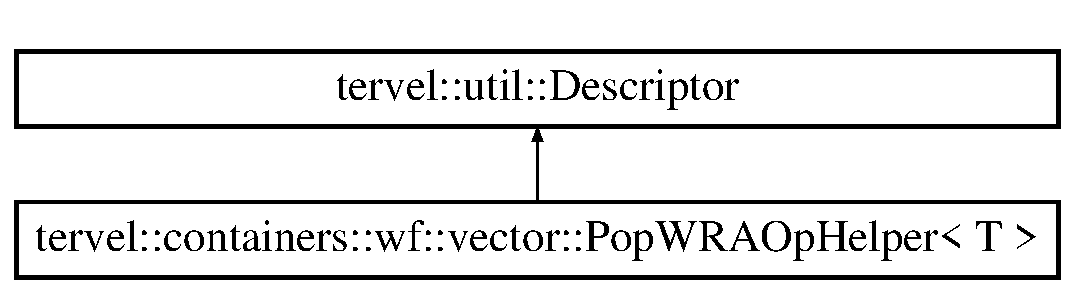
\includegraphics[height=2.000000cm]{classtervel_1_1containers_1_1wf_1_1vector_1_1_pop_w_r_a_op_helper}
\end{center}
\end{figure}
\subsection*{Public Member Functions}
\begin{DoxyCompactItemize}
\item 
\hyperlink{classtervel_1_1containers_1_1wf_1_1vector_1_1_pop_w_r_a_op_helper_a8347d7f3785c1bdbad3c865df59112fa}{Pop\+W\+R\+A\+Op\+Helper} (\hyperlink{classtervel_1_1containers_1_1wf_1_1vector_1_1_pop_w_r_a_op}{Pop\+W\+R\+A\+Op}$<$ T $>$ $\ast$op, T val)
\item 
\hyperlink{classtervel_1_1containers_1_1wf_1_1vector_1_1_pop_w_r_a_op_helper_aaece596129aece6c4a863a86eac19286}{$\sim$\+Pop\+W\+R\+A\+Op\+Helper} ()
\item 
void $\ast$ \hyperlink{classtervel_1_1containers_1_1wf_1_1vector_1_1_pop_w_r_a_op_helper_a4bb595dabd2cb32dc4171d82532c3413}{complete} (void $\ast$value, std\+::atomic$<$ void $\ast$ $>$ $\ast$address)
\begin{DoxyCompactList}\small\item\em This method is implemented by each sub class and must guarantee that upon return that the descriptor no longer exists at the address it was placed. \end{DoxyCompactList}\item 
bool \hyperlink{classtervel_1_1containers_1_1wf_1_1vector_1_1_pop_w_r_a_op_helper_a7290b783b392f57b6ef8195760a6abc0}{associate} ()
\item 
bool \hyperlink{classtervel_1_1containers_1_1wf_1_1vector_1_1_pop_w_r_a_op_helper_a1fcab473237a5d55a7389e6c8c871e2a}{result} (T \&val)
\item 
bool \hyperlink{classtervel_1_1containers_1_1wf_1_1vector_1_1_pop_w_r_a_op_helper_a3e8b506ad4e63de9f976f2057a0135d9}{result} ()
\end{DoxyCompactItemize}
\subsection*{Private Attributes}
\begin{DoxyCompactItemize}
\item 
T \hyperlink{classtervel_1_1containers_1_1wf_1_1vector_1_1_pop_w_r_a_op_helper_a8c2f74c19e182245e328b2dca7eeddfc}{val\+\_\+}
\item 
\hyperlink{classtervel_1_1containers_1_1wf_1_1vector_1_1_pop_w_r_a_op}{Pop\+W\+R\+A\+Op}$<$ T $>$ $\ast$ \hyperlink{classtervel_1_1containers_1_1wf_1_1vector_1_1_pop_w_r_a_op_helper_a5df18414ef72fae9e29b697287d5400f}{op\+\_\+} \{nullptr\}
\end{DoxyCompactItemize}


\subsection{Constructor \& Destructor Documentation}
\hypertarget{classtervel_1_1containers_1_1wf_1_1vector_1_1_pop_w_r_a_op_helper_a8347d7f3785c1bdbad3c865df59112fa}{}\index{tervel\+::containers\+::wf\+::vector\+::\+Pop\+W\+R\+A\+Op\+Helper@{tervel\+::containers\+::wf\+::vector\+::\+Pop\+W\+R\+A\+Op\+Helper}!Pop\+W\+R\+A\+Op\+Helper@{Pop\+W\+R\+A\+Op\+Helper}}
\index{Pop\+W\+R\+A\+Op\+Helper@{Pop\+W\+R\+A\+Op\+Helper}!tervel\+::containers\+::wf\+::vector\+::\+Pop\+W\+R\+A\+Op\+Helper@{tervel\+::containers\+::wf\+::vector\+::\+Pop\+W\+R\+A\+Op\+Helper}}
\subsubsection[{Pop\+W\+R\+A\+Op\+Helper(\+Pop\+W\+R\+A\+Op$<$ T $>$ $\ast$op, T val)}]{\setlength{\rightskip}{0pt plus 5cm}template$<$typename T$>$ {\bf tervel\+::containers\+::wf\+::vector\+::\+Pop\+W\+R\+A\+Op\+Helper}$<$ T $>$\+::{\bf Pop\+W\+R\+A\+Op\+Helper} (
\begin{DoxyParamCaption}
\item[{{\bf Pop\+W\+R\+A\+Op}$<$ T $>$ $\ast$}]{op, }
\item[{T}]{val}
\end{DoxyParamCaption}
)\hspace{0.3cm}{\ttfamily [inline]}}\label{classtervel_1_1containers_1_1wf_1_1vector_1_1_pop_w_r_a_op_helper_a8347d7f3785c1bdbad3c865df59112fa}
\hypertarget{classtervel_1_1containers_1_1wf_1_1vector_1_1_pop_w_r_a_op_helper_aaece596129aece6c4a863a86eac19286}{}\index{tervel\+::containers\+::wf\+::vector\+::\+Pop\+W\+R\+A\+Op\+Helper@{tervel\+::containers\+::wf\+::vector\+::\+Pop\+W\+R\+A\+Op\+Helper}!````~Pop\+W\+R\+A\+Op\+Helper@{$\sim$\+Pop\+W\+R\+A\+Op\+Helper}}
\index{````~Pop\+W\+R\+A\+Op\+Helper@{$\sim$\+Pop\+W\+R\+A\+Op\+Helper}!tervel\+::containers\+::wf\+::vector\+::\+Pop\+W\+R\+A\+Op\+Helper@{tervel\+::containers\+::wf\+::vector\+::\+Pop\+W\+R\+A\+Op\+Helper}}
\subsubsection[{$\sim$\+Pop\+W\+R\+A\+Op\+Helper()}]{\setlength{\rightskip}{0pt plus 5cm}template$<$typename T$>$ {\bf tervel\+::containers\+::wf\+::vector\+::\+Pop\+W\+R\+A\+Op\+Helper}$<$ T $>$\+::$\sim${\bf Pop\+W\+R\+A\+Op\+Helper} (
\begin{DoxyParamCaption}
{}
\end{DoxyParamCaption}
)\hspace{0.3cm}{\ttfamily [inline]}}\label{classtervel_1_1containers_1_1wf_1_1vector_1_1_pop_w_r_a_op_helper_aaece596129aece6c4a863a86eac19286}


\subsection{Member Function Documentation}
\hypertarget{classtervel_1_1containers_1_1wf_1_1vector_1_1_pop_w_r_a_op_helper_a7290b783b392f57b6ef8195760a6abc0}{}\index{tervel\+::containers\+::wf\+::vector\+::\+Pop\+W\+R\+A\+Op\+Helper@{tervel\+::containers\+::wf\+::vector\+::\+Pop\+W\+R\+A\+Op\+Helper}!associate@{associate}}
\index{associate@{associate}!tervel\+::containers\+::wf\+::vector\+::\+Pop\+W\+R\+A\+Op\+Helper@{tervel\+::containers\+::wf\+::vector\+::\+Pop\+W\+R\+A\+Op\+Helper}}
\subsubsection[{associate()}]{\setlength{\rightskip}{0pt plus 5cm}template$<$typename T$>$ bool {\bf tervel\+::containers\+::wf\+::vector\+::\+Pop\+W\+R\+A\+Op\+Helper}$<$ T $>$\+::associate (
\begin{DoxyParamCaption}
{}
\end{DoxyParamCaption}
)\hspace{0.3cm}{\ttfamily [inline]}}\label{classtervel_1_1containers_1_1wf_1_1vector_1_1_pop_w_r_a_op_helper_a7290b783b392f57b6ef8195760a6abc0}
\hypertarget{classtervel_1_1containers_1_1wf_1_1vector_1_1_pop_w_r_a_op_helper_a4bb595dabd2cb32dc4171d82532c3413}{}\index{tervel\+::containers\+::wf\+::vector\+::\+Pop\+W\+R\+A\+Op\+Helper@{tervel\+::containers\+::wf\+::vector\+::\+Pop\+W\+R\+A\+Op\+Helper}!complete@{complete}}
\index{complete@{complete}!tervel\+::containers\+::wf\+::vector\+::\+Pop\+W\+R\+A\+Op\+Helper@{tervel\+::containers\+::wf\+::vector\+::\+Pop\+W\+R\+A\+Op\+Helper}}
\subsubsection[{complete(void $\ast$value, std\+::atomic$<$ void $\ast$ $>$ $\ast$address)}]{\setlength{\rightskip}{0pt plus 5cm}template$<$typename T$>$ void$\ast$ {\bf tervel\+::containers\+::wf\+::vector\+::\+Pop\+W\+R\+A\+Op\+Helper}$<$ T $>$\+::complete (
\begin{DoxyParamCaption}
\item[{void $\ast$}]{current, }
\item[{std\+::atomic$<$ void $\ast$ $>$ $\ast$}]{address}
\end{DoxyParamCaption}
)\hspace{0.3cm}{\ttfamily [inline]}, {\ttfamily [virtual]}}\label{classtervel_1_1containers_1_1wf_1_1vector_1_1_pop_w_r_a_op_helper_a4bb595dabd2cb32dc4171d82532c3413}


This method is implemented by each sub class and must guarantee that upon return that the descriptor no longer exists at the address it was placed. 


\begin{DoxyParams}{Parameters}
{\em current} & the reference to this object as it is at the address, \\
\hline
{\em address} & the location this object was read from \\
\hline
\end{DoxyParams}


Implements \hyperlink{classtervel_1_1util_1_1_descriptor_a4303b2a08e3ab67de5533cfb20db87c9}{tervel\+::util\+::\+Descriptor}.

\hypertarget{classtervel_1_1containers_1_1wf_1_1vector_1_1_pop_w_r_a_op_helper_a1fcab473237a5d55a7389e6c8c871e2a}{}\index{tervel\+::containers\+::wf\+::vector\+::\+Pop\+W\+R\+A\+Op\+Helper@{tervel\+::containers\+::wf\+::vector\+::\+Pop\+W\+R\+A\+Op\+Helper}!result@{result}}
\index{result@{result}!tervel\+::containers\+::wf\+::vector\+::\+Pop\+W\+R\+A\+Op\+Helper@{tervel\+::containers\+::wf\+::vector\+::\+Pop\+W\+R\+A\+Op\+Helper}}
\subsubsection[{result(\+T \&val)}]{\setlength{\rightskip}{0pt plus 5cm}template$<$typename T$>$ bool {\bf tervel\+::containers\+::wf\+::vector\+::\+Pop\+W\+R\+A\+Op\+Helper}$<$ T $>$\+::result (
\begin{DoxyParamCaption}
\item[{T \&}]{val}
\end{DoxyParamCaption}
)\hspace{0.3cm}{\ttfamily [inline]}}\label{classtervel_1_1containers_1_1wf_1_1vector_1_1_pop_w_r_a_op_helper_a1fcab473237a5d55a7389e6c8c871e2a}
\hypertarget{classtervel_1_1containers_1_1wf_1_1vector_1_1_pop_w_r_a_op_helper_a3e8b506ad4e63de9f976f2057a0135d9}{}\index{tervel\+::containers\+::wf\+::vector\+::\+Pop\+W\+R\+A\+Op\+Helper@{tervel\+::containers\+::wf\+::vector\+::\+Pop\+W\+R\+A\+Op\+Helper}!result@{result}}
\index{result@{result}!tervel\+::containers\+::wf\+::vector\+::\+Pop\+W\+R\+A\+Op\+Helper@{tervel\+::containers\+::wf\+::vector\+::\+Pop\+W\+R\+A\+Op\+Helper}}
\subsubsection[{result()}]{\setlength{\rightskip}{0pt plus 5cm}template$<$typename T$>$ bool {\bf tervel\+::containers\+::wf\+::vector\+::\+Pop\+W\+R\+A\+Op\+Helper}$<$ T $>$\+::result (
\begin{DoxyParamCaption}
{}
\end{DoxyParamCaption}
)\hspace{0.3cm}{\ttfamily [inline]}}\label{classtervel_1_1containers_1_1wf_1_1vector_1_1_pop_w_r_a_op_helper_a3e8b506ad4e63de9f976f2057a0135d9}


\subsection{Member Data Documentation}
\hypertarget{classtervel_1_1containers_1_1wf_1_1vector_1_1_pop_w_r_a_op_helper_a5df18414ef72fae9e29b697287d5400f}{}\index{tervel\+::containers\+::wf\+::vector\+::\+Pop\+W\+R\+A\+Op\+Helper@{tervel\+::containers\+::wf\+::vector\+::\+Pop\+W\+R\+A\+Op\+Helper}!op\+\_\+@{op\+\_\+}}
\index{op\+\_\+@{op\+\_\+}!tervel\+::containers\+::wf\+::vector\+::\+Pop\+W\+R\+A\+Op\+Helper@{tervel\+::containers\+::wf\+::vector\+::\+Pop\+W\+R\+A\+Op\+Helper}}
\subsubsection[{op\+\_\+}]{\setlength{\rightskip}{0pt plus 5cm}template$<$typename T$>$ {\bf Pop\+W\+R\+A\+Op}$<$T$>$$\ast$ {\bf tervel\+::containers\+::wf\+::vector\+::\+Pop\+W\+R\+A\+Op\+Helper}$<$ T $>$\+::op\+\_\+ \{nullptr\}\hspace{0.3cm}{\ttfamily [private]}}\label{classtervel_1_1containers_1_1wf_1_1vector_1_1_pop_w_r_a_op_helper_a5df18414ef72fae9e29b697287d5400f}
\hypertarget{classtervel_1_1containers_1_1wf_1_1vector_1_1_pop_w_r_a_op_helper_a8c2f74c19e182245e328b2dca7eeddfc}{}\index{tervel\+::containers\+::wf\+::vector\+::\+Pop\+W\+R\+A\+Op\+Helper@{tervel\+::containers\+::wf\+::vector\+::\+Pop\+W\+R\+A\+Op\+Helper}!val\+\_\+@{val\+\_\+}}
\index{val\+\_\+@{val\+\_\+}!tervel\+::containers\+::wf\+::vector\+::\+Pop\+W\+R\+A\+Op\+Helper@{tervel\+::containers\+::wf\+::vector\+::\+Pop\+W\+R\+A\+Op\+Helper}}
\subsubsection[{val\+\_\+}]{\setlength{\rightskip}{0pt plus 5cm}template$<$typename T$>$ T {\bf tervel\+::containers\+::wf\+::vector\+::\+Pop\+W\+R\+A\+Op\+Helper}$<$ T $>$\+::val\+\_\+\hspace{0.3cm}{\ttfamily [private]}}\label{classtervel_1_1containers_1_1wf_1_1vector_1_1_pop_w_r_a_op_helper_a8c2f74c19e182245e328b2dca7eeddfc}


The documentation for this class was generated from the following file\+:\begin{DoxyCompactItemize}
\item 
tervel/containers/wf/vector/\hyperlink{popbackwra__op_8h}{popbackwra\+\_\+op.\+h}\end{DoxyCompactItemize}

\hypertarget{classtervel_1_1util_1_1_progress_assurance}{}\section{tervel\+:\+:util\+:\+:Progress\+Assurance Class Reference}
\label{classtervel_1_1util_1_1_progress_assurance}\index{tervel\+::util\+::\+Progress\+Assurance@{tervel\+::util\+::\+Progress\+Assurance}}


This class represents the progress assurance scheme employed by our library.  




{\ttfamily \#include $<$progress\+\_\+assurance.\+h$>$}

\subsection*{Classes}
\begin{DoxyCompactItemize}
\item 
class \hyperlink{classtervel_1_1util_1_1_progress_assurance_1_1_limit}{Limit}
\end{DoxyCompactItemize}
\subsection*{Public Member Functions}
\begin{DoxyCompactItemize}
\item 
\hyperlink{classtervel_1_1util_1_1_progress_assurance_a4e76edc1f1eb6b0b0111fbd2b5b73cb7}{Progress\+Assurance} (size\+\_\+t num\+\_\+threads)
\end{DoxyCompactItemize}
\subsection*{Static Public Member Functions}
\begin{DoxyCompactItemize}
\item 
static void \hyperlink{classtervel_1_1util_1_1_progress_assurance_ada9868a602d3f45d1c041a29a7612138}{check\+\_\+for\+\_\+announcement} (\hyperlink{classtervel_1_1util_1_1_progress_assurance}{Progress\+Assurance} $\ast$const progress\+\_\+assuarance=nullptr)
\begin{DoxyCompactList}\small\item\em This function checks at most one position in the op\+\_\+table\+\_\+ for an O\+P\+Recod If one is found it will call its help\+\_\+complete function. \end{DoxyCompactList}\item 
static void \hyperlink{classtervel_1_1util_1_1_progress_assurance_aa07f6bcc8e41c4c63066989f1ff90685}{make\+\_\+announcement} (\hyperlink{classtervel_1_1util_1_1_op_record}{Op\+Record} $\ast$op, const uint64\+\_\+t tid=\hyperlink{namespacetervel_a60b23602adbb2dee6160af411b74bfd3}{tervel\+::tl\+\_\+thread\+\_\+info}-\/$>$get\+\_\+thread\+\_\+id(), \hyperlink{classtervel_1_1util_1_1_progress_assurance}{Progress\+Assurance} $\ast$const prog\+\_\+assur=\hyperlink{namespacetervel_a60b23602adbb2dee6160af411b74bfd3}{tervel\+::tl\+\_\+thread\+\_\+info}-\/$>$get\+\_\+progress\+\_\+assurance())
\begin{DoxyCompactList}\small\item\em This function places the. \end{DoxyCompactList}\end{DoxyCompactItemize}
\subsection*{Static Public Attributes}
\begin{DoxyCompactItemize}
\item 
static constexpr size\+\_\+t \hyperlink{classtervel_1_1util_1_1_progress_assurance_a7b1a1448c14b614503aff9312593c9bc}{H\+E\+L\+P\+\_\+\+D\+E\+L\+A\+Y} = \hyperlink{util_8h_a5200ffa9857ce73ef77b3e8581d5b0cc}{T\+E\+R\+V\+E\+L\+\_\+\+P\+R\+O\+G\+\_\+\+A\+S\+S\+U\+R\+\_\+\+D\+E\+L\+A\+Y}
\begin{DoxyCompactList}\small\item\em Const used to delay an announcement. \end{DoxyCompactList}\end{DoxyCompactItemize}
\subsection*{Private Member Functions}
\begin{DoxyCompactItemize}
\item 
void \hyperlink{classtervel_1_1util_1_1_progress_assurance_af7f57b0721b40d5269416b6b8e5042f0}{p\+\_\+check\+\_\+for\+\_\+announcement} (size\+\_\+t \&hpos)
\begin{DoxyCompactList}\small\item\em This function checks at most one position in the op\+\_\+table\+\_\+ for an O\+P\+Recod If one is found it will call its help\+\_\+complete function. \end{DoxyCompactList}\item 
void \hyperlink{classtervel_1_1util_1_1_progress_assurance_a63193bc7abbdee5f81eef05986fc1c3e}{p\+\_\+make\+\_\+announcement} (\hyperlink{classtervel_1_1util_1_1_op_record}{Op\+Record} $\ast$op, const uint64\+\_\+t tid=\hyperlink{namespacetervel_a60b23602adbb2dee6160af411b74bfd3}{tervel\+::tl\+\_\+thread\+\_\+info}-\/$>$get\+\_\+thread\+\_\+id())
\begin{DoxyCompactList}\small\item\em This function places the. \end{DoxyCompactList}\item 
\hyperlink{classtervel_1_1util_1_1_progress_assurance_a923eb2780489a1bebb342c8fce904308}{D\+I\+S\+A\+L\+L\+O\+W\+\_\+\+C\+O\+P\+Y\+\_\+\+A\+N\+D\+\_\+\+A\+S\+S\+I\+G\+N} (\hyperlink{classtervel_1_1util_1_1_progress_assurance}{Progress\+Assurance})
\end{DoxyCompactItemize}
\subsection*{Private Attributes}
\begin{DoxyCompactItemize}
\item 
std\+::unique\+\_\+ptr$<$ std\+::atomic$<$ \hyperlink{classtervel_1_1util_1_1_op_record}{Op\+Record} $\ast$ $>$\mbox{[}$\,$\mbox{]}$>$ \hyperlink{classtervel_1_1util_1_1_progress_assurance_a7db95582f6fda286d62000d65963a926}{op\+\_\+table\+\_\+}
\begin{DoxyCompactList}\small\item\em Table for storing operation records, each thread has its own position that corresponds to its thread if. \end{DoxyCompactList}\item 
const size\+\_\+t \hyperlink{classtervel_1_1util_1_1_progress_assurance_a33770716cc5c51b06474d3a108992efb}{num\+\_\+threads\+\_\+}
\begin{DoxyCompactList}\small\item\em The number of threads that are using this operation table. \end{DoxyCompactList}\end{DoxyCompactItemize}


\subsection{Detailed Description}
This class represents the progress assurance scheme employed by our library. 

For this scheme to be effective, each operation which may indefinitely prevent the progress of some other operation must call the static function offer\+\_\+help This ensures that if a thread is continually failing its operation, then after a finite number of tries all thread will be helping. The number of failures is M\+A\+X\+\_\+\+F\+A\+I\+L\+U\+R\+E\+S + (number of threads$^\wedge$2)$\ast$ help\+\_\+delay 

\subsection{Constructor \& Destructor Documentation}
\hypertarget{classtervel_1_1util_1_1_progress_assurance_a4e76edc1f1eb6b0b0111fbd2b5b73cb7}{}\index{tervel\+::util\+::\+Progress\+Assurance@{tervel\+::util\+::\+Progress\+Assurance}!Progress\+Assurance@{Progress\+Assurance}}
\index{Progress\+Assurance@{Progress\+Assurance}!tervel\+::util\+::\+Progress\+Assurance@{tervel\+::util\+::\+Progress\+Assurance}}
\subsubsection[{Progress\+Assurance(size\+\_\+t num\+\_\+threads)}]{\setlength{\rightskip}{0pt plus 5cm}tervel\+::util\+::\+Progress\+Assurance\+::\+Progress\+Assurance (
\begin{DoxyParamCaption}
\item[{size\+\_\+t}]{num\+\_\+threads}
\end{DoxyParamCaption}
)\hspace{0.3cm}{\ttfamily [inline]}, {\ttfamily [explicit]}}\label{classtervel_1_1util_1_1_progress_assurance_a4e76edc1f1eb6b0b0111fbd2b5b73cb7}


\subsection{Member Function Documentation}
\hypertarget{classtervel_1_1util_1_1_progress_assurance_ada9868a602d3f45d1c041a29a7612138}{}\index{tervel\+::util\+::\+Progress\+Assurance@{tervel\+::util\+::\+Progress\+Assurance}!check\+\_\+for\+\_\+announcement@{check\+\_\+for\+\_\+announcement}}
\index{check\+\_\+for\+\_\+announcement@{check\+\_\+for\+\_\+announcement}!tervel\+::util\+::\+Progress\+Assurance@{tervel\+::util\+::\+Progress\+Assurance}}
\subsubsection[{check\+\_\+for\+\_\+announcement(\+Progress\+Assurance $\ast$const progress\+\_\+assuarance=nullptr)}]{\setlength{\rightskip}{0pt plus 5cm}static void tervel\+::util\+::\+Progress\+Assurance\+::check\+\_\+for\+\_\+announcement (
\begin{DoxyParamCaption}
\item[{{\bf Progress\+Assurance} $\ast$const}]{progress\+\_\+assuarance = {\ttfamily nullptr}}
\end{DoxyParamCaption}
)\hspace{0.3cm}{\ttfamily [inline]}, {\ttfamily [static]}}\label{classtervel_1_1util_1_1_progress_assurance_ada9868a602d3f45d1c041a29a7612138}


This function checks at most one position in the op\+\_\+table\+\_\+ for an O\+P\+Recod If one is found it will call its help\+\_\+complete function. 

help\+\_\+id\+\_\+ is a variable used to track which thread to check for an announcement.

delay\+\_\+count\+\_\+ is a variable used to delay how often a thread checks for an annoucnement \hypertarget{classtervel_1_1util_1_1_progress_assurance_a923eb2780489a1bebb342c8fce904308}{}\index{tervel\+::util\+::\+Progress\+Assurance@{tervel\+::util\+::\+Progress\+Assurance}!D\+I\+S\+A\+L\+L\+O\+W\+\_\+\+C\+O\+P\+Y\+\_\+\+A\+N\+D\+\_\+\+A\+S\+S\+I\+G\+N@{D\+I\+S\+A\+L\+L\+O\+W\+\_\+\+C\+O\+P\+Y\+\_\+\+A\+N\+D\+\_\+\+A\+S\+S\+I\+G\+N}}
\index{D\+I\+S\+A\+L\+L\+O\+W\+\_\+\+C\+O\+P\+Y\+\_\+\+A\+N\+D\+\_\+\+A\+S\+S\+I\+G\+N@{D\+I\+S\+A\+L\+L\+O\+W\+\_\+\+C\+O\+P\+Y\+\_\+\+A\+N\+D\+\_\+\+A\+S\+S\+I\+G\+N}!tervel\+::util\+::\+Progress\+Assurance@{tervel\+::util\+::\+Progress\+Assurance}}
\subsubsection[{D\+I\+S\+A\+L\+L\+O\+W\+\_\+\+C\+O\+P\+Y\+\_\+\+A\+N\+D\+\_\+\+A\+S\+S\+I\+G\+N(\+Progress\+Assurance)}]{\setlength{\rightskip}{0pt plus 5cm}tervel\+::util\+::\+Progress\+Assurance\+::\+D\+I\+S\+A\+L\+L\+O\+W\+\_\+\+C\+O\+P\+Y\+\_\+\+A\+N\+D\+\_\+\+A\+S\+S\+I\+G\+N (
\begin{DoxyParamCaption}
\item[{{\bf Progress\+Assurance}}]{}
\end{DoxyParamCaption}
)\hspace{0.3cm}{\ttfamily [private]}}\label{classtervel_1_1util_1_1_progress_assurance_a923eb2780489a1bebb342c8fce904308}
\hypertarget{classtervel_1_1util_1_1_progress_assurance_aa07f6bcc8e41c4c63066989f1ff90685}{}\index{tervel\+::util\+::\+Progress\+Assurance@{tervel\+::util\+::\+Progress\+Assurance}!make\+\_\+announcement@{make\+\_\+announcement}}
\index{make\+\_\+announcement@{make\+\_\+announcement}!tervel\+::util\+::\+Progress\+Assurance@{tervel\+::util\+::\+Progress\+Assurance}}
\subsubsection[{make\+\_\+announcement(\+Op\+Record $\ast$op, const uint64\+\_\+t tid=tervel\+::tl\+\_\+thread\+\_\+info-\/$>$get\+\_\+thread\+\_\+id(), Progress\+Assurance $\ast$const prog\+\_\+assur=tervel\+::tl\+\_\+thread\+\_\+info-\/$>$get\+\_\+progress\+\_\+assurance())}]{\setlength{\rightskip}{0pt plus 5cm}static void tervel\+::util\+::\+Progress\+Assurance\+::make\+\_\+announcement (
\begin{DoxyParamCaption}
\item[{{\bf Op\+Record} $\ast$}]{op, }
\item[{const uint64\+\_\+t}]{tid = {\ttfamily {\bf tervel\+::tl\+\_\+thread\+\_\+info}-\/$>$get\+\_\+thread\+\_\+id()}, }
\item[{{\bf Progress\+Assurance} $\ast$const}]{prog\+\_\+assur = {\ttfamily {\bf tervel\+::tl\+\_\+thread\+\_\+info}-\/$>$get\+\_\+progress\+\_\+assurance()}}
\end{DoxyParamCaption}
)\hspace{0.3cm}{\ttfamily [inline]}, {\ttfamily [static]}}\label{classtervel_1_1util_1_1_progress_assurance_aa07f6bcc8e41c4c63066989f1ff90685}


This function places the. 


\begin{DoxyParams}{Parameters}
{\em op} & an \hyperlink{classtervel_1_1util_1_1_op_record}{Op\+Record} to complete \\
\hline
\end{DoxyParams}
\begin{DoxyReturn}{Returns}
on return the \hyperlink{classtervel_1_1util_1_1_op_record}{Op\+Record} must be completed. 
\end{DoxyReturn}
\hypertarget{classtervel_1_1util_1_1_progress_assurance_af7f57b0721b40d5269416b6b8e5042f0}{}\index{tervel\+::util\+::\+Progress\+Assurance@{tervel\+::util\+::\+Progress\+Assurance}!p\+\_\+check\+\_\+for\+\_\+announcement@{p\+\_\+check\+\_\+for\+\_\+announcement}}
\index{p\+\_\+check\+\_\+for\+\_\+announcement@{p\+\_\+check\+\_\+for\+\_\+announcement}!tervel\+::util\+::\+Progress\+Assurance@{tervel\+::util\+::\+Progress\+Assurance}}
\subsubsection[{p\+\_\+check\+\_\+for\+\_\+announcement(size\+\_\+t \&hpos)}]{\setlength{\rightskip}{0pt plus 5cm}void tervel\+::util\+::\+Progress\+Assurance\+::p\+\_\+check\+\_\+for\+\_\+announcement (
\begin{DoxyParamCaption}
\item[{size\+\_\+t \&}]{hpos}
\end{DoxyParamCaption}
)\hspace{0.3cm}{\ttfamily [private]}}\label{classtervel_1_1util_1_1_progress_assurance_af7f57b0721b40d5269416b6b8e5042f0}


This function checks at most one position in the op\+\_\+table\+\_\+ for an O\+P\+Recod If one is found it will call its help\+\_\+complete function. 

\hypertarget{classtervel_1_1util_1_1_progress_assurance_a63193bc7abbdee5f81eef05986fc1c3e}{}\index{tervel\+::util\+::\+Progress\+Assurance@{tervel\+::util\+::\+Progress\+Assurance}!p\+\_\+make\+\_\+announcement@{p\+\_\+make\+\_\+announcement}}
\index{p\+\_\+make\+\_\+announcement@{p\+\_\+make\+\_\+announcement}!tervel\+::util\+::\+Progress\+Assurance@{tervel\+::util\+::\+Progress\+Assurance}}
\subsubsection[{p\+\_\+make\+\_\+announcement(\+Op\+Record $\ast$op, const uint64\+\_\+t tid=tervel\+::tl\+\_\+thread\+\_\+info-\/$>$get\+\_\+thread\+\_\+id())}]{\setlength{\rightskip}{0pt plus 5cm}void tervel\+::util\+::\+Progress\+Assurance\+::p\+\_\+make\+\_\+announcement (
\begin{DoxyParamCaption}
\item[{{\bf Op\+Record} $\ast$}]{op, }
\item[{const uint64\+\_\+t}]{tid = {\ttfamily {\bf tervel\+::tl\+\_\+thread\+\_\+info}-\/$>$get\+\_\+thread\+\_\+id()}}
\end{DoxyParamCaption}
)\hspace{0.3cm}{\ttfamily [private]}}\label{classtervel_1_1util_1_1_progress_assurance_a63193bc7abbdee5f81eef05986fc1c3e}


This function places the. 


\begin{DoxyParams}{Parameters}
{\em op} & an \hyperlink{classtervel_1_1util_1_1_op_record}{Op\+Record} to complete \\
\hline
\end{DoxyParams}
\begin{DoxyReturn}{Returns}
on return the \hyperlink{classtervel_1_1util_1_1_op_record}{Op\+Record} must be completed. 
\end{DoxyReturn}


\subsection{Member Data Documentation}
\hypertarget{classtervel_1_1util_1_1_progress_assurance_a7b1a1448c14b614503aff9312593c9bc}{}\index{tervel\+::util\+::\+Progress\+Assurance@{tervel\+::util\+::\+Progress\+Assurance}!H\+E\+L\+P\+\_\+\+D\+E\+L\+A\+Y@{H\+E\+L\+P\+\_\+\+D\+E\+L\+A\+Y}}
\index{H\+E\+L\+P\+\_\+\+D\+E\+L\+A\+Y@{H\+E\+L\+P\+\_\+\+D\+E\+L\+A\+Y}!tervel\+::util\+::\+Progress\+Assurance@{tervel\+::util\+::\+Progress\+Assurance}}
\subsubsection[{H\+E\+L\+P\+\_\+\+D\+E\+L\+A\+Y}]{\setlength{\rightskip}{0pt plus 5cm}constexpr size\+\_\+t tervel\+::util\+::\+Progress\+Assurance\+::\+H\+E\+L\+P\+\_\+\+D\+E\+L\+A\+Y = {\bf T\+E\+R\+V\+E\+L\+\_\+\+P\+R\+O\+G\+\_\+\+A\+S\+S\+U\+R\+\_\+\+D\+E\+L\+A\+Y}\hspace{0.3cm}{\ttfamily [static]}}\label{classtervel_1_1util_1_1_progress_assurance_a7b1a1448c14b614503aff9312593c9bc}


Const used to delay an announcement. 

Const used to reduce the number of times a thread checks the table Reduces memory loads at the cost of a higher upper bound \hypertarget{classtervel_1_1util_1_1_progress_assurance_a33770716cc5c51b06474d3a108992efb}{}\index{tervel\+::util\+::\+Progress\+Assurance@{tervel\+::util\+::\+Progress\+Assurance}!num\+\_\+threads\+\_\+@{num\+\_\+threads\+\_\+}}
\index{num\+\_\+threads\+\_\+@{num\+\_\+threads\+\_\+}!tervel\+::util\+::\+Progress\+Assurance@{tervel\+::util\+::\+Progress\+Assurance}}
\subsubsection[{num\+\_\+threads\+\_\+}]{\setlength{\rightskip}{0pt plus 5cm}const size\+\_\+t tervel\+::util\+::\+Progress\+Assurance\+::num\+\_\+threads\+\_\+\hspace{0.3cm}{\ttfamily [private]}}\label{classtervel_1_1util_1_1_progress_assurance_a33770716cc5c51b06474d3a108992efb}


The number of threads that are using this operation table. 

\hypertarget{classtervel_1_1util_1_1_progress_assurance_a7db95582f6fda286d62000d65963a926}{}\index{tervel\+::util\+::\+Progress\+Assurance@{tervel\+::util\+::\+Progress\+Assurance}!op\+\_\+table\+\_\+@{op\+\_\+table\+\_\+}}
\index{op\+\_\+table\+\_\+@{op\+\_\+table\+\_\+}!tervel\+::util\+::\+Progress\+Assurance@{tervel\+::util\+::\+Progress\+Assurance}}
\subsubsection[{op\+\_\+table\+\_\+}]{\setlength{\rightskip}{0pt plus 5cm}std\+::unique\+\_\+ptr$<$std\+::atomic$<${\bf Op\+Record} $\ast$$>$\mbox{[}$\,$\mbox{]}$>$ tervel\+::util\+::\+Progress\+Assurance\+::op\+\_\+table\+\_\+\hspace{0.3cm}{\ttfamily [private]}}\label{classtervel_1_1util_1_1_progress_assurance_a7db95582f6fda286d62000d65963a926}


Table for storing operation records, each thread has its own position that corresponds to its thread if. 



The documentation for this class was generated from the following file\+:\begin{DoxyCompactItemize}
\item 
tervel/util/\hyperlink{progress__assurance_8h}{progress\+\_\+assurance.\+h}\end{DoxyCompactItemize}

\hypertarget{classtervel_1_1containers_1_1wf_1_1vector_1_1_push_descr}{}\section{tervel\+:\+:containers\+:\+:wf\+:\+:vector\+:\+:Push\+Descr$<$ T $>$ Class Template Reference}
\label{classtervel_1_1containers_1_1wf_1_1vector_1_1_push_descr}\index{tervel\+::containers\+::wf\+::vector\+::\+Push\+Descr$<$ T $>$@{tervel\+::containers\+::wf\+::vector\+::\+Push\+Descr$<$ T $>$}}


{\ttfamily \#include $<$pushback\+\_\+op.\+h$>$}

Inheritance diagram for tervel\+:\+:containers\+:\+:wf\+:\+:vector\+:\+:Push\+Descr$<$ T $>$\+:\begin{figure}[H]
\begin{center}
\leavevmode
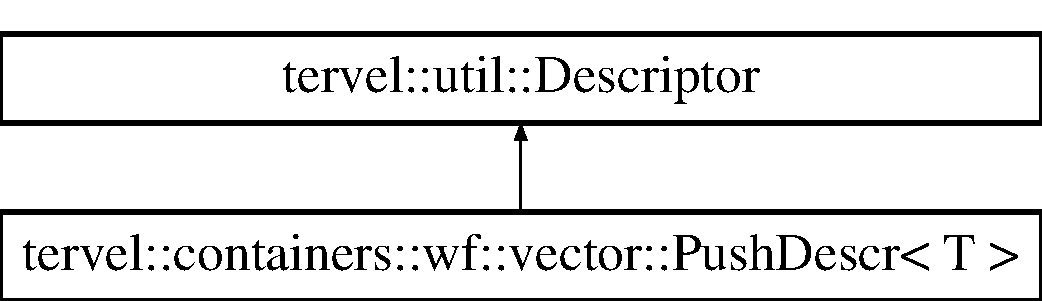
\includegraphics[height=2.000000cm]{classtervel_1_1containers_1_1wf_1_1vector_1_1_push_descr}
\end{center}
\end{figure}
\subsection*{Public Member Functions}
\begin{DoxyCompactItemize}
\item 
\hyperlink{classtervel_1_1containers_1_1wf_1_1vector_1_1_push_descr_af0089991c6b5ea3d30cac7a62129a553}{Push\+Descr} (T val, Vector$<$ T $>$ $\ast$vec)
\item 
void \hyperlink{classtervel_1_1containers_1_1wf_1_1vector_1_1_push_descr_a89ea642ab6bbe2f85027c20df8059308}{set\+\_\+prev\+\_\+spot} (std\+::atomic$<$ T $>$ $\ast$prev\+\_\+spot)
\item 
bool \hyperlink{classtervel_1_1containers_1_1wf_1_1vector_1_1_push_descr_a81fb90d94cb35aec8424b047011b31e3}{in\+\_\+progress} ()
\item 
bool \hyperlink{classtervel_1_1containers_1_1wf_1_1vector_1_1_push_descr_a8af9a44dc44815a8f844c47b4e7fde1f}{result} ()
\item 
bool \hyperlink{classtervel_1_1containers_1_1wf_1_1vector_1_1_push_descr_a618ee51ed91820baabce55f6f77bbf45}{success} ()
\item 
bool \hyperlink{classtervel_1_1containers_1_1wf_1_1vector_1_1_push_descr_aa136be2653a1d233e34016da44f13685}{fail} ()
\item 
void $\ast$ \hyperlink{classtervel_1_1containers_1_1wf_1_1vector_1_1_push_descr_ada1424d353cb887e5f6380f08d0e926a}{get\+\_\+logical\+\_\+value} ()
\begin{DoxyCompactList}\small\item\em This method is implemented by each sub class. \end{DoxyCompactList}\item 
void $\ast$ \hyperlink{classtervel_1_1containers_1_1wf_1_1vector_1_1_push_descr_aa8d94d395ac24a37566dfdde8616ff53}{complete} (void $\ast$value, std\+::atomic$<$ void $\ast$ $>$ $\ast$address)
\begin{DoxyCompactList}\small\item\em This method is implemented by each sub class and must guarantee that upon return that the descriptor no longer exists at the address it was placed. \end{DoxyCompactList}\item 
void \hyperlink{classtervel_1_1containers_1_1wf_1_1vector_1_1_push_descr_aecb481cfbf8b2f5d2a0dc603913bb237}{set\+\_\+control\+\_\+word} ()
\end{DoxyCompactItemize}
\subsection*{Private Attributes}
\begin{DoxyCompactItemize}
\item 
T \hyperlink{classtervel_1_1containers_1_1wf_1_1vector_1_1_push_descr_af9bcca18a4b5fd5cb92787655322bb32}{val\+\_\+}
\item 
Vector$<$ T $>$ $\ast$ \hyperlink{classtervel_1_1containers_1_1wf_1_1vector_1_1_push_descr_a4435889c7578aac40dd4355523b52238}{vec\+\_\+}
\item 
std\+::atomic$<$ T $>$ $\ast$ \hyperlink{classtervel_1_1containers_1_1wf_1_1vector_1_1_push_descr_a7ce9de884957d0e200233e71e59f417f}{prev\+\_\+spot\+\_\+} \{nullptr\}
\item 
std\+::atomic$<$ uint64\+\_\+t $>$ \hyperlink{classtervel_1_1containers_1_1wf_1_1vector_1_1_push_descr_a9aceab6795bc84efed74cad6d537e5e9}{success\+\_\+} \{0\}
\end{DoxyCompactItemize}


\subsection{Constructor \& Destructor Documentation}
\hypertarget{classtervel_1_1containers_1_1wf_1_1vector_1_1_push_descr_af0089991c6b5ea3d30cac7a62129a553}{}\index{tervel\+::containers\+::wf\+::vector\+::\+Push\+Descr@{tervel\+::containers\+::wf\+::vector\+::\+Push\+Descr}!Push\+Descr@{Push\+Descr}}
\index{Push\+Descr@{Push\+Descr}!tervel\+::containers\+::wf\+::vector\+::\+Push\+Descr@{tervel\+::containers\+::wf\+::vector\+::\+Push\+Descr}}
\subsubsection[{Push\+Descr(\+T val, Vector$<$ T $>$ $\ast$vec)}]{\setlength{\rightskip}{0pt plus 5cm}template$<$typename T$>$ {\bf tervel\+::containers\+::wf\+::vector\+::\+Push\+Descr}$<$ T $>$\+::{\bf Push\+Descr} (
\begin{DoxyParamCaption}
\item[{T}]{val, }
\item[{Vector$<$ T $>$ $\ast$}]{vec}
\end{DoxyParamCaption}
)\hspace{0.3cm}{\ttfamily [inline]}, {\ttfamily [explicit]}}\label{classtervel_1_1containers_1_1wf_1_1vector_1_1_push_descr_af0089991c6b5ea3d30cac7a62129a553}


\subsection{Member Function Documentation}
\hypertarget{classtervel_1_1containers_1_1wf_1_1vector_1_1_push_descr_aa8d94d395ac24a37566dfdde8616ff53}{}\index{tervel\+::containers\+::wf\+::vector\+::\+Push\+Descr@{tervel\+::containers\+::wf\+::vector\+::\+Push\+Descr}!complete@{complete}}
\index{complete@{complete}!tervel\+::containers\+::wf\+::vector\+::\+Push\+Descr@{tervel\+::containers\+::wf\+::vector\+::\+Push\+Descr}}
\subsubsection[{complete(void $\ast$value, std\+::atomic$<$ void $\ast$ $>$ $\ast$address)}]{\setlength{\rightskip}{0pt plus 5cm}template$<$typename T$>$ void$\ast$ {\bf tervel\+::containers\+::wf\+::vector\+::\+Push\+Descr}$<$ T $>$\+::complete (
\begin{DoxyParamCaption}
\item[{void $\ast$}]{current, }
\item[{std\+::atomic$<$ void $\ast$ $>$ $\ast$}]{address}
\end{DoxyParamCaption}
)\hspace{0.3cm}{\ttfamily [inline]}, {\ttfamily [virtual]}}\label{classtervel_1_1containers_1_1wf_1_1vector_1_1_push_descr_aa8d94d395ac24a37566dfdde8616ff53}


This method is implemented by each sub class and must guarantee that upon return that the descriptor no longer exists at the address it was placed. 


\begin{DoxyParams}{Parameters}
{\em current} & the reference to this object as it is at the address, \\
\hline
{\em address} & the location this object was read from \\
\hline
\end{DoxyParams}


Implements \hyperlink{classtervel_1_1util_1_1_descriptor_a4303b2a08e3ab67de5533cfb20db87c9}{tervel\+::util\+::\+Descriptor}.

\hypertarget{classtervel_1_1containers_1_1wf_1_1vector_1_1_push_descr_aa136be2653a1d233e34016da44f13685}{}\index{tervel\+::containers\+::wf\+::vector\+::\+Push\+Descr@{tervel\+::containers\+::wf\+::vector\+::\+Push\+Descr}!fail@{fail}}
\index{fail@{fail}!tervel\+::containers\+::wf\+::vector\+::\+Push\+Descr@{tervel\+::containers\+::wf\+::vector\+::\+Push\+Descr}}
\subsubsection[{fail()}]{\setlength{\rightskip}{0pt plus 5cm}template$<$typename T$>$ bool {\bf tervel\+::containers\+::wf\+::vector\+::\+Push\+Descr}$<$ T $>$\+::fail (
\begin{DoxyParamCaption}
{}
\end{DoxyParamCaption}
)\hspace{0.3cm}{\ttfamily [inline]}}\label{classtervel_1_1containers_1_1wf_1_1vector_1_1_push_descr_aa136be2653a1d233e34016da44f13685}
\hypertarget{classtervel_1_1containers_1_1wf_1_1vector_1_1_push_descr_ada1424d353cb887e5f6380f08d0e926a}{}\index{tervel\+::containers\+::wf\+::vector\+::\+Push\+Descr@{tervel\+::containers\+::wf\+::vector\+::\+Push\+Descr}!get\+\_\+logical\+\_\+value@{get\+\_\+logical\+\_\+value}}
\index{get\+\_\+logical\+\_\+value@{get\+\_\+logical\+\_\+value}!tervel\+::containers\+::wf\+::vector\+::\+Push\+Descr@{tervel\+::containers\+::wf\+::vector\+::\+Push\+Descr}}
\subsubsection[{get\+\_\+logical\+\_\+value()}]{\setlength{\rightskip}{0pt plus 5cm}template$<$typename T$>$ void$\ast$ {\bf tervel\+::containers\+::wf\+::vector\+::\+Push\+Descr}$<$ T $>$\+::get\+\_\+logical\+\_\+value (
\begin{DoxyParamCaption}
{}
\end{DoxyParamCaption}
)\hspace{0.3cm}{\ttfamily [inline]}, {\ttfamily [virtual]}}\label{classtervel_1_1containers_1_1wf_1_1vector_1_1_push_descr_ada1424d353cb887e5f6380f08d0e926a}


This method is implemented by each sub class. 

It returns the logical value of the past address. If the associated operation is still in progress then it will generally return the value that was replaced by this descriptor. Otherwise it will generally return the result of the operation for the specified address.

It can only be called from the static function which protects the object from being reused during the function. 

Implements \hyperlink{classtervel_1_1util_1_1_descriptor_a5b443eeb6acf1207f27a6d06c39d4ad4}{tervel\+::util\+::\+Descriptor}.

\hypertarget{classtervel_1_1containers_1_1wf_1_1vector_1_1_push_descr_a81fb90d94cb35aec8424b047011b31e3}{}\index{tervel\+::containers\+::wf\+::vector\+::\+Push\+Descr@{tervel\+::containers\+::wf\+::vector\+::\+Push\+Descr}!in\+\_\+progress@{in\+\_\+progress}}
\index{in\+\_\+progress@{in\+\_\+progress}!tervel\+::containers\+::wf\+::vector\+::\+Push\+Descr@{tervel\+::containers\+::wf\+::vector\+::\+Push\+Descr}}
\subsubsection[{in\+\_\+progress()}]{\setlength{\rightskip}{0pt plus 5cm}template$<$typename T$>$ bool {\bf tervel\+::containers\+::wf\+::vector\+::\+Push\+Descr}$<$ T $>$\+::in\+\_\+progress (
\begin{DoxyParamCaption}
{}
\end{DoxyParamCaption}
)\hspace{0.3cm}{\ttfamily [inline]}}\label{classtervel_1_1containers_1_1wf_1_1vector_1_1_push_descr_a81fb90d94cb35aec8424b047011b31e3}
\hypertarget{classtervel_1_1containers_1_1wf_1_1vector_1_1_push_descr_a8af9a44dc44815a8f844c47b4e7fde1f}{}\index{tervel\+::containers\+::wf\+::vector\+::\+Push\+Descr@{tervel\+::containers\+::wf\+::vector\+::\+Push\+Descr}!result@{result}}
\index{result@{result}!tervel\+::containers\+::wf\+::vector\+::\+Push\+Descr@{tervel\+::containers\+::wf\+::vector\+::\+Push\+Descr}}
\subsubsection[{result()}]{\setlength{\rightskip}{0pt plus 5cm}template$<$typename T$>$ bool {\bf tervel\+::containers\+::wf\+::vector\+::\+Push\+Descr}$<$ T $>$\+::result (
\begin{DoxyParamCaption}
{}
\end{DoxyParamCaption}
)\hspace{0.3cm}{\ttfamily [inline]}}\label{classtervel_1_1containers_1_1wf_1_1vector_1_1_push_descr_a8af9a44dc44815a8f844c47b4e7fde1f}
\hypertarget{classtervel_1_1containers_1_1wf_1_1vector_1_1_push_descr_aecb481cfbf8b2f5d2a0dc603913bb237}{}\index{tervel\+::containers\+::wf\+::vector\+::\+Push\+Descr@{tervel\+::containers\+::wf\+::vector\+::\+Push\+Descr}!set\+\_\+control\+\_\+word@{set\+\_\+control\+\_\+word}}
\index{set\+\_\+control\+\_\+word@{set\+\_\+control\+\_\+word}!tervel\+::containers\+::wf\+::vector\+::\+Push\+Descr@{tervel\+::containers\+::wf\+::vector\+::\+Push\+Descr}}
\subsubsection[{set\+\_\+control\+\_\+word()}]{\setlength{\rightskip}{0pt plus 5cm}template$<$typename T$>$ void {\bf tervel\+::containers\+::wf\+::vector\+::\+Push\+Descr}$<$ T $>$\+::set\+\_\+control\+\_\+word (
\begin{DoxyParamCaption}
{}
\end{DoxyParamCaption}
)\hspace{0.3cm}{\ttfamily [inline]}}\label{classtervel_1_1containers_1_1wf_1_1vector_1_1_push_descr_aecb481cfbf8b2f5d2a0dc603913bb237}
\hypertarget{classtervel_1_1containers_1_1wf_1_1vector_1_1_push_descr_a89ea642ab6bbe2f85027c20df8059308}{}\index{tervel\+::containers\+::wf\+::vector\+::\+Push\+Descr@{tervel\+::containers\+::wf\+::vector\+::\+Push\+Descr}!set\+\_\+prev\+\_\+spot@{set\+\_\+prev\+\_\+spot}}
\index{set\+\_\+prev\+\_\+spot@{set\+\_\+prev\+\_\+spot}!tervel\+::containers\+::wf\+::vector\+::\+Push\+Descr@{tervel\+::containers\+::wf\+::vector\+::\+Push\+Descr}}
\subsubsection[{set\+\_\+prev\+\_\+spot(std\+::atomic$<$ T $>$ $\ast$prev\+\_\+spot)}]{\setlength{\rightskip}{0pt plus 5cm}template$<$typename T$>$ void {\bf tervel\+::containers\+::wf\+::vector\+::\+Push\+Descr}$<$ T $>$\+::set\+\_\+prev\+\_\+spot (
\begin{DoxyParamCaption}
\item[{std\+::atomic$<$ T $>$ $\ast$}]{prev\+\_\+spot}
\end{DoxyParamCaption}
)\hspace{0.3cm}{\ttfamily [inline]}}\label{classtervel_1_1containers_1_1wf_1_1vector_1_1_push_descr_a89ea642ab6bbe2f85027c20df8059308}
\hypertarget{classtervel_1_1containers_1_1wf_1_1vector_1_1_push_descr_a618ee51ed91820baabce55f6f77bbf45}{}\index{tervel\+::containers\+::wf\+::vector\+::\+Push\+Descr@{tervel\+::containers\+::wf\+::vector\+::\+Push\+Descr}!success@{success}}
\index{success@{success}!tervel\+::containers\+::wf\+::vector\+::\+Push\+Descr@{tervel\+::containers\+::wf\+::vector\+::\+Push\+Descr}}
\subsubsection[{success()}]{\setlength{\rightskip}{0pt plus 5cm}template$<$typename T$>$ bool {\bf tervel\+::containers\+::wf\+::vector\+::\+Push\+Descr}$<$ T $>$\+::success (
\begin{DoxyParamCaption}
{}
\end{DoxyParamCaption}
)\hspace{0.3cm}{\ttfamily [inline]}}\label{classtervel_1_1containers_1_1wf_1_1vector_1_1_push_descr_a618ee51ed91820baabce55f6f77bbf45}


\subsection{Member Data Documentation}
\hypertarget{classtervel_1_1containers_1_1wf_1_1vector_1_1_push_descr_a7ce9de884957d0e200233e71e59f417f}{}\index{tervel\+::containers\+::wf\+::vector\+::\+Push\+Descr@{tervel\+::containers\+::wf\+::vector\+::\+Push\+Descr}!prev\+\_\+spot\+\_\+@{prev\+\_\+spot\+\_\+}}
\index{prev\+\_\+spot\+\_\+@{prev\+\_\+spot\+\_\+}!tervel\+::containers\+::wf\+::vector\+::\+Push\+Descr@{tervel\+::containers\+::wf\+::vector\+::\+Push\+Descr}}
\subsubsection[{prev\+\_\+spot\+\_\+}]{\setlength{\rightskip}{0pt plus 5cm}template$<$typename T$>$ std\+::atomic$<$T$>$$\ast$ {\bf tervel\+::containers\+::wf\+::vector\+::\+Push\+Descr}$<$ T $>$\+::prev\+\_\+spot\+\_\+ \{nullptr\}\hspace{0.3cm}{\ttfamily [private]}}\label{classtervel_1_1containers_1_1wf_1_1vector_1_1_push_descr_a7ce9de884957d0e200233e71e59f417f}
\hypertarget{classtervel_1_1containers_1_1wf_1_1vector_1_1_push_descr_a9aceab6795bc84efed74cad6d537e5e9}{}\index{tervel\+::containers\+::wf\+::vector\+::\+Push\+Descr@{tervel\+::containers\+::wf\+::vector\+::\+Push\+Descr}!success\+\_\+@{success\+\_\+}}
\index{success\+\_\+@{success\+\_\+}!tervel\+::containers\+::wf\+::vector\+::\+Push\+Descr@{tervel\+::containers\+::wf\+::vector\+::\+Push\+Descr}}
\subsubsection[{success\+\_\+}]{\setlength{\rightskip}{0pt plus 5cm}template$<$typename T$>$ std\+::atomic$<$uint64\+\_\+t$>$ {\bf tervel\+::containers\+::wf\+::vector\+::\+Push\+Descr}$<$ T $>$\+::success\+\_\+ \{0\}\hspace{0.3cm}{\ttfamily [private]}}\label{classtervel_1_1containers_1_1wf_1_1vector_1_1_push_descr_a9aceab6795bc84efed74cad6d537e5e9}
\hypertarget{classtervel_1_1containers_1_1wf_1_1vector_1_1_push_descr_af9bcca18a4b5fd5cb92787655322bb32}{}\index{tervel\+::containers\+::wf\+::vector\+::\+Push\+Descr@{tervel\+::containers\+::wf\+::vector\+::\+Push\+Descr}!val\+\_\+@{val\+\_\+}}
\index{val\+\_\+@{val\+\_\+}!tervel\+::containers\+::wf\+::vector\+::\+Push\+Descr@{tervel\+::containers\+::wf\+::vector\+::\+Push\+Descr}}
\subsubsection[{val\+\_\+}]{\setlength{\rightskip}{0pt plus 5cm}template$<$typename T$>$ T {\bf tervel\+::containers\+::wf\+::vector\+::\+Push\+Descr}$<$ T $>$\+::val\+\_\+\hspace{0.3cm}{\ttfamily [private]}}\label{classtervel_1_1containers_1_1wf_1_1vector_1_1_push_descr_af9bcca18a4b5fd5cb92787655322bb32}
\hypertarget{classtervel_1_1containers_1_1wf_1_1vector_1_1_push_descr_a4435889c7578aac40dd4355523b52238}{}\index{tervel\+::containers\+::wf\+::vector\+::\+Push\+Descr@{tervel\+::containers\+::wf\+::vector\+::\+Push\+Descr}!vec\+\_\+@{vec\+\_\+}}
\index{vec\+\_\+@{vec\+\_\+}!tervel\+::containers\+::wf\+::vector\+::\+Push\+Descr@{tervel\+::containers\+::wf\+::vector\+::\+Push\+Descr}}
\subsubsection[{vec\+\_\+}]{\setlength{\rightskip}{0pt plus 5cm}template$<$typename T$>$ Vector$<$T$>$$\ast$ {\bf tervel\+::containers\+::wf\+::vector\+::\+Push\+Descr}$<$ T $>$\+::vec\+\_\+\hspace{0.3cm}{\ttfamily [private]}}\label{classtervel_1_1containers_1_1wf_1_1vector_1_1_push_descr_a4435889c7578aac40dd4355523b52238}


The documentation for this class was generated from the following file\+:\begin{DoxyCompactItemize}
\item 
tervel/containers/wf/vector/\hyperlink{pushback__op_8h}{pushback\+\_\+op.\+h}\end{DoxyCompactItemize}

\hypertarget{class_push_helper}{}\section{Push\+Helper Class Reference}
\label{class_push_helper}\index{Push\+Helper@{Push\+Helper}}


{\ttfamily \#include $<$push\+\_\+helper.\+h$>$}

Inheritance diagram for Push\+Helper\+:\begin{figure}[H]
\begin{center}
\leavevmode
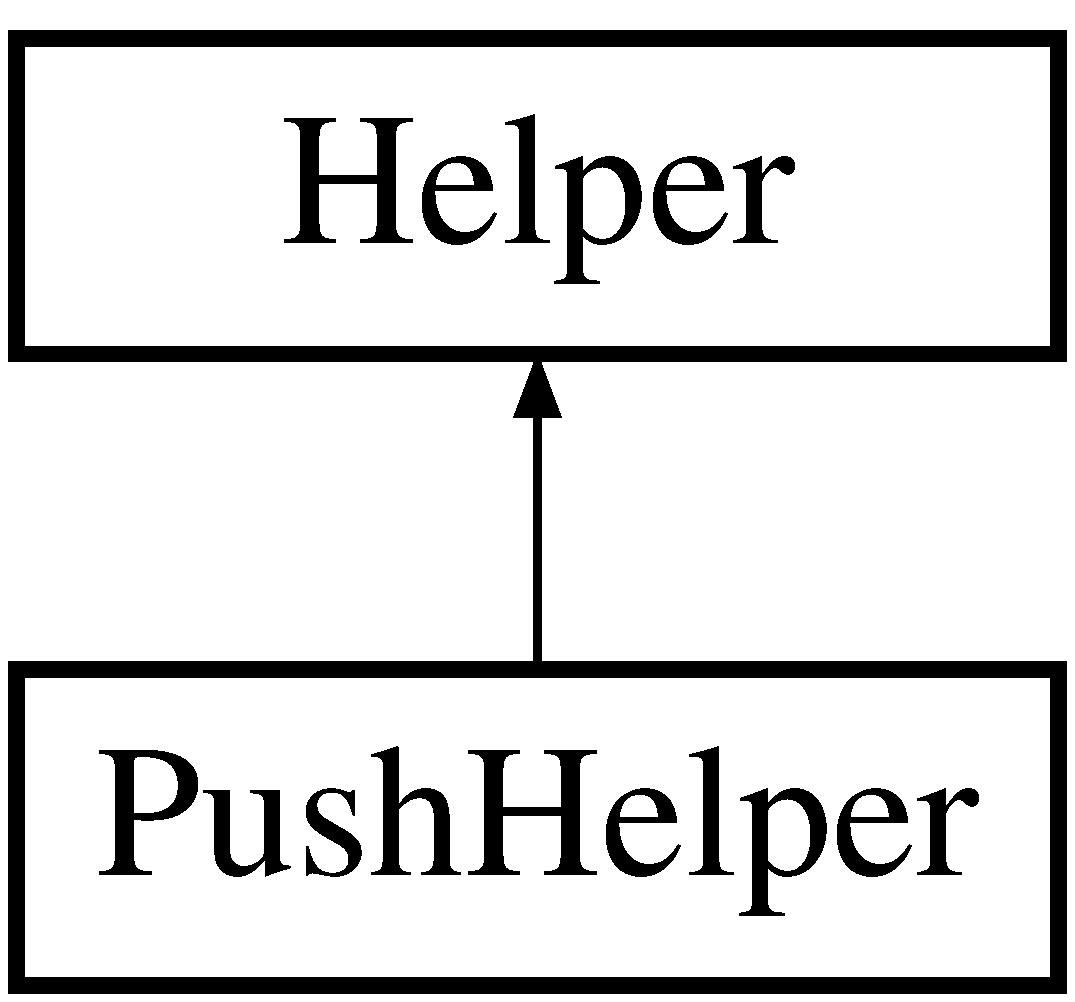
\includegraphics[height=2.000000cm]{class_push_helper}
\end{center}
\end{figure}
\subsection*{Public Member Functions}
\begin{DoxyCompactItemize}
\item 
void \hyperlink{class_push_helper_af0f2b3d32c4fa045423c0c33338fda6d}{init} (void $\ast$v, \hyperlink{class_push_op}{Push\+Op} $\ast$op)
\item 
\hyperlink{class_push_helper_a280f399f92564f84624c8044a7068fcf}{Push\+Helper} (void $\ast$v)
\item 
\hyperlink{class_push_helper_af0ae04521864c1ae2d3fa09e85d97fc6}{Push\+Helper} (void $\ast$v, \hyperlink{class_push_op}{Push\+Op} $\ast$op)
\item 
bool \hyperlink{class_push_helper_ad7439a580cc3979f4a8d024209f02a48}{complete} (W\+F\+Vector $\ast$vec, int \hyperlink{class_push_helper_afc30e140af18bc227c92363abeb504a1}{pos})
\item 
bool \hyperlink{class_push_helper_ad3a73efd37ac6b130da9892ce17a15f9}{try\+Free} ()
\item 
bool \hyperlink{class_push_helper_a3a766549de39a978203ec9e24d0adcce}{watch} (void $\ast$p, Array\+Element $\ast$a)
\item 
void \hyperlink{class_push_helper_ae5261cf5cc0aec9f9ea0e38bef6dec92}{unwatch} ()
\item 
bool \hyperlink{class_push_helper_aae1e891a2cde3c4d718bf02be0369a46}{is\+Watched} ()
\item 
void $\ast$ \hyperlink{class_push_helper_a3711a9e4be2b548b89f0c945907ceed0}{read\+Through} ()
\end{DoxyCompactItemize}
\subsection*{Public Attributes}
\begin{DoxyCompactItemize}
\item 
void $\ast$ \hyperlink{class_push_helper_af930dbddbf4d0ea5d0cb723d0dce7790}{value}
\item 
std\+::atomic$<$ long $>$ \hyperlink{class_push_helper_afc30e140af18bc227c92363abeb504a1}{pos}
\item 
\hyperlink{class_push_op}{Push\+Op} $\ast$ \hyperlink{class_push_helper_ada3667bd8ed54f5a7d2b0f89bdc08695}{control\+Op}
\end{DoxyCompactItemize}


\subsection{Constructor \& Destructor Documentation}
\hypertarget{class_push_helper_a280f399f92564f84624c8044a7068fcf}{}\index{Push\+Helper@{Push\+Helper}!Push\+Helper@{Push\+Helper}}
\index{Push\+Helper@{Push\+Helper}!Push\+Helper@{Push\+Helper}}
\subsubsection[{Push\+Helper(void $\ast$v)}]{\setlength{\rightskip}{0pt plus 5cm}Push\+Helper\+::\+Push\+Helper (
\begin{DoxyParamCaption}
\item[{void $\ast$}]{v}
\end{DoxyParamCaption}
)\hspace{0.3cm}{\ttfamily [inline]}}\label{class_push_helper_a280f399f92564f84624c8044a7068fcf}
\hypertarget{class_push_helper_af0ae04521864c1ae2d3fa09e85d97fc6}{}\index{Push\+Helper@{Push\+Helper}!Push\+Helper@{Push\+Helper}}
\index{Push\+Helper@{Push\+Helper}!Push\+Helper@{Push\+Helper}}
\subsubsection[{Push\+Helper(void $\ast$v, Push\+Op $\ast$op)}]{\setlength{\rightskip}{0pt plus 5cm}Push\+Helper\+::\+Push\+Helper (
\begin{DoxyParamCaption}
\item[{void $\ast$}]{v, }
\item[{{\bf Push\+Op} $\ast$}]{op}
\end{DoxyParamCaption}
)\hspace{0.3cm}{\ttfamily [inline]}}\label{class_push_helper_af0ae04521864c1ae2d3fa09e85d97fc6}


\subsection{Member Function Documentation}
\hypertarget{class_push_helper_ad7439a580cc3979f4a8d024209f02a48}{}\index{Push\+Helper@{Push\+Helper}!complete@{complete}}
\index{complete@{complete}!Push\+Helper@{Push\+Helper}}
\subsubsection[{complete(\+W\+F\+Vector $\ast$vec, int pos)}]{\setlength{\rightskip}{0pt plus 5cm}bool Push\+Helper\+::complete (
\begin{DoxyParamCaption}
\item[{W\+F\+Vector $\ast$}]{vec, }
\item[{int}]{pos}
\end{DoxyParamCaption}
)}\label{class_push_helper_ad7439a580cc3979f4a8d024209f02a48}
\hypertarget{class_push_helper_af0f2b3d32c4fa045423c0c33338fda6d}{}\index{Push\+Helper@{Push\+Helper}!init@{init}}
\index{init@{init}!Push\+Helper@{Push\+Helper}}
\subsubsection[{init(void $\ast$v, Push\+Op $\ast$op)}]{\setlength{\rightskip}{0pt plus 5cm}void Push\+Helper\+::init (
\begin{DoxyParamCaption}
\item[{void $\ast$}]{v, }
\item[{{\bf Push\+Op} $\ast$}]{op}
\end{DoxyParamCaption}
)\hspace{0.3cm}{\ttfamily [inline]}}\label{class_push_helper_af0f2b3d32c4fa045423c0c33338fda6d}
\hypertarget{class_push_helper_aae1e891a2cde3c4d718bf02be0369a46}{}\index{Push\+Helper@{Push\+Helper}!is\+Watched@{is\+Watched}}
\index{is\+Watched@{is\+Watched}!Push\+Helper@{Push\+Helper}}
\subsubsection[{is\+Watched()}]{\setlength{\rightskip}{0pt plus 5cm}bool Push\+Helper\+::is\+Watched (
\begin{DoxyParamCaption}
{}
\end{DoxyParamCaption}
)\hspace{0.3cm}{\ttfamily [inline]}}\label{class_push_helper_aae1e891a2cde3c4d718bf02be0369a46}
\hypertarget{class_push_helper_a3711a9e4be2b548b89f0c945907ceed0}{}\index{Push\+Helper@{Push\+Helper}!read\+Through@{read\+Through}}
\index{read\+Through@{read\+Through}!Push\+Helper@{Push\+Helper}}
\subsubsection[{read\+Through()}]{\setlength{\rightskip}{0pt plus 5cm}void$\ast$ Push\+Helper\+::read\+Through (
\begin{DoxyParamCaption}
{}
\end{DoxyParamCaption}
)\hspace{0.3cm}{\ttfamily [inline]}}\label{class_push_helper_a3711a9e4be2b548b89f0c945907ceed0}
\hypertarget{class_push_helper_ad3a73efd37ac6b130da9892ce17a15f9}{}\index{Push\+Helper@{Push\+Helper}!try\+Free@{try\+Free}}
\index{try\+Free@{try\+Free}!Push\+Helper@{Push\+Helper}}
\subsubsection[{try\+Free()}]{\setlength{\rightskip}{0pt plus 5cm}bool Push\+Helper\+::try\+Free (
\begin{DoxyParamCaption}
{}
\end{DoxyParamCaption}
)}\label{class_push_helper_ad3a73efd37ac6b130da9892ce17a15f9}
\hypertarget{class_push_helper_ae5261cf5cc0aec9f9ea0e38bef6dec92}{}\index{Push\+Helper@{Push\+Helper}!unwatch@{unwatch}}
\index{unwatch@{unwatch}!Push\+Helper@{Push\+Helper}}
\subsubsection[{unwatch()}]{\setlength{\rightskip}{0pt plus 5cm}void Push\+Helper\+::unwatch (
\begin{DoxyParamCaption}
{}
\end{DoxyParamCaption}
)\hspace{0.3cm}{\ttfamily [inline]}}\label{class_push_helper_ae5261cf5cc0aec9f9ea0e38bef6dec92}
\hypertarget{class_push_helper_a3a766549de39a978203ec9e24d0adcce}{}\index{Push\+Helper@{Push\+Helper}!watch@{watch}}
\index{watch@{watch}!Push\+Helper@{Push\+Helper}}
\subsubsection[{watch(void $\ast$p, Array\+Element $\ast$a)}]{\setlength{\rightskip}{0pt plus 5cm}bool Push\+Helper\+::watch (
\begin{DoxyParamCaption}
\item[{void $\ast$}]{p, }
\item[{Array\+Element $\ast$}]{a}
\end{DoxyParamCaption}
)\hspace{0.3cm}{\ttfamily [inline]}}\label{class_push_helper_a3a766549de39a978203ec9e24d0adcce}


\subsection{Member Data Documentation}
\hypertarget{class_push_helper_ada3667bd8ed54f5a7d2b0f89bdc08695}{}\index{Push\+Helper@{Push\+Helper}!control\+Op@{control\+Op}}
\index{control\+Op@{control\+Op}!Push\+Helper@{Push\+Helper}}
\subsubsection[{control\+Op}]{\setlength{\rightskip}{0pt plus 5cm}{\bf Push\+Op}$\ast$ Push\+Helper\+::control\+Op}\label{class_push_helper_ada3667bd8ed54f5a7d2b0f89bdc08695}
\hypertarget{class_push_helper_afc30e140af18bc227c92363abeb504a1}{}\index{Push\+Helper@{Push\+Helper}!pos@{pos}}
\index{pos@{pos}!Push\+Helper@{Push\+Helper}}
\subsubsection[{pos}]{\setlength{\rightskip}{0pt plus 5cm}std\+::atomic$<$long$>$ Push\+Helper\+::pos}\label{class_push_helper_afc30e140af18bc227c92363abeb504a1}
\hypertarget{class_push_helper_af930dbddbf4d0ea5d0cb723d0dce7790}{}\index{Push\+Helper@{Push\+Helper}!value@{value}}
\index{value@{value}!Push\+Helper@{Push\+Helper}}
\subsubsection[{value}]{\setlength{\rightskip}{0pt plus 5cm}void$\ast$ Push\+Helper\+::value}\label{class_push_helper_af930dbddbf4d0ea5d0cb723d0dce7790}


The documentation for this class was generated from the following file\+:\begin{DoxyCompactItemize}
\item 
tervel/containers/wf/vector/old/\hyperlink{push__helper_8h}{push\+\_\+helper.\+h}\end{DoxyCompactItemize}

\hypertarget{class_push_op}{}\section{Push\+Op$<$ T $>$ Class Template Reference}
\label{class_push_op}\index{Push\+Op$<$ T $>$@{Push\+Op$<$ T $>$}}


{\ttfamily \#include $<$push\+\_\+op.\+h$>$}

Inheritance diagram for Push\+Op$<$ T $>$\+:\begin{figure}[H]
\begin{center}
\leavevmode
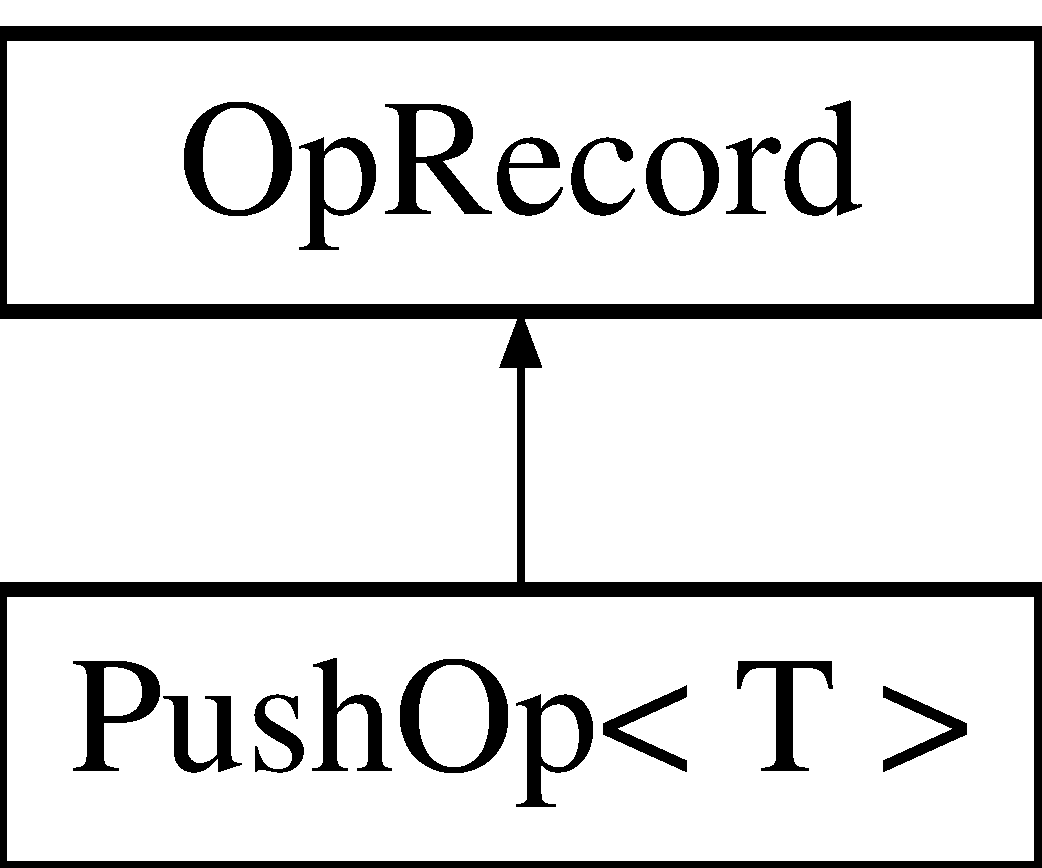
\includegraphics[height=2.000000cm]{class_push_op}
\end{center}
\end{figure}
\subsection*{Public Member Functions}
\begin{DoxyCompactItemize}
\item 
\hyperlink{class_push_op_afcac5a846e52a1f6b168dda598d3baa3}{Push\+Op} (Vector vector, T value)
\item 
size\+\_\+t \hyperlink{class_push_op_a97f81fb7d200909bdeb6e8346b8f485f}{begin} ()
\item 
void \hyperlink{class_push_op_a8a78c3baaa55f3b865910024c345176e}{execute} ()
\end{DoxyCompactItemize}
\subsection*{Public Attributes}
\begin{DoxyCompactItemize}
\item 
std\+::atomic$<$ \hyperlink{class_push_helper}{Push\+Helper}$<$ T $>$ $\ast$ $>$ \hyperlink{class_push_op_a1178c6780368c2f964386abc81f90298}{helper\+\_\+} \{nullptr\}
\item 
std\+::atomic$<$ size\+\_\+t $>$ \hyperlink{class_push_op_a0e4c04016077802998713feb9e5dc6fb}{pos\+\_\+} \{-\/1\}
\item 
const Vector vector\+\_\+ const T \hyperlink{class_push_op_af5df9efc25c3879d9178ccf9282de290}{value\+\_\+}
\end{DoxyCompactItemize}


\subsection{Constructor \& Destructor Documentation}
\hypertarget{class_push_op_afcac5a846e52a1f6b168dda598d3baa3}{}\index{Push\+Op@{Push\+Op}!Push\+Op@{Push\+Op}}
\index{Push\+Op@{Push\+Op}!Push\+Op@{Push\+Op}}
\subsubsection[{Push\+Op(\+Vector vector, T value)}]{\setlength{\rightskip}{0pt plus 5cm}template$<$class T $>$ {\bf Push\+Op}$<$ T $>$\+::{\bf Push\+Op} (
\begin{DoxyParamCaption}
\item[{Vector}]{vector, }
\item[{T}]{value}
\end{DoxyParamCaption}
)\hspace{0.3cm}{\ttfamily [inline]}}\label{class_push_op_afcac5a846e52a1f6b168dda598d3baa3}


\subsection{Member Function Documentation}
\hypertarget{class_push_op_a97f81fb7d200909bdeb6e8346b8f485f}{}\index{Push\+Op@{Push\+Op}!begin@{begin}}
\index{begin@{begin}!Push\+Op@{Push\+Op}}
\subsubsection[{begin()}]{\setlength{\rightskip}{0pt plus 5cm}template$<$class T $>$ size\+\_\+t {\bf Push\+Op}$<$ T $>$\+::begin (
\begin{DoxyParamCaption}
{}
\end{DoxyParamCaption}
)}\label{class_push_op_a97f81fb7d200909bdeb6e8346b8f485f}
\hypertarget{class_push_op_a8a78c3baaa55f3b865910024c345176e}{}\index{Push\+Op@{Push\+Op}!execute@{execute}}
\index{execute@{execute}!Push\+Op@{Push\+Op}}
\subsubsection[{execute()}]{\setlength{\rightskip}{0pt plus 5cm}template$<$class T $>$ void {\bf Push\+Op}$<$ T $>$\+::execute (
\begin{DoxyParamCaption}
{}
\end{DoxyParamCaption}
)}\label{class_push_op_a8a78c3baaa55f3b865910024c345176e}


\subsection{Member Data Documentation}
\hypertarget{class_push_op_a1178c6780368c2f964386abc81f90298}{}\index{Push\+Op@{Push\+Op}!helper\+\_\+@{helper\+\_\+}}
\index{helper\+\_\+@{helper\+\_\+}!Push\+Op@{Push\+Op}}
\subsubsection[{helper\+\_\+}]{\setlength{\rightskip}{0pt plus 5cm}template$<$class T $>$ std\+::atomic$<${\bf Push\+Helper}$<$T$>$ $\ast$$>$ {\bf Push\+Op}$<$ T $>$\+::helper\+\_\+ \{nullptr\}}\label{class_push_op_a1178c6780368c2f964386abc81f90298}
\hypertarget{class_push_op_a0e4c04016077802998713feb9e5dc6fb}{}\index{Push\+Op@{Push\+Op}!pos\+\_\+@{pos\+\_\+}}
\index{pos\+\_\+@{pos\+\_\+}!Push\+Op@{Push\+Op}}
\subsubsection[{pos\+\_\+}]{\setlength{\rightskip}{0pt plus 5cm}template$<$class T $>$ std\+::atomic$<$size\+\_\+t$>$ {\bf Push\+Op}$<$ T $>$\+::pos\+\_\+ \{-\/1\}}\label{class_push_op_a0e4c04016077802998713feb9e5dc6fb}
\hypertarget{class_push_op_af5df9efc25c3879d9178ccf9282de290}{}\index{Push\+Op@{Push\+Op}!value\+\_\+@{value\+\_\+}}
\index{value\+\_\+@{value\+\_\+}!Push\+Op@{Push\+Op}}
\subsubsection[{value\+\_\+}]{\setlength{\rightskip}{0pt plus 5cm}template$<$class T $>$ const Vector vector\+\_\+ const T {\bf Push\+Op}$<$ T $>$\+::value\+\_\+}\label{class_push_op_af5df9efc25c3879d9178ccf9282de290}


The documentation for this class was generated from the following file\+:\begin{DoxyCompactItemize}
\item 
tervel/containers/wf/vector/old/\hyperlink{push__op_8h}{push\+\_\+op.\+h}\end{DoxyCompactItemize}

\hypertarget{classtervel_1_1containers_1_1wf_1_1vector_1_1_push_op}{}\section{tervel\+:\+:containers\+:\+:wf\+:\+:vector\+:\+:Push\+Op$<$ T $>$ Class Template Reference}
\label{classtervel_1_1containers_1_1wf_1_1vector_1_1_push_op}\index{tervel\+::containers\+::wf\+::vector\+::\+Push\+Op$<$ T $>$@{tervel\+::containers\+::wf\+::vector\+::\+Push\+Op$<$ T $>$}}


{\ttfamily \#include $<$pushback\+\_\+op.\+h$>$}

Inheritance diagram for tervel\+:\+:containers\+:\+:wf\+:\+:vector\+:\+:Push\+Op$<$ T $>$\+:\begin{figure}[H]
\begin{center}
\leavevmode
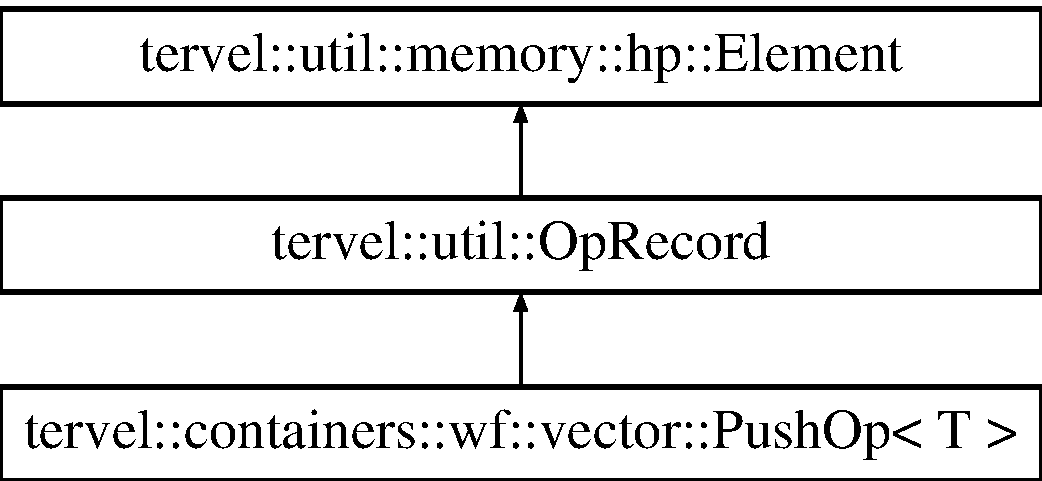
\includegraphics[height=3.000000cm]{classtervel_1_1containers_1_1wf_1_1vector_1_1_push_op}
\end{center}
\end{figure}
\subsection*{Public Member Functions}
\begin{DoxyCompactItemize}
\item 
\hyperlink{classtervel_1_1containers_1_1wf_1_1vector_1_1_push_op_a34175390fd8b79ed7f0cf9e00c0aacd6}{Push\+Op} (Vector$<$ T $>$ $\ast$vec, T val)
\item 
\hyperlink{classtervel_1_1containers_1_1wf_1_1vector_1_1_push_op_a9f4cfedad3558646b4ac15af5135b8ca}{$\sim$\+Push\+Op} ()
\item 
uint64\+\_\+t \hyperlink{classtervel_1_1containers_1_1wf_1_1vector_1_1_push_op_a6f55541df2382c5a269a5d88d8980952}{result} ()
\item 
void \hyperlink{classtervel_1_1containers_1_1wf_1_1vector_1_1_push_op_aca23a90c8ef1a6ac95a102def3b63d56}{help\+\_\+complete} ()
\begin{DoxyCompactList}\small\item\em Implementations of this function that upon its return the operation described in the Op\+Record has been completed. \end{DoxyCompactList}\item 
bool \hyperlink{classtervel_1_1containers_1_1wf_1_1vector_1_1_push_op_a3f3e9e0b7f1ea3c99ef17bb4dc8efc94}{is\+\_\+watched} ()
\end{DoxyCompactItemize}
\subsection*{Static Public Member Functions}
\begin{DoxyCompactItemize}
\item 
static size\+\_\+t \hyperlink{classtervel_1_1containers_1_1wf_1_1vector_1_1_push_op_adb5e668f536428dbda367da3dee6a94d}{execute} (Vector$<$ T $>$ $\ast$vec, T val)
\end{DoxyCompactItemize}
\subsection*{Private Attributes}
\begin{DoxyCompactItemize}
\item 
Vector$<$ T $>$ $\ast$ \hyperlink{classtervel_1_1containers_1_1wf_1_1vector_1_1_push_op_ace670d6d64e1f884f6213135d32d6dbe}{vec\+\_\+}
\item 
T \hyperlink{classtervel_1_1containers_1_1wf_1_1vector_1_1_push_op_a7e4e5a4d2436799e0b31bb82e0b4a0f6}{new\+\_\+val\+\_\+}
\item 
std\+::atomic$<$ \hyperlink{classtervel_1_1containers_1_1wf_1_1vector_1_1_push_op_helper}{Push\+Op\+Helper}$<$ T $>$ $\ast$ $>$ \hyperlink{classtervel_1_1containers_1_1wf_1_1vector_1_1_push_op_a285817a3099b8cda383eaf8f514d3496}{helper\+\_\+} \{nullptr\}
\end{DoxyCompactItemize}
\subsection*{Friends}
\begin{DoxyCompactItemize}
\item 
class \hyperlink{classtervel_1_1containers_1_1wf_1_1vector_1_1_push_op_a9620c687e3f69231ae07963424a2c308}{Push\+Op\+Helper$<$ T $>$}
\end{DoxyCompactItemize}


\subsection{Constructor \& Destructor Documentation}
\hypertarget{classtervel_1_1containers_1_1wf_1_1vector_1_1_push_op_a34175390fd8b79ed7f0cf9e00c0aacd6}{}\index{tervel\+::containers\+::wf\+::vector\+::\+Push\+Op@{tervel\+::containers\+::wf\+::vector\+::\+Push\+Op}!Push\+Op@{Push\+Op}}
\index{Push\+Op@{Push\+Op}!tervel\+::containers\+::wf\+::vector\+::\+Push\+Op@{tervel\+::containers\+::wf\+::vector\+::\+Push\+Op}}
\subsubsection[{Push\+Op(\+Vector$<$ T $>$ $\ast$vec, T val)}]{\setlength{\rightskip}{0pt plus 5cm}template$<$typename T$>$ {\bf tervel\+::containers\+::wf\+::vector\+::\+Push\+Op}$<$ T $>$\+::{\bf Push\+Op} (
\begin{DoxyParamCaption}
\item[{Vector$<$ T $>$ $\ast$}]{vec, }
\item[{T}]{val}
\end{DoxyParamCaption}
)\hspace{0.3cm}{\ttfamily [inline]}}\label{classtervel_1_1containers_1_1wf_1_1vector_1_1_push_op_a34175390fd8b79ed7f0cf9e00c0aacd6}
\hypertarget{classtervel_1_1containers_1_1wf_1_1vector_1_1_push_op_a9f4cfedad3558646b4ac15af5135b8ca}{}\index{tervel\+::containers\+::wf\+::vector\+::\+Push\+Op@{tervel\+::containers\+::wf\+::vector\+::\+Push\+Op}!````~Push\+Op@{$\sim$\+Push\+Op}}
\index{````~Push\+Op@{$\sim$\+Push\+Op}!tervel\+::containers\+::wf\+::vector\+::\+Push\+Op@{tervel\+::containers\+::wf\+::vector\+::\+Push\+Op}}
\subsubsection[{$\sim$\+Push\+Op()}]{\setlength{\rightskip}{0pt plus 5cm}template$<$typename T$>$ {\bf tervel\+::containers\+::wf\+::vector\+::\+Push\+Op}$<$ T $>$\+::$\sim${\bf Push\+Op} (
\begin{DoxyParamCaption}
{}
\end{DoxyParamCaption}
)\hspace{0.3cm}{\ttfamily [inline]}}\label{classtervel_1_1containers_1_1wf_1_1vector_1_1_push_op_a9f4cfedad3558646b4ac15af5135b8ca}


\subsection{Member Function Documentation}
\hypertarget{classtervel_1_1containers_1_1wf_1_1vector_1_1_push_op_adb5e668f536428dbda367da3dee6a94d}{}\index{tervel\+::containers\+::wf\+::vector\+::\+Push\+Op@{tervel\+::containers\+::wf\+::vector\+::\+Push\+Op}!execute@{execute}}
\index{execute@{execute}!tervel\+::containers\+::wf\+::vector\+::\+Push\+Op@{tervel\+::containers\+::wf\+::vector\+::\+Push\+Op}}
\subsubsection[{execute(\+Vector$<$ T $>$ $\ast$vec, T val)}]{\setlength{\rightskip}{0pt plus 5cm}template$<$typename T$>$ static size\+\_\+t {\bf tervel\+::containers\+::wf\+::vector\+::\+Push\+Op}$<$ T $>$\+::execute (
\begin{DoxyParamCaption}
\item[{Vector$<$ T $>$ $\ast$}]{vec, }
\item[{T}]{val}
\end{DoxyParamCaption}
)\hspace{0.3cm}{\ttfamily [inline]}, {\ttfamily [static]}}\label{classtervel_1_1containers_1_1wf_1_1vector_1_1_push_op_adb5e668f536428dbda367da3dee6a94d}
\hypertarget{classtervel_1_1containers_1_1wf_1_1vector_1_1_push_op_aca23a90c8ef1a6ac95a102def3b63d56}{}\index{tervel\+::containers\+::wf\+::vector\+::\+Push\+Op@{tervel\+::containers\+::wf\+::vector\+::\+Push\+Op}!help\+\_\+complete@{help\+\_\+complete}}
\index{help\+\_\+complete@{help\+\_\+complete}!tervel\+::containers\+::wf\+::vector\+::\+Push\+Op@{tervel\+::containers\+::wf\+::vector\+::\+Push\+Op}}
\subsubsection[{help\+\_\+complete()}]{\setlength{\rightskip}{0pt plus 5cm}template$<$typename T$>$ void {\bf tervel\+::containers\+::wf\+::vector\+::\+Push\+Op}$<$ T $>$\+::help\+\_\+complete (
\begin{DoxyParamCaption}
{}
\end{DoxyParamCaption}
)\hspace{0.3cm}{\ttfamily [inline]}, {\ttfamily [virtual]}}\label{classtervel_1_1containers_1_1wf_1_1vector_1_1_push_op_aca23a90c8ef1a6ac95a102def3b63d56}


Implementations of this function that upon its return the operation described in the Op\+Record has been completed. 

As such it must be thread-\/safe and the extending class must contain all the information necessary to complete the operation. 

Implements \hyperlink{classtervel_1_1util_1_1_op_record_aa75ab39688a8d4cceb6a1ef0409537c0}{tervel\+::util\+::\+Op\+Record}.

\hypertarget{classtervel_1_1containers_1_1wf_1_1vector_1_1_push_op_a3f3e9e0b7f1ea3c99ef17bb4dc8efc94}{}\index{tervel\+::containers\+::wf\+::vector\+::\+Push\+Op@{tervel\+::containers\+::wf\+::vector\+::\+Push\+Op}!is\+\_\+watched@{is\+\_\+watched}}
\index{is\+\_\+watched@{is\+\_\+watched}!tervel\+::containers\+::wf\+::vector\+::\+Push\+Op@{tervel\+::containers\+::wf\+::vector\+::\+Push\+Op}}
\subsubsection[{is\+\_\+watched()}]{\setlength{\rightskip}{0pt plus 5cm}template$<$typename T$>$ bool {\bf tervel\+::containers\+::wf\+::vector\+::\+Push\+Op}$<$ T $>$\+::is\+\_\+watched (
\begin{DoxyParamCaption}
{}
\end{DoxyParamCaption}
)\hspace{0.3cm}{\ttfamily [inline]}}\label{classtervel_1_1containers_1_1wf_1_1vector_1_1_push_op_a3f3e9e0b7f1ea3c99ef17bb4dc8efc94}
\hypertarget{classtervel_1_1containers_1_1wf_1_1vector_1_1_push_op_a6f55541df2382c5a269a5d88d8980952}{}\index{tervel\+::containers\+::wf\+::vector\+::\+Push\+Op@{tervel\+::containers\+::wf\+::vector\+::\+Push\+Op}!result@{result}}
\index{result@{result}!tervel\+::containers\+::wf\+::vector\+::\+Push\+Op@{tervel\+::containers\+::wf\+::vector\+::\+Push\+Op}}
\subsubsection[{result()}]{\setlength{\rightskip}{0pt plus 5cm}template$<$typename T$>$ uint64\+\_\+t {\bf tervel\+::containers\+::wf\+::vector\+::\+Push\+Op}$<$ T $>$\+::result (
\begin{DoxyParamCaption}
{}
\end{DoxyParamCaption}
)\hspace{0.3cm}{\ttfamily [inline]}}\label{classtervel_1_1containers_1_1wf_1_1vector_1_1_push_op_a6f55541df2382c5a269a5d88d8980952}


\subsection{Friends And Related Function Documentation}
\hypertarget{classtervel_1_1containers_1_1wf_1_1vector_1_1_push_op_a9620c687e3f69231ae07963424a2c308}{}\index{tervel\+::containers\+::wf\+::vector\+::\+Push\+Op@{tervel\+::containers\+::wf\+::vector\+::\+Push\+Op}!Push\+Op\+Helper$<$ T $>$@{Push\+Op\+Helper$<$ T $>$}}
\index{Push\+Op\+Helper$<$ T $>$@{Push\+Op\+Helper$<$ T $>$}!tervel\+::containers\+::wf\+::vector\+::\+Push\+Op@{tervel\+::containers\+::wf\+::vector\+::\+Push\+Op}}
\subsubsection[{Push\+Op\+Helper$<$ T $>$}]{\setlength{\rightskip}{0pt plus 5cm}template$<$typename T$>$ friend class {\bf Push\+Op\+Helper}$<$ T $>$\hspace{0.3cm}{\ttfamily [friend]}}\label{classtervel_1_1containers_1_1wf_1_1vector_1_1_push_op_a9620c687e3f69231ae07963424a2c308}


\subsection{Member Data Documentation}
\hypertarget{classtervel_1_1containers_1_1wf_1_1vector_1_1_push_op_a285817a3099b8cda383eaf8f514d3496}{}\index{tervel\+::containers\+::wf\+::vector\+::\+Push\+Op@{tervel\+::containers\+::wf\+::vector\+::\+Push\+Op}!helper\+\_\+@{helper\+\_\+}}
\index{helper\+\_\+@{helper\+\_\+}!tervel\+::containers\+::wf\+::vector\+::\+Push\+Op@{tervel\+::containers\+::wf\+::vector\+::\+Push\+Op}}
\subsubsection[{helper\+\_\+}]{\setlength{\rightskip}{0pt plus 5cm}template$<$typename T$>$ std\+::atomic$<${\bf Push\+Op\+Helper}$<$T$>$ $\ast$$>$ {\bf tervel\+::containers\+::wf\+::vector\+::\+Push\+Op}$<$ T $>$\+::helper\+\_\+ \{nullptr\}\hspace{0.3cm}{\ttfamily [private]}}\label{classtervel_1_1containers_1_1wf_1_1vector_1_1_push_op_a285817a3099b8cda383eaf8f514d3496}
\hypertarget{classtervel_1_1containers_1_1wf_1_1vector_1_1_push_op_a7e4e5a4d2436799e0b31bb82e0b4a0f6}{}\index{tervel\+::containers\+::wf\+::vector\+::\+Push\+Op@{tervel\+::containers\+::wf\+::vector\+::\+Push\+Op}!new\+\_\+val\+\_\+@{new\+\_\+val\+\_\+}}
\index{new\+\_\+val\+\_\+@{new\+\_\+val\+\_\+}!tervel\+::containers\+::wf\+::vector\+::\+Push\+Op@{tervel\+::containers\+::wf\+::vector\+::\+Push\+Op}}
\subsubsection[{new\+\_\+val\+\_\+}]{\setlength{\rightskip}{0pt plus 5cm}template$<$typename T$>$ T {\bf tervel\+::containers\+::wf\+::vector\+::\+Push\+Op}$<$ T $>$\+::new\+\_\+val\+\_\+\hspace{0.3cm}{\ttfamily [private]}}\label{classtervel_1_1containers_1_1wf_1_1vector_1_1_push_op_a7e4e5a4d2436799e0b31bb82e0b4a0f6}
\hypertarget{classtervel_1_1containers_1_1wf_1_1vector_1_1_push_op_ace670d6d64e1f884f6213135d32d6dbe}{}\index{tervel\+::containers\+::wf\+::vector\+::\+Push\+Op@{tervel\+::containers\+::wf\+::vector\+::\+Push\+Op}!vec\+\_\+@{vec\+\_\+}}
\index{vec\+\_\+@{vec\+\_\+}!tervel\+::containers\+::wf\+::vector\+::\+Push\+Op@{tervel\+::containers\+::wf\+::vector\+::\+Push\+Op}}
\subsubsection[{vec\+\_\+}]{\setlength{\rightskip}{0pt plus 5cm}template$<$typename T$>$ Vector$<$T$>$$\ast$ {\bf tervel\+::containers\+::wf\+::vector\+::\+Push\+Op}$<$ T $>$\+::vec\+\_\+\hspace{0.3cm}{\ttfamily [private]}}\label{classtervel_1_1containers_1_1wf_1_1vector_1_1_push_op_ace670d6d64e1f884f6213135d32d6dbe}


The documentation for this class was generated from the following file\+:\begin{DoxyCompactItemize}
\item 
tervel/containers/wf/vector/\hyperlink{pushback__op_8h}{pushback\+\_\+op.\+h}\end{DoxyCompactItemize}

\hypertarget{classtervel_1_1containers_1_1wf_1_1vector_1_1_push_op_helper}{}\section{tervel\+:\+:containers\+:\+:wf\+:\+:vector\+:\+:Push\+Op\+Helper$<$ T $>$ Class Template Reference}
\label{classtervel_1_1containers_1_1wf_1_1vector_1_1_push_op_helper}\index{tervel\+::containers\+::wf\+::vector\+::\+Push\+Op\+Helper$<$ T $>$@{tervel\+::containers\+::wf\+::vector\+::\+Push\+Op\+Helper$<$ T $>$}}


{\ttfamily \#include $<$pushback\+\_\+op.\+h$>$}

Inheritance diagram for tervel\+:\+:containers\+:\+:wf\+:\+:vector\+:\+:Push\+Op\+Helper$<$ T $>$\+:\begin{figure}[H]
\begin{center}
\leavevmode
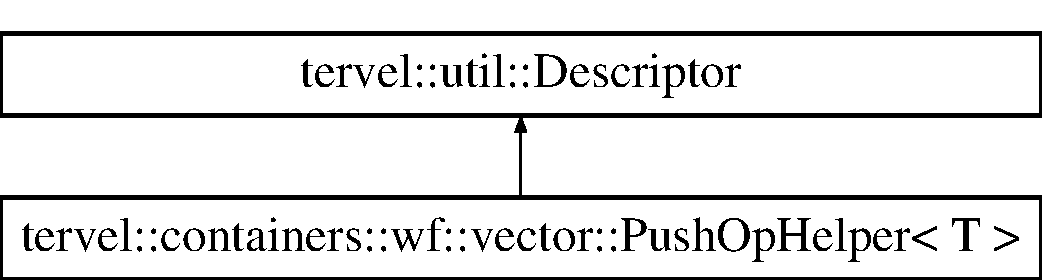
\includegraphics[height=2.000000cm]{classtervel_1_1containers_1_1wf_1_1vector_1_1_push_op_helper}
\end{center}
\end{figure}
\subsection*{Public Member Functions}
\begin{DoxyCompactItemize}
\item 
\hyperlink{classtervel_1_1containers_1_1wf_1_1vector_1_1_push_op_helper_acc95d398d2f1a4bd3c45c4298c725890}{Push\+Op\+Helper} (\hyperlink{classtervel_1_1containers_1_1wf_1_1vector_1_1_push_op}{Push\+Op}$<$ T $>$ $\ast$op)
\item 
void \hyperlink{classtervel_1_1containers_1_1wf_1_1vector_1_1_push_op_helper_a115505902a70a19edfaef728b52f4412}{set\+\_\+idx} (uint64\+\_\+t i)
\item 
uint64\+\_\+t \hyperlink{classtervel_1_1containers_1_1wf_1_1vector_1_1_push_op_helper_ad4d9ab60599e150df880aa38c47c45cd}{idx} ()
\item 
bool \hyperlink{classtervel_1_1containers_1_1wf_1_1vector_1_1_push_op_helper_a084d0f4f0f5142710a9fcafb982f21ec}{in\+\_\+progress} ()
\item 
bool \hyperlink{classtervel_1_1containers_1_1wf_1_1vector_1_1_push_op_helper_a010f036e1c51a25d5fcf152407b63e2b}{result} ()
\item 
bool \hyperlink{classtervel_1_1containers_1_1wf_1_1vector_1_1_push_op_helper_ac34386c36abb6e0ba4c8224661b7a931}{associate} ()
\item 
bool \hyperlink{classtervel_1_1containers_1_1wf_1_1vector_1_1_push_op_helper_a069caab9b05921b39a012ee4afde6eb7}{success} ()
\item 
bool \hyperlink{classtervel_1_1containers_1_1wf_1_1vector_1_1_push_op_helper_ae967c33c5e34bc9a9107043d0738fae2}{fail} ()
\item 
void $\ast$ \hyperlink{classtervel_1_1containers_1_1wf_1_1vector_1_1_push_op_helper_a8faede3c50015027a4738b5a626c1ea6}{complete} (void $\ast$value, std\+::atomic$<$ void $\ast$ $>$ $\ast$address)
\begin{DoxyCompactList}\small\item\em This method is implemented by each sub class and must guarantee that upon return that the descriptor no longer exists at the address it was placed. \end{DoxyCompactList}\item 
void $\ast$ \hyperlink{classtervel_1_1containers_1_1wf_1_1vector_1_1_push_op_helper_aa8ba2c9d99007ae04325294413601cff}{get\+\_\+logical\+\_\+value} ()
\begin{DoxyCompactList}\small\item\em This method is implemented by each sub class. \end{DoxyCompactList}\item 
bool \hyperlink{classtervel_1_1containers_1_1wf_1_1vector_1_1_push_op_helper_a26ce47d7b64eedcf1983508f5a60d5b7}{on\+\_\+watch} (std\+::atomic$<$ void $\ast$ $>$ $\ast$address, void $\ast$value)
\begin{DoxyCompactList}\small\item\em This method is optional to implement for each sub class. \end{DoxyCompactList}\end{DoxyCompactItemize}
\subsection*{Private Attributes}
\begin{DoxyCompactItemize}
\item 
\hyperlink{classtervel_1_1containers_1_1wf_1_1vector_1_1_push_op}{Push\+Op}$<$ T $>$ $\ast$ \hyperlink{classtervel_1_1containers_1_1wf_1_1vector_1_1_push_op_helper_ac6c7fb6c7872217ddfbf83d83b426ecd}{op\+\_\+}
\item 
uint64\+\_\+t \hyperlink{classtervel_1_1containers_1_1wf_1_1vector_1_1_push_op_helper_a8c2d10cc9b73cbc5ccabac7e12b9f325}{idx\+\_\+}
\item 
std\+::atomic$<$ uint64\+\_\+t $>$ \hyperlink{classtervel_1_1containers_1_1wf_1_1vector_1_1_push_op_helper_ade5d081b54d4b44fc773cfb2e09035e4}{success\+\_\+} \{0\}
\end{DoxyCompactItemize}


\subsection{Constructor \& Destructor Documentation}
\hypertarget{classtervel_1_1containers_1_1wf_1_1vector_1_1_push_op_helper_acc95d398d2f1a4bd3c45c4298c725890}{}\index{tervel\+::containers\+::wf\+::vector\+::\+Push\+Op\+Helper@{tervel\+::containers\+::wf\+::vector\+::\+Push\+Op\+Helper}!Push\+Op\+Helper@{Push\+Op\+Helper}}
\index{Push\+Op\+Helper@{Push\+Op\+Helper}!tervel\+::containers\+::wf\+::vector\+::\+Push\+Op\+Helper@{tervel\+::containers\+::wf\+::vector\+::\+Push\+Op\+Helper}}
\subsubsection[{Push\+Op\+Helper(\+Push\+Op$<$ T $>$ $\ast$op)}]{\setlength{\rightskip}{0pt plus 5cm}template$<$typename T$>$ {\bf tervel\+::containers\+::wf\+::vector\+::\+Push\+Op\+Helper}$<$ T $>$\+::{\bf Push\+Op\+Helper} (
\begin{DoxyParamCaption}
\item[{{\bf Push\+Op}$<$ T $>$ $\ast$}]{op}
\end{DoxyParamCaption}
)\hspace{0.3cm}{\ttfamily [inline]}, {\ttfamily [explicit]}}\label{classtervel_1_1containers_1_1wf_1_1vector_1_1_push_op_helper_acc95d398d2f1a4bd3c45c4298c725890}


\subsection{Member Function Documentation}
\hypertarget{classtervel_1_1containers_1_1wf_1_1vector_1_1_push_op_helper_ac34386c36abb6e0ba4c8224661b7a931}{}\index{tervel\+::containers\+::wf\+::vector\+::\+Push\+Op\+Helper@{tervel\+::containers\+::wf\+::vector\+::\+Push\+Op\+Helper}!associate@{associate}}
\index{associate@{associate}!tervel\+::containers\+::wf\+::vector\+::\+Push\+Op\+Helper@{tervel\+::containers\+::wf\+::vector\+::\+Push\+Op\+Helper}}
\subsubsection[{associate()}]{\setlength{\rightskip}{0pt plus 5cm}template$<$typename T$>$ bool {\bf tervel\+::containers\+::wf\+::vector\+::\+Push\+Op\+Helper}$<$ T $>$\+::associate (
\begin{DoxyParamCaption}
{}
\end{DoxyParamCaption}
)\hspace{0.3cm}{\ttfamily [inline]}}\label{classtervel_1_1containers_1_1wf_1_1vector_1_1_push_op_helper_ac34386c36abb6e0ba4c8224661b7a931}
\hypertarget{classtervel_1_1containers_1_1wf_1_1vector_1_1_push_op_helper_a8faede3c50015027a4738b5a626c1ea6}{}\index{tervel\+::containers\+::wf\+::vector\+::\+Push\+Op\+Helper@{tervel\+::containers\+::wf\+::vector\+::\+Push\+Op\+Helper}!complete@{complete}}
\index{complete@{complete}!tervel\+::containers\+::wf\+::vector\+::\+Push\+Op\+Helper@{tervel\+::containers\+::wf\+::vector\+::\+Push\+Op\+Helper}}
\subsubsection[{complete(void $\ast$value, std\+::atomic$<$ void $\ast$ $>$ $\ast$address)}]{\setlength{\rightskip}{0pt plus 5cm}template$<$typename T$>$ void$\ast$ {\bf tervel\+::containers\+::wf\+::vector\+::\+Push\+Op\+Helper}$<$ T $>$\+::complete (
\begin{DoxyParamCaption}
\item[{void $\ast$}]{current, }
\item[{std\+::atomic$<$ void $\ast$ $>$ $\ast$}]{address}
\end{DoxyParamCaption}
)\hspace{0.3cm}{\ttfamily [inline]}, {\ttfamily [virtual]}}\label{classtervel_1_1containers_1_1wf_1_1vector_1_1_push_op_helper_a8faede3c50015027a4738b5a626c1ea6}


This method is implemented by each sub class and must guarantee that upon return that the descriptor no longer exists at the address it was placed. 


\begin{DoxyParams}{Parameters}
{\em current} & the reference to this object as it is at the address, \\
\hline
{\em address} & the location this object was read from \\
\hline
\end{DoxyParams}


Implements \hyperlink{classtervel_1_1util_1_1_descriptor_a4303b2a08e3ab67de5533cfb20db87c9}{tervel\+::util\+::\+Descriptor}.

\hypertarget{classtervel_1_1containers_1_1wf_1_1vector_1_1_push_op_helper_ae967c33c5e34bc9a9107043d0738fae2}{}\index{tervel\+::containers\+::wf\+::vector\+::\+Push\+Op\+Helper@{tervel\+::containers\+::wf\+::vector\+::\+Push\+Op\+Helper}!fail@{fail}}
\index{fail@{fail}!tervel\+::containers\+::wf\+::vector\+::\+Push\+Op\+Helper@{tervel\+::containers\+::wf\+::vector\+::\+Push\+Op\+Helper}}
\subsubsection[{fail()}]{\setlength{\rightskip}{0pt plus 5cm}template$<$typename T$>$ bool {\bf tervel\+::containers\+::wf\+::vector\+::\+Push\+Op\+Helper}$<$ T $>$\+::fail (
\begin{DoxyParamCaption}
{}
\end{DoxyParamCaption}
)\hspace{0.3cm}{\ttfamily [inline]}}\label{classtervel_1_1containers_1_1wf_1_1vector_1_1_push_op_helper_ae967c33c5e34bc9a9107043d0738fae2}
\hypertarget{classtervel_1_1containers_1_1wf_1_1vector_1_1_push_op_helper_aa8ba2c9d99007ae04325294413601cff}{}\index{tervel\+::containers\+::wf\+::vector\+::\+Push\+Op\+Helper@{tervel\+::containers\+::wf\+::vector\+::\+Push\+Op\+Helper}!get\+\_\+logical\+\_\+value@{get\+\_\+logical\+\_\+value}}
\index{get\+\_\+logical\+\_\+value@{get\+\_\+logical\+\_\+value}!tervel\+::containers\+::wf\+::vector\+::\+Push\+Op\+Helper@{tervel\+::containers\+::wf\+::vector\+::\+Push\+Op\+Helper}}
\subsubsection[{get\+\_\+logical\+\_\+value()}]{\setlength{\rightskip}{0pt plus 5cm}template$<$typename T$>$ void$\ast$ {\bf tervel\+::containers\+::wf\+::vector\+::\+Push\+Op\+Helper}$<$ T $>$\+::get\+\_\+logical\+\_\+value (
\begin{DoxyParamCaption}
{}
\end{DoxyParamCaption}
)\hspace{0.3cm}{\ttfamily [inline]}, {\ttfamily [virtual]}}\label{classtervel_1_1containers_1_1wf_1_1vector_1_1_push_op_helper_aa8ba2c9d99007ae04325294413601cff}


This method is implemented by each sub class. 

It returns the logical value of the past address. If the associated operation is still in progress then it will generally return the value that was replaced by this descriptor. Otherwise it will generally return the result of the operation for the specified address.

It can only be called from the static function which protects the object from being reused during the function. 

Implements \hyperlink{classtervel_1_1util_1_1_descriptor_a5b443eeb6acf1207f27a6d06c39d4ad4}{tervel\+::util\+::\+Descriptor}.

\hypertarget{classtervel_1_1containers_1_1wf_1_1vector_1_1_push_op_helper_ad4d9ab60599e150df880aa38c47c45cd}{}\index{tervel\+::containers\+::wf\+::vector\+::\+Push\+Op\+Helper@{tervel\+::containers\+::wf\+::vector\+::\+Push\+Op\+Helper}!idx@{idx}}
\index{idx@{idx}!tervel\+::containers\+::wf\+::vector\+::\+Push\+Op\+Helper@{tervel\+::containers\+::wf\+::vector\+::\+Push\+Op\+Helper}}
\subsubsection[{idx()}]{\setlength{\rightskip}{0pt plus 5cm}template$<$typename T$>$ uint64\+\_\+t {\bf tervel\+::containers\+::wf\+::vector\+::\+Push\+Op\+Helper}$<$ T $>$\+::idx (
\begin{DoxyParamCaption}
{}
\end{DoxyParamCaption}
)\hspace{0.3cm}{\ttfamily [inline]}}\label{classtervel_1_1containers_1_1wf_1_1vector_1_1_push_op_helper_ad4d9ab60599e150df880aa38c47c45cd}
\hypertarget{classtervel_1_1containers_1_1wf_1_1vector_1_1_push_op_helper_a084d0f4f0f5142710a9fcafb982f21ec}{}\index{tervel\+::containers\+::wf\+::vector\+::\+Push\+Op\+Helper@{tervel\+::containers\+::wf\+::vector\+::\+Push\+Op\+Helper}!in\+\_\+progress@{in\+\_\+progress}}
\index{in\+\_\+progress@{in\+\_\+progress}!tervel\+::containers\+::wf\+::vector\+::\+Push\+Op\+Helper@{tervel\+::containers\+::wf\+::vector\+::\+Push\+Op\+Helper}}
\subsubsection[{in\+\_\+progress()}]{\setlength{\rightskip}{0pt plus 5cm}template$<$typename T$>$ bool {\bf tervel\+::containers\+::wf\+::vector\+::\+Push\+Op\+Helper}$<$ T $>$\+::in\+\_\+progress (
\begin{DoxyParamCaption}
{}
\end{DoxyParamCaption}
)\hspace{0.3cm}{\ttfamily [inline]}}\label{classtervel_1_1containers_1_1wf_1_1vector_1_1_push_op_helper_a084d0f4f0f5142710a9fcafb982f21ec}
\hypertarget{classtervel_1_1containers_1_1wf_1_1vector_1_1_push_op_helper_a26ce47d7b64eedcf1983508f5a60d5b7}{}\index{tervel\+::containers\+::wf\+::vector\+::\+Push\+Op\+Helper@{tervel\+::containers\+::wf\+::vector\+::\+Push\+Op\+Helper}!on\+\_\+watch@{on\+\_\+watch}}
\index{on\+\_\+watch@{on\+\_\+watch}!tervel\+::containers\+::wf\+::vector\+::\+Push\+Op\+Helper@{tervel\+::containers\+::wf\+::vector\+::\+Push\+Op\+Helper}}
\subsubsection[{on\+\_\+watch(std\+::atomic$<$ void $\ast$ $>$ $\ast$address, void $\ast$value)}]{\setlength{\rightskip}{0pt plus 5cm}template$<$typename T$>$ bool {\bf tervel\+::containers\+::wf\+::vector\+::\+Push\+Op\+Helper}$<$ T $>$\+::on\+\_\+watch (
\begin{DoxyParamCaption}
\item[{std\+::atomic$<$ void $\ast$ $>$ $\ast$}]{, }
\item[{void $\ast$}]{}
\end{DoxyParamCaption}
)\hspace{0.3cm}{\ttfamily [inline]}, {\ttfamily [virtual]}}\label{classtervel_1_1containers_1_1wf_1_1vector_1_1_push_op_helper_a26ce47d7b64eedcf1983508f5a60d5b7}


This method is optional to implement for each sub class. 

In the event there is a complex dependency between descriptor objects, where watching one implies performing other actions, such as watching a parent object, a developer will implement this function to encapsulate that logic

This function is called by the static watch function It should not watch itself.


\begin{DoxyParams}{Parameters}
{\em address} & The location to check. \\
\hline
{\em expected} & The expected value for that location\\
\hline
\end{DoxyParams}
\begin{DoxyReturn}{Returns}
true if successful, false otherwise 
\end{DoxyReturn}


Reimplemented from \hyperlink{classtervel_1_1util_1_1_descriptor_ab643e09f20f35149dc820766b0f9ccdb}{tervel\+::util\+::\+Descriptor}.

\hypertarget{classtervel_1_1containers_1_1wf_1_1vector_1_1_push_op_helper_a010f036e1c51a25d5fcf152407b63e2b}{}\index{tervel\+::containers\+::wf\+::vector\+::\+Push\+Op\+Helper@{tervel\+::containers\+::wf\+::vector\+::\+Push\+Op\+Helper}!result@{result}}
\index{result@{result}!tervel\+::containers\+::wf\+::vector\+::\+Push\+Op\+Helper@{tervel\+::containers\+::wf\+::vector\+::\+Push\+Op\+Helper}}
\subsubsection[{result()}]{\setlength{\rightskip}{0pt plus 5cm}template$<$typename T$>$ bool {\bf tervel\+::containers\+::wf\+::vector\+::\+Push\+Op\+Helper}$<$ T $>$\+::result (
\begin{DoxyParamCaption}
{}
\end{DoxyParamCaption}
)\hspace{0.3cm}{\ttfamily [inline]}}\label{classtervel_1_1containers_1_1wf_1_1vector_1_1_push_op_helper_a010f036e1c51a25d5fcf152407b63e2b}
\hypertarget{classtervel_1_1containers_1_1wf_1_1vector_1_1_push_op_helper_a115505902a70a19edfaef728b52f4412}{}\index{tervel\+::containers\+::wf\+::vector\+::\+Push\+Op\+Helper@{tervel\+::containers\+::wf\+::vector\+::\+Push\+Op\+Helper}!set\+\_\+idx@{set\+\_\+idx}}
\index{set\+\_\+idx@{set\+\_\+idx}!tervel\+::containers\+::wf\+::vector\+::\+Push\+Op\+Helper@{tervel\+::containers\+::wf\+::vector\+::\+Push\+Op\+Helper}}
\subsubsection[{set\+\_\+idx(uint64\+\_\+t i)}]{\setlength{\rightskip}{0pt plus 5cm}template$<$typename T$>$ void {\bf tervel\+::containers\+::wf\+::vector\+::\+Push\+Op\+Helper}$<$ T $>$\+::set\+\_\+idx (
\begin{DoxyParamCaption}
\item[{uint64\+\_\+t}]{i}
\end{DoxyParamCaption}
)\hspace{0.3cm}{\ttfamily [inline]}}\label{classtervel_1_1containers_1_1wf_1_1vector_1_1_push_op_helper_a115505902a70a19edfaef728b52f4412}
\hypertarget{classtervel_1_1containers_1_1wf_1_1vector_1_1_push_op_helper_a069caab9b05921b39a012ee4afde6eb7}{}\index{tervel\+::containers\+::wf\+::vector\+::\+Push\+Op\+Helper@{tervel\+::containers\+::wf\+::vector\+::\+Push\+Op\+Helper}!success@{success}}
\index{success@{success}!tervel\+::containers\+::wf\+::vector\+::\+Push\+Op\+Helper@{tervel\+::containers\+::wf\+::vector\+::\+Push\+Op\+Helper}}
\subsubsection[{success()}]{\setlength{\rightskip}{0pt plus 5cm}template$<$typename T$>$ bool {\bf tervel\+::containers\+::wf\+::vector\+::\+Push\+Op\+Helper}$<$ T $>$\+::success (
\begin{DoxyParamCaption}
{}
\end{DoxyParamCaption}
)\hspace{0.3cm}{\ttfamily [inline]}}\label{classtervel_1_1containers_1_1wf_1_1vector_1_1_push_op_helper_a069caab9b05921b39a012ee4afde6eb7}


\subsection{Member Data Documentation}
\hypertarget{classtervel_1_1containers_1_1wf_1_1vector_1_1_push_op_helper_a8c2d10cc9b73cbc5ccabac7e12b9f325}{}\index{tervel\+::containers\+::wf\+::vector\+::\+Push\+Op\+Helper@{tervel\+::containers\+::wf\+::vector\+::\+Push\+Op\+Helper}!idx\+\_\+@{idx\+\_\+}}
\index{idx\+\_\+@{idx\+\_\+}!tervel\+::containers\+::wf\+::vector\+::\+Push\+Op\+Helper@{tervel\+::containers\+::wf\+::vector\+::\+Push\+Op\+Helper}}
\subsubsection[{idx\+\_\+}]{\setlength{\rightskip}{0pt plus 5cm}template$<$typename T$>$ uint64\+\_\+t {\bf tervel\+::containers\+::wf\+::vector\+::\+Push\+Op\+Helper}$<$ T $>$\+::idx\+\_\+\hspace{0.3cm}{\ttfamily [private]}}\label{classtervel_1_1containers_1_1wf_1_1vector_1_1_push_op_helper_a8c2d10cc9b73cbc5ccabac7e12b9f325}
\hypertarget{classtervel_1_1containers_1_1wf_1_1vector_1_1_push_op_helper_ac6c7fb6c7872217ddfbf83d83b426ecd}{}\index{tervel\+::containers\+::wf\+::vector\+::\+Push\+Op\+Helper@{tervel\+::containers\+::wf\+::vector\+::\+Push\+Op\+Helper}!op\+\_\+@{op\+\_\+}}
\index{op\+\_\+@{op\+\_\+}!tervel\+::containers\+::wf\+::vector\+::\+Push\+Op\+Helper@{tervel\+::containers\+::wf\+::vector\+::\+Push\+Op\+Helper}}
\subsubsection[{op\+\_\+}]{\setlength{\rightskip}{0pt plus 5cm}template$<$typename T$>$ {\bf Push\+Op}$<$T$>$$\ast$ {\bf tervel\+::containers\+::wf\+::vector\+::\+Push\+Op\+Helper}$<$ T $>$\+::op\+\_\+\hspace{0.3cm}{\ttfamily [private]}}\label{classtervel_1_1containers_1_1wf_1_1vector_1_1_push_op_helper_ac6c7fb6c7872217ddfbf83d83b426ecd}
\hypertarget{classtervel_1_1containers_1_1wf_1_1vector_1_1_push_op_helper_ade5d081b54d4b44fc773cfb2e09035e4}{}\index{tervel\+::containers\+::wf\+::vector\+::\+Push\+Op\+Helper@{tervel\+::containers\+::wf\+::vector\+::\+Push\+Op\+Helper}!success\+\_\+@{success\+\_\+}}
\index{success\+\_\+@{success\+\_\+}!tervel\+::containers\+::wf\+::vector\+::\+Push\+Op\+Helper@{tervel\+::containers\+::wf\+::vector\+::\+Push\+Op\+Helper}}
\subsubsection[{success\+\_\+}]{\setlength{\rightskip}{0pt plus 5cm}template$<$typename T$>$ std\+::atomic$<$uint64\+\_\+t$>$ {\bf tervel\+::containers\+::wf\+::vector\+::\+Push\+Op\+Helper}$<$ T $>$\+::success\+\_\+ \{0\}\hspace{0.3cm}{\ttfamily [private]}}\label{classtervel_1_1containers_1_1wf_1_1vector_1_1_push_op_helper_ade5d081b54d4b44fc773cfb2e09035e4}


The documentation for this class was generated from the following file\+:\begin{DoxyCompactItemize}
\item 
tervel/containers/wf/vector/\hyperlink{pushback__op_8h}{pushback\+\_\+op.\+h}\end{DoxyCompactItemize}

\hypertarget{classtervel_1_1containers_1_1wf_1_1vector_1_1_push_w_r_a_op}{}\section{tervel\+:\+:containers\+:\+:wf\+:\+:vector\+:\+:Push\+W\+R\+A\+Op$<$ T $>$ Class Template Reference}
\label{classtervel_1_1containers_1_1wf_1_1vector_1_1_push_w_r_a_op}\index{tervel\+::containers\+::wf\+::vector\+::\+Push\+W\+R\+A\+Op$<$ T $>$@{tervel\+::containers\+::wf\+::vector\+::\+Push\+W\+R\+A\+Op$<$ T $>$}}


{\ttfamily \#include $<$pushbackwra\+\_\+op.\+h$>$}

Inheritance diagram for tervel\+:\+:containers\+:\+:wf\+:\+:vector\+:\+:Push\+W\+R\+A\+Op$<$ T $>$\+:\begin{figure}[H]
\begin{center}
\leavevmode
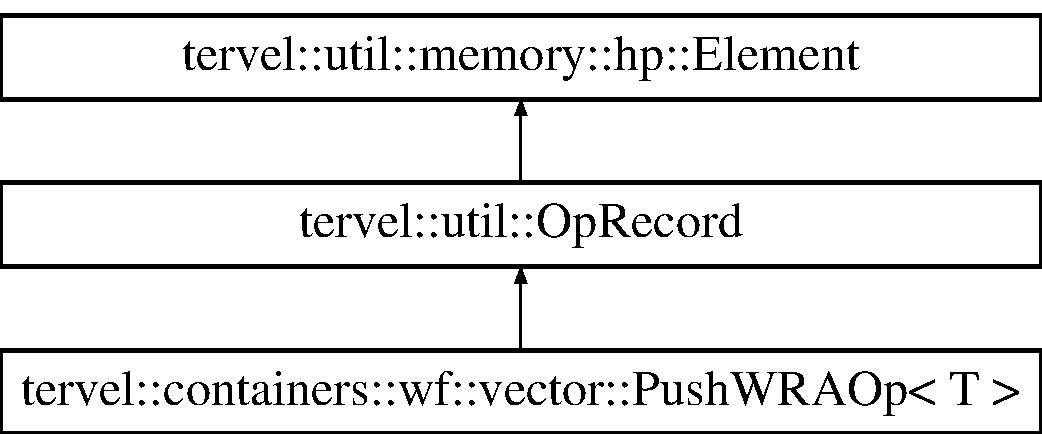
\includegraphics[height=3.000000cm]{classtervel_1_1containers_1_1wf_1_1vector_1_1_push_w_r_a_op}
\end{center}
\end{figure}
\subsection*{Public Member Functions}
\begin{DoxyCompactItemize}
\item 
\hyperlink{classtervel_1_1containers_1_1wf_1_1vector_1_1_push_w_r_a_op_a404988cf99e2e7c243554bf89724aa55}{Push\+W\+R\+A\+Op} (Vector$<$ T $>$ $\ast$vec, T val)
\item 
\hyperlink{classtervel_1_1containers_1_1wf_1_1vector_1_1_push_w_r_a_op_a6a79e2d4818ff9ffccb7f51130e6bd67}{$\sim$\+Push\+W\+R\+A\+Op} ()
\item 
void \hyperlink{classtervel_1_1containers_1_1wf_1_1vector_1_1_push_w_r_a_op_ae06dc17442f24775407ce7eabbf79a59}{help\+\_\+complete} ()
\begin{DoxyCompactList}\small\item\em Implementations of this function that upon its return the operation described in the Op\+Record has been completed. \end{DoxyCompactList}\item 
uint64\+\_\+t \hyperlink{classtervel_1_1containers_1_1wf_1_1vector_1_1_push_w_r_a_op_ae27b39abee8d9f4568f1219ca34a0bc5}{result} ()
\end{DoxyCompactItemize}
\subsection*{Private Attributes}
\begin{DoxyCompactItemize}
\item 
Vector$<$ T $>$ $\ast$ \hyperlink{classtervel_1_1containers_1_1wf_1_1vector_1_1_push_w_r_a_op_ae68e6c5e445fcf86aee12bc6e2d1f6bf}{vec\+\_\+}
\item 
T \hyperlink{classtervel_1_1containers_1_1wf_1_1vector_1_1_push_w_r_a_op_adf7e228b9e370014c79aec8a628a6cb8}{new\+\_\+val\+\_\+}
\item 
std\+::atomic$<$ \hyperlink{classtervel_1_1containers_1_1wf_1_1vector_1_1_push_w_r_a_op_helper}{Push\+W\+R\+A\+Op\+Helper}$<$ T $>$ $\ast$ $>$ \hyperlink{classtervel_1_1containers_1_1wf_1_1vector_1_1_push_w_r_a_op_a11858ec4a2c535d4c7a638b701b1011e}{helper\+\_\+} \{nullptr\}
\end{DoxyCompactItemize}
\subsection*{Friends}
\begin{DoxyCompactItemize}
\item 
class \hyperlink{classtervel_1_1containers_1_1wf_1_1vector_1_1_push_w_r_a_op_af5b4dff870a0a3fb9ebf7b76ab2143f1}{Push\+W\+R\+A\+Op\+Helper$<$ T $>$}
\end{DoxyCompactItemize}


\subsection{Constructor \& Destructor Documentation}
\hypertarget{classtervel_1_1containers_1_1wf_1_1vector_1_1_push_w_r_a_op_a404988cf99e2e7c243554bf89724aa55}{}\index{tervel\+::containers\+::wf\+::vector\+::\+Push\+W\+R\+A\+Op@{tervel\+::containers\+::wf\+::vector\+::\+Push\+W\+R\+A\+Op}!Push\+W\+R\+A\+Op@{Push\+W\+R\+A\+Op}}
\index{Push\+W\+R\+A\+Op@{Push\+W\+R\+A\+Op}!tervel\+::containers\+::wf\+::vector\+::\+Push\+W\+R\+A\+Op@{tervel\+::containers\+::wf\+::vector\+::\+Push\+W\+R\+A\+Op}}
\subsubsection[{Push\+W\+R\+A\+Op(\+Vector$<$ T $>$ $\ast$vec, T val)}]{\setlength{\rightskip}{0pt plus 5cm}template$<$typename T$>$ {\bf tervel\+::containers\+::wf\+::vector\+::\+Push\+W\+R\+A\+Op}$<$ T $>$\+::{\bf Push\+W\+R\+A\+Op} (
\begin{DoxyParamCaption}
\item[{Vector$<$ T $>$ $\ast$}]{vec, }
\item[{T}]{val}
\end{DoxyParamCaption}
)\hspace{0.3cm}{\ttfamily [inline]}}\label{classtervel_1_1containers_1_1wf_1_1vector_1_1_push_w_r_a_op_a404988cf99e2e7c243554bf89724aa55}
\hypertarget{classtervel_1_1containers_1_1wf_1_1vector_1_1_push_w_r_a_op_a6a79e2d4818ff9ffccb7f51130e6bd67}{}\index{tervel\+::containers\+::wf\+::vector\+::\+Push\+W\+R\+A\+Op@{tervel\+::containers\+::wf\+::vector\+::\+Push\+W\+R\+A\+Op}!````~Push\+W\+R\+A\+Op@{$\sim$\+Push\+W\+R\+A\+Op}}
\index{````~Push\+W\+R\+A\+Op@{$\sim$\+Push\+W\+R\+A\+Op}!tervel\+::containers\+::wf\+::vector\+::\+Push\+W\+R\+A\+Op@{tervel\+::containers\+::wf\+::vector\+::\+Push\+W\+R\+A\+Op}}
\subsubsection[{$\sim$\+Push\+W\+R\+A\+Op()}]{\setlength{\rightskip}{0pt plus 5cm}template$<$typename T$>$ {\bf tervel\+::containers\+::wf\+::vector\+::\+Push\+W\+R\+A\+Op}$<$ T $>$\+::$\sim${\bf Push\+W\+R\+A\+Op} (
\begin{DoxyParamCaption}
{}
\end{DoxyParamCaption}
)\hspace{0.3cm}{\ttfamily [inline]}}\label{classtervel_1_1containers_1_1wf_1_1vector_1_1_push_w_r_a_op_a6a79e2d4818ff9ffccb7f51130e6bd67}


\subsection{Member Function Documentation}
\hypertarget{classtervel_1_1containers_1_1wf_1_1vector_1_1_push_w_r_a_op_ae06dc17442f24775407ce7eabbf79a59}{}\index{tervel\+::containers\+::wf\+::vector\+::\+Push\+W\+R\+A\+Op@{tervel\+::containers\+::wf\+::vector\+::\+Push\+W\+R\+A\+Op}!help\+\_\+complete@{help\+\_\+complete}}
\index{help\+\_\+complete@{help\+\_\+complete}!tervel\+::containers\+::wf\+::vector\+::\+Push\+W\+R\+A\+Op@{tervel\+::containers\+::wf\+::vector\+::\+Push\+W\+R\+A\+Op}}
\subsubsection[{help\+\_\+complete()}]{\setlength{\rightskip}{0pt plus 5cm}template$<$typename T$>$ void {\bf tervel\+::containers\+::wf\+::vector\+::\+Push\+W\+R\+A\+Op}$<$ T $>$\+::help\+\_\+complete (
\begin{DoxyParamCaption}
{}
\end{DoxyParamCaption}
)\hspace{0.3cm}{\ttfamily [inline]}, {\ttfamily [virtual]}}\label{classtervel_1_1containers_1_1wf_1_1vector_1_1_push_w_r_a_op_ae06dc17442f24775407ce7eabbf79a59}


Implementations of this function that upon its return the operation described in the Op\+Record has been completed. 

As such it must be thread-\/safe and the extending class must contain all the information necessary to complete the operation. 

Implements \hyperlink{classtervel_1_1util_1_1_op_record_aa75ab39688a8d4cceb6a1ef0409537c0}{tervel\+::util\+::\+Op\+Record}.

\hypertarget{classtervel_1_1containers_1_1wf_1_1vector_1_1_push_w_r_a_op_ae27b39abee8d9f4568f1219ca34a0bc5}{}\index{tervel\+::containers\+::wf\+::vector\+::\+Push\+W\+R\+A\+Op@{tervel\+::containers\+::wf\+::vector\+::\+Push\+W\+R\+A\+Op}!result@{result}}
\index{result@{result}!tervel\+::containers\+::wf\+::vector\+::\+Push\+W\+R\+A\+Op@{tervel\+::containers\+::wf\+::vector\+::\+Push\+W\+R\+A\+Op}}
\subsubsection[{result()}]{\setlength{\rightskip}{0pt plus 5cm}template$<$typename T$>$ uint64\+\_\+t {\bf tervel\+::containers\+::wf\+::vector\+::\+Push\+W\+R\+A\+Op}$<$ T $>$\+::result (
\begin{DoxyParamCaption}
{}
\end{DoxyParamCaption}
)\hspace{0.3cm}{\ttfamily [inline]}}\label{classtervel_1_1containers_1_1wf_1_1vector_1_1_push_w_r_a_op_ae27b39abee8d9f4568f1219ca34a0bc5}


\subsection{Friends And Related Function Documentation}
\hypertarget{classtervel_1_1containers_1_1wf_1_1vector_1_1_push_w_r_a_op_af5b4dff870a0a3fb9ebf7b76ab2143f1}{}\index{tervel\+::containers\+::wf\+::vector\+::\+Push\+W\+R\+A\+Op@{tervel\+::containers\+::wf\+::vector\+::\+Push\+W\+R\+A\+Op}!Push\+W\+R\+A\+Op\+Helper$<$ T $>$@{Push\+W\+R\+A\+Op\+Helper$<$ T $>$}}
\index{Push\+W\+R\+A\+Op\+Helper$<$ T $>$@{Push\+W\+R\+A\+Op\+Helper$<$ T $>$}!tervel\+::containers\+::wf\+::vector\+::\+Push\+W\+R\+A\+Op@{tervel\+::containers\+::wf\+::vector\+::\+Push\+W\+R\+A\+Op}}
\subsubsection[{Push\+W\+R\+A\+Op\+Helper$<$ T $>$}]{\setlength{\rightskip}{0pt plus 5cm}template$<$typename T$>$ friend class {\bf Push\+W\+R\+A\+Op\+Helper}$<$ T $>$\hspace{0.3cm}{\ttfamily [friend]}}\label{classtervel_1_1containers_1_1wf_1_1vector_1_1_push_w_r_a_op_af5b4dff870a0a3fb9ebf7b76ab2143f1}


\subsection{Member Data Documentation}
\hypertarget{classtervel_1_1containers_1_1wf_1_1vector_1_1_push_w_r_a_op_a11858ec4a2c535d4c7a638b701b1011e}{}\index{tervel\+::containers\+::wf\+::vector\+::\+Push\+W\+R\+A\+Op@{tervel\+::containers\+::wf\+::vector\+::\+Push\+W\+R\+A\+Op}!helper\+\_\+@{helper\+\_\+}}
\index{helper\+\_\+@{helper\+\_\+}!tervel\+::containers\+::wf\+::vector\+::\+Push\+W\+R\+A\+Op@{tervel\+::containers\+::wf\+::vector\+::\+Push\+W\+R\+A\+Op}}
\subsubsection[{helper\+\_\+}]{\setlength{\rightskip}{0pt plus 5cm}template$<$typename T$>$ std\+::atomic$<${\bf Push\+W\+R\+A\+Op\+Helper}$<$T$>$ $\ast$$>$ {\bf tervel\+::containers\+::wf\+::vector\+::\+Push\+W\+R\+A\+Op}$<$ T $>$\+::helper\+\_\+ \{nullptr\}\hspace{0.3cm}{\ttfamily [private]}}\label{classtervel_1_1containers_1_1wf_1_1vector_1_1_push_w_r_a_op_a11858ec4a2c535d4c7a638b701b1011e}
\hypertarget{classtervel_1_1containers_1_1wf_1_1vector_1_1_push_w_r_a_op_adf7e228b9e370014c79aec8a628a6cb8}{}\index{tervel\+::containers\+::wf\+::vector\+::\+Push\+W\+R\+A\+Op@{tervel\+::containers\+::wf\+::vector\+::\+Push\+W\+R\+A\+Op}!new\+\_\+val\+\_\+@{new\+\_\+val\+\_\+}}
\index{new\+\_\+val\+\_\+@{new\+\_\+val\+\_\+}!tervel\+::containers\+::wf\+::vector\+::\+Push\+W\+R\+A\+Op@{tervel\+::containers\+::wf\+::vector\+::\+Push\+W\+R\+A\+Op}}
\subsubsection[{new\+\_\+val\+\_\+}]{\setlength{\rightskip}{0pt plus 5cm}template$<$typename T$>$ T {\bf tervel\+::containers\+::wf\+::vector\+::\+Push\+W\+R\+A\+Op}$<$ T $>$\+::new\+\_\+val\+\_\+\hspace{0.3cm}{\ttfamily [private]}}\label{classtervel_1_1containers_1_1wf_1_1vector_1_1_push_w_r_a_op_adf7e228b9e370014c79aec8a628a6cb8}
\hypertarget{classtervel_1_1containers_1_1wf_1_1vector_1_1_push_w_r_a_op_ae68e6c5e445fcf86aee12bc6e2d1f6bf}{}\index{tervel\+::containers\+::wf\+::vector\+::\+Push\+W\+R\+A\+Op@{tervel\+::containers\+::wf\+::vector\+::\+Push\+W\+R\+A\+Op}!vec\+\_\+@{vec\+\_\+}}
\index{vec\+\_\+@{vec\+\_\+}!tervel\+::containers\+::wf\+::vector\+::\+Push\+W\+R\+A\+Op@{tervel\+::containers\+::wf\+::vector\+::\+Push\+W\+R\+A\+Op}}
\subsubsection[{vec\+\_\+}]{\setlength{\rightskip}{0pt plus 5cm}template$<$typename T$>$ Vector$<$T$>$$\ast$ {\bf tervel\+::containers\+::wf\+::vector\+::\+Push\+W\+R\+A\+Op}$<$ T $>$\+::vec\+\_\+\hspace{0.3cm}{\ttfamily [private]}}\label{classtervel_1_1containers_1_1wf_1_1vector_1_1_push_w_r_a_op_ae68e6c5e445fcf86aee12bc6e2d1f6bf}


The documentation for this class was generated from the following file\+:\begin{DoxyCompactItemize}
\item 
tervel/containers/wf/vector/\hyperlink{pushbackwra__op_8h}{pushbackwra\+\_\+op.\+h}\end{DoxyCompactItemize}

\hypertarget{classtervel_1_1containers_1_1wf_1_1vector_1_1_push_w_r_a_op_helper}{}\section{tervel\+:\+:containers\+:\+:wf\+:\+:vector\+:\+:Push\+W\+R\+A\+Op\+Helper$<$ T $>$ Class Template Reference}
\label{classtervel_1_1containers_1_1wf_1_1vector_1_1_push_w_r_a_op_helper}\index{tervel\+::containers\+::wf\+::vector\+::\+Push\+W\+R\+A\+Op\+Helper$<$ T $>$@{tervel\+::containers\+::wf\+::vector\+::\+Push\+W\+R\+A\+Op\+Helper$<$ T $>$}}


{\ttfamily \#include $<$pushbackwra\+\_\+op.\+h$>$}

Inheritance diagram for tervel\+:\+:containers\+:\+:wf\+:\+:vector\+:\+:Push\+W\+R\+A\+Op\+Helper$<$ T $>$\+:\begin{figure}[H]
\begin{center}
\leavevmode
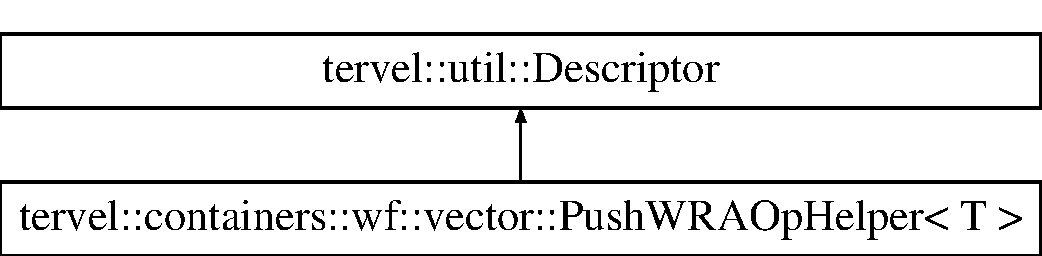
\includegraphics[height=2.000000cm]{classtervel_1_1containers_1_1wf_1_1vector_1_1_push_w_r_a_op_helper}
\end{center}
\end{figure}
\subsection*{Public Member Functions}
\begin{DoxyCompactItemize}
\item 
\hyperlink{classtervel_1_1containers_1_1wf_1_1vector_1_1_push_w_r_a_op_helper_a3fe26df430b7d5a1102f6871e1166a85}{Push\+W\+R\+A\+Op\+Helper} (\hyperlink{classtervel_1_1containers_1_1wf_1_1vector_1_1_push_w_r_a_op}{Push\+W\+R\+A\+Op}$<$ T $>$ $\ast$op)
\item 
void \hyperlink{classtervel_1_1containers_1_1wf_1_1vector_1_1_push_w_r_a_op_helper_a368ab8ad0b4b8470b201995a6f12a226}{set\+\_\+idx} (uint64\+\_\+t i)
\item 
uint64\+\_\+t \hyperlink{classtervel_1_1containers_1_1wf_1_1vector_1_1_push_w_r_a_op_helper_a9b08e8d16012894c0ec04aa92bbde2d1}{idx} ()
\item 
bool \hyperlink{classtervel_1_1containers_1_1wf_1_1vector_1_1_push_w_r_a_op_helper_ab72ec790d16af1a786039289a61e135e}{result} ()
\item 
bool \hyperlink{classtervel_1_1containers_1_1wf_1_1vector_1_1_push_w_r_a_op_helper_aea01bbb42a32ca5bb4d0a27c9158c81a}{associate} ()
\item 
void $\ast$ \hyperlink{classtervel_1_1containers_1_1wf_1_1vector_1_1_push_w_r_a_op_helper_a77a582be1e79950c4de106e031d5fa1c}{complete} (void $\ast$value, std\+::atomic$<$ void $\ast$ $>$ $\ast$address)
\begin{DoxyCompactList}\small\item\em This method is implemented by each sub class and must guarantee that upon return that the descriptor no longer exists at the address it was placed. \end{DoxyCompactList}\item 
void $\ast$ \hyperlink{classtervel_1_1containers_1_1wf_1_1vector_1_1_push_w_r_a_op_helper_a2c1c6135378bd516be4a147d7e9a61a5}{get\+\_\+logical\+\_\+value} ()
\begin{DoxyCompactList}\small\item\em This method is implemented by each sub class. \end{DoxyCompactList}\item 
bool \hyperlink{classtervel_1_1containers_1_1wf_1_1vector_1_1_push_w_r_a_op_helper_ab330b531d19d3ef8c8b86e239ce22215}{on\+\_\+watch} (std\+::atomic$<$ void $\ast$ $>$ $\ast$address, void $\ast$value)
\begin{DoxyCompactList}\small\item\em This method is optional to implement for each sub class. \end{DoxyCompactList}\end{DoxyCompactItemize}
\subsection*{Private Attributes}
\begin{DoxyCompactItemize}
\item 
\hyperlink{classtervel_1_1containers_1_1wf_1_1vector_1_1_push_w_r_a_op}{Push\+W\+R\+A\+Op}$<$ T $>$ $\ast$ \hyperlink{classtervel_1_1containers_1_1wf_1_1vector_1_1_push_w_r_a_op_helper_adcb96f369c052a709fa3b2a5ea12d642}{op\+\_\+}
\item 
uint64\+\_\+t \hyperlink{classtervel_1_1containers_1_1wf_1_1vector_1_1_push_w_r_a_op_helper_a059176bc02e87fbbe4fe344ef63630ea}{idx\+\_\+}
\end{DoxyCompactItemize}
\subsection*{Friends}
\begin{DoxyCompactItemize}
\item 
class \hyperlink{classtervel_1_1containers_1_1wf_1_1vector_1_1_push_w_r_a_op_helper_a55dec9ce6e1993f721d73ecd1741dc33}{Push\+W\+R\+A\+Op$<$ T $>$}
\end{DoxyCompactItemize}


\subsection{Constructor \& Destructor Documentation}
\hypertarget{classtervel_1_1containers_1_1wf_1_1vector_1_1_push_w_r_a_op_helper_a3fe26df430b7d5a1102f6871e1166a85}{}\index{tervel\+::containers\+::wf\+::vector\+::\+Push\+W\+R\+A\+Op\+Helper@{tervel\+::containers\+::wf\+::vector\+::\+Push\+W\+R\+A\+Op\+Helper}!Push\+W\+R\+A\+Op\+Helper@{Push\+W\+R\+A\+Op\+Helper}}
\index{Push\+W\+R\+A\+Op\+Helper@{Push\+W\+R\+A\+Op\+Helper}!tervel\+::containers\+::wf\+::vector\+::\+Push\+W\+R\+A\+Op\+Helper@{tervel\+::containers\+::wf\+::vector\+::\+Push\+W\+R\+A\+Op\+Helper}}
\subsubsection[{Push\+W\+R\+A\+Op\+Helper(\+Push\+W\+R\+A\+Op$<$ T $>$ $\ast$op)}]{\setlength{\rightskip}{0pt plus 5cm}template$<$typename T$>$ {\bf tervel\+::containers\+::wf\+::vector\+::\+Push\+W\+R\+A\+Op\+Helper}$<$ T $>$\+::{\bf Push\+W\+R\+A\+Op\+Helper} (
\begin{DoxyParamCaption}
\item[{{\bf Push\+W\+R\+A\+Op}$<$ T $>$ $\ast$}]{op}
\end{DoxyParamCaption}
)\hspace{0.3cm}{\ttfamily [inline]}, {\ttfamily [explicit]}}\label{classtervel_1_1containers_1_1wf_1_1vector_1_1_push_w_r_a_op_helper_a3fe26df430b7d5a1102f6871e1166a85}


\subsection{Member Function Documentation}
\hypertarget{classtervel_1_1containers_1_1wf_1_1vector_1_1_push_w_r_a_op_helper_aea01bbb42a32ca5bb4d0a27c9158c81a}{}\index{tervel\+::containers\+::wf\+::vector\+::\+Push\+W\+R\+A\+Op\+Helper@{tervel\+::containers\+::wf\+::vector\+::\+Push\+W\+R\+A\+Op\+Helper}!associate@{associate}}
\index{associate@{associate}!tervel\+::containers\+::wf\+::vector\+::\+Push\+W\+R\+A\+Op\+Helper@{tervel\+::containers\+::wf\+::vector\+::\+Push\+W\+R\+A\+Op\+Helper}}
\subsubsection[{associate()}]{\setlength{\rightskip}{0pt plus 5cm}template$<$typename T$>$ bool {\bf tervel\+::containers\+::wf\+::vector\+::\+Push\+W\+R\+A\+Op\+Helper}$<$ T $>$\+::associate (
\begin{DoxyParamCaption}
{}
\end{DoxyParamCaption}
)\hspace{0.3cm}{\ttfamily [inline]}}\label{classtervel_1_1containers_1_1wf_1_1vector_1_1_push_w_r_a_op_helper_aea01bbb42a32ca5bb4d0a27c9158c81a}
\hypertarget{classtervel_1_1containers_1_1wf_1_1vector_1_1_push_w_r_a_op_helper_a77a582be1e79950c4de106e031d5fa1c}{}\index{tervel\+::containers\+::wf\+::vector\+::\+Push\+W\+R\+A\+Op\+Helper@{tervel\+::containers\+::wf\+::vector\+::\+Push\+W\+R\+A\+Op\+Helper}!complete@{complete}}
\index{complete@{complete}!tervel\+::containers\+::wf\+::vector\+::\+Push\+W\+R\+A\+Op\+Helper@{tervel\+::containers\+::wf\+::vector\+::\+Push\+W\+R\+A\+Op\+Helper}}
\subsubsection[{complete(void $\ast$value, std\+::atomic$<$ void $\ast$ $>$ $\ast$address)}]{\setlength{\rightskip}{0pt plus 5cm}template$<$typename T$>$ void$\ast$ {\bf tervel\+::containers\+::wf\+::vector\+::\+Push\+W\+R\+A\+Op\+Helper}$<$ T $>$\+::complete (
\begin{DoxyParamCaption}
\item[{void $\ast$}]{current, }
\item[{std\+::atomic$<$ void $\ast$ $>$ $\ast$}]{address}
\end{DoxyParamCaption}
)\hspace{0.3cm}{\ttfamily [inline]}, {\ttfamily [virtual]}}\label{classtervel_1_1containers_1_1wf_1_1vector_1_1_push_w_r_a_op_helper_a77a582be1e79950c4de106e031d5fa1c}


This method is implemented by each sub class and must guarantee that upon return that the descriptor no longer exists at the address it was placed. 


\begin{DoxyParams}{Parameters}
{\em current} & the reference to this object as it is at the address, \\
\hline
{\em address} & the location this object was read from \\
\hline
\end{DoxyParams}


Implements \hyperlink{classtervel_1_1util_1_1_descriptor_a4303b2a08e3ab67de5533cfb20db87c9}{tervel\+::util\+::\+Descriptor}.

\hypertarget{classtervel_1_1containers_1_1wf_1_1vector_1_1_push_w_r_a_op_helper_a2c1c6135378bd516be4a147d7e9a61a5}{}\index{tervel\+::containers\+::wf\+::vector\+::\+Push\+W\+R\+A\+Op\+Helper@{tervel\+::containers\+::wf\+::vector\+::\+Push\+W\+R\+A\+Op\+Helper}!get\+\_\+logical\+\_\+value@{get\+\_\+logical\+\_\+value}}
\index{get\+\_\+logical\+\_\+value@{get\+\_\+logical\+\_\+value}!tervel\+::containers\+::wf\+::vector\+::\+Push\+W\+R\+A\+Op\+Helper@{tervel\+::containers\+::wf\+::vector\+::\+Push\+W\+R\+A\+Op\+Helper}}
\subsubsection[{get\+\_\+logical\+\_\+value()}]{\setlength{\rightskip}{0pt plus 5cm}template$<$typename T$>$ void$\ast$ {\bf tervel\+::containers\+::wf\+::vector\+::\+Push\+W\+R\+A\+Op\+Helper}$<$ T $>$\+::get\+\_\+logical\+\_\+value (
\begin{DoxyParamCaption}
{}
\end{DoxyParamCaption}
)\hspace{0.3cm}{\ttfamily [inline]}, {\ttfamily [virtual]}}\label{classtervel_1_1containers_1_1wf_1_1vector_1_1_push_w_r_a_op_helper_a2c1c6135378bd516be4a147d7e9a61a5}


This method is implemented by each sub class. 

It returns the logical value of the past address. If the associated operation is still in progress then it will generally return the value that was replaced by this descriptor. Otherwise it will generally return the result of the operation for the specified address.

It can only be called from the static function which protects the object from being reused during the function. 

Implements \hyperlink{classtervel_1_1util_1_1_descriptor_a5b443eeb6acf1207f27a6d06c39d4ad4}{tervel\+::util\+::\+Descriptor}.

\hypertarget{classtervel_1_1containers_1_1wf_1_1vector_1_1_push_w_r_a_op_helper_a9b08e8d16012894c0ec04aa92bbde2d1}{}\index{tervel\+::containers\+::wf\+::vector\+::\+Push\+W\+R\+A\+Op\+Helper@{tervel\+::containers\+::wf\+::vector\+::\+Push\+W\+R\+A\+Op\+Helper}!idx@{idx}}
\index{idx@{idx}!tervel\+::containers\+::wf\+::vector\+::\+Push\+W\+R\+A\+Op\+Helper@{tervel\+::containers\+::wf\+::vector\+::\+Push\+W\+R\+A\+Op\+Helper}}
\subsubsection[{idx()}]{\setlength{\rightskip}{0pt plus 5cm}template$<$typename T$>$ uint64\+\_\+t {\bf tervel\+::containers\+::wf\+::vector\+::\+Push\+W\+R\+A\+Op\+Helper}$<$ T $>$\+::idx (
\begin{DoxyParamCaption}
{}
\end{DoxyParamCaption}
)\hspace{0.3cm}{\ttfamily [inline]}}\label{classtervel_1_1containers_1_1wf_1_1vector_1_1_push_w_r_a_op_helper_a9b08e8d16012894c0ec04aa92bbde2d1}
\hypertarget{classtervel_1_1containers_1_1wf_1_1vector_1_1_push_w_r_a_op_helper_ab330b531d19d3ef8c8b86e239ce22215}{}\index{tervel\+::containers\+::wf\+::vector\+::\+Push\+W\+R\+A\+Op\+Helper@{tervel\+::containers\+::wf\+::vector\+::\+Push\+W\+R\+A\+Op\+Helper}!on\+\_\+watch@{on\+\_\+watch}}
\index{on\+\_\+watch@{on\+\_\+watch}!tervel\+::containers\+::wf\+::vector\+::\+Push\+W\+R\+A\+Op\+Helper@{tervel\+::containers\+::wf\+::vector\+::\+Push\+W\+R\+A\+Op\+Helper}}
\subsubsection[{on\+\_\+watch(std\+::atomic$<$ void $\ast$ $>$ $\ast$address, void $\ast$value)}]{\setlength{\rightskip}{0pt plus 5cm}template$<$typename T$>$ bool {\bf tervel\+::containers\+::wf\+::vector\+::\+Push\+W\+R\+A\+Op\+Helper}$<$ T $>$\+::on\+\_\+watch (
\begin{DoxyParamCaption}
\item[{std\+::atomic$<$ void $\ast$ $>$ $\ast$}]{, }
\item[{void $\ast$}]{}
\end{DoxyParamCaption}
)\hspace{0.3cm}{\ttfamily [inline]}, {\ttfamily [virtual]}}\label{classtervel_1_1containers_1_1wf_1_1vector_1_1_push_w_r_a_op_helper_ab330b531d19d3ef8c8b86e239ce22215}


This method is optional to implement for each sub class. 

In the event there is a complex dependency between descriptor objects, where watching one implies performing other actions, such as watching a parent object, a developer will implement this function to encapsulate that logic

This function is called by the static watch function It should not watch itself.


\begin{DoxyParams}{Parameters}
{\em address} & The location to check. \\
\hline
{\em expected} & The expected value for that location\\
\hline
\end{DoxyParams}
\begin{DoxyReturn}{Returns}
true if successful, false otherwise 
\end{DoxyReturn}


Reimplemented from \hyperlink{classtervel_1_1util_1_1_descriptor_ab643e09f20f35149dc820766b0f9ccdb}{tervel\+::util\+::\+Descriptor}.

\hypertarget{classtervel_1_1containers_1_1wf_1_1vector_1_1_push_w_r_a_op_helper_ab72ec790d16af1a786039289a61e135e}{}\index{tervel\+::containers\+::wf\+::vector\+::\+Push\+W\+R\+A\+Op\+Helper@{tervel\+::containers\+::wf\+::vector\+::\+Push\+W\+R\+A\+Op\+Helper}!result@{result}}
\index{result@{result}!tervel\+::containers\+::wf\+::vector\+::\+Push\+W\+R\+A\+Op\+Helper@{tervel\+::containers\+::wf\+::vector\+::\+Push\+W\+R\+A\+Op\+Helper}}
\subsubsection[{result()}]{\setlength{\rightskip}{0pt plus 5cm}template$<$typename T$>$ bool {\bf tervel\+::containers\+::wf\+::vector\+::\+Push\+W\+R\+A\+Op\+Helper}$<$ T $>$\+::result (
\begin{DoxyParamCaption}
{}
\end{DoxyParamCaption}
)\hspace{0.3cm}{\ttfamily [inline]}}\label{classtervel_1_1containers_1_1wf_1_1vector_1_1_push_w_r_a_op_helper_ab72ec790d16af1a786039289a61e135e}
\hypertarget{classtervel_1_1containers_1_1wf_1_1vector_1_1_push_w_r_a_op_helper_a368ab8ad0b4b8470b201995a6f12a226}{}\index{tervel\+::containers\+::wf\+::vector\+::\+Push\+W\+R\+A\+Op\+Helper@{tervel\+::containers\+::wf\+::vector\+::\+Push\+W\+R\+A\+Op\+Helper}!set\+\_\+idx@{set\+\_\+idx}}
\index{set\+\_\+idx@{set\+\_\+idx}!tervel\+::containers\+::wf\+::vector\+::\+Push\+W\+R\+A\+Op\+Helper@{tervel\+::containers\+::wf\+::vector\+::\+Push\+W\+R\+A\+Op\+Helper}}
\subsubsection[{set\+\_\+idx(uint64\+\_\+t i)}]{\setlength{\rightskip}{0pt plus 5cm}template$<$typename T$>$ void {\bf tervel\+::containers\+::wf\+::vector\+::\+Push\+W\+R\+A\+Op\+Helper}$<$ T $>$\+::set\+\_\+idx (
\begin{DoxyParamCaption}
\item[{uint64\+\_\+t}]{i}
\end{DoxyParamCaption}
)\hspace{0.3cm}{\ttfamily [inline]}}\label{classtervel_1_1containers_1_1wf_1_1vector_1_1_push_w_r_a_op_helper_a368ab8ad0b4b8470b201995a6f12a226}


\subsection{Friends And Related Function Documentation}
\hypertarget{classtervel_1_1containers_1_1wf_1_1vector_1_1_push_w_r_a_op_helper_a55dec9ce6e1993f721d73ecd1741dc33}{}\index{tervel\+::containers\+::wf\+::vector\+::\+Push\+W\+R\+A\+Op\+Helper@{tervel\+::containers\+::wf\+::vector\+::\+Push\+W\+R\+A\+Op\+Helper}!Push\+W\+R\+A\+Op$<$ T $>$@{Push\+W\+R\+A\+Op$<$ T $>$}}
\index{Push\+W\+R\+A\+Op$<$ T $>$@{Push\+W\+R\+A\+Op$<$ T $>$}!tervel\+::containers\+::wf\+::vector\+::\+Push\+W\+R\+A\+Op\+Helper@{tervel\+::containers\+::wf\+::vector\+::\+Push\+W\+R\+A\+Op\+Helper}}
\subsubsection[{Push\+W\+R\+A\+Op$<$ T $>$}]{\setlength{\rightskip}{0pt plus 5cm}template$<$typename T$>$ friend class {\bf Push\+W\+R\+A\+Op}$<$ T $>$\hspace{0.3cm}{\ttfamily [friend]}}\label{classtervel_1_1containers_1_1wf_1_1vector_1_1_push_w_r_a_op_helper_a55dec9ce6e1993f721d73ecd1741dc33}


\subsection{Member Data Documentation}
\hypertarget{classtervel_1_1containers_1_1wf_1_1vector_1_1_push_w_r_a_op_helper_a059176bc02e87fbbe4fe344ef63630ea}{}\index{tervel\+::containers\+::wf\+::vector\+::\+Push\+W\+R\+A\+Op\+Helper@{tervel\+::containers\+::wf\+::vector\+::\+Push\+W\+R\+A\+Op\+Helper}!idx\+\_\+@{idx\+\_\+}}
\index{idx\+\_\+@{idx\+\_\+}!tervel\+::containers\+::wf\+::vector\+::\+Push\+W\+R\+A\+Op\+Helper@{tervel\+::containers\+::wf\+::vector\+::\+Push\+W\+R\+A\+Op\+Helper}}
\subsubsection[{idx\+\_\+}]{\setlength{\rightskip}{0pt plus 5cm}template$<$typename T$>$ uint64\+\_\+t {\bf tervel\+::containers\+::wf\+::vector\+::\+Push\+W\+R\+A\+Op\+Helper}$<$ T $>$\+::idx\+\_\+\hspace{0.3cm}{\ttfamily [private]}}\label{classtervel_1_1containers_1_1wf_1_1vector_1_1_push_w_r_a_op_helper_a059176bc02e87fbbe4fe344ef63630ea}
\hypertarget{classtervel_1_1containers_1_1wf_1_1vector_1_1_push_w_r_a_op_helper_adcb96f369c052a709fa3b2a5ea12d642}{}\index{tervel\+::containers\+::wf\+::vector\+::\+Push\+W\+R\+A\+Op\+Helper@{tervel\+::containers\+::wf\+::vector\+::\+Push\+W\+R\+A\+Op\+Helper}!op\+\_\+@{op\+\_\+}}
\index{op\+\_\+@{op\+\_\+}!tervel\+::containers\+::wf\+::vector\+::\+Push\+W\+R\+A\+Op\+Helper@{tervel\+::containers\+::wf\+::vector\+::\+Push\+W\+R\+A\+Op\+Helper}}
\subsubsection[{op\+\_\+}]{\setlength{\rightskip}{0pt plus 5cm}template$<$typename T$>$ {\bf Push\+W\+R\+A\+Op}$<$T$>$$\ast$ {\bf tervel\+::containers\+::wf\+::vector\+::\+Push\+W\+R\+A\+Op\+Helper}$<$ T $>$\+::op\+\_\+\hspace{0.3cm}{\ttfamily [private]}}\label{classtervel_1_1containers_1_1wf_1_1vector_1_1_push_w_r_a_op_helper_adcb96f369c052a709fa3b2a5ea12d642}


The documentation for this class was generated from the following file\+:\begin{DoxyCompactItemize}
\item 
tervel/containers/wf/vector/\hyperlink{pushbackwra__op_8h}{pushbackwra\+\_\+op.\+h}\end{DoxyCompactItemize}

\hypertarget{classtervel_1_1util_1_1memory_1_1rc_1_1_read_first_op}{}\section{tervel\+:\+:util\+:\+:memory\+:\+:rc\+:\+:Read\+First\+Op Class Reference}
\label{classtervel_1_1util_1_1memory_1_1rc_1_1_read_first_op}\index{tervel\+::util\+::memory\+::rc\+::\+Read\+First\+Op@{tervel\+::util\+::memory\+::rc\+::\+Read\+First\+Op}}


Class used for placement in the Op Table to complete an operation that failed to complete in a bounded number of steps.  




{\ttfamily \#include $<$descriptor\+\_\+read\+\_\+first\+\_\+op.\+h$>$}

Inheritance diagram for tervel\+:\+:util\+:\+:memory\+:\+:rc\+:\+:Read\+First\+Op\+:\begin{figure}[H]
\begin{center}
\leavevmode
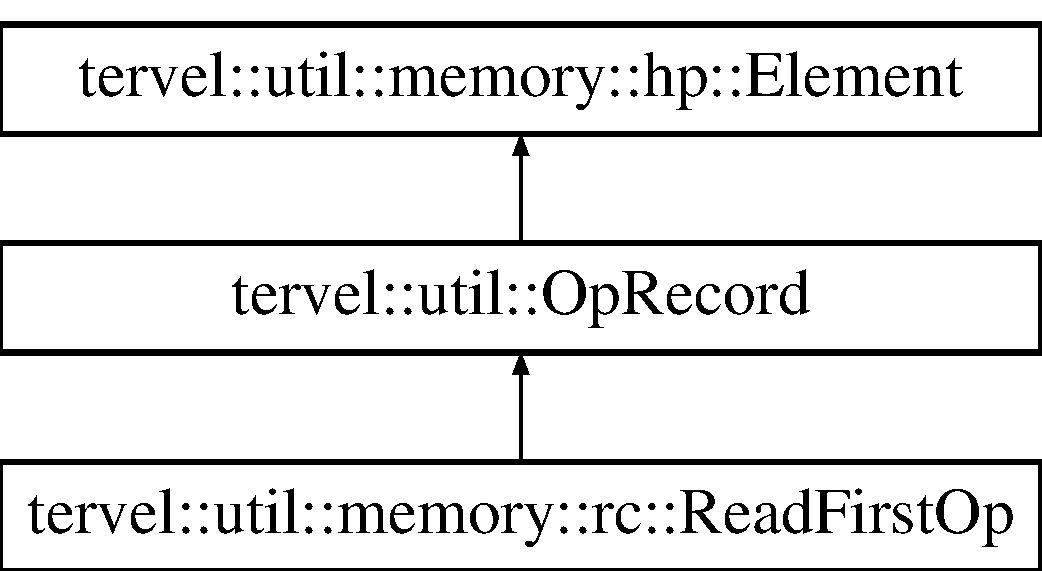
\includegraphics[height=3.000000cm]{classtervel_1_1util_1_1memory_1_1rc_1_1_read_first_op}
\end{center}
\end{figure}
\subsection*{Public Member Functions}
\begin{DoxyCompactItemize}
\item 
\hyperlink{classtervel_1_1util_1_1memory_1_1rc_1_1_read_first_op_af7cc3260ed88464d0582506c90213ca3}{Read\+First\+Op} (std\+::atomic$<$ void $\ast$ $>$ $\ast$address)
\item 
\hyperlink{classtervel_1_1util_1_1memory_1_1rc_1_1_read_first_op_a7d2703263cf845895cf8523343a44f5a}{$\sim$\+Read\+First\+Op} ()
\item 
void \hyperlink{classtervel_1_1util_1_1memory_1_1rc_1_1_read_first_op_a21e1fa517b7e7f522be78dcc95d810da}{help\+\_\+complete} ()
\begin{DoxyCompactList}\small\item\em This function overrides the virtual function in the \hyperlink{classtervel_1_1util_1_1_op_record}{Op\+Record} class It is called by the progress assurance scheme. \end{DoxyCompactList}\item 
void $\ast$ \hyperlink{classtervel_1_1util_1_1memory_1_1rc_1_1_read_first_op_a814d1034d66ae650e9a9bc0ab1f37521}{load} ()
\end{DoxyCompactItemize}
\subsection*{Private Attributes}
\begin{DoxyCompactItemize}
\item 
std\+::atomic$<$ void $\ast$ $>$ $\ast$ \hyperlink{classtervel_1_1util_1_1memory_1_1rc_1_1_read_first_op_afef8620b5ddae7db43eae3fc757b6f05}{address\+\_\+}
\item 
std\+::atomic$<$ void $\ast$ $>$ \hyperlink{classtervel_1_1util_1_1memory_1_1rc_1_1_read_first_op_a12f8e400cee9493c26153b6ed650b369}{value\+\_\+}
\end{DoxyCompactItemize}


\subsection{Detailed Description}
Class used for placement in the Op Table to complete an operation that failed to complete in a bounded number of steps. 

\subsection{Constructor \& Destructor Documentation}
\hypertarget{classtervel_1_1util_1_1memory_1_1rc_1_1_read_first_op_af7cc3260ed88464d0582506c90213ca3}{}\index{tervel\+::util\+::memory\+::rc\+::\+Read\+First\+Op@{tervel\+::util\+::memory\+::rc\+::\+Read\+First\+Op}!Read\+First\+Op@{Read\+First\+Op}}
\index{Read\+First\+Op@{Read\+First\+Op}!tervel\+::util\+::memory\+::rc\+::\+Read\+First\+Op@{tervel\+::util\+::memory\+::rc\+::\+Read\+First\+Op}}
\subsubsection[{Read\+First\+Op(std\+::atomic$<$ void $\ast$ $>$ $\ast$address)}]{\setlength{\rightskip}{0pt plus 5cm}tervel\+::util\+::memory\+::rc\+::\+Read\+First\+Op\+::\+Read\+First\+Op (
\begin{DoxyParamCaption}
\item[{std\+::atomic$<$ void $\ast$ $>$ $\ast$}]{address}
\end{DoxyParamCaption}
)\hspace{0.3cm}{\ttfamily [inline]}, {\ttfamily [explicit]}}\label{classtervel_1_1util_1_1memory_1_1rc_1_1_read_first_op_af7cc3260ed88464d0582506c90213ca3}
\hypertarget{classtervel_1_1util_1_1memory_1_1rc_1_1_read_first_op_a7d2703263cf845895cf8523343a44f5a}{}\index{tervel\+::util\+::memory\+::rc\+::\+Read\+First\+Op@{tervel\+::util\+::memory\+::rc\+::\+Read\+First\+Op}!````~Read\+First\+Op@{$\sim$\+Read\+First\+Op}}
\index{````~Read\+First\+Op@{$\sim$\+Read\+First\+Op}!tervel\+::util\+::memory\+::rc\+::\+Read\+First\+Op@{tervel\+::util\+::memory\+::rc\+::\+Read\+First\+Op}}
\subsubsection[{$\sim$\+Read\+First\+Op()}]{\setlength{\rightskip}{0pt plus 5cm}tervel\+::util\+::memory\+::rc\+::\+Read\+First\+Op\+::$\sim$\+Read\+First\+Op (
\begin{DoxyParamCaption}
{}
\end{DoxyParamCaption}
)\hspace{0.3cm}{\ttfamily [inline]}}\label{classtervel_1_1util_1_1memory_1_1rc_1_1_read_first_op_a7d2703263cf845895cf8523343a44f5a}


\subsection{Member Function Documentation}
\hypertarget{classtervel_1_1util_1_1memory_1_1rc_1_1_read_first_op_a21e1fa517b7e7f522be78dcc95d810da}{}\index{tervel\+::util\+::memory\+::rc\+::\+Read\+First\+Op@{tervel\+::util\+::memory\+::rc\+::\+Read\+First\+Op}!help\+\_\+complete@{help\+\_\+complete}}
\index{help\+\_\+complete@{help\+\_\+complete}!tervel\+::util\+::memory\+::rc\+::\+Read\+First\+Op@{tervel\+::util\+::memory\+::rc\+::\+Read\+First\+Op}}
\subsubsection[{help\+\_\+complete()}]{\setlength{\rightskip}{0pt plus 5cm}void tervel\+::util\+::memory\+::rc\+::\+Read\+First\+Op\+::help\+\_\+complete (
\begin{DoxyParamCaption}
{}
\end{DoxyParamCaption}
)\hspace{0.3cm}{\ttfamily [virtual]}}\label{classtervel_1_1util_1_1memory_1_1rc_1_1_read_first_op_a21e1fa517b7e7f522be78dcc95d810da}


This function overrides the virtual function in the \hyperlink{classtervel_1_1util_1_1_op_record}{Op\+Record} class It is called by the progress assurance scheme. 



Implements \hyperlink{classtervel_1_1util_1_1_op_record_aa75ab39688a8d4cceb6a1ef0409537c0}{tervel\+::util\+::\+Op\+Record}.

\hypertarget{classtervel_1_1util_1_1memory_1_1rc_1_1_read_first_op_a814d1034d66ae650e9a9bc0ab1f37521}{}\index{tervel\+::util\+::memory\+::rc\+::\+Read\+First\+Op@{tervel\+::util\+::memory\+::rc\+::\+Read\+First\+Op}!load@{load}}
\index{load@{load}!tervel\+::util\+::memory\+::rc\+::\+Read\+First\+Op@{tervel\+::util\+::memory\+::rc\+::\+Read\+First\+Op}}
\subsubsection[{load()}]{\setlength{\rightskip}{0pt plus 5cm}void$\ast$ tervel\+::util\+::memory\+::rc\+::\+Read\+First\+Op\+::load (
\begin{DoxyParamCaption}
{}
\end{DoxyParamCaption}
)}\label{classtervel_1_1util_1_1memory_1_1rc_1_1_read_first_op_a814d1034d66ae650e9a9bc0ab1f37521}


\subsection{Member Data Documentation}
\hypertarget{classtervel_1_1util_1_1memory_1_1rc_1_1_read_first_op_afef8620b5ddae7db43eae3fc757b6f05}{}\index{tervel\+::util\+::memory\+::rc\+::\+Read\+First\+Op@{tervel\+::util\+::memory\+::rc\+::\+Read\+First\+Op}!address\+\_\+@{address\+\_\+}}
\index{address\+\_\+@{address\+\_\+}!tervel\+::util\+::memory\+::rc\+::\+Read\+First\+Op@{tervel\+::util\+::memory\+::rc\+::\+Read\+First\+Op}}
\subsubsection[{address\+\_\+}]{\setlength{\rightskip}{0pt plus 5cm}std\+::atomic$<$void $\ast$$>$$\ast$ tervel\+::util\+::memory\+::rc\+::\+Read\+First\+Op\+::address\+\_\+\hspace{0.3cm}{\ttfamily [private]}}\label{classtervel_1_1util_1_1memory_1_1rc_1_1_read_first_op_afef8620b5ddae7db43eae3fc757b6f05}
\hypertarget{classtervel_1_1util_1_1memory_1_1rc_1_1_read_first_op_a12f8e400cee9493c26153b6ed650b369}{}\index{tervel\+::util\+::memory\+::rc\+::\+Read\+First\+Op@{tervel\+::util\+::memory\+::rc\+::\+Read\+First\+Op}!value\+\_\+@{value\+\_\+}}
\index{value\+\_\+@{value\+\_\+}!tervel\+::util\+::memory\+::rc\+::\+Read\+First\+Op@{tervel\+::util\+::memory\+::rc\+::\+Read\+First\+Op}}
\subsubsection[{value\+\_\+}]{\setlength{\rightskip}{0pt plus 5cm}std\+::atomic$<$void $\ast$$>$ tervel\+::util\+::memory\+::rc\+::\+Read\+First\+Op\+::value\+\_\+\hspace{0.3cm}{\ttfamily [private]}}\label{classtervel_1_1util_1_1memory_1_1rc_1_1_read_first_op_a12f8e400cee9493c26153b6ed650b369}


The documentation for this class was generated from the following file\+:\begin{DoxyCompactItemize}
\item 
tervel/util/memory/rc/\hyperlink{descriptor__read__first__op_8h}{descriptor\+\_\+read\+\_\+first\+\_\+op.\+h}\end{DoxyCompactItemize}

\hypertarget{classtervel_1_1containers_1_1wf_1_1vector_1_1_read_op}{}\section{tervel\+:\+:containers\+:\+:wf\+:\+:vector\+:\+:Read\+Op$<$ T $>$ Class Template Reference}
\label{classtervel_1_1containers_1_1wf_1_1vector_1_1_read_op}\index{tervel\+::containers\+::wf\+::vector\+::\+Read\+Op$<$ T $>$@{tervel\+::containers\+::wf\+::vector\+::\+Read\+Op$<$ T $>$}}


{\ttfamily \#include $<$read\+\_\+op.\+h$>$}

Inheritance diagram for tervel\+:\+:containers\+:\+:wf\+:\+:vector\+:\+:Read\+Op$<$ T $>$\+:\begin{figure}[H]
\begin{center}
\leavevmode
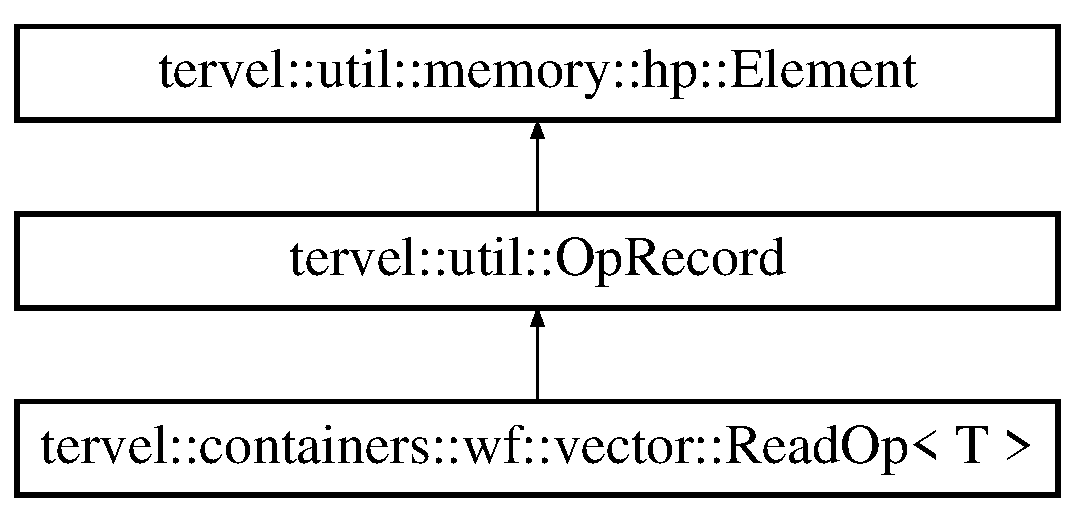
\includegraphics[height=3.000000cm]{classtervel_1_1containers_1_1wf_1_1vector_1_1_read_op}
\end{center}
\end{figure}
\subsection*{Public Member Functions}
\begin{DoxyCompactItemize}
\item 
\hyperlink{classtervel_1_1containers_1_1wf_1_1vector_1_1_read_op_ad0c7ce2b9563e63413925ae67a2cc0cc}{Read\+Op} (Vector$<$ T $>$ $\ast$vec, size\+\_\+t idx)
\item 
void \hyperlink{classtervel_1_1containers_1_1wf_1_1vector_1_1_read_op_ad2c5f63b0c39e1b30350656fcdd44538}{help\+\_\+complete} ()
\begin{DoxyCompactList}\small\item\em Implementations of this function that upon its return the operation described in the Op\+Record has been completed. \end{DoxyCompactList}\item 
bool \hyperlink{classtervel_1_1containers_1_1wf_1_1vector_1_1_read_op_af4e89911f2abe9ec130f5e03b1c98a50}{result} (T \&expected)
\end{DoxyCompactItemize}
\subsection*{Private Attributes}
\begin{DoxyCompactItemize}
\item 
Vector$<$ T $>$ $\ast$ \hyperlink{classtervel_1_1containers_1_1wf_1_1vector_1_1_read_op_aa345d1b47f36e47a74b185ea1ab11390}{vec\+\_\+}
\item 
size\+\_\+t \hyperlink{classtervel_1_1containers_1_1wf_1_1vector_1_1_read_op_ae16e934cbd5a237eb3f3c8dca70c4aa0}{idx\+\_\+}
\item 
std\+::atomic$<$ T $>$ \hyperlink{classtervel_1_1containers_1_1wf_1_1vector_1_1_read_op_accb5f2574e02c570e6fc7386e65d2ddf}{value\+\_\+} \{Vector$<$T$>$\+::c\+\_\+not\+\_\+value\+\_\+\}
\end{DoxyCompactItemize}
\subsection*{Static Private Attributes}
\begin{DoxyCompactItemize}
\item 
static const T \hyperlink{classtervel_1_1containers_1_1wf_1_1vector_1_1_read_op_a85fb04ba215b356679573518921879e0}{c\+\_\+fail\+\_\+value\+\_\+} \{static\+\_\+cast$<$T$>$($\sim$0x1\+L)\}
\end{DoxyCompactItemize}


\subsection{Constructor \& Destructor Documentation}
\hypertarget{classtervel_1_1containers_1_1wf_1_1vector_1_1_read_op_ad0c7ce2b9563e63413925ae67a2cc0cc}{}\index{tervel\+::containers\+::wf\+::vector\+::\+Read\+Op@{tervel\+::containers\+::wf\+::vector\+::\+Read\+Op}!Read\+Op@{Read\+Op}}
\index{Read\+Op@{Read\+Op}!tervel\+::containers\+::wf\+::vector\+::\+Read\+Op@{tervel\+::containers\+::wf\+::vector\+::\+Read\+Op}}
\subsubsection[{Read\+Op(\+Vector$<$ T $>$ $\ast$vec, size\+\_\+t idx)}]{\setlength{\rightskip}{0pt plus 5cm}template$<$typename T $>$ {\bf tervel\+::containers\+::wf\+::vector\+::\+Read\+Op}$<$ T $>$\+::{\bf Read\+Op} (
\begin{DoxyParamCaption}
\item[{Vector$<$ T $>$ $\ast$}]{vec, }
\item[{size\+\_\+t}]{idx}
\end{DoxyParamCaption}
)\hspace{0.3cm}{\ttfamily [inline]}}\label{classtervel_1_1containers_1_1wf_1_1vector_1_1_read_op_ad0c7ce2b9563e63413925ae67a2cc0cc}


\subsection{Member Function Documentation}
\hypertarget{classtervel_1_1containers_1_1wf_1_1vector_1_1_read_op_ad2c5f63b0c39e1b30350656fcdd44538}{}\index{tervel\+::containers\+::wf\+::vector\+::\+Read\+Op@{tervel\+::containers\+::wf\+::vector\+::\+Read\+Op}!help\+\_\+complete@{help\+\_\+complete}}
\index{help\+\_\+complete@{help\+\_\+complete}!tervel\+::containers\+::wf\+::vector\+::\+Read\+Op@{tervel\+::containers\+::wf\+::vector\+::\+Read\+Op}}
\subsubsection[{help\+\_\+complete()}]{\setlength{\rightskip}{0pt plus 5cm}template$<$typename T $>$ void {\bf tervel\+::containers\+::wf\+::vector\+::\+Read\+Op}$<$ T $>$\+::help\+\_\+complete (
\begin{DoxyParamCaption}
{}
\end{DoxyParamCaption}
)\hspace{0.3cm}{\ttfamily [inline]}, {\ttfamily [virtual]}}\label{classtervel_1_1containers_1_1wf_1_1vector_1_1_read_op_ad2c5f63b0c39e1b30350656fcdd44538}


Implementations of this function that upon its return the operation described in the Op\+Record has been completed. 

As such it must be thread-\/safe and the extending class must contain all the information necessary to complete the operation. 

Implements \hyperlink{classtervel_1_1util_1_1_op_record_aa75ab39688a8d4cceb6a1ef0409537c0}{tervel\+::util\+::\+Op\+Record}.

\hypertarget{classtervel_1_1containers_1_1wf_1_1vector_1_1_read_op_af4e89911f2abe9ec130f5e03b1c98a50}{}\index{tervel\+::containers\+::wf\+::vector\+::\+Read\+Op@{tervel\+::containers\+::wf\+::vector\+::\+Read\+Op}!result@{result}}
\index{result@{result}!tervel\+::containers\+::wf\+::vector\+::\+Read\+Op@{tervel\+::containers\+::wf\+::vector\+::\+Read\+Op}}
\subsubsection[{result(\+T \&expected)}]{\setlength{\rightskip}{0pt plus 5cm}template$<$typename T $>$ bool {\bf tervel\+::containers\+::wf\+::vector\+::\+Read\+Op}$<$ T $>$\+::result (
\begin{DoxyParamCaption}
\item[{T \&}]{expected}
\end{DoxyParamCaption}
)\hspace{0.3cm}{\ttfamily [inline]}}\label{classtervel_1_1containers_1_1wf_1_1vector_1_1_read_op_af4e89911f2abe9ec130f5e03b1c98a50}


\subsection{Member Data Documentation}
\hypertarget{classtervel_1_1containers_1_1wf_1_1vector_1_1_read_op_a85fb04ba215b356679573518921879e0}{}\index{tervel\+::containers\+::wf\+::vector\+::\+Read\+Op@{tervel\+::containers\+::wf\+::vector\+::\+Read\+Op}!c\+\_\+fail\+\_\+value\+\_\+@{c\+\_\+fail\+\_\+value\+\_\+}}
\index{c\+\_\+fail\+\_\+value\+\_\+@{c\+\_\+fail\+\_\+value\+\_\+}!tervel\+::containers\+::wf\+::vector\+::\+Read\+Op@{tervel\+::containers\+::wf\+::vector\+::\+Read\+Op}}
\subsubsection[{c\+\_\+fail\+\_\+value\+\_\+}]{\setlength{\rightskip}{0pt plus 5cm}template$<$typename T $>$ const T {\bf tervel\+::containers\+::wf\+::vector\+::\+Read\+Op}$<$ T $>$\+::c\+\_\+fail\+\_\+value\+\_\+ \{static\+\_\+cast$<$T$>$($\sim$0x1\+L)\}\hspace{0.3cm}{\ttfamily [static]}, {\ttfamily [private]}}\label{classtervel_1_1containers_1_1wf_1_1vector_1_1_read_op_a85fb04ba215b356679573518921879e0}
\hypertarget{classtervel_1_1containers_1_1wf_1_1vector_1_1_read_op_ae16e934cbd5a237eb3f3c8dca70c4aa0}{}\index{tervel\+::containers\+::wf\+::vector\+::\+Read\+Op@{tervel\+::containers\+::wf\+::vector\+::\+Read\+Op}!idx\+\_\+@{idx\+\_\+}}
\index{idx\+\_\+@{idx\+\_\+}!tervel\+::containers\+::wf\+::vector\+::\+Read\+Op@{tervel\+::containers\+::wf\+::vector\+::\+Read\+Op}}
\subsubsection[{idx\+\_\+}]{\setlength{\rightskip}{0pt plus 5cm}template$<$typename T $>$ size\+\_\+t {\bf tervel\+::containers\+::wf\+::vector\+::\+Read\+Op}$<$ T $>$\+::idx\+\_\+\hspace{0.3cm}{\ttfamily [private]}}\label{classtervel_1_1containers_1_1wf_1_1vector_1_1_read_op_ae16e934cbd5a237eb3f3c8dca70c4aa0}
\hypertarget{classtervel_1_1containers_1_1wf_1_1vector_1_1_read_op_accb5f2574e02c570e6fc7386e65d2ddf}{}\index{tervel\+::containers\+::wf\+::vector\+::\+Read\+Op@{tervel\+::containers\+::wf\+::vector\+::\+Read\+Op}!value\+\_\+@{value\+\_\+}}
\index{value\+\_\+@{value\+\_\+}!tervel\+::containers\+::wf\+::vector\+::\+Read\+Op@{tervel\+::containers\+::wf\+::vector\+::\+Read\+Op}}
\subsubsection[{value\+\_\+}]{\setlength{\rightskip}{0pt plus 5cm}template$<$typename T $>$ std\+::atomic$<$T$>$ {\bf tervel\+::containers\+::wf\+::vector\+::\+Read\+Op}$<$ T $>$\+::value\+\_\+ \{Vector$<$T$>$\+::c\+\_\+not\+\_\+value\+\_\+\}\hspace{0.3cm}{\ttfamily [private]}}\label{classtervel_1_1containers_1_1wf_1_1vector_1_1_read_op_accb5f2574e02c570e6fc7386e65d2ddf}
\hypertarget{classtervel_1_1containers_1_1wf_1_1vector_1_1_read_op_aa345d1b47f36e47a74b185ea1ab11390}{}\index{tervel\+::containers\+::wf\+::vector\+::\+Read\+Op@{tervel\+::containers\+::wf\+::vector\+::\+Read\+Op}!vec\+\_\+@{vec\+\_\+}}
\index{vec\+\_\+@{vec\+\_\+}!tervel\+::containers\+::wf\+::vector\+::\+Read\+Op@{tervel\+::containers\+::wf\+::vector\+::\+Read\+Op}}
\subsubsection[{vec\+\_\+}]{\setlength{\rightskip}{0pt plus 5cm}template$<$typename T $>$ Vector$<$T$>$$\ast$ {\bf tervel\+::containers\+::wf\+::vector\+::\+Read\+Op}$<$ T $>$\+::vec\+\_\+\hspace{0.3cm}{\ttfamily [private]}}\label{classtervel_1_1containers_1_1wf_1_1vector_1_1_read_op_aa345d1b47f36e47a74b185ea1ab11390}


The documentation for this class was generated from the following file\+:\begin{DoxyCompactItemize}
\item 
tervel/containers/wf/vector/\hyperlink{read__op_8h}{read\+\_\+op.\+h}\end{DoxyCompactItemize}

\hypertarget{classtervel_1_1util_1_1_recursive_action}{}\section{tervel\+:\+:util\+:\+:Recursive\+Action Class Reference}
\label{classtervel_1_1util_1_1_recursive_action}\index{tervel\+::util\+::\+Recursive\+Action@{tervel\+::util\+::\+Recursive\+Action}}


Helper class for R\+A\+I\+I management of recursive helping of threads.  




{\ttfamily \#include $<$recursive\+\_\+action.\+h$>$}

\subsection*{Public Member Functions}
\begin{DoxyCompactItemize}
\item 
\hyperlink{classtervel_1_1util_1_1_recursive_action_a9b933d52b081bc2bec138f44e035cfb4}{Recursive\+Action} ()
\item 
\hyperlink{classtervel_1_1util_1_1_recursive_action_aecf790a95c56d002498a74e7bf064ed4}{$\sim$\+Recursive\+Action} ()
\end{DoxyCompactItemize}
\subsection*{Static Public Member Functions}
\begin{DoxyCompactItemize}
\item 
static bool \hyperlink{classtervel_1_1util_1_1_recursive_action_a04517ab2addf5809dc3a3ac305043e59}{recursive\+\_\+return} (bool change=false, bool value=false)
\item 
static void \hyperlink{classtervel_1_1util_1_1_recursive_action_ad03949b4e1aad8fb562db5b3ea56633b}{set\+\_\+recursive\+\_\+return} ()
\item 
static void \hyperlink{classtervel_1_1util_1_1_recursive_action_aff53861114a7b16bad441839a1247f6f}{clear\+\_\+recursive\+\_\+return} ()
\item 
static size\+\_\+t \hyperlink{classtervel_1_1util_1_1_recursive_action_a003b6df6a071e6299e27ac16f8d0c8f2}{recursive\+\_\+depth} (size\+\_\+t i=0)
\begin{DoxyCompactList}\small\item\em Adds the passed value and returns the pre-\/incremented value. \end{DoxyCompactList}\end{DoxyCompactItemize}
\subsection*{Private Member Functions}
\begin{DoxyCompactItemize}
\item 
\hyperlink{classtervel_1_1util_1_1_recursive_action_a309845abdb6e9dbbb31568c81257ed86}{D\+I\+S\+A\+L\+L\+O\+W\+\_\+\+C\+O\+P\+Y\+\_\+\+A\+N\+D\+\_\+\+A\+S\+S\+I\+G\+N} (\hyperlink{classtervel_1_1util_1_1_recursive_action}{Recursive\+Action})
\end{DoxyCompactItemize}


\subsection{Detailed Description}
Helper class for R\+A\+I\+I management of recursive helping of threads. 

Lifetime of this object handles the increment and decrement of the {\ttfamily recursive\+\_\+depth} of the given Thread\+Info object and sets the {\ttfamily recursive\+\_\+return} if needed. 

\subsection{Constructor \& Destructor Documentation}
\hypertarget{classtervel_1_1util_1_1_recursive_action_a9b933d52b081bc2bec138f44e035cfb4}{}\index{tervel\+::util\+::\+Recursive\+Action@{tervel\+::util\+::\+Recursive\+Action}!Recursive\+Action@{Recursive\+Action}}
\index{Recursive\+Action@{Recursive\+Action}!tervel\+::util\+::\+Recursive\+Action@{tervel\+::util\+::\+Recursive\+Action}}
\subsubsection[{Recursive\+Action()}]{\setlength{\rightskip}{0pt plus 5cm}tervel\+::util\+::\+Recursive\+Action\+::\+Recursive\+Action (
\begin{DoxyParamCaption}
{}
\end{DoxyParamCaption}
)\hspace{0.3cm}{\ttfamily [inline]}}\label{classtervel_1_1util_1_1_recursive_action_a9b933d52b081bc2bec138f44e035cfb4}
\hypertarget{classtervel_1_1util_1_1_recursive_action_aecf790a95c56d002498a74e7bf064ed4}{}\index{tervel\+::util\+::\+Recursive\+Action@{tervel\+::util\+::\+Recursive\+Action}!````~Recursive\+Action@{$\sim$\+Recursive\+Action}}
\index{````~Recursive\+Action@{$\sim$\+Recursive\+Action}!tervel\+::util\+::\+Recursive\+Action@{tervel\+::util\+::\+Recursive\+Action}}
\subsubsection[{$\sim$\+Recursive\+Action()}]{\setlength{\rightskip}{0pt plus 5cm}tervel\+::util\+::\+Recursive\+Action\+::$\sim$\+Recursive\+Action (
\begin{DoxyParamCaption}
{}
\end{DoxyParamCaption}
)\hspace{0.3cm}{\ttfamily [inline]}}\label{classtervel_1_1util_1_1_recursive_action_aecf790a95c56d002498a74e7bf064ed4}


\subsection{Member Function Documentation}
\hypertarget{classtervel_1_1util_1_1_recursive_action_aff53861114a7b16bad441839a1247f6f}{}\index{tervel\+::util\+::\+Recursive\+Action@{tervel\+::util\+::\+Recursive\+Action}!clear\+\_\+recursive\+\_\+return@{clear\+\_\+recursive\+\_\+return}}
\index{clear\+\_\+recursive\+\_\+return@{clear\+\_\+recursive\+\_\+return}!tervel\+::util\+::\+Recursive\+Action@{tervel\+::util\+::\+Recursive\+Action}}
\subsubsection[{clear\+\_\+recursive\+\_\+return()}]{\setlength{\rightskip}{0pt plus 5cm}static void tervel\+::util\+::\+Recursive\+Action\+::clear\+\_\+recursive\+\_\+return (
\begin{DoxyParamCaption}
{}
\end{DoxyParamCaption}
)\hspace{0.3cm}{\ttfamily [inline]}, {\ttfamily [static]}}\label{classtervel_1_1util_1_1_recursive_action_aff53861114a7b16bad441839a1247f6f}
\hypertarget{classtervel_1_1util_1_1_recursive_action_a309845abdb6e9dbbb31568c81257ed86}{}\index{tervel\+::util\+::\+Recursive\+Action@{tervel\+::util\+::\+Recursive\+Action}!D\+I\+S\+A\+L\+L\+O\+W\+\_\+\+C\+O\+P\+Y\+\_\+\+A\+N\+D\+\_\+\+A\+S\+S\+I\+G\+N@{D\+I\+S\+A\+L\+L\+O\+W\+\_\+\+C\+O\+P\+Y\+\_\+\+A\+N\+D\+\_\+\+A\+S\+S\+I\+G\+N}}
\index{D\+I\+S\+A\+L\+L\+O\+W\+\_\+\+C\+O\+P\+Y\+\_\+\+A\+N\+D\+\_\+\+A\+S\+S\+I\+G\+N@{D\+I\+S\+A\+L\+L\+O\+W\+\_\+\+C\+O\+P\+Y\+\_\+\+A\+N\+D\+\_\+\+A\+S\+S\+I\+G\+N}!tervel\+::util\+::\+Recursive\+Action@{tervel\+::util\+::\+Recursive\+Action}}
\subsubsection[{D\+I\+S\+A\+L\+L\+O\+W\+\_\+\+C\+O\+P\+Y\+\_\+\+A\+N\+D\+\_\+\+A\+S\+S\+I\+G\+N(\+Recursive\+Action)}]{\setlength{\rightskip}{0pt plus 5cm}tervel\+::util\+::\+Recursive\+Action\+::\+D\+I\+S\+A\+L\+L\+O\+W\+\_\+\+C\+O\+P\+Y\+\_\+\+A\+N\+D\+\_\+\+A\+S\+S\+I\+G\+N (
\begin{DoxyParamCaption}
\item[{{\bf Recursive\+Action}}]{}
\end{DoxyParamCaption}
)\hspace{0.3cm}{\ttfamily [private]}}\label{classtervel_1_1util_1_1_recursive_action_a309845abdb6e9dbbb31568c81257ed86}
\hypertarget{classtervel_1_1util_1_1_recursive_action_a003b6df6a071e6299e27ac16f8d0c8f2}{}\index{tervel\+::util\+::\+Recursive\+Action@{tervel\+::util\+::\+Recursive\+Action}!recursive\+\_\+depth@{recursive\+\_\+depth}}
\index{recursive\+\_\+depth@{recursive\+\_\+depth}!tervel\+::util\+::\+Recursive\+Action@{tervel\+::util\+::\+Recursive\+Action}}
\subsubsection[{recursive\+\_\+depth(size\+\_\+t i=0)}]{\setlength{\rightskip}{0pt plus 5cm}static size\+\_\+t tervel\+::util\+::\+Recursive\+Action\+::recursive\+\_\+depth (
\begin{DoxyParamCaption}
\item[{size\+\_\+t}]{i = {\ttfamily 0}}
\end{DoxyParamCaption}
)\hspace{0.3cm}{\ttfamily [static]}}\label{classtervel_1_1util_1_1_recursive_action_a003b6df6a071e6299e27ac16f8d0c8f2}


Adds the passed value and returns the pre-\/incremented value. 


\begin{DoxyParams}{Parameters}
{\em i} & value to increment by \\
\hline
\end{DoxyParams}
\begin{DoxyReturn}{Returns}
the value before the increment 
\end{DoxyReturn}
\hypertarget{classtervel_1_1util_1_1_recursive_action_a04517ab2addf5809dc3a3ac305043e59}{}\index{tervel\+::util\+::\+Recursive\+Action@{tervel\+::util\+::\+Recursive\+Action}!recursive\+\_\+return@{recursive\+\_\+return}}
\index{recursive\+\_\+return@{recursive\+\_\+return}!tervel\+::util\+::\+Recursive\+Action@{tervel\+::util\+::\+Recursive\+Action}}
\subsubsection[{recursive\+\_\+return(bool change=false, bool value=false)}]{\setlength{\rightskip}{0pt plus 5cm}static bool tervel\+::util\+::\+Recursive\+Action\+::recursive\+\_\+return (
\begin{DoxyParamCaption}
\item[{bool}]{change = {\ttfamily false}, }
\item[{bool}]{value = {\ttfamily false}}
\end{DoxyParamCaption}
)\hspace{0.3cm}{\ttfamily [static]}}\label{classtervel_1_1util_1_1_recursive_action_a04517ab2addf5809dc3a3ac305043e59}
\begin{DoxyReturn}{Returns}
whether or not the thread is performing a recursive return. 
\end{DoxyReturn}
\hypertarget{classtervel_1_1util_1_1_recursive_action_ad03949b4e1aad8fb562db5b3ea56633b}{}\index{tervel\+::util\+::\+Recursive\+Action@{tervel\+::util\+::\+Recursive\+Action}!set\+\_\+recursive\+\_\+return@{set\+\_\+recursive\+\_\+return}}
\index{set\+\_\+recursive\+\_\+return@{set\+\_\+recursive\+\_\+return}!tervel\+::util\+::\+Recursive\+Action@{tervel\+::util\+::\+Recursive\+Action}}
\subsubsection[{set\+\_\+recursive\+\_\+return()}]{\setlength{\rightskip}{0pt plus 5cm}static void tervel\+::util\+::\+Recursive\+Action\+::set\+\_\+recursive\+\_\+return (
\begin{DoxyParamCaption}
{}
\end{DoxyParamCaption}
)\hspace{0.3cm}{\ttfamily [inline]}, {\ttfamily [static]}}\label{classtervel_1_1util_1_1_recursive_action_ad03949b4e1aad8fb562db5b3ea56633b}


The documentation for this class was generated from the following file\+:\begin{DoxyCompactItemize}
\item 
tervel/util/\hyperlink{recursive__action_8h}{recursive\+\_\+action.\+h}\end{DoxyCompactItemize}

\hypertarget{classtervel_1_1containers_1_1wf_1_1_ring_buffer}{}\section{tervel\+:\+:containers\+:\+:wf\+:\+:Ring\+Buffer$<$ T $>$ Class Template Reference}
\label{classtervel_1_1containers_1_1wf_1_1_ring_buffer}\index{tervel\+::containers\+::wf\+::\+Ring\+Buffer$<$ T $>$@{tervel\+::containers\+::wf\+::\+Ring\+Buffer$<$ T $>$}}


This is a non-\/blocking F\+I\+F\+O ring buffer design that was made wait-\/free by applying a progress assurance framework to it.  




{\ttfamily \#include $<$ring\+\_\+buffer.\+h$>$}

\subsection*{Classes}
\begin{DoxyCompactItemize}
\item 
class \hyperlink{classtervel_1_1containers_1_1wf_1_1_ring_buffer_1_1_buffer_op}{Buffer\+Op}
\item 
class \hyperlink{classtervel_1_1containers_1_1wf_1_1_ring_buffer_1_1_dequeue_op}{Dequeue\+Op}
\item 
class \hyperlink{classtervel_1_1containers_1_1wf_1_1_ring_buffer_1_1_enqueue_op}{Enqueue\+Op}
\item 
class \hyperlink{classtervel_1_1containers_1_1wf_1_1_ring_buffer_1_1_helper}{Helper}
\item 
class \hyperlink{classtervel_1_1containers_1_1wf_1_1_ring_buffer_1_1_value}{Value}
\begin{DoxyCompactList}\small\item\em \hyperlink{classtervel_1_1containers_1_1wf_1_1_ring_buffer}{Ring\+Buffer} value class, values stored in the class must extend it. \end{DoxyCompactList}\end{DoxyCompactItemize}
\subsection*{Public Member Functions}
\begin{DoxyCompactItemize}
\item 
\hyperlink{classtervel_1_1containers_1_1wf_1_1_ring_buffer_aa273f827eb69a6d148d1a3449d8a18ec}{Ring\+Buffer} (size\+\_\+t capacity)
\begin{DoxyCompactList}\small\item\em Ring Buffer constructor. \end{DoxyCompactList}\item 
bool \hyperlink{classtervel_1_1containers_1_1wf_1_1_ring_buffer_a7079b1f92598181c4ef7c179d1eb2773}{is\+Full} ()
\begin{DoxyCompactList}\small\item\em Returns whether or not the ring buffer is full. \end{DoxyCompactList}\item 
bool \hyperlink{classtervel_1_1containers_1_1wf_1_1_ring_buffer_a5af5dec4a0f9b17f419189352ff94826}{is\+Full} (int64\+\_\+t tail, int64\+\_\+t head)
\begin{DoxyCompactList}\small\item\em Returns whether or not the ring buffer is full. \end{DoxyCompactList}\item 
bool \hyperlink{classtervel_1_1containers_1_1wf_1_1_ring_buffer_a4e01d955bd0bc4b75ad1e79fe5c3b1c7}{is\+Empty} ()
\begin{DoxyCompactList}\small\item\em Returns whether or not the ring buffer is empty. \end{DoxyCompactList}\item 
bool \hyperlink{classtervel_1_1containers_1_1wf_1_1_ring_buffer_a537c3fd338a5d277f7d20d8ca52c96ac}{is\+Empty} (int64\+\_\+t tail, int64\+\_\+t head)
\begin{DoxyCompactList}\small\item\em Returns whether or not the ring buffer is empty. \end{DoxyCompactList}\item 
bool \hyperlink{classtervel_1_1containers_1_1wf_1_1_ring_buffer_a9a077f004d6e7844d21fbe6ca9c259e9}{enqueue} (T value)
\begin{DoxyCompactList}\small\item\em Enqueues the passed value into the buffer. \end{DoxyCompactList}\item 
bool \hyperlink{classtervel_1_1containers_1_1wf_1_1_ring_buffer_a54ca61cd44983b793173eadca794f64a}{dequeue} (T \&value)
\begin{DoxyCompactList}\small\item\em Dequeues a value from the buffer. \end{DoxyCompactList}\item 
std\+::string \hyperlink{classtervel_1_1containers_1_1wf_1_1_ring_buffer_a461e01d08e025fe89c64e900a219e953}{debug\+\_\+string} ()
\begin{DoxyCompactList}\small\item\em This function returns a string debugging information. \end{DoxyCompactList}\end{DoxyCompactItemize}
\subsection*{Private Member Functions}
\begin{DoxyCompactItemize}
\item 
bool \hyperlink{classtervel_1_1containers_1_1wf_1_1_ring_buffer_a7e82ecdcd6145daf90c8d49d04fd270d}{read\+Value} (int64\+\_\+t pos, uintptr\+\_\+t \&val)
\begin{DoxyCompactList}\small\item\em This function attempts to load a value from the buffer. \end{DoxyCompactList}\item 
void \hyperlink{classtervel_1_1containers_1_1wf_1_1_ring_buffer_a6f9c4dfd96a9b4c7c5aab52174171eb5}{get\+Info} (uintptr\+\_\+t val, int64\+\_\+t \&val\+\_\+seqid, bool \&val\+\_\+is\+Value\+Type, bool \&val\+\_\+is\+Marked)
\begin{DoxyCompactList}\small\item\em This function is used to get information from a value read from the ring buffer. \end{DoxyCompactList}\item 
int64\+\_\+t \hyperlink{classtervel_1_1containers_1_1wf_1_1_ring_buffer_a20683c75c286a8a22e97cbcbe5b8c787}{next\+Head} ()
\begin{DoxyCompactList}\small\item\em performs a fetch-\/and-\/add on the head counter \end{DoxyCompactList}\item 
int64\+\_\+t \hyperlink{classtervel_1_1containers_1_1wf_1_1_ring_buffer_a5f45b94d3225418fdec729f483db8c7c}{get\+Head} ()
\begin{DoxyCompactList}\small\item\em performs an atomic load on the head counter \end{DoxyCompactList}\item 
int64\+\_\+t \hyperlink{classtervel_1_1containers_1_1wf_1_1_ring_buffer_ae6ebc11d1ba6f884067ddc5b0b4e411f}{cas\+Head} (int64\+\_\+t \&expected, int64\+\_\+t new\+\_\+val)
\item 
int64\+\_\+t \hyperlink{classtervel_1_1containers_1_1wf_1_1_ring_buffer_a2b6cdb8a410b919e6aed90d130e3d4fa}{next\+Tail} ()
\begin{DoxyCompactList}\small\item\em performs a fetch-\/and-\/add on the tail counter \end{DoxyCompactList}\item 
int64\+\_\+t \hyperlink{classtervel_1_1containers_1_1wf_1_1_ring_buffer_ab757ccb32546ad168ff70295e53bb509}{get\+Tail} ()
\begin{DoxyCompactList}\small\item\em performs an atomic load on the tail counter \end{DoxyCompactList}\item 
int64\+\_\+t \hyperlink{classtervel_1_1containers_1_1wf_1_1_ring_buffer_a9c808379ab96e7d55d23168530ff4505}{cas\+Tail} (int64\+\_\+t \&expected, int64\+\_\+t new\+\_\+val)
\item 
int64\+\_\+t \hyperlink{classtervel_1_1containers_1_1wf_1_1_ring_buffer_aca988376ab980bce614ddbe0c279af73}{next\+Seq\+Id} (int64\+\_\+t seqid)
\begin{DoxyCompactList}\small\item\em Returns the next seqid. \end{DoxyCompactList}\item 
int64\+\_\+t \hyperlink{classtervel_1_1containers_1_1wf_1_1_ring_buffer_a909965b7e584d94ceedec35f5d06399e}{get\+Pos} (int64\+\_\+t seqid)
\begin{DoxyCompactList}\small\item\em Returns the position a seqid belongs at. \end{DoxyCompactList}\item 
bool \hyperlink{classtervel_1_1containers_1_1wf_1_1_ring_buffer_a54a5d1b842d3a70708d64460948628bd}{backoff} (int64\+\_\+t pos, uintptr\+\_\+t val)
\begin{DoxyCompactList}\small\item\em A backoff routine in the event of thread delay. \end{DoxyCompactList}\item 
void \hyperlink{classtervel_1_1containers_1_1wf_1_1_ring_buffer_aed86f62144a5709a09273cfd9b64d28a}{atomic\+\_\+delay\+\_\+mark} (int64\+\_\+t pos)
\begin{DoxyCompactList}\small\item\em This function places a bitmark on the value held at address. \end{DoxyCompactList}\item 
std\+::string \hyperlink{classtervel_1_1containers_1_1wf_1_1_ring_buffer_a2ea530f34dec3354636c48c28066b320}{debug\+\_\+string} (uintptr\+\_\+t val)
\begin{DoxyCompactList}\small\item\em This prints out debugging information. \end{DoxyCompactList}\end{DoxyCompactItemize}
\subsection*{Static Private Member Functions}
\begin{DoxyCompactItemize}
\item 
static uintptr\+\_\+t \hyperlink{classtervel_1_1containers_1_1wf_1_1_ring_buffer_ad29913ad7598a2825cd76200eef0f296}{Empty\+Type} (int64\+\_\+t seqid)
\begin{DoxyCompactList}\small\item\em Creates a uintptr\+\_\+t that represents an Empty\+Type. \end{DoxyCompactList}\item 
static int64\+\_\+t \hyperlink{classtervel_1_1containers_1_1wf_1_1_ring_buffer_ad28c5560eec05806c2a6c2c9d49b51df}{get\+Empty\+Type\+Seq\+Id} (uintptr\+\_\+t val)
\begin{DoxyCompactList}\small\item\em Returns the seqid encoded in the passed value. \end{DoxyCompactList}\item 
static uintptr\+\_\+t \hyperlink{classtervel_1_1containers_1_1wf_1_1_ring_buffer_a6d65a8409987f61a0fe48193b9073578}{Value\+Type} (T value, int64\+\_\+t seqid)
\begin{DoxyCompactList}\small\item\em Creates a uintptr\+\_\+t that represents an Value\+Type. \end{DoxyCompactList}\item 
static T \hyperlink{classtervel_1_1containers_1_1wf_1_1_ring_buffer_a1f068a3e3fb8afd732fb24629f9af573}{get\+Value\+Type} (uintptr\+\_\+t val)
\begin{DoxyCompactList}\small\item\em Returns the value type from a uintptr. \end{DoxyCompactList}\item 
static int64\+\_\+t \hyperlink{classtervel_1_1containers_1_1wf_1_1_ring_buffer_afcb8d6559b878ea259ad0d0c03260ce5}{get\+Value\+Type\+Seq\+Id} (uintptr\+\_\+t val)
\begin{DoxyCompactList}\small\item\em Returns the seqid of the passed value. \end{DoxyCompactList}\item 
static uintptr\+\_\+t \hyperlink{classtervel_1_1containers_1_1wf_1_1_ring_buffer_a82ae33c04b67eec192d19ec0e652012f}{Delay\+Mark\+Value} (uintptr\+\_\+t val)
\begin{DoxyCompactList}\small\item\em Takes a uintptr\+\_\+t and places a bitmark on the delay\+Mark\+\_\+lsb. \end{DoxyCompactList}\item 
static bool \hyperlink{classtervel_1_1containers_1_1wf_1_1_ring_buffer_afa26a1ffab8e479f7c8158789d05a2ed}{is\+Empty\+Type} (uintptr\+\_\+t p)
\begin{DoxyCompactList}\small\item\em returns whether or not p represents an Empty\+Type \end{DoxyCompactList}\item 
static bool \hyperlink{classtervel_1_1containers_1_1wf_1_1_ring_buffer_aa6254103b63556a143f568a23a189193}{is\+Value\+Type} (uintptr\+\_\+t p)
\begin{DoxyCompactList}\small\item\em returns whether or not p represents an Value\+Type \end{DoxyCompactList}\item 
static bool \hyperlink{classtervel_1_1containers_1_1wf_1_1_ring_buffer_ac0d773c57b2c0718e1308cbc5726f0a8}{is\+Delayed\+Marked} (uintptr\+\_\+t p)
\begin{DoxyCompactList}\small\item\em returns whether or not p has a delay mark \end{DoxyCompactList}\item 
static int64\+\_\+t \hyperlink{classtervel_1_1containers_1_1wf_1_1_ring_buffer_ae432cff608036acb82351fb37df2201e}{counter\+Action} (std\+::atomic$<$ int64\+\_\+t $>$ \&counter, int64\+\_\+t val)
\begin{DoxyCompactList}\small\item\em utility function for incrementing counter \end{DoxyCompactList}\end{DoxyCompactItemize}
\subsection*{Private Attributes}
\begin{DoxyCompactItemize}
\item 
const int64\+\_\+t \hyperlink{classtervel_1_1containers_1_1wf_1_1_ring_buffer_a41e3b8510f4ffd470709fe8e83868933}{capacity\+\_\+}
\item 
std\+::atomic$<$ int64\+\_\+t $>$ \hyperlink{classtervel_1_1containers_1_1wf_1_1_ring_buffer_a94a7b260355e3e1c3c97b649304b3302}{head\+\_\+} \{0\}
\item 
std\+::atomic$<$ int64\+\_\+t $>$ \hyperlink{classtervel_1_1containers_1_1wf_1_1_ring_buffer_acd823ce60f711bf6ea20799992844183}{tail\+\_\+} \{0\}
\item 
std\+::unique\+\_\+ptr$<$ std\+::atomic$<$ uintptr\+\_\+t $>$\mbox{[}$\,$\mbox{]}$>$ \hyperlink{classtervel_1_1containers_1_1wf_1_1_ring_buffer_a609506aa3f330fcf9ada6ca622514bd5}{array\+\_\+}
\end{DoxyCompactItemize}
\subsection*{Static Private Attributes}
\begin{DoxyCompactItemize}
\item 
static const uintptr\+\_\+t \hyperlink{classtervel_1_1containers_1_1wf_1_1_ring_buffer_a88443e08c1d248ce79ed7a2dc54c00c4}{num\+\_\+lsb} = 3
\item 
static const uintptr\+\_\+t \hyperlink{classtervel_1_1containers_1_1wf_1_1_ring_buffer_a1bd646f1d7df0a14d64078d2dcef1cb5}{delay\+Mark\+\_\+lsb} = 0x1
\item 
static const uintptr\+\_\+t \hyperlink{classtervel_1_1containers_1_1wf_1_1_ring_buffer_aaeeec7e2573a54c06823fb6800437b4f}{emptytype\+\_\+lsb} = 0x2
\item 
static const uintptr\+\_\+t \hyperlink{classtervel_1_1containers_1_1wf_1_1_ring_buffer_a83e184f9dffd2a06038726f74640c554}{oprec\+\_\+lsb} = 0x4
\item 
static const uintptr\+\_\+t \hyperlink{classtervel_1_1containers_1_1wf_1_1_ring_buffer_afabc2215759bfbb00144024609700b7d}{clear\+\_\+lsb} = 7
\end{DoxyCompactItemize}


\subsection{Detailed Description}
\subsubsection*{template$<$typename T$>$class tervel\+::containers\+::wf\+::\+Ring\+Buffer$<$ T $>$}

This is a non-\/blocking F\+I\+F\+O ring buffer design that was made wait-\/free by applying a progress assurance framework to it. 

If is\+Delayed never returns true then it will not use additional memory. However, if it does, then it will allocate some objects which are protected by hazard pointer protection.

This ring buffer is implemented on a statically sized array. It can only store pointer sized objects that extend the \hyperlink{classtervel_1_1containers_1_1wf_1_1_ring_buffer_1_1_value}{Value} class. Further it reserves the 3 L\+S\+B for type identification, which makes it compatible only with 64 bit systems

It supports enqueue, dequeue, is\+Full, and is\+Empty operations


\begin{DoxyTemplParams}{Template Parameters}
{\em T} & The type of information stored, must be a pointer and the class must extend \hyperlink{classtervel_1_1containers_1_1wf_1_1_ring_buffer_1_1_value}{Ring\+Buffer\+::\+Value}. \\
\hline
\end{DoxyTemplParams}


\subsection{Constructor \& Destructor Documentation}
\hypertarget{classtervel_1_1containers_1_1wf_1_1_ring_buffer_aa273f827eb69a6d148d1a3449d8a18ec}{}\index{tervel\+::containers\+::wf\+::\+Ring\+Buffer@{tervel\+::containers\+::wf\+::\+Ring\+Buffer}!Ring\+Buffer@{Ring\+Buffer}}
\index{Ring\+Buffer@{Ring\+Buffer}!tervel\+::containers\+::wf\+::\+Ring\+Buffer@{tervel\+::containers\+::wf\+::\+Ring\+Buffer}}
\subsubsection[{Ring\+Buffer(size\+\_\+t capacity)}]{\setlength{\rightskip}{0pt plus 5cm}template$<$typename T $>$ {\bf tervel\+::containers\+::wf\+::\+Ring\+Buffer}$<$ T $>$\+::{\bf Ring\+Buffer} (
\begin{DoxyParamCaption}
\item[{size\+\_\+t}]{capacity}
\end{DoxyParamCaption}
)}\label{classtervel_1_1containers_1_1wf_1_1_ring_buffer_aa273f827eb69a6d148d1a3449d8a18ec}


Ring Buffer constructor. 

This constructs and initializes the ring buffer object


\begin{DoxyParams}{Parameters}
{\em capacity} & the length of the internal array to allocate. \\
\hline
\end{DoxyParams}


\subsection{Member Function Documentation}
\hypertarget{classtervel_1_1containers_1_1wf_1_1_ring_buffer_aed86f62144a5709a09273cfd9b64d28a}{}\index{tervel\+::containers\+::wf\+::\+Ring\+Buffer@{tervel\+::containers\+::wf\+::\+Ring\+Buffer}!atomic\+\_\+delay\+\_\+mark@{atomic\+\_\+delay\+\_\+mark}}
\index{atomic\+\_\+delay\+\_\+mark@{atomic\+\_\+delay\+\_\+mark}!tervel\+::containers\+::wf\+::\+Ring\+Buffer@{tervel\+::containers\+::wf\+::\+Ring\+Buffer}}
\subsubsection[{atomic\+\_\+delay\+\_\+mark(int64\+\_\+t pos)}]{\setlength{\rightskip}{0pt plus 5cm}template$<$typename T $>$ void {\bf tervel\+::containers\+::wf\+::\+Ring\+Buffer}$<$ T $>$\+::atomic\+\_\+delay\+\_\+mark (
\begin{DoxyParamCaption}
\item[{int64\+\_\+t}]{pos}
\end{DoxyParamCaption}
)\hspace{0.3cm}{\ttfamily [private]}}\label{classtervel_1_1containers_1_1wf_1_1_ring_buffer_aed86f62144a5709a09273cfd9b64d28a}


This function places a bitmark on the value held at address. 

This function places a bitmark on the value held at address by calling address-\/$>$fetch\+\_\+or(delay\+Mark\+\_\+lsb) and then it loads the new current value and assigns it to val.


\begin{DoxyParams}{Parameters}
{\em pos} & The position to perform the blind bitmark. \\
\hline
\end{DoxyParams}
\hypertarget{classtervel_1_1containers_1_1wf_1_1_ring_buffer_a54a5d1b842d3a70708d64460948628bd}{}\index{tervel\+::containers\+::wf\+::\+Ring\+Buffer@{tervel\+::containers\+::wf\+::\+Ring\+Buffer}!backoff@{backoff}}
\index{backoff@{backoff}!tervel\+::containers\+::wf\+::\+Ring\+Buffer@{tervel\+::containers\+::wf\+::\+Ring\+Buffer}}
\subsubsection[{backoff(int64\+\_\+t pos, uintptr\+\_\+t val)}]{\setlength{\rightskip}{0pt plus 5cm}template$<$typename T $>$ bool {\bf tervel\+::containers\+::wf\+::\+Ring\+Buffer}$<$ T $>$\+::backoff (
\begin{DoxyParamCaption}
\item[{int64\+\_\+t}]{pos, }
\item[{uintptr\+\_\+t}]{val}
\end{DoxyParamCaption}
)\hspace{0.3cm}{\ttfamily [private]}}\label{classtervel_1_1containers_1_1wf_1_1_ring_buffer_a54a5d1b842d3a70708d64460948628bd}


A backoff routine in the event of thread delay. 

This function is called in the event the value at position on the ringbuffer is lagging behind as a result of a delayed thread.

It calls \hyperlink{namespacetervel_1_1util_a4505d4510f91a5cb1a766dea247f835f}{tervel\+::util\+::backoff()} and upon its return checks whether or the value at address has changed. If it has, it returns true, Else it returns false. If the value has changed the new value is assigned to val


\begin{DoxyParams}{Parameters}
{\em pos} & The pos val was read from \\
\hline
{\em val} & The last read value from address.\\
\hline
\end{DoxyParams}
\begin{DoxyReturn}{Returns}
whether or not the val changed. 
\end{DoxyReturn}
\hypertarget{classtervel_1_1containers_1_1wf_1_1_ring_buffer_ae6ebc11d1ba6f884067ddc5b0b4e411f}{}\index{tervel\+::containers\+::wf\+::\+Ring\+Buffer@{tervel\+::containers\+::wf\+::\+Ring\+Buffer}!cas\+Head@{cas\+Head}}
\index{cas\+Head@{cas\+Head}!tervel\+::containers\+::wf\+::\+Ring\+Buffer@{tervel\+::containers\+::wf\+::\+Ring\+Buffer}}
\subsubsection[{cas\+Head(int64\+\_\+t \&expected, int64\+\_\+t new\+\_\+val)}]{\setlength{\rightskip}{0pt plus 5cm}template$<$typename T $>$ int64\+\_\+t {\bf tervel\+::containers\+::wf\+::\+Ring\+Buffer}$<$ T $>$\+::cas\+Head (
\begin{DoxyParamCaption}
\item[{int64\+\_\+t \&}]{expected, }
\item[{int64\+\_\+t}]{new\+\_\+val}
\end{DoxyParamCaption}
)\hspace{0.3cm}{\ttfamily [private]}}\label{classtervel_1_1containers_1_1wf_1_1_ring_buffer_ae6ebc11d1ba6f884067ddc5b0b4e411f}
\hypertarget{classtervel_1_1containers_1_1wf_1_1_ring_buffer_a9c808379ab96e7d55d23168530ff4505}{}\index{tervel\+::containers\+::wf\+::\+Ring\+Buffer@{tervel\+::containers\+::wf\+::\+Ring\+Buffer}!cas\+Tail@{cas\+Tail}}
\index{cas\+Tail@{cas\+Tail}!tervel\+::containers\+::wf\+::\+Ring\+Buffer@{tervel\+::containers\+::wf\+::\+Ring\+Buffer}}
\subsubsection[{cas\+Tail(int64\+\_\+t \&expected, int64\+\_\+t new\+\_\+val)}]{\setlength{\rightskip}{0pt plus 5cm}template$<$typename T $>$ int64\+\_\+t {\bf tervel\+::containers\+::wf\+::\+Ring\+Buffer}$<$ T $>$\+::cas\+Tail (
\begin{DoxyParamCaption}
\item[{int64\+\_\+t \&}]{expected, }
\item[{int64\+\_\+t}]{new\+\_\+val}
\end{DoxyParamCaption}
)\hspace{0.3cm}{\ttfamily [private]}}\label{classtervel_1_1containers_1_1wf_1_1_ring_buffer_a9c808379ab96e7d55d23168530ff4505}
\hypertarget{classtervel_1_1containers_1_1wf_1_1_ring_buffer_ae432cff608036acb82351fb37df2201e}{}\index{tervel\+::containers\+::wf\+::\+Ring\+Buffer@{tervel\+::containers\+::wf\+::\+Ring\+Buffer}!counter\+Action@{counter\+Action}}
\index{counter\+Action@{counter\+Action}!tervel\+::containers\+::wf\+::\+Ring\+Buffer@{tervel\+::containers\+::wf\+::\+Ring\+Buffer}}
\subsubsection[{counter\+Action(std\+::atomic$<$ int64\+\_\+t $>$ \&counter, int64\+\_\+t val)}]{\setlength{\rightskip}{0pt plus 5cm}template$<$typename T $>$ int64\+\_\+t {\bf tervel\+::containers\+::wf\+::\+Ring\+Buffer}$<$ T $>$\+::counter\+Action (
\begin{DoxyParamCaption}
\item[{std\+::atomic$<$ int64\+\_\+t $>$ \&}]{counter, }
\item[{int64\+\_\+t}]{val}
\end{DoxyParamCaption}
)\hspace{0.3cm}{\ttfamily [inline]}, {\ttfamily [static]}, {\ttfamily [private]}}\label{classtervel_1_1containers_1_1wf_1_1_ring_buffer_ae432cff608036acb82351fb37df2201e}


utility function for incrementing counter 

contains internal checks on the returned value


\begin{DoxyParams}{Parameters}
{\em counter} & counter to increment \\
\hline
{\em val} & value by which to increment the counter\\
\hline
\end{DoxyParams}
\begin{DoxyReturn}{Returns}
returns the pre-\/incremented value of the tail counter. 
\end{DoxyReturn}
\hypertarget{classtervel_1_1containers_1_1wf_1_1_ring_buffer_a461e01d08e025fe89c64e900a219e953}{}\index{tervel\+::containers\+::wf\+::\+Ring\+Buffer@{tervel\+::containers\+::wf\+::\+Ring\+Buffer}!debug\+\_\+string@{debug\+\_\+string}}
\index{debug\+\_\+string@{debug\+\_\+string}!tervel\+::containers\+::wf\+::\+Ring\+Buffer@{tervel\+::containers\+::wf\+::\+Ring\+Buffer}}
\subsubsection[{debug\+\_\+string()}]{\setlength{\rightskip}{0pt plus 5cm}template$<$typename T $>$ std\+::string {\bf tervel\+::containers\+::wf\+::\+Ring\+Buffer}$<$ T $>$\+::debug\+\_\+string (
\begin{DoxyParamCaption}
{}
\end{DoxyParamCaption}
)}\label{classtervel_1_1containers_1_1wf_1_1_ring_buffer_a461e01d08e025fe89c64e900a219e953}


This function returns a string debugging information. 

This information includes \hyperlink{classtervel_1_1containers_1_1wf_1_1_ring_buffer_1_1_value}{Value} at each potion, head, tail, capacity, and someother stuff. \begin{DoxyReturn}{Returns}
debugging info string 
\end{DoxyReturn}
\hypertarget{classtervel_1_1containers_1_1wf_1_1_ring_buffer_a2ea530f34dec3354636c48c28066b320}{}\index{tervel\+::containers\+::wf\+::\+Ring\+Buffer@{tervel\+::containers\+::wf\+::\+Ring\+Buffer}!debug\+\_\+string@{debug\+\_\+string}}
\index{debug\+\_\+string@{debug\+\_\+string}!tervel\+::containers\+::wf\+::\+Ring\+Buffer@{tervel\+::containers\+::wf\+::\+Ring\+Buffer}}
\subsubsection[{debug\+\_\+string(uintptr\+\_\+t val)}]{\setlength{\rightskip}{0pt plus 5cm}template$<$typename T $>$ std\+::string {\bf tervel\+::containers\+::wf\+::\+Ring\+Buffer}$<$ T $>$\+::debug\+\_\+string (
\begin{DoxyParamCaption}
\item[{uintptr\+\_\+t}]{val}
\end{DoxyParamCaption}
)\hspace{0.3cm}{\ttfamily [private]}}\label{classtervel_1_1containers_1_1wf_1_1_ring_buffer_a2ea530f34dec3354636c48c28066b320}


This prints out debugging information. 

This prints out debugging information.


\begin{DoxyParams}{Parameters}
{\em val} & a value loaded from a position on the buffer \\
\hline
\end{DoxyParams}
\begin{DoxyReturn}{Returns}
a string representation the contents of val. 
\end{DoxyReturn}
\hypertarget{classtervel_1_1containers_1_1wf_1_1_ring_buffer_a82ae33c04b67eec192d19ec0e652012f}{}\index{tervel\+::containers\+::wf\+::\+Ring\+Buffer@{tervel\+::containers\+::wf\+::\+Ring\+Buffer}!Delay\+Mark\+Value@{Delay\+Mark\+Value}}
\index{Delay\+Mark\+Value@{Delay\+Mark\+Value}!tervel\+::containers\+::wf\+::\+Ring\+Buffer@{tervel\+::containers\+::wf\+::\+Ring\+Buffer}}
\subsubsection[{Delay\+Mark\+Value(uintptr\+\_\+t val)}]{\setlength{\rightskip}{0pt plus 5cm}template$<$typename T $>$ uintptr\+\_\+t {\bf tervel\+::containers\+::wf\+::\+Ring\+Buffer}$<$ T $>$\+::Delay\+Mark\+Value (
\begin{DoxyParamCaption}
\item[{uintptr\+\_\+t}]{val}
\end{DoxyParamCaption}
)\hspace{0.3cm}{\ttfamily [inline]}, {\ttfamily [static]}, {\ttfamily [private]}}\label{classtervel_1_1containers_1_1wf_1_1_ring_buffer_a82ae33c04b67eec192d19ec0e652012f}


Takes a uintptr\+\_\+t and places a bitmark on the delay\+Mark\+\_\+lsb. 

Takes a uintptr\+\_\+t and places a bitmark on the delay\+Mark\+\_\+lsb


\begin{DoxyParams}{Parameters}
{\em val} & The value to mark \\
\hline
\end{DoxyParams}
\begin{DoxyReturn}{Returns}
A marked value 
\end{DoxyReturn}
\hypertarget{classtervel_1_1containers_1_1wf_1_1_ring_buffer_a54ca61cd44983b793173eadca794f64a}{}\index{tervel\+::containers\+::wf\+::\+Ring\+Buffer@{tervel\+::containers\+::wf\+::\+Ring\+Buffer}!dequeue@{dequeue}}
\index{dequeue@{dequeue}!tervel\+::containers\+::wf\+::\+Ring\+Buffer@{tervel\+::containers\+::wf\+::\+Ring\+Buffer}}
\subsubsection[{dequeue(\+T \&value)}]{\setlength{\rightskip}{0pt plus 5cm}template$<$typename T $>$ bool {\bf tervel\+::containers\+::wf\+::\+Ring\+Buffer}$<$ T $>$\+::dequeue (
\begin{DoxyParamCaption}
\item[{T \&}]{value}
\end{DoxyParamCaption}
)}\label{classtervel_1_1containers_1_1wf_1_1_ring_buffer_a54ca61cd44983b793173eadca794f64a}


Dequeues a value from the buffer. 

This function attempts to dequeue a value. It returns false in the event the ring buffer is empty.


\begin{DoxyParams}{Parameters}
{\em value} & A variable to store the dequeued value. \\
\hline
\end{DoxyParams}
\begin{DoxyReturn}{Returns}
whether or not a value was dequeued. 
\end{DoxyReturn}
\hypertarget{classtervel_1_1containers_1_1wf_1_1_ring_buffer_ad29913ad7598a2825cd76200eef0f296}{}\index{tervel\+::containers\+::wf\+::\+Ring\+Buffer@{tervel\+::containers\+::wf\+::\+Ring\+Buffer}!Empty\+Type@{Empty\+Type}}
\index{Empty\+Type@{Empty\+Type}!tervel\+::containers\+::wf\+::\+Ring\+Buffer@{tervel\+::containers\+::wf\+::\+Ring\+Buffer}}
\subsubsection[{Empty\+Type(int64\+\_\+t seqid)}]{\setlength{\rightskip}{0pt plus 5cm}template$<$typename T $>$ uintptr\+\_\+t {\bf tervel\+::containers\+::wf\+::\+Ring\+Buffer}$<$ T $>$\+::Empty\+Type (
\begin{DoxyParamCaption}
\item[{int64\+\_\+t}]{seqid}
\end{DoxyParamCaption}
)\hspace{0.3cm}{\ttfamily [inline]}, {\ttfamily [static]}, {\ttfamily [private]}}\label{classtervel_1_1containers_1_1wf_1_1_ring_buffer_ad29913ad7598a2825cd76200eef0f296}


Creates a uintptr\+\_\+t that represents an Empty\+Type. 

the uintptr\+\_\+t is composed by seqid $<$$<$ num\+\_\+lsb $\vert$ emptytype\+\_\+lsb


\begin{DoxyParams}{Parameters}
{\em seqid} & the seqid for this Empty\+Type \\
\hline
\end{DoxyParams}
\begin{DoxyReturn}{Returns}
Returns uintptr\+\_\+t that represents an Empty\+Type 
\end{DoxyReturn}
\hypertarget{classtervel_1_1containers_1_1wf_1_1_ring_buffer_a9a077f004d6e7844d21fbe6ca9c259e9}{}\index{tervel\+::containers\+::wf\+::\+Ring\+Buffer@{tervel\+::containers\+::wf\+::\+Ring\+Buffer}!enqueue@{enqueue}}
\index{enqueue@{enqueue}!tervel\+::containers\+::wf\+::\+Ring\+Buffer@{tervel\+::containers\+::wf\+::\+Ring\+Buffer}}
\subsubsection[{enqueue(\+T value)}]{\setlength{\rightskip}{0pt plus 5cm}template$<$typename T $>$ bool {\bf tervel\+::containers\+::wf\+::\+Ring\+Buffer}$<$ T $>$\+::enqueue (
\begin{DoxyParamCaption}
\item[{T}]{value}
\end{DoxyParamCaption}
)}\label{classtervel_1_1containers_1_1wf_1_1_ring_buffer_a9a077f004d6e7844d21fbe6ca9c259e9}


Enqueues the passed value into the buffer. 

This function attempts to enqueue the passed value. It returns false in the event the ring buffer is full. Internally it assigned a sequence number to the value.


\begin{DoxyParams}{Parameters}
{\em value} & The value to enqueue. \\
\hline
\end{DoxyParams}
\begin{DoxyReturn}{Returns}
whether or not the value was enqueued. 
\end{DoxyReturn}
\hypertarget{classtervel_1_1containers_1_1wf_1_1_ring_buffer_ad28c5560eec05806c2a6c2c9d49b51df}{}\index{tervel\+::containers\+::wf\+::\+Ring\+Buffer@{tervel\+::containers\+::wf\+::\+Ring\+Buffer}!get\+Empty\+Type\+Seq\+Id@{get\+Empty\+Type\+Seq\+Id}}
\index{get\+Empty\+Type\+Seq\+Id@{get\+Empty\+Type\+Seq\+Id}!tervel\+::containers\+::wf\+::\+Ring\+Buffer@{tervel\+::containers\+::wf\+::\+Ring\+Buffer}}
\subsubsection[{get\+Empty\+Type\+Seq\+Id(uintptr\+\_\+t val)}]{\setlength{\rightskip}{0pt plus 5cm}template$<$typename T $>$ int64\+\_\+t {\bf tervel\+::containers\+::wf\+::\+Ring\+Buffer}$<$ T $>$\+::get\+Empty\+Type\+Seq\+Id (
\begin{DoxyParamCaption}
\item[{uintptr\+\_\+t}]{val}
\end{DoxyParamCaption}
)\hspace{0.3cm}{\ttfamily [inline]}, {\ttfamily [static]}, {\ttfamily [private]}}\label{classtervel_1_1containers_1_1wf_1_1_ring_buffer_ad28c5560eec05806c2a6c2c9d49b51df}


Returns the seqid encoded in the passed value. 

Returns the seqid encoded in the passed value

seqid = val $>$$>$ num\+\_\+lsb


\begin{DoxyParams}{Parameters}
{\em val} & a unitptr\+\_\+t loaded from the buffer \\
\hline
\end{DoxyParams}
\begin{DoxyReturn}{Returns}
its encoded seqid 
\end{DoxyReturn}
\hypertarget{classtervel_1_1containers_1_1wf_1_1_ring_buffer_a5f45b94d3225418fdec729f483db8c7c}{}\index{tervel\+::containers\+::wf\+::\+Ring\+Buffer@{tervel\+::containers\+::wf\+::\+Ring\+Buffer}!get\+Head@{get\+Head}}
\index{get\+Head@{get\+Head}!tervel\+::containers\+::wf\+::\+Ring\+Buffer@{tervel\+::containers\+::wf\+::\+Ring\+Buffer}}
\subsubsection[{get\+Head()}]{\setlength{\rightskip}{0pt plus 5cm}template$<$typename T $>$ int64\+\_\+t {\bf tervel\+::containers\+::wf\+::\+Ring\+Buffer}$<$ T $>$\+::get\+Head (
\begin{DoxyParamCaption}
{}
\end{DoxyParamCaption}
)\hspace{0.3cm}{\ttfamily [private]}}\label{classtervel_1_1containers_1_1wf_1_1_ring_buffer_a5f45b94d3225418fdec729f483db8c7c}


performs an atomic load on the head counter 

performs an atomic load on the head counter \begin{DoxyReturn}{Returns}
returns the value of the head counter. 
\end{DoxyReturn}
\hypertarget{classtervel_1_1containers_1_1wf_1_1_ring_buffer_a6f9c4dfd96a9b4c7c5aab52174171eb5}{}\index{tervel\+::containers\+::wf\+::\+Ring\+Buffer@{tervel\+::containers\+::wf\+::\+Ring\+Buffer}!get\+Info@{get\+Info}}
\index{get\+Info@{get\+Info}!tervel\+::containers\+::wf\+::\+Ring\+Buffer@{tervel\+::containers\+::wf\+::\+Ring\+Buffer}}
\subsubsection[{get\+Info(uintptr\+\_\+t val, int64\+\_\+t \&val\+\_\+seqid, bool \&val\+\_\+is\+Value\+Type, bool \&val\+\_\+is\+Marked)}]{\setlength{\rightskip}{0pt plus 5cm}template$<$typename T $>$ void {\bf tervel\+::containers\+::wf\+::\+Ring\+Buffer}$<$ T $>$\+::get\+Info (
\begin{DoxyParamCaption}
\item[{uintptr\+\_\+t}]{val, }
\item[{int64\+\_\+t \&}]{val\+\_\+seqid, }
\item[{bool \&}]{val\+\_\+is\+Value\+Type, }
\item[{bool \&}]{val\+\_\+is\+Marked}
\end{DoxyParamCaption}
)\hspace{0.3cm}{\ttfamily [private]}}\label{classtervel_1_1containers_1_1wf_1_1_ring_buffer_a6f9c4dfd96a9b4c7c5aab52174171eb5}


This function is used to get information from a value read from the ring buffer. 

This function is used to get information from a value read from the ring buffer. This information is then assigned to the arguments.


\begin{DoxyParams}{Parameters}
{\em val} & a value read from a position on the ring buffer \\
\hline
{\em val\+\_\+seqid} & The seqid associated with val \\
\hline
{\em val\+\_\+is\+Value\+Type} & Whether or not val is a Value\+Type \\
\hline
{\em val\+\_\+is\+Marked} & Whether or not val has a delay mark. \\
\hline
\end{DoxyParams}
\hypertarget{classtervel_1_1containers_1_1wf_1_1_ring_buffer_a909965b7e584d94ceedec35f5d06399e}{}\index{tervel\+::containers\+::wf\+::\+Ring\+Buffer@{tervel\+::containers\+::wf\+::\+Ring\+Buffer}!get\+Pos@{get\+Pos}}
\index{get\+Pos@{get\+Pos}!tervel\+::containers\+::wf\+::\+Ring\+Buffer@{tervel\+::containers\+::wf\+::\+Ring\+Buffer}}
\subsubsection[{get\+Pos(int64\+\_\+t seqid)}]{\setlength{\rightskip}{0pt plus 5cm}template$<$typename T $>$ int64\+\_\+t {\bf tervel\+::containers\+::wf\+::\+Ring\+Buffer}$<$ T $>$\+::get\+Pos (
\begin{DoxyParamCaption}
\item[{int64\+\_\+t}]{seqid}
\end{DoxyParamCaption}
)\hspace{0.3cm}{\ttfamily [private]}}\label{classtervel_1_1containers_1_1wf_1_1_ring_buffer_a909965b7e584d94ceedec35f5d06399e}


Returns the position a seqid belongs at. 

Returns the position a seqid belongs at, determined by seqid \% capacity\+\_\+


\begin{DoxyParams}{Parameters}
{\em seqid} & the seqid \\
\hline
\end{DoxyParams}
\begin{DoxyReturn}{Returns}
the position the seqid belongs at 
\end{DoxyReturn}
\hypertarget{classtervel_1_1containers_1_1wf_1_1_ring_buffer_ab757ccb32546ad168ff70295e53bb509}{}\index{tervel\+::containers\+::wf\+::\+Ring\+Buffer@{tervel\+::containers\+::wf\+::\+Ring\+Buffer}!get\+Tail@{get\+Tail}}
\index{get\+Tail@{get\+Tail}!tervel\+::containers\+::wf\+::\+Ring\+Buffer@{tervel\+::containers\+::wf\+::\+Ring\+Buffer}}
\subsubsection[{get\+Tail()}]{\setlength{\rightskip}{0pt plus 5cm}template$<$typename T $>$ int64\+\_\+t {\bf tervel\+::containers\+::wf\+::\+Ring\+Buffer}$<$ T $>$\+::get\+Tail (
\begin{DoxyParamCaption}
{}
\end{DoxyParamCaption}
)\hspace{0.3cm}{\ttfamily [private]}}\label{classtervel_1_1containers_1_1wf_1_1_ring_buffer_ab757ccb32546ad168ff70295e53bb509}


performs an atomic load on the tail counter 

performs an atomic load on the tail counter \begin{DoxyReturn}{Returns}
returns the value of the tail counter. 
\end{DoxyReturn}
\hypertarget{classtervel_1_1containers_1_1wf_1_1_ring_buffer_a1f068a3e3fb8afd732fb24629f9af573}{}\index{tervel\+::containers\+::wf\+::\+Ring\+Buffer@{tervel\+::containers\+::wf\+::\+Ring\+Buffer}!get\+Value\+Type@{get\+Value\+Type}}
\index{get\+Value\+Type@{get\+Value\+Type}!tervel\+::containers\+::wf\+::\+Ring\+Buffer@{tervel\+::containers\+::wf\+::\+Ring\+Buffer}}
\subsubsection[{get\+Value\+Type(uintptr\+\_\+t val)}]{\setlength{\rightskip}{0pt plus 5cm}template$<$typename T $>$ T {\bf tervel\+::containers\+::wf\+::\+Ring\+Buffer}$<$ T $>$\+::get\+Value\+Type (
\begin{DoxyParamCaption}
\item[{uintptr\+\_\+t}]{val}
\end{DoxyParamCaption}
)\hspace{0.3cm}{\ttfamily [inline]}, {\ttfamily [static]}, {\ttfamily [private]}}\label{classtervel_1_1containers_1_1wf_1_1_ring_buffer_a1f068a3e3fb8afd732fb24629f9af573}


Returns the value type from a uintptr. 

clears any delayed marks then casts it to type T.


\begin{DoxyParams}{Parameters}
{\em val} & The value to cast \\
\hline
\end{DoxyParams}
\begin{DoxyReturn}{Returns}
val cast to type T 
\end{DoxyReturn}
\hypertarget{classtervel_1_1containers_1_1wf_1_1_ring_buffer_afcb8d6559b878ea259ad0d0c03260ce5}{}\index{tervel\+::containers\+::wf\+::\+Ring\+Buffer@{tervel\+::containers\+::wf\+::\+Ring\+Buffer}!get\+Value\+Type\+Seq\+Id@{get\+Value\+Type\+Seq\+Id}}
\index{get\+Value\+Type\+Seq\+Id@{get\+Value\+Type\+Seq\+Id}!tervel\+::containers\+::wf\+::\+Ring\+Buffer@{tervel\+::containers\+::wf\+::\+Ring\+Buffer}}
\subsubsection[{get\+Value\+Type\+Seq\+Id(uintptr\+\_\+t val)}]{\setlength{\rightskip}{0pt plus 5cm}template$<$typename T $>$ int64\+\_\+t {\bf tervel\+::containers\+::wf\+::\+Ring\+Buffer}$<$ T $>$\+::get\+Value\+Type\+Seq\+Id (
\begin{DoxyParamCaption}
\item[{uintptr\+\_\+t}]{val}
\end{DoxyParamCaption}
)\hspace{0.3cm}{\ttfamily [inline]}, {\ttfamily [static]}, {\ttfamily [private]}}\label{classtervel_1_1containers_1_1wf_1_1_ring_buffer_afcb8d6559b878ea259ad0d0c03260ce5}


Returns the seqid of the passed value. 

Returns the seqid of the passed value, first it casts val to type T by calling get\+Valye\+Type then it calls val-\/$>$func\+\_\+seqid();


\begin{DoxyParams}{Parameters}
{\em val} & a value read from the ring buffer that has been determined to be a Value\+Type \\
\hline
\end{DoxyParams}
\begin{DoxyReturn}{Returns}
The values seqid 
\end{DoxyReturn}
\hypertarget{classtervel_1_1containers_1_1wf_1_1_ring_buffer_ac0d773c57b2c0718e1308cbc5726f0a8}{}\index{tervel\+::containers\+::wf\+::\+Ring\+Buffer@{tervel\+::containers\+::wf\+::\+Ring\+Buffer}!is\+Delayed\+Marked@{is\+Delayed\+Marked}}
\index{is\+Delayed\+Marked@{is\+Delayed\+Marked}!tervel\+::containers\+::wf\+::\+Ring\+Buffer@{tervel\+::containers\+::wf\+::\+Ring\+Buffer}}
\subsubsection[{is\+Delayed\+Marked(uintptr\+\_\+t p)}]{\setlength{\rightskip}{0pt plus 5cm}template$<$typename T $>$ bool {\bf tervel\+::containers\+::wf\+::\+Ring\+Buffer}$<$ T $>$\+::is\+Delayed\+Marked (
\begin{DoxyParamCaption}
\item[{uintptr\+\_\+t}]{p}
\end{DoxyParamCaption}
)\hspace{0.3cm}{\ttfamily [inline]}, {\ttfamily [static]}, {\ttfamily [private]}}\label{classtervel_1_1containers_1_1wf_1_1_ring_buffer_ac0d773c57b2c0718e1308cbc5726f0a8}


returns whether or not p has a delay mark 

returns whether or not p has a delay mark by examining the delay\+Mark\+\_\+lsb. If it is 1 then it is delayed


\begin{DoxyParams}{Parameters}
{\em p} & the value to examine \\
\hline
\end{DoxyParams}
\begin{DoxyReturn}{Returns}
whether or not it is has a delay mark. 
\end{DoxyReturn}
\hypertarget{classtervel_1_1containers_1_1wf_1_1_ring_buffer_a4e01d955bd0bc4b75ad1e79fe5c3b1c7}{}\index{tervel\+::containers\+::wf\+::\+Ring\+Buffer@{tervel\+::containers\+::wf\+::\+Ring\+Buffer}!is\+Empty@{is\+Empty}}
\index{is\+Empty@{is\+Empty}!tervel\+::containers\+::wf\+::\+Ring\+Buffer@{tervel\+::containers\+::wf\+::\+Ring\+Buffer}}
\subsubsection[{is\+Empty()}]{\setlength{\rightskip}{0pt plus 5cm}template$<$typename T $>$ bool {\bf tervel\+::containers\+::wf\+::\+Ring\+Buffer}$<$ T $>$\+::is\+Empty (
\begin{DoxyParamCaption}
{}
\end{DoxyParamCaption}
)}\label{classtervel_1_1containers_1_1wf_1_1_ring_buffer_a4e01d955bd0bc4b75ad1e79fe5c3b1c7}


Returns whether or not the ring buffer is empty. 

Returns whether or not the ring buffer is empty. \begin{DoxyReturn}{Returns}
Returns whether or not the ring buffer is empty. 
\end{DoxyReturn}
\hypertarget{classtervel_1_1containers_1_1wf_1_1_ring_buffer_a537c3fd338a5d277f7d20d8ca52c96ac}{}\index{tervel\+::containers\+::wf\+::\+Ring\+Buffer@{tervel\+::containers\+::wf\+::\+Ring\+Buffer}!is\+Empty@{is\+Empty}}
\index{is\+Empty@{is\+Empty}!tervel\+::containers\+::wf\+::\+Ring\+Buffer@{tervel\+::containers\+::wf\+::\+Ring\+Buffer}}
\subsubsection[{is\+Empty(int64\+\_\+t tail, int64\+\_\+t head)}]{\setlength{\rightskip}{0pt plus 5cm}template$<$typename T $>$ bool {\bf tervel\+::containers\+::wf\+::\+Ring\+Buffer}$<$ T $>$\+::is\+Empty (
\begin{DoxyParamCaption}
\item[{int64\+\_\+t}]{tail, }
\item[{int64\+\_\+t}]{head}
\end{DoxyParamCaption}
)}\label{classtervel_1_1containers_1_1wf_1_1_ring_buffer_a537c3fd338a5d277f7d20d8ca52c96ac}


Returns whether or not the ring buffer is empty. 

Returns whether or not the ring buffer is empty. 
\begin{DoxyParams}{Parameters}
{\em tail} & \\
\hline
{\em head} & \\
\hline
\end{DoxyParams}
\begin{DoxyReturn}{Returns}
Returns whether or not the ring buffer is empty. 
\end{DoxyReturn}
\hypertarget{classtervel_1_1containers_1_1wf_1_1_ring_buffer_afa26a1ffab8e479f7c8158789d05a2ed}{}\index{tervel\+::containers\+::wf\+::\+Ring\+Buffer@{tervel\+::containers\+::wf\+::\+Ring\+Buffer}!is\+Empty\+Type@{is\+Empty\+Type}}
\index{is\+Empty\+Type@{is\+Empty\+Type}!tervel\+::containers\+::wf\+::\+Ring\+Buffer@{tervel\+::containers\+::wf\+::\+Ring\+Buffer}}
\subsubsection[{is\+Empty\+Type(uintptr\+\_\+t p)}]{\setlength{\rightskip}{0pt plus 5cm}template$<$typename T $>$ bool {\bf tervel\+::containers\+::wf\+::\+Ring\+Buffer}$<$ T $>$\+::is\+Empty\+Type (
\begin{DoxyParamCaption}
\item[{uintptr\+\_\+t}]{p}
\end{DoxyParamCaption}
)\hspace{0.3cm}{\ttfamily [inline]}, {\ttfamily [static]}, {\ttfamily [private]}}\label{classtervel_1_1containers_1_1wf_1_1_ring_buffer_afa26a1ffab8e479f7c8158789d05a2ed}


returns whether or not p represents an Empty\+Type 

returns whether or not p represents an Empty\+Type by examining the emptytype\+\_\+lsb. If it is 1 then it is an Empty\+Type type.


\begin{DoxyParams}{Parameters}
{\em p} & the value to examine \\
\hline
\end{DoxyParams}
\begin{DoxyReturn}{Returns}
whether or not it is an Empty\+Type 
\end{DoxyReturn}
\hypertarget{classtervel_1_1containers_1_1wf_1_1_ring_buffer_a7079b1f92598181c4ef7c179d1eb2773}{}\index{tervel\+::containers\+::wf\+::\+Ring\+Buffer@{tervel\+::containers\+::wf\+::\+Ring\+Buffer}!is\+Full@{is\+Full}}
\index{is\+Full@{is\+Full}!tervel\+::containers\+::wf\+::\+Ring\+Buffer@{tervel\+::containers\+::wf\+::\+Ring\+Buffer}}
\subsubsection[{is\+Full()}]{\setlength{\rightskip}{0pt plus 5cm}template$<$typename T $>$ bool {\bf tervel\+::containers\+::wf\+::\+Ring\+Buffer}$<$ T $>$\+::is\+Full (
\begin{DoxyParamCaption}
{}
\end{DoxyParamCaption}
)}\label{classtervel_1_1containers_1_1wf_1_1_ring_buffer_a7079b1f92598181c4ef7c179d1eb2773}


Returns whether or not the ring buffer is full. 

Returns whether or not the ring buffer is full. \begin{DoxyReturn}{Returns}
Returns whether or not the ring buffer is full. 
\end{DoxyReturn}
\hypertarget{classtervel_1_1containers_1_1wf_1_1_ring_buffer_a5af5dec4a0f9b17f419189352ff94826}{}\index{tervel\+::containers\+::wf\+::\+Ring\+Buffer@{tervel\+::containers\+::wf\+::\+Ring\+Buffer}!is\+Full@{is\+Full}}
\index{is\+Full@{is\+Full}!tervel\+::containers\+::wf\+::\+Ring\+Buffer@{tervel\+::containers\+::wf\+::\+Ring\+Buffer}}
\subsubsection[{is\+Full(int64\+\_\+t tail, int64\+\_\+t head)}]{\setlength{\rightskip}{0pt plus 5cm}template$<$typename T $>$ bool {\bf tervel\+::containers\+::wf\+::\+Ring\+Buffer}$<$ T $>$\+::is\+Full (
\begin{DoxyParamCaption}
\item[{int64\+\_\+t}]{tail, }
\item[{int64\+\_\+t}]{head}
\end{DoxyParamCaption}
)}\label{classtervel_1_1containers_1_1wf_1_1_ring_buffer_a5af5dec4a0f9b17f419189352ff94826}


Returns whether or not the ring buffer is full. 

Returns whether or not the ring buffer is full.


\begin{DoxyParams}{Parameters}
{\em tail} & \mbox{[}description\mbox{]} \\
\hline
{\em head} & \mbox{[}description\mbox{]}\\
\hline
\end{DoxyParams}
\begin{DoxyReturn}{Returns}
Returns whether or not the ring buffer is full. 
\end{DoxyReturn}
\hypertarget{classtervel_1_1containers_1_1wf_1_1_ring_buffer_aa6254103b63556a143f568a23a189193}{}\index{tervel\+::containers\+::wf\+::\+Ring\+Buffer@{tervel\+::containers\+::wf\+::\+Ring\+Buffer}!is\+Value\+Type@{is\+Value\+Type}}
\index{is\+Value\+Type@{is\+Value\+Type}!tervel\+::containers\+::wf\+::\+Ring\+Buffer@{tervel\+::containers\+::wf\+::\+Ring\+Buffer}}
\subsubsection[{is\+Value\+Type(uintptr\+\_\+t p)}]{\setlength{\rightskip}{0pt plus 5cm}template$<$typename T $>$ bool {\bf tervel\+::containers\+::wf\+::\+Ring\+Buffer}$<$ T $>$\+::is\+Value\+Type (
\begin{DoxyParamCaption}
\item[{uintptr\+\_\+t}]{p}
\end{DoxyParamCaption}
)\hspace{0.3cm}{\ttfamily [inline]}, {\ttfamily [static]}, {\ttfamily [private]}}\label{classtervel_1_1containers_1_1wf_1_1_ring_buffer_aa6254103b63556a143f568a23a189193}


returns whether or not p represents an Value\+Type 

returns whether or not p represents an Value\+Type by examining the emptytype\+\_\+lsb. If it is 0 then it is an Value\+Type type.


\begin{DoxyParams}{Parameters}
{\em p} & the value to examine \\
\hline
\end{DoxyParams}
\begin{DoxyReturn}{Returns}
whether or not it is an Value\+Type 
\end{DoxyReturn}
\hypertarget{classtervel_1_1containers_1_1wf_1_1_ring_buffer_a20683c75c286a8a22e97cbcbe5b8c787}{}\index{tervel\+::containers\+::wf\+::\+Ring\+Buffer@{tervel\+::containers\+::wf\+::\+Ring\+Buffer}!next\+Head@{next\+Head}}
\index{next\+Head@{next\+Head}!tervel\+::containers\+::wf\+::\+Ring\+Buffer@{tervel\+::containers\+::wf\+::\+Ring\+Buffer}}
\subsubsection[{next\+Head()}]{\setlength{\rightskip}{0pt plus 5cm}template$<$typename T $>$ int64\+\_\+t {\bf tervel\+::containers\+::wf\+::\+Ring\+Buffer}$<$ T $>$\+::next\+Head (
\begin{DoxyParamCaption}
{}
\end{DoxyParamCaption}
)\hspace{0.3cm}{\ttfamily [private]}}\label{classtervel_1_1containers_1_1wf_1_1_ring_buffer_a20683c75c286a8a22e97cbcbe5b8c787}


performs a fetch-\/and-\/add on the head counter 

atomically increments the head \begin{DoxyReturn}{Returns}
returns the pre-\/incremented value of the head counter. 
\end{DoxyReturn}
\hypertarget{classtervel_1_1containers_1_1wf_1_1_ring_buffer_aca988376ab980bce614ddbe0c279af73}{}\index{tervel\+::containers\+::wf\+::\+Ring\+Buffer@{tervel\+::containers\+::wf\+::\+Ring\+Buffer}!next\+Seq\+Id@{next\+Seq\+Id}}
\index{next\+Seq\+Id@{next\+Seq\+Id}!tervel\+::containers\+::wf\+::\+Ring\+Buffer@{tervel\+::containers\+::wf\+::\+Ring\+Buffer}}
\subsubsection[{next\+Seq\+Id(int64\+\_\+t seqid)}]{\setlength{\rightskip}{0pt plus 5cm}template$<$typename T $>$ intptr\+\_\+t {\bf tervel\+::containers\+::wf\+::\+Ring\+Buffer}$<$ T $>$\+::next\+Seq\+Id (
\begin{DoxyParamCaption}
\item[{int64\+\_\+t}]{seqid}
\end{DoxyParamCaption}
)\hspace{0.3cm}{\ttfamily [private]}}\label{classtervel_1_1containers_1_1wf_1_1_ring_buffer_aca988376ab980bce614ddbe0c279af73}


Returns the next seqid. 

Returns the next seqid, which is seqid+capacity\+\_\+


\begin{DoxyParams}{Parameters}
{\em seqid} & The current seqid \\
\hline
\end{DoxyParams}
\begin{DoxyReturn}{Returns}
the next seqid 
\end{DoxyReturn}
\hypertarget{classtervel_1_1containers_1_1wf_1_1_ring_buffer_a2b6cdb8a410b919e6aed90d130e3d4fa}{}\index{tervel\+::containers\+::wf\+::\+Ring\+Buffer@{tervel\+::containers\+::wf\+::\+Ring\+Buffer}!next\+Tail@{next\+Tail}}
\index{next\+Tail@{next\+Tail}!tervel\+::containers\+::wf\+::\+Ring\+Buffer@{tervel\+::containers\+::wf\+::\+Ring\+Buffer}}
\subsubsection[{next\+Tail()}]{\setlength{\rightskip}{0pt plus 5cm}template$<$typename T $>$ int64\+\_\+t {\bf tervel\+::containers\+::wf\+::\+Ring\+Buffer}$<$ T $>$\+::next\+Tail (
\begin{DoxyParamCaption}
{}
\end{DoxyParamCaption}
)\hspace{0.3cm}{\ttfamily [private]}}\label{classtervel_1_1containers_1_1wf_1_1_ring_buffer_a2b6cdb8a410b919e6aed90d130e3d4fa}


performs a fetch-\/and-\/add on the tail counter 

atomically increments the tail \begin{DoxyReturn}{Returns}
returns the pre-\/incremented value of the tail counter. 
\end{DoxyReturn}
\hypertarget{classtervel_1_1containers_1_1wf_1_1_ring_buffer_a7e82ecdcd6145daf90c8d49d04fd270d}{}\index{tervel\+::containers\+::wf\+::\+Ring\+Buffer@{tervel\+::containers\+::wf\+::\+Ring\+Buffer}!read\+Value@{read\+Value}}
\index{read\+Value@{read\+Value}!tervel\+::containers\+::wf\+::\+Ring\+Buffer@{tervel\+::containers\+::wf\+::\+Ring\+Buffer}}
\subsubsection[{read\+Value(int64\+\_\+t pos, uintptr\+\_\+t \&val)}]{\setlength{\rightskip}{0pt plus 5cm}template$<$typename T $>$ bool {\bf tervel\+::containers\+::wf\+::\+Ring\+Buffer}$<$ T $>$\+::read\+Value (
\begin{DoxyParamCaption}
\item[{int64\+\_\+t}]{pos, }
\item[{uintptr\+\_\+t \&}]{val}
\end{DoxyParamCaption}
)\hspace{0.3cm}{\ttfamily [private]}}\label{classtervel_1_1containers_1_1wf_1_1_ring_buffer_a7e82ecdcd6145daf90c8d49d04fd270d}


This function attempts to load a value from the buffer. 

This function encapsulates logic related to achieving hazard pointer protection on objects read from the buffer. Currently it does not protected type T objects, only \hyperlink{classtervel_1_1containers_1_1wf_1_1_ring_buffer_1_1_helper}{Helper} objects used in the progress assurance framework. If a \hyperlink{classtervel_1_1containers_1_1wf_1_1_ring_buffer_1_1_helper}{Helper} object is read it will return false, otherwise it will return a successful read.


\begin{DoxyParams}{Parameters}
{\em pos} & the position to load from \\
\hline
{\em val} & the variable to store the loaded value.\\
\hline
\end{DoxyParams}
\begin{DoxyReturn}{Returns}
whether or not a load was successful 
\end{DoxyReturn}
\hypertarget{classtervel_1_1containers_1_1wf_1_1_ring_buffer_a6d65a8409987f61a0fe48193b9073578}{}\index{tervel\+::containers\+::wf\+::\+Ring\+Buffer@{tervel\+::containers\+::wf\+::\+Ring\+Buffer}!Value\+Type@{Value\+Type}}
\index{Value\+Type@{Value\+Type}!tervel\+::containers\+::wf\+::\+Ring\+Buffer@{tervel\+::containers\+::wf\+::\+Ring\+Buffer}}
\subsubsection[{Value\+Type(\+T value, int64\+\_\+t seqid)}]{\setlength{\rightskip}{0pt plus 5cm}template$<$typename T $>$ uintptr\+\_\+t {\bf tervel\+::containers\+::wf\+::\+Ring\+Buffer}$<$ T $>$\+::Value\+Type (
\begin{DoxyParamCaption}
\item[{T}]{value, }
\item[{int64\+\_\+t}]{seqid}
\end{DoxyParamCaption}
)\hspace{0.3cm}{\ttfamily [inline]}, {\ttfamily [static]}, {\ttfamily [private]}}\label{classtervel_1_1containers_1_1wf_1_1_ring_buffer_a6d65a8409987f61a0fe48193b9073578}


Creates a uintptr\+\_\+t that represents an Value\+Type. 

the uintptr\+\_\+t is composed by casting value to a uintptr\+\_\+t.

Internally it calls value-\/$>$func\+\_\+seqid(seqid) to set the seqid.


\begin{DoxyParams}{Parameters}
{\em value} & a pointer type to enqueue \\
\hline
{\em seqid} & the sequence id assigned to this value \\
\hline
\end{DoxyParams}
\begin{DoxyReturn}{Returns}
Returns uintptr\+\_\+t that represents an Value\+Type 
\end{DoxyReturn}


\subsection{Member Data Documentation}
\hypertarget{classtervel_1_1containers_1_1wf_1_1_ring_buffer_a609506aa3f330fcf9ada6ca622514bd5}{}\index{tervel\+::containers\+::wf\+::\+Ring\+Buffer@{tervel\+::containers\+::wf\+::\+Ring\+Buffer}!array\+\_\+@{array\+\_\+}}
\index{array\+\_\+@{array\+\_\+}!tervel\+::containers\+::wf\+::\+Ring\+Buffer@{tervel\+::containers\+::wf\+::\+Ring\+Buffer}}
\subsubsection[{array\+\_\+}]{\setlength{\rightskip}{0pt plus 5cm}template$<$typename T$>$ std\+::unique\+\_\+ptr$<$std\+::atomic$<$uintptr\+\_\+t$>$\mbox{[}$\,$\mbox{]}$>$ {\bf tervel\+::containers\+::wf\+::\+Ring\+Buffer}$<$ T $>$\+::array\+\_\+\hspace{0.3cm}{\ttfamily [private]}}\label{classtervel_1_1containers_1_1wf_1_1_ring_buffer_a609506aa3f330fcf9ada6ca622514bd5}
\hypertarget{classtervel_1_1containers_1_1wf_1_1_ring_buffer_a41e3b8510f4ffd470709fe8e83868933}{}\index{tervel\+::containers\+::wf\+::\+Ring\+Buffer@{tervel\+::containers\+::wf\+::\+Ring\+Buffer}!capacity\+\_\+@{capacity\+\_\+}}
\index{capacity\+\_\+@{capacity\+\_\+}!tervel\+::containers\+::wf\+::\+Ring\+Buffer@{tervel\+::containers\+::wf\+::\+Ring\+Buffer}}
\subsubsection[{capacity\+\_\+}]{\setlength{\rightskip}{0pt plus 5cm}template$<$typename T$>$ const int64\+\_\+t {\bf tervel\+::containers\+::wf\+::\+Ring\+Buffer}$<$ T $>$\+::capacity\+\_\+\hspace{0.3cm}{\ttfamily [private]}}\label{classtervel_1_1containers_1_1wf_1_1_ring_buffer_a41e3b8510f4ffd470709fe8e83868933}
\hypertarget{classtervel_1_1containers_1_1wf_1_1_ring_buffer_afabc2215759bfbb00144024609700b7d}{}\index{tervel\+::containers\+::wf\+::\+Ring\+Buffer@{tervel\+::containers\+::wf\+::\+Ring\+Buffer}!clear\+\_\+lsb@{clear\+\_\+lsb}}
\index{clear\+\_\+lsb@{clear\+\_\+lsb}!tervel\+::containers\+::wf\+::\+Ring\+Buffer@{tervel\+::containers\+::wf\+::\+Ring\+Buffer}}
\subsubsection[{clear\+\_\+lsb}]{\setlength{\rightskip}{0pt plus 5cm}template$<$typename T$>$ const uintptr\+\_\+t {\bf tervel\+::containers\+::wf\+::\+Ring\+Buffer}$<$ T $>$\+::clear\+\_\+lsb = 7\hspace{0.3cm}{\ttfamily [static]}, {\ttfamily [private]}}\label{classtervel_1_1containers_1_1wf_1_1_ring_buffer_afabc2215759bfbb00144024609700b7d}
\hypertarget{classtervel_1_1containers_1_1wf_1_1_ring_buffer_a1bd646f1d7df0a14d64078d2dcef1cb5}{}\index{tervel\+::containers\+::wf\+::\+Ring\+Buffer@{tervel\+::containers\+::wf\+::\+Ring\+Buffer}!delay\+Mark\+\_\+lsb@{delay\+Mark\+\_\+lsb}}
\index{delay\+Mark\+\_\+lsb@{delay\+Mark\+\_\+lsb}!tervel\+::containers\+::wf\+::\+Ring\+Buffer@{tervel\+::containers\+::wf\+::\+Ring\+Buffer}}
\subsubsection[{delay\+Mark\+\_\+lsb}]{\setlength{\rightskip}{0pt plus 5cm}template$<$typename T$>$ const uintptr\+\_\+t {\bf tervel\+::containers\+::wf\+::\+Ring\+Buffer}$<$ T $>$\+::delay\+Mark\+\_\+lsb = 0x1\hspace{0.3cm}{\ttfamily [static]}, {\ttfamily [private]}}\label{classtervel_1_1containers_1_1wf_1_1_ring_buffer_a1bd646f1d7df0a14d64078d2dcef1cb5}
\hypertarget{classtervel_1_1containers_1_1wf_1_1_ring_buffer_aaeeec7e2573a54c06823fb6800437b4f}{}\index{tervel\+::containers\+::wf\+::\+Ring\+Buffer@{tervel\+::containers\+::wf\+::\+Ring\+Buffer}!emptytype\+\_\+lsb@{emptytype\+\_\+lsb}}
\index{emptytype\+\_\+lsb@{emptytype\+\_\+lsb}!tervel\+::containers\+::wf\+::\+Ring\+Buffer@{tervel\+::containers\+::wf\+::\+Ring\+Buffer}}
\subsubsection[{emptytype\+\_\+lsb}]{\setlength{\rightskip}{0pt plus 5cm}template$<$typename T$>$ const uintptr\+\_\+t {\bf tervel\+::containers\+::wf\+::\+Ring\+Buffer}$<$ T $>$\+::emptytype\+\_\+lsb = 0x2\hspace{0.3cm}{\ttfamily [static]}, {\ttfamily [private]}}\label{classtervel_1_1containers_1_1wf_1_1_ring_buffer_aaeeec7e2573a54c06823fb6800437b4f}
\hypertarget{classtervel_1_1containers_1_1wf_1_1_ring_buffer_a94a7b260355e3e1c3c97b649304b3302}{}\index{tervel\+::containers\+::wf\+::\+Ring\+Buffer@{tervel\+::containers\+::wf\+::\+Ring\+Buffer}!head\+\_\+@{head\+\_\+}}
\index{head\+\_\+@{head\+\_\+}!tervel\+::containers\+::wf\+::\+Ring\+Buffer@{tervel\+::containers\+::wf\+::\+Ring\+Buffer}}
\subsubsection[{head\+\_\+}]{\setlength{\rightskip}{0pt plus 5cm}template$<$typename T$>$ std\+::atomic$<$int64\+\_\+t$>$ {\bf tervel\+::containers\+::wf\+::\+Ring\+Buffer}$<$ T $>$\+::head\+\_\+ \{0\}\hspace{0.3cm}{\ttfamily [private]}}\label{classtervel_1_1containers_1_1wf_1_1_ring_buffer_a94a7b260355e3e1c3c97b649304b3302}
\hypertarget{classtervel_1_1containers_1_1wf_1_1_ring_buffer_a88443e08c1d248ce79ed7a2dc54c00c4}{}\index{tervel\+::containers\+::wf\+::\+Ring\+Buffer@{tervel\+::containers\+::wf\+::\+Ring\+Buffer}!num\+\_\+lsb@{num\+\_\+lsb}}
\index{num\+\_\+lsb@{num\+\_\+lsb}!tervel\+::containers\+::wf\+::\+Ring\+Buffer@{tervel\+::containers\+::wf\+::\+Ring\+Buffer}}
\subsubsection[{num\+\_\+lsb}]{\setlength{\rightskip}{0pt plus 5cm}template$<$typename T$>$ const uintptr\+\_\+t {\bf tervel\+::containers\+::wf\+::\+Ring\+Buffer}$<$ T $>$\+::num\+\_\+lsb = 3\hspace{0.3cm}{\ttfamily [static]}, {\ttfamily [private]}}\label{classtervel_1_1containers_1_1wf_1_1_ring_buffer_a88443e08c1d248ce79ed7a2dc54c00c4}
\hypertarget{classtervel_1_1containers_1_1wf_1_1_ring_buffer_a83e184f9dffd2a06038726f74640c554}{}\index{tervel\+::containers\+::wf\+::\+Ring\+Buffer@{tervel\+::containers\+::wf\+::\+Ring\+Buffer}!oprec\+\_\+lsb@{oprec\+\_\+lsb}}
\index{oprec\+\_\+lsb@{oprec\+\_\+lsb}!tervel\+::containers\+::wf\+::\+Ring\+Buffer@{tervel\+::containers\+::wf\+::\+Ring\+Buffer}}
\subsubsection[{oprec\+\_\+lsb}]{\setlength{\rightskip}{0pt plus 5cm}template$<$typename T$>$ const uintptr\+\_\+t {\bf tervel\+::containers\+::wf\+::\+Ring\+Buffer}$<$ T $>$\+::oprec\+\_\+lsb = 0x4\hspace{0.3cm}{\ttfamily [static]}, {\ttfamily [private]}}\label{classtervel_1_1containers_1_1wf_1_1_ring_buffer_a83e184f9dffd2a06038726f74640c554}
\hypertarget{classtervel_1_1containers_1_1wf_1_1_ring_buffer_acd823ce60f711bf6ea20799992844183}{}\index{tervel\+::containers\+::wf\+::\+Ring\+Buffer@{tervel\+::containers\+::wf\+::\+Ring\+Buffer}!tail\+\_\+@{tail\+\_\+}}
\index{tail\+\_\+@{tail\+\_\+}!tervel\+::containers\+::wf\+::\+Ring\+Buffer@{tervel\+::containers\+::wf\+::\+Ring\+Buffer}}
\subsubsection[{tail\+\_\+}]{\setlength{\rightskip}{0pt plus 5cm}template$<$typename T$>$ std\+::atomic$<$int64\+\_\+t$>$ {\bf tervel\+::containers\+::wf\+::\+Ring\+Buffer}$<$ T $>$\+::tail\+\_\+ \{0\}\hspace{0.3cm}{\ttfamily [private]}}\label{classtervel_1_1containers_1_1wf_1_1_ring_buffer_acd823ce60f711bf6ea20799992844183}


The documentation for this class was generated from the following files\+:\begin{DoxyCompactItemize}
\item 
tervel/containers/wf/ring-\/buffer/\hyperlink{ring__buffer_8h}{ring\+\_\+buffer.\+h}\item 
tervel/containers/wf/ring-\/buffer/\hyperlink{ring__buffer__imp_8h}{ring\+\_\+buffer\+\_\+imp.\+h}\end{DoxyCompactItemize}

\hypertarget{classtervel_1_1containers_1_1lf_1_1mcas__buffer_1_1_ring_buffer}{}\section{tervel\+:\+:containers\+:\+:lf\+:\+:mcas\+\_\+buffer\+:\+:Ring\+Buffer$<$ T $>$ Class Template Reference}
\label{classtervel_1_1containers_1_1lf_1_1mcas__buffer_1_1_ring_buffer}\index{tervel\+::containers\+::lf\+::mcas\+\_\+buffer\+::\+Ring\+Buffer$<$ T $>$@{tervel\+::containers\+::lf\+::mcas\+\_\+buffer\+::\+Ring\+Buffer$<$ T $>$}}


{\ttfamily \#include $<$mcas\+\_\+buffer.\+h$>$}

\subsection*{Public Member Functions}
\begin{DoxyCompactItemize}
\item 
\hyperlink{classtervel_1_1containers_1_1lf_1_1mcas__buffer_1_1_ring_buffer_af42278e7ae36bc016c471da6ee40b1a1}{Ring\+Buffer} (uint64\+\_\+t s)
\item 
\hyperlink{classtervel_1_1containers_1_1lf_1_1mcas__buffer_1_1_ring_buffer_a8ed7604869763bbe9ba292a4d324e466}{$\sim$\+Ring\+Buffer} ()
\item 
bool \hyperlink{classtervel_1_1containers_1_1lf_1_1mcas__buffer_1_1_ring_buffer_a78bd732a3ca5bb9d5f3d34378ed55518}{enqueue} (T value)
\item 
bool \hyperlink{classtervel_1_1containers_1_1lf_1_1mcas__buffer_1_1_ring_buffer_a48c3ebe513a9a71803702fc811ccf8e8}{dequeue} (T \&value)
\item 
bool \hyperlink{classtervel_1_1containers_1_1lf_1_1mcas__buffer_1_1_ring_buffer_af41787af051acdbc9dd6138864314992}{is\+\_\+empty} ()
\item 
bool \hyperlink{classtervel_1_1containers_1_1lf_1_1mcas__buffer_1_1_ring_buffer_a4f42c1aa42d2f038e0d4b961c89a9796}{is\+\_\+full} ()
\item 
size\+\_\+t \hyperlink{classtervel_1_1containers_1_1lf_1_1mcas__buffer_1_1_ring_buffer_aa384a37baf1e37e5be2f9b1beeb661b5}{capacity} ()
\item 
void \hyperlink{classtervel_1_1containers_1_1lf_1_1mcas__buffer_1_1_ring_buffer_ae4d43b3699d95d3e879e3ddeb3a9abab}{print\+\_\+queue} ()
\end{DoxyCompactItemize}
\subsection*{Private Member Functions}
\begin{DoxyCompactItemize}
\item 
\hyperlink{classtervel_1_1containers_1_1lf_1_1mcas__buffer_1_1_node}{Node}$<$ T $>$ $\ast$ \hyperlink{classtervel_1_1containers_1_1lf_1_1mcas__buffer_1_1_ring_buffer_a5e063402e583e35b1a752fa9f0bc77ae}{at} (uint64\+\_\+t pos)
\item 
std\+::atomic$<$ \hyperlink{classtervel_1_1containers_1_1lf_1_1mcas__buffer_1_1_node}{Node}$<$ T $>$ $\ast$ $>$ $\ast$ \hyperlink{classtervel_1_1containers_1_1lf_1_1mcas__buffer_1_1_ring_buffer_a716654e9a9183d83f9f67b3d1e463c74}{address} (uint64\+\_\+t pos)
\item 
uint64\+\_\+t \hyperlink{classtervel_1_1containers_1_1lf_1_1mcas__buffer_1_1_ring_buffer_ad764c760dbb6e8dd202700be4625ae51}{head} ()
\item 
uint64\+\_\+t \hyperlink{classtervel_1_1containers_1_1lf_1_1mcas__buffer_1_1_ring_buffer_abdc4d1895aca3676cad7f74e033094b8}{head} (uint64\+\_\+t i)
\item 
uint64\+\_\+t \hyperlink{classtervel_1_1containers_1_1lf_1_1mcas__buffer_1_1_ring_buffer_a2f848529e514a53b53c0230ae99f5ae9}{tail} ()
\item 
uint64\+\_\+t \hyperlink{classtervel_1_1containers_1_1lf_1_1mcas__buffer_1_1_ring_buffer_a8e4241d911e10ec6a8e9c70afd9609af}{tail} (uint64\+\_\+t i)
\item 
bool \hyperlink{classtervel_1_1containers_1_1lf_1_1mcas__buffer_1_1_ring_buffer_a774f00d369aa4ed7fad8097a219834a1}{enqueue} (\hyperlink{classtervel_1_1containers_1_1lf_1_1mcas__buffer_1_1_node}{Node}$<$ T $>$ $\ast$node)
\item 
\hyperlink{classtervel_1_1containers_1_1lf_1_1mcas__buffer_1_1_node}{Node}$<$ T $>$ $\ast$ \hyperlink{classtervel_1_1containers_1_1lf_1_1mcas__buffer_1_1_ring_buffer_a996ceff99657741735d2b6e21c062d88}{dequeue} ()
\begin{DoxyCompactList}\small\item\em enqueue \end{DoxyCompactList}\end{DoxyCompactItemize}
\subsection*{Private Attributes}
\begin{DoxyCompactItemize}
\item 
const uint64\+\_\+t \hyperlink{classtervel_1_1containers_1_1lf_1_1mcas__buffer_1_1_ring_buffer_a2dec70fe03eabf7ed3c95fdb4d736364}{capacity\+\_\+}
\item 
std\+::atomic$<$ uint64\+\_\+t $>$ \hyperlink{classtervel_1_1containers_1_1lf_1_1mcas__buffer_1_1_ring_buffer_aef0ab31a637a528455eacf22dba2ffa4}{head\+\_\+}
\item 
std\+::atomic$<$ uint64\+\_\+t $>$ \hyperlink{classtervel_1_1containers_1_1lf_1_1mcas__buffer_1_1_ring_buffer_a97b76531afff0036f143fccf090a8cc6}{tail\+\_\+}
\item 
std\+::unique\+\_\+ptr$<$ std\+::atomic$<$ \hyperlink{classtervel_1_1containers_1_1lf_1_1mcas__buffer_1_1_node}{Node}$<$ T $>$ $\ast$ $>$\mbox{[}$\,$\mbox{]}$>$ \hyperlink{classtervel_1_1containers_1_1lf_1_1mcas__buffer_1_1_ring_buffer_a4201cea40aa6be635258f63e6d937a65}{buff\+\_\+}
\item 
\hyperlink{classtervel_1_1containers_1_1lf_1_1mcas__buffer_1_1_node}{Node}$<$ T $>$ $\ast$ \hyperlink{classtervel_1_1containers_1_1lf_1_1mcas__buffer_1_1_ring_buffer_ad1289b761a9c2d47d0f0421f5ccf07bf}{c\+\_\+not\+\_\+value} = reinterpret\+\_\+cast$<$\hyperlink{classtervel_1_1containers_1_1lf_1_1mcas__buffer_1_1_node}{Node}$<$T$>$ $\ast$$>$(0x0\+L)
\item 
\hyperlink{classtervel_1_1containers_1_1lf_1_1mcas__buffer_1_1_node}{Node}$<$ T $>$ $\ast$ \hyperlink{classtervel_1_1containers_1_1lf_1_1mcas__buffer_1_1_ring_buffer_ac51e6a1318dad56bc27f1dc709f90f23}{c\+\_\+head\+\_\+value} = reinterpret\+\_\+cast$<$\hyperlink{classtervel_1_1containers_1_1lf_1_1mcas__buffer_1_1_node}{Node}$<$T$>$ $\ast$$>$(0x10\+L)
\item 
\hyperlink{classtervel_1_1containers_1_1lf_1_1mcas__buffer_1_1_node}{Node}$<$ T $>$ $\ast$ \hyperlink{classtervel_1_1containers_1_1lf_1_1mcas__buffer_1_1_ring_buffer_a87837a56d7b80c5fdc81fd3a22c4f470}{c\+\_\+tail\+\_\+value} = reinterpret\+\_\+cast$<$\hyperlink{classtervel_1_1containers_1_1lf_1_1mcas__buffer_1_1_node}{Node}$<$T$>$ $\ast$$>$(0x20\+L)
\end{DoxyCompactItemize}


\subsection{Constructor \& Destructor Documentation}
\hypertarget{classtervel_1_1containers_1_1lf_1_1mcas__buffer_1_1_ring_buffer_af42278e7ae36bc016c471da6ee40b1a1}{}\index{tervel\+::containers\+::lf\+::mcas\+\_\+buffer\+::\+Ring\+Buffer@{tervel\+::containers\+::lf\+::mcas\+\_\+buffer\+::\+Ring\+Buffer}!Ring\+Buffer@{Ring\+Buffer}}
\index{Ring\+Buffer@{Ring\+Buffer}!tervel\+::containers\+::lf\+::mcas\+\_\+buffer\+::\+Ring\+Buffer@{tervel\+::containers\+::lf\+::mcas\+\_\+buffer\+::\+Ring\+Buffer}}
\subsubsection[{Ring\+Buffer(uint64\+\_\+t s)}]{\setlength{\rightskip}{0pt plus 5cm}template$<$typename T$>$ {\bf tervel\+::containers\+::lf\+::mcas\+\_\+buffer\+::\+Ring\+Buffer}$<$ T $>$\+::{\bf Ring\+Buffer} (
\begin{DoxyParamCaption}
\item[{uint64\+\_\+t}]{s}
\end{DoxyParamCaption}
)\hspace{0.3cm}{\ttfamily [inline]}, {\ttfamily [explicit]}}\label{classtervel_1_1containers_1_1lf_1_1mcas__buffer_1_1_ring_buffer_af42278e7ae36bc016c471da6ee40b1a1}
\hypertarget{classtervel_1_1containers_1_1lf_1_1mcas__buffer_1_1_ring_buffer_a8ed7604869763bbe9ba292a4d324e466}{}\index{tervel\+::containers\+::lf\+::mcas\+\_\+buffer\+::\+Ring\+Buffer@{tervel\+::containers\+::lf\+::mcas\+\_\+buffer\+::\+Ring\+Buffer}!````~Ring\+Buffer@{$\sim$\+Ring\+Buffer}}
\index{````~Ring\+Buffer@{$\sim$\+Ring\+Buffer}!tervel\+::containers\+::lf\+::mcas\+\_\+buffer\+::\+Ring\+Buffer@{tervel\+::containers\+::lf\+::mcas\+\_\+buffer\+::\+Ring\+Buffer}}
\subsubsection[{$\sim$\+Ring\+Buffer()}]{\setlength{\rightskip}{0pt plus 5cm}template$<$typename T$>$ {\bf tervel\+::containers\+::lf\+::mcas\+\_\+buffer\+::\+Ring\+Buffer}$<$ T $>$\+::$\sim${\bf Ring\+Buffer} (
\begin{DoxyParamCaption}
{}
\end{DoxyParamCaption}
)\hspace{0.3cm}{\ttfamily [inline]}}\label{classtervel_1_1containers_1_1lf_1_1mcas__buffer_1_1_ring_buffer_a8ed7604869763bbe9ba292a4d324e466}


\subsection{Member Function Documentation}
\hypertarget{classtervel_1_1containers_1_1lf_1_1mcas__buffer_1_1_ring_buffer_a716654e9a9183d83f9f67b3d1e463c74}{}\index{tervel\+::containers\+::lf\+::mcas\+\_\+buffer\+::\+Ring\+Buffer@{tervel\+::containers\+::lf\+::mcas\+\_\+buffer\+::\+Ring\+Buffer}!address@{address}}
\index{address@{address}!tervel\+::containers\+::lf\+::mcas\+\_\+buffer\+::\+Ring\+Buffer@{tervel\+::containers\+::lf\+::mcas\+\_\+buffer\+::\+Ring\+Buffer}}
\subsubsection[{address(uint64\+\_\+t pos)}]{\setlength{\rightskip}{0pt plus 5cm}template$<$typename T$>$ std\+::atomic$<${\bf Node}$<$T$>$ $\ast$$>$$\ast$ {\bf tervel\+::containers\+::lf\+::mcas\+\_\+buffer\+::\+Ring\+Buffer}$<$ T $>$\+::address (
\begin{DoxyParamCaption}
\item[{uint64\+\_\+t}]{pos}
\end{DoxyParamCaption}
)\hspace{0.3cm}{\ttfamily [inline]}, {\ttfamily [private]}}\label{classtervel_1_1containers_1_1lf_1_1mcas__buffer_1_1_ring_buffer_a716654e9a9183d83f9f67b3d1e463c74}
\hypertarget{classtervel_1_1containers_1_1lf_1_1mcas__buffer_1_1_ring_buffer_a5e063402e583e35b1a752fa9f0bc77ae}{}\index{tervel\+::containers\+::lf\+::mcas\+\_\+buffer\+::\+Ring\+Buffer@{tervel\+::containers\+::lf\+::mcas\+\_\+buffer\+::\+Ring\+Buffer}!at@{at}}
\index{at@{at}!tervel\+::containers\+::lf\+::mcas\+\_\+buffer\+::\+Ring\+Buffer@{tervel\+::containers\+::lf\+::mcas\+\_\+buffer\+::\+Ring\+Buffer}}
\subsubsection[{at(uint64\+\_\+t pos)}]{\setlength{\rightskip}{0pt plus 5cm}template$<$typename T$>$ {\bf Node}$<$T$>$$\ast$ {\bf tervel\+::containers\+::lf\+::mcas\+\_\+buffer\+::\+Ring\+Buffer}$<$ T $>$\+::at (
\begin{DoxyParamCaption}
\item[{uint64\+\_\+t}]{pos}
\end{DoxyParamCaption}
)\hspace{0.3cm}{\ttfamily [inline]}, {\ttfamily [private]}}\label{classtervel_1_1containers_1_1lf_1_1mcas__buffer_1_1_ring_buffer_a5e063402e583e35b1a752fa9f0bc77ae}
\hypertarget{classtervel_1_1containers_1_1lf_1_1mcas__buffer_1_1_ring_buffer_aa384a37baf1e37e5be2f9b1beeb661b5}{}\index{tervel\+::containers\+::lf\+::mcas\+\_\+buffer\+::\+Ring\+Buffer@{tervel\+::containers\+::lf\+::mcas\+\_\+buffer\+::\+Ring\+Buffer}!capacity@{capacity}}
\index{capacity@{capacity}!tervel\+::containers\+::lf\+::mcas\+\_\+buffer\+::\+Ring\+Buffer@{tervel\+::containers\+::lf\+::mcas\+\_\+buffer\+::\+Ring\+Buffer}}
\subsubsection[{capacity()}]{\setlength{\rightskip}{0pt plus 5cm}template$<$typename T$>$ size\+\_\+t {\bf tervel\+::containers\+::lf\+::mcas\+\_\+buffer\+::\+Ring\+Buffer}$<$ T $>$\+::capacity (
\begin{DoxyParamCaption}
{}
\end{DoxyParamCaption}
)\hspace{0.3cm}{\ttfamily [inline]}}\label{classtervel_1_1containers_1_1lf_1_1mcas__buffer_1_1_ring_buffer_aa384a37baf1e37e5be2f9b1beeb661b5}
\hypertarget{classtervel_1_1containers_1_1lf_1_1mcas__buffer_1_1_ring_buffer_a48c3ebe513a9a71803702fc811ccf8e8}{}\index{tervel\+::containers\+::lf\+::mcas\+\_\+buffer\+::\+Ring\+Buffer@{tervel\+::containers\+::lf\+::mcas\+\_\+buffer\+::\+Ring\+Buffer}!dequeue@{dequeue}}
\index{dequeue@{dequeue}!tervel\+::containers\+::lf\+::mcas\+\_\+buffer\+::\+Ring\+Buffer@{tervel\+::containers\+::lf\+::mcas\+\_\+buffer\+::\+Ring\+Buffer}}
\subsubsection[{dequeue(\+T \&value)}]{\setlength{\rightskip}{0pt plus 5cm}template$<$typename T $>$ bool {\bf tervel\+::containers\+::lf\+::mcas\+\_\+buffer\+::\+Ring\+Buffer}$<$ T $>$\+::dequeue (
\begin{DoxyParamCaption}
\item[{T \&}]{value}
\end{DoxyParamCaption}
)}\label{classtervel_1_1containers_1_1lf_1_1mcas__buffer_1_1_ring_buffer_a48c3ebe513a9a71803702fc811ccf8e8}
\hypertarget{classtervel_1_1containers_1_1lf_1_1mcas__buffer_1_1_ring_buffer_a996ceff99657741735d2b6e21c062d88}{}\index{tervel\+::containers\+::lf\+::mcas\+\_\+buffer\+::\+Ring\+Buffer@{tervel\+::containers\+::lf\+::mcas\+\_\+buffer\+::\+Ring\+Buffer}!dequeue@{dequeue}}
\index{dequeue@{dequeue}!tervel\+::containers\+::lf\+::mcas\+\_\+buffer\+::\+Ring\+Buffer@{tervel\+::containers\+::lf\+::mcas\+\_\+buffer\+::\+Ring\+Buffer}}
\subsubsection[{dequeue()}]{\setlength{\rightskip}{0pt plus 5cm}template$<$typename T$>$ {\bf Node}$<$T$>$$\ast$ {\bf tervel\+::containers\+::lf\+::mcas\+\_\+buffer\+::\+Ring\+Buffer}$<$ T $>$\+::dequeue (
\begin{DoxyParamCaption}
{}
\end{DoxyParamCaption}
)\hspace{0.3cm}{\ttfamily [inline]}, {\ttfamily [private]}}\label{classtervel_1_1containers_1_1lf_1_1mcas__buffer_1_1_ring_buffer_a996ceff99657741735d2b6e21c062d88}


enqueue 

\hypertarget{classtervel_1_1containers_1_1lf_1_1mcas__buffer_1_1_ring_buffer_a78bd732a3ca5bb9d5f3d34378ed55518}{}\index{tervel\+::containers\+::lf\+::mcas\+\_\+buffer\+::\+Ring\+Buffer@{tervel\+::containers\+::lf\+::mcas\+\_\+buffer\+::\+Ring\+Buffer}!enqueue@{enqueue}}
\index{enqueue@{enqueue}!tervel\+::containers\+::lf\+::mcas\+\_\+buffer\+::\+Ring\+Buffer@{tervel\+::containers\+::lf\+::mcas\+\_\+buffer\+::\+Ring\+Buffer}}
\subsubsection[{enqueue(\+T value)}]{\setlength{\rightskip}{0pt plus 5cm}template$<$typename T $>$ bool {\bf tervel\+::containers\+::lf\+::mcas\+\_\+buffer\+::\+Ring\+Buffer}$<$ T $>$\+::enqueue (
\begin{DoxyParamCaption}
\item[{T}]{value}
\end{DoxyParamCaption}
)}\label{classtervel_1_1containers_1_1lf_1_1mcas__buffer_1_1_ring_buffer_a78bd732a3ca5bb9d5f3d34378ed55518}
\hypertarget{classtervel_1_1containers_1_1lf_1_1mcas__buffer_1_1_ring_buffer_a774f00d369aa4ed7fad8097a219834a1}{}\index{tervel\+::containers\+::lf\+::mcas\+\_\+buffer\+::\+Ring\+Buffer@{tervel\+::containers\+::lf\+::mcas\+\_\+buffer\+::\+Ring\+Buffer}!enqueue@{enqueue}}
\index{enqueue@{enqueue}!tervel\+::containers\+::lf\+::mcas\+\_\+buffer\+::\+Ring\+Buffer@{tervel\+::containers\+::lf\+::mcas\+\_\+buffer\+::\+Ring\+Buffer}}
\subsubsection[{enqueue(\+Node$<$ T $>$ $\ast$node)}]{\setlength{\rightskip}{0pt plus 5cm}template$<$typename T$>$ bool {\bf tervel\+::containers\+::lf\+::mcas\+\_\+buffer\+::\+Ring\+Buffer}$<$ T $>$\+::enqueue (
\begin{DoxyParamCaption}
\item[{{\bf Node}$<$ T $>$ $\ast$}]{node}
\end{DoxyParamCaption}
)\hspace{0.3cm}{\ttfamily [inline]}, {\ttfamily [private]}}\label{classtervel_1_1containers_1_1lf_1_1mcas__buffer_1_1_ring_buffer_a774f00d369aa4ed7fad8097a219834a1}
\hypertarget{classtervel_1_1containers_1_1lf_1_1mcas__buffer_1_1_ring_buffer_ad764c760dbb6e8dd202700be4625ae51}{}\index{tervel\+::containers\+::lf\+::mcas\+\_\+buffer\+::\+Ring\+Buffer@{tervel\+::containers\+::lf\+::mcas\+\_\+buffer\+::\+Ring\+Buffer}!head@{head}}
\index{head@{head}!tervel\+::containers\+::lf\+::mcas\+\_\+buffer\+::\+Ring\+Buffer@{tervel\+::containers\+::lf\+::mcas\+\_\+buffer\+::\+Ring\+Buffer}}
\subsubsection[{head()}]{\setlength{\rightskip}{0pt plus 5cm}template$<$typename T$>$ uint64\+\_\+t {\bf tervel\+::containers\+::lf\+::mcas\+\_\+buffer\+::\+Ring\+Buffer}$<$ T $>$\+::head (
\begin{DoxyParamCaption}
{}
\end{DoxyParamCaption}
)\hspace{0.3cm}{\ttfamily [inline]}, {\ttfamily [private]}}\label{classtervel_1_1containers_1_1lf_1_1mcas__buffer_1_1_ring_buffer_ad764c760dbb6e8dd202700be4625ae51}
\hypertarget{classtervel_1_1containers_1_1lf_1_1mcas__buffer_1_1_ring_buffer_abdc4d1895aca3676cad7f74e033094b8}{}\index{tervel\+::containers\+::lf\+::mcas\+\_\+buffer\+::\+Ring\+Buffer@{tervel\+::containers\+::lf\+::mcas\+\_\+buffer\+::\+Ring\+Buffer}!head@{head}}
\index{head@{head}!tervel\+::containers\+::lf\+::mcas\+\_\+buffer\+::\+Ring\+Buffer@{tervel\+::containers\+::lf\+::mcas\+\_\+buffer\+::\+Ring\+Buffer}}
\subsubsection[{head(uint64\+\_\+t i)}]{\setlength{\rightskip}{0pt plus 5cm}template$<$typename T$>$ uint64\+\_\+t {\bf tervel\+::containers\+::lf\+::mcas\+\_\+buffer\+::\+Ring\+Buffer}$<$ T $>$\+::head (
\begin{DoxyParamCaption}
\item[{uint64\+\_\+t}]{i}
\end{DoxyParamCaption}
)\hspace{0.3cm}{\ttfamily [inline]}, {\ttfamily [private]}}\label{classtervel_1_1containers_1_1lf_1_1mcas__buffer_1_1_ring_buffer_abdc4d1895aca3676cad7f74e033094b8}
\hypertarget{classtervel_1_1containers_1_1lf_1_1mcas__buffer_1_1_ring_buffer_af41787af051acdbc9dd6138864314992}{}\index{tervel\+::containers\+::lf\+::mcas\+\_\+buffer\+::\+Ring\+Buffer@{tervel\+::containers\+::lf\+::mcas\+\_\+buffer\+::\+Ring\+Buffer}!is\+\_\+empty@{is\+\_\+empty}}
\index{is\+\_\+empty@{is\+\_\+empty}!tervel\+::containers\+::lf\+::mcas\+\_\+buffer\+::\+Ring\+Buffer@{tervel\+::containers\+::lf\+::mcas\+\_\+buffer\+::\+Ring\+Buffer}}
\subsubsection[{is\+\_\+empty()}]{\setlength{\rightskip}{0pt plus 5cm}template$<$typename T$>$ bool {\bf tervel\+::containers\+::lf\+::mcas\+\_\+buffer\+::\+Ring\+Buffer}$<$ T $>$\+::is\+\_\+empty (
\begin{DoxyParamCaption}
{}
\end{DoxyParamCaption}
)\hspace{0.3cm}{\ttfamily [inline]}}\label{classtervel_1_1containers_1_1lf_1_1mcas__buffer_1_1_ring_buffer_af41787af051acdbc9dd6138864314992}
\hypertarget{classtervel_1_1containers_1_1lf_1_1mcas__buffer_1_1_ring_buffer_a4f42c1aa42d2f038e0d4b961c89a9796}{}\index{tervel\+::containers\+::lf\+::mcas\+\_\+buffer\+::\+Ring\+Buffer@{tervel\+::containers\+::lf\+::mcas\+\_\+buffer\+::\+Ring\+Buffer}!is\+\_\+full@{is\+\_\+full}}
\index{is\+\_\+full@{is\+\_\+full}!tervel\+::containers\+::lf\+::mcas\+\_\+buffer\+::\+Ring\+Buffer@{tervel\+::containers\+::lf\+::mcas\+\_\+buffer\+::\+Ring\+Buffer}}
\subsubsection[{is\+\_\+full()}]{\setlength{\rightskip}{0pt plus 5cm}template$<$typename T$>$ bool {\bf tervel\+::containers\+::lf\+::mcas\+\_\+buffer\+::\+Ring\+Buffer}$<$ T $>$\+::is\+\_\+full (
\begin{DoxyParamCaption}
{}
\end{DoxyParamCaption}
)\hspace{0.3cm}{\ttfamily [inline]}}\label{classtervel_1_1containers_1_1lf_1_1mcas__buffer_1_1_ring_buffer_a4f42c1aa42d2f038e0d4b961c89a9796}
\hypertarget{classtervel_1_1containers_1_1lf_1_1mcas__buffer_1_1_ring_buffer_ae4d43b3699d95d3e879e3ddeb3a9abab}{}\index{tervel\+::containers\+::lf\+::mcas\+\_\+buffer\+::\+Ring\+Buffer@{tervel\+::containers\+::lf\+::mcas\+\_\+buffer\+::\+Ring\+Buffer}!print\+\_\+queue@{print\+\_\+queue}}
\index{print\+\_\+queue@{print\+\_\+queue}!tervel\+::containers\+::lf\+::mcas\+\_\+buffer\+::\+Ring\+Buffer@{tervel\+::containers\+::lf\+::mcas\+\_\+buffer\+::\+Ring\+Buffer}}
\subsubsection[{print\+\_\+queue()}]{\setlength{\rightskip}{0pt plus 5cm}template$<$typename T$>$ void {\bf tervel\+::containers\+::lf\+::mcas\+\_\+buffer\+::\+Ring\+Buffer}$<$ T $>$\+::print\+\_\+queue (
\begin{DoxyParamCaption}
{}
\end{DoxyParamCaption}
)\hspace{0.3cm}{\ttfamily [inline]}}\label{classtervel_1_1containers_1_1lf_1_1mcas__buffer_1_1_ring_buffer_ae4d43b3699d95d3e879e3ddeb3a9abab}
\hypertarget{classtervel_1_1containers_1_1lf_1_1mcas__buffer_1_1_ring_buffer_a2f848529e514a53b53c0230ae99f5ae9}{}\index{tervel\+::containers\+::lf\+::mcas\+\_\+buffer\+::\+Ring\+Buffer@{tervel\+::containers\+::lf\+::mcas\+\_\+buffer\+::\+Ring\+Buffer}!tail@{tail}}
\index{tail@{tail}!tervel\+::containers\+::lf\+::mcas\+\_\+buffer\+::\+Ring\+Buffer@{tervel\+::containers\+::lf\+::mcas\+\_\+buffer\+::\+Ring\+Buffer}}
\subsubsection[{tail()}]{\setlength{\rightskip}{0pt plus 5cm}template$<$typename T$>$ uint64\+\_\+t {\bf tervel\+::containers\+::lf\+::mcas\+\_\+buffer\+::\+Ring\+Buffer}$<$ T $>$\+::tail (
\begin{DoxyParamCaption}
{}
\end{DoxyParamCaption}
)\hspace{0.3cm}{\ttfamily [inline]}, {\ttfamily [private]}}\label{classtervel_1_1containers_1_1lf_1_1mcas__buffer_1_1_ring_buffer_a2f848529e514a53b53c0230ae99f5ae9}
\hypertarget{classtervel_1_1containers_1_1lf_1_1mcas__buffer_1_1_ring_buffer_a8e4241d911e10ec6a8e9c70afd9609af}{}\index{tervel\+::containers\+::lf\+::mcas\+\_\+buffer\+::\+Ring\+Buffer@{tervel\+::containers\+::lf\+::mcas\+\_\+buffer\+::\+Ring\+Buffer}!tail@{tail}}
\index{tail@{tail}!tervel\+::containers\+::lf\+::mcas\+\_\+buffer\+::\+Ring\+Buffer@{tervel\+::containers\+::lf\+::mcas\+\_\+buffer\+::\+Ring\+Buffer}}
\subsubsection[{tail(uint64\+\_\+t i)}]{\setlength{\rightskip}{0pt plus 5cm}template$<$typename T$>$ uint64\+\_\+t {\bf tervel\+::containers\+::lf\+::mcas\+\_\+buffer\+::\+Ring\+Buffer}$<$ T $>$\+::tail (
\begin{DoxyParamCaption}
\item[{uint64\+\_\+t}]{i}
\end{DoxyParamCaption}
)\hspace{0.3cm}{\ttfamily [inline]}, {\ttfamily [private]}}\label{classtervel_1_1containers_1_1lf_1_1mcas__buffer_1_1_ring_buffer_a8e4241d911e10ec6a8e9c70afd9609af}


\subsection{Member Data Documentation}
\hypertarget{classtervel_1_1containers_1_1lf_1_1mcas__buffer_1_1_ring_buffer_a4201cea40aa6be635258f63e6d937a65}{}\index{tervel\+::containers\+::lf\+::mcas\+\_\+buffer\+::\+Ring\+Buffer@{tervel\+::containers\+::lf\+::mcas\+\_\+buffer\+::\+Ring\+Buffer}!buff\+\_\+@{buff\+\_\+}}
\index{buff\+\_\+@{buff\+\_\+}!tervel\+::containers\+::lf\+::mcas\+\_\+buffer\+::\+Ring\+Buffer@{tervel\+::containers\+::lf\+::mcas\+\_\+buffer\+::\+Ring\+Buffer}}
\subsubsection[{buff\+\_\+}]{\setlength{\rightskip}{0pt plus 5cm}template$<$typename T$>$ std\+::unique\+\_\+ptr$<$std\+::atomic$<${\bf Node}$<$T$>$ $\ast$$>$\mbox{[}$\,$\mbox{]}$>$ {\bf tervel\+::containers\+::lf\+::mcas\+\_\+buffer\+::\+Ring\+Buffer}$<$ T $>$\+::buff\+\_\+\hspace{0.3cm}{\ttfamily [private]}}\label{classtervel_1_1containers_1_1lf_1_1mcas__buffer_1_1_ring_buffer_a4201cea40aa6be635258f63e6d937a65}
\hypertarget{classtervel_1_1containers_1_1lf_1_1mcas__buffer_1_1_ring_buffer_ac51e6a1318dad56bc27f1dc709f90f23}{}\index{tervel\+::containers\+::lf\+::mcas\+\_\+buffer\+::\+Ring\+Buffer@{tervel\+::containers\+::lf\+::mcas\+\_\+buffer\+::\+Ring\+Buffer}!c\+\_\+head\+\_\+value@{c\+\_\+head\+\_\+value}}
\index{c\+\_\+head\+\_\+value@{c\+\_\+head\+\_\+value}!tervel\+::containers\+::lf\+::mcas\+\_\+buffer\+::\+Ring\+Buffer@{tervel\+::containers\+::lf\+::mcas\+\_\+buffer\+::\+Ring\+Buffer}}
\subsubsection[{c\+\_\+head\+\_\+value}]{\setlength{\rightskip}{0pt plus 5cm}template$<$typename T$>$ {\bf Node}$<$T$>$$\ast$ {\bf tervel\+::containers\+::lf\+::mcas\+\_\+buffer\+::\+Ring\+Buffer}$<$ T $>$\+::c\+\_\+head\+\_\+value = reinterpret\+\_\+cast$<${\bf Node}$<$T$>$ $\ast$$>$(0x10\+L)\hspace{0.3cm}{\ttfamily [private]}}\label{classtervel_1_1containers_1_1lf_1_1mcas__buffer_1_1_ring_buffer_ac51e6a1318dad56bc27f1dc709f90f23}
\hypertarget{classtervel_1_1containers_1_1lf_1_1mcas__buffer_1_1_ring_buffer_ad1289b761a9c2d47d0f0421f5ccf07bf}{}\index{tervel\+::containers\+::lf\+::mcas\+\_\+buffer\+::\+Ring\+Buffer@{tervel\+::containers\+::lf\+::mcas\+\_\+buffer\+::\+Ring\+Buffer}!c\+\_\+not\+\_\+value@{c\+\_\+not\+\_\+value}}
\index{c\+\_\+not\+\_\+value@{c\+\_\+not\+\_\+value}!tervel\+::containers\+::lf\+::mcas\+\_\+buffer\+::\+Ring\+Buffer@{tervel\+::containers\+::lf\+::mcas\+\_\+buffer\+::\+Ring\+Buffer}}
\subsubsection[{c\+\_\+not\+\_\+value}]{\setlength{\rightskip}{0pt plus 5cm}template$<$typename T$>$ {\bf Node}$<$T$>$$\ast$ {\bf tervel\+::containers\+::lf\+::mcas\+\_\+buffer\+::\+Ring\+Buffer}$<$ T $>$\+::c\+\_\+not\+\_\+value = reinterpret\+\_\+cast$<${\bf Node}$<$T$>$ $\ast$$>$(0x0\+L)\hspace{0.3cm}{\ttfamily [private]}}\label{classtervel_1_1containers_1_1lf_1_1mcas__buffer_1_1_ring_buffer_ad1289b761a9c2d47d0f0421f5ccf07bf}
\hypertarget{classtervel_1_1containers_1_1lf_1_1mcas__buffer_1_1_ring_buffer_a87837a56d7b80c5fdc81fd3a22c4f470}{}\index{tervel\+::containers\+::lf\+::mcas\+\_\+buffer\+::\+Ring\+Buffer@{tervel\+::containers\+::lf\+::mcas\+\_\+buffer\+::\+Ring\+Buffer}!c\+\_\+tail\+\_\+value@{c\+\_\+tail\+\_\+value}}
\index{c\+\_\+tail\+\_\+value@{c\+\_\+tail\+\_\+value}!tervel\+::containers\+::lf\+::mcas\+\_\+buffer\+::\+Ring\+Buffer@{tervel\+::containers\+::lf\+::mcas\+\_\+buffer\+::\+Ring\+Buffer}}
\subsubsection[{c\+\_\+tail\+\_\+value}]{\setlength{\rightskip}{0pt plus 5cm}template$<$typename T$>$ {\bf Node}$<$T$>$$\ast$ {\bf tervel\+::containers\+::lf\+::mcas\+\_\+buffer\+::\+Ring\+Buffer}$<$ T $>$\+::c\+\_\+tail\+\_\+value = reinterpret\+\_\+cast$<${\bf Node}$<$T$>$ $\ast$$>$(0x20\+L)\hspace{0.3cm}{\ttfamily [private]}}\label{classtervel_1_1containers_1_1lf_1_1mcas__buffer_1_1_ring_buffer_a87837a56d7b80c5fdc81fd3a22c4f470}
\hypertarget{classtervel_1_1containers_1_1lf_1_1mcas__buffer_1_1_ring_buffer_a2dec70fe03eabf7ed3c95fdb4d736364}{}\index{tervel\+::containers\+::lf\+::mcas\+\_\+buffer\+::\+Ring\+Buffer@{tervel\+::containers\+::lf\+::mcas\+\_\+buffer\+::\+Ring\+Buffer}!capacity\+\_\+@{capacity\+\_\+}}
\index{capacity\+\_\+@{capacity\+\_\+}!tervel\+::containers\+::lf\+::mcas\+\_\+buffer\+::\+Ring\+Buffer@{tervel\+::containers\+::lf\+::mcas\+\_\+buffer\+::\+Ring\+Buffer}}
\subsubsection[{capacity\+\_\+}]{\setlength{\rightskip}{0pt plus 5cm}template$<$typename T$>$ const uint64\+\_\+t {\bf tervel\+::containers\+::lf\+::mcas\+\_\+buffer\+::\+Ring\+Buffer}$<$ T $>$\+::capacity\+\_\+\hspace{0.3cm}{\ttfamily [private]}}\label{classtervel_1_1containers_1_1lf_1_1mcas__buffer_1_1_ring_buffer_a2dec70fe03eabf7ed3c95fdb4d736364}
\hypertarget{classtervel_1_1containers_1_1lf_1_1mcas__buffer_1_1_ring_buffer_aef0ab31a637a528455eacf22dba2ffa4}{}\index{tervel\+::containers\+::lf\+::mcas\+\_\+buffer\+::\+Ring\+Buffer@{tervel\+::containers\+::lf\+::mcas\+\_\+buffer\+::\+Ring\+Buffer}!head\+\_\+@{head\+\_\+}}
\index{head\+\_\+@{head\+\_\+}!tervel\+::containers\+::lf\+::mcas\+\_\+buffer\+::\+Ring\+Buffer@{tervel\+::containers\+::lf\+::mcas\+\_\+buffer\+::\+Ring\+Buffer}}
\subsubsection[{head\+\_\+}]{\setlength{\rightskip}{0pt plus 5cm}template$<$typename T$>$ std\+::atomic$<$uint64\+\_\+t$>$ {\bf tervel\+::containers\+::lf\+::mcas\+\_\+buffer\+::\+Ring\+Buffer}$<$ T $>$\+::head\+\_\+\hspace{0.3cm}{\ttfamily [private]}}\label{classtervel_1_1containers_1_1lf_1_1mcas__buffer_1_1_ring_buffer_aef0ab31a637a528455eacf22dba2ffa4}
\hypertarget{classtervel_1_1containers_1_1lf_1_1mcas__buffer_1_1_ring_buffer_a97b76531afff0036f143fccf090a8cc6}{}\index{tervel\+::containers\+::lf\+::mcas\+\_\+buffer\+::\+Ring\+Buffer@{tervel\+::containers\+::lf\+::mcas\+\_\+buffer\+::\+Ring\+Buffer}!tail\+\_\+@{tail\+\_\+}}
\index{tail\+\_\+@{tail\+\_\+}!tervel\+::containers\+::lf\+::mcas\+\_\+buffer\+::\+Ring\+Buffer@{tervel\+::containers\+::lf\+::mcas\+\_\+buffer\+::\+Ring\+Buffer}}
\subsubsection[{tail\+\_\+}]{\setlength{\rightskip}{0pt plus 5cm}template$<$typename T$>$ std\+::atomic$<$uint64\+\_\+t$>$ {\bf tervel\+::containers\+::lf\+::mcas\+\_\+buffer\+::\+Ring\+Buffer}$<$ T $>$\+::tail\+\_\+\hspace{0.3cm}{\ttfamily [private]}}\label{classtervel_1_1containers_1_1lf_1_1mcas__buffer_1_1_ring_buffer_a97b76531afff0036f143fccf090a8cc6}


The documentation for this class was generated from the following file\+:\begin{DoxyCompactItemize}
\item 
tervel/containers/lf/mcas-\/buffer/\hyperlink{mcas__buffer_8h}{mcas\+\_\+buffer.\+h}\end{DoxyCompactItemize}

\hypertarget{struct_test_class_1_1s__hash}{}\section{Test\+Class$<$ Key, Value $>$\+:\+:s\+\_\+hash$<$ T $>$ Struct Template Reference}
\label{struct_test_class_1_1s__hash}\index{Test\+Class$<$ Key, Value $>$\+::s\+\_\+hash$<$ T $>$@{Test\+Class$<$ Key, Value $>$\+::s\+\_\+hash$<$ T $>$}}
Inheritance diagram for Test\+Class$<$ Key, Value $>$\+:\+:s\+\_\+hash$<$ T $>$\+:\begin{figure}[H]
\begin{center}
\leavevmode
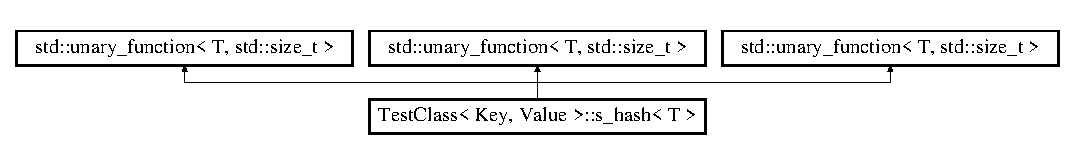
\includegraphics[height=1.562064cm]{struct_test_class_1_1s__hash}
\end{center}
\end{figure}
\subsection*{Public Member Functions}
\begin{DoxyCompactItemize}
\item 
std\+::size\+\_\+t \hyperlink{struct_test_class_1_1s__hash_a2c704f15f20f8c60e417dc709f89a5a1}{operator()} (T const \&k) const 
\item 
std\+::size\+\_\+t \hyperlink{struct_test_class_1_1s__hash_a2c704f15f20f8c60e417dc709f89a5a1}{operator()} (T const \&k) const 
\item 
std\+::size\+\_\+t \hyperlink{struct_test_class_1_1s__hash_a2c704f15f20f8c60e417dc709f89a5a1}{operator()} (T const \&k) const 
\end{DoxyCompactItemize}


\subsection{Member Function Documentation}
\hypertarget{struct_test_class_1_1s__hash_a2c704f15f20f8c60e417dc709f89a5a1}{}\index{Test\+Class\+::s\+\_\+hash@{Test\+Class\+::s\+\_\+hash}!operator()@{operator()}}
\index{operator()@{operator()}!Test\+Class\+::s\+\_\+hash@{Test\+Class\+::s\+\_\+hash}}
\subsubsection[{operator()(\+T const \&k) const }]{\setlength{\rightskip}{0pt plus 5cm}template$<$class Key, class Value$>$ template$<$class T $>$ std\+::size\+\_\+t {\bf Test\+Class}$<$ Key, {\bf Value} $>$\+::{\bf s\+\_\+hash}$<$ T $>$\+::operator() (
\begin{DoxyParamCaption}
\item[{T const \&}]{k}
\end{DoxyParamCaption}
) const\hspace{0.3cm}{\ttfamily [inline]}}\label{struct_test_class_1_1s__hash_a2c704f15f20f8c60e417dc709f89a5a1}
\hypertarget{struct_test_class_1_1s__hash_a2c704f15f20f8c60e417dc709f89a5a1}{}\index{Test\+Class\+::s\+\_\+hash@{Test\+Class\+::s\+\_\+hash}!operator()@{operator()}}
\index{operator()@{operator()}!Test\+Class\+::s\+\_\+hash@{Test\+Class\+::s\+\_\+hash}}
\subsubsection[{operator()(\+T const \&k) const }]{\setlength{\rightskip}{0pt plus 5cm}template$<$class Key, class Value$>$ template$<$class T $>$ std\+::size\+\_\+t {\bf Test\+Class}$<$ Key, {\bf Value} $>$\+::{\bf s\+\_\+hash}$<$ T $>$\+::operator() (
\begin{DoxyParamCaption}
\item[{T const \&}]{k}
\end{DoxyParamCaption}
) const\hspace{0.3cm}{\ttfamily [inline]}}\label{struct_test_class_1_1s__hash_a2c704f15f20f8c60e417dc709f89a5a1}
\hypertarget{struct_test_class_1_1s__hash_a2c704f15f20f8c60e417dc709f89a5a1}{}\index{Test\+Class\+::s\+\_\+hash@{Test\+Class\+::s\+\_\+hash}!operator()@{operator()}}
\index{operator()@{operator()}!Test\+Class\+::s\+\_\+hash@{Test\+Class\+::s\+\_\+hash}}
\subsubsection[{operator()(\+T const \&k) const }]{\setlength{\rightskip}{0pt plus 5cm}template$<$class Key, class Value$>$ template$<$class T $>$ std\+::size\+\_\+t {\bf Test\+Class}$<$ Key, {\bf Value} $>$\+::{\bf s\+\_\+hash}$<$ T $>$\+::operator() (
\begin{DoxyParamCaption}
\item[{T const \&}]{k}
\end{DoxyParamCaption}
) const\hspace{0.3cm}{\ttfamily [inline]}}\label{struct_test_class_1_1s__hash_a2c704f15f20f8c60e417dc709f89a5a1}


The documentation for this struct was generated from the following files\+:\begin{DoxyCompactItemize}
\item 
tervel/tests/hash\+\_\+map/api/\hyperlink{cds__split__map_8h}{cds\+\_\+split\+\_\+map.\+h}\item 
tervel/tests/hash\+\_\+map/api/\hyperlink{lock__boost__map_8h}{lock\+\_\+boost\+\_\+map.\+h}\item 
tervel/tests/hash\+\_\+map/api/\hyperlink{lock__stl__map_8h}{lock\+\_\+stl\+\_\+map.\+h}\end{DoxyCompactItemize}

\hypertarget{class_shift_helper}{}\section{Shift\+Helper$<$ Shift\+Op, T $>$ Class Template Reference}
\label{class_shift_helper}\index{Shift\+Helper$<$ Shift\+Op, T $>$@{Shift\+Helper$<$ Shift\+Op, T $>$}}


{\ttfamily \#include $<$shift\+\_\+helper.\+h$>$}

Inheritance diagram for Shift\+Helper$<$ Shift\+Op, T $>$\+:\begin{figure}[H]
\begin{center}
\leavevmode
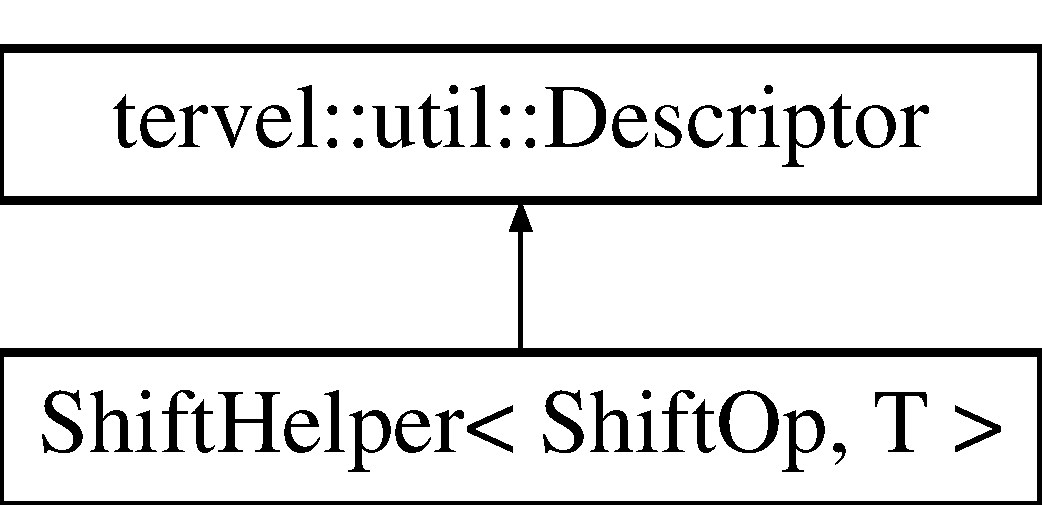
\includegraphics[height=2.000000cm]{class_shift_helper}
\end{center}
\end{figure}
\subsection*{Public Member Functions}
\begin{DoxyCompactItemize}
\item 
\hyperlink{class_shift_helper_afe59d3f3c04ec220e27b4e105ef524ba}{Shift\+Helper} (Shift\+Op $\ast$op\+\_\+rec, \hyperlink{class_shift_helper_a4aef867507bfd1c5db6c66d3902c1ac4}{helper\+\_\+t} $\ast$prev, T replaced\+\_\+value)
\item 
bool \hyperlink{class_shift_helper_aff4a4245b9e9abd04924b5786a11f865}{complete\+\_\+phase1} (W\+F\+Vector $\ast$vec, int pos)
\item 
bool \hyperlink{class_shift_helper_a767a40e252dfebb4b281a6c10a079056}{complete} (W\+F\+Vector $\ast$vec, int pos)
\item 
bool \hyperlink{class_shift_helper_ad7f8e39f62c9646ec5862df3ee1e5ab4}{on\+\_\+watch} (std\+::atomic$<$ void $\ast$ $>$ $\ast$address, void $\ast$value)
\begin{DoxyCompactList}\small\item\em This method is optional to implement for each sub class. \end{DoxyCompactList}\item 
void $\ast$ \hyperlink{class_shift_helper_a4c58f2e7ae4ce7e86a38fea777b3ff2e}{get\+\_\+logical\+\_\+value} ()
\begin{DoxyCompactList}\small\item\em This method is implemented by each sub class. \end{DoxyCompactList}\item 
{\footnotesize template$<$$>$ }\\bool \hyperlink{class_shift_helper_a16fb2a9b85184a6df079d24be1fa407d}{complete} (W\+F\+Vector $\ast$vec, int pos)
\item 
{\footnotesize template$<$$>$ }\\bool \hyperlink{class_shift_helper_a08b8565cd212f551818204c94430d579}{complete} (W\+F\+Vector $\ast$vec, int pos)
\end{DoxyCompactItemize}
\subsection*{Public Attributes}
\begin{DoxyCompactItemize}
\item 
const \hyperlink{class_shift_helper_a4aef867507bfd1c5db6c66d3902c1ac4}{helper\+\_\+t} $\ast$ \hyperlink{class_shift_helper_a78998ae32b1b34120e66ab954a5faeca}{prev\+\_\+}
\item 
const Shift\+Op $\ast$ \hyperlink{class_shift_helper_aed2e1221ed06fb90eb37979339229ef9}{op\+\_\+rec\+\_\+}
\item 
const T \hyperlink{class_shift_helper_ad138be20f4364f297e3c809eda6136c4}{replaced\+\_\+value\+\_\+}
\item 
std\+::atomic$<$ \hyperlink{class_shift_helper_a4aef867507bfd1c5db6c66d3902c1ac4}{helper\+\_\+t} $\ast$ $>$ \hyperlink{class_shift_helper_a04a511ddc0133148d98c38cad0a73e16}{next\+\_\+} \{nullptr\}
\end{DoxyCompactItemize}
\subsection*{Private Types}
\begin{DoxyCompactItemize}
\item 
typedef \hyperlink{class_shift_helper}{Shift\+Helper}$<$ Shift\+Op, T $>$ \hyperlink{class_shift_helper_a4aef867507bfd1c5db6c66d3902c1ac4}{helper\+\_\+t}
\end{DoxyCompactItemize}


\subsection{Member Typedef Documentation}
\hypertarget{class_shift_helper_a4aef867507bfd1c5db6c66d3902c1ac4}{}\index{Shift\+Helper@{Shift\+Helper}!helper\+\_\+t@{helper\+\_\+t}}
\index{helper\+\_\+t@{helper\+\_\+t}!Shift\+Helper@{Shift\+Helper}}
\subsubsection[{helper\+\_\+t}]{\setlength{\rightskip}{0pt plus 5cm}template$<$class Shift\+Op, class T$>$ typedef {\bf Shift\+Helper}$<$Shift\+Op, T$>$ {\bf Shift\+Helper}$<$ Shift\+Op, T $>$\+::{\bf helper\+\_\+t}\hspace{0.3cm}{\ttfamily [private]}}\label{class_shift_helper_a4aef867507bfd1c5db6c66d3902c1ac4}


\subsection{Constructor \& Destructor Documentation}
\hypertarget{class_shift_helper_afe59d3f3c04ec220e27b4e105ef524ba}{}\index{Shift\+Helper@{Shift\+Helper}!Shift\+Helper@{Shift\+Helper}}
\index{Shift\+Helper@{Shift\+Helper}!Shift\+Helper@{Shift\+Helper}}
\subsubsection[{Shift\+Helper(\+Shift\+Op $\ast$op\+\_\+rec, helper\+\_\+t $\ast$prev, T replaced\+\_\+value)}]{\setlength{\rightskip}{0pt plus 5cm}template$<$class Shift\+Op, class T$>$ {\bf Shift\+Helper}$<$ Shift\+Op, T $>$\+::{\bf Shift\+Helper} (
\begin{DoxyParamCaption}
\item[{Shift\+Op $\ast$}]{op\+\_\+rec, }
\item[{{\bf helper\+\_\+t} $\ast$}]{prev, }
\item[{T}]{replaced\+\_\+value}
\end{DoxyParamCaption}
)\hspace{0.3cm}{\ttfamily [inline]}}\label{class_shift_helper_afe59d3f3c04ec220e27b4e105ef524ba}


\subsection{Member Function Documentation}
\hypertarget{class_shift_helper_a767a40e252dfebb4b281a6c10a079056}{}\index{Shift\+Helper@{Shift\+Helper}!complete@{complete}}
\index{complete@{complete}!Shift\+Helper@{Shift\+Helper}}
\subsubsection[{complete(\+W\+F\+Vector $\ast$vec, int pos)}]{\setlength{\rightskip}{0pt plus 5cm}template$<$class Shift\+Op, class T$>$ bool {\bf Shift\+Helper}$<$ Shift\+Op, T $>$\+::complete (
\begin{DoxyParamCaption}
\item[{W\+F\+Vector $\ast$}]{vec, }
\item[{int}]{pos}
\end{DoxyParamCaption}
)}\label{class_shift_helper_a767a40e252dfebb4b281a6c10a079056}
\hypertarget{class_shift_helper_a16fb2a9b85184a6df079d24be1fa407d}{}\index{Shift\+Helper@{Shift\+Helper}!complete@{complete}}
\index{complete@{complete}!Shift\+Helper@{Shift\+Helper}}
\subsubsection[{complete(\+W\+F\+Vector $\ast$vec, int pos)}]{\setlength{\rightskip}{0pt plus 5cm}template$<$$>$ bool {\bf Shift\+Helper}$<$ {\bf Insert\+At} $>$\+::complete (
\begin{DoxyParamCaption}
\item[{W\+F\+Vector $\ast$}]{vec, }
\item[{int}]{pos}
\end{DoxyParamCaption}
)}\label{class_shift_helper_a16fb2a9b85184a6df079d24be1fa407d}
\hypertarget{class_shift_helper_a08b8565cd212f551818204c94430d579}{}\index{Shift\+Helper@{Shift\+Helper}!complete@{complete}}
\index{complete@{complete}!Shift\+Helper@{Shift\+Helper}}
\subsubsection[{complete(\+W\+F\+Vector $\ast$vec, int pos)}]{\setlength{\rightskip}{0pt plus 5cm}template$<$$>$ bool {\bf Shift\+Helper}$<$ {\bf Erase\+At} $>$\+::complete (
\begin{DoxyParamCaption}
\item[{W\+F\+Vector $\ast$}]{vec, }
\item[{int}]{pos}
\end{DoxyParamCaption}
)}\label{class_shift_helper_a08b8565cd212f551818204c94430d579}
\hypertarget{class_shift_helper_aff4a4245b9e9abd04924b5786a11f865}{}\index{Shift\+Helper@{Shift\+Helper}!complete\+\_\+phase1@{complete\+\_\+phase1}}
\index{complete\+\_\+phase1@{complete\+\_\+phase1}!Shift\+Helper@{Shift\+Helper}}
\subsubsection[{complete\+\_\+phase1(\+W\+F\+Vector $\ast$vec, int pos)}]{\setlength{\rightskip}{0pt plus 5cm}template$<$class Parent\+Op $>$ bool {\bf Shift\+Helper}$<$ Parent\+Op $>$\+::complete\+\_\+phase1 (
\begin{DoxyParamCaption}
\item[{W\+F\+Vector $\ast$}]{vec, }
\item[{int}]{pos}
\end{DoxyParamCaption}
)}\label{class_shift_helper_aff4a4245b9e9abd04924b5786a11f865}
\hypertarget{class_shift_helper_a4c58f2e7ae4ce7e86a38fea777b3ff2e}{}\index{Shift\+Helper@{Shift\+Helper}!get\+\_\+logical\+\_\+value@{get\+\_\+logical\+\_\+value}}
\index{get\+\_\+logical\+\_\+value@{get\+\_\+logical\+\_\+value}!Shift\+Helper@{Shift\+Helper}}
\subsubsection[{get\+\_\+logical\+\_\+value()}]{\setlength{\rightskip}{0pt plus 5cm}template$<$class Shift\+Op, class T$>$ void$\ast$ {\bf Shift\+Helper}$<$ Shift\+Op, T $>$\+::get\+\_\+logical\+\_\+value (
\begin{DoxyParamCaption}
{}
\end{DoxyParamCaption}
)\hspace{0.3cm}{\ttfamily [inline]}, {\ttfamily [virtual]}}\label{class_shift_helper_a4c58f2e7ae4ce7e86a38fea777b3ff2e}


This method is implemented by each sub class. 

It returns the logical value of the past address. If the associated operation is still in progress then it will generally return the value that was replaced by this descriptor. Otherwise it will generally return the result of the operation for the specified address.

It can only be called from the static function which protects the object from being reused during the function. 

Implements \hyperlink{classtervel_1_1util_1_1_descriptor_a5b443eeb6acf1207f27a6d06c39d4ad4}{tervel\+::util\+::\+Descriptor}.

\hypertarget{class_shift_helper_ad7f8e39f62c9646ec5862df3ee1e5ab4}{}\index{Shift\+Helper@{Shift\+Helper}!on\+\_\+watch@{on\+\_\+watch}}
\index{on\+\_\+watch@{on\+\_\+watch}!Shift\+Helper@{Shift\+Helper}}
\subsubsection[{on\+\_\+watch(std\+::atomic$<$ void $\ast$ $>$ $\ast$address, void $\ast$value)}]{\setlength{\rightskip}{0pt plus 5cm}template$<$class Shift\+Op, class T$>$ bool {\bf Shift\+Helper}$<$ Shift\+Op, T $>$\+::on\+\_\+watch (
\begin{DoxyParamCaption}
\item[{std\+::atomic$<$ void $\ast$ $>$ $\ast$}]{, }
\item[{void $\ast$}]{}
\end{DoxyParamCaption}
)\hspace{0.3cm}{\ttfamily [inline]}, {\ttfamily [virtual]}}\label{class_shift_helper_ad7f8e39f62c9646ec5862df3ee1e5ab4}


This method is optional to implement for each sub class. 

In the event there is a complex dependency between descriptor objects, where watching one implies performing other actions, such as watching a parent object, a developer will implement this function to encapsulate that logic

This function is called by the static watch function It should not watch itself.


\begin{DoxyParams}{Parameters}
{\em address} & The location to check. \\
\hline
{\em expected} & The expected value for that location\\
\hline
\end{DoxyParams}
\begin{DoxyReturn}{Returns}
true if successful, false otherwise 
\end{DoxyReturn}


Reimplemented from \hyperlink{classtervel_1_1util_1_1_descriptor_ab643e09f20f35149dc820766b0f9ccdb}{tervel\+::util\+::\+Descriptor}.



\subsection{Member Data Documentation}
\hypertarget{class_shift_helper_a04a511ddc0133148d98c38cad0a73e16}{}\index{Shift\+Helper@{Shift\+Helper}!next\+\_\+@{next\+\_\+}}
\index{next\+\_\+@{next\+\_\+}!Shift\+Helper@{Shift\+Helper}}
\subsubsection[{next\+\_\+}]{\setlength{\rightskip}{0pt plus 5cm}template$<$class Shift\+Op, class T$>$ std\+::atomic$<${\bf helper\+\_\+t} $\ast$$>$ {\bf Shift\+Helper}$<$ Shift\+Op, T $>$\+::next\+\_\+ \{nullptr\}}\label{class_shift_helper_a04a511ddc0133148d98c38cad0a73e16}
\hypertarget{class_shift_helper_aed2e1221ed06fb90eb37979339229ef9}{}\index{Shift\+Helper@{Shift\+Helper}!op\+\_\+rec\+\_\+@{op\+\_\+rec\+\_\+}}
\index{op\+\_\+rec\+\_\+@{op\+\_\+rec\+\_\+}!Shift\+Helper@{Shift\+Helper}}
\subsubsection[{op\+\_\+rec\+\_\+}]{\setlength{\rightskip}{0pt plus 5cm}template$<$class Shift\+Op, class T$>$ const Shift\+Op$\ast$ {\bf Shift\+Helper}$<$ Shift\+Op, T $>$\+::op\+\_\+rec\+\_\+}\label{class_shift_helper_aed2e1221ed06fb90eb37979339229ef9}
\hypertarget{class_shift_helper_a78998ae32b1b34120e66ab954a5faeca}{}\index{Shift\+Helper@{Shift\+Helper}!prev\+\_\+@{prev\+\_\+}}
\index{prev\+\_\+@{prev\+\_\+}!Shift\+Helper@{Shift\+Helper}}
\subsubsection[{prev\+\_\+}]{\setlength{\rightskip}{0pt plus 5cm}template$<$class Shift\+Op, class T$>$ const {\bf helper\+\_\+t}$\ast$ {\bf Shift\+Helper}$<$ Shift\+Op, T $>$\+::prev\+\_\+}\label{class_shift_helper_a78998ae32b1b34120e66ab954a5faeca}
\hypertarget{class_shift_helper_ad138be20f4364f297e3c809eda6136c4}{}\index{Shift\+Helper@{Shift\+Helper}!replaced\+\_\+value\+\_\+@{replaced\+\_\+value\+\_\+}}
\index{replaced\+\_\+value\+\_\+@{replaced\+\_\+value\+\_\+}!Shift\+Helper@{Shift\+Helper}}
\subsubsection[{replaced\+\_\+value\+\_\+}]{\setlength{\rightskip}{0pt plus 5cm}template$<$class Shift\+Op, class T$>$ const T {\bf Shift\+Helper}$<$ Shift\+Op, T $>$\+::replaced\+\_\+value\+\_\+}\label{class_shift_helper_ad138be20f4364f297e3c809eda6136c4}


The documentation for this class was generated from the following file\+:\begin{DoxyCompactItemize}
\item 
tervel/containers/wf/vector/old/\hyperlink{shift__helper_8h}{shift\+\_\+helper.\+h}\end{DoxyCompactItemize}

\hypertarget{classtervel_1_1_tervel}{}\section{tervel\+:\+:Tervel Class Reference}
\label{classtervel_1_1_tervel}\index{tervel\+::\+Tervel@{tervel\+::\+Tervel}}


Contains shared information that should be accessible by all threads.  




{\ttfamily \#include $<$tervel.\+h$>$}

\subsection*{Public Member Functions}
\begin{DoxyCompactItemize}
\item 
\hyperlink{classtervel_1_1_tervel_aae87ace03f0fb62083e3683f99135a00}{Tervel} (size\+\_\+t num\+\_\+threads)
\item 
\hyperlink{classtervel_1_1_tervel_aea18e9dcc8a8212c0c451a94bc9ff522}{$\sim$\+Tervel} ()
\end{DoxyCompactItemize}
\subsection*{Private Member Functions}
\begin{DoxyCompactItemize}
\item 
uint64\+\_\+t \hyperlink{classtervel_1_1_tervel_a89db2253e58923a4d113bb3a5f197b47}{get\+\_\+thread\+\_\+id} ()
\item 
\hyperlink{classtervel_1_1_tervel_ae4aafbeaaa2d0c95ca825b3ec9db0c5d}{D\+I\+S\+A\+L\+L\+O\+W\+\_\+\+C\+O\+P\+Y\+\_\+\+A\+N\+D\+\_\+\+A\+S\+S\+I\+G\+N} (\hyperlink{classtervel_1_1_tervel}{Tervel})
\end{DoxyCompactItemize}
\subsection*{Private Attributes}
\begin{DoxyCompactItemize}
\item 
const uint64\+\_\+t \hyperlink{classtervel_1_1_tervel_adc91b4b1b22ab49ed249df0ef14eadad}{num\+\_\+threads\+\_\+}
\item 
std\+::atomic$<$ uint64\+\_\+t $>$ \hyperlink{classtervel_1_1_tervel_a3942b8c533d065ab7df11e20d253afa9}{active\+\_\+threads\+\_\+} \{0\}
\item 
\hyperlink{classtervel_1_1util_1_1memory_1_1hp_1_1_hazard_pointer}{util\+::memory\+::hp\+::\+Hazard\+Pointer} \hyperlink{classtervel_1_1_tervel_aa0d6c90c07f50e9505b2ac590425a59a}{hazard\+\_\+pointer\+\_\+}
\item 
\hyperlink{classtervel_1_1util_1_1memory_1_1rc_1_1_pool_manager}{util\+::memory\+::rc\+::\+Pool\+Manager} \hyperlink{classtervel_1_1_tervel_a86681b7ea969722f86234c70b9d97a83}{rc\+\_\+pool\+\_\+manager\+\_\+}
\item 
\hyperlink{classtervel_1_1util_1_1_progress_assurance}{util\+::\+Progress\+Assurance} \hyperlink{classtervel_1_1_tervel_a011a5b3732c1482ac6cc87cb47d20b42}{progress\+\_\+assurance\+\_\+}
\item 
friend \hyperlink{classtervel_1_1_tervel_a6322cb41e5b57f070b02dd1b1f54cea2}{Thread\+Context}
\end{DoxyCompactItemize}


\subsection{Detailed Description}
Contains shared information that should be accessible by all threads. 

\subsection{Constructor \& Destructor Documentation}
\hypertarget{classtervel_1_1_tervel_aae87ace03f0fb62083e3683f99135a00}{}\index{tervel\+::\+Tervel@{tervel\+::\+Tervel}!Tervel@{Tervel}}
\index{Tervel@{Tervel}!tervel\+::\+Tervel@{tervel\+::\+Tervel}}
\subsubsection[{Tervel(size\+\_\+t num\+\_\+threads)}]{\setlength{\rightskip}{0pt plus 5cm}tervel\+::\+Tervel\+::\+Tervel (
\begin{DoxyParamCaption}
\item[{size\+\_\+t}]{num\+\_\+threads}
\end{DoxyParamCaption}
)\hspace{0.3cm}{\ttfamily [inline]}, {\ttfamily [explicit]}}\label{classtervel_1_1_tervel_aae87ace03f0fb62083e3683f99135a00}
\hypertarget{classtervel_1_1_tervel_aea18e9dcc8a8212c0c451a94bc9ff522}{}\index{tervel\+::\+Tervel@{tervel\+::\+Tervel}!````~Tervel@{$\sim$\+Tervel}}
\index{````~Tervel@{$\sim$\+Tervel}!tervel\+::\+Tervel@{tervel\+::\+Tervel}}
\subsubsection[{$\sim$\+Tervel()}]{\setlength{\rightskip}{0pt plus 5cm}tervel\+::\+Tervel\+::$\sim$\+Tervel (
\begin{DoxyParamCaption}
{}
\end{DoxyParamCaption}
)\hspace{0.3cm}{\ttfamily [inline]}}\label{classtervel_1_1_tervel_aea18e9dcc8a8212c0c451a94bc9ff522}


\subsection{Member Function Documentation}
\hypertarget{classtervel_1_1_tervel_ae4aafbeaaa2d0c95ca825b3ec9db0c5d}{}\index{tervel\+::\+Tervel@{tervel\+::\+Tervel}!D\+I\+S\+A\+L\+L\+O\+W\+\_\+\+C\+O\+P\+Y\+\_\+\+A\+N\+D\+\_\+\+A\+S\+S\+I\+G\+N@{D\+I\+S\+A\+L\+L\+O\+W\+\_\+\+C\+O\+P\+Y\+\_\+\+A\+N\+D\+\_\+\+A\+S\+S\+I\+G\+N}}
\index{D\+I\+S\+A\+L\+L\+O\+W\+\_\+\+C\+O\+P\+Y\+\_\+\+A\+N\+D\+\_\+\+A\+S\+S\+I\+G\+N@{D\+I\+S\+A\+L\+L\+O\+W\+\_\+\+C\+O\+P\+Y\+\_\+\+A\+N\+D\+\_\+\+A\+S\+S\+I\+G\+N}!tervel\+::\+Tervel@{tervel\+::\+Tervel}}
\subsubsection[{D\+I\+S\+A\+L\+L\+O\+W\+\_\+\+C\+O\+P\+Y\+\_\+\+A\+N\+D\+\_\+\+A\+S\+S\+I\+G\+N(\+Tervel)}]{\setlength{\rightskip}{0pt plus 5cm}tervel\+::\+Tervel\+::\+D\+I\+S\+A\+L\+L\+O\+W\+\_\+\+C\+O\+P\+Y\+\_\+\+A\+N\+D\+\_\+\+A\+S\+S\+I\+G\+N (
\begin{DoxyParamCaption}
\item[{{\bf Tervel}}]{}
\end{DoxyParamCaption}
)\hspace{0.3cm}{\ttfamily [private]}}\label{classtervel_1_1_tervel_ae4aafbeaaa2d0c95ca825b3ec9db0c5d}
\hypertarget{classtervel_1_1_tervel_a89db2253e58923a4d113bb3a5f197b47}{}\index{tervel\+::\+Tervel@{tervel\+::\+Tervel}!get\+\_\+thread\+\_\+id@{get\+\_\+thread\+\_\+id}}
\index{get\+\_\+thread\+\_\+id@{get\+\_\+thread\+\_\+id}!tervel\+::\+Tervel@{tervel\+::\+Tervel}}
\subsubsection[{get\+\_\+thread\+\_\+id()}]{\setlength{\rightskip}{0pt plus 5cm}uint64\+\_\+t tervel\+::\+Tervel\+::get\+\_\+thread\+\_\+id (
\begin{DoxyParamCaption}
{}
\end{DoxyParamCaption}
)\hspace{0.3cm}{\ttfamily [inline]}, {\ttfamily [private]}}\label{classtervel_1_1_tervel_a89db2253e58923a4d113bb3a5f197b47}


\subsection{Member Data Documentation}
\hypertarget{classtervel_1_1_tervel_a3942b8c533d065ab7df11e20d253afa9}{}\index{tervel\+::\+Tervel@{tervel\+::\+Tervel}!active\+\_\+threads\+\_\+@{active\+\_\+threads\+\_\+}}
\index{active\+\_\+threads\+\_\+@{active\+\_\+threads\+\_\+}!tervel\+::\+Tervel@{tervel\+::\+Tervel}}
\subsubsection[{active\+\_\+threads\+\_\+}]{\setlength{\rightskip}{0pt plus 5cm}std\+::atomic$<$uint64\+\_\+t$>$ tervel\+::\+Tervel\+::active\+\_\+threads\+\_\+ \{0\}\hspace{0.3cm}{\ttfamily [private]}}\label{classtervel_1_1_tervel_a3942b8c533d065ab7df11e20d253afa9}
\hypertarget{classtervel_1_1_tervel_aa0d6c90c07f50e9505b2ac590425a59a}{}\index{tervel\+::\+Tervel@{tervel\+::\+Tervel}!hazard\+\_\+pointer\+\_\+@{hazard\+\_\+pointer\+\_\+}}
\index{hazard\+\_\+pointer\+\_\+@{hazard\+\_\+pointer\+\_\+}!tervel\+::\+Tervel@{tervel\+::\+Tervel}}
\subsubsection[{hazard\+\_\+pointer\+\_\+}]{\setlength{\rightskip}{0pt plus 5cm}{\bf util\+::memory\+::hp\+::\+Hazard\+Pointer} tervel\+::\+Tervel\+::hazard\+\_\+pointer\+\_\+\hspace{0.3cm}{\ttfamily [private]}}\label{classtervel_1_1_tervel_aa0d6c90c07f50e9505b2ac590425a59a}
\hypertarget{classtervel_1_1_tervel_adc91b4b1b22ab49ed249df0ef14eadad}{}\index{tervel\+::\+Tervel@{tervel\+::\+Tervel}!num\+\_\+threads\+\_\+@{num\+\_\+threads\+\_\+}}
\index{num\+\_\+threads\+\_\+@{num\+\_\+threads\+\_\+}!tervel\+::\+Tervel@{tervel\+::\+Tervel}}
\subsubsection[{num\+\_\+threads\+\_\+}]{\setlength{\rightskip}{0pt plus 5cm}const uint64\+\_\+t tervel\+::\+Tervel\+::num\+\_\+threads\+\_\+\hspace{0.3cm}{\ttfamily [private]}}\label{classtervel_1_1_tervel_adc91b4b1b22ab49ed249df0ef14eadad}
\hypertarget{classtervel_1_1_tervel_a011a5b3732c1482ac6cc87cb47d20b42}{}\index{tervel\+::\+Tervel@{tervel\+::\+Tervel}!progress\+\_\+assurance\+\_\+@{progress\+\_\+assurance\+\_\+}}
\index{progress\+\_\+assurance\+\_\+@{progress\+\_\+assurance\+\_\+}!tervel\+::\+Tervel@{tervel\+::\+Tervel}}
\subsubsection[{progress\+\_\+assurance\+\_\+}]{\setlength{\rightskip}{0pt plus 5cm}{\bf util\+::\+Progress\+Assurance} tervel\+::\+Tervel\+::progress\+\_\+assurance\+\_\+\hspace{0.3cm}{\ttfamily [private]}}\label{classtervel_1_1_tervel_a011a5b3732c1482ac6cc87cb47d20b42}
\hypertarget{classtervel_1_1_tervel_a86681b7ea969722f86234c70b9d97a83}{}\index{tervel\+::\+Tervel@{tervel\+::\+Tervel}!rc\+\_\+pool\+\_\+manager\+\_\+@{rc\+\_\+pool\+\_\+manager\+\_\+}}
\index{rc\+\_\+pool\+\_\+manager\+\_\+@{rc\+\_\+pool\+\_\+manager\+\_\+}!tervel\+::\+Tervel@{tervel\+::\+Tervel}}
\subsubsection[{rc\+\_\+pool\+\_\+manager\+\_\+}]{\setlength{\rightskip}{0pt plus 5cm}{\bf util\+::memory\+::rc\+::\+Pool\+Manager} tervel\+::\+Tervel\+::rc\+\_\+pool\+\_\+manager\+\_\+\hspace{0.3cm}{\ttfamily [private]}}\label{classtervel_1_1_tervel_a86681b7ea969722f86234c70b9d97a83}
\hypertarget{classtervel_1_1_tervel_a6322cb41e5b57f070b02dd1b1f54cea2}{}\index{tervel\+::\+Tervel@{tervel\+::\+Tervel}!Thread\+Context@{Thread\+Context}}
\index{Thread\+Context@{Thread\+Context}!tervel\+::\+Tervel@{tervel\+::\+Tervel}}
\subsubsection[{Thread\+Context}]{\setlength{\rightskip}{0pt plus 5cm}friend tervel\+::\+Tervel\+::\+Thread\+Context\hspace{0.3cm}{\ttfamily [private]}}\label{classtervel_1_1_tervel_a6322cb41e5b57f070b02dd1b1f54cea2}


The documentation for this class was generated from the following file\+:\begin{DoxyCompactItemize}
\item 
tervel/util/\hyperlink{tervel_8h}{tervel.\+h}\end{DoxyCompactItemize}

\hypertarget{class_test_class}{}\section{Test\+Class$<$ Key, Value $>$ Class Template Reference}
\label{class_test_class}\index{Test\+Class$<$ Key, Value $>$@{Test\+Class$<$ Key, Value $>$}}


{\ttfamily \#include $<$blank\+\_\+api.\+h$>$}

\subsection*{Classes}
\begin{DoxyCompactItemize}
\item 
struct \hyperlink{struct_test_class_1_1equal__to}{equal\+\_\+to}
\item 
struct \hyperlink{struct_test_class_1_1foo__set__traits}{foo\+\_\+set\+\_\+traits}
\item 
struct \hyperlink{struct_test_class_1_1functor}{functor}
\item 
struct \hyperlink{struct_test_class_1_1less__s}{less\+\_\+s}
\item 
struct \hyperlink{struct_test_class_1_1list__traits}{list\+\_\+traits}
\item 
struct \hyperlink{struct_test_class_1_1map__traits}{map\+\_\+traits}
\item 
struct \hyperlink{struct_test_class_1_1_my_hash_compare}{My\+Hash\+Compare}
\item 
struct \hyperlink{struct_test_class_1_1s__hash}{s\+\_\+hash}
\item 
struct \hyperlink{struct_test_class_1_1ufunctor}{ufunctor}
\item 
class \hyperlink{class_test_class_1_1_wrapper_type}{Wrapper\+Type}
\end{DoxyCompactItemize}
\subsection*{Public Types}
\begin{DoxyCompactItemize}
\item 
typedef \hyperlink{classtervel_1_1containers_1_1wf_1_1_hash_map}{tervel\+::containers\+::wf\+::\+Hash\+Map}$<$ Key, \hyperlink{hash__map_2test_object_8h_ad777bf08d8e2b01df17ba5e3c51ae11f}{Value} $>$ \hyperlink{class_test_class_a1b85c62e95a514dec1b9680e76348329}{Map}
\item 
typedef \hyperlink{classtervel_1_1containers_1_1wf_1_1_hash_map}{tervel\+::containers\+::wf\+::\+Hash\+Map}$<$ Key, \hyperlink{hash__map_2test_object_8h_ad777bf08d8e2b01df17ba5e3c51ae11f}{Value} $>$\+::Value\+Accessor \hyperlink{class_test_class_a0af9e93839a0717ed717ab4818353762}{Accessor}
\item 
typedef \hyperlink{classtervel_1_1containers_1_1wf_1_1_hash_map}{tervel\+::containers\+::wf\+::\+Hash\+Map}$<$ Key, \hyperlink{hash__map_2test_object_8h_ad777bf08d8e2b01df17ba5e3c51ae11f}{Value} $>$ \hyperlink{class_test_class_a1b85c62e95a514dec1b9680e76348329}{Map}
\item 
typedef \hyperlink{classtervel_1_1containers_1_1wf_1_1_hash_map}{tervel\+::containers\+::wf\+::\+Hash\+Map}$<$ Key, \hyperlink{hash__map_2test_object_8h_ad777bf08d8e2b01df17ba5e3c51ae11f}{Value} $>$\+::Value\+Accessor \hyperlink{class_test_class_a0af9e93839a0717ed717ab4818353762}{Accessor}
\item 
typedef \hyperlink{classtervel_1_1containers_1_1wf_1_1_ring_buffer}{tervel\+::containers\+::wf\+::\+Ring\+Buffer}$<$ \hyperlink{class_test_class_1_1_wrapper_type}{Wrapper\+Type} $\ast$ $>$ \hyperlink{class_test_class_abe640a96ccd2edb9a09ad292c8a8b298}{container\+\_\+t}
\end{DoxyCompactItemize}
\subsection*{Public Member Functions}
\begin{DoxyCompactItemize}
\item 
\hyperlink{class_test_class_ab3dbc7a67da46dda1125f7dee533aca2}{Test\+Class} (size\+\_\+t num\+\_\+threads, size\+\_\+t capacity)
\item 
std\+::string \hyperlink{class_test_class_a84e73a91ede625887472a307235d6de5}{to\+String} ()
\item 
void \hyperlink{class_test_class_a7e6bce4c39c047282ea8c1f1485a260b}{attach\+\_\+thread} ()
\item 
void \hyperlink{class_test_class_a79b3a395c8a1fac7a156228a27d829cc}{detach\+\_\+thread} ()
\item 
bool \hyperlink{class_test_class_af497b95115e81f882851b2ab843c298c}{find} (Key key, \hyperlink{hash__map_2test_object_8h_ad777bf08d8e2b01df17ba5e3c51ae11f}{Value} \&value)
\item 
bool \hyperlink{class_test_class_a0d075565ad4cccdb071bf267fe444681}{insert} (Key key, \hyperlink{hash__map_2test_object_8h_ad777bf08d8e2b01df17ba5e3c51ae11f}{Value} value)
\item 
bool \hyperlink{class_test_class_a4c33c8cac20119f9bee9b5091bc8a385}{update} (Key key, \hyperlink{hash__map_2test_object_8h_ad777bf08d8e2b01df17ba5e3c51ae11f}{Value} \&value\+\_\+expected, \hyperlink{hash__map_2test_object_8h_ad777bf08d8e2b01df17ba5e3c51ae11f}{Value} value\+\_\+new)
\item 
bool \hyperlink{class_test_class_a3a22d60709c15d419f69d29b7de92d02}{remove} (Key key)
\item 
size\+\_\+t \hyperlink{class_test_class_af2230f298ab3ef4ebf71aa7afa3fb6ca}{size} ()
\item 
\hyperlink{class_test_class_ab3dbc7a67da46dda1125f7dee533aca2}{Test\+Class} (size\+\_\+t num\+\_\+threads, size\+\_\+t capacity)
\item 
std\+::string \hyperlink{class_test_class_a84e73a91ede625887472a307235d6de5}{to\+String} ()
\item 
void \hyperlink{class_test_class_a7e6bce4c39c047282ea8c1f1485a260b}{attach\+\_\+thread} ()
\item 
void \hyperlink{class_test_class_a79b3a395c8a1fac7a156228a27d829cc}{detach\+\_\+thread} ()
\item 
bool \hyperlink{class_test_class_af497b95115e81f882851b2ab843c298c}{find} (Key key, \hyperlink{hash__map_2test_object_8h_ad777bf08d8e2b01df17ba5e3c51ae11f}{Value} \&value)
\item 
bool \hyperlink{class_test_class_a0d075565ad4cccdb071bf267fe444681}{insert} (Key key, \hyperlink{hash__map_2test_object_8h_ad777bf08d8e2b01df17ba5e3c51ae11f}{Value} value)
\item 
bool \hyperlink{class_test_class_a4c33c8cac20119f9bee9b5091bc8a385}{update} (Key key, \hyperlink{hash__map_2test_object_8h_ad777bf08d8e2b01df17ba5e3c51ae11f}{Value} \&value\+\_\+expected, \hyperlink{hash__map_2test_object_8h_ad777bf08d8e2b01df17ba5e3c51ae11f}{Value} value\+\_\+new)
\item 
bool \hyperlink{class_test_class_a3a22d60709c15d419f69d29b7de92d02}{remove} (Key key)
\item 
size\+\_\+t \hyperlink{class_test_class_af2230f298ab3ef4ebf71aa7afa3fb6ca}{size} ()
\item 
\hyperlink{class_test_class_ab3dbc7a67da46dda1125f7dee533aca2}{Test\+Class} (size\+\_\+t num\+\_\+threads, size\+\_\+t capacity)
\item 
std\+::string \hyperlink{class_test_class_a84e73a91ede625887472a307235d6de5}{to\+String} ()
\item 
void \hyperlink{class_test_class_a7e6bce4c39c047282ea8c1f1485a260b}{attach\+\_\+thread} ()
\item 
void \hyperlink{class_test_class_a79b3a395c8a1fac7a156228a27d829cc}{detach\+\_\+thread} ()
\item 
bool \hyperlink{class_test_class_af497b95115e81f882851b2ab843c298c}{find} (Key key, \hyperlink{hash__map_2test_object_8h_ad777bf08d8e2b01df17ba5e3c51ae11f}{Value} \&value)
\item 
bool \hyperlink{class_test_class_a0d075565ad4cccdb071bf267fe444681}{insert} (Key key, \hyperlink{hash__map_2test_object_8h_ad777bf08d8e2b01df17ba5e3c51ae11f}{Value} value)
\item 
bool \hyperlink{class_test_class_a4c33c8cac20119f9bee9b5091bc8a385}{update} (Key key, \hyperlink{hash__map_2test_object_8h_ad777bf08d8e2b01df17ba5e3c51ae11f}{Value} \&value\+\_\+expected, \hyperlink{hash__map_2test_object_8h_ad777bf08d8e2b01df17ba5e3c51ae11f}{Value} value\+\_\+new)
\item 
bool \hyperlink{class_test_class_a3a22d60709c15d419f69d29b7de92d02}{remove} (Key key)
\item 
size\+\_\+t \hyperlink{class_test_class_af2230f298ab3ef4ebf71aa7afa3fb6ca}{size} ()
\item 
\hyperlink{class_test_class_ab3dbc7a67da46dda1125f7dee533aca2}{Test\+Class} (size\+\_\+t num\+\_\+threads, size\+\_\+t capacity)
\item 
std\+::string \hyperlink{class_test_class_a84e73a91ede625887472a307235d6de5}{to\+String} ()
\item 
void \hyperlink{class_test_class_a7e6bce4c39c047282ea8c1f1485a260b}{attach\+\_\+thread} ()
\item 
void \hyperlink{class_test_class_a79b3a395c8a1fac7a156228a27d829cc}{detach\+\_\+thread} ()
\item 
bool \hyperlink{class_test_class_af497b95115e81f882851b2ab843c298c}{find} (Key key, \hyperlink{hash__map_2test_object_8h_ad777bf08d8e2b01df17ba5e3c51ae11f}{Value} \&value)
\item 
bool \hyperlink{class_test_class_a0d075565ad4cccdb071bf267fe444681}{insert} (Key key, \hyperlink{hash__map_2test_object_8h_ad777bf08d8e2b01df17ba5e3c51ae11f}{Value} value)
\item 
bool \hyperlink{class_test_class_a4c33c8cac20119f9bee9b5091bc8a385}{update} (Key key, \hyperlink{hash__map_2test_object_8h_ad777bf08d8e2b01df17ba5e3c51ae11f}{Value} \&value\+\_\+expected, \hyperlink{hash__map_2test_object_8h_ad777bf08d8e2b01df17ba5e3c51ae11f}{Value} value\+\_\+new)
\item 
bool \hyperlink{class_test_class_a3a22d60709c15d419f69d29b7de92d02}{remove} (Key key)
\item 
size\+\_\+t \hyperlink{class_test_class_af2230f298ab3ef4ebf71aa7afa3fb6ca}{size} ()
\item 
\hyperlink{class_test_class_ab3dbc7a67da46dda1125f7dee533aca2}{Test\+Class} (size\+\_\+t num\+\_\+threads, size\+\_\+t capacity)
\item 
std\+::string \hyperlink{class_test_class_a84e73a91ede625887472a307235d6de5}{to\+String} ()
\item 
void \hyperlink{class_test_class_a7e6bce4c39c047282ea8c1f1485a260b}{attach\+\_\+thread} ()
\item 
void \hyperlink{class_test_class_a79b3a395c8a1fac7a156228a27d829cc}{detach\+\_\+thread} ()
\item 
bool \hyperlink{class_test_class_af497b95115e81f882851b2ab843c298c}{find} (Key key, \hyperlink{hash__map_2test_object_8h_ad777bf08d8e2b01df17ba5e3c51ae11f}{Value} \&value)
\item 
bool \hyperlink{class_test_class_a0d075565ad4cccdb071bf267fe444681}{insert} (Key key, \hyperlink{hash__map_2test_object_8h_ad777bf08d8e2b01df17ba5e3c51ae11f}{Value} value)
\item 
bool \hyperlink{class_test_class_a4c33c8cac20119f9bee9b5091bc8a385}{update} (Key key, \hyperlink{hash__map_2test_object_8h_ad777bf08d8e2b01df17ba5e3c51ae11f}{Value} \&value\+\_\+expected, \hyperlink{hash__map_2test_object_8h_ad777bf08d8e2b01df17ba5e3c51ae11f}{Value} value\+\_\+new)
\item 
bool \hyperlink{class_test_class_a3a22d60709c15d419f69d29b7de92d02}{remove} (Key key)
\item 
size\+\_\+t \hyperlink{class_test_class_af2230f298ab3ef4ebf71aa7afa3fb6ca}{size} ()
\item 
\hyperlink{class_test_class_ab3dbc7a67da46dda1125f7dee533aca2}{Test\+Class} (size\+\_\+t num\+\_\+threads, size\+\_\+t capacity)
\item 
std\+::string \hyperlink{class_test_class_a84e73a91ede625887472a307235d6de5}{to\+String} ()
\item 
void \hyperlink{class_test_class_a7e6bce4c39c047282ea8c1f1485a260b}{attach\+\_\+thread} ()
\item 
void \hyperlink{class_test_class_a79b3a395c8a1fac7a156228a27d829cc}{detach\+\_\+thread} ()
\item 
bool \hyperlink{class_test_class_af497b95115e81f882851b2ab843c298c}{find} (Key key, \hyperlink{hash__map_2test_object_8h_ad777bf08d8e2b01df17ba5e3c51ae11f}{Value} \&value)
\item 
bool \hyperlink{class_test_class_a0d075565ad4cccdb071bf267fe444681}{insert} (Key key, \hyperlink{hash__map_2test_object_8h_ad777bf08d8e2b01df17ba5e3c51ae11f}{Value} value)
\item 
bool \hyperlink{class_test_class_a4c33c8cac20119f9bee9b5091bc8a385}{update} (Key key, \hyperlink{hash__map_2test_object_8h_ad777bf08d8e2b01df17ba5e3c51ae11f}{Value} \&value\+\_\+expected, \hyperlink{hash__map_2test_object_8h_ad777bf08d8e2b01df17ba5e3c51ae11f}{Value} value\+\_\+new)
\item 
bool \hyperlink{class_test_class_a3a22d60709c15d419f69d29b7de92d02}{remove} (Key key)
\item 
size\+\_\+t \hyperlink{class_test_class_af2230f298ab3ef4ebf71aa7afa3fb6ca}{size} ()
\item 
\hyperlink{class_test_class_ab3dbc7a67da46dda1125f7dee533aca2}{Test\+Class} (size\+\_\+t num\+\_\+threads, size\+\_\+t capacity)
\item 
std\+::string \hyperlink{class_test_class_a84e73a91ede625887472a307235d6de5}{to\+String} ()
\item 
void \hyperlink{class_test_class_a7e6bce4c39c047282ea8c1f1485a260b}{attach\+\_\+thread} ()
\item 
void \hyperlink{class_test_class_a79b3a395c8a1fac7a156228a27d829cc}{detach\+\_\+thread} ()
\item 
bool \hyperlink{class_test_class_af497b95115e81f882851b2ab843c298c}{find} (Key key, \hyperlink{hash__map_2test_object_8h_ad777bf08d8e2b01df17ba5e3c51ae11f}{Value} \&value)
\item 
bool \hyperlink{class_test_class_a0d075565ad4cccdb071bf267fe444681}{insert} (Key key, \hyperlink{hash__map_2test_object_8h_ad777bf08d8e2b01df17ba5e3c51ae11f}{Value} value)
\item 
bool \hyperlink{class_test_class_a4c33c8cac20119f9bee9b5091bc8a385}{update} (Key key, \hyperlink{hash__map_2test_object_8h_ad777bf08d8e2b01df17ba5e3c51ae11f}{Value} \&value\+\_\+expected, \hyperlink{hash__map_2test_object_8h_ad777bf08d8e2b01df17ba5e3c51ae11f}{Value} value\+\_\+new)
\item 
bool \hyperlink{class_test_class_a3a22d60709c15d419f69d29b7de92d02}{remove} (Key key)
\item 
size\+\_\+t \hyperlink{class_test_class_af2230f298ab3ef4ebf71aa7afa3fb6ca}{size} ()
\item 
\hyperlink{class_test_class_ab3dbc7a67da46dda1125f7dee533aca2}{Test\+Class} (size\+\_\+t num\+\_\+threads, size\+\_\+t capacity)
\item 
std\+::string \hyperlink{class_test_class_a84e73a91ede625887472a307235d6de5}{to\+String} ()
\item 
void \hyperlink{class_test_class_a7e6bce4c39c047282ea8c1f1485a260b}{attach\+\_\+thread} ()
\item 
void \hyperlink{class_test_class_a79b3a395c8a1fac7a156228a27d829cc}{detach\+\_\+thread} ()
\item 
bool \hyperlink{class_test_class_af497b95115e81f882851b2ab843c298c}{find} (Key key, \hyperlink{hash__map_2test_object_8h_ad777bf08d8e2b01df17ba5e3c51ae11f}{Value} \&value)
\item 
bool \hyperlink{class_test_class_a0d075565ad4cccdb071bf267fe444681}{insert} (Key key, \hyperlink{hash__map_2test_object_8h_ad777bf08d8e2b01df17ba5e3c51ae11f}{Value} value)
\item 
bool \hyperlink{class_test_class_a4c33c8cac20119f9bee9b5091bc8a385}{update} (Key key, \hyperlink{hash__map_2test_object_8h_ad777bf08d8e2b01df17ba5e3c51ae11f}{Value} \&value\+\_\+expected, \hyperlink{hash__map_2test_object_8h_ad777bf08d8e2b01df17ba5e3c51ae11f}{Value} value\+\_\+new)
\item 
bool \hyperlink{class_test_class_a3a22d60709c15d419f69d29b7de92d02}{remove} (Key key)
\item 
size\+\_\+t \hyperlink{class_test_class_af2230f298ab3ef4ebf71aa7afa3fb6ca}{size} ()
\item 
\hyperlink{class_test_class_ab3dbc7a67da46dda1125f7dee533aca2}{Test\+Class} (size\+\_\+t num\+\_\+threads, size\+\_\+t capacity)
\item 
std\+::string \hyperlink{class_test_class_a84e73a91ede625887472a307235d6de5}{to\+String} ()
\item 
void \hyperlink{class_test_class_a7e6bce4c39c047282ea8c1f1485a260b}{attach\+\_\+thread} ()
\item 
void \hyperlink{class_test_class_a79b3a395c8a1fac7a156228a27d829cc}{detach\+\_\+thread} ()
\item 
bool \hyperlink{class_test_class_af497b95115e81f882851b2ab843c298c}{find} (Key key, \hyperlink{hash__map_2test_object_8h_ad777bf08d8e2b01df17ba5e3c51ae11f}{Value} \&value)
\item 
bool \hyperlink{class_test_class_a0d075565ad4cccdb071bf267fe444681}{insert} (Key key, \hyperlink{hash__map_2test_object_8h_ad777bf08d8e2b01df17ba5e3c51ae11f}{Value} value)
\item 
bool \hyperlink{class_test_class_a4c33c8cac20119f9bee9b5091bc8a385}{update} (Key key, \hyperlink{hash__map_2test_object_8h_ad777bf08d8e2b01df17ba5e3c51ae11f}{Value} \&value\+\_\+expected, \hyperlink{hash__map_2test_object_8h_ad777bf08d8e2b01df17ba5e3c51ae11f}{Value} value\+\_\+new)
\item 
bool \hyperlink{class_test_class_a3a22d60709c15d419f69d29b7de92d02}{remove} (Key key)
\item 
size\+\_\+t \hyperlink{class_test_class_af2230f298ab3ef4ebf71aa7afa3fb6ca}{size} ()
\item 
\hyperlink{class_test_class_a25153d9821ce372f9c9146891b04aa07}{Test\+Class} (size\+\_\+t num\+\_\+threads)
\item 
std\+::string \hyperlink{class_test_class_a84e73a91ede625887472a307235d6de5}{to\+String} ()
\item 
void \hyperlink{class_test_class_a7e6bce4c39c047282ea8c1f1485a260b}{attach\+\_\+thread} ()
\item 
void \hyperlink{class_test_class_a79b3a395c8a1fac7a156228a27d829cc}{detach\+\_\+thread} ()
\item 
void $\ast$ \hyperlink{class_test_class_a34905bce461fd703bbfb598a1a4f2ff1}{calc\+\_\+next\+\_\+value} (void $\ast$value)
\item 
bool \hyperlink{class_test_class_a28aaf697b939932f750c2607fe5ec1ce}{mcas} (int len, std\+::function$<$ int()$>$ pos\+Func, std\+::atomic$<$ void $\ast$ $>$ $\ast$address)
\item 
\hyperlink{class_test_class_a2caeb43f7bbe5512fac0d4c58f1c2263}{Test\+Class} (size\+\_\+t capacity, size\+\_\+t num\+\_\+threads)
\item 
char $\ast$ \hyperlink{class_test_class_a1bd0edf8d0e906d97e4b3c768398cf7b}{name} ()
\item 
bool \hyperlink{class_test_class_ac5d4fa7fbb51710fc978146124f1f8cf}{enqueue} (T value)
\item 
bool \hyperlink{class_test_class_a781dcd2216461c876843923c11bb9aac}{dequeue} (T \&val)
\item 
void \hyperlink{class_test_class_a7e6bce4c39c047282ea8c1f1485a260b}{attach\+\_\+thread} ()
\item 
void \hyperlink{class_test_class_a79b3a395c8a1fac7a156228a27d829cc}{detach\+\_\+thread} ()
\item 
\hyperlink{class_test_class_a2caeb43f7bbe5512fac0d4c58f1c2263}{Test\+Class} (size\+\_\+t capacity, size\+\_\+t num\+\_\+threads)
\item 
char $\ast$ \hyperlink{class_test_class_a1bd0edf8d0e906d97e4b3c768398cf7b}{name} ()
\item 
void \hyperlink{class_test_class_a7e6bce4c39c047282ea8c1f1485a260b}{attach\+\_\+thread} ()
\item 
void \hyperlink{class_test_class_a79b3a395c8a1fac7a156228a27d829cc}{detach\+\_\+thread} ()
\item 
bool \hyperlink{class_test_class_a2b4f6df9453394ab73885f875801659d}{enqueue} (T val)
\item 
bool \hyperlink{class_test_class_a781dcd2216461c876843923c11bb9aac}{dequeue} (T \&val)
\item 
\hyperlink{class_test_class_a2caeb43f7bbe5512fac0d4c58f1c2263}{Test\+Class} (size\+\_\+t capacity, size\+\_\+t num\+\_\+threads)
\item 
char $\ast$ \hyperlink{class_test_class_a1bd0edf8d0e906d97e4b3c768398cf7b}{name} ()
\item 
void \hyperlink{class_test_class_a7e6bce4c39c047282ea8c1f1485a260b}{attach\+\_\+thread} ()
\item 
void \hyperlink{class_test_class_a79b3a395c8a1fac7a156228a27d829cc}{detach\+\_\+thread} ()
\item 
bool \hyperlink{class_test_class_a2b4f6df9453394ab73885f875801659d}{enqueue} (T val)
\item 
bool \hyperlink{class_test_class_a781dcd2216461c876843923c11bb9aac}{dequeue} (T \&val)
\item 
void \hyperlink{class_test_class_a794faf7da47f72b05a6b8c57298187e2}{print\+\_\+queue} ()
\item 
\hyperlink{class_test_class_a2caeb43f7bbe5512fac0d4c58f1c2263}{Test\+Class} (size\+\_\+t capacity, size\+\_\+t num\+\_\+threads)
\item 
char $\ast$ \hyperlink{class_test_class_a1bd0edf8d0e906d97e4b3c768398cf7b}{name} ()
\item 
void \hyperlink{class_test_class_a7e6bce4c39c047282ea8c1f1485a260b}{attach\+\_\+thread} ()
\item 
void \hyperlink{class_test_class_a79b3a395c8a1fac7a156228a27d829cc}{detach\+\_\+thread} ()
\item 
bool \hyperlink{class_test_class_a2b4f6df9453394ab73885f875801659d}{enqueue} (T val)
\item 
bool \hyperlink{class_test_class_a781dcd2216461c876843923c11bb9aac}{dequeue} (T \&val)
\item 
\hyperlink{class_test_class_a2caeb43f7bbe5512fac0d4c58f1c2263}{Test\+Class} (size\+\_\+t capacity, size\+\_\+t num\+\_\+threads)
\item 
char $\ast$ \hyperlink{class_test_class_a1bd0edf8d0e906d97e4b3c768398cf7b}{name} ()
\item 
void \hyperlink{class_test_class_a7e6bce4c39c047282ea8c1f1485a260b}{attach\+\_\+thread} ()
\item 
void \hyperlink{class_test_class_a79b3a395c8a1fac7a156228a27d829cc}{detach\+\_\+thread} ()
\item 
bool \hyperlink{class_test_class_a2b4f6df9453394ab73885f875801659d}{enqueue} (T val)
\item 
bool \hyperlink{class_test_class_a781dcd2216461c876843923c11bb9aac}{dequeue} (T \&val)
\item 
void \hyperlink{class_test_class_a72a094bae5f780bb6fae94aaf43f9773}{sanity\+\_\+check} ()
\item 
\hyperlink{class_test_class_ab3dbc7a67da46dda1125f7dee533aca2}{Test\+Class} (size\+\_\+t num\+\_\+threads, size\+\_\+t capacity)
\item 
\hyperlink{class_test_class_a2466c51dad9d120019f486d8372d2a2e}{$\sim$\+Test\+Class} ()
\item 
std\+::string \hyperlink{class_test_class_a84e73a91ede625887472a307235d6de5}{to\+String} ()
\item 
void \hyperlink{class_test_class_a7e6bce4c39c047282ea8c1f1485a260b}{attach\+\_\+thread} ()
\item 
void \hyperlink{class_test_class_a79b3a395c8a1fac7a156228a27d829cc}{detach\+\_\+thread} ()
\item 
bool \hyperlink{class_test_class_a48ec6b0f960a62ad6073b1df391932ef}{enqueue} (\hyperlink{hash__map_2test_object_8h_ad777bf08d8e2b01df17ba5e3c51ae11f}{Value} value)
\item 
bool \hyperlink{class_test_class_a89fcb2cb3842285e9de88cdb1ac9ff73}{dequeue} (\hyperlink{hash__map_2test_object_8h_ad777bf08d8e2b01df17ba5e3c51ae11f}{Value} \&value)
\item 
\hyperlink{class_test_class_ab3dbc7a67da46dda1125f7dee533aca2}{Test\+Class} (size\+\_\+t num\+\_\+threads, size\+\_\+t capacity)
\item 
std\+::string \hyperlink{class_test_class_a84e73a91ede625887472a307235d6de5}{to\+String} ()
\item 
void \hyperlink{class_test_class_a7e6bce4c39c047282ea8c1f1485a260b}{attach\+\_\+thread} ()
\item 
void \hyperlink{class_test_class_a79b3a395c8a1fac7a156228a27d829cc}{detach\+\_\+thread} ()
\item 
bool \hyperlink{class_test_class_ac0b38d5b2783d2989a1351718547c8ba}{at} (size\+\_\+t idx, T \&value)
\item 
bool \hyperlink{class_test_class_abb0a6be1ab9e43fd5fd40fe8c3b2e5a8}{cas} (size\+\_\+t idx, T \&exp\+Value, T new\+Value)
\item 
size\+\_\+t \hyperlink{class_test_class_a64245ead64233bf7bc8948ba339785c4}{push\+\_\+back} (T value)
\item 
bool \hyperlink{class_test_class_a50774f0c4fe248799aae9114a9f01233}{pop\+\_\+back} (T \&value)
\item 
size\+\_\+t \hyperlink{class_test_class_af2230f298ab3ef4ebf71aa7afa3fb6ca}{size} ()
\end{DoxyCompactItemize}
\subsection*{Private Types}
\begin{DoxyCompactItemize}
\item 
typedef cds\+::container\+::\+Michael\+K\+V\+List$<$ cds\+::gc\+::\+H\+P, Key, \hyperlink{hash__map_2test_object_8h_ad777bf08d8e2b01df17ba5e3c51ae11f}{Value}, \hyperlink{struct_test_class_1_1list__traits}{list\+\_\+traits} $>$ \hyperlink{class_test_class_a5c18ae754153ec12a6591663ca817565}{Key2\+Value\+\_\+list}
\item 
typedef cds\+::container\+::\+Michael\+Hash\+Map$<$ cds\+::gc\+::\+H\+P, \hyperlink{class_test_class_a5c18ae754153ec12a6591663ca817565}{Key2\+Value\+\_\+list}, \hyperlink{struct_test_class_1_1map__traits}{map\+\_\+traits} $>$ \hyperlink{class_test_class_acff06dce1120b0a2879c55f7a5e5acc7}{hash\+\_\+t}
\item 
typedef cds\+::container\+::\+Split\+List\+Map$<$ cds\+::gc\+::\+H\+P, Key, \hyperlink{hash__map_2test_object_8h_ad777bf08d8e2b01df17ba5e3c51ae11f}{Value}, \hyperlink{struct_test_class_1_1foo__set__traits}{foo\+\_\+set\+\_\+traits} $>$ \hyperlink{class_test_class_a8220399a41bb1a4b93273090306ea770}{hash\+\_\+t}
\item 
typedef struct \hyperlink{struct_test_class_1_1s__hash}{s\+\_\+hash}$<$ Key $>$ \hyperlink{class_test_class_ac0d14c72d1a7e359213955041bd3eea5}{c\+\_\+hash}
\item 
typedef struct \hyperlink{struct_test_class_1_1equal__to}{equal\+\_\+to}$<$ Key $>$ \hyperlink{class_test_class_aafbd6570cd1aa88768f912c15ca188b5}{c\+\_\+equals}
\item 
typedef boost\+::unordered\+\_\+map$<$ Key, \hyperlink{hash__map_2test_object_8h_ad777bf08d8e2b01df17ba5e3c51ae11f}{Value}, \hyperlink{class_test_class_ac0d14c72d1a7e359213955041bd3eea5}{c\+\_\+hash}, \hyperlink{class_test_class_aafbd6570cd1aa88768f912c15ca188b5}{c\+\_\+equals}, std\+::allocator$<$ std\+::pair$<$ Key, \hyperlink{hash__map_2test_object_8h_ad777bf08d8e2b01df17ba5e3c51ae11f}{Value} $>$ $>$ $>$ \hyperlink{class_test_class_a8169ffe4884a5ad6488eb7893452ebb1}{hash\+\_\+t}
\item 
typedef struct \hyperlink{struct_test_class_1_1s__hash}{s\+\_\+hash}$<$ Key $>$ \hyperlink{class_test_class_ac0d14c72d1a7e359213955041bd3eea5}{c\+\_\+hash}
\item 
typedef struct \hyperlink{struct_test_class_1_1equal__to}{equal\+\_\+to}$<$ Key $>$ \hyperlink{class_test_class_aafbd6570cd1aa88768f912c15ca188b5}{c\+\_\+equals}
\item 
typedef std\+::tr1\+::unordered\+\_\+map$<$ Key, \hyperlink{hash__map_2test_object_8h_ad777bf08d8e2b01df17ba5e3c51ae11f}{Value}, \hyperlink{class_test_class_ac0d14c72d1a7e359213955041bd3eea5}{c\+\_\+hash}, \hyperlink{class_test_class_aafbd6570cd1aa88768f912c15ca188b5}{c\+\_\+equals}, std\+::allocator$<$ std\+::pair$<$ Key, \hyperlink{hash__map_2test_object_8h_ad777bf08d8e2b01df17ba5e3c51ae11f}{Value} $>$ $>$ $>$ \hyperlink{class_test_class_a8fb58a1993096d04900e63c7901dbe75}{hash\+\_\+t}
\item 
typedef cds\+::container\+::\+Tsigas\+Cycle\+Queue$<$ T, cds\+::opt\+::buffer$<$ cds\+::opt\+::v\+::dynamic\+\_\+buffer$<$ T $>$ $>$ $>$ \hyperlink{class_test_class_ae96e169a6dee97fddd6acfc655497f0c}{T\+Queue}
\end{DoxyCompactItemize}
\subsection*{Private Member Functions}
\begin{DoxyCompactItemize}
\item 
uint64\+\_\+t \hyperlink{class_test_class_ab545dba6b104cb162aed9d6fd893d3c8}{fetch\+Head\+Seq} ()
\item 
uint64\+\_\+t \hyperlink{class_test_class_a29a38598a9e07d80cbcf712ae9634185}{fetch\+Tail\+Seq} ()
\item 
bool \hyperlink{class_test_class_af8f565d4f1733a92b02b903e882210de}{is\+Full} ()
\item 
bool \hyperlink{class_test_class_abb48ce9bd10e18e6362e66ced3af0200}{is\+Empty} ()
\end{DoxyCompactItemize}
\subsection*{Private Attributes}
\begin{DoxyCompactItemize}
\item 
\hyperlink{class_test_class_acff06dce1120b0a2879c55f7a5e5acc7}{hash\+\_\+t} $\ast$ \hyperlink{class_test_class_a94c73b5cb829bdd7e729be5668f6f6da}{test\+\_\+container}
\item 
map\+\_\+t $\ast$ \hyperlink{class_test_class_a82e6fb0f71bfaeab7623660b1c6d5801}{container}
\item 
boost\+::mutex \hyperlink{class_test_class_ac56bdd8296cec194c437ae49b63d8887}{v\+\_\+mutex}
\item 
tbb\+::concurrent\+\_\+hash\+\_\+map$<$ Key, \hyperlink{hash__map_2test_object_8h_ad777bf08d8e2b01df17ba5e3c51ae11f}{Value}, \hyperlink{struct_test_class_1_1_my_hash_compare}{My\+Hash\+Compare} $>$ $\ast$ \hyperlink{class_test_class_a45c01f347cfca94da55b3f8f626e4a01}{container}
\item 
\hyperlink{classtervel_1_1_tervel}{tervel\+::\+Tervel} $\ast$ \hyperlink{class_test_class_a73eaea6b839e2a3171945d0f2d209b98}{tervel\+\_\+obj}
\item 
\hyperlink{class_test_class_a1b85c62e95a514dec1b9680e76348329}{Map} $\ast$ \hyperlink{class_test_class_afd26cf553caeb881f2d24252b973a398}{container}
\item 
Lock\+Free\+Queue$<$ T $>$ $\ast$ \hyperlink{class_test_class_aa4ccae17f7befca71214f40ddcca6c1a}{buff\+\_\+}
\item 
uint64\+\_\+t \hyperlink{class_test_class_a011461808ec9d3cfc6f085642fcfec01}{capacity\+\_\+}
\item 
uint64\+\_\+t \hyperlink{class_test_class_af2429ac335c40b2244dcf1c0d27aa3e7}{size\+\_\+mask\+\_\+}
\item 
uint64\+\_\+t \hyperlink{class_test_class_af57483e6863d4fbbe455be1a32514b92}{head\+\_\+}
\item 
uint64\+\_\+t \hyperlink{class_test_class_a4d2c82c8499f514936f1262c684075aa}{tail\+\_\+}
\item 
std\+::atomic$<$ T $>$ $\ast$ \hyperlink{class_test_class_a25fdd248a90a1027d4f9dec63f7b2328}{queue\+\_\+}
\item 
pthread\+\_\+mutex\+\_\+t \hyperlink{class_test_class_aed0b5ac583a2f0c4405ea66e5e4835c6}{queue\+\_\+lock\+\_\+}
\item 
\hyperlink{classtervel_1_1containers_1_1lf_1_1mcas__buffer_1_1_ring_buffer}{tervel\+::containers\+::lf\+::mcas\+\_\+buffer\+::\+Ring\+Buffer}$<$ T $>$ $\ast$ \hyperlink{class_test_class_a58c609d2496e3e96bf13fa26d9697c6c}{queue\+\_\+}
\item 
tbb\+::concurrent\+\_\+bounded\+\_\+queue$<$ T $>$ $\ast$ \hyperlink{class_test_class_a165f4022d46081c8594106c0247cfef3}{queue\+\_\+}
\item 
\hyperlink{class_test_class_ae96e169a6dee97fddd6acfc655497f0c}{T\+Queue} $\ast$ \hyperlink{class_test_class_a6d2a5cb3e074be536e9637e3898a66c7}{queue\+\_\+}
\item 
\hyperlink{class_test_class_abe640a96ccd2edb9a09ad292c8a8b298}{container\+\_\+t} $\ast$ \hyperlink{class_test_class_abe4e24c68b92dd93f411f3b7e62e8cde}{container}
\item 
tervel\+::containers\+::wf\+::vector\+::\+Vector$<$ T $>$ $\ast$ \hyperlink{class_test_class_a188a7b0e4dba55a763a64328e9015d5d}{container}
\end{DoxyCompactItemize}


\subsection{Member Typedef Documentation}
\hypertarget{class_test_class_a0af9e93839a0717ed717ab4818353762}{}\index{Test\+Class@{Test\+Class}!Accessor@{Accessor}}
\index{Accessor@{Accessor}!Test\+Class@{Test\+Class}}
\subsubsection[{Accessor}]{\setlength{\rightskip}{0pt plus 5cm}template$<$class Key, class Value$>$ typedef {\bf tervel\+::containers\+::wf\+::\+Hash\+Map}$<$Key, {\bf Value}$>$\+::Value\+Accessor {\bf Test\+Class}$<$ Key, {\bf Value} $>$\+::{\bf Accessor}}\label{class_test_class_a0af9e93839a0717ed717ab4818353762}
\hypertarget{class_test_class_a0af9e93839a0717ed717ab4818353762}{}\index{Test\+Class@{Test\+Class}!Accessor@{Accessor}}
\index{Accessor@{Accessor}!Test\+Class@{Test\+Class}}
\subsubsection[{Accessor}]{\setlength{\rightskip}{0pt plus 5cm}template$<$class Key, class Value$>$ typedef {\bf tervel\+::containers\+::wf\+::\+Hash\+Map}$<$Key, {\bf Value}$>$\+::Value\+Accessor {\bf Test\+Class}$<$ Key, {\bf Value} $>$\+::{\bf Accessor}}\label{class_test_class_a0af9e93839a0717ed717ab4818353762}
\hypertarget{class_test_class_aafbd6570cd1aa88768f912c15ca188b5}{}\index{Test\+Class@{Test\+Class}!c\+\_\+equals@{c\+\_\+equals}}
\index{c\+\_\+equals@{c\+\_\+equals}!Test\+Class@{Test\+Class}}
\subsubsection[{c\+\_\+equals}]{\setlength{\rightskip}{0pt plus 5cm}template$<$class Key, class Value$>$ typedef struct {\bf equal\+\_\+to}$<$ Key $>$ {\bf Test\+Class}$<$ Key, {\bf Value} $>$\+::{\bf c\+\_\+equals}\hspace{0.3cm}{\ttfamily [private]}}\label{class_test_class_aafbd6570cd1aa88768f912c15ca188b5}
\hypertarget{class_test_class_aafbd6570cd1aa88768f912c15ca188b5}{}\index{Test\+Class@{Test\+Class}!c\+\_\+equals@{c\+\_\+equals}}
\index{c\+\_\+equals@{c\+\_\+equals}!Test\+Class@{Test\+Class}}
\subsubsection[{c\+\_\+equals}]{\setlength{\rightskip}{0pt plus 5cm}template$<$class Key, class Value$>$ typedef struct {\bf equal\+\_\+to}$<$ Key $>$ {\bf Test\+Class}$<$ Key, {\bf Value} $>$\+::{\bf c\+\_\+equals}\hspace{0.3cm}{\ttfamily [private]}}\label{class_test_class_aafbd6570cd1aa88768f912c15ca188b5}
\hypertarget{class_test_class_ac0d14c72d1a7e359213955041bd3eea5}{}\index{Test\+Class@{Test\+Class}!c\+\_\+hash@{c\+\_\+hash}}
\index{c\+\_\+hash@{c\+\_\+hash}!Test\+Class@{Test\+Class}}
\subsubsection[{c\+\_\+hash}]{\setlength{\rightskip}{0pt plus 5cm}template$<$class Key, class Value$>$ typedef struct {\bf s\+\_\+hash}$<$ Key $>$ {\bf Test\+Class}$<$ Key, {\bf Value} $>$\+::{\bf c\+\_\+hash}\hspace{0.3cm}{\ttfamily [private]}}\label{class_test_class_ac0d14c72d1a7e359213955041bd3eea5}
\hypertarget{class_test_class_ac0d14c72d1a7e359213955041bd3eea5}{}\index{Test\+Class@{Test\+Class}!c\+\_\+hash@{c\+\_\+hash}}
\index{c\+\_\+hash@{c\+\_\+hash}!Test\+Class@{Test\+Class}}
\subsubsection[{c\+\_\+hash}]{\setlength{\rightskip}{0pt plus 5cm}template$<$class Key, class Value$>$ typedef struct {\bf s\+\_\+hash}$<$ Key $>$ {\bf Test\+Class}$<$ Key, {\bf Value} $>$\+::{\bf c\+\_\+hash}\hspace{0.3cm}{\ttfamily [private]}}\label{class_test_class_ac0d14c72d1a7e359213955041bd3eea5}
\hypertarget{class_test_class_abe640a96ccd2edb9a09ad292c8a8b298}{}\index{Test\+Class@{Test\+Class}!container\+\_\+t@{container\+\_\+t}}
\index{container\+\_\+t@{container\+\_\+t}!Test\+Class@{Test\+Class}}
\subsubsection[{container\+\_\+t}]{\setlength{\rightskip}{0pt plus 5cm}template$<$class Key, class Value$>$ typedef {\bf tervel\+::containers\+::wf\+::\+Ring\+Buffer}$<${\bf Wrapper\+Type} $\ast$$>$ {\bf Test\+Class}$<$ Key, {\bf Value} $>$\+::{\bf container\+\_\+t}}\label{class_test_class_abe640a96ccd2edb9a09ad292c8a8b298}
\hypertarget{class_test_class_a8169ffe4884a5ad6488eb7893452ebb1}{}\index{Test\+Class@{Test\+Class}!hash\+\_\+t@{hash\+\_\+t}}
\index{hash\+\_\+t@{hash\+\_\+t}!Test\+Class@{Test\+Class}}
\subsubsection[{hash\+\_\+t}]{\setlength{\rightskip}{0pt plus 5cm}template$<$class Key, class Value$>$ typedef boost\+::unordered\+\_\+map$<$Key, {\bf Value}, {\bf c\+\_\+hash}, {\bf c\+\_\+equals}, std\+::allocator$<$std\+::pair$<$Key, {\bf Value}$>$ $>$ $>$ {\bf Test\+Class}$<$ Key, {\bf Value} $>$\+::{\bf hash\+\_\+t}\hspace{0.3cm}{\ttfamily [private]}}\label{class_test_class_a8169ffe4884a5ad6488eb7893452ebb1}
\hypertarget{class_test_class_a8fb58a1993096d04900e63c7901dbe75}{}\index{Test\+Class@{Test\+Class}!hash\+\_\+t@{hash\+\_\+t}}
\index{hash\+\_\+t@{hash\+\_\+t}!Test\+Class@{Test\+Class}}
\subsubsection[{hash\+\_\+t}]{\setlength{\rightskip}{0pt plus 5cm}template$<$class Key, class Value$>$ typedef std\+::tr1\+::unordered\+\_\+map$<$Key, {\bf Value}, {\bf c\+\_\+hash}, {\bf c\+\_\+equals}, std\+::allocator$<$std\+::pair$<$Key, {\bf Value}$>$ $>$ $>$ {\bf Test\+Class}$<$ Key, {\bf Value} $>$\+::{\bf hash\+\_\+t}\hspace{0.3cm}{\ttfamily [private]}}\label{class_test_class_a8fb58a1993096d04900e63c7901dbe75}
\hypertarget{class_test_class_acff06dce1120b0a2879c55f7a5e5acc7}{}\index{Test\+Class@{Test\+Class}!hash\+\_\+t@{hash\+\_\+t}}
\index{hash\+\_\+t@{hash\+\_\+t}!Test\+Class@{Test\+Class}}
\subsubsection[{hash\+\_\+t}]{\setlength{\rightskip}{0pt plus 5cm}template$<$class Key, class Value$>$ typedef cds\+::container\+::\+Michael\+Hash\+Map$<$cds\+::gc\+::\+H\+P, {\bf Key2\+Value\+\_\+list}, {\bf map\+\_\+traits} $>$ {\bf Test\+Class}$<$ Key, {\bf Value} $>$\+::{\bf hash\+\_\+t}\hspace{0.3cm}{\ttfamily [private]}}\label{class_test_class_acff06dce1120b0a2879c55f7a5e5acc7}
\hypertarget{class_test_class_a8220399a41bb1a4b93273090306ea770}{}\index{Test\+Class@{Test\+Class}!hash\+\_\+t@{hash\+\_\+t}}
\index{hash\+\_\+t@{hash\+\_\+t}!Test\+Class@{Test\+Class}}
\subsubsection[{hash\+\_\+t}]{\setlength{\rightskip}{0pt plus 5cm}template$<$class Key, class Value$>$ typedef cds\+::container\+::\+Split\+List\+Map$<$ cds\+::gc\+::\+H\+P, Key, {\bf Value}, {\bf foo\+\_\+set\+\_\+traits}$>$ {\bf Test\+Class}$<$ Key, {\bf Value} $>$\+::{\bf hash\+\_\+t}\hspace{0.3cm}{\ttfamily [private]}}\label{class_test_class_a8220399a41bb1a4b93273090306ea770}
\hypertarget{class_test_class_a5c18ae754153ec12a6591663ca817565}{}\index{Test\+Class@{Test\+Class}!Key2\+Value\+\_\+list@{Key2\+Value\+\_\+list}}
\index{Key2\+Value\+\_\+list@{Key2\+Value\+\_\+list}!Test\+Class@{Test\+Class}}
\subsubsection[{Key2\+Value\+\_\+list}]{\setlength{\rightskip}{0pt plus 5cm}template$<$class Key, class Value$>$ typedef cds\+::container\+::\+Michael\+K\+V\+List$<$ cds\+::gc\+::\+H\+P, Key, {\bf Value}, {\bf list\+\_\+traits}$>$ {\bf Test\+Class}$<$ Key, {\bf Value} $>$\+::{\bf Key2\+Value\+\_\+list}\hspace{0.3cm}{\ttfamily [private]}}\label{class_test_class_a5c18ae754153ec12a6591663ca817565}
\hypertarget{class_test_class_a1b85c62e95a514dec1b9680e76348329}{}\index{Test\+Class@{Test\+Class}!Map@{Map}}
\index{Map@{Map}!Test\+Class@{Test\+Class}}
\subsubsection[{Map}]{\setlength{\rightskip}{0pt plus 5cm}template$<$class Key, class Value$>$ typedef {\bf tervel\+::containers\+::wf\+::\+Hash\+Map}$<$Key, {\bf Value}$>$ {\bf Test\+Class}$<$ Key, {\bf Value} $>$\+::{\bf Map}}\label{class_test_class_a1b85c62e95a514dec1b9680e76348329}
\hypertarget{class_test_class_a1b85c62e95a514dec1b9680e76348329}{}\index{Test\+Class@{Test\+Class}!Map@{Map}}
\index{Map@{Map}!Test\+Class@{Test\+Class}}
\subsubsection[{Map}]{\setlength{\rightskip}{0pt plus 5cm}template$<$class Key, class Value$>$ typedef {\bf tervel\+::containers\+::wf\+::\+Hash\+Map}$<$Key, {\bf Value}$>$ {\bf Test\+Class}$<$ Key, {\bf Value} $>$\+::{\bf Map}}\label{class_test_class_a1b85c62e95a514dec1b9680e76348329}
\hypertarget{class_test_class_ae96e169a6dee97fddd6acfc655497f0c}{}\index{Test\+Class@{Test\+Class}!T\+Queue@{T\+Queue}}
\index{T\+Queue@{T\+Queue}!Test\+Class@{Test\+Class}}
\subsubsection[{T\+Queue}]{\setlength{\rightskip}{0pt plus 5cm}template$<$class Key, class Value$>$ typedef cds\+::container\+::\+Tsigas\+Cycle\+Queue$<$T, cds\+::opt\+::buffer$<$ cds\+::opt\+::v\+::dynamic\+\_\+buffer$<$T$>$ $>$ $>$ {\bf Test\+Class}$<$ Key, {\bf Value} $>$\+::{\bf T\+Queue}\hspace{0.3cm}{\ttfamily [private]}}\label{class_test_class_ae96e169a6dee97fddd6acfc655497f0c}


\subsection{Constructor \& Destructor Documentation}
\hypertarget{class_test_class_ab3dbc7a67da46dda1125f7dee533aca2}{}\index{Test\+Class@{Test\+Class}!Test\+Class@{Test\+Class}}
\index{Test\+Class@{Test\+Class}!Test\+Class@{Test\+Class}}
\subsubsection[{Test\+Class(size\+\_\+t num\+\_\+threads, size\+\_\+t capacity)}]{\setlength{\rightskip}{0pt plus 5cm}template$<$class Key, class Value$>$ {\bf Test\+Class}$<$ Key, {\bf Value} $>$\+::{\bf Test\+Class} (
\begin{DoxyParamCaption}
\item[{size\+\_\+t}]{num\+\_\+threads, }
\item[{size\+\_\+t}]{capacity}
\end{DoxyParamCaption}
)\hspace{0.3cm}{\ttfamily [inline]}}\label{class_test_class_ab3dbc7a67da46dda1125f7dee533aca2}
\hypertarget{class_test_class_ab3dbc7a67da46dda1125f7dee533aca2}{}\index{Test\+Class@{Test\+Class}!Test\+Class@{Test\+Class}}
\index{Test\+Class@{Test\+Class}!Test\+Class@{Test\+Class}}
\subsubsection[{Test\+Class(size\+\_\+t num\+\_\+threads, size\+\_\+t capacity)}]{\setlength{\rightskip}{0pt plus 5cm}template$<$class Key, class Value$>$ {\bf Test\+Class}$<$ Key, {\bf Value} $>$\+::{\bf Test\+Class} (
\begin{DoxyParamCaption}
\item[{size\+\_\+t}]{num\+\_\+threads, }
\item[{size\+\_\+t}]{capacity}
\end{DoxyParamCaption}
)\hspace{0.3cm}{\ttfamily [inline]}}\label{class_test_class_ab3dbc7a67da46dda1125f7dee533aca2}
\hypertarget{class_test_class_ab3dbc7a67da46dda1125f7dee533aca2}{}\index{Test\+Class@{Test\+Class}!Test\+Class@{Test\+Class}}
\index{Test\+Class@{Test\+Class}!Test\+Class@{Test\+Class}}
\subsubsection[{Test\+Class(size\+\_\+t num\+\_\+threads, size\+\_\+t capacity)}]{\setlength{\rightskip}{0pt plus 5cm}template$<$class Key, class Value$>$ {\bf Test\+Class}$<$ Key, {\bf Value} $>$\+::{\bf Test\+Class} (
\begin{DoxyParamCaption}
\item[{size\+\_\+t}]{num\+\_\+threads, }
\item[{size\+\_\+t}]{capacity}
\end{DoxyParamCaption}
)\hspace{0.3cm}{\ttfamily [inline]}}\label{class_test_class_ab3dbc7a67da46dda1125f7dee533aca2}
\hypertarget{class_test_class_ab3dbc7a67da46dda1125f7dee533aca2}{}\index{Test\+Class@{Test\+Class}!Test\+Class@{Test\+Class}}
\index{Test\+Class@{Test\+Class}!Test\+Class@{Test\+Class}}
\subsubsection[{Test\+Class(size\+\_\+t num\+\_\+threads, size\+\_\+t capacity)}]{\setlength{\rightskip}{0pt plus 5cm}template$<$class Key, class Value$>$ {\bf Test\+Class}$<$ Key, {\bf Value} $>$\+::{\bf Test\+Class} (
\begin{DoxyParamCaption}
\item[{size\+\_\+t}]{num\+\_\+threads, }
\item[{size\+\_\+t}]{capacity}
\end{DoxyParamCaption}
)\hspace{0.3cm}{\ttfamily [inline]}}\label{class_test_class_ab3dbc7a67da46dda1125f7dee533aca2}
\hypertarget{class_test_class_ab3dbc7a67da46dda1125f7dee533aca2}{}\index{Test\+Class@{Test\+Class}!Test\+Class@{Test\+Class}}
\index{Test\+Class@{Test\+Class}!Test\+Class@{Test\+Class}}
\subsubsection[{Test\+Class(size\+\_\+t num\+\_\+threads, size\+\_\+t capacity)}]{\setlength{\rightskip}{0pt plus 5cm}template$<$class Key, class Value$>$ {\bf Test\+Class}$<$ Key, {\bf Value} $>$\+::{\bf Test\+Class} (
\begin{DoxyParamCaption}
\item[{size\+\_\+t}]{num\+\_\+threads, }
\item[{size\+\_\+t}]{capacity}
\end{DoxyParamCaption}
)\hspace{0.3cm}{\ttfamily [inline]}}\label{class_test_class_ab3dbc7a67da46dda1125f7dee533aca2}
\hypertarget{class_test_class_ab3dbc7a67da46dda1125f7dee533aca2}{}\index{Test\+Class@{Test\+Class}!Test\+Class@{Test\+Class}}
\index{Test\+Class@{Test\+Class}!Test\+Class@{Test\+Class}}
\subsubsection[{Test\+Class(size\+\_\+t num\+\_\+threads, size\+\_\+t capacity)}]{\setlength{\rightskip}{0pt plus 5cm}template$<$class Key, class Value$>$ {\bf Test\+Class}$<$ Key, {\bf Value} $>$\+::{\bf Test\+Class} (
\begin{DoxyParamCaption}
\item[{size\+\_\+t}]{num\+\_\+threads, }
\item[{size\+\_\+t}]{capacity}
\end{DoxyParamCaption}
)\hspace{0.3cm}{\ttfamily [inline]}}\label{class_test_class_ab3dbc7a67da46dda1125f7dee533aca2}
\hypertarget{class_test_class_ab3dbc7a67da46dda1125f7dee533aca2}{}\index{Test\+Class@{Test\+Class}!Test\+Class@{Test\+Class}}
\index{Test\+Class@{Test\+Class}!Test\+Class@{Test\+Class}}
\subsubsection[{Test\+Class(size\+\_\+t num\+\_\+threads, size\+\_\+t capacity)}]{\setlength{\rightskip}{0pt plus 5cm}template$<$class Key, class Value$>$ {\bf Test\+Class}$<$ Key, {\bf Value} $>$\+::{\bf Test\+Class} (
\begin{DoxyParamCaption}
\item[{size\+\_\+t}]{num\+\_\+threads, }
\item[{size\+\_\+t}]{capacity}
\end{DoxyParamCaption}
)\hspace{0.3cm}{\ttfamily [inline]}}\label{class_test_class_ab3dbc7a67da46dda1125f7dee533aca2}
\hypertarget{class_test_class_ab3dbc7a67da46dda1125f7dee533aca2}{}\index{Test\+Class@{Test\+Class}!Test\+Class@{Test\+Class}}
\index{Test\+Class@{Test\+Class}!Test\+Class@{Test\+Class}}
\subsubsection[{Test\+Class(size\+\_\+t num\+\_\+threads, size\+\_\+t capacity)}]{\setlength{\rightskip}{0pt plus 5cm}template$<$class Key, class Value$>$ {\bf Test\+Class}$<$ Key, {\bf Value} $>$\+::{\bf Test\+Class} (
\begin{DoxyParamCaption}
\item[{size\+\_\+t}]{num\+\_\+threads, }
\item[{size\+\_\+t}]{capacity}
\end{DoxyParamCaption}
)\hspace{0.3cm}{\ttfamily [inline]}}\label{class_test_class_ab3dbc7a67da46dda1125f7dee533aca2}
\hypertarget{class_test_class_ab3dbc7a67da46dda1125f7dee533aca2}{}\index{Test\+Class@{Test\+Class}!Test\+Class@{Test\+Class}}
\index{Test\+Class@{Test\+Class}!Test\+Class@{Test\+Class}}
\subsubsection[{Test\+Class(size\+\_\+t num\+\_\+threads, size\+\_\+t capacity)}]{\setlength{\rightskip}{0pt plus 5cm}template$<$class Key, class Value$>$ {\bf Test\+Class}$<$ Key, {\bf Value} $>$\+::{\bf Test\+Class} (
\begin{DoxyParamCaption}
\item[{size\+\_\+t}]{num\+\_\+threads, }
\item[{size\+\_\+t}]{capacity}
\end{DoxyParamCaption}
)\hspace{0.3cm}{\ttfamily [inline]}}\label{class_test_class_ab3dbc7a67da46dda1125f7dee533aca2}
\hypertarget{class_test_class_a25153d9821ce372f9c9146891b04aa07}{}\index{Test\+Class@{Test\+Class}!Test\+Class@{Test\+Class}}
\index{Test\+Class@{Test\+Class}!Test\+Class@{Test\+Class}}
\subsubsection[{Test\+Class(size\+\_\+t num\+\_\+threads)}]{\setlength{\rightskip}{0pt plus 5cm}template$<$class Key, class Value$>$ {\bf Test\+Class}$<$ Key, {\bf Value} $>$\+::{\bf Test\+Class} (
\begin{DoxyParamCaption}
\item[{size\+\_\+t}]{num\+\_\+threads}
\end{DoxyParamCaption}
)\hspace{0.3cm}{\ttfamily [inline]}}\label{class_test_class_a25153d9821ce372f9c9146891b04aa07}
\hypertarget{class_test_class_a2caeb43f7bbe5512fac0d4c58f1c2263}{}\index{Test\+Class@{Test\+Class}!Test\+Class@{Test\+Class}}
\index{Test\+Class@{Test\+Class}!Test\+Class@{Test\+Class}}
\subsubsection[{Test\+Class(size\+\_\+t capacity, size\+\_\+t num\+\_\+threads)}]{\setlength{\rightskip}{0pt plus 5cm}template$<$class Key, class Value$>$ {\bf Test\+Class}$<$ Key, {\bf Value} $>$\+::{\bf Test\+Class} (
\begin{DoxyParamCaption}
\item[{size\+\_\+t}]{capacity, }
\item[{size\+\_\+t}]{num\+\_\+threads}
\end{DoxyParamCaption}
)\hspace{0.3cm}{\ttfamily [inline]}}\label{class_test_class_a2caeb43f7bbe5512fac0d4c58f1c2263}
\hypertarget{class_test_class_a2caeb43f7bbe5512fac0d4c58f1c2263}{}\index{Test\+Class@{Test\+Class}!Test\+Class@{Test\+Class}}
\index{Test\+Class@{Test\+Class}!Test\+Class@{Test\+Class}}
\subsubsection[{Test\+Class(size\+\_\+t capacity, size\+\_\+t num\+\_\+threads)}]{\setlength{\rightskip}{0pt plus 5cm}template$<$class Key, class Value$>$ {\bf Test\+Class}$<$ Key, {\bf Value} $>$\+::{\bf Test\+Class} (
\begin{DoxyParamCaption}
\item[{size\+\_\+t}]{capacity, }
\item[{size\+\_\+t}]{num\+\_\+threads}
\end{DoxyParamCaption}
)\hspace{0.3cm}{\ttfamily [inline]}}\label{class_test_class_a2caeb43f7bbe5512fac0d4c58f1c2263}
\hypertarget{class_test_class_a2caeb43f7bbe5512fac0d4c58f1c2263}{}\index{Test\+Class@{Test\+Class}!Test\+Class@{Test\+Class}}
\index{Test\+Class@{Test\+Class}!Test\+Class@{Test\+Class}}
\subsubsection[{Test\+Class(size\+\_\+t capacity, size\+\_\+t num\+\_\+threads)}]{\setlength{\rightskip}{0pt plus 5cm}template$<$class Key, class Value$>$ {\bf Test\+Class}$<$ Key, {\bf Value} $>$\+::{\bf Test\+Class} (
\begin{DoxyParamCaption}
\item[{size\+\_\+t}]{capacity, }
\item[{size\+\_\+t}]{num\+\_\+threads}
\end{DoxyParamCaption}
)\hspace{0.3cm}{\ttfamily [inline]}}\label{class_test_class_a2caeb43f7bbe5512fac0d4c58f1c2263}
\hypertarget{class_test_class_a2caeb43f7bbe5512fac0d4c58f1c2263}{}\index{Test\+Class@{Test\+Class}!Test\+Class@{Test\+Class}}
\index{Test\+Class@{Test\+Class}!Test\+Class@{Test\+Class}}
\subsubsection[{Test\+Class(size\+\_\+t capacity, size\+\_\+t num\+\_\+threads)}]{\setlength{\rightskip}{0pt plus 5cm}template$<$class Key, class Value$>$ {\bf Test\+Class}$<$ Key, {\bf Value} $>$\+::{\bf Test\+Class} (
\begin{DoxyParamCaption}
\item[{size\+\_\+t}]{capacity, }
\item[{size\+\_\+t}]{num\+\_\+threads}
\end{DoxyParamCaption}
)\hspace{0.3cm}{\ttfamily [inline]}}\label{class_test_class_a2caeb43f7bbe5512fac0d4c58f1c2263}
\hypertarget{class_test_class_a2caeb43f7bbe5512fac0d4c58f1c2263}{}\index{Test\+Class@{Test\+Class}!Test\+Class@{Test\+Class}}
\index{Test\+Class@{Test\+Class}!Test\+Class@{Test\+Class}}
\subsubsection[{Test\+Class(size\+\_\+t capacity, size\+\_\+t num\+\_\+threads)}]{\setlength{\rightskip}{0pt plus 5cm}template$<$class Key, class Value$>$ {\bf Test\+Class}$<$ Key, {\bf Value} $>$\+::{\bf Test\+Class} (
\begin{DoxyParamCaption}
\item[{size\+\_\+t}]{capacity, }
\item[{size\+\_\+t}]{num\+\_\+threads}
\end{DoxyParamCaption}
)\hspace{0.3cm}{\ttfamily [inline]}}\label{class_test_class_a2caeb43f7bbe5512fac0d4c58f1c2263}
\hypertarget{class_test_class_ab3dbc7a67da46dda1125f7dee533aca2}{}\index{Test\+Class@{Test\+Class}!Test\+Class@{Test\+Class}}
\index{Test\+Class@{Test\+Class}!Test\+Class@{Test\+Class}}
\subsubsection[{Test\+Class(size\+\_\+t num\+\_\+threads, size\+\_\+t capacity)}]{\setlength{\rightskip}{0pt plus 5cm}template$<$class Key, class Value$>$ {\bf Test\+Class}$<$ Key, {\bf Value} $>$\+::{\bf Test\+Class} (
\begin{DoxyParamCaption}
\item[{size\+\_\+t}]{num\+\_\+threads, }
\item[{size\+\_\+t}]{capacity}
\end{DoxyParamCaption}
)\hspace{0.3cm}{\ttfamily [inline]}}\label{class_test_class_ab3dbc7a67da46dda1125f7dee533aca2}
\hypertarget{class_test_class_a2466c51dad9d120019f486d8372d2a2e}{}\index{Test\+Class@{Test\+Class}!````~Test\+Class@{$\sim$\+Test\+Class}}
\index{````~Test\+Class@{$\sim$\+Test\+Class}!Test\+Class@{Test\+Class}}
\subsubsection[{$\sim$\+Test\+Class()}]{\setlength{\rightskip}{0pt plus 5cm}template$<$class Key, class Value$>$ {\bf Test\+Class}$<$ Key, {\bf Value} $>$\+::$\sim${\bf Test\+Class} (
\begin{DoxyParamCaption}
{}
\end{DoxyParamCaption}
)\hspace{0.3cm}{\ttfamily [inline]}}\label{class_test_class_a2466c51dad9d120019f486d8372d2a2e}
\hypertarget{class_test_class_ab3dbc7a67da46dda1125f7dee533aca2}{}\index{Test\+Class@{Test\+Class}!Test\+Class@{Test\+Class}}
\index{Test\+Class@{Test\+Class}!Test\+Class@{Test\+Class}}
\subsubsection[{Test\+Class(size\+\_\+t num\+\_\+threads, size\+\_\+t capacity)}]{\setlength{\rightskip}{0pt plus 5cm}template$<$class Key, class Value$>$ {\bf Test\+Class}$<$ Key, {\bf Value} $>$\+::{\bf Test\+Class} (
\begin{DoxyParamCaption}
\item[{size\+\_\+t}]{num\+\_\+threads, }
\item[{size\+\_\+t}]{capacity}
\end{DoxyParamCaption}
)\hspace{0.3cm}{\ttfamily [inline]}}\label{class_test_class_ab3dbc7a67da46dda1125f7dee533aca2}


\subsection{Member Function Documentation}
\hypertarget{class_test_class_ac0b38d5b2783d2989a1351718547c8ba}{}\index{Test\+Class@{Test\+Class}!at@{at}}
\index{at@{at}!Test\+Class@{Test\+Class}}
\subsubsection[{at(size\+\_\+t idx, T \&value)}]{\setlength{\rightskip}{0pt plus 5cm}template$<$class Key, class Value$>$ bool {\bf Test\+Class}$<$ Key, {\bf Value} $>$\+::at (
\begin{DoxyParamCaption}
\item[{size\+\_\+t}]{idx, }
\item[{T \&}]{value}
\end{DoxyParamCaption}
)\hspace{0.3cm}{\ttfamily [inline]}}\label{class_test_class_ac0b38d5b2783d2989a1351718547c8ba}
\hypertarget{class_test_class_a7e6bce4c39c047282ea8c1f1485a260b}{}\index{Test\+Class@{Test\+Class}!attach\+\_\+thread@{attach\+\_\+thread}}
\index{attach\+\_\+thread@{attach\+\_\+thread}!Test\+Class@{Test\+Class}}
\subsubsection[{attach\+\_\+thread()}]{\setlength{\rightskip}{0pt plus 5cm}template$<$class Key, class Value$>$ void {\bf Test\+Class}$<$ Key, {\bf Value} $>$\+::attach\+\_\+thread (
\begin{DoxyParamCaption}
{}
\end{DoxyParamCaption}
)\hspace{0.3cm}{\ttfamily [inline]}}\label{class_test_class_a7e6bce4c39c047282ea8c1f1485a260b}
\hypertarget{class_test_class_a7e6bce4c39c047282ea8c1f1485a260b}{}\index{Test\+Class@{Test\+Class}!attach\+\_\+thread@{attach\+\_\+thread}}
\index{attach\+\_\+thread@{attach\+\_\+thread}!Test\+Class@{Test\+Class}}
\subsubsection[{attach\+\_\+thread()}]{\setlength{\rightskip}{0pt plus 5cm}template$<$class Key, class Value$>$ void {\bf Test\+Class}$<$ Key, {\bf Value} $>$\+::attach\+\_\+thread (
\begin{DoxyParamCaption}
{}
\end{DoxyParamCaption}
)\hspace{0.3cm}{\ttfamily [inline]}}\label{class_test_class_a7e6bce4c39c047282ea8c1f1485a260b}
\hypertarget{class_test_class_a7e6bce4c39c047282ea8c1f1485a260b}{}\index{Test\+Class@{Test\+Class}!attach\+\_\+thread@{attach\+\_\+thread}}
\index{attach\+\_\+thread@{attach\+\_\+thread}!Test\+Class@{Test\+Class}}
\subsubsection[{attach\+\_\+thread()}]{\setlength{\rightskip}{0pt plus 5cm}template$<$class Key, class Value$>$ void {\bf Test\+Class}$<$ Key, {\bf Value} $>$\+::attach\+\_\+thread (
\begin{DoxyParamCaption}
{}
\end{DoxyParamCaption}
)\hspace{0.3cm}{\ttfamily [inline]}}\label{class_test_class_a7e6bce4c39c047282ea8c1f1485a260b}
\hypertarget{class_test_class_a7e6bce4c39c047282ea8c1f1485a260b}{}\index{Test\+Class@{Test\+Class}!attach\+\_\+thread@{attach\+\_\+thread}}
\index{attach\+\_\+thread@{attach\+\_\+thread}!Test\+Class@{Test\+Class}}
\subsubsection[{attach\+\_\+thread()}]{\setlength{\rightskip}{0pt plus 5cm}template$<$class Key, class Value$>$ void {\bf Test\+Class}$<$ Key, {\bf Value} $>$\+::attach\+\_\+thread (
\begin{DoxyParamCaption}
{}
\end{DoxyParamCaption}
)\hspace{0.3cm}{\ttfamily [inline]}}\label{class_test_class_a7e6bce4c39c047282ea8c1f1485a260b}
\hypertarget{class_test_class_a7e6bce4c39c047282ea8c1f1485a260b}{}\index{Test\+Class@{Test\+Class}!attach\+\_\+thread@{attach\+\_\+thread}}
\index{attach\+\_\+thread@{attach\+\_\+thread}!Test\+Class@{Test\+Class}}
\subsubsection[{attach\+\_\+thread()}]{\setlength{\rightskip}{0pt plus 5cm}template$<$class Key, class Value$>$ void {\bf Test\+Class}$<$ Key, {\bf Value} $>$\+::attach\+\_\+thread (
\begin{DoxyParamCaption}
{}
\end{DoxyParamCaption}
)\hspace{0.3cm}{\ttfamily [inline]}}\label{class_test_class_a7e6bce4c39c047282ea8c1f1485a260b}
\hypertarget{class_test_class_a7e6bce4c39c047282ea8c1f1485a260b}{}\index{Test\+Class@{Test\+Class}!attach\+\_\+thread@{attach\+\_\+thread}}
\index{attach\+\_\+thread@{attach\+\_\+thread}!Test\+Class@{Test\+Class}}
\subsubsection[{attach\+\_\+thread()}]{\setlength{\rightskip}{0pt plus 5cm}template$<$class Key, class Value$>$ void {\bf Test\+Class}$<$ Key, {\bf Value} $>$\+::attach\+\_\+thread (
\begin{DoxyParamCaption}
{}
\end{DoxyParamCaption}
)\hspace{0.3cm}{\ttfamily [inline]}}\label{class_test_class_a7e6bce4c39c047282ea8c1f1485a260b}
\hypertarget{class_test_class_a7e6bce4c39c047282ea8c1f1485a260b}{}\index{Test\+Class@{Test\+Class}!attach\+\_\+thread@{attach\+\_\+thread}}
\index{attach\+\_\+thread@{attach\+\_\+thread}!Test\+Class@{Test\+Class}}
\subsubsection[{attach\+\_\+thread()}]{\setlength{\rightskip}{0pt plus 5cm}template$<$class Key, class Value$>$ void {\bf Test\+Class}$<$ Key, {\bf Value} $>$\+::attach\+\_\+thread (
\begin{DoxyParamCaption}
{}
\end{DoxyParamCaption}
)\hspace{0.3cm}{\ttfamily [inline]}}\label{class_test_class_a7e6bce4c39c047282ea8c1f1485a260b}
\hypertarget{class_test_class_a7e6bce4c39c047282ea8c1f1485a260b}{}\index{Test\+Class@{Test\+Class}!attach\+\_\+thread@{attach\+\_\+thread}}
\index{attach\+\_\+thread@{attach\+\_\+thread}!Test\+Class@{Test\+Class}}
\subsubsection[{attach\+\_\+thread()}]{\setlength{\rightskip}{0pt plus 5cm}template$<$class Key, class Value$>$ void {\bf Test\+Class}$<$ Key, {\bf Value} $>$\+::attach\+\_\+thread (
\begin{DoxyParamCaption}
{}
\end{DoxyParamCaption}
)\hspace{0.3cm}{\ttfamily [inline]}}\label{class_test_class_a7e6bce4c39c047282ea8c1f1485a260b}
\hypertarget{class_test_class_a7e6bce4c39c047282ea8c1f1485a260b}{}\index{Test\+Class@{Test\+Class}!attach\+\_\+thread@{attach\+\_\+thread}}
\index{attach\+\_\+thread@{attach\+\_\+thread}!Test\+Class@{Test\+Class}}
\subsubsection[{attach\+\_\+thread()}]{\setlength{\rightskip}{0pt plus 5cm}template$<$class Key, class Value$>$ void {\bf Test\+Class}$<$ Key, {\bf Value} $>$\+::attach\+\_\+thread (
\begin{DoxyParamCaption}
{}
\end{DoxyParamCaption}
)\hspace{0.3cm}{\ttfamily [inline]}}\label{class_test_class_a7e6bce4c39c047282ea8c1f1485a260b}
\hypertarget{class_test_class_a7e6bce4c39c047282ea8c1f1485a260b}{}\index{Test\+Class@{Test\+Class}!attach\+\_\+thread@{attach\+\_\+thread}}
\index{attach\+\_\+thread@{attach\+\_\+thread}!Test\+Class@{Test\+Class}}
\subsubsection[{attach\+\_\+thread()}]{\setlength{\rightskip}{0pt plus 5cm}template$<$class Key, class Value$>$ void {\bf Test\+Class}$<$ Key, {\bf Value} $>$\+::attach\+\_\+thread (
\begin{DoxyParamCaption}
{}
\end{DoxyParamCaption}
)\hspace{0.3cm}{\ttfamily [inline]}}\label{class_test_class_a7e6bce4c39c047282ea8c1f1485a260b}
\hypertarget{class_test_class_a7e6bce4c39c047282ea8c1f1485a260b}{}\index{Test\+Class@{Test\+Class}!attach\+\_\+thread@{attach\+\_\+thread}}
\index{attach\+\_\+thread@{attach\+\_\+thread}!Test\+Class@{Test\+Class}}
\subsubsection[{attach\+\_\+thread()}]{\setlength{\rightskip}{0pt plus 5cm}template$<$class Key, class Value$>$ void {\bf Test\+Class}$<$ Key, {\bf Value} $>$\+::attach\+\_\+thread (
\begin{DoxyParamCaption}
{}
\end{DoxyParamCaption}
)\hspace{0.3cm}{\ttfamily [inline]}}\label{class_test_class_a7e6bce4c39c047282ea8c1f1485a260b}
\hypertarget{class_test_class_a7e6bce4c39c047282ea8c1f1485a260b}{}\index{Test\+Class@{Test\+Class}!attach\+\_\+thread@{attach\+\_\+thread}}
\index{attach\+\_\+thread@{attach\+\_\+thread}!Test\+Class@{Test\+Class}}
\subsubsection[{attach\+\_\+thread()}]{\setlength{\rightskip}{0pt plus 5cm}template$<$class Key, class Value$>$ void {\bf Test\+Class}$<$ Key, {\bf Value} $>$\+::attach\+\_\+thread (
\begin{DoxyParamCaption}
{}
\end{DoxyParamCaption}
)\hspace{0.3cm}{\ttfamily [inline]}}\label{class_test_class_a7e6bce4c39c047282ea8c1f1485a260b}
\hypertarget{class_test_class_a7e6bce4c39c047282ea8c1f1485a260b}{}\index{Test\+Class@{Test\+Class}!attach\+\_\+thread@{attach\+\_\+thread}}
\index{attach\+\_\+thread@{attach\+\_\+thread}!Test\+Class@{Test\+Class}}
\subsubsection[{attach\+\_\+thread()}]{\setlength{\rightskip}{0pt plus 5cm}template$<$class Key, class Value$>$ void {\bf Test\+Class}$<$ Key, {\bf Value} $>$\+::attach\+\_\+thread (
\begin{DoxyParamCaption}
{}
\end{DoxyParamCaption}
)\hspace{0.3cm}{\ttfamily [inline]}}\label{class_test_class_a7e6bce4c39c047282ea8c1f1485a260b}
\hypertarget{class_test_class_a7e6bce4c39c047282ea8c1f1485a260b}{}\index{Test\+Class@{Test\+Class}!attach\+\_\+thread@{attach\+\_\+thread}}
\index{attach\+\_\+thread@{attach\+\_\+thread}!Test\+Class@{Test\+Class}}
\subsubsection[{attach\+\_\+thread()}]{\setlength{\rightskip}{0pt plus 5cm}template$<$class Key, class Value$>$ void {\bf Test\+Class}$<$ Key, {\bf Value} $>$\+::attach\+\_\+thread (
\begin{DoxyParamCaption}
{}
\end{DoxyParamCaption}
)\hspace{0.3cm}{\ttfamily [inline]}}\label{class_test_class_a7e6bce4c39c047282ea8c1f1485a260b}
\hypertarget{class_test_class_a7e6bce4c39c047282ea8c1f1485a260b}{}\index{Test\+Class@{Test\+Class}!attach\+\_\+thread@{attach\+\_\+thread}}
\index{attach\+\_\+thread@{attach\+\_\+thread}!Test\+Class@{Test\+Class}}
\subsubsection[{attach\+\_\+thread()}]{\setlength{\rightskip}{0pt plus 5cm}template$<$class Key, class Value$>$ void {\bf Test\+Class}$<$ Key, {\bf Value} $>$\+::attach\+\_\+thread (
\begin{DoxyParamCaption}
{}
\end{DoxyParamCaption}
)\hspace{0.3cm}{\ttfamily [inline]}}\label{class_test_class_a7e6bce4c39c047282ea8c1f1485a260b}
\hypertarget{class_test_class_a7e6bce4c39c047282ea8c1f1485a260b}{}\index{Test\+Class@{Test\+Class}!attach\+\_\+thread@{attach\+\_\+thread}}
\index{attach\+\_\+thread@{attach\+\_\+thread}!Test\+Class@{Test\+Class}}
\subsubsection[{attach\+\_\+thread()}]{\setlength{\rightskip}{0pt plus 5cm}template$<$class Key, class Value$>$ void {\bf Test\+Class}$<$ Key, {\bf Value} $>$\+::attach\+\_\+thread (
\begin{DoxyParamCaption}
{}
\end{DoxyParamCaption}
)\hspace{0.3cm}{\ttfamily [inline]}}\label{class_test_class_a7e6bce4c39c047282ea8c1f1485a260b}
\hypertarget{class_test_class_a7e6bce4c39c047282ea8c1f1485a260b}{}\index{Test\+Class@{Test\+Class}!attach\+\_\+thread@{attach\+\_\+thread}}
\index{attach\+\_\+thread@{attach\+\_\+thread}!Test\+Class@{Test\+Class}}
\subsubsection[{attach\+\_\+thread()}]{\setlength{\rightskip}{0pt plus 5cm}template$<$class Key, class Value$>$ void {\bf Test\+Class}$<$ Key, {\bf Value} $>$\+::attach\+\_\+thread (
\begin{DoxyParamCaption}
{}
\end{DoxyParamCaption}
)\hspace{0.3cm}{\ttfamily [inline]}}\label{class_test_class_a7e6bce4c39c047282ea8c1f1485a260b}
\hypertarget{class_test_class_a34905bce461fd703bbfb598a1a4f2ff1}{}\index{Test\+Class@{Test\+Class}!calc\+\_\+next\+\_\+value@{calc\+\_\+next\+\_\+value}}
\index{calc\+\_\+next\+\_\+value@{calc\+\_\+next\+\_\+value}!Test\+Class@{Test\+Class}}
\subsubsection[{calc\+\_\+next\+\_\+value(void $\ast$value)}]{\setlength{\rightskip}{0pt plus 5cm}template$<$class Key, class Value$>$ void$\ast$ {\bf Test\+Class}$<$ Key, {\bf Value} $>$\+::calc\+\_\+next\+\_\+value (
\begin{DoxyParamCaption}
\item[{void $\ast$}]{value}
\end{DoxyParamCaption}
)\hspace{0.3cm}{\ttfamily [inline]}}\label{class_test_class_a34905bce461fd703bbfb598a1a4f2ff1}
\hypertarget{class_test_class_abb0a6be1ab9e43fd5fd40fe8c3b2e5a8}{}\index{Test\+Class@{Test\+Class}!cas@{cas}}
\index{cas@{cas}!Test\+Class@{Test\+Class}}
\subsubsection[{cas(size\+\_\+t idx, T \&exp\+Value, T new\+Value)}]{\setlength{\rightskip}{0pt plus 5cm}template$<$class Key, class Value$>$ bool {\bf Test\+Class}$<$ Key, {\bf Value} $>$\+::cas (
\begin{DoxyParamCaption}
\item[{size\+\_\+t}]{idx, }
\item[{T \&}]{exp\+Value, }
\item[{T}]{new\+Value}
\end{DoxyParamCaption}
)\hspace{0.3cm}{\ttfamily [inline]}}\label{class_test_class_abb0a6be1ab9e43fd5fd40fe8c3b2e5a8}
\hypertarget{class_test_class_a781dcd2216461c876843923c11bb9aac}{}\index{Test\+Class@{Test\+Class}!dequeue@{dequeue}}
\index{dequeue@{dequeue}!Test\+Class@{Test\+Class}}
\subsubsection[{dequeue(\+T \&val)}]{\setlength{\rightskip}{0pt plus 5cm}template$<$class Key, class Value$>$ bool {\bf Test\+Class}$<$ Key, {\bf Value} $>$\+::dequeue (
\begin{DoxyParamCaption}
\item[{T \&}]{val}
\end{DoxyParamCaption}
)\hspace{0.3cm}{\ttfamily [inline]}}\label{class_test_class_a781dcd2216461c876843923c11bb9aac}
\hypertarget{class_test_class_a781dcd2216461c876843923c11bb9aac}{}\index{Test\+Class@{Test\+Class}!dequeue@{dequeue}}
\index{dequeue@{dequeue}!Test\+Class@{Test\+Class}}
\subsubsection[{dequeue(\+T \&val)}]{\setlength{\rightskip}{0pt plus 5cm}template$<$class Key, class Value$>$ bool {\bf Test\+Class}$<$ Key, {\bf Value} $>$\+::dequeue (
\begin{DoxyParamCaption}
\item[{T \&}]{val}
\end{DoxyParamCaption}
)\hspace{0.3cm}{\ttfamily [inline]}}\label{class_test_class_a781dcd2216461c876843923c11bb9aac}
\hypertarget{class_test_class_a781dcd2216461c876843923c11bb9aac}{}\index{Test\+Class@{Test\+Class}!dequeue@{dequeue}}
\index{dequeue@{dequeue}!Test\+Class@{Test\+Class}}
\subsubsection[{dequeue(\+T \&val)}]{\setlength{\rightskip}{0pt plus 5cm}template$<$class Key, class Value$>$ bool {\bf Test\+Class}$<$ Key, {\bf Value} $>$\+::dequeue (
\begin{DoxyParamCaption}
\item[{T \&}]{val}
\end{DoxyParamCaption}
)\hspace{0.3cm}{\ttfamily [inline]}}\label{class_test_class_a781dcd2216461c876843923c11bb9aac}
\hypertarget{class_test_class_a781dcd2216461c876843923c11bb9aac}{}\index{Test\+Class@{Test\+Class}!dequeue@{dequeue}}
\index{dequeue@{dequeue}!Test\+Class@{Test\+Class}}
\subsubsection[{dequeue(\+T \&val)}]{\setlength{\rightskip}{0pt plus 5cm}template$<$class Key, class Value$>$ bool {\bf Test\+Class}$<$ Key, {\bf Value} $>$\+::dequeue (
\begin{DoxyParamCaption}
\item[{T \&}]{val}
\end{DoxyParamCaption}
)\hspace{0.3cm}{\ttfamily [inline]}}\label{class_test_class_a781dcd2216461c876843923c11bb9aac}
\hypertarget{class_test_class_a781dcd2216461c876843923c11bb9aac}{}\index{Test\+Class@{Test\+Class}!dequeue@{dequeue}}
\index{dequeue@{dequeue}!Test\+Class@{Test\+Class}}
\subsubsection[{dequeue(\+T \&val)}]{\setlength{\rightskip}{0pt plus 5cm}template$<$class Key, class Value$>$ bool {\bf Test\+Class}$<$ Key, {\bf Value} $>$\+::dequeue (
\begin{DoxyParamCaption}
\item[{T \&}]{val}
\end{DoxyParamCaption}
)\hspace{0.3cm}{\ttfamily [inline]}}\label{class_test_class_a781dcd2216461c876843923c11bb9aac}
\hypertarget{class_test_class_a89fcb2cb3842285e9de88cdb1ac9ff73}{}\index{Test\+Class@{Test\+Class}!dequeue@{dequeue}}
\index{dequeue@{dequeue}!Test\+Class@{Test\+Class}}
\subsubsection[{dequeue(\+Value \&value)}]{\setlength{\rightskip}{0pt plus 5cm}template$<$class Key, class Value$>$ bool {\bf Test\+Class}$<$ Key, {\bf Value} $>$\+::dequeue (
\begin{DoxyParamCaption}
\item[{{\bf Value} \&}]{value}
\end{DoxyParamCaption}
)\hspace{0.3cm}{\ttfamily [inline]}}\label{class_test_class_a89fcb2cb3842285e9de88cdb1ac9ff73}
\hypertarget{class_test_class_a79b3a395c8a1fac7a156228a27d829cc}{}\index{Test\+Class@{Test\+Class}!detach\+\_\+thread@{detach\+\_\+thread}}
\index{detach\+\_\+thread@{detach\+\_\+thread}!Test\+Class@{Test\+Class}}
\subsubsection[{detach\+\_\+thread()}]{\setlength{\rightskip}{0pt plus 5cm}template$<$class Key, class Value$>$ void {\bf Test\+Class}$<$ Key, {\bf Value} $>$\+::detach\+\_\+thread (
\begin{DoxyParamCaption}
{}
\end{DoxyParamCaption}
)\hspace{0.3cm}{\ttfamily [inline]}}\label{class_test_class_a79b3a395c8a1fac7a156228a27d829cc}
\hypertarget{class_test_class_a79b3a395c8a1fac7a156228a27d829cc}{}\index{Test\+Class@{Test\+Class}!detach\+\_\+thread@{detach\+\_\+thread}}
\index{detach\+\_\+thread@{detach\+\_\+thread}!Test\+Class@{Test\+Class}}
\subsubsection[{detach\+\_\+thread()}]{\setlength{\rightskip}{0pt plus 5cm}template$<$class Key, class Value$>$ void {\bf Test\+Class}$<$ Key, {\bf Value} $>$\+::detach\+\_\+thread (
\begin{DoxyParamCaption}
{}
\end{DoxyParamCaption}
)\hspace{0.3cm}{\ttfamily [inline]}}\label{class_test_class_a79b3a395c8a1fac7a156228a27d829cc}
\hypertarget{class_test_class_a79b3a395c8a1fac7a156228a27d829cc}{}\index{Test\+Class@{Test\+Class}!detach\+\_\+thread@{detach\+\_\+thread}}
\index{detach\+\_\+thread@{detach\+\_\+thread}!Test\+Class@{Test\+Class}}
\subsubsection[{detach\+\_\+thread()}]{\setlength{\rightskip}{0pt plus 5cm}template$<$class Key, class Value$>$ void {\bf Test\+Class}$<$ Key, {\bf Value} $>$\+::detach\+\_\+thread (
\begin{DoxyParamCaption}
{}
\end{DoxyParamCaption}
)\hspace{0.3cm}{\ttfamily [inline]}}\label{class_test_class_a79b3a395c8a1fac7a156228a27d829cc}
\hypertarget{class_test_class_a79b3a395c8a1fac7a156228a27d829cc}{}\index{Test\+Class@{Test\+Class}!detach\+\_\+thread@{detach\+\_\+thread}}
\index{detach\+\_\+thread@{detach\+\_\+thread}!Test\+Class@{Test\+Class}}
\subsubsection[{detach\+\_\+thread()}]{\setlength{\rightskip}{0pt plus 5cm}template$<$class Key, class Value$>$ void {\bf Test\+Class}$<$ Key, {\bf Value} $>$\+::detach\+\_\+thread (
\begin{DoxyParamCaption}
{}
\end{DoxyParamCaption}
)\hspace{0.3cm}{\ttfamily [inline]}}\label{class_test_class_a79b3a395c8a1fac7a156228a27d829cc}
\hypertarget{class_test_class_a79b3a395c8a1fac7a156228a27d829cc}{}\index{Test\+Class@{Test\+Class}!detach\+\_\+thread@{detach\+\_\+thread}}
\index{detach\+\_\+thread@{detach\+\_\+thread}!Test\+Class@{Test\+Class}}
\subsubsection[{detach\+\_\+thread()}]{\setlength{\rightskip}{0pt plus 5cm}template$<$class Key, class Value$>$ void {\bf Test\+Class}$<$ Key, {\bf Value} $>$\+::detach\+\_\+thread (
\begin{DoxyParamCaption}
{}
\end{DoxyParamCaption}
)\hspace{0.3cm}{\ttfamily [inline]}}\label{class_test_class_a79b3a395c8a1fac7a156228a27d829cc}
\hypertarget{class_test_class_a79b3a395c8a1fac7a156228a27d829cc}{}\index{Test\+Class@{Test\+Class}!detach\+\_\+thread@{detach\+\_\+thread}}
\index{detach\+\_\+thread@{detach\+\_\+thread}!Test\+Class@{Test\+Class}}
\subsubsection[{detach\+\_\+thread()}]{\setlength{\rightskip}{0pt plus 5cm}template$<$class Key, class Value$>$ void {\bf Test\+Class}$<$ Key, {\bf Value} $>$\+::detach\+\_\+thread (
\begin{DoxyParamCaption}
{}
\end{DoxyParamCaption}
)\hspace{0.3cm}{\ttfamily [inline]}}\label{class_test_class_a79b3a395c8a1fac7a156228a27d829cc}
\hypertarget{class_test_class_a79b3a395c8a1fac7a156228a27d829cc}{}\index{Test\+Class@{Test\+Class}!detach\+\_\+thread@{detach\+\_\+thread}}
\index{detach\+\_\+thread@{detach\+\_\+thread}!Test\+Class@{Test\+Class}}
\subsubsection[{detach\+\_\+thread()}]{\setlength{\rightskip}{0pt plus 5cm}template$<$class Key, class Value$>$ void {\bf Test\+Class}$<$ Key, {\bf Value} $>$\+::detach\+\_\+thread (
\begin{DoxyParamCaption}
{}
\end{DoxyParamCaption}
)\hspace{0.3cm}{\ttfamily [inline]}}\label{class_test_class_a79b3a395c8a1fac7a156228a27d829cc}
\hypertarget{class_test_class_a79b3a395c8a1fac7a156228a27d829cc}{}\index{Test\+Class@{Test\+Class}!detach\+\_\+thread@{detach\+\_\+thread}}
\index{detach\+\_\+thread@{detach\+\_\+thread}!Test\+Class@{Test\+Class}}
\subsubsection[{detach\+\_\+thread()}]{\setlength{\rightskip}{0pt plus 5cm}template$<$class Key, class Value$>$ void {\bf Test\+Class}$<$ Key, {\bf Value} $>$\+::detach\+\_\+thread (
\begin{DoxyParamCaption}
{}
\end{DoxyParamCaption}
)\hspace{0.3cm}{\ttfamily [inline]}}\label{class_test_class_a79b3a395c8a1fac7a156228a27d829cc}
\hypertarget{class_test_class_a79b3a395c8a1fac7a156228a27d829cc}{}\index{Test\+Class@{Test\+Class}!detach\+\_\+thread@{detach\+\_\+thread}}
\index{detach\+\_\+thread@{detach\+\_\+thread}!Test\+Class@{Test\+Class}}
\subsubsection[{detach\+\_\+thread()}]{\setlength{\rightskip}{0pt plus 5cm}template$<$class Key, class Value$>$ void {\bf Test\+Class}$<$ Key, {\bf Value} $>$\+::detach\+\_\+thread (
\begin{DoxyParamCaption}
{}
\end{DoxyParamCaption}
)\hspace{0.3cm}{\ttfamily [inline]}}\label{class_test_class_a79b3a395c8a1fac7a156228a27d829cc}
\hypertarget{class_test_class_a79b3a395c8a1fac7a156228a27d829cc}{}\index{Test\+Class@{Test\+Class}!detach\+\_\+thread@{detach\+\_\+thread}}
\index{detach\+\_\+thread@{detach\+\_\+thread}!Test\+Class@{Test\+Class}}
\subsubsection[{detach\+\_\+thread()}]{\setlength{\rightskip}{0pt plus 5cm}template$<$class Key, class Value$>$ void {\bf Test\+Class}$<$ Key, {\bf Value} $>$\+::detach\+\_\+thread (
\begin{DoxyParamCaption}
{}
\end{DoxyParamCaption}
)\hspace{0.3cm}{\ttfamily [inline]}}\label{class_test_class_a79b3a395c8a1fac7a156228a27d829cc}
\hypertarget{class_test_class_a79b3a395c8a1fac7a156228a27d829cc}{}\index{Test\+Class@{Test\+Class}!detach\+\_\+thread@{detach\+\_\+thread}}
\index{detach\+\_\+thread@{detach\+\_\+thread}!Test\+Class@{Test\+Class}}
\subsubsection[{detach\+\_\+thread()}]{\setlength{\rightskip}{0pt plus 5cm}template$<$class Key, class Value$>$ void {\bf Test\+Class}$<$ Key, {\bf Value} $>$\+::detach\+\_\+thread (
\begin{DoxyParamCaption}
{}
\end{DoxyParamCaption}
)\hspace{0.3cm}{\ttfamily [inline]}}\label{class_test_class_a79b3a395c8a1fac7a156228a27d829cc}
\hypertarget{class_test_class_a79b3a395c8a1fac7a156228a27d829cc}{}\index{Test\+Class@{Test\+Class}!detach\+\_\+thread@{detach\+\_\+thread}}
\index{detach\+\_\+thread@{detach\+\_\+thread}!Test\+Class@{Test\+Class}}
\subsubsection[{detach\+\_\+thread()}]{\setlength{\rightskip}{0pt plus 5cm}template$<$class Key, class Value$>$ void {\bf Test\+Class}$<$ Key, {\bf Value} $>$\+::detach\+\_\+thread (
\begin{DoxyParamCaption}
{}
\end{DoxyParamCaption}
)\hspace{0.3cm}{\ttfamily [inline]}}\label{class_test_class_a79b3a395c8a1fac7a156228a27d829cc}
\hypertarget{class_test_class_a79b3a395c8a1fac7a156228a27d829cc}{}\index{Test\+Class@{Test\+Class}!detach\+\_\+thread@{detach\+\_\+thread}}
\index{detach\+\_\+thread@{detach\+\_\+thread}!Test\+Class@{Test\+Class}}
\subsubsection[{detach\+\_\+thread()}]{\setlength{\rightskip}{0pt plus 5cm}template$<$class Key, class Value$>$ void {\bf Test\+Class}$<$ Key, {\bf Value} $>$\+::detach\+\_\+thread (
\begin{DoxyParamCaption}
{}
\end{DoxyParamCaption}
)\hspace{0.3cm}{\ttfamily [inline]}}\label{class_test_class_a79b3a395c8a1fac7a156228a27d829cc}
\hypertarget{class_test_class_a79b3a395c8a1fac7a156228a27d829cc}{}\index{Test\+Class@{Test\+Class}!detach\+\_\+thread@{detach\+\_\+thread}}
\index{detach\+\_\+thread@{detach\+\_\+thread}!Test\+Class@{Test\+Class}}
\subsubsection[{detach\+\_\+thread()}]{\setlength{\rightskip}{0pt plus 5cm}template$<$class Key, class Value$>$ void {\bf Test\+Class}$<$ Key, {\bf Value} $>$\+::detach\+\_\+thread (
\begin{DoxyParamCaption}
{}
\end{DoxyParamCaption}
)\hspace{0.3cm}{\ttfamily [inline]}}\label{class_test_class_a79b3a395c8a1fac7a156228a27d829cc}
\hypertarget{class_test_class_a79b3a395c8a1fac7a156228a27d829cc}{}\index{Test\+Class@{Test\+Class}!detach\+\_\+thread@{detach\+\_\+thread}}
\index{detach\+\_\+thread@{detach\+\_\+thread}!Test\+Class@{Test\+Class}}
\subsubsection[{detach\+\_\+thread()}]{\setlength{\rightskip}{0pt plus 5cm}template$<$class Key, class Value$>$ void {\bf Test\+Class}$<$ Key, {\bf Value} $>$\+::detach\+\_\+thread (
\begin{DoxyParamCaption}
{}
\end{DoxyParamCaption}
)\hspace{0.3cm}{\ttfamily [inline]}}\label{class_test_class_a79b3a395c8a1fac7a156228a27d829cc}
\hypertarget{class_test_class_a79b3a395c8a1fac7a156228a27d829cc}{}\index{Test\+Class@{Test\+Class}!detach\+\_\+thread@{detach\+\_\+thread}}
\index{detach\+\_\+thread@{detach\+\_\+thread}!Test\+Class@{Test\+Class}}
\subsubsection[{detach\+\_\+thread()}]{\setlength{\rightskip}{0pt plus 5cm}template$<$class Key, class Value$>$ void {\bf Test\+Class}$<$ Key, {\bf Value} $>$\+::detach\+\_\+thread (
\begin{DoxyParamCaption}
{}
\end{DoxyParamCaption}
)\hspace{0.3cm}{\ttfamily [inline]}}\label{class_test_class_a79b3a395c8a1fac7a156228a27d829cc}
\hypertarget{class_test_class_a79b3a395c8a1fac7a156228a27d829cc}{}\index{Test\+Class@{Test\+Class}!detach\+\_\+thread@{detach\+\_\+thread}}
\index{detach\+\_\+thread@{detach\+\_\+thread}!Test\+Class@{Test\+Class}}
\subsubsection[{detach\+\_\+thread()}]{\setlength{\rightskip}{0pt plus 5cm}template$<$class Key, class Value$>$ void {\bf Test\+Class}$<$ Key, {\bf Value} $>$\+::detach\+\_\+thread (
\begin{DoxyParamCaption}
{}
\end{DoxyParamCaption}
)\hspace{0.3cm}{\ttfamily [inline]}}\label{class_test_class_a79b3a395c8a1fac7a156228a27d829cc}
\hypertarget{class_test_class_ac5d4fa7fbb51710fc978146124f1f8cf}{}\index{Test\+Class@{Test\+Class}!enqueue@{enqueue}}
\index{enqueue@{enqueue}!Test\+Class@{Test\+Class}}
\subsubsection[{enqueue(\+T value)}]{\setlength{\rightskip}{0pt plus 5cm}template$<$class Key, class Value$>$ bool {\bf Test\+Class}$<$ Key, {\bf Value} $>$\+::enqueue (
\begin{DoxyParamCaption}
\item[{T}]{value}
\end{DoxyParamCaption}
)\hspace{0.3cm}{\ttfamily [inline]}}\label{class_test_class_ac5d4fa7fbb51710fc978146124f1f8cf}
\hypertarget{class_test_class_a2b4f6df9453394ab73885f875801659d}{}\index{Test\+Class@{Test\+Class}!enqueue@{enqueue}}
\index{enqueue@{enqueue}!Test\+Class@{Test\+Class}}
\subsubsection[{enqueue(\+T val)}]{\setlength{\rightskip}{0pt plus 5cm}template$<$class Key, class Value$>$ bool {\bf Test\+Class}$<$ Key, {\bf Value} $>$\+::enqueue (
\begin{DoxyParamCaption}
\item[{T}]{val}
\end{DoxyParamCaption}
)\hspace{0.3cm}{\ttfamily [inline]}}\label{class_test_class_a2b4f6df9453394ab73885f875801659d}
\hypertarget{class_test_class_a2b4f6df9453394ab73885f875801659d}{}\index{Test\+Class@{Test\+Class}!enqueue@{enqueue}}
\index{enqueue@{enqueue}!Test\+Class@{Test\+Class}}
\subsubsection[{enqueue(\+T val)}]{\setlength{\rightskip}{0pt plus 5cm}template$<$class Key, class Value$>$ bool {\bf Test\+Class}$<$ Key, {\bf Value} $>$\+::enqueue (
\begin{DoxyParamCaption}
\item[{T}]{val}
\end{DoxyParamCaption}
)\hspace{0.3cm}{\ttfamily [inline]}}\label{class_test_class_a2b4f6df9453394ab73885f875801659d}
\hypertarget{class_test_class_a2b4f6df9453394ab73885f875801659d}{}\index{Test\+Class@{Test\+Class}!enqueue@{enqueue}}
\index{enqueue@{enqueue}!Test\+Class@{Test\+Class}}
\subsubsection[{enqueue(\+T val)}]{\setlength{\rightskip}{0pt plus 5cm}template$<$class Key, class Value$>$ bool {\bf Test\+Class}$<$ Key, {\bf Value} $>$\+::enqueue (
\begin{DoxyParamCaption}
\item[{T}]{val}
\end{DoxyParamCaption}
)\hspace{0.3cm}{\ttfamily [inline]}}\label{class_test_class_a2b4f6df9453394ab73885f875801659d}
\hypertarget{class_test_class_a2b4f6df9453394ab73885f875801659d}{}\index{Test\+Class@{Test\+Class}!enqueue@{enqueue}}
\index{enqueue@{enqueue}!Test\+Class@{Test\+Class}}
\subsubsection[{enqueue(\+T val)}]{\setlength{\rightskip}{0pt plus 5cm}template$<$class Key, class Value$>$ bool {\bf Test\+Class}$<$ Key, {\bf Value} $>$\+::enqueue (
\begin{DoxyParamCaption}
\item[{T}]{val}
\end{DoxyParamCaption}
)\hspace{0.3cm}{\ttfamily [inline]}}\label{class_test_class_a2b4f6df9453394ab73885f875801659d}
\hypertarget{class_test_class_a48ec6b0f960a62ad6073b1df391932ef}{}\index{Test\+Class@{Test\+Class}!enqueue@{enqueue}}
\index{enqueue@{enqueue}!Test\+Class@{Test\+Class}}
\subsubsection[{enqueue(\+Value value)}]{\setlength{\rightskip}{0pt plus 5cm}template$<$class Key, class Value$>$ bool {\bf Test\+Class}$<$ Key, {\bf Value} $>$\+::enqueue (
\begin{DoxyParamCaption}
\item[{{\bf Value}}]{value}
\end{DoxyParamCaption}
)\hspace{0.3cm}{\ttfamily [inline]}}\label{class_test_class_a48ec6b0f960a62ad6073b1df391932ef}
\hypertarget{class_test_class_ab545dba6b104cb162aed9d6fd893d3c8}{}\index{Test\+Class@{Test\+Class}!fetch\+Head\+Seq@{fetch\+Head\+Seq}}
\index{fetch\+Head\+Seq@{fetch\+Head\+Seq}!Test\+Class@{Test\+Class}}
\subsubsection[{fetch\+Head\+Seq()}]{\setlength{\rightskip}{0pt plus 5cm}template$<$class Key, class Value$>$ uint64\+\_\+t {\bf Test\+Class}$<$ Key, {\bf Value} $>$\+::fetch\+Head\+Seq (
\begin{DoxyParamCaption}
{}
\end{DoxyParamCaption}
)\hspace{0.3cm}{\ttfamily [inline]}, {\ttfamily [private]}}\label{class_test_class_ab545dba6b104cb162aed9d6fd893d3c8}
\hypertarget{class_test_class_a29a38598a9e07d80cbcf712ae9634185}{}\index{Test\+Class@{Test\+Class}!fetch\+Tail\+Seq@{fetch\+Tail\+Seq}}
\index{fetch\+Tail\+Seq@{fetch\+Tail\+Seq}!Test\+Class@{Test\+Class}}
\subsubsection[{fetch\+Tail\+Seq()}]{\setlength{\rightskip}{0pt plus 5cm}template$<$class Key, class Value$>$ uint64\+\_\+t {\bf Test\+Class}$<$ Key, {\bf Value} $>$\+::fetch\+Tail\+Seq (
\begin{DoxyParamCaption}
{}
\end{DoxyParamCaption}
)\hspace{0.3cm}{\ttfamily [inline]}, {\ttfamily [private]}}\label{class_test_class_a29a38598a9e07d80cbcf712ae9634185}
\hypertarget{class_test_class_af497b95115e81f882851b2ab843c298c}{}\index{Test\+Class@{Test\+Class}!find@{find}}
\index{find@{find}!Test\+Class@{Test\+Class}}
\subsubsection[{find(\+Key key, Value \&value)}]{\setlength{\rightskip}{0pt plus 5cm}template$<$class Key, class Value$>$ bool {\bf Test\+Class}$<$ Key, {\bf Value} $>$\+::find (
\begin{DoxyParamCaption}
\item[{Key}]{key, }
\item[{{\bf Value} \&}]{value}
\end{DoxyParamCaption}
)\hspace{0.3cm}{\ttfamily [inline]}}\label{class_test_class_af497b95115e81f882851b2ab843c298c}
\hypertarget{class_test_class_af497b95115e81f882851b2ab843c298c}{}\index{Test\+Class@{Test\+Class}!find@{find}}
\index{find@{find}!Test\+Class@{Test\+Class}}
\subsubsection[{find(\+Key key, Value \&value)}]{\setlength{\rightskip}{0pt plus 5cm}template$<$class Key, class Value$>$ bool {\bf Test\+Class}$<$ Key, {\bf Value} $>$\+::find (
\begin{DoxyParamCaption}
\item[{Key}]{key, }
\item[{{\bf Value} \&}]{value}
\end{DoxyParamCaption}
)\hspace{0.3cm}{\ttfamily [inline]}}\label{class_test_class_af497b95115e81f882851b2ab843c298c}
\hypertarget{class_test_class_af497b95115e81f882851b2ab843c298c}{}\index{Test\+Class@{Test\+Class}!find@{find}}
\index{find@{find}!Test\+Class@{Test\+Class}}
\subsubsection[{find(\+Key key, Value \&value)}]{\setlength{\rightskip}{0pt plus 5cm}template$<$class Key, class Value$>$ bool {\bf Test\+Class}$<$ Key, {\bf Value} $>$\+::find (
\begin{DoxyParamCaption}
\item[{Key}]{key, }
\item[{{\bf Value} \&}]{value}
\end{DoxyParamCaption}
)\hspace{0.3cm}{\ttfamily [inline]}}\label{class_test_class_af497b95115e81f882851b2ab843c298c}
\hypertarget{class_test_class_af497b95115e81f882851b2ab843c298c}{}\index{Test\+Class@{Test\+Class}!find@{find}}
\index{find@{find}!Test\+Class@{Test\+Class}}
\subsubsection[{find(\+Key key, Value \&value)}]{\setlength{\rightskip}{0pt plus 5cm}template$<$class Key, class Value$>$ bool {\bf Test\+Class}$<$ Key, {\bf Value} $>$\+::find (
\begin{DoxyParamCaption}
\item[{Key}]{key, }
\item[{{\bf Value} \&}]{value}
\end{DoxyParamCaption}
)\hspace{0.3cm}{\ttfamily [inline]}}\label{class_test_class_af497b95115e81f882851b2ab843c298c}
\hypertarget{class_test_class_af497b95115e81f882851b2ab843c298c}{}\index{Test\+Class@{Test\+Class}!find@{find}}
\index{find@{find}!Test\+Class@{Test\+Class}}
\subsubsection[{find(\+Key key, Value \&value)}]{\setlength{\rightskip}{0pt plus 5cm}template$<$class Key, class Value$>$ bool {\bf Test\+Class}$<$ Key, {\bf Value} $>$\+::find (
\begin{DoxyParamCaption}
\item[{Key}]{key, }
\item[{{\bf Value} \&}]{value}
\end{DoxyParamCaption}
)\hspace{0.3cm}{\ttfamily [inline]}}\label{class_test_class_af497b95115e81f882851b2ab843c298c}
\hypertarget{class_test_class_af497b95115e81f882851b2ab843c298c}{}\index{Test\+Class@{Test\+Class}!find@{find}}
\index{find@{find}!Test\+Class@{Test\+Class}}
\subsubsection[{find(\+Key key, Value \&value)}]{\setlength{\rightskip}{0pt plus 5cm}template$<$class Key, class Value$>$ bool {\bf Test\+Class}$<$ Key, {\bf Value} $>$\+::find (
\begin{DoxyParamCaption}
\item[{Key}]{key, }
\item[{{\bf Value} \&}]{value}
\end{DoxyParamCaption}
)\hspace{0.3cm}{\ttfamily [inline]}}\label{class_test_class_af497b95115e81f882851b2ab843c298c}
\hypertarget{class_test_class_af497b95115e81f882851b2ab843c298c}{}\index{Test\+Class@{Test\+Class}!find@{find}}
\index{find@{find}!Test\+Class@{Test\+Class}}
\subsubsection[{find(\+Key key, Value \&value)}]{\setlength{\rightskip}{0pt plus 5cm}template$<$class Key, class Value$>$ bool {\bf Test\+Class}$<$ Key, {\bf Value} $>$\+::find (
\begin{DoxyParamCaption}
\item[{Key}]{key, }
\item[{{\bf Value} \&}]{value}
\end{DoxyParamCaption}
)\hspace{0.3cm}{\ttfamily [inline]}}\label{class_test_class_af497b95115e81f882851b2ab843c298c}
\hypertarget{class_test_class_af497b95115e81f882851b2ab843c298c}{}\index{Test\+Class@{Test\+Class}!find@{find}}
\index{find@{find}!Test\+Class@{Test\+Class}}
\subsubsection[{find(\+Key key, Value \&value)}]{\setlength{\rightskip}{0pt plus 5cm}template$<$class Key, class Value$>$ bool {\bf Test\+Class}$<$ Key, {\bf Value} $>$\+::find (
\begin{DoxyParamCaption}
\item[{Key}]{key, }
\item[{{\bf Value} \&}]{value}
\end{DoxyParamCaption}
)\hspace{0.3cm}{\ttfamily [inline]}}\label{class_test_class_af497b95115e81f882851b2ab843c298c}
\hypertarget{class_test_class_af497b95115e81f882851b2ab843c298c}{}\index{Test\+Class@{Test\+Class}!find@{find}}
\index{find@{find}!Test\+Class@{Test\+Class}}
\subsubsection[{find(\+Key key, Value \&value)}]{\setlength{\rightskip}{0pt plus 5cm}template$<$class Key, class Value$>$ bool {\bf Test\+Class}$<$ Key, {\bf Value} $>$\+::find (
\begin{DoxyParamCaption}
\item[{Key}]{key, }
\item[{{\bf Value} \&}]{value}
\end{DoxyParamCaption}
)\hspace{0.3cm}{\ttfamily [inline]}}\label{class_test_class_af497b95115e81f882851b2ab843c298c}
\hypertarget{class_test_class_a0d075565ad4cccdb071bf267fe444681}{}\index{Test\+Class@{Test\+Class}!insert@{insert}}
\index{insert@{insert}!Test\+Class@{Test\+Class}}
\subsubsection[{insert(\+Key key, Value value)}]{\setlength{\rightskip}{0pt plus 5cm}template$<$class Key, class Value$>$ bool {\bf Test\+Class}$<$ Key, {\bf Value} $>$\+::insert (
\begin{DoxyParamCaption}
\item[{Key}]{key, }
\item[{{\bf Value}}]{value}
\end{DoxyParamCaption}
)\hspace{0.3cm}{\ttfamily [inline]}}\label{class_test_class_a0d075565ad4cccdb071bf267fe444681}
\hypertarget{class_test_class_a0d075565ad4cccdb071bf267fe444681}{}\index{Test\+Class@{Test\+Class}!insert@{insert}}
\index{insert@{insert}!Test\+Class@{Test\+Class}}
\subsubsection[{insert(\+Key key, Value value)}]{\setlength{\rightskip}{0pt plus 5cm}template$<$class Key, class Value$>$ bool {\bf Test\+Class}$<$ Key, {\bf Value} $>$\+::insert (
\begin{DoxyParamCaption}
\item[{Key}]{key, }
\item[{{\bf Value}}]{value}
\end{DoxyParamCaption}
)\hspace{0.3cm}{\ttfamily [inline]}}\label{class_test_class_a0d075565ad4cccdb071bf267fe444681}
\hypertarget{class_test_class_a0d075565ad4cccdb071bf267fe444681}{}\index{Test\+Class@{Test\+Class}!insert@{insert}}
\index{insert@{insert}!Test\+Class@{Test\+Class}}
\subsubsection[{insert(\+Key key, Value value)}]{\setlength{\rightskip}{0pt plus 5cm}template$<$class Key, class Value$>$ bool {\bf Test\+Class}$<$ Key, {\bf Value} $>$\+::insert (
\begin{DoxyParamCaption}
\item[{Key}]{key, }
\item[{{\bf Value}}]{value}
\end{DoxyParamCaption}
)\hspace{0.3cm}{\ttfamily [inline]}}\label{class_test_class_a0d075565ad4cccdb071bf267fe444681}
\hypertarget{class_test_class_a0d075565ad4cccdb071bf267fe444681}{}\index{Test\+Class@{Test\+Class}!insert@{insert}}
\index{insert@{insert}!Test\+Class@{Test\+Class}}
\subsubsection[{insert(\+Key key, Value value)}]{\setlength{\rightskip}{0pt plus 5cm}template$<$class Key, class Value$>$ bool {\bf Test\+Class}$<$ Key, {\bf Value} $>$\+::insert (
\begin{DoxyParamCaption}
\item[{Key}]{key, }
\item[{{\bf Value}}]{value}
\end{DoxyParamCaption}
)\hspace{0.3cm}{\ttfamily [inline]}}\label{class_test_class_a0d075565ad4cccdb071bf267fe444681}
\hypertarget{class_test_class_a0d075565ad4cccdb071bf267fe444681}{}\index{Test\+Class@{Test\+Class}!insert@{insert}}
\index{insert@{insert}!Test\+Class@{Test\+Class}}
\subsubsection[{insert(\+Key key, Value value)}]{\setlength{\rightskip}{0pt plus 5cm}template$<$class Key, class Value$>$ bool {\bf Test\+Class}$<$ Key, {\bf Value} $>$\+::insert (
\begin{DoxyParamCaption}
\item[{Key}]{key, }
\item[{{\bf Value}}]{value}
\end{DoxyParamCaption}
)\hspace{0.3cm}{\ttfamily [inline]}}\label{class_test_class_a0d075565ad4cccdb071bf267fe444681}
\hypertarget{class_test_class_a0d075565ad4cccdb071bf267fe444681}{}\index{Test\+Class@{Test\+Class}!insert@{insert}}
\index{insert@{insert}!Test\+Class@{Test\+Class}}
\subsubsection[{insert(\+Key key, Value value)}]{\setlength{\rightskip}{0pt plus 5cm}template$<$class Key, class Value$>$ bool {\bf Test\+Class}$<$ Key, {\bf Value} $>$\+::insert (
\begin{DoxyParamCaption}
\item[{Key}]{key, }
\item[{{\bf Value}}]{value}
\end{DoxyParamCaption}
)\hspace{0.3cm}{\ttfamily [inline]}}\label{class_test_class_a0d075565ad4cccdb071bf267fe444681}
\hypertarget{class_test_class_a0d075565ad4cccdb071bf267fe444681}{}\index{Test\+Class@{Test\+Class}!insert@{insert}}
\index{insert@{insert}!Test\+Class@{Test\+Class}}
\subsubsection[{insert(\+Key key, Value value)}]{\setlength{\rightskip}{0pt plus 5cm}template$<$class Key, class Value$>$ bool {\bf Test\+Class}$<$ Key, {\bf Value} $>$\+::insert (
\begin{DoxyParamCaption}
\item[{Key}]{key, }
\item[{{\bf Value}}]{value}
\end{DoxyParamCaption}
)\hspace{0.3cm}{\ttfamily [inline]}}\label{class_test_class_a0d075565ad4cccdb071bf267fe444681}
\hypertarget{class_test_class_a0d075565ad4cccdb071bf267fe444681}{}\index{Test\+Class@{Test\+Class}!insert@{insert}}
\index{insert@{insert}!Test\+Class@{Test\+Class}}
\subsubsection[{insert(\+Key key, Value value)}]{\setlength{\rightskip}{0pt plus 5cm}template$<$class Key, class Value$>$ bool {\bf Test\+Class}$<$ Key, {\bf Value} $>$\+::insert (
\begin{DoxyParamCaption}
\item[{Key}]{key, }
\item[{{\bf Value}}]{value}
\end{DoxyParamCaption}
)\hspace{0.3cm}{\ttfamily [inline]}}\label{class_test_class_a0d075565ad4cccdb071bf267fe444681}
\hypertarget{class_test_class_a0d075565ad4cccdb071bf267fe444681}{}\index{Test\+Class@{Test\+Class}!insert@{insert}}
\index{insert@{insert}!Test\+Class@{Test\+Class}}
\subsubsection[{insert(\+Key key, Value value)}]{\setlength{\rightskip}{0pt plus 5cm}template$<$class Key, class Value$>$ bool {\bf Test\+Class}$<$ Key, {\bf Value} $>$\+::insert (
\begin{DoxyParamCaption}
\item[{Key}]{key, }
\item[{{\bf Value}}]{value}
\end{DoxyParamCaption}
)\hspace{0.3cm}{\ttfamily [inline]}}\label{class_test_class_a0d075565ad4cccdb071bf267fe444681}
\hypertarget{class_test_class_abb48ce9bd10e18e6362e66ced3af0200}{}\index{Test\+Class@{Test\+Class}!is\+Empty@{is\+Empty}}
\index{is\+Empty@{is\+Empty}!Test\+Class@{Test\+Class}}
\subsubsection[{is\+Empty()}]{\setlength{\rightskip}{0pt plus 5cm}template$<$class Key, class Value$>$ bool {\bf Test\+Class}$<$ Key, {\bf Value} $>$\+::is\+Empty (
\begin{DoxyParamCaption}
{}
\end{DoxyParamCaption}
)\hspace{0.3cm}{\ttfamily [inline]}, {\ttfamily [private]}}\label{class_test_class_abb48ce9bd10e18e6362e66ced3af0200}
\hypertarget{class_test_class_af8f565d4f1733a92b02b903e882210de}{}\index{Test\+Class@{Test\+Class}!is\+Full@{is\+Full}}
\index{is\+Full@{is\+Full}!Test\+Class@{Test\+Class}}
\subsubsection[{is\+Full()}]{\setlength{\rightskip}{0pt plus 5cm}template$<$class Key, class Value$>$ bool {\bf Test\+Class}$<$ Key, {\bf Value} $>$\+::is\+Full (
\begin{DoxyParamCaption}
{}
\end{DoxyParamCaption}
)\hspace{0.3cm}{\ttfamily [inline]}, {\ttfamily [private]}}\label{class_test_class_af8f565d4f1733a92b02b903e882210de}
\hypertarget{class_test_class_a28aaf697b939932f750c2607fe5ec1ce}{}\index{Test\+Class@{Test\+Class}!mcas@{mcas}}
\index{mcas@{mcas}!Test\+Class@{Test\+Class}}
\subsubsection[{mcas(int len, std\+::function$<$ int()$>$ pos\+Func, std\+::atomic$<$ void $\ast$ $>$ $\ast$address)}]{\setlength{\rightskip}{0pt plus 5cm}template$<$class Key, class Value$>$ bool {\bf Test\+Class}$<$ Key, {\bf Value} $>$\+::mcas (
\begin{DoxyParamCaption}
\item[{int}]{len, }
\item[{std\+::function$<$ int()$>$}]{pos\+Func, }
\item[{std\+::atomic$<$ void $\ast$ $>$ $\ast$}]{address}
\end{DoxyParamCaption}
)\hspace{0.3cm}{\ttfamily [inline]}}\label{class_test_class_a28aaf697b939932f750c2607fe5ec1ce}
\hypertarget{class_test_class_a1bd0edf8d0e906d97e4b3c768398cf7b}{}\index{Test\+Class@{Test\+Class}!name@{name}}
\index{name@{name}!Test\+Class@{Test\+Class}}
\subsubsection[{name()}]{\setlength{\rightskip}{0pt plus 5cm}template$<$class Key, class Value$>$ char$\ast$ {\bf Test\+Class}$<$ Key, {\bf Value} $>$\+::name (
\begin{DoxyParamCaption}
{}
\end{DoxyParamCaption}
)\hspace{0.3cm}{\ttfamily [inline]}}\label{class_test_class_a1bd0edf8d0e906d97e4b3c768398cf7b}
\hypertarget{class_test_class_a1bd0edf8d0e906d97e4b3c768398cf7b}{}\index{Test\+Class@{Test\+Class}!name@{name}}
\index{name@{name}!Test\+Class@{Test\+Class}}
\subsubsection[{name()}]{\setlength{\rightskip}{0pt plus 5cm}template$<$class Key, class Value$>$ char$\ast$ {\bf Test\+Class}$<$ Key, {\bf Value} $>$\+::name (
\begin{DoxyParamCaption}
{}
\end{DoxyParamCaption}
)\hspace{0.3cm}{\ttfamily [inline]}}\label{class_test_class_a1bd0edf8d0e906d97e4b3c768398cf7b}
\hypertarget{class_test_class_a1bd0edf8d0e906d97e4b3c768398cf7b}{}\index{Test\+Class@{Test\+Class}!name@{name}}
\index{name@{name}!Test\+Class@{Test\+Class}}
\subsubsection[{name()}]{\setlength{\rightskip}{0pt plus 5cm}template$<$class Key, class Value$>$ char$\ast$ {\bf Test\+Class}$<$ Key, {\bf Value} $>$\+::name (
\begin{DoxyParamCaption}
{}
\end{DoxyParamCaption}
)\hspace{0.3cm}{\ttfamily [inline]}}\label{class_test_class_a1bd0edf8d0e906d97e4b3c768398cf7b}
\hypertarget{class_test_class_a1bd0edf8d0e906d97e4b3c768398cf7b}{}\index{Test\+Class@{Test\+Class}!name@{name}}
\index{name@{name}!Test\+Class@{Test\+Class}}
\subsubsection[{name()}]{\setlength{\rightskip}{0pt plus 5cm}template$<$class Key, class Value$>$ char$\ast$ {\bf Test\+Class}$<$ Key, {\bf Value} $>$\+::name (
\begin{DoxyParamCaption}
{}
\end{DoxyParamCaption}
)\hspace{0.3cm}{\ttfamily [inline]}}\label{class_test_class_a1bd0edf8d0e906d97e4b3c768398cf7b}
\hypertarget{class_test_class_a1bd0edf8d0e906d97e4b3c768398cf7b}{}\index{Test\+Class@{Test\+Class}!name@{name}}
\index{name@{name}!Test\+Class@{Test\+Class}}
\subsubsection[{name()}]{\setlength{\rightskip}{0pt plus 5cm}template$<$class Key, class Value$>$ char$\ast$ {\bf Test\+Class}$<$ Key, {\bf Value} $>$\+::name (
\begin{DoxyParamCaption}
{}
\end{DoxyParamCaption}
)\hspace{0.3cm}{\ttfamily [inline]}}\label{class_test_class_a1bd0edf8d0e906d97e4b3c768398cf7b}
\hypertarget{class_test_class_a50774f0c4fe248799aae9114a9f01233}{}\index{Test\+Class@{Test\+Class}!pop\+\_\+back@{pop\+\_\+back}}
\index{pop\+\_\+back@{pop\+\_\+back}!Test\+Class@{Test\+Class}}
\subsubsection[{pop\+\_\+back(\+T \&value)}]{\setlength{\rightskip}{0pt plus 5cm}template$<$class Key, class Value$>$ bool {\bf Test\+Class}$<$ Key, {\bf Value} $>$\+::pop\+\_\+back (
\begin{DoxyParamCaption}
\item[{T \&}]{value}
\end{DoxyParamCaption}
)\hspace{0.3cm}{\ttfamily [inline]}}\label{class_test_class_a50774f0c4fe248799aae9114a9f01233}
\hypertarget{class_test_class_a794faf7da47f72b05a6b8c57298187e2}{}\index{Test\+Class@{Test\+Class}!print\+\_\+queue@{print\+\_\+queue}}
\index{print\+\_\+queue@{print\+\_\+queue}!Test\+Class@{Test\+Class}}
\subsubsection[{print\+\_\+queue()}]{\setlength{\rightskip}{0pt plus 5cm}template$<$class Key, class Value$>$ void {\bf Test\+Class}$<$ Key, {\bf Value} $>$\+::print\+\_\+queue (
\begin{DoxyParamCaption}
{}
\end{DoxyParamCaption}
)\hspace{0.3cm}{\ttfamily [inline]}}\label{class_test_class_a794faf7da47f72b05a6b8c57298187e2}
\hypertarget{class_test_class_a64245ead64233bf7bc8948ba339785c4}{}\index{Test\+Class@{Test\+Class}!push\+\_\+back@{push\+\_\+back}}
\index{push\+\_\+back@{push\+\_\+back}!Test\+Class@{Test\+Class}}
\subsubsection[{push\+\_\+back(\+T value)}]{\setlength{\rightskip}{0pt plus 5cm}template$<$class Key, class Value$>$ size\+\_\+t {\bf Test\+Class}$<$ Key, {\bf Value} $>$\+::push\+\_\+back (
\begin{DoxyParamCaption}
\item[{T}]{value}
\end{DoxyParamCaption}
)\hspace{0.3cm}{\ttfamily [inline]}}\label{class_test_class_a64245ead64233bf7bc8948ba339785c4}
\hypertarget{class_test_class_a3a22d60709c15d419f69d29b7de92d02}{}\index{Test\+Class@{Test\+Class}!remove@{remove}}
\index{remove@{remove}!Test\+Class@{Test\+Class}}
\subsubsection[{remove(\+Key key)}]{\setlength{\rightskip}{0pt plus 5cm}template$<$class Key, class Value$>$ bool {\bf Test\+Class}$<$ Key, {\bf Value} $>$\+::remove (
\begin{DoxyParamCaption}
\item[{Key}]{key}
\end{DoxyParamCaption}
)\hspace{0.3cm}{\ttfamily [inline]}}\label{class_test_class_a3a22d60709c15d419f69d29b7de92d02}
\hypertarget{class_test_class_a3a22d60709c15d419f69d29b7de92d02}{}\index{Test\+Class@{Test\+Class}!remove@{remove}}
\index{remove@{remove}!Test\+Class@{Test\+Class}}
\subsubsection[{remove(\+Key key)}]{\setlength{\rightskip}{0pt plus 5cm}template$<$class Key, class Value$>$ bool {\bf Test\+Class}$<$ Key, {\bf Value} $>$\+::remove (
\begin{DoxyParamCaption}
\item[{Key}]{key}
\end{DoxyParamCaption}
)\hspace{0.3cm}{\ttfamily [inline]}}\label{class_test_class_a3a22d60709c15d419f69d29b7de92d02}
\hypertarget{class_test_class_a3a22d60709c15d419f69d29b7de92d02}{}\index{Test\+Class@{Test\+Class}!remove@{remove}}
\index{remove@{remove}!Test\+Class@{Test\+Class}}
\subsubsection[{remove(\+Key key)}]{\setlength{\rightskip}{0pt plus 5cm}template$<$class Key, class Value$>$ bool {\bf Test\+Class}$<$ Key, {\bf Value} $>$\+::remove (
\begin{DoxyParamCaption}
\item[{Key}]{key}
\end{DoxyParamCaption}
)\hspace{0.3cm}{\ttfamily [inline]}}\label{class_test_class_a3a22d60709c15d419f69d29b7de92d02}
\hypertarget{class_test_class_a3a22d60709c15d419f69d29b7de92d02}{}\index{Test\+Class@{Test\+Class}!remove@{remove}}
\index{remove@{remove}!Test\+Class@{Test\+Class}}
\subsubsection[{remove(\+Key key)}]{\setlength{\rightskip}{0pt plus 5cm}template$<$class Key, class Value$>$ bool {\bf Test\+Class}$<$ Key, {\bf Value} $>$\+::remove (
\begin{DoxyParamCaption}
\item[{Key}]{key}
\end{DoxyParamCaption}
)\hspace{0.3cm}{\ttfamily [inline]}}\label{class_test_class_a3a22d60709c15d419f69d29b7de92d02}
\hypertarget{class_test_class_a3a22d60709c15d419f69d29b7de92d02}{}\index{Test\+Class@{Test\+Class}!remove@{remove}}
\index{remove@{remove}!Test\+Class@{Test\+Class}}
\subsubsection[{remove(\+Key key)}]{\setlength{\rightskip}{0pt plus 5cm}template$<$class Key, class Value$>$ bool {\bf Test\+Class}$<$ Key, {\bf Value} $>$\+::remove (
\begin{DoxyParamCaption}
\item[{Key}]{key}
\end{DoxyParamCaption}
)\hspace{0.3cm}{\ttfamily [inline]}}\label{class_test_class_a3a22d60709c15d419f69d29b7de92d02}
\hypertarget{class_test_class_a3a22d60709c15d419f69d29b7de92d02}{}\index{Test\+Class@{Test\+Class}!remove@{remove}}
\index{remove@{remove}!Test\+Class@{Test\+Class}}
\subsubsection[{remove(\+Key key)}]{\setlength{\rightskip}{0pt plus 5cm}template$<$class Key, class Value$>$ bool {\bf Test\+Class}$<$ Key, {\bf Value} $>$\+::remove (
\begin{DoxyParamCaption}
\item[{Key}]{key}
\end{DoxyParamCaption}
)\hspace{0.3cm}{\ttfamily [inline]}}\label{class_test_class_a3a22d60709c15d419f69d29b7de92d02}
\hypertarget{class_test_class_a3a22d60709c15d419f69d29b7de92d02}{}\index{Test\+Class@{Test\+Class}!remove@{remove}}
\index{remove@{remove}!Test\+Class@{Test\+Class}}
\subsubsection[{remove(\+Key key)}]{\setlength{\rightskip}{0pt plus 5cm}template$<$class Key, class Value$>$ bool {\bf Test\+Class}$<$ Key, {\bf Value} $>$\+::remove (
\begin{DoxyParamCaption}
\item[{Key}]{key}
\end{DoxyParamCaption}
)\hspace{0.3cm}{\ttfamily [inline]}}\label{class_test_class_a3a22d60709c15d419f69d29b7de92d02}
\hypertarget{class_test_class_a3a22d60709c15d419f69d29b7de92d02}{}\index{Test\+Class@{Test\+Class}!remove@{remove}}
\index{remove@{remove}!Test\+Class@{Test\+Class}}
\subsubsection[{remove(\+Key key)}]{\setlength{\rightskip}{0pt plus 5cm}template$<$class Key, class Value$>$ bool {\bf Test\+Class}$<$ Key, {\bf Value} $>$\+::remove (
\begin{DoxyParamCaption}
\item[{Key}]{key}
\end{DoxyParamCaption}
)\hspace{0.3cm}{\ttfamily [inline]}}\label{class_test_class_a3a22d60709c15d419f69d29b7de92d02}
\hypertarget{class_test_class_a3a22d60709c15d419f69d29b7de92d02}{}\index{Test\+Class@{Test\+Class}!remove@{remove}}
\index{remove@{remove}!Test\+Class@{Test\+Class}}
\subsubsection[{remove(\+Key key)}]{\setlength{\rightskip}{0pt plus 5cm}template$<$class Key, class Value$>$ bool {\bf Test\+Class}$<$ Key, {\bf Value} $>$\+::remove (
\begin{DoxyParamCaption}
\item[{Key}]{key}
\end{DoxyParamCaption}
)\hspace{0.3cm}{\ttfamily [inline]}}\label{class_test_class_a3a22d60709c15d419f69d29b7de92d02}
\hypertarget{class_test_class_a72a094bae5f780bb6fae94aaf43f9773}{}\index{Test\+Class@{Test\+Class}!sanity\+\_\+check@{sanity\+\_\+check}}
\index{sanity\+\_\+check@{sanity\+\_\+check}!Test\+Class@{Test\+Class}}
\subsubsection[{sanity\+\_\+check()}]{\setlength{\rightskip}{0pt plus 5cm}template$<$class Key, class Value$>$ void {\bf Test\+Class}$<$ Key, {\bf Value} $>$\+::sanity\+\_\+check (
\begin{DoxyParamCaption}
{}
\end{DoxyParamCaption}
)}\label{class_test_class_a72a094bae5f780bb6fae94aaf43f9773}
\hypertarget{class_test_class_af2230f298ab3ef4ebf71aa7afa3fb6ca}{}\index{Test\+Class@{Test\+Class}!size@{size}}
\index{size@{size}!Test\+Class@{Test\+Class}}
\subsubsection[{size()}]{\setlength{\rightskip}{0pt plus 5cm}template$<$class Key, class Value$>$ size\+\_\+t {\bf Test\+Class}$<$ Key, {\bf Value} $>$\+::size (
\begin{DoxyParamCaption}
{}
\end{DoxyParamCaption}
)\hspace{0.3cm}{\ttfamily [inline]}}\label{class_test_class_af2230f298ab3ef4ebf71aa7afa3fb6ca}
\hypertarget{class_test_class_af2230f298ab3ef4ebf71aa7afa3fb6ca}{}\index{Test\+Class@{Test\+Class}!size@{size}}
\index{size@{size}!Test\+Class@{Test\+Class}}
\subsubsection[{size()}]{\setlength{\rightskip}{0pt plus 5cm}template$<$class Key, class Value$>$ size\+\_\+t {\bf Test\+Class}$<$ Key, {\bf Value} $>$\+::size (
\begin{DoxyParamCaption}
{}
\end{DoxyParamCaption}
)\hspace{0.3cm}{\ttfamily [inline]}}\label{class_test_class_af2230f298ab3ef4ebf71aa7afa3fb6ca}
\hypertarget{class_test_class_af2230f298ab3ef4ebf71aa7afa3fb6ca}{}\index{Test\+Class@{Test\+Class}!size@{size}}
\index{size@{size}!Test\+Class@{Test\+Class}}
\subsubsection[{size()}]{\setlength{\rightskip}{0pt plus 5cm}template$<$class Key, class Value$>$ size\+\_\+t {\bf Test\+Class}$<$ Key, {\bf Value} $>$\+::size (
\begin{DoxyParamCaption}
{}
\end{DoxyParamCaption}
)\hspace{0.3cm}{\ttfamily [inline]}}\label{class_test_class_af2230f298ab3ef4ebf71aa7afa3fb6ca}
\hypertarget{class_test_class_af2230f298ab3ef4ebf71aa7afa3fb6ca}{}\index{Test\+Class@{Test\+Class}!size@{size}}
\index{size@{size}!Test\+Class@{Test\+Class}}
\subsubsection[{size()}]{\setlength{\rightskip}{0pt plus 5cm}template$<$class Key, class Value$>$ size\+\_\+t {\bf Test\+Class}$<$ Key, {\bf Value} $>$\+::size (
\begin{DoxyParamCaption}
{}
\end{DoxyParamCaption}
)\hspace{0.3cm}{\ttfamily [inline]}}\label{class_test_class_af2230f298ab3ef4ebf71aa7afa3fb6ca}
\hypertarget{class_test_class_af2230f298ab3ef4ebf71aa7afa3fb6ca}{}\index{Test\+Class@{Test\+Class}!size@{size}}
\index{size@{size}!Test\+Class@{Test\+Class}}
\subsubsection[{size()}]{\setlength{\rightskip}{0pt plus 5cm}template$<$class Key, class Value$>$ size\+\_\+t {\bf Test\+Class}$<$ Key, {\bf Value} $>$\+::size (
\begin{DoxyParamCaption}
{}
\end{DoxyParamCaption}
)\hspace{0.3cm}{\ttfamily [inline]}}\label{class_test_class_af2230f298ab3ef4ebf71aa7afa3fb6ca}
\hypertarget{class_test_class_af2230f298ab3ef4ebf71aa7afa3fb6ca}{}\index{Test\+Class@{Test\+Class}!size@{size}}
\index{size@{size}!Test\+Class@{Test\+Class}}
\subsubsection[{size()}]{\setlength{\rightskip}{0pt plus 5cm}template$<$class Key, class Value$>$ size\+\_\+t {\bf Test\+Class}$<$ Key, {\bf Value} $>$\+::size (
\begin{DoxyParamCaption}
{}
\end{DoxyParamCaption}
)\hspace{0.3cm}{\ttfamily [inline]}}\label{class_test_class_af2230f298ab3ef4ebf71aa7afa3fb6ca}
\hypertarget{class_test_class_af2230f298ab3ef4ebf71aa7afa3fb6ca}{}\index{Test\+Class@{Test\+Class}!size@{size}}
\index{size@{size}!Test\+Class@{Test\+Class}}
\subsubsection[{size()}]{\setlength{\rightskip}{0pt plus 5cm}template$<$class Key, class Value$>$ size\+\_\+t {\bf Test\+Class}$<$ Key, {\bf Value} $>$\+::size (
\begin{DoxyParamCaption}
{}
\end{DoxyParamCaption}
)\hspace{0.3cm}{\ttfamily [inline]}}\label{class_test_class_af2230f298ab3ef4ebf71aa7afa3fb6ca}
\hypertarget{class_test_class_af2230f298ab3ef4ebf71aa7afa3fb6ca}{}\index{Test\+Class@{Test\+Class}!size@{size}}
\index{size@{size}!Test\+Class@{Test\+Class}}
\subsubsection[{size()}]{\setlength{\rightskip}{0pt plus 5cm}template$<$class Key, class Value$>$ size\+\_\+t {\bf Test\+Class}$<$ Key, {\bf Value} $>$\+::size (
\begin{DoxyParamCaption}
{}
\end{DoxyParamCaption}
)\hspace{0.3cm}{\ttfamily [inline]}}\label{class_test_class_af2230f298ab3ef4ebf71aa7afa3fb6ca}
\hypertarget{class_test_class_af2230f298ab3ef4ebf71aa7afa3fb6ca}{}\index{Test\+Class@{Test\+Class}!size@{size}}
\index{size@{size}!Test\+Class@{Test\+Class}}
\subsubsection[{size()}]{\setlength{\rightskip}{0pt plus 5cm}template$<$class Key, class Value$>$ size\+\_\+t {\bf Test\+Class}$<$ Key, {\bf Value} $>$\+::size (
\begin{DoxyParamCaption}
{}
\end{DoxyParamCaption}
)\hspace{0.3cm}{\ttfamily [inline]}}\label{class_test_class_af2230f298ab3ef4ebf71aa7afa3fb6ca}
\hypertarget{class_test_class_af2230f298ab3ef4ebf71aa7afa3fb6ca}{}\index{Test\+Class@{Test\+Class}!size@{size}}
\index{size@{size}!Test\+Class@{Test\+Class}}
\subsubsection[{size()}]{\setlength{\rightskip}{0pt plus 5cm}template$<$class Key, class Value$>$ size\+\_\+t {\bf Test\+Class}$<$ Key, {\bf Value} $>$\+::size (
\begin{DoxyParamCaption}
{}
\end{DoxyParamCaption}
)\hspace{0.3cm}{\ttfamily [inline]}}\label{class_test_class_af2230f298ab3ef4ebf71aa7afa3fb6ca}
\hypertarget{class_test_class_a84e73a91ede625887472a307235d6de5}{}\index{Test\+Class@{Test\+Class}!to\+String@{to\+String}}
\index{to\+String@{to\+String}!Test\+Class@{Test\+Class}}
\subsubsection[{to\+String()}]{\setlength{\rightskip}{0pt plus 5cm}template$<$class Key, class Value$>$ std\+::string {\bf Test\+Class}$<$ Key, {\bf Value} $>$\+::to\+String (
\begin{DoxyParamCaption}
{}
\end{DoxyParamCaption}
)\hspace{0.3cm}{\ttfamily [inline]}}\label{class_test_class_a84e73a91ede625887472a307235d6de5}
\hypertarget{class_test_class_a84e73a91ede625887472a307235d6de5}{}\index{Test\+Class@{Test\+Class}!to\+String@{to\+String}}
\index{to\+String@{to\+String}!Test\+Class@{Test\+Class}}
\subsubsection[{to\+String()}]{\setlength{\rightskip}{0pt plus 5cm}template$<$class Key, class Value$>$ std\+::string {\bf Test\+Class}$<$ Key, {\bf Value} $>$\+::to\+String (
\begin{DoxyParamCaption}
{}
\end{DoxyParamCaption}
)\hspace{0.3cm}{\ttfamily [inline]}}\label{class_test_class_a84e73a91ede625887472a307235d6de5}
\hypertarget{class_test_class_a84e73a91ede625887472a307235d6de5}{}\index{Test\+Class@{Test\+Class}!to\+String@{to\+String}}
\index{to\+String@{to\+String}!Test\+Class@{Test\+Class}}
\subsubsection[{to\+String()}]{\setlength{\rightskip}{0pt plus 5cm}template$<$class Key, class Value$>$ std\+::string {\bf Test\+Class}$<$ Key, {\bf Value} $>$\+::to\+String (
\begin{DoxyParamCaption}
{}
\end{DoxyParamCaption}
)\hspace{0.3cm}{\ttfamily [inline]}}\label{class_test_class_a84e73a91ede625887472a307235d6de5}
\hypertarget{class_test_class_a84e73a91ede625887472a307235d6de5}{}\index{Test\+Class@{Test\+Class}!to\+String@{to\+String}}
\index{to\+String@{to\+String}!Test\+Class@{Test\+Class}}
\subsubsection[{to\+String()}]{\setlength{\rightskip}{0pt plus 5cm}template$<$class Key, class Value$>$ std\+::string {\bf Test\+Class}$<$ Key, {\bf Value} $>$\+::to\+String (
\begin{DoxyParamCaption}
{}
\end{DoxyParamCaption}
)\hspace{0.3cm}{\ttfamily [inline]}}\label{class_test_class_a84e73a91ede625887472a307235d6de5}
\hypertarget{class_test_class_a84e73a91ede625887472a307235d6de5}{}\index{Test\+Class@{Test\+Class}!to\+String@{to\+String}}
\index{to\+String@{to\+String}!Test\+Class@{Test\+Class}}
\subsubsection[{to\+String()}]{\setlength{\rightskip}{0pt plus 5cm}template$<$class Key, class Value$>$ std\+::string {\bf Test\+Class}$<$ Key, {\bf Value} $>$\+::to\+String (
\begin{DoxyParamCaption}
{}
\end{DoxyParamCaption}
)\hspace{0.3cm}{\ttfamily [inline]}}\label{class_test_class_a84e73a91ede625887472a307235d6de5}
\hypertarget{class_test_class_a84e73a91ede625887472a307235d6de5}{}\index{Test\+Class@{Test\+Class}!to\+String@{to\+String}}
\index{to\+String@{to\+String}!Test\+Class@{Test\+Class}}
\subsubsection[{to\+String()}]{\setlength{\rightskip}{0pt plus 5cm}template$<$class Key, class Value$>$ std\+::string {\bf Test\+Class}$<$ Key, {\bf Value} $>$\+::to\+String (
\begin{DoxyParamCaption}
{}
\end{DoxyParamCaption}
)\hspace{0.3cm}{\ttfamily [inline]}}\label{class_test_class_a84e73a91ede625887472a307235d6de5}
\hypertarget{class_test_class_a84e73a91ede625887472a307235d6de5}{}\index{Test\+Class@{Test\+Class}!to\+String@{to\+String}}
\index{to\+String@{to\+String}!Test\+Class@{Test\+Class}}
\subsubsection[{to\+String()}]{\setlength{\rightskip}{0pt plus 5cm}template$<$class Key, class Value$>$ std\+::string {\bf Test\+Class}$<$ Key, {\bf Value} $>$\+::to\+String (
\begin{DoxyParamCaption}
{}
\end{DoxyParamCaption}
)\hspace{0.3cm}{\ttfamily [inline]}}\label{class_test_class_a84e73a91ede625887472a307235d6de5}
\hypertarget{class_test_class_a84e73a91ede625887472a307235d6de5}{}\index{Test\+Class@{Test\+Class}!to\+String@{to\+String}}
\index{to\+String@{to\+String}!Test\+Class@{Test\+Class}}
\subsubsection[{to\+String()}]{\setlength{\rightskip}{0pt plus 5cm}template$<$class Key, class Value$>$ std\+::string {\bf Test\+Class}$<$ Key, {\bf Value} $>$\+::to\+String (
\begin{DoxyParamCaption}
{}
\end{DoxyParamCaption}
)\hspace{0.3cm}{\ttfamily [inline]}}\label{class_test_class_a84e73a91ede625887472a307235d6de5}
\hypertarget{class_test_class_a84e73a91ede625887472a307235d6de5}{}\index{Test\+Class@{Test\+Class}!to\+String@{to\+String}}
\index{to\+String@{to\+String}!Test\+Class@{Test\+Class}}
\subsubsection[{to\+String()}]{\setlength{\rightskip}{0pt plus 5cm}template$<$class Key, class Value$>$ std\+::string {\bf Test\+Class}$<$ Key, {\bf Value} $>$\+::to\+String (
\begin{DoxyParamCaption}
{}
\end{DoxyParamCaption}
)\hspace{0.3cm}{\ttfamily [inline]}}\label{class_test_class_a84e73a91ede625887472a307235d6de5}
\hypertarget{class_test_class_a84e73a91ede625887472a307235d6de5}{}\index{Test\+Class@{Test\+Class}!to\+String@{to\+String}}
\index{to\+String@{to\+String}!Test\+Class@{Test\+Class}}
\subsubsection[{to\+String()}]{\setlength{\rightskip}{0pt plus 5cm}template$<$class Key, class Value$>$ std\+::string {\bf Test\+Class}$<$ Key, {\bf Value} $>$\+::to\+String (
\begin{DoxyParamCaption}
{}
\end{DoxyParamCaption}
)\hspace{0.3cm}{\ttfamily [inline]}}\label{class_test_class_a84e73a91ede625887472a307235d6de5}
\hypertarget{class_test_class_a84e73a91ede625887472a307235d6de5}{}\index{Test\+Class@{Test\+Class}!to\+String@{to\+String}}
\index{to\+String@{to\+String}!Test\+Class@{Test\+Class}}
\subsubsection[{to\+String()}]{\setlength{\rightskip}{0pt plus 5cm}template$<$class Key, class Value$>$ std\+::string {\bf Test\+Class}$<$ Key, {\bf Value} $>$\+::to\+String (
\begin{DoxyParamCaption}
{}
\end{DoxyParamCaption}
)\hspace{0.3cm}{\ttfamily [inline]}}\label{class_test_class_a84e73a91ede625887472a307235d6de5}
\hypertarget{class_test_class_a84e73a91ede625887472a307235d6de5}{}\index{Test\+Class@{Test\+Class}!to\+String@{to\+String}}
\index{to\+String@{to\+String}!Test\+Class@{Test\+Class}}
\subsubsection[{to\+String()}]{\setlength{\rightskip}{0pt plus 5cm}template$<$class Key, class Value$>$ std\+::string {\bf Test\+Class}$<$ Key, {\bf Value} $>$\+::to\+String (
\begin{DoxyParamCaption}
{}
\end{DoxyParamCaption}
)\hspace{0.3cm}{\ttfamily [inline]}}\label{class_test_class_a84e73a91ede625887472a307235d6de5}
\hypertarget{class_test_class_a4c33c8cac20119f9bee9b5091bc8a385}{}\index{Test\+Class@{Test\+Class}!update@{update}}
\index{update@{update}!Test\+Class@{Test\+Class}}
\subsubsection[{update(\+Key key, Value \&value\+\_\+expected, Value value\+\_\+new)}]{\setlength{\rightskip}{0pt plus 5cm}template$<$class Key, class Value$>$ bool {\bf Test\+Class}$<$ Key, {\bf Value} $>$\+::update (
\begin{DoxyParamCaption}
\item[{Key}]{key, }
\item[{{\bf Value} \&}]{value\+\_\+expected, }
\item[{{\bf Value}}]{value\+\_\+new}
\end{DoxyParamCaption}
)\hspace{0.3cm}{\ttfamily [inline]}}\label{class_test_class_a4c33c8cac20119f9bee9b5091bc8a385}
\hypertarget{class_test_class_a4c33c8cac20119f9bee9b5091bc8a385}{}\index{Test\+Class@{Test\+Class}!update@{update}}
\index{update@{update}!Test\+Class@{Test\+Class}}
\subsubsection[{update(\+Key key, Value \&value\+\_\+expected, Value value\+\_\+new)}]{\setlength{\rightskip}{0pt plus 5cm}template$<$class Key, class Value$>$ bool {\bf Test\+Class}$<$ Key, {\bf Value} $>$\+::update (
\begin{DoxyParamCaption}
\item[{Key}]{key, }
\item[{{\bf Value} \&}]{value\+\_\+expected, }
\item[{{\bf Value}}]{value\+\_\+new}
\end{DoxyParamCaption}
)\hspace{0.3cm}{\ttfamily [inline]}}\label{class_test_class_a4c33c8cac20119f9bee9b5091bc8a385}
\hypertarget{class_test_class_a4c33c8cac20119f9bee9b5091bc8a385}{}\index{Test\+Class@{Test\+Class}!update@{update}}
\index{update@{update}!Test\+Class@{Test\+Class}}
\subsubsection[{update(\+Key key, Value \&value\+\_\+expected, Value value\+\_\+new)}]{\setlength{\rightskip}{0pt plus 5cm}template$<$class Key, class Value$>$ bool {\bf Test\+Class}$<$ Key, {\bf Value} $>$\+::update (
\begin{DoxyParamCaption}
\item[{Key}]{key, }
\item[{{\bf Value} \&}]{value\+\_\+expected, }
\item[{{\bf Value}}]{value\+\_\+new}
\end{DoxyParamCaption}
)\hspace{0.3cm}{\ttfamily [inline]}}\label{class_test_class_a4c33c8cac20119f9bee9b5091bc8a385}
\hypertarget{class_test_class_a4c33c8cac20119f9bee9b5091bc8a385}{}\index{Test\+Class@{Test\+Class}!update@{update}}
\index{update@{update}!Test\+Class@{Test\+Class}}
\subsubsection[{update(\+Key key, Value \&value\+\_\+expected, Value value\+\_\+new)}]{\setlength{\rightskip}{0pt plus 5cm}template$<$class Key, class Value$>$ bool {\bf Test\+Class}$<$ Key, {\bf Value} $>$\+::update (
\begin{DoxyParamCaption}
\item[{Key}]{key, }
\item[{{\bf Value} \&}]{value\+\_\+expected, }
\item[{{\bf Value}}]{value\+\_\+new}
\end{DoxyParamCaption}
)\hspace{0.3cm}{\ttfamily [inline]}}\label{class_test_class_a4c33c8cac20119f9bee9b5091bc8a385}
\hypertarget{class_test_class_a4c33c8cac20119f9bee9b5091bc8a385}{}\index{Test\+Class@{Test\+Class}!update@{update}}
\index{update@{update}!Test\+Class@{Test\+Class}}
\subsubsection[{update(\+Key key, Value \&value\+\_\+expected, Value value\+\_\+new)}]{\setlength{\rightskip}{0pt plus 5cm}template$<$class Key, class Value$>$ bool {\bf Test\+Class}$<$ Key, {\bf Value} $>$\+::update (
\begin{DoxyParamCaption}
\item[{Key}]{key, }
\item[{{\bf Value} \&}]{value\+\_\+expected, }
\item[{{\bf Value}}]{value\+\_\+new}
\end{DoxyParamCaption}
)\hspace{0.3cm}{\ttfamily [inline]}}\label{class_test_class_a4c33c8cac20119f9bee9b5091bc8a385}
\hypertarget{class_test_class_a4c33c8cac20119f9bee9b5091bc8a385}{}\index{Test\+Class@{Test\+Class}!update@{update}}
\index{update@{update}!Test\+Class@{Test\+Class}}
\subsubsection[{update(\+Key key, Value \&value\+\_\+expected, Value value\+\_\+new)}]{\setlength{\rightskip}{0pt plus 5cm}template$<$class Key, class Value$>$ bool {\bf Test\+Class}$<$ Key, {\bf Value} $>$\+::update (
\begin{DoxyParamCaption}
\item[{Key}]{key, }
\item[{{\bf Value} \&}]{value\+\_\+expected, }
\item[{{\bf Value}}]{value\+\_\+new}
\end{DoxyParamCaption}
)\hspace{0.3cm}{\ttfamily [inline]}}\label{class_test_class_a4c33c8cac20119f9bee9b5091bc8a385}
\hypertarget{class_test_class_a4c33c8cac20119f9bee9b5091bc8a385}{}\index{Test\+Class@{Test\+Class}!update@{update}}
\index{update@{update}!Test\+Class@{Test\+Class}}
\subsubsection[{update(\+Key key, Value \&value\+\_\+expected, Value value\+\_\+new)}]{\setlength{\rightskip}{0pt plus 5cm}template$<$class Key, class Value$>$ bool {\bf Test\+Class}$<$ Key, {\bf Value} $>$\+::update (
\begin{DoxyParamCaption}
\item[{Key}]{key, }
\item[{{\bf Value} \&}]{value\+\_\+expected, }
\item[{{\bf Value}}]{value\+\_\+new}
\end{DoxyParamCaption}
)\hspace{0.3cm}{\ttfamily [inline]}}\label{class_test_class_a4c33c8cac20119f9bee9b5091bc8a385}
\hypertarget{class_test_class_a4c33c8cac20119f9bee9b5091bc8a385}{}\index{Test\+Class@{Test\+Class}!update@{update}}
\index{update@{update}!Test\+Class@{Test\+Class}}
\subsubsection[{update(\+Key key, Value \&value\+\_\+expected, Value value\+\_\+new)}]{\setlength{\rightskip}{0pt plus 5cm}template$<$class Key, class Value$>$ bool {\bf Test\+Class}$<$ Key, {\bf Value} $>$\+::update (
\begin{DoxyParamCaption}
\item[{Key}]{key, }
\item[{{\bf Value} \&}]{value\+\_\+expected, }
\item[{{\bf Value}}]{value\+\_\+new}
\end{DoxyParamCaption}
)\hspace{0.3cm}{\ttfamily [inline]}}\label{class_test_class_a4c33c8cac20119f9bee9b5091bc8a385}
\hypertarget{class_test_class_a4c33c8cac20119f9bee9b5091bc8a385}{}\index{Test\+Class@{Test\+Class}!update@{update}}
\index{update@{update}!Test\+Class@{Test\+Class}}
\subsubsection[{update(\+Key key, Value \&value\+\_\+expected, Value value\+\_\+new)}]{\setlength{\rightskip}{0pt plus 5cm}template$<$class Key, class Value$>$ bool {\bf Test\+Class}$<$ Key, {\bf Value} $>$\+::update (
\begin{DoxyParamCaption}
\item[{Key}]{key, }
\item[{{\bf Value} \&}]{value\+\_\+expected, }
\item[{{\bf Value}}]{value\+\_\+new}
\end{DoxyParamCaption}
)\hspace{0.3cm}{\ttfamily [inline]}}\label{class_test_class_a4c33c8cac20119f9bee9b5091bc8a385}


\subsection{Member Data Documentation}
\hypertarget{class_test_class_aa4ccae17f7befca71214f40ddcca6c1a}{}\index{Test\+Class@{Test\+Class}!buff\+\_\+@{buff\+\_\+}}
\index{buff\+\_\+@{buff\+\_\+}!Test\+Class@{Test\+Class}}
\subsubsection[{buff\+\_\+}]{\setlength{\rightskip}{0pt plus 5cm}template$<$class Key, class Value$>$ Lock\+Free\+Queue$<$T$>$$\ast$ {\bf Test\+Class}$<$ Key, {\bf Value} $>$\+::buff\+\_\+\hspace{0.3cm}{\ttfamily [private]}}\label{class_test_class_aa4ccae17f7befca71214f40ddcca6c1a}
\hypertarget{class_test_class_a011461808ec9d3cfc6f085642fcfec01}{}\index{Test\+Class@{Test\+Class}!capacity\+\_\+@{capacity\+\_\+}}
\index{capacity\+\_\+@{capacity\+\_\+}!Test\+Class@{Test\+Class}}
\subsubsection[{capacity\+\_\+}]{\setlength{\rightskip}{0pt plus 5cm}template$<$class Key, class Value$>$ uint64\+\_\+t {\bf Test\+Class}$<$ Key, {\bf Value} $>$\+::capacity\+\_\+\hspace{0.3cm}{\ttfamily [private]}}\label{class_test_class_a011461808ec9d3cfc6f085642fcfec01}
\hypertarget{class_test_class_a45c01f347cfca94da55b3f8f626e4a01}{}\index{Test\+Class@{Test\+Class}!container@{container}}
\index{container@{container}!Test\+Class@{Test\+Class}}
\subsubsection[{container}]{\setlength{\rightskip}{0pt plus 5cm}template$<$class Key, class Value$>$ tbb\+::concurrent\+\_\+hash\+\_\+map$<$Key, {\bf Value}, {\bf My\+Hash\+Compare}$>$$\ast$ {\bf Test\+Class}$<$ Key, {\bf Value} $>$\+::container\hspace{0.3cm}{\ttfamily [private]}}\label{class_test_class_a45c01f347cfca94da55b3f8f626e4a01}
\hypertarget{class_test_class_a188a7b0e4dba55a763a64328e9015d5d}{}\index{Test\+Class@{Test\+Class}!container@{container}}
\index{container@{container}!Test\+Class@{Test\+Class}}
\subsubsection[{container}]{\setlength{\rightskip}{0pt plus 5cm}template$<$class Key, class Value$>$ tervel\+::containers\+::wf\+::vector\+::\+Vector$<$T$>$$\ast$ {\bf Test\+Class}$<$ Key, {\bf Value} $>$\+::container\hspace{0.3cm}{\ttfamily [private]}}\label{class_test_class_a188a7b0e4dba55a763a64328e9015d5d}
\hypertarget{class_test_class_afd26cf553caeb881f2d24252b973a398}{}\index{Test\+Class@{Test\+Class}!container@{container}}
\index{container@{container}!Test\+Class@{Test\+Class}}
\subsubsection[{container}]{\setlength{\rightskip}{0pt plus 5cm}template$<$class Key, class Value$>$ {\bf Map}$\ast$ {\bf Test\+Class}$<$ Key, {\bf Value} $>$\+::container\hspace{0.3cm}{\ttfamily [private]}}\label{class_test_class_afd26cf553caeb881f2d24252b973a398}
\hypertarget{class_test_class_abe4e24c68b92dd93f411f3b7e62e8cde}{}\index{Test\+Class@{Test\+Class}!container@{container}}
\index{container@{container}!Test\+Class@{Test\+Class}}
\subsubsection[{container}]{\setlength{\rightskip}{0pt plus 5cm}template$<$class Key, class Value$>$ {\bf container\+\_\+t}$\ast$ {\bf Test\+Class}$<$ Key, {\bf Value} $>$\+::container\hspace{0.3cm}{\ttfamily [private]}}\label{class_test_class_abe4e24c68b92dd93f411f3b7e62e8cde}
\hypertarget{class_test_class_a82e6fb0f71bfaeab7623660b1c6d5801}{}\index{Test\+Class@{Test\+Class}!container@{container}}
\index{container@{container}!Test\+Class@{Test\+Class}}
\subsubsection[{container}]{\setlength{\rightskip}{0pt plus 5cm}template$<$class Key, class Value$>$ {\bf Map} $\ast$ {\bf Test\+Class}$<$ Key, {\bf Value} $>$\+::container\hspace{0.3cm}{\ttfamily [private]}}\label{class_test_class_a82e6fb0f71bfaeab7623660b1c6d5801}
\hypertarget{class_test_class_af57483e6863d4fbbe455be1a32514b92}{}\index{Test\+Class@{Test\+Class}!head\+\_\+@{head\+\_\+}}
\index{head\+\_\+@{head\+\_\+}!Test\+Class@{Test\+Class}}
\subsubsection[{head\+\_\+}]{\setlength{\rightskip}{0pt plus 5cm}template$<$class Key, class Value$>$ uint64\+\_\+t {\bf Test\+Class}$<$ Key, {\bf Value} $>$\+::head\+\_\+\hspace{0.3cm}{\ttfamily [private]}}\label{class_test_class_af57483e6863d4fbbe455be1a32514b92}
\hypertarget{class_test_class_a165f4022d46081c8594106c0247cfef3}{}\index{Test\+Class@{Test\+Class}!queue\+\_\+@{queue\+\_\+}}
\index{queue\+\_\+@{queue\+\_\+}!Test\+Class@{Test\+Class}}
\subsubsection[{queue\+\_\+}]{\setlength{\rightskip}{0pt plus 5cm}template$<$class Key, class Value$>$ tbb\+::concurrent\+\_\+bounded\+\_\+queue$<$T$>$$\ast$ {\bf Test\+Class}$<$ Key, {\bf Value} $>$\+::queue\+\_\+\hspace{0.3cm}{\ttfamily [private]}}\label{class_test_class_a165f4022d46081c8594106c0247cfef3}
\hypertarget{class_test_class_a6d2a5cb3e074be536e9637e3898a66c7}{}\index{Test\+Class@{Test\+Class}!queue\+\_\+@{queue\+\_\+}}
\index{queue\+\_\+@{queue\+\_\+}!Test\+Class@{Test\+Class}}
\subsubsection[{queue\+\_\+}]{\setlength{\rightskip}{0pt plus 5cm}template$<$class Key, class Value$>$ {\bf T\+Queue}$\ast$ {\bf Test\+Class}$<$ Key, {\bf Value} $>$\+::queue\+\_\+\hspace{0.3cm}{\ttfamily [private]}}\label{class_test_class_a6d2a5cb3e074be536e9637e3898a66c7}
\hypertarget{class_test_class_a58c609d2496e3e96bf13fa26d9697c6c}{}\index{Test\+Class@{Test\+Class}!queue\+\_\+@{queue\+\_\+}}
\index{queue\+\_\+@{queue\+\_\+}!Test\+Class@{Test\+Class}}
\subsubsection[{queue\+\_\+}]{\setlength{\rightskip}{0pt plus 5cm}template$<$class Key, class Value$>$ {\bf tervel\+::containers\+::lf\+::mcas\+\_\+buffer\+::\+Ring\+Buffer}$<$T$>$$\ast$ {\bf Test\+Class}$<$ Key, {\bf Value} $>$\+::queue\+\_\+\hspace{0.3cm}{\ttfamily [private]}}\label{class_test_class_a58c609d2496e3e96bf13fa26d9697c6c}
\hypertarget{class_test_class_a25fdd248a90a1027d4f9dec63f7b2328}{}\index{Test\+Class@{Test\+Class}!queue\+\_\+@{queue\+\_\+}}
\index{queue\+\_\+@{queue\+\_\+}!Test\+Class@{Test\+Class}}
\subsubsection[{queue\+\_\+}]{\setlength{\rightskip}{0pt plus 5cm}template$<$class Key, class Value$>$ std\+::atomic$<$T$>$$\ast$ {\bf Test\+Class}$<$ Key, {\bf Value} $>$\+::queue\+\_\+\hspace{0.3cm}{\ttfamily [private]}}\label{class_test_class_a25fdd248a90a1027d4f9dec63f7b2328}
\hypertarget{class_test_class_aed0b5ac583a2f0c4405ea66e5e4835c6}{}\index{Test\+Class@{Test\+Class}!queue\+\_\+lock\+\_\+@{queue\+\_\+lock\+\_\+}}
\index{queue\+\_\+lock\+\_\+@{queue\+\_\+lock\+\_\+}!Test\+Class@{Test\+Class}}
\subsubsection[{queue\+\_\+lock\+\_\+}]{\setlength{\rightskip}{0pt plus 5cm}template$<$class Key, class Value$>$ pthread\+\_\+mutex\+\_\+t {\bf Test\+Class}$<$ Key, {\bf Value} $>$\+::queue\+\_\+lock\+\_\+\hspace{0.3cm}{\ttfamily [private]}}\label{class_test_class_aed0b5ac583a2f0c4405ea66e5e4835c6}
\hypertarget{class_test_class_af2429ac335c40b2244dcf1c0d27aa3e7}{}\index{Test\+Class@{Test\+Class}!size\+\_\+mask\+\_\+@{size\+\_\+mask\+\_\+}}
\index{size\+\_\+mask\+\_\+@{size\+\_\+mask\+\_\+}!Test\+Class@{Test\+Class}}
\subsubsection[{size\+\_\+mask\+\_\+}]{\setlength{\rightskip}{0pt plus 5cm}template$<$class Key, class Value$>$ uint64\+\_\+t {\bf Test\+Class}$<$ Key, {\bf Value} $>$\+::size\+\_\+mask\+\_\+\hspace{0.3cm}{\ttfamily [private]}}\label{class_test_class_af2429ac335c40b2244dcf1c0d27aa3e7}
\hypertarget{class_test_class_a4d2c82c8499f514936f1262c684075aa}{}\index{Test\+Class@{Test\+Class}!tail\+\_\+@{tail\+\_\+}}
\index{tail\+\_\+@{tail\+\_\+}!Test\+Class@{Test\+Class}}
\subsubsection[{tail\+\_\+}]{\setlength{\rightskip}{0pt plus 5cm}template$<$class Key, class Value$>$ uint64\+\_\+t {\bf Test\+Class}$<$ Key, {\bf Value} $>$\+::tail\+\_\+\hspace{0.3cm}{\ttfamily [private]}}\label{class_test_class_a4d2c82c8499f514936f1262c684075aa}
\hypertarget{class_test_class_a73eaea6b839e2a3171945d0f2d209b98}{}\index{Test\+Class@{Test\+Class}!tervel\+\_\+obj@{tervel\+\_\+obj}}
\index{tervel\+\_\+obj@{tervel\+\_\+obj}!Test\+Class@{Test\+Class}}
\subsubsection[{tervel\+\_\+obj}]{\setlength{\rightskip}{0pt plus 5cm}template$<$class Key, class Value$>$ {\bf tervel\+::\+Tervel} $\ast$ {\bf Test\+Class}$<$ Key, {\bf Value} $>$\+::tervel\+\_\+obj\hspace{0.3cm}{\ttfamily [private]}}\label{class_test_class_a73eaea6b839e2a3171945d0f2d209b98}
\hypertarget{class_test_class_a94c73b5cb829bdd7e729be5668f6f6da}{}\index{Test\+Class@{Test\+Class}!test\+\_\+container@{test\+\_\+container}}
\index{test\+\_\+container@{test\+\_\+container}!Test\+Class@{Test\+Class}}
\subsubsection[{test\+\_\+container}]{\setlength{\rightskip}{0pt plus 5cm}template$<$class Key, class Value$>$ {\bf hash\+\_\+t} $\ast$ {\bf Test\+Class}$<$ Key, {\bf Value} $>$\+::test\+\_\+container\hspace{0.3cm}{\ttfamily [private]}}\label{class_test_class_a94c73b5cb829bdd7e729be5668f6f6da}
\hypertarget{class_test_class_ac56bdd8296cec194c437ae49b63d8887}{}\index{Test\+Class@{Test\+Class}!v\+\_\+mutex@{v\+\_\+mutex}}
\index{v\+\_\+mutex@{v\+\_\+mutex}!Test\+Class@{Test\+Class}}
\subsubsection[{v\+\_\+mutex}]{\setlength{\rightskip}{0pt plus 5cm}template$<$class Key, class Value$>$ boost\+::mutex {\bf Test\+Class}$<$ Key, {\bf Value} $>$\+::v\+\_\+mutex\hspace{0.3cm}{\ttfamily [private]}}\label{class_test_class_ac56bdd8296cec194c437ae49b63d8887}


The documentation for this class was generated from the following files\+:\begin{DoxyCompactItemize}
\item 
tervel/tests/hash\+\_\+map/api/\hyperlink{blank__api_8h}{blank\+\_\+api.\+h}\item 
tervel/tests/hash\+\_\+map/api/\hyperlink{cds__michael__map_8h}{cds\+\_\+michael\+\_\+map.\+h}\item 
tervel/tests/hash\+\_\+map/api/\hyperlink{cds__split__map_8h}{cds\+\_\+split\+\_\+map.\+h}\item 
tervel/tests/hash\+\_\+map/api/\hyperlink{lock__boost__map_8h}{lock\+\_\+boost\+\_\+map.\+h}\item 
tervel/tests/hash\+\_\+map/api/\hyperlink{lock__stl__map_8h}{lock\+\_\+stl\+\_\+map.\+h}\item 
tervel/tests/hash\+\_\+map/api/\hyperlink{wf__hashmap__api_8h}{wf\+\_\+hashmap\+\_\+api.\+h}\item 
tervel/tests/hash\+\_\+map/api/\hyperlink{wf__hashmap__nodel__api_8h}{wf\+\_\+hashmap\+\_\+nodel\+\_\+api.\+h}\item 
tervel/tests/ring-\/buffer/api/\hyperlink{tsigas___a_p_i_8h}{tsigas\+\_\+\+A\+P\+I.\+h}\item 
tervel/tests/ring-\/buffer/api/\hyperlink{wf__ringbuffer__api_8h}{wf\+\_\+ringbuffer\+\_\+api.\+h}\item 
tervel/tests/hash\+\_\+map/api/\hyperlink{cliff__api_8h}{cliff\+\_\+api.\+h}\item 
tervel/tests/hash\+\_\+map/api/\hyperlink{tbb__map_8h}{tbb\+\_\+map.\+h}\item 
tervel/tests/mcas/api/\hyperlink{wf__mcas__api_8h}{wf\+\_\+mcas\+\_\+api.\+h}\item 
tervel/tests/ring-\/buffer/api/\hyperlink{linux___a_p_i_8h}{linux\+\_\+\+A\+P\+I.\+h}\item 
tervel/tests/ring-\/buffer/api/\hyperlink{lock___a_p_i_8h}{lock\+\_\+\+A\+P\+I.\+h}\item 
tervel/tests/ring-\/buffer/api/\hyperlink{mcas___a_p_i_8h}{mcas\+\_\+\+A\+P\+I.\+h}\item 
tervel/tests/ring-\/buffer/api/\hyperlink{tbb___a_p_i_8h}{tbb\+\_\+\+A\+P\+I.\+h}\item 
tervel/tests/vector/api/\hyperlink{wf__vector__api_8h}{wf\+\_\+vector\+\_\+api.\+h}\end{DoxyCompactItemize}

\hypertarget{class_test_object}{}\section{Test\+Object Class Reference}
\label{class_test_object}\index{Test\+Object@{Test\+Object}}


{\ttfamily \#include $<$test\+Object.\+h$>$}

\subsection*{Classes}
\begin{DoxyCompactItemize}
\item 
struct \hyperlink{struct_test_object_1_1counter}{counter}
\end{DoxyCompactItemize}
\subsection*{Public Types}
\begin{DoxyCompactItemize}
\item 
enum \hyperlink{class_test_object_a2748dcd7cc312f5a3d52ad94a3400691}{op\+\_\+codes} \+: int \{ \\*
\hyperlink{class_test_object_a2748dcd7cc312f5a3d52ad94a3400691ab592ae7309e65362b9e0d2f04ed2386d}{find} = 0, 
\hyperlink{class_test_object_a2748dcd7cc312f5a3d52ad94a3400691a3dfd45ac036e0f96c87e73d9ff8379b7}{insert}, 
\hyperlink{class_test_object_a2748dcd7cc312f5a3d52ad94a3400691aaa6a13d0d0daf0afb752b9f153470cbc}{update}, 
\hyperlink{class_test_object_a2748dcd7cc312f5a3d52ad94a3400691a5a60d7f84862567a5e1266335785110e}{remove}, 
\\*
\hyperlink{class_test_object_a2748dcd7cc312f5a3d52ad94a3400691aa86a0ab56d515a87ad230849609f4abc}{L\+E\+N\+G\+T\+H}, 
\hyperlink{class_test_object_a2748dcd7cc312f5a3d52ad94a3400691a863802059023aa4212f7d095e5eef98a}{enqueue} = 0, 
\hyperlink{class_test_object_a2748dcd7cc312f5a3d52ad94a3400691a7e5ac462412b7b6578737a48580e30ab}{dequeue}, 
\hyperlink{class_test_object_a2748dcd7cc312f5a3d52ad94a3400691a6cd138a1d3f62e8dcf4c2dc3e1a2dd0e}{faildequeue}, 
\\*
\hyperlink{class_test_object_a2748dcd7cc312f5a3d52ad94a3400691ab43880c87ff2ab4931e4d08b4f7e8ad3}{failenqueue}, 
\hyperlink{class_test_object_a2748dcd7cc312f5a3d52ad94a3400691aa86a0ab56d515a87ad230849609f4abc}{L\+E\+N\+G\+T\+H}, 
\hyperlink{class_test_object_a2748dcd7cc312f5a3d52ad94a3400691a2b44f9f70ebc199aeff73f13eebe3340}{cas} = 0, 
\hyperlink{class_test_object_a2748dcd7cc312f5a3d52ad94a3400691a8b7aeb9aee90c400d0c2a8c2ab9ee7dd}{at}, 
\\*
\hyperlink{class_test_object_a2748dcd7cc312f5a3d52ad94a3400691a8aab8c0bbc55fbc25b82c305340bb5de}{pop\+Back}, 
\hyperlink{class_test_object_a2748dcd7cc312f5a3d52ad94a3400691a3a4336051aeaf535d5aa9126238c34ec}{push\+Back}, 
\hyperlink{class_test_object_a2748dcd7cc312f5a3d52ad94a3400691aff4ed9ee8956557260cfa98f1ad9b958}{size}, 
\hyperlink{class_test_object_a2748dcd7cc312f5a3d52ad94a3400691aa86a0ab56d515a87ad230849609f4abc}{L\+E\+N\+G\+T\+H}
 \}
\item 
enum \hyperlink{class_test_object_a2748dcd7cc312f5a3d52ad94a3400691}{op\+\_\+codes} \+: int \{ \\*
\hyperlink{class_test_object_a2748dcd7cc312f5a3d52ad94a3400691ab592ae7309e65362b9e0d2f04ed2386d}{find} = 0, 
\hyperlink{class_test_object_a2748dcd7cc312f5a3d52ad94a3400691a3dfd45ac036e0f96c87e73d9ff8379b7}{insert}, 
\hyperlink{class_test_object_a2748dcd7cc312f5a3d52ad94a3400691aaa6a13d0d0daf0afb752b9f153470cbc}{update}, 
\hyperlink{class_test_object_a2748dcd7cc312f5a3d52ad94a3400691a5a60d7f84862567a5e1266335785110e}{remove}, 
\\*
\hyperlink{class_test_object_a2748dcd7cc312f5a3d52ad94a3400691aa86a0ab56d515a87ad230849609f4abc}{L\+E\+N\+G\+T\+H}, 
\hyperlink{class_test_object_a2748dcd7cc312f5a3d52ad94a3400691a863802059023aa4212f7d095e5eef98a}{enqueue} = 0, 
\hyperlink{class_test_object_a2748dcd7cc312f5a3d52ad94a3400691a7e5ac462412b7b6578737a48580e30ab}{dequeue}, 
\hyperlink{class_test_object_a2748dcd7cc312f5a3d52ad94a3400691a6cd138a1d3f62e8dcf4c2dc3e1a2dd0e}{faildequeue}, 
\\*
\hyperlink{class_test_object_a2748dcd7cc312f5a3d52ad94a3400691ab43880c87ff2ab4931e4d08b4f7e8ad3}{failenqueue}, 
\hyperlink{class_test_object_a2748dcd7cc312f5a3d52ad94a3400691aa86a0ab56d515a87ad230849609f4abc}{L\+E\+N\+G\+T\+H}, 
\hyperlink{class_test_object_a2748dcd7cc312f5a3d52ad94a3400691a2b44f9f70ebc199aeff73f13eebe3340}{cas} = 0, 
\hyperlink{class_test_object_a2748dcd7cc312f5a3d52ad94a3400691a8b7aeb9aee90c400d0c2a8c2ab9ee7dd}{at}, 
\\*
\hyperlink{class_test_object_a2748dcd7cc312f5a3d52ad94a3400691a8aab8c0bbc55fbc25b82c305340bb5de}{pop\+Back}, 
\hyperlink{class_test_object_a2748dcd7cc312f5a3d52ad94a3400691a3a4336051aeaf535d5aa9126238c34ec}{push\+Back}, 
\hyperlink{class_test_object_a2748dcd7cc312f5a3d52ad94a3400691aff4ed9ee8956557260cfa98f1ad9b958}{size}, 
\hyperlink{class_test_object_a2748dcd7cc312f5a3d52ad94a3400691aa86a0ab56d515a87ad230849609f4abc}{L\+E\+N\+G\+T\+H}
 \}
\item 
enum \hyperlink{class_test_object_a2748dcd7cc312f5a3d52ad94a3400691}{op\+\_\+codes} \+: int \{ \\*
\hyperlink{class_test_object_a2748dcd7cc312f5a3d52ad94a3400691ab592ae7309e65362b9e0d2f04ed2386d}{find} = 0, 
\hyperlink{class_test_object_a2748dcd7cc312f5a3d52ad94a3400691a3dfd45ac036e0f96c87e73d9ff8379b7}{insert}, 
\hyperlink{class_test_object_a2748dcd7cc312f5a3d52ad94a3400691aaa6a13d0d0daf0afb752b9f153470cbc}{update}, 
\hyperlink{class_test_object_a2748dcd7cc312f5a3d52ad94a3400691a5a60d7f84862567a5e1266335785110e}{remove}, 
\\*
\hyperlink{class_test_object_a2748dcd7cc312f5a3d52ad94a3400691aa86a0ab56d515a87ad230849609f4abc}{L\+E\+N\+G\+T\+H}, 
\hyperlink{class_test_object_a2748dcd7cc312f5a3d52ad94a3400691a863802059023aa4212f7d095e5eef98a}{enqueue} = 0, 
\hyperlink{class_test_object_a2748dcd7cc312f5a3d52ad94a3400691a7e5ac462412b7b6578737a48580e30ab}{dequeue}, 
\hyperlink{class_test_object_a2748dcd7cc312f5a3d52ad94a3400691a6cd138a1d3f62e8dcf4c2dc3e1a2dd0e}{faildequeue}, 
\\*
\hyperlink{class_test_object_a2748dcd7cc312f5a3d52ad94a3400691ab43880c87ff2ab4931e4d08b4f7e8ad3}{failenqueue}, 
\hyperlink{class_test_object_a2748dcd7cc312f5a3d52ad94a3400691aa86a0ab56d515a87ad230849609f4abc}{L\+E\+N\+G\+T\+H}, 
\hyperlink{class_test_object_a2748dcd7cc312f5a3d52ad94a3400691a2b44f9f70ebc199aeff73f13eebe3340}{cas} = 0, 
\hyperlink{class_test_object_a2748dcd7cc312f5a3d52ad94a3400691a8b7aeb9aee90c400d0c2a8c2ab9ee7dd}{at}, 
\\*
\hyperlink{class_test_object_a2748dcd7cc312f5a3d52ad94a3400691a8aab8c0bbc55fbc25b82c305340bb5de}{pop\+Back}, 
\hyperlink{class_test_object_a2748dcd7cc312f5a3d52ad94a3400691a3a4336051aeaf535d5aa9126238c34ec}{push\+Back}, 
\hyperlink{class_test_object_a2748dcd7cc312f5a3d52ad94a3400691aff4ed9ee8956557260cfa98f1ad9b958}{size}, 
\hyperlink{class_test_object_a2748dcd7cc312f5a3d52ad94a3400691aa86a0ab56d515a87ad230849609f4abc}{L\+E\+N\+G\+T\+H}
 \}
\end{DoxyCompactItemize}
\subsection*{Public Member Functions}
\begin{DoxyCompactItemize}
\item 
void \hyperlink{class_test_object_adfad75ad3f6c014f68ff2cdc4e752fc9}{set\+\_\+rates} ()
\item 
\hyperlink{class_test_object_a3d0036f18982129567596b06d72087b6}{Test\+Object} ()
\item 
\hyperlink{class_test_object_a3262a3065422e5ebd007e38c4c50d01f}{$\sim$\+Test\+Object} ()
\item 
void \hyperlink{class_test_object_a9aec85cd402d269ccf81cca9dcb4c31e}{attach\+Thread} (int thread\+I\+D)
\item 
void \hyperlink{class_test_object_acf21dd1257cae9a96c4ea39233929027}{detach\+Thread} (int thread\+I\+D)
\item 
void \hyperlink{class_test_object_a7c5bccd9eb5900850169d39a22db8c53}{extra\+\_\+end\+\_\+signal} ()
\item 
void \hyperlink{class_test_object_acc6255f8f3e0f9e1a09955cc7f53caff}{init} ()
\item 
void \hyperlink{class_test_object_a30dbc74cb72669dd4d0cec14baa92bc9}{destroy} ()
\item 
void \hyperlink{class_test_object_ae0ac39cc52730e2c60961ea495b34550}{run} (int64\+\_\+t thread\+\_\+id)
\item 
std\+::string \hyperlink{class_test_object_af09564f241ed447b17ab16ef751eef8e}{to\+String} ()
\item 
std\+::string \hyperlink{class_test_object_a39bb7ef595355ab7459e992b85b045d8}{results} ()
\item 
void \hyperlink{class_test_object_a30655b96ad192de48772ad45036a38a3}{add\+\_\+results} (int func\+\_\+call\+\_\+count\mbox{[}\hyperlink{class_test_object_a2eafe110f35fcae7fa739cd52f02392a}{k\+\_\+num\+\_\+functions}\mbox{]})
\item 
\hyperlink{class_test_object_a3262a3065422e5ebd007e38c4c50d01f}{$\sim$\+Test\+Object} ()
\item 
\hyperlink{class_test_object_a3d0036f18982129567596b06d72087b6}{Test\+Object} ()
\item 
void \hyperlink{class_test_object_afeabc840ed3d84b34be1131f7ec4c2e0}{atomic\+\_\+add} (int passed\+\_\+count, int failed\+\_\+count)
\item 
void \hyperlink{class_test_object_a9aec85cd402d269ccf81cca9dcb4c31e}{attach\+Thread} (int thread\+I\+D)
\item 
void \hyperlink{class_test_object_acf21dd1257cae9a96c4ea39233929027}{detach\+Thread} (int thread\+I\+D)
\item 
void \hyperlink{class_test_object_a7c5bccd9eb5900850169d39a22db8c53}{extra\+\_\+end\+\_\+signal} ()
\item 
void \hyperlink{class_test_object_acc6255f8f3e0f9e1a09955cc7f53caff}{init} ()
\item 
void \hyperlink{class_test_object_a30dbc74cb72669dd4d0cec14baa92bc9}{destroy} ()
\item 
void \hyperlink{class_test_object_ae0ac39cc52730e2c60961ea495b34550}{run} (int64\+\_\+t thread\+\_\+id)
\item 
std\+::string \hyperlink{class_test_object_af09564f241ed447b17ab16ef751eef8e}{to\+String} ()
\item 
std\+::string \hyperlink{class_test_object_a39bb7ef595355ab7459e992b85b045d8}{results} ()
\item 
void \hyperlink{class_test_object_adfad75ad3f6c014f68ff2cdc4e752fc9}{set\+\_\+rates} ()
\item 
\hyperlink{class_test_object_a3d0036f18982129567596b06d72087b6}{Test\+Object} ()
\item 
\hyperlink{class_test_object_a3262a3065422e5ebd007e38c4c50d01f}{$\sim$\+Test\+Object} ()
\item 
void \hyperlink{class_test_object_a9aec85cd402d269ccf81cca9dcb4c31e}{attach\+Thread} (int thread\+I\+D)
\item 
void \hyperlink{class_test_object_acf21dd1257cae9a96c4ea39233929027}{detach\+Thread} (int thread\+I\+D)
\item 
void \hyperlink{class_test_object_a7c5bccd9eb5900850169d39a22db8c53}{extra\+\_\+end\+\_\+signal} ()
\item 
void \hyperlink{class_test_object_a147ed57b86118d03111f83b074828ab8}{sanity\+\_\+check} ()
\item 
void \hyperlink{class_test_object_acc6255f8f3e0f9e1a09955cc7f53caff}{init} ()
\item 
void \hyperlink{class_test_object_a30dbc74cb72669dd4d0cec14baa92bc9}{destroy} ()
\item 
void \hyperlink{class_test_object_ae0ac39cc52730e2c60961ea495b34550}{run} (int64\+\_\+t thread\+\_\+id)
\item 
std\+::string \hyperlink{class_test_object_af09564f241ed447b17ab16ef751eef8e}{to\+String} ()
\item 
std\+::string \hyperlink{class_test_object_a39bb7ef595355ab7459e992b85b045d8}{results} ()
\item 
void \hyperlink{class_test_object_a30655b96ad192de48772ad45036a38a3}{add\+\_\+results} (int func\+\_\+call\+\_\+count\mbox{[}\hyperlink{class_test_object_a2eafe110f35fcae7fa739cd52f02392a}{k\+\_\+num\+\_\+functions}\mbox{]})
\item 
void \hyperlink{class_test_object_adfad75ad3f6c014f68ff2cdc4e752fc9}{set\+\_\+rates} ()
\item 
\hyperlink{class_test_object_a3d0036f18982129567596b06d72087b6}{Test\+Object} ()
\item 
\hyperlink{class_test_object_a3262a3065422e5ebd007e38c4c50d01f}{$\sim$\+Test\+Object} ()
\item 
void \hyperlink{class_test_object_a9aec85cd402d269ccf81cca9dcb4c31e}{attach\+Thread} (int thread\+I\+D)
\item 
void \hyperlink{class_test_object_acf21dd1257cae9a96c4ea39233929027}{detach\+Thread} (int thread\+I\+D)
\item 
void \hyperlink{class_test_object_a7c5bccd9eb5900850169d39a22db8c53}{extra\+\_\+end\+\_\+signal} ()
\item 
void \hyperlink{class_test_object_acc6255f8f3e0f9e1a09955cc7f53caff}{init} ()
\item 
void \hyperlink{class_test_object_a30dbc74cb72669dd4d0cec14baa92bc9}{destroy} ()
\item 
void \hyperlink{class_test_object_ae0ac39cc52730e2c60961ea495b34550}{run} (int64\+\_\+t thread\+\_\+id)
\item 
std\+::string \hyperlink{class_test_object_af09564f241ed447b17ab16ef751eef8e}{to\+String} ()
\item 
std\+::string \hyperlink{class_test_object_a39bb7ef595355ab7459e992b85b045d8}{results} ()
\item 
void \hyperlink{class_test_object_a30655b96ad192de48772ad45036a38a3}{add\+\_\+results} (int func\+\_\+call\+\_\+count\mbox{[}\hyperlink{class_test_object_a2eafe110f35fcae7fa739cd52f02392a}{k\+\_\+num\+\_\+functions}\mbox{]})
\end{DoxyCompactItemize}
\subsection*{Public Attributes}
\begin{DoxyCompactItemize}
\item 
int $\ast$ \hyperlink{class_test_object_ad069dbfc17e738bda7f5ef0a976aab30}{func\+\_\+call\+\_\+rate\+\_\+}
\item 
std\+::string $\ast$ \hyperlink{class_test_object_a0824981875a52434332860af996f4ffb}{func\+\_\+name\+\_\+}
\item 
std\+::atomic$<$ int $>$ \hyperlink{class_test_object_ad94d908ecb400ec8d82cb566bcdd4565}{func\+\_\+call\+\_\+count\+\_\+} \mbox{[}\hyperlink{class_test_object_a2eafe110f35fcae7fa739cd52f02392a}{k\+\_\+num\+\_\+functions}\mbox{]}
\item 
const int \hyperlink{class_test_object_aad9fb886d54e6c7eeb9685d0d89854b0}{num\+\_\+threads\+\_\+}
\item 
const int \hyperlink{class_test_object_a793d9a604b2aba56deb74988227b79da}{execution\+\_\+time\+\_\+}
\item 
\hyperlink{class_test_class}{Test\+Class}$<$ \hyperlink{hash__map_2test_object_8h_ad777bf08d8e2b01df17ba5e3c51ae11f}{Value}, \hyperlink{hash__map_2test_object_8h_ad777bf08d8e2b01df17ba5e3c51ae11f}{Value} $>$ $\ast$ \hyperlink{class_test_object_aff2586a58e6599398218f18cb0fca4f4}{test\+\_\+class\+\_\+}
\item 
std\+::atomic$<$ bool $>$ \hyperlink{class_test_object_a6ccfdc908c6a49be86e380474a3448c0}{wait\+\_\+flag\+\_\+} \hyperlink{class_test_object_a5837b96611f5cc5dc27a4b536831b489}{true}
\item 
std\+::atomic$<$ bool $>$ \hyperlink{class_test_object_a6bb349ea0af5dc9a56214b3ba911d544}{running\+\_\+} \{\hyperlink{class_test_object_a5837b96611f5cc5dc27a4b536831b489}{true}\}
\item 
std\+::atomic$<$ int $>$ \hyperlink{class_test_object_aacfa3985ea1d4427319f97cc813d2a91}{ready\+\_\+count\+\_\+} \{0\}
\item 
const int \hyperlink{class_test_object_a3ecf0e2547599d03b0f51f2b3360dfe9}{array\+\_\+length\+\_\+}
\item 
const int \hyperlink{class_test_object_aafa8d7cb90fc81d821f1788af2959ac6}{mcas\+\_\+size\+\_\+}
\item 
const int \hyperlink{class_test_object_a034546a627911670749ab574d92831b5}{operation\+\_\+type\+\_\+}
\item 
\hyperlink{class_test_class}{Test\+Class} $\ast$ \hyperlink{class_test_object_a7e8e641112366f90c14d458b6167bee1}{test\+\_\+class\+\_\+}
\item 
std\+::atomic$<$ uint64\+\_\+t $>$ \hyperlink{class_test_object_a7f2ec3b2d643f50a441e84e3bce407da}{passed\+\_\+count\+\_\+} \{0\}
\item 
std\+::atomic$<$ uint64\+\_\+t $>$ \hyperlink{class_test_object_ac35fa7f931e815c17dc672d2bc157a50}{failed\+\_\+count\+\_\+} \{0\}
\item 
std\+::atomic$<$ void $\ast$ $>$ $\ast$ \hyperlink{class_test_object_a5a0bcec98ef2512f1c62e330522b6df0}{shared\+\_\+memory\+\_\+}
\item 
std\+::atomic$<$ bool $>$ \hyperlink{class_test_object_a6ccfdc908c6a49be86e380474a3448c0}{wait\+\_\+flag\+\_\+} \{\hyperlink{class_test_object_a5837b96611f5cc5dc27a4b536831b489}{true}\}
\item 
\hyperlink{class_test_class}{Test\+Class}$<$ \hyperlink{hash__map_2test_object_8h_ad777bf08d8e2b01df17ba5e3c51ae11f}{Value} $>$ $\ast$ \hyperlink{class_test_object_ab978d0afc9d91e3f0d51b52fe13eafb4}{test\+\_\+class\+\_\+}
\end{DoxyCompactItemize}
\subsection*{Static Public Attributes}
\begin{DoxyCompactItemize}
\item 
static const int \hyperlink{class_test_object_a2eafe110f35fcae7fa739cd52f02392a}{k\+\_\+num\+\_\+functions} = op\+\_\+codes\+::\+L\+E\+N\+G\+T\+H
\end{DoxyCompactItemize}


\subsection{Member Enumeration Documentation}
\hypertarget{class_test_object_a2748dcd7cc312f5a3d52ad94a3400691}{}\index{Test\+Object@{Test\+Object}!op\+\_\+codes@{op\+\_\+codes}}
\index{op\+\_\+codes@{op\+\_\+codes}!Test\+Object@{Test\+Object}}
\subsubsection[{op\+\_\+codes}]{\setlength{\rightskip}{0pt plus 5cm}enum {\bf Test\+Object\+::op\+\_\+codes} \+: int}\label{class_test_object_a2748dcd7cc312f5a3d52ad94a3400691}
\begin{Desc}
\item[Enumerator]\par
\begin{description}
\index{find@{find}!Test\+Object@{Test\+Object}}\index{Test\+Object@{Test\+Object}!find@{find}}\item[{\em 
\hypertarget{class_test_object_a2748dcd7cc312f5a3d52ad94a3400691ab592ae7309e65362b9e0d2f04ed2386d}{}find\label{class_test_object_a2748dcd7cc312f5a3d52ad94a3400691ab592ae7309e65362b9e0d2f04ed2386d}
}]\index{insert@{insert}!Test\+Object@{Test\+Object}}\index{Test\+Object@{Test\+Object}!insert@{insert}}\item[{\em 
\hypertarget{class_test_object_a2748dcd7cc312f5a3d52ad94a3400691a3dfd45ac036e0f96c87e73d9ff8379b7}{}insert\label{class_test_object_a2748dcd7cc312f5a3d52ad94a3400691a3dfd45ac036e0f96c87e73d9ff8379b7}
}]\index{update@{update}!Test\+Object@{Test\+Object}}\index{Test\+Object@{Test\+Object}!update@{update}}\item[{\em 
\hypertarget{class_test_object_a2748dcd7cc312f5a3d52ad94a3400691aaa6a13d0d0daf0afb752b9f153470cbc}{}update\label{class_test_object_a2748dcd7cc312f5a3d52ad94a3400691aaa6a13d0d0daf0afb752b9f153470cbc}
}]\index{remove@{remove}!Test\+Object@{Test\+Object}}\index{Test\+Object@{Test\+Object}!remove@{remove}}\item[{\em 
\hypertarget{class_test_object_a2748dcd7cc312f5a3d52ad94a3400691a5a60d7f84862567a5e1266335785110e}{}remove\label{class_test_object_a2748dcd7cc312f5a3d52ad94a3400691a5a60d7f84862567a5e1266335785110e}
}]\index{L\+E\+N\+G\+T\+H@{L\+E\+N\+G\+T\+H}!Test\+Object@{Test\+Object}}\index{Test\+Object@{Test\+Object}!L\+E\+N\+G\+T\+H@{L\+E\+N\+G\+T\+H}}\item[{\em 
\hypertarget{class_test_object_a2748dcd7cc312f5a3d52ad94a3400691aa86a0ab56d515a87ad230849609f4abc}{}L\+E\+N\+G\+T\+H\label{class_test_object_a2748dcd7cc312f5a3d52ad94a3400691aa86a0ab56d515a87ad230849609f4abc}
}]\index{enqueue@{enqueue}!Test\+Object@{Test\+Object}}\index{Test\+Object@{Test\+Object}!enqueue@{enqueue}}\item[{\em 
\hypertarget{class_test_object_a2748dcd7cc312f5a3d52ad94a3400691a863802059023aa4212f7d095e5eef98a}{}enqueue\label{class_test_object_a2748dcd7cc312f5a3d52ad94a3400691a863802059023aa4212f7d095e5eef98a}
}]\index{dequeue@{dequeue}!Test\+Object@{Test\+Object}}\index{Test\+Object@{Test\+Object}!dequeue@{dequeue}}\item[{\em 
\hypertarget{class_test_object_a2748dcd7cc312f5a3d52ad94a3400691a7e5ac462412b7b6578737a48580e30ab}{}dequeue\label{class_test_object_a2748dcd7cc312f5a3d52ad94a3400691a7e5ac462412b7b6578737a48580e30ab}
}]\index{faildequeue@{faildequeue}!Test\+Object@{Test\+Object}}\index{Test\+Object@{Test\+Object}!faildequeue@{faildequeue}}\item[{\em 
\hypertarget{class_test_object_a2748dcd7cc312f5a3d52ad94a3400691a6cd138a1d3f62e8dcf4c2dc3e1a2dd0e}{}faildequeue\label{class_test_object_a2748dcd7cc312f5a3d52ad94a3400691a6cd138a1d3f62e8dcf4c2dc3e1a2dd0e}
}]\index{failenqueue@{failenqueue}!Test\+Object@{Test\+Object}}\index{Test\+Object@{Test\+Object}!failenqueue@{failenqueue}}\item[{\em 
\hypertarget{class_test_object_a2748dcd7cc312f5a3d52ad94a3400691ab43880c87ff2ab4931e4d08b4f7e8ad3}{}failenqueue\label{class_test_object_a2748dcd7cc312f5a3d52ad94a3400691ab43880c87ff2ab4931e4d08b4f7e8ad3}
}]\index{L\+E\+N\+G\+T\+H@{L\+E\+N\+G\+T\+H}!Test\+Object@{Test\+Object}}\index{Test\+Object@{Test\+Object}!L\+E\+N\+G\+T\+H@{L\+E\+N\+G\+T\+H}}\item[{\em 
\hypertarget{class_test_object_a2748dcd7cc312f5a3d52ad94a3400691aa86a0ab56d515a87ad230849609f4abc}{}L\+E\+N\+G\+T\+H\label{class_test_object_a2748dcd7cc312f5a3d52ad94a3400691aa86a0ab56d515a87ad230849609f4abc}
}]\index{cas@{cas}!Test\+Object@{Test\+Object}}\index{Test\+Object@{Test\+Object}!cas@{cas}}\item[{\em 
\hypertarget{class_test_object_a2748dcd7cc312f5a3d52ad94a3400691a2b44f9f70ebc199aeff73f13eebe3340}{}cas\label{class_test_object_a2748dcd7cc312f5a3d52ad94a3400691a2b44f9f70ebc199aeff73f13eebe3340}
}]\index{at@{at}!Test\+Object@{Test\+Object}}\index{Test\+Object@{Test\+Object}!at@{at}}\item[{\em 
\hypertarget{class_test_object_a2748dcd7cc312f5a3d52ad94a3400691a8b7aeb9aee90c400d0c2a8c2ab9ee7dd}{}at\label{class_test_object_a2748dcd7cc312f5a3d52ad94a3400691a8b7aeb9aee90c400d0c2a8c2ab9ee7dd}
}]\index{pop\+Back@{pop\+Back}!Test\+Object@{Test\+Object}}\index{Test\+Object@{Test\+Object}!pop\+Back@{pop\+Back}}\item[{\em 
\hypertarget{class_test_object_a2748dcd7cc312f5a3d52ad94a3400691a8aab8c0bbc55fbc25b82c305340bb5de}{}pop\+Back\label{class_test_object_a2748dcd7cc312f5a3d52ad94a3400691a8aab8c0bbc55fbc25b82c305340bb5de}
}]\index{push\+Back@{push\+Back}!Test\+Object@{Test\+Object}}\index{Test\+Object@{Test\+Object}!push\+Back@{push\+Back}}\item[{\em 
\hypertarget{class_test_object_a2748dcd7cc312f5a3d52ad94a3400691a3a4336051aeaf535d5aa9126238c34ec}{}push\+Back\label{class_test_object_a2748dcd7cc312f5a3d52ad94a3400691a3a4336051aeaf535d5aa9126238c34ec}
}]\index{size@{size}!Test\+Object@{Test\+Object}}\index{Test\+Object@{Test\+Object}!size@{size}}\item[{\em 
\hypertarget{class_test_object_a2748dcd7cc312f5a3d52ad94a3400691aff4ed9ee8956557260cfa98f1ad9b958}{}size\label{class_test_object_a2748dcd7cc312f5a3d52ad94a3400691aff4ed9ee8956557260cfa98f1ad9b958}
}]\index{L\+E\+N\+G\+T\+H@{L\+E\+N\+G\+T\+H}!Test\+Object@{Test\+Object}}\index{Test\+Object@{Test\+Object}!L\+E\+N\+G\+T\+H@{L\+E\+N\+G\+T\+H}}\item[{\em 
\hypertarget{class_test_object_a2748dcd7cc312f5a3d52ad94a3400691aa86a0ab56d515a87ad230849609f4abc}{}L\+E\+N\+G\+T\+H\label{class_test_object_a2748dcd7cc312f5a3d52ad94a3400691aa86a0ab56d515a87ad230849609f4abc}
}]\end{description}
\end{Desc}
\hypertarget{class_test_object_a2748dcd7cc312f5a3d52ad94a3400691}{}\index{Test\+Object@{Test\+Object}!op\+\_\+codes@{op\+\_\+codes}}
\index{op\+\_\+codes@{op\+\_\+codes}!Test\+Object@{Test\+Object}}
\subsubsection[{op\+\_\+codes}]{\setlength{\rightskip}{0pt plus 5cm}enum {\bf Test\+Object\+::op\+\_\+codes} \+: int}\label{class_test_object_a2748dcd7cc312f5a3d52ad94a3400691}
\begin{Desc}
\item[Enumerator]\par
\begin{description}
\index{find@{find}!Test\+Object@{Test\+Object}}\index{Test\+Object@{Test\+Object}!find@{find}}\item[{\em 
\hypertarget{class_test_object_a2748dcd7cc312f5a3d52ad94a3400691ab592ae7309e65362b9e0d2f04ed2386d}{}find\label{class_test_object_a2748dcd7cc312f5a3d52ad94a3400691ab592ae7309e65362b9e0d2f04ed2386d}
}]\index{insert@{insert}!Test\+Object@{Test\+Object}}\index{Test\+Object@{Test\+Object}!insert@{insert}}\item[{\em 
\hypertarget{class_test_object_a2748dcd7cc312f5a3d52ad94a3400691a3dfd45ac036e0f96c87e73d9ff8379b7}{}insert\label{class_test_object_a2748dcd7cc312f5a3d52ad94a3400691a3dfd45ac036e0f96c87e73d9ff8379b7}
}]\index{update@{update}!Test\+Object@{Test\+Object}}\index{Test\+Object@{Test\+Object}!update@{update}}\item[{\em 
\hypertarget{class_test_object_a2748dcd7cc312f5a3d52ad94a3400691aaa6a13d0d0daf0afb752b9f153470cbc}{}update\label{class_test_object_a2748dcd7cc312f5a3d52ad94a3400691aaa6a13d0d0daf0afb752b9f153470cbc}
}]\index{remove@{remove}!Test\+Object@{Test\+Object}}\index{Test\+Object@{Test\+Object}!remove@{remove}}\item[{\em 
\hypertarget{class_test_object_a2748dcd7cc312f5a3d52ad94a3400691a5a60d7f84862567a5e1266335785110e}{}remove\label{class_test_object_a2748dcd7cc312f5a3d52ad94a3400691a5a60d7f84862567a5e1266335785110e}
}]\index{L\+E\+N\+G\+T\+H@{L\+E\+N\+G\+T\+H}!Test\+Object@{Test\+Object}}\index{Test\+Object@{Test\+Object}!L\+E\+N\+G\+T\+H@{L\+E\+N\+G\+T\+H}}\item[{\em 
\hypertarget{class_test_object_a2748dcd7cc312f5a3d52ad94a3400691aa86a0ab56d515a87ad230849609f4abc}{}L\+E\+N\+G\+T\+H\label{class_test_object_a2748dcd7cc312f5a3d52ad94a3400691aa86a0ab56d515a87ad230849609f4abc}
}]\index{enqueue@{enqueue}!Test\+Object@{Test\+Object}}\index{Test\+Object@{Test\+Object}!enqueue@{enqueue}}\item[{\em 
\hypertarget{class_test_object_a2748dcd7cc312f5a3d52ad94a3400691a863802059023aa4212f7d095e5eef98a}{}enqueue\label{class_test_object_a2748dcd7cc312f5a3d52ad94a3400691a863802059023aa4212f7d095e5eef98a}
}]\index{dequeue@{dequeue}!Test\+Object@{Test\+Object}}\index{Test\+Object@{Test\+Object}!dequeue@{dequeue}}\item[{\em 
\hypertarget{class_test_object_a2748dcd7cc312f5a3d52ad94a3400691a7e5ac462412b7b6578737a48580e30ab}{}dequeue\label{class_test_object_a2748dcd7cc312f5a3d52ad94a3400691a7e5ac462412b7b6578737a48580e30ab}
}]\index{faildequeue@{faildequeue}!Test\+Object@{Test\+Object}}\index{Test\+Object@{Test\+Object}!faildequeue@{faildequeue}}\item[{\em 
\hypertarget{class_test_object_a2748dcd7cc312f5a3d52ad94a3400691a6cd138a1d3f62e8dcf4c2dc3e1a2dd0e}{}faildequeue\label{class_test_object_a2748dcd7cc312f5a3d52ad94a3400691a6cd138a1d3f62e8dcf4c2dc3e1a2dd0e}
}]\index{failenqueue@{failenqueue}!Test\+Object@{Test\+Object}}\index{Test\+Object@{Test\+Object}!failenqueue@{failenqueue}}\item[{\em 
\hypertarget{class_test_object_a2748dcd7cc312f5a3d52ad94a3400691ab43880c87ff2ab4931e4d08b4f7e8ad3}{}failenqueue\label{class_test_object_a2748dcd7cc312f5a3d52ad94a3400691ab43880c87ff2ab4931e4d08b4f7e8ad3}
}]\index{L\+E\+N\+G\+T\+H@{L\+E\+N\+G\+T\+H}!Test\+Object@{Test\+Object}}\index{Test\+Object@{Test\+Object}!L\+E\+N\+G\+T\+H@{L\+E\+N\+G\+T\+H}}\item[{\em 
\hypertarget{class_test_object_a2748dcd7cc312f5a3d52ad94a3400691aa86a0ab56d515a87ad230849609f4abc}{}L\+E\+N\+G\+T\+H\label{class_test_object_a2748dcd7cc312f5a3d52ad94a3400691aa86a0ab56d515a87ad230849609f4abc}
}]\index{cas@{cas}!Test\+Object@{Test\+Object}}\index{Test\+Object@{Test\+Object}!cas@{cas}}\item[{\em 
\hypertarget{class_test_object_a2748dcd7cc312f5a3d52ad94a3400691a2b44f9f70ebc199aeff73f13eebe3340}{}cas\label{class_test_object_a2748dcd7cc312f5a3d52ad94a3400691a2b44f9f70ebc199aeff73f13eebe3340}
}]\index{at@{at}!Test\+Object@{Test\+Object}}\index{Test\+Object@{Test\+Object}!at@{at}}\item[{\em 
\hypertarget{class_test_object_a2748dcd7cc312f5a3d52ad94a3400691a8b7aeb9aee90c400d0c2a8c2ab9ee7dd}{}at\label{class_test_object_a2748dcd7cc312f5a3d52ad94a3400691a8b7aeb9aee90c400d0c2a8c2ab9ee7dd}
}]\index{pop\+Back@{pop\+Back}!Test\+Object@{Test\+Object}}\index{Test\+Object@{Test\+Object}!pop\+Back@{pop\+Back}}\item[{\em 
\hypertarget{class_test_object_a2748dcd7cc312f5a3d52ad94a3400691a8aab8c0bbc55fbc25b82c305340bb5de}{}pop\+Back\label{class_test_object_a2748dcd7cc312f5a3d52ad94a3400691a8aab8c0bbc55fbc25b82c305340bb5de}
}]\index{push\+Back@{push\+Back}!Test\+Object@{Test\+Object}}\index{Test\+Object@{Test\+Object}!push\+Back@{push\+Back}}\item[{\em 
\hypertarget{class_test_object_a2748dcd7cc312f5a3d52ad94a3400691a3a4336051aeaf535d5aa9126238c34ec}{}push\+Back\label{class_test_object_a2748dcd7cc312f5a3d52ad94a3400691a3a4336051aeaf535d5aa9126238c34ec}
}]\index{size@{size}!Test\+Object@{Test\+Object}}\index{Test\+Object@{Test\+Object}!size@{size}}\item[{\em 
\hypertarget{class_test_object_a2748dcd7cc312f5a3d52ad94a3400691aff4ed9ee8956557260cfa98f1ad9b958}{}size\label{class_test_object_a2748dcd7cc312f5a3d52ad94a3400691aff4ed9ee8956557260cfa98f1ad9b958}
}]\index{L\+E\+N\+G\+T\+H@{L\+E\+N\+G\+T\+H}!Test\+Object@{Test\+Object}}\index{Test\+Object@{Test\+Object}!L\+E\+N\+G\+T\+H@{L\+E\+N\+G\+T\+H}}\item[{\em 
\hypertarget{class_test_object_a2748dcd7cc312f5a3d52ad94a3400691aa86a0ab56d515a87ad230849609f4abc}{}L\+E\+N\+G\+T\+H\label{class_test_object_a2748dcd7cc312f5a3d52ad94a3400691aa86a0ab56d515a87ad230849609f4abc}
}]\end{description}
\end{Desc}
\hypertarget{class_test_object_a2748dcd7cc312f5a3d52ad94a3400691}{}\index{Test\+Object@{Test\+Object}!op\+\_\+codes@{op\+\_\+codes}}
\index{op\+\_\+codes@{op\+\_\+codes}!Test\+Object@{Test\+Object}}
\subsubsection[{op\+\_\+codes}]{\setlength{\rightskip}{0pt plus 5cm}enum {\bf Test\+Object\+::op\+\_\+codes} \+: int}\label{class_test_object_a2748dcd7cc312f5a3d52ad94a3400691}
\begin{Desc}
\item[Enumerator]\par
\begin{description}
\index{find@{find}!Test\+Object@{Test\+Object}}\index{Test\+Object@{Test\+Object}!find@{find}}\item[{\em 
\hypertarget{class_test_object_a2748dcd7cc312f5a3d52ad94a3400691ab592ae7309e65362b9e0d2f04ed2386d}{}find\label{class_test_object_a2748dcd7cc312f5a3d52ad94a3400691ab592ae7309e65362b9e0d2f04ed2386d}
}]\index{insert@{insert}!Test\+Object@{Test\+Object}}\index{Test\+Object@{Test\+Object}!insert@{insert}}\item[{\em 
\hypertarget{class_test_object_a2748dcd7cc312f5a3d52ad94a3400691a3dfd45ac036e0f96c87e73d9ff8379b7}{}insert\label{class_test_object_a2748dcd7cc312f5a3d52ad94a3400691a3dfd45ac036e0f96c87e73d9ff8379b7}
}]\index{update@{update}!Test\+Object@{Test\+Object}}\index{Test\+Object@{Test\+Object}!update@{update}}\item[{\em 
\hypertarget{class_test_object_a2748dcd7cc312f5a3d52ad94a3400691aaa6a13d0d0daf0afb752b9f153470cbc}{}update\label{class_test_object_a2748dcd7cc312f5a3d52ad94a3400691aaa6a13d0d0daf0afb752b9f153470cbc}
}]\index{remove@{remove}!Test\+Object@{Test\+Object}}\index{Test\+Object@{Test\+Object}!remove@{remove}}\item[{\em 
\hypertarget{class_test_object_a2748dcd7cc312f5a3d52ad94a3400691a5a60d7f84862567a5e1266335785110e}{}remove\label{class_test_object_a2748dcd7cc312f5a3d52ad94a3400691a5a60d7f84862567a5e1266335785110e}
}]\index{L\+E\+N\+G\+T\+H@{L\+E\+N\+G\+T\+H}!Test\+Object@{Test\+Object}}\index{Test\+Object@{Test\+Object}!L\+E\+N\+G\+T\+H@{L\+E\+N\+G\+T\+H}}\item[{\em 
\hypertarget{class_test_object_a2748dcd7cc312f5a3d52ad94a3400691aa86a0ab56d515a87ad230849609f4abc}{}L\+E\+N\+G\+T\+H\label{class_test_object_a2748dcd7cc312f5a3d52ad94a3400691aa86a0ab56d515a87ad230849609f4abc}
}]\index{enqueue@{enqueue}!Test\+Object@{Test\+Object}}\index{Test\+Object@{Test\+Object}!enqueue@{enqueue}}\item[{\em 
\hypertarget{class_test_object_a2748dcd7cc312f5a3d52ad94a3400691a863802059023aa4212f7d095e5eef98a}{}enqueue\label{class_test_object_a2748dcd7cc312f5a3d52ad94a3400691a863802059023aa4212f7d095e5eef98a}
}]\index{dequeue@{dequeue}!Test\+Object@{Test\+Object}}\index{Test\+Object@{Test\+Object}!dequeue@{dequeue}}\item[{\em 
\hypertarget{class_test_object_a2748dcd7cc312f5a3d52ad94a3400691a7e5ac462412b7b6578737a48580e30ab}{}dequeue\label{class_test_object_a2748dcd7cc312f5a3d52ad94a3400691a7e5ac462412b7b6578737a48580e30ab}
}]\index{faildequeue@{faildequeue}!Test\+Object@{Test\+Object}}\index{Test\+Object@{Test\+Object}!faildequeue@{faildequeue}}\item[{\em 
\hypertarget{class_test_object_a2748dcd7cc312f5a3d52ad94a3400691a6cd138a1d3f62e8dcf4c2dc3e1a2dd0e}{}faildequeue\label{class_test_object_a2748dcd7cc312f5a3d52ad94a3400691a6cd138a1d3f62e8dcf4c2dc3e1a2dd0e}
}]\index{failenqueue@{failenqueue}!Test\+Object@{Test\+Object}}\index{Test\+Object@{Test\+Object}!failenqueue@{failenqueue}}\item[{\em 
\hypertarget{class_test_object_a2748dcd7cc312f5a3d52ad94a3400691ab43880c87ff2ab4931e4d08b4f7e8ad3}{}failenqueue\label{class_test_object_a2748dcd7cc312f5a3d52ad94a3400691ab43880c87ff2ab4931e4d08b4f7e8ad3}
}]\index{L\+E\+N\+G\+T\+H@{L\+E\+N\+G\+T\+H}!Test\+Object@{Test\+Object}}\index{Test\+Object@{Test\+Object}!L\+E\+N\+G\+T\+H@{L\+E\+N\+G\+T\+H}}\item[{\em 
\hypertarget{class_test_object_a2748dcd7cc312f5a3d52ad94a3400691aa86a0ab56d515a87ad230849609f4abc}{}L\+E\+N\+G\+T\+H\label{class_test_object_a2748dcd7cc312f5a3d52ad94a3400691aa86a0ab56d515a87ad230849609f4abc}
}]\index{cas@{cas}!Test\+Object@{Test\+Object}}\index{Test\+Object@{Test\+Object}!cas@{cas}}\item[{\em 
\hypertarget{class_test_object_a2748dcd7cc312f5a3d52ad94a3400691a2b44f9f70ebc199aeff73f13eebe3340}{}cas\label{class_test_object_a2748dcd7cc312f5a3d52ad94a3400691a2b44f9f70ebc199aeff73f13eebe3340}
}]\index{at@{at}!Test\+Object@{Test\+Object}}\index{Test\+Object@{Test\+Object}!at@{at}}\item[{\em 
\hypertarget{class_test_object_a2748dcd7cc312f5a3d52ad94a3400691a8b7aeb9aee90c400d0c2a8c2ab9ee7dd}{}at\label{class_test_object_a2748dcd7cc312f5a3d52ad94a3400691a8b7aeb9aee90c400d0c2a8c2ab9ee7dd}
}]\index{pop\+Back@{pop\+Back}!Test\+Object@{Test\+Object}}\index{Test\+Object@{Test\+Object}!pop\+Back@{pop\+Back}}\item[{\em 
\hypertarget{class_test_object_a2748dcd7cc312f5a3d52ad94a3400691a8aab8c0bbc55fbc25b82c305340bb5de}{}pop\+Back\label{class_test_object_a2748dcd7cc312f5a3d52ad94a3400691a8aab8c0bbc55fbc25b82c305340bb5de}
}]\index{push\+Back@{push\+Back}!Test\+Object@{Test\+Object}}\index{Test\+Object@{Test\+Object}!push\+Back@{push\+Back}}\item[{\em 
\hypertarget{class_test_object_a2748dcd7cc312f5a3d52ad94a3400691a3a4336051aeaf535d5aa9126238c34ec}{}push\+Back\label{class_test_object_a2748dcd7cc312f5a3d52ad94a3400691a3a4336051aeaf535d5aa9126238c34ec}
}]\index{size@{size}!Test\+Object@{Test\+Object}}\index{Test\+Object@{Test\+Object}!size@{size}}\item[{\em 
\hypertarget{class_test_object_a2748dcd7cc312f5a3d52ad94a3400691aff4ed9ee8956557260cfa98f1ad9b958}{}size\label{class_test_object_a2748dcd7cc312f5a3d52ad94a3400691aff4ed9ee8956557260cfa98f1ad9b958}
}]\index{L\+E\+N\+G\+T\+H@{L\+E\+N\+G\+T\+H}!Test\+Object@{Test\+Object}}\index{Test\+Object@{Test\+Object}!L\+E\+N\+G\+T\+H@{L\+E\+N\+G\+T\+H}}\item[{\em 
\hypertarget{class_test_object_a2748dcd7cc312f5a3d52ad94a3400691aa86a0ab56d515a87ad230849609f4abc}{}L\+E\+N\+G\+T\+H\label{class_test_object_a2748dcd7cc312f5a3d52ad94a3400691aa86a0ab56d515a87ad230849609f4abc}
}]\end{description}
\end{Desc}


\subsection{Constructor \& Destructor Documentation}
\hypertarget{class_test_object_a3d0036f18982129567596b06d72087b6}{}\index{Test\+Object@{Test\+Object}!Test\+Object@{Test\+Object}}
\index{Test\+Object@{Test\+Object}!Test\+Object@{Test\+Object}}
\subsubsection[{Test\+Object()}]{\setlength{\rightskip}{0pt plus 5cm}Test\+Object\+::\+Test\+Object (
\begin{DoxyParamCaption}
{}
\end{DoxyParamCaption}
)\hspace{0.3cm}{\ttfamily [inline]}}\label{class_test_object_a3d0036f18982129567596b06d72087b6}
\hypertarget{class_test_object_a3262a3065422e5ebd007e38c4c50d01f}{}\index{Test\+Object@{Test\+Object}!````~Test\+Object@{$\sim$\+Test\+Object}}
\index{````~Test\+Object@{$\sim$\+Test\+Object}!Test\+Object@{Test\+Object}}
\subsubsection[{$\sim$\+Test\+Object()}]{\setlength{\rightskip}{0pt plus 5cm}Test\+Object\+::$\sim$\+Test\+Object (
\begin{DoxyParamCaption}
{}
\end{DoxyParamCaption}
)\hspace{0.3cm}{\ttfamily [inline]}}\label{class_test_object_a3262a3065422e5ebd007e38c4c50d01f}
\hypertarget{class_test_object_a3262a3065422e5ebd007e38c4c50d01f}{}\index{Test\+Object@{Test\+Object}!````~Test\+Object@{$\sim$\+Test\+Object}}
\index{````~Test\+Object@{$\sim$\+Test\+Object}!Test\+Object@{Test\+Object}}
\subsubsection[{$\sim$\+Test\+Object()}]{\setlength{\rightskip}{0pt plus 5cm}Test\+Object\+::$\sim$\+Test\+Object (
\begin{DoxyParamCaption}
{}
\end{DoxyParamCaption}
)\hspace{0.3cm}{\ttfamily [inline]}}\label{class_test_object_a3262a3065422e5ebd007e38c4c50d01f}
\hypertarget{class_test_object_a3d0036f18982129567596b06d72087b6}{}\index{Test\+Object@{Test\+Object}!Test\+Object@{Test\+Object}}
\index{Test\+Object@{Test\+Object}!Test\+Object@{Test\+Object}}
\subsubsection[{Test\+Object()}]{\setlength{\rightskip}{0pt plus 5cm}Test\+Object\+::\+Test\+Object (
\begin{DoxyParamCaption}
{}
\end{DoxyParamCaption}
)\hspace{0.3cm}{\ttfamily [inline]}}\label{class_test_object_a3d0036f18982129567596b06d72087b6}
\hypertarget{class_test_object_a3d0036f18982129567596b06d72087b6}{}\index{Test\+Object@{Test\+Object}!Test\+Object@{Test\+Object}}
\index{Test\+Object@{Test\+Object}!Test\+Object@{Test\+Object}}
\subsubsection[{Test\+Object()}]{\setlength{\rightskip}{0pt plus 5cm}Test\+Object\+::\+Test\+Object (
\begin{DoxyParamCaption}
{}
\end{DoxyParamCaption}
)\hspace{0.3cm}{\ttfamily [inline]}}\label{class_test_object_a3d0036f18982129567596b06d72087b6}
\hypertarget{class_test_object_a3262a3065422e5ebd007e38c4c50d01f}{}\index{Test\+Object@{Test\+Object}!````~Test\+Object@{$\sim$\+Test\+Object}}
\index{````~Test\+Object@{$\sim$\+Test\+Object}!Test\+Object@{Test\+Object}}
\subsubsection[{$\sim$\+Test\+Object()}]{\setlength{\rightskip}{0pt plus 5cm}Test\+Object\+::$\sim$\+Test\+Object (
\begin{DoxyParamCaption}
{}
\end{DoxyParamCaption}
)\hspace{0.3cm}{\ttfamily [inline]}}\label{class_test_object_a3262a3065422e5ebd007e38c4c50d01f}
\hypertarget{class_test_object_a3d0036f18982129567596b06d72087b6}{}\index{Test\+Object@{Test\+Object}!Test\+Object@{Test\+Object}}
\index{Test\+Object@{Test\+Object}!Test\+Object@{Test\+Object}}
\subsubsection[{Test\+Object()}]{\setlength{\rightskip}{0pt plus 5cm}Test\+Object\+::\+Test\+Object (
\begin{DoxyParamCaption}
{}
\end{DoxyParamCaption}
)\hspace{0.3cm}{\ttfamily [inline]}}\label{class_test_object_a3d0036f18982129567596b06d72087b6}
\hypertarget{class_test_object_a3262a3065422e5ebd007e38c4c50d01f}{}\index{Test\+Object@{Test\+Object}!````~Test\+Object@{$\sim$\+Test\+Object}}
\index{````~Test\+Object@{$\sim$\+Test\+Object}!Test\+Object@{Test\+Object}}
\subsubsection[{$\sim$\+Test\+Object()}]{\setlength{\rightskip}{0pt plus 5cm}Test\+Object\+::$\sim$\+Test\+Object (
\begin{DoxyParamCaption}
{}
\end{DoxyParamCaption}
)\hspace{0.3cm}{\ttfamily [inline]}}\label{class_test_object_a3262a3065422e5ebd007e38c4c50d01f}


\subsection{Member Function Documentation}
\hypertarget{class_test_object_a30655b96ad192de48772ad45036a38a3}{}\index{Test\+Object@{Test\+Object}!add\+\_\+results@{add\+\_\+results}}
\index{add\+\_\+results@{add\+\_\+results}!Test\+Object@{Test\+Object}}
\subsubsection[{add\+\_\+results(int func\+\_\+call\+\_\+count[k\+\_\+num\+\_\+functions])}]{\setlength{\rightskip}{0pt plus 5cm}void Test\+Object\+::add\+\_\+results (
\begin{DoxyParamCaption}
\item[{int}]{func\+\_\+call\+\_\+count\mbox{[}k\+\_\+num\+\_\+functions\mbox{]}}
\end{DoxyParamCaption}
)\hspace{0.3cm}{\ttfamily [inline]}}\label{class_test_object_a30655b96ad192de48772ad45036a38a3}
\hypertarget{class_test_object_a30655b96ad192de48772ad45036a38a3}{}\index{Test\+Object@{Test\+Object}!add\+\_\+results@{add\+\_\+results}}
\index{add\+\_\+results@{add\+\_\+results}!Test\+Object@{Test\+Object}}
\subsubsection[{add\+\_\+results(int func\+\_\+call\+\_\+count[k\+\_\+num\+\_\+functions])}]{\setlength{\rightskip}{0pt plus 5cm}void Test\+Object\+::add\+\_\+results (
\begin{DoxyParamCaption}
\item[{int}]{func\+\_\+call\+\_\+count\mbox{[}k\+\_\+num\+\_\+functions\mbox{]}}
\end{DoxyParamCaption}
)\hspace{0.3cm}{\ttfamily [inline]}}\label{class_test_object_a30655b96ad192de48772ad45036a38a3}
\hypertarget{class_test_object_a30655b96ad192de48772ad45036a38a3}{}\index{Test\+Object@{Test\+Object}!add\+\_\+results@{add\+\_\+results}}
\index{add\+\_\+results@{add\+\_\+results}!Test\+Object@{Test\+Object}}
\subsubsection[{add\+\_\+results(int func\+\_\+call\+\_\+count[k\+\_\+num\+\_\+functions])}]{\setlength{\rightskip}{0pt plus 5cm}void Test\+Object\+::add\+\_\+results (
\begin{DoxyParamCaption}
\item[{int}]{func\+\_\+call\+\_\+count\mbox{[}k\+\_\+num\+\_\+functions\mbox{]}}
\end{DoxyParamCaption}
)\hspace{0.3cm}{\ttfamily [inline]}}\label{class_test_object_a30655b96ad192de48772ad45036a38a3}
\hypertarget{class_test_object_afeabc840ed3d84b34be1131f7ec4c2e0}{}\index{Test\+Object@{Test\+Object}!atomic\+\_\+add@{atomic\+\_\+add}}
\index{atomic\+\_\+add@{atomic\+\_\+add}!Test\+Object@{Test\+Object}}
\subsubsection[{atomic\+\_\+add(int passed\+\_\+count, int failed\+\_\+count)}]{\setlength{\rightskip}{0pt plus 5cm}void Test\+Object\+::atomic\+\_\+add (
\begin{DoxyParamCaption}
\item[{int}]{passed\+\_\+count, }
\item[{int}]{failed\+\_\+count}
\end{DoxyParamCaption}
)\hspace{0.3cm}{\ttfamily [inline]}}\label{class_test_object_afeabc840ed3d84b34be1131f7ec4c2e0}
\hypertarget{class_test_object_a9aec85cd402d269ccf81cca9dcb4c31e}{}\index{Test\+Object@{Test\+Object}!attach\+Thread@{attach\+Thread}}
\index{attach\+Thread@{attach\+Thread}!Test\+Object@{Test\+Object}}
\subsubsection[{attach\+Thread(int thread\+I\+D)}]{\setlength{\rightskip}{0pt plus 5cm}void Test\+Object\+::attach\+Thread (
\begin{DoxyParamCaption}
\item[{int}]{thread\+I\+D}
\end{DoxyParamCaption}
)\hspace{0.3cm}{\ttfamily [inline]}}\label{class_test_object_a9aec85cd402d269ccf81cca9dcb4c31e}
\hypertarget{class_test_object_a9aec85cd402d269ccf81cca9dcb4c31e}{}\index{Test\+Object@{Test\+Object}!attach\+Thread@{attach\+Thread}}
\index{attach\+Thread@{attach\+Thread}!Test\+Object@{Test\+Object}}
\subsubsection[{attach\+Thread(int thread\+I\+D)}]{\setlength{\rightskip}{0pt plus 5cm}void Test\+Object\+::attach\+Thread (
\begin{DoxyParamCaption}
\item[{int}]{thread\+I\+D}
\end{DoxyParamCaption}
)\hspace{0.3cm}{\ttfamily [inline]}}\label{class_test_object_a9aec85cd402d269ccf81cca9dcb4c31e}
\hypertarget{class_test_object_a9aec85cd402d269ccf81cca9dcb4c31e}{}\index{Test\+Object@{Test\+Object}!attach\+Thread@{attach\+Thread}}
\index{attach\+Thread@{attach\+Thread}!Test\+Object@{Test\+Object}}
\subsubsection[{attach\+Thread(int thread\+I\+D)}]{\setlength{\rightskip}{0pt plus 5cm}void Test\+Object\+::attach\+Thread (
\begin{DoxyParamCaption}
\item[{int}]{thread\+I\+D}
\end{DoxyParamCaption}
)\hspace{0.3cm}{\ttfamily [inline]}}\label{class_test_object_a9aec85cd402d269ccf81cca9dcb4c31e}
\hypertarget{class_test_object_a9aec85cd402d269ccf81cca9dcb4c31e}{}\index{Test\+Object@{Test\+Object}!attach\+Thread@{attach\+Thread}}
\index{attach\+Thread@{attach\+Thread}!Test\+Object@{Test\+Object}}
\subsubsection[{attach\+Thread(int thread\+I\+D)}]{\setlength{\rightskip}{0pt plus 5cm}void Test\+Object\+::attach\+Thread (
\begin{DoxyParamCaption}
\item[{int}]{thread\+I\+D}
\end{DoxyParamCaption}
)\hspace{0.3cm}{\ttfamily [inline]}}\label{class_test_object_a9aec85cd402d269ccf81cca9dcb4c31e}
\hypertarget{class_test_object_a30dbc74cb72669dd4d0cec14baa92bc9}{}\index{Test\+Object@{Test\+Object}!destroy@{destroy}}
\index{destroy@{destroy}!Test\+Object@{Test\+Object}}
\subsubsection[{destroy()}]{\setlength{\rightskip}{0pt plus 5cm}void Test\+Object\+::destroy (
\begin{DoxyParamCaption}
{}
\end{DoxyParamCaption}
)\hspace{0.3cm}{\ttfamily [inline]}}\label{class_test_object_a30dbc74cb72669dd4d0cec14baa92bc9}
\hypertarget{class_test_object_a30dbc74cb72669dd4d0cec14baa92bc9}{}\index{Test\+Object@{Test\+Object}!destroy@{destroy}}
\index{destroy@{destroy}!Test\+Object@{Test\+Object}}
\subsubsection[{destroy()}]{\setlength{\rightskip}{0pt plus 5cm}void Test\+Object\+::destroy (
\begin{DoxyParamCaption}
{}
\end{DoxyParamCaption}
)\hspace{0.3cm}{\ttfamily [inline]}}\label{class_test_object_a30dbc74cb72669dd4d0cec14baa92bc9}
\hypertarget{class_test_object_a30dbc74cb72669dd4d0cec14baa92bc9}{}\index{Test\+Object@{Test\+Object}!destroy@{destroy}}
\index{destroy@{destroy}!Test\+Object@{Test\+Object}}
\subsubsection[{destroy()}]{\setlength{\rightskip}{0pt plus 5cm}void Test\+Object\+::destroy (
\begin{DoxyParamCaption}
{}
\end{DoxyParamCaption}
)\hspace{0.3cm}{\ttfamily [inline]}}\label{class_test_object_a30dbc74cb72669dd4d0cec14baa92bc9}
\hypertarget{class_test_object_a30dbc74cb72669dd4d0cec14baa92bc9}{}\index{Test\+Object@{Test\+Object}!destroy@{destroy}}
\index{destroy@{destroy}!Test\+Object@{Test\+Object}}
\subsubsection[{destroy()}]{\setlength{\rightskip}{0pt plus 5cm}void Test\+Object\+::destroy (
\begin{DoxyParamCaption}
{}
\end{DoxyParamCaption}
)\hspace{0.3cm}{\ttfamily [inline]}}\label{class_test_object_a30dbc74cb72669dd4d0cec14baa92bc9}
\hypertarget{class_test_object_acf21dd1257cae9a96c4ea39233929027}{}\index{Test\+Object@{Test\+Object}!detach\+Thread@{detach\+Thread}}
\index{detach\+Thread@{detach\+Thread}!Test\+Object@{Test\+Object}}
\subsubsection[{detach\+Thread(int thread\+I\+D)}]{\setlength{\rightskip}{0pt plus 5cm}void Test\+Object\+::detach\+Thread (
\begin{DoxyParamCaption}
\item[{int}]{thread\+I\+D}
\end{DoxyParamCaption}
)\hspace{0.3cm}{\ttfamily [inline]}}\label{class_test_object_acf21dd1257cae9a96c4ea39233929027}
\hypertarget{class_test_object_acf21dd1257cae9a96c4ea39233929027}{}\index{Test\+Object@{Test\+Object}!detach\+Thread@{detach\+Thread}}
\index{detach\+Thread@{detach\+Thread}!Test\+Object@{Test\+Object}}
\subsubsection[{detach\+Thread(int thread\+I\+D)}]{\setlength{\rightskip}{0pt plus 5cm}void Test\+Object\+::detach\+Thread (
\begin{DoxyParamCaption}
\item[{int}]{thread\+I\+D}
\end{DoxyParamCaption}
)\hspace{0.3cm}{\ttfamily [inline]}}\label{class_test_object_acf21dd1257cae9a96c4ea39233929027}
\hypertarget{class_test_object_acf21dd1257cae9a96c4ea39233929027}{}\index{Test\+Object@{Test\+Object}!detach\+Thread@{detach\+Thread}}
\index{detach\+Thread@{detach\+Thread}!Test\+Object@{Test\+Object}}
\subsubsection[{detach\+Thread(int thread\+I\+D)}]{\setlength{\rightskip}{0pt plus 5cm}void Test\+Object\+::detach\+Thread (
\begin{DoxyParamCaption}
\item[{int}]{thread\+I\+D}
\end{DoxyParamCaption}
)\hspace{0.3cm}{\ttfamily [inline]}}\label{class_test_object_acf21dd1257cae9a96c4ea39233929027}
\hypertarget{class_test_object_acf21dd1257cae9a96c4ea39233929027}{}\index{Test\+Object@{Test\+Object}!detach\+Thread@{detach\+Thread}}
\index{detach\+Thread@{detach\+Thread}!Test\+Object@{Test\+Object}}
\subsubsection[{detach\+Thread(int thread\+I\+D)}]{\setlength{\rightskip}{0pt plus 5cm}void Test\+Object\+::detach\+Thread (
\begin{DoxyParamCaption}
\item[{int}]{thread\+I\+D}
\end{DoxyParamCaption}
)\hspace{0.3cm}{\ttfamily [inline]}}\label{class_test_object_acf21dd1257cae9a96c4ea39233929027}
\hypertarget{class_test_object_a7c5bccd9eb5900850169d39a22db8c53}{}\index{Test\+Object@{Test\+Object}!extra\+\_\+end\+\_\+signal@{extra\+\_\+end\+\_\+signal}}
\index{extra\+\_\+end\+\_\+signal@{extra\+\_\+end\+\_\+signal}!Test\+Object@{Test\+Object}}
\subsubsection[{extra\+\_\+end\+\_\+signal()}]{\setlength{\rightskip}{0pt plus 5cm}void Test\+Object\+::extra\+\_\+end\+\_\+signal (
\begin{DoxyParamCaption}
{}
\end{DoxyParamCaption}
)\hspace{0.3cm}{\ttfamily [inline]}}\label{class_test_object_a7c5bccd9eb5900850169d39a22db8c53}
\hypertarget{class_test_object_a7c5bccd9eb5900850169d39a22db8c53}{}\index{Test\+Object@{Test\+Object}!extra\+\_\+end\+\_\+signal@{extra\+\_\+end\+\_\+signal}}
\index{extra\+\_\+end\+\_\+signal@{extra\+\_\+end\+\_\+signal}!Test\+Object@{Test\+Object}}
\subsubsection[{extra\+\_\+end\+\_\+signal()}]{\setlength{\rightskip}{0pt plus 5cm}void Test\+Object\+::extra\+\_\+end\+\_\+signal (
\begin{DoxyParamCaption}
{}
\end{DoxyParamCaption}
)\hspace{0.3cm}{\ttfamily [inline]}}\label{class_test_object_a7c5bccd9eb5900850169d39a22db8c53}
\hypertarget{class_test_object_a7c5bccd9eb5900850169d39a22db8c53}{}\index{Test\+Object@{Test\+Object}!extra\+\_\+end\+\_\+signal@{extra\+\_\+end\+\_\+signal}}
\index{extra\+\_\+end\+\_\+signal@{extra\+\_\+end\+\_\+signal}!Test\+Object@{Test\+Object}}
\subsubsection[{extra\+\_\+end\+\_\+signal()}]{\setlength{\rightskip}{0pt plus 5cm}void Test\+Object\+::extra\+\_\+end\+\_\+signal (
\begin{DoxyParamCaption}
{}
\end{DoxyParamCaption}
)\hspace{0.3cm}{\ttfamily [inline]}}\label{class_test_object_a7c5bccd9eb5900850169d39a22db8c53}
\hypertarget{class_test_object_a7c5bccd9eb5900850169d39a22db8c53}{}\index{Test\+Object@{Test\+Object}!extra\+\_\+end\+\_\+signal@{extra\+\_\+end\+\_\+signal}}
\index{extra\+\_\+end\+\_\+signal@{extra\+\_\+end\+\_\+signal}!Test\+Object@{Test\+Object}}
\subsubsection[{extra\+\_\+end\+\_\+signal()}]{\setlength{\rightskip}{0pt plus 5cm}void Test\+Object\+::extra\+\_\+end\+\_\+signal (
\begin{DoxyParamCaption}
{}
\end{DoxyParamCaption}
)\hspace{0.3cm}{\ttfamily [inline]}}\label{class_test_object_a7c5bccd9eb5900850169d39a22db8c53}
\hypertarget{class_test_object_acc6255f8f3e0f9e1a09955cc7f53caff}{}\index{Test\+Object@{Test\+Object}!init@{init}}
\index{init@{init}!Test\+Object@{Test\+Object}}
\subsubsection[{init()}]{\setlength{\rightskip}{0pt plus 5cm}void Test\+Object\+::init (
\begin{DoxyParamCaption}
{}
\end{DoxyParamCaption}
)\hspace{0.3cm}{\ttfamily [inline]}}\label{class_test_object_acc6255f8f3e0f9e1a09955cc7f53caff}
\hypertarget{class_test_object_acc6255f8f3e0f9e1a09955cc7f53caff}{}\index{Test\+Object@{Test\+Object}!init@{init}}
\index{init@{init}!Test\+Object@{Test\+Object}}
\subsubsection[{init()}]{\setlength{\rightskip}{0pt plus 5cm}void Test\+Object\+::init (
\begin{DoxyParamCaption}
{}
\end{DoxyParamCaption}
)\hspace{0.3cm}{\ttfamily [inline]}}\label{class_test_object_acc6255f8f3e0f9e1a09955cc7f53caff}
\hypertarget{class_test_object_acc6255f8f3e0f9e1a09955cc7f53caff}{}\index{Test\+Object@{Test\+Object}!init@{init}}
\index{init@{init}!Test\+Object@{Test\+Object}}
\subsubsection[{init()}]{\setlength{\rightskip}{0pt plus 5cm}void Test\+Object\+::init (
\begin{DoxyParamCaption}
{}
\end{DoxyParamCaption}
)\hspace{0.3cm}{\ttfamily [inline]}}\label{class_test_object_acc6255f8f3e0f9e1a09955cc7f53caff}
\hypertarget{class_test_object_acc6255f8f3e0f9e1a09955cc7f53caff}{}\index{Test\+Object@{Test\+Object}!init@{init}}
\index{init@{init}!Test\+Object@{Test\+Object}}
\subsubsection[{init()}]{\setlength{\rightskip}{0pt plus 5cm}void Test\+Object\+::init (
\begin{DoxyParamCaption}
{}
\end{DoxyParamCaption}
)\hspace{0.3cm}{\ttfamily [inline]}}\label{class_test_object_acc6255f8f3e0f9e1a09955cc7f53caff}
\hypertarget{class_test_object_a39bb7ef595355ab7459e992b85b045d8}{}\index{Test\+Object@{Test\+Object}!results@{results}}
\index{results@{results}!Test\+Object@{Test\+Object}}
\subsubsection[{results()}]{\setlength{\rightskip}{0pt plus 5cm}std\+::string Test\+Object\+::results (
\begin{DoxyParamCaption}
{}
\end{DoxyParamCaption}
)\hspace{0.3cm}{\ttfamily [inline]}}\label{class_test_object_a39bb7ef595355ab7459e992b85b045d8}
\hypertarget{class_test_object_a39bb7ef595355ab7459e992b85b045d8}{}\index{Test\+Object@{Test\+Object}!results@{results}}
\index{results@{results}!Test\+Object@{Test\+Object}}
\subsubsection[{results()}]{\setlength{\rightskip}{0pt plus 5cm}std\+::string Test\+Object\+::results (
\begin{DoxyParamCaption}
{}
\end{DoxyParamCaption}
)\hspace{0.3cm}{\ttfamily [inline]}}\label{class_test_object_a39bb7ef595355ab7459e992b85b045d8}
\hypertarget{class_test_object_a39bb7ef595355ab7459e992b85b045d8}{}\index{Test\+Object@{Test\+Object}!results@{results}}
\index{results@{results}!Test\+Object@{Test\+Object}}
\subsubsection[{results()}]{\setlength{\rightskip}{0pt plus 5cm}std\+::string Test\+Object\+::results (
\begin{DoxyParamCaption}
{}
\end{DoxyParamCaption}
)\hspace{0.3cm}{\ttfamily [inline]}}\label{class_test_object_a39bb7ef595355ab7459e992b85b045d8}
\hypertarget{class_test_object_a39bb7ef595355ab7459e992b85b045d8}{}\index{Test\+Object@{Test\+Object}!results@{results}}
\index{results@{results}!Test\+Object@{Test\+Object}}
\subsubsection[{results()}]{\setlength{\rightskip}{0pt plus 5cm}std\+::string Test\+Object\+::results (
\begin{DoxyParamCaption}
{}
\end{DoxyParamCaption}
)\hspace{0.3cm}{\ttfamily [inline]}}\label{class_test_object_a39bb7ef595355ab7459e992b85b045d8}
\hypertarget{class_test_object_ae0ac39cc52730e2c60961ea495b34550}{}\index{Test\+Object@{Test\+Object}!run@{run}}
\index{run@{run}!Test\+Object@{Test\+Object}}
\subsubsection[{run(int64\+\_\+t thread\+\_\+id)}]{\setlength{\rightskip}{0pt plus 5cm}void Test\+Object\+::run (
\begin{DoxyParamCaption}
\item[{int64\+\_\+t}]{thread\+\_\+id}
\end{DoxyParamCaption}
)\hspace{0.3cm}{\ttfamily [inline]}}\label{class_test_object_ae0ac39cc52730e2c60961ea495b34550}
Update this when adding a new data structure \hypertarget{class_test_object_ae0ac39cc52730e2c60961ea495b34550}{}\index{Test\+Object@{Test\+Object}!run@{run}}
\index{run@{run}!Test\+Object@{Test\+Object}}
\subsubsection[{run(int64\+\_\+t thread\+\_\+id)}]{\setlength{\rightskip}{0pt plus 5cm}void Test\+Object\+::run (
\begin{DoxyParamCaption}
\item[{int64\+\_\+t}]{thread\+\_\+id}
\end{DoxyParamCaption}
)\hspace{0.3cm}{\ttfamily [inline]}}\label{class_test_object_ae0ac39cc52730e2c60961ea495b34550}
Update this when adding a new data structure \hypertarget{class_test_object_ae0ac39cc52730e2c60961ea495b34550}{}\index{Test\+Object@{Test\+Object}!run@{run}}
\index{run@{run}!Test\+Object@{Test\+Object}}
\subsubsection[{run(int64\+\_\+t thread\+\_\+id)}]{\setlength{\rightskip}{0pt plus 5cm}void Test\+Object\+::run (
\begin{DoxyParamCaption}
\item[{int64\+\_\+t}]{thread\+\_\+id}
\end{DoxyParamCaption}
)\hspace{0.3cm}{\ttfamily [inline]}}\label{class_test_object_ae0ac39cc52730e2c60961ea495b34550}
Update this when adding a new data structure \hypertarget{class_test_object_ae0ac39cc52730e2c60961ea495b34550}{}\index{Test\+Object@{Test\+Object}!run@{run}}
\index{run@{run}!Test\+Object@{Test\+Object}}
\subsubsection[{run(int64\+\_\+t thread\+\_\+id)}]{\setlength{\rightskip}{0pt plus 5cm}void Test\+Object\+::run (
\begin{DoxyParamCaption}
\item[{int64\+\_\+t}]{thread\+\_\+id}
\end{DoxyParamCaption}
)\hspace{0.3cm}{\ttfamily [inline]}}\label{class_test_object_ae0ac39cc52730e2c60961ea495b34550}
Update this when adding a new data structure \hypertarget{class_test_object_a147ed57b86118d03111f83b074828ab8}{}\index{Test\+Object@{Test\+Object}!sanity\+\_\+check@{sanity\+\_\+check}}
\index{sanity\+\_\+check@{sanity\+\_\+check}!Test\+Object@{Test\+Object}}
\subsubsection[{sanity\+\_\+check()}]{\setlength{\rightskip}{0pt plus 5cm}void Test\+Object\+::sanity\+\_\+check (
\begin{DoxyParamCaption}
{}
\end{DoxyParamCaption}
)}\label{class_test_object_a147ed57b86118d03111f83b074828ab8}
\hypertarget{class_test_object_adfad75ad3f6c014f68ff2cdc4e752fc9}{}\index{Test\+Object@{Test\+Object}!set\+\_\+rates@{set\+\_\+rates}}
\index{set\+\_\+rates@{set\+\_\+rates}!Test\+Object@{Test\+Object}}
\subsubsection[{set\+\_\+rates()}]{\setlength{\rightskip}{0pt plus 5cm}void Test\+Object\+::set\+\_\+rates (
\begin{DoxyParamCaption}
{}
\end{DoxyParamCaption}
)\hspace{0.3cm}{\ttfamily [inline]}}\label{class_test_object_adfad75ad3f6c014f68ff2cdc4e752fc9}
\hypertarget{class_test_object_adfad75ad3f6c014f68ff2cdc4e752fc9}{}\index{Test\+Object@{Test\+Object}!set\+\_\+rates@{set\+\_\+rates}}
\index{set\+\_\+rates@{set\+\_\+rates}!Test\+Object@{Test\+Object}}
\subsubsection[{set\+\_\+rates()}]{\setlength{\rightskip}{0pt plus 5cm}void Test\+Object\+::set\+\_\+rates (
\begin{DoxyParamCaption}
{}
\end{DoxyParamCaption}
)\hspace{0.3cm}{\ttfamily [inline]}}\label{class_test_object_adfad75ad3f6c014f68ff2cdc4e752fc9}
\hypertarget{class_test_object_adfad75ad3f6c014f68ff2cdc4e752fc9}{}\index{Test\+Object@{Test\+Object}!set\+\_\+rates@{set\+\_\+rates}}
\index{set\+\_\+rates@{set\+\_\+rates}!Test\+Object@{Test\+Object}}
\subsubsection[{set\+\_\+rates()}]{\setlength{\rightskip}{0pt plus 5cm}void Test\+Object\+::set\+\_\+rates (
\begin{DoxyParamCaption}
{}
\end{DoxyParamCaption}
)\hspace{0.3cm}{\ttfamily [inline]}}\label{class_test_object_adfad75ad3f6c014f68ff2cdc4e752fc9}
\hypertarget{class_test_object_af09564f241ed447b17ab16ef751eef8e}{}\index{Test\+Object@{Test\+Object}!to\+String@{to\+String}}
\index{to\+String@{to\+String}!Test\+Object@{Test\+Object}}
\subsubsection[{to\+String()}]{\setlength{\rightskip}{0pt plus 5cm}std\+::string Test\+Object\+::to\+String (
\begin{DoxyParamCaption}
{}
\end{DoxyParamCaption}
)\hspace{0.3cm}{\ttfamily [inline]}}\label{class_test_object_af09564f241ed447b17ab16ef751eef8e}
\hypertarget{class_test_object_af09564f241ed447b17ab16ef751eef8e}{}\index{Test\+Object@{Test\+Object}!to\+String@{to\+String}}
\index{to\+String@{to\+String}!Test\+Object@{Test\+Object}}
\subsubsection[{to\+String()}]{\setlength{\rightskip}{0pt plus 5cm}std\+::string Test\+Object\+::to\+String (
\begin{DoxyParamCaption}
{}
\end{DoxyParamCaption}
)\hspace{0.3cm}{\ttfamily [inline]}}\label{class_test_object_af09564f241ed447b17ab16ef751eef8e}
\hypertarget{class_test_object_af09564f241ed447b17ab16ef751eef8e}{}\index{Test\+Object@{Test\+Object}!to\+String@{to\+String}}
\index{to\+String@{to\+String}!Test\+Object@{Test\+Object}}
\subsubsection[{to\+String()}]{\setlength{\rightskip}{0pt plus 5cm}std\+::string Test\+Object\+::to\+String (
\begin{DoxyParamCaption}
{}
\end{DoxyParamCaption}
)\hspace{0.3cm}{\ttfamily [inline]}}\label{class_test_object_af09564f241ed447b17ab16ef751eef8e}
\hypertarget{class_test_object_af09564f241ed447b17ab16ef751eef8e}{}\index{Test\+Object@{Test\+Object}!to\+String@{to\+String}}
\index{to\+String@{to\+String}!Test\+Object@{Test\+Object}}
\subsubsection[{to\+String()}]{\setlength{\rightskip}{0pt plus 5cm}std\+::string Test\+Object\+::to\+String (
\begin{DoxyParamCaption}
{}
\end{DoxyParamCaption}
)\hspace{0.3cm}{\ttfamily [inline]}}\label{class_test_object_af09564f241ed447b17ab16ef751eef8e}


\subsection{Member Data Documentation}
\hypertarget{class_test_object_a3ecf0e2547599d03b0f51f2b3360dfe9}{}\index{Test\+Object@{Test\+Object}!array\+\_\+length\+\_\+@{array\+\_\+length\+\_\+}}
\index{array\+\_\+length\+\_\+@{array\+\_\+length\+\_\+}!Test\+Object@{Test\+Object}}
\subsubsection[{array\+\_\+length\+\_\+}]{\setlength{\rightskip}{0pt plus 5cm}const int Test\+Object\+::array\+\_\+length\+\_\+}\label{class_test_object_a3ecf0e2547599d03b0f51f2b3360dfe9}
\hypertarget{class_test_object_a793d9a604b2aba56deb74988227b79da}{}\index{Test\+Object@{Test\+Object}!execution\+\_\+time\+\_\+@{execution\+\_\+time\+\_\+}}
\index{execution\+\_\+time\+\_\+@{execution\+\_\+time\+\_\+}!Test\+Object@{Test\+Object}}
\subsubsection[{execution\+\_\+time\+\_\+}]{\setlength{\rightskip}{0pt plus 5cm}const int Test\+Object\+::execution\+\_\+time\+\_\+}\label{class_test_object_a793d9a604b2aba56deb74988227b79da}
\hypertarget{class_test_object_ac35fa7f931e815c17dc672d2bc157a50}{}\index{Test\+Object@{Test\+Object}!failed\+\_\+count\+\_\+@{failed\+\_\+count\+\_\+}}
\index{failed\+\_\+count\+\_\+@{failed\+\_\+count\+\_\+}!Test\+Object@{Test\+Object}}
\subsubsection[{failed\+\_\+count\+\_\+}]{\setlength{\rightskip}{0pt plus 5cm}std\+::atomic$<$uint64\+\_\+t$>$ Test\+Object\+::failed\+\_\+count\+\_\+ \{0\}}\label{class_test_object_ac35fa7f931e815c17dc672d2bc157a50}
\hypertarget{class_test_object_ad94d908ecb400ec8d82cb566bcdd4565}{}\index{Test\+Object@{Test\+Object}!func\+\_\+call\+\_\+count\+\_\+@{func\+\_\+call\+\_\+count\+\_\+}}
\index{func\+\_\+call\+\_\+count\+\_\+@{func\+\_\+call\+\_\+count\+\_\+}!Test\+Object@{Test\+Object}}
\subsubsection[{func\+\_\+call\+\_\+count\+\_\+}]{\setlength{\rightskip}{0pt plus 5cm}std\+::atomic$<$ int $>$ Test\+Object\+::func\+\_\+call\+\_\+count\+\_\+}\label{class_test_object_ad94d908ecb400ec8d82cb566bcdd4565}
\hypertarget{class_test_object_ad069dbfc17e738bda7f5ef0a976aab30}{}\index{Test\+Object@{Test\+Object}!func\+\_\+call\+\_\+rate\+\_\+@{func\+\_\+call\+\_\+rate\+\_\+}}
\index{func\+\_\+call\+\_\+rate\+\_\+@{func\+\_\+call\+\_\+rate\+\_\+}!Test\+Object@{Test\+Object}}
\subsubsection[{func\+\_\+call\+\_\+rate\+\_\+}]{\setlength{\rightskip}{0pt plus 5cm}int $\ast$ Test\+Object\+::func\+\_\+call\+\_\+rate\+\_\+}\label{class_test_object_ad069dbfc17e738bda7f5ef0a976aab30}
\hypertarget{class_test_object_a0824981875a52434332860af996f4ffb}{}\index{Test\+Object@{Test\+Object}!func\+\_\+name\+\_\+@{func\+\_\+name\+\_\+}}
\index{func\+\_\+name\+\_\+@{func\+\_\+name\+\_\+}!Test\+Object@{Test\+Object}}
\subsubsection[{func\+\_\+name\+\_\+}]{\setlength{\rightskip}{0pt plus 5cm}std\+::string $\ast$ Test\+Object\+::func\+\_\+name\+\_\+}\label{class_test_object_a0824981875a52434332860af996f4ffb}
\hypertarget{class_test_object_a2eafe110f35fcae7fa739cd52f02392a}{}\index{Test\+Object@{Test\+Object}!k\+\_\+num\+\_\+functions@{k\+\_\+num\+\_\+functions}}
\index{k\+\_\+num\+\_\+functions@{k\+\_\+num\+\_\+functions}!Test\+Object@{Test\+Object}}
\subsubsection[{k\+\_\+num\+\_\+functions}]{\setlength{\rightskip}{0pt plus 5cm}static const int Test\+Object\+::k\+\_\+num\+\_\+functions = op\+\_\+codes\+::\+L\+E\+N\+G\+T\+H\hspace{0.3cm}{\ttfamily [static]}}\label{class_test_object_a2eafe110f35fcae7fa739cd52f02392a}
\hypertarget{class_test_object_aafa8d7cb90fc81d821f1788af2959ac6}{}\index{Test\+Object@{Test\+Object}!mcas\+\_\+size\+\_\+@{mcas\+\_\+size\+\_\+}}
\index{mcas\+\_\+size\+\_\+@{mcas\+\_\+size\+\_\+}!Test\+Object@{Test\+Object}}
\subsubsection[{mcas\+\_\+size\+\_\+}]{\setlength{\rightskip}{0pt plus 5cm}const int Test\+Object\+::mcas\+\_\+size\+\_\+}\label{class_test_object_aafa8d7cb90fc81d821f1788af2959ac6}
\hypertarget{class_test_object_aad9fb886d54e6c7eeb9685d0d89854b0}{}\index{Test\+Object@{Test\+Object}!num\+\_\+threads\+\_\+@{num\+\_\+threads\+\_\+}}
\index{num\+\_\+threads\+\_\+@{num\+\_\+threads\+\_\+}!Test\+Object@{Test\+Object}}
\subsubsection[{num\+\_\+threads\+\_\+}]{\setlength{\rightskip}{0pt plus 5cm}const int Test\+Object\+::num\+\_\+threads\+\_\+}\label{class_test_object_aad9fb886d54e6c7eeb9685d0d89854b0}
\hypertarget{class_test_object_a034546a627911670749ab574d92831b5}{}\index{Test\+Object@{Test\+Object}!operation\+\_\+type\+\_\+@{operation\+\_\+type\+\_\+}}
\index{operation\+\_\+type\+\_\+@{operation\+\_\+type\+\_\+}!Test\+Object@{Test\+Object}}
\subsubsection[{operation\+\_\+type\+\_\+}]{\setlength{\rightskip}{0pt plus 5cm}const int Test\+Object\+::operation\+\_\+type\+\_\+}\label{class_test_object_a034546a627911670749ab574d92831b5}
\hypertarget{class_test_object_a7f2ec3b2d643f50a441e84e3bce407da}{}\index{Test\+Object@{Test\+Object}!passed\+\_\+count\+\_\+@{passed\+\_\+count\+\_\+}}
\index{passed\+\_\+count\+\_\+@{passed\+\_\+count\+\_\+}!Test\+Object@{Test\+Object}}
\subsubsection[{passed\+\_\+count\+\_\+}]{\setlength{\rightskip}{0pt plus 5cm}std\+::atomic$<$uint64\+\_\+t$>$ Test\+Object\+::passed\+\_\+count\+\_\+ \{0\}}\label{class_test_object_a7f2ec3b2d643f50a441e84e3bce407da}
\hypertarget{class_test_object_aacfa3985ea1d4427319f97cc813d2a91}{}\index{Test\+Object@{Test\+Object}!ready\+\_\+count\+\_\+@{ready\+\_\+count\+\_\+}}
\index{ready\+\_\+count\+\_\+@{ready\+\_\+count\+\_\+}!Test\+Object@{Test\+Object}}
\subsubsection[{ready\+\_\+count\+\_\+}]{\setlength{\rightskip}{0pt plus 5cm}std\+::atomic$<$ int $>$ Test\+Object\+::ready\+\_\+count\+\_\+ \{0\}}\label{class_test_object_aacfa3985ea1d4427319f97cc813d2a91}
\hypertarget{class_test_object_a6bb349ea0af5dc9a56214b3ba911d544}{}\index{Test\+Object@{Test\+Object}!running\+\_\+@{running\+\_\+}}
\index{running\+\_\+@{running\+\_\+}!Test\+Object@{Test\+Object}}
\subsubsection[{running\+\_\+}]{\setlength{\rightskip}{0pt plus 5cm}std\+::atomic$<$ bool $>$ Test\+Object\+::running\+\_\+ \{{\bf true}\}}\label{class_test_object_a6bb349ea0af5dc9a56214b3ba911d544}
\hypertarget{class_test_object_a5a0bcec98ef2512f1c62e330522b6df0}{}\index{Test\+Object@{Test\+Object}!shared\+\_\+memory\+\_\+@{shared\+\_\+memory\+\_\+}}
\index{shared\+\_\+memory\+\_\+@{shared\+\_\+memory\+\_\+}!Test\+Object@{Test\+Object}}
\subsubsection[{shared\+\_\+memory\+\_\+}]{\setlength{\rightskip}{0pt plus 5cm}std\+::atomic$<$void $\ast$$>$$\ast$ Test\+Object\+::shared\+\_\+memory\+\_\+}\label{class_test_object_a5a0bcec98ef2512f1c62e330522b6df0}
\hypertarget{class_test_object_a7e8e641112366f90c14d458b6167bee1}{}\index{Test\+Object@{Test\+Object}!test\+\_\+class\+\_\+@{test\+\_\+class\+\_\+}}
\index{test\+\_\+class\+\_\+@{test\+\_\+class\+\_\+}!Test\+Object@{Test\+Object}}
\subsubsection[{test\+\_\+class\+\_\+}]{\setlength{\rightskip}{0pt plus 5cm}{\bf Test\+Class}$\ast$ Test\+Object\+::test\+\_\+class\+\_\+}\label{class_test_object_a7e8e641112366f90c14d458b6167bee1}
\hypertarget{class_test_object_aff2586a58e6599398218f18cb0fca4f4}{}\index{Test\+Object@{Test\+Object}!test\+\_\+class\+\_\+@{test\+\_\+class\+\_\+}}
\index{test\+\_\+class\+\_\+@{test\+\_\+class\+\_\+}!Test\+Object@{Test\+Object}}
\subsubsection[{test\+\_\+class\+\_\+}]{\setlength{\rightskip}{0pt plus 5cm}{\bf Test\+Class}$<$ {\bf Value} $>$ $\ast$ Test\+Object\+::test\+\_\+class\+\_\+}\label{class_test_object_aff2586a58e6599398218f18cb0fca4f4}
\hypertarget{class_test_object_ab978d0afc9d91e3f0d51b52fe13eafb4}{}\index{Test\+Object@{Test\+Object}!test\+\_\+class\+\_\+@{test\+\_\+class\+\_\+}}
\index{test\+\_\+class\+\_\+@{test\+\_\+class\+\_\+}!Test\+Object@{Test\+Object}}
\subsubsection[{test\+\_\+class\+\_\+}]{\setlength{\rightskip}{0pt plus 5cm}{\bf Test\+Class}$<${\bf Value}$>$$\ast$ Test\+Object\+::test\+\_\+class\+\_\+}\label{class_test_object_ab978d0afc9d91e3f0d51b52fe13eafb4}
\hypertarget{class_test_object_a5837b96611f5cc5dc27a4b536831b489}{}\index{Test\+Object@{Test\+Object}!true@{true}}
\index{true@{true}!Test\+Object@{Test\+Object}}
\subsubsection[{true}]{\setlength{\rightskip}{0pt plus 5cm}std\+::atomic$<$bool$>$ {\bf wait\+\_\+flag\+\_\+} Test\+Object\+::true}\label{class_test_object_a5837b96611f5cc5dc27a4b536831b489}
\hypertarget{class_test_object_a6ccfdc908c6a49be86e380474a3448c0}{}\index{Test\+Object@{Test\+Object}!wait\+\_\+flag\+\_\+@{wait\+\_\+flag\+\_\+}}
\index{wait\+\_\+flag\+\_\+@{wait\+\_\+flag\+\_\+}!Test\+Object@{Test\+Object}}
\subsubsection[{wait\+\_\+flag\+\_\+}]{\setlength{\rightskip}{0pt plus 5cm}std\+::atomic$<$ bool $>$ Test\+Object\+::wait\+\_\+flag\+\_\+ \{{\bf true}\}}\label{class_test_object_a6ccfdc908c6a49be86e380474a3448c0}


The documentation for this class was generated from the following file\+:\begin{DoxyCompactItemize}
\item 
tervel/tests/hash\+\_\+map/\hyperlink{hash__map_2test_object_8h}{test\+Object.\+h}\end{DoxyCompactItemize}

\hypertarget{classtervel_1_1_thread_context}{}\section{tervel\+:\+:Thread\+Context Class Reference}
\label{classtervel_1_1_thread_context}\index{tervel\+::\+Thread\+Context@{tervel\+::\+Thread\+Context}}


Thread local information.  




{\ttfamily \#include $<$thread\+\_\+context.\+h$>$}

\subsection*{Public Member Functions}
\begin{DoxyCompactItemize}
\item 
\hyperlink{classtervel_1_1_thread_context_ad721aa4ac6705923d8559444ca44a1c8}{Thread\+Context} (\hyperlink{classtervel_1_1_tervel}{Tervel} $\ast$tervel)
\item 
\hyperlink{classtervel_1_1_thread_context_a795e72564606c1d81d4be2f9b505525c}{$\sim$\+Thread\+Context} ()
\item 
\hyperlink{classtervel_1_1util_1_1memory_1_1hp_1_1_hazard_pointer}{util\+::memory\+::hp\+::\+Hazard\+Pointer} $\ast$const \hyperlink{classtervel_1_1_thread_context_a55fae753db46b07ba743b84e56b1396c}{get\+\_\+hazard\+\_\+pointer} ()
\item 
\hyperlink{classtervel_1_1util_1_1_progress_assurance}{util\+::\+Progress\+Assurance} $\ast$const \hyperlink{classtervel_1_1_thread_context_ac25a0709805f33804c1f1093b18d3282}{get\+\_\+progress\+\_\+assurance} ()
\item 
\hyperlink{classtervel_1_1util_1_1memory_1_1hp_1_1_element_list}{util\+::memory\+::hp\+::\+Element\+List} $\ast$const \hyperlink{classtervel_1_1_thread_context_aafee44442237351bb3644cfe43dcbca8}{get\+\_\+hp\+\_\+element\+\_\+list} ()
\item 
\hyperlink{classtervel_1_1util_1_1memory_1_1rc_1_1_descriptor_pool}{util\+::memory\+::rc\+::\+Descriptor\+Pool} $\ast$const \hyperlink{classtervel_1_1_thread_context_aa6b07257c8e434718b67cf2acf4bf947}{get\+\_\+rc\+\_\+descriptor\+\_\+pool} ()
\item 
const uint64\+\_\+t \hyperlink{classtervel_1_1_thread_context_a6fd725c30af483506cd43ea06606886e}{get\+\_\+thread\+\_\+id} ()
\begin{DoxyCompactList}\small\item\em A unique I\+D among all active threads. \end{DoxyCompactList}\item 
const uint64\+\_\+t \hyperlink{classtervel_1_1_thread_context_a8165e74716c2b2a04251565c0d734254}{get\+\_\+num\+\_\+threads} ()
\end{DoxyCompactItemize}
\subsection*{Private Member Functions}
\begin{DoxyCompactItemize}
\item 
\hyperlink{classtervel_1_1_thread_context_a83a120bf3799f3d3d05eeb21aab622d4}{D\+I\+S\+A\+L\+L\+O\+W\+\_\+\+C\+O\+P\+Y\+\_\+\+A\+N\+D\+\_\+\+A\+S\+S\+I\+G\+N} (\hyperlink{classtervel_1_1_thread_context}{Thread\+Context})
\end{DoxyCompactItemize}
\subsection*{Private Attributes}
\begin{DoxyCompactItemize}
\item 
\hyperlink{classtervel_1_1_tervel}{Tervel} $\ast$const \hyperlink{classtervel_1_1_thread_context_a1450770d0f80431f3b28a67c8b6b1f82}{tervel\+\_\+}
\begin{DoxyCompactList}\small\item\em \hyperlink{classtervel_1_1_tervel}{Tervel} provides a link to the shared \hyperlink{classtervel_1_1_tervel}{Tervel} object. \end{DoxyCompactList}\item 
const uint64\+\_\+t \hyperlink{classtervel_1_1_thread_context_aba7d0450873f2cb6afd9125d6d233983}{thread\+\_\+id\+\_\+}
\item 
\hyperlink{classtervel_1_1util_1_1memory_1_1hp_1_1_element_list}{util\+::memory\+::hp\+::\+Element\+List} $\ast$const \hyperlink{classtervel_1_1_thread_context_a3e8104c52171ea6887499cabab7228b8}{hp\+\_\+element\+\_\+list\+\_\+}
\item 
\hyperlink{classtervel_1_1util_1_1memory_1_1rc_1_1_descriptor_pool}{util\+::memory\+::rc\+::\+Descriptor\+Pool} $\ast$const \hyperlink{classtervel_1_1_thread_context_a7717d148600af10eebf3a4dc6c67dbed}{rc\+\_\+descriptor\+\_\+pool\+\_\+}
\end{DoxyCompactItemize}


\subsection{Detailed Description}
Thread local information. 

Each thread should have an instance of this. 

\subsection{Constructor \& Destructor Documentation}
\hypertarget{classtervel_1_1_thread_context_ad721aa4ac6705923d8559444ca44a1c8}{}\index{tervel\+::\+Thread\+Context@{tervel\+::\+Thread\+Context}!Thread\+Context@{Thread\+Context}}
\index{Thread\+Context@{Thread\+Context}!tervel\+::\+Thread\+Context@{tervel\+::\+Thread\+Context}}
\subsubsection[{Thread\+Context(\+Tervel $\ast$tervel)}]{\setlength{\rightskip}{0pt plus 5cm}tervel\+::\+Thread\+Context\+::\+Thread\+Context (
\begin{DoxyParamCaption}
\item[{{\bf Tervel} $\ast$}]{tervel}
\end{DoxyParamCaption}
)\hspace{0.3cm}{\ttfamily [explicit]}}\label{classtervel_1_1_thread_context_ad721aa4ac6705923d8559444ca44a1c8}
\hypertarget{classtervel_1_1_thread_context_a795e72564606c1d81d4be2f9b505525c}{}\index{tervel\+::\+Thread\+Context@{tervel\+::\+Thread\+Context}!````~Thread\+Context@{$\sim$\+Thread\+Context}}
\index{````~Thread\+Context@{$\sim$\+Thread\+Context}!tervel\+::\+Thread\+Context@{tervel\+::\+Thread\+Context}}
\subsubsection[{$\sim$\+Thread\+Context()}]{\setlength{\rightskip}{0pt plus 5cm}tervel\+::\+Thread\+Context\+::$\sim$\+Thread\+Context (
\begin{DoxyParamCaption}
{}
\end{DoxyParamCaption}
)}\label{classtervel_1_1_thread_context_a795e72564606c1d81d4be2f9b505525c}


\subsection{Member Function Documentation}
\hypertarget{classtervel_1_1_thread_context_a83a120bf3799f3d3d05eeb21aab622d4}{}\index{tervel\+::\+Thread\+Context@{tervel\+::\+Thread\+Context}!D\+I\+S\+A\+L\+L\+O\+W\+\_\+\+C\+O\+P\+Y\+\_\+\+A\+N\+D\+\_\+\+A\+S\+S\+I\+G\+N@{D\+I\+S\+A\+L\+L\+O\+W\+\_\+\+C\+O\+P\+Y\+\_\+\+A\+N\+D\+\_\+\+A\+S\+S\+I\+G\+N}}
\index{D\+I\+S\+A\+L\+L\+O\+W\+\_\+\+C\+O\+P\+Y\+\_\+\+A\+N\+D\+\_\+\+A\+S\+S\+I\+G\+N@{D\+I\+S\+A\+L\+L\+O\+W\+\_\+\+C\+O\+P\+Y\+\_\+\+A\+N\+D\+\_\+\+A\+S\+S\+I\+G\+N}!tervel\+::\+Thread\+Context@{tervel\+::\+Thread\+Context}}
\subsubsection[{D\+I\+S\+A\+L\+L\+O\+W\+\_\+\+C\+O\+P\+Y\+\_\+\+A\+N\+D\+\_\+\+A\+S\+S\+I\+G\+N(\+Thread\+Context)}]{\setlength{\rightskip}{0pt plus 5cm}tervel\+::\+Thread\+Context\+::\+D\+I\+S\+A\+L\+L\+O\+W\+\_\+\+C\+O\+P\+Y\+\_\+\+A\+N\+D\+\_\+\+A\+S\+S\+I\+G\+N (
\begin{DoxyParamCaption}
\item[{{\bf Thread\+Context}}]{}
\end{DoxyParamCaption}
)\hspace{0.3cm}{\ttfamily [private]}}\label{classtervel_1_1_thread_context_a83a120bf3799f3d3d05eeb21aab622d4}
\hypertarget{classtervel_1_1_thread_context_a55fae753db46b07ba743b84e56b1396c}{}\index{tervel\+::\+Thread\+Context@{tervel\+::\+Thread\+Context}!get\+\_\+hazard\+\_\+pointer@{get\+\_\+hazard\+\_\+pointer}}
\index{get\+\_\+hazard\+\_\+pointer@{get\+\_\+hazard\+\_\+pointer}!tervel\+::\+Thread\+Context@{tervel\+::\+Thread\+Context}}
\subsubsection[{get\+\_\+hazard\+\_\+pointer()}]{\setlength{\rightskip}{0pt plus 5cm}{\bf util\+::memory\+::hp\+::\+Hazard\+Pointer}$\ast$ const tervel\+::\+Thread\+Context\+::get\+\_\+hazard\+\_\+pointer (
\begin{DoxyParamCaption}
{}
\end{DoxyParamCaption}
)}\label{classtervel_1_1_thread_context_a55fae753db46b07ba743b84e56b1396c}
\begin{DoxyReturn}{Returns}
a reference to the Hazard\+Pointer singleton 
\end{DoxyReturn}
\hypertarget{classtervel_1_1_thread_context_aafee44442237351bb3644cfe43dcbca8}{}\index{tervel\+::\+Thread\+Context@{tervel\+::\+Thread\+Context}!get\+\_\+hp\+\_\+element\+\_\+list@{get\+\_\+hp\+\_\+element\+\_\+list}}
\index{get\+\_\+hp\+\_\+element\+\_\+list@{get\+\_\+hp\+\_\+element\+\_\+list}!tervel\+::\+Thread\+Context@{tervel\+::\+Thread\+Context}}
\subsubsection[{get\+\_\+hp\+\_\+element\+\_\+list()}]{\setlength{\rightskip}{0pt plus 5cm}{\bf util\+::memory\+::hp\+::\+Element\+List}$\ast$ const tervel\+::\+Thread\+Context\+::get\+\_\+hp\+\_\+element\+\_\+list (
\begin{DoxyParamCaption}
{}
\end{DoxyParamCaption}
)}\label{classtervel_1_1_thread_context_aafee44442237351bb3644cfe43dcbca8}
\begin{DoxyReturn}{Returns}
a reference to the hp\+\_\+element\+\_\+list\+\_\+ 
\end{DoxyReturn}
\hypertarget{classtervel_1_1_thread_context_a8165e74716c2b2a04251565c0d734254}{}\index{tervel\+::\+Thread\+Context@{tervel\+::\+Thread\+Context}!get\+\_\+num\+\_\+threads@{get\+\_\+num\+\_\+threads}}
\index{get\+\_\+num\+\_\+threads@{get\+\_\+num\+\_\+threads}!tervel\+::\+Thread\+Context@{tervel\+::\+Thread\+Context}}
\subsubsection[{get\+\_\+num\+\_\+threads()}]{\setlength{\rightskip}{0pt plus 5cm}const uint64\+\_\+t tervel\+::\+Thread\+Context\+::get\+\_\+num\+\_\+threads (
\begin{DoxyParamCaption}
{}
\end{DoxyParamCaption}
)}\label{classtervel_1_1_thread_context_a8165e74716c2b2a04251565c0d734254}
\begin{DoxyReturn}{Returns}
number of threads 
\end{DoxyReturn}
\hypertarget{classtervel_1_1_thread_context_ac25a0709805f33804c1f1093b18d3282}{}\index{tervel\+::\+Thread\+Context@{tervel\+::\+Thread\+Context}!get\+\_\+progress\+\_\+assurance@{get\+\_\+progress\+\_\+assurance}}
\index{get\+\_\+progress\+\_\+assurance@{get\+\_\+progress\+\_\+assurance}!tervel\+::\+Thread\+Context@{tervel\+::\+Thread\+Context}}
\subsubsection[{get\+\_\+progress\+\_\+assurance()}]{\setlength{\rightskip}{0pt plus 5cm}{\bf util\+::\+Progress\+Assurance}$\ast$ const tervel\+::\+Thread\+Context\+::get\+\_\+progress\+\_\+assurance (
\begin{DoxyParamCaption}
{}
\end{DoxyParamCaption}
)}\label{classtervel_1_1_thread_context_ac25a0709805f33804c1f1093b18d3282}
\begin{DoxyReturn}{Returns}
a reference to the Progress\+Assurance singleton 
\end{DoxyReturn}
\hypertarget{classtervel_1_1_thread_context_aa6b07257c8e434718b67cf2acf4bf947}{}\index{tervel\+::\+Thread\+Context@{tervel\+::\+Thread\+Context}!get\+\_\+rc\+\_\+descriptor\+\_\+pool@{get\+\_\+rc\+\_\+descriptor\+\_\+pool}}
\index{get\+\_\+rc\+\_\+descriptor\+\_\+pool@{get\+\_\+rc\+\_\+descriptor\+\_\+pool}!tervel\+::\+Thread\+Context@{tervel\+::\+Thread\+Context}}
\subsubsection[{get\+\_\+rc\+\_\+descriptor\+\_\+pool()}]{\setlength{\rightskip}{0pt plus 5cm}{\bf util\+::memory\+::rc\+::\+Descriptor\+Pool}$\ast$ const tervel\+::\+Thread\+Context\+::get\+\_\+rc\+\_\+descriptor\+\_\+pool (
\begin{DoxyParamCaption}
{}
\end{DoxyParamCaption}
)}\label{classtervel_1_1_thread_context_aa6b07257c8e434718b67cf2acf4bf947}
\begin{DoxyReturn}{Returns}
a reference to the rc\+\_\+descriptor\+\_\+pool 
\end{DoxyReturn}
\hypertarget{classtervel_1_1_thread_context_a6fd725c30af483506cd43ea06606886e}{}\index{tervel\+::\+Thread\+Context@{tervel\+::\+Thread\+Context}!get\+\_\+thread\+\_\+id@{get\+\_\+thread\+\_\+id}}
\index{get\+\_\+thread\+\_\+id@{get\+\_\+thread\+\_\+id}!tervel\+::\+Thread\+Context@{tervel\+::\+Thread\+Context}}
\subsubsection[{get\+\_\+thread\+\_\+id()}]{\setlength{\rightskip}{0pt plus 5cm}const uint64\+\_\+t tervel\+::\+Thread\+Context\+::get\+\_\+thread\+\_\+id (
\begin{DoxyParamCaption}
{}
\end{DoxyParamCaption}
)}\label{classtervel_1_1_thread_context_a6fd725c30af483506cd43ea06606886e}


A unique I\+D among all active threads. 

\begin{DoxyReturn}{Returns}
the threads id. 
\end{DoxyReturn}


\subsection{Member Data Documentation}
\hypertarget{classtervel_1_1_thread_context_a3e8104c52171ea6887499cabab7228b8}{}\index{tervel\+::\+Thread\+Context@{tervel\+::\+Thread\+Context}!hp\+\_\+element\+\_\+list\+\_\+@{hp\+\_\+element\+\_\+list\+\_\+}}
\index{hp\+\_\+element\+\_\+list\+\_\+@{hp\+\_\+element\+\_\+list\+\_\+}!tervel\+::\+Thread\+Context@{tervel\+::\+Thread\+Context}}
\subsubsection[{hp\+\_\+element\+\_\+list\+\_\+}]{\setlength{\rightskip}{0pt plus 5cm}{\bf util\+::memory\+::hp\+::\+Element\+List}$\ast$ const tervel\+::\+Thread\+Context\+::hp\+\_\+element\+\_\+list\+\_\+\hspace{0.3cm}{\ttfamily [private]}}\label{classtervel_1_1_thread_context_a3e8104c52171ea6887499cabab7228b8}
\hypertarget{classtervel_1_1_thread_context_a7717d148600af10eebf3a4dc6c67dbed}{}\index{tervel\+::\+Thread\+Context@{tervel\+::\+Thread\+Context}!rc\+\_\+descriptor\+\_\+pool\+\_\+@{rc\+\_\+descriptor\+\_\+pool\+\_\+}}
\index{rc\+\_\+descriptor\+\_\+pool\+\_\+@{rc\+\_\+descriptor\+\_\+pool\+\_\+}!tervel\+::\+Thread\+Context@{tervel\+::\+Thread\+Context}}
\subsubsection[{rc\+\_\+descriptor\+\_\+pool\+\_\+}]{\setlength{\rightskip}{0pt plus 5cm}{\bf util\+::memory\+::rc\+::\+Descriptor\+Pool}$\ast$ const tervel\+::\+Thread\+Context\+::rc\+\_\+descriptor\+\_\+pool\+\_\+\hspace{0.3cm}{\ttfamily [private]}}\label{classtervel_1_1_thread_context_a7717d148600af10eebf3a4dc6c67dbed}
\hypertarget{classtervel_1_1_thread_context_a1450770d0f80431f3b28a67c8b6b1f82}{}\index{tervel\+::\+Thread\+Context@{tervel\+::\+Thread\+Context}!tervel\+\_\+@{tervel\+\_\+}}
\index{tervel\+\_\+@{tervel\+\_\+}!tervel\+::\+Thread\+Context@{tervel\+::\+Thread\+Context}}
\subsubsection[{tervel\+\_\+}]{\setlength{\rightskip}{0pt plus 5cm}{\bf Tervel}$\ast$ const tervel\+::\+Thread\+Context\+::tervel\+\_\+\hspace{0.3cm}{\ttfamily [private]}}\label{classtervel_1_1_thread_context_a1450770d0f80431f3b28a67c8b6b1f82}


\hyperlink{classtervel_1_1_tervel}{Tervel} provides a link to the shared \hyperlink{classtervel_1_1_tervel}{Tervel} object. 

This object contains number of threads, hazard\+\_\+pointer, and other shared structures. \hypertarget{classtervel_1_1_thread_context_aba7d0450873f2cb6afd9125d6d233983}{}\index{tervel\+::\+Thread\+Context@{tervel\+::\+Thread\+Context}!thread\+\_\+id\+\_\+@{thread\+\_\+id\+\_\+}}
\index{thread\+\_\+id\+\_\+@{thread\+\_\+id\+\_\+}!tervel\+::\+Thread\+Context@{tervel\+::\+Thread\+Context}}
\subsubsection[{thread\+\_\+id\+\_\+}]{\setlength{\rightskip}{0pt plus 5cm}const uint64\+\_\+t tervel\+::\+Thread\+Context\+::thread\+\_\+id\+\_\+\hspace{0.3cm}{\ttfamily [private]}}\label{classtervel_1_1_thread_context_aba7d0450873f2cb6afd9125d6d233983}


The documentation for this class was generated from the following file\+:\begin{DoxyCompactItemize}
\item 
tervel/util/\hyperlink{thread__context_8h}{thread\+\_\+context.\+h}\end{DoxyCompactItemize}

\hypertarget{struct_test_class_1_1ufunctor}{}\section{Test\+Class$<$ Key, Value $>$\+:\+:ufunctor Struct Reference}
\label{struct_test_class_1_1ufunctor}\index{Test\+Class$<$ Key, Value $>$\+::ufunctor@{Test\+Class$<$ Key, Value $>$\+::ufunctor}}
\subsection*{Public Member Functions}
\begin{DoxyCompactItemize}
\item 
void \hyperlink{struct_test_class_1_1ufunctor_ade6b9410e3e0a3ad0ae828191bc48ad3}{operator()} (bool b\+New, std\+::pair$<$ Key const, \hyperlink{hash__map_2test_object_8h_ad777bf08d8e2b01df17ba5e3c51ae11f}{Value} $>$ \&item)
\item 
bool \hyperlink{struct_test_class_1_1ufunctor_a3558610685e499bc8eed55b6233288c3}{get\+Value} (\hyperlink{hash__map_2test_object_8h_ad777bf08d8e2b01df17ba5e3c51ae11f}{Value} \&val)
\item 
void \hyperlink{struct_test_class_1_1ufunctor_ade6b9410e3e0a3ad0ae828191bc48ad3}{operator()} (bool b\+New, std\+::pair$<$ Key const, \hyperlink{hash__map_2test_object_8h_ad777bf08d8e2b01df17ba5e3c51ae11f}{Value} $>$ \&item)
\item 
bool \hyperlink{struct_test_class_1_1ufunctor_a3558610685e499bc8eed55b6233288c3}{get\+Value} (\hyperlink{hash__map_2test_object_8h_ad777bf08d8e2b01df17ba5e3c51ae11f}{Value} \&val)
\end{DoxyCompactItemize}
\subsection*{Public Attributes}
\begin{DoxyCompactItemize}
\item 
\hyperlink{hash__map_2test_object_8h_ad777bf08d8e2b01df17ba5e3c51ae11f}{Value} \hyperlink{struct_test_class_1_1ufunctor_a4c5053777eaa7f62544ce25386ef693c}{value\+\_\+new}
\item 
\hyperlink{hash__map_2test_object_8h_ad777bf08d8e2b01df17ba5e3c51ae11f}{Value} \hyperlink{struct_test_class_1_1ufunctor_a7bd0f4a31fe5da27398cb0131c96a24f}{value\+\_\+expected}
\item 
bool \hyperlink{struct_test_class_1_1ufunctor_a79e2114e0034baeb8f3bd30f16a2f6b8}{res}
\end{DoxyCompactItemize}


\subsection{Member Function Documentation}
\hypertarget{struct_test_class_1_1ufunctor_a3558610685e499bc8eed55b6233288c3}{}\index{Test\+Class\+::ufunctor@{Test\+Class\+::ufunctor}!get\+Value@{get\+Value}}
\index{get\+Value@{get\+Value}!Test\+Class\+::ufunctor@{Test\+Class\+::ufunctor}}
\subsubsection[{get\+Value(\+Value \&val)}]{\setlength{\rightskip}{0pt plus 5cm}template$<$class Key, class Value$>$ bool {\bf Test\+Class}$<$ Key, {\bf Value} $>$\+::ufunctor\+::get\+Value (
\begin{DoxyParamCaption}
\item[{{\bf Value} \&}]{val}
\end{DoxyParamCaption}
)\hspace{0.3cm}{\ttfamily [inline]}}\label{struct_test_class_1_1ufunctor_a3558610685e499bc8eed55b6233288c3}
\hypertarget{struct_test_class_1_1ufunctor_a3558610685e499bc8eed55b6233288c3}{}\index{Test\+Class\+::ufunctor@{Test\+Class\+::ufunctor}!get\+Value@{get\+Value}}
\index{get\+Value@{get\+Value}!Test\+Class\+::ufunctor@{Test\+Class\+::ufunctor}}
\subsubsection[{get\+Value(\+Value \&val)}]{\setlength{\rightskip}{0pt plus 5cm}template$<$class Key, class Value$>$ bool {\bf Test\+Class}$<$ Key, {\bf Value} $>$\+::ufunctor\+::get\+Value (
\begin{DoxyParamCaption}
\item[{{\bf Value} \&}]{val}
\end{DoxyParamCaption}
)\hspace{0.3cm}{\ttfamily [inline]}}\label{struct_test_class_1_1ufunctor_a3558610685e499bc8eed55b6233288c3}
\hypertarget{struct_test_class_1_1ufunctor_ade6b9410e3e0a3ad0ae828191bc48ad3}{}\index{Test\+Class\+::ufunctor@{Test\+Class\+::ufunctor}!operator()@{operator()}}
\index{operator()@{operator()}!Test\+Class\+::ufunctor@{Test\+Class\+::ufunctor}}
\subsubsection[{operator()(bool b\+New, std\+::pair$<$ Key const, Value $>$ \&item)}]{\setlength{\rightskip}{0pt plus 5cm}template$<$class Key, class Value$>$ void {\bf Test\+Class}$<$ Key, {\bf Value} $>$\+::ufunctor\+::operator() (
\begin{DoxyParamCaption}
\item[{bool}]{b\+New, }
\item[{std\+::pair$<$ Key const, {\bf Value} $>$ \&}]{item}
\end{DoxyParamCaption}
)\hspace{0.3cm}{\ttfamily [inline]}}\label{struct_test_class_1_1ufunctor_ade6b9410e3e0a3ad0ae828191bc48ad3}
\hypertarget{struct_test_class_1_1ufunctor_ade6b9410e3e0a3ad0ae828191bc48ad3}{}\index{Test\+Class\+::ufunctor@{Test\+Class\+::ufunctor}!operator()@{operator()}}
\index{operator()@{operator()}!Test\+Class\+::ufunctor@{Test\+Class\+::ufunctor}}
\subsubsection[{operator()(bool b\+New, std\+::pair$<$ Key const, Value $>$ \&item)}]{\setlength{\rightskip}{0pt plus 5cm}template$<$class Key, class Value$>$ void {\bf Test\+Class}$<$ Key, {\bf Value} $>$\+::ufunctor\+::operator() (
\begin{DoxyParamCaption}
\item[{bool}]{b\+New, }
\item[{std\+::pair$<$ Key const, {\bf Value} $>$ \&}]{item}
\end{DoxyParamCaption}
)\hspace{0.3cm}{\ttfamily [inline]}}\label{struct_test_class_1_1ufunctor_ade6b9410e3e0a3ad0ae828191bc48ad3}


\subsection{Member Data Documentation}
\hypertarget{struct_test_class_1_1ufunctor_a79e2114e0034baeb8f3bd30f16a2f6b8}{}\index{Test\+Class\+::ufunctor@{Test\+Class\+::ufunctor}!res@{res}}
\index{res@{res}!Test\+Class\+::ufunctor@{Test\+Class\+::ufunctor}}
\subsubsection[{res}]{\setlength{\rightskip}{0pt plus 5cm}template$<$class Key, class Value$>$ bool {\bf Test\+Class}$<$ Key, {\bf Value} $>$\+::ufunctor\+::res}\label{struct_test_class_1_1ufunctor_a79e2114e0034baeb8f3bd30f16a2f6b8}
\hypertarget{struct_test_class_1_1ufunctor_a7bd0f4a31fe5da27398cb0131c96a24f}{}\index{Test\+Class\+::ufunctor@{Test\+Class\+::ufunctor}!value\+\_\+expected@{value\+\_\+expected}}
\index{value\+\_\+expected@{value\+\_\+expected}!Test\+Class\+::ufunctor@{Test\+Class\+::ufunctor}}
\subsubsection[{value\+\_\+expected}]{\setlength{\rightskip}{0pt plus 5cm}template$<$class Key, class Value$>$ {\bf Value} {\bf Test\+Class}$<$ Key, {\bf Value} $>$\+::ufunctor\+::value\+\_\+expected}\label{struct_test_class_1_1ufunctor_a7bd0f4a31fe5da27398cb0131c96a24f}
\hypertarget{struct_test_class_1_1ufunctor_a4c5053777eaa7f62544ce25386ef693c}{}\index{Test\+Class\+::ufunctor@{Test\+Class\+::ufunctor}!value\+\_\+new@{value\+\_\+new}}
\index{value\+\_\+new@{value\+\_\+new}!Test\+Class\+::ufunctor@{Test\+Class\+::ufunctor}}
\subsubsection[{value\+\_\+new}]{\setlength{\rightskip}{0pt plus 5cm}template$<$class Key, class Value$>$ {\bf Value} {\bf Test\+Class}$<$ Key, {\bf Value} $>$\+::ufunctor\+::value\+\_\+new}\label{struct_test_class_1_1ufunctor_a4c5053777eaa7f62544ce25386ef693c}


The documentation for this struct was generated from the following files\+:\begin{DoxyCompactItemize}
\item 
tervel/tests/hash\+\_\+map/api/\hyperlink{cds__michael__map_8h}{cds\+\_\+michael\+\_\+map.\+h}\item 
tervel/tests/hash\+\_\+map/api/\hyperlink{cds__split__map_8h}{cds\+\_\+split\+\_\+map.\+h}\end{DoxyCompactItemize}

\hypertarget{classtervel_1_1containers_1_1wf_1_1_ring_buffer_1_1_value}{}\section{tervel\+:\+:containers\+:\+:wf\+:\+:Ring\+Buffer$<$ T $>$\+:\+:Value Class Reference}
\label{classtervel_1_1containers_1_1wf_1_1_ring_buffer_1_1_value}\index{tervel\+::containers\+::wf\+::\+Ring\+Buffer$<$ T $>$\+::\+Value@{tervel\+::containers\+::wf\+::\+Ring\+Buffer$<$ T $>$\+::\+Value}}


\hyperlink{classtervel_1_1containers_1_1wf_1_1_ring_buffer}{Ring\+Buffer} value class, values stored in the class must extend it.  




{\ttfamily \#include $<$ring\+\_\+buffer.\+h$>$}

Inheritance diagram for tervel\+:\+:containers\+:\+:wf\+:\+:Ring\+Buffer$<$ T $>$\+:\+:Value\+:\begin{figure}[H]
\begin{center}
\leavevmode
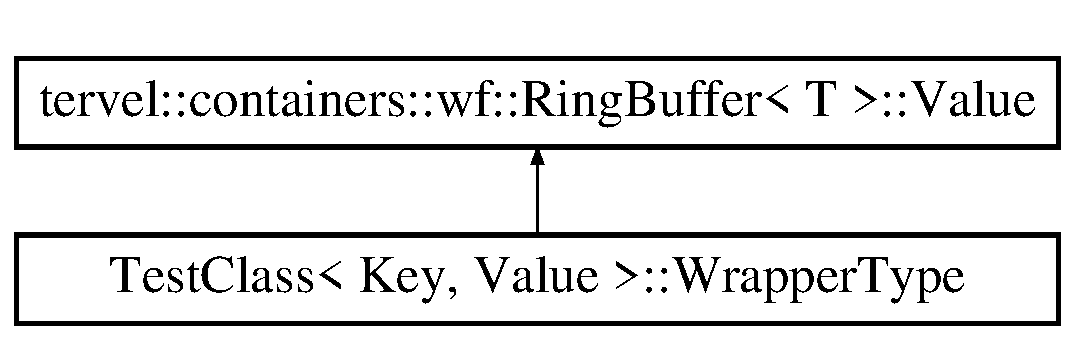
\includegraphics[height=2.000000cm]{classtervel_1_1containers_1_1wf_1_1_ring_buffer_1_1_value}
\end{center}
\end{figure}
\subsection*{Public Member Functions}
\begin{DoxyCompactItemize}
\item 
\hyperlink{classtervel_1_1containers_1_1wf_1_1_ring_buffer_1_1_value_a613688460de05951b79f31a3f1482ede}{Value} ()
\begin{DoxyCompactList}\small\item\em Empty constructor. \end{DoxyCompactList}\end{DoxyCompactItemize}
\subsection*{Public Attributes}
\begin{DoxyCompactItemize}
\item 
friend \hyperlink{classtervel_1_1containers_1_1wf_1_1_ring_buffer_1_1_value_a603884ee3e254094da695fa05b796764}{Ring\+Buffer}
\end{DoxyCompactItemize}
\subsection*{Private Member Functions}
\begin{DoxyCompactItemize}
\item 
int64\+\_\+t \hyperlink{classtervel_1_1containers_1_1wf_1_1_ring_buffer_1_1_value_addbad0a38025643a16f01edaf501a982}{func\+\_\+seqid} ()
\begin{DoxyCompactList}\small\item\em Returns the items seqid. \end{DoxyCompactList}\item 
void \hyperlink{classtervel_1_1containers_1_1wf_1_1_ring_buffer_1_1_value_a1ea5c365921ff3476b5dba84ad104cbc}{func\+\_\+seqid} (int64\+\_\+t s)
\begin{DoxyCompactList}\small\item\em Sets the items seqid. \end{DoxyCompactList}\item 
void \hyperlink{classtervel_1_1containers_1_1wf_1_1_ring_buffer_1_1_value_a7bd2fbc2b8577ac6bd884e06328bfb2d}{atomic\+\_\+change\+\_\+seqid} (int64\+\_\+t e, int64\+\_\+t n)
\begin{DoxyCompactList}\small\item\em Conditionally updates the seqid. \end{DoxyCompactList}\end{DoxyCompactItemize}
\subsection*{Private Attributes}
\begin{DoxyCompactItemize}
\item 
int64\+\_\+t \hyperlink{classtervel_1_1containers_1_1wf_1_1_ring_buffer_1_1_value_aaecdcc3fbb8c5a8b784625e835c7d6ef}{seqid\+\_\+} \{-\/1\}
\end{DoxyCompactItemize}


\subsection{Detailed Description}
\subsubsection*{template$<$typename T$>$class tervel\+::containers\+::wf\+::\+Ring\+Buffer$<$ T $>$\+::\+Value}

\hyperlink{classtervel_1_1containers_1_1wf_1_1_ring_buffer}{Ring\+Buffer} value class, values stored in the class must extend it. 

This class is necessary to provide the F\+I\+F\+O property. It adds a sequence identifier to each value stored. Using this identifier, we are apply generate F\+I\+F\+O valid sequential history from a concurrent history. 

\subsection{Constructor \& Destructor Documentation}
\hypertarget{classtervel_1_1containers_1_1wf_1_1_ring_buffer_1_1_value_a613688460de05951b79f31a3f1482ede}{}\index{tervel\+::containers\+::wf\+::\+Ring\+Buffer\+::\+Value@{tervel\+::containers\+::wf\+::\+Ring\+Buffer\+::\+Value}!Value@{Value}}
\index{Value@{Value}!tervel\+::containers\+::wf\+::\+Ring\+Buffer\+::\+Value@{tervel\+::containers\+::wf\+::\+Ring\+Buffer\+::\+Value}}
\subsubsection[{Value()}]{\setlength{\rightskip}{0pt plus 5cm}template$<$typename T$>$ {\bf tervel\+::containers\+::wf\+::\+Ring\+Buffer}$<$ T $>$\+::Value\+::\+Value (
\begin{DoxyParamCaption}
{}
\end{DoxyParamCaption}
)\hspace{0.3cm}{\ttfamily [inline]}}\label{classtervel_1_1containers_1_1wf_1_1_ring_buffer_1_1_value_a613688460de05951b79f31a3f1482ede}


Empty constructor. 

Empty Constructor 

\subsection{Member Function Documentation}
\hypertarget{classtervel_1_1containers_1_1wf_1_1_ring_buffer_1_1_value_a7bd2fbc2b8577ac6bd884e06328bfb2d}{}\index{tervel\+::containers\+::wf\+::\+Ring\+Buffer\+::\+Value@{tervel\+::containers\+::wf\+::\+Ring\+Buffer\+::\+Value}!atomic\+\_\+change\+\_\+seqid@{atomic\+\_\+change\+\_\+seqid}}
\index{atomic\+\_\+change\+\_\+seqid@{atomic\+\_\+change\+\_\+seqid}!tervel\+::containers\+::wf\+::\+Ring\+Buffer\+::\+Value@{tervel\+::containers\+::wf\+::\+Ring\+Buffer\+::\+Value}}
\subsubsection[{atomic\+\_\+change\+\_\+seqid(int64\+\_\+t e, int64\+\_\+t n)}]{\setlength{\rightskip}{0pt plus 5cm}template$<$typename T$>$ void {\bf tervel\+::containers\+::wf\+::\+Ring\+Buffer}$<$ T $>$\+::Value\+::atomic\+\_\+change\+\_\+seqid (
\begin{DoxyParamCaption}
\item[{int64\+\_\+t}]{e, }
\item[{int64\+\_\+t}]{n}
\end{DoxyParamCaption}
)\hspace{0.3cm}{\ttfamily [inline]}, {\ttfamily [private]}}\label{classtervel_1_1containers_1_1wf_1_1_ring_buffer_1_1_value_a7bd2fbc2b8577ac6bd884e06328bfb2d}


Conditionally updates the seqid. 

This function is used when multiple threads maybe enqueueing the same value


\begin{DoxyParams}{Parameters}
{\em e} & expected seqid (address of the oprec $\ast$ -\/1). \\
\hline
{\em n} & new seqid \\
\hline
\end{DoxyParams}
\hypertarget{classtervel_1_1containers_1_1wf_1_1_ring_buffer_1_1_value_addbad0a38025643a16f01edaf501a982}{}\index{tervel\+::containers\+::wf\+::\+Ring\+Buffer\+::\+Value@{tervel\+::containers\+::wf\+::\+Ring\+Buffer\+::\+Value}!func\+\_\+seqid@{func\+\_\+seqid}}
\index{func\+\_\+seqid@{func\+\_\+seqid}!tervel\+::containers\+::wf\+::\+Ring\+Buffer\+::\+Value@{tervel\+::containers\+::wf\+::\+Ring\+Buffer\+::\+Value}}
\subsubsection[{func\+\_\+seqid()}]{\setlength{\rightskip}{0pt plus 5cm}template$<$typename T$>$ int64\+\_\+t {\bf tervel\+::containers\+::wf\+::\+Ring\+Buffer}$<$ T $>$\+::Value\+::func\+\_\+seqid (
\begin{DoxyParamCaption}
{}
\end{DoxyParamCaption}
)\hspace{0.3cm}{\ttfamily [inline]}, {\ttfamily [private]}}\label{classtervel_1_1containers_1_1wf_1_1_ring_buffer_1_1_value_addbad0a38025643a16f01edaf501a982}


Returns the items seqid. 

Returns the items seqid \begin{DoxyReturn}{Returns}
Returns the items seqid 
\end{DoxyReturn}
\hypertarget{classtervel_1_1containers_1_1wf_1_1_ring_buffer_1_1_value_a1ea5c365921ff3476b5dba84ad104cbc}{}\index{tervel\+::containers\+::wf\+::\+Ring\+Buffer\+::\+Value@{tervel\+::containers\+::wf\+::\+Ring\+Buffer\+::\+Value}!func\+\_\+seqid@{func\+\_\+seqid}}
\index{func\+\_\+seqid@{func\+\_\+seqid}!tervel\+::containers\+::wf\+::\+Ring\+Buffer\+::\+Value@{tervel\+::containers\+::wf\+::\+Ring\+Buffer\+::\+Value}}
\subsubsection[{func\+\_\+seqid(int64\+\_\+t s)}]{\setlength{\rightskip}{0pt plus 5cm}template$<$typename T$>$ void {\bf tervel\+::containers\+::wf\+::\+Ring\+Buffer}$<$ T $>$\+::Value\+::func\+\_\+seqid (
\begin{DoxyParamCaption}
\item[{int64\+\_\+t}]{s}
\end{DoxyParamCaption}
)\hspace{0.3cm}{\ttfamily [inline]}, {\ttfamily [private]}}\label{classtervel_1_1containers_1_1wf_1_1_ring_buffer_1_1_value_a1ea5c365921ff3476b5dba84ad104cbc}


Sets the items seqid. 

Sets the items seqid \begin{DoxyReturn}{Returns}
Sets the items seqid 
\end{DoxyReturn}


\subsection{Member Data Documentation}
\hypertarget{classtervel_1_1containers_1_1wf_1_1_ring_buffer_1_1_value_a603884ee3e254094da695fa05b796764}{}\index{tervel\+::containers\+::wf\+::\+Ring\+Buffer\+::\+Value@{tervel\+::containers\+::wf\+::\+Ring\+Buffer\+::\+Value}!Ring\+Buffer@{Ring\+Buffer}}
\index{Ring\+Buffer@{Ring\+Buffer}!tervel\+::containers\+::wf\+::\+Ring\+Buffer\+::\+Value@{tervel\+::containers\+::wf\+::\+Ring\+Buffer\+::\+Value}}
\subsubsection[{Ring\+Buffer}]{\setlength{\rightskip}{0pt plus 5cm}template$<$typename T$>$ friend {\bf tervel\+::containers\+::wf\+::\+Ring\+Buffer}$<$ T $>$\+::Value\+::\+Ring\+Buffer}\label{classtervel_1_1containers_1_1wf_1_1_ring_buffer_1_1_value_a603884ee3e254094da695fa05b796764}
\hypertarget{classtervel_1_1containers_1_1wf_1_1_ring_buffer_1_1_value_aaecdcc3fbb8c5a8b784625e835c7d6ef}{}\index{tervel\+::containers\+::wf\+::\+Ring\+Buffer\+::\+Value@{tervel\+::containers\+::wf\+::\+Ring\+Buffer\+::\+Value}!seqid\+\_\+@{seqid\+\_\+}}
\index{seqid\+\_\+@{seqid\+\_\+}!tervel\+::containers\+::wf\+::\+Ring\+Buffer\+::\+Value@{tervel\+::containers\+::wf\+::\+Ring\+Buffer\+::\+Value}}
\subsubsection[{seqid\+\_\+}]{\setlength{\rightskip}{0pt plus 5cm}template$<$typename T$>$ int64\+\_\+t {\bf tervel\+::containers\+::wf\+::\+Ring\+Buffer}$<$ T $>$\+::Value\+::seqid\+\_\+ \{-\/1\}\hspace{0.3cm}{\ttfamily [private]}}\label{classtervel_1_1containers_1_1wf_1_1_ring_buffer_1_1_value_aaecdcc3fbb8c5a8b784625e835c7d6ef}


The documentation for this class was generated from the following file\+:\begin{DoxyCompactItemize}
\item 
tervel/containers/wf/ring-\/buffer/\hyperlink{ring__buffer_8h}{ring\+\_\+buffer.\+h}\end{DoxyCompactItemize}

\hypertarget{classtervel_1_1containers_1_1wf_1_1_hash_map_1_1_value_accessor}{}\section{tervel\+:\+:containers\+:\+:wf\+:\+:Hash\+Map$<$ Key, Value, Functor $>$\+:\+:Value\+Accessor Class Reference}
\label{classtervel_1_1containers_1_1wf_1_1_hash_map_1_1_value_accessor}\index{tervel\+::containers\+::wf\+::\+Hash\+Map$<$ Key, Value, Functor $>$\+::\+Value\+Accessor@{tervel\+::containers\+::wf\+::\+Hash\+Map$<$ Key, Value, Functor $>$\+::\+Value\+Accessor}}


This class is used to safe guard access to values.  




{\ttfamily \#include $<$wf\+\_\+hash\+\_\+map.\+h$>$}

\subsection*{Public Member Functions}
\begin{DoxyCompactItemize}
\item 
\hyperlink{classtervel_1_1containers_1_1wf_1_1_hash_map_1_1_value_accessor_a5cf5be9f8fcf0b32ecac2d6ba1d18a24}{Value\+Accessor} ()
\item 
\hyperlink{classtervel_1_1containers_1_1wf_1_1_hash_map_1_1_value_accessor_a4a79d0ccc099187188e7d001406f4381}{$\sim$\+Value\+Accessor} ()
\item 
\hyperlink{hash__map_2test_object_8h_ad777bf08d8e2b01df17ba5e3c51ae11f}{Value} $\ast$ \hyperlink{classtervel_1_1containers_1_1wf_1_1_hash_map_1_1_value_accessor_a54f9f278457daf02a4e140cbe053643b}{value} ()
\item 
bool \hyperlink{classtervel_1_1containers_1_1wf_1_1_hash_map_1_1_value_accessor_adf525344b84c57e6c560b7fe46db7a4f}{valid} ()
\item 
void \hyperlink{classtervel_1_1containers_1_1wf_1_1_hash_map_1_1_value_accessor_ac255a8bda6d5118c2987f91aa4cc0ca7}{reset} ()
\begin{DoxyCompactList}\small\item\em Resets this value accessors, decrementing the access\+\_\+count and clearing the variables. \end{DoxyCompactList}\end{DoxyCompactItemize}
\subsection*{Private Member Functions}
\begin{DoxyCompactItemize}
\item 
void \hyperlink{classtervel_1_1containers_1_1wf_1_1_hash_map_1_1_value_accessor_a44db31fa9f2364a0dddf193dcd3e0c72}{init} (\hyperlink{hash__map_2test_object_8h_ad777bf08d8e2b01df17ba5e3c51ae11f}{Value} $\ast$\hyperlink{classtervel_1_1containers_1_1wf_1_1_hash_map_1_1_value_accessor_a54f9f278457daf02a4e140cbe053643b}{value}, std\+::atomic$<$ int64\+\_\+t $>$ $\ast$access\+\_\+count)
\begin{DoxyCompactList}\small\item\em Initializes the value accessor. \end{DoxyCompactList}\end{DoxyCompactItemize}
\subsection*{Private Attributes}
\begin{DoxyCompactItemize}
\item 
std\+::atomic$<$ int64\+\_\+t $>$ $\ast$ \hyperlink{classtervel_1_1containers_1_1wf_1_1_hash_map_1_1_value_accessor_a618a0a94c509bc451fd63cf0687ca527}{access\+\_\+count\+\_\+}
\item 
\hyperlink{hash__map_2test_object_8h_ad777bf08d8e2b01df17ba5e3c51ae11f}{Value} $\ast$ \hyperlink{classtervel_1_1containers_1_1wf_1_1_hash_map_1_1_value_accessor_a75ab81c8fa2032a5a4a9dff43227c387}{value\+\_\+}
\end{DoxyCompactItemize}
\subsection*{Friends}
\begin{DoxyCompactItemize}
\item 
class \hyperlink{classtervel_1_1containers_1_1wf_1_1_hash_map_1_1_value_accessor_ab6054287e6f409207af3fa16e49046ad}{Hash\+Map}
\end{DoxyCompactItemize}


\subsection{Detailed Description}
\subsubsection*{template$<$class Key, class Value, class Functor = default\+\_\+functor$<$\+Key, Value$>$$>$class tervel\+::containers\+::wf\+::\+Hash\+Map$<$ Key, Value, Functor $>$\+::\+Value\+Accessor}

This class is used to safe guard access to values. 

Before it is initialized the referenced data\+\_\+node\textquotesingle{}s access counter would have been incremented. 

\subsection{Constructor \& Destructor Documentation}
\hypertarget{classtervel_1_1containers_1_1wf_1_1_hash_map_1_1_value_accessor_a5cf5be9f8fcf0b32ecac2d6ba1d18a24}{}\index{tervel\+::containers\+::wf\+::\+Hash\+Map\+::\+Value\+Accessor@{tervel\+::containers\+::wf\+::\+Hash\+Map\+::\+Value\+Accessor}!Value\+Accessor@{Value\+Accessor}}
\index{Value\+Accessor@{Value\+Accessor}!tervel\+::containers\+::wf\+::\+Hash\+Map\+::\+Value\+Accessor@{tervel\+::containers\+::wf\+::\+Hash\+Map\+::\+Value\+Accessor}}
\subsubsection[{Value\+Accessor()}]{\setlength{\rightskip}{0pt plus 5cm}template$<$class Key , class Value , class Functor  = default\+\_\+functor$<$\+Key, Value$>$$>$ {\bf tervel\+::containers\+::wf\+::\+Hash\+Map}$<$ Key, {\bf Value}, Functor $>$\+::Value\+Accessor\+::\+Value\+Accessor (
\begin{DoxyParamCaption}
{}
\end{DoxyParamCaption}
)\hspace{0.3cm}{\ttfamily [inline]}}\label{classtervel_1_1containers_1_1wf_1_1_hash_map_1_1_value_accessor_a5cf5be9f8fcf0b32ecac2d6ba1d18a24}
\hypertarget{classtervel_1_1containers_1_1wf_1_1_hash_map_1_1_value_accessor_a4a79d0ccc099187188e7d001406f4381}{}\index{tervel\+::containers\+::wf\+::\+Hash\+Map\+::\+Value\+Accessor@{tervel\+::containers\+::wf\+::\+Hash\+Map\+::\+Value\+Accessor}!````~Value\+Accessor@{$\sim$\+Value\+Accessor}}
\index{````~Value\+Accessor@{$\sim$\+Value\+Accessor}!tervel\+::containers\+::wf\+::\+Hash\+Map\+::\+Value\+Accessor@{tervel\+::containers\+::wf\+::\+Hash\+Map\+::\+Value\+Accessor}}
\subsubsection[{$\sim$\+Value\+Accessor()}]{\setlength{\rightskip}{0pt plus 5cm}template$<$class Key , class Value , class Functor  = default\+\_\+functor$<$\+Key, Value$>$$>$ {\bf tervel\+::containers\+::wf\+::\+Hash\+Map}$<$ Key, {\bf Value}, Functor $>$\+::Value\+Accessor\+::$\sim$\+Value\+Accessor (
\begin{DoxyParamCaption}
{}
\end{DoxyParamCaption}
)\hspace{0.3cm}{\ttfamily [inline]}}\label{classtervel_1_1containers_1_1wf_1_1_hash_map_1_1_value_accessor_a4a79d0ccc099187188e7d001406f4381}


\subsection{Member Function Documentation}
\hypertarget{classtervel_1_1containers_1_1wf_1_1_hash_map_1_1_value_accessor_a44db31fa9f2364a0dddf193dcd3e0c72}{}\index{tervel\+::containers\+::wf\+::\+Hash\+Map\+::\+Value\+Accessor@{tervel\+::containers\+::wf\+::\+Hash\+Map\+::\+Value\+Accessor}!init@{init}}
\index{init@{init}!tervel\+::containers\+::wf\+::\+Hash\+Map\+::\+Value\+Accessor@{tervel\+::containers\+::wf\+::\+Hash\+Map\+::\+Value\+Accessor}}
\subsubsection[{init(\+Value $\ast$value, std\+::atomic$<$ int64\+\_\+t $>$ $\ast$access\+\_\+count)}]{\setlength{\rightskip}{0pt plus 5cm}template$<$class Key , class Value , class Functor  = default\+\_\+functor$<$\+Key, Value$>$$>$ void {\bf tervel\+::containers\+::wf\+::\+Hash\+Map}$<$ Key, {\bf Value}, Functor $>$\+::Value\+Accessor\+::init (
\begin{DoxyParamCaption}
\item[{{\bf Value} $\ast$}]{value, }
\item[{std\+::atomic$<$ int64\+\_\+t $>$ $\ast$}]{access\+\_\+count}
\end{DoxyParamCaption}
)\hspace{0.3cm}{\ttfamily [inline]}, {\ttfamily [private]}}\label{classtervel_1_1containers_1_1wf_1_1_hash_map_1_1_value_accessor_a44db31fa9f2364a0dddf193dcd3e0c72}


Initializes the value accessor. 


\begin{DoxyParams}{Parameters}
{\em value} & the address of the value \\
\hline
{\em access\+\_\+count} & the address of the value\textquotesingle{}s access\+\_\+count \\
\hline
\end{DoxyParams}
\hypertarget{classtervel_1_1containers_1_1wf_1_1_hash_map_1_1_value_accessor_ac255a8bda6d5118c2987f91aa4cc0ca7}{}\index{tervel\+::containers\+::wf\+::\+Hash\+Map\+::\+Value\+Accessor@{tervel\+::containers\+::wf\+::\+Hash\+Map\+::\+Value\+Accessor}!reset@{reset}}
\index{reset@{reset}!tervel\+::containers\+::wf\+::\+Hash\+Map\+::\+Value\+Accessor@{tervel\+::containers\+::wf\+::\+Hash\+Map\+::\+Value\+Accessor}}
\subsubsection[{reset()}]{\setlength{\rightskip}{0pt plus 5cm}template$<$class Key , class Value , class Functor  = default\+\_\+functor$<$\+Key, Value$>$$>$ void {\bf tervel\+::containers\+::wf\+::\+Hash\+Map}$<$ Key, {\bf Value}, Functor $>$\+::Value\+Accessor\+::reset (
\begin{DoxyParamCaption}
{}
\end{DoxyParamCaption}
)\hspace{0.3cm}{\ttfamily [inline]}}\label{classtervel_1_1containers_1_1wf_1_1_hash_map_1_1_value_accessor_ac255a8bda6d5118c2987f91aa4cc0ca7}


Resets this value accessors, decrementing the access\+\_\+count and clearing the variables. 

\hypertarget{classtervel_1_1containers_1_1wf_1_1_hash_map_1_1_value_accessor_adf525344b84c57e6c560b7fe46db7a4f}{}\index{tervel\+::containers\+::wf\+::\+Hash\+Map\+::\+Value\+Accessor@{tervel\+::containers\+::wf\+::\+Hash\+Map\+::\+Value\+Accessor}!valid@{valid}}
\index{valid@{valid}!tervel\+::containers\+::wf\+::\+Hash\+Map\+::\+Value\+Accessor@{tervel\+::containers\+::wf\+::\+Hash\+Map\+::\+Value\+Accessor}}
\subsubsection[{valid()}]{\setlength{\rightskip}{0pt plus 5cm}template$<$class Key , class Value , class Functor  = default\+\_\+functor$<$\+Key, Value$>$$>$ bool {\bf tervel\+::containers\+::wf\+::\+Hash\+Map}$<$ Key, {\bf Value}, Functor $>$\+::Value\+Accessor\+::valid (
\begin{DoxyParamCaption}
{}
\end{DoxyParamCaption}
)\hspace{0.3cm}{\ttfamily [inline]}}\label{classtervel_1_1containers_1_1wf_1_1_hash_map_1_1_value_accessor_adf525344b84c57e6c560b7fe46db7a4f}
\begin{DoxyReturn}{Returns}
whether or not this was initialized. 
\end{DoxyReturn}
\hypertarget{classtervel_1_1containers_1_1wf_1_1_hash_map_1_1_value_accessor_a54f9f278457daf02a4e140cbe053643b}{}\index{tervel\+::containers\+::wf\+::\+Hash\+Map\+::\+Value\+Accessor@{tervel\+::containers\+::wf\+::\+Hash\+Map\+::\+Value\+Accessor}!value@{value}}
\index{value@{value}!tervel\+::containers\+::wf\+::\+Hash\+Map\+::\+Value\+Accessor@{tervel\+::containers\+::wf\+::\+Hash\+Map\+::\+Value\+Accessor}}
\subsubsection[{value()}]{\setlength{\rightskip}{0pt plus 5cm}template$<$class Key , class Value , class Functor  = default\+\_\+functor$<$\+Key, Value$>$$>$ {\bf Value}$\ast$ {\bf tervel\+::containers\+::wf\+::\+Hash\+Map}$<$ Key, {\bf Value}, Functor $>$\+::Value\+Accessor\+::value (
\begin{DoxyParamCaption}
{}
\end{DoxyParamCaption}
)\hspace{0.3cm}{\ttfamily [inline]}}\label{classtervel_1_1containers_1_1wf_1_1_hash_map_1_1_value_accessor_a54f9f278457daf02a4e140cbe053643b}
\begin{DoxyReturn}{Returns}
the address of the value in the data\+\_\+node. 
\end{DoxyReturn}


\subsection{Friends And Related Function Documentation}
\hypertarget{classtervel_1_1containers_1_1wf_1_1_hash_map_1_1_value_accessor_ab6054287e6f409207af3fa16e49046ad}{}\index{tervel\+::containers\+::wf\+::\+Hash\+Map\+::\+Value\+Accessor@{tervel\+::containers\+::wf\+::\+Hash\+Map\+::\+Value\+Accessor}!Hash\+Map@{Hash\+Map}}
\index{Hash\+Map@{Hash\+Map}!tervel\+::containers\+::wf\+::\+Hash\+Map\+::\+Value\+Accessor@{tervel\+::containers\+::wf\+::\+Hash\+Map\+::\+Value\+Accessor}}
\subsubsection[{Hash\+Map}]{\setlength{\rightskip}{0pt plus 5cm}template$<$class Key , class Value , class Functor  = default\+\_\+functor$<$\+Key, Value$>$$>$ friend class {\bf Hash\+Map}\hspace{0.3cm}{\ttfamily [friend]}}\label{classtervel_1_1containers_1_1wf_1_1_hash_map_1_1_value_accessor_ab6054287e6f409207af3fa16e49046ad}


\subsection{Member Data Documentation}
\hypertarget{classtervel_1_1containers_1_1wf_1_1_hash_map_1_1_value_accessor_a618a0a94c509bc451fd63cf0687ca527}{}\index{tervel\+::containers\+::wf\+::\+Hash\+Map\+::\+Value\+Accessor@{tervel\+::containers\+::wf\+::\+Hash\+Map\+::\+Value\+Accessor}!access\+\_\+count\+\_\+@{access\+\_\+count\+\_\+}}
\index{access\+\_\+count\+\_\+@{access\+\_\+count\+\_\+}!tervel\+::containers\+::wf\+::\+Hash\+Map\+::\+Value\+Accessor@{tervel\+::containers\+::wf\+::\+Hash\+Map\+::\+Value\+Accessor}}
\subsubsection[{access\+\_\+count\+\_\+}]{\setlength{\rightskip}{0pt plus 5cm}template$<$class Key , class Value , class Functor  = default\+\_\+functor$<$\+Key, Value$>$$>$ std\+::atomic$<$int64\+\_\+t$>$$\ast$ {\bf tervel\+::containers\+::wf\+::\+Hash\+Map}$<$ Key, {\bf Value}, Functor $>$\+::Value\+Accessor\+::access\+\_\+count\+\_\+\hspace{0.3cm}{\ttfamily [private]}}\label{classtervel_1_1containers_1_1wf_1_1_hash_map_1_1_value_accessor_a618a0a94c509bc451fd63cf0687ca527}
\hypertarget{classtervel_1_1containers_1_1wf_1_1_hash_map_1_1_value_accessor_a75ab81c8fa2032a5a4a9dff43227c387}{}\index{tervel\+::containers\+::wf\+::\+Hash\+Map\+::\+Value\+Accessor@{tervel\+::containers\+::wf\+::\+Hash\+Map\+::\+Value\+Accessor}!value\+\_\+@{value\+\_\+}}
\index{value\+\_\+@{value\+\_\+}!tervel\+::containers\+::wf\+::\+Hash\+Map\+::\+Value\+Accessor@{tervel\+::containers\+::wf\+::\+Hash\+Map\+::\+Value\+Accessor}}
\subsubsection[{value\+\_\+}]{\setlength{\rightskip}{0pt plus 5cm}template$<$class Key , class Value , class Functor  = default\+\_\+functor$<$\+Key, Value$>$$>$ {\bf Value}$\ast$ {\bf tervel\+::containers\+::wf\+::\+Hash\+Map}$<$ Key, {\bf Value}, Functor $>$\+::Value\+Accessor\+::value\+\_\+\hspace{0.3cm}{\ttfamily [private]}}\label{classtervel_1_1containers_1_1wf_1_1_hash_map_1_1_value_accessor_a75ab81c8fa2032a5a4a9dff43227c387}


The documentation for this class was generated from the following file\+:\begin{DoxyCompactItemize}
\item 
tervel/containers/wf/hash-\/map/\hyperlink{wf__hash__map_8h}{wf\+\_\+hash\+\_\+map.\+h}\end{DoxyCompactItemize}

\hypertarget{classtervel_1_1containers_1_1wf_1_1_hash_map_no_delete_1_1_value_accessor}{}\section{tervel\+:\+:containers\+:\+:wf\+:\+:Hash\+Map\+No\+Delete$<$ Key, Value, Functor $>$\+:\+:Value\+Accessor Class Reference}
\label{classtervel_1_1containers_1_1wf_1_1_hash_map_no_delete_1_1_value_accessor}\index{tervel\+::containers\+::wf\+::\+Hash\+Map\+No\+Delete$<$ Key, Value, Functor $>$\+::\+Value\+Accessor@{tervel\+::containers\+::wf\+::\+Hash\+Map\+No\+Delete$<$ Key, Value, Functor $>$\+::\+Value\+Accessor}}


This class is used to safe guard access to values.  




{\ttfamily \#include $<$wf\+\_\+hash\+\_\+map\+\_\+no\+\_\+delete.\+h$>$}

\subsection*{Public Member Functions}
\begin{DoxyCompactItemize}
\item 
\hyperlink{classtervel_1_1containers_1_1wf_1_1_hash_map_no_delete_1_1_value_accessor_a17de96d4fed12a69e2647d5bd34a5ff8}{Value\+Accessor} ()
\item 
\hyperlink{classtervel_1_1containers_1_1wf_1_1_hash_map_no_delete_1_1_value_accessor_a210c575aeca4a00804b78af1200c05c4}{$\sim$\+Value\+Accessor} ()
\item 
\hyperlink{hash__map_2test_object_8h_ad777bf08d8e2b01df17ba5e3c51ae11f}{Value} $\ast$ \hyperlink{classtervel_1_1containers_1_1wf_1_1_hash_map_no_delete_1_1_value_accessor_acf5a7975064652eacc15c034fe6391b6}{value} ()
\item 
bool \hyperlink{classtervel_1_1containers_1_1wf_1_1_hash_map_no_delete_1_1_value_accessor_aa0a24d417644c8967086d1c80a3e6554}{valid} ()
\item 
void \hyperlink{classtervel_1_1containers_1_1wf_1_1_hash_map_no_delete_1_1_value_accessor_aa1e3978b97fda613c947ec71147dcbee}{reset} ()
\begin{DoxyCompactList}\small\item\em Resets this value accessors,clearing the variables. \end{DoxyCompactList}\end{DoxyCompactItemize}
\subsection*{Private Member Functions}
\begin{DoxyCompactItemize}
\item 
void \hyperlink{classtervel_1_1containers_1_1wf_1_1_hash_map_no_delete_1_1_value_accessor_aacf538df718d0e496336ff3a11290c9b}{init} (\hyperlink{hash__map_2test_object_8h_ad777bf08d8e2b01df17ba5e3c51ae11f}{Value} $\ast$\hyperlink{classtervel_1_1containers_1_1wf_1_1_hash_map_no_delete_1_1_value_accessor_acf5a7975064652eacc15c034fe6391b6}{value})
\begin{DoxyCompactList}\small\item\em Initializes the value accessors. \end{DoxyCompactList}\end{DoxyCompactItemize}
\subsection*{Private Attributes}
\begin{DoxyCompactItemize}
\item 
\hyperlink{hash__map_2test_object_8h_ad777bf08d8e2b01df17ba5e3c51ae11f}{Value} $\ast$ \hyperlink{classtervel_1_1containers_1_1wf_1_1_hash_map_no_delete_1_1_value_accessor_a5e4972255abbbd6ae7ff8d7f15d6ff67}{value\+\_\+}
\end{DoxyCompactItemize}
\subsection*{Friends}
\begin{DoxyCompactItemize}
\item 
class \hyperlink{classtervel_1_1containers_1_1wf_1_1_hash_map_no_delete_1_1_value_accessor_a8a4142949547f715390cedfd99659a85}{Hash\+Map\+No\+Delete}
\end{DoxyCompactItemize}


\subsection{Detailed Description}
\subsubsection*{template$<$class Key, class Value, class Functor = default\+\_\+functor$<$\+Key, Value$>$$>$class tervel\+::containers\+::wf\+::\+Hash\+Map\+No\+Delete$<$ Key, Value, Functor $>$\+::\+Value\+Accessor}

This class is used to safe guard access to values. 

\subsection{Constructor \& Destructor Documentation}
\hypertarget{classtervel_1_1containers_1_1wf_1_1_hash_map_no_delete_1_1_value_accessor_a17de96d4fed12a69e2647d5bd34a5ff8}{}\index{tervel\+::containers\+::wf\+::\+Hash\+Map\+No\+Delete\+::\+Value\+Accessor@{tervel\+::containers\+::wf\+::\+Hash\+Map\+No\+Delete\+::\+Value\+Accessor}!Value\+Accessor@{Value\+Accessor}}
\index{Value\+Accessor@{Value\+Accessor}!tervel\+::containers\+::wf\+::\+Hash\+Map\+No\+Delete\+::\+Value\+Accessor@{tervel\+::containers\+::wf\+::\+Hash\+Map\+No\+Delete\+::\+Value\+Accessor}}
\subsubsection[{Value\+Accessor()}]{\setlength{\rightskip}{0pt plus 5cm}template$<$class Key , class Value , class Functor  = default\+\_\+functor$<$\+Key, Value$>$$>$ {\bf tervel\+::containers\+::wf\+::\+Hash\+Map\+No\+Delete}$<$ Key, {\bf Value}, Functor $>$\+::Value\+Accessor\+::\+Value\+Accessor (
\begin{DoxyParamCaption}
{}
\end{DoxyParamCaption}
)\hspace{0.3cm}{\ttfamily [inline]}}\label{classtervel_1_1containers_1_1wf_1_1_hash_map_no_delete_1_1_value_accessor_a17de96d4fed12a69e2647d5bd34a5ff8}
\hypertarget{classtervel_1_1containers_1_1wf_1_1_hash_map_no_delete_1_1_value_accessor_a210c575aeca4a00804b78af1200c05c4}{}\index{tervel\+::containers\+::wf\+::\+Hash\+Map\+No\+Delete\+::\+Value\+Accessor@{tervel\+::containers\+::wf\+::\+Hash\+Map\+No\+Delete\+::\+Value\+Accessor}!````~Value\+Accessor@{$\sim$\+Value\+Accessor}}
\index{````~Value\+Accessor@{$\sim$\+Value\+Accessor}!tervel\+::containers\+::wf\+::\+Hash\+Map\+No\+Delete\+::\+Value\+Accessor@{tervel\+::containers\+::wf\+::\+Hash\+Map\+No\+Delete\+::\+Value\+Accessor}}
\subsubsection[{$\sim$\+Value\+Accessor()}]{\setlength{\rightskip}{0pt plus 5cm}template$<$class Key , class Value , class Functor  = default\+\_\+functor$<$\+Key, Value$>$$>$ {\bf tervel\+::containers\+::wf\+::\+Hash\+Map\+No\+Delete}$<$ Key, {\bf Value}, Functor $>$\+::Value\+Accessor\+::$\sim$\+Value\+Accessor (
\begin{DoxyParamCaption}
{}
\end{DoxyParamCaption}
)\hspace{0.3cm}{\ttfamily [inline]}}\label{classtervel_1_1containers_1_1wf_1_1_hash_map_no_delete_1_1_value_accessor_a210c575aeca4a00804b78af1200c05c4}


\subsection{Member Function Documentation}
\hypertarget{classtervel_1_1containers_1_1wf_1_1_hash_map_no_delete_1_1_value_accessor_aacf538df718d0e496336ff3a11290c9b}{}\index{tervel\+::containers\+::wf\+::\+Hash\+Map\+No\+Delete\+::\+Value\+Accessor@{tervel\+::containers\+::wf\+::\+Hash\+Map\+No\+Delete\+::\+Value\+Accessor}!init@{init}}
\index{init@{init}!tervel\+::containers\+::wf\+::\+Hash\+Map\+No\+Delete\+::\+Value\+Accessor@{tervel\+::containers\+::wf\+::\+Hash\+Map\+No\+Delete\+::\+Value\+Accessor}}
\subsubsection[{init(\+Value $\ast$value)}]{\setlength{\rightskip}{0pt plus 5cm}template$<$class Key , class Value , class Functor  = default\+\_\+functor$<$\+Key, Value$>$$>$ void {\bf tervel\+::containers\+::wf\+::\+Hash\+Map\+No\+Delete}$<$ Key, {\bf Value}, Functor $>$\+::Value\+Accessor\+::init (
\begin{DoxyParamCaption}
\item[{{\bf Value} $\ast$}]{value}
\end{DoxyParamCaption}
)\hspace{0.3cm}{\ttfamily [inline]}, {\ttfamily [private]}}\label{classtervel_1_1containers_1_1wf_1_1_hash_map_no_delete_1_1_value_accessor_aacf538df718d0e496336ff3a11290c9b}


Initializes the value accessors. 


\begin{DoxyParams}{Parameters}
{\em value} & the address of the value \\
\hline
\end{DoxyParams}
\hypertarget{classtervel_1_1containers_1_1wf_1_1_hash_map_no_delete_1_1_value_accessor_aa1e3978b97fda613c947ec71147dcbee}{}\index{tervel\+::containers\+::wf\+::\+Hash\+Map\+No\+Delete\+::\+Value\+Accessor@{tervel\+::containers\+::wf\+::\+Hash\+Map\+No\+Delete\+::\+Value\+Accessor}!reset@{reset}}
\index{reset@{reset}!tervel\+::containers\+::wf\+::\+Hash\+Map\+No\+Delete\+::\+Value\+Accessor@{tervel\+::containers\+::wf\+::\+Hash\+Map\+No\+Delete\+::\+Value\+Accessor}}
\subsubsection[{reset()}]{\setlength{\rightskip}{0pt plus 5cm}template$<$class Key , class Value , class Functor  = default\+\_\+functor$<$\+Key, Value$>$$>$ void {\bf tervel\+::containers\+::wf\+::\+Hash\+Map\+No\+Delete}$<$ Key, {\bf Value}, Functor $>$\+::Value\+Accessor\+::reset (
\begin{DoxyParamCaption}
{}
\end{DoxyParamCaption}
)\hspace{0.3cm}{\ttfamily [inline]}}\label{classtervel_1_1containers_1_1wf_1_1_hash_map_no_delete_1_1_value_accessor_aa1e3978b97fda613c947ec71147dcbee}


Resets this value accessors,clearing the variables. 

\hypertarget{classtervel_1_1containers_1_1wf_1_1_hash_map_no_delete_1_1_value_accessor_aa0a24d417644c8967086d1c80a3e6554}{}\index{tervel\+::containers\+::wf\+::\+Hash\+Map\+No\+Delete\+::\+Value\+Accessor@{tervel\+::containers\+::wf\+::\+Hash\+Map\+No\+Delete\+::\+Value\+Accessor}!valid@{valid}}
\index{valid@{valid}!tervel\+::containers\+::wf\+::\+Hash\+Map\+No\+Delete\+::\+Value\+Accessor@{tervel\+::containers\+::wf\+::\+Hash\+Map\+No\+Delete\+::\+Value\+Accessor}}
\subsubsection[{valid()}]{\setlength{\rightskip}{0pt plus 5cm}template$<$class Key , class Value , class Functor  = default\+\_\+functor$<$\+Key, Value$>$$>$ bool {\bf tervel\+::containers\+::wf\+::\+Hash\+Map\+No\+Delete}$<$ Key, {\bf Value}, Functor $>$\+::Value\+Accessor\+::valid (
\begin{DoxyParamCaption}
{}
\end{DoxyParamCaption}
)\hspace{0.3cm}{\ttfamily [inline]}}\label{classtervel_1_1containers_1_1wf_1_1_hash_map_no_delete_1_1_value_accessor_aa0a24d417644c8967086d1c80a3e6554}
\begin{DoxyReturn}{Returns}
whether or not this was initialized. 
\end{DoxyReturn}
\hypertarget{classtervel_1_1containers_1_1wf_1_1_hash_map_no_delete_1_1_value_accessor_acf5a7975064652eacc15c034fe6391b6}{}\index{tervel\+::containers\+::wf\+::\+Hash\+Map\+No\+Delete\+::\+Value\+Accessor@{tervel\+::containers\+::wf\+::\+Hash\+Map\+No\+Delete\+::\+Value\+Accessor}!value@{value}}
\index{value@{value}!tervel\+::containers\+::wf\+::\+Hash\+Map\+No\+Delete\+::\+Value\+Accessor@{tervel\+::containers\+::wf\+::\+Hash\+Map\+No\+Delete\+::\+Value\+Accessor}}
\subsubsection[{value()}]{\setlength{\rightskip}{0pt plus 5cm}template$<$class Key , class Value , class Functor  = default\+\_\+functor$<$\+Key, Value$>$$>$ {\bf Value}$\ast$ {\bf tervel\+::containers\+::wf\+::\+Hash\+Map\+No\+Delete}$<$ Key, {\bf Value}, Functor $>$\+::Value\+Accessor\+::value (
\begin{DoxyParamCaption}
{}
\end{DoxyParamCaption}
)\hspace{0.3cm}{\ttfamily [inline]}}\label{classtervel_1_1containers_1_1wf_1_1_hash_map_no_delete_1_1_value_accessor_acf5a7975064652eacc15c034fe6391b6}
\begin{DoxyReturn}{Returns}
the address of the value in the data\+\_\+node. 
\end{DoxyReturn}


\subsection{Friends And Related Function Documentation}
\hypertarget{classtervel_1_1containers_1_1wf_1_1_hash_map_no_delete_1_1_value_accessor_a8a4142949547f715390cedfd99659a85}{}\index{tervel\+::containers\+::wf\+::\+Hash\+Map\+No\+Delete\+::\+Value\+Accessor@{tervel\+::containers\+::wf\+::\+Hash\+Map\+No\+Delete\+::\+Value\+Accessor}!Hash\+Map\+No\+Delete@{Hash\+Map\+No\+Delete}}
\index{Hash\+Map\+No\+Delete@{Hash\+Map\+No\+Delete}!tervel\+::containers\+::wf\+::\+Hash\+Map\+No\+Delete\+::\+Value\+Accessor@{tervel\+::containers\+::wf\+::\+Hash\+Map\+No\+Delete\+::\+Value\+Accessor}}
\subsubsection[{Hash\+Map\+No\+Delete}]{\setlength{\rightskip}{0pt plus 5cm}template$<$class Key , class Value , class Functor  = default\+\_\+functor$<$\+Key, Value$>$$>$ friend class {\bf Hash\+Map\+No\+Delete}\hspace{0.3cm}{\ttfamily [friend]}}\label{classtervel_1_1containers_1_1wf_1_1_hash_map_no_delete_1_1_value_accessor_a8a4142949547f715390cedfd99659a85}


\subsection{Member Data Documentation}
\hypertarget{classtervel_1_1containers_1_1wf_1_1_hash_map_no_delete_1_1_value_accessor_a5e4972255abbbd6ae7ff8d7f15d6ff67}{}\index{tervel\+::containers\+::wf\+::\+Hash\+Map\+No\+Delete\+::\+Value\+Accessor@{tervel\+::containers\+::wf\+::\+Hash\+Map\+No\+Delete\+::\+Value\+Accessor}!value\+\_\+@{value\+\_\+}}
\index{value\+\_\+@{value\+\_\+}!tervel\+::containers\+::wf\+::\+Hash\+Map\+No\+Delete\+::\+Value\+Accessor@{tervel\+::containers\+::wf\+::\+Hash\+Map\+No\+Delete\+::\+Value\+Accessor}}
\subsubsection[{value\+\_\+}]{\setlength{\rightskip}{0pt plus 5cm}template$<$class Key , class Value , class Functor  = default\+\_\+functor$<$\+Key, Value$>$$>$ {\bf Value}$\ast$ {\bf tervel\+::containers\+::wf\+::\+Hash\+Map\+No\+Delete}$<$ Key, {\bf Value}, Functor $>$\+::Value\+Accessor\+::value\+\_\+\hspace{0.3cm}{\ttfamily [private]}}\label{classtervel_1_1containers_1_1wf_1_1_hash_map_no_delete_1_1_value_accessor_a5e4972255abbbd6ae7ff8d7f15d6ff67}


The documentation for this class was generated from the following file\+:\begin{DoxyCompactItemize}
\item 
tervel/containers/wf/hash-\/map/\hyperlink{wf__hash__map__no__delete_8h}{wf\+\_\+hash\+\_\+map\+\_\+no\+\_\+delete.\+h}\end{DoxyCompactItemize}

\hypertarget{classtervel_1_1containers_1_1wf_1_1vector_1_1_vector_array}{}\section{tervel\+:\+:containers\+:\+:wf\+:\+:vector\+:\+:Vector\+Array$<$ T $>$ Class Template Reference}
\label{classtervel_1_1containers_1_1wf_1_1vector_1_1_vector_array}\index{tervel\+::containers\+::wf\+::vector\+::\+Vector\+Array$<$ T $>$@{tervel\+::containers\+::wf\+::vector\+::\+Vector\+Array$<$ T $>$}}


{\ttfamily \#include $<$vector\+\_\+array.\+h$>$}

Inheritance diagram for tervel\+:\+:containers\+:\+:wf\+:\+:vector\+:\+:Vector\+Array$<$ T $>$\+:\begin{figure}[H]
\begin{center}
\leavevmode
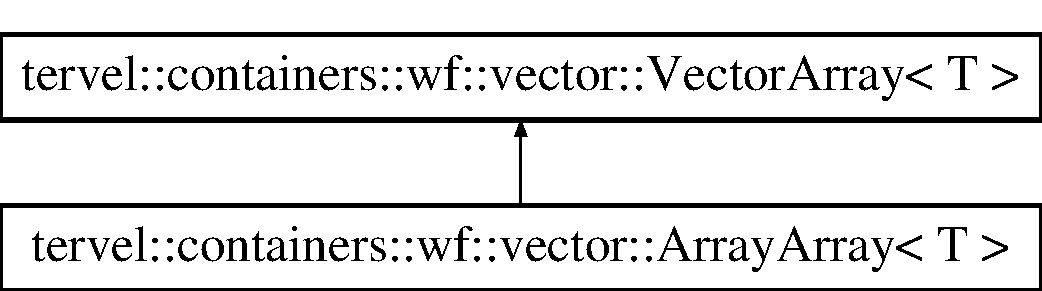
\includegraphics[height=2.000000cm]{classtervel_1_1containers_1_1wf_1_1vector_1_1_vector_array}
\end{center}
\end{figure}
\subsection*{Public Member Functions}
\begin{DoxyCompactItemize}
\item 
\hyperlink{classtervel_1_1containers_1_1wf_1_1vector_1_1_vector_array_aed082fd2b69025f00bedd363c65cf83c}{Vector\+Array} ()
\item 
\hyperlink{classtervel_1_1containers_1_1wf_1_1vector_1_1_vector_array_ac685bbc4b704949073f3ac73d8c6ade7}{Vector\+Array} (size\+\_\+t capacity)
\item 
virtual \hyperlink{classtervel_1_1containers_1_1wf_1_1vector_1_1_vector_array_aea78805a55da50a537dd0533df091db6}{$\sim$\+Vector\+Array} ()
\item 
virtual std\+::atomic$<$ T $>$ $\ast$ \hyperlink{classtervel_1_1containers_1_1wf_1_1vector_1_1_vector_array_a1ff5c1a5a86a822cfd50b48987d1857b}{get\+\_\+spot} (const size\+\_\+t raw\+\_\+pos, const bool no\+\_\+add=false)=0
\begin{DoxyCompactList}\small\item\em This function returns the address of the specified position. \end{DoxyCompactList}\item 
virtual bool \hyperlink{classtervel_1_1containers_1_1wf_1_1vector_1_1_vector_array_a46c74b691caae714a87bc93e793083f9}{is\+\_\+valid} (T value)
\item 
virtual bool \hyperlink{classtervel_1_1containers_1_1wf_1_1vector_1_1_vector_array_a03f1f7712b35cb9fc7d5f9bc4a89dd96}{is\+\_\+descriptor} (T \&expected, std\+::atomic$<$ T $>$ $\ast$spot)
\begin{DoxyCompactList}\small\item\em Overridden by Single\+Array model to detect resize. \end{DoxyCompactList}\end{DoxyCompactItemize}


\subsection{Constructor \& Destructor Documentation}
\hypertarget{classtervel_1_1containers_1_1wf_1_1vector_1_1_vector_array_aed082fd2b69025f00bedd363c65cf83c}{}\index{tervel\+::containers\+::wf\+::vector\+::\+Vector\+Array@{tervel\+::containers\+::wf\+::vector\+::\+Vector\+Array}!Vector\+Array@{Vector\+Array}}
\index{Vector\+Array@{Vector\+Array}!tervel\+::containers\+::wf\+::vector\+::\+Vector\+Array@{tervel\+::containers\+::wf\+::vector\+::\+Vector\+Array}}
\subsubsection[{Vector\+Array()}]{\setlength{\rightskip}{0pt plus 5cm}template$<$typename T $>$ {\bf tervel\+::containers\+::wf\+::vector\+::\+Vector\+Array}$<$ T $>$\+::{\bf Vector\+Array} (
\begin{DoxyParamCaption}
{}
\end{DoxyParamCaption}
)\hspace{0.3cm}{\ttfamily [inline]}, {\ttfamily [explicit]}}\label{classtervel_1_1containers_1_1wf_1_1vector_1_1_vector_array_aed082fd2b69025f00bedd363c65cf83c}
\hypertarget{classtervel_1_1containers_1_1wf_1_1vector_1_1_vector_array_ac685bbc4b704949073f3ac73d8c6ade7}{}\index{tervel\+::containers\+::wf\+::vector\+::\+Vector\+Array@{tervel\+::containers\+::wf\+::vector\+::\+Vector\+Array}!Vector\+Array@{Vector\+Array}}
\index{Vector\+Array@{Vector\+Array}!tervel\+::containers\+::wf\+::vector\+::\+Vector\+Array@{tervel\+::containers\+::wf\+::vector\+::\+Vector\+Array}}
\subsubsection[{Vector\+Array(size\+\_\+t capacity)}]{\setlength{\rightskip}{0pt plus 5cm}template$<$typename T $>$ {\bf tervel\+::containers\+::wf\+::vector\+::\+Vector\+Array}$<$ T $>$\+::{\bf Vector\+Array} (
\begin{DoxyParamCaption}
\item[{size\+\_\+t}]{capacity}
\end{DoxyParamCaption}
)\hspace{0.3cm}{\ttfamily [inline]}, {\ttfamily [explicit]}}\label{classtervel_1_1containers_1_1wf_1_1vector_1_1_vector_array_ac685bbc4b704949073f3ac73d8c6ade7}
\hypertarget{classtervel_1_1containers_1_1wf_1_1vector_1_1_vector_array_aea78805a55da50a537dd0533df091db6}{}\index{tervel\+::containers\+::wf\+::vector\+::\+Vector\+Array@{tervel\+::containers\+::wf\+::vector\+::\+Vector\+Array}!````~Vector\+Array@{$\sim$\+Vector\+Array}}
\index{````~Vector\+Array@{$\sim$\+Vector\+Array}!tervel\+::containers\+::wf\+::vector\+::\+Vector\+Array@{tervel\+::containers\+::wf\+::vector\+::\+Vector\+Array}}
\subsubsection[{$\sim$\+Vector\+Array()}]{\setlength{\rightskip}{0pt plus 5cm}template$<$typename T $>$ virtual {\bf tervel\+::containers\+::wf\+::vector\+::\+Vector\+Array}$<$ T $>$\+::$\sim${\bf Vector\+Array} (
\begin{DoxyParamCaption}
{}
\end{DoxyParamCaption}
)\hspace{0.3cm}{\ttfamily [inline]}, {\ttfamily [virtual]}}\label{classtervel_1_1containers_1_1wf_1_1vector_1_1_vector_array_aea78805a55da50a537dd0533df091db6}


\subsection{Member Function Documentation}
\hypertarget{classtervel_1_1containers_1_1wf_1_1vector_1_1_vector_array_a1ff5c1a5a86a822cfd50b48987d1857b}{}\index{tervel\+::containers\+::wf\+::vector\+::\+Vector\+Array@{tervel\+::containers\+::wf\+::vector\+::\+Vector\+Array}!get\+\_\+spot@{get\+\_\+spot}}
\index{get\+\_\+spot@{get\+\_\+spot}!tervel\+::containers\+::wf\+::vector\+::\+Vector\+Array@{tervel\+::containers\+::wf\+::vector\+::\+Vector\+Array}}
\subsubsection[{get\+\_\+spot(const size\+\_\+t raw\+\_\+pos, const bool no\+\_\+add=false)=0}]{\setlength{\rightskip}{0pt plus 5cm}template$<$typename T $>$ virtual std\+::atomic$<$T$>$$\ast$ {\bf tervel\+::containers\+::wf\+::vector\+::\+Vector\+Array}$<$ T $>$\+::get\+\_\+spot (
\begin{DoxyParamCaption}
\item[{const size\+\_\+t}]{raw\+\_\+pos, }
\item[{const bool}]{no\+\_\+add = {\ttfamily false}}
\end{DoxyParamCaption}
)\hspace{0.3cm}{\ttfamily [pure virtual]}}\label{classtervel_1_1containers_1_1wf_1_1vector_1_1_vector_array_a1ff5c1a5a86a822cfd50b48987d1857b}


This function returns the address of the specified position. 


\begin{DoxyParams}{Parameters}
{\em raw\+\_\+pos} & the position \\
\hline
{\em no\+\_\+add} & if true then it will not increase the vectors size \\
\hline
\end{DoxyParams}
\begin{DoxyReturn}{Returns}
the address of the specified position 
\end{DoxyReturn}


Implemented in \hyperlink{classtervel_1_1containers_1_1wf_1_1vector_1_1_array_array_afaa4f7502ab5ae8ccbe7bb05408f600a}{tervel\+::containers\+::wf\+::vector\+::\+Array\+Array$<$ T $>$}.

\hypertarget{classtervel_1_1containers_1_1wf_1_1vector_1_1_vector_array_a03f1f7712b35cb9fc7d5f9bc4a89dd96}{}\index{tervel\+::containers\+::wf\+::vector\+::\+Vector\+Array@{tervel\+::containers\+::wf\+::vector\+::\+Vector\+Array}!is\+\_\+descriptor@{is\+\_\+descriptor}}
\index{is\+\_\+descriptor@{is\+\_\+descriptor}!tervel\+::containers\+::wf\+::vector\+::\+Vector\+Array@{tervel\+::containers\+::wf\+::vector\+::\+Vector\+Array}}
\subsubsection[{is\+\_\+descriptor(\+T \&expected, std\+::atomic$<$ T $>$ $\ast$spot)}]{\setlength{\rightskip}{0pt plus 5cm}template$<$typename T $>$ virtual bool {\bf tervel\+::containers\+::wf\+::vector\+::\+Vector\+Array}$<$ T $>$\+::is\+\_\+descriptor (
\begin{DoxyParamCaption}
\item[{T \&}]{expected, }
\item[{std\+::atomic$<$ T $>$ $\ast$}]{spot}
\end{DoxyParamCaption}
)\hspace{0.3cm}{\ttfamily [inline]}, {\ttfamily [virtual]}}\label{classtervel_1_1containers_1_1wf_1_1vector_1_1_vector_array_a03f1f7712b35cb9fc7d5f9bc4a89dd96}


Overridden by Single\+Array model to detect resize. 


\begin{DoxyParams}{Parameters}
{\em expected} & \mbox{[}description\mbox{]} \\
\hline
{\em spot} & \mbox{[}description\mbox{]} \\
\hline
\end{DoxyParams}
\begin{DoxyReturn}{Returns}
\mbox{[}description\mbox{]} 
\end{DoxyReturn}
\hypertarget{classtervel_1_1containers_1_1wf_1_1vector_1_1_vector_array_a46c74b691caae714a87bc93e793083f9}{}\index{tervel\+::containers\+::wf\+::vector\+::\+Vector\+Array@{tervel\+::containers\+::wf\+::vector\+::\+Vector\+Array}!is\+\_\+valid@{is\+\_\+valid}}
\index{is\+\_\+valid@{is\+\_\+valid}!tervel\+::containers\+::wf\+::vector\+::\+Vector\+Array@{tervel\+::containers\+::wf\+::vector\+::\+Vector\+Array}}
\subsubsection[{is\+\_\+valid(\+T value)}]{\setlength{\rightskip}{0pt plus 5cm}template$<$typename T $>$ virtual bool {\bf tervel\+::containers\+::wf\+::vector\+::\+Vector\+Array}$<$ T $>$\+::is\+\_\+valid (
\begin{DoxyParamCaption}
\item[{T}]{value}
\end{DoxyParamCaption}
)\hspace{0.3cm}{\ttfamily [inline]}, {\ttfamily [virtual]}}\label{classtervel_1_1containers_1_1wf_1_1vector_1_1_vector_array_a46c74b691caae714a87bc93e793083f9}


The documentation for this class was generated from the following file\+:\begin{DoxyCompactItemize}
\item 
tervel/containers/wf/vector/\hyperlink{vector__array_8h}{vector\+\_\+array.\+h}\end{DoxyCompactItemize}

\hypertarget{class_test_class_1_1_wrapper_type}{}\section{Test\+Class$<$ Key, Value $>$\+:\+:Wrapper\+Type Class Reference}
\label{class_test_class_1_1_wrapper_type}\index{Test\+Class$<$ Key, Value $>$\+::\+Wrapper\+Type@{Test\+Class$<$ Key, Value $>$\+::\+Wrapper\+Type}}


{\ttfamily \#include $<$wf\+\_\+ringbuffer\+\_\+api.\+h$>$}

Inheritance diagram for Test\+Class$<$ Key, Value $>$\+:\+:Wrapper\+Type\+:\begin{figure}[H]
\begin{center}
\leavevmode
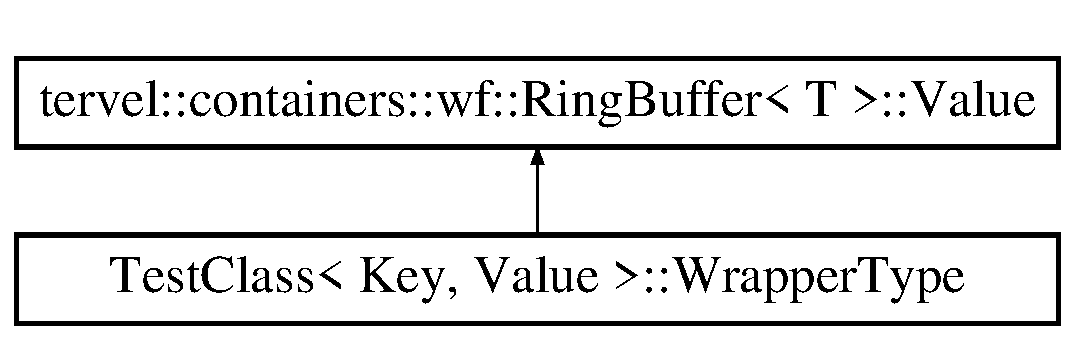
\includegraphics[height=2.000000cm]{class_test_class_1_1_wrapper_type}
\end{center}
\end{figure}
\subsection*{Public Member Functions}
\begin{DoxyCompactItemize}
\item 
\hyperlink{class_test_class_1_1_wrapper_type_a2b0268ce9a34cd9c0f2b8467183fb318}{Wrapper\+Type} (\hyperlink{hash__map_2test_object_8h_ad777bf08d8e2b01df17ba5e3c51ae11f}{Value} x)
\item 
\hyperlink{hash__map_2test_object_8h_ad777bf08d8e2b01df17ba5e3c51ae11f}{Value} \hyperlink{class_test_class_1_1_wrapper_type_a4fcbd1e5ed510805606d3598b00a96ec}{value} ()
\item 
std\+::string \hyperlink{class_test_class_1_1_wrapper_type_acd68ad5a338a5ad57708c9d912401a3f}{to\+String} ()
\end{DoxyCompactItemize}
\subsection*{Private Attributes}
\begin{DoxyCompactItemize}
\item 
const \hyperlink{hash__map_2test_object_8h_ad777bf08d8e2b01df17ba5e3c51ae11f}{Value} \hyperlink{class_test_class_1_1_wrapper_type_a54229b2608aca867a7c60ac474072fad}{x\+\_\+}
\end{DoxyCompactItemize}
\subsection*{Additional Inherited Members}


\subsection{Constructor \& Destructor Documentation}
\hypertarget{class_test_class_1_1_wrapper_type_a2b0268ce9a34cd9c0f2b8467183fb318}{}\index{Test\+Class\+::\+Wrapper\+Type@{Test\+Class\+::\+Wrapper\+Type}!Wrapper\+Type@{Wrapper\+Type}}
\index{Wrapper\+Type@{Wrapper\+Type}!Test\+Class\+::\+Wrapper\+Type@{Test\+Class\+::\+Wrapper\+Type}}
\subsubsection[{Wrapper\+Type(\+Value x)}]{\setlength{\rightskip}{0pt plus 5cm}template$<$class Key, class Value$>$ {\bf Test\+Class}$<$ Key, {\bf Value} $>$\+::Wrapper\+Type\+::\+Wrapper\+Type (
\begin{DoxyParamCaption}
\item[{{\bf Value}}]{x}
\end{DoxyParamCaption}
)\hspace{0.3cm}{\ttfamily [inline]}}\label{class_test_class_1_1_wrapper_type_a2b0268ce9a34cd9c0f2b8467183fb318}


\subsection{Member Function Documentation}
\hypertarget{class_test_class_1_1_wrapper_type_acd68ad5a338a5ad57708c9d912401a3f}{}\index{Test\+Class\+::\+Wrapper\+Type@{Test\+Class\+::\+Wrapper\+Type}!to\+String@{to\+String}}
\index{to\+String@{to\+String}!Test\+Class\+::\+Wrapper\+Type@{Test\+Class\+::\+Wrapper\+Type}}
\subsubsection[{to\+String()}]{\setlength{\rightskip}{0pt plus 5cm}template$<$class Key, class Value$>$ std\+::string {\bf Test\+Class}$<$ Key, {\bf Value} $>$\+::Wrapper\+Type\+::to\+String (
\begin{DoxyParamCaption}
{}
\end{DoxyParamCaption}
)\hspace{0.3cm}{\ttfamily [inline]}}\label{class_test_class_1_1_wrapper_type_acd68ad5a338a5ad57708c9d912401a3f}
\hypertarget{class_test_class_1_1_wrapper_type_a4fcbd1e5ed510805606d3598b00a96ec}{}\index{Test\+Class\+::\+Wrapper\+Type@{Test\+Class\+::\+Wrapper\+Type}!value@{value}}
\index{value@{value}!Test\+Class\+::\+Wrapper\+Type@{Test\+Class\+::\+Wrapper\+Type}}
\subsubsection[{value()}]{\setlength{\rightskip}{0pt plus 5cm}template$<$class Key, class Value$>$ {\bf Value} {\bf Test\+Class}$<$ Key, {\bf Value} $>$\+::Wrapper\+Type\+::value (
\begin{DoxyParamCaption}
{}
\end{DoxyParamCaption}
)\hspace{0.3cm}{\ttfamily [inline]}}\label{class_test_class_1_1_wrapper_type_a4fcbd1e5ed510805606d3598b00a96ec}


\subsection{Member Data Documentation}
\hypertarget{class_test_class_1_1_wrapper_type_a54229b2608aca867a7c60ac474072fad}{}\index{Test\+Class\+::\+Wrapper\+Type@{Test\+Class\+::\+Wrapper\+Type}!x\+\_\+@{x\+\_\+}}
\index{x\+\_\+@{x\+\_\+}!Test\+Class\+::\+Wrapper\+Type@{Test\+Class\+::\+Wrapper\+Type}}
\subsubsection[{x\+\_\+}]{\setlength{\rightskip}{0pt plus 5cm}template$<$class Key, class Value$>$ const {\bf Value} {\bf Test\+Class}$<$ Key, {\bf Value} $>$\+::Wrapper\+Type\+::x\+\_\+\hspace{0.3cm}{\ttfamily [private]}}\label{class_test_class_1_1_wrapper_type_a54229b2608aca867a7c60ac474072fad}


The documentation for this class was generated from the following file\+:\begin{DoxyCompactItemize}
\item 
tervel/tests/ring-\/buffer/api/\hyperlink{wf__ringbuffer__api_8h}{wf\+\_\+ringbuffer\+\_\+api.\+h}\end{DoxyCompactItemize}

\hypertarget{classtervel_1_1containers_1_1wf_1_1vector_1_1_write_helper}{}\section{tervel\+:\+:containers\+:\+:wf\+:\+:vector\+:\+:Write\+Helper$<$ T $>$ Class Template Reference}
\label{classtervel_1_1containers_1_1wf_1_1vector_1_1_write_helper}\index{tervel\+::containers\+::wf\+::vector\+::\+Write\+Helper$<$ T $>$@{tervel\+::containers\+::wf\+::vector\+::\+Write\+Helper$<$ T $>$}}


{\ttfamily \#include $<$write\+\_\+op.\+h$>$}

Inheritance diagram for tervel\+:\+:containers\+:\+:wf\+:\+:vector\+:\+:Write\+Helper$<$ T $>$\+:\begin{figure}[H]
\begin{center}
\leavevmode
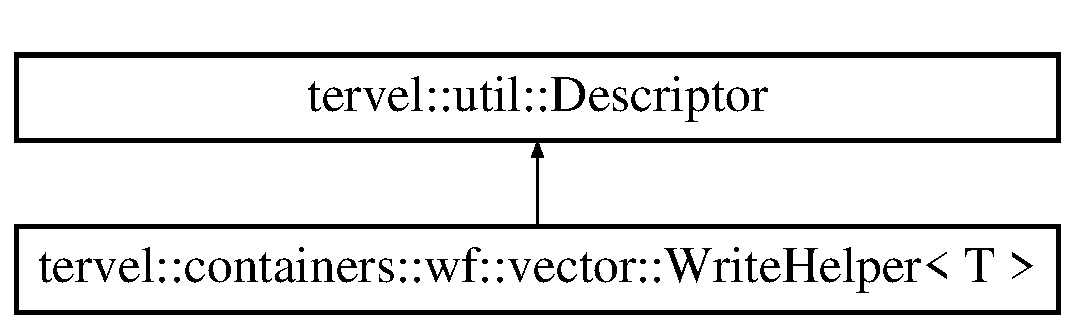
\includegraphics[height=2.000000cm]{classtervel_1_1containers_1_1wf_1_1vector_1_1_write_helper}
\end{center}
\end{figure}
\subsection*{Public Member Functions}
\begin{DoxyCompactItemize}
\item 
\hyperlink{classtervel_1_1containers_1_1wf_1_1vector_1_1_write_helper_aac69263d3e2c63fb2e5523042df4e627}{Write\+Helper} (\hyperlink{classtervel_1_1containers_1_1wf_1_1vector_1_1_write_op}{Write\+Op}$<$ T $>$ $\ast$op, T val)
\item 
T \hyperlink{classtervel_1_1containers_1_1wf_1_1vector_1_1_write_helper_a386891ae1b288469cc40e798289026fb}{value} ()
\item 
void $\ast$ \hyperlink{classtervel_1_1containers_1_1wf_1_1vector_1_1_write_helper_a379b580d78358bf8332119541d8e87c0}{complete} (void $\ast$\hyperlink{classtervel_1_1containers_1_1wf_1_1vector_1_1_write_helper_a386891ae1b288469cc40e798289026fb}{value}, std\+::atomic$<$ void $\ast$ $>$ $\ast$address)
\begin{DoxyCompactList}\small\item\em This method is implemented by each sub class and must guarantee that upon return that the descriptor no longer exists at the address it was placed. \end{DoxyCompactList}\item 
void $\ast$ \hyperlink{classtervel_1_1containers_1_1wf_1_1vector_1_1_write_helper_ae2c93c4fb9304dd82c25f5d8d9b23487}{get\+\_\+logical\+\_\+value} ()
\begin{DoxyCompactList}\small\item\em This method is implemented by each sub class. \end{DoxyCompactList}\item 
bool \hyperlink{classtervel_1_1containers_1_1wf_1_1vector_1_1_write_helper_a4c914b2218dfcfffaae66e85ff77e6df}{on\+\_\+watch} (std\+::atomic$<$ void $\ast$ $>$ $\ast$address, void $\ast$\hyperlink{classtervel_1_1containers_1_1wf_1_1vector_1_1_write_helper_a386891ae1b288469cc40e798289026fb}{value})
\begin{DoxyCompactList}\small\item\em This method is optional to implement for each sub class. \end{DoxyCompactList}\end{DoxyCompactItemize}
\subsection*{Private Attributes}
\begin{DoxyCompactItemize}
\item 
\hyperlink{classtervel_1_1containers_1_1wf_1_1vector_1_1_write_op}{Write\+Op}$<$ T $>$ $\ast$ \hyperlink{classtervel_1_1containers_1_1wf_1_1vector_1_1_write_helper_a4e3aac7ec85299353af06f639f1ce49e}{op\+\_\+}
\item 
const T \hyperlink{classtervel_1_1containers_1_1wf_1_1vector_1_1_write_helper_a5ccc8c44a16ff3d33c5472d0f149c771}{val\+\_\+}
\end{DoxyCompactItemize}
\subsection*{Friends}
\begin{DoxyCompactItemize}
\item 
class \hyperlink{classtervel_1_1containers_1_1wf_1_1vector_1_1_write_helper_ac7d62df5cf96a161e40f5741e00896cf}{Write\+Op$<$ T $>$}
\end{DoxyCompactItemize}


\subsection{Constructor \& Destructor Documentation}
\hypertarget{classtervel_1_1containers_1_1wf_1_1vector_1_1_write_helper_aac69263d3e2c63fb2e5523042df4e627}{}\index{tervel\+::containers\+::wf\+::vector\+::\+Write\+Helper@{tervel\+::containers\+::wf\+::vector\+::\+Write\+Helper}!Write\+Helper@{Write\+Helper}}
\index{Write\+Helper@{Write\+Helper}!tervel\+::containers\+::wf\+::vector\+::\+Write\+Helper@{tervel\+::containers\+::wf\+::vector\+::\+Write\+Helper}}
\subsubsection[{Write\+Helper(\+Write\+Op$<$ T $>$ $\ast$op, T val)}]{\setlength{\rightskip}{0pt plus 5cm}template$<$typename T$>$ {\bf tervel\+::containers\+::wf\+::vector\+::\+Write\+Helper}$<$ T $>$\+::{\bf Write\+Helper} (
\begin{DoxyParamCaption}
\item[{{\bf Write\+Op}$<$ T $>$ $\ast$}]{op, }
\item[{T}]{val}
\end{DoxyParamCaption}
)\hspace{0.3cm}{\ttfamily [inline]}, {\ttfamily [explicit]}}\label{classtervel_1_1containers_1_1wf_1_1vector_1_1_write_helper_aac69263d3e2c63fb2e5523042df4e627}


\subsection{Member Function Documentation}
\hypertarget{classtervel_1_1containers_1_1wf_1_1vector_1_1_write_helper_a379b580d78358bf8332119541d8e87c0}{}\index{tervel\+::containers\+::wf\+::vector\+::\+Write\+Helper@{tervel\+::containers\+::wf\+::vector\+::\+Write\+Helper}!complete@{complete}}
\index{complete@{complete}!tervel\+::containers\+::wf\+::vector\+::\+Write\+Helper@{tervel\+::containers\+::wf\+::vector\+::\+Write\+Helper}}
\subsubsection[{complete(void $\ast$value, std\+::atomic$<$ void $\ast$ $>$ $\ast$address)}]{\setlength{\rightskip}{0pt plus 5cm}template$<$typename T$>$ void$\ast$ {\bf tervel\+::containers\+::wf\+::vector\+::\+Write\+Helper}$<$ T $>$\+::complete (
\begin{DoxyParamCaption}
\item[{void $\ast$}]{current, }
\item[{std\+::atomic$<$ void $\ast$ $>$ $\ast$}]{address}
\end{DoxyParamCaption}
)\hspace{0.3cm}{\ttfamily [inline]}, {\ttfamily [virtual]}}\label{classtervel_1_1containers_1_1wf_1_1vector_1_1_write_helper_a379b580d78358bf8332119541d8e87c0}


This method is implemented by each sub class and must guarantee that upon return that the descriptor no longer exists at the address it was placed. 


\begin{DoxyParams}{Parameters}
{\em current} & the reference to this object as it is at the address, \\
\hline
{\em address} & the location this object was read from \\
\hline
\end{DoxyParams}


Implements \hyperlink{classtervel_1_1util_1_1_descriptor_a4303b2a08e3ab67de5533cfb20db87c9}{tervel\+::util\+::\+Descriptor}.

\hypertarget{classtervel_1_1containers_1_1wf_1_1vector_1_1_write_helper_ae2c93c4fb9304dd82c25f5d8d9b23487}{}\index{tervel\+::containers\+::wf\+::vector\+::\+Write\+Helper@{tervel\+::containers\+::wf\+::vector\+::\+Write\+Helper}!get\+\_\+logical\+\_\+value@{get\+\_\+logical\+\_\+value}}
\index{get\+\_\+logical\+\_\+value@{get\+\_\+logical\+\_\+value}!tervel\+::containers\+::wf\+::vector\+::\+Write\+Helper@{tervel\+::containers\+::wf\+::vector\+::\+Write\+Helper}}
\subsubsection[{get\+\_\+logical\+\_\+value()}]{\setlength{\rightskip}{0pt plus 5cm}template$<$typename T$>$ void$\ast$ {\bf tervel\+::containers\+::wf\+::vector\+::\+Write\+Helper}$<$ T $>$\+::get\+\_\+logical\+\_\+value (
\begin{DoxyParamCaption}
{}
\end{DoxyParamCaption}
)\hspace{0.3cm}{\ttfamily [inline]}, {\ttfamily [virtual]}}\label{classtervel_1_1containers_1_1wf_1_1vector_1_1_write_helper_ae2c93c4fb9304dd82c25f5d8d9b23487}


This method is implemented by each sub class. 

It returns the logical value of the past address. If the associated operation is still in progress then it will generally return the value that was replaced by this descriptor. Otherwise it will generally return the result of the operation for the specified address.

It can only be called from the static function which protects the object from being reused during the function. 

Implements \hyperlink{classtervel_1_1util_1_1_descriptor_a5b443eeb6acf1207f27a6d06c39d4ad4}{tervel\+::util\+::\+Descriptor}.

\hypertarget{classtervel_1_1containers_1_1wf_1_1vector_1_1_write_helper_a4c914b2218dfcfffaae66e85ff77e6df}{}\index{tervel\+::containers\+::wf\+::vector\+::\+Write\+Helper@{tervel\+::containers\+::wf\+::vector\+::\+Write\+Helper}!on\+\_\+watch@{on\+\_\+watch}}
\index{on\+\_\+watch@{on\+\_\+watch}!tervel\+::containers\+::wf\+::vector\+::\+Write\+Helper@{tervel\+::containers\+::wf\+::vector\+::\+Write\+Helper}}
\subsubsection[{on\+\_\+watch(std\+::atomic$<$ void $\ast$ $>$ $\ast$address, void $\ast$value)}]{\setlength{\rightskip}{0pt plus 5cm}template$<$typename T$>$ bool {\bf tervel\+::containers\+::wf\+::vector\+::\+Write\+Helper}$<$ T $>$\+::on\+\_\+watch (
\begin{DoxyParamCaption}
\item[{std\+::atomic$<$ void $\ast$ $>$ $\ast$}]{, }
\item[{void $\ast$}]{}
\end{DoxyParamCaption}
)\hspace{0.3cm}{\ttfamily [inline]}, {\ttfamily [virtual]}}\label{classtervel_1_1containers_1_1wf_1_1vector_1_1_write_helper_a4c914b2218dfcfffaae66e85ff77e6df}


This method is optional to implement for each sub class. 

In the event there is a complex dependency between descriptor objects, where watching one implies performing other actions, such as watching a parent object, a developer will implement this function to encapsulate that logic

This function is called by the static watch function It should not watch itself.


\begin{DoxyParams}{Parameters}
{\em address} & The location to check. \\
\hline
{\em expected} & The expected value for that location\\
\hline
\end{DoxyParams}
\begin{DoxyReturn}{Returns}
true if successful, false otherwise 
\end{DoxyReturn}


Reimplemented from \hyperlink{classtervel_1_1util_1_1_descriptor_ab643e09f20f35149dc820766b0f9ccdb}{tervel\+::util\+::\+Descriptor}.

\hypertarget{classtervel_1_1containers_1_1wf_1_1vector_1_1_write_helper_a386891ae1b288469cc40e798289026fb}{}\index{tervel\+::containers\+::wf\+::vector\+::\+Write\+Helper@{tervel\+::containers\+::wf\+::vector\+::\+Write\+Helper}!value@{value}}
\index{value@{value}!tervel\+::containers\+::wf\+::vector\+::\+Write\+Helper@{tervel\+::containers\+::wf\+::vector\+::\+Write\+Helper}}
\subsubsection[{value()}]{\setlength{\rightskip}{0pt plus 5cm}template$<$typename T$>$ T {\bf tervel\+::containers\+::wf\+::vector\+::\+Write\+Helper}$<$ T $>$\+::value (
\begin{DoxyParamCaption}
{}
\end{DoxyParamCaption}
)\hspace{0.3cm}{\ttfamily [inline]}}\label{classtervel_1_1containers_1_1wf_1_1vector_1_1_write_helper_a386891ae1b288469cc40e798289026fb}


\subsection{Friends And Related Function Documentation}
\hypertarget{classtervel_1_1containers_1_1wf_1_1vector_1_1_write_helper_ac7d62df5cf96a161e40f5741e00896cf}{}\index{tervel\+::containers\+::wf\+::vector\+::\+Write\+Helper@{tervel\+::containers\+::wf\+::vector\+::\+Write\+Helper}!Write\+Op$<$ T $>$@{Write\+Op$<$ T $>$}}
\index{Write\+Op$<$ T $>$@{Write\+Op$<$ T $>$}!tervel\+::containers\+::wf\+::vector\+::\+Write\+Helper@{tervel\+::containers\+::wf\+::vector\+::\+Write\+Helper}}
\subsubsection[{Write\+Op$<$ T $>$}]{\setlength{\rightskip}{0pt plus 5cm}template$<$typename T$>$ friend class {\bf Write\+Op}$<$ T $>$\hspace{0.3cm}{\ttfamily [friend]}}\label{classtervel_1_1containers_1_1wf_1_1vector_1_1_write_helper_ac7d62df5cf96a161e40f5741e00896cf}


\subsection{Member Data Documentation}
\hypertarget{classtervel_1_1containers_1_1wf_1_1vector_1_1_write_helper_a4e3aac7ec85299353af06f639f1ce49e}{}\index{tervel\+::containers\+::wf\+::vector\+::\+Write\+Helper@{tervel\+::containers\+::wf\+::vector\+::\+Write\+Helper}!op\+\_\+@{op\+\_\+}}
\index{op\+\_\+@{op\+\_\+}!tervel\+::containers\+::wf\+::vector\+::\+Write\+Helper@{tervel\+::containers\+::wf\+::vector\+::\+Write\+Helper}}
\subsubsection[{op\+\_\+}]{\setlength{\rightskip}{0pt plus 5cm}template$<$typename T$>$ {\bf Write\+Op}$<$T$>$$\ast$ {\bf tervel\+::containers\+::wf\+::vector\+::\+Write\+Helper}$<$ T $>$\+::op\+\_\+\hspace{0.3cm}{\ttfamily [private]}}\label{classtervel_1_1containers_1_1wf_1_1vector_1_1_write_helper_a4e3aac7ec85299353af06f639f1ce49e}
\hypertarget{classtervel_1_1containers_1_1wf_1_1vector_1_1_write_helper_a5ccc8c44a16ff3d33c5472d0f149c771}{}\index{tervel\+::containers\+::wf\+::vector\+::\+Write\+Helper@{tervel\+::containers\+::wf\+::vector\+::\+Write\+Helper}!val\+\_\+@{val\+\_\+}}
\index{val\+\_\+@{val\+\_\+}!tervel\+::containers\+::wf\+::vector\+::\+Write\+Helper@{tervel\+::containers\+::wf\+::vector\+::\+Write\+Helper}}
\subsubsection[{val\+\_\+}]{\setlength{\rightskip}{0pt plus 5cm}template$<$typename T$>$ const T {\bf tervel\+::containers\+::wf\+::vector\+::\+Write\+Helper}$<$ T $>$\+::val\+\_\+\hspace{0.3cm}{\ttfamily [private]}}\label{classtervel_1_1containers_1_1wf_1_1vector_1_1_write_helper_a5ccc8c44a16ff3d33c5472d0f149c771}


The documentation for this class was generated from the following file\+:\begin{DoxyCompactItemize}
\item 
tervel/containers/wf/vector/\hyperlink{write__op_8h}{write\+\_\+op.\+h}\end{DoxyCompactItemize}

\hypertarget{classtervel_1_1containers_1_1wf_1_1vector_1_1_write_op}{}\section{tervel\+:\+:containers\+:\+:wf\+:\+:vector\+:\+:Write\+Op$<$ T $>$ Class Template Reference}
\label{classtervel_1_1containers_1_1wf_1_1vector_1_1_write_op}\index{tervel\+::containers\+::wf\+::vector\+::\+Write\+Op$<$ T $>$@{tervel\+::containers\+::wf\+::vector\+::\+Write\+Op$<$ T $>$}}


{\ttfamily \#include $<$write\+\_\+op.\+h$>$}

Inheritance diagram for tervel\+:\+:containers\+:\+:wf\+:\+:vector\+:\+:Write\+Op$<$ T $>$\+:\begin{figure}[H]
\begin{center}
\leavevmode
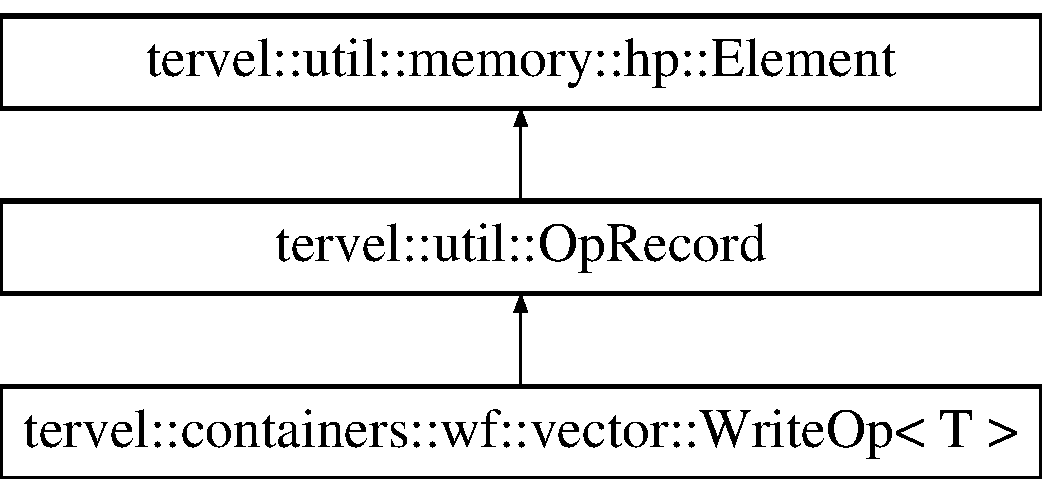
\includegraphics[height=3.000000cm]{classtervel_1_1containers_1_1wf_1_1vector_1_1_write_op}
\end{center}
\end{figure}
\subsection*{Public Member Functions}
\begin{DoxyCompactItemize}
\item 
\hyperlink{classtervel_1_1containers_1_1wf_1_1vector_1_1_write_op_a09e0c8cc62247a95e50e43a482df81fe}{Write\+Op} (Vector$<$ T $>$ $\ast$vec, size\+\_\+t idx, T expected, T val)
\item 
\hyperlink{classtervel_1_1containers_1_1wf_1_1vector_1_1_write_op_a80cc81812cda1b0b3d379e883106fb51}{$\sim$\+Write\+Op} ()
\item 
void \hyperlink{classtervel_1_1containers_1_1wf_1_1vector_1_1_write_op_a30f4a6d0e37b6e591fb986977304e08d}{help\+\_\+complete} ()
\begin{DoxyCompactList}\small\item\em Implementations of this function that upon its return the operation described in the Op\+Record has been completed. \end{DoxyCompactList}\item 
bool \hyperlink{classtervel_1_1containers_1_1wf_1_1vector_1_1_write_op_a972e53578716571f63bca13af4fe8f16}{result} (T \&expected)
\item 
bool \hyperlink{classtervel_1_1containers_1_1wf_1_1vector_1_1_write_op_ab9b31a254a96f4b7b04c3ae66bda8eca}{is\+\_\+watched} ()
\end{DoxyCompactItemize}
\subsection*{Private Attributes}
\begin{DoxyCompactItemize}
\item 
Vector$<$ T $>$ $\ast$ \hyperlink{classtervel_1_1containers_1_1wf_1_1vector_1_1_write_op_aad0429090bde2576091caa8ef1713cda}{vec\+\_\+}
\item 
size\+\_\+t \hyperlink{classtervel_1_1containers_1_1wf_1_1vector_1_1_write_op_adeee65a9fa4dbe774d09e29356884ea5}{idx\+\_\+}
\item 
T \hyperlink{classtervel_1_1containers_1_1wf_1_1vector_1_1_write_op_a50dce7c9fe835edf72033b665057bc05}{expected\+\_\+}
\item 
T \hyperlink{classtervel_1_1containers_1_1wf_1_1vector_1_1_write_op_af75188ef94bec379f9fafb55248491f2}{new\+\_\+val\+\_\+}
\item 
std\+::atomic$<$ \hyperlink{classtervel_1_1containers_1_1wf_1_1vector_1_1_write_helper}{Write\+Helper}$<$ T $>$ $\ast$ $>$ \hyperlink{classtervel_1_1containers_1_1wf_1_1vector_1_1_write_op_ab1239b5ef9dfcabbd9bb4626b036fb3b}{helper\+\_\+} \{nullptr\}
\end{DoxyCompactItemize}
\subsection*{Friends}
\begin{DoxyCompactItemize}
\item 
class \hyperlink{classtervel_1_1containers_1_1wf_1_1vector_1_1_write_op_a9f30cc5e47d15bd8dd0d486bb2dd026b}{Write\+Helper$<$ T $>$}
\end{DoxyCompactItemize}


\subsection{Constructor \& Destructor Documentation}
\hypertarget{classtervel_1_1containers_1_1wf_1_1vector_1_1_write_op_a09e0c8cc62247a95e50e43a482df81fe}{}\index{tervel\+::containers\+::wf\+::vector\+::\+Write\+Op@{tervel\+::containers\+::wf\+::vector\+::\+Write\+Op}!Write\+Op@{Write\+Op}}
\index{Write\+Op@{Write\+Op}!tervel\+::containers\+::wf\+::vector\+::\+Write\+Op@{tervel\+::containers\+::wf\+::vector\+::\+Write\+Op}}
\subsubsection[{Write\+Op(\+Vector$<$ T $>$ $\ast$vec, size\+\_\+t idx, T expected, T val)}]{\setlength{\rightskip}{0pt plus 5cm}template$<$typename T$>$ {\bf tervel\+::containers\+::wf\+::vector\+::\+Write\+Op}$<$ T $>$\+::{\bf Write\+Op} (
\begin{DoxyParamCaption}
\item[{Vector$<$ T $>$ $\ast$}]{vec, }
\item[{size\+\_\+t}]{idx, }
\item[{T}]{expected, }
\item[{T}]{val}
\end{DoxyParamCaption}
)\hspace{0.3cm}{\ttfamily [inline]}}\label{classtervel_1_1containers_1_1wf_1_1vector_1_1_write_op_a09e0c8cc62247a95e50e43a482df81fe}
\hypertarget{classtervel_1_1containers_1_1wf_1_1vector_1_1_write_op_a80cc81812cda1b0b3d379e883106fb51}{}\index{tervel\+::containers\+::wf\+::vector\+::\+Write\+Op@{tervel\+::containers\+::wf\+::vector\+::\+Write\+Op}!````~Write\+Op@{$\sim$\+Write\+Op}}
\index{````~Write\+Op@{$\sim$\+Write\+Op}!tervel\+::containers\+::wf\+::vector\+::\+Write\+Op@{tervel\+::containers\+::wf\+::vector\+::\+Write\+Op}}
\subsubsection[{$\sim$\+Write\+Op()}]{\setlength{\rightskip}{0pt plus 5cm}template$<$typename T$>$ {\bf tervel\+::containers\+::wf\+::vector\+::\+Write\+Op}$<$ T $>$\+::$\sim${\bf Write\+Op} (
\begin{DoxyParamCaption}
{}
\end{DoxyParamCaption}
)\hspace{0.3cm}{\ttfamily [inline]}}\label{classtervel_1_1containers_1_1wf_1_1vector_1_1_write_op_a80cc81812cda1b0b3d379e883106fb51}


\subsection{Member Function Documentation}
\hypertarget{classtervel_1_1containers_1_1wf_1_1vector_1_1_write_op_a30f4a6d0e37b6e591fb986977304e08d}{}\index{tervel\+::containers\+::wf\+::vector\+::\+Write\+Op@{tervel\+::containers\+::wf\+::vector\+::\+Write\+Op}!help\+\_\+complete@{help\+\_\+complete}}
\index{help\+\_\+complete@{help\+\_\+complete}!tervel\+::containers\+::wf\+::vector\+::\+Write\+Op@{tervel\+::containers\+::wf\+::vector\+::\+Write\+Op}}
\subsubsection[{help\+\_\+complete()}]{\setlength{\rightskip}{0pt plus 5cm}template$<$typename T$>$ void {\bf tervel\+::containers\+::wf\+::vector\+::\+Write\+Op}$<$ T $>$\+::help\+\_\+complete (
\begin{DoxyParamCaption}
{}
\end{DoxyParamCaption}
)\hspace{0.3cm}{\ttfamily [inline]}, {\ttfamily [virtual]}}\label{classtervel_1_1containers_1_1wf_1_1vector_1_1_write_op_a30f4a6d0e37b6e591fb986977304e08d}


Implementations of this function that upon its return the operation described in the Op\+Record has been completed. 

As such it must be thread-\/safe and the extending class must contain all the information necessary to complete the operation. 

Implements \hyperlink{classtervel_1_1util_1_1_op_record_aa75ab39688a8d4cceb6a1ef0409537c0}{tervel\+::util\+::\+Op\+Record}.

\hypertarget{classtervel_1_1containers_1_1wf_1_1vector_1_1_write_op_ab9b31a254a96f4b7b04c3ae66bda8eca}{}\index{tervel\+::containers\+::wf\+::vector\+::\+Write\+Op@{tervel\+::containers\+::wf\+::vector\+::\+Write\+Op}!is\+\_\+watched@{is\+\_\+watched}}
\index{is\+\_\+watched@{is\+\_\+watched}!tervel\+::containers\+::wf\+::vector\+::\+Write\+Op@{tervel\+::containers\+::wf\+::vector\+::\+Write\+Op}}
\subsubsection[{is\+\_\+watched()}]{\setlength{\rightskip}{0pt plus 5cm}template$<$typename T$>$ bool {\bf tervel\+::containers\+::wf\+::vector\+::\+Write\+Op}$<$ T $>$\+::is\+\_\+watched (
\begin{DoxyParamCaption}
{}
\end{DoxyParamCaption}
)\hspace{0.3cm}{\ttfamily [inline]}}\label{classtervel_1_1containers_1_1wf_1_1vector_1_1_write_op_ab9b31a254a96f4b7b04c3ae66bda8eca}
\hypertarget{classtervel_1_1containers_1_1wf_1_1vector_1_1_write_op_a972e53578716571f63bca13af4fe8f16}{}\index{tervel\+::containers\+::wf\+::vector\+::\+Write\+Op@{tervel\+::containers\+::wf\+::vector\+::\+Write\+Op}!result@{result}}
\index{result@{result}!tervel\+::containers\+::wf\+::vector\+::\+Write\+Op@{tervel\+::containers\+::wf\+::vector\+::\+Write\+Op}}
\subsubsection[{result(\+T \&expected)}]{\setlength{\rightskip}{0pt plus 5cm}template$<$typename T$>$ bool {\bf tervel\+::containers\+::wf\+::vector\+::\+Write\+Op}$<$ T $>$\+::result (
\begin{DoxyParamCaption}
\item[{T \&}]{expected}
\end{DoxyParamCaption}
)\hspace{0.3cm}{\ttfamily [inline]}}\label{classtervel_1_1containers_1_1wf_1_1vector_1_1_write_op_a972e53578716571f63bca13af4fe8f16}


\subsection{Friends And Related Function Documentation}
\hypertarget{classtervel_1_1containers_1_1wf_1_1vector_1_1_write_op_a9f30cc5e47d15bd8dd0d486bb2dd026b}{}\index{tervel\+::containers\+::wf\+::vector\+::\+Write\+Op@{tervel\+::containers\+::wf\+::vector\+::\+Write\+Op}!Write\+Helper$<$ T $>$@{Write\+Helper$<$ T $>$}}
\index{Write\+Helper$<$ T $>$@{Write\+Helper$<$ T $>$}!tervel\+::containers\+::wf\+::vector\+::\+Write\+Op@{tervel\+::containers\+::wf\+::vector\+::\+Write\+Op}}
\subsubsection[{Write\+Helper$<$ T $>$}]{\setlength{\rightskip}{0pt plus 5cm}template$<$typename T$>$ friend class {\bf Write\+Helper}$<$ T $>$\hspace{0.3cm}{\ttfamily [friend]}}\label{classtervel_1_1containers_1_1wf_1_1vector_1_1_write_op_a9f30cc5e47d15bd8dd0d486bb2dd026b}


\subsection{Member Data Documentation}
\hypertarget{classtervel_1_1containers_1_1wf_1_1vector_1_1_write_op_a50dce7c9fe835edf72033b665057bc05}{}\index{tervel\+::containers\+::wf\+::vector\+::\+Write\+Op@{tervel\+::containers\+::wf\+::vector\+::\+Write\+Op}!expected\+\_\+@{expected\+\_\+}}
\index{expected\+\_\+@{expected\+\_\+}!tervel\+::containers\+::wf\+::vector\+::\+Write\+Op@{tervel\+::containers\+::wf\+::vector\+::\+Write\+Op}}
\subsubsection[{expected\+\_\+}]{\setlength{\rightskip}{0pt plus 5cm}template$<$typename T$>$ T {\bf tervel\+::containers\+::wf\+::vector\+::\+Write\+Op}$<$ T $>$\+::expected\+\_\+\hspace{0.3cm}{\ttfamily [private]}}\label{classtervel_1_1containers_1_1wf_1_1vector_1_1_write_op_a50dce7c9fe835edf72033b665057bc05}
\hypertarget{classtervel_1_1containers_1_1wf_1_1vector_1_1_write_op_ab1239b5ef9dfcabbd9bb4626b036fb3b}{}\index{tervel\+::containers\+::wf\+::vector\+::\+Write\+Op@{tervel\+::containers\+::wf\+::vector\+::\+Write\+Op}!helper\+\_\+@{helper\+\_\+}}
\index{helper\+\_\+@{helper\+\_\+}!tervel\+::containers\+::wf\+::vector\+::\+Write\+Op@{tervel\+::containers\+::wf\+::vector\+::\+Write\+Op}}
\subsubsection[{helper\+\_\+}]{\setlength{\rightskip}{0pt plus 5cm}template$<$typename T$>$ std\+::atomic$<${\bf Write\+Helper}$<$T$>$ $\ast$$>$ {\bf tervel\+::containers\+::wf\+::vector\+::\+Write\+Op}$<$ T $>$\+::helper\+\_\+ \{nullptr\}\hspace{0.3cm}{\ttfamily [private]}}\label{classtervel_1_1containers_1_1wf_1_1vector_1_1_write_op_ab1239b5ef9dfcabbd9bb4626b036fb3b}
\hypertarget{classtervel_1_1containers_1_1wf_1_1vector_1_1_write_op_adeee65a9fa4dbe774d09e29356884ea5}{}\index{tervel\+::containers\+::wf\+::vector\+::\+Write\+Op@{tervel\+::containers\+::wf\+::vector\+::\+Write\+Op}!idx\+\_\+@{idx\+\_\+}}
\index{idx\+\_\+@{idx\+\_\+}!tervel\+::containers\+::wf\+::vector\+::\+Write\+Op@{tervel\+::containers\+::wf\+::vector\+::\+Write\+Op}}
\subsubsection[{idx\+\_\+}]{\setlength{\rightskip}{0pt plus 5cm}template$<$typename T$>$ size\+\_\+t {\bf tervel\+::containers\+::wf\+::vector\+::\+Write\+Op}$<$ T $>$\+::idx\+\_\+\hspace{0.3cm}{\ttfamily [private]}}\label{classtervel_1_1containers_1_1wf_1_1vector_1_1_write_op_adeee65a9fa4dbe774d09e29356884ea5}
\hypertarget{classtervel_1_1containers_1_1wf_1_1vector_1_1_write_op_af75188ef94bec379f9fafb55248491f2}{}\index{tervel\+::containers\+::wf\+::vector\+::\+Write\+Op@{tervel\+::containers\+::wf\+::vector\+::\+Write\+Op}!new\+\_\+val\+\_\+@{new\+\_\+val\+\_\+}}
\index{new\+\_\+val\+\_\+@{new\+\_\+val\+\_\+}!tervel\+::containers\+::wf\+::vector\+::\+Write\+Op@{tervel\+::containers\+::wf\+::vector\+::\+Write\+Op}}
\subsubsection[{new\+\_\+val\+\_\+}]{\setlength{\rightskip}{0pt plus 5cm}template$<$typename T$>$ T {\bf tervel\+::containers\+::wf\+::vector\+::\+Write\+Op}$<$ T $>$\+::new\+\_\+val\+\_\+\hspace{0.3cm}{\ttfamily [private]}}\label{classtervel_1_1containers_1_1wf_1_1vector_1_1_write_op_af75188ef94bec379f9fafb55248491f2}
\hypertarget{classtervel_1_1containers_1_1wf_1_1vector_1_1_write_op_aad0429090bde2576091caa8ef1713cda}{}\index{tervel\+::containers\+::wf\+::vector\+::\+Write\+Op@{tervel\+::containers\+::wf\+::vector\+::\+Write\+Op}!vec\+\_\+@{vec\+\_\+}}
\index{vec\+\_\+@{vec\+\_\+}!tervel\+::containers\+::wf\+::vector\+::\+Write\+Op@{tervel\+::containers\+::wf\+::vector\+::\+Write\+Op}}
\subsubsection[{vec\+\_\+}]{\setlength{\rightskip}{0pt plus 5cm}template$<$typename T$>$ Vector$<$T$>$$\ast$ {\bf tervel\+::containers\+::wf\+::vector\+::\+Write\+Op}$<$ T $>$\+::vec\+\_\+\hspace{0.3cm}{\ttfamily [private]}}\label{classtervel_1_1containers_1_1wf_1_1vector_1_1_write_op_aad0429090bde2576091caa8ef1713cda}


The documentation for this class was generated from the following file\+:\begin{DoxyCompactItemize}
\item 
tervel/containers/wf/vector/\hyperlink{write__op_8h}{write\+\_\+op.\+h}\end{DoxyCompactItemize}

\chapter{File Documentation}
\hypertarget{mcas_8h}{}\section{tervel/algorithms/wf/mcas/mcas.h File Reference}
\label{mcas_8h}\index{tervel/algorithms/wf/mcas/mcas.\+h@{tervel/algorithms/wf/mcas/mcas.\+h}}
{\ttfamily \#include $<$tervel/util/info.\+h$>$}\\*
{\ttfamily \#include $<$tervel/util/util.\+h$>$}\\*
{\ttfamily \#include $<$tervel/util/progress\+\_\+assurance.\+h$>$}\\*
{\ttfamily \#include $<$tervel/util/memory/rc/descriptor\+\_\+util.\+h$>$}\\*
{\ttfamily \#include $<$tervel/algorithms/wf/mcas/mcas\+\_\+helper.\+h$>$}\\*
{\ttfamily \#include $<$tervel/algorithms/wf/mcas/mcas\+\_\+casrow.\+h$>$}\\*
{\ttfamily \#include $<$tervel/algorithms/wf/mcas/mcas\+\_\+imp.\+h$>$}\\*
\subsection*{Classes}
\begin{DoxyCompactItemize}
\item 
class \hyperlink{classtervel_1_1algorithms_1_1wf_1_1mcas_1_1_multi_word_compare_and_swap}{tervel\+::algorithms\+::wf\+::mcas\+::\+Multi\+Word\+Compare\+And\+Swap$<$ T $>$}
\begin{DoxyCompactList}\small\item\em \hyperlink{classtervel_1_1algorithms_1_1wf_1_1mcas_1_1_multi_word_compare_and_swap}{Multi\+Word\+Compare\+And\+Swap} class is used to perform a Multi-\/\+Word Compare-\/and-\/\+Swap (\hyperlink{classtervel_1_1algorithms_1_1wf_1_1mcas_1_1_m_c_a_s}{M\+C\+A\+S}) To execute an \hyperlink{classtervel_1_1algorithms_1_1wf_1_1mcas_1_1_m_c_a_s}{M\+C\+A\+S}, call add\+C\+A\+S\+Triple for each address you want to update, then call \hyperlink{classtervel_1_1algorithms_1_1wf_1_1mcas_1_1_multi_word_compare_and_swap_a3cf56f32c7579f734b1e0ecbd8d9c7f3}{execute()};. \end{DoxyCompactList}\end{DoxyCompactItemize}
\subsection*{Namespaces}
\begin{DoxyCompactItemize}
\item 
 \hyperlink{namespacetervel}{tervel}
\begin{DoxyCompactList}\small\item\em T\+O\+D\+O(steven)\+: \end{DoxyCompactList}\item 
 \hyperlink{namespacetervel_1_1algorithms}{tervel\+::algorithms}
\item 
 \hyperlink{namespacetervel_1_1algorithms_1_1wf}{tervel\+::algorithms\+::wf}
\item 
 \hyperlink{namespacetervel_1_1algorithms_1_1wf_1_1mcas}{tervel\+::algorithms\+::wf\+::mcas}
\end{DoxyCompactItemize}
\subsection*{Functions}
\begin{DoxyCompactItemize}
\item 
{\footnotesize template$<$class T $>$ }\\T \hyperlink{namespacetervel_1_1algorithms_1_1wf_1_1mcas_a5abaf235e4abd3bd1f9f372c5d914d08}{tervel\+::algorithms\+::wf\+::mcas\+::read} (std\+::atomic$<$ T $>$ $\ast$address)
\begin{DoxyCompactList}\small\item\em This function determines the logical value of the address. \end{DoxyCompactList}\end{DoxyCompactItemize}

\hypertarget{mcas__casrow_8h}{}\section{tervel/algorithms/wf/mcas/mcas\+\_\+casrow.h File Reference}
\label{mcas__casrow_8h}\index{tervel/algorithms/wf/mcas/mcas\+\_\+casrow.\+h@{tervel/algorithms/wf/mcas/mcas\+\_\+casrow.\+h}}
{\ttfamily \#include $<$tervel/util/info.\+h$>$}\\*
{\ttfamily \#include $<$tervel/algorithms/wf/mcas/mcas\+\_\+helper.\+h$>$}\\*
\subsection*{Classes}
\begin{DoxyCompactItemize}
\item 
class \hyperlink{classtervel_1_1algorithms_1_1wf_1_1mcas_1_1_helper}{tervel\+::algorithms\+::wf\+::mcas\+::\+Helper$<$ T $>$}
\begin{DoxyCompactList}\small\item\em This class is the \hyperlink{classtervel_1_1algorithms_1_1wf_1_1mcas_1_1_m_c_a_s}{M\+C\+A\+S} operation\textquotesingle{}s helper. \end{DoxyCompactList}\item 
class \hyperlink{classtervel_1_1algorithms_1_1wf_1_1mcas_1_1_cas_row}{tervel\+::algorithms\+::wf\+::mcas\+::\+Cas\+Row$<$ T $>$}
\begin{DoxyCompactList}\small\item\em This class is used to represent a one of the M C\+A\+S operations performed by an \hyperlink{classtervel_1_1algorithms_1_1wf_1_1mcas_1_1_m_c_a_s}{M\+C\+A\+S} operation. \end{DoxyCompactList}\end{DoxyCompactItemize}
\subsection*{Namespaces}
\begin{DoxyCompactItemize}
\item 
 \hyperlink{namespacetervel}{tervel}
\begin{DoxyCompactList}\small\item\em T\+O\+D\+O(steven)\+: \end{DoxyCompactList}\item 
 \hyperlink{namespacetervel_1_1algorithms}{tervel\+::algorithms}
\item 
 \hyperlink{namespacetervel_1_1algorithms_1_1wf}{tervel\+::algorithms\+::wf}
\item 
 \hyperlink{namespacetervel_1_1algorithms_1_1wf_1_1mcas}{tervel\+::algorithms\+::wf\+::mcas}
\end{DoxyCompactItemize}

\hypertarget{mcas__helper_8h}{}\section{tervel/algorithms/wf/mcas/mcas\+\_\+helper.h File Reference}
\label{mcas__helper_8h}\index{tervel/algorithms/wf/mcas/mcas\+\_\+helper.\+h@{tervel/algorithms/wf/mcas/mcas\+\_\+helper.\+h}}
{\ttfamily \#include $<$tervel/util/info.\+h$>$}\\*
{\ttfamily \#include $<$tervel/util/descriptor.\+h$>$}\\*
{\ttfamily \#include $<$tervel/util/memory/hp/hazard\+\_\+pointer.\+h$>$}\\*
{\ttfamily \#include $<$tervel/util/memory/rc/descriptor\+\_\+util.\+h$>$}\\*
{\ttfamily \#include $<$tervel/algorithms/wf/mcas/mcas.\+h$>$}\\*
{\ttfamily \#include $<$tervel/algorithms/wf/mcas/mcas\+\_\+casrow.\+h$>$}\\*
\subsection*{Classes}
\begin{DoxyCompactItemize}
\item 
class \hyperlink{classtervel_1_1algorithms_1_1wf_1_1mcas_1_1_m_c_a_s}{tervel\+::algorithms\+::wf\+::mcas\+::\+M\+C\+A\+S$<$ T $>$}
\item 
class \hyperlink{classtervel_1_1algorithms_1_1wf_1_1mcas_1_1_cas_row}{tervel\+::algorithms\+::wf\+::mcas\+::\+Cas\+Row$<$ T $>$}
\begin{DoxyCompactList}\small\item\em This class is used to represent a one of the M C\+A\+S operations performed by an \hyperlink{classtervel_1_1algorithms_1_1wf_1_1mcas_1_1_m_c_a_s}{M\+C\+A\+S} operation. \end{DoxyCompactList}\item 
class \hyperlink{classtervel_1_1algorithms_1_1wf_1_1mcas_1_1_helper}{tervel\+::algorithms\+::wf\+::mcas\+::\+Helper$<$ T $>$}
\begin{DoxyCompactList}\small\item\em This class is the \hyperlink{classtervel_1_1algorithms_1_1wf_1_1mcas_1_1_m_c_a_s}{M\+C\+A\+S} operation\textquotesingle{}s helper. \end{DoxyCompactList}\end{DoxyCompactItemize}
\subsection*{Namespaces}
\begin{DoxyCompactItemize}
\item 
 \hyperlink{namespacetervel}{tervel}
\begin{DoxyCompactList}\small\item\em T\+O\+D\+O(steven)\+: \end{DoxyCompactList}\item 
 \hyperlink{namespacetervel_1_1algorithms}{tervel\+::algorithms}
\item 
 \hyperlink{namespacetervel_1_1algorithms_1_1wf}{tervel\+::algorithms\+::wf}
\item 
 \hyperlink{namespacetervel_1_1algorithms_1_1wf_1_1mcas}{tervel\+::algorithms\+::wf\+::mcas}
\end{DoxyCompactItemize}

\hypertarget{mcas__imp_8h}{}\section{tervel/algorithms/wf/mcas/mcas\+\_\+imp.h File Reference}
\label{mcas__imp_8h}\index{tervel/algorithms/wf/mcas/mcas\+\_\+imp.\+h@{tervel/algorithms/wf/mcas/mcas\+\_\+imp.\+h}}
\subsection*{Namespaces}
\begin{DoxyCompactItemize}
\item 
 \hyperlink{namespacetervel}{tervel}
\begin{DoxyCompactList}\small\item\em T\+O\+D\+O(steven)\+: \end{DoxyCompactList}\item 
 \hyperlink{namespacetervel_1_1algorithms}{tervel\+::algorithms}
\item 
 \hyperlink{namespacetervel_1_1algorithms_1_1wf}{tervel\+::algorithms\+::wf}
\item 
 \hyperlink{namespacetervel_1_1algorithms_1_1wf_1_1mcas}{tervel\+::algorithms\+::wf\+::mcas}
\end{DoxyCompactItemize}

\hypertarget{mcas__buffer_8h}{}\section{tervel/containers/lf/mcas-\/buffer/mcas\+\_\+buffer.h File Reference}
\label{mcas__buffer_8h}\index{tervel/containers/lf/mcas-\/buffer/mcas\+\_\+buffer.\+h@{tervel/containers/lf/mcas-\/buffer/mcas\+\_\+buffer.\+h}}
{\ttfamily \#include $<$atomic$>$}\\*
{\ttfamily \#include $<$cstdint$>$}\\*
{\ttfamily \#include $<$algorithm$>$}\\*
{\ttfamily \#include $<$tervel/util/info.\+h$>$}\\*
{\ttfamily \#include $<$tervel/util/memory/rc/descriptor\+\_\+util.\+h$>$}\\*
{\ttfamily \#include $<$tervel/util/descriptor.\+h$>$}\\*
{\ttfamily \#include $<$tervel/algorithms/wf/mcas/mcas.\+h$>$}\\*
\subsection*{Classes}
\begin{DoxyCompactItemize}
\item 
class \hyperlink{classtervel_1_1containers_1_1lf_1_1mcas__buffer_1_1_node}{tervel\+::containers\+::lf\+::mcas\+\_\+buffer\+::\+Node$<$ T $>$}
\item 
class \hyperlink{classtervel_1_1containers_1_1lf_1_1mcas__buffer_1_1_ring_buffer}{tervel\+::containers\+::lf\+::mcas\+\_\+buffer\+::\+Ring\+Buffer$<$ T $>$}
\end{DoxyCompactItemize}
\subsection*{Namespaces}
\begin{DoxyCompactItemize}
\item 
 \hyperlink{namespacetervel}{tervel}
\begin{DoxyCompactList}\small\item\em T\+O\+D\+O(steven)\+: \end{DoxyCompactList}\item 
 \hyperlink{namespacetervel_1_1containers}{tervel\+::containers}
\item 
 \hyperlink{namespacetervel_1_1containers_1_1lf}{tervel\+::containers\+::lf}
\item 
 \hyperlink{namespacetervel_1_1containers_1_1lf_1_1mcas__buffer}{tervel\+::containers\+::lf\+::mcas\+\_\+buffer}
\end{DoxyCompactItemize}

\hypertarget{wf__hash__map_8h}{}\section{tervel/containers/wf/hash-\/map/wf\+\_\+hash\+\_\+map.h File Reference}
\label{wf__hash__map_8h}\index{tervel/containers/wf/hash-\/map/wf\+\_\+hash\+\_\+map.\+h@{tervel/containers/wf/hash-\/map/wf\+\_\+hash\+\_\+map.\+h}}
{\ttfamily \#include $<$tervel/util/info.\+h$>$}\\*
{\ttfamily \#include $<$tervel/util/memory/hp/hp\+\_\+element.\+h$>$}\\*
{\ttfamily \#include $<$tervel/util/memory/hp/hazard\+\_\+pointer.\+h$>$}\\*
{\ttfamily \#include $<$tervel/util/progress\+\_\+assurance.\+h$>$}\\*
\subsection*{Classes}
\begin{DoxyCompactItemize}
\item 
struct \hyperlink{structtervel_1_1containers_1_1wf_1_1default__functor}{tervel\+::containers\+::wf\+::default\+\_\+functor$<$ Key, Value $>$}
\begin{DoxyCompactList}\small\item\em A default Functor implementation. \end{DoxyCompactList}\item 
class \hyperlink{classtervel_1_1containers_1_1wf_1_1_hash_map}{tervel\+::containers\+::wf\+::\+Hash\+Map$<$ Key, Value, Functor $>$}
\begin{DoxyCompactList}\small\item\em A wait-\/free hash map implementation. \end{DoxyCompactList}\item 
class \hyperlink{classtervel_1_1containers_1_1wf_1_1_hash_map_1_1_value_accessor}{tervel\+::containers\+::wf\+::\+Hash\+Map$<$ Key, Value, Functor $>$\+::\+Value\+Accessor}
\begin{DoxyCompactList}\small\item\em This class is used to safe guard access to values. \end{DoxyCompactList}\item 
class \hyperlink{classtervel_1_1containers_1_1wf_1_1_hash_map_1_1_node}{tervel\+::containers\+::wf\+::\+Hash\+Map$<$ Key, Value, Functor $>$\+::\+Node}
\begin{DoxyCompactList}\small\item\em This class is used to differentiate between data\+\_\+nodes and array\+\_\+nodes/. \end{DoxyCompactList}\item 
class \hyperlink{classtervel_1_1containers_1_1wf_1_1_hash_map_1_1_array_node}{tervel\+::containers\+::wf\+::\+Hash\+Map$<$ Key, Value, Functor $>$\+::\+Array\+Node}
\begin{DoxyCompactList}\small\item\em This class is used to hold the secondary array structure. \end{DoxyCompactList}\item 
class \hyperlink{classtervel_1_1containers_1_1wf_1_1_hash_map_1_1_data_node}{tervel\+::containers\+::wf\+::\+Hash\+Map$<$ Key, Value, Functor $>$\+::\+Data\+Node}
\begin{DoxyCompactList}\small\item\em This class is used to hold a key and value pair. \end{DoxyCompactList}\item 
class \hyperlink{classtervel_1_1containers_1_1wf_1_1_hash_map_1_1_force_expand_op}{tervel\+::containers\+::wf\+::\+Hash\+Map$<$ Key, Value, Functor $>$\+::\+Force\+Expand\+Op}
\begin{DoxyCompactList}\small\item\em T\+O\+D\+O(steven)\+: add description T\+O\+D\+O(steven)\+: move into a file. \end{DoxyCompactList}\end{DoxyCompactItemize}
\subsection*{Namespaces}
\begin{DoxyCompactItemize}
\item 
 \hyperlink{namespacetervel}{tervel}
\begin{DoxyCompactList}\small\item\em T\+O\+D\+O(steven)\+: \end{DoxyCompactList}\item 
 \hyperlink{namespacetervel_1_1containers}{tervel\+::containers}
\item 
 \hyperlink{namespacetervel_1_1containers_1_1wf}{tervel\+::containers\+::wf}
\end{DoxyCompactItemize}

\hypertarget{wf__hash__map__no__delete_8h}{}\section{tervel/containers/wf/hash-\/map/wf\+\_\+hash\+\_\+map\+\_\+no\+\_\+delete.h File Reference}
\label{wf__hash__map__no__delete_8h}\index{tervel/containers/wf/hash-\/map/wf\+\_\+hash\+\_\+map\+\_\+no\+\_\+delete.\+h@{tervel/containers/wf/hash-\/map/wf\+\_\+hash\+\_\+map\+\_\+no\+\_\+delete.\+h}}
{\ttfamily \#include $<$stdlib.\+h$>$}\\*
{\ttfamily \#include $<$atomic$>$}\\*
{\ttfamily \#include $<$cmath$>$}\\*
\subsection*{Classes}
\begin{DoxyCompactItemize}
\item 
struct \hyperlink{structtervel_1_1containers_1_1wf_1_1default__functor}{tervel\+::containers\+::wf\+::default\+\_\+functor$<$ Key, Value $>$}
\begin{DoxyCompactList}\small\item\em A default Functor implementation. \end{DoxyCompactList}\item 
class \hyperlink{classtervel_1_1containers_1_1wf_1_1_hash_map_no_delete}{tervel\+::containers\+::wf\+::\+Hash\+Map\+No\+Delete$<$ Key, Value, Functor $>$}
\begin{DoxyCompactList}\small\item\em A wait-\/free hash map implementation. \end{DoxyCompactList}\item 
class \hyperlink{classtervel_1_1containers_1_1wf_1_1_hash_map_no_delete_1_1_value_accessor}{tervel\+::containers\+::wf\+::\+Hash\+Map\+No\+Delete$<$ Key, Value, Functor $>$\+::\+Value\+Accessor}
\begin{DoxyCompactList}\small\item\em This class is used to safe guard access to values. \end{DoxyCompactList}\item 
class \hyperlink{classtervel_1_1containers_1_1wf_1_1_hash_map_no_delete_1_1_node}{tervel\+::containers\+::wf\+::\+Hash\+Map\+No\+Delete$<$ Key, Value, Functor $>$\+::\+Node}
\begin{DoxyCompactList}\small\item\em This class is used to differentiate between data\+\_\+nodes and array\+\_\+nodes/. \end{DoxyCompactList}\item 
class \hyperlink{classtervel_1_1containers_1_1wf_1_1_hash_map_no_delete_1_1_array_node}{tervel\+::containers\+::wf\+::\+Hash\+Map\+No\+Delete$<$ Key, Value, Functor $>$\+::\+Array\+Node}
\begin{DoxyCompactList}\small\item\em This class is used to hold the secondary array structure. \end{DoxyCompactList}\item 
class \hyperlink{classtervel_1_1containers_1_1wf_1_1_hash_map_no_delete_1_1_data_node}{tervel\+::containers\+::wf\+::\+Hash\+Map\+No\+Delete$<$ Key, Value, Functor $>$\+::\+Data\+Node}
\begin{DoxyCompactList}\small\item\em This class is used to hold a key and value pair. \end{DoxyCompactList}\end{DoxyCompactItemize}
\subsection*{Namespaces}
\begin{DoxyCompactItemize}
\item 
 \hyperlink{namespacetervel}{tervel}
\begin{DoxyCompactList}\small\item\em T\+O\+D\+O(steven)\+: \end{DoxyCompactList}\item 
 \hyperlink{namespacetervel_1_1util}{tervel\+::util}
\item 
 \hyperlink{namespacetervel_1_1containers}{tervel\+::containers}
\item 
 \hyperlink{namespacetervel_1_1containers_1_1wf}{tervel\+::containers\+::wf}
\end{DoxyCompactItemize}
\subsection*{Functions}
\begin{DoxyCompactItemize}
\item 
int \hyperlink{namespacetervel_1_1util_a8fa82e619afb1d31d761c703a9aad97b}{tervel\+::util\+::round\+\_\+to\+\_\+next\+\_\+power\+\_\+of\+\_\+two} (uint64\+\_\+t value)
\begin{DoxyCompactList}\small\item\em Returns the next power of two. \end{DoxyCompactList}\end{DoxyCompactItemize}

\hypertarget{dequeue__op_8h}{}\section{tervel/containers/wf/ring-\/buffer/dequeue\+\_\+op.h File Reference}
\label{dequeue__op_8h}\index{tervel/containers/wf/ring-\/buffer/dequeue\+\_\+op.\+h@{tervel/containers/wf/ring-\/buffer/dequeue\+\_\+op.\+h}}
{\ttfamily \#include $<$tervel/containers/wf/ring-\/buffer/ring\+\_\+buffer\+\_\+op.\+h$>$}\\*
\subsection*{Classes}
\begin{DoxyCompactItemize}
\item 
class \hyperlink{classtervel_1_1containers_1_1wf_1_1_ring_buffer_1_1_dequeue_op}{tervel\+::containers\+::wf\+::\+Ring\+Buffer$<$ T $>$\+::\+Dequeue\+Op$<$ T $>$}
\end{DoxyCompactItemize}
\subsection*{Namespaces}
\begin{DoxyCompactItemize}
\item 
 \hyperlink{namespacetervel}{tervel}
\begin{DoxyCompactList}\small\item\em T\+O\+D\+O(steven)\+: \end{DoxyCompactList}\item 
 \hyperlink{namespacetervel_1_1containers}{tervel\+::containers}
\item 
 \hyperlink{namespacetervel_1_1containers_1_1wf}{tervel\+::containers\+::wf}
\end{DoxyCompactItemize}

\hypertarget{dequeue__op__imp_8h}{}\section{tervel/containers/wf/ring-\/buffer/dequeue\+\_\+op\+\_\+imp.h File Reference}
\label{dequeue__op__imp_8h}\index{tervel/containers/wf/ring-\/buffer/dequeue\+\_\+op\+\_\+imp.\+h@{tervel/containers/wf/ring-\/buffer/dequeue\+\_\+op\+\_\+imp.\+h}}
{\ttfamily \#include $<$tervel/containers/wf/ring-\/buffer/dequeue\+\_\+op.\+h$>$}\\*
\subsection*{Namespaces}
\begin{DoxyCompactItemize}
\item 
 \hyperlink{namespacetervel}{tervel}
\begin{DoxyCompactList}\small\item\em T\+O\+D\+O(steven)\+: \end{DoxyCompactList}\item 
 \hyperlink{namespacetervel_1_1containers}{tervel\+::containers}
\item 
 \hyperlink{namespacetervel_1_1containers_1_1wf}{tervel\+::containers\+::wf}
\end{DoxyCompactItemize}

\hypertarget{enqueue__op_8h}{}\section{tervel/containers/wf/ring-\/buffer/enqueue\+\_\+op.h File Reference}
\label{enqueue__op_8h}\index{tervel/containers/wf/ring-\/buffer/enqueue\+\_\+op.\+h@{tervel/containers/wf/ring-\/buffer/enqueue\+\_\+op.\+h}}
{\ttfamily \#include $<$tervel/containers/wf/ring-\/buffer/ring\+\_\+buffer\+\_\+op.\+h$>$}\\*
\subsection*{Classes}
\begin{DoxyCompactItemize}
\item 
class \hyperlink{classtervel_1_1containers_1_1wf_1_1_ring_buffer_1_1_enqueue_op}{tervel\+::containers\+::wf\+::\+Ring\+Buffer$<$ T $>$\+::\+Enqueue\+Op$<$ T $>$}
\end{DoxyCompactItemize}
\subsection*{Namespaces}
\begin{DoxyCompactItemize}
\item 
 \hyperlink{namespacetervel}{tervel}
\begin{DoxyCompactList}\small\item\em T\+O\+D\+O(steven)\+: \end{DoxyCompactList}\item 
 \hyperlink{namespacetervel_1_1containers}{tervel\+::containers}
\item 
 \hyperlink{namespacetervel_1_1containers_1_1wf}{tervel\+::containers\+::wf}
\end{DoxyCompactItemize}

\hypertarget{enqueue__op__imp_8h}{}\section{tervel/containers/wf/ring-\/buffer/enqueue\+\_\+op\+\_\+imp.h File Reference}
\label{enqueue__op__imp_8h}\index{tervel/containers/wf/ring-\/buffer/enqueue\+\_\+op\+\_\+imp.\+h@{tervel/containers/wf/ring-\/buffer/enqueue\+\_\+op\+\_\+imp.\+h}}
{\ttfamily \#include $<$tervel/containers/wf/ring-\/buffer/enqueue\+\_\+op.\+h$>$}\\*
\subsection*{Namespaces}
\begin{DoxyCompactItemize}
\item 
 \hyperlink{namespacetervel}{tervel}
\begin{DoxyCompactList}\small\item\em T\+O\+D\+O(steven)\+: \end{DoxyCompactList}\item 
 \hyperlink{namespacetervel_1_1containers}{tervel\+::containers}
\item 
 \hyperlink{namespacetervel_1_1containers_1_1wf}{tervel\+::containers\+::wf}
\end{DoxyCompactItemize}

\hypertarget{helper_8h}{}\section{tervel/containers/wf/ring-\/buffer/helper.h File Reference}
\label{helper_8h}\index{tervel/containers/wf/ring-\/buffer/helper.\+h@{tervel/containers/wf/ring-\/buffer/helper.\+h}}
{\ttfamily \#include $<$tervel/util/memory/hp/hp\+\_\+element.\+h$>$}\\*
{\ttfamily \#include $<$tervel/util/memory/hp/hazard\+\_\+pointer.\+h$>$}\\*
\subsection*{Classes}
\begin{DoxyCompactItemize}
\item 
class \hyperlink{classtervel_1_1containers_1_1wf_1_1_ring_buffer_1_1_helper}{tervel\+::containers\+::wf\+::\+Ring\+Buffer$<$ T $>$\+::\+Helper$<$ T $>$}
\end{DoxyCompactItemize}
\subsection*{Namespaces}
\begin{DoxyCompactItemize}
\item 
 \hyperlink{namespacetervel}{tervel}
\begin{DoxyCompactList}\small\item\em T\+O\+D\+O(steven)\+: \end{DoxyCompactList}\item 
 \hyperlink{namespacetervel_1_1containers}{tervel\+::containers}
\item 
 \hyperlink{namespacetervel_1_1containers_1_1wf}{tervel\+::containers\+::wf}
\end{DoxyCompactItemize}

\hypertarget{helper__imp_8h}{}\section{tervel/containers/wf/ring-\/buffer/helper\+\_\+imp.h File Reference}
\label{helper__imp_8h}\index{tervel/containers/wf/ring-\/buffer/helper\+\_\+imp.\+h@{tervel/containers/wf/ring-\/buffer/helper\+\_\+imp.\+h}}
{\ttfamily \#include $<$tervel/util/memory/hp/hp\+\_\+element.\+h$>$}\\*
{\ttfamily \#include $<$tervel/util/memory/hp/hazard\+\_\+pointer.\+h$>$}\\*
{\ttfamily \#include $<$tervel/containers/wf/ring-\/buffer/helper.\+h$>$}\\*
\subsection*{Namespaces}
\begin{DoxyCompactItemize}
\item 
 \hyperlink{namespacetervel}{tervel}
\begin{DoxyCompactList}\small\item\em T\+O\+D\+O(steven)\+: \end{DoxyCompactList}\item 
 \hyperlink{namespacetervel_1_1containers}{tervel\+::containers}
\item 
 \hyperlink{namespacetervel_1_1containers_1_1wf}{tervel\+::containers\+::wf}
\end{DoxyCompactItemize}

\hypertarget{ring__buffer_8h}{}\section{tervel/containers/wf/ring-\/buffer/ring\+\_\+buffer.h File Reference}
\label{ring__buffer_8h}\index{tervel/containers/wf/ring-\/buffer/ring\+\_\+buffer.\+h@{tervel/containers/wf/ring-\/buffer/ring\+\_\+buffer.\+h}}
{\ttfamily \#include $<$atomic$>$}\\*
{\ttfamily \#include $<$assert.\+h$>$}\\*
{\ttfamily \#include $<$cstddef$>$}\\*
{\ttfamily \#include $<$memory$>$}\\*
{\ttfamily \#include $<$thread$>$}\\*
{\ttfamily \#include $<$string$>$}\\*
{\ttfamily \#include $<$tervel/util/info.\+h$>$}\\*
{\ttfamily \#include $<$tervel/util/util.\+h$>$}\\*
{\ttfamily \#include $<$tervel/util/progress\+\_\+assurance.\+h$>$}\\*
{\ttfamily \#include $<$tervel/util/memory/hp/hazard\+\_\+pointer.\+h$>$}\\*
{\ttfamily \#include $<$tervel/containers/wf/ring-\/buffer/ring\+\_\+buffer\+\_\+op.\+h$>$}\\*
{\ttfamily \#include $<$tervel/containers/wf/ring-\/buffer/helper.\+h$>$}\\*
{\ttfamily \#include $<$tervel/containers/wf/ring-\/buffer/enqueue\+\_\+op.\+h$>$}\\*
{\ttfamily \#include $<$tervel/containers/wf/ring-\/buffer/dequeue\+\_\+op.\+h$>$}\\*
{\ttfamily \#include $<$tervel/containers/wf/ring-\/buffer/helper\+\_\+imp.\+h$>$}\\*
{\ttfamily \#include $<$tervel/containers/wf/ring-\/buffer/enqueue\+\_\+op\+\_\+imp.\+h$>$}\\*
{\ttfamily \#include $<$tervel/containers/wf/ring-\/buffer/dequeue\+\_\+op\+\_\+imp.\+h$>$}\\*
{\ttfamily \#include $<$tervel/containers/wf/ring-\/buffer/ring\+\_\+buffer\+\_\+imp.\+h$>$}\\*
\subsection*{Classes}
\begin{DoxyCompactItemize}
\item 
class \hyperlink{classtervel_1_1containers_1_1wf_1_1_ring_buffer}{tervel\+::containers\+::wf\+::\+Ring\+Buffer$<$ T $>$}
\begin{DoxyCompactList}\small\item\em This is a non-\/blocking F\+I\+F\+O ring buffer design that was made wait-\/free by applying a progress assurance framework to it. \end{DoxyCompactList}\item 
class \hyperlink{classtervel_1_1containers_1_1wf_1_1_ring_buffer_1_1_value}{tervel\+::containers\+::wf\+::\+Ring\+Buffer$<$ T $>$\+::\+Value}
\begin{DoxyCompactList}\small\item\em \hyperlink{classtervel_1_1containers_1_1wf_1_1_ring_buffer}{Ring\+Buffer} value class, values stored in the class must extend it. \end{DoxyCompactList}\end{DoxyCompactItemize}
\subsection*{Namespaces}
\begin{DoxyCompactItemize}
\item 
 \hyperlink{namespacetervel}{tervel}
\begin{DoxyCompactList}\small\item\em T\+O\+D\+O(steven)\+: \end{DoxyCompactList}\item 
 \hyperlink{namespacetervel_1_1containers}{tervel\+::containers}
\item 
 \hyperlink{namespacetervel_1_1containers_1_1wf}{tervel\+::containers\+::wf}
\end{DoxyCompactItemize}

\hypertarget{ring__buffer__imp_8h}{}\section{tervel/containers/wf/ring-\/buffer/ring\+\_\+buffer\+\_\+imp.h File Reference}
\label{ring__buffer__imp_8h}\index{tervel/containers/wf/ring-\/buffer/ring\+\_\+buffer\+\_\+imp.\+h@{tervel/containers/wf/ring-\/buffer/ring\+\_\+buffer\+\_\+imp.\+h}}
\subsection*{Namespaces}
\begin{DoxyCompactItemize}
\item 
 \hyperlink{namespacetervel}{tervel}
\begin{DoxyCompactList}\small\item\em T\+O\+D\+O(steven)\+: \end{DoxyCompactList}\item 
 \hyperlink{namespacetervel_1_1containers}{tervel\+::containers}
\item 
 \hyperlink{namespacetervel_1_1containers_1_1wf}{tervel\+::containers\+::wf}
\end{DoxyCompactItemize}

\hypertarget{ring__buffer__op_8h}{}\section{tervel/containers/wf/ring-\/buffer/ring\+\_\+buffer\+\_\+op.h File Reference}
\label{ring__buffer__op_8h}\index{tervel/containers/wf/ring-\/buffer/ring\+\_\+buffer\+\_\+op.\+h@{tervel/containers/wf/ring-\/buffer/ring\+\_\+buffer\+\_\+op.\+h}}
{\ttfamily \#include $<$atomic$>$}\\*
{\ttfamily \#include $<$assert.\+h$>$}\\*
{\ttfamily \#include $<$cstddef$>$}\\*
{\ttfamily \#include $<$memory$>$}\\*
{\ttfamily \#include $<$thread$>$}\\*
{\ttfamily \#include $<$string$>$}\\*
{\ttfamily \#include $<$tervel/util/progress\+\_\+assurance.\+h$>$}\\*
{\ttfamily \#include $<$tervel/util/memory/hp/hp\+\_\+element.\+h$>$}\\*
{\ttfamily \#include $<$tervel/util/memory/hp/hazard\+\_\+pointer.\+h$>$}\\*
\subsection*{Classes}
\begin{DoxyCompactItemize}
\item 
class \hyperlink{classtervel_1_1containers_1_1wf_1_1_ring_buffer_1_1_buffer_op}{tervel\+::containers\+::wf\+::\+Ring\+Buffer$<$ T $>$\+::\+Buffer\+Op}
\end{DoxyCompactItemize}
\subsection*{Namespaces}
\begin{DoxyCompactItemize}
\item 
 \hyperlink{namespacetervel}{tervel}
\begin{DoxyCompactList}\small\item\em T\+O\+D\+O(steven)\+: \end{DoxyCompactList}\item 
 \hyperlink{namespacetervel_1_1containers}{tervel\+::containers}
\item 
 \hyperlink{namespacetervel_1_1containers_1_1wf}{tervel\+::containers\+::wf}
\end{DoxyCompactItemize}

\hypertarget{array__array_8h}{}\section{tervel/containers/wf/vector/array\+\_\+array.h File Reference}
\label{array__array_8h}\index{tervel/containers/wf/vector/array\+\_\+array.\+h@{tervel/containers/wf/vector/array\+\_\+array.\+h}}
{\ttfamily \#include $<$tervel/util/util.\+h$>$}\\*
{\ttfamily \#include $<$tervel/containers/wf/vector/vector\+\_\+array.\+h$>$}\\*
\subsection*{Classes}
\begin{DoxyCompactItemize}
\item 
class \hyperlink{classtervel_1_1containers_1_1wf_1_1vector_1_1_array_array}{tervel\+::containers\+::wf\+::vector\+::\+Array\+Array$<$ T $>$}
\end{DoxyCompactItemize}
\subsection*{Namespaces}
\begin{DoxyCompactItemize}
\item 
 \hyperlink{namespacetervel}{tervel}
\begin{DoxyCompactList}\small\item\em T\+O\+D\+O(steven)\+: \end{DoxyCompactList}\item 
 \hyperlink{namespacetervel_1_1containers}{tervel\+::containers}
\item 
 \hyperlink{namespacetervel_1_1containers_1_1wf}{tervel\+::containers\+::wf}
\item 
 \hyperlink{namespacetervel_1_1containers_1_1wf_1_1vector}{tervel\+::containers\+::wf\+::vector}
\end{DoxyCompactItemize}

\hypertarget{earaseat__op_8h}{}\section{tervel/containers/wf/vector/old/earaseat\+\_\+op.h File Reference}
\label{earaseat__op_8h}\index{tervel/containers/wf/vector/old/earaseat\+\_\+op.\+h@{tervel/containers/wf/vector/old/earaseat\+\_\+op.\+h}}
\subsection*{Classes}
\begin{DoxyCompactItemize}
\item 
class \hyperlink{class_erase_at}{Erase\+At$<$ T $>$}
\end{DoxyCompactItemize}

\hypertarget{insertat__op_8h}{}\section{tervel/containers/wf/vector/old/insertat\+\_\+op.h File Reference}
\label{insertat__op_8h}\index{tervel/containers/wf/vector/old/insertat\+\_\+op.\+h@{tervel/containers/wf/vector/old/insertat\+\_\+op.\+h}}
\subsection*{Classes}
\begin{DoxyCompactItemize}
\item 
class \hyperlink{class_insert_at}{Insert\+At}
\end{DoxyCompactItemize}

\hypertarget{pop__helper_8h}{}\section{tervel/containers/wf/vector/old/pop\+\_\+helper.h File Reference}
\label{pop__helper_8h}\index{tervel/containers/wf/vector/old/pop\+\_\+helper.\+h@{tervel/containers/wf/vector/old/pop\+\_\+helper.\+h}}
\subsection*{Classes}
\begin{DoxyCompactItemize}
\item 
class \hyperlink{class_pop_helper}{Pop\+Helper}
\item 
class \hyperlink{class_pop_sub_helper}{Pop\+Sub\+Helper}
\end{DoxyCompactItemize}

\hypertarget{pop__op_8h}{}\section{tervel/containers/wf/vector/old/pop\+\_\+op.h File Reference}
\label{pop__op_8h}\index{tervel/containers/wf/vector/old/pop\+\_\+op.\+h@{tervel/containers/wf/vector/old/pop\+\_\+op.\+h}}
\subsection*{Classes}
\begin{DoxyCompactItemize}
\item 
class \hyperlink{class_pop_op}{Pop\+Op}
\end{DoxyCompactItemize}

\hypertarget{push__helper_8h}{}\section{tervel/containers/wf/vector/old/push\+\_\+helper.h File Reference}
\label{push__helper_8h}\index{tervel/containers/wf/vector/old/push\+\_\+helper.\+h@{tervel/containers/wf/vector/old/push\+\_\+helper.\+h}}
\subsection*{Classes}
\begin{DoxyCompactItemize}
\item 
class \hyperlink{class_push_helper}{Push\+Helper}
\end{DoxyCompactItemize}

\hypertarget{push__op_8h}{}\section{tervel/containers/wf/vector/old/push\+\_\+op.h File Reference}
\label{push__op_8h}\index{tervel/containers/wf/vector/old/push\+\_\+op.\+h@{tervel/containers/wf/vector/old/push\+\_\+op.\+h}}
\subsection*{Classes}
\begin{DoxyCompactItemize}
\item 
class \hyperlink{class_push_op}{Push\+Op$<$ T $>$}
\end{DoxyCompactItemize}

\hypertarget{shift__helper_8h}{}\section{tervel/containers/wf/vector/old/shift\+\_\+helper.h File Reference}
\label{shift__helper_8h}\index{tervel/containers/wf/vector/old/shift\+\_\+helper.\+h@{tervel/containers/wf/vector/old/shift\+\_\+helper.\+h}}
{\ttfamily \#include \char`\"{}tervel/util/info.\+h\char`\"{}}\\*
{\ttfamily \#include \char`\"{}tervel/util/descriptor.\+h\char`\"{}}\\*
{\ttfamily \#include \char`\"{}tervel/util/memory/hp/hazard\+\_\+pointer.\+h\char`\"{}}\\*
{\ttfamily \#include \char`\"{}tervel/util/memory/rc/descriptor\+\_\+util.\+h\char`\"{}}\\*
\subsection*{Classes}
\begin{DoxyCompactItemize}
\item 
class \hyperlink{class_shift_helper}{Shift\+Helper$<$ Shift\+Op, T $>$}
\end{DoxyCompactItemize}
\subsection*{Functions}
\begin{DoxyCompactItemize}
\item 
{\footnotesize template$<$class Shift\+Type $>$ }\\bool \hyperlink{shift__helper_8h_a9ef2395bcf0df177f82c7138ce279352}{complete\+Shift} (Shift\+Type $\ast$op, W\+F\+Vector $\ast$vec, int pos)
\end{DoxyCompactItemize}


\subsection{Function Documentation}
\hypertarget{shift__helper_8h_a9ef2395bcf0df177f82c7138ce279352}{}\index{shift\+\_\+helper.\+h@{shift\+\_\+helper.\+h}!complete\+Shift@{complete\+Shift}}
\index{complete\+Shift@{complete\+Shift}!shift\+\_\+helper.\+h@{shift\+\_\+helper.\+h}}
\subsubsection[{complete\+Shift(\+Shift\+Type $\ast$op, W\+F\+Vector $\ast$vec, int pos)}]{\setlength{\rightskip}{0pt plus 5cm}template$<$class Shift\+Type $>$ bool complete\+Shift (
\begin{DoxyParamCaption}
\item[{Shift\+Type $\ast$}]{op, }
\item[{W\+F\+Vector $\ast$}]{vec, }
\item[{int}]{pos}
\end{DoxyParamCaption}
)}\label{shift__helper_8h_a9ef2395bcf0df177f82c7138ce279352}

\hypertarget{popback__op_8h}{}\section{tervel/containers/wf/vector/popback\+\_\+op.h File Reference}
\label{popback__op_8h}\index{tervel/containers/wf/vector/popback\+\_\+op.\+h@{tervel/containers/wf/vector/popback\+\_\+op.\+h}}
{\ttfamily \#include $<$tervel/util/info.\+h$>$}\\*
{\ttfamily \#include $<$tervel/util/descriptor.\+h$>$}\\*
{\ttfamily \#include $<$tervel/util/progress\+\_\+assurance.\+h$>$}\\*
{\ttfamily \#include $<$tervel/util/memory/hp/hazard\+\_\+pointer.\+h$>$}\\*
{\ttfamily \#include $<$tervel/util/memory/rc/descriptor\+\_\+util.\+h$>$}\\*
{\ttfamily \#include $<$tervel/containers/wf/vector/vector.\+hpp$>$}\\*
\subsection*{Classes}
\begin{DoxyCompactItemize}
\item 
class \hyperlink{classtervel_1_1containers_1_1wf_1_1vector_1_1_pop_op_helper}{tervel\+::containers\+::wf\+::vector\+::\+Pop\+Op\+Helper$<$ T $>$}
\item 
class \hyperlink{classtervel_1_1containers_1_1wf_1_1vector_1_1_pop_op_sub_helper}{tervel\+::containers\+::wf\+::vector\+::\+Pop\+Op\+Sub\+Helper$<$ T $>$}
\item 
class \hyperlink{classtervel_1_1containers_1_1wf_1_1vector_1_1_pop_op}{tervel\+::containers\+::wf\+::vector\+::\+Pop\+Op$<$ T $>$}
\item 
class \hyperlink{classtervel_1_1containers_1_1wf_1_1vector_1_1_pop_op_helper}{tervel\+::containers\+::wf\+::vector\+::\+Pop\+Op\+Helper$<$ T $>$}
\item 
class \hyperlink{classtervel_1_1containers_1_1wf_1_1vector_1_1_pop_op_sub_helper}{tervel\+::containers\+::wf\+::vector\+::\+Pop\+Op\+Sub\+Helper$<$ T $>$}
\end{DoxyCompactItemize}
\subsection*{Namespaces}
\begin{DoxyCompactItemize}
\item 
 \hyperlink{namespacetervel}{tervel}
\begin{DoxyCompactList}\small\item\em T\+O\+D\+O(steven)\+: \end{DoxyCompactList}\item 
 \hyperlink{namespacetervel_1_1containers}{tervel\+::containers}
\item 
 \hyperlink{namespacetervel_1_1containers_1_1wf}{tervel\+::containers\+::wf}
\item 
 \hyperlink{namespacetervel_1_1containers_1_1wf_1_1vector}{tervel\+::containers\+::wf\+::vector}
\end{DoxyCompactItemize}

\hypertarget{popbackwra__op_8h}{}\section{tervel/containers/wf/vector/popbackwra\+\_\+op.h File Reference}
\label{popbackwra__op_8h}\index{tervel/containers/wf/vector/popbackwra\+\_\+op.\+h@{tervel/containers/wf/vector/popbackwra\+\_\+op.\+h}}
{\ttfamily \#include $<$tervel/util/info.\+h$>$}\\*
{\ttfamily \#include $<$tervel/util/descriptor.\+h$>$}\\*
{\ttfamily \#include $<$tervel/util/progress\+\_\+assurance.\+h$>$}\\*
{\ttfamily \#include $<$tervel/util/memory/hp/hazard\+\_\+pointer.\+h$>$}\\*
{\ttfamily \#include $<$tervel/util/memory/rc/descriptor\+\_\+util.\+h$>$}\\*
{\ttfamily \#include $<$tervel/containers/wf/vector/vector.\+hpp$>$}\\*
\subsection*{Classes}
\begin{DoxyCompactItemize}
\item 
class \hyperlink{classtervel_1_1containers_1_1wf_1_1vector_1_1_pop_w_r_a_op_helper}{tervel\+::containers\+::wf\+::vector\+::\+Pop\+W\+R\+A\+Op\+Helper$<$ T $>$}
\item 
class \hyperlink{classtervel_1_1containers_1_1wf_1_1vector_1_1_pop_w_r_a_op}{tervel\+::containers\+::wf\+::vector\+::\+Pop\+W\+R\+A\+Op$<$ T $>$}
\item 
class \hyperlink{classtervel_1_1containers_1_1wf_1_1vector_1_1_pop_w_r_a_op_helper}{tervel\+::containers\+::wf\+::vector\+::\+Pop\+W\+R\+A\+Op\+Helper$<$ T $>$}
\end{DoxyCompactItemize}
\subsection*{Namespaces}
\begin{DoxyCompactItemize}
\item 
 \hyperlink{namespacetervel}{tervel}
\begin{DoxyCompactList}\small\item\em T\+O\+D\+O(steven)\+: \end{DoxyCompactList}\item 
 \hyperlink{namespacetervel_1_1containers}{tervel\+::containers}
\item 
 \hyperlink{namespacetervel_1_1containers_1_1wf}{tervel\+::containers\+::wf}
\item 
 \hyperlink{namespacetervel_1_1containers_1_1wf_1_1vector}{tervel\+::containers\+::wf\+::vector}
\end{DoxyCompactItemize}

\hypertarget{pushback__op_8h}{}\section{tervel/containers/wf/vector/pushback\+\_\+op.h File Reference}
\label{pushback__op_8h}\index{tervel/containers/wf/vector/pushback\+\_\+op.\+h@{tervel/containers/wf/vector/pushback\+\_\+op.\+h}}
{\ttfamily \#include $<$tervel/util/info.\+h$>$}\\*
{\ttfamily \#include $<$tervel/util/descriptor.\+h$>$}\\*
{\ttfamily \#include $<$tervel/util/progress\+\_\+assurance.\+h$>$}\\*
{\ttfamily \#include $<$tervel/util/memory/hp/hazard\+\_\+pointer.\+h$>$}\\*
{\ttfamily \#include $<$tervel/util/memory/rc/descriptor\+\_\+util.\+h$>$}\\*
{\ttfamily \#include $<$tervel/containers/wf/vector/vector.\+hpp$>$}\\*
\subsection*{Classes}
\begin{DoxyCompactItemize}
\item 
class \hyperlink{classtervel_1_1containers_1_1wf_1_1vector_1_1_push_op_helper}{tervel\+::containers\+::wf\+::vector\+::\+Push\+Op\+Helper$<$ T $>$}
\item 
class \hyperlink{classtervel_1_1containers_1_1wf_1_1vector_1_1_push_descr}{tervel\+::containers\+::wf\+::vector\+::\+Push\+Descr$<$ T $>$}
\item 
class \hyperlink{classtervel_1_1containers_1_1wf_1_1vector_1_1_push_op}{tervel\+::containers\+::wf\+::vector\+::\+Push\+Op$<$ T $>$}
\item 
class \hyperlink{classtervel_1_1containers_1_1wf_1_1vector_1_1_push_descr}{tervel\+::containers\+::wf\+::vector\+::\+Push\+Descr$<$ T $>$}
\item 
class \hyperlink{classtervel_1_1containers_1_1wf_1_1vector_1_1_push_op_helper}{tervel\+::containers\+::wf\+::vector\+::\+Push\+Op\+Helper$<$ T $>$}
\end{DoxyCompactItemize}
\subsection*{Namespaces}
\begin{DoxyCompactItemize}
\item 
 \hyperlink{namespacetervel}{tervel}
\begin{DoxyCompactList}\small\item\em T\+O\+D\+O(steven)\+: \end{DoxyCompactList}\item 
 \hyperlink{namespacetervel_1_1containers}{tervel\+::containers}
\item 
 \hyperlink{namespacetervel_1_1containers_1_1wf}{tervel\+::containers\+::wf}
\item 
 \hyperlink{namespacetervel_1_1containers_1_1wf_1_1vector}{tervel\+::containers\+::wf\+::vector}
\end{DoxyCompactItemize}

\hypertarget{pushbackwra__op_8h}{}\section{tervel/containers/wf/vector/pushbackwra\+\_\+op.h File Reference}
\label{pushbackwra__op_8h}\index{tervel/containers/wf/vector/pushbackwra\+\_\+op.\+h@{tervel/containers/wf/vector/pushbackwra\+\_\+op.\+h}}
{\ttfamily \#include $<$tervel/util/info.\+h$>$}\\*
{\ttfamily \#include $<$tervel/util/descriptor.\+h$>$}\\*
{\ttfamily \#include $<$tervel/util/progress\+\_\+assurance.\+h$>$}\\*
{\ttfamily \#include $<$tervel/util/memory/hp/hazard\+\_\+pointer.\+h$>$}\\*
{\ttfamily \#include $<$tervel/util/memory/rc/descriptor\+\_\+util.\+h$>$}\\*
{\ttfamily \#include $<$tervel/containers/wf/vector/vector.\+hpp$>$}\\*
\subsection*{Classes}
\begin{DoxyCompactItemize}
\item 
class \hyperlink{classtervel_1_1containers_1_1wf_1_1vector_1_1_push_w_r_a_op_helper}{tervel\+::containers\+::wf\+::vector\+::\+Push\+W\+R\+A\+Op\+Helper$<$ T $>$}
\item 
class \hyperlink{classtervel_1_1containers_1_1wf_1_1vector_1_1_push_w_r_a_op}{tervel\+::containers\+::wf\+::vector\+::\+Push\+W\+R\+A\+Op$<$ T $>$}
\item 
class \hyperlink{classtervel_1_1containers_1_1wf_1_1vector_1_1_push_w_r_a_op_helper}{tervel\+::containers\+::wf\+::vector\+::\+Push\+W\+R\+A\+Op\+Helper$<$ T $>$}
\end{DoxyCompactItemize}
\subsection*{Namespaces}
\begin{DoxyCompactItemize}
\item 
 \hyperlink{namespacetervel}{tervel}
\begin{DoxyCompactList}\small\item\em T\+O\+D\+O(steven)\+: \end{DoxyCompactList}\item 
 \hyperlink{namespacetervel_1_1containers}{tervel\+::containers}
\item 
 \hyperlink{namespacetervel_1_1containers_1_1wf}{tervel\+::containers\+::wf}
\item 
 \hyperlink{namespacetervel_1_1containers_1_1wf_1_1vector}{tervel\+::containers\+::wf\+::vector}
\end{DoxyCompactItemize}

\hypertarget{read__op_8h}{}\section{tervel/containers/wf/vector/read\+\_\+op.h File Reference}
\label{read__op_8h}\index{tervel/containers/wf/vector/read\+\_\+op.\+h@{tervel/containers/wf/vector/read\+\_\+op.\+h}}
{\ttfamily \#include $<$tervel/util/info.\+h$>$}\\*
{\ttfamily \#include $<$tervel/util/progress\+\_\+assurance.\+h$>$}\\*
{\ttfamily \#include $<$tervel/containers/wf/vector/vector.\+hpp$>$}\\*
\subsection*{Classes}
\begin{DoxyCompactItemize}
\item 
class \hyperlink{classtervel_1_1containers_1_1wf_1_1vector_1_1_read_op}{tervel\+::containers\+::wf\+::vector\+::\+Read\+Op$<$ T $>$}
\end{DoxyCompactItemize}
\subsection*{Namespaces}
\begin{DoxyCompactItemize}
\item 
 \hyperlink{namespacetervel}{tervel}
\begin{DoxyCompactList}\small\item\em T\+O\+D\+O(steven)\+: \end{DoxyCompactList}\item 
 \hyperlink{namespacetervel_1_1containers}{tervel\+::containers}
\item 
 \hyperlink{namespacetervel_1_1containers_1_1wf}{tervel\+::containers\+::wf}
\item 
 \hyperlink{namespacetervel_1_1containers_1_1wf_1_1vector}{tervel\+::containers\+::wf\+::vector}
\end{DoxyCompactItemize}

\hypertarget{vector__array_8h}{}\section{tervel/containers/wf/vector/vector\+\_\+array.h File Reference}
\label{vector__array_8h}\index{tervel/containers/wf/vector/vector\+\_\+array.\+h@{tervel/containers/wf/vector/vector\+\_\+array.\+h}}
{\ttfamily \#include $<$tervel/util/info.\+h$>$}\\*
{\ttfamily \#include $<$tervel/util/descriptor.\+h$>$}\\*
{\ttfamily \#include $<$tervel/util/memory/rc/descriptor\+\_\+util.\+h$>$}\\*
\subsection*{Classes}
\begin{DoxyCompactItemize}
\item 
class \hyperlink{classtervel_1_1containers_1_1wf_1_1vector_1_1_vector_array}{tervel\+::containers\+::wf\+::vector\+::\+Vector\+Array$<$ T $>$}
\end{DoxyCompactItemize}
\subsection*{Namespaces}
\begin{DoxyCompactItemize}
\item 
 \hyperlink{namespacetervel}{tervel}
\begin{DoxyCompactList}\small\item\em T\+O\+D\+O(steven)\+: \end{DoxyCompactList}\item 
 \hyperlink{namespacetervel_1_1containers}{tervel\+::containers}
\item 
 \hyperlink{namespacetervel_1_1containers_1_1wf}{tervel\+::containers\+::wf}
\item 
 \hyperlink{namespacetervel_1_1containers_1_1wf_1_1vector}{tervel\+::containers\+::wf\+::vector}
\end{DoxyCompactItemize}

\hypertarget{vector__imp_8h}{}\section{tervel/containers/wf/vector/vector\+\_\+imp.h File Reference}
\label{vector__imp_8h}\index{tervel/containers/wf/vector/vector\+\_\+imp.\+h@{tervel/containers/wf/vector/vector\+\_\+imp.\+h}}
{\ttfamily \#include $<$tervel/util/info.\+h$>$}\\*
{\ttfamily \#include $<$tervel/util/descriptor.\+h$>$}\\*
{\ttfamily \#include $<$tervel/containers/wf/vector/vector.\+hpp$>$}\\*
{\ttfamily \#include $<$tervel/containers/wf/vector/vector\+\_\+array.\+h$>$}\\*
{\ttfamily \#include $<$tervel/containers/wf/vector/read\+\_\+op.\+h$>$}\\*
{\ttfamily \#include $<$tervel/containers/wf/vector/write\+\_\+op.\+h$>$}\\*
{\ttfamily \#include $<$tervel/containers/wf/vector/pushback\+\_\+op.\+h$>$}\\*
{\ttfamily \#include $<$tervel/containers/wf/vector/pushbackwra\+\_\+op.\+h$>$}\\*
{\ttfamily \#include $<$tervel/containers/wf/vector/popback\+\_\+op.\+h$>$}\\*
{\ttfamily \#include $<$tervel/containers/wf/vector/popbackwra\+\_\+op.\+h$>$}\\*
\subsection*{Namespaces}
\begin{DoxyCompactItemize}
\item 
 \hyperlink{namespacetervel}{tervel}
\begin{DoxyCompactList}\small\item\em T\+O\+D\+O(steven)\+: \end{DoxyCompactList}\item 
 \hyperlink{namespacetervel_1_1containers}{tervel\+::containers}
\item 
 \hyperlink{namespacetervel_1_1containers_1_1wf}{tervel\+::containers\+::wf}
\item 
 \hyperlink{namespacetervel_1_1containers_1_1wf_1_1vector}{tervel\+::containers\+::wf\+::vector}
\end{DoxyCompactItemize}

\hypertarget{write__op_8h}{}\section{tervel/containers/wf/vector/write\+\_\+op.h File Reference}
\label{write__op_8h}\index{tervel/containers/wf/vector/write\+\_\+op.\+h@{tervel/containers/wf/vector/write\+\_\+op.\+h}}
{\ttfamily \#include $<$tervel/util/info.\+h$>$}\\*
{\ttfamily \#include $<$tervel/util/descriptor.\+h$>$}\\*
{\ttfamily \#include $<$tervel/util/progress\+\_\+assurance.\+h$>$}\\*
{\ttfamily \#include $<$tervel/util/memory/hp/hazard\+\_\+pointer.\+h$>$}\\*
{\ttfamily \#include $<$tervel/util/memory/rc/descriptor\+\_\+util.\+h$>$}\\*
{\ttfamily \#include $<$tervel/containers/wf/vector/vector.\+hpp$>$}\\*
\subsection*{Classes}
\begin{DoxyCompactItemize}
\item 
class \hyperlink{classtervel_1_1containers_1_1wf_1_1vector_1_1_write_helper}{tervel\+::containers\+::wf\+::vector\+::\+Write\+Helper$<$ T $>$}
\item 
class \hyperlink{classtervel_1_1containers_1_1wf_1_1vector_1_1_write_op}{tervel\+::containers\+::wf\+::vector\+::\+Write\+Op$<$ T $>$}
\item 
class \hyperlink{classtervel_1_1containers_1_1wf_1_1vector_1_1_write_helper}{tervel\+::containers\+::wf\+::vector\+::\+Write\+Helper$<$ T $>$}
\end{DoxyCompactItemize}
\subsection*{Namespaces}
\begin{DoxyCompactItemize}
\item 
 \hyperlink{namespacetervel}{tervel}
\begin{DoxyCompactList}\small\item\em T\+O\+D\+O(steven)\+: \end{DoxyCompactList}\item 
 \hyperlink{namespacetervel_1_1containers}{tervel\+::containers}
\item 
 \hyperlink{namespacetervel_1_1containers_1_1wf}{tervel\+::containers\+::wf}
\item 
 \hyperlink{namespacetervel_1_1containers_1_1wf_1_1vector}{tervel\+::containers\+::wf\+::vector}
\end{DoxyCompactItemize}

\hypertarget{blank__api_8h}{}\section{tervel/tests/hash\+\_\+map/api/blank\+\_\+api.h File Reference}
\label{blank__api_8h}\index{tervel/tests/hash\+\_\+map/api/blank\+\_\+api.\+h@{tervel/tests/hash\+\_\+map/api/blank\+\_\+api.\+h}}
\subsection*{Classes}
\begin{DoxyCompactItemize}
\item 
class \hyperlink{class_test_class}{Test\+Class$<$ Key, Value $>$}
\end{DoxyCompactItemize}

\hypertarget{cds__michael__map_8h}{}\section{tervel/tests/hash\+\_\+map/api/cds\+\_\+michael\+\_\+map.h File Reference}
\label{cds__michael__map_8h}\index{tervel/tests/hash\+\_\+map/api/cds\+\_\+michael\+\_\+map.\+h@{tervel/tests/hash\+\_\+map/api/cds\+\_\+michael\+\_\+map.\+h}}
{\ttfamily \#include $<$cds/init.\+h$>$}\\*
{\ttfamily \#include $<$cds/gc/hp.\+h$>$}\\*
{\ttfamily \#include $<$cds/opt/hash.\+h$>$}\\*
{\ttfamily \#include $<$cds/container/michael\+\_\+kvlist\+\_\+hp.\+h$>$}\\*
{\ttfamily \#include $<$cds/container/michael\+\_\+map.\+h$>$}\\*
\subsection*{Classes}
\begin{DoxyCompactItemize}
\item 
class \hyperlink{class_test_class}{Test\+Class$<$ Key, Value $>$}
\item 
struct \hyperlink{struct_test_class_1_1less__s}{Test\+Class$<$ Key, Value $>$\+::less\+\_\+s$<$ T $>$}
\item 
struct \hyperlink{struct_test_class_1_1list__traits}{Test\+Class$<$ Key, Value $>$\+::list\+\_\+traits}
\item 
struct \hyperlink{struct_test_class_1_1map__traits}{Test\+Class$<$ Key, Value $>$\+::map\+\_\+traits}
\item 
struct \hyperlink{struct_test_class_1_1map__traits_1_1hash}{Test\+Class$<$ Key, Value $>$\+::map\+\_\+traits\+::hash}
\item 
struct \hyperlink{struct_test_class_1_1functor}{Test\+Class$<$ Key, Value $>$\+::functor}
\item 
struct \hyperlink{struct_test_class_1_1ufunctor}{Test\+Class$<$ Key, Value $>$\+::ufunctor}
\end{DoxyCompactItemize}
\subsection*{Macros}
\begin{DoxyCompactItemize}
\item 
\#define \hyperlink{cds__michael__map_8h_a342c9ca7caa6b46024b6cafd3fb0b32b}{U\+S\+E\+\_\+\+C\+D\+S}~1
\end{DoxyCompactItemize}


\subsection{Macro Definition Documentation}
\hypertarget{cds__michael__map_8h_a342c9ca7caa6b46024b6cafd3fb0b32b}{}\index{cds\+\_\+michael\+\_\+map.\+h@{cds\+\_\+michael\+\_\+map.\+h}!U\+S\+E\+\_\+\+C\+D\+S@{U\+S\+E\+\_\+\+C\+D\+S}}
\index{U\+S\+E\+\_\+\+C\+D\+S@{U\+S\+E\+\_\+\+C\+D\+S}!cds\+\_\+michael\+\_\+map.\+h@{cds\+\_\+michael\+\_\+map.\+h}}
\subsubsection[{U\+S\+E\+\_\+\+C\+D\+S}]{\setlength{\rightskip}{0pt plus 5cm}\#define U\+S\+E\+\_\+\+C\+D\+S~1}\label{cds__michael__map_8h_a342c9ca7caa6b46024b6cafd3fb0b32b}

\hypertarget{cds__split__map_8h}{}\section{tervel/tests/hash\+\_\+map/api/cds\+\_\+split\+\_\+map.h File Reference}
\label{cds__split__map_8h}\index{tervel/tests/hash\+\_\+map/api/cds\+\_\+split\+\_\+map.\+h@{tervel/tests/hash\+\_\+map/api/cds\+\_\+split\+\_\+map.\+h}}
{\ttfamily \#include $<$cds/init.\+h$>$}\\*
{\ttfamily \#include $<$cds/gc/hp.\+h$>$}\\*
{\ttfamily \#include $<$cds/opt/hash.\+h$>$}\\*
{\ttfamily \#include $<$cds/container/michael\+\_\+list\+\_\+hp.\+h$>$}\\*
{\ttfamily \#include $<$cds/container/split\+\_\+list\+\_\+map.\+h$>$}\\*
\subsection*{Classes}
\begin{DoxyCompactItemize}
\item 
class \hyperlink{class_test_class}{Test\+Class$<$ Key, Value $>$}
\item 
struct \hyperlink{struct_test_class_1_1s__hash}{Test\+Class$<$ Key, Value $>$\+::s\+\_\+hash$<$ T $>$}
\item 
struct \hyperlink{struct_test_class_1_1less__s}{Test\+Class$<$ Key, Value $>$\+::less\+\_\+s$<$ T $>$}
\item 
struct \hyperlink{struct_test_class_1_1foo__set__traits}{Test\+Class$<$ Key, Value $>$\+::foo\+\_\+set\+\_\+traits}
\item 
struct \hyperlink{struct_test_class_1_1foo__set__traits_1_1ordered__list__traits}{Test\+Class$<$ Key, Value $>$\+::foo\+\_\+set\+\_\+traits\+::ordered\+\_\+list\+\_\+traits}
\item 
struct \hyperlink{struct_test_class_1_1functor}{Test\+Class$<$ Key, Value $>$\+::functor}
\item 
struct \hyperlink{struct_test_class_1_1ufunctor}{Test\+Class$<$ Key, Value $>$\+::ufunctor}
\end{DoxyCompactItemize}
\subsection*{Macros}
\begin{DoxyCompactItemize}
\item 
\#define \hyperlink{cds__split__map_8h_a342c9ca7caa6b46024b6cafd3fb0b32b}{U\+S\+E\+\_\+\+C\+D\+S}
\end{DoxyCompactItemize}


\subsection{Macro Definition Documentation}
\hypertarget{cds__split__map_8h_a342c9ca7caa6b46024b6cafd3fb0b32b}{}\index{cds\+\_\+split\+\_\+map.\+h@{cds\+\_\+split\+\_\+map.\+h}!U\+S\+E\+\_\+\+C\+D\+S@{U\+S\+E\+\_\+\+C\+D\+S}}
\index{U\+S\+E\+\_\+\+C\+D\+S@{U\+S\+E\+\_\+\+C\+D\+S}!cds\+\_\+split\+\_\+map.\+h@{cds\+\_\+split\+\_\+map.\+h}}
\subsubsection[{U\+S\+E\+\_\+\+C\+D\+S}]{\setlength{\rightskip}{0pt plus 5cm}\#define U\+S\+E\+\_\+\+C\+D\+S}\label{cds__split__map_8h_a342c9ca7caa6b46024b6cafd3fb0b32b}

\hypertarget{cliff__api_8h}{}\section{tervel/tests/hash\+\_\+map/api/cliff\+\_\+api.h File Reference}
\label{cliff__api_8h}\index{tervel/tests/hash\+\_\+map/api/cliff\+\_\+api.\+h@{tervel/tests/hash\+\_\+map/api/cliff\+\_\+api.\+h}}
{\ttfamily \#include \char`\"{}/\+Libraries/nbds.\+0.\+4.\+3/include/common.\+h\char`\"{}}\\*
{\ttfamily \#include \char`\"{}/\+Libraries/nbds.\+0.\+4.\+3/include/nstring.\+h\char`\"{}}\\*
{\ttfamily \#include \char`\"{}/\+Libraries/nbds.\+0.\+4.\+3/include/runtime.\+h\char`\"{}}\\*
{\ttfamily \#include \char`\"{}/\+Libraries/nbds.\+0.\+4.\+3/include/map.\+h\char`\"{}}\\*
{\ttfamily \#include \char`\"{}/\+Libraries/nbds.\+0.\+4.\+3/include/rcu.\+h\char`\"{}}\\*
{\ttfamily \#include \char`\"{}/\+Libraries/nbds.\+0.\+4.\+3/include/list.\+h\char`\"{}}\\*
{\ttfamily \#include \char`\"{}/\+Libraries/nbds.\+0.\+4.\+3/include/skiplist.\+h\char`\"{}}\\*
{\ttfamily \#include \char`\"{}/\+Libraries/nbds.\+0.\+4.\+3/include/hashtable.\+h\char`\"{}}\\*
\subsection*{Classes}
\begin{DoxyCompactItemize}
\item 
class \hyperlink{class_test_class}{Test\+Class$<$ Key, Value $>$}
\end{DoxyCompactItemize}

\hypertarget{lock__boost__map_8h}{}\section{tervel/tests/hash\+\_\+map/api/lock\+\_\+boost\+\_\+map.h File Reference}
\label{lock__boost__map_8h}\index{tervel/tests/hash\+\_\+map/api/lock\+\_\+boost\+\_\+map.\+h@{tervel/tests/hash\+\_\+map/api/lock\+\_\+boost\+\_\+map.\+h}}
{\ttfamily \#include $<$boost/thread.\+hpp$>$}\\*
{\ttfamily \#include $<$boost/unordered\+\_\+map.\+hpp$>$}\\*
\subsection*{Classes}
\begin{DoxyCompactItemize}
\item 
class \hyperlink{class_test_class}{Test\+Class$<$ Key, Value $>$}
\item 
struct \hyperlink{struct_test_class_1_1s__hash}{Test\+Class$<$ Key, Value $>$\+::s\+\_\+hash$<$ T $>$}
\item 
struct \hyperlink{struct_test_class_1_1equal__to}{Test\+Class$<$ Key, Value $>$\+::equal\+\_\+to$<$ T $>$}
\end{DoxyCompactItemize}

\hypertarget{lock__stl__map_8h}{}\section{tervel/tests/hash\+\_\+map/api/lock\+\_\+stl\+\_\+map.h File Reference}
\label{lock__stl__map_8h}\index{tervel/tests/hash\+\_\+map/api/lock\+\_\+stl\+\_\+map.\+h@{tervel/tests/hash\+\_\+map/api/lock\+\_\+stl\+\_\+map.\+h}}
{\ttfamily \#include $<$boost/thread.\+hpp$>$}\\*
{\ttfamily \#include $<$unordered\+\_\+map$>$}\\*
{\ttfamily \#include $<$tr1/unordered\+\_\+map$>$}\\*
\subsection*{Classes}
\begin{DoxyCompactItemize}
\item 
class \hyperlink{class_test_class}{Test\+Class$<$ Key, Value $>$}
\item 
struct \hyperlink{struct_test_class_1_1s__hash}{Test\+Class$<$ Key, Value $>$\+::s\+\_\+hash$<$ T $>$}
\item 
struct \hyperlink{struct_test_class_1_1equal__to}{Test\+Class$<$ Key, Value $>$\+::equal\+\_\+to$<$ T $>$}
\end{DoxyCompactItemize}

\hypertarget{tbb__map_8h}{}\section{tervel/tests/hash\+\_\+map/api/tbb\+\_\+map.h File Reference}
\label{tbb__map_8h}\index{tervel/tests/hash\+\_\+map/api/tbb\+\_\+map.\+h@{tervel/tests/hash\+\_\+map/api/tbb\+\_\+map.\+h}}
{\ttfamily \#include $<$tbb/concurrent\+\_\+hash\+\_\+map.\+h$>$}\\*
\subsection*{Classes}
\begin{DoxyCompactItemize}
\item 
class \hyperlink{class_test_class}{Test\+Class$<$ Key, Value $>$}
\item 
struct \hyperlink{struct_test_class_1_1_my_hash_compare}{Test\+Class$<$ Key, Value $>$\+::\+My\+Hash\+Compare}
\end{DoxyCompactItemize}

\hypertarget{wf__hashmap__api_8h}{}\section{tervel/tests/hash\+\_\+map/api/wf\+\_\+hashmap\+\_\+api.h File Reference}
\label{wf__hashmap__api_8h}\index{tervel/tests/hash\+\_\+map/api/wf\+\_\+hashmap\+\_\+api.\+h@{tervel/tests/hash\+\_\+map/api/wf\+\_\+hashmap\+\_\+api.\+h}}
{\ttfamily \#include $<$tervel/containers/wf/hash-\/map/wf\+\_\+hash\+\_\+map.\+h$>$}\\*
{\ttfamily \#include $<$tervel/util/info.\+h$>$}\\*
{\ttfamily \#include $<$tervel/util/thread\+\_\+context.\+h$>$}\\*
{\ttfamily \#include $<$tervel/util/tervel.\+h$>$}\\*
{\ttfamily \#include $<$tervel/util/memory/hp/hp\+\_\+element.\+h$>$}\\*
{\ttfamily \#include $<$tervel/util/memory/hp/hp\+\_\+list.\+h$>$}\\*
\subsection*{Classes}
\begin{DoxyCompactItemize}
\item 
class \hyperlink{class_test_class}{Test\+Class$<$ Key, Value $>$}
\end{DoxyCompactItemize}
\subsection*{Macros}
\begin{DoxyCompactItemize}
\item 
\#define \hyperlink{wf__hashmap__api_8h_a92d18484b37be47912618f47e43103c1}{H\+A\+S\+H\+M\+A\+P\+\_\+\+E\+X\+P\+A\+N\+S\+I\+O\+N\+\_\+\+R\+A\+T\+E}~3
\end{DoxyCompactItemize}


\subsection{Macro Definition Documentation}
\hypertarget{wf__hashmap__api_8h_a92d18484b37be47912618f47e43103c1}{}\index{wf\+\_\+hashmap\+\_\+api.\+h@{wf\+\_\+hashmap\+\_\+api.\+h}!H\+A\+S\+H\+M\+A\+P\+\_\+\+E\+X\+P\+A\+N\+S\+I\+O\+N\+\_\+\+R\+A\+T\+E@{H\+A\+S\+H\+M\+A\+P\+\_\+\+E\+X\+P\+A\+N\+S\+I\+O\+N\+\_\+\+R\+A\+T\+E}}
\index{H\+A\+S\+H\+M\+A\+P\+\_\+\+E\+X\+P\+A\+N\+S\+I\+O\+N\+\_\+\+R\+A\+T\+E@{H\+A\+S\+H\+M\+A\+P\+\_\+\+E\+X\+P\+A\+N\+S\+I\+O\+N\+\_\+\+R\+A\+T\+E}!wf\+\_\+hashmap\+\_\+api.\+h@{wf\+\_\+hashmap\+\_\+api.\+h}}
\subsubsection[{H\+A\+S\+H\+M\+A\+P\+\_\+\+E\+X\+P\+A\+N\+S\+I\+O\+N\+\_\+\+R\+A\+T\+E}]{\setlength{\rightskip}{0pt plus 5cm}\#define H\+A\+S\+H\+M\+A\+P\+\_\+\+E\+X\+P\+A\+N\+S\+I\+O\+N\+\_\+\+R\+A\+T\+E~3}\label{wf__hashmap__api_8h_a92d18484b37be47912618f47e43103c1}

\hypertarget{wf__hashmap__nodel__api_8h}{}\section{tervel/tests/hash\+\_\+map/api/wf\+\_\+hashmap\+\_\+nodel\+\_\+api.h File Reference}
\label{wf__hashmap__nodel__api_8h}\index{tervel/tests/hash\+\_\+map/api/wf\+\_\+hashmap\+\_\+nodel\+\_\+api.\+h@{tervel/tests/hash\+\_\+map/api/wf\+\_\+hashmap\+\_\+nodel\+\_\+api.\+h}}
{\ttfamily \#include $<$tervel/containers/wf/hash-\/map/wf\+\_\+hash\+\_\+map\+\_\+no\+\_\+delete.\+h$>$}\\*
{\ttfamily \#include $<$tervel/util/info.\+h$>$}\\*
{\ttfamily \#include $<$tervel/util/thread\+\_\+context.\+h$>$}\\*
{\ttfamily \#include $<$tervel/util/tervel.\+h$>$}\\*
{\ttfamily \#include $<$tervel/util/memory/hp/hp\+\_\+element.\+h$>$}\\*
{\ttfamily \#include $<$tervel/util/memory/hp/hp\+\_\+list.\+h$>$}\\*
\subsection*{Classes}
\begin{DoxyCompactItemize}
\item 
class \hyperlink{class_test_class}{Test\+Class$<$ Key, Value $>$}
\end{DoxyCompactItemize}
\subsection*{Macros}
\begin{DoxyCompactItemize}
\item 
\#define \hyperlink{wf__hashmap__nodel__api_8h_a92d18484b37be47912618f47e43103c1}{H\+A\+S\+H\+M\+A\+P\+\_\+\+E\+X\+P\+A\+N\+S\+I\+O\+N\+\_\+\+R\+A\+T\+E}~3
\end{DoxyCompactItemize}


\subsection{Macro Definition Documentation}
\hypertarget{wf__hashmap__nodel__api_8h_a92d18484b37be47912618f47e43103c1}{}\index{wf\+\_\+hashmap\+\_\+nodel\+\_\+api.\+h@{wf\+\_\+hashmap\+\_\+nodel\+\_\+api.\+h}!H\+A\+S\+H\+M\+A\+P\+\_\+\+E\+X\+P\+A\+N\+S\+I\+O\+N\+\_\+\+R\+A\+T\+E@{H\+A\+S\+H\+M\+A\+P\+\_\+\+E\+X\+P\+A\+N\+S\+I\+O\+N\+\_\+\+R\+A\+T\+E}}
\index{H\+A\+S\+H\+M\+A\+P\+\_\+\+E\+X\+P\+A\+N\+S\+I\+O\+N\+\_\+\+R\+A\+T\+E@{H\+A\+S\+H\+M\+A\+P\+\_\+\+E\+X\+P\+A\+N\+S\+I\+O\+N\+\_\+\+R\+A\+T\+E}!wf\+\_\+hashmap\+\_\+nodel\+\_\+api.\+h@{wf\+\_\+hashmap\+\_\+nodel\+\_\+api.\+h}}
\subsubsection[{H\+A\+S\+H\+M\+A\+P\+\_\+\+E\+X\+P\+A\+N\+S\+I\+O\+N\+\_\+\+R\+A\+T\+E}]{\setlength{\rightskip}{0pt plus 5cm}\#define H\+A\+S\+H\+M\+A\+P\+\_\+\+E\+X\+P\+A\+N\+S\+I\+O\+N\+\_\+\+R\+A\+T\+E~3}\label{wf__hashmap__nodel__api_8h_a92d18484b37be47912618f47e43103c1}

\hypertarget{hash__map_2container__api_8h}{}\section{tervel/tests/hash\+\_\+map/container\+\_\+api.h File Reference}
\label{hash__map_2container__api_8h}\index{tervel/tests/hash\+\_\+map/container\+\_\+api.\+h@{tervel/tests/hash\+\_\+map/container\+\_\+api.\+h}}

\hypertarget{mcas_2container__api_8h}{}\section{tervel/tests/mcas/container\+\_\+api.h File Reference}
\label{mcas_2container__api_8h}\index{tervel/tests/mcas/container\+\_\+api.\+h@{tervel/tests/mcas/container\+\_\+api.\+h}}

\hypertarget{vector_2container__api_8h}{}\section{tervel/tests/vector/container\+\_\+api.h File Reference}
\label{vector_2container__api_8h}\index{tervel/tests/vector/container\+\_\+api.\+h@{tervel/tests/vector/container\+\_\+api.\+h}}

\hypertarget{hash__map_2test_object_8h}{}\section{tervel/tests/hash\+\_\+map/test\+Object.h File Reference}
\label{hash__map_2test_object_8h}\index{tervel/tests/hash\+\_\+map/test\+Object.\+h@{tervel/tests/hash\+\_\+map/test\+Object.\+h}}
{\ttfamily \#include $<$climits$>$}\\*
{\ttfamily \#include $<$assert.\+h$>$}\\*
{\ttfamily \#include $<$atomic$>$}\\*
{\ttfamily \#include $<$random$>$}\\*
{\ttfamily \#include $<$string$>$}\\*
{\ttfamily \#include $<$cstdint$>$}\\*
{\ttfamily \#include $<$stdio.\+h$>$}\\*
{\ttfamily \#include $<$iostream$>$}\\*
{\ttfamily \#include $<$gflags/gflags.\+h$>$}\\*
{\ttfamily \#include $<$tervel/tests/hash\+\_\+map/container\+\_\+api.\+h$>$}\\*
\subsection*{Classes}
\begin{DoxyCompactItemize}
\item 
class \hyperlink{class_test_object}{Test\+Object}
\end{DoxyCompactItemize}
\subsection*{Macros}
\begin{DoxyCompactItemize}
\item 
\#define \hyperlink{hash__map_2test_object_8h_ad024fc3e2980c9fff2efb715898272f1}{M\+A\+C\+R\+O\+\_\+\+A\+D\+D\+\_\+\+R\+A\+T\+E}(Tervel\+Op\+Name)
\end{DoxyCompactItemize}
\subsection*{Typedefs}
\begin{DoxyCompactItemize}
\item 
typedef uint64\+\_\+t \hyperlink{hash__map_2test_object_8h_ad777bf08d8e2b01df17ba5e3c51ae11f}{Value}
\end{DoxyCompactItemize}
\subsection*{Functions}
\begin{DoxyCompactItemize}
\item 
\hyperlink{hash__map_2test_object_8h_aecacabe93c2329b11aaa25957a40b965}{D\+E\+F\+I\+N\+E\+\_\+int32} (capacity, 64,\char`\"{}The initial capacity of the hash map\char`\"{})
\begin{DoxyCompactList}\small\item\em Change this when including a new data structure. \end{DoxyCompactList}\item 
\hyperlink{hash__map_2test_object_8h_aee31cddaa60c8b36fe7c53b2648d2316}{D\+E\+F\+I\+N\+E\+\_\+int32} (prefill, 0,\char`\"{}The number of elements to be initially inserted.\char`\"{})
\item 
\hyperlink{hash__map_2test_object_8h_a6b8eef0b84c05499606fa7839dd81e03}{D\+E\+F\+I\+N\+E\+\_\+int32} (insert\+\_\+rate, 25,\char`\"{}The percent of insert operations.\char`\"{})
\item 
\hyperlink{hash__map_2test_object_8h_a7c48164df1948a146865cbd9b17c2580}{D\+E\+F\+I\+N\+E\+\_\+int32} (find\+\_\+rate, 25,\char`\"{}The percent of find operations.\char`\"{})
\item 
\hyperlink{hash__map_2test_object_8h_af09e25f339be2f1257d76d8f7f500545}{D\+E\+F\+I\+N\+E\+\_\+int32} (update\+\_\+rate, 25,\char`\"{}The percent of update operations.\char`\"{})
\item 
\hyperlink{hash__map_2test_object_8h_a42fd536773f3f03d6ca81c431f076b7f}{D\+E\+F\+I\+N\+E\+\_\+int32} (remove\+\_\+rate, 25,\char`\"{}The percent of remove operations.\char`\"{})
\item 
\hyperlink{hash__map_2test_object_8h_a96c3a19b14115217bfd3493b1488ba31}{D\+E\+F\+I\+N\+E\+\_\+int32} (num\+\_\+threads, 1,\char`\"{}The number of executing threads.\char`\"{})
\begin{DoxyCompactList}\small\item\em Arguments for Tester. \end{DoxyCompactList}\item 
\hyperlink{hash__map_2test_object_8h_a9478eb45e3743162c827d57e162c93bb}{D\+E\+F\+I\+N\+E\+\_\+int32} (execution\+\_\+time, 5,\char`\"{}The amount of time to run the tests\char`\"{})
\end{DoxyCompactItemize}


\subsection{Macro Definition Documentation}
\hypertarget{hash__map_2test_object_8h_ad024fc3e2980c9fff2efb715898272f1}{}\index{hash\+\_\+map/test\+Object.\+h@{hash\+\_\+map/test\+Object.\+h}!M\+A\+C\+R\+O\+\_\+\+A\+D\+D\+\_\+\+R\+A\+T\+E@{M\+A\+C\+R\+O\+\_\+\+A\+D\+D\+\_\+\+R\+A\+T\+E}}
\index{M\+A\+C\+R\+O\+\_\+\+A\+D\+D\+\_\+\+R\+A\+T\+E@{M\+A\+C\+R\+O\+\_\+\+A\+D\+D\+\_\+\+R\+A\+T\+E}!hash\+\_\+map/test\+Object.\+h@{hash\+\_\+map/test\+Object.\+h}}
\subsubsection[{M\+A\+C\+R\+O\+\_\+\+A\+D\+D\+\_\+\+R\+A\+T\+E}]{\setlength{\rightskip}{0pt plus 5cm}\#define M\+A\+C\+R\+O\+\_\+\+A\+D\+D\+\_\+\+R\+A\+T\+E(
\begin{DoxyParamCaption}
\item[{}]{Tervel\+Op\+Name}
\end{DoxyParamCaption}
)}\label{hash__map_2test_object_8h_ad024fc3e2980c9fff2efb715898272f1}
{\bfseries Value\+:}
\begin{DoxyCode}
func\_name\_[op\_codes::TervelOpName] = \textcolor{stringliteral}{""} #TervelOpName ; \(\backslash\)
      func\_call\_rate\_[op\_codes::TervelOpName] = FLAGS\_##TervelOpName##\_rate;
\end{DoxyCode}


\subsection{Typedef Documentation}
\hypertarget{hash__map_2test_object_8h_ad777bf08d8e2b01df17ba5e3c51ae11f}{}\index{hash\+\_\+map/test\+Object.\+h@{hash\+\_\+map/test\+Object.\+h}!Value@{Value}}
\index{Value@{Value}!hash\+\_\+map/test\+Object.\+h@{hash\+\_\+map/test\+Object.\+h}}
\subsubsection[{Value}]{\setlength{\rightskip}{0pt plus 5cm}typedef uint64\+\_\+t {\bf Value}}\label{hash__map_2test_object_8h_ad777bf08d8e2b01df17ba5e3c51ae11f}


\subsection{Function Documentation}
\hypertarget{hash__map_2test_object_8h_aecacabe93c2329b11aaa25957a40b965}{}\index{hash\+\_\+map/test\+Object.\+h@{hash\+\_\+map/test\+Object.\+h}!D\+E\+F\+I\+N\+E\+\_\+int32@{D\+E\+F\+I\+N\+E\+\_\+int32}}
\index{D\+E\+F\+I\+N\+E\+\_\+int32@{D\+E\+F\+I\+N\+E\+\_\+int32}!hash\+\_\+map/test\+Object.\+h@{hash\+\_\+map/test\+Object.\+h}}
\subsubsection[{D\+E\+F\+I\+N\+E\+\_\+int32(capacity, 64,""The initial capacity of the hash map"")}]{\setlength{\rightskip}{0pt plus 5cm}D\+E\+F\+I\+N\+E\+\_\+int32 (
\begin{DoxyParamCaption}
\item[{capacity}]{, }
\item[{64}]{, }
\item[{\char`\"{}The initial capacity of the hash map\char`\"{}}]{}
\end{DoxyParamCaption}
)}\label{hash__map_2test_object_8h_aecacabe93c2329b11aaa25957a40b965}


Change this when including a new data structure. 

Change these when adapting to a new data structures \hypertarget{hash__map_2test_object_8h_aee31cddaa60c8b36fe7c53b2648d2316}{}\index{hash\+\_\+map/test\+Object.\+h@{hash\+\_\+map/test\+Object.\+h}!D\+E\+F\+I\+N\+E\+\_\+int32@{D\+E\+F\+I\+N\+E\+\_\+int32}}
\index{D\+E\+F\+I\+N\+E\+\_\+int32@{D\+E\+F\+I\+N\+E\+\_\+int32}!hash\+\_\+map/test\+Object.\+h@{hash\+\_\+map/test\+Object.\+h}}
\subsubsection[{D\+E\+F\+I\+N\+E\+\_\+int32(prefill, 0,""The number of elements to be initially inserted."")}]{\setlength{\rightskip}{0pt plus 5cm}D\+E\+F\+I\+N\+E\+\_\+int32 (
\begin{DoxyParamCaption}
\item[{prefill}]{, }
\item[{0}]{, }
\item[{\char`\"{}The number of elements to be initially inserted.\char`\"{}}]{}
\end{DoxyParamCaption}
)}\label{hash__map_2test_object_8h_aee31cddaa60c8b36fe7c53b2648d2316}
\hypertarget{hash__map_2test_object_8h_a6b8eef0b84c05499606fa7839dd81e03}{}\index{hash\+\_\+map/test\+Object.\+h@{hash\+\_\+map/test\+Object.\+h}!D\+E\+F\+I\+N\+E\+\_\+int32@{D\+E\+F\+I\+N\+E\+\_\+int32}}
\index{D\+E\+F\+I\+N\+E\+\_\+int32@{D\+E\+F\+I\+N\+E\+\_\+int32}!hash\+\_\+map/test\+Object.\+h@{hash\+\_\+map/test\+Object.\+h}}
\subsubsection[{D\+E\+F\+I\+N\+E\+\_\+int32(insert\+\_\+rate, 25,""The percent of insert operations."")}]{\setlength{\rightskip}{0pt plus 5cm}D\+E\+F\+I\+N\+E\+\_\+int32 (
\begin{DoxyParamCaption}
\item[{insert\+\_\+rate}]{, }
\item[{25}]{, }
\item[{\char`\"{}The percent of insert operations.\char`\"{}}]{}
\end{DoxyParamCaption}
)}\label{hash__map_2test_object_8h_a6b8eef0b84c05499606fa7839dd81e03}
\hypertarget{hash__map_2test_object_8h_a7c48164df1948a146865cbd9b17c2580}{}\index{hash\+\_\+map/test\+Object.\+h@{hash\+\_\+map/test\+Object.\+h}!D\+E\+F\+I\+N\+E\+\_\+int32@{D\+E\+F\+I\+N\+E\+\_\+int32}}
\index{D\+E\+F\+I\+N\+E\+\_\+int32@{D\+E\+F\+I\+N\+E\+\_\+int32}!hash\+\_\+map/test\+Object.\+h@{hash\+\_\+map/test\+Object.\+h}}
\subsubsection[{D\+E\+F\+I\+N\+E\+\_\+int32(find\+\_\+rate, 25,""The percent of find operations."")}]{\setlength{\rightskip}{0pt plus 5cm}D\+E\+F\+I\+N\+E\+\_\+int32 (
\begin{DoxyParamCaption}
\item[{find\+\_\+rate}]{, }
\item[{25}]{, }
\item[{\char`\"{}The percent of find operations.\char`\"{}}]{}
\end{DoxyParamCaption}
)}\label{hash__map_2test_object_8h_a7c48164df1948a146865cbd9b17c2580}
\hypertarget{hash__map_2test_object_8h_af09e25f339be2f1257d76d8f7f500545}{}\index{hash\+\_\+map/test\+Object.\+h@{hash\+\_\+map/test\+Object.\+h}!D\+E\+F\+I\+N\+E\+\_\+int32@{D\+E\+F\+I\+N\+E\+\_\+int32}}
\index{D\+E\+F\+I\+N\+E\+\_\+int32@{D\+E\+F\+I\+N\+E\+\_\+int32}!hash\+\_\+map/test\+Object.\+h@{hash\+\_\+map/test\+Object.\+h}}
\subsubsection[{D\+E\+F\+I\+N\+E\+\_\+int32(update\+\_\+rate, 25,""The percent of update operations."")}]{\setlength{\rightskip}{0pt plus 5cm}D\+E\+F\+I\+N\+E\+\_\+int32 (
\begin{DoxyParamCaption}
\item[{update\+\_\+rate}]{, }
\item[{25}]{, }
\item[{\char`\"{}The percent of update operations.\char`\"{}}]{}
\end{DoxyParamCaption}
)}\label{hash__map_2test_object_8h_af09e25f339be2f1257d76d8f7f500545}
\hypertarget{hash__map_2test_object_8h_a42fd536773f3f03d6ca81c431f076b7f}{}\index{hash\+\_\+map/test\+Object.\+h@{hash\+\_\+map/test\+Object.\+h}!D\+E\+F\+I\+N\+E\+\_\+int32@{D\+E\+F\+I\+N\+E\+\_\+int32}}
\index{D\+E\+F\+I\+N\+E\+\_\+int32@{D\+E\+F\+I\+N\+E\+\_\+int32}!hash\+\_\+map/test\+Object.\+h@{hash\+\_\+map/test\+Object.\+h}}
\subsubsection[{D\+E\+F\+I\+N\+E\+\_\+int32(remove\+\_\+rate, 25,""The percent of remove operations."")}]{\setlength{\rightskip}{0pt plus 5cm}D\+E\+F\+I\+N\+E\+\_\+int32 (
\begin{DoxyParamCaption}
\item[{remove\+\_\+rate}]{, }
\item[{25}]{, }
\item[{\char`\"{}The percent of remove operations.\char`\"{}}]{}
\end{DoxyParamCaption}
)}\label{hash__map_2test_object_8h_a42fd536773f3f03d6ca81c431f076b7f}
\hypertarget{hash__map_2test_object_8h_a96c3a19b14115217bfd3493b1488ba31}{}\index{hash\+\_\+map/test\+Object.\+h@{hash\+\_\+map/test\+Object.\+h}!D\+E\+F\+I\+N\+E\+\_\+int32@{D\+E\+F\+I\+N\+E\+\_\+int32}}
\index{D\+E\+F\+I\+N\+E\+\_\+int32@{D\+E\+F\+I\+N\+E\+\_\+int32}!hash\+\_\+map/test\+Object.\+h@{hash\+\_\+map/test\+Object.\+h}}
\subsubsection[{D\+E\+F\+I\+N\+E\+\_\+int32(num\+\_\+threads, 1,""The number of executing threads."")}]{\setlength{\rightskip}{0pt plus 5cm}D\+E\+F\+I\+N\+E\+\_\+int32 (
\begin{DoxyParamCaption}
\item[{num\+\_\+threads}]{, }
\item[{1}]{, }
\item[{\char`\"{}The number of executing threads.\char`\"{}}]{}
\end{DoxyParamCaption}
)}\label{hash__map_2test_object_8h_a96c3a19b14115217bfd3493b1488ba31}


Arguments for Tester. 

\hypertarget{hash__map_2test_object_8h_a9478eb45e3743162c827d57e162c93bb}{}\index{hash\+\_\+map/test\+Object.\+h@{hash\+\_\+map/test\+Object.\+h}!D\+E\+F\+I\+N\+E\+\_\+int32@{D\+E\+F\+I\+N\+E\+\_\+int32}}
\index{D\+E\+F\+I\+N\+E\+\_\+int32@{D\+E\+F\+I\+N\+E\+\_\+int32}!hash\+\_\+map/test\+Object.\+h@{hash\+\_\+map/test\+Object.\+h}}
\subsubsection[{D\+E\+F\+I\+N\+E\+\_\+int32(execution\+\_\+time, 5,""The amount of time to run the tests"")}]{\setlength{\rightskip}{0pt plus 5cm}D\+E\+F\+I\+N\+E\+\_\+int32 (
\begin{DoxyParamCaption}
\item[{execution\+\_\+time}]{, }
\item[{5}]{, }
\item[{\char`\"{}The amount of time to run the tests\char`\"{}}]{}
\end{DoxyParamCaption}
)}\label{hash__map_2test_object_8h_a9478eb45e3743162c827d57e162c93bb}

\hypertarget{mcas_2test_object_8h}{}\section{tervel/tests/mcas/test\+Object.h File Reference}
\label{mcas_2test_object_8h}\index{tervel/tests/mcas/test\+Object.\+h@{tervel/tests/mcas/test\+Object.\+h}}
{\ttfamily \#include $<$functional$>$}\\*
{\ttfamily \#include $<$climits$>$}\\*
{\ttfamily \#include $<$assert.\+h$>$}\\*
{\ttfamily \#include $<$atomic$>$}\\*
{\ttfamily \#include $<$random$>$}\\*
{\ttfamily \#include $<$string$>$}\\*
{\ttfamily \#include $<$cstdint$>$}\\*
{\ttfamily \#include $<$stdio.\+h$>$}\\*
{\ttfamily \#include $<$iostream$>$}\\*
{\ttfamily \#include $<$gflags/gflags.\+h$>$}\\*
{\ttfamily \#include $<$tervel/tests/mcas/container\+\_\+api.\+h$>$}\\*
\subsection*{Classes}
\begin{DoxyCompactItemize}
\item 
class \hyperlink{class_test_object}{Test\+Object}
\item 
struct \hyperlink{struct_test_object_1_1counter}{Test\+Object\+::counter}
\end{DoxyCompactItemize}
\subsection*{Typedefs}
\begin{DoxyCompactItemize}
\item 
typedef uint64\+\_\+t \hyperlink{mcas_2test_object_8h_ad777bf08d8e2b01df17ba5e3c51ae11f}{Value}
\end{DoxyCompactItemize}
\subsection*{Enumerations}
\begin{DoxyCompactItemize}
\item 
enum \hyperlink{mcas_2test_object_8h_afab3ba69fc7c858ce3b8ba2753db9a73}{Test\+Type} \+: size\+\_\+t \{ \hyperlink{mcas_2test_object_8h_afab3ba69fc7c858ce3b8ba2753db9a73a55d53a58c51323bc7dc9d353d175c8f9}{Test\+Type\+::\+U\+P\+D\+A\+T\+E\+O\+B\+J\+E\+C\+T} = 0, 
\hyperlink{mcas_2test_object_8h_afab3ba69fc7c858ce3b8ba2753db9a73a82804bd0733629b60c2d52010488b1a1}{Test\+Type\+::\+U\+P\+D\+A\+T\+E\+M\+U\+L\+T\+I\+O\+B\+J\+E\+C\+T} = 1, 
\hyperlink{mcas_2test_object_8h_afab3ba69fc7c858ce3b8ba2753db9a73a1b8c84c84b8e7cb0458d76940ac00eb7}{Test\+Type\+::\+R\+A\+N\+D\+O\+M\+O\+V\+E\+R\+L\+A\+P\+S} = 2
 \}
\end{DoxyCompactItemize}
\subsection*{Functions}
\begin{DoxyCompactItemize}
\item 
\hyperlink{mcas_2test_object_8h_a2585381311043ec0603bbc0092fb05ac}{D\+E\+F\+I\+N\+E\+\_\+int32} (array\+\_\+length, 32,\char`\"{}The size of the region to test on.\char`\"{})
\begin{DoxyCompactList}\small\item\em Change this when including a new data structure. \end{DoxyCompactList}\item 
\hyperlink{mcas_2test_object_8h_a021d22de0cacb50ca0b4883e5f686b2f}{D\+E\+F\+I\+N\+E\+\_\+int32} (mcas\+\_\+size, 2,\char`\"{}The number of words in a mcas operation.\char`\"{})
\item 
\hyperlink{mcas_2test_object_8h_ad8fdecff6a596b90144c4d2fa814f252}{D\+E\+F\+I\+N\+E\+\_\+int32} (operation\+\_\+type, 0,\char`\"{}The type of test to execute\char`\"{}\char`\"{}(0\+: updating single multi-\/word object\char`\"{}\char`\"{}, 1\+: updating multiple objects\char`\"{}\char`\"{}, 2\+: updating overlapping multi-\/word updates)\char`\"{})
\begin{DoxyCompactList}\small\item\em Operation Parameters. \end{DoxyCompactList}\item 
\hyperlink{mcas_2test_object_8h_a19fd1aca461345d73ac2e7b416390853}{D\+E\+F\+I\+N\+E\+\_\+int32} (num\+\_\+threads, 1,\char`\"{}The number of threads to spawn.\char`\"{})
\begin{DoxyCompactList}\small\item\em Arguments for Tester. \end{DoxyCompactList}\item 
\hyperlink{mcas_2test_object_8h_a9478eb45e3743162c827d57e162c93bb}{D\+E\+F\+I\+N\+E\+\_\+int32} (execution\+\_\+time, 5,\char`\"{}The amount of time to run the tests\char`\"{})
\end{DoxyCompactItemize}


\subsection{Typedef Documentation}
\hypertarget{mcas_2test_object_8h_ad777bf08d8e2b01df17ba5e3c51ae11f}{}\index{mcas/test\+Object.\+h@{mcas/test\+Object.\+h}!Value@{Value}}
\index{Value@{Value}!mcas/test\+Object.\+h@{mcas/test\+Object.\+h}}
\subsubsection[{Value}]{\setlength{\rightskip}{0pt plus 5cm}typedef uint64\+\_\+t {\bf Value}}\label{mcas_2test_object_8h_ad777bf08d8e2b01df17ba5e3c51ae11f}


\subsection{Enumeration Type Documentation}
\hypertarget{mcas_2test_object_8h_afab3ba69fc7c858ce3b8ba2753db9a73}{}\index{mcas/test\+Object.\+h@{mcas/test\+Object.\+h}!Test\+Type@{Test\+Type}}
\index{Test\+Type@{Test\+Type}!mcas/test\+Object.\+h@{mcas/test\+Object.\+h}}
\subsubsection[{Test\+Type}]{\setlength{\rightskip}{0pt plus 5cm}enum {\bf Test\+Type} \+: size\+\_\+t\hspace{0.3cm}{\ttfamily [strong]}}\label{mcas_2test_object_8h_afab3ba69fc7c858ce3b8ba2753db9a73}
\begin{Desc}
\item[Enumerator]\par
\begin{description}
\index{U\+P\+D\+A\+T\+E\+O\+B\+J\+E\+C\+T@{U\+P\+D\+A\+T\+E\+O\+B\+J\+E\+C\+T}!mcas/test\+Object.\+h@{mcas/test\+Object.\+h}}\index{mcas/test\+Object.\+h@{mcas/test\+Object.\+h}!U\+P\+D\+A\+T\+E\+O\+B\+J\+E\+C\+T@{U\+P\+D\+A\+T\+E\+O\+B\+J\+E\+C\+T}}\item[{\em 
\hypertarget{mcas_2test_object_8h_afab3ba69fc7c858ce3b8ba2753db9a73a55d53a58c51323bc7dc9d353d175c8f9}{}U\+P\+D\+A\+T\+E\+O\+B\+J\+E\+C\+T\label{mcas_2test_object_8h_afab3ba69fc7c858ce3b8ba2753db9a73a55d53a58c51323bc7dc9d353d175c8f9}
}]\index{U\+P\+D\+A\+T\+E\+M\+U\+L\+T\+I\+O\+B\+J\+E\+C\+T@{U\+P\+D\+A\+T\+E\+M\+U\+L\+T\+I\+O\+B\+J\+E\+C\+T}!mcas/test\+Object.\+h@{mcas/test\+Object.\+h}}\index{mcas/test\+Object.\+h@{mcas/test\+Object.\+h}!U\+P\+D\+A\+T\+E\+M\+U\+L\+T\+I\+O\+B\+J\+E\+C\+T@{U\+P\+D\+A\+T\+E\+M\+U\+L\+T\+I\+O\+B\+J\+E\+C\+T}}\item[{\em 
\hypertarget{mcas_2test_object_8h_afab3ba69fc7c858ce3b8ba2753db9a73a82804bd0733629b60c2d52010488b1a1}{}U\+P\+D\+A\+T\+E\+M\+U\+L\+T\+I\+O\+B\+J\+E\+C\+T\label{mcas_2test_object_8h_afab3ba69fc7c858ce3b8ba2753db9a73a82804bd0733629b60c2d52010488b1a1}
}]\index{R\+A\+N\+D\+O\+M\+O\+V\+E\+R\+L\+A\+P\+S@{R\+A\+N\+D\+O\+M\+O\+V\+E\+R\+L\+A\+P\+S}!mcas/test\+Object.\+h@{mcas/test\+Object.\+h}}\index{mcas/test\+Object.\+h@{mcas/test\+Object.\+h}!R\+A\+N\+D\+O\+M\+O\+V\+E\+R\+L\+A\+P\+S@{R\+A\+N\+D\+O\+M\+O\+V\+E\+R\+L\+A\+P\+S}}\item[{\em 
\hypertarget{mcas_2test_object_8h_afab3ba69fc7c858ce3b8ba2753db9a73a1b8c84c84b8e7cb0458d76940ac00eb7}{}R\+A\+N\+D\+O\+M\+O\+V\+E\+R\+L\+A\+P\+S\label{mcas_2test_object_8h_afab3ba69fc7c858ce3b8ba2753db9a73a1b8c84c84b8e7cb0458d76940ac00eb7}
}]\end{description}
\end{Desc}


\subsection{Function Documentation}
\hypertarget{mcas_2test_object_8h_a2585381311043ec0603bbc0092fb05ac}{}\index{mcas/test\+Object.\+h@{mcas/test\+Object.\+h}!D\+E\+F\+I\+N\+E\+\_\+int32@{D\+E\+F\+I\+N\+E\+\_\+int32}}
\index{D\+E\+F\+I\+N\+E\+\_\+int32@{D\+E\+F\+I\+N\+E\+\_\+int32}!mcas/test\+Object.\+h@{mcas/test\+Object.\+h}}
\subsubsection[{D\+E\+F\+I\+N\+E\+\_\+int32(array\+\_\+length, 32,""The size of the region to test on."")}]{\setlength{\rightskip}{0pt plus 5cm}D\+E\+F\+I\+N\+E\+\_\+int32 (
\begin{DoxyParamCaption}
\item[{array\+\_\+length}]{, }
\item[{32}]{, }
\item[{\char`\"{}The size of the region to test on.\char`\"{}}]{}
\end{DoxyParamCaption}
)}\label{mcas_2test_object_8h_a2585381311043ec0603bbc0092fb05ac}


Change this when including a new data structure. 

Change these when adapting to a new data structures \hypertarget{mcas_2test_object_8h_a021d22de0cacb50ca0b4883e5f686b2f}{}\index{mcas/test\+Object.\+h@{mcas/test\+Object.\+h}!D\+E\+F\+I\+N\+E\+\_\+int32@{D\+E\+F\+I\+N\+E\+\_\+int32}}
\index{D\+E\+F\+I\+N\+E\+\_\+int32@{D\+E\+F\+I\+N\+E\+\_\+int32}!mcas/test\+Object.\+h@{mcas/test\+Object.\+h}}
\subsubsection[{D\+E\+F\+I\+N\+E\+\_\+int32(mcas\+\_\+size, 2,""The number of words in a mcas operation."")}]{\setlength{\rightskip}{0pt plus 5cm}D\+E\+F\+I\+N\+E\+\_\+int32 (
\begin{DoxyParamCaption}
\item[{mcas\+\_\+size}]{, }
\item[{2}]{, }
\item[{\char`\"{}The number of words in a mcas operation.\char`\"{}}]{}
\end{DoxyParamCaption}
)}\label{mcas_2test_object_8h_a021d22de0cacb50ca0b4883e5f686b2f}
\hypertarget{mcas_2test_object_8h_ad8fdecff6a596b90144c4d2fa814f252}{}\index{mcas/test\+Object.\+h@{mcas/test\+Object.\+h}!D\+E\+F\+I\+N\+E\+\_\+int32@{D\+E\+F\+I\+N\+E\+\_\+int32}}
\index{D\+E\+F\+I\+N\+E\+\_\+int32@{D\+E\+F\+I\+N\+E\+\_\+int32}!mcas/test\+Object.\+h@{mcas/test\+Object.\+h}}
\subsubsection[{D\+E\+F\+I\+N\+E\+\_\+int32(operation\+\_\+type, 0,""The type of test to execute""""(0\+: updating single multi-\/word object"""", 1\+: updating multiple objects"""", 2\+: updating overlapping multi-\/word updates)"")}]{\setlength{\rightskip}{0pt plus 5cm}D\+E\+F\+I\+N\+E\+\_\+int32 (
\begin{DoxyParamCaption}
\item[{operation\+\_\+type}]{, }
\item[{0}]{, }
\item[{\char`\"{}The type of test to execute\char`\"{}\char`\"{}(0\+: updating single multi-\/word object\char`\"{}\char`\"{}, 1\+: updating multiple objects\char`\"{}\char`\"{}, 2\+: updating overlapping multi-\/word updates)\char`\"{}}]{}
\end{DoxyParamCaption}
)}\label{mcas_2test_object_8h_ad8fdecff6a596b90144c4d2fa814f252}


Operation Parameters. 

\hypertarget{mcas_2test_object_8h_a19fd1aca461345d73ac2e7b416390853}{}\index{mcas/test\+Object.\+h@{mcas/test\+Object.\+h}!D\+E\+F\+I\+N\+E\+\_\+int32@{D\+E\+F\+I\+N\+E\+\_\+int32}}
\index{D\+E\+F\+I\+N\+E\+\_\+int32@{D\+E\+F\+I\+N\+E\+\_\+int32}!mcas/test\+Object.\+h@{mcas/test\+Object.\+h}}
\subsubsection[{D\+E\+F\+I\+N\+E\+\_\+int32(num\+\_\+threads, 1,""The number of threads to spawn."")}]{\setlength{\rightskip}{0pt plus 5cm}D\+E\+F\+I\+N\+E\+\_\+int32 (
\begin{DoxyParamCaption}
\item[{num\+\_\+threads}]{, }
\item[{1}]{, }
\item[{\char`\"{}The number of threads to spawn.\char`\"{}}]{}
\end{DoxyParamCaption}
)}\label{mcas_2test_object_8h_a19fd1aca461345d73ac2e7b416390853}


Arguments for Tester. 

\hypertarget{mcas_2test_object_8h_a9478eb45e3743162c827d57e162c93bb}{}\index{mcas/test\+Object.\+h@{mcas/test\+Object.\+h}!D\+E\+F\+I\+N\+E\+\_\+int32@{D\+E\+F\+I\+N\+E\+\_\+int32}}
\index{D\+E\+F\+I\+N\+E\+\_\+int32@{D\+E\+F\+I\+N\+E\+\_\+int32}!mcas/test\+Object.\+h@{mcas/test\+Object.\+h}}
\subsubsection[{D\+E\+F\+I\+N\+E\+\_\+int32(execution\+\_\+time, 5,""The amount of time to run the tests"")}]{\setlength{\rightskip}{0pt plus 5cm}D\+E\+F\+I\+N\+E\+\_\+int32 (
\begin{DoxyParamCaption}
\item[{execution\+\_\+time}]{, }
\item[{5}]{, }
\item[{\char`\"{}The amount of time to run the tests\char`\"{}}]{}
\end{DoxyParamCaption}
)}\label{mcas_2test_object_8h_a9478eb45e3743162c827d57e162c93bb}

\hypertarget{ring-buffer_2test_object_8h}{}\section{tervel/tests/ring-\/buffer/test\+Object.h File Reference}
\label{ring-buffer_2test_object_8h}\index{tervel/tests/ring-\/buffer/test\+Object.\+h@{tervel/tests/ring-\/buffer/test\+Object.\+h}}
{\ttfamily \#include $<$climits$>$}\\*
{\ttfamily \#include $<$assert.\+h$>$}\\*
{\ttfamily \#include $<$atomic$>$}\\*
{\ttfamily \#include $<$random$>$}\\*
{\ttfamily \#include $<$string$>$}\\*
{\ttfamily \#include $<$cstdint$>$}\\*
{\ttfamily \#include $<$stdio.\+h$>$}\\*
{\ttfamily \#include $<$iostream$>$}\\*
{\ttfamily \#include $<$gflags/gflags.\+h$>$}\\*
\subsection*{Classes}
\begin{DoxyCompactItemize}
\item 
class \hyperlink{class_test_object}{Test\+Object}
\end{DoxyCompactItemize}
\subsection*{Macros}
\begin{DoxyCompactItemize}
\item 
\#define \hyperlink{ring-buffer_2test_object_8h_a26c845e049b4c24b4872ccf337d43a7c}{\+\_\+\+\_\+tervel\+\_\+xstr}(s)~\hyperlink{ring-buffer_2test_object_8h_ac822e06242113e5bf9fbf48d98055599}{\+\_\+\+\_\+tervel\+\_\+str}(s)
\item 
\#define \hyperlink{ring-buffer_2test_object_8h_ac822e06242113e5bf9fbf48d98055599}{\+\_\+\+\_\+tervel\+\_\+str}(s)~\#s
\item 
\#define \hyperlink{ring-buffer_2test_object_8h_ad024fc3e2980c9fff2efb715898272f1}{M\+A\+C\+R\+O\+\_\+\+A\+D\+D\+\_\+\+R\+A\+T\+E}(Tervel\+Op\+Name)
\end{DoxyCompactItemize}
\subsection*{Typedefs}
\begin{DoxyCompactItemize}
\item 
typedef int64\+\_\+t \hyperlink{ring-buffer_2test_object_8h_a772d89229af3552d6234f2c36857ce4f}{Value}
\end{DoxyCompactItemize}
\subsection*{Functions}
\begin{DoxyCompactItemize}
\item 
\hyperlink{ring-buffer_2test_object_8h_ae097569c222fef2d0a87e81290f2fd6e}{D\+E\+F\+I\+N\+E\+\_\+int32} (capacity, 64,\char`\"{}The initial capacity of the container\char`\"{})
\begin{DoxyCompactList}\small\item\em Change these when adapting to a new data structures. \end{DoxyCompactList}\item 
\hyperlink{ring-buffer_2test_object_8h_aee31cddaa60c8b36fe7c53b2648d2316}{D\+E\+F\+I\+N\+E\+\_\+int32} (prefill, 0,\char`\"{}The number of elements to be initially inserted.\char`\"{})
\item 
\hyperlink{ring-buffer_2test_object_8h_a097d7125898e2fa8bd73191b39d96893}{D\+E\+F\+I\+N\+E\+\_\+int32} (enqueue\+\_\+rate, 60,\char`\"{}The percent of insert operations.\char`\"{})
\item 
\hyperlink{ring-buffer_2test_object_8h_aad856a0079cce8fca0c6fb12c4c00e60}{D\+E\+F\+I\+N\+E\+\_\+int32} (dequeue\+\_\+rate, 40,\char`\"{}The percent of find operations.\char`\"{})
\item 
\hyperlink{ring-buffer_2test_object_8h_a96c3a19b14115217bfd3493b1488ba31}{D\+E\+F\+I\+N\+E\+\_\+int32} (num\+\_\+threads, 1,\char`\"{}The number of executing threads.\char`\"{})
\begin{DoxyCompactList}\small\item\em Arguments for Tester. \end{DoxyCompactList}\item 
\hyperlink{ring-buffer_2test_object_8h_a9478eb45e3743162c827d57e162c93bb}{D\+E\+F\+I\+N\+E\+\_\+int32} (execution\+\_\+time, 5,\char`\"{}The amount of time to run the tests\char`\"{})
\end{DoxyCompactItemize}
\subsection*{Variables}
\begin{DoxyCompactItemize}
\item 
const int32\+\_\+t \hyperlink{ring-buffer_2test_object_8h_a23ccddf5bb02f9fd5e3ef43e8e096e23}{F\+L\+A\+G\+S\+\_\+failenqueue\+\_\+rate} = 0
\item 
const int32\+\_\+t \hyperlink{ring-buffer_2test_object_8h_a3e86efa7993240673be15a1a66d84804}{F\+L\+A\+G\+S\+\_\+faildequeue\+\_\+rate} = 0
\end{DoxyCompactItemize}


\subsection{Macro Definition Documentation}
\hypertarget{ring-buffer_2test_object_8h_ac822e06242113e5bf9fbf48d98055599}{}\index{ring-\/buffer/test\+Object.\+h@{ring-\/buffer/test\+Object.\+h}!\+\_\+\+\_\+tervel\+\_\+str@{\+\_\+\+\_\+tervel\+\_\+str}}
\index{\+\_\+\+\_\+tervel\+\_\+str@{\+\_\+\+\_\+tervel\+\_\+str}!ring-\/buffer/test\+Object.\+h@{ring-\/buffer/test\+Object.\+h}}
\subsubsection[{\+\_\+\+\_\+tervel\+\_\+str}]{\setlength{\rightskip}{0pt plus 5cm}\#define \+\_\+\+\_\+tervel\+\_\+str(
\begin{DoxyParamCaption}
\item[{}]{s}
\end{DoxyParamCaption}
)~\#s}\label{ring-buffer_2test_object_8h_ac822e06242113e5bf9fbf48d98055599}
\hypertarget{ring-buffer_2test_object_8h_a26c845e049b4c24b4872ccf337d43a7c}{}\index{ring-\/buffer/test\+Object.\+h@{ring-\/buffer/test\+Object.\+h}!\+\_\+\+\_\+tervel\+\_\+xstr@{\+\_\+\+\_\+tervel\+\_\+xstr}}
\index{\+\_\+\+\_\+tervel\+\_\+xstr@{\+\_\+\+\_\+tervel\+\_\+xstr}!ring-\/buffer/test\+Object.\+h@{ring-\/buffer/test\+Object.\+h}}
\subsubsection[{\+\_\+\+\_\+tervel\+\_\+xstr}]{\setlength{\rightskip}{0pt plus 5cm}\#define \+\_\+\+\_\+tervel\+\_\+xstr(
\begin{DoxyParamCaption}
\item[{}]{s}
\end{DoxyParamCaption}
)~{\bf \+\_\+\+\_\+tervel\+\_\+str}(s)}\label{ring-buffer_2test_object_8h_a26c845e049b4c24b4872ccf337d43a7c}
\hypertarget{ring-buffer_2test_object_8h_ad024fc3e2980c9fff2efb715898272f1}{}\index{ring-\/buffer/test\+Object.\+h@{ring-\/buffer/test\+Object.\+h}!M\+A\+C\+R\+O\+\_\+\+A\+D\+D\+\_\+\+R\+A\+T\+E@{M\+A\+C\+R\+O\+\_\+\+A\+D\+D\+\_\+\+R\+A\+T\+E}}
\index{M\+A\+C\+R\+O\+\_\+\+A\+D\+D\+\_\+\+R\+A\+T\+E@{M\+A\+C\+R\+O\+\_\+\+A\+D\+D\+\_\+\+R\+A\+T\+E}!ring-\/buffer/test\+Object.\+h@{ring-\/buffer/test\+Object.\+h}}
\subsubsection[{M\+A\+C\+R\+O\+\_\+\+A\+D\+D\+\_\+\+R\+A\+T\+E}]{\setlength{\rightskip}{0pt plus 5cm}\#define M\+A\+C\+R\+O\+\_\+\+A\+D\+D\+\_\+\+R\+A\+T\+E(
\begin{DoxyParamCaption}
\item[{}]{Tervel\+Op\+Name}
\end{DoxyParamCaption}
)}\label{ring-buffer_2test_object_8h_ad024fc3e2980c9fff2efb715898272f1}
{\bfseries Value\+:}
\begin{DoxyCode}
func\_name\_[op\_codes::TervelOpName] = \textcolor{stringliteral}{""} #TervelOpName ; \(\backslash\)
      func\_call\_rate\_[op\_codes::TervelOpName] = FLAGS\_##TervelOpName##\_rate; \(\backslash\)
      func\_call\_count\_[op\_codes::TervelOpName].store(0);
\end{DoxyCode}


\subsection{Typedef Documentation}
\hypertarget{ring-buffer_2test_object_8h_a772d89229af3552d6234f2c36857ce4f}{}\index{ring-\/buffer/test\+Object.\+h@{ring-\/buffer/test\+Object.\+h}!Value@{Value}}
\index{Value@{Value}!ring-\/buffer/test\+Object.\+h@{ring-\/buffer/test\+Object.\+h}}
\subsubsection[{Value}]{\setlength{\rightskip}{0pt plus 5cm}typedef int64\+\_\+t {\bf Value}}\label{ring-buffer_2test_object_8h_a772d89229af3552d6234f2c36857ce4f}


\subsection{Function Documentation}
\hypertarget{ring-buffer_2test_object_8h_ae097569c222fef2d0a87e81290f2fd6e}{}\index{ring-\/buffer/test\+Object.\+h@{ring-\/buffer/test\+Object.\+h}!D\+E\+F\+I\+N\+E\+\_\+int32@{D\+E\+F\+I\+N\+E\+\_\+int32}}
\index{D\+E\+F\+I\+N\+E\+\_\+int32@{D\+E\+F\+I\+N\+E\+\_\+int32}!ring-\/buffer/test\+Object.\+h@{ring-\/buffer/test\+Object.\+h}}
\subsubsection[{D\+E\+F\+I\+N\+E\+\_\+int32(capacity, 64,""The initial capacity of the container"")}]{\setlength{\rightskip}{0pt plus 5cm}D\+E\+F\+I\+N\+E\+\_\+int32 (
\begin{DoxyParamCaption}
\item[{capacity}]{, }
\item[{64}]{, }
\item[{\char`\"{}The initial capacity of the container\char`\"{}}]{}
\end{DoxyParamCaption}
)}\label{ring-buffer_2test_object_8h_ae097569c222fef2d0a87e81290f2fd6e}


Change these when adapting to a new data structures. 

\hypertarget{ring-buffer_2test_object_8h_aee31cddaa60c8b36fe7c53b2648d2316}{}\index{ring-\/buffer/test\+Object.\+h@{ring-\/buffer/test\+Object.\+h}!D\+E\+F\+I\+N\+E\+\_\+int32@{D\+E\+F\+I\+N\+E\+\_\+int32}}
\index{D\+E\+F\+I\+N\+E\+\_\+int32@{D\+E\+F\+I\+N\+E\+\_\+int32}!ring-\/buffer/test\+Object.\+h@{ring-\/buffer/test\+Object.\+h}}
\subsubsection[{D\+E\+F\+I\+N\+E\+\_\+int32(prefill, 0,""The number of elements to be initially inserted."")}]{\setlength{\rightskip}{0pt plus 5cm}D\+E\+F\+I\+N\+E\+\_\+int32 (
\begin{DoxyParamCaption}
\item[{prefill}]{, }
\item[{0}]{, }
\item[{\char`\"{}The number of elements to be initially inserted.\char`\"{}}]{}
\end{DoxyParamCaption}
)}\label{ring-buffer_2test_object_8h_aee31cddaa60c8b36fe7c53b2648d2316}
\hypertarget{ring-buffer_2test_object_8h_a097d7125898e2fa8bd73191b39d96893}{}\index{ring-\/buffer/test\+Object.\+h@{ring-\/buffer/test\+Object.\+h}!D\+E\+F\+I\+N\+E\+\_\+int32@{D\+E\+F\+I\+N\+E\+\_\+int32}}
\index{D\+E\+F\+I\+N\+E\+\_\+int32@{D\+E\+F\+I\+N\+E\+\_\+int32}!ring-\/buffer/test\+Object.\+h@{ring-\/buffer/test\+Object.\+h}}
\subsubsection[{D\+E\+F\+I\+N\+E\+\_\+int32(enqueue\+\_\+rate, 60,""The percent of insert operations."")}]{\setlength{\rightskip}{0pt plus 5cm}D\+E\+F\+I\+N\+E\+\_\+int32 (
\begin{DoxyParamCaption}
\item[{enqueue\+\_\+rate}]{, }
\item[{60}]{, }
\item[{\char`\"{}The percent of insert operations.\char`\"{}}]{}
\end{DoxyParamCaption}
)}\label{ring-buffer_2test_object_8h_a097d7125898e2fa8bd73191b39d96893}
\hypertarget{ring-buffer_2test_object_8h_aad856a0079cce8fca0c6fb12c4c00e60}{}\index{ring-\/buffer/test\+Object.\+h@{ring-\/buffer/test\+Object.\+h}!D\+E\+F\+I\+N\+E\+\_\+int32@{D\+E\+F\+I\+N\+E\+\_\+int32}}
\index{D\+E\+F\+I\+N\+E\+\_\+int32@{D\+E\+F\+I\+N\+E\+\_\+int32}!ring-\/buffer/test\+Object.\+h@{ring-\/buffer/test\+Object.\+h}}
\subsubsection[{D\+E\+F\+I\+N\+E\+\_\+int32(dequeue\+\_\+rate, 40,""The percent of find operations."")}]{\setlength{\rightskip}{0pt plus 5cm}D\+E\+F\+I\+N\+E\+\_\+int32 (
\begin{DoxyParamCaption}
\item[{dequeue\+\_\+rate}]{, }
\item[{40}]{, }
\item[{\char`\"{}The percent of find operations.\char`\"{}}]{}
\end{DoxyParamCaption}
)}\label{ring-buffer_2test_object_8h_aad856a0079cce8fca0c6fb12c4c00e60}
\hypertarget{ring-buffer_2test_object_8h_a96c3a19b14115217bfd3493b1488ba31}{}\index{ring-\/buffer/test\+Object.\+h@{ring-\/buffer/test\+Object.\+h}!D\+E\+F\+I\+N\+E\+\_\+int32@{D\+E\+F\+I\+N\+E\+\_\+int32}}
\index{D\+E\+F\+I\+N\+E\+\_\+int32@{D\+E\+F\+I\+N\+E\+\_\+int32}!ring-\/buffer/test\+Object.\+h@{ring-\/buffer/test\+Object.\+h}}
\subsubsection[{D\+E\+F\+I\+N\+E\+\_\+int32(num\+\_\+threads, 1,""The number of executing threads."")}]{\setlength{\rightskip}{0pt plus 5cm}D\+E\+F\+I\+N\+E\+\_\+int32 (
\begin{DoxyParamCaption}
\item[{num\+\_\+threads}]{, }
\item[{1}]{, }
\item[{\char`\"{}The number of executing threads.\char`\"{}}]{}
\end{DoxyParamCaption}
)}\label{ring-buffer_2test_object_8h_a96c3a19b14115217bfd3493b1488ba31}


Arguments for Tester. 

\hypertarget{ring-buffer_2test_object_8h_a9478eb45e3743162c827d57e162c93bb}{}\index{ring-\/buffer/test\+Object.\+h@{ring-\/buffer/test\+Object.\+h}!D\+E\+F\+I\+N\+E\+\_\+int32@{D\+E\+F\+I\+N\+E\+\_\+int32}}
\index{D\+E\+F\+I\+N\+E\+\_\+int32@{D\+E\+F\+I\+N\+E\+\_\+int32}!ring-\/buffer/test\+Object.\+h@{ring-\/buffer/test\+Object.\+h}}
\subsubsection[{D\+E\+F\+I\+N\+E\+\_\+int32(execution\+\_\+time, 5,""The amount of time to run the tests"")}]{\setlength{\rightskip}{0pt plus 5cm}D\+E\+F\+I\+N\+E\+\_\+int32 (
\begin{DoxyParamCaption}
\item[{execution\+\_\+time}]{, }
\item[{5}]{, }
\item[{\char`\"{}The amount of time to run the tests\char`\"{}}]{}
\end{DoxyParamCaption}
)}\label{ring-buffer_2test_object_8h_a9478eb45e3743162c827d57e162c93bb}


\subsection{Variable Documentation}
\hypertarget{ring-buffer_2test_object_8h_a3e86efa7993240673be15a1a66d84804}{}\index{ring-\/buffer/test\+Object.\+h@{ring-\/buffer/test\+Object.\+h}!F\+L\+A\+G\+S\+\_\+faildequeue\+\_\+rate@{F\+L\+A\+G\+S\+\_\+faildequeue\+\_\+rate}}
\index{F\+L\+A\+G\+S\+\_\+faildequeue\+\_\+rate@{F\+L\+A\+G\+S\+\_\+faildequeue\+\_\+rate}!ring-\/buffer/test\+Object.\+h@{ring-\/buffer/test\+Object.\+h}}
\subsubsection[{F\+L\+A\+G\+S\+\_\+faildequeue\+\_\+rate}]{\setlength{\rightskip}{0pt plus 5cm}const int32\+\_\+t F\+L\+A\+G\+S\+\_\+faildequeue\+\_\+rate = 0}\label{ring-buffer_2test_object_8h_a3e86efa7993240673be15a1a66d84804}
\hypertarget{ring-buffer_2test_object_8h_a23ccddf5bb02f9fd5e3ef43e8e096e23}{}\index{ring-\/buffer/test\+Object.\+h@{ring-\/buffer/test\+Object.\+h}!F\+L\+A\+G\+S\+\_\+failenqueue\+\_\+rate@{F\+L\+A\+G\+S\+\_\+failenqueue\+\_\+rate}}
\index{F\+L\+A\+G\+S\+\_\+failenqueue\+\_\+rate@{F\+L\+A\+G\+S\+\_\+failenqueue\+\_\+rate}!ring-\/buffer/test\+Object.\+h@{ring-\/buffer/test\+Object.\+h}}
\subsubsection[{F\+L\+A\+G\+S\+\_\+failenqueue\+\_\+rate}]{\setlength{\rightskip}{0pt plus 5cm}const int32\+\_\+t F\+L\+A\+G\+S\+\_\+failenqueue\+\_\+rate = 0}\label{ring-buffer_2test_object_8h_a23ccddf5bb02f9fd5e3ef43e8e096e23}

\hypertarget{vector_2test_object_8h}{}\section{tervel/tests/vector/test\+Object.h File Reference}
\label{vector_2test_object_8h}\index{tervel/tests/vector/test\+Object.\+h@{tervel/tests/vector/test\+Object.\+h}}
{\ttfamily \#include $<$climits$>$}\\*
{\ttfamily \#include $<$assert.\+h$>$}\\*
{\ttfamily \#include $<$atomic$>$}\\*
{\ttfamily \#include $<$random$>$}\\*
{\ttfamily \#include $<$string$>$}\\*
{\ttfamily \#include $<$cstdint$>$}\\*
{\ttfamily \#include $<$stdio.\+h$>$}\\*
{\ttfamily \#include $<$iostream$>$}\\*
{\ttfamily \#include $<$gflags/gflags.\+h$>$}\\*
{\ttfamily \#include $<$tervel/tests/vector/container\+\_\+api.\+h$>$}\\*
\subsection*{Classes}
\begin{DoxyCompactItemize}
\item 
class \hyperlink{class_test_object}{Test\+Object}
\end{DoxyCompactItemize}
\subsection*{Macros}
\begin{DoxyCompactItemize}
\item 
\#define \hyperlink{vector_2test_object_8h_ad024fc3e2980c9fff2efb715898272f1}{M\+A\+C\+R\+O\+\_\+\+A\+D\+D\+\_\+\+R\+A\+T\+E}(Tervel\+Op\+Name)
\end{DoxyCompactItemize}
\subsection*{Typedefs}
\begin{DoxyCompactItemize}
\item 
typedef uint64\+\_\+t \hyperlink{vector_2test_object_8h_ad777bf08d8e2b01df17ba5e3c51ae11f}{Value}
\end{DoxyCompactItemize}
\subsection*{Functions}
\begin{DoxyCompactItemize}
\item 
\hyperlink{vector_2test_object_8h_aecacabe93c2329b11aaa25957a40b965}{D\+E\+F\+I\+N\+E\+\_\+int32} (capacity, 64,\char`\"{}The initial capacity of the hash map\char`\"{})
\begin{DoxyCompactList}\small\item\em Change this when including a new data structure. \end{DoxyCompactList}\item 
\hyperlink{vector_2test_object_8h_ad461564acd0eb23a0e5e030557df0149}{D\+E\+F\+I\+N\+E\+\_\+int32} (cas\+\_\+rate, 20,\char`\"{}The chance (0-\/100) of the C\+A\+S operation being called.\char`\"{})
\item 
\hyperlink{vector_2test_object_8h_aa2fa690662740bcf41ba5fcff7fec407}{D\+E\+F\+I\+N\+E\+\_\+int32} (at\+\_\+rate, 20,\char`\"{}The chance (0-\/100) of the at operation being called.\char`\"{})
\item 
\hyperlink{vector_2test_object_8h_aa261ad2e129b32f3e7ec9144c1c2fc72}{D\+E\+F\+I\+N\+E\+\_\+int32} (push\+Back\+\_\+rate, 20,\char`\"{}The chance (0-\/100) of push\+Back operation being called.\char`\"{})
\item 
\hyperlink{vector_2test_object_8h_afc737a74ab88aab3104edbffc1f4e283}{D\+E\+F\+I\+N\+E\+\_\+int32} (pop\+Back\+\_\+rate, 20,\char`\"{}The chance (0-\/100) of pop\+Back operation being called.\char`\"{})
\item 
\hyperlink{vector_2test_object_8h_a04be4bbf4163ae1dca86dcc188f3e062}{D\+E\+F\+I\+N\+E\+\_\+int32} (size\+\_\+rate, 20,\char`\"{}The chance (0-\/100) of size operation being called.\char`\"{})
\item 
\hyperlink{vector_2test_object_8h_a96c3a19b14115217bfd3493b1488ba31}{D\+E\+F\+I\+N\+E\+\_\+int32} (num\+\_\+threads, 1,\char`\"{}The number of executing threads.\char`\"{})
\begin{DoxyCompactList}\small\item\em Arguments for Tester. \end{DoxyCompactList}\item 
\hyperlink{vector_2test_object_8h_a9478eb45e3743162c827d57e162c93bb}{D\+E\+F\+I\+N\+E\+\_\+int32} (execution\+\_\+time, 5,\char`\"{}The amount of time to run the tests\char`\"{})
\end{DoxyCompactItemize}


\subsection{Macro Definition Documentation}
\hypertarget{vector_2test_object_8h_ad024fc3e2980c9fff2efb715898272f1}{}\index{vector/test\+Object.\+h@{vector/test\+Object.\+h}!M\+A\+C\+R\+O\+\_\+\+A\+D\+D\+\_\+\+R\+A\+T\+E@{M\+A\+C\+R\+O\+\_\+\+A\+D\+D\+\_\+\+R\+A\+T\+E}}
\index{M\+A\+C\+R\+O\+\_\+\+A\+D\+D\+\_\+\+R\+A\+T\+E@{M\+A\+C\+R\+O\+\_\+\+A\+D\+D\+\_\+\+R\+A\+T\+E}!vector/test\+Object.\+h@{vector/test\+Object.\+h}}
\subsubsection[{M\+A\+C\+R\+O\+\_\+\+A\+D\+D\+\_\+\+R\+A\+T\+E}]{\setlength{\rightskip}{0pt plus 5cm}\#define M\+A\+C\+R\+O\+\_\+\+A\+D\+D\+\_\+\+R\+A\+T\+E(
\begin{DoxyParamCaption}
\item[{}]{Tervel\+Op\+Name}
\end{DoxyParamCaption}
)}\label{vector_2test_object_8h_ad024fc3e2980c9fff2efb715898272f1}
{\bfseries Value\+:}
\begin{DoxyCode}
func\_name\_[op\_codes::TervelOpName] = \textcolor{stringliteral}{""} #TervelOpName ; \(\backslash\)
      func\_call\_rate\_[op\_codes::TervelOpName] = FLAGS\_##TervelOpName##\_rate;
\end{DoxyCode}


\subsection{Typedef Documentation}
\hypertarget{vector_2test_object_8h_ad777bf08d8e2b01df17ba5e3c51ae11f}{}\index{vector/test\+Object.\+h@{vector/test\+Object.\+h}!Value@{Value}}
\index{Value@{Value}!vector/test\+Object.\+h@{vector/test\+Object.\+h}}
\subsubsection[{Value}]{\setlength{\rightskip}{0pt plus 5cm}typedef uint64\+\_\+t {\bf Value}}\label{vector_2test_object_8h_ad777bf08d8e2b01df17ba5e3c51ae11f}


\subsection{Function Documentation}
\hypertarget{vector_2test_object_8h_aecacabe93c2329b11aaa25957a40b965}{}\index{vector/test\+Object.\+h@{vector/test\+Object.\+h}!D\+E\+F\+I\+N\+E\+\_\+int32@{D\+E\+F\+I\+N\+E\+\_\+int32}}
\index{D\+E\+F\+I\+N\+E\+\_\+int32@{D\+E\+F\+I\+N\+E\+\_\+int32}!vector/test\+Object.\+h@{vector/test\+Object.\+h}}
\subsubsection[{D\+E\+F\+I\+N\+E\+\_\+int32(capacity, 64,""The initial capacity of the hash map"")}]{\setlength{\rightskip}{0pt plus 5cm}D\+E\+F\+I\+N\+E\+\_\+int32 (
\begin{DoxyParamCaption}
\item[{capacity}]{, }
\item[{64}]{, }
\item[{\char`\"{}The initial capacity of the hash map\char`\"{}}]{}
\end{DoxyParamCaption}
)}\label{vector_2test_object_8h_aecacabe93c2329b11aaa25957a40b965}


Change this when including a new data structure. 

Change these when adapting to a new data structures \hypertarget{vector_2test_object_8h_ad461564acd0eb23a0e5e030557df0149}{}\index{vector/test\+Object.\+h@{vector/test\+Object.\+h}!D\+E\+F\+I\+N\+E\+\_\+int32@{D\+E\+F\+I\+N\+E\+\_\+int32}}
\index{D\+E\+F\+I\+N\+E\+\_\+int32@{D\+E\+F\+I\+N\+E\+\_\+int32}!vector/test\+Object.\+h@{vector/test\+Object.\+h}}
\subsubsection[{D\+E\+F\+I\+N\+E\+\_\+int32(cas\+\_\+rate, 20,""The chance (0-\/100) of the C\+A\+S operation being called."")}]{\setlength{\rightskip}{0pt plus 5cm}D\+E\+F\+I\+N\+E\+\_\+int32 (
\begin{DoxyParamCaption}
\item[{cas\+\_\+rate}]{, }
\item[{20}]{, }
\item[{\char`\"{}The chance (0-\/100) of the C\+A\+S operation being called.\char`\"{}}]{}
\end{DoxyParamCaption}
)}\label{vector_2test_object_8h_ad461564acd0eb23a0e5e030557df0149}
\hypertarget{vector_2test_object_8h_aa2fa690662740bcf41ba5fcff7fec407}{}\index{vector/test\+Object.\+h@{vector/test\+Object.\+h}!D\+E\+F\+I\+N\+E\+\_\+int32@{D\+E\+F\+I\+N\+E\+\_\+int32}}
\index{D\+E\+F\+I\+N\+E\+\_\+int32@{D\+E\+F\+I\+N\+E\+\_\+int32}!vector/test\+Object.\+h@{vector/test\+Object.\+h}}
\subsubsection[{D\+E\+F\+I\+N\+E\+\_\+int32(at\+\_\+rate, 20,""The chance (0-\/100) of the at operation being called."")}]{\setlength{\rightskip}{0pt plus 5cm}D\+E\+F\+I\+N\+E\+\_\+int32 (
\begin{DoxyParamCaption}
\item[{at\+\_\+rate}]{, }
\item[{20}]{, }
\item[{\char`\"{}The chance (0-\/100) of the at operation being called.\char`\"{}}]{}
\end{DoxyParamCaption}
)}\label{vector_2test_object_8h_aa2fa690662740bcf41ba5fcff7fec407}
\hypertarget{vector_2test_object_8h_aa261ad2e129b32f3e7ec9144c1c2fc72}{}\index{vector/test\+Object.\+h@{vector/test\+Object.\+h}!D\+E\+F\+I\+N\+E\+\_\+int32@{D\+E\+F\+I\+N\+E\+\_\+int32}}
\index{D\+E\+F\+I\+N\+E\+\_\+int32@{D\+E\+F\+I\+N\+E\+\_\+int32}!vector/test\+Object.\+h@{vector/test\+Object.\+h}}
\subsubsection[{D\+E\+F\+I\+N\+E\+\_\+int32(push\+Back\+\_\+rate, 20,""The chance (0-\/100) of push\+Back operation being called."")}]{\setlength{\rightskip}{0pt plus 5cm}D\+E\+F\+I\+N\+E\+\_\+int32 (
\begin{DoxyParamCaption}
\item[{push\+Back\+\_\+rate}]{, }
\item[{20}]{, }
\item[{\char`\"{}The chance (0-\/100) of push\+Back operation being called.\char`\"{}}]{}
\end{DoxyParamCaption}
)}\label{vector_2test_object_8h_aa261ad2e129b32f3e7ec9144c1c2fc72}
\hypertarget{vector_2test_object_8h_afc737a74ab88aab3104edbffc1f4e283}{}\index{vector/test\+Object.\+h@{vector/test\+Object.\+h}!D\+E\+F\+I\+N\+E\+\_\+int32@{D\+E\+F\+I\+N\+E\+\_\+int32}}
\index{D\+E\+F\+I\+N\+E\+\_\+int32@{D\+E\+F\+I\+N\+E\+\_\+int32}!vector/test\+Object.\+h@{vector/test\+Object.\+h}}
\subsubsection[{D\+E\+F\+I\+N\+E\+\_\+int32(pop\+Back\+\_\+rate, 20,""The chance (0-\/100) of pop\+Back operation being called."")}]{\setlength{\rightskip}{0pt plus 5cm}D\+E\+F\+I\+N\+E\+\_\+int32 (
\begin{DoxyParamCaption}
\item[{pop\+Back\+\_\+rate}]{, }
\item[{20}]{, }
\item[{\char`\"{}The chance (0-\/100) of pop\+Back operation being called.\char`\"{}}]{}
\end{DoxyParamCaption}
)}\label{vector_2test_object_8h_afc737a74ab88aab3104edbffc1f4e283}
\hypertarget{vector_2test_object_8h_a04be4bbf4163ae1dca86dcc188f3e062}{}\index{vector/test\+Object.\+h@{vector/test\+Object.\+h}!D\+E\+F\+I\+N\+E\+\_\+int32@{D\+E\+F\+I\+N\+E\+\_\+int32}}
\index{D\+E\+F\+I\+N\+E\+\_\+int32@{D\+E\+F\+I\+N\+E\+\_\+int32}!vector/test\+Object.\+h@{vector/test\+Object.\+h}}
\subsubsection[{D\+E\+F\+I\+N\+E\+\_\+int32(size\+\_\+rate, 20,""The chance (0-\/100) of size operation being called."")}]{\setlength{\rightskip}{0pt plus 5cm}D\+E\+F\+I\+N\+E\+\_\+int32 (
\begin{DoxyParamCaption}
\item[{size\+\_\+rate}]{, }
\item[{20}]{, }
\item[{\char`\"{}The chance (0-\/100) of size operation being called.\char`\"{}}]{}
\end{DoxyParamCaption}
)}\label{vector_2test_object_8h_a04be4bbf4163ae1dca86dcc188f3e062}
\hypertarget{vector_2test_object_8h_a96c3a19b14115217bfd3493b1488ba31}{}\index{vector/test\+Object.\+h@{vector/test\+Object.\+h}!D\+E\+F\+I\+N\+E\+\_\+int32@{D\+E\+F\+I\+N\+E\+\_\+int32}}
\index{D\+E\+F\+I\+N\+E\+\_\+int32@{D\+E\+F\+I\+N\+E\+\_\+int32}!vector/test\+Object.\+h@{vector/test\+Object.\+h}}
\subsubsection[{D\+E\+F\+I\+N\+E\+\_\+int32(num\+\_\+threads, 1,""The number of executing threads."")}]{\setlength{\rightskip}{0pt plus 5cm}D\+E\+F\+I\+N\+E\+\_\+int32 (
\begin{DoxyParamCaption}
\item[{num\+\_\+threads}]{, }
\item[{1}]{, }
\item[{\char`\"{}The number of executing threads.\char`\"{}}]{}
\end{DoxyParamCaption}
)}\label{vector_2test_object_8h_a96c3a19b14115217bfd3493b1488ba31}


Arguments for Tester. 

\hypertarget{vector_2test_object_8h_a9478eb45e3743162c827d57e162c93bb}{}\index{vector/test\+Object.\+h@{vector/test\+Object.\+h}!D\+E\+F\+I\+N\+E\+\_\+int32@{D\+E\+F\+I\+N\+E\+\_\+int32}}
\index{D\+E\+F\+I\+N\+E\+\_\+int32@{D\+E\+F\+I\+N\+E\+\_\+int32}!vector/test\+Object.\+h@{vector/test\+Object.\+h}}
\subsubsection[{D\+E\+F\+I\+N\+E\+\_\+int32(execution\+\_\+time, 5,""The amount of time to run the tests"")}]{\setlength{\rightskip}{0pt plus 5cm}D\+E\+F\+I\+N\+E\+\_\+int32 (
\begin{DoxyParamCaption}
\item[{execution\+\_\+time}]{, }
\item[{5}]{, }
\item[{\char`\"{}The amount of time to run the tests\char`\"{}}]{}
\end{DoxyParamCaption}
)}\label{vector_2test_object_8h_a9478eb45e3743162c827d57e162c93bb}

\hypertarget{wf__mcas__api_8h}{}\section{tervel/tests/mcas/api/wf\+\_\+mcas\+\_\+api.h File Reference}
\label{wf__mcas__api_8h}\index{tervel/tests/mcas/api/wf\+\_\+mcas\+\_\+api.\+h@{tervel/tests/mcas/api/wf\+\_\+mcas\+\_\+api.\+h}}
{\ttfamily \#include $<$string$>$}\\*
{\ttfamily \#include $<$functional$>$}\\*
{\ttfamily \#include $<$tervel/util/info.\+h$>$}\\*
{\ttfamily \#include $<$tervel/util/tervel.\+h$>$}\\*
{\ttfamily \#include $<$tervel/util/thread\+\_\+context.\+h$>$}\\*
{\ttfamily \#include $<$tervel/util/memory/hp/hp\+\_\+list.\+h$>$}\\*
{\ttfamily \#include $<$tervel/util/memory/hp/hp\+\_\+element.\+h$>$}\\*
{\ttfamily \#include $<$tervel/algorithms/wf/mcas/mcas.\+h$>$}\\*
\subsection*{Classes}
\begin{DoxyCompactItemize}
\item 
class \hyperlink{class_test_class}{Test\+Class$<$ Key, Value $>$}
\end{DoxyCompactItemize}

\hypertarget{linux___a_p_i_8h}{}\section{tervel/tests/ring-\/buffer/api/linux\+\_\+\+A\+P\+I.h File Reference}
\label{linux___a_p_i_8h}\index{tervel/tests/ring-\/buffer/api/linux\+\_\+\+A\+P\+I.\+h@{tervel/tests/ring-\/buffer/api/linux\+\_\+\+A\+P\+I.\+h}}
{\ttfamily \#include \char`\"{}linux\+\_\+buffer/lockfree\+\_\+rb\+\_\+q.\+cc\char`\"{}}\\*
\subsection*{Classes}
\begin{DoxyCompactItemize}
\item 
class \hyperlink{class_test_class}{Test\+Class$<$ Key, Value $>$}
\end{DoxyCompactItemize}

\hypertarget{lock___a_p_i_8h}{}\section{tervel/tests/ring-\/buffer/api/lock\+\_\+\+A\+P\+I.h File Reference}
\label{lock___a_p_i_8h}\index{tervel/tests/ring-\/buffer/api/lock\+\_\+\+A\+P\+I.\+h@{tervel/tests/ring-\/buffer/api/lock\+\_\+\+A\+P\+I.\+h}}
{\ttfamily \#include $<$atomic$>$}\\*
\subsection*{Classes}
\begin{DoxyCompactItemize}
\item 
class \hyperlink{class_test_class}{Test\+Class$<$ Key, Value $>$}
\end{DoxyCompactItemize}

\hypertarget{mcas___a_p_i_8h}{}\section{tervel/tests/ring-\/buffer/api/mcas\+\_\+\+A\+P\+I.h File Reference}
\label{mcas___a_p_i_8h}\index{tervel/tests/ring-\/buffer/api/mcas\+\_\+\+A\+P\+I.\+h@{tervel/tests/ring-\/buffer/api/mcas\+\_\+\+A\+P\+I.\+h}}
{\ttfamily \#include $<$tervel/util/info.\+h$>$}\\*
{\ttfamily \#include $<$tervel/util/thread\+\_\+context.\+h$>$}\\*
{\ttfamily \#include $<$tervel/util/tervel.\+h$>$}\\*
{\ttfamily \#include $<$tervel/containers/lf/mcas-\/buffer/mcas\+\_\+buffer.\+h$>$}\\*
\subsection*{Classes}
\begin{DoxyCompactItemize}
\item 
class \hyperlink{class_test_class}{Test\+Class$<$ Key, Value $>$}
\end{DoxyCompactItemize}

\hypertarget{tbb___a_p_i_8h}{}\section{tervel/tests/ring-\/buffer/api/tbb\+\_\+\+A\+P\+I.h File Reference}
\label{tbb___a_p_i_8h}\index{tervel/tests/ring-\/buffer/api/tbb\+\_\+\+A\+P\+I.\+h@{tervel/tests/ring-\/buffer/api/tbb\+\_\+\+A\+P\+I.\+h}}
{\ttfamily \#include \char`\"{}tbb/tbb.\+h\char`\"{}}\\*
\subsection*{Classes}
\begin{DoxyCompactItemize}
\item 
class \hyperlink{class_test_class}{Test\+Class$<$ Key, Value $>$}
\end{DoxyCompactItemize}

\hypertarget{tsigas___a_p_i_8h}{}\section{tervel/tests/ring-\/buffer/api/tsigas\+\_\+\+A\+P\+I.h File Reference}
\label{tsigas___a_p_i_8h}\index{tervel/tests/ring-\/buffer/api/tsigas\+\_\+\+A\+P\+I.\+h@{tervel/tests/ring-\/buffer/api/tsigas\+\_\+\+A\+P\+I.\+h}}
{\ttfamily \#include $<$cds/container/tsigas\+\_\+cycle\+\_\+queue.\+h$>$}\\*
{\ttfamily \#include $<$cds/init.\+h$>$}\\*
{\ttfamily \#include $<$cds/gc/hp.\+h$>$}\\*
\subsection*{Classes}
\begin{DoxyCompactItemize}
\item 
class \hyperlink{class_test_class}{Test\+Class$<$ Key, Value $>$}
\end{DoxyCompactItemize}
\subsection*{Macros}
\begin{DoxyCompactItemize}
\item 
\#define \hyperlink{tsigas___a_p_i_8h_a3c51a7996ca750c7ceab0db281241f50}{U\+S\+I\+N\+G\+\_\+\+C\+D\+S\+\_\+\+L\+I\+B}~1
\end{DoxyCompactItemize}


\subsection{Macro Definition Documentation}
\hypertarget{tsigas___a_p_i_8h_a3c51a7996ca750c7ceab0db281241f50}{}\index{tsigas\+\_\+\+A\+P\+I.\+h@{tsigas\+\_\+\+A\+P\+I.\+h}!U\+S\+I\+N\+G\+\_\+\+C\+D\+S\+\_\+\+L\+I\+B@{U\+S\+I\+N\+G\+\_\+\+C\+D\+S\+\_\+\+L\+I\+B}}
\index{U\+S\+I\+N\+G\+\_\+\+C\+D\+S\+\_\+\+L\+I\+B@{U\+S\+I\+N\+G\+\_\+\+C\+D\+S\+\_\+\+L\+I\+B}!tsigas\+\_\+\+A\+P\+I.\+h@{tsigas\+\_\+\+A\+P\+I.\+h}}
\subsubsection[{U\+S\+I\+N\+G\+\_\+\+C\+D\+S\+\_\+\+L\+I\+B}]{\setlength{\rightskip}{0pt plus 5cm}\#define U\+S\+I\+N\+G\+\_\+\+C\+D\+S\+\_\+\+L\+I\+B~1}\label{tsigas___a_p_i_8h_a3c51a7996ca750c7ceab0db281241f50}

\hypertarget{wf__ringbuffer__api_8h}{}\section{tervel/tests/ring-\/buffer/api/wf\+\_\+ringbuffer\+\_\+api.h File Reference}
\label{wf__ringbuffer__api_8h}\index{tervel/tests/ring-\/buffer/api/wf\+\_\+ringbuffer\+\_\+api.\+h@{tervel/tests/ring-\/buffer/api/wf\+\_\+ringbuffer\+\_\+api.\+h}}
{\ttfamily \#include $<$string$>$}\\*
{\ttfamily \#include $<$tervel/containers/wf/ring-\/buffer/ring\+\_\+buffer.\+h$>$}\\*
{\ttfamily \#include $<$tervel/util/info.\+h$>$}\\*
{\ttfamily \#include $<$tervel/util/thread\+\_\+context.\+h$>$}\\*
{\ttfamily \#include $<$tervel/util/tervel.\+h$>$}\\*
{\ttfamily \#include $<$tervel/util/memory/hp/hp\+\_\+element.\+h$>$}\\*
{\ttfamily \#include $<$tervel/util/memory/hp/hp\+\_\+list.\+h$>$}\\*
\subsection*{Classes}
\begin{DoxyCompactItemize}
\item 
class \hyperlink{class_test_class}{Test\+Class$<$ Key, Value $>$}
\item 
class \hyperlink{class_test_class_1_1_wrapper_type}{Test\+Class$<$ Key, Value $>$\+::\+Wrapper\+Type}
\end{DoxyCompactItemize}

\hypertarget{wf__vector__api_8h}{}\section{tervel/tests/vector/api/wf\+\_\+vector\+\_\+api.h File Reference}
\label{wf__vector__api_8h}\index{tervel/tests/vector/api/wf\+\_\+vector\+\_\+api.\+h@{tervel/tests/vector/api/wf\+\_\+vector\+\_\+api.\+h}}
{\ttfamily \#include $<$string$>$}\\*
{\ttfamily \#include $<$tervel/containers/wf/vector/vector.\+hpp$>$}\\*
{\ttfamily \#include $<$tervel/util/info.\+h$>$}\\*
{\ttfamily \#include $<$tervel/util/thread\+\_\+context.\+h$>$}\\*
{\ttfamily \#include $<$tervel/util/tervel.\+h$>$}\\*
{\ttfamily \#include $<$tervel/util/memory/hp/hp\+\_\+element.\+h$>$}\\*
{\ttfamily \#include $<$tervel/util/memory/hp/hp\+\_\+list.\+h$>$}\\*
\subsection*{Classes}
\begin{DoxyCompactItemize}
\item 
class \hyperlink{class_test_class}{Test\+Class$<$ Key, Value $>$}
\end{DoxyCompactItemize}

\hypertarget{descriptor_8h}{}\section{tervel/util/descriptor.h File Reference}
\label{descriptor_8h}\index{tervel/util/descriptor.\+h@{tervel/util/descriptor.\+h}}
{\ttfamily \#include $<$atomic$>$}\\*
{\ttfamily \#include $<$assert.\+h$>$}\\*
{\ttfamily \#include $<$stdint.\+h$>$}\\*
{\ttfamily \#include $<$tervel/util/info.\+h$>$}\\*
{\ttfamily \#include $<$tervel/util/util.\+h$>$}\\*
\subsection*{Classes}
\begin{DoxyCompactItemize}
\item 
class \hyperlink{classtervel_1_1util_1_1_descriptor}{tervel\+::util\+::\+Descriptor}
\begin{DoxyCompactList}\small\item\em This defines the \hyperlink{classtervel_1_1util_1_1_descriptor}{Descriptor} class, this class is designed to be extend and be used in conjunction with primarily the R\+C memory pool objects. \end{DoxyCompactList}\end{DoxyCompactItemize}
\subsection*{Namespaces}
\begin{DoxyCompactItemize}
\item 
 \hyperlink{namespacetervel}{tervel}
\begin{DoxyCompactList}\small\item\em T\+O\+D\+O(steven)\+: \end{DoxyCompactList}\item 
 \hyperlink{namespacetervel_1_1util}{tervel\+::util}
\end{DoxyCompactItemize}

\hypertarget{info_8h}{}\section{tervel/util/info.h File Reference}
\label{info_8h}\index{tervel/util/info.\+h@{tervel/util/info.\+h}}
{\ttfamily \#include $<$algorithm$>$}\\*
{\ttfamily \#include $<$assert.\+h$>$}\\*
{\ttfamily \#include $<$atomic$>$}\\*
{\ttfamily \#include $<$cmath$>$}\\*
{\ttfamily \#include $<$cstdint$>$}\\*
{\ttfamily \#include $<$iostream$>$}\\*
{\ttfamily \#include $<$memory$>$}\\*
{\ttfamily \#include $<$stddef.\+h$>$}\\*
{\ttfamily \#include $<$stdint.\+h$>$}\\*
{\ttfamily \#include $<$stdlib.\+h$>$}\\*
{\ttfamily \#include $<$utility$>$}\\*
{\ttfamily \#include $<$tervel/util/thread\+\_\+context.\+h$>$}\\*
\subsection*{Namespaces}
\begin{DoxyCompactItemize}
\item 
 \hyperlink{namespacetervel}{tervel}
\begin{DoxyCompactList}\small\item\em T\+O\+D\+O(steven)\+: \end{DoxyCompactList}\end{DoxyCompactItemize}
\subsection*{Variables}
\begin{DoxyCompactItemize}
\item 
\+\_\+\+\_\+thread void $\ast$ \hyperlink{namespacetervel_a1270a409d1f2adfb02a9665f95203f2b}{tervel\+::tl\+\_\+control\+\_\+word}
\item 
\+\_\+\+\_\+thread Thread\+Context $\ast$ \hyperlink{namespacetervel_a60b23602adbb2dee6160af411b74bfd3}{tervel\+::tl\+\_\+thread\+\_\+info}
\end{DoxyCompactItemize}

\hypertarget{hazard__pointer_8h}{}\section{tervel/util/memory/hp/hazard\+\_\+pointer.h File Reference}
\label{hazard__pointer_8h}\index{tervel/util/memory/hp/hazard\+\_\+pointer.\+h@{tervel/util/memory/hp/hazard\+\_\+pointer.\+h}}
{\ttfamily \#include $<$atomic$>$}\\*
{\ttfamily \#include $<$utility$>$}\\*
{\ttfamily \#include $<$assert.\+h$>$}\\*
{\ttfamily \#include $<$stddef.\+h$>$}\\*
{\ttfamily \#include $<$memory$>$}\\*
{\ttfamily \#include $<$cstdint$>$}\\*
{\ttfamily \#include $<$tervel/util/info.\+h$>$}\\*
{\ttfamily \#include $<$tervel/util/util.\+h$>$}\\*
{\ttfamily \#include $<$tervel/util/memory/hp/list\+\_\+manager.\+h$>$}\\*
\subsection*{Classes}
\begin{DoxyCompactItemize}
\item 
class \hyperlink{classtervel_1_1util_1_1memory_1_1hp_1_1_hazard_pointer}{tervel\+::util\+::memory\+::hp\+::\+Hazard\+Pointer}
\begin{DoxyCompactList}\small\item\em This class is used to maintain the list of hazard pointed objects. \end{DoxyCompactList}\end{DoxyCompactItemize}
\subsection*{Namespaces}
\begin{DoxyCompactItemize}
\item 
 \hyperlink{namespacetervel}{tervel}
\begin{DoxyCompactList}\small\item\em T\+O\+D\+O(steven)\+: \end{DoxyCompactList}\item 
 \hyperlink{namespacetervel_1_1util}{tervel\+::util}
\item 
 \hyperlink{namespacetervel_1_1util_1_1memory}{tervel\+::util\+::memory}
\item 
 \hyperlink{namespacetervel_1_1util_1_1memory_1_1hp}{tervel\+::util\+::memory\+::hp}
\end{DoxyCompactItemize}

\hypertarget{hp__element_8h}{}\section{tervel/util/memory/hp/hp\+\_\+element.h File Reference}
\label{hp__element_8h}\index{tervel/util/memory/hp/hp\+\_\+element.\+h@{tervel/util/memory/hp/hp\+\_\+element.\+h}}
{\ttfamily \#include $<$atomic$>$}\\*
{\ttfamily \#include $<$utility$>$}\\*
{\ttfamily \#include $<$assert.\+h$>$}\\*
{\ttfamily \#include $<$stdint.\+h$>$}\\*
{\ttfamily \#include $<$stddef.\+h$>$}\\*
{\ttfamily \#include $<$tervel/util/info.\+h$>$}\\*
{\ttfamily \#include $<$tervel/util/util.\+h$>$}\\*
{\ttfamily \#include $<$tervel/util/memory/hp/hp\+\_\+list.\+h$>$}\\*
\subsection*{Classes}
\begin{DoxyCompactItemize}
\item 
class \hyperlink{classtervel_1_1util_1_1memory_1_1hp_1_1_element}{tervel\+::util\+::memory\+::hp\+::\+Element}
\begin{DoxyCompactList}\small\item\em This class is used for the creation of Hazard Pointer Protected Objects Objects which extend it have the ability to call safe\+Free which delays the calling of the objects destructor until it is safe to do so. \end{DoxyCompactList}\end{DoxyCompactItemize}
\subsection*{Namespaces}
\begin{DoxyCompactItemize}
\item 
 \hyperlink{namespacetervel}{tervel}
\begin{DoxyCompactList}\small\item\em T\+O\+D\+O(steven)\+: \end{DoxyCompactList}\item 
 \hyperlink{namespacetervel_1_1util}{tervel\+::util}
\item 
 \hyperlink{namespacetervel_1_1util_1_1memory}{tervel\+::util\+::memory}
\item 
 \hyperlink{namespacetervel_1_1util_1_1memory_1_1hp}{tervel\+::util\+::memory\+::hp}
\end{DoxyCompactItemize}

\hypertarget{hp__list_8h}{}\section{tervel/util/memory/hp/hp\+\_\+list.h File Reference}
\label{hp__list_8h}\index{tervel/util/memory/hp/hp\+\_\+list.\+h@{tervel/util/memory/hp/hp\+\_\+list.\+h}}
{\ttfamily \#include $<$atomic$>$}\\*
{\ttfamily \#include $<$utility$>$}\\*
{\ttfamily \#include $<$assert.\+h$>$}\\*
{\ttfamily \#include $<$stdint.\+h$>$}\\*
{\ttfamily \#include $<$tervel/util/info.\+h$>$}\\*
{\ttfamily \#include $<$tervel/util/system.\+h$>$}\\*
{\ttfamily \#include $<$tervel/util/descriptor.\+h$>$}\\*
\subsection*{Classes}
\begin{DoxyCompactItemize}
\item 
class \hyperlink{classtervel_1_1util_1_1memory_1_1hp_1_1_element_list}{tervel\+::util\+::memory\+::hp\+::\+Element\+List}
\begin{DoxyCompactList}\small\item\em Defines a list of objects which are stored until they are safe to be freed. \end{DoxyCompactList}\end{DoxyCompactItemize}
\subsection*{Namespaces}
\begin{DoxyCompactItemize}
\item 
 \hyperlink{namespacetervel}{tervel}
\begin{DoxyCompactList}\small\item\em T\+O\+D\+O(steven)\+: \end{DoxyCompactList}\item 
 \hyperlink{namespacetervel_1_1util}{tervel\+::util}
\item 
 \hyperlink{namespacetervel_1_1util_1_1memory}{tervel\+::util\+::memory}
\item 
 \hyperlink{namespacetervel_1_1util_1_1memory_1_1hp}{tervel\+::util\+::memory\+::hp}
\end{DoxyCompactItemize}

\hypertarget{list__manager_8h}{}\section{tervel/util/memory/hp/list\+\_\+manager.h File Reference}
\label{list__manager_8h}\index{tervel/util/memory/hp/list\+\_\+manager.\+h@{tervel/util/memory/hp/list\+\_\+manager.\+h}}
{\ttfamily \#include $<$atomic$>$}\\*
{\ttfamily \#include $<$memory$>$}\\*
{\ttfamily \#include $<$utility$>$}\\*
{\ttfamily \#include $<$assert.\+h$>$}\\*
{\ttfamily \#include $<$stdint.\+h$>$}\\*
{\ttfamily \#include $<$tervel/util/info.\+h$>$}\\*
{\ttfamily \#include $<$tervel/util/util.\+h$>$}\\*
{\ttfamily \#include $<$tervel/util/system.\+h$>$}\\*
{\ttfamily \#include $<$tervel/util/memory/hp/hp\+\_\+list.\+h$>$}\\*
{\ttfamily \#include $<$tervel/util/memory/hp/hp\+\_\+element.\+h$>$}\\*
\subsection*{Classes}
\begin{DoxyCompactItemize}
\item 
class \hyperlink{classtervel_1_1util_1_1memory_1_1hp_1_1_list_manager}{tervel\+::util\+::memory\+::hp\+::\+List\+Manager}
\begin{DoxyCompactList}\small\item\em Encapsulates a shared central \textquotesingle{}to free list\textquotesingle{} between several thread-\/local lists. \end{DoxyCompactList}\item 
struct \hyperlink{structtervel_1_1util_1_1memory_1_1hp_1_1_list_manager_1_1_managed_pool}{tervel\+::util\+::memory\+::hp\+::\+List\+Manager\+::\+Managed\+Pool}
\end{DoxyCompactItemize}
\subsection*{Namespaces}
\begin{DoxyCompactItemize}
\item 
 \hyperlink{namespacetervel}{tervel}
\begin{DoxyCompactList}\small\item\em T\+O\+D\+O(steven)\+: \end{DoxyCompactList}\item 
 \hyperlink{namespacetervel_1_1util}{tervel\+::util}
\item 
 \hyperlink{namespacetervel_1_1util_1_1memory}{tervel\+::util\+::memory}
\item 
 \hyperlink{namespacetervel_1_1util_1_1memory_1_1hp}{tervel\+::util\+::memory\+::hp}
\end{DoxyCompactItemize}

\hypertarget{descriptor__pool_8h}{}\section{tervel/util/memory/rc/descriptor\+\_\+pool.h File Reference}
\label{descriptor__pool_8h}\index{tervel/util/memory/rc/descriptor\+\_\+pool.\+h@{tervel/util/memory/rc/descriptor\+\_\+pool.\+h}}
{\ttfamily \#include $<$tervel/util/info.\+h$>$}\\*
{\ttfamily \#include $<$tervel/util/util.\+h$>$}\\*
{\ttfamily \#include $<$tervel/util/system.\+h$>$}\\*
{\ttfamily \#include $<$tervel/util/descriptor.\+h$>$}\\*
{\ttfamily \#include $<$tervel/util/memory/rc/pool\+\_\+element.\+h$>$}\\*
{\ttfamily \#include $<$tervel/util/memory/rc/pool\+\_\+manager.\+h$>$}\\*
\subsection*{Classes}
\begin{DoxyCompactItemize}
\item 
class \hyperlink{classtervel_1_1util_1_1memory_1_1rc_1_1_descriptor_pool}{tervel\+::util\+::memory\+::rc\+::\+Descriptor\+Pool}
\begin{DoxyCompactList}\small\item\em Defines a pool of descriptor objects which is used to allocate descriptors and to store them while they are not safe to delete. \end{DoxyCompactList}\end{DoxyCompactItemize}
\subsection*{Namespaces}
\begin{DoxyCompactItemize}
\item 
 \hyperlink{namespacetervel}{tervel}
\begin{DoxyCompactList}\small\item\em T\+O\+D\+O(steven)\+: \end{DoxyCompactList}\item 
 \hyperlink{namespacetervel_1_1util}{tervel\+::util}
\item 
 \hyperlink{namespacetervel_1_1util_1_1memory}{tervel\+::util\+::memory}
\item 
 \hyperlink{namespacetervel_1_1util_1_1memory_1_1rc}{tervel\+::util\+::memory\+::rc}
\end{DoxyCompactItemize}

\hypertarget{descriptor__read__first__op_8h}{}\section{tervel/util/memory/rc/descriptor\+\_\+read\+\_\+first\+\_\+op.h File Reference}
\label{descriptor__read__first__op_8h}\index{tervel/util/memory/rc/descriptor\+\_\+read\+\_\+first\+\_\+op.\+h@{tervel/util/memory/rc/descriptor\+\_\+read\+\_\+first\+\_\+op.\+h}}
{\ttfamily \#include $<$tervel/util/info.\+h$>$}\\*
{\ttfamily \#include $<$tervel/util/progress\+\_\+assurance.\+h$>$}\\*
{\ttfamily \#include $<$tervel/util/memory/rc/descriptor\+\_\+util.\+h$>$}\\*
\subsection*{Classes}
\begin{DoxyCompactItemize}
\item 
class \hyperlink{classtervel_1_1util_1_1memory_1_1rc_1_1_read_first_op}{tervel\+::util\+::memory\+::rc\+::\+Read\+First\+Op}
\begin{DoxyCompactList}\small\item\em Class used for placement in the Op Table to complete an operation that failed to complete in a bounded number of steps. \end{DoxyCompactList}\end{DoxyCompactItemize}
\subsection*{Namespaces}
\begin{DoxyCompactItemize}
\item 
 \hyperlink{namespacetervel}{tervel}
\begin{DoxyCompactList}\small\item\em T\+O\+D\+O(steven)\+: \end{DoxyCompactList}\item 
 \hyperlink{namespacetervel_1_1util}{tervel\+::util}
\item 
 \hyperlink{namespacetervel_1_1util_1_1memory}{tervel\+::util\+::memory}
\item 
 \hyperlink{namespacetervel_1_1util_1_1memory_1_1rc}{tervel\+::util\+::memory\+::rc}
\end{DoxyCompactItemize}

\hypertarget{descriptor__util_8h}{}\section{tervel/util/memory/rc/descriptor\+\_\+util.h File Reference}
\label{descriptor__util_8h}\index{tervel/util/memory/rc/descriptor\+\_\+util.\+h@{tervel/util/memory/rc/descriptor\+\_\+util.\+h}}
{\ttfamily \#include $<$tervel/util/info.\+h$>$}\\*
{\ttfamily \#include $<$tervel/util/descriptor.\+h$>$}\\*
{\ttfamily \#include $<$tervel/util/recursive\+\_\+action.\+h$>$}\\*
{\ttfamily \#include $<$tervel/util/memory/rc/pool\+\_\+element.\+h$>$}\\*
{\ttfamily \#include $<$tervel/util/memory/rc/descriptor\+\_\+pool.\+h$>$}\\*
{\ttfamily \#include $<$tervel/util/progress\+\_\+assurance.\+h$>$}\\*
{\ttfamily \#include $<$tervel/util/memory/rc/descriptor\+\_\+read\+\_\+first\+\_\+op.\+h$>$}\\*
\subsection*{Namespaces}
\begin{DoxyCompactItemize}
\item 
 \hyperlink{namespacetervel}{tervel}
\begin{DoxyCompactList}\small\item\em T\+O\+D\+O(steven)\+: \end{DoxyCompactList}\item 
 \hyperlink{namespacetervel_1_1util}{tervel\+::util}
\item 
 \hyperlink{namespacetervel_1_1util_1_1memory}{tervel\+::util\+::memory}
\item 
 \hyperlink{namespacetervel_1_1util_1_1memory_1_1rc}{tervel\+::util\+::memory\+::rc}
\end{DoxyCompactItemize}
\subsection*{Functions}
\begin{DoxyCompactItemize}
\item 
{\footnotesize template$<$typename Descr\+Type , typename... Args $>$ }\\Descr\+Type $\ast$ \hyperlink{namespacetervel_1_1util_1_1memory_1_1rc_a38e02080a32927b40a7ac60e1edd4fbf}{tervel\+::util\+::memory\+::rc\+::get\+\_\+descriptor} (Args \&\&...args)
\begin{DoxyCompactList}\small\item\em Constructs and returns a descriptor. \end{DoxyCompactList}\item 
void \hyperlink{namespacetervel_1_1util_1_1memory_1_1rc_a97da2d57615625ad60e4bb151600fdd7}{tervel\+::util\+::memory\+::rc\+::free\+\_\+descriptor} (\hyperlink{classtervel_1_1util_1_1_descriptor}{tervel\+::util\+::\+Descriptor} $\ast$descr, bool dont\+\_\+check=false)
\begin{DoxyCompactList}\small\item\em Once a user is done with a descriptor, they should free it with this method. \end{DoxyCompactList}\item 
bool \hyperlink{namespacetervel_1_1util_1_1memory_1_1rc_adbd0694dc5f40b13ca31c143edee459f}{tervel\+::util\+::memory\+::rc\+::is\+\_\+watched} (\hyperlink{classtervel_1_1util_1_1_descriptor}{tervel\+::util\+::\+Descriptor} $\ast$descr)
\begin{DoxyCompactList}\small\item\em This method is used to determine if the passed descriptor is under rc protection. \end{DoxyCompactList}\item 
bool \hyperlink{namespacetervel_1_1util_1_1memory_1_1rc_a1dc4906c41f24991438c68e840c8b833}{tervel\+::util\+::memory\+::rc\+::watch} (\hyperlink{classtervel_1_1util_1_1_descriptor}{tervel\+::util\+::\+Descriptor} $\ast$descr, std\+::atomic$<$ void $\ast$ $>$ $\ast$address, void $\ast$value)
\begin{DoxyCompactList}\small\item\em This method is used to increment the reference count of the passed descriptor object. \end{DoxyCompactList}\item 
void \hyperlink{namespacetervel_1_1util_1_1memory_1_1rc_a0964016234e7d046cc64f44c5bc4f856}{tervel\+::util\+::memory\+::rc\+::unwatch} (\hyperlink{classtervel_1_1util_1_1_descriptor}{tervel\+::util\+::\+Descriptor} $\ast$descr)
\begin{DoxyCompactList}\small\item\em This method is used to decrement the reference count of the passed descriptor object. \end{DoxyCompactList}\item 
void $\ast$ \hyperlink{namespacetervel_1_1util_1_1memory_1_1rc_a084b51c075ff02fb2d858097b764827c}{tervel\+::util\+::memory\+::rc\+::mark\+\_\+first} (\hyperlink{classtervel_1_1util_1_1_descriptor}{tervel\+::util\+::\+Descriptor} $\ast$descr)
\begin{DoxyCompactList}\small\item\em This returns the passed reference with its least signifcant bit set to 1. \end{DoxyCompactList}\item 
void \hyperlink{namespacetervel_1_1util_1_1memory_1_1rc_a62b15d973adb1f7f052dd96e06f55e2f}{tervel\+::util\+::memory\+::rc\+::atomic\+\_\+mark\+\_\+first} (std\+::atomic$<$ void $\ast$ $>$ $\ast$address)
\begin{DoxyCompactList}\small\item\em This function atomically bit marks the value at address. \end{DoxyCompactList}\item 
\hyperlink{classtervel_1_1util_1_1_descriptor}{tervel\+::util\+::\+Descriptor} $\ast$ \hyperlink{namespacetervel_1_1util_1_1memory_1_1rc_aaae87a0d05d8fe85f02f711235fc5db5}{tervel\+::util\+::memory\+::rc\+::unmark\+\_\+first} (void $\ast$descr)
\begin{DoxyCompactList}\small\item\em This returns an unbitmarked reference. \end{DoxyCompactList}\item 
bool \hyperlink{namespacetervel_1_1util_1_1memory_1_1rc_ad86ec07a1f739e0bea27c852b160ba5b}{tervel\+::util\+::memory\+::rc\+::is\+\_\+descriptor\+\_\+first} (void $\ast$descr)
\begin{DoxyCompactList}\small\item\em This returns whether or not the least significant bit holds a bitmark. \end{DoxyCompactList}\item 
void $\ast$ \hyperlink{namespacetervel_1_1util_1_1memory_1_1rc_a21ef9046ee5ae16d7904833a54812309}{tervel\+::util\+::memory\+::rc\+::remove\+\_\+descriptor} (void $\ast$expected, std\+::atomic$<$ void $\ast$ $>$ $\ast$address)
\begin{DoxyCompactList}\small\item\em This method is used to remove a descriptor object that is conflict with another threads operation. \end{DoxyCompactList}\item 
void $\ast$ \hyperlink{namespacetervel_1_1util_1_1memory_1_1rc_aab30661a8c52aa99a4c59c1afa014e1d}{tervel\+::util\+::memory\+::rc\+::descriptor\+\_\+read\+\_\+first} (std\+::atomic$<$ void $\ast$ $>$ $\ast$address)
\begin{DoxyCompactList}\small\item\em This function determines the logical value of an address which may have either a R\+C descriptor or a normal value. \end{DoxyCompactList}\end{DoxyCompactItemize}

\hypertarget{pool__element_8h}{}\section{tervel/util/memory/rc/pool\+\_\+element.h File Reference}
\label{pool__element_8h}\index{tervel/util/memory/rc/pool\+\_\+element.\+h@{tervel/util/memory/rc/pool\+\_\+element.\+h}}
{\ttfamily \#include $<$tervel/util/info.\+h$>$}\\*
{\ttfamily \#include $<$tervel/util/util.\+h$>$}\\*
{\ttfamily \#include $<$tervel/util/system.\+h$>$}\\*
{\ttfamily \#include $<$tervel/util/descriptor.\+h$>$}\\*
\subsection*{Classes}
\begin{DoxyCompactItemize}
\item 
class \hyperlink{classtervel_1_1util_1_1memory_1_1rc_1_1_pool_element}{tervel\+::util\+::memory\+::rc\+::\+Pool\+Element}
\begin{DoxyCompactList}\small\item\em This class is used to hold the memory management information (\hyperlink{structtervel_1_1util_1_1memory_1_1rc_1_1_pool_element_1_1_header}{Header}) and a descriptor object. \end{DoxyCompactList}\item 
struct \hyperlink{structtervel_1_1util_1_1memory_1_1rc_1_1_pool_element_1_1_header}{tervel\+::util\+::memory\+::rc\+::\+Pool\+Element\+::\+Header}
\begin{DoxyCompactList}\small\item\em All the member variables of \hyperlink{classtervel_1_1util_1_1memory_1_1rc_1_1_pool_element}{Pool\+Element} are stored in a struct so that the left over memory for cache padding can be easily calculated. \end{DoxyCompactList}\end{DoxyCompactItemize}
\subsection*{Namespaces}
\begin{DoxyCompactItemize}
\item 
 \hyperlink{namespacetervel}{tervel}
\begin{DoxyCompactList}\small\item\em T\+O\+D\+O(steven)\+: \end{DoxyCompactList}\item 
 \hyperlink{namespacetervel_1_1util}{tervel\+::util}
\item 
 \hyperlink{namespacetervel_1_1util_1_1memory}{tervel\+::util\+::memory}
\item 
 \hyperlink{namespacetervel_1_1util_1_1memory_1_1rc}{tervel\+::util\+::memory\+::rc}
\end{DoxyCompactItemize}
\subsection*{Functions}
\begin{DoxyCompactItemize}
\item 
Pool\+Element $\ast$ \hyperlink{namespacetervel_1_1util_1_1memory_1_1rc_a7af7de9780a9cc4ea0db886cbc70ca18}{tervel\+::util\+::memory\+::rc\+::get\+\_\+elem\+\_\+from\+\_\+descriptor} (\hyperlink{classtervel_1_1util_1_1_descriptor}{tervel\+::util\+::\+Descriptor} $\ast$descr)
\begin{DoxyCompactList}\small\item\em If the given descriptor was allocated through a \hyperlink{classtervel_1_1util_1_1memory_1_1rc_1_1_descriptor_pool}{Descriptor\+Pool}, then it has an associated \hyperlink{classtervel_1_1util_1_1memory_1_1rc_1_1_pool_element}{Pool\+Element} header. \end{DoxyCompactList}\end{DoxyCompactItemize}
\subsection*{Variables}
\begin{DoxyCompactItemize}
\item 
const long \hyperlink{namespacetervel_1_1util_1_1memory_1_1rc_aebf4eb25eb2e31fc825e8899d97569ac}{tervel\+::util\+::memory\+::rc\+::\+D\+E\+B\+U\+G\+\_\+\+E\+X\+P\+E\+C\+T\+E\+D\+\_\+\+S\+T\+A\+M\+P} = 0x\+D\+E\+A\+D\+B\+E\+E\+F
\end{DoxyCompactItemize}

\hypertarget{pool__manager_8h}{}\section{tervel/util/memory/rc/pool\+\_\+manager.h File Reference}
\label{pool__manager_8h}\index{tervel/util/memory/rc/pool\+\_\+manager.\+h@{tervel/util/memory/rc/pool\+\_\+manager.\+h}}
{\ttfamily \#include $<$tervel/util/info.\+h$>$}\\*
{\ttfamily \#include $<$tervel/util/util.\+h$>$}\\*
{\ttfamily \#include $<$tervel/util/system.\+h$>$}\\*
{\ttfamily \#include $<$tervel/util/descriptor.\+h$>$}\\*
{\ttfamily \#include $<$tervel/util/memory/rc/descriptor\+\_\+pool.\+h$>$}\\*
{\ttfamily \#include $<$tervel/util/memory/rc/descriptor\+\_\+util.\+h$>$}\\*
\subsection*{Classes}
\begin{DoxyCompactItemize}
\item 
class \hyperlink{classtervel_1_1util_1_1memory_1_1rc_1_1_pool_manager}{tervel\+::util\+::memory\+::rc\+::\+Pool\+Manager}
\begin{DoxyCompactList}\small\item\em A manager class for the reference count protected memory pools. \end{DoxyCompactList}\item 
struct \hyperlink{structtervel_1_1util_1_1memory_1_1rc_1_1_pool_manager_1_1_managed_pool}{tervel\+::util\+::memory\+::rc\+::\+Pool\+Manager\+::\+Managed\+Pool}
\end{DoxyCompactItemize}
\subsection*{Namespaces}
\begin{DoxyCompactItemize}
\item 
 \hyperlink{namespacetervel}{tervel}
\begin{DoxyCompactList}\small\item\em T\+O\+D\+O(steven)\+: \end{DoxyCompactList}\item 
 \hyperlink{namespacetervel_1_1util}{tervel\+::util}
\item 
 \hyperlink{namespacetervel_1_1util_1_1memory}{tervel\+::util\+::memory}
\item 
 \hyperlink{namespacetervel_1_1util_1_1memory_1_1rc}{tervel\+::util\+::memory\+::rc}
\end{DoxyCompactItemize}

\hypertarget{padded__atomic_8h}{}\section{tervel/util/padded\+\_\+atomic.h File Reference}
\label{padded__atomic_8h}\index{tervel/util/padded\+\_\+atomic.\+h@{tervel/util/padded\+\_\+atomic.\+h}}
{\ttfamily \#include $<$tervel/util/system.\+h$>$}\\*
{\ttfamily \#include $<$atomic$>$}\\*
\subsection*{Classes}
\begin{DoxyCompactItemize}
\item 
class \hyperlink{classtervel_1_1util_1_1_padded_atomic}{tervel\+::util\+::\+Padded\+Atomic$<$ T $>$}
\end{DoxyCompactItemize}
\subsection*{Namespaces}
\begin{DoxyCompactItemize}
\item 
 \hyperlink{namespacetervel}{tervel}
\begin{DoxyCompactList}\small\item\em T\+O\+D\+O(steven)\+: \end{DoxyCompactList}\item 
 \hyperlink{namespacetervel_1_1util}{tervel\+::util}
\end{DoxyCompactItemize}

\hypertarget{progress__assurance_8h}{}\section{tervel/util/progress\+\_\+assurance.h File Reference}
\label{progress__assurance_8h}\index{tervel/util/progress\+\_\+assurance.\+h@{tervel/util/progress\+\_\+assurance.\+h}}
{\ttfamily \#include $<$atomic$>$}\\*
{\ttfamily \#include $<$memory$>$}\\*
{\ttfamily \#include $<$assert.\+h$>$}\\*
{\ttfamily \#include $<$tervel/util/info.\+h$>$}\\*
{\ttfamily \#include $<$tervel/util/util.\+h$>$}\\*
{\ttfamily \#include $<$tervel/util/memory/hp/hp\+\_\+element.\+h$>$}\\*
\subsection*{Classes}
\begin{DoxyCompactItemize}
\item 
class \hyperlink{classtervel_1_1util_1_1_op_record}{tervel\+::util\+::\+Op\+Record}
\begin{DoxyCompactList}\small\item\em This class is used to create Operation Records. \end{DoxyCompactList}\item 
class \hyperlink{classtervel_1_1util_1_1_progress_assurance}{tervel\+::util\+::\+Progress\+Assurance}
\begin{DoxyCompactList}\small\item\em This class represents the progress assurance scheme employed by our library. \end{DoxyCompactList}\item 
class \hyperlink{classtervel_1_1util_1_1_progress_assurance_1_1_limit}{tervel\+::util\+::\+Progress\+Assurance\+::\+Limit}
\end{DoxyCompactItemize}
\subsection*{Namespaces}
\begin{DoxyCompactItemize}
\item 
 \hyperlink{namespacetervel}{tervel}
\begin{DoxyCompactList}\small\item\em T\+O\+D\+O(steven)\+: \end{DoxyCompactList}\item 
 \hyperlink{namespacetervel_1_1util}{tervel\+::util}
\item 
 \hyperlink{namespacetervel_1_1util_1_1memory}{tervel\+::util\+::memory}
\item 
 \hyperlink{namespacetervel_1_1util_1_1memory_1_1hp}{tervel\+::util\+::memory\+::hp}
\end{DoxyCompactItemize}

\hypertarget{recursive__action_8h}{}\section{tervel/util/recursive\+\_\+action.h File Reference}
\label{recursive__action_8h}\index{tervel/util/recursive\+\_\+action.\+h@{tervel/util/recursive\+\_\+action.\+h}}
{\ttfamily \#include $<$tervel/util/info.\+h$>$}\\*
{\ttfamily \#include $<$tervel/util/util.\+h$>$}\\*
\subsection*{Classes}
\begin{DoxyCompactItemize}
\item 
class \hyperlink{classtervel_1_1util_1_1_recursive_action}{tervel\+::util\+::\+Recursive\+Action}
\begin{DoxyCompactList}\small\item\em Helper class for R\+A\+I\+I management of recursive helping of threads. \end{DoxyCompactList}\end{DoxyCompactItemize}
\subsection*{Namespaces}
\begin{DoxyCompactItemize}
\item 
 \hyperlink{namespacetervel}{tervel}
\begin{DoxyCompactList}\small\item\em T\+O\+D\+O(steven)\+: \end{DoxyCompactList}\item 
 \hyperlink{namespacetervel_1_1util}{tervel\+::util}
\end{DoxyCompactItemize}

\hypertarget{system_8h}{}\section{tervel/util/system.h File Reference}
\label{system_8h}\index{tervel/util/system.\+h@{tervel/util/system.\+h}}
{\ttfamily \#include $<$stddef.\+h$>$}\\*
\subsection*{Namespaces}
\begin{DoxyCompactItemize}
\item 
 \hyperlink{namespacetervel}{tervel}
\begin{DoxyCompactList}\small\item\em T\+O\+D\+O(steven)\+: \end{DoxyCompactList}\item 
 \hyperlink{namespacetervel_1_1util}{tervel\+::util}
\end{DoxyCompactItemize}
\subsection*{Macros}
\begin{DoxyCompactItemize}
\item 
\#define \hyperlink{system_8h_af89f60b07247176687889ade776c8e10}{C\+A\+C\+H\+E\+\_\+\+L\+I\+N\+E\+\_\+\+S\+I\+Z\+E}~64
\end{DoxyCompactItemize}


\subsection{Macro Definition Documentation}
\hypertarget{system_8h_af89f60b07247176687889ade776c8e10}{}\index{system.\+h@{system.\+h}!C\+A\+C\+H\+E\+\_\+\+L\+I\+N\+E\+\_\+\+S\+I\+Z\+E@{C\+A\+C\+H\+E\+\_\+\+L\+I\+N\+E\+\_\+\+S\+I\+Z\+E}}
\index{C\+A\+C\+H\+E\+\_\+\+L\+I\+N\+E\+\_\+\+S\+I\+Z\+E@{C\+A\+C\+H\+E\+\_\+\+L\+I\+N\+E\+\_\+\+S\+I\+Z\+E}!system.\+h@{system.\+h}}
\subsubsection[{C\+A\+C\+H\+E\+\_\+\+L\+I\+N\+E\+\_\+\+S\+I\+Z\+E}]{\setlength{\rightskip}{0pt plus 5cm}\#define C\+A\+C\+H\+E\+\_\+\+L\+I\+N\+E\+\_\+\+S\+I\+Z\+E~64}\label{system_8h_af89f60b07247176687889ade776c8e10}

\hypertarget{tervel_8h}{}\section{tervel/util/tervel.h File Reference}
\label{tervel_8h}\index{tervel/util/tervel.\+h@{tervel/util/tervel.\+h}}
{\ttfamily \#include $<$tervel/util/util.\+h$>$}\\*
{\ttfamily \#include $<$tervel/util/thread\+\_\+context.\+h$>$}\\*
{\ttfamily \#include $<$tervel/util/progress\+\_\+assurance.\+h$>$}\\*
{\ttfamily \#include $<$tervel/util/memory/hp/hazard\+\_\+pointer.\+h$>$}\\*
{\ttfamily \#include $<$tervel/util/memory/rc/pool\+\_\+manager.\+h$>$}\\*
\subsection*{Classes}
\begin{DoxyCompactItemize}
\item 
class \hyperlink{classtervel_1_1_tervel}{tervel\+::\+Tervel}
\begin{DoxyCompactList}\small\item\em Contains shared information that should be accessible by all threads. \end{DoxyCompactList}\end{DoxyCompactItemize}
\subsection*{Namespaces}
\begin{DoxyCompactItemize}
\item 
 \hyperlink{namespacetervel}{tervel}
\begin{DoxyCompactList}\small\item\em T\+O\+D\+O(steven)\+: \end{DoxyCompactList}\end{DoxyCompactItemize}

\hypertarget{thread__context_8h}{}\section{tervel/util/thread\+\_\+context.h File Reference}
\label{thread__context_8h}\index{tervel/util/thread\+\_\+context.\+h@{tervel/util/thread\+\_\+context.\+h}}
{\ttfamily \#include $<$stddef.\+h$>$}\\*
{\ttfamily \#include $<$stdint.\+h$>$}\\*
{\ttfamily \#include $<$tervel/util/util.\+h$>$}\\*
\subsection*{Classes}
\begin{DoxyCompactItemize}
\item 
class \hyperlink{classtervel_1_1_thread_context}{tervel\+::\+Thread\+Context}
\begin{DoxyCompactList}\small\item\em Thread local information. \end{DoxyCompactList}\end{DoxyCompactItemize}
\subsection*{Namespaces}
\begin{DoxyCompactItemize}
\item 
 \hyperlink{namespacetervel}{tervel}
\begin{DoxyCompactList}\small\item\em T\+O\+D\+O(steven)\+: \end{DoxyCompactList}\item 
 \hyperlink{namespacetervel_1_1util}{tervel\+::util}
\item 
 \hyperlink{namespacetervel_1_1util_1_1memory}{tervel\+::util\+::memory}
\item 
 \hyperlink{namespacetervel_1_1util_1_1memory_1_1hp}{tervel\+::util\+::memory\+::hp}
\item 
 \hyperlink{namespacetervel_1_1util_1_1memory_1_1rc}{tervel\+::util\+::memory\+::rc}
\end{DoxyCompactItemize}

\hypertarget{util_8h}{}\section{tervel/util/util.h File Reference}
\label{util_8h}\index{tervel/util/util.\+h@{tervel/util/util.\+h}}
{\ttfamily \#include $<$chrono$>$}\\*
{\ttfamily \#include $<$thread$>$}\\*
{\ttfamily \#include $<$cmath$>$}\\*
\subsection*{Namespaces}
\begin{DoxyCompactItemize}
\item 
 \hyperlink{namespacetervel}{tervel}
\begin{DoxyCompactList}\small\item\em T\+O\+D\+O(steven)\+: \end{DoxyCompactList}\item 
 \hyperlink{namespacetervel_1_1util}{tervel\+::util}
\end{DoxyCompactItemize}
\subsection*{Macros}
\begin{DoxyCompactItemize}
\item 
\#define \hyperlink{util_8h_a34d6bb99294968ba561d3c2dd93e9b3d}{T\+E\+R\+V\+E\+L\+\_\+\+M\+E\+M\+\_\+\+R\+C\+\_\+\+M\+A\+X\+\_\+\+N\+O\+D\+E\+S}~25
\item 
\#define \hyperlink{util_8h_afd0fad68cb3234a00478ba61d879a895}{T\+E\+R\+V\+E\+L\+\_\+\+M\+E\+M\+\_\+\+R\+C\+\_\+\+M\+I\+N\+\_\+\+N\+O\+D\+E\+S}~5
\item 
\#define \hyperlink{util_8h_a5200ffa9857ce73ef77b3e8581d5b0cc}{T\+E\+R\+V\+E\+L\+\_\+\+P\+R\+O\+G\+\_\+\+A\+S\+S\+U\+R\+\_\+\+D\+E\+L\+A\+Y}~100
\item 
\#define \hyperlink{util_8h_ad2402840ec2629b707473cbb5e0e26d7}{T\+E\+R\+V\+E\+L\+\_\+\+P\+R\+O\+G\+\_\+\+A\+S\+S\+U\+R\+\_\+\+L\+I\+M\+I\+T}~1000
\item 
\#define \hyperlink{util_8h_ad4323c9b7b31bf4f7814ae1d5c3b23c9}{T\+E\+R\+V\+E\+L\+\_\+\+D\+E\+F\+\_\+\+B\+A\+C\+K\+O\+F\+F\+\_\+\+T\+I\+M\+E\+\_\+\+N\+S}~10000
\item 
\#define \hyperlink{util_8h_af8df3547bfde53a5acb93e2607b0034a}{D\+I\+S\+A\+L\+L\+O\+W\+\_\+\+C\+O\+P\+Y\+\_\+\+A\+N\+D\+\_\+\+A\+S\+S\+I\+G\+N}(Type\+Name)
\end{DoxyCompactItemize}
\subsection*{Functions}
\begin{DoxyCompactItemize}
\item 
bool \hyperlink{namespacetervel_1_1util_a50afe37b452b31b8f3f24a6e65d23ba7}{tervel\+::util\+::is\+Valid} (void $\ast$value)
\begin{DoxyCompactList}\small\item\em Returns whether or not the passed value is has one of the reserved bits set to 1. \end{DoxyCompactList}\item 
void \hyperlink{namespacetervel_1_1util_a4505d4510f91a5cb1a766dea247f835f}{tervel\+::util\+::backoff} (int duration=\hyperlink{util_8h_ad4323c9b7b31bf4f7814ae1d5c3b23c9}{T\+E\+R\+V\+E\+L\+\_\+\+D\+E\+F\+\_\+\+B\+A\+C\+K\+O\+F\+F\+\_\+\+T\+I\+M\+E\+\_\+\+N\+S})
\begin{DoxyCompactList}\small\item\em Sets the amount of time in nano-\/seconds for a thread to backoff before re-\/retrying. \end{DoxyCompactList}\item 
int \hyperlink{namespacetervel_1_1util_a8fa82e619afb1d31d761c703a9aad97b}{tervel\+::util\+::round\+\_\+to\+\_\+next\+\_\+power\+\_\+of\+\_\+two} (uint64\+\_\+t value)
\begin{DoxyCompactList}\small\item\em Returns the next power of two. \end{DoxyCompactList}\end{DoxyCompactItemize}


\subsection{Macro Definition Documentation}
\hypertarget{util_8h_af8df3547bfde53a5acb93e2607b0034a}{}\index{util.\+h@{util.\+h}!D\+I\+S\+A\+L\+L\+O\+W\+\_\+\+C\+O\+P\+Y\+\_\+\+A\+N\+D\+\_\+\+A\+S\+S\+I\+G\+N@{D\+I\+S\+A\+L\+L\+O\+W\+\_\+\+C\+O\+P\+Y\+\_\+\+A\+N\+D\+\_\+\+A\+S\+S\+I\+G\+N}}
\index{D\+I\+S\+A\+L\+L\+O\+W\+\_\+\+C\+O\+P\+Y\+\_\+\+A\+N\+D\+\_\+\+A\+S\+S\+I\+G\+N@{D\+I\+S\+A\+L\+L\+O\+W\+\_\+\+C\+O\+P\+Y\+\_\+\+A\+N\+D\+\_\+\+A\+S\+S\+I\+G\+N}!util.\+h@{util.\+h}}
\subsubsection[{D\+I\+S\+A\+L\+L\+O\+W\+\_\+\+C\+O\+P\+Y\+\_\+\+A\+N\+D\+\_\+\+A\+S\+S\+I\+G\+N}]{\setlength{\rightskip}{0pt plus 5cm}\#define D\+I\+S\+A\+L\+L\+O\+W\+\_\+\+C\+O\+P\+Y\+\_\+\+A\+N\+D\+\_\+\+A\+S\+S\+I\+G\+N(
\begin{DoxyParamCaption}
\item[{}]{Type\+Name}
\end{DoxyParamCaption}
)}\label{util_8h_af8df3547bfde53a5acb93e2607b0034a}
{\bfseries Value\+:}
\begin{DoxyCode}
TypeName(\textcolor{keyword}{const} TypeName&) = \textcolor{keyword}{delete};       \(\backslash\)
  void operator=(\textcolor{keyword}{const} TypeName&) = \textcolor{keyword}{delete}
\end{DoxyCode}
\hypertarget{util_8h_ad4323c9b7b31bf4f7814ae1d5c3b23c9}{}\index{util.\+h@{util.\+h}!T\+E\+R\+V\+E\+L\+\_\+\+D\+E\+F\+\_\+\+B\+A\+C\+K\+O\+F\+F\+\_\+\+T\+I\+M\+E\+\_\+\+N\+S@{T\+E\+R\+V\+E\+L\+\_\+\+D\+E\+F\+\_\+\+B\+A\+C\+K\+O\+F\+F\+\_\+\+T\+I\+M\+E\+\_\+\+N\+S}}
\index{T\+E\+R\+V\+E\+L\+\_\+\+D\+E\+F\+\_\+\+B\+A\+C\+K\+O\+F\+F\+\_\+\+T\+I\+M\+E\+\_\+\+N\+S@{T\+E\+R\+V\+E\+L\+\_\+\+D\+E\+F\+\_\+\+B\+A\+C\+K\+O\+F\+F\+\_\+\+T\+I\+M\+E\+\_\+\+N\+S}!util.\+h@{util.\+h}}
\subsubsection[{T\+E\+R\+V\+E\+L\+\_\+\+D\+E\+F\+\_\+\+B\+A\+C\+K\+O\+F\+F\+\_\+\+T\+I\+M\+E\+\_\+\+N\+S}]{\setlength{\rightskip}{0pt plus 5cm}\#define T\+E\+R\+V\+E\+L\+\_\+\+D\+E\+F\+\_\+\+B\+A\+C\+K\+O\+F\+F\+\_\+\+T\+I\+M\+E\+\_\+\+N\+S~10000}\label{util_8h_ad4323c9b7b31bf4f7814ae1d5c3b23c9}
\hypertarget{util_8h_a34d6bb99294968ba561d3c2dd93e9b3d}{}\index{util.\+h@{util.\+h}!T\+E\+R\+V\+E\+L\+\_\+\+M\+E\+M\+\_\+\+R\+C\+\_\+\+M\+A\+X\+\_\+\+N\+O\+D\+E\+S@{T\+E\+R\+V\+E\+L\+\_\+\+M\+E\+M\+\_\+\+R\+C\+\_\+\+M\+A\+X\+\_\+\+N\+O\+D\+E\+S}}
\index{T\+E\+R\+V\+E\+L\+\_\+\+M\+E\+M\+\_\+\+R\+C\+\_\+\+M\+A\+X\+\_\+\+N\+O\+D\+E\+S@{T\+E\+R\+V\+E\+L\+\_\+\+M\+E\+M\+\_\+\+R\+C\+\_\+\+M\+A\+X\+\_\+\+N\+O\+D\+E\+S}!util.\+h@{util.\+h}}
\subsubsection[{T\+E\+R\+V\+E\+L\+\_\+\+M\+E\+M\+\_\+\+R\+C\+\_\+\+M\+A\+X\+\_\+\+N\+O\+D\+E\+S}]{\setlength{\rightskip}{0pt plus 5cm}\#define T\+E\+R\+V\+E\+L\+\_\+\+M\+E\+M\+\_\+\+R\+C\+\_\+\+M\+A\+X\+\_\+\+N\+O\+D\+E\+S~25}\label{util_8h_a34d6bb99294968ba561d3c2dd93e9b3d}
\hypertarget{util_8h_afd0fad68cb3234a00478ba61d879a895}{}\index{util.\+h@{util.\+h}!T\+E\+R\+V\+E\+L\+\_\+\+M\+E\+M\+\_\+\+R\+C\+\_\+\+M\+I\+N\+\_\+\+N\+O\+D\+E\+S@{T\+E\+R\+V\+E\+L\+\_\+\+M\+E\+M\+\_\+\+R\+C\+\_\+\+M\+I\+N\+\_\+\+N\+O\+D\+E\+S}}
\index{T\+E\+R\+V\+E\+L\+\_\+\+M\+E\+M\+\_\+\+R\+C\+\_\+\+M\+I\+N\+\_\+\+N\+O\+D\+E\+S@{T\+E\+R\+V\+E\+L\+\_\+\+M\+E\+M\+\_\+\+R\+C\+\_\+\+M\+I\+N\+\_\+\+N\+O\+D\+E\+S}!util.\+h@{util.\+h}}
\subsubsection[{T\+E\+R\+V\+E\+L\+\_\+\+M\+E\+M\+\_\+\+R\+C\+\_\+\+M\+I\+N\+\_\+\+N\+O\+D\+E\+S}]{\setlength{\rightskip}{0pt plus 5cm}\#define T\+E\+R\+V\+E\+L\+\_\+\+M\+E\+M\+\_\+\+R\+C\+\_\+\+M\+I\+N\+\_\+\+N\+O\+D\+E\+S~5}\label{util_8h_afd0fad68cb3234a00478ba61d879a895}
\hypertarget{util_8h_a5200ffa9857ce73ef77b3e8581d5b0cc}{}\index{util.\+h@{util.\+h}!T\+E\+R\+V\+E\+L\+\_\+\+P\+R\+O\+G\+\_\+\+A\+S\+S\+U\+R\+\_\+\+D\+E\+L\+A\+Y@{T\+E\+R\+V\+E\+L\+\_\+\+P\+R\+O\+G\+\_\+\+A\+S\+S\+U\+R\+\_\+\+D\+E\+L\+A\+Y}}
\index{T\+E\+R\+V\+E\+L\+\_\+\+P\+R\+O\+G\+\_\+\+A\+S\+S\+U\+R\+\_\+\+D\+E\+L\+A\+Y@{T\+E\+R\+V\+E\+L\+\_\+\+P\+R\+O\+G\+\_\+\+A\+S\+S\+U\+R\+\_\+\+D\+E\+L\+A\+Y}!util.\+h@{util.\+h}}
\subsubsection[{T\+E\+R\+V\+E\+L\+\_\+\+P\+R\+O\+G\+\_\+\+A\+S\+S\+U\+R\+\_\+\+D\+E\+L\+A\+Y}]{\setlength{\rightskip}{0pt plus 5cm}\#define T\+E\+R\+V\+E\+L\+\_\+\+P\+R\+O\+G\+\_\+\+A\+S\+S\+U\+R\+\_\+\+D\+E\+L\+A\+Y~100}\label{util_8h_a5200ffa9857ce73ef77b3e8581d5b0cc}
\hypertarget{util_8h_ad2402840ec2629b707473cbb5e0e26d7}{}\index{util.\+h@{util.\+h}!T\+E\+R\+V\+E\+L\+\_\+\+P\+R\+O\+G\+\_\+\+A\+S\+S\+U\+R\+\_\+\+L\+I\+M\+I\+T@{T\+E\+R\+V\+E\+L\+\_\+\+P\+R\+O\+G\+\_\+\+A\+S\+S\+U\+R\+\_\+\+L\+I\+M\+I\+T}}
\index{T\+E\+R\+V\+E\+L\+\_\+\+P\+R\+O\+G\+\_\+\+A\+S\+S\+U\+R\+\_\+\+L\+I\+M\+I\+T@{T\+E\+R\+V\+E\+L\+\_\+\+P\+R\+O\+G\+\_\+\+A\+S\+S\+U\+R\+\_\+\+L\+I\+M\+I\+T}!util.\+h@{util.\+h}}
\subsubsection[{T\+E\+R\+V\+E\+L\+\_\+\+P\+R\+O\+G\+\_\+\+A\+S\+S\+U\+R\+\_\+\+L\+I\+M\+I\+T}]{\setlength{\rightskip}{0pt plus 5cm}\#define T\+E\+R\+V\+E\+L\+\_\+\+P\+R\+O\+G\+\_\+\+A\+S\+S\+U\+R\+\_\+\+L\+I\+M\+I\+T~1000}\label{util_8h_ad2402840ec2629b707473cbb5e0e26d7}

%--- End generated contents ---

% Index
\backmatter
\newpage
\phantomsection
\clearemptydoublepage
\addcontentsline{toc}{chapter}{Index}
\printindex

\end{document}
